% Numerical values in this file were expanded in place on 2026-09-25 from the generated macro files that main.tex inputs
% (paper/results/*_macros.tex and mode_diversity_coverage.tex). They are
% literal copies of the generated values at that date; re-running a builder
% updates the macro file and main.tex, not this file.
% The appendix, pulled into main.tex by % Numerical values in this file were expanded in place on 2026-09-25 from the generated macro files that main.tex inputs
% (paper/results/*_macros.tex and mode_diversity_coverage.tex). They are
% literal copies of the generated values at that date; re-running a builder
% updates the macro file and main.tex, not this file.
% The appendix, pulled into main.tex by % Numerical values in this file were expanded in place on 2026-09-25 from the generated macro files that main.tex inputs
% (paper/results/*_macros.tex and mode_diversity_coverage.tex). They are
% literal copies of the generated values at that date; re-running a builder
% updates the macro file and main.tex, not this file.
% The appendix, pulled into main.tex by % Numerical values in this file were expanded in place on 2026-09-25 from the generated macro files that main.tex inputs
% (paper/results/*_macros.tex and mode_diversity_coverage.tex). They are
% literal copies of the generated values at that date; re-running a builder
% updates the macro file and main.tex, not this file.
% The appendix, pulled into main.tex by \input{appendix} immediately after
% \appendix\onecolumn\raggedbottom. Everything here compiles in that
% context: the appendix counter is already switched, and
% \crossscaletablematerial is already defined in main.tex.
\section*{Appendix Organization}
\label{app:organization}
The appendix is organized into eight parts, with sections and page numbers listed below.

\vspace{0.6em}

\begingroup
\providecommand{\apxpart}[1]{\par\vspace{2pt}\noindent\begingroup\parfillskip=0pt plus 1fil\relax\textbf{#1}\par\endgroup}
\providecommand{\apxdots}{\nobreak\leaders\hbox{\hspace{0.26em}.\hspace{0.26em}}\hfill}
\providecommand{\apxline}[3]{\par\noindent\begingroup
  \rightskip=2.1em plus 1fil\relax \parfillskip=-\rightskip
  \hangindent=#1\hangafter=1 \leavevmode
  #2\apxdots\nobreak\makebox[2.1em][r]{#3}\par\endgroup}
\providecommand{\apxsec}[3]{\apxline{2.4em}{\makebox[2.2em][l]{#1}#2}{#3}}
\providecommand{\apxsub}[3]{\apxline{4.0em}{\hspace*{1.4em}\makebox[2.6em][l]{#1}#2}{#3}}
\scriptsize\linespread{0.97}\selectfont\setlength{\parindent}{0pt}\setlength{\parskip}{0pt}
\apxpart{Part I. Scope and measurement}
\apxsec{\ref{app:metric-details}}{Metric and Objective Details}{\pageref{app:metric-details}}
\apxsub{\ref{app:metric-sampling}}{Measuring success and diversity}{\pageref{app:metric-sampling}}
\apxsub{\ref{app:reported-endpoints}}{Endpoints and the reported diversity axis}{\pageref{app:reported-endpoints}}
\apxsub{\ref{app:replay-metric-alignment}}{Why balance within the replay buffer}{\pageref{app:replay-metric-alignment}}
\apxpart{Part II. Benchmark and method}
\apxsec{\ref{app:data}}{Benchmark and Evaluation Protocol}{\pageref{app:data}}
\apxsub{\ref{app:mode-keying}}{Solution mode definitions and concentration by domain}{\pageref{app:mode-keying}}
\apxsub{\ref{app:data-materialization}}{Dataset splits and validation}{\pageref{app:data-materialization}}
\apxsub{\ref{app:python}}{\texttt{Python} execution and validation}{\pageref{app:python}}
\apxsub{\ref{app:data-levels}}{Matched level constructions}{\pageref{app:data-levels}}
\apxsub{\ref{app:base-levels-all-scales}}{Model performance across all five levels}{\pageref{app:base-levels-all-scales}}
\apxsub{\ref{sec:families-appendix}}{Other model families at matched scale}{\pageref{sec:families-appendix}}
\apxsub{\ref{app:repro-run-contract}}{Training and evaluation settings}{\pageref{app:repro-run-contract}}
\apxsec{\ref{app:prompts}}{Exact Domain Prompts}{\pageref{app:prompts}}
\apxsub{\ref{app:prompt-graph}}{\texttt{Graph} coloring}{\pageref{app:prompt-graph}}
\apxsub{\ref{app:prompt-countdown}}{\texttt{Countdown}}{\pageref{app:prompt-countdown}}
\apxsub{\ref{app:prompt-python}}{\texttt{Python} factors}{\pageref{app:prompt-python}}
\apxsub{\ref{app:prompt-mathir}}{\texttt{MathIR} action menu}{\pageref{app:prompt-mathir}}
\apxsub{\ref{app:prompt-pantry}}{\texttt{PantryPlan}}{\pageref{app:prompt-pantry}}
\apxsec{\ref{app:algorithm}}{Replay Algorithm}{\pageref{app:algorithm}}
\apxsub{\ref{app:binary-maxrl}}{Fresh task advantages}{\pageref{app:binary-maxrl}}
\apxsub{\ref{app:algorithm-update}}{Optimizer update}{\pageref{app:algorithm-update}}
\apxsub{\ref{app:algorithm-bank}}{Buffer construction and scheduling}{\pageref{app:algorithm-bank}}
\apxsub{\ref{app:algorithm-control}}{Control without replay gradients}{\pageref{app:algorithm-control}}
\apxsub{\ref{app:algorithm-identity}}{Verifier requirements and applicability}{\pageref{app:algorithm-identity}}
\apxsub{\ref{app:algorithm-quality}}{Exemplar quality and length}{\pageref{app:algorithm-quality}}
\apxsec{\ref{app:semantic-maxent}}{Fixed Semantic-MaxEnt Comparator}{\pageref{app:semantic-maxent}}
\apxpart{Part III. Training results}
\apxsec{\ref{app:supporting}}{Empirical Results and Comparisons}{\pageref{app:supporting}}
\apxsub{\ref{app:scale-matrix}}{Terminal comparisons across scales}{\pageref{app:scale-matrix}}
\apxsub{\ref{app:qwen7b-level1}}{Level 1 at Qwen2.5-7B}{\pageref{app:qwen7b-level1}}
\apxsub{\ref{app:level2-interim}}{Results on harder benchmark levels}{\pageref{app:level2-interim}}
\apxsub{\ref{app:factorial-training-curves}}{Accuracy and verified modes throughout training}{\pageref{app:factorial-training-curves}}
\apxsub{\ref{app:ucpo-progress}}{Supporting comparators}{\pageref{app:ucpo-progress}}
\apxsub{\ref{app:diversity-comparators}}{Diversity-preserving comparators}{\pageref{app:diversity-comparators}}
\apxsub{\ref{app:kl-measured}}{Measured KL tradeoffs and replay occupancy}{\pageref{app:kl-measured}}
\apxsub{\ref{app:kl-case}}{Reference quality, discovery, and the scope of the comparison}{\pageref{app:kl-case}}
\apxsub{\ref{app:frequency-replay-progress}}{Uniform versus fresh-frequency replay}{\pageref{app:frequency-replay-progress}}
\apxsec{\ref{app:semantic-current-factorial}}{Fixed Semantic-MaxEnt Comparisons}{\pageref{app:semantic-current-factorial}}
\apxsec{\ref{app:ablations}}{Concentration and Replay Mechanisms}{\pageref{app:ablations}}
\apxsub{\ref{app:fresh-concentration}}{Concentration with 64 responses per prompt}{\pageref{app:fresh-concentration}}
\apxsub{\ref{app:conditional-concentration}}{Conditional concentration and sampling dependence}{\pageref{app:conditional-concentration}}
\apxsub{\ref{app:pre-rl-regression}}{Diversity before and after RLVR-only training}{\pageref{app:pre-rl-regression}}
\apxsub{\ref{app:degenerate-groups}}{Vanishing task gradients and repeated outputs}{\pageref{app:degenerate-groups}}
\apxsub{\ref{app:control-learning-audit}}{The controls learn at the fixed learning rates}{\pageref{app:control-learning-audit}}
\apxsub{\ref{app:fixed-bank-survival}}{Likelihood changes with a fixed replay buffer}{\pageref{app:fixed-bank-survival}}
\apxpart{Part IV. What diversity represents}
\apxsec{\ref{app:prompt-hint-ablation}}{Matched Prompt-Hint Ablation}{\pageref{app:prompt-hint-ablation}}
\apxsub{\ref{sec:prompt-hint-ablation}}{Removing strategy hints from unchanged problems}{\pageref{sec:prompt-hint-ablation}}
\apxsec{\ref{app:decoding-objection}}{Decoding Temperature, Nucleus, and Budget}{\pageref{app:decoding-objection}}
\apxsec{\ref{app:sampling-budget-ablation}}{Sampling-Budget Ablation}{\pageref{app:sampling-budget-ablation}}
\apxsub{\ref{sec:discovery-curves}}{Sampling design and estimands}{\pageref{sec:discovery-curves}}
\apxsub{\ref{app:hosted-discovery-complete}}{Hosted discovery: guidance, formatting, and late modes}{\pageref{app:hosted-discovery-complete}}
\apxsub{\ref{app:gpt56-all-levels-discovery}}{All five domains and all three levels at 512 draws}{\pageref{app:gpt56-all-levels-discovery}}
\apxsub{\ref{app:sampling-budget-effects}}{Observed sampling-budget effects}{\pageref{app:sampling-budget-effects}}
\apxsec{\ref{app:inference-followups}}{Inference: Adaptation, Model Mixtures, and Coarser Keys}{\pageref{app:inference-followups}}
\apxsub{\ref{app:pantry-adaptation}}{\texttt{Pantry} portfolios under changed requirements}{\pageref{app:pantry-adaptation}}
\apxsub{\ref{app:cross-model-overlap}}{Complementarity across hosted models}{\pageref{app:cross-model-overlap}}
\apxsub{\ref{app:coarser-keys}}{Sensitivity to task-relevant equivalences}{\pageref{app:coarser-keys}}
\apxsec{\ref{app:portfolio-withdrawals}}{Portfolio Survival under Withdrawn Options}{\pageref{app:portfolio-withdrawals}}
\apxsub{\ref{app:withdrawal-severity}}{Two withdrawals at once}{\pageref{app:withdrawal-severity}}
\apxsub{\ref{app:withdrawal-decoding}}{Decoding settings as a substitute}{\pageref{app:withdrawal-decoding}}
\apxsub{\ref{app:withdrawal-recovery}}{Recovery after a withdrawal}{\pageref{app:withdrawal-recovery}}
\apxpart{Part V. Fixed deployments}
\apxsec{\ref{app:hosted-concentration}}{Inference-Only Concentration in a Hosted Model}{\pageref{app:hosted-concentration}}
\apxsub{\ref{app:hosted-mode-diversity}}{Hosted concentration on the success-conditional axis}{\pageref{app:hosted-mode-diversity}}
\apxsec{\ref{app:hosted-comparison}}{Comparison across Hosted Deployments}{\pageref{app:hosted-comparison}}
\apxsub{\ref{app:hosted-python-prompt}}{\texttt{Python} prompt sensitivity}{\pageref{app:hosted-python-prompt}}
\apxsub{\ref{app:hosted-temperature}}{Requested-temperature sensitivity}{\pageref{app:hosted-temperature}}
\apxsub{\ref{app:gpt56-temperature}}{GPT-5.6 Sol: temperature, pass@8 and verified modes}{\pageref{app:gpt56-temperature}}
\apxsub{\ref{app:hosted-provider-outcomes}}{Native provider outcomes and undefined concentration}{\pageref{app:hosted-provider-outcomes}}
\apxsub{\ref{app:python-wording-second-deployment}}{The revised \texttt{Python} wording on a second deployment}{\pageref{app:python-wording-second-deployment}}
\apxsub{\ref{app:hosted-reasoning-control}}{Matched reasoning-control comparison}{\pageref{app:hosted-reasoning-control}}
\apxpart{Part VI. Idealized analysis}
\apxsec{\ref{app:theory}}{Mode Collapse and Verified Replay}{\pageref{app:theory}}
\apxsub{\ref{app:theory-grpo-mean}}{Categorical model, and the known winner-take-all limit}{\pageref{app:theory-grpo-mean}}
\apxsub{\ref{app:theory-gradient-availability}}{A replay signal when fresh groups supply none}{\pageref{app:theory-gradient-availability}}
\apxsub{\ref{app:theory-replay}}{Fixed-buffer replay and retention}{\pageref{app:theory-replay}}
\apxsub{\ref{app:theory-kl}}{Reference-KL stationary targets}{\pageref{app:theory-kl}}
\apxsub{\ref{app:theory-evidence-map}}{Where the categorical guarantees stop, and what was measured}{\pageref{app:theory-evidence-map}}
\apxsec{\ref{app:replay-cost}}{What Verified Replay Costs}{\pageref{app:replay-cost}}
\apxsub{\ref{app:compute-matching}}{What the control matches, and what it does not}{\pageref{app:compute-matching}}
\apxsub{\ref{app:compute-accounting}}{Token-based cost accounting and its limits}{\pageref{app:compute-accounting}}
\apxsub{\ref{app:compute-budget-control}}{The control at a longer horizon}{\pageref{app:compute-budget-control}}
\apxsub{\ref{app:mode-agnostic-replay}}{Replay without mode identity}{\pageref{app:mode-agnostic-replay}}
\apxpart{Part VII. Extended comparison}
\apxsec{\ref{app:related-extended}}{Diversity-Preserving RLVR: Extended Comparison}{\pageref{app:related-extended}}
\apxpart{Part VIII. Data and reproducibility}
\apxsec{\ref{app:reproducibility}}{Data and Reproducibility}{\pageref{app:reproducibility}}
\apxsub{\ref{app:source-integrity}}{Evaluation comparisons}{\pageref{app:source-integrity}}
\apxsub{\ref{app:repro-artifacts}}{Datasets and models}{\pageref{app:repro-artifacts}}
\apxsub{\ref{app:repro-recovery}}{Analysis resources}{\pageref{app:repro-recovery}}
\par\endgroup

\clearpage
\phantomsection
\section*{Notation}
\label{app:notation}
Table~\ref{tab:notation} summarizes the notation used for the benchmark, replay
algorithm, and theoretical analysis. Prompt and policy indices are omitted
when their meaning is clear from context.

\begin{table}[!htbp]
\centering
\caption{\textbf{Notation.} Symbols reused across the benchmark, the
algorithm, and the idealized analysis.}
\label{tab:notation}
\small
\setlength{\tabcolsep}{5pt}
\begin{tabularx}{\linewidth}{@{}lX@{}}
\toprule
\textbf{Symbol} & \textbf{Meaning} \\
\midrule
\multicolumn{2}{@{}l}{\emph{Benchmark and metrics}}\\
$V(y,s_x)$ & Validator output for response $y$ and specification $s_x$: a canonical execution key, or $\bot$ for failure \\
$\mathcal C_x$ & Set of valid solution keys for prompt $x$, unavailable to the learner \\
$m$ & Number of correct modes a prompt admits, $m=|\mathcal C_x|$ \\
$P$ & Probability that a sampled response is verified correct \\
$q_c$ & Conditional probability of key $c$ given correctness \\
$Z_i$ & Canonical key of the $i$th draw, or $\bot$ \\
$C(q)$ & Conditional collision $\sum_c q_c^2$; the concentration measure \\
\pmd{} & Success-conditional diversity $1-C(q)$; the reported diversity axis \\
\neff{} & Effective number of verified modes, $1/(1-\pmd{})$ \\
$K$ & Number of draws per evaluation group ($K=8$ for the main comparisons) \\
$n_c$, $n_+$ & Number of responses verified on key $c$, and total verified responses, $n_+=\sum_c n_c$ \\
$D_K$, $F_K$ & Distinct verified keys, and correct fraction, in $K$ draws \\
$\bar D_K$ & Expected distinct verified keys, $\E[D_K]=\texttt{distinct@}K$ \\
$B$ & Extra verified modes, $\texttt{distinct@}K-\texttt{pass@}K$ \\
\midrule
\multicolumn{2}{@{}l}{\emph{Algorithm}}\\
$\mathcal B_x$ & Replay buffer for prompt $x$, with capacity $M=16$ keys \\
$k$ & Number of buffered keys, $k=|\mathcal B_x|\le M$; in pass@$k$, the number of evaluation draws \\
$P_{\mathcal B}$ & Total probability mass of buffered keys \\
$e_c$ & Stored exemplar realizing key $c$; $|e_c|$ its token length \\
$\ell_c$ & Mean response-token log probability of the exemplar $e_c$ \\
$G$ & Fresh rollout group size ($G=16$ in training) \\
$R_i$, $R$ & Binary reward of response $i$, and group success count $\sum_iR_i$ \\
$A_i$ & Fresh task advantage of response $i$ \\
$\sigma$ & Round-robin replay cursor \\
$\eta$, $\kappa$ & Scale and clip constants of the Semantic-MaxEnt
  comparator \\
\midrule
\multicolumn{2}{@{}l}{\emph{Idealized analysis}}\\
$\mathcal A$ & Category set, correct modes $\mathcal C$ and incorrect $\mathcal N$ \\
$c_G(P)$, $\Psi$ & Mean-flow correctness coefficient and its potential \\
$\rho$ & Effective replay dose in the mean flow; $\lambda_{\mathrm{replay}}$ its implemented weight \\
$\tau$ & Effective optimization time in the mean flow \\
$C_T$ & Energy constant in the retention bound \\
$\mu$, $\beta$ & Reference policy and its KL coefficient in (A4$'$) \\
$D$ & Reverse divergence $\mathrm{KL}(p\,\|\,\mu)$ to that reference \\
\bottomrule
\end{tabularx}
\end{table}


\clearpage
\phantomsection
\begin{center}\large\textbf{Part I. Scope and measurement}\end{center}
\addcontentsline{toc}{part}{Part I. Scope and measurement}

\section{Metric and Objective Details}
\label{app:metric-details}


Correctness and verified-mode diversity are distinct properties of a policy. For a
prompt $x$ with reference specification $s_x$, the validator maps a response
to either failure or a canonical key:
\[
  V(\cdot,s_x):\mathcal Y\rightarrow \mathcal C_x\cup\{\bot\}.
\]
Here $\mathcal C_x$ is the set of valid solution keys and $\bot$ denotes
failure. The learner observes a key only for a response it generates; neither
the full set $\mathcal C_x$ nor its size is available during training.

For $Y\sim\pi_\theta(\cdot\mid x)$, define the probability of a correct
response and the conditional distribution over the solution key of a verified
correct response:
\[
 P_\theta^+(x)=\Pr[V(Y,s_x)\neq\bot],
 \qquad
 p_\theta^+(c\mid x)=\Pr[V(Y,s_x)=c\mid V(Y,s_x)\neq\bot].
\]
We use the abbreviations $P$ and $q_c$ from the main text when the policy
and prompt are clear. The conditional distribution is defined only when
$P>0$. If $P=0$, \texttt{pass@}$K$, \texttt{distinct@}$K$, and
\texttt{mean@}$K$ are all zero, whereas \pmd{} is undefined.

We use \emph{mode collapse} to describe increasing concentration over correct
solution keys, particularly when correctness remains stable or improves.
Transferring probability from a less probable correct key to a more probable
one decreases $\pmd{}=1-\sum_c q_c^2$ (Lemma~\ref{lem:success-breadth}).
A decrease in \pmd{} alone does not establish that such transfers relate the
distributions, or that any key has zero probability. Finite samples cannot
establish that a mode is absent from the policy.

Estimating \pmd{} requires two verified responses per prompt. We distinguish
estimates with at least 30 eligible prompts from those with less support;
paired training comparisons require at least 20 eligible evaluation prompts in each arm
(App.~\ref{app:reported-endpoints}).

\subsection{Measuring success and diversity}
\label{app:metric-sampling}

For a given prompt, let $n_c$ be the number of responses verified on key $c$
and $n_+=\sum_c n_c$ the total number of verified responses. When
$n_+\ge2$, we estimate \pmd{} as the fraction of verified response pairs
with different keys:

\begin{equation}
 \widehat{\pmd}
 =1-\frac{\sum_c \binom{n_c}{2}}{\binom{n_+}{2}}
 =1-\frac{\sum_c n_c(n_c-1)}{n_+(n_+-1)},
 \label{eq:main-pmd-estimator}
\end{equation}
For independent responses from a fixed policy, this estimator is unbiased
conditional on any verified count $n_+\ge2$. Given that count, the verified
keys are independent draws from $q$, so each pair agrees with probability
$\sum_c q_c^2$. The denominator therefore uses the verified count, rather
than the total sampling budget. This argument does not establish unbiasedness
after additional selection on observed outcomes.

Local evaluations pool four groups of eight responses per prompt; hosted
evaluations use eight responses per prompt. Pooling independent responses
from the same policy increases the number of verified pairs available to
estimate $q$. We report the equally weighted mean of prompt-level estimates
where $n_+\ge2$, with an across-prompt standard error. Pooling pairs across
prompts would instead weight each prompt by its number of verified pairs,
giving greater influence to prompts the policy solves more often.

Some local evaluations reuse sampling streams across groups
(App.~\ref{app:conditional-concentration}). The resulting repeated responses
increase measured collision and reduce estimated \pmd{}, violating the
independence assumption above. A separate evaluation uses 64 responses per
prompt with independent sampling streams for \texttt{Graph} and
\texttt{PantryPlan} (App.~\ref{app:fresh-concentration}). In all six
model-scale--domain comparisons, the paired Re:Dr minus Dr.GRPO \pmd{}
gain is larger in this evaluation by $.122$--$.208$ (mean $.160$), and each
confidence interval for the independently sampled gain excludes zero. Thus,
the replay advantage persists under independent sampling in these comparisons.
The main Level-1 comparisons also use 32 disjoint sampling streams
(Table~\ref{tab:reference-kl-measured}). Estimates from evaluations with
overlapping streams describe diversity within the sampled response pools;
they do not have the independent-sampling interpretation.

Two transformations aid interpretation: $\texttt{rarefied-distinct@}2=1+\pmd$
is the expected number of distinct modes in two independent verified draws,
and $\neff=1/(1-\pmd)$ is the effective number of verified modes. Both are
increasing functions of \pmd{} and order policies identically for a given prompt.

\paragraph{Relation to standard diversity indices.}
\pmd{} is the Gini--Simpson index applied to the conditional distribution
over correct solution keys. It is the complement of Simpson's concentration
measure \citep{simpson1949measurement}, and
Eq.~\eqref{eq:main-pmd-estimator} is its standard unbiased finite-sample
estimator under independent sampling. The effective mode count $\neff$ is
the inverse Simpson index, or Hill number of order two, which expresses
diversity as an equivalent number of equally probable classes
\citep{hill1973diversity,jost2006entropy}. Our notation identifies the
population to which these established indices are applied: verified
responses grouped by canonical execution key. They measure diversity among
correct solutions.

For $K$ independent samples $Y_{1:K}$, let
\[
  D_K=\bigl|\{V(Y_i,s_x):i\le K\}\setminus\{\bot\}\bigr|,
  \qquad
  F_K=K^{-1}\sum_i \1[V(Y_i,s_x)\neq\bot].
\]
\mb{} reports three sampling averages with different units. \texttt{distinct@}$K
=\E[D_K]$ is an expected count in $[0,K]$ of unique verified keys;
\texttt{pass@}$K=\Pr[D_K>0]$ and \texttt{mean@}$K=\E[F_K]$ are probabilities
in $[0,1]$.

\begin{lemma}[Success, sampled diversity, and \pmd{}]
\label{lem:success-breadth}
Fix a prompt, a finite or countable valid-key set, and $K\ge1$ independent
draws from the same fixed sampling law. Let
$\mu_c=\Pr[V(Y,s_x)=c]$ and $P=\sum_c\mu_c$. Then
\begin{equation}
 \texttt{pass@}K=1-(1-P)^K,\qquad
 \bar D_K:=\texttt{distinct@}K=\sum_c[1-(1-\mu_c)^K].
 \label{eq:success-breadth-identities}
\end{equation}
For a finite valid-key set of size $m\ge1$ and $P>0$, write $q_c=\mu_c/P$.
At fixed $P$, concentration lowers $\bar D_K$: if $q$ majorizes $q'$
(its decreasingly sorted partial sums are at least those of $q'$), then
$\bar D_K(P,q)\le\bar D_K(P,q')$. In particular,
\begin{equation}
 1-(1-P)^K\le\bar D_K(P,q)\le m[1-(1-P/m)^K].
 \label{eq:fixed-success-breadth-bounds}
\end{equation}
For $K\ge2$, the lower bound is attained only by concentration on one key,
and the upper bound only by uniform $q$. For $K=1$, $\bar D_1=P$ for every $q$.
At fixed $q$, increasing $P$ cannot decrease $\bar D_K$.
By contrast $\pmd(q)=1-\sum_c q_c^2$ does not involve $P$: it is unchanged when
correctness rises or falls at a fixed allocation. Concentration lowers it: if
$q$ majorizes $q'$ then $\pmd(q)\le\pmd(q')$, strictly unless $q'$ is a
permutation of $q$. It runs from $0$ at a point mass to
$1-1/m$ at the uniform allocation, so its ceiling is set by the number of
valid keys rather than by correctness.
\end{lemma}
\begin{proof}
All $K$ draws fail with probability $(1-P)^K$. For each key $c$, its
appearance indicator has expectation $1-(1-\mu_c)^K$; summing indicators
gives the second identity, also for countably many keys by nonnegativity.
For fixed $P>0$ and $K\ge2$, the function
$f(v)=1-(1-Pv)^K$ is strictly concave on $[0,1]$.
Transferring mass from a larger coordinate to a smaller one without reversing
their order increases $\sum_c f(q_c)$; successive such transfers give the
majorization assertion. The point mass and uniform vector are its extreme
cases, giving the bounds and equality conditions. Finally,
$\partial\bar D_K/\partial P=K\sum_c q_c(1-Pq_c)^{K-1}\ge0$,
which proves monotonicity in correctness.
For the final claim, $\sum_c q_c^2$ is symmetric and convex, so the
same transfer strictly decreases it whenever the two coordinates differ;
$\pmd$ is one minus that sum and no term in it involves $P$. The point mass and
the uniform vector again give its extremes, by the same succession of transfers
that gave the bounds on $\bar D_K$.
\end{proof}

These identities hold separately for each prompt. Because the expressions
are nonlinear, substituting correctness averaged over prompts generally does
not recover the average metric. In both the training and hosted-model studies,
\texttt{pass@}$K$ depends on total correct probability, whereas
\texttt{distinct@}$K$ also depends on how that probability is distributed
over solution keys.

Raw \texttt{distinct@}$K$ measures the number of modes observed at a given
sampling budget; it does not estimate the total number of modes with positive
probability. To define a uniform-sampling reference, consider a finite space
of $N$ actions, of which $N_c$ map to valid key $c$. Uniform independent
action sampling yields $\sum_c[1-(1-N_c/N)^K]$ expected verified keys.
When the $m$ valid actions have distinct keys, this reduces to
$m[1-(1-1/N)^K]$, as in the finite-action references reported in
Table~\ref{tab:absolute-support-references}. Open-ended program and
derivation spaces have no canonical uniform sampling distribution.

\subsection{Endpoints and the reported diversity axis}
\label{app:reported-endpoints}

At the final checkpoint, we report \texttt{pass@}$K$, the probability of at
least one correct response, and \texttt{distinct@}$K$, the expected number of
distinct verified keys. We measure diversity among correct responses with
\pmd{}, which depends only on their conditional distribution $q$
(Lemma~\ref{lem:success-breadth}). By comparison, \texttt{distinct@}$K$
increases with correctness $P$ even when $q$ is unchanged
(Eq.~\eqref{eq:success-breadth-identities}). Across the 375
evaluations of untrained models, the correlation between \texttt{distinct@8}
and \texttt{pass@8} is .936. The corresponding correlation for
\pmd{} is -.332 among the 225 evaluations with sufficient
verified responses. These correlations describe different populations because
some evaluations have too few correct responses to report \pmd{}.

Fig.~\ref{fig:level-construction} illustrates this distinction. For models
with at least 7B parameters, \texttt{Python} \texttt{pass@8} is at least
.988 at Levels 1--3, while \pmd{} never exceeds .044.
A high probability of finding a correct answer therefore coexists with
repeated sampling of the same solution mode.

\paragraph{Support thresholds.}
\phantomsection\label{app:registered-endpoints}
The prompt-level \pmd{} estimator requires at least two verified responses.
The fraction of eligible prompts has correlation .988 with
\texttt{pass@8}; comparisons can therefore differ in both diversity and the
population on which it is estimated. Each reported estimate includes its
eligible prompt count. Filled markers denote at least 30 eligible prompts;
hollow markers denote 5--29 and include standard errors. Estimates based on
fewer than five prompts are omitted. Of the 375 evaluations of
untrained models, 225 meet the 30-prompt threshold. Missing
estimates indicate insufficient observations to measure diversity.

For paired training comparisons, each arm must have at least 20 eligible
evaluation prompts. The eligible subsets may differ between arms, so a
difference in their means can reflect both policy differences and changes in
which prompts are included. The independent-sampling evaluation in
App.~\ref{app:fresh-concentration} instead compares the two conditions on
jointly eligible prompts. These paired contrasts need not equal differences
between means computed on each arm's separately eligible subset.

\pmd{} equals one minus the conditional-collision U-statistic in
App.~\ref{app:conditional-concentration}. The supplementary measure
$\texttt{distinct@}K-\texttt{pass@}K=\E[D_K-\1[D_K>0]]$ counts expected
verified modes beyond the first. Like \pmd{}, it requires no knowledge of
the full valid-key set $\mathcal C_x$, but it also depends on the number of
successful draws. Dividing \texttt{distinct@8} by eight rescales the metric
without removing this dependence on correctness.

\subsection{Why balance within the replay buffer}
\label{app:replay-metric-alignment}

Uniform sampling over buffered keys assigns equal replay frequency to each
stored mode, regardless of how often it was discovered. To examine this
objective, consider an equally weighted categorical loss without length
normalization (Fig.~\ref{fig:replay-bank-balance}). The response-level
objective used in training is given in App.~\ref{app:algorithm}; the
probability of its stored exemplar can differ from the total probability of
all responses with the same key. For $k=|\mathcal B_x|$ buffered keys, let
$p(c)$ denote each key's probability, $P_{\mathcal B}$ their total probability
mass, and $U_k$ the uniform distribution over these keys. Then

\begin{equation}
 -\frac1k\sum_{c\in\mathcal B_x}\log p(c)
 =-\log P_{\mathcal B}+\log k+
   \mathrm{KL}\!\left(U_k\,\|\,
   p(c\mid c\in\mathcal B_x)\right).
 \label{eq:replay-bank-decomposition}
\end{equation}
Minimizing this loss favors both greater total probability on buffered keys
and a more uniform conditional distribution within the buffer. These two
terms have distinct effects. The probability of sampling at least one buffered
key in $K$ independent draws is $1-(1-P_{\mathcal B})^K$, which depends only
on total buffered mass. The expected number of distinct buffered keys is
$\sum_{c\in\mathcal B_x}[1-(1-p(c))^K]$. For $K\ge2$ and
$P_{\mathcal B}>0$, strict concavity makes this expectation largest when
probability is allocated uniformly over the $k$ keys.

Thus, at fixed buffered mass, uniform allocation maximizes sampled diversity
without changing the probability of reaching any buffered key.
Fig.~\ref{fig:replay-bank-decomposition} illustrates this distinction: the
dashed curves show the probability of at least one buffered key, and the
solid curves show the expected number of distinct keys. Their difference is
the expected number of modes beyond the first. Uniform allocation also
maximizes the minimum conditional probability of any buffered key. These
properties characterize the categorical objective; they do not imply that
every combined training update improves both correctness and diversity.

\begin{figure}[!htbp]
  \centering
  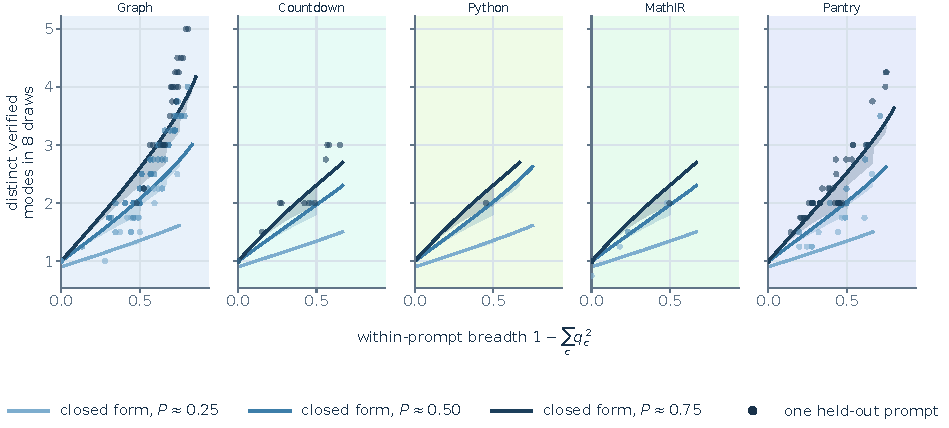
\includegraphics[width=.86\linewidth]{figures/replay_bank_decomposition.pdf}
  \caption{\textbf{Uniform allocation maximizes sampled diversity at fixed buffered probability mass.}
  The horizontal axis traces allocations from a single mode to a uniform
  distribution over $k$ buffered keys. Dashed curves show $1-(1-P)^8$, the
  probability of sampling at least one buffered key when their total mass is
  $P$. Solid curves show the expected number of distinct buffered keys for
  $P\in\{.25,.50,.75\}$; bands span a range of mode counts based on the
  observed prompts and are analytic ranges rather than confidence intervals.
  Points show held-out Level-1 prompts, which have no replay buffer, evaluated
  at the final Re:Dr and
  Re:Max checkpoints of Qwen2.5-0.5B, using one matched seed and grouping
  prompts by their verified response fraction. Their horizontal coordinates
  use empirical key frequencies in $1-\sum_c q_c^2$, rather than the unbiased
  pair estimator. Both coordinates use the same sampled responses, so the
  scatter illustrates agreement with the analytic relationship rather than
  an independent prediction of diversity on new responses.}

  \label{fig:replay-bank-decomposition}
\end{figure}

These properties describe the categorical objective on training-prompt buffers.
Generalization is measured on held-out prompts, whose responses never enter
the buffers. The surrogate alone does not establish that the implemented
response-level objective increases held-out \pmd{}.

% Shared long-paper and workshop benchmark/protocol appendix.

\clearpage
\phantomsection
\begin{center}\large\textbf{Part II. Benchmark and method}\end{center}
\addcontentsline{toc}{part}{Part II. Benchmark and method}

\section{Benchmark and Evaluation Protocol}
\label{app:data}
\label{app:experimental-design}
\label{app:domain-overview}
\label{app:data-inventory}

\mb{} uses a single executable validator to determine correctness and
solution identity, through the map $V(\cdot,s_x)$ defined in
App.~\ref{app:metric-details}. Invalid outputs receive reward zero and no
key; valid outputs receive reward one and a canonical execution key. The
valid-key catalogue and its size are unavailable to the learner and are not
used to schedule replay or determine when training stops.
Table~\ref{tab:tasks} summarizes the five domains and the response variants
that share a key. The datasets are available in the
\href{https://huggingface.co/datasets/od2961/ModeBench}{public release};
the training comparisons in this paper cover Levels 1--3.

\begin{table}[!htbp]
  \centering
  \caption{\textbf{Executable solution identities in the five \mb{} domains.}
  The validator determines both correctness and identity, while the catalogue
  of valid modes is unavailable during training. \emph{Valid modes} reports
  the mean and range of certified catalogue sizes over the Level-1 evaluation
  split. These catalogues need not include every accepted output:
  \texttt{Countdown}, for example, accepts valid keys outside its enumeration.
  \emph{Reached} reports mean distinct verified modes from one hosted
  deployment using 512 draws on 32 prompts
  per domain (Fig.~\ref{fig:gpt56-sampling-budget}). These prompts were
  selected from the evaluation split independently of model outputs. The two
  columns therefore summarize the full split and a subset, respectively.
  \texttt{MathIR}'s catalogue includes longer derivations; limited observed
  coverage does not establish whether these routes are inaccessible or simply
  too rare to observe at the given budget. Higher levels have different
  constructions and mode-count distributions (App.~\ref{app:data-levels}).
  The full prompts and model-specific chat templates appear in App.~\ref{app:prompts}.}

  \label{tab:tasks}
  \scriptsize
  \setlength{\tabcolsep}{5pt}
  \renewcommand{\arraystretch}{1.08}
  \begin{tabularx}{\linewidth}{@{}l
      >{\hsize=1.3\hsize}Y
      >{\hsize=.8\hsize}Y
      >{\hsize=.9\hsize}Y
      rr@{}}
    \toprule
    \textbf{Domain} & \textbf{Generated answer / check} &
    \textbf{Executed key} & \textbf{Equivalent responses} &
    \textbf{Valid modes} & \textbf{Reached} \\
    \midrule
    \texttt{Graph} coloring & Complete assignment; check fixed colors and edges &
    Color vector & Spacing only & 6.27 & 2.53 \\
      & & & & {\scriptsize4--12} & \\
    \addlinespace[2pt]
    \texttt{Countdown} & Parse operands; execute exactly &
    Normalized AST & Commutative order & 4.52 & 3.47 \\
      & & & & {\scriptsize2--8} & \\
    \addlinespace[2pt]
    \texttt{Python} factors & Execute restricted lambda externally &
    Return vector & Programs with the same return vector & 229.44 & 3.75 \\
      & & & & {\scriptsize16--1{,}512} & \\
    \addlinespace[2pt]
    \texttt{MathIR} & Execute bounded action program &
    State trajectory & Programs with the same states & 5.00 & 1.91 \\
      & & & & {\scriptsize5} & \\
    \addlinespace[2pt]
    \texttt{PantryPlan} & Exact ingredient allocation; check all bounds &
    Ingredient support & Quantity and ordering aliases & 18.19 & 6.91 \\
      & & & & {\scriptsize8--40} & \\
    \bottomrule
\end{tabularx}
\end{table}


\subsection{Solution mode definitions and concentration by domain}
\label{app:mode-keying}

\mb{} defines solution modes through three kinds of executable identity.
In \texttt{Countdown} and \texttt{MathIR}, distinct modes are different routes to the same
answer. In \texttt{Python}, they are different return vectors on the public test
inputs. In \texttt{Graph} and \texttt{PantryPlan}, they are different valid answers. The
response budgets also differ (Table~\ref{tab:run-contract}): a \texttt{PantryPlan}
response is a short plan, while a \texttt{Countdown} response is a derivation.
These keys identify verified solutions, not latent reasoning processes.

\paragraph{Sensitivity to the chosen equivalence.}
The canonical key determines which responses count as distinct solutions.
A coarser, task-relevant equivalence can therefore change the measured
diversity gain. App.~\ref{app:coarser-keys} tests one such equivalence per
domain. Most contrasts persist, but the replay gain for Level-3
\texttt{Python} with the original wording falls from $.419$ to zero when
$d$ and $n/d$ are treated as the same unordered factor pair. Among the five
domains, \texttt{Python} is the most sensitive to this choice. Evidence that
the gain extends beyond the original key definitions comes from the other
domains. Training uses the original canonical keys throughout; the coarser
analysis measures sensitivity to alternative definitions of solution identity.

\paragraph{Answer-only training prompts.}
The training prompts request only the final answer
(App.~\ref{app:prompts}), with response budgets chosen accordingly.
Restricting outputs to executable answers allows the validator to determine
solution identity directly, without a learned judge or an embedding-similarity
threshold. The finite solution catalogues also provide the reference values
in Table~\ref{tab:absolute-support-references}. For example, uniform sampling
over the 64 ingredient-selection bit masks in \texttt{PantryPlan} reaches
more verified modes than any trained policy evaluated here.

The training experiments do not measure diversity in long reasoning traces.
The separate hosted-model evaluations include reasoning-enabled deployments
and also exhibit concentration (App.~\ref{app:hosted-mode-diversity}), but
these inference-only observations do not establish how training changes
reasoning behavior.

Across RLVR-only arms, the mean initial-to-terminal increase in conditional
collision is $+0.202$ for route-keyed domains over
98 seed-blocks, $+0.201$ for the behavior-keyed
domain over 15, and $+0.404$ for answer-keyed
domains over 106. All three grouped means increase, with the
largest increase in the answer-keyed group. These comparisons describe
concentration under each definition; differences between domains do not
isolate the effect of choosing a particular key.

\texttt{Countdown}'s mean collision increase is $+0.383$ over
46 seed-blocks, compared with $+0.230$ in \texttt{Graph}.
Thus concentration also occurs among different derivations of a common
answer. \texttt{MathIR} has a smaller increase, $+0.042$. Its certified
catalogue includes longer derivations that are absent from the observed
outputs (App.~\ref{app:algorithm-identity}). Their absence at the evaluated
budgets does not establish that those modes are unreachable.

\paragraph{Explicit-reasoning settings and observed solution counts.}
App.~\ref{app:hosted-reasoning-control} compares five deployments on the
same 480 prompts, with eight responses per prompt and an 8,192-token output
cap in both conditions. Disabling explicit reasoning through the provider
interface lowers overall mean \texttt{distinct@8} in all five deployments:
GPT-5.6 Sol changes from 1.62 to 0.99 and GPT-5.4 from 1.85 to 1.18.
These counts include unsolved prompts and depend on both correctness and
allocation among verified solution modes. Changes in success-conditional
\pmd{} differ across deployments, so lower raw counts do not establish a
common increase in conditional concentration. The requested setting does
not establish the absence of hidden computation, and collection times and
provider defaults can also differ. This comparison therefore describes
solution distributions under the tested configurations, without identifying
an isolated effect of internal deliberation.

\subsection{Dataset splits and validation}
\label{app:data-materialization}

Each domain has disjoint training and evaluation splits
(Table~\ref{tab:run-contract}). \texttt{PantryPlan} and Level 2 also include
separate development splits (App.~\ref{app:data-levels}). For every
\texttt{Python} problem, execution verifies at least two functions with
distinct valid return vectors. For \texttt{MathIR}, each catalogue route is
checked with the same interpreter used to evaluate model outputs.

\begin{table}[!htbp]
\centering
\caption{\textbf{Dataset sizes and certified mode counts.} \texttt{Python} and \texttt{MathIR}
use disjoint training and evaluation splits. Catalogue ranges refer to the
training split; Table~\ref{tab:tasks} gives evaluation-split counts.}

\label{tab:materialization-identities}
\small
\begin{tabular}{@{}lrr@{}}
\toprule
& \textbf{\texttt{Python} factors} & \textbf{\texttt{MathIR} action menu} \\
\midrule
Training problems & 384 & 384 \\
Evaluation problems & 128 & 128 \\
Certified modes per prompt (train) & 16--3{,}600 & 5 \\
\bottomrule
\end{tabular}
\end{table}

\paragraph{\texttt{PantryPlan}.}
\label{app:data-pantry}
\texttt{PantryPlan} contains 384 training, 64 development, and 128 evaluation
prompts across four problem families. The number of feasible ingredient
supports ranges from 8--45 in training and
8--40 in evaluation, with an evaluation mean of
18.19. The validator checks inventory, serving increments, mass,
nutrient bounds, and dietary restrictions using exact arithmetic. The solution
key records which ingredients are used. These checks establish satisfaction
of the stated constraints; they do not assess taste, preparation feasibility,
or food safety.

\subsection{\texttt{Python} execution and validation}
\label{app:python}
\label{app:python-language}

After removing surrounding whitespace, the validator parses each candidate
as a Python expression, with limits of 240 characters and 64 abstract syntax
tree (AST) nodes. The accepted form is \texttt{lambda n: EXPR}, with one
ordinary argument named \texttt{n} and no default value, positional-only,
keyword, or variadic arguments. Integer literals have absolute value at most
10,000. Permitted expressions use \texttt{n}, addition, subtraction,
multiplication, floor division, remainder, integer comparisons, Boolean
\texttt{and}/\texttt{or}, unary plus/minus/\texttt{not}, and conditionals.
The validator rejects Boolean and non-integer literals, calls, imports,
attributes, comprehensions, containers, subscripts, assignment, loops, and
other identifiers.

The task specification contains $J$ distinct integers in $[4,1000]$, with
$2\le J\le8$. Every Level-1 problem uses 4 inputs drawn from
$[6,96]$ and admits at least two valid return vectors.

\paragraph{External execution.}
\label{app:python-process}
Candidate expressions run in an isolated Python process with an empty
\texttt{\_\_builtins\_\_} environment. The process repeats the syntax checks
and evaluates the function on the fixed inputs, subject to a 0.25-second
execution limit and a one-second response deadline. Timeouts, execution errors,
malformed results, non-integer outputs, and failed divisor checks produce
$\bot$ and zero reward. Only a validated integer return vector receives a key.

\paragraph{Behavioral identity.}
\label{app:python-identity}
For each of the $J$ fixed inputs $n_j$, the returned $d_j$ must be an integer
but not a Boolean, satisfy $1<d_j<n_j$, and divide $n_j$ exactly. All checks
must pass. The key is the ordered return vector $(d_1,\ldots,d_J)$;
two programs share a key exactly when these vectors agree. The exact support count
$\prod_j|\{d:1<d<n_j,\ d\mid n_j\}|$ is used only for dataset validation.

\subsection{Matched level constructions}
\label{app:data-levels}

Levels 2--5 expand the search space while preserving the verifier,
canonicalizer, and solution-mode definition. Level 2 is harder for the same
model; Levels 3--5 are calibrated against a fixed Level-1 reference using
larger models, with an exception for Level-4 \texttt{MathIR}.

\paragraph{Level 2.}
Level 2 contains 384 training, 128 development, and 128 evaluation problems,
with no shared problem identities across its splits or with Level 1.
The training distribution of valid-key counts matches that of Level 1.
For \texttt{Graph}, \texttt{Countdown}, \texttt{Python}, and \texttt{MathIR},
the development and evaluation distributions match separate Level-1 reference
sets used for dataset construction. \texttt{PantryPlan} uses its existing
Level-1 splits as references; its 64-prompt development histogram is scaled
by two to define the target counts for the 128-prompt Level-2 development set.

The Level-1 construction reference sets differ from the evaluation sets used
to compare trained policies. Consequently, those evaluation sets have different
valid-key-count distributions across levels in \texttt{Graph},
\texttt{Countdown}, and \texttt{Python}. Cross-level differences reflect both
problem structure and evaluation population, and cannot isolate difficulty
at a fixed distribution of mode counts. Within each level, replay and control
conditions use the same prompts, seeds, fresh-sample objective, and training
budget.

\begin{table}[!htbp]
\centering
\caption{\textbf{Structural differences between Levels 1 and 2.}
The verifier, canonicalizer, and definition of a solution mode are unchanged;
Level 2 expands the search space.}
\label{tab:level2-structure}
\small
\begin{tabularx}{.96\linewidth}{@{}lYY@{}}
\toprule
\textbf{Domain} & \textbf{Level 1} & \textbf{Level 2 structural change} \\
\midrule
\texttt{Graph} coloring & Three hidden vertices & Four hidden vertices \\
\texttt{Countdown} & Three operands & Four operands, with values up to 14 \\
\texttt{Python} factors & Four executed cases, all at most 96 & Four cases, including a value above 96 \\
\texttt{MathIR} & One-sided linear families & Variable-on-both-sides families \\
\texttt{PantryPlan} & Base dietary/composition constraints & More active dietary exclusions and tighter composition \\
\bottomrule
\end{tabularx}
\end{table}

On every domain's development split, fixed Qwen2.5-0.5B has
\texttt{pass@8} in $[.10,.90]$, below its Level-1 construction reference
when both levels use identical decoding settings.

\paragraph{Scale-calibrated Level 3.}
Level 3 is calibrated using Qwen2.5-3B, with Qwen2.5-0.5B on Level 1 as the
reference. Model weights remain fixed. Construction parameters are fitted
on development problems and assessed on held-out prompts. In every domain,
the calibration requires absolute differences from the reference of at most
$.04$ in pass@1 and $.08$ in pass@8, measured using four independent groups
of eight samples per prompt. \distk{} is excluded from the fitting objective.

Both models use their native chat templates, temperature 1, top-$p$ 1, and a
192-token generation limit. \texttt{Graph} prompts request only a boxed final
answer. The other domains receive task-specific solution guidance and use
decoding constrained to legal output syntax, without filtering candidates by
correctness. These criteria establish an empirical match to the reference
success rates rather than a formal two-sided equivalence test.
The Level-3 \texttt{Python} hint ablation removes the strategy guidance
(App.~\ref{app:prompt-hint-ablation}); its difficulty is therefore outside
the scope of this calibration.

\paragraph{Levels 4 and 5.}
Levels 4 and 5 are calibrated with 7B and 14B models, respectively, against
the same Qwen2.5-0.5B Level-1 reference, using pass@1 and pass@8 tolerances
of $.04$ and $.08$.
Level 5 meets these criteria in all five domains. Level 4 meets them in \texttt{Graph},
\texttt{Countdown}, \texttt{Python}, and \texttt{PantryPlan}, but not \texttt{MathIR}.

For \texttt{MathIR}, the reference pass@8/pass@1 ratio is $5.50$, whereas
the largest ratio among the evaluated 7B constructions is $4.16$. A ratio
of mixture means cannot exceed the largest component ratio, so mixing these
constructions cannot reproduce the reference ratio exactly.

The heterogeneity gap, $1-(1-\bar P)^8-\overline{\texttt{pass@8}}$, compares
observed pass@8 with its value if every prompt had the same correctness
$\bar P$. The measured gaps are $.169$--$.398$ at 7B and $.060$ for the
reference. Because the gap depends on mean correctness $\bar P$, these values
are not directly comparable across correctness levels. Each Level-4 domain
contains 384 training, 128 development, and 128 evaluation prompts, disjoint
from other levels. Level-4 \texttt{MathIR} appears in
Figs.~\ref{fig:base-levels-all-scales} and~\ref{fig:level-construction}
but is not difficulty-matched to the reference.

\subsection{Model performance across all five levels}
\label{app:base-levels-all-scales}

Fig.~\ref{fig:base-levels-all-scales} compares Qwen2.5-Instruct across five
levels and domains; Fig.~\ref{fig:families-appendix} adds three model families,
for 375 model--domain--level measurements before benchmark training.
Each measurement uses the same 128 held-out prompts per domain and level,
with four independent groups of eight responses per prompt, totaling 4,096
responses. For \texttt{pass@8} and \distk{}, we score each group, average
within prompts, and then average prompts. For \pmd{}, we pool the four
groups within each prompt (App.~\ref{app:metric-sampling}).

Evaluation uses native chat templates, temperature 1, top-$p=1$, and a
192-token output limit. \texttt{Graph} prompts request boxed final answers;
other domains use task-specific solution guidance and syntax-constrained
decoding. These settings differ from the training evaluations: under the
training template and its larger sample, the same untrained Level-1
\texttt{Python} model defines \pmd{} on 73 of 128 prompts, with mean $.168$
(Section~\ref{sec:results-collapse}). Training effects are therefore measured
against the untrained model under the corresponding evaluation conditions.

Success does not necessarily decrease monotonically with level.
\texttt{pass@8} at the highest evaluated level is below its Level-1 value in
33 of 35 model--domain series. Model scale and
benchmark level also affect diversity differently: the median range of
\pmd{} across scales at a fixed level is .251, compared with
.104 across levels at a fixed scale.

\begin{figure}[!htbp]
  \centering
  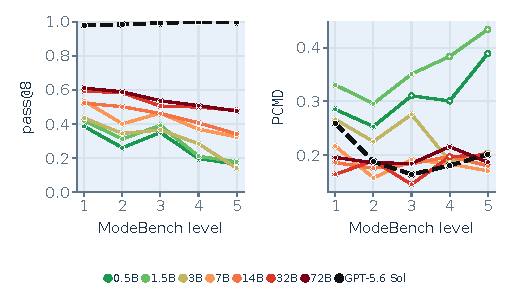
\includegraphics[width=.62\linewidth]{figures/qwen_level_trends.pdf}
  \caption{\textbf{Accuracy and solution diversity vary differently across benchmark levels.}
  Left: \texttt{pass@8}; right: \pmd{}, averaged with equal domain weights
  for each Qwen2.5-Instruct scale (colored lines) and GPT-5.6 Sol (black dashed
  line). This Qwen evaluation augments the 128 held-out prompts with the 384
  training-split prompts where available; none were used to train these
  checkpoints. Filled diversity markers indicate at least 30 prompts with
  two or more correct responses in every domain. Hollow markers average the
  available estimates when at least one domain has insufficient support;
  the set of contributing domains can differ when an estimate is undefined.}

  \label{fig:qwen-level-trends}
\end{figure}

\begin{figure}[!htbp]
  \centering
  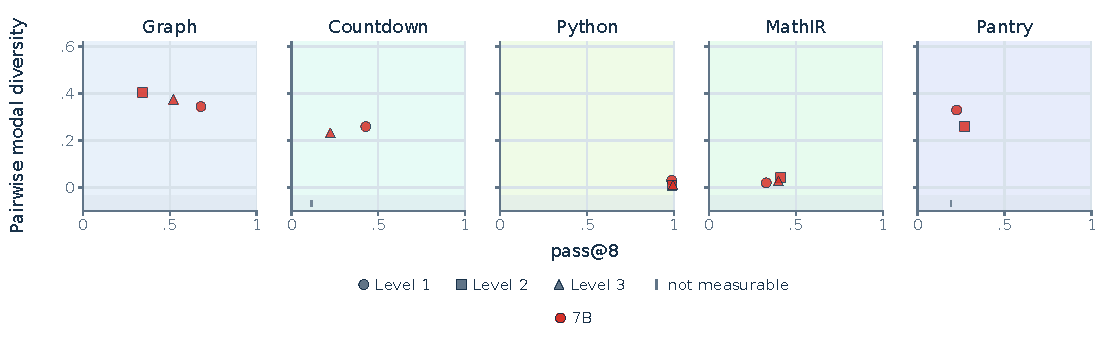
\includegraphics[width=\linewidth]{figures/mode_diversity_level_construction.pdf}
  \caption{\textbf{High accuracy can coexist with low solution diversity.}
  Each row shows one checkpoint before benchmark training, with domains in
  columns, \texttt{pass@8} on the horizontal axis, and \pmd{} on the vertical
  axis. Color indicates parameter count and marker shape indicates level.
  Each measurement uses four groups of eight responses to 128 held-out
  prompts at temperature 1; \pmd{} pools the groups within each prompt.
  Filled markers indicate at least 30 prompts with two or more correct
  responses. Hollow markers indicate 5--29 such prompts and show one standard
  error. Ticks below the axis mark measurements with fewer than five eligible prompts.}

  \label{fig:level-construction}
\end{figure}

\begin{figure}[!htbp]
  \centering
  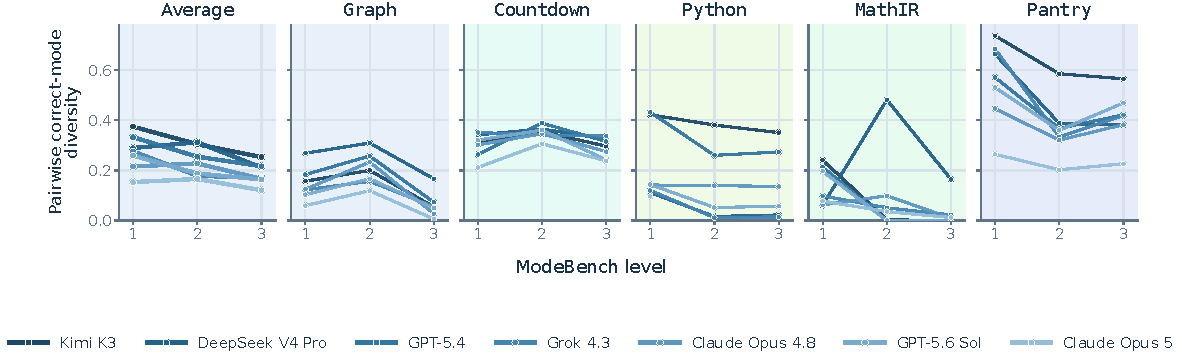
\includegraphics[width=\linewidth]{figures/frontier_level_grid.pdf}
  \caption{\textbf{Mean solution diversity is lower at Level 3 than at Level 1 for every evaluated hosted deployment.}
  Lines show \pmd{} for 7 deployments, with eight
  responses to each of 128 held-out prompts per domain and level. Panels show
  individual domains and their equally weighted mean. For each deployment,
  the set of domains contributing to the mean is fixed across levels.
  Darker lines indicate higher overall diversity. Hollow markers fall below
  the 30-prompt support threshold and are excluded from connecting lines.
  Higher levels change problem structure and add strategy guidance in
  \texttt{MathIR}, \texttt{Python}, and \texttt{PantryPlan}
  (App.~\ref{app:prompt-hint-ablation}); these curves reflect both changes.}

  \label{fig:frontier-level-grid}
\end{figure}

\begin{figure}[!htbp]
  \centering
  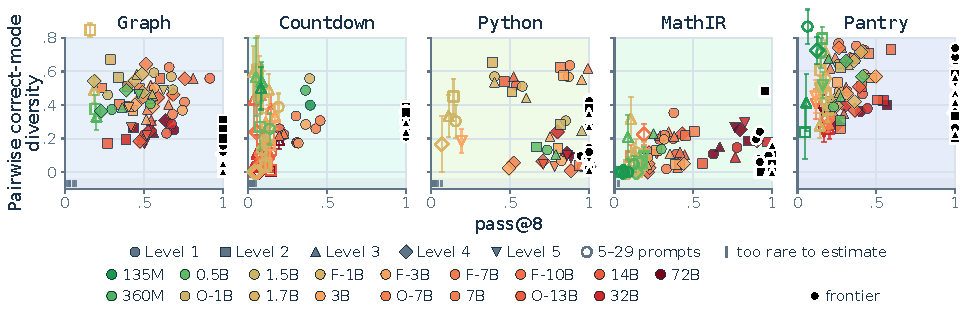
\includegraphics[width=.92\linewidth]{figures/mode_diversity_families_appendix.pdf}
  \caption{\textbf{Models of similar size can differ in solution diversity.}
  SmolLM2, Qwen2.5, Falcon3, and OLMo-2 checkpoints are compared by
  \texttt{pass@8} and \pmd{} across five domains and the available levels,
  before benchmark training. Color indicates parameter count on a logarithmic
  scale; marker shape indicates level. Black markers show the
  7 hosted deployments. Local models use four groups
  of eight responses to 128 held-out prompts per domain and level; hosted
  deployments use eight responses per prompt. Filled markers indicate at
  least 30 prompts with two or more correct responses. Hollow markers
  indicate 5--29 and show one standard error. Ticks below the axis indicate
  fewer than five eligible prompts, for which no diversity estimate is reported.}

  \label{fig:families-appendix}
\end{figure}


\FloatBarrier
\subsection{Other model families at matched scale}
\label{sec:families-appendix}

Fig.~\ref{fig:families-appendix} compares SmolLM2, Qwen2.5, Falcon3, and
OLMo-2 on the same 128 held-out prompts per domain and level. All use four
groups of eight responses, the same verifier, and the same eligibility
thresholds. Comparisons across families use the 4 shared
levels; only Qwen2.5 is evaluated at Level 5. Color denotes parameter count.

Families differ in diversity even at similar parameter counts. Near 7B,
Qwen2.5, Falcon3, and OLMo-2 have different \pmd{} values despite similar
\texttt{pass@8}. Their ordering persists in the 10--15B range, where Falcon3
and OLMo-2 are close. Within parameter-count bands, the median range of
\pmd{} across family means is .166, compared with
.198 across scales within a family, over the
4 shared levels. The earlier .251 summary instead
compares all seven Qwen scales at each level. These descriptive comparisons
do not isolate which pretraining or post-training choices account for the
differences between models.

\clearpage
\subsection{Training and evaluation settings}
\label{app:repro-run-contract}
\label{app:comparison-design}

% [H] pinned this table to the head of the subsection, and being too tall for
% what the previous page had left it took a page of its own and stranded the
% remainder. Floating lets the prose that follows it close the gap.
\begin{table}[!htbp]
  \centering
  \caption{\textbf{Paired comparisons use the same numbers of optimizer updates and fresh rollouts.}
  Treatment and control share the settings below. Both compute replay scores
  and execute the backward pass, but the replay gradient is exactly zero in
  the control. Their buffer contents can differ, so replay workloads, total
  floating-point operations, and wall-clock time are not matched. The control
  receives no additional training in place of replay computation
  (App.~\ref{app:compute-matching}).}

  \label{tab:run-contract}
  \small
  \begin{tabularx}{\linewidth}{@{}P{.23\linewidth}Y@{}}
    \toprule
    \textbf{Component} & \textbf{Setting} \\
    \midrule
    Data & 384 training and 128 disjoint evaluation prompts per domain and
      level; evaluation prompts are excluded from training and replay. \\
    Fresh rollouts & $G=16$, temperature 1, top-$p=1$; one prompt group per update. \\
    Optimization & Eight training passes (3,072 updates), with one PPO epoch
      per batch. $\beta_{\mathrm{KL}}=0$ except in the reference-KL comparison
      (App.~\ref{app:kl-measured}), which varies only this coefficient.
      Paired conditions share initialization, prompt order, optimizer,
      hardware class, and checkpoint frequency. \\
    Evaluation & At passes $0,.5,\ldots,8$: four groups of eight responses
      per prompt at temperature 1 and top-$p=1$, plus a separate greedy
      response at temperature 0. Final comparisons use the last checkpoint. \\
    Replay & Capacity $M=16$ keys per prompt; buffers are selected in
      round-robin order, one per update; $\lambda_{\mathrm{replay}}=.10$.
      The control has zero replay gradient; buffer contents and computational
      workloads may differ between conditions. \\
    Training seeds & Five per model--domain combination; paired comparisons use
      common seeds, with sample sizes reported alongside the results. \\
    Learning rate & Qwen2.5-0.5B and Falcon3-1B: constant $2\times10^{-7}$,
      with Falcon optimizer states stored on the CPU. Qwen2.5-3B: cosine
      decay from a $10^{-7}$ peak to a $10^{-8}$ floor, with 10\% warmup. \\
    Optimizer & Fused Adam in \texttt{bf16} with decoupled weight decay,
      $\beta_1=.9$, $\beta_2=.95$, weight decay $0$, gradient-norm clip $1.0$,
      with gradient checkpointing. CPU offloading uses the corresponding
      CPU optimizer implementation with the same hyperparameters. \\
    Policy update & Parameters are synchronized after every update, and each
      rollout is used once in a single PPO epoch. The symmetric clipping
      threshold is $\varepsilon=.2$. The importance ratio equals $1$ when
      the surrogate is evaluated in this update scheme, so clipping is inactive. \\
    % All twelve cells are the OAT_ZERO_GENERATE_MAX_LENGTH actually submitted,
    % read per domain from the job ledgers rather than from a launcher default:
    %   0.5B  var/artifacts/e72_frontier_source_runs.json
    %           (inherited_eval_config.generate_max_length; the 3B cohort
    %            inherits this record and overrides only the base model)
    %   1B    var/artifacts/e79_falcon1b_aligned_verified_replay_jobs.json
    %   3B    var/artifacts/e80r1_qwen3b_aligned_verified_replay_jobs.json
    % ops/train.sh defaults this to 192, so a domain that is 192 looks the same
    % whether it was chosen or inherited; the ledgers are what distinguish them.
    Response tokens & \texttt{Graph} and \texttt{Countdown}: 192; \texttt{Python}: 192/512/192
      at 0.5B/1B/3B; \texttt{MathIR}: 64/128/64; \texttt{PantryPlan}: 8. \\
    \bottomrule
  \end{tabularx}
\end{table}



For each training seed, \texttt{pass@8} and \texttt{distinct@8} are averaged
over four eight-response groups per prompt and all 128 evaluation prompts;
\texttt{mean@8} is the fraction of correct responses. Responses are independent
within a group. Independence across groups, required for the pooled \pmd{}
interpretation, depends on the sampling procedure described in
App.~\ref{app:metric-sampling}. Evaluation outputs are excluded from training
and replay, and do not determine checkpoint selection or stopping.

Comparisons use paired final checkpoints. Comparisons with five matched
training seeds use nominal pointwise 95\% Student-$t$ intervals; other main
checkpoint comparisons report sample sizes and descriptive means. Diversity
comparisons use the prompt-eligibility thresholds and interval procedures
specified alongside their results. Intervals condition on the fixed evaluation
prompts and sampled responses. The replay-weighting comparison instead uses
a bootstrap over paired training seeds.

% Finish benchmark floats before beginning the prompt examples.
\FloatBarrier
\section{Exact Domain Prompts}
\label{app:prompts}

Each domain's training prompt contains one system message and one user
message, without few-shot examples. Training and evaluation use the same
template within each method. The examples below reproduce the first prompt
from each Level-1 evaluation split in Qwen's chat format. Falcon3 uses the
same message text with its own \texttt{<|system|>} and \texttt{<|user|>}
markers. Models evaluated before benchmark training use their tokenizer's
native chat template (App.~\ref{app:base-levels-all-scales}).
App.~\ref{app:data-levels} describes the different problems and prompting
conditions at Levels 2--5.

The examples preserve the prompt text. A continuation line indented by two
spaces indicates a display line break; replacing that break and indentation
with one space recovers the original text. In the \texttt{PantryPlan}
example, a line break without this indentation is part of the prompt.

% BEGIN generated by ops/check_paper_domain_prompts.py

\filbreak
\subsection{\texttt{Graph} coloring}
\label{app:prompt-graph}

\noindent 384 training and 128 evaluation prompts.

\begin{Verbatim}[fontsize=\scriptsize,frame=single,framesep=4pt,rulecolor=\color{black!25},samepage=true]
<|im_start|>system
Return only the final answer inside \boxed{}. Do not explain.<|im_end|>
<|im_start|>user
Color this graph with vertices 1 through 6. The undirected edges are: (1,2), (1,3),
  (3,5), (3,6), (4,6), (5,6). Assign each vertex one color from {1, 2, 3} so that no
  edge has the same color on both endpoints. A partial coloring is 2??1?2, where ?
  means uncolored. Keep every shown digit fixed. There are exactly 3 question marks.
  Return exactly one final answer and no explanation: exactly 3 digits, each one 1,
  2, or 3, for the missing positions from left to right, inside \boxed{}.<|im_end|>
<|im_start|>assistant
\end{Verbatim}

\filbreak
\subsection{\texttt{Countdown}}
\label{app:prompt-countdown}

\noindent 384 training and 128 evaluation prompts.

\begin{Verbatim}[fontsize=\scriptsize,frame=single,framesep=4pt,rulecolor=\color{black!25},samepage=true]
<|im_start|>system
Return only the final answer inside \boxed{}. Do not explain.<|im_end|>
<|im_start|>user
Using the numbers [3, 6, 9], create an arithmetic expression that equals 18. Use
  each given number exactly once. You may use +, -, *, /, and parentheses. Return
  exactly one final answer and no explanation: the expression inside
  \boxed{}.<|im_end|>
<|im_start|>assistant
\end{Verbatim}

\filbreak
\subsection{\texttt{Python} factors}
\label{app:prompt-python}

\noindent 384 training and 128 evaluation prompts.

\begin{Verbatim}[fontsize=\scriptsize,frame=single,framesep=4pt,rulecolor=\color{black!25},samepage=true]
<|im_start|>system
Return only the final answer inside \boxed{}. Do not explain.<|im_end|>
<|im_start|>user
Write one pure Python function with the exact form lambda n: EXPR. An external
  Python tool will call it once for each n in [18, 82, 91, 93]. For every call,
  return an integer d satisfying 1 < d < n and n % d == 0. Different valid return
  vectors are different solution modes. You may use integer literals, n, +, -, *,
  //, %, comparisons, Boolean operators, and conditional expressions; calls,
  imports, attributes, containers, and other names are forbidden. Return exactly the
  one-line lambda inside \boxed{} and no explanation.<|im_end|>
<|im_start|>assistant
\end{Verbatim}

\filbreak
\subsection{\texttt{MathIR} action menu}
\label{app:prompt-mathir}

\noindent 384 training and 128 evaluation prompts.

\begin{Verbatim}[fontsize=\scriptsize,frame=single,framesep=4pt,rulecolor=\color{black!25},samepage=true]
<|im_start|>system
Return only the final answer inside \boxed{}. Do not explain.<|im_end|>
<|im_start|>user
MathIR linear-menu-v1. Solve for x by choosing an executable action sequence. Every
  selected action is applied exactly to BOTH sides of the current equation, followed
  by exact simplification. Bindings: a=2, b=-9, c=-1. Initial equation: x/a + b = c.
  Action menu: A means div(a); B means add(b); C means sub(b); D means sub(c); E
  means sub(mul(a,b)); F means mul(a). Choose 1-4 action IDs. Illegal operations,
  repeated states, and paths that do not finish with x isolated are rejected. Return
  only the IDs separated by semicolons inside the answer box; for example formatting
  only: \boxed{A;C}. Do not return x's numeric value.<|im_end|>
<|im_start|>assistant
\end{Verbatim}

\subsection{\texttt{PantryPlan}}
\label{app:prompt-pantry}

\noindent 384 training and 128 evaluation prompts.

\begin{Verbatim}[fontsize=\scriptsize,frame=single,framesep=4pt,rulecolor=\color{black!25},samepage=false]
<|im_start|>system
Return only six binary digits and no other text. Each digit maps to the
  corresponding Pantry row in printed order. A trusted environment will choose exact
  quantities on precisely the selected rows.<|im_end|>
<|im_start|>user
Create one feasible high fiber snack from this frozen pantry.
Nutrition values are per 100 g. Quantities are exact integer grams.

Pantry:
- almonds: available=100g, step=25g, minimum-if-used=50g; energy=584kcal,
  protein=21.5g, fiber=10.8g, sodium=0.0mg; tags=tree_nut
- banana: available=125g, step=25g, minimum-if-used=50g; energy=97.0kcal,
  protein=0.74g, fiber=4.62g, sodium=0.0mg; tags=none
- carrots: available=150g, step=25g, minimum-if-used=50g; energy=45.0kcal,
  protein=0.941g, fiber=3.1g, sodium=86.6mg; tags=none
- grape_tomatoes: available=100g, step=25g, minimum-if-used=50g; energy=27.0kcal,
  protein=0.83g, fiber=2.1g, sodium=6.0mg; tags=none
- navel_orange: available=150g, step=25g, minimum-if-used=50g; energy=47.0kcal,
  protein=0.91g, fiber=2.0g, sodium=9.0mg; tags=none
- sunflower_seeds: available=125g, step=25g, minimum-if-used=50g; energy=571kcal,
  protein=18.9g, fiber=7.22g, sodium=0.0mg; tags=none

Use 2 to 4 ingredients.
Forbidden tags: none
Targets:
- mass_g: minimum 125, maximum 200
- energy_kcal: minimum 239.4, maximum 432.25
- protein_g: minimum 6.423
- fiber_g: minimum 3.478
- sodium_mg: maximum 37.6

Choose the ingredient support as a six-bit mask in the exact Pantry row order. Bit 1
  includes that row and bit 0 excludes it.<|im_end|>
<|im_start|>assistant
\end{Verbatim}

% END generated by ops/check_paper_domain_prompts.py

% Shared exact replay update; empirical comparisons are in results.tex.

\section{Replay Algorithm}
\label{app:algorithm}

Verified replay combines learning from newly sampled responses with a
likelihood loss on stored, verified solutions. Each prompt $x$ has a buffer
$\mathcal B_x$ of at most $M$ exemplars, with one response per canonical key.
A round-robin cursor $\sigma$ selects one prompt's buffer at each update,
and all keys in that buffer contribute equally to the replay loss.
Table~\ref{tab:notation} defines the notation;
App.~\ref{app:replay-metric-alignment} relates this objective to diversity.

\subsection{Fresh task advantages}
\label{app:binary-maxrl}

For a group of $G$ fresh responses with verified binary rewards $R_i$ and
$R=\sum_i R_i$, Dr.GRPO uses $A_i=R_i-R/G$, while MaxRL uses
\[
 A_i^{\mathrm{MaxRL}}=
 \begin{cases}
 G R_i/R-1, & R>0,\\
 0, & R=0.
 \end{cases}
\]
The centered MaxRL estimator \citep{tajwar2026maxrl} assigns advantage $-1$
to failures in mixed groups and gives each success greater weight when
successes are scarce. Both objectives assign zero task advantage to every
response in an all-correct or all-failure group. Lemma~\ref{lem:maxrl-mean}
derives MaxRL's mean objective as a harmonic combination of pass@\(k\)
terms. These advantages apply to fresh responses; stored exemplars contribute
through the separate replay loss.

\subsection{Optimizer update}
\label{app:algorithm-update}

\begin{algorithm}[H]
  \caption{\textbf{Verified replay update.} The fresh objective selects Re:Dr or Re:Max.}
  \label{alg:verified-replay-update}
  \small
  \begin{algorithmic}[1]
    \REQUIRE Policy $\pi_\theta$; prompt $x$ and verifier specification
      $s_x$; group size $G$; fresh objective
      $o\in\{\mathrm{MaxRL},\mathrm{Dr.GRPO}\}$; replay weight
      $\lambda_{\mathrm{replay}}$; buffer capacity $M$; buffers and cursor
      $(\mathcal B,\sigma)$
    \ENSURE Updated $(\theta',\mathcal B',\sigma')$
    \STATE Draw the on-policy group
      $\mathcal G=\{y_i\sim\pi_\theta(\cdot\mid x)\}_{i=1}^G$
    \FOR{$i=1,\ldots,G$}
      \STATE Execute $\widetilde c_i\gets V(y_i,s_x)$ and observe task
        reward $R_i$
      \STATE Set $c_i\gets\widetilde c_i$ iff
        $R_i>0\wedge\widetilde c_i\ne\bot$; otherwise set $c_i\gets\bot$
    \ENDFOR
    \STATE Compute fresh task advantages $A_i^{o}$ from $\{R_j\}_{j=1}^G$;
      for $o=\mathrm{MaxRL}$ use the formula in App.~\ref{app:binary-maxrl}
    \STATE After the full group is validated, deterministically retain one
      policy exemplar for each new $c_i\ne\bot$ in $\mathcal B_x$, up to
      capacity $M$
    \STATE $(z,\sigma')\gets\textsc{NextBuffer}
      (\{\mathcal B_u\}_u,\sigma)$ by a fixed round-robin cursor over
      prompts; the replayed prompt $z$ need not be the prompt $x$ that
      supplied the fresh group
    \IF{a replay buffer $\mathcal B_z$ exists}
      \STATE For each exemplar $e_c\in\mathcal B_z$, compute
        $\ell_c=|e_c|^{-1}\log\pi_\theta(e_c\mid z)$
      \STATE $L_{\mathrm{replay}}\gets-|\mathcal B_z|^{-1}
        \sum_{c\in\mathcal B_z}\ell_c$
    \ELSE
      \STATE $L_{\mathrm{replay}}\gets0$
    \ENDIF
    \STATE Set the replay-loss normalization $w_{\mathrm{rep}}\gets(G-1)/G^2$
    \STATE $\theta'\gets\textsc{Update}
      (\theta,L_{\mathrm{PPO}}(A^{o})
      +w_{\mathrm{rep}}\lambda_{\mathrm{replay}}L_{\mathrm{replay}})$
\end{algorithmic}
\end{algorithm}

\subsection{Buffer construction and scheduling}
\label{app:algorithm-bank}

Each buffer is associated with an exact prompt-token sequence. A response
is eligible for storage if it has positive task reward and a valid canonical
key, including responses that reach the generation limit. The entire group
is validated before the buffer is updated. For each newly observed key, we
retain the lexicographically smallest normalized response-token sequence;
new keys are inserted in sorted order. Selection therefore does not depend
on the order of responses within the group. Each buffer holds at most
$M=16$ exemplars, one per key, with no eviction or replacement. Keys first
observed after the buffer is full receive no replay support.

At each update, a deterministic round-robin schedule selects one nonempty
buffer, including buffers containing a single exemplar. The choice does not
use reward magnitudes, evaluation results, a target mode count, or entropy.
The policy scores every stored response in the selected buffer by teacher
forcing, conditioned on its original prompt. Each exemplar contributes its
mean response-token log probability, excluding prompt and padding tokens.

The replay loss is the negative mean score over the selected keys,
weighted by $\lambda_{\mathrm{replay}}(G-1)/G^2$
(Algorithm~\ref{alg:verified-replay-update}). The normalization $(G-1)/G^2$
matches the weight of a single success in a centered Dr.GRPO group: its
advantage is $(G-1)/G$, followed by averaging over $G$ responses
(Lemma~\ref{lem:grpo-mean}). This loss uses only discovered training
exemplars; it requires neither the complete valid-key catalogue nor
evaluation outputs.

\subsection{Control without replay gradients}
\label{app:algorithm-control}

Replay and control use the same validation, buffer construction, scheduling,
and exemplar-scoring procedures. The control sets the replay gradient to
zero while retaining the forward and backward computations. Both conditions
combine the fresh-task and replay gradients in one optimizer step; the
replay gradient is their only difference in the learning objective.

As the policies diverge, they can generate different responses and accumulate
different buffers, which changes the selected exemplars and their lengths.
The conditions match optimizer updates and fresh-rollout budgets, but not
realized floating-point operations or wall-clock time. The control receives
no additional task-gradient updates, fresh rollouts, or training time in
place of replay computation. The comparison isolates the contribution of the
replay learning signal under this design, without establishing an advantage
at equal total compute (App.~\ref{app:compute-matching}).

\subsection{Verifier requirements and applicability}
\label{app:algorithm-identity}

Replay requires a deterministic rule for grouping verified responses into
solution modes. Its canonical key must be computable for every training
response at reasonable cost and must reflect the task's definition of a
solution. In \mb{}, one executable validator determines both correctness
and identity, so buffer construction requires no learned judge or
embedding-similarity threshold.

Final-answer grading, as used for MATH, GSM8K, and AIME, does not distinguish
derivations of the same answer. When a prompt has only one correct answer,
an answer-based key places every successful response in the same mode. The
buffer then holds one exemplar, and replay reinforces it without balancing
alternative derivations. That buffer is the capacity-one arm of
App.~\ref{app:mode-agnostic-replay}, which retains 58\% of the
Re:Dr diversity effect and a correctness gain of +.263 against
Re:Dr's +.352. Measuring and replaying distinct derivations
requires a finer definition of identity.

\texttt{MathIR} uses executed state trajectories as keys. Its catalogue
includes verified four-state routes, but none appears among 27,450
verified draws. Across 115 solved Level-1 prompts, these
draws cover 67\% of the certified two-state modes and
52\% of the three-state modes. Different modes rarely appear
for the same prompt. Terminal \pmd{} averages .006, corresponding
to 1.01 effective verified modes per prompt. These results provide
limited evidence for diversity gains among alternative derivations.

Across the 6 comparisons, including \texttt{MathIR} in the
five-domain mean reduces the \pmd{} gain by .010--.074
relative to the corresponding four-domain mean. At Qwen2.5-0.5B, the Re:Dr
gain is +.294 across all five domains and +.364 across the other
four. App.~\ref{app:hosted-mode-diversity} reports hosted-model results for
the same four-domain subset.

For open-ended derivations, a learned judge could supply a novelty criterion,
but that criterion would require independent validation. Judge decisions can
be inconsistent or disagree with task correctness, and replay may reinforce
distinctions that the judge rewards without improving solution diversity.
Fixing the judge model, prompt, and decoding rule does not by itself ensure
a valid equivalence relation. Where executable keys are available, they can
be used to assess the judge and measure diversity separately from its training
signal. We do not evaluate judge-based replay here.

\subsection{Exemplar quality and length}
\label{app:algorithm-quality}

Canonical verification establishes that a response satisfies the task
constraints. It does not validate every intermediate reasoning step: a
verified response may be verbose or include an unsound explanation. Replay
weights exemplars by solution key without ranking their reasoning quality.

Each key occupies one buffer entry and contributes its exemplar's mean
response-token log probability,
$\ell_c=|e_c|^{-1}\log\pi_\theta(e_c\mid z)$. Longer responses therefore do
not receive more buffer entries or loss weight proportional to their token
count. This normalization still affects the learning target. In a categorical
surrogate with one exemplar of fixed length $L_b$ per key, the effective
weights are proportional to $L_b^{-1}$. With full coverage, the limiting
distribution favors shorter exemplars and is uniform only when lengths are
equal (App.~\ref{app:theory-replay}). This conclusion concerns the surrogate;
mean-token normalization does not imply uniform key probabilities in a
language model or guarantee concise, sound explanations.

Additional length or reasoning-quality filters would change which exemplars
enter or remain in the buffer, and hence change the replay target. We use no
such filters beyond the stated generation limits and verification rules.
Restricting length can exclude valid alternatives: \texttt{MathIR} includes
longer state trajectories, and the observed lambdas for rarer \texttt{Python}
return vectors are longer than those for the modal vector. Evaluating a
quality filter would therefore require measuring both solution quality and
diversity among retained modes.

\section{Fixed Semantic-MaxEnt Comparator}
\label{app:semantic-maxent}

Fixed Semantic-MaxEnt adds a frequency-based bonus to the fresh-response
advantage. It counts previously observed verified keys but does not optimize
the likelihood of stored exemplars. For response $i$ in a group of $G$
responses to prompt $x$, let $n_x(a)$ count earlier successful responses
with key $a$, and let $m_{-i}(a)$ count successful responses with that key
among the other members of the current group. Write
$N_x=\sum_a n_x(a)$, $S_{-i}=\sum_a m_{-i}(a)\le G-1$, and let
$\mathcal K_i$ contain all keys observed in these two sources. Adding one
pseudocount per observed key and reserving one for unseen keys gives,
for $a\in\mathcal K_i$,

\begin{equation}
  \hat p_i(a)=\frac{n_x(a)+m_{-i}(a)+1}{N_x+S_{-i}+|\mathcal K_i|+1},\qquad
  \hat p_i(\textsc{unseen})=\frac{1}{N_x+S_{-i}+|\mathcal K_i|+1}.
  \label{eq:open-set-predictor}
\end{equation}
A response whose key is outside $\mathcal K_i$ receives the probability
assigned to the unseen category. Invalid and unsuccessful responses do not
contribute to the counts.

\paragraph{Counts and advantage calculation.}
Counts are specific to each exact prompt-token sequence and accumulate
throughout training without decay or reset. Only responses with positive
reward and a valid key are counted. Each response is scored using previous
groups and the other successful responses in its current group. Counts for
the full current group are added only after scoring, so a response never
contributes to its own predicted probability.
The added advantage for an eligible successful response is held constant
during differentiation and equals

\begin{equation}
  A^{\rm sem}_{i,t}=\eta\,
  \frac{\min\{-\log\hat p_i(a_i),\kappa\}
    -\E_{\hat p_i}[\min\{-\log\hat p_i(a),\kappa\}]}{\kappa},
  \qquad \eta=.10,\ \kappa=5.
  \label{eq:legacy-semantic-advantage}
\end{equation}
The same $A^{\rm sem}_{i,t}$ applies at every token position $t$ of response
$i$. Invalid and unsuccessful responses receive zero bonus. The fixed scale
$\eta$ bounds the centered bonus in magnitude, while $\kappa$ clips the
surprisal. The bonus can favor an underrepresented verified mode when that
mode appears in a fresh response, but it adds no direct likelihood term for
a stored exemplar absent from the group. If neither previous groups nor the other
successful responses provide a key, the unseen category has probability one
and the bonus is zero. App.~\ref{app:ucpo-progress} reports the comparison.

\paragraph{Relation to conditional entropy.}

For the true conditional distribution $q_\theta=p_\theta(\cdot\mid\mathcal C)$,
\begin{equation}
 \nabla_\theta H(q_\theta)
 =\E_{a\sim q_\theta}[(-\log q_\theta(a))\nabla_\theta\log q_\theta(a)].
 \label{eq:entropy-score-function}
\end{equation}
The frequency predictor generally does not provide an unbiased estimator
of this gradient. To see the distinction, hold a predictor score vector $s$
and baseline $b$ fixed independently of the scored action, for example by
conditioning on the other responses in its group. Averaging the gradients
of successful responses under the unconditional policy gives

\[
 \E_{Z\sim p}[\1\{Z\in\mathcal C\}(s_Z-b)\nabla_\theta\log p_Z]
 =P\E_{c\sim q}[s_c\nabla_\theta\log q_c]
   +(\E_q[s]-b)\nabla_\theta P.
\]
The predictor's baseline need not equal the current conditional mean
$\E_q[s]$. The second term can therefore change correctness as well as the
allocation among correct modes. Even with the exact, unclipped score
$s_c=-\log q_c$ and baseline $b=H(q)$, averaging over all rollout responses
yields $P\nabla_\theta H(q)$, scaled by the probability of success.

The distinction also matters when only one correct key exists. Its
conditional entropy is zero, yet probability assigned to the unseen
category can make its semantic advantage negative after it has been
observed. The bonus is therefore generally not an exact conditional-entropy
gradient, and it provides no guarantee of individual-mode preservation.

% Every part divider opens a fresh page, this one included. It used to run on
% from the comparator section to save the white space below that section's end;
% uniformity across the seven dividers is worth the part page.
\clearpage
\phantomsection
\begin{center}\large\textbf{Part III. Training results}\end{center}
\addcontentsline{toc}{part}{Part III. Training results}

\section{Empirical Results and Comparisons}
\label{app:supporting}

\begin{figure}[!htbp]
\centering
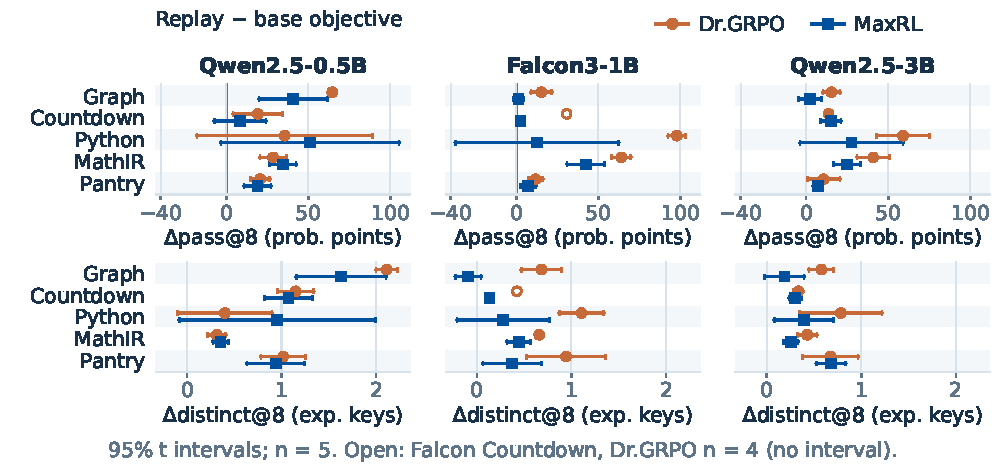
\includegraphics[width=\linewidth]{figures/replay_factorial_effects.pdf}
\caption{\textbf{Replay raises mean correctness at all three model scales.}
Final-checkpoint differences: Re:Dr minus Dr.GRPO (circles) and Re:Max minus
MaxRL (squares), measured in percentage points for \texttt{pass@8} and in
\pmd{} units for diversity. Filled markers use five paired seeds; hollow
markers use fewer. For Re:Dr, correctness uses four seeds in Falcon
\texttt{Countdown}; diversity uses four in Falcon \texttt{Countdown}, one
in Falcon \texttt{MathIR}, and two in Qwen2.5-3B \texttt{Python}. Diversity
requires at least 20 eligible prompts per arm; blanks indicate no eligible
comparison. Bars show nominal paired 95\% Student-$t$ intervals, requiring
five seeds for correctness and at least two for diversity.}
  \label{fig:replay-factorial-effects}
\end{figure}

\subsection{Terminal comparisons across scales}
\label{app:scale-matrix}
\label{app:scale-snapshot}
\label{app:maxrl-scale-extensions}
\label{app:current-campaign-results}

Paired conditions share initialization, training and evaluation prompts,
eight training passes, evaluation requests, the verifier, and replay schedule.
The control uses the same buffer construction and scoring procedures with
zero replay gradient. Policies can develop different buffers and workloads,
so total compute is not matched (App.~\ref{app:compute-matching}).

\crossscaletablematerial

\paragraph{Dr.GRPO retention contrasts.}
\label{app:retention-numerical-detail}

% Floats rather than [H] so it can rise to the page its discussion starts
% on instead of forcing a break and leaving the preceding page part empty.
\begin{table}[!tbp]
  \centering
  \caption{\textbf{Replay improves mean correctness and solution diversity at each tested scale.}
  Final-checkpoint differences between Re:Dr and Dr.GRPO, by domain and
  model. Superscripts indicate fewer than five paired seeds; dashes indicate
  no eligible comparison. Diversity effects require at least 20 eligible
  prompts per arm. Each Avg weights a fixed set of domains equally within
  seed: all five for correctness, and domains eligible for every seed for
  diversity. The diversity mean uses \texttt{Graph} and \texttt{PantryPlan}
  at Falcon3-1B, all domains except \texttt{Python} at Qwen2.5-3B, and all
  five at 0.5B. Eligible prompt subsets may differ between the two arms.}

\label{tab:cross-scale-terminal-effects}
  \scriptsize
  % Keep the two longest domain headers on two lines, as in the main table,
  % so typewriter labels retain their size within the thirteen-column layout.
  \setlength{\tabcolsep}{1.4pt}
  \renewcommand{\arraystretch}{0.92}
  \begin{tabular}{@{}l*{12}{r}@{}}
    \toprule
    & \multicolumn{6}{c}{\textbf{$\Delta$ \texttt{pass@8}}}
      & \multicolumn{6}{c}{\textbf{$\Delta$ \pmd{}}} \\
    \cmidrule(lr){2-7}\cmidrule(l){8-13}
    & \texttt{Graph} & \shortstack{\texttt{Count}\\\texttt{down}} & \texttt{Python} & \texttt{MathIR} & \shortstack{\texttt{Pantry}\\\texttt{Plan}} & Avg
      & \texttt{Graph} & \shortstack{\texttt{Count}\\\texttt{down}} & \texttt{Python} & \texttt{MathIR} & \shortstack{\texttt{Pantry}\\\texttt{Plan}} & Avg \\
    \midrule
    \input{results/retention_matrix_panel_a_table_body.tex}
  \end{tabular}
\end{table}

Tables~\ref{tab:core-terminal-endpoints} and~\ref{tab:cross-scale-terminal-effects}
report means for each condition and paired replay effects, respectively.
Adding replay to Dr.GRPO increases mean \texttt{pass@8} and \distk{} in
all 14 comparisons with five paired seeds; \distk{} increases in all 74
individual seed pairs. Because \distk{} also depends on correctness, we use
\pmd{} to measure diversity conditional on a correct response.

For Qwen2.5-0.5B, \texttt{Countdown} \texttt{pass@8} rises from $.480$ to
$.672$, with a \pmd{} gain of $+.480$ (95\% interval $[+.447,+.513]$).
\texttt{Python} correctness rises from $.172$ to $.528$, with a diversity
gain of $+.082$ ($[-.146,+.310]$). \texttt{MathIR} correctness rises from
$.512$ to $.796$, with a diversity gain of $+.017$ ($[+.003,+.031]$).
These are nominal Student-$t$ intervals over five paired training seeds,
without multiple-comparison adjustment. \texttt{Countdown}'s final \pmd{}
values are $.007$ for Dr.GRPO and $.487$ for Re:Dr. Its keys distinguish
computation routes, but these held-out evaluations do not track the survival
of particular routes discovered during training.

Fig.~\ref{fig:maxrl-factorial-scale-extensions} shows the results by domain.
Two-method effects use shared seeds; factorial interactions use seeds shared
by all four methods. Diversity comparisons additionally require enough
verified responses to estimate the conditional distribution.

% Not [H]: this plate is a full text-block tall, so forcing it here left the
% rest of the preceding page blank whenever it did not fit. Letting it float
% fills that page and keeps the plate near the text that cites it by number.
\begin{figure}[!htbp]
  \centering
  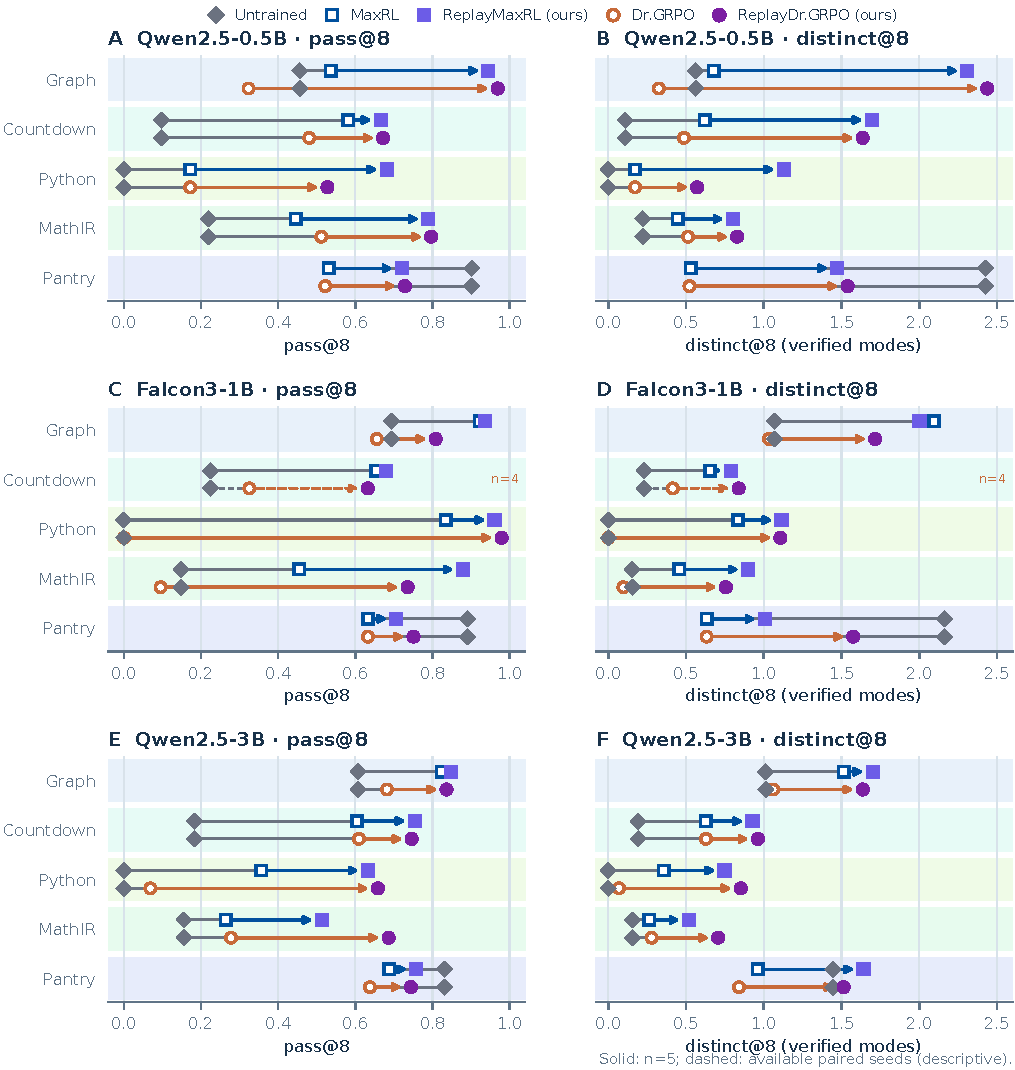
\includegraphics[width=.98\linewidth]
    {figures/e118_scale_extensions_appendix.pdf}
  \caption{\textbf{Replay gains vary by domain and model scale.}
  Final \texttt{pass@8} and \pmd{} at three model scales. Hollow and filled
  markers denote training without and with replay; circles denote Dr.GRPO,
  squares MaxRL, and gray diamonds the model before training. Correctness
  uses five paired seeds except Falcon \texttt{Countdown} Dr.GRPO ($n=4$).
  Diversity averages each arm's eligible seeds separately, requiring at least
  30 eligible prompts per seed. Lines are solid for five control seeds and
  dashed for fewer. Seed counts may differ between arms; estimates below the
  threshold are omitted. Table~\ref{tab:cross-scale-terminal-effects} reports
  paired diversity effects using a 20-prompt threshold. Error bars are omitted.}

  \label{fig:maxrl-factorial-scale-extensions}
\end{figure}


Diversity effects in Fig.~\ref{fig:replay-factorial-effects} and
Table~\ref{tab:cross-scale-terminal-effects} use paired seeds for which
both arms have at least 20 eligible evaluation prompts. The separate-arm
means in Table~\ref{tab:core-terminal-endpoints} and
Fig.~\ref{fig:maxrl-factorial-scale-extensions} instead require 30 eligible
prompts per seed in each arm. Correctness, absolute diversity, and paired
diversity effects can therefore use different seed sets; eligible prompt
subsets can also differ between arms. Diversity-effect intervals use
Student-$t$ with $n-1$ degrees of freedom for $n\ge2$ paired seeds; single-seed
effects have no interval. Correctness and mode-count intervals require five
paired seeds. All intervals are nominal 95\% estimates, without adjustment
for multiple comparisons.

For Qwen2.5-0.5B, Re:Max increases \pmd{} by $+.439$, $+.489$, and
$+.317$ on \texttt{Graph}, \texttt{Countdown}, and \texttt{PantryPlan},
respectively; each five-seed interval excludes zero. Falcon \texttt{Graph}
has a diversity effect of $-.009$ ($[-.034,+.016]$) and a correctness
effect of $+.014$ ($[-.016,+.044]$), both inconclusive. Thus a positive
cross-domain average does not imply improvement in every domain.

For Qwen2.5-3B, the five-seed \pmd{} effects are $+.076$, $+.077$,
$+.058$, $+.006$, and $+.224$ for \texttt{Graph}, \texttt{Countdown},
\texttt{Python}, \texttt{MathIR}, and \texttt{PantryPlan}, respectively.
All diversity intervals exclude zero, although the \texttt{MathIR} effect is
small. Correctness intervals exclude zero for \texttt{Countdown},
\texttt{MathIR}, and \texttt{PantryPlan}, but include zero for \texttt{Graph}
and \texttt{Python}. Across scales, Re:Max exceeds MaxRL in mean \pmd{} in
14 of 15 measurable comparisons; Re:Dr exceeds
Dr.GRPO in 14 of 14. These counts summarize
the signs of the estimated effects, not their statistical significance.

\paragraph{Cross-domain factorial summaries.}
\label{app:factorial-numerical-detail}
Weighting all five domains equally within each paired seed, Re:Max improves
\texttt{pass@8} over MaxRL by $+.307$ at Qwen2.5-0.5B (95\% interval
$[+.208,+.406]$), $+.133$ at Falcon3-1B ($[+.043,+.223]$), and $+.154$
at Qwen2.5-3B ($[+.086,+.222]$). Each comparison uses five seeds. The
corresponding Re:Dr effects are $+.337$, $+.442$, and $+.279$. The Falcon
Dr.GRPO comparison uses four common seeds and has no interval; the other
two use five.

At Qwen2.5-3B, MaxRL and Re:Max have mean correctness $.547$ and $.701$,
and mean \distk{} $.744$ and $1.107$, respectively. Their paired mode-count
difference is $+.363$ ($[+.285,+.441]$). The cross-domain \pmd{} means in
Table~\ref{tab:cross-scale-terminal-effects} use a fixed set of domains
eligible for every contributing seed.

\subsection{Level 1 at Qwen2.5-7B}
\label{app:qwen7b-level1}

We also compare MaxRL and Re:Max at Qwen2.5-7B on Level~1 in
3 domains. The 6 training runs form one
matched treatment--control pair per domain, each trained for
3072 updates with the same prompts, horizon, verifier,
evaluation procedure, and replay schedule as the smaller-scale comparisons.
With one matched seed per domain, these effects are descriptive and have no
confidence intervals.

On \texttt{MathIR}, MaxRL's observed \texttt{pass@8} reaches zero
at update 960 and remains zero at subsequent evaluations.
The final evaluation contains no verified response, so \pmd{} cannot be
estimated. Table~\ref{tab:qwen7b-level1} reports it as undefined rather than
zero. Re:Max, evaluated on the same prompts and seed, reaches
.744 \texttt{pass@8} and .017
\pmd{}. The correctness result remains measurable even though a paired
diversity effect is unavailable.

Where both conditions have measurable diversity, Re:Max increases \pmd{}
by +.298 on \texttt{Graph} and
+.137 on \texttt{Countdown}. These point estimates
exceed the corresponding 3B means, but one seed does not establish a trend
with model scale. Mean \texttt{pass@8} across all 3 domains
is .342 for MaxRL and .789 for Re:Max. Mean
\pmd{} is .028 and .245, respectively, over the
2 domains where both conditions define it. Thus the
correctness mean includes \texttt{MathIR}, while the diversity
mean does not.

\begin{table}[!htbp]
  \centering
  \caption{\textbf{Level-1 correctness and solution diversity at Qwen2.5-7B.}
  Results from 6 runs with 1 matched seed per
  domain after 3072 updates. On \texttt{MathIR},
  MaxRL produces no verified response: its correctness is zero, while its
  \pmd{} and the paired diversity effect are undefined (\texttt{--}).
  Means use 3 domains for correctness and the
  2 jointly eligible domains for diversity. No confidence
  intervals are reported per domain for these single-seed comparisons.}

  \label{tab:qwen7b-level1}
  \small
  \setlength{\tabcolsep}{6pt}
  \begin{tabular}{@{}l*{6}{r}@{}}
    \toprule
    & \multicolumn{2}{c}{\textbf{MaxRL}} & \multicolumn{2}{c}{\textbf{Re:Max}}
      & \multicolumn{2}{c}{\textbf{Re:Max $-$ MaxRL}} \\
    \cmidrule(lr){2-3}\cmidrule(lr){4-5}\cmidrule(lr){6-7}
    \textbf{Domain} & \texttt{pass@8} & \pmd{} & \texttt{pass@8} & \pmd{}
      & \texttt{pass@8} & \pmd{} \\
    \midrule
    \input{results/e124_qwen7b_level1_20260924_table_body.tex}
  \end{tabular}
\end{table}

\subsection{Results on harder benchmark levels}
\label{app:level2-interim}

\begin{figure}[!htbp]
\centering
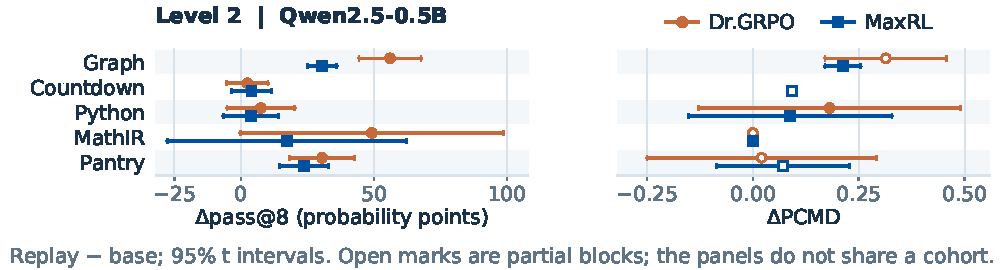
\includegraphics[width=\linewidth]{figures/replay_level2_effects.pdf}
\caption{\textbf{Replay improves Level-2 \texttt{Graph} accuracy and solution diversity.}
Final Re:Dr minus Dr.GRPO (circles) and Re:Max minus MaxRL (squares) effects
for Qwen2.5-0.5B, in percentage points of \texttt{pass@8} and \pmd{} units.
Correctness uses five paired seeds per domain. Diversity requires at least
20 eligible prompts per arm. Re:Dr uses three seeds for \texttt{Graph} and
\texttt{PantryPlan}, four for \texttt{MathIR}, and none for
\texttt{Countdown}; Re:Max uses one for \texttt{Countdown} and four for
\texttt{PantryPlan}. Other comparisons use five. Hollow markers indicate
fewer than five pairs; blanks indicate no eligible pair. Bars show nominal
paired 95\% Student-$t$ intervals for comparisons with at least two seeds.}

  \label{fig:replay-level2-effects}
\end{figure}

Fig.~\ref{fig:level2-admission} compares replay effects across Levels 1--3
using fixed domain sets. Correctness gives equal weight to \texttt{Graph},
\texttt{Countdown}, \texttt{Python}, and \texttt{PantryPlan} within each of
five common training seeds. Diversity first averages eligible seeds within
each arm and domain, then weights \texttt{Graph}, \texttt{MathIR}, and
\texttt{PantryPlan} equally. Its contributing seeds can differ across arms
and levels, so differences between these diversity means are descriptive
and have no intervals. At Level 2, only \texttt{PantryPlan} has sufficient
verified responses before training to estimate diversity; the initial
three-domain diversity mean is therefore undefined.

Each Level-2 method has five final training seeds per domain. The diversity
comparisons in Fig.~\ref{fig:replay-level2-effects} additionally require
eligible prompts in both arms. \texttt{Graph} improves under both objectives:
Re:Max increases \pmd{} by $+.212$ ($[+.170,+.255]$, five seeds), and
Re:Dr by $+.314$ ($[+.170,+.458]$, three seeds). The corresponding
\texttt{Python} effects are $+.088$ and $+.181$, with intervals including
zero; \texttt{MathIR} effects are near zero. \texttt{PantryPlan}
correctness improves by $+.305$ under Re:Dr and $+.237$ under Re:Max,
each measured over five seeds.

Each Level-2 \texttt{MathIR} prompt admits one shortest derivation and four
longer alternatives. Concentration on the shortest route therefore yields
near-zero diversity despite the existence of other valid modes. The levels
also use different held-out problems and can differ in mode-count
distributions and prompt guidance (App.~\ref{app:data-levels}). Cross-level
comparisons consequently do not isolate the causal effect of difficulty.

For each common seed and endpoint $Y$, the replay interaction is
\[
 I=(Y^{\rm Re:Max}-Y^{\rm MaxRL})
    -(Y^{\rm Re:Dr}-Y^{\rm Dr.GRPO}).
\]
A negative interaction means that replay adds less under MaxRL than under
Dr.GRPO; it does not imply that replay harms MaxRL. On Level-2
\texttt{Graph}, MaxRL alone improves \texttt{pass@8} over Dr.GRPO by
$+.233$ ($[+.140,+.325]$), while the replay interaction is $-.256$
($[-.329,-.183]$). Replay improves both objectives, with a smaller
additional benefit under the stronger fresh objective.

\begin{table}[!htbp]
  \centering
  \caption{\textbf{A stronger fresh objective need not increase the additional benefit of replay.}
  Contrasts use five common seeds per domain across all four methods.
  The interaction is
  $(\mathrm{Re:Max}-\mathrm{MaxRL})-(\mathrm{Re:Dr}-\mathrm{Dr.GRPO})$.
  Here $P_8=\texttt{pass@8}$, $D_8=\texttt{distinct@8}$, and $B_8=D_8-P_8$.
  Entries report paired means and nominal 95\% Student-$t$ intervals. Both
  mode-count metrics depend on correctness. The conditional-diversity analysis
  in Fig.~\ref{fig:replay-level2-effects} applies separate eligibility
  requirements, so its seed populations can differ from those in this table.}

\label{tab:level2-factorial-contrasts}
  \scriptsize
  \setlength{\tabcolsep}{3pt}
  \resizebox{\linewidth}{!}{%
  \begin{tabular}{@{}lclrrr@{}}
    \toprule
    \textbf{Domain} & $n$ & \textbf{Contrast} &
    $\Delta P_8$ & $\Delta D_8$ & $\Delta B_8$ \\
    \midrule
    \input{results/level2_factorial_contrasts_20260912_table_body.tex}
  \end{tabular}}
\end{table}


\paragraph{Level-2 \texttt{Graph} results.}
\label{app:levels-numerical-detail}
Before training, Qwen2.5-0.5B \texttt{Graph} \texttt{pass@8} is $.438$
on the Level-1 development split and $.148$ on Level 2. After eight Level-2
training passes, Dr.GRPO and MaxRL reach $.202$ and $.434$, compared
with $.763$ and $.739$ for Re:Dr and Re:Max. The paired correctness gains
are $+.561$ and $+.305$, with 95\% Student-$t$ intervals $[+.445,+.677]$
and $[+.250,+.360]$ over five seeds each. The lowest replay accuracy
($.711$) exceeds the highest accuracy without replay ($.477$). Replay adds
$1.019$ and $.668$ distinct verified modes for the two objectives,
respectively, yielding \texttt{distinct@8} of $1.243$ and $1.214$.

For the three eligible Dr.GRPO seed pairs, \pmd{} rises from $.039$ to
$.353$; for the five MaxRL pairs, it rises from $.112$ to $.325$.
Expressed on the effective-mode scale, these changes are $1.04$ to $1.55$
and $1.13$ to $1.48$, corresponding to ratios of $1.49$ and $1.32$.
Relative increases in \pmd{} are unstable near a zero baseline, so we
report absolute changes instead. The joint improvements in correctness and
diversity do not establish that greater diversity causes better correctness.

\subsection{Accuracy and verified modes throughout training}
\label{app:factorial-training-curves}

Figs.~\ref{fig:factorial-training-accuracy}--\ref{fig:level2-training-pmd}
show correctness and diversity throughout training, using four groups of
eight responses to each of 128 held-out prompts. Lines show seed means;
bands show the range across seeds, rather than confidence intervals. A seed
contributes to conditional diversity only when at least five prompts have
two or more correct responses. The contributing seeds and prompts can
therefore change across methods and checkpoints.

\begin{figure}[!htbp]
  \centering
  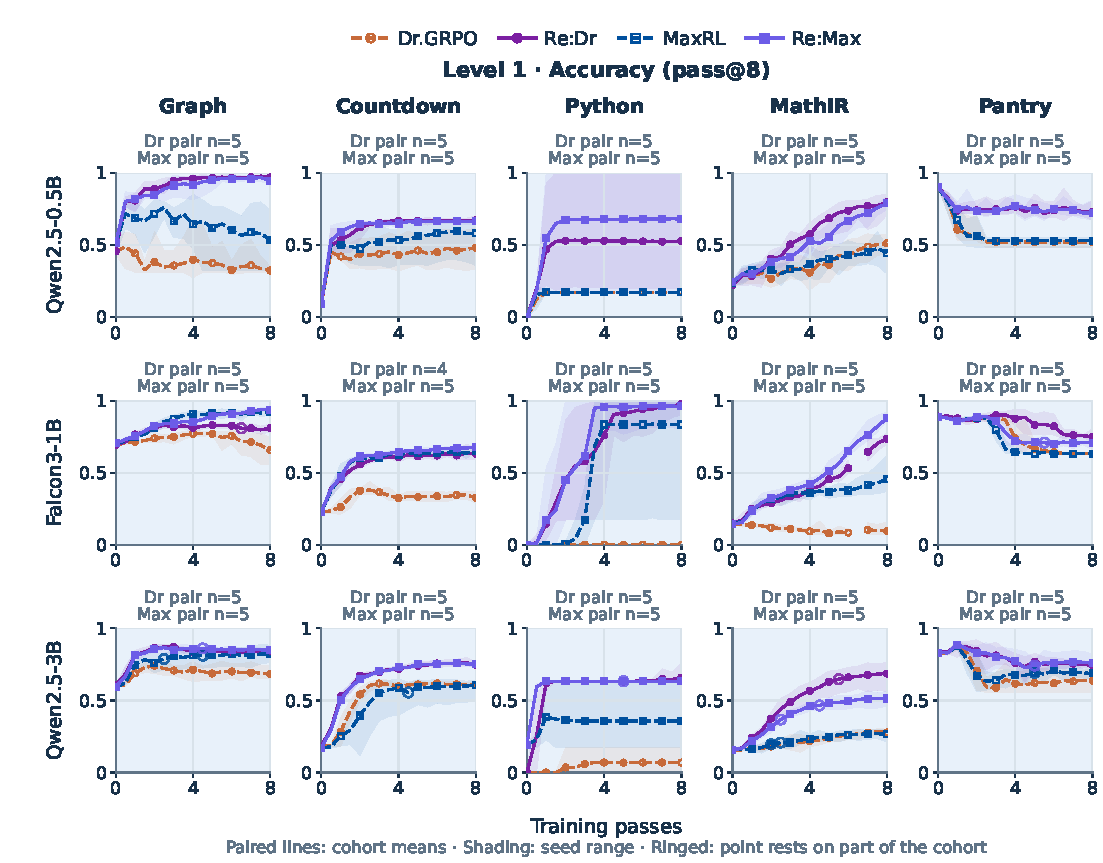
\includegraphics[width=\linewidth]{figures/factorial_training_curves_pass8.pdf}
  \caption{\textbf{Replay improves final accuracy across model scales.}
  \texttt{pass@8} over eight training passes for Dr.GRPO, Re:Dr, MaxRL, and
  Re:Max. Rows show Qwen2.5-0.5B, Falcon3-1B, and Qwen2.5-3B; columns show
  domains. Panel labels give the numbers of paired seeds at the final
  checkpoint. Lines show seed means and bands show seed ranges, rather than
  confidence intervals. Ringed points use fewer seeds than the final comparison.}

  \label{fig:factorial-training-accuracy}
\end{figure}

\begin{figure}[!htbp]
  \centering
  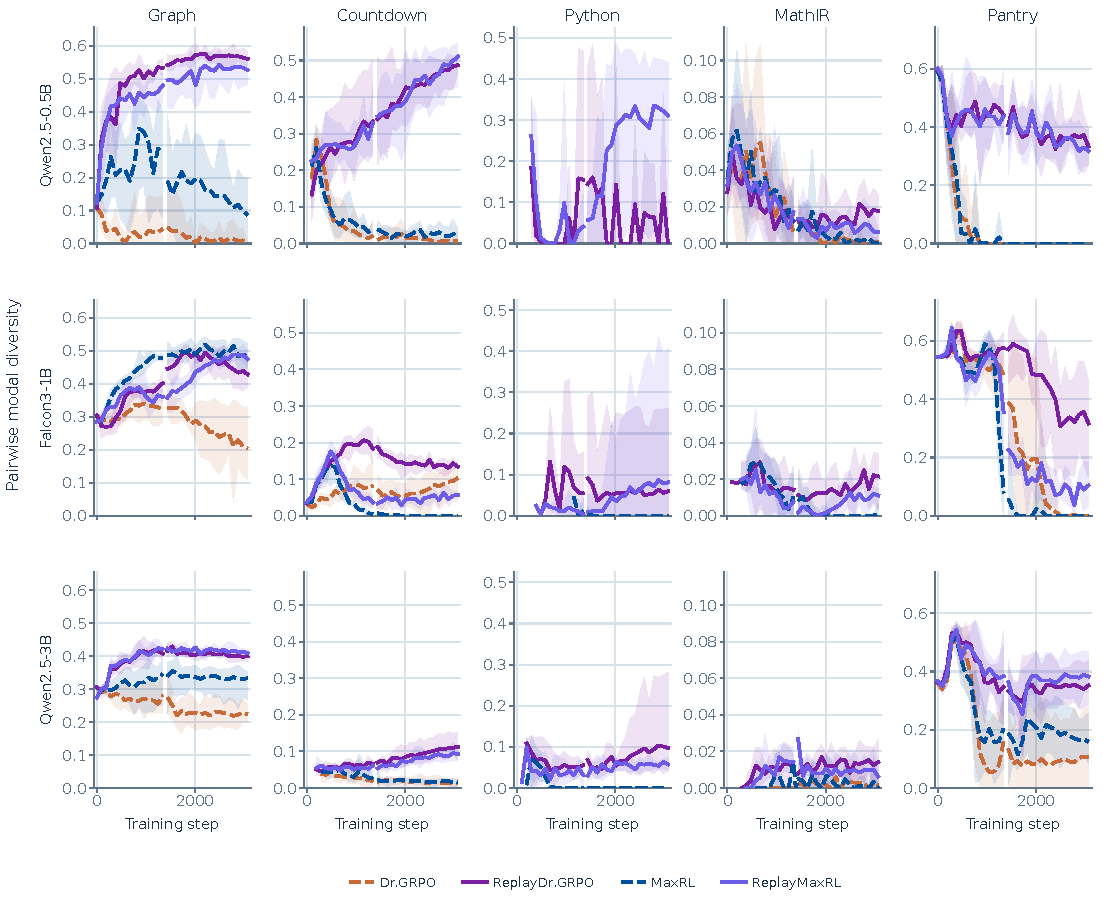
\includegraphics[width=\linewidth]{figures/factorial_training_curves_pmd.pdf}
  \caption{\textbf{Replay limits the loss of \texttt{PantryPlan} solution diversity at every scale.}
\pmd{} throughout training, with model rows and method colours as in
Fig.~\ref{fig:factorial-training-accuracy}. Both fresh objectives reach zero
terminal \texttt{PantryPlan} diversity at 0.5B and 1B, whereas both replay variants
retain multiple solution modes. Lines average one to five eligible seeds
per checkpoint; bands show seed ranges and are absent for a single seed.
A seed contributes when at least five prompts yield at least two correct responses.
Fine dotted segments use fewer seeds, so changes can reflect sample
composition. Gaps indicate undefined estimates. Vertical scales are shared
within each domain.}
  \label{fig:factorial-training-modes}
\end{figure}

\begin{figure}[!htbp]
  \centering
  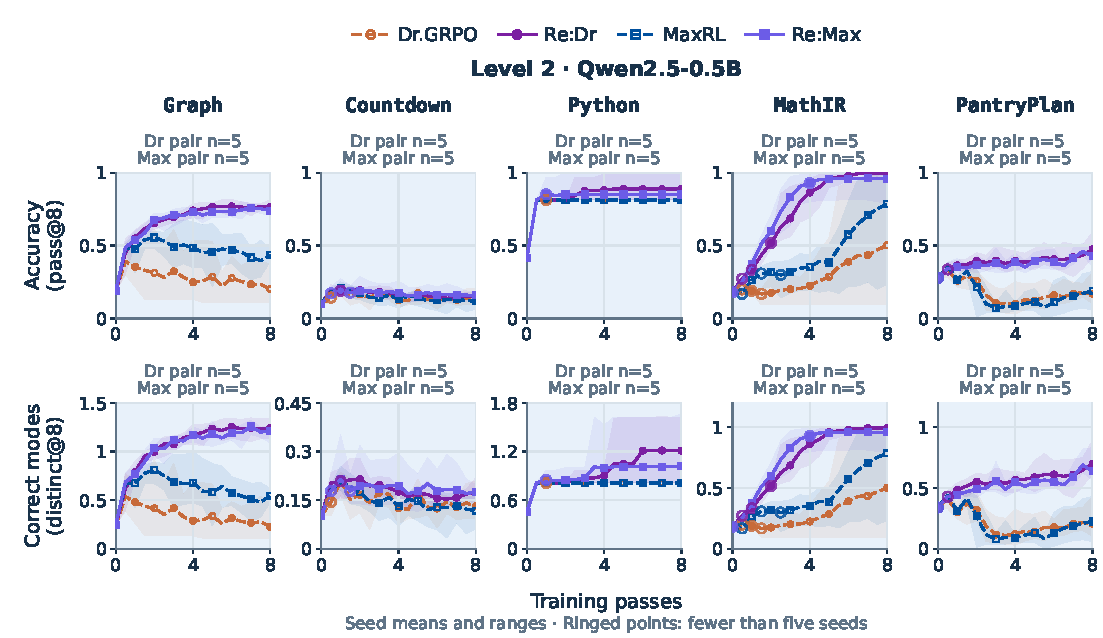
\includegraphics[width=\linewidth]{figures/level2_factorial_training_curves.pdf}
  \caption{\textbf{Replay improves final accuracy and verified-mode counts at Level~2.}
Qwen2.5-0.5B trajectories for Dr.GRPO, Re:Dr, MaxRL, and Re:Max across five
domains. Rows show \texttt{pass@8} and \distk{}; the latter depends on both
correctness and solution diversity. Each objective pair has five matched
seeds at the terminal checkpoint. Lines show seed means and bands show
seed ranges. Ringed points use fewer than five seeds; Fig.~\ref{fig:level2-training-pmd}
reports success-conditional diversity.}
  \label{fig:level2-training-curves}
\end{figure}

\begin{figure}[!htbp]
  \centering
  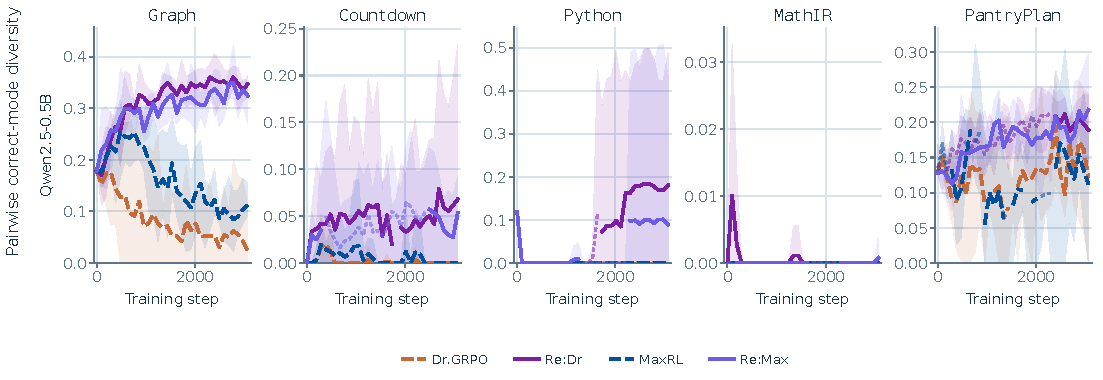
\includegraphics[width=\linewidth]{figures/level2_training_curves_pmd.pdf}
  \caption{\textbf{Replay preserves greater solution diversity on Level-2 \texttt{Graph}.}
\pmd{} during Qwen2.5-0.5B training for the four primary methods. At the
terminal checkpoint, Re:Dr and Re:Max reach $.346$ and $.325$, compared with
$.023$ for Dr.GRPO and $.112$ for MaxRL. \texttt{MathIR} remains near zero under all
four methods. Lines average eligible seeds and bands show seed ranges.
Each seed requires at least five prompts with at least two correct responses.
Fine dotted segments indicate fewer contributing seeds, and gaps indicate that the estimate is undefined.}
  \label{fig:level2-training-pmd}
\end{figure}


\subsection{Supporting comparators}
\label{app:ucpo-progress}

GRPO normalizes rewards within each group; UCPO redistributes the advantage
among fresh on-policy responses; sparse RLEP-Dr reuses verified successes
without uniform weighting by canonical key. We evaluate GRPO in 75 training
runs across three model scales. UCPO and RLEP-Dr cover the two smaller
scales, with 50 and 47 runs, respectively. RLEP-Dr uses two seeds for Falcon
\texttt{Python} and five elsewhere. Fixed Semantic-MaxEnt adds a
frequency-based bonus to fresh responses (App.~\ref{app:semantic-maxent}).
Its four-method factorial covers ten model--domain combinations at the two
smaller scales, with five common seeds except Falcon \texttt{Countdown}
($n=4$). The 3B comparison uses one seed to evaluate adding the bonus to
replay (App.~\ref{app:semantic-current-factorial}).

For GRPO, UCPO, and RLEP-Dr, the diversity contrasts in this subsection
average per-prompt differences over prompts with at least two correct
responses in both arms. Each seed must have at least 30 such jointly
eligible prompts. Table~\ref{tab:direct-comparator-matrix} instead uses
separate 20-prompt thresholds for each arm. On Qwen2.5-0.5B \texttt{Graph},
one UCPO seed and four RLEP-Dr seeds meet the joint criterion; no
\texttt{Python} comparison meets it at any scale.

For Qwen2.5-0.5B, UCPO improves \texttt{Countdown} \texttt{pass@8} by
$+.133$ ($[+.005,+.262]$), while its \pmd{} effect is inconclusive:
$+.002$ ($[-.018,+.023]$). Its \texttt{MathIR} effects are also
inconclusive. RLEP-Dr improves \texttt{MathIR} correctness by $+.126$
($[+.030,+.222]$), with zero measured diversity change; its
\texttt{Countdown} and Falcon \texttt{PantryPlan} effects are inconclusive.
Across GRPO, UCPO, and RLEP-Dr, seven of 34 five-seed correctness intervals
lie above zero. None of the 19 five-seed diversity intervals lies above zero; one lies
below zero, for Falcon \texttt{Countdown} GRPO: $-.105$
($[-.147,-.063]$). At Qwen2.5-3B, all five GRPO correctness intervals and
the three available diversity intervals include zero. These are nominal
paired 95\% Student-$t$ intervals over training seeds.

The uniform versus frequency-weighted replay comparison uses five paired
seeds in each of nine model--domain combinations: all five Qwen2.5-0.5B
domains, plus \texttt{Graph} and \texttt{PantryPlan} at both larger scales.
Changing only the within-buffer weights increases extra verified modes by
$+.318$ per prompt in the Qwen2.5-0.5B average ($[+.272,+.358]$,
paired-seed bootstrap). The correctness effect is inconclusive at $+.010$
($[-.119,+.139]$). This result supports a benefit from uniform weighting
beyond reusing successful responses in proportion to their frequency,
although extra-mode counts still depend on correctness
(App.~\ref{app:frequency-replay-progress}).

RLEP-Dr's offline response pool uses temperature $.7$ and top-$p=.95$;
evaluation uses temperature 1 and top-$p=1$. Its offline data collection
also differs from the online construction of prompt-specific verified replay
buffers, and the next paragraph measures what that difference puts in the pool.

\paragraph{What RLEP-Dr replays.}
\phantomsection\label{app:rlep-pool}
RLEP's protocol harvests its experience pool from a policy that RL has
already trained \citep{zhang2025rlep}: the seed policy samples 64 candidates
per prompt at temperature $.7$ and top-$p=.95$, verified answers are kept, and
a prompt enters the pool only with at least two of them. Here the seed policy
is the paired terminal Dr.GRPO control, so the pool is a sample from the
collapsed endpoint that Sec.~\ref{sec:results-collapse} measures.
Table~\ref{tab:rlep-pool-composition} reads the frozen pools and the learner
telemetry of every RLEP-Dr cell. At Qwen2.5-0.5B,
43\%--79\% of the 384 training prompts hold
no verified trajectory and never receive a replay row. Of the
4393 eligible prompts pooled over all 25
cells, all but 17 hold a single canonical key among
their verified trajectories, and none holds more than 2, so a
two-row replay draw is two copies of one mode with probability at least
.99 in every domain.
Falcon3-1B pools are slightly wider on \texttt{Graph} and \texttt{Countdown},
up to 1.40 keys per eligible prompt, and a same-mode pair
remains the draw with probability
.89--1.00. The online Re:Dr buffer on the
same prompts and seeds holds 2.6--6.9 modes on average
in the three domains where modes are plentiful. RLEP-Dr's replay is therefore
single-mode replay of the control's own endpoint, applied on
21\%--57\% of updates, and its \pmd{} beside the
control is the expected outcome rather than a discrepancy with Re:Dr: no
update rule rehearses a second mode from a pool that holds one.

The two update rules are closer than their descriptions suggest. RLEP's
replay row enters the policy gradient with advantage $1-\bar r$, where
$\bar r$ is the mean reward of the mixed group, so it is a positive-coefficient
log-likelihood term on a stored success, as Re:Dr's replay term is. The
difference is that RLEP's coefficient shrinks toward zero as the prompt is
solved, with a realized mean of .03--.38 across domains
at 0.5B, whereas Re:Dr's is fixed. Whether a likelihood term on a single
stored success can produce breadth is tested directly by the capacity-one arm
of App.~\ref{app:mode-agnostic-replay}, which applies exactly such a term to
one success captured online at first discovery and recovers 58\% of
the Re:Dr effect. What separates the two replay families is thus not the loss
but the buffer: what it stores, from which policy, and from when.

\begin{table}[H]
  \centering
  \caption{\textbf{RLEP-Dr's pools hold one mode per prompt.} Composition of
  the frozen RLEP experience pools and the realized replay dose, averaged over
  seeds. \emph{none} is the share of the 384 training prompts with no verified
  trajectory; \emph{eligible} the share with at least two; \emph{keys} the mean
  number of canonical modes among an eligible prompt's verified trajectories;
  $P(\text{same})$ the probability that a two-row replay draw repeats one
  mode; \emph{updates} the share of optimizer updates that mixed in replay
  rows; $A_{\text{replay}}$ the mean replay advantage $1-\bar r$ on those
  updates. The last column is the mean number of modes in the Re:Dr buffer
  over the within-cohort cells on the same prompts and seeds
  (Tab.~\ref{tab:matched-redr}).}
  \label{tab:rlep-pool-composition}
  \small
  \setlength{\tabcolsep}{5pt}
  \begin{tabular}{@{}lrrrrrrrr@{}}
    \toprule
    \textbf{Domain} & $n$ & \textbf{none} & \textbf{eligible} & \textbf{keys}
      & $P(\text{same})$ & \textbf{updates} & $A_{\text{replay}}$
      & \textbf{Re:Dr modes} \\
    \midrule
    \input{results/rlep_pool_composition_20260924_table_body.tex}
  \end{tabular}
\end{table}

\paragraph{Comparator settings.}
\phantomsection\label{app:comparator-settings}
Each comparator shares the non-objective settings of its paired control
(Table~\ref{tab:run-contract}). UCPO uses the published default
$\omega=.2$, and RLEP-Dr uses the published combination of 16 fresh and
2 replay responses. GAPO has no free coefficient; its reward is affinely
mapped to the control's unit range because Dr.GRPO does not normalize by
the group standard deviation. SetPO uses $\lambda=1.0$, giving a diversity
term approximately 5.3\% of the task advantage; its paper provides no
coefficient for the 0.5B verifier-reward setting. Semantic-MaxEnt uses
$\eta=.10$ and $\kappa=5$. Replay uses $\lambda_{\mathrm{replay}}=.10$
and capacity $M=16$, equal to the rollout group size. These settings are
not tuned to \mb{} outcomes, and no method receives a learning-rate sweep.
The results therefore compare the methods at the stated settings;
hyperparameter tuning could improve correctness or diversity.

\paragraph{Interpreting zero diversity.}
In Table~\ref{tab:direct-comparator-matrix}, an em-dash denotes an undefined
paired difference. An exact $.000$ instead denotes a measured zero, with
identical values for both methods in every eligible seed. The
\texttt{Python} \pmd{} column contains measured zeros because, for each
eligible prompt, both methods' verified responses share a single execution
key. High correctness can coexist with this concentration: four of the five
SetPO \texttt{Python} seeds reach \texttt{pass@8} $1.000$ and terminal
\pmd{} $.000$. Every held-out prompt has at least one correct response,
but the verified responses for each prompt use a single mode. Per-response
correctness also increases in all 15 control comparisons
(App.~\ref{app:control-learning-audit}).

\begin{figure}[!htbp]
  \centering
  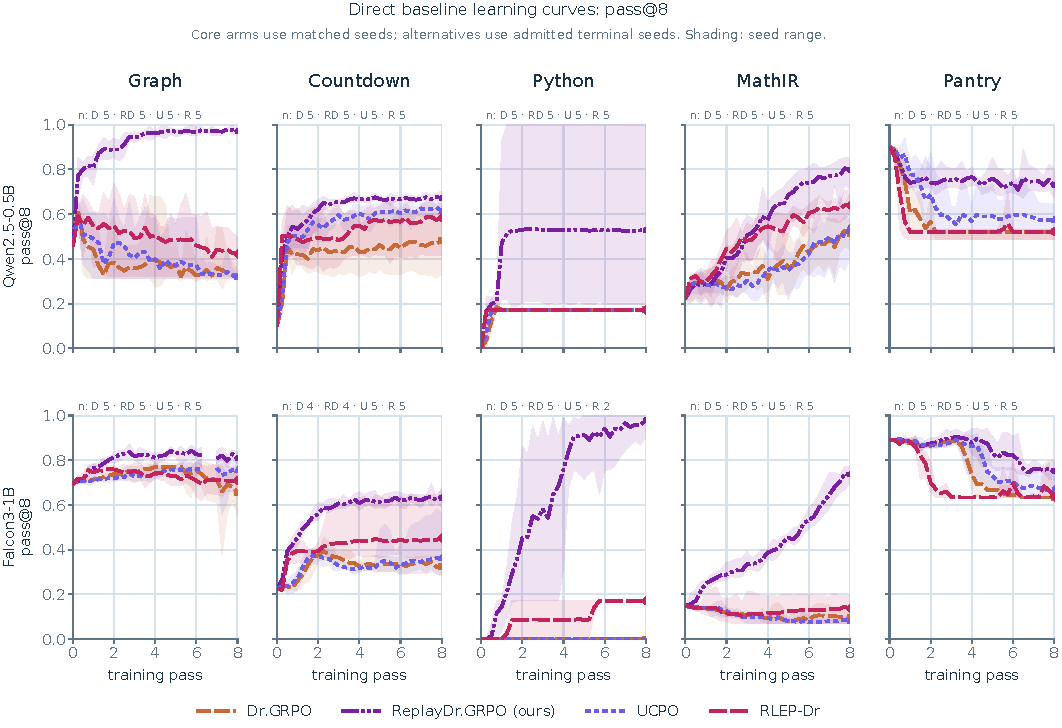
\includegraphics[width=\linewidth]{figures/direct_baseline_learning_curves_pass8.pdf}
  \caption{\textbf{Re:Dr has the highest terminal mean accuracy in every
  displayed comparison.} \texttt{pass@8} during Level-1 training for Dr.GRPO,
  Re:Dr, UCPO, and sparse RLEP-Dr. Rows show Qwen2.5-0.5B and Falcon3-1B;
  columns show the five domains. Lines show seed means and bands show seed
  ranges; gaps indicate unavailable estimates. Dr.GRPO and Re:Dr use paired
  seeds. Comparisons use five seeds except Falcon \texttt{Countdown}
  Dr.GRPO/Re:Dr ($n=4$) and Falcon \texttt{Python} RLEP-Dr ($n=2$), as indicated in the panels.}
  \label{fig:direct-baseline-accuracy-curves}
\end{figure}


\subsection{Diversity-preserving comparators}
\label{app:diversity-comparators}

GAPO~\citep{anschel2025groupaware} and SetPO~\citep{li2026setpo} target
output diversity within the fresh rollout group. Both are evaluated on
Level-1 Qwen2.5-0.5B across five domains and five seeds. GAPO assigns
verifier-positive rollouts the reward $[1-(f_i-1/L)+1]/2$, with zero for
failures, where $f_i$ is the key's frequency among the group's verified
rollouts and $L$ is the prompt's certified number of valid modes.
SetPO augments each rollout's advantage by its marginal contribution to
kernelized set diversity, measured by removing that rollout from the group,
with coefficient $\lambda=1$. It computes similarities using a fixed
\texttt{all-MiniLM-L6-v2} sentence encoder, mean pooling, and cosine
similarity clamped to $[0,1]$. Encoding the responses adds computation.

GAPO increases \pmd{} on \texttt{Countdown} ($+.340$, $[+.112,+.567]$) and \texttt{PantryPlan}
($+.653$, $[+.610,+.696]$), while its \texttt{Python} effect is near zero
with an interval spanning zero. \texttt{Python} has more valid modes than the
sixteen-rollout group can represent on 95\% of training prompts, with up to 3,600
modes. This limits within-group coverage but does not prevent a policy from
assigning mass across the full support. \texttt{MathIR} effects are small across
methods; the largest is Re:Dr's $+.017$ ($[+.003,+.031]$).
SetPO increases \pmd{} on \texttt{PantryPlan} ($+.266$, $[+.177,+.356]$); its other
four domain intervals include zero. Five-domain mean effects are $+.225$
for GAPO, $+.066$ for SetPO, and $+.320$ for Re:Max, although GAPO's
\texttt{PantryPlan} effect is larger than Re:Max's. The effective number
of modes, $\neff$, on \texttt{PantryPlan} is $2.88$ for GAPO and $1.36$
for SetPO, compared with $1.00$ for their shared control. SetPO also raises
\texttt{Python} \texttt{pass@8} from $.338$ to $.834$, a relative increase
of $147\%$. Relative changes in \pmd{} are undefined for \texttt{PantryPlan}
and \texttt{Python} because the control has $\pmd=.000$. GAPO adjusts
rewards using frequencies within the fresh rollout group, whereas replay
balances the likelihood term across verified modes accumulated in the buffer.

GAPO and SetPO share a Dr.GRPO control with matching hardware and
nonoverlapping evaluation draws. Its terminal \pmd{} differs from the
Dr.GRPO control used in the main replay comparison by a mean of $+.003$
over twenty paired comparisons, ranging from $-.014$ to $+.034$. These
observed differences are small relative to the five-domain effects above,
but do not establish equivalence between the controls.

\subsection{Measured KL tradeoffs and replay occupancy}
\label{app:kl-measured}

Table~\ref{tab:reference-kl-measured} compares terminal \pmd{} at
Qwen2.5-0.5B, Level~1, after $3{,}072$ updates. Dr.GRPO with reference KL
uses 6 coefficients, $\beta\in\{0.001, 0.01, 0.04, 0.1, 0.2, 0.3\}$, across
5 domains. These arms use the zero-replay-derivative control
configuration with a nonzero KL coefficient and the initial policy as the
reference. The comparisons match optimizer updates and fresh-rollout
budgets. They do not equalize total computation: reference-policy evaluation
and replay processing incur different costs, and the control does not spend
those costs on additional effective updates or fresh rollouts.

\begin{figure}[t]
  \centering
  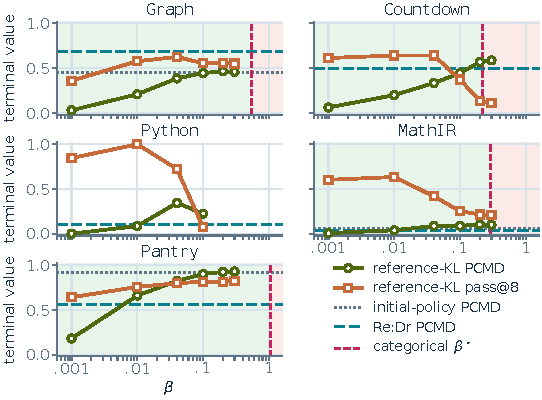
\includegraphics[width=0.78\linewidth]{figures/reference_kl_knee.pdf}
  \caption{\textbf{KL coefficient effects vary by domain.}
  Circles show terminal \pmd{} and squares show \texttt{pass@8} for
  Qwen2.5-0.5B at Level~1; lines connect seed means without uncertainty
  bands. Horizontal rules mark the initial policy's reportable \pmd{}
  (dotted) and Re:Dr's terminal \pmd{} (dashed). Vertical rules mark the
  categorical plug-in threshold $\beta^\star$; green and red indicate
  stationary single-draw correctness above and below one half under that
  calculation. This threshold does not predict the location of the observed
  \texttt{pass@8} knee.}
  \label{fig:reference-kl-knee}
\end{figure}

\paragraph{Initial concentration and coefficient dependence.}
Dr.GRPO without KL reaches \pmd{} at or below $.004$ in all five domains.
MaxRL without replay reaches $.148$ in \texttt{Graph} and at or below $.022$
elsewhere. These low values are consistent with concentration, but the
neural runs do not satisfy the independent-logit assumptions of
Proposition~\ref{thm:grpo-collapse}.
KL produces larger conditional-diversity estimates at several coefficients
in every domain. The response is not uniformly monotone: \texttt{Graph} changes
from $.465$ to $.458$ and \texttt{MathIR} from $.103$ to $.099$ between
$\beta=.2$ and $.3$, while \texttt{Python} changes from $.344$ to $.225$ between
$\beta=.04$ and $.1$.
These are comparisons of point estimates, without a seed-level uncertainty
analysis for their differences.

\begin{table}[t]
  \centering
  \caption{\textbf{KL and replay have different domain-level tradeoffs.}
  Terminal \pmd{} seed means for Qwen2.5-0.5B, Level~1. Superscripts give
  counts below five seeds; dashes indicate unavailable cells. The four
  zero-KL arms use 32 disjoint evaluation streams; KL arms use their own
  disjoint draws with the same estimator. Reference summaries are
  initial-policy \pmd{} and $1-1/\bar k$ for each replay arm, where $\bar k$
  is the mean number of keys replayed per measured update. These do not bound
  neural diversity. The final column computes categorical $\beta^\star$
  from mean initial single-draw correctness.}
  \label{tab:reference-kl-measured}
  \scriptsize
  \setlength{\tabcolsep}{2.5pt}
  \begin{tabular}{@{}lrrrrrrrrrrrrrr@{}}
    \toprule
    & \multicolumn{2}{c}{\textbf{without replay}}
      & \multicolumn{6}{c}{\textbf{$+$ reference KL, by $\beta$}}
      & \multicolumn{2}{c}{\textbf{$+$ replay}}
      & \multicolumn{3}{c}{\textbf{reference summaries}} & \\
    \cmidrule(lr){2-3}\cmidrule(lr){4-9}\cmidrule(lr){10-11}\cmidrule(lr){12-14}
    \textbf{Domain} & Dr.GRPO & MaxRL
      & $.001$ & $.01$ & $.04$ & $.1$ & $.2$ & $.3$
      & \textbf{Re:Dr} & \textbf{Re:Max}
      & Initial & Re:Dr & Re:Max & $\beta^\star$ \\
    \midrule
    \input{results/reference_kl_table_body.tex}
  \end{tabular}
\end{table}

\paragraph{Stationary predictions and measured checkpoints.}
Proposition~\ref{prop:kl-stationary} identifies the categorical interior
stationary conditional as $q^\star=\mu|_{\mathcal C}$, independently of
$\beta$. It does not bound transient diversity or establish that a finite
neural checkpoint reaches this conditional. The measured \pmd{} varies
with $\beta$ and can exceed the initial estimate: at $\beta=.2$, \texttt{Graph}
reaches $.465$ against $.454$ initially, \texttt{MathIR} $.103$ against $.061$,
and \texttt{Pantry} $.925$ against $.913$. These estimates also condition on each
policy's own verified responses, rather than on a common set of solved
prompts.

For a fixed prompt with $0<\mu(\mathcal C)<1/2$, the Dr.GRPO formula gives
\[
  \beta^\star=\frac{(G-1)/G}{-\operatorname{logit}\mu(\mathcal C)},
  \qquad P^\star(\beta^\star)=\tfrac12.
\]
The displayed values substitute each domain's mean initial correctness
and $G=16$, giving $0.22$--$1.05$.
This aggregation is descriptive: substituting a mean into the nonlinear
stationary formula does not give the mean of its promptwise predictions.
Moreover, $P^\star$ is single-draw correctness, whereas the plotted
\texttt{pass@8} measures success within eight responses. Declines in that
metric already occur below the displayed threshold: \texttt{MathIR} falls from
$.634$ at $\beta=.01$ to $.418$ at $.04$, well below its
$\beta^\star\simeq.29$. \texttt{Countdown} similarly falls from $.642$ at $.04$
to $.372$ at $.1$, below $.22$. The thresholds therefore do not locate
the measured knees. \texttt{Python} has zero observed initial successes, so no
finite plug-in threshold or reportable initial \pmd{} is shown; this
does not establish zero population correctness.

Finite training, shared parameters, prompt sampling, and the adaptive
optimizer can all separate the measured neural trajectory from the
categorical stationary calculation. The comparison does not identify their
individual effects. The boundary-force identities and the two-mode
$\Theta(1/[s\log(1/s)])$ versus $\Theta(\log(1/s))$ recovery result
characterize their stated categorical models, not measured neural recovery
rates.

\paragraph{What buffer occupancy measures.}
For a nonempty fixed uniform categorical buffer with $k$ keys, the limiting
diversity is $1-1/k$. Across such buffers,
$\E[1-1/k]\le1-1/\E[k]$ by Jensen's inequality. The table instead uses
$\bar k$, the number of keys replayed per measured update, averaged within
runs and then across seeds. Buffers change during training, and updates
without replay can contribute zero keys. Thus $1-1/\bar k$ is a
descriptive transform of training occupancy, not an estimate of the
nonempty fixed-buffer expectation in that inequality. Neither quantity
bounds held-out neural \pmd{}.

\texttt{Python} illustrates a possible discovery difference. Re:Max averages
$1.73$ replayed keys per update against Re:Dr's $1.18$, while terminal
\pmd{} is $.239$ versus $.099$. Corollary~\ref{cor:maxrl-starvation}
provides a categorical motivation for stronger fresh learning when
correctness is scarce, but these measurements do not isolate discovery
from prompt weighting, sampling, or optimization. Occupancy also does not
order all outcomes: in \texttt{Countdown}, Re:Max has fewer replayed keys per
update ($2.10$ versus $2.28$) but higher \pmd{} ($.531$ versus $.497$).
In \texttt{Pantry} both arms average about $6.7$ keys and reach about $.557$ \pmd{}.
The capacity of 16 keys would allow a uniform fixed-buffer value of
$1-1/16=.9375$; the occupancy summary near $.85$ is not that capacity
limit and does not prove why KL performs better there.

\paragraph{Observed correctness--diversity comparisons.}
In \texttt{Python} and \texttt{Pantry}, at least one measured KL coefficient exceeds both
replay arms on \pmd{} and has no lower \texttt{pass@8} point estimate.
In \texttt{Countdown} and \texttt{MathIR}, coefficients that exceed both replay arms on
\pmd{} have lower \texttt{pass@8} than both. In \texttt{Graph},
all measured coefficients are below both replay arms on both metrics.
These comparisons concern seed means; they establish neither statistical
dominance nor a ranking at equal total compute.
\paragraph{Relative and absolute readings of the Re:Max effect.}
Table~\ref{tab:reference-kl-measured} carries both arms of the Re:Max versus
Dr.GRPO comparison on one evaluation, so the effect can be read either way.
Equally weighting the five domains, Dr.GRPO reaches \texttt{pass@8} $.405$ and
Re:Max $.772$, a relative increase of $90\%$; averaging the five per-domain
relative increases instead gives $124\%$, because \texttt{Python} rises from a
small base. A relative reading of \pmd{} is not available: terminal Dr.GRPO
\pmd{} is $.000$--$.004$ across these domains and exactly $.000$ in
\texttt{Python} and \texttt{PantryPlan}, so two of the five ratios are
undefined and the rest are dominated by the denominator. The count-valued
reading is well defined instead. Re:Max reaches $\neff$ of $2.66$, $2.13$,
$1.32$, $1.02$ and $2.25$ on \texttt{Graph}, \texttt{Countdown},
\texttt{Python}, \texttt{MathIR} and \texttt{PantryPlan}, against
$1.00$--$1.004$ for Dr.GRPO: a mean ratio of $1.87$ effective verified modes
for each one the control retains. Paired per-seed \pmd{} differences on a
common eligible population, which weight prompts and seeds differently, are
reported in Table~\ref{tab:direct-comparator-matrix}.

Figure~\ref{fig:reference-kl-plane} averages \texttt{Graph}, \texttt{MathIR}, and
\texttt{Pantry}, the three domains with reportable initial \pmd{}, across all
six coefficients. Between $\beta=.2$ and $.3$, mean \pmd{} changes from
$.498$ to $.496$, while \texttt{pass@8} changes from $.527$ to $.528$.

\subsection{Reference quality, discovery, and the scope of the comparison}
\label{app:kl-case}

\paragraph{Reference quality can favor KL.}
A full-support fixed reference yields the full-support categorical
stationary policy in Proposition~\ref{prop:kl-stationary}. Reference KL
uses that policy rather than a replay buffer; it requires reference-policy
evaluation but no rule for admitting exemplars. In \texttt{Pantry} at
$\beta=0.3$, the 5-seed mean reaches
$\pmd{}=0.931$ and \texttt{pass@8} $0.825$.
The replay arm with larger \pmd{} reaches $0.557$ and
$0.797$, respectively. \texttt{Pantry}'s initial \pmd{} is
$0.91$, consistent with a useful reference conditional.
The measurements support reference quality as one possible explanation;
they do not show that replay's capacity or discovery alone causes the
difference.

\paragraph{Reference diversity varies across evaluation populations.}
App.~\ref{app:hosted-mode-diversity} reports 7
hosted deployments with macro \pmd{} spanning 0.14--0.31;
Kimi K3 is highest at 0.31. Of
101 reportable model--domain--level cells,
7 reach $.50$ and the maximum is
$0.74$. These estimates are lower than \texttt{Pantry}'s initial
$0.91$ in the local comparison, but the models,
evaluation populations, and reportability sets differ. The hosted cohort
therefore describes additional candidate reference distributions; it does
not establish how training with those references would perform. Under the
categorical proposition, each reference determines a stationary
conditional, not a ceiling on a retrained neural policy. Replay instead
targets the solution modes represented by its discovered buffer.

\paragraph{Correctness costs depend on the domain and coefficient.}
The largest observed \texttt{pass@8} reduction among KL cells that exceed
both replay arms on \pmd{} occurs in \texttt{MathIR} at
$\beta=0.3$. Its 5-seed mean is
$0.099$ \pmd{} and $0.207$ \texttt{pass@8},
compared with $0.039$ and $0.816$ for
the replay arm with larger \pmd{}. This finite-checkpoint comparison
supports a domain-dependent correctness--diversity tradeoff, without
identifying the categorical threshold as its cause.
Replay's positive dose does not change its full-coverage categorical
limit under Corollary~\ref{cor:replay-no-collapse}, only the rate at which
that limit is approached. A measured
replay-dose sweep would be needed to compare coefficient sensitivity.

\paragraph{Limits of the evidence.}
Reference \pmd{} requires at least 30 defined prompts in an initial
evaluation. This eligibility condition affects which policy conditionals
can be compared. \texttt{Python}'s zero observed initial correctness cannot
support an inheritance explanation for its measured KL gains.
\texttt{MathIR}'s support certificate counts derivations and does not imply
that a policy will produce every certified solution mode.

The categorical results separate a fixed-reference target from a
discovered-buffer target and characterize restoration under their stated
assumptions. The neural measurements compare finite checkpoints. They do
not establish a universal preference between KL and replay, a discovery
cause for every replay shortfall, or an advantage under equal total compute.

\subsection{Uniform versus fresh-frequency replay}
\label{app:frequency-replay-progress}

The weighting ablation uses the same buffer construction and update rule,
changing only the within-buffer target: uniform weights over retained keys
versus weights proportional to verifier-positive fresh-rollout counts.
The resulting policies can produce different buffer contents during training.
Positive contrasts below favor uniform weighting. We report
$B_8=\texttt{distinct@8}-\texttt{pass@8}$, extra verified modes per prompt,
and $P_8=\texttt{pass@8}$. The five-domain Qwen2.5-0.5B aggregate averages
domain effects within each matched seed, giving equal domain weight.

Paired-seed intervals enumerate all $5^5=3{,}125$ ordered bootstrap
resamples of the five paired training seeds and use linearly interpolated
2.5th and 97.5th percentiles. Each resampled seed carries its complete domain
vector for the five-domain aggregate. These nominal intervals quantify seed
variability within the fixed benchmark; prompts and domains are not resampled,
and intervals are not adjusted across comparisons.

The Qwen2.5-0.5B five-domain effect is $+.318$ extra modes per
prompt ($[+.272,+.358]$), with positive within-seed domain averages in all
five seeds. \texttt{Graph}, \texttt{Countdown}, and \texttt{PantryPlan} drive this result; \texttt{Python} and
\texttt{MathIR} remain inconclusive. The $P_8$ effect is $+.010$
($[-.119,+.139]$), establishing neither a gain nor equivalence. \texttt{Python}'s
$P_8$ effects range from $-.781$ to $+.828$ across seeds despite
small extra-mode effects in four seeds.

Falcon3-1B \texttt{Graph} also favors uniform weighting on extra modes ($+.233$,
$[+.182,+.320]$). Its correctness measures differ: $\Delta P_8=+.045$
($[-.0004,+.0910]$) is inconclusive, while the effect on mean per-response
correctness is negative at $-.0152$ ($[-.0214,-.0090]$).
Falcon3-1B \texttt{PantryPlan} is inconclusive on both outcomes:
$\Delta B_8=-.146$ ($[-.564,+.414]$) and $\Delta P_8=-.021$
($[-.063,+.026]$). Qwen2.5-3B \texttt{Graph} has five pairs and an extra-mode effect of
$+.079$ ($[+.011,+.135]$); its $P_8$ interval includes zero.
Qwen2.5-3B \texttt{PantryPlan} also has five pairs, with $\Delta B_8=+.207$
($[+.038,+.377]$) and inconclusive $\Delta P_8$ ($+.011$, $[-.020,+.043]$).

Rehearsing self-generated verified successes is related to rejection-sampling
fine-tuning~\citep{dong2023raft}; here the likelihood term is length-normalized
and combined with the on-policy objective. This ablation isolates the effect
of uniform versus fresh-frequency weighting within that replay procedure.
Uniform weighting increases extra verified modes in several domains.
The inconclusive $P_8$ effects do not establish that weighting leaves accuracy
unchanged or that replay's accuracy and diversity effects have separate causes.

\begin{figure}[H]
\centering
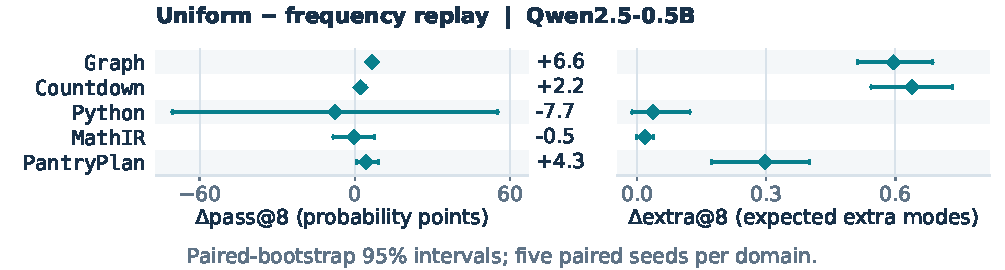
\includegraphics[width=\linewidth]{figures/replay_key_weighting.pdf}
\caption{\textbf{Uniform weighting preserves more verified alternatives.}
Uniform minus frequency-weighted replay at Qwen2.5-0.5B, Level 1, with five matched seeds. Extra modes are $B_8=\texttt{distinct@8}-\texttt{pass@8}$. Bars show nominal 95\% paired-seed bootstrap intervals. The mean gain is $.318$ extra modes, with an inconclusive correctness effect. Extra modes remain coupled to correctness; they do not measure success-conditional \pmd{}.}
\label{fig:replay-key-weighting}
\end{figure}

\input{results/semantic_current_summary_20260912.tex}

\newpage
\section{Concentration and Replay Mechanisms}
\label{app:ablations}

\input{results/fresh_concentration_20260912_appendix.tex}

\input{results/conditional_concentration_20260912_appendix.tex}

\begin{figure}[!htbp]
  \centering
  % One float, two panels: the same contrast read along the scale axis and
  % along the level axis. Equal minipage widths and matched native plate
  % widths, so neither panel is magnified relative to the other.
  \begin{minipage}[t]{.49\linewidth}
    \centering
    \textbf{(A)}\\[1pt]
    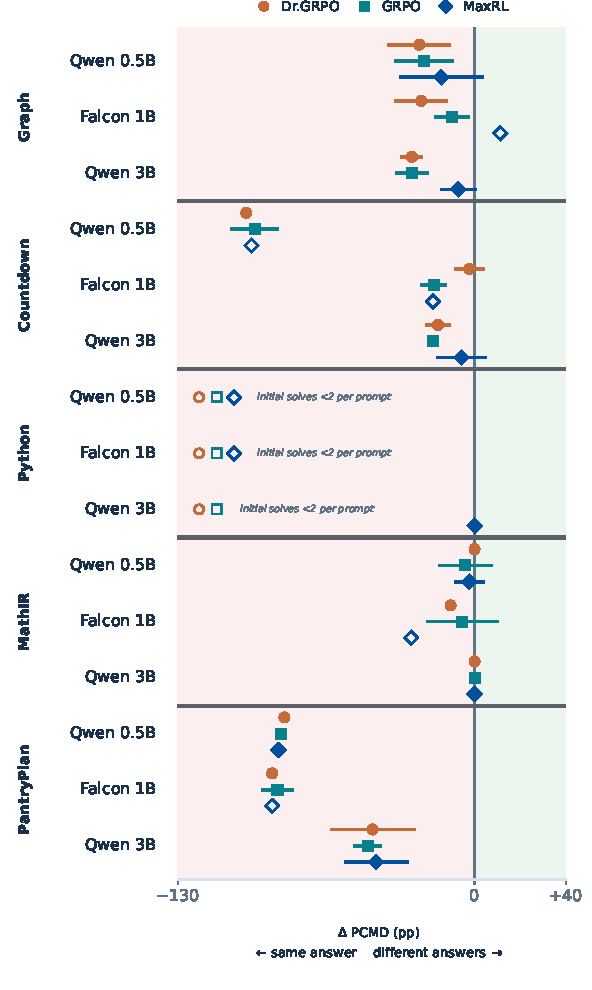
\includegraphics[width=\linewidth]{figures/concentration_story_all_scales.pdf}
  \end{minipage}\hfill
  \begin{minipage}[t]{.49\linewidth}
    \centering
    \textbf{(B)}\\[1pt]
    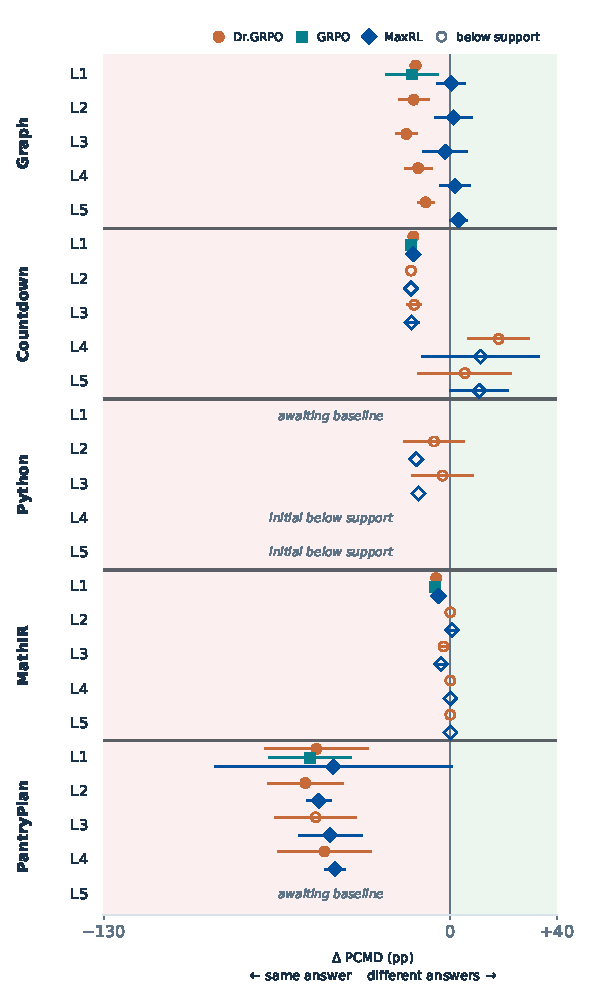
\includegraphics[width=\linewidth]{figures/concentration_levels.pdf}
  \end{minipage}
  \caption{\textbf{\texttt{Graph} and \texttt{PantryPlan} lose conditional solution diversity
  across scales and task levels.} Changes in \pmd{}, in percentage points.
  \textbf{(A)} Initial-to-final changes at Level~1 across three model scales
  and three objectives. Each seed averages over prompts with at least two
  correct responses at both checkpoints. Filled marks and bars show five-seed
  means and nominal paired 95\% Student-$t$ intervals. Open marks show
  means from fewer than five seeds, without intervals; annotated hollow
  symbols identify methods with no jointly eligible prompts. Dr.GRPO and GRPO reduce
  diversity in \texttt{Graph} and \texttt{PantryPlan} at every scale.
  \textbf{(B)} Level-1-trained policies evaluated on Levels~1--5, with
  Levels~2--5 measuring transfer. Available evaluations are averaged within
  each scale, then scales receive equal weight. Evaluations with different
  context limits contribute separately within a scale but do not constitute
  additional training seeds. Each scale uses one initial checkpoint evaluation.
  Bars appear only when one scale contributes and give nominal 95\%
  Student-$t$ intervals over its training seeds. Open marks indicate that at
  least one contributing scale has fewer than 30 eligible initial prompts or
  fewer than 30 eligible trained prompt observations in total. Missing initial
  references have fewer than two eligible prompts. GRPO appears only at
  Level~1. \texttt{Graph} and \texttt{PantryPlan} means decrease at every level; \texttt{Countdown}
  increases at Levels~4--5.}
  \label{fig:concentration-all-scales}
  \label{fig:concentration-levels}
\end{figure}


\subsection{Diversity before and after RLVR-only training}
\label{app:pre-rl-regression}

We evaluate Dr.GRPO and GRPO before training and after eight passes across
three models and five domains. The 150 runs each use four $K=8$ response
groups per checkpoint. Averaged equally across the five domains, extra
verified modes decrease by $98.2\%$--$99.4\%$ at Qwen2.5-0.5B and
$41.5\%$--$71.6\%$ at larger scales. The \texttt{pass@8} mean falls in
10 of the 30 domain--method--scale comparisons, while macro
\texttt{distinct@8} ends above its initial value at Qwen2.5-3B.
Fewer extra verified modes can therefore coexist with a greater probability
of sampling at least one correct response. Finite samples do not establish
that unobserved solution keys have zero probability.

\begin{samepage}
The domain average of \pmd{} includes only domains measurable at both endpoints: \texttt{Graph}, \texttt{MathIR}, and
\texttt{PantryPlan} at 0.5B; \texttt{Graph}, \texttt{Countdown}, and \texttt{PantryPlan} at 1B; and \texttt{Graph} and
\texttt{PantryPlan} at 3B. It declines by $98.5\%$ and $99.7\%$ at Qwen2.5-0.5B under
GRPO and Dr.GRPO, respectively, and by $50.8\%$--$65.1\%$ at the larger
scales. Terminal macro \pmd{} rounds to $.001$ for Dr.GRPO at Qwen2.5-0.5B.
The decline thus also appears in diversity conditional on success. Because
eligibility depends on the number of correct samples, these descriptive
averages do not hold the prompt population or correctness fixed.
App.~\ref{app:conditional-concentration} reports contrasts on jointly eligible
prompts. The decline is not universal: Falcon3-1B \texttt{Countdown} has
increasing \pmd{} under Dr.GRPO, from an initial value of $.033$.

\end{samepage}

Although the initial weights are shared, each method uses its own evaluation
samples. Differences between initial estimates therefore reflect sampling
variability.

\begin{figure}[t]
  \centering
  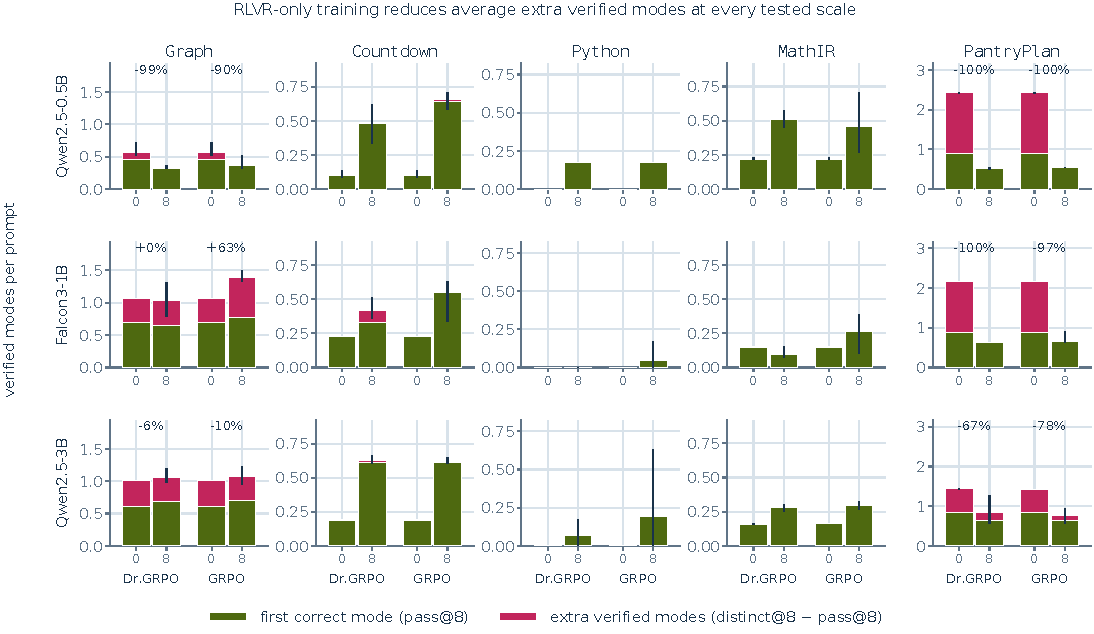
\includegraphics[width=\linewidth]{figures/baseline_collapse_precheck.pdf}
  \caption{\textbf{RLVR-only training reduces average extra verified modes
  at every tested scale.} Bars decompose \texttt{distinct@8} into
  \texttt{pass@8} and extra verified modes before training and after eight
  passes. Panels show Dr.GRPO and GRPO across three models and five domains:
  150 runs, with five seeds per model--domain--method combination and four
  eight-response groups per checkpoint. Whiskers show seed ranges; each
  method uses its own initial evaluation. Percentage changes in extra modes
  are shown for \texttt{Graph} and \texttt{PantryPlan}, whose initial means
  exceed $.05$. The other three domains start at $.011$ or less.}
  \label{fig:baseline-precheck}
\end{figure}




\texttt{Graph} and \texttt{PantryPlan} have substantial initial diversity at every
scale, whereas the other domains start with at most $.011$ extra modes per
prompt. To avoid unstable ratios near zero, retained-diversity percentages
are reported only when the initial extra-mode count exceeds $.05$.
The final $\texttt{distinct@8}$ is below its initial value in six of the
15 Dr.GRPO model--domain combinations. For Re:Dr, this occurs in two
available comparisons, both on \texttt{PantryPlan}; Falcon3-1B
\texttt{Countdown} uses four seeds. Conditional diversity comparisons
also depend on which prompts yield enough correct responses.
App.~\ref{app:conditional-concentration} reports paired contrasts on
jointly eligible prompts, including seed counts and uncertainty. These
held-out evaluations do not track individual modes stored during training.

Uniform sampling over the enumerable action representations gives a
diversity reference for \texttt{Graph} and \texttt{PantryPlan}
(App.~\ref{app:metric-sampling}). No corresponding reference is specified
for the other domains. On \texttt{PantryPlan}, uniform sampling of bit
masks yields higher expected \texttt{distinct@8} than the final sampled
value of every model under both Dr.GRPO and Re:Dr.

\begin{table}[t]
  \centering
  \caption{\textbf{Uniform actions and untrained checkpoints provide absolute diversity references.}
  \emph{Uniform} gives expected \distk{} under uniform sampling of the
  action representation: 27 color strings for \texttt{Graph} and 64 bit masks
  for \texttt{PantryPlan}. \emph{Initial} gives the Dr.GRPO pass-0 reference;
  the final two columns give sampled means after eight training passes.}
  \label{tab:absolute-support-references}
  \scriptsize
  \setlength{\tabcolsep}{4.2pt}
  \begin{tabular}{@{}llrrrr@{}}
    \toprule
    \textbf{Model} & \textbf{Domain} & \textbf{Uniform} & \textbf{Initial}
      & \textbf{Dr.GRPO} & \textbf{Re:Dr} \\
    \midrule
    \input{results/absolute_support_references_table_body.tex}
  \end{tabular}
\end{table}


\subsection{Vanishing task gradients and repeated outputs}
\label{app:degenerate-groups}

A Dr.GRPO group with identical rewards has exactly zero fresh task gradient.
Only mixed groups, containing both correct and incorrect responses,
provide a nonzero task advantage. Optimizer momentum can still change the
policy when the current task gradient is zero. The table below reports
the fraction of mixed groups over 3,072 Qwen2.5-0.5B updates, averaged
across five seeds.

\begin{center}
\small
\begin{tabular}{@{}lrr@{}}
\toprule
\textbf{Domain} & \textbf{Dr.GRPO} & \textbf{Re:Dr} \\
\midrule
\texttt{Graph} & .144 & .954 \\
\texttt{Countdown} & .140 & .456 \\
\texttt{Python} & .015 & .185 \\
\texttt{MathIR} & .364 & .453 \\
\texttt{PantryPlan} & .123 & .789 \\
\bottomrule
\end{tabular}
\end{center}

Thus 98.5\% of \texttt{Python} control updates carry zero fresh task gradient.
Replay contributes a likelihood gradient from verified responses and can
also change the policy so that subsequent fresh groups contain both correct
and incorrect responses.

All five Qwen2.5-0.5B \texttt{Python} control seeds exhibit observed output collapse.
At pass 0, eight-response groups average 7.99 distinct completion strings
per prompt. By steps 288--480, all 32 temperature-1 responses for each
prompt are identical within each seed and match its greedy completion.
This holds on all 128 prompts and persists at every subsequent evaluation
through step 3,072. The 32 responses span four groups with overlapping sampling
streams (App.~\ref{app:conditional-concentration}); they are not 32 independent
draws. Within eight-response groups, the terminal mean is 1.00 distinct
completion per prompt for the control and 1.97 for replay. The repeated
completion can be incorrect. These finite observations do not rule out
low-probability alternatives.

This sparse binary-reward setting allows fresh task gradients to vanish.
Sampling strategies that favor mixed groups, larger groups, a reference-policy
KL penalty, token-entropy regularization, or broader decoding could change
this behavior. The present comparison does not isolate their effects.

\subsection{The controls learn at the fixed learning rates}
\label{app:control-learning-audit}

The controls use a constant learning rate of $2\times10^{-7}$ at
Qwen2.5-0.5B and Falcon3-1B and a peak rate of $10^{-7}$ with cosine decay
at Qwen2.5-3B (Table~\ref{tab:run-contract}). Learning rates are not swept.
Table~\ref{tab:control-learning-audit} reports changes in accuracy and the
frequency of informative response groups under these schedules. The
results characterize the tested settings without identifying an optimal
schedule for either method.

\begin{table}[t]
  \centering
  \caption{\textbf{Per-response accuracy increases in every control comparison,
  while \texttt{pass@8} can fall.} Accuracy compares initial and last
  available evaluations. Columns show unpaired five-run means for each
  model--domain combination. \texttt{mean@8} measures per-response
  correctness. Mixed gives the mean fraction of rollout groups
  containing both correct and incorrect responses. An unmixed group has
  zero fresh task advantage, although optimizer momentum can still change
  the policy. Training schedules match update counts and fresh-rollout
  budgets; total compute is discussed in App.~\ref{app:compute-accounting}.}
  \label{tab:control-learning-audit}
  \small
  \setlength{\tabcolsep}{5pt}
  \begin{tabular}{@{}llrrrrrrr@{}}
    \toprule
    & & \multicolumn{3}{c}{\textbf{control \texttt{pass@8}}}
      & \multicolumn{2}{c}{\textbf{control \texttt{mean@8}}}
      & \textbf{mixed} & \textbf{Re:Dr} \\
    \cmidrule(lr){3-5}\cmidrule(lr){6-7}
    \textbf{Model} & \textbf{Domain} & initial & terminal & $\Delta$
      & initial & terminal & groups & \texttt{pass@8} \\
    \midrule
    \input{results/control_learning_table_body.tex}
  \end{tabular}
\end{table}

\paragraph{Accuracy changes during training.}
Per-response correctness (\texttt{mean@8}) rises in all 15
control comparisons: every control learns under its schedule. What varies
is coverage. Using an absolute-change threshold of $.005$, 8 of the
15 comparisons improve in \texttt{pass@8} and
6 decline, so 7 controls gain per-response accuracy
without a \texttt{pass@8} increase above that threshold. The mean
\texttt{pass@8} change is +0.039; the largest increase is $+0.426$
(\texttt{Countdown} at Qwen2.5-3B) and the largest decrease is $-0.380$
(\texttt{PantryPlan} at Qwen2.5-0.5B). In \texttt{PantryPlan} at Falcon3-1B, per-response correctness rises from
0.318 to 0.633, while \texttt{pass@8}
falls from 0.891 to 0.633.
This combination is consistent with prior observations of increased
single-response accuracy alongside reduced sampling coverage
\citep{yue2025rlvrlimit}.

The gap between \texttt{pass@8} and \texttt{mean@8} is at least $.02$ in
12 initial model--domain comparisons and below $.02$ in
7 terminal comparisons. This gap reflects variation in
correctness within response groups; it does not identify repeated strings
or conditional diversity among correct solution keys. The completion-string
analysis in App.~\ref{app:degenerate-groups} directly measures repetition
for the Qwen2.5-0.5B \texttt{Python} controls.

\paragraph{Sparse fresh reward information.}
Initial \texttt{pass@8} is zero on \texttt{Python} at all three
scales. In \texttt{Python} at Falcon3-1B, only a fraction 0.009 of
updates contain mixed rewards, leaving zero fresh task advantage in
99.1\% of updates. A learning-rate change cannot make an
identically zero current task gradient nonzero, but it can change the effect
of informative updates, optimizer momentum, and subsequent sampling.
The Falcon3-1B \texttt{Python} control's terminal \texttt{pass@8} rounds to $.000$, while Re:Dr
ends at $.979$. This is an accuracy contrast in a sparse-success setting;
conditional mode diversity requires at least two correct responses per
prompt and is undefined when that sampling condition is unmet.

\paragraph{Scope of the comparison.}
Replay and control share the learning rate, schedule, initialization,
prompt stream, optimizer, update count, and fresh-rollout budget.
The comparison measures the effect of replay under these settings.
Per-response correctness increases in the controls, but the absence of a
learning-rate sweep limits conclusions about their optimal performance.
Other learning rates could change accuracy, diversity, and the relative
benefit of replay; the present results do not determine those changes.

The frequency of mixed groups helps characterize these comparisons.
When a control rarely produces mixed groups (App.~\ref{app:degenerate-groups}),
replay provides a likelihood gradient on updates with no fresh task advantage.
We therefore also summarize replay effects in subsets with increasing
control accuracy. Across all 15 model--domain combinations, the mean
Re:Dr minus Dr.GRPO effect is $+.352$ in \texttt{pass@8} and $+.189$
in \pmd{}. Among the 9 combinations with any positive initial-to-final
change in control \texttt{pass@8}, the effects are $+.379$ and $+.118$.
Among the 6 that also have nonzero initial \texttt{pass@8} and at least
10\% mixed rollout groups, they are $+.247$ and $+.136$. Every comparison
in these subsets has positive effects on both metrics; the smallest effects
in the six-comparison subset are $+.137$ in \texttt{pass@8} and $+.013$
in \pmd{}. Its mean diversity effect is about two thirds of the mean
across all comparisons. Table~\ref{tab:control-learning-audit} gives the
control measurements that define these subsets.

\subsection{Likelihood changes with a fixed replay buffer}
\label{app:fixed-bank-survival}

We examine the likelihoods of stored responses during Qwen2.5-0.5B Re:Dr
training on \texttt{Graph}, using five seeds. The buffer contents and counts
of fresh verified responses are held fixed from immediately before the
fresh rollout at step 384. Uniform replay continues through step 3,072
without adding modes. For each stored exemplar, identified by prompt and
canonical mode, we measure mean token log probability $s$ and sequence
log probability $\ell$ whenever it is replayed. Changes compare its first
and final replay visits after the buffer is fixed; these steps can differ
across exemplars.

The 3,406 exemplars span 1,575 seed--prompt pairs, with 8--9 replay visits
per exemplar.
The pooled median change is $+.038$ nat/token (95\% interval
$[+.025,+.048]$), while the 10th percentile is $-.256$ and $2.61\%$ of
exemplars lose more than $.5$ nat/token ($[1.54,3.77]\%$).
The largest observed intermediate decrease is $-1.328$ nat/token. Sequence log
probability has median change $+.154$ nat/sequence ($[+.104,+.198]$),
with $21.99\%$ of exemplars losing more than $.5$ nat/sequence.
Lengths range from 4 to 100 tokens, so the token and sequence thresholds
measure different changes.

\begin{figure}[!htbp]
  \centering
  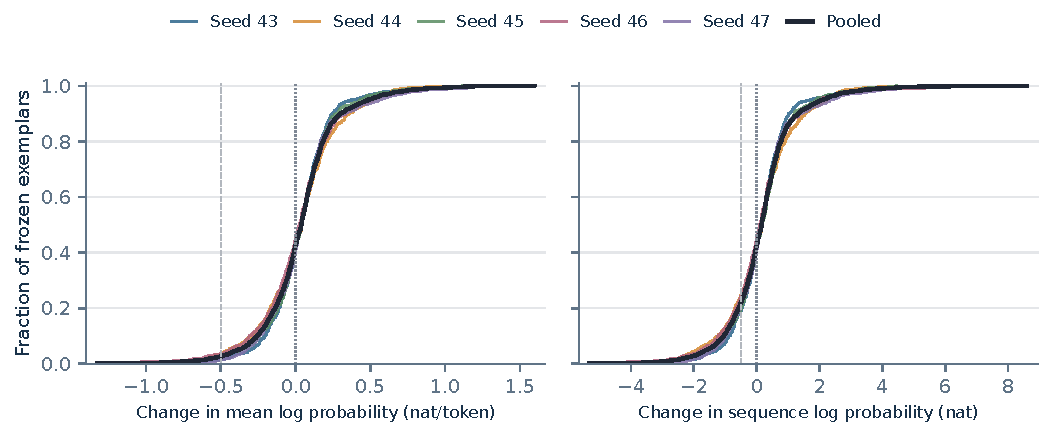
\includegraphics[width=.95\linewidth]{figures/e121_fixed_bank_survival.pdf}
  \caption{\textbf{Median exemplar scores rise, while some exemplars decline.}
  Empirical cumulative distributions of first-to-final score changes for
  3,406 fixed-buffer exemplars from five Qwen2.5-0.5B Re:Dr \texttt{Graph} seeds.
  Panels show mean token and sequence log probability. Colored curves
  represent individual seeds; the pooled curve weights exemplars equally.
  Dotted and dashed vertical lines mark zero and $-.5$, respectively.
  Positive changes indicate higher likelihood for the stored token sequence.
  Sequence likelihood does not measure the total probability of generating
  a canonical solution mode.}
  \label{fig:e121-fixed-bank-survival}
\end{figure}

Pooled summaries weight exemplars equally. Descriptive 95\% percentile
intervals use 10,000 hierarchical bootstrap replicates, resampling prompts
with replacement within each training seed and then resampling the five
seeds with replacement.

Scores are measured at replay visits, so changes between visits are
unobserved. Some stored exemplars lose likelihood despite continued replay.
A matched fixed-buffer control without replay would be needed to isolate
the effect of replay. These sequence-level observations also do not test
the mode-probability floor in Theorem~\ref{thm:replay-retention}.

\clearpage
\phantomsection
\begin{center}\large\textbf{Part IV. What diversity represents}\end{center}
\addcontentsline{toc}{part}{Part IV. What diversity represents}

\section{Matched Prompt-Hint Ablation}
\label{app:prompt-hint-ablation}

\input{results/modebench_prompt_ablation_20260911.tex}

\paragraph{Scope of the wording intervention.}
The \texttt{Python} intervention removes an executable nested-conditional example
along with divisor-testing and dispatch guidance, and it shortens the prompt.
Its effect concerns this combined change; it does not isolate a preference
cue from example or length effects. Lower \texttt{distinct@8} together with
lower \texttt{pass@8} can reflect reduced correctness rather than increased
concentration among correct outputs. The \pmd{} columns in
Table~\ref{tab:prompt-hints-local-strict} measure conditional diversity on
jointly eligible checkpoint--problem groups. Eligibility itself depends on
correctness, so these comparisons do not hold the full evaluation population
or its accuracy fixed.

\paragraph{Observed prompt dependence.}
\texttt{Python} shows a large loss of correctness after guidance removal. Across the
five Dr.GRPO seeds, mean $P_8$ falls from $.8125$ to zero at Level~2 and from
$1.0$ to zero at Level~3; $D_8$ falls identically and $B_8=0$ in both arms.
With no correct neutral Dr.GRPO outputs, its concentration among correct outputs
is undefined. Re:Dr retains neutral $P_8=.55625$ and $.49375$ and
$D_8=.675$ and $.65625$ at Levels~2 and~3, respectively, while losing
extra verified modes: $\Delta B_8=-.2375$ and $-.25625$. The initial checkpoint
also loses \texttt{Python} correctness (Table~\ref{tab:prompt-hints-local-strict}).
These observations identify substantial dependence on the combined \texttt{Python}
wording intervention; a raw mode-count decline cannot be interpreted solely
as a redistribution among correct answers.


\paragraph{\texttt{Python} responses after hint removal.}
Across 5,120 Dr.GRPO \texttt{Python} responses from five seeds, two levels, and both
wordings, all 2,560 outputs generated with the original wording yield the
same extracted lambda expression, whose body matches the conditional
example in the prompt; 2,320 of these
responses pass verification:
\begin{quote}\footnotesize\ttfamily
lambda n: 2 if n \% 2 == 0 else 3 if n \% 3 == 0 else 5
\end{quote}
\begin{samepage}
Of the 2,560 neutral-wording responses, 1,816 (70.94\%) are invalid Python
expressions, 59 violate other restricted-language rules, 376 return
non-integers, 276 fail the proper-divisor condition, and 33 (1.29\%) have
no extracted candidate after reaching the token limit. Syntax errors are
the largest failure category. The categories follow the first rejection
during extraction, parsing, and execution. They describe output failures
without identifying the training mechanism responsible.

\end{samepage}

\paragraph{Concentration after hint removal.}
Every trained \texttt{MathIR} checkpoint has $B_8=0$ under both wordings at both levels.
Within each problem's eight-draw group, every observed pair of correct
outputs shares a canonical key at every trained checkpoint and level:
correct-pair collision is $1.0$, versus the
uniform reference of $.2$ over five certified modes.
Table~\ref{tab:prompt-hints-local-strict} reports \pmd{} $.000$ under both
wordings in every eligible \texttt{MathIR} comparison. Removing this hint therefore leaves
observed correct outputs concentrated. At Level~2, Re:Dr retains mean $P_8=.975$ without the order hint, compared with $.99375$
with it. Across its five checkpoints, the neutral arm has 4,179 colliding
pairs out of 4,179 correct pairs, from 154 eligible checkpoint--problem
groups; the original arm has 4,382 out of 4,382 pairs from 157 such groups.
Both arms evaluate the same 32 problems at each checkpoint. Thus observed concentration persists after removing the order hint.
The comparison does not measure unseen modes, and the remaining interface
constraints still apply.
\texttt{PantryPlan} effects are mixed. Re:Dr at Level~3 gains $.109375$ in $D_8$,
comprising $.046875$ in $P_8$ and $.0625$ in $B_8$, but this comparison has only
two training seeds. App.~\ref{app:sampling-budget-ablation} evaluates
hosted models under both wordings with 64 draws on sixteen problems per
domain--level combination. Its problem population and sampling budget
differ from the eight-draw evaluation here.


\section{Decoding Temperature, Nucleus, and Budget}
\label{app:decoding-objection}

\paragraph{Temperature at fixed checkpoints.}
Qwen2.5-0.5B Dr.GRPO and Re:Dr checkpoints after eight training passes are
evaluated at $T\in\{.5,.7,1.0,1.3,1.6,2.0\}$, with top-$p=1$ and four
eight-response groups per prompt. Five domains, two methods, and five seeds
give 300 checkpoint--setting evaluations (Fig.~\ref{fig:decoding-objection}A).
The prompt template, evaluation split, response limit, and sampling seeds
are fixed across temperatures. Correct keys are pooled across response
groups for each prompt; the groups have overlapping sampling streams
(App.~\ref{app:conditional-concentration}). Estimates therefore describe
these sampled pools. A seed contributes to the \pmd{} mean when at least
30 prompts yield at least two correct responses. Eligible prompts and seeds
can differ across temperatures and methods.

Across the six temperatures, the largest control \pmd{} is $.021$ in
\texttt{Graph}, $.016$ in \texttt{Countdown}, $.002$ in \texttt{MathIR}, and $.004$ in \texttt{PantryPlan}.
Re:Dr at $T=1$ has corresponding means $.562$, $.485$, $.020$, and $.330$.
These four domains retain five eligible control seeds at every temperature.
\texttt{Python} controls have no seed reaching the 30-prompt threshold, so their
conditional diversity is unidentified under this reporting rule.
The sweep therefore shows low measured control diversity in the four
eligible domains, without establishing that unobserved modes have zero
probability or that every decoding choice would behave the same way.

\paragraph{Hardware sensitivity.}
All evaluations in the temperature sweep use NVIDIA RTX A5000 GPUs.
A paired comparison of A100 and A5000 evaluations at $T=1$ gives mean
absolute \pmd{} difference $.0032$ across twelve comparisons, with maximum
$.0131$. These differences describe the tested hardware comparisons;
they do not bound hardware sensitivity at other checkpoints or settings.

\paragraph{Larger groups and nucleus truncation.}
A separate set of Qwen2.5-0.5B checkpoints trained for twelve passes is evaluated at
eleven settings (Fig.~\ref{fig:decoding-objection}B): the six temperatures
above; two groups of $K=32$ at $T\in\{1.0,1.3,1.6\}$; and four groups
of $K=8$ with top-$p=.95$ at $T\in\{1.0,1.6\}$. The $K=32$ settings
quadruple the group size and double total responses per prompt from 32 to
64. Five domains, two methods, and five seeds give 550 checkpoint--setting
evaluations. The replay variant combines separate mass and within-buffer
balancing terms with novelty and semantic-entropy shaping. Its objective
and training duration therefore differ from the eight-pass Re:Dr comparison.

Control \pmd{} is zero throughout the grid in \texttt{Graph}. Its range is $.006$
to $.031$ in \texttt{Countdown}, $.000$ to $.003$ in \texttt{MathIR}, and $.037$ to $.069$
in \texttt{PantryPlan}.
All eleven settings retain five eligible control seeds in these domains;
\texttt{Python} controls remain below the reporting threshold. The replay markers
provide a descriptive reference for this separate variant, without
identifying the effect of the Re:Dr objective.

Three comparisons hold temperature and nucleus sampling fixed while
increasing both group size and total response budget: $K=8$ and $K=32$ at
$T\in\{1.0,1.3,1.6\}$, top-$p=1$. Across these matched settings, control
\pmd{} changes by at most $.010$ in absolute value, and no
$K=32$ control mean exceeds $.054$. \texttt{Graph} stays at $.000$;
\texttt{Countdown} moves from $.014$--$.027$ to $.013$--$.023$;
\texttt{MathIR} from $.000$--$.001$ to $.001$--$.003$; and \texttt{PantryPlan}
from $.050$--$.063$ to $.045$--$.053$. Each mean uses five eligible seeds.
The larger budget therefore does not move these controls out of their
low-\pmd{} range. This compares sampled pools at fixed checkpoints; it does
not establish that unobserved modes carry zero probability.

\begin{figure}[t]
  \centering
  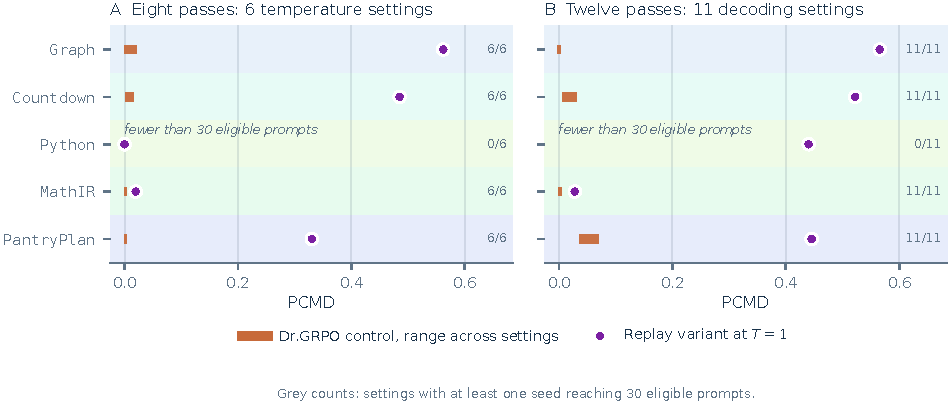
\includegraphics[width=\linewidth]{figures/decoding_objection.pdf}
  \caption{\textbf{Control diversity remains low across the tested decoding
  settings.} Qwen2.5-0.5B terminal \pmd{} across five domains.
  \textbf{(A)} Eight-pass Dr.GRPO/Re:Dr checkpoints at six temperatures
  ($T=.5$--$2.0$): 300 checkpoint--setting evaluations.
  \textbf{(B)} Separate twelve-pass checkpoints at eleven temperature, group-size,
  and nucleus settings: 550 evaluations, using a different replay objective.
  Bars span control means across settings; they are not confidence intervals.
  Markers show the corresponding replay variant at $T=1$, top-$p=1$,
  and $K=8$. Means use seeds with at least 30 prompts having at least two correct
  responses, so control and replay populations need not match. Control bars
  use five seeds outside \texttt{Python}; \texttt{Python} controls have none, while its replay
  markers use two seeds in A and three in B. Counts give eligible settings.
  Ranges narrower than $.004$ are displayed at width $.004$ for visibility.}
  \label{fig:decoding-objection}
\end{figure}

\paragraph{Scope of the decoding comparison.}
Both grids evaluate fixed terminal policies at one model scale. They do not
measure the effects of changing rollout temperature, optimizer settings, or
training duration. Correctness and conditional eligibility can change with
decoding settings; a missing \pmd{} estimate indicates insufficient eligible
prompts, rather than disappearance of all correct solution modes.

\section{Sampling-Budget Ablation}
\label{app:sampling-budget-ablation}

\input{results/modebench_discovery_curves_20260911.tex}

\input{results/discovery_hosted_interpretation_20260912.tex}

\input{results/gpt56_all_levels32_sampling_20260913.tex}

\subsection{Discovery at larger sampling budgets}
\label{app:sampling-budget-effects}

The 64-draw comparison in App.~\ref{app:sampling-budget-ablation} uses
36,864 responses from hosted models and 110,592 from Qwen checkpoints,
147,456 in total. Each of the six hosted model--wording combinations
contributes 6,144 responses. The Qwen evaluation includes 25 checkpoints:
each trained checkpoint is evaluated in its training domain at Levels~2
and~3, and the initial checkpoint covers all six domain--level combinations.
Every response remains in its sampling denominator. Formatting normalization
adds no verified Qwen responses, so both grading rules yield identical
estimates for these checkpoints. The sixteen problems per domain and level
differ from the thirty-two used in the 512-draw study
(App.~\ref{app:gpt56-all-levels-discovery}).

\paragraph{Prompt weighting changes the diversity summary.}
Tables~\ref{tab:discovery-breadth-frontier} and~\ref{tab:discovery-breadth-local}
compare two summaries of the 64-response pools. Within each checkpoint or
deployment, collision $C$ pools correct pairs across prompts, weighting each
prompt in proportion to $\binom{c}{2}$. Promptwise \pmd{} gives equal weight
to each prompt with at least two verified responses. Trained-checkpoint
scores then receive equal weight across seeds. Across 70 defined
combinations of model, domain, level, and wording, the median absolute
difference between promptwise \pmd{} and $1-C$ is $.003$, but nineteen
differ by at least $.05$.

For the initial checkpoint under original wording,
Level-2 \texttt{PantryPlan} has $1-C=.151$ and promptwise \pmd{} of $.587$;
Level~3 has $.625$ and $.307$, respectively. Both estimates use seven of
sixteen problems. The direction of the difference depends on which prompts
supply the most correct pairs and therefore receive the largest weights.

Neither weighting holds overall accuracy or the eligible population fixed.
For the initial checkpoint, Level-3 \texttt{Python} has sixteen eligible
problems under original wording and one under neutral wording. Each wording's
absolute estimate uses its own eligible prompts; paired differences use
only jointly eligible prompts. Equal prompt weights therefore describe
conditional diversity within these selected populations
(App.~\ref{app:metric-sampling}).

\paragraph{\texttt{MathIR}: concentration largely persists through 64 draws.}
At Level~2, both trained methods have $B_k=0$ at every measured budget under
both wordings. Re:Dr has $P_8=.9774$ and $P_{64}=.9875$ under original
wording, compared with $.9767$ and $.9875$ under neutral wording. Its $D_k$
equals $P_k$ throughout, so the small increase comes entirely from first
successes. At a budget of eight correct draws, both wordings have $R_8=1$
on the same 76 eligible checkpoint--problem pairs, compared with the
uniform lower reference $5[1-(4/5)^8]=4.1611$ from certified support.
These pairs reuse the same 16 problems across five checkpoints.

At Level~3, both trained methods under neutral wording and Re:Dr under
original wording also yield at most one correct key per checkpoint and
problem. Dr.GRPO under original wording has one exception: one checkpoint--problem
pair contains two keys with counts 28 and 9. Averaging over seeds and problems
gives $B_{64}=.0125$ and $B_{64}-B_8=.0035$. The corresponding equal-seed
correct-pair collision is $.9803$; the other trained \texttt{MathIR}
conditions have collision $1.0$, against the uniform upper reference $.2$.
The larger budget thus reveals a rare additional mode, precluding an exact
single-mode description of every trained condition.

\paragraph{\texttt{Python}: prompt dependence and additional discovery coexist.}
Under original wording, Dr.GRPO has $P_k=D_k=.8125$ at Level~2 and $1.0$
at Level~3 throughout the range from eight to 64 draws. Under neutral wording,
it has zero correct responses out of 5,120 at Level~2 and three out of
5,120 at Level~3. Each success is the only correct response for its
checkpoint--problem pair. The Level~3 mean is therefore
$P_{64}=D_{64}=.0375$, while correct-pair collision remains undefined.

For Re:Dr under original wording, pass probability is unchanged from eight
to 64 draws, but $D_k$ increases by $.0582$ at Level~2 and $.1529$ at
Level~3. Under neutral wording, $P_k$ rises from $.5186$ to $.7500$ and
from $.5109$ to $.7500$, respectively; $D_k$ rises from $.6618$ to $1.1250$
and from $.6561$ to $1.1875$. These final mode counts remain below the
original-wording values of $1.2750$ and $1.5750$. The corresponding gains
in modes beyond the first success are $.2318$ [$.0574,.4565$] and $.2923$
[$.0659,.5445$], with intervals that resample seeds and paired problems.
Larger budgets therefore recover both first successes and additional
verified alternatives for Re:Dr under neutral wording. These unconditional
gains alone do not identify a change in the conditional distribution of
correct solutions.

\paragraph{\texttt{PantryPlan}: eight draws understate observed discovery.}
Across trained checkpoints at both levels and under both wordings,
$D_{64}-D_8$ ranges from $.4151$ to $1.0247$, with gains in modes beyond
the first success ranging from $.2739$ to $.7664$. The initial checkpoint
also gains $.8565$--$1.0778$ modes. For the two observed training seeds,
the Level~3 method ordering changes with the sampling budget. Under original
wording, Dr.GRPO/Re:Dr have $D_8=.2075/.3381$ but
$D_{64}=1.1563/.9063$; neutral wording gives $.2253/.3515$ at eight draws
and $1.2500/.8125$ at 64. These rankings describe the observed checkpoints
and do not establish a population-level method advantage.

\texttt{PantryPlan} has only two training seeds. Comparisons at larger
correct-draw budgets $m$ often have few or no jointly eligible problems.
They condition on observed success, and the equal-seed mean is undefined
when either seed has no eligible problem.

Several trained conditions remain concentrated at 64 draws, while others
continue to yield additional solution modes. A flat curve over a finite
response pool still leaves open the possibility of rare unseen modes.
Here the $k=8$ points average subsets of sixteen 64-response pools per
domain and level; App.~\ref{app:prompt-hint-ablation} uses a separate
eight-draw evaluation on thirty-two problems per domain and level.
The checkpoints are trained at Level~2, so Level~3 results measure transfer;
hosted results describe fixed deployments.


% Concise theory for both papers; full derivations are preserved in
% paper/audits/streamlining_20260911/full_theory.tex.

\input{results/inference_followups_20260912.tex}
\input{results/portfolio_withdrawals_20260917.tex}

\clearpage
\phantomsection
\begin{center}\large\textbf{Part V. Fixed deployments}\end{center}
\addcontentsline{toc}{part}{Part V. Fixed deployments}

\input{results/frontier_hosted_20260911_appendix.tex}

\subsection{Hosted concentration on the success-conditional axis}
\label{app:hosted-mode-diversity}

Table~\ref{tab:hosted-cohort-mode-diversity} reports promptwise \pmd{}
under strict grading and the original task wording. Within each cell it
averages equally over prompts with at least two verified responses; a cell
is reportable when at least thirty prompts qualify. The collision tables
above instead weight prompts by their number of correct pairs. For GPT-5.6
Sol under strict grading, $1-\widehat C$ and promptwise \pmd{} summarize
the same responses with different weights (App.~\ref{app:metric-sampling}).
Fig.~\ref{fig:hosted-verified-breadth} shows the corresponding strict,
original-wording cell estimates in its diversity row. Its accuracy row uses
formatting normalization and revised Opus~5 \texttt{Python} wording, so the two rows
have different grading and, for that deployment and domain, different
prompt conditions.

For GPT-5.6 Sol, strict \texttt{MathIR} \pmd{} is $.000$ at Levels~2 and~3: none of
the 110 and 125 eligible prompts, respectively, contains two different
verified keys. Level-3 \texttt{Graph} has \pmd{} $.049$, although its prompts admit
between four and twelve valid colorings. \texttt{PantryPlan} has higher diversity,
with \pmd{} $.531$, $.386$ and $.455$ across the three levels. \texttt{Python} at
Levels~2 and~3 has only 14 and 15 eligible prompts out of 128, below the
thirty-prompt reporting threshold. These missing entries reflect strict
formatting failures, including LaTeX-escaped Python; this deployment has no
provider refusals in those cells. Opus~5's corresponding missing entries
have a different cause: 1,021 and 1,024 of its 1,024 responses are refusals.

\paragraph{Level 4.}
The GPT-5.6 Sol Level-4 points in Fig.~\ref{fig:base-levels-all-scales}
average to $.181$ across $5$ domains,
using the pair-pooled $1-\widehat C$ statistic and formatting normalization.
This evaluation uses the direct OpenAI service, whereas Levels~1--3 use
Azure. The deployments may differ, so their contrast does not isolate a
level effect. \texttt{Python} is particularly sensitive to grading: strict grading
verifies two of 1,024 responses, compared with 675 after normalization.
Normalization changes the correct-response population on which diversity
is measured. This difference measures sensitivity to output formatting;
it does not establish correctness for the remaining responses.

\paragraph{Concentration across deployments.}
Under strict grading, macro \pmd{} ranges from $.142$ for Claude Opus~5 to
$.320$ for DeepSeek V4 Pro across the seven deployments. They use the thirteen domain--level cells that
are reportable for every deployment, excluding \texttt{Python} at Levels~2 and~3.
The transformed summaries $\neff=1/(1-\text{macro }\pmd)$ range from
$1.17$ to $1.47$. These are transforms of the mean diversity,
not averages of per-cell effective mode counts or bounds on unseen modes.
At the largest observed macro, the corresponding mean probability of
repeating a correct mode is about $.68$ under these prompt and cell weights.

\texttt{MathIR} defines modes by canonical derivation paths; the other domains use
alternative output structures. Removing the three \texttt{MathIR} cells raises every
deployment's macro. Across the ten remaining common cells, the largest
transformed summary is $1.58$, for Kimi~K3. \texttt{Python}
contributes only Level~1 to this comparison, so this is an equal-cell mean,
not an equal-domain mean over four domains. The low diversity summaries
therefore persist without \texttt{MathIR}, although their magnitudes depend on the
mode definitions and averaging population.

Averaging each deployment over its own reportable cells instead changes the
ranking: DeepSeek V4 Pro has $.280$ across its fifteen cells and falls below
Kimi~K3. Domain rankings also differ: GPT-5.4 and Kimi~K3 have higher \texttt{Python}
diversity, while DeepSeek V4 Pro has higher \texttt{Graph} diversity. Every deployment's
per-level mean is lower at Level~3 than at Level~1, although Level~2 does not
always lie between them. Fig.~\ref{fig:frontier-level-grid} shows the
normalized cohort, one deployment per row.

\begin{table}[!htbp]
  \centering
  \caption{\textbf{Seven hosted deployments have low diversity among correct solutions.}
  Strict grading, original wording, 128 prompts per domain--level cell and
  eight stateless requests per prompt. Within-cell \pmd{} weights eligible
  prompts equally. Macro \pmd{} averages the same thirteen cells for every
  deployment, omitting \texttt{Python} L2/L3; $\neff$ transforms that macro.
  L1--L3 columns average each deployment's own reportable cells: five domains
  per level, except four at L2/L3 for GPT-5.6 Sol and Opus~5. Thus the macro
  is not the mean of those three columns. A cell requires thirty prompts
  with at least two verified responses. Entries are point estimates.}
  \label{tab:hosted-cohort-mode-diversity}
  \small
  \begin{tabular}{lccccc}
    \toprule
    & & & \multicolumn{3}{c}{Macro \pmd{} by level} \\
    \cmidrule(lr){4-6}
    Deployment & Macro \pmd{} & $\neff$ & L1 & L2 & L3 \\
    \midrule
    \input{results/mode_diversity_hosted_cohort_table_body.tex}
  \end{tabular}
\end{table}

\paragraph{Level comparisons also change prompt guidance.}
The Level-2 and Level-3 system messages add strategy guidance to \texttt{MathIR},
\texttt{Python} and \texttt{PantryPlan}: an algebraic isolation order, a nested small-divisor
chain and a preference over ingredient families. Level~1 lacks this guidance.
In the normalized original-wording cohort, pair-pooled $1-\widehat C$ falls
from Level~1 to Level~3 by $.115$ on average across the
$20$ measured deployment--domain pairs in these domains,
compared with $.048$ across the $14$ pairs in
\texttt{Graph} and \texttt{Countdown}. Averaging the two unguided domains within each model,
$7$ of $7$ deployments also decline.
The guided and unguided domains also differ in their tasks and solution
spaces, so this comparison does not estimate the effect of guidance.

The prompt ablations test the effect of guidance directly, under narrower conditions.
Removing \texttt{MathIR} guidance from the local 0.5B checkpoints leaves observed
\pmd{} at $.000$ under both wordings
(App.~\ref{app:prompt-hint-ablation}). The separate 64-draw hosted study
finds higher Level-2 \texttt{MathIR} diversity under neutral wording for both GPT
deployments at fixed correct-draw budgets, with intervals excluding zero;
Grok's intervals include zero (App.~\ref{app:hosted-discovery-complete}).
These comparisons condition on jointly eligible prompts and do not match
overall accuracy. The local and hosted results come from different models and
evaluation populations, so their responses to wording need not agree. Cross-level narrowing describes
concentration under the specified prompts; it does not isolate task
difficulty from prompting or deployment differences.


% Render this retained display inside its generated numerical appendix.
\AddToHookNext{file/after/gpt56_temperature_curve_20260911_appendix.tex}{%
\begin{figure}[!htbp]
  \centering
  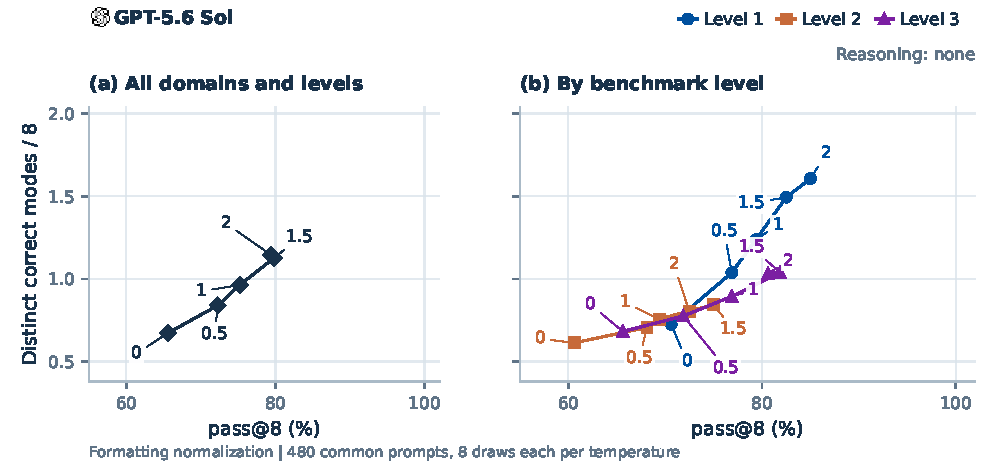
\includegraphics[width=.98\linewidth]{figures/gpt56_temperature_curve.pdf}
  \caption{\textbf{Nonzero temperatures yield greater observed eight-draw coverage.}
  GPT-5.6 Sol with reasoning \texttt{none}, typography normalization, and the same
  480 prompts at each of five temperatures (32 per domain--level cell, eight
  responses each). Left: an equal mean over all 15 domain--level cells; right:
  equal means over five domains at each level, identified by color and marker.
  The horizontal axis is empirical \texttt{pass@8}; the vertical axis averages
  distinct correct solution modes per eight responses, including unsolved prompts
  as zero. Labels give requested temperatures; segments connect measured point
  estimates in temperature order. Table~\ref{tab:gpt56-temperature} gives
  95\% whole-prompt bootstrap intervals. Mode counts depend on
  success and correct-answer variation and need not track \texttt{pass@8}.}
  \label{fig:gpt56-temperature-curve}
\end{figure}
}

\input{results/frontier_comparison_20260911_appendix.tex}

\input{results/hosted_level_averages_20260911.tex}

\begin{figure}[!htbp]
  \centering
  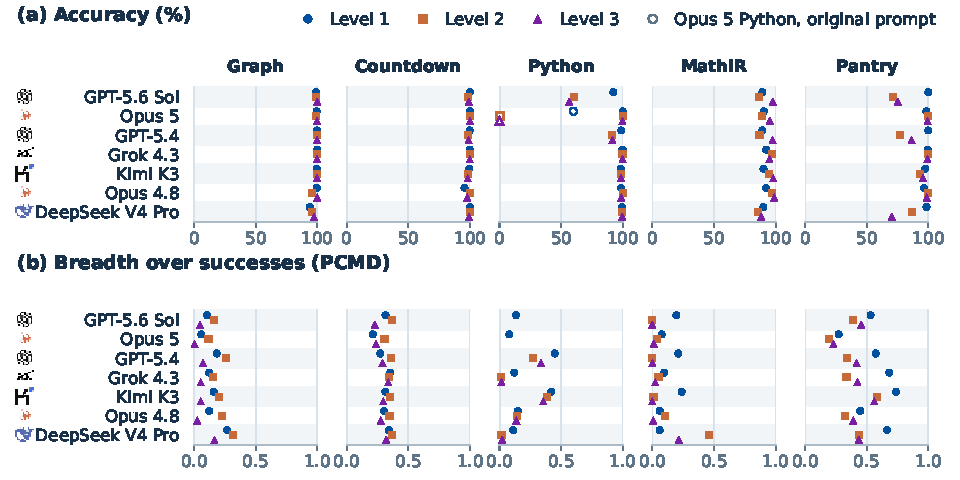
\includegraphics[width=\linewidth]{figures/hosted_verified_breadth.pdf}
  \caption{\textbf{Accurate hosted responses can still concentrate on few solution modes.}
  Columns show domains; colors and marker shapes distinguish Levels~1--3.
  Each deployment--domain--level cell uses 128 prompts and eight responses
  per prompt. Top: formatting-normalized response accuracy. Solid Opus~5
  \texttt{Python} marks use revised task wording without a system message; hollow marks
  show original wording. Bottom: promptwise \pmd{} under strict grading
  and original wording for every deployment, averaging over prompts with
  at least two verified draws. Cells with fewer than thirty eligible prompts
  are omitted. Thus the two rows use different grading and, for Opus~5
  \texttt{Python}, different prompt conditions. All marks are point estimates.
  Table~\ref{tab:hosted-level-averages-medium} gives per-level means;
  Table~\ref{tab:hosted-level-averages-parity} gives normalized success and
  mode counts on the four domains with common wording.}
  \label{fig:hosted-verified-breadth}
\end{figure}

\input{results/hosted_level_averages_20260911_parity.tex}

\input{results/gpt56sol_python_parity_20260918.tex}

\input{results/hosted_reasoning_off_20260912_main.tex}

\input{results/hosted_reasoning_off_20260912_appendix.tex}

\clearpage
\phantomsection
\begin{center}\large\textbf{Part VI. Idealized analysis}\end{center}
\addcontentsline{toc}{part}{Part VI. Idealized analysis}

\section{Mode Collapse and Verified Replay}
\label{app:theory}

This part collects the idealized analysis behind
Section~\ref{sec:collapse-mechanism}. The winner-take-all limit of
binary-reward policy gradient among equally rewarded outcomes is established
by \citet{sinha2026expected} and \citet{lochab2026ucpo} and is a replicator
system in the sense of \citet{hofbauer1998evolutionary}; we restate it in our
categorical model so that the later statements share its notation, and we do
not reprove it. What this part adds is: an exact identity showing that every
outcome-binary advantage induces the same conditional trajectory, so the
choice among Dr.GRPO, GRPO, and MaxRL rescales time without changing which
mode survives; a starvation bound showing that fresh groups supply no gradient
to a rare mode as its probability vanishes, whereas a fixed verified buffer
does; a uniform-in-time probability floor for every buffered mode under a
fixed replay dose, with the coupon-collection ordering that makes uniform
allocation optimal for finite-budget coverage; and the stationary target of a
reference-KL anchor, whose conditional allocation is the reference's. Every
statement is for one isolated prompt with independent categorical logits and
Euclidean expected-gradient flow. These results do not certify the
implemented AdamW/PPO trajectories. The final subsection states where the
assumptions stop and which signs and orderings the runs were checked against.
Table~\ref{tab:notation} defines the notation.

\subsection{Categorical model, and the known winner-take-all limit}
\label{app:theory-grpo-mean}
\label{app:theory-collapse}
\label{app:theory-objective-inertness}

The categorical model assigns one independent logit to each outcome
category. Its Euclidean mean flow and the subsequent finite-step, sampled,
and neural updates have different assumptions; a neural solution mode need
not have an independently optimized logit.

\begin{assumption}[Categorical mean-flow model]
\label{ass:categorical-mean-flow}
Fix one isolated prompt and a finite category set
$\mathcal A=\mathcal C\mathbin{\dot\cup}\mathcal N$ with $m\ge2$ correct
solution modes and $n\ge1$ incorrect categories, and set
$p_a=\operatorname{softmax}(z)_a$, $P=\sum_{c\in\mathcal C}p_c$, and
$q_c=p_c/P$, so that $P$ measures correctness while $q$ describes how that
correct probability is allocated among the individual correct modes.
\begin{enumerate}
\item[(A1)] \emph{Independent logits.} The policy carries one independently
  optimized logit for every category in $\mathcal A$, including one separate
  logit for each canonical correct mode.
\item[(A2)] \emph{Common length normalization.} Every response uses the same
  fixed length-normalization factor, absorbed into the positive coefficient
  of the group estimator.
\item[(A3)] \emph{Euclidean mean flow.} Updates are the infinitesimal expected
  updates in these logits, taken without optimizer preconditioning and without
  momentum carried between steps.
\item[(A4)] \emph{No competing regularizer.} Explicit reference KL is zero and
  no entropy term is present.
\item[(A5)] \emph{Nondegenerate start.} Logits are finite initially,
  $0<P(0)<1$, and the group size is $G\ge2$.
\end{enumerate}
\end{assumption}

Assumption~\ref{ass:categorical-mean-flow} comprises conditions (A1)--(A5).
AdamW's preconditioning and momentum violate (A3); finite, repeated PPO
updates are outside its infinitesimal on-policy limit. Response-specific
length normalization violates (A2), while reference KL and entropy
regularization violate (A4).

A language model induces probabilities over canonical outcomes, but those
probabilities alone do not determine its update geometry. Aggregating several
response strings into a mode does not generally commute with gradient flow
in response logits. The independent-category model therefore requires an
additional assumption beyond a neural policy and its validator equivalence
classes.

Draw a group $Z_1,\ldots,Z_G\stackrel{\mathrm{iid}}{\sim}p$ with $G\ge2$,
write $R_i=\1[Z_i\in\mathcal C]$, and let $R=\sum_iR_i$. At the on-policy
point where the PPO ratio equals one, consider the common-length estimator
\begin{equation}
  \widehat g_G
  =\frac1G\sum_{i=1}^G
   w(R)\left(R_i-\frac{R}{G}\right)\nabla_z\log p_{Z_i}.
  \label{eq:group-estimator}
\end{equation}
For the Dr.GRPO abstraction \citep{liu2025understanding}, $w(R)=1$ after
absorbing the fixed positive length-normalization factor. Reward-standardized
GRPO \citep{shao2024deepseekmath} with fixed common response-length
normalization takes $w(R)$ to be the reciprocal group reward standard
deviation on mixed groups (with a fixed numerical stabilizer if used).
Standard variable-length GRPO also weights each response by its own inverse
length; that response-specific factor cannot generally be absorbed into
$w(R)$ and is outside this equivalence.
In both cases, $0<w(\ell)<\infty$ for
$\ell\in\{1,\ldots,G-1\}$. The entire update is zero on all-equal
groups, without evaluating an undefined reciprocal standard deviation;
likewise, $w(R)R(G-R)$ below is defined as zero when $R=0$ or $R=G$. All
advantages and normalization weights are detached in the score estimator.

\begin{lemma}[A group baseline does not remove frequency amplification]
\enforcehalffinalproseline
\label{lem:grpo-mean}
For $0<P<1$, the expected update in Equation~\eqref{eq:group-estimator} is
\begin{equation}
  \E[\widehat g_G]
  =c_G(P)\nabla_z P,
  \qquad
  c_G(P)=
  \frac{\E\!\big[w(R)R(G-R)\big]}{G^2P(1-P)}>0.
  \label{eq:expected-group-gradient}
\end{equation}
For the Dr.GRPO abstraction, $c_G(P)=(G-1)/G$. Group centering and reward
standardization rescale the expected gradient without changing its direction
under these assumptions.
\end{lemma}

\begin{proof}
\enforcehalffinalproseline
Condition on the complete binary reward vector, whose sum is $R$. The score
identities give
\[
  \E[\nabla_z\log p_{Z_i}\mid R_i=1]=\nabla_z\log P,
  \qquad
  \E[\nabla_z\log p_{Z_i}\mid R_i=0]
  =\nabla_z\log(1-P).
\]
There are $R$ correct rows with centered reward $(G-R)/G$ and $G-R$
incorrect rows with centered reward $-R/G$. Therefore the conditional
expectation of the unaveraged sum in~\eqref{eq:group-estimator} is
\[
  w(R)\frac{R(G-R)}{G}
  \left(\nabla_z\log P-\nabla_z\log(1-P)\right)
  =w(R)\frac{R(G-R)}{GP(1-P)}\nabla_zP.
\]
The outer factor $1/G$ and expectation over
$R\sim\operatorname{Binomial}(G,P)$ yield~\eqref{eq:expected-group-gradient}.
For $w\equiv1$,
$\E[R(G-R)]=G(G-1)P(1-P)$, proving the Dr.GRPO value.
\end{proof}

The binomial identity also gives the denominator-free expression
\[
 c_G(P)=\frac{G-1}{G}\sum_{j=0}^{G-2}\binom{G-2}{j}
 w(j+1)P^j(1-P)^{G-2-j}.
\]
The binomial weights sum to one, so $c_G$ lies between
$(G-1)\min_j w(j+1)/G$ and $(G-1)\max_j w(j+1)/G$.
Thus $c_G$ extends smoothly and positively to $P=0,1$.

The practical MaxRL estimator has the same mean-gradient direction
\citep[Section~4.3 and App.~D, Theorem~5]{tajwar2026maxrl}. Its all-failure
convention determines the finite-group coefficient.

\begin{lemma}[Binary MaxRL has the same correctness-gradient direction]
\enforcehalffinalproseline
\label{lem:maxrl-mean}
Under Assumption~\ref{ass:categorical-mean-flow}, let MaxRL assign
$A_i^{\mathrm{MaxRL}}=GR_i/R-1$ when $R>0$ and zero when $R=0$, as in
Section~\ref{app:binary-maxrl}. For
$\widehat g_G^{\mathrm{MaxRL}}=G^{-1}\sum_i
 A_i^{\mathrm{MaxRL}}\nabla_z\log p_{Z_i}$ at the on-policy point, the
expected update is
\begin{equation}
  \E[\widehat g_G^{\mathrm{MaxRL}}]
  =c_G^{\mathrm{MaxRL}}(P)\nabla_zP,
  \qquad
  c_G^{\mathrm{MaxRL}}(P)
  =\frac{1-(1-P)^{G-1}}{P}>0,
  \label{eq:maxrl-expected-gradient}
\end{equation}
with continuous endpoint values
$c_G^{\mathrm{MaxRL}}(0)=G-1$ and
$c_G^{\mathrm{MaxRL}}(1)=1$.
\end{lemma}

\begin{proof}
\enforcehalffinalproseline
With $N=G$ and pass rate $P$, the estimator in
\citet[Theorem~5]{tajwar2026maxrl} equals
$\widehat g_G^{\mathrm{MaxRL}}$. Its expected coefficient is
$\sum_{j=0}^{G-2}(1-P)^j$, whose geometric sum gives
Equation~\eqref{eq:maxrl-expected-gradient} and its endpoint values.
The identity requires on-policy independent draws and the score identity.
\end{proof}

Integrating this coefficient gives the potential
\begin{equation}
 \Psi_{\mathrm{MaxRL}}(P)
 :=\int_0^P c_G^{\mathrm{MaxRL}}(s)\,ds
 =\sum_{k=1}^{G-1}\frac{1-(1-P)^k}{k}.
 \label{eq:maxrl-potential-finite-sum}
\end{equation}
In particular, $\Psi_{\mathrm{MaxRL}}(1)=\sum_{k=1}^{G-1}1/k$.
For binary rewards, best@\(k\) equals pass@\(k\), so this is a harmonic
mixture of sampling objectives for $k=1,\ldots,G-1$. The upper limit is
$G-1$ because the implemented centered estimator sets the entire update
to zero on all-failure groups. Subtracting an unconditional score baseline
even on those groups instead gives the order-$G$ estimator. These are exact
finite-group expectations at the on-policy point; subsequent clipping and
adaptive optimization can alter the expected update.

\paragraph{Winner-take-all collapse.}
Consider $\dot z=c_G(P)\nabla_zP$, with any of the smooth positive
coefficients established above: Dr.GRPO, common-length reward-standardized
GRPO, or the specified centered binary MaxRL estimator. This infinitesimal
expected-update model has
no sampling noise and uses independently optimized Euclidean logits. The
conditional dynamics follow the frequency-dependent replicator system
with fitness $f_c(q)=q_c$
\citep{hofbauer1998evolutionary,harper2009informationgeometry}.
The limit below is the outcome-level collapse of
\citet[Theorem~3.1]{sinha2026expected} for softmax outcome logits, and the
indifference-plus-amplification mechanism of
\citet[Sections~4.1--4.2]{lochab2026ucpo}. We restate it in the present
notation and give only the reduction to the replicator flow, which is the
step the replay results reuse; it is not a new result.

\begin{proposition}[Winner-take-all collapse in the categorical mean flow]
\enforcehalffinalproseline
\label{thm:grpo-collapse}
Under Assumption~\ref{ass:categorical-mean-flow}, if the conditional correct-mode
distribution $q(0)$ has a unique largest coordinate $c^\star$, then
\[
  P(t)\longrightarrow1,
  \qquad
  q_{c^\star}(t)\longrightarrow1,
  \qquad
  q_c(t)\longrightarrow0\quad(c\ne c^\star).
\]
Thus these categorical mean flows converge to a single correct solution
mode for generic initial conditions, even though every mode in $\mathcal C$
has exactly the same reward.
\end{proposition}

\begin{proof}
\enforcehalffinalproseline
Since $\dot P=c_G(P)\lVert\nabla_zP\rVert_2^2$ with
$\lVert\nabla_zP\rVert_2^2\ge P^2(1-P)^2(1/m+1/n)$ and $c_G$ positive and
continuous on $[0,1]$, $P$ cannot converge to an interior value, so
$P\to1$. Define the effective time
$\tau(t)=\int_0^t c_G(P(s))P(s)(1-P(s))\,ds$. Every logit has absolute
velocity at most $\dot\tau$, so $\tau(\infty)<\infty$ would give every logit
finite total variation and a finite limit, contradicting $P\to1$; hence
$\tau\to\infty$. On the correct simplex the change of time gives
\begin{equation}
  \frac{dq_c}{d\tau}
  =q_c\left(q_c-\sum_{d\in\mathcal C}q_d^2\right),
  \qquad
  \frac{d}{d\tau}\log\frac{q_c}{q_d}=q_c-q_d,
  \label{eq:grpo-replicator}
\end{equation}
the replicator flow with fitness $f_c(q)=q_c$
\citep{hofbauer1998evolutionary}, which is the log-ratio dynamics of
\citet[Theorem~3.1]{sinha2026expected}. For $c\ne c^\star$ the ratio
$\xi_c=q_c/q_{c^\star}$ satisfies
$d\log\xi_c/d\tau=-q_{c^\star}(1-\xi_c)\le-(1-\xi_c(0))/m$, so every
competitor vanishes relative to the initial leader over infinite effective
time, and normalization gives $q_{c^\star}\to1$.
\end{proof}

If several modes tie for the largest initial probability, symmetry preserves
the tie; the same ratio argument eliminates strictly smaller coordinates and
leaves the tied maxima uniform. An exactly uniform correct distribution is
therefore a special initial condition. The theorem concerns limiting
concentration: finite softmax logits already give positive probabilities at
every finite time, so finite-time positivity alone is not a retention result.

\begin{remark}
Proposition~\ref{thm:grpo-collapse} is asymptotic and requires (A1)--(A5).
Finite-time support loss and convergence of the stochastic neural optimizers
used in the experiments are outside its scope.
\end{remark}

\paragraph{Every outcome-binary advantage follows the same conditional trajectory.}
Expected binary reward is the total correct mass and is indifferent to its
allocation among correct modes \citep[Section~4.1]{lochab2026ucpo}. The
following identity is the finite-group form used below: the choice among
Dr.GRPO, reward-standardized GRPO, a leave-one-out baseline, and centered
MaxRL rescales optimization time along the correctness axis without changing
the trajectory of $q$ or the identity of the surviving mode.

\begin{lemma}[Conditional inertness of outcome-binary objectives]
\label{thm:objective-inertness}
Under Assumption~\ref{ass:categorical-mean-flow}, let $a(\cdot,\cdot)$ be any
detached advantage measurable with respect to the group's binary reward
vector, applied as
$\widehat g_a=G^{-1}\sum_{i}a(R_i,R)\nabla_z\log p_{Z_i}$ at the on-policy
point. Then
\begin{equation}
  \E[\widehat g_a]=c_a(P)\,\nabla_zP,
  \qquad
  c_a(P)=\frac1G\left(
  \frac{\E[R\,a(1,R)]}{P}-\frac{\E[(G-R)\,a(0,R)]}{1-P}\right).
  \label{eq:objective-inertness}
\end{equation}
If $c_a>0$ on $(0,1)$, then under the time change
$d\tau=c_a(P)P(1-P)\,dt$ the conditional distribution $q$ obeys
Equation~\eqref{eq:grpo-replicator} exactly, for every such $a$. Dr.GRPO,
reward-standardized GRPO, a leave-one-out baseline, the centered binary MaxRL
estimator, and any reweighting shaped by a pass@$k$ target are points in this
class. The choice among them rescales optimization time along the correctness
axis and leaves both the trajectory in $q$ and the identity of the surviving
mode unchanged.
\end{lemma}

\begin{proof}
\enforcehalffinalproseline
The score identities used in Lemma~\ref{lem:grpo-mean} give
$\E[\nabla_z\log p_{Z_i}\mid R_i=1]=\nabla_z\log P$ and
$\E[\nabla_z\log p_{Z_i}\mid R_i=0]=\nabla_z\log(1-P)$.
Independence of the draws means that conditioning also on the other rows'
rewards does not change either conditional mean. Since $a(R_i,R)$ depends
only on the binary rewards, conditioning on their complete vector and
summing the $R$ successful and $G-R$ failed rows gives
\[
  \E[\widehat g_a]
  =\frac1G\Big(\E[R\,a(1,R)]\nabla_z\log P
   +\E[(G-R)\,a(0,R)]\nabla_z\log(1-P)\Big).
\]
Substituting $\nabla_z\log P=\nabla_zP/P$ and
$\nabla_z\log(1-P)=-\nabla_zP/(1-P)$ yields
Equation~\eqref{eq:objective-inertness}. Hence
$\frac{d}{dt}\log(q_c/q_d)=\dot z_c-\dot z_d=c_a(P)P(1-P)(q_c-q_d)$.
For $c_a>0$, the positive time change $d\tau=c_a(P)P(1-P)\,dt$ gives
the replicator dynamics in Equation~\eqref{eq:grpo-replicator}.
\end{proof}

For a fixed reward-dependent advantage, the binomial identities
$R\binom GR=G\binom{G-1}{R-1}$ and
$(G-R)\binom GR=G\binom{G-1}{R}$ give
\begin{equation}
 c_a(P)=\sum_{j=0}^{G-1}\binom{G-1}{j}P^j(1-P)^{G-1-j}
 \big[a(1,j+1)-a(0,j)\big],
 \label{eq:inertness-polynomial}
\end{equation}
a polynomial in $P$ of degree at most $G-1$. Finite advantage values
therefore give a smooth, bounded coefficient on $[0,1]$. This bounded coefficient is what the retention argument in
App.~\ref{app:theory-replay} uses.

\begin{corollary}[MaxRL amplification of the correctness gradient]
\enforcehalffinalproseline
\label{cor:maxrl-starvation}
For the coefficients of Lemmas~\ref{lem:grpo-mean} and~\ref{lem:maxrl-mean},
\[
 \frac{c_G^{\mathrm{MaxRL}}(P)}{c_G^{\mathrm{Dr.GRPO}}}
 =\frac{G\big[1-(1-P)^{G-1}\big]}{(G-1)P}.
\]
This ratio is nonincreasing in $P$, with limits $G$ as $P\to0$ and
$G/(G-1)$ as $P\to1$. It is strictly decreasing for $G>2$ and constant
at $2$ for $G=2$. At the same policy, MaxRL therefore multiplies the
Dr.GRPO correctness-gradient coefficient by a factor approaching $G$ when
correctness is small. The probability of a nonzero fresh task component
remains bounded by the mixed-group probability in
Lemma~\ref{lem:replay-gradient-availability} for both estimators.
\end{corollary}

\begin{proof}
\enforcehalffinalproseline
Divide $c_G^{\mathrm{MaxRL}}(P)=[1-(1-P)^{G-1}]/P$ by $(G-1)/G$.
The finite-series identity
$c_G^{\mathrm{MaxRL}}(P)=\sum_{j=0}^{G-2}(1-P)^j$
gives the endpoint limits and monotonicity. For $G=2$ the sum is the
constant $1$; for $G>2$ it contains the strictly decreasing term $1-P$.
\end{proof}

\subsection{A replay signal when fresh groups supply none}
\label{app:theory-gradient-availability}

\begin{lemma}[Fresh-group starvation]
\enforcehalffinalproseline
\label{lem:replay-gradient-availability}
Under Assumption~\ref{ass:categorical-mean-flow} with correctness probability
$P$, draw $G$ fresh categories independently. The probability of a
mixed-reward group is
\[
 h_G(P)=1-P^G-(1-P)^G\le G\min\{P,1-P\}.
\]
Every all-equal group has zero fresh task component for
Equation~\eqref{eq:group-estimator} and for the specified centered MaxRL
estimator, so the probability of a nonzero fresh task component is at most $h_G(P)$.
\end{lemma}

\begin{proof}
\enforcehalffinalproseline
The all-correct and all-incorrect events are disjoint and have probabilities
$P^G$ and $(1-P)^G$. A mixed group needs at least one correct and at least
one incorrect sample, so a union bound over the $G$ draws gives both
$h_G(P)\le GP$ and $h_G(P)\le G(1-P)$, and hence the stated minimum.
\end{proof}

\begin{lemma}[Replay ascent persists as fresh signal vanishes]
\enforcehalffinalproseline
\label{lem:replay-ascent}
Under Assumption~\ref{ass:categorical-mean-flow}, let
$\mathcal B\subseteq\mathcal C$ be a nonempty fixed verified buffer with
normalized positive weights $w_b$, let $R_w=-\sum_b w_b\log p_b$ with replay
coefficient $\rho_w>0$, and extend $w$ by zero outside the buffer to obtain $\bar w$. The
deterministic replay ascent vector is
\[
 v^{\rm replay}=-\rho_w\nabla R_w=\rho_w(\bar w-p),
\]
which vanishes only at $p=\bar w$. If $p_b\le w_b/2$ for a buffered mode, then
$v^{\rm replay}_b\ge\rho_w w_b/2$, even when $b$ is absent from the fresh
group. For a uniform buffer of $k\ge2$ modes and fixed $\rho_w>0$, as
$p\to\mathbf e_b$ at one buffered correct mode, $h_G(P)\to0$ whereas
$\|v^{\rm replay}\|_2\to\rho_w\sqrt{1-1/k}>0$.
\end{lemma}

\begin{proof}
\enforcehalffinalproseline
For $R_w=-\sum_b w_b\log p_b$, the softmax score identity gives
$\partial R_w/\partial z_a=p_a-\bar w_a$, proving the replay formula and
coordinate bound. Finally,
\[
 \|\bar w-\mathbf e_b\|_2^2=(1-1/k)^2+(k-1)/k^2=1-1/k,
\]
which gives the strictly positive limiting norm for $k\ge2$.
\end{proof}

\begin{remark}
A fixed verified buffer can supply a replay signal when the fresh task
gradient is unavailable. Lemma~\ref{lem:replay-gradient-availability}
bounds the probability of a nonzero fresh task component; it does not bound
its magnitude or account for other loss terms, clipping, or momentum. The vector in
Lemma~\ref{lem:replay-ascent} averages the fixed buffer, so a stochastic
exemplar draw realizes it only in expectation, and a nonzero logit coordinate
can still be annihilated by a degenerate neural Jacobian. Replay also need not
increase the next mixed-group probability, since $h_G(P)$ is largest at
$P=1/2$.
\end{remark}

With uniformly bounded detached advantages, the expected sampled-logit
update vanishes as the category probability tends to zero, even when
advantages depend on the group. Exact entropy gradients have unbounded
surprisal weights and therefore require a separate boundary analysis.

\begin{lemma}[Bounded sampled scores have no probability-independent boundary force]
\enforcehalffinalproseline
\label{lem:sampled-score-bound}
Under Assumption~\ref{ass:categorical-mean-flow}, condition on the training history, draw
$Z_1,\ldots,Z_G$ independently from $p$, and let $a_i$ be any detached,
possibly group-dependent advantages with $|a_i|\le B$. To interpret the
bound uniformly as $p_b\to0$, assume a finite $B$ independent of that limit.
At the on-policy point define
\[
 \widehat g=\frac1G\sum_{i=1}^G a_i(\mathbf e_{Z_i}-p).
\]
For every category $b$,
\[
 |\E[\widehat g_b]|\le\E|\widehat g_b|
 \le 2B p_b(1-p_b).
\]
On a group with no draw of $b$, exactly
$\widehat g_b=-p_bG^{-1}\sum_i a_i$; it is zero if the applied advantages
sum to zero. By comparison, the verified-replay component for a fixed target
$w$ has logit velocity $\rho(w_b-p_b)$, which approaches $\rho w_b>0$
for a buffered category as $p_b\to0$.
\end{lemma}

\begin{proof}
\enforcehalffinalproseline
Use the triangle inequality and $|a_i|\le B$. Each marginal draw satisfies
$\E|\1\{Z_i=b\}-p_b|=2p_b(1-p_b)$, irrespective of the dependence of
$a_i$ on the group. On the absence event all indicator terms are zero.
The replay formula follows by differentiating $-\sum_b w_b\log p_b$.
\end{proof}

The bound compares the isolated logit-gradient components. It does not prove
inevitable collapse, rule out retention by a bounded estimator, or guarantee
that replay dominates the full update. An unsampled mode can still change
through softmax normalization or shared parameters. Exact entropy is outside
the uniformly bounded-score premise because its surprisal is unbounded near
zero; the lemma is not an impossibility result for entropy regularization.
Nor does the absence of a mode from a finite sample establish zero probability.

\subsection{Fixed-buffer replay and retention}
\label{app:theory-replay}

Let $\mathcal B\subseteq\mathcal C$ be a nonempty fixed buffer of $k$ modes that
the policy has produced and the validator has accepted. Uniform verified replay
uses one exemplar per buffered mode and, in the categorical reduction, minimizes
\begin{equation}
  R_{\mathcal B}(z)
  =-\frac1k\sum_{b\in\mathcal B}\log p_b.
  \label{eq:verified-replay-loss}
\end{equation}
For the uniform buffer target $w$, the likelihood-replay objective is
$R_{\mathcal B}=H(w)+\mathrm{KL}(w\|p)$
\citep[App.~D.1, v4]{li2025divergence}. The target assigns mass
$1/k$ to each buffered mode and zero elsewhere. Decreasing this loss can raise
total buffer mass as well as redistribute mass within the buffer; the buffer is
not the conditioning event for $p$.

In an averaged continuous-time model, absorb a fixed round-robin replay
frequency and loss scale into an effective dose $\rho>0$. This assumes a
fixed eligible-buffer set and constant relative weighting; it does not identify
finite alternating updates with simultaneous gradient flow. For one
isolated prompt, the categorical mean flow for any of the three fresh
binary-reward estimators with verified replay is
\begin{equation}
  \dot z
  =c_G(P)\nabla_zP-\rho\nabla_zR_{\mathcal B}(z).
  \label{eq:replay-mean-flow}
\end{equation}
Let $\Psi(P)=\int_0^P c_G(s)\,ds$. For the finite-group estimators in Lemmas~\ref{lem:grpo-mean}
and~\ref{lem:maxrl-mean}, $c_G$ has a finite positive extension to $[0,1]$;
in particular, Dr.GRPO has $c_G=(G-1)/G$ and MaxRL has
$c_G=[1-(1-P)^{G-1}]/P$. More generally, Lemma~\ref{thm:objective-inertness} and
Equation~\eqref{eq:inertness-polynomial} give
$c_a(P)\nabla_zP$ for every fixed, bounded reward-measurable advantage,
with $c_a$ a polynomial. Its integral $\Psi_a$ is also bounded on $[0,1]$,
so the retention argument applies even when the fresh coefficient changes
sign. Define
\begin{equation}
  F_{\mathcal B}(z)=\rho R_{\mathcal B}(z)-\Psi(P(z)).
  \label{eq:replay-potential}
\end{equation}
Then~\eqref{eq:replay-mean-flow} is exactly gradient flow
$\dot z=-\nabla_zF_{\mathcal B}$.

\begin{theorem}[Verified replay prevents buffered-mode extinction]
\enforcehalffinalproseline
\label{thm:replay-retention}
Under Assumption~\ref{ass:categorical-mean-flow}, suppose logits are finite
at time $T$ and thereafter the nonempty verified buffer $\mathcal B$ is fixed,
fits within replay capacity, and receives a
fixed positive effective replay dose $\rho$, the fresh objective being any
bounded reward-measurable one in the sense of
Lemma~\ref{thm:objective-inertness}. Set
$\Psi_{\max}=\max_{s\in[0,1]}\Psi(s)$, which is finite, and under
\eqref{eq:replay-mean-flow} define
\[
  C_T
  =R_{\mathcal B}(z(T))
   +\frac{\Psi_{\max}-\Psi(P(T))}{\rho}.
\]
Then for every $b\in\mathcal B$ and every $t\ge T$,
\begin{equation}
  p_b(t)\ge \exp(-kC_T)>0.
  \label{eq:replay-retention-bound}
\end{equation}
Thus each buffered probability is uniformly bounded away from zero for all
$t\ge T$, including asymptotically, even when the buffer does not cover every
correct mode. This is stronger than finite-time positivity, which already
follows from finite softmax logits without replay.
\end{theorem}

\begin{proof}
\enforcehalffinalproseline
The smooth vector field has bounded velocity because $c_G$,
$\nabla_zP$, and $\nabla_zR_{\mathcal B}$ are bounded, so finite initial
logits give a flow for every finite $t\ge T$. Along this flow,
\[
  \frac{d}{dt}F_{\mathcal B}(z(t))
  =-\lVert\nabla_zF_{\mathcal B}(z(t))\rVert_2^2\le0.
\]
Since $\Psi(P(t))\le\Psi_{\max}$,
\[
  R_{\mathcal B}(z(t))
  \le R_{\mathcal B}(z(T))
     +\frac{\Psi_{\max}-\Psi(P(T))}{\rho}
  =C_T.
\]
Every $-\log p_b$ is nonnegative and their sum is
$kR_{\mathcal B}$. Therefore
$-\log p_b(t)\le kC_T$ for every buffered mode, which is exactly
Equation~\eqref{eq:replay-retention-bound} for every time after $T$.
\end{proof}

For the nonnegative coefficients of the named fresh estimators,
$\Psi_{\max}=\Psi(1)$, recovering the simpler constant. Signed coefficients
also satisfy the retention bound, but need not yield $P\to1$.
The elementary floor is qualitative and can be numerically vacuous. For example, at
$k=16$ even a hypothetical $C_T=160$ gives $e^{-2560}$, far below any useful
evaluation probability. The argument establishes a uniform-in-time lower
bound in the stated ideal flow, not practical visibility or a prediction for
the experimental replay loss. The effective dose also depends on relative
fresh/replay frequencies, not the replay coefficient alone.

A common nonnegative, locally integrable rate $\eta(t)$ multiplying both
terms of~\eqref{eq:replay-mean-flow} preserves the energy bound, since
$\dot F_{\mathcal B}=-\eta(t)\|\nabla F_{\mathcal B}\|_2^2\le0$.
The convergence statements below additionally require
$\int_T^\infty\eta(t)\,dt=\infty$ and then follow by reparameterizing
optimization time. Infinitely many replay visits alone establish neither
this condition nor a fixed replay-to-fresh weighting. Different time-varying
relative weights are outside the fixed-potential argument.

\paragraph{Full coverage and the categorical target.}
\begin{corollary}[Conditional full-coverage categorical limit]
\enforcehalffinalproseline
\label{cor:replay-no-collapse}
Assume the conditions of Theorem~\ref{thm:replay-retention} and that by time
$T$ the buffer covers the full correct support, $\mathcal B=\mathcal C$.
Assume additionally $c_G(P)\ge0$ on $[0,1]$, as for the three named
estimators. Let
$u_c=1/m$ on $\mathcal C$. Then the categorical mean flow converges to
\[
  P(t)\longrightarrow1,
  \qquad q(t)\longrightarrow u.
\]
Consequently
\[
  \min_{c\in\mathcal C}q_c(t)\longrightarrow\frac1m,
  \qquad
  \mathcal H(q(t))\longrightarrow\log m,
\]
so asymptotic concentration onto a strict subset of the correct modes is
impossible under full coverage. \pmd{} may nevertheless decline transiently
before converging to its uniform maximum.
\end{corollary}

\begin{proof}
\enforcehalffinalproseline
For full coverage,
\begin{equation}
 R_{\mathcal C}=\log m-\log P+\mathrm{KL}(u\|q).
 \label{eq:replay-mass-uniformity-decomposition}
\end{equation}
The potential is bounded below by $-\Psi_{\max}$, so its descent gives
$\int_T^\infty\|\nabla F_{\mathcal C}\|_2^2dt<\infty$. The fixed reward-measurable
advantage gives a smooth $c_G$ on $[0,1]$, and softmax derivatives and the cross-entropy
gradient are bounded. Thus the Hessian of $F_{\mathcal C}$ and the velocity
are bounded; the gradient along the trajectory is uniformly continuous.
Square integrability then implies $\nabla F_{\mathcal C}\to0$: recurring
gradients of fixed positive size would otherwise contribute energy over
intervals of a uniform minimum length.

Every limiting probability vector therefore satisfies the correct-coordinate
equations
\[
 0=\rho(p_c-1/m)-c_G(P)p_c(1-P).
\]
Summing them gives $0=-(1-P)(\rho+c_G(P)P)$, hence $P=1$. Each correct
coordinate is then $1/m$ and every incorrect coordinate is zero. Compactness
of the probability simplex and uniqueness of this limit establish convergence
of the probability vector.
\end{proof}

\begin{corollary}[Uniform allocation maximizes finite-budget coverage]
\enforcehalffinalproseline
\label{cor:coupon-uniform-coverage}
Fix correctness $P\in(0,1]$ and $m\ge2$ possible correct keys.
Let $D_K(P,q)$ count distinct verified keys in $K$ independent draws with
key probabilities $Pq_1,\ldots,Pq_m$ and failure probability $1-P$.
For $u=(1/m,\ldots,1/m)$, every $K\ge1$ and $r=1,\ldots,m$ satisfy
\begin{equation}
 \Pr[D_K(P,u)\ge r]\ge\Pr[D_K(P,q)\ge r].
 \label{eq:coupon-uniform-coverage}
\end{equation}
Thus uniform conditional allocation maximizes expected \texttt{distinct@}$K$
at fixed correctness, as well as every coverage tail probability. This is
the coupon-collection ordering of
\citet[Theorem~3, v1]{anceaume2015coupon}, applied to independent draws
from a fixed policy over a finite catalogue of verified execution keys.
\end{corollary}
\begin{proof}
\enforcehalffinalproseline
Map each correct key to a coupon of mass $Pq_c$ and every failure to the
null coupon of mass $1-P$. The cited theorem makes the time to collect $r$
distinct non-null coupons stochastically smallest when each has mass $P/m$.
The event that this time is at most $K$ is exactly $D_K\ge r$.
Zero coordinates and $P=1$ follow by continuity of finite-horizon
probabilities. Summing the tail inequalities over $r=1,\ldots,m$ gives the
same ordering of expected distinct counts for every finite sampling budget
at the same correctness level and over the same catalogue of possible keys.
\end{proof}
This sampling optimum does not assert that a training algorithm reaches the
uniform allocation.

\paragraph{Positive weights and the implemented length normalization.}
Uniformity of the target is separate from protection against extinction.
For fixed weights $w_b>0$ with $\sum_{b\in\mathcal B}w_b=1$, define
$R_w=-\sum_b w_b\log p_b$ and use replay coefficient $\rho_w>0$.
The same potential argument gives, for all $t\ge T$,
\[
 p_b(t)\ge\exp(-C_{T,w}/w_b),\qquad
 C_{T,w}=R_w(z(T))+\frac{\Psi_{\max}-\Psi(P(T))}{\rho_w}.
\]
For the following convergence statements assume $c_G\ge0$.
If $\mathcal B=\mathcal C$, then
$R_w=H(w)-\log P+\mathrm{KL}(w\|q)$, and the independent-logit limit is
$P\to1$, $q\to w$. The preceding stationarity proof applies with $1/m$
replaced by $w_c$: summing the correct-coordinate equations forces $P=1$,
then each equation forces $p_c=w_c$.

A partial buffer has a stronger limitation in this same ideal flow. For any
fixed nonempty $\mathcal B\subseteq\mathcal C$ and fixed positive weights
summing to one, extend $w$ by zero to $\bar w$ on all categories. Then
$p(t)\to\bar w$, so even correct modes outside the fixed buffer vanish
asymptotically. For $F=\rho_wR_w-\Psi(P)$, the preceding energy and
bounded-Hessian argument still gives $\nabla F\to0$; neither argument
requires full buffer coverage.
At every subsequential probability limit, the correct-coordinate equations are
\[
 0=\rho_w(p_c-\bar w_c)-c_G(P)p_c(1-P).
\]
Summing over correct categories gives
$0=-(1-P)(\rho_w+c_G(P)P)$, hence $P=1$; each equation then gives
$p_c=\bar w_c$, and all incorrect mass is zero. Compactness and uniqueness
of this limiting probability vector prove convergence. Thus protecting a
fixed set of buffered modes need not preserve unbuffered correct alternatives.
This conclusion concerns the fixed-buffer categorical flow, not changing-buffer
or stochastic neural training.

This distinction matters for the implemented mean-token exemplar loss.
Even if each key were represented by exactly one categorical exemplar of
fixed length $L_b$, its loss would be $A R_w$, where
\[
 A=\frac1k\sum_{b\in\mathcal B}\frac1{L_b},\qquad
 w_b=\frac{L_b^{-1}}{\sum_{j\in\mathcal B}L_j^{-1}}.
\]
Its effective categorical replay coefficient would be $\rho_w=\rho A$.
The full-coverage limit would therefore weight shorter exemplars more, and
would be uniform only for equal lengths. For an actual language model,
$\pi_\theta(e_b\mid x)$ is only one contribution to the total key probability.
Equal averaging of per-token exemplar scores does not imply uniform learned
key probabilities; the categorical uniformity corollary is not that claim.

Full support is an additional premise, not a consequence of replay. In
\texttt{Python} factors, evaluation prompts admit 16--1{,}512 correct execution
modes (mean 229.44), while the buffer capacity is 16. The
full-coverage corollary therefore cannot supply a domain-wide guarantee there. The retention theorem protects only
buffered modes; it supplies no probability floor for an unbuffered key.

\subsection{Reference-KL stationary targets}
\label{app:theory-kl}

Assumption~\ref{ass:categorical-mean-flow}(A4) sets the reference-KL
coefficient to zero, as in the default training setting of
Table~\ref{tab:run-contract}. A positive fixed-reference coefficient changes
the categorical target: for Dr.GRPO and centered MaxRL, the unique
full-support stationary policy allocates its correct mass in the same
proportions as the reference, so the anchor can retain only the diversity its
reference already carries. The measured comparison is in
App.~\ref{app:kl-measured}.

For this analysis, replace (A4) by

\begin{itemize}
\item[(A4$'$)] \emph{Reference KL.} A fixed reference $\mu$ with full support
  on the category set $\mathcal A$ enters with a positive coefficient $\beta$,
  and no entropy term is present alongside it.
\end{itemize}
The KL estimator in GRPO has expectation $\mathrm{KL}(p\,\|\,\mu)$
under samples drawn from $p$ \citep{shao2024deepseekmath}. Unbiasedness of
this value does not imply that differentiating it at fixed samples gives an
unbiased gradient of the distributional KL. With the KL differentiated
exactly, write $D(z)=\mathrm{KL}(p(z)\,\|\,\mu)$. The prompt-isolated
categorical mean flow is
\begin{equation}
  \dot z=c_G(P)\nabla_zP-\beta\nabla_zD(z),
  \qquad
  \nabla_{z_b}D=p_b\big(\log(p_b/\mu_b)-D\big),
  \label{eq:kl-mean-flow}
\end{equation}
which is the negative gradient flow of
$F_\beta(z)=-\Psi(P(z))+\beta D(z)$, with $\Psi'=c_G$ as in
Equation~\eqref{eq:replay-potential}.

\begin{lemma}[Reverse-KL sublevels and replay barriers]
\enforcehalffinalproseline
\label{lem:kl-no-barrier}
For a full-support reference,
$D=\mathrm{KL}(p\|\mu)\le\log(1/\min_a\mu_a)$ on the simplex, while
$R_{\mathcal B}\to\infty$ if a buffered coordinate vanishes. More precisely,
\[
 \inf_{p:p_b=0}D(p)=\log\frac1{1-\mu_b}.
\]
Thus every finite replay-loss sublevel bounds each protected probability
away from zero. A reverse-KL sublevel $\{D\le B\}$ does so for coordinate $b$
if $B<-\log(1-\mu_b)$, but includes a point with $p_b=0$ if
$B\ge-\log(1-\mu_b)$.
\end{lemma}
\begin{proof}
\enforcehalffinalproseline
The global bound follows from $\sum_ap_a\log p_a\le0$ and
$-\sum_ap_a\log\mu_a\le\log(1/\min_a\mu_a)$.
On the face $p_b=0$, write $\widetilde\mu_a=\mu_a/(1-\mu_b)$ for $a\ne b$.
Then $D(p)=\mathrm{KL}(p\|\widetilde\mu)-\log(1-\mu_b)$, whose minimum is
attained at $\widetilde\mu$. Continuity and compactness exclude that face
from any strictly lower sublevel and give a positive coordinate minimum.
For replay, $-\log p_b\le kR_{\mathcal B}$ gives the bound directly.
\end{proof}

Descent of $F_\beta$ gives
$D(p(t))\le [F_\beta(z(T))+\Psi_{\max}]/\beta$.
This energy bound excludes the face $p_b=0$ when its right side is below
$-\log(1-\mu_b)$; an arbitrary initial energy need not satisfy that condition.
A trajectory can have a positive probability floor even when this sublevel
bound does not establish one.

\begin{proposition}[The retained conditional is the reference's]
\enforcehalffinalproseline
\label{prop:kl-stationary}
Under Assumption~\ref{ass:categorical-mean-flow} with (A4$'$), using the
Dr.GRPO or centered MaxRL coefficient, the flow
\eqref{eq:kl-mean-flow} has exactly one stationary policy of full support,
\[
  p^\star_a\propto\mu_ae^{\lambda R_a},
  \qquad
  \lambda=c_G(P^\star)/\beta,
  \qquad
  R_a=\1[a\in\mathcal C],
\]
with $\lambda=(G-1)/(G\beta)$ in closed form for the Dr.GRPO coefficient, and
a unique $\lambda$ for the MaxRL coefficient. Consequently
\[
  q^\star=\mu|_{\mathcal C},
  \qquad
  \mathcal H(q^\star)=\mathcal H(\mu|_{\mathcal C}),
  \qquad
  \operatorname{logit}P^\star=\operatorname{logit}\mu(\mathcal C)+\lambda .
\]
This stationary conditional does not depend on $\beta$: the coefficient sets
the correctness level there and leaves the allocation among correct modes at
the reference's.
\end{proposition}

\begin{proof}
\enforcehalffinalproseline
Stationarity of~\eqref{eq:kl-mean-flow} in a coordinate with $p_b>0$ reads
$c_G(P)(R_b-P)=\beta(\log(p_b/\mu_b)-D)$, so
$\log(p_b/\mu_b)=D+(c_G(P)/\beta)(R_b-P)$ and the $b$-independent terms are
absorbed by normalization, giving the stated form with $\lambda=c_G(P)/\beta$.
Conversely each $\lambda\ge0$ determines
$P(\lambda)=\mu(\mathcal C)e^\lambda/(\mu(\mathcal C)e^\lambda+1-\mu(\mathcal C))$,
strictly increasing from $\mu(\mathcal C)$ to $1$. The consistency requirement
$\lambda=c_G(P(\lambda))/\beta$ has a solution by the intermediate value
theorem, since the left side increases from $0$ without bound while the right
side is positive and bounded; it is unique whenever $c_G$ is non-increasing,
which covers the constant Dr.GRPO coefficient and
$c_G^{\mathrm{MaxRL}}(P)=[1-(1-P)^{G-1}]/P$, nonincreasing from $G-1$
to $1$ and strictly decreasing for $G>2$.
Two correct modes give $\log(p_c/\mu_c)=\log(p_d/\mu_d)$, hence
$q^\star\propto\mu$ on $\mathcal C$, which is $\beta$-free. The logit identity
is $P^\star/(1-P^\star)=[\mu(\mathcal C)/(1-\mu(\mathcal C))]e^\lambda$.
\end{proof}

Dr.GRPO with exact reference KL is an entropy-regularized softmax bandit, so
\citet[Theorem~5 and Lemma~13]{mei2020softmaxpg} give convergence of exact
gradient steps to this stationary policy together with a positive
trajectory-wide probability floor; its Gibbs target is the regularized
maximizer of \citet[Proposition~1]{geist2019regmdp}. We do not restate those
results. The contrast with replay is the one in
Lemma~\ref{lem:sampled-score-bound}: by Equation~\eqref{eq:kl-mean-flow} the
reverse-KL restoring force on a depleted coordinate is proportional to $p_b$
and vanishes with it, whereas replay's force on a buffered coordinate has the
positive limit $\rho w_b$.

\subsection{Where the categorical guarantees stop, and what was measured}
\label{app:theory-evidence-map}
\label{app:theory-entropy}
\label{app:theory-entropy-comparison}
\label{app:theory-neural-replay-response}
\label{app:theory-measured-signatures}

\paragraph{Dependence on optimization geometry.}
For a smooth parameterization $z=z(\theta)$ with Jacobian
$J_\theta=\partial z/\partial\theta$, Euclidean parameter flow instead
induces $\dot z=c_G(P)J_\theta J_\theta^\top\nabla_zP$. Proposition~\ref{thm:grpo-collapse}
uses $J_\theta J_\theta^\top=I$ and does not automatically
extend to arbitrary shared parameters or another optimization metric. Equal
binary reward alone does not force this winner selection. The natural policy
gradient update of \citet[Lemma~15]{agarwal2021policygradient}, specialized to
this bandit, is $p_a^+\propto p_a\exp(\eta c_G(P)R_a)$ and preserves
every ratio of correct probabilities at each finite step. Its continuous
version has $\dot z_a=c_G(P)(R_a-P)$, with
$R_a=\1[a\in\mathcal C]$. The distinction between Euclidean and natural
updates also underlies the tabular entropy identities of
\citet[Theorems~1--2]{cui2025entropy}; entropy and verified-mode diversity
remain different observables.

\paragraph{Exact entropy is a different comparator.}
For a known full correct support and uniform $u$, the elementary identities
\[
 H(q)=\log m-\mathrm{KL}(q\|u),\qquad
 R_u(p)=\log m-\log P+\mathrm{KL}(u\|q)
\]
show that exact conditional entropy and categorical replay both favor a
uniform conditional target. With strictly increasing correctness potential
$\Psi$, both $\Psi(P)+\beta H(q)$ and $\Psi(P)-\rho R_u(p)$ have the unique
global optimum $P=1,q=u$ in probability space on the simplex with $P>0$,
for positive coefficients. This is a boundary limit for finite-logit softmax
policies. The optimum follows from nonnegativity of KL and increasing
$\Psi$; it does not assert convergence of either neural update. The KL direction distinguishes their
loss level sets \citep{pereyra2017confidencepenalty,agarwal2021policygradient}:
replay loss diverges when a protected coordinate vanishes, whereas
conditional entropy can remain $\log(m-1)$ with one missing mode.

Exact full-output entropy is a third objective and also regularizes incorrect
mass. Exact tabular entropy-regularized policy gradient has its own positive
probability and convergence guarantees under specified assumptions
\citep{mei2020softmaxpg}; Proposition~\ref{thm:grpo-collapse} contains no entropy term.
The sampled semantic scores in the experiments are not exact gradients of
full-output or conditional verified-key entropy. Neither their empirical
comparison nor the bounded-score lemma is an impossibility result for entropy.

\paragraph{Discovery and optimization remain separate requirements.}
Retention starts after a verified key enters active memory. Actual insertion
depends on generation, validation, capacity, and eligibility; a positive
sampling probability alone does not establish eventual admission. Once a
non-evicting capacity-16 buffer fills, an unbuffered key can remain ineligible.
Changing membership or exemplar weights changes the loss being bounded, so
fixed-buffer descent cannot simply be carried across those changes. In
particular, the fixed-weight argument does not cover a target whose weights
continue to change with fresh observation counts.

Extending the fixed-potential descent to a discrete, shared-parameter
optimizer would need an energy bound of the form
$F(\theta_{n+1})\le F(\theta_n)+\epsilon_n$ with summable $\epsilon_n$, and
neither a positive replay coefficient nor a small nominal learning rate
establishes one. Adam moments, clipping, momentum, prompt scheduling, and
buffer changes are not covered by the exact-flow proofs, and the experiments
do not establish the required energy control. The one neural statement made
here is local.

With shared parameters, a replay update's effect on a particular exemplar
depends on interference among score gradients and on the optimizer's
response. A lower bound on that exemplar's change in log probability can be
obtained from the realized parameter step, without assuming any global
potential descent.

\begin{proposition}[Local replay response under shared parameters]
\enforcehalffinalproseline
\label{prop:neural-replay-local-response}
For a fixed buffer of $k$ complete exemplars, define
\[
 \ell_b(\theta)=\frac{\log\pi_\theta(e_b\mid x_b)}{L_b},\qquad
 h_b=\nabla_\theta\ell_b(\theta),\qquad
 \bar h=\frac1k\sum_{j=1}^k h_j.
\]
Suppose a step has the form
$\Delta=\eta H(g+\lambda\bar h)+u$, where $\eta,\lambda\ge0$,
$H$ is a fixed symmetric positive semidefinite matrix for this step,
$g$ is the fresh ascent direction, and $u$ is the remaining update.
Assume $\ell_b$ is twice differentiable and its Hessian has operator norm
at most $B_b$ along $\{\theta+s\Delta:0\le s\le1\}$.
Set
\[
 K_{bj}=h_b^\top Hh_j,\qquad
 \kappa_b=\frac1k\sum_jK_{bj},\qquad
 m_b=\eta h_b^\top Hg+\eta\lambda\kappa_b
       +h_b^\top u-\frac{B_b}{2}\|\Delta\|_2^2.
\]
Then
\begin{equation}
 \ell_b(\theta+\Delta)-\ell_b(\theta)\ge m_b,
 \qquad
 \pi_{\theta+\Delta}(e_b\mid x_b)
    \ge\pi_\theta(e_b\mid x_b)e^{L_bm_b}.
 \label{eq:neural-replay-local-response}
\end{equation}
In particular, $m_b>0$ guarantees that this update increases the complete
exemplar's probability, whether or not it appeared among the fresh samples.
\end{proposition}

\begin{proof}
\enforcehalffinalproseline
Taylor's theorem with the Hessian bound gives
$\ell_b(\theta+\Delta)-\ell_b(\theta)
 \ge h_b^\top\Delta-(B_b/2)\|\Delta\|_2^2$.
Substitution of the stated step and
$h_b^\top H\bar h=k^{-1}\sum_jK_{bj}$ proves the first inequality.
Multiplication by $L_b$ and exponentiation prove the second.
\end{proof}

The required replay response is a row average $\kappa_b$ of the score Gram
matrix, not only its nonnegative diagonal entry $K_{bb}$. A sufficient
interference condition is $\kappa_b>0$, with replay strength satisfying
\[
 \eta\lambda\kappa_b>
   -\eta h_b^\top Hg-h_b^\top u
       +\frac{B_b}{2}\|\Delta\|_2^2.
\]
This inequality includes the step's curvature cost, which itself depends on
the chosen dose; arbitrarily increasing $\lambda$ is not a sufficient rule.

The interference condition cannot be dropped. For example, consider three
categorical logits sharing one scalar parameter, with slopes $(1,-2,0)$.
At a point with probabilities $(s,s,1-2s)$, where $0<s<1/4$, let the first
two categories be correct and buffered. Their unit-length log-score gradients
are $h_1=1+s$ and $h_2=-2+s$. Uniform replay alone follows
$\bar h=s-1/2$, so
\[
 \left.\frac{d}{dt}\log p_1\right|_{\dot\theta=\bar h}
   =(1+s)(s-1/2)<0.
\]
Thus shared parameters can make replay initially reduce the probability of
a rare stored mode while improving the average replay score.

For an AdamW step, replay can alter both moment estimates. The proposition
therefore does not identify its $H$ with an unchanged AdamW preconditioner.
It applies to a specified decomposition of the realized step, with any
remaining contribution included in $u$; alternatively its Taylor bound can
be evaluated directly from $h_b^\top\Delta$. Neither the interference margin
nor a curvature bound is established for the experimental runs.
The statement concerns complete stored responses. Raising one such
probability strengthens that exemplar's contribution to its key, but need
not increase total key probability or transfer to a held-out prompt.

\paragraph{Assumptions and the evidence that tests them.}
The results in this part are exact for the flows they assume, and the
paragraphs above state where those assumptions stop. Each result also implies a sign,
an ordering, or a directly countable quantity that does not depend on the
exact-flow assumptions. Those implications are measured elsewhere in this
supplement. The table collects them, together with the case in which the
idealized statement does not carry over to neural training.

\begin{center}
\small
\begin{tabularx}{\linewidth}{@{}p{0.19\linewidth}Xp{0.12\linewidth}X@{}}
\toprule
\textbf{Idealized claim} & \textbf{Implication for neural training} & \textbf{Measured in} & \textbf{What the measurement shows} \\
\midrule
Lemma~\ref{lem:sampled-score-bound}: a group whose rewards agree contributes no fresh task gradient
& Under sparse binary verification many updates carry no fresh task gradient, and replay raises the fraction of mixed groups
& App.~\ref{app:degenerate-groups}
& Mixed-group fractions span $.015$--$.364$ under Dr.GRPO and $.185$--$.954$ under Re:Dr; $98.5\%$ of \texttt{Python} control updates carry zero fresh task gradient \\
\addlinespace
Proposition~\ref{thm:grpo-collapse}: winner-take-all among correct modes
& Training under binary verification retains fewer correct modes than it began with
& Fig.~\ref{fig:concentration-story}, App.~\ref{app:pre-rl-regression}
& Fewer solution modes after training in 14 of 15 comparisons; every \texttt{Python} control seed reaches byte-identical completions on all 128 prompts by steps 288--480 \\
\addlinespace
Uniform rehearsal severs rehearsal frequency from discovery frequency (Eq.~\ref{eq:lm-verified-replay})
& Rehearsing in proportion to discovery restores the self-reinforcement that uniform weighting removes, so uniform weighting retains at least as many modes
& App.~\ref{app:frequency-replay-progress}
& $+.318$ extra modes per prompt ($[+.272,+.358]$), with positive within-seed domain averages in all five seeds, driven by \texttt{Graph}, \texttt{Countdown} and \texttt{PantryPlan}; the paired $P_8$ effect $+.010$ ($[-.119,+.139]$) identifies neither a gain nor equivalence \\
\addlinespace
Theorem~\ref{thm:replay-retention} and Corollary~\ref{cor:replay-no-collapse}: a fixed buffer holds every retained mode above a positive floor
& With shared parameters the floor is not exact for an individual exemplar; typical exemplars rise while a minority falls
& App.~\ref{app:fixed-bank-survival}
& Median change $+.038$ nat/token ($[+.025,+.048]$), tenth percentile $-.256$, and $2.61\%$ of exemplars lose more than $.5$ nat/token ($[1.54,3.77]\%$) \\
\bottomrule
\end{tabularx}
\end{center}

The first three rows measure a quantity the idealized statement names, and each
carries the predicted sign. The fourth row is where the categorical guarantee
does not carry over: a per-exemplar floor is exact in the categorical flow,
while under shared parameters a measurable minority of protected exemplars
falls. Proposition~\ref{prop:neural-replay-local-response} is the statement that
applies in that setting, and it is conditional on a local response term rather
than categorical. The $P_8$ interval in the third row likewise leaves
correctness unidentified, so the ordering it supports concerns retained modes
rather than accuracy.

\paragraph{Measured signatures of the categorical predictions.}
The categorical results predict an ordering among coexisting correct modes and
a direction for which mode is lost. Both are signs rather than trajectories, so
both survive the move to AdamW, clipping and shared parameters, and both are
measurable in the runs already reported. This section measures them on the
five-domain Qwen2.5-0.5B verified-replay pairs and their matched controls
(five seeds per domain, thirty-three evaluated checkpoints per run, thirty-two
sampled draws per prompt). Canonical keys are recorded for incorrect draws as
well, so only draws carrying reward one contribute.

Two estimator choices matter. Ranking a pair of modes and measuring their
starting log-odds from the same draws biases the ordering statistic below one
half, because a mode over-sampled at a checkpoint is both more likely to be
ranked ahead and more likely to fall back at the next one; pooled over
$1.1\times10^5$ pairs that artifact alone reads $.48$ under both objectives.
The draws at each checkpoint are therefore split by index parity: one half
fixes which mode leads, the disjoint half fixes the starting log-odds, and the
next checkpoint supplies the outcome. Counts are Laplace-smoothed so that a
mode reaching zero is a defined move rather than a dropped observation;
discarding those pairs removes precisely the outcome the prediction concerns.

\begin{center}
\small
\begin{tabular}{@{}llrrrr@{}}
\toprule
& & \multicolumn{2}{c}{\textbf{Ordering}} & \multicolumn{1}{c}{\textbf{Loss}} & \textbf{Coexisting} \\
\cmidrule(lr){3-4}\cmidrule(lr){5-5}\cmidrule(lr){6-6}
\textbf{Domain} & \textbf{Arm} & pairs & $\Pr[\text{leader gains}]$ & $\Pr[\text{rarer lost}]$ & first $\to$ last \\
\midrule
\texttt{Graph} & control & 947 & $.693\ [.663,.721]$ & $.911\ [.881,.934]$ & $21.0\to0.2$ \\
               & replay  & 36{,}488 & $.551\ [.546,.557]$ & $.720\ [.711,.728]$ & $21.0\to108.2$ \\
\addlinespace
\texttt{Countdown} & control & 1{,}014 & $.546\ [.516,.577]$ & $.759\ [.720,.794]$ & $1.4\to1.0$ \\
                   & replay  & 16{,}613 & $.461\ [.454,.469]$ & $.836\ [.821,.851]$ & $1.4\to81.2$ \\
\addlinespace
\texttt{PantryPlan} & control & 6{,}081 & $.460\ [.448,.473]$ & $.719\ [.704,.734]$ & $98.2\to0.0$ \\
                    & replay  & 29{,}802 & $.522\ [.516,.528]$ & $.824\ [.816,.831]$ & $98.2\to65.0$ \\
\addlinespace
\texttt{MathIR} & control & 103 & $.447\ [.354,.543]$ & $.667\ [.516,.790]$ & $1.8\to0.2$ \\
                & replay  & 292 & $.555\ [.497,.611]$ & $.734\ [.664,.794]$ & $1.8\to5.2$ \\
\addlinespace
\texttt{Python} & replay & 718 & $.655\ [.619,.688]$ & $.938\ [.852,.976]$ & $0.0\to5.8$ \\
\midrule
All five & control & 8{,}157 & $.499\ [.488,.509]$ & $.744\ [.731,.756]$ & $24.5\to0.3$ \\
         & replay  & 83{,}913 & $.524\ [.521,.527]$ & $.779\ [.773,.784]$ & $24.5\to53.1$ \\
\bottomrule
\end{tabular}
\end{center}

Intervals are Wilson intervals at the nominal $95\%$ level over pairs, which
are not independent across checkpoints or prompts; they describe precision, not
a seed-level test. \texttt{Python} control contributes twelve pairs in total and
is omitted, since control coexistence there is zero throughout.

Read together, the two statistics identify which route concentration takes. The
categorical flow concentrates by reweighting: a leading correct mode draws
probability from its rivals while both remain present. That is not what the runs
show in general. Among modes that both persist across a checkpoint, the leader
gains in $.499$ of control transitions, indistinguishable from chance. Among
pairs in which exactly one mode is absent at the next checkpoint, the missing one
is the rarer member in $.744$ of control transitions and $.779$ of replay
transitions, and that direction holds in every domain, reaching $.911$ in
\texttt{Graph} control. Concentration under binary verification therefore
proceeds mainly by truncation of the rare tail rather than by drift among the
modes that survive, and it reaches the conclusion of
Proposition~\ref{thm:grpo-collapse} by a route the categorical flow does not
describe. The distinction matters for the mechanism: replay acts on exactly the
event that carries the effect, since rehearsing a stored exemplar prevents the
disappearance that truncation depends on, and it does so without needing to win
a reweighting contest.

Drift is present where modes are few and well separated, and absent where they
are many and close. \texttt{Graph} control sits at $.693$ and \texttt{Countdown}
control at $.546$, both above one half, while \texttt{PantryPlan} control runs
below it at $.460$; \texttt{MathIR} is uninformative at this sample size. Pooling
conceals this entirely, because \texttt{PantryPlan} supplies $6{,}081$ of the
$8{,}157$ control pairs and drags the aggregate to chance. The categorical
ordering claim thus describes \texttt{Graph} and \texttt{Countdown}, and does not
describe \texttt{PantryPlan}, whose correct modes are numerous and close in
probability. In \texttt{Graph} both routes operate at once, which is also the
domain where replay retains the most modes.

Coexistence is what both statistics condition on, and it moves in opposite
directions under the two objectives: an average of $24.5$ prompts per run carry
at least two correct modes at the first checkpoint, falling to $0.3$ under the
control and rising to $53.1$ under replay, with \texttt{Graph} rising from $21.0$
to $108.2$. Because the control retains almost no such prompts late in training,
its ordering and loss statistics are computed on a shrinking and atypical set of
prompts; the within-domain statements above are the ones the design supports, and
the cross-arm difference in those two statistics is not like-for-like. Finally,
verified diversity dips below both of its endpoints before recovering in $11$ of
$25$ replay runs against $3$ of $25$ controls, and in all five seeds of both
\texttt{MathIR} and \texttt{PantryPlan}, a transient decline that the
retention floor of Theorem~\ref{thm:replay-retention} permits.

\section{What Verified Replay Costs}
\label{app:replay-cost}

\subsection{What the control matches, and what it does not}
\label{app:compute-matching}

The core factorial matches initialization, data, optimizer settings, 3,072
optimizer updates, and $G=16$ fresh rollouts per visited prompt. Both arms
maintain buffers and use the same configured replay traversal; the control
replaces the replay score derivative with exact zeros. Replay gradients join
the fresh-task gradients before the existing optimizer step. Activating
replay therefore does not add an optimizer step or a fresh rollout, and the
control already incurs replay computation.

This design isolates the effect of applying the replay learning signal under
the common schedule. It does not match total training compute: policies can
produce different rollout lengths and populate different buffers, changing
whether replay executes and how many tokens it processes. Equal code paths
and update counts do not imply equal FLOPs or wall-clock time. More
fundamentally, the control's replay work contributes no learning signal and
is not reassigned to useful baseline updates. We do not report a control
that spends an equivalent budget on extra task-gradient steps, extra fresh
rollouts, or a longer training horizon. The results therefore do not establish
that replay is the best use of an equal total-compute budget.

The uniform-versus-frequency weighting ablation addresses a different
question: how to allocate replay weight among stored modes. It retains the
same buffer construction, scheduling, and update rule, but its policies can
also develop different workloads. It supports a contribution from balancing
modes; it is not a comparison of performance at equal total compute.

\subsection{Token-based cost accounting and its limits}
\label{app:compute-accounting}

Cost estimates use diagnostics from 75 replay runs: five seeds
in each of five domains at Qwen2.5-0.5B, Falcon3-1B, and Qwen2.5-3B.
Table~\ref{tab:replay-cost} compares replay storage and a likelihood-pass
subtotal with the corresponding components of a hypothetical reference-KL
implementation. Those are component estimates; the runtime difference between
replay and its control is measured separately below.

\paragraph{Resident state.}
Under full fine-tuning, a separate fixed reference copy requires
$\Theta(|\theta|)$ parameter bytes. A replay buffer stores prompt and exemplar
token identifiers, whose cost depends on the number of prompts, retained
keys, and token lengths rather than directly on parameter count. The
estimated mean buffer footprint is at most 444~kB across these
families, while the reference copy grows from $0.99$ to $6.17$~GB. The
corresponding reference-to-buffer ratios are 2,554--15,697.
These are component storage estimates, not peak accelerator-memory
measurements: buffer bytes assume four bytes per token and exclude bookkeeping,
optimizer state, and activations. A reference recovered by disabling an
adapter need not incur a separate resident parameter copy.

\paragraph{A likelihood-pass subtotal, not total training FLOPs.}
Let $T_{\mathrm{replay}}$ include the prompt and response tokens processed
by a selected buffer, and $T_{\mathrm{fresh}}$ the corresponding fresh-group
token estimate. Approximating a forward pass by $2|\theta|T$ and its backward
by $4|\theta|T$, the table prices one differentiable replay forward/backward
at $6|\theta|T_{\mathrm{replay}}$ and one reference forward at
$2|\theta|T_{\mathrm{fresh}}$. Thus its reported ratio is
\begin{equation}
  \frac{\text{replay likelihood-pass FLOPs}}{\text{reference-forward FLOPs}}
  \simeq \frac{3T_{\mathrm{replay}}}{T_{\mathrm{fresh}}}
  \approx \frac{3\,\E|\mathcal B|}{G},
  \label{eq:replay-flop-ratio}
\end{equation}
where the final approximation additionally assumes comparable fresh and
stored sequence lengths. Stored exemplars and current rollouts need not have
the same lengths, so occupancy alone does not determine the ratio. The
token-based cell means range from 0.19 to 1.64;
the subtotal is below one in 12 of 15 cells.
The three exceptions are \texttt{PantryPlan}. This denominator is a reference
forward, not the baseline's complete training cost.

The training implementation also makes a detached scoring forward before
the differentiable replay pass. Under the same approximation, these passes
together would cost about $8|\theta|T_{\mathrm{replay}}$, before activation
recomputation and other system costs. The table's $6|\theta|T$ subtotal omits
that scoring pass and cannot estimate total training FLOPs. Both the
active and exact-zero control paths retain scoring and backward computation;
this subtotal must not be interpreted as their measured cost difference.

\paragraph{Measurement scope.}
Workload estimates are averaged within runs and then equally across seeds
in each model--domain cell. Fresh-group token counts use response lengths
and prompt-length estimates. These averages describe the selected likelihood
passes, not cumulative computation through the matched training horizon.
They exclude rollout generation, padding, attention-specific costs,
activation recomputation, verification, buffer maintenance, optimizer work,
communication, and evaluation. They therefore do not establish an
end-to-end speedup or an advantage at equal total compute.

\begin{table}[t]
  \centering
  \caption{\textbf{Replay buffers use less estimated storage than separate reference models.}
  The first row per family gives mean selected-buffer occupancy, reference
  parameter bytes, estimated buffer token bytes, and their storage ratio. The
  second row is the likelihood-pass/reference-forward FLOP ratio of
  Equation~\eqref{eq:replay-flop-ratio}; it excludes the detached scoring pass
  and is not a replay/control overhead ratio. Diagnostics are averaged within
  each run, then across five seeds per cell (75 runs overall).}
  \label{tab:replay-cost}
  \scriptsize
  \setlength{\tabcolsep}{4.2pt}
  \begin{tabular}{@{}lrrrrrrrr@{}}
    \toprule
    \textbf{Family} & \textbf{\texttt{Graph}} & \textbf{\texttt{Countd.}} & \textbf{\texttt{Python}}
      & \textbf{\texttt{MathIR}} & \textbf{\texttt{Pantry}} & \textbf{Ref (GB)}
      & \textbf{Buffer (kB)} & \textbf{Ratio} \\
    \midrule
    \input{results/replay_cost_table_body.tex}
  \end{tabular}
\end{table}

\paragraph{Measured runtime against the matched control.}
The estimates above price components. What an equal-compute argument needs is
the whole difference, and four cohorts on this panel supply it directly: the
control, Re:Dr, capacity-one replay and the twelve-pass control all ran on the
same two A5000 nodes, on the same prompts and seeds, under the same
runtime. Pairing by domain and seed over 25 cells gives Re:Dr's
overhead as +2.4\% of total learner compute and
+1.1\% of wall clock (Tab.~\ref{tab:replay-runtime}). The two
measures fail differently --- the first is a median per-update learner time
times the update count, reproducible from disk and insensitive to a noisy
neighbour; the second is whole-job elapsed, which also carries evaluation,
checkpointing and I/O but is sensitive to node sharing --- and they agree to
about a point, which is the reason to trust either. Capacity-one replay is
cheaper than the control on both, as a one-slot buffer should be.

This is what makes the next subsection quantitative rather than asserted. The
twelve-pass control received +44.9\% more total learner compute and
+44.7\% more wall clock, so it was handed roughly
19 times the marginal compute replay actually consumes on
the conservative measure, and 39 times on the other. These are
runtime measurements on fixed hardware, not FLOP counts, and they inherit
whatever the scheduler and the collocated vLLM instance contribute; the margin
is wide enough that the conclusion does not turn on the difference.

\begin{table}[!htbp]
  \centering
  \caption{\textbf{Replay's runtime overhead, and what the equal-compute
  control was given.} Paired by domain and seed over 25 cells per
  cohort, Qwen2.5-0.5B at Level~1, all on the same two A5000 nodes.
  Learner hours are a median per-update time times the update count; wall-clock
  hours are whole-job elapsed. Percentages are paired ratios against the
  control in the first row.}
  \label{tab:replay-runtime}
  \small
  \setlength{\tabcolsep}{6pt}
  \begin{tabular}{@{}lrrrr@{}}
    \toprule
    & \multicolumn{2}{c}{\textbf{learner}} & \multicolumn{2}{c}{\textbf{wall clock}} \\
    \cmidrule(lr){2-3}\cmidrule(l){4-5}
    \textbf{Arm} & \textbf{hours} & \textbf{vs control}
      & \textbf{hours} & \textbf{vs control} \\
    \midrule
    \input{results/replay_runtime_overhead_20260924_table_body.tex}
  \end{tabular}
\end{table}

\subsection{The control at a longer horizon}
\label{app:compute-budget-control}

An equal-compute comparison requires a baseline that reallocates replay's
work to learning. Additional task-gradient passes over existing fresh groups,
larger fresh-rollout groups, and more fresh-sampling updates beyond the
eight-pass horizon are distinct alternatives. None is represented by a
zero replay derivative. A comparison of their correctness and \pmd{} would
require common cumulative budgets, initialization, task splits, seeds,
evaluation requests, and hardware.

One of those alternatives is measured. The extended-horizon cohort runs the
control objective with only the horizon moved, 12 prompt passes in
place of 8: 4{,}608 optimizer updates against
3{,}072, with 50\% more fresh rollouts, over 25 cells on the
same prompts, seeds, placement, runtime and evaluator. The horizon is
deliberately generous rather than matched, and by a measured margin: Re:Dr's
own overhead over this control is +2.4\% of total learner
compute and +1.1\% of wall clock
(App.~\ref{app:compute-accounting}), while this arm was given
+44.9\% and +44.7\% respectively --- roughly
19 times the marginal compute replay consumes. The resulting
comparison is one-sided in the control's favour, and is read as one-sided.

Spending that budget on more learning does not move the endpoints toward
replay. Averaging the five domains, terminal \texttt{pass@8} goes from
.444 at 8 passes to .434 at 12,
a change of -.010, against .748 for Re:Dr at
8 passes. The longer control is below Re:Dr in
5 of five domains, and the gap it leaves is .314. Diversity
behaves likewise: mean \pmd{} is .013 at the longer horizon and
.004 at the shorter one, against .376 for Re:Dr, which
in effective verified modes is 1.013 and 1.004 against
1.601. Both horizons sit within a hundredth of a mode of answering
every held-out prompt the same way.

\texttt{Python} is the sharpest case, and it moves the wrong way. It is the
domain where $98.5\%$ of control updates carry no fresh task gradient
(App.~\ref{app:degenerate-groups}), and the additional 1,536 updates take
terminal \texttt{pass@8} from .338 to .182, a shift of
-.155. A task gradient that is identically zero is not made
nonzero by granting more of them. Its \pmd{} column carries no estimate at
this horizon: 0 of five cells reach the thirty-prompt
threshold, at a mean of 23.4 defined prompts.

Two qualifications belong with the result. The registered prediction for
diversity was that the longer control would concentrate further or hold; the
measured direction is instead a small rise, higher in 3 of five
domains, at a magnitude that leaves both horizons indistinguishable from a
single verified mode. And cumulative FLOPs or timing on controlled hardware
would have to include rollout generation and every learner pass, with
consistent treatment of evaluation and of any budget overshoot from the final
update; those quantities are outside this measurement. What the cohort
establishes is narrower and one-directional: handed strictly more additional
computation than replay consumes, the control closes neither the correctness
gap nor the diversity gap.

\begin{table}[!htbp]
  \centering
  \caption{\textbf{A longer control horizon closes neither gap.}
  Terminal endpoints for Qwen2.5-0.5B at Level~1, five seeds per cell. The
  control is shown at its 8-pass horizon and at 12
  passes with only that horizon moved; Re:Dr is at 8 passes.
  Means weight the five domains equally. \texttt{Python} \pmd{} at
  12 passes rests on fewer than thirty defining prompts per cell and
  is shown only for completeness.}
  \label{tab:extended-horizon-control}
  \small
  \setlength{\tabcolsep}{5pt}
  \begin{tabular}{@{}l*{6}{r}@{}}
    \toprule
    & \multicolumn{2}{c}{\textbf{control, 8 passes}}
      & \multicolumn{2}{c}{\textbf{control, 12 passes}}
      & \multicolumn{2}{c}{\textbf{Re:Dr, 8 passes}} \\
    \cmidrule(lr){2-3}\cmidrule(lr){4-5}\cmidrule(l){6-7}
    \textbf{Domain} & \texttt{pass@8} & \pmd{} & \texttt{pass@8} & \pmd{}
      & \texttt{pass@8} & \pmd{} \\
    \midrule
    \input{results/extended_horizon_control_20260923_table_body.tex}
  \end{tabular}
\end{table}

\subsection{Replay without mode identity}
\label{app:mode-agnostic-replay}

Re:Dr adds two things to Dr.GRPO at once: a supervised likelihood term on the
policy's own past verified outputs, and the rule that the term is keyed by
canonical mode and rehearsed uniformly across the modes a prompt has
discovered. A reader can accept the second and still ask whether the first
alone explains the result. The question has force in the sparse-gradient
regime: on \texttt{Python}, $98.5\%$ of control updates carry no fresh task
gradient (App.~\ref{app:degenerate-groups}), so almost any likelihood term on
a past success would move the policy.

The single-slot cohort separates them. It is the Re:Dr objective with buffer
capacity set to one, over 25 cells on the matched control's prompts,
seeds, placement and evaluator. The same replay loss, the same coefficient,
the same one scheduled buffer per update, the same admission rule and schedule
are held; the buffer simply retains the first canonical mode each prompt
discovers and no other. Mode identity therefore cannot enter the objective,
and the replay term reduces to a length-normalized likelihood on exactly one
stored success per prompt. The capacity, the retained-mode count and the
live replay derivative are logged at every optimizer step of every cell and
hold at one throughout, so the arm is a single-slot arm by measurement rather
than by configuration.

Most of the diversity effect survives the removal. Averaging the five domains,
\pmd{} is .218 at capacity one against .004 for the matched
control and .372 for Re:Dr: the single-slot arm recovers
58\% of the Re:Dr effect over its control while never seeing a
second key. Correctness moves with it, from .444 to .707
against .796 for Re:Dr; the accuracy gain is a retention effect,
and no part of it is attributed to balancing (Sec.~\ref{sec:results-retention}). The registered expectation was that
capacity-one \pmd{} would not differ systematically from its control, on the
reasoning that the mechanism credited for breadth is absent by construction.
That expectation is not borne out. It was also not what the theory predicts:
Theorem~\ref{thm:replay-retention} floors every buffered mode, and at capacity
one it floors exactly one, which the on-policy winner then joins as a second.
The registered prediction was wrong, not the mechanism, and
Sec.~\ref{sec:results} states the claim accordingly: retaining and rehearsing a
verified success is what produces most of the breadth, and balancing across
retained modes strengthens it.

Balancing is nonetheless what separates the arms, in every domain. The
how much it adds is an interval, not a count of domains. Paired seed by seed,
full Re:Dr minus capacity one is +.155 over 25
cells, 95\% CI $[+.071, +.239]$: keying adds diversity
overall. Per domain it separates on \texttt{Graph} (+.330, CI
$[+.290,\,+.371]$) and \texttt{Countdown} (+.384, CI
$[+.256,\,+.512]$) and is indistinguishable from zero on the other
three. Those three nulls are five-seed intervals, not evidence that keying does
nothing: on \texttt{Python} and \texttt{MathIR} the whole Re:Dr effect at this
level is .111 and .018, so no component of it has
room to separate, and on \texttt{PantryPlan} the single slot already reaches
Re:Dr's level. That includes \texttt{PantryPlan}, at -.063 with CI
$[-.252,\,+.126]$. Counting the domains whose capacity-one point
estimate falls below Re:Dr's would call \texttt{PantryPlan} an exception
where one slot beats the full buffer, but that count is the wrong
instrument: the domain's interval spans zero, so what
the data supports is that keying adds nothing detectable there, not that
removing it helps.

The per-domain recovered fraction is the more honest statistic than the mean,
because it ranges from 1\% to 113\%. It is
reported for every domain next to the effect it was divided by, and no
magnitude threshold decides which domains count. That distinction matters:
the Re:Dr effect itself is present everywhere. Paired within cohort against
its own control, seed by seed, it is positive in 24 of the
25 cells, zero in 1, and negative in 0, and its
five-domain mean is positive in 5 of five. \texttt{MathIR}
carries the smallest effect at +.018 and still shows it in
5 of five seeds against a control that is identically zero.
What varies across domains is the magnitude of the effect, not whether there
is one.

Magnitude at Level~1 is also not a property of the domain. \texttt{Python}'s
Re:Dr effect here is +.111, but at Level~3 replay takes it from
zero to .418 terminal \pmd{} over five seeds in both arms, the
largest gain of any domain at that level --- though also the gain most
sensitive to the choice of canonical key (App.~\ref{app:coarser-keys}).

Placing the intermediate arm on the same axis shows why. Re:Dr differs from
its control in three separable ways --- it retains a verified success at all,
it retains several, and it rehearses them uniformly rather than in proportion
to how often each was discovered --- and a third cohort isolates the middle
step by holding one exemplar per discovered mode and weighting the buffer by
discovery frequency (App.~\ref{app:frequency-replay-progress}). That cohort's
own appendix reports \distk{} rather than \pmd{}, so its \pmd{} is measured
here from its own terminal mode-coverage draws with the estimator used
throughout. The resulting ladder is \emph{not} monotonic
(Tab.~\ref{tab:replay-mechanism-ladder}): retaining many modes under
frequency weighting scores .160, \emph{below} the .218 of
retaining exactly one. Reading the four rungs as steps, retention supplies
+.214, adding frequency-weighted breadth to it costs
-.057, and making the rehearsal uniform supplies +.212.

The reason is that a frequency-weighted buffer concentrates its rehearsal on
the mode that was already common, which is close to what the control does
unaided; a one-slot buffer at least rehearses its single mode against
whatever else the policy samples. Uniformity is therefore not a bonus applied
on top of multi-mode retention. It is what makes multi-mode retention pay at
all, and a larger buffer without it is worse than no choice of buffer
contents. This is also what separates the single-slot arm from self-imitation
learning \citep{oh2018self} and RLEP \citep{zhang2025rlep}, which rehearse
past successes in proportion to how often they recur: the single slot fixes
its exemplar at first discovery and rehearses it at constant weight, which is
uniform rehearsal over one mode, and RLEP, a comparator in
Tab.~\ref{tab:direct-comparator-matrix}, scores below every replay rung here:
its pool holds one mode per eligible prompt, harvested from the collapsed
control after training (App.~\ref{app:rlep-pool}), so it is single-slot
rehearsal of a post-collapse success with a coefficient that vanishes as the
prompt is solved.

Every number above is within cohort: the uniform-rehearsal arm is not the
published Re:Dr cohort but Re:Dr run on this panel,
25 cells on the same prompts, seeds, placement, runtime and evaluator
as the control, at Re:Dr's own buffer capacity with the replay derivative live
at every logged step (Tab.~\ref{tab:matched-redr}). Matched Re:Dr
reaches .372 mean terminal \pmd{} against the published cohort's
.376, a difference of .003, so \pmd{} comparisons against
the published arm stand. Correctness moves further: .796 against
its control's .444, where the published arm reported a lower figure
off a different control.

Three qualifications bound the reading. \texttt{Python} and \texttt{MathIR}
carry \pmd{} near zero in all three arms, so the five-domain separation count
rests on the three domains with a measurable effect. \texttt{Python}'s
correctness at capacity one is bimodal across seeds rather than centred on its
mean, reaching .612 on average from per-seed values spanning
almost the whole interval, and is reported as a finding about supervision in
sparse-reward regimes rather than as a stable endpoint. And 2 of
the 25 cells, both in \texttt{Python}, never discovered a second mode
at all, so the single slot withheld nothing there and the ablation is empty
for those two cells.

\begin{table}[!htbp]
  \centering
  \caption{\textbf{Replay without mode identity recovers most of the breadth
  effect.} Terminal endpoints for Qwen2.5-0.5B at Level~1, five seeds per
  cell, all arms at eight passes. Capacity one retains a single verified
  success per prompt, so the objective never sees a second key; Re:Dr retains
  up to sixteen and rehearses them uniformly. Means weight the five domains
  equally. Three capacity-one cells rest on fewer than thirty defining prompts
  and are included for completeness.}
  \label{tab:mode-agnostic-replay}
  \small
  \setlength{\tabcolsep}{5pt}
  \begin{tabular}{@{}l*{6}{r}@{}}
    \toprule
    & \multicolumn{2}{c}{\textbf{control}}
      & \multicolumn{2}{c}{\textbf{capacity one}}
      & \multicolumn{2}{c}{\textbf{Re:Dr}} \\
    \cmidrule(lr){2-3}\cmidrule(lr){4-5}\cmidrule(l){6-7}
    \textbf{Domain} & \texttt{pass@8} & \pmd{} & \texttt{pass@8} & \pmd{}
      & \texttt{pass@8} & \pmd{} \\
    \midrule
    \input{results/mode_agnostic_replay_20260924_table_body.tex}
  \end{tabular}
\end{table}

\begin{table}[!htbp]
  \centering
  \caption{\textbf{The mechanism ladder is not monotonic.} Terminal \pmd{} for
  Qwen2.5-0.5B at Level~1, five seeds per cell, all arms at eight passes and
  all measured with the same estimator. Retaining many modes under
  discovery-frequency weighting scores below retaining exactly one; uniform
  rehearsal is what converts multi-mode retention into breadth. The recovered
  fraction is the capacity-one effect over the Re:Dr effect; the effect it is
  divided by is given beside it, since on \texttt{Python} and \texttt{MathIR}
  that denominator is small at this level and the ratio is correspondingly
  unstable.}
  \label{tab:replay-mechanism-ladder}
  \small
  \setlength{\tabcolsep}{6pt}
  \begin{tabular}{@{}l*{6}{r}@{}}
    \toprule
    \textbf{Domain} & \textbf{control} & \textbf{capacity one}
      & \textbf{frequency} & \textbf{uniform} & \textbf{Re:Dr effect}
      & \textbf{recovered} \\
    \midrule
    \input{results/replay_mechanism_ladder_20260924_table_body.tex}
  \end{tabular}
\end{table}

\begin{table}[!htbp]
  \centering
  \caption{\textbf{Re:Dr on the control's own panel, paired seed by seed.}
  Terminal \pmd{} for Qwen2.5-0.5B at Level~1, 25 cells on the same
  prompts, seeds, placement and evaluator as the control. \emph{Effect} is the
  within-cohort paired difference and \emph{seeds} counts how many of the five
  are strictly positive. The published column is the cross-cohort arm this
  cohort replaces; its five-domain mean differs by .003. The effect is
  positive in 24 of 25 cells and negative in
  0.}
  \label{tab:matched-redr}
  \small
  \setlength{\tabcolsep}{6pt}
  \begin{tabular}{@{}l*{5}{r}@{}}
    \toprule
    \textbf{Domain} & \textbf{control} & \textbf{Re:Dr} & \textbf{effect}
      & \textbf{seeds} & \textbf{published} \\
    \midrule
    \input{results/matched_redr_20260924_table_body.tex}
  \end{tabular}
\end{table}

\clearpage
\phantomsection
\begin{center}\large\textbf{Part VII. Extended comparison}\end{center}
\addcontentsline{toc}{part}{Part VII. Extended comparison}

\section{Diversity-Preserving RLVR: Extended Comparison}
\label{app:related-extended}

Diversity-preserving RLVR methods differ in their measurement, training
signals, and target distributions. \citet{cui2025entropy} study token-level
entropy decline and its relation to policy-update covariance, and report
empirical entropy--performance curves. Clip-Cov removes selected token
updates with positive covariance; KL-Cov applies a KL penalty to tokens with
large covariance. \citet{lochab2026ucpo} analyze binary reward's indifference
to allocation within the correct set and add a forward conditional-KL term
that favors uniform correct-response probabilities. DMPO
\citep{li2026distribution} uses group-level distribution matching motivated
by forward KL. Its implemented penalty is mean squared error between a
Boltzmann reward target and normalized mean-token likelihoods, added to
GRPO. These mechanisms address different aspects of concentration.

\paragraph{Measurement and evaluation populations.}
Token entropy averages uncertainty over generated prefixes and the next-token
distribution. It does not isolate variation among correct solution modes:
incorrect responses and differences between strings with the same execution
key also contribute. UCPO reports \texttt{pass@}$K$ and the fraction of a
correct response's extracted equations absent from the other correct
responses for that prompt \citep[App.~F]{lochab2026ucpo}. DMPO reports
feasibility and solution quality on NP-Bench and MM-NP-Bench; its quality
ratio assigns zero to invalid responses \citep[Section~4.2]{li2026distribution}.
These measures describe different response properties.

At a fixed prompt and sampling law, \texttt{pass@}$K$ depends only on
correctness $P$, while \texttt{distinct@}$K$ depends on both $P$ and the
conditional allocation $q$ (Equation~\eqref{eq:main-occupancy}). Across the
375 untrained measurements in App.~\ref{app:base-levels-all-scales},
\distk{} correlates $.936$ with \texttt{pass@8}.
The population quantity $\pmd(q)=1-\sum_cq_c^2$ is unchanged when $P$
changes at fixed $q$. Its finite-sample estimate still requires verified
responses, and a change in which prompts meet the eligibility threshold
can change an aggregate. Section~\ref{sec:results-collapse} therefore uses
prompts eligible at both checkpoints for its longitudinal contrasts.
\mb{} measures sameness with domain-specific canonical execution keys
returned by its validators; it does not infer key equivalence from a learned
judge or an embedding threshold.

\paragraph{Fresh samples and stored exemplars.}
Clip-Cov and KL-Cov modify token updates on current rollouts; UCPO
redistributes advantage among sampled correct responses; DMPO matches
probabilities within the sampled group. None supplies a likelihood term on
a stored response absent from that group. Absence does not imply an
unchanged mode probability: softmax normalization and shared neural
parameters can change unsampled outputs.

Lemma~\ref{lem:sampled-score-bound} quantifies one categorical comparison.
For an on-policy estimator $G^{-1}\sum_i a_i\nabla_z\log p_{Z_i}$ with
detached row advantages bounded by a finite $B$ independently of $p_b$,
$|\E[\widehat g_b]|\le2Bp_b(1-p_b)$. If $b$ is absent from the group,
its logit component is exactly $-p_bG^{-1}\sum_i a_i$, which is zero when
the advantages sum to zero. This bound concerns the independent-logit
abstraction and the specified bounded component; it does not automatically
cover an entire token-level objective, KL penalty, or neural optimizer.

In the UCPO implementation, let $G^+>0$ count active verifier-positive rows
and let $A^+$ be their common base advantage. The estimate $\hat q_i$ is
obtained by normalizing rollout-policy \emph{sequence likelihoods} over
these rows. For $\omega\in[0,1]$, set $v_i=1/\hat q_i$ and
$A_i=G^+A^+\bigl((1-\omega)/G^++\omega v_i/\sum_jv_j\bigr)$.
Thus $|A_i|\le G^+|A^+|$ and the total positive advantage is conserved.
The weights are not estimates of canonical-key counts. With fixed $G$ and
bounded base advantages, this redistribution satisfies the row-score bound
under the lemma's categorical assumptions. Verified replay instead scores
a fixed stored target: its categorical component is $\rho(w_b-p_b)$,
which approaches $\rho w_b>0$ for a buffered key as $p_b\to0$.
Neither comparison proves inevitable collapse or neural retention.
Exact entropy has unbounded surprisal near zero and is outside the bounded-score
premise (App.~\ref{app:theory-entropy}).

\paragraph{Target distributions and replay weighting.}
For a known full correct category set, uniform categorical replay and exact
conditional entropy favor the same conditional target, with penalties
$\mathrm{KL}(u\|q)$ and $\mathrm{KL}(q\|u)$, respectively
(App.~\ref{app:theory-entropy}). UCPO also targets a uniform distribution
over correct responses. These targets coincide only when they refer to the
same categories. Uniformity over response strings need not be uniformity
over execution keys. A partial buffer covers only discovered keys, and the
implemented mean-token exemplar loss adds length dependence; neither implies
uniform neural key probabilities (App.~\ref{app:theory-replay}).

DMPO's target for sampled row $i$ is proportional to
$\exp(r_i/\alpha)$, with temperature $\alpha>0$
\citep[Eq.~5]{li2026distribution}. Under binary rewards, correct rows have
equal target weights and incorrect rows retain positive target mass.
Conditional on the correct rows, repeated occurrences of a key therefore
receive target mass proportional to their count. This within-group
weighting is distinct from replaying a buffer with weights proportional to
cumulative fresh-rollout key counts. The buffer-weighting ablation is not an
evaluation of DMPO's distribution-matching objective.

The replay ablation holds buffer construction and the update rule fixed while
changing uniform versus fresh-frequency weights; subsequent buffer contents
can differ across policies. On Qwen2.5-0.5B, uniform weighting increases
$B_8=\texttt{distinct@8}-\texttt{pass@8}$ by $+.318$ extra verified modes
per prompt ($[+.272,+.358]$), averaging the five domains within each of five
paired seeds. The \texttt{pass@8} contrast is $+.010$ ($[-.119,+.139]$);
these nominal paired-seed bootstrap intervals establish neither equal
accuracy nor an accuracy gain. Extra-mode counts remain coupled to
correctness. The result supports a benefit from uniform weighting within
this replay procedure (App.~\ref{app:frequency-replay-progress}).

\paragraph{Evaluated comparators.}
The UCPO implementation follows its Equations~16, 47, and~51 and is compared
with Dr.GRPO using matched training seeds at Qwen2.5-0.5B and Falcon3-1B
(App.~\ref{app:ucpo-progress}). In the common-prompt analysis, Qwen2.5-0.5B
\texttt{Countdown} \texttt{pass@8} improves by $+.133$ ($[+.005,+.262]$), while its
\pmd{} contrast is inconclusive: $+.002$ ($[-.018,+.023]$). \texttt{MathIR} effects
are also inconclusive. Intervals are nominal paired 95\% Student-$t$
intervals over five training seeds. The diversity contrasts average promptwise
differences where both arms have at least two verified responses, with at
least 30 common eligible prompts per seed. These populations differ from
comparisons using separate per-arm eligibility thresholds.

Fixed Semantic MaxEnt uses a bounded surprisal bonus on freshly sampled
verified outcomes, based on accumulated and peer counts
(App.~\ref{app:semantic-maxent}). It is not an implementation of Clip-Cov
or KL-Cov and does not provide an exact entropy gradient or an individual-mode
retention guarantee. Sparse RLEP-Dr adapts verified-trajectory replay
\citep{zhang2025rlep} using an offline response pool and a mixed fresh/replay
advantage. It preserves response frequency rather than balancing canonical
keys; its collection and update differ from the online buffer procedure, and
App.~\ref{app:rlep-pool} measures what that pool holds.

Self-imitation learning \citep{oh2018self} and rejection-sampling fine-tuning
\citep{dong2023raft} likewise revisit the learner's own past successes, and
verified replay belongs to that family. They rank stored experience by return
or reward and carry no notion of solution identity, so eight copies of one
verified mode and eight distinct ones are interchangeable targets. Under a
binary verifier every correct response earns the same return, so the ranking
reduces to how often a mode was discovered. What distinguishes verified replay
is therefore not off-policy reuse but the key: one exemplar per canonical
execution key, rehearsed uniformly. The uniform-versus-frequency ablation of
App.~\ref{app:frequency-replay-progress} isolates exactly that difference,
holding the buffer construction and update rule fixed.
Its \texttt{MathIR} correctness gain in App.~\ref{app:ucpo-progress} is consistent
with reuse helping performance without uniform key weighting.
Additional fresh-group comparisons with GAPO and SetPO appear in
App.~\ref{app:diversity-comparators}.

\paragraph{Scope of the comparison.}
UCPO and sparse RLEP-Dr cover the two smaller model scales on \mb{}.
Clip-Cov, KL-Cov, and DMPO are literature comparisons, without direct runs
in this evaluation. \mb{}'s executable domains, verified-key metric, and
eligibility rules differ from the mathematical reasoning and combinatorial
optimization evaluations in those papers. The comparisons therefore assess
the specified mechanisms and benchmark conditions, without ranking the
methods on their original tasks. The categorical boundary calculation and
the buffer-weighting ablation answer separate questions: whether a stored
target can supply a signal without a fresh occurrence, and how weighting
stored keys affects measured performance.

\clearpage
\phantomsection
\begin{center}\large\textbf{Part VIII. Data and reproducibility}\end{center}
\addcontentsline{toc}{part}{Part VIII. Data and reproducibility}

\section{Data and Reproducibility}
\label{app:reproducibility}

\subsection{Evaluation comparisons}
\label{app:source-integrity}
\label{app:initial-provenance}
\label{app:scheduled-provenance}

Paired method comparisons match model, domain, and seed at the specified
training endpoint. Initial references follow each study's protocol.
Historical saved-output comparisons use each method's own initial evaluation.
In the fresh 64-response evaluation (App.~\ref{app:fresh-concentration}),
each training seed is paired with an initial sampling replica shared across
the four methods; all five replicas use the same initial model weights.
Terminal replay effects compare trained checkpoints. Each result states its
measured population, sample size, and conditional-diversity eligibility rule.

\subsection{Datasets and models}
\label{app:repro-artifacts}
\label{app:repro-code}
\label{app:archived-models}

The \href{https://huggingface.co/datasets/od2961/ModeBench}{ModeBench dataset}
provides benchmark tasks by level and domain, with documented split
roles. The
\href{https://huggingface.co/datasets/od2961/ModeBench\#loading}{loading guide}
and \href{https://huggingface.co/datasets/od2961/ModeBench\#evaluation}{evaluation guide}
describe their use and distinguish auxiliary data.
The \href{https://huggingface.co/od2961/maxent-grpo-models}{model repository}
contains terminal checkpoints organized by model, domain, method, and
seed, together with configurations, tokenizers, and applicable base-model
licenses. Model links identify the version used for each export.

\subsection{Analysis resources}
\label{app:repro-recovery}

The \href{https://huggingface.co/od2961/maxent-grpo-models/blob/main/EXPERIMENTS.md}{experiment index}
connects the scale comparisons, MaxRL factorial, Level-2 factorial,
replay-weighting ablation, and supporting controls to their model families.
The \href{https://huggingface.co/od2961/maxent-grpo-models/blob/main/DATA.md}{analysis-input index}
and \href{https://huggingface.co/od2961/maxent-grpo-models/blob/main/RESTORE.md}{model-loading guide}
provide numerical inputs and instructions for using the released models.
Figure data and rendering scripts are listed in
\mbox{\path{paper/FIGURE_MANIFEST.md}}.

 immediately after
% \appendix\onecolumn\raggedbottom. Everything here compiles in that
% context: the appendix counter is already switched, and
% \crossscaletablematerial is already defined in main.tex.
\section*{Appendix Organization}
\label{app:organization}
The appendix is organized into eight parts, with sections and page numbers listed below.

\vspace{0.6em}

\begingroup
\providecommand{\apxpart}[1]{\par\vspace{2pt}\noindent\begingroup\parfillskip=0pt plus 1fil\relax\textbf{#1}\par\endgroup}
\providecommand{\apxdots}{\nobreak\leaders\hbox{\hspace{0.26em}.\hspace{0.26em}}\hfill}
\providecommand{\apxline}[3]{\par\noindent\begingroup
  \rightskip=2.1em plus 1fil\relax \parfillskip=-\rightskip
  \hangindent=#1\hangafter=1 \leavevmode
  #2\apxdots\nobreak\makebox[2.1em][r]{#3}\par\endgroup}
\providecommand{\apxsec}[3]{\apxline{2.4em}{\makebox[2.2em][l]{#1}#2}{#3}}
\providecommand{\apxsub}[3]{\apxline{4.0em}{\hspace*{1.4em}\makebox[2.6em][l]{#1}#2}{#3}}
\scriptsize\linespread{0.97}\selectfont\setlength{\parindent}{0pt}\setlength{\parskip}{0pt}
\apxpart{Part I. Scope and measurement}
\apxsec{\ref{app:metric-details}}{Metric and Objective Details}{\pageref{app:metric-details}}
\apxsub{\ref{app:metric-sampling}}{Measuring success and diversity}{\pageref{app:metric-sampling}}
\apxsub{\ref{app:reported-endpoints}}{Endpoints and the reported diversity axis}{\pageref{app:reported-endpoints}}
\apxsub{\ref{app:replay-metric-alignment}}{Why balance within the replay buffer}{\pageref{app:replay-metric-alignment}}
\apxpart{Part II. Benchmark and method}
\apxsec{\ref{app:data}}{Benchmark and Evaluation Protocol}{\pageref{app:data}}
\apxsub{\ref{app:mode-keying}}{Solution mode definitions and concentration by domain}{\pageref{app:mode-keying}}
\apxsub{\ref{app:data-materialization}}{Dataset splits and validation}{\pageref{app:data-materialization}}
\apxsub{\ref{app:python}}{\texttt{Python} execution and validation}{\pageref{app:python}}
\apxsub{\ref{app:data-levels}}{Matched level constructions}{\pageref{app:data-levels}}
\apxsub{\ref{app:base-levels-all-scales}}{Model performance across all five levels}{\pageref{app:base-levels-all-scales}}
\apxsub{\ref{sec:families-appendix}}{Other model families at matched scale}{\pageref{sec:families-appendix}}
\apxsub{\ref{app:repro-run-contract}}{Training and evaluation settings}{\pageref{app:repro-run-contract}}
\apxsec{\ref{app:prompts}}{Exact Domain Prompts}{\pageref{app:prompts}}
\apxsub{\ref{app:prompt-graph}}{\texttt{Graph} coloring}{\pageref{app:prompt-graph}}
\apxsub{\ref{app:prompt-countdown}}{\texttt{Countdown}}{\pageref{app:prompt-countdown}}
\apxsub{\ref{app:prompt-python}}{\texttt{Python} factors}{\pageref{app:prompt-python}}
\apxsub{\ref{app:prompt-mathir}}{\texttt{MathIR} action menu}{\pageref{app:prompt-mathir}}
\apxsub{\ref{app:prompt-pantry}}{\texttt{PantryPlan}}{\pageref{app:prompt-pantry}}
\apxsec{\ref{app:algorithm}}{Replay Algorithm}{\pageref{app:algorithm}}
\apxsub{\ref{app:binary-maxrl}}{Fresh task advantages}{\pageref{app:binary-maxrl}}
\apxsub{\ref{app:algorithm-update}}{Optimizer update}{\pageref{app:algorithm-update}}
\apxsub{\ref{app:algorithm-bank}}{Buffer construction and scheduling}{\pageref{app:algorithm-bank}}
\apxsub{\ref{app:algorithm-control}}{Control without replay gradients}{\pageref{app:algorithm-control}}
\apxsub{\ref{app:algorithm-identity}}{Verifier requirements and applicability}{\pageref{app:algorithm-identity}}
\apxsub{\ref{app:algorithm-quality}}{Exemplar quality and length}{\pageref{app:algorithm-quality}}
\apxsec{\ref{app:semantic-maxent}}{Fixed Semantic-MaxEnt Comparator}{\pageref{app:semantic-maxent}}
\apxpart{Part III. Training results}
\apxsec{\ref{app:supporting}}{Empirical Results and Comparisons}{\pageref{app:supporting}}
\apxsub{\ref{app:scale-matrix}}{Terminal comparisons across scales}{\pageref{app:scale-matrix}}
\apxsub{\ref{app:qwen7b-level1}}{Level 1 at Qwen2.5-7B}{\pageref{app:qwen7b-level1}}
\apxsub{\ref{app:level2-interim}}{Results on harder benchmark levels}{\pageref{app:level2-interim}}
\apxsub{\ref{app:factorial-training-curves}}{Accuracy and verified modes throughout training}{\pageref{app:factorial-training-curves}}
\apxsub{\ref{app:ucpo-progress}}{Supporting comparators}{\pageref{app:ucpo-progress}}
\apxsub{\ref{app:diversity-comparators}}{Diversity-preserving comparators}{\pageref{app:diversity-comparators}}
\apxsub{\ref{app:kl-measured}}{Measured KL tradeoffs and replay occupancy}{\pageref{app:kl-measured}}
\apxsub{\ref{app:kl-case}}{Reference quality, discovery, and the scope of the comparison}{\pageref{app:kl-case}}
\apxsub{\ref{app:frequency-replay-progress}}{Uniform versus fresh-frequency replay}{\pageref{app:frequency-replay-progress}}
\apxsec{\ref{app:semantic-current-factorial}}{Fixed Semantic-MaxEnt Comparisons}{\pageref{app:semantic-current-factorial}}
\apxsec{\ref{app:ablations}}{Concentration and Replay Mechanisms}{\pageref{app:ablations}}
\apxsub{\ref{app:fresh-concentration}}{Concentration with 64 responses per prompt}{\pageref{app:fresh-concentration}}
\apxsub{\ref{app:conditional-concentration}}{Conditional concentration and sampling dependence}{\pageref{app:conditional-concentration}}
\apxsub{\ref{app:pre-rl-regression}}{Diversity before and after RLVR-only training}{\pageref{app:pre-rl-regression}}
\apxsub{\ref{app:degenerate-groups}}{Vanishing task gradients and repeated outputs}{\pageref{app:degenerate-groups}}
\apxsub{\ref{app:control-learning-audit}}{The controls learn at the fixed learning rates}{\pageref{app:control-learning-audit}}
\apxsub{\ref{app:fixed-bank-survival}}{Likelihood changes with a fixed replay buffer}{\pageref{app:fixed-bank-survival}}
\apxpart{Part IV. What diversity represents}
\apxsec{\ref{app:prompt-hint-ablation}}{Matched Prompt-Hint Ablation}{\pageref{app:prompt-hint-ablation}}
\apxsub{\ref{sec:prompt-hint-ablation}}{Removing strategy hints from unchanged problems}{\pageref{sec:prompt-hint-ablation}}
\apxsec{\ref{app:decoding-objection}}{Decoding Temperature, Nucleus, and Budget}{\pageref{app:decoding-objection}}
\apxsec{\ref{app:sampling-budget-ablation}}{Sampling-Budget Ablation}{\pageref{app:sampling-budget-ablation}}
\apxsub{\ref{sec:discovery-curves}}{Sampling design and estimands}{\pageref{sec:discovery-curves}}
\apxsub{\ref{app:hosted-discovery-complete}}{Hosted discovery: guidance, formatting, and late modes}{\pageref{app:hosted-discovery-complete}}
\apxsub{\ref{app:gpt56-all-levels-discovery}}{All five domains and all three levels at 512 draws}{\pageref{app:gpt56-all-levels-discovery}}
\apxsub{\ref{app:sampling-budget-effects}}{Observed sampling-budget effects}{\pageref{app:sampling-budget-effects}}
\apxsec{\ref{app:inference-followups}}{Inference: Adaptation, Model Mixtures, and Coarser Keys}{\pageref{app:inference-followups}}
\apxsub{\ref{app:pantry-adaptation}}{\texttt{Pantry} portfolios under changed requirements}{\pageref{app:pantry-adaptation}}
\apxsub{\ref{app:cross-model-overlap}}{Complementarity across hosted models}{\pageref{app:cross-model-overlap}}
\apxsub{\ref{app:coarser-keys}}{Sensitivity to task-relevant equivalences}{\pageref{app:coarser-keys}}
\apxsec{\ref{app:portfolio-withdrawals}}{Portfolio Survival under Withdrawn Options}{\pageref{app:portfolio-withdrawals}}
\apxsub{\ref{app:withdrawal-severity}}{Two withdrawals at once}{\pageref{app:withdrawal-severity}}
\apxsub{\ref{app:withdrawal-decoding}}{Decoding settings as a substitute}{\pageref{app:withdrawal-decoding}}
\apxsub{\ref{app:withdrawal-recovery}}{Recovery after a withdrawal}{\pageref{app:withdrawal-recovery}}
\apxpart{Part V. Fixed deployments}
\apxsec{\ref{app:hosted-concentration}}{Inference-Only Concentration in a Hosted Model}{\pageref{app:hosted-concentration}}
\apxsub{\ref{app:hosted-mode-diversity}}{Hosted concentration on the success-conditional axis}{\pageref{app:hosted-mode-diversity}}
\apxsec{\ref{app:hosted-comparison}}{Comparison across Hosted Deployments}{\pageref{app:hosted-comparison}}
\apxsub{\ref{app:hosted-python-prompt}}{\texttt{Python} prompt sensitivity}{\pageref{app:hosted-python-prompt}}
\apxsub{\ref{app:hosted-temperature}}{Requested-temperature sensitivity}{\pageref{app:hosted-temperature}}
\apxsub{\ref{app:gpt56-temperature}}{GPT-5.6 Sol: temperature, pass@8 and verified modes}{\pageref{app:gpt56-temperature}}
\apxsub{\ref{app:hosted-provider-outcomes}}{Native provider outcomes and undefined concentration}{\pageref{app:hosted-provider-outcomes}}
\apxsub{\ref{app:python-wording-second-deployment}}{The revised \texttt{Python} wording on a second deployment}{\pageref{app:python-wording-second-deployment}}
\apxsub{\ref{app:hosted-reasoning-control}}{Matched reasoning-control comparison}{\pageref{app:hosted-reasoning-control}}
\apxpart{Part VI. Idealized analysis}
\apxsec{\ref{app:theory}}{Mode Collapse and Verified Replay}{\pageref{app:theory}}
\apxsub{\ref{app:theory-grpo-mean}}{Categorical model, and the known winner-take-all limit}{\pageref{app:theory-grpo-mean}}
\apxsub{\ref{app:theory-gradient-availability}}{A replay signal when fresh groups supply none}{\pageref{app:theory-gradient-availability}}
\apxsub{\ref{app:theory-replay}}{Fixed-buffer replay and retention}{\pageref{app:theory-replay}}
\apxsub{\ref{app:theory-kl}}{Reference-KL stationary targets}{\pageref{app:theory-kl}}
\apxsub{\ref{app:theory-evidence-map}}{Where the categorical guarantees stop, and what was measured}{\pageref{app:theory-evidence-map}}
\apxsec{\ref{app:replay-cost}}{What Verified Replay Costs}{\pageref{app:replay-cost}}
\apxsub{\ref{app:compute-matching}}{What the control matches, and what it does not}{\pageref{app:compute-matching}}
\apxsub{\ref{app:compute-accounting}}{Token-based cost accounting and its limits}{\pageref{app:compute-accounting}}
\apxsub{\ref{app:compute-budget-control}}{The control at a longer horizon}{\pageref{app:compute-budget-control}}
\apxsub{\ref{app:mode-agnostic-replay}}{Replay without mode identity}{\pageref{app:mode-agnostic-replay}}
\apxpart{Part VII. Extended comparison}
\apxsec{\ref{app:related-extended}}{Diversity-Preserving RLVR: Extended Comparison}{\pageref{app:related-extended}}
\apxpart{Part VIII. Data and reproducibility}
\apxsec{\ref{app:reproducibility}}{Data and Reproducibility}{\pageref{app:reproducibility}}
\apxsub{\ref{app:source-integrity}}{Evaluation comparisons}{\pageref{app:source-integrity}}
\apxsub{\ref{app:repro-artifacts}}{Datasets and models}{\pageref{app:repro-artifacts}}
\apxsub{\ref{app:repro-recovery}}{Analysis resources}{\pageref{app:repro-recovery}}
\par\endgroup

\clearpage
\phantomsection
\section*{Notation}
\label{app:notation}
Table~\ref{tab:notation} summarizes the notation used for the benchmark, replay
algorithm, and theoretical analysis. Prompt and policy indices are omitted
when their meaning is clear from context.

\begin{table}[!htbp]
\centering
\caption{\textbf{Notation.} Symbols reused across the benchmark, the
algorithm, and the idealized analysis.}
\label{tab:notation}
\small
\setlength{\tabcolsep}{5pt}
\begin{tabularx}{\linewidth}{@{}lX@{}}
\toprule
\textbf{Symbol} & \textbf{Meaning} \\
\midrule
\multicolumn{2}{@{}l}{\emph{Benchmark and metrics}}\\
$V(y,s_x)$ & Validator output for response $y$ and specification $s_x$: a canonical execution key, or $\bot$ for failure \\
$\mathcal C_x$ & Set of valid solution keys for prompt $x$, unavailable to the learner \\
$m$ & Number of correct modes a prompt admits, $m=|\mathcal C_x|$ \\
$P$ & Probability that a sampled response is verified correct \\
$q_c$ & Conditional probability of key $c$ given correctness \\
$Z_i$ & Canonical key of the $i$th draw, or $\bot$ \\
$C(q)$ & Conditional collision $\sum_c q_c^2$; the concentration measure \\
\pmd{} & Success-conditional diversity $1-C(q)$; the reported diversity axis \\
\neff{} & Effective number of verified modes, $1/(1-\pmd{})$ \\
$K$ & Number of draws per evaluation group ($K=8$ for the main comparisons) \\
$n_c$, $n_+$ & Number of responses verified on key $c$, and total verified responses, $n_+=\sum_c n_c$ \\
$D_K$, $F_K$ & Distinct verified keys, and correct fraction, in $K$ draws \\
$\bar D_K$ & Expected distinct verified keys, $\E[D_K]=\texttt{distinct@}K$ \\
$B$ & Extra verified modes, $\texttt{distinct@}K-\texttt{pass@}K$ \\
\midrule
\multicolumn{2}{@{}l}{\emph{Algorithm}}\\
$\mathcal B_x$ & Replay buffer for prompt $x$, with capacity $M=16$ keys \\
$k$ & Number of buffered keys, $k=|\mathcal B_x|\le M$; in pass@$k$, the number of evaluation draws \\
$P_{\mathcal B}$ & Total probability mass of buffered keys \\
$e_c$ & Stored exemplar realizing key $c$; $|e_c|$ its token length \\
$\ell_c$ & Mean response-token log probability of the exemplar $e_c$ \\
$G$ & Fresh rollout group size ($G=16$ in training) \\
$R_i$, $R$ & Binary reward of response $i$, and group success count $\sum_iR_i$ \\
$A_i$ & Fresh task advantage of response $i$ \\
$\sigma$ & Round-robin replay cursor \\
$\eta$, $\kappa$ & Scale and clip constants of the Semantic-MaxEnt
  comparator \\
\midrule
\multicolumn{2}{@{}l}{\emph{Idealized analysis}}\\
$\mathcal A$ & Category set, correct modes $\mathcal C$ and incorrect $\mathcal N$ \\
$c_G(P)$, $\Psi$ & Mean-flow correctness coefficient and its potential \\
$\rho$ & Effective replay dose in the mean flow; $\lambda_{\mathrm{replay}}$ its implemented weight \\
$\tau$ & Effective optimization time in the mean flow \\
$C_T$ & Energy constant in the retention bound \\
$\mu$, $\beta$ & Reference policy and its KL coefficient in (A4$'$) \\
$D$ & Reverse divergence $\mathrm{KL}(p\,\|\,\mu)$ to that reference \\
\bottomrule
\end{tabularx}
\end{table}


\clearpage
\phantomsection
\begin{center}\large\textbf{Part I. Scope and measurement}\end{center}
\addcontentsline{toc}{part}{Part I. Scope and measurement}

\section{Metric and Objective Details}
\label{app:metric-details}


Correctness and verified-mode diversity are distinct properties of a policy. For a
prompt $x$ with reference specification $s_x$, the validator maps a response
to either failure or a canonical key:
\[
  V(\cdot,s_x):\mathcal Y\rightarrow \mathcal C_x\cup\{\bot\}.
\]
Here $\mathcal C_x$ is the set of valid solution keys and $\bot$ denotes
failure. The learner observes a key only for a response it generates; neither
the full set $\mathcal C_x$ nor its size is available during training.

For $Y\sim\pi_\theta(\cdot\mid x)$, define the probability of a correct
response and the conditional distribution over the solution key of a verified
correct response:
\[
 P_\theta^+(x)=\Pr[V(Y,s_x)\neq\bot],
 \qquad
 p_\theta^+(c\mid x)=\Pr[V(Y,s_x)=c\mid V(Y,s_x)\neq\bot].
\]
We use the abbreviations $P$ and $q_c$ from the main text when the policy
and prompt are clear. The conditional distribution is defined only when
$P>0$. If $P=0$, \texttt{pass@}$K$, \texttt{distinct@}$K$, and
\texttt{mean@}$K$ are all zero, whereas \pmd{} is undefined.

We use \emph{mode collapse} to describe increasing concentration over correct
solution keys, particularly when correctness remains stable or improves.
Transferring probability from a less probable correct key to a more probable
one decreases $\pmd{}=1-\sum_c q_c^2$ (Lemma~\ref{lem:success-breadth}).
A decrease in \pmd{} alone does not establish that such transfers relate the
distributions, or that any key has zero probability. Finite samples cannot
establish that a mode is absent from the policy.

Estimating \pmd{} requires two verified responses per prompt. We distinguish
estimates with at least 30 eligible prompts from those with less support;
paired training comparisons require at least 20 eligible evaluation prompts in each arm
(App.~\ref{app:reported-endpoints}).

\subsection{Measuring success and diversity}
\label{app:metric-sampling}

For a given prompt, let $n_c$ be the number of responses verified on key $c$
and $n_+=\sum_c n_c$ the total number of verified responses. When
$n_+\ge2$, we estimate \pmd{} as the fraction of verified response pairs
with different keys:

\begin{equation}
 \widehat{\pmd}
 =1-\frac{\sum_c \binom{n_c}{2}}{\binom{n_+}{2}}
 =1-\frac{\sum_c n_c(n_c-1)}{n_+(n_+-1)},
 \label{eq:main-pmd-estimator}
\end{equation}
For independent responses from a fixed policy, this estimator is unbiased
conditional on any verified count $n_+\ge2$. Given that count, the verified
keys are independent draws from $q$, so each pair agrees with probability
$\sum_c q_c^2$. The denominator therefore uses the verified count, rather
than the total sampling budget. This argument does not establish unbiasedness
after additional selection on observed outcomes.

Local evaluations pool four groups of eight responses per prompt; hosted
evaluations use eight responses per prompt. Pooling independent responses
from the same policy increases the number of verified pairs available to
estimate $q$. We report the equally weighted mean of prompt-level estimates
where $n_+\ge2$, with an across-prompt standard error. Pooling pairs across
prompts would instead weight each prompt by its number of verified pairs,
giving greater influence to prompts the policy solves more often.

Some local evaluations reuse sampling streams across groups
(App.~\ref{app:conditional-concentration}). The resulting repeated responses
increase measured collision and reduce estimated \pmd{}, violating the
independence assumption above. A separate evaluation uses 64 responses per
prompt with independent sampling streams for \texttt{Graph} and
\texttt{PantryPlan} (App.~\ref{app:fresh-concentration}). In all six
model-scale--domain comparisons, the paired Re:Dr minus Dr.GRPO \pmd{}
gain is larger in this evaluation by $.122$--$.208$ (mean $.160$), and each
confidence interval for the independently sampled gain excludes zero. Thus,
the replay advantage persists under independent sampling in these comparisons.
The main Level-1 comparisons also use 32 disjoint sampling streams
(Table~\ref{tab:reference-kl-measured}). Estimates from evaluations with
overlapping streams describe diversity within the sampled response pools;
they do not have the independent-sampling interpretation.

Two transformations aid interpretation: $\texttt{rarefied-distinct@}2=1+\pmd$
is the expected number of distinct modes in two independent verified draws,
and $\neff=1/(1-\pmd)$ is the effective number of verified modes. Both are
increasing functions of \pmd{} and order policies identically for a given prompt.

\paragraph{Relation to standard diversity indices.}
\pmd{} is the Gini--Simpson index applied to the conditional distribution
over correct solution keys. It is the complement of Simpson's concentration
measure \citep{simpson1949measurement}, and
Eq.~\eqref{eq:main-pmd-estimator} is its standard unbiased finite-sample
estimator under independent sampling. The effective mode count $\neff$ is
the inverse Simpson index, or Hill number of order two, which expresses
diversity as an equivalent number of equally probable classes
\citep{hill1973diversity,jost2006entropy}. Our notation identifies the
population to which these established indices are applied: verified
responses grouped by canonical execution key. They measure diversity among
correct solutions.

For $K$ independent samples $Y_{1:K}$, let
\[
  D_K=\bigl|\{V(Y_i,s_x):i\le K\}\setminus\{\bot\}\bigr|,
  \qquad
  F_K=K^{-1}\sum_i \1[V(Y_i,s_x)\neq\bot].
\]
\mb{} reports three sampling averages with different units. \texttt{distinct@}$K
=\E[D_K]$ is an expected count in $[0,K]$ of unique verified keys;
\texttt{pass@}$K=\Pr[D_K>0]$ and \texttt{mean@}$K=\E[F_K]$ are probabilities
in $[0,1]$.

\begin{lemma}[Success, sampled diversity, and \pmd{}]
\label{lem:success-breadth}
Fix a prompt, a finite or countable valid-key set, and $K\ge1$ independent
draws from the same fixed sampling law. Let
$\mu_c=\Pr[V(Y,s_x)=c]$ and $P=\sum_c\mu_c$. Then
\begin{equation}
 \texttt{pass@}K=1-(1-P)^K,\qquad
 \bar D_K:=\texttt{distinct@}K=\sum_c[1-(1-\mu_c)^K].
 \label{eq:success-breadth-identities}
\end{equation}
For a finite valid-key set of size $m\ge1$ and $P>0$, write $q_c=\mu_c/P$.
At fixed $P$, concentration lowers $\bar D_K$: if $q$ majorizes $q'$
(its decreasingly sorted partial sums are at least those of $q'$), then
$\bar D_K(P,q)\le\bar D_K(P,q')$. In particular,
\begin{equation}
 1-(1-P)^K\le\bar D_K(P,q)\le m[1-(1-P/m)^K].
 \label{eq:fixed-success-breadth-bounds}
\end{equation}
For $K\ge2$, the lower bound is attained only by concentration on one key,
and the upper bound only by uniform $q$. For $K=1$, $\bar D_1=P$ for every $q$.
At fixed $q$, increasing $P$ cannot decrease $\bar D_K$.
By contrast $\pmd(q)=1-\sum_c q_c^2$ does not involve $P$: it is unchanged when
correctness rises or falls at a fixed allocation. Concentration lowers it: if
$q$ majorizes $q'$ then $\pmd(q)\le\pmd(q')$, strictly unless $q'$ is a
permutation of $q$. It runs from $0$ at a point mass to
$1-1/m$ at the uniform allocation, so its ceiling is set by the number of
valid keys rather than by correctness.
\end{lemma}
\begin{proof}
All $K$ draws fail with probability $(1-P)^K$. For each key $c$, its
appearance indicator has expectation $1-(1-\mu_c)^K$; summing indicators
gives the second identity, also for countably many keys by nonnegativity.
For fixed $P>0$ and $K\ge2$, the function
$f(v)=1-(1-Pv)^K$ is strictly concave on $[0,1]$.
Transferring mass from a larger coordinate to a smaller one without reversing
their order increases $\sum_c f(q_c)$; successive such transfers give the
majorization assertion. The point mass and uniform vector are its extreme
cases, giving the bounds and equality conditions. Finally,
$\partial\bar D_K/\partial P=K\sum_c q_c(1-Pq_c)^{K-1}\ge0$,
which proves monotonicity in correctness.
For the final claim, $\sum_c q_c^2$ is symmetric and convex, so the
same transfer strictly decreases it whenever the two coordinates differ;
$\pmd$ is one minus that sum and no term in it involves $P$. The point mass and
the uniform vector again give its extremes, by the same succession of transfers
that gave the bounds on $\bar D_K$.
\end{proof}

These identities hold separately for each prompt. Because the expressions
are nonlinear, substituting correctness averaged over prompts generally does
not recover the average metric. In both the training and hosted-model studies,
\texttt{pass@}$K$ depends on total correct probability, whereas
\texttt{distinct@}$K$ also depends on how that probability is distributed
over solution keys.

Raw \texttt{distinct@}$K$ measures the number of modes observed at a given
sampling budget; it does not estimate the total number of modes with positive
probability. To define a uniform-sampling reference, consider a finite space
of $N$ actions, of which $N_c$ map to valid key $c$. Uniform independent
action sampling yields $\sum_c[1-(1-N_c/N)^K]$ expected verified keys.
When the $m$ valid actions have distinct keys, this reduces to
$m[1-(1-1/N)^K]$, as in the finite-action references reported in
Table~\ref{tab:absolute-support-references}. Open-ended program and
derivation spaces have no canonical uniform sampling distribution.

\subsection{Endpoints and the reported diversity axis}
\label{app:reported-endpoints}

At the final checkpoint, we report \texttt{pass@}$K$, the probability of at
least one correct response, and \texttt{distinct@}$K$, the expected number of
distinct verified keys. We measure diversity among correct responses with
\pmd{}, which depends only on their conditional distribution $q$
(Lemma~\ref{lem:success-breadth}). By comparison, \texttt{distinct@}$K$
increases with correctness $P$ even when $q$ is unchanged
(Eq.~\eqref{eq:success-breadth-identities}). Across the 375
evaluations of untrained models, the correlation between \texttt{distinct@8}
and \texttt{pass@8} is .936. The corresponding correlation for
\pmd{} is -.332 among the 225 evaluations with sufficient
verified responses. These correlations describe different populations because
some evaluations have too few correct responses to report \pmd{}.

Fig.~\ref{fig:level-construction} illustrates this distinction. For models
with at least 7B parameters, \texttt{Python} \texttt{pass@8} is at least
.988 at Levels 1--3, while \pmd{} never exceeds .044.
A high probability of finding a correct answer therefore coexists with
repeated sampling of the same solution mode.

\paragraph{Support thresholds.}
\phantomsection\label{app:registered-endpoints}
The prompt-level \pmd{} estimator requires at least two verified responses.
The fraction of eligible prompts has correlation .988 with
\texttt{pass@8}; comparisons can therefore differ in both diversity and the
population on which it is estimated. Each reported estimate includes its
eligible prompt count. Filled markers denote at least 30 eligible prompts;
hollow markers denote 5--29 and include standard errors. Estimates based on
fewer than five prompts are omitted. Of the 375 evaluations of
untrained models, 225 meet the 30-prompt threshold. Missing
estimates indicate insufficient observations to measure diversity.

For paired training comparisons, each arm must have at least 20 eligible
evaluation prompts. The eligible subsets may differ between arms, so a
difference in their means can reflect both policy differences and changes in
which prompts are included. The independent-sampling evaluation in
App.~\ref{app:fresh-concentration} instead compares the two conditions on
jointly eligible prompts. These paired contrasts need not equal differences
between means computed on each arm's separately eligible subset.

\pmd{} equals one minus the conditional-collision U-statistic in
App.~\ref{app:conditional-concentration}. The supplementary measure
$\texttt{distinct@}K-\texttt{pass@}K=\E[D_K-\1[D_K>0]]$ counts expected
verified modes beyond the first. Like \pmd{}, it requires no knowledge of
the full valid-key set $\mathcal C_x$, but it also depends on the number of
successful draws. Dividing \texttt{distinct@8} by eight rescales the metric
without removing this dependence on correctness.

\subsection{Why balance within the replay buffer}
\label{app:replay-metric-alignment}

Uniform sampling over buffered keys assigns equal replay frequency to each
stored mode, regardless of how often it was discovered. To examine this
objective, consider an equally weighted categorical loss without length
normalization (Fig.~\ref{fig:replay-bank-balance}). The response-level
objective used in training is given in App.~\ref{app:algorithm}; the
probability of its stored exemplar can differ from the total probability of
all responses with the same key. For $k=|\mathcal B_x|$ buffered keys, let
$p(c)$ denote each key's probability, $P_{\mathcal B}$ their total probability
mass, and $U_k$ the uniform distribution over these keys. Then

\begin{equation}
 -\frac1k\sum_{c\in\mathcal B_x}\log p(c)
 =-\log P_{\mathcal B}+\log k+
   \mathrm{KL}\!\left(U_k\,\|\,
   p(c\mid c\in\mathcal B_x)\right).
 \label{eq:replay-bank-decomposition}
\end{equation}
Minimizing this loss favors both greater total probability on buffered keys
and a more uniform conditional distribution within the buffer. These two
terms have distinct effects. The probability of sampling at least one buffered
key in $K$ independent draws is $1-(1-P_{\mathcal B})^K$, which depends only
on total buffered mass. The expected number of distinct buffered keys is
$\sum_{c\in\mathcal B_x}[1-(1-p(c))^K]$. For $K\ge2$ and
$P_{\mathcal B}>0$, strict concavity makes this expectation largest when
probability is allocated uniformly over the $k$ keys.

Thus, at fixed buffered mass, uniform allocation maximizes sampled diversity
without changing the probability of reaching any buffered key.
Fig.~\ref{fig:replay-bank-decomposition} illustrates this distinction: the
dashed curves show the probability of at least one buffered key, and the
solid curves show the expected number of distinct keys. Their difference is
the expected number of modes beyond the first. Uniform allocation also
maximizes the minimum conditional probability of any buffered key. These
properties characterize the categorical objective; they do not imply that
every combined training update improves both correctness and diversity.

\begin{figure}[!htbp]
  \centering
  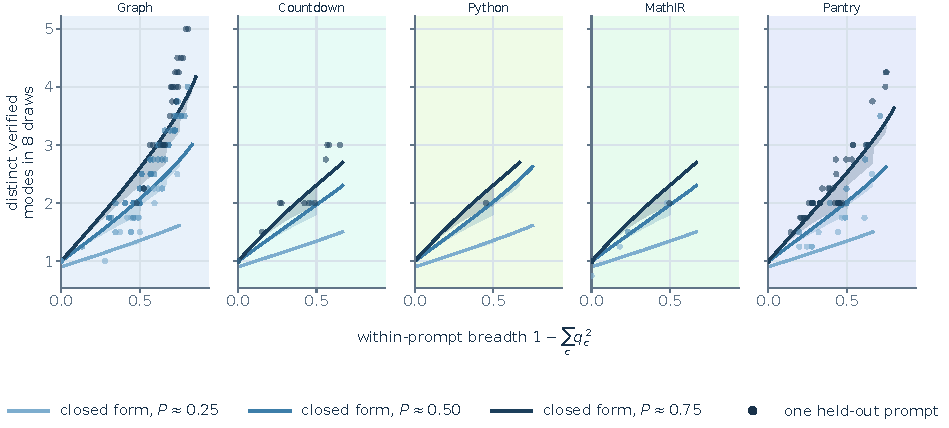
\includegraphics[width=.86\linewidth]{figures/replay_bank_decomposition.pdf}
  \caption{\textbf{Uniform allocation maximizes sampled diversity at fixed buffered probability mass.}
  The horizontal axis traces allocations from a single mode to a uniform
  distribution over $k$ buffered keys. Dashed curves show $1-(1-P)^8$, the
  probability of sampling at least one buffered key when their total mass is
  $P$. Solid curves show the expected number of distinct buffered keys for
  $P\in\{.25,.50,.75\}$; bands span a range of mode counts based on the
  observed prompts and are analytic ranges rather than confidence intervals.
  Points show held-out Level-1 prompts, which have no replay buffer, evaluated
  at the final Re:Dr and
  Re:Max checkpoints of Qwen2.5-0.5B, using one matched seed and grouping
  prompts by their verified response fraction. Their horizontal coordinates
  use empirical key frequencies in $1-\sum_c q_c^2$, rather than the unbiased
  pair estimator. Both coordinates use the same sampled responses, so the
  scatter illustrates agreement with the analytic relationship rather than
  an independent prediction of diversity on new responses.}

  \label{fig:replay-bank-decomposition}
\end{figure}

These properties describe the categorical objective on training-prompt buffers.
Generalization is measured on held-out prompts, whose responses never enter
the buffers. The surrogate alone does not establish that the implemented
response-level objective increases held-out \pmd{}.

% Shared long-paper and workshop benchmark/protocol appendix.

\clearpage
\phantomsection
\begin{center}\large\textbf{Part II. Benchmark and method}\end{center}
\addcontentsline{toc}{part}{Part II. Benchmark and method}

\section{Benchmark and Evaluation Protocol}
\label{app:data}
\label{app:experimental-design}
\label{app:domain-overview}
\label{app:data-inventory}

\mb{} uses a single executable validator to determine correctness and
solution identity, through the map $V(\cdot,s_x)$ defined in
App.~\ref{app:metric-details}. Invalid outputs receive reward zero and no
key; valid outputs receive reward one and a canonical execution key. The
valid-key catalogue and its size are unavailable to the learner and are not
used to schedule replay or determine when training stops.
Table~\ref{tab:tasks} summarizes the five domains and the response variants
that share a key. The datasets are available in the
\href{https://huggingface.co/datasets/od2961/ModeBench}{public release};
the training comparisons in this paper cover Levels 1--3.

\begin{table}[!htbp]
  \centering
  \caption{\textbf{Executable solution identities in the five \mb{} domains.}
  The validator determines both correctness and identity, while the catalogue
  of valid modes is unavailable during training. \emph{Valid modes} reports
  the mean and range of certified catalogue sizes over the Level-1 evaluation
  split. These catalogues need not include every accepted output:
  \texttt{Countdown}, for example, accepts valid keys outside its enumeration.
  \emph{Reached} reports mean distinct verified modes from one hosted
  deployment using 512 draws on 32 prompts
  per domain (Fig.~\ref{fig:gpt56-sampling-budget}). These prompts were
  selected from the evaluation split independently of model outputs. The two
  columns therefore summarize the full split and a subset, respectively.
  \texttt{MathIR}'s catalogue includes longer derivations; limited observed
  coverage does not establish whether these routes are inaccessible or simply
  too rare to observe at the given budget. Higher levels have different
  constructions and mode-count distributions (App.~\ref{app:data-levels}).
  The full prompts and model-specific chat templates appear in App.~\ref{app:prompts}.}

  \label{tab:tasks}
  \scriptsize
  \setlength{\tabcolsep}{5pt}
  \renewcommand{\arraystretch}{1.08}
  \begin{tabularx}{\linewidth}{@{}l
      >{\hsize=1.3\hsize}Y
      >{\hsize=.8\hsize}Y
      >{\hsize=.9\hsize}Y
      rr@{}}
    \toprule
    \textbf{Domain} & \textbf{Generated answer / check} &
    \textbf{Executed key} & \textbf{Equivalent responses} &
    \textbf{Valid modes} & \textbf{Reached} \\
    \midrule
    \texttt{Graph} coloring & Complete assignment; check fixed colors and edges &
    Color vector & Spacing only & 6.27 & 2.53 \\
      & & & & {\scriptsize4--12} & \\
    \addlinespace[2pt]
    \texttt{Countdown} & Parse operands; execute exactly &
    Normalized AST & Commutative order & 4.52 & 3.47 \\
      & & & & {\scriptsize2--8} & \\
    \addlinespace[2pt]
    \texttt{Python} factors & Execute restricted lambda externally &
    Return vector & Programs with the same return vector & 229.44 & 3.75 \\
      & & & & {\scriptsize16--1{,}512} & \\
    \addlinespace[2pt]
    \texttt{MathIR} & Execute bounded action program &
    State trajectory & Programs with the same states & 5.00 & 1.91 \\
      & & & & {\scriptsize5} & \\
    \addlinespace[2pt]
    \texttt{PantryPlan} & Exact ingredient allocation; check all bounds &
    Ingredient support & Quantity and ordering aliases & 18.19 & 6.91 \\
      & & & & {\scriptsize8--40} & \\
    \bottomrule
\end{tabularx}
\end{table}


\subsection{Solution mode definitions and concentration by domain}
\label{app:mode-keying}

\mb{} defines solution modes through three kinds of executable identity.
In \texttt{Countdown} and \texttt{MathIR}, distinct modes are different routes to the same
answer. In \texttt{Python}, they are different return vectors on the public test
inputs. In \texttt{Graph} and \texttt{PantryPlan}, they are different valid answers. The
response budgets also differ (Table~\ref{tab:run-contract}): a \texttt{PantryPlan}
response is a short plan, while a \texttt{Countdown} response is a derivation.
These keys identify verified solutions, not latent reasoning processes.

\paragraph{Sensitivity to the chosen equivalence.}
The canonical key determines which responses count as distinct solutions.
A coarser, task-relevant equivalence can therefore change the measured
diversity gain. App.~\ref{app:coarser-keys} tests one such equivalence per
domain. Most contrasts persist, but the replay gain for Level-3
\texttt{Python} with the original wording falls from $.419$ to zero when
$d$ and $n/d$ are treated as the same unordered factor pair. Among the five
domains, \texttt{Python} is the most sensitive to this choice. Evidence that
the gain extends beyond the original key definitions comes from the other
domains. Training uses the original canonical keys throughout; the coarser
analysis measures sensitivity to alternative definitions of solution identity.

\paragraph{Answer-only training prompts.}
The training prompts request only the final answer
(App.~\ref{app:prompts}), with response budgets chosen accordingly.
Restricting outputs to executable answers allows the validator to determine
solution identity directly, without a learned judge or an embedding-similarity
threshold. The finite solution catalogues also provide the reference values
in Table~\ref{tab:absolute-support-references}. For example, uniform sampling
over the 64 ingredient-selection bit masks in \texttt{PantryPlan} reaches
more verified modes than any trained policy evaluated here.

The training experiments do not measure diversity in long reasoning traces.
The separate hosted-model evaluations include reasoning-enabled deployments
and also exhibit concentration (App.~\ref{app:hosted-mode-diversity}), but
these inference-only observations do not establish how training changes
reasoning behavior.

Across RLVR-only arms, the mean initial-to-terminal increase in conditional
collision is $+0.202$ for route-keyed domains over
98 seed-blocks, $+0.201$ for the behavior-keyed
domain over 15, and $+0.404$ for answer-keyed
domains over 106. All three grouped means increase, with the
largest increase in the answer-keyed group. These comparisons describe
concentration under each definition; differences between domains do not
isolate the effect of choosing a particular key.

\texttt{Countdown}'s mean collision increase is $+0.383$ over
46 seed-blocks, compared with $+0.230$ in \texttt{Graph}.
Thus concentration also occurs among different derivations of a common
answer. \texttt{MathIR} has a smaller increase, $+0.042$. Its certified
catalogue includes longer derivations that are absent from the observed
outputs (App.~\ref{app:algorithm-identity}). Their absence at the evaluated
budgets does not establish that those modes are unreachable.

\paragraph{Explicit-reasoning settings and observed solution counts.}
App.~\ref{app:hosted-reasoning-control} compares five deployments on the
same 480 prompts, with eight responses per prompt and an 8,192-token output
cap in both conditions. Disabling explicit reasoning through the provider
interface lowers overall mean \texttt{distinct@8} in all five deployments:
GPT-5.6 Sol changes from 1.62 to 0.99 and GPT-5.4 from 1.85 to 1.18.
These counts include unsolved prompts and depend on both correctness and
allocation among verified solution modes. Changes in success-conditional
\pmd{} differ across deployments, so lower raw counts do not establish a
common increase in conditional concentration. The requested setting does
not establish the absence of hidden computation, and collection times and
provider defaults can also differ. This comparison therefore describes
solution distributions under the tested configurations, without identifying
an isolated effect of internal deliberation.

\subsection{Dataset splits and validation}
\label{app:data-materialization}

Each domain has disjoint training and evaluation splits
(Table~\ref{tab:run-contract}). \texttt{PantryPlan} and Level 2 also include
separate development splits (App.~\ref{app:data-levels}). For every
\texttt{Python} problem, execution verifies at least two functions with
distinct valid return vectors. For \texttt{MathIR}, each catalogue route is
checked with the same interpreter used to evaluate model outputs.

\begin{table}[!htbp]
\centering
\caption{\textbf{Dataset sizes and certified mode counts.} \texttt{Python} and \texttt{MathIR}
use disjoint training and evaluation splits. Catalogue ranges refer to the
training split; Table~\ref{tab:tasks} gives evaluation-split counts.}

\label{tab:materialization-identities}
\small
\begin{tabular}{@{}lrr@{}}
\toprule
& \textbf{\texttt{Python} factors} & \textbf{\texttt{MathIR} action menu} \\
\midrule
Training problems & 384 & 384 \\
Evaluation problems & 128 & 128 \\
Certified modes per prompt (train) & 16--3{,}600 & 5 \\
\bottomrule
\end{tabular}
\end{table}

\paragraph{\texttt{PantryPlan}.}
\label{app:data-pantry}
\texttt{PantryPlan} contains 384 training, 64 development, and 128 evaluation
prompts across four problem families. The number of feasible ingredient
supports ranges from 8--45 in training and
8--40 in evaluation, with an evaluation mean of
18.19. The validator checks inventory, serving increments, mass,
nutrient bounds, and dietary restrictions using exact arithmetic. The solution
key records which ingredients are used. These checks establish satisfaction
of the stated constraints; they do not assess taste, preparation feasibility,
or food safety.

\subsection{\texttt{Python} execution and validation}
\label{app:python}
\label{app:python-language}

After removing surrounding whitespace, the validator parses each candidate
as a Python expression, with limits of 240 characters and 64 abstract syntax
tree (AST) nodes. The accepted form is \texttt{lambda n: EXPR}, with one
ordinary argument named \texttt{n} and no default value, positional-only,
keyword, or variadic arguments. Integer literals have absolute value at most
10,000. Permitted expressions use \texttt{n}, addition, subtraction,
multiplication, floor division, remainder, integer comparisons, Boolean
\texttt{and}/\texttt{or}, unary plus/minus/\texttt{not}, and conditionals.
The validator rejects Boolean and non-integer literals, calls, imports,
attributes, comprehensions, containers, subscripts, assignment, loops, and
other identifiers.

The task specification contains $J$ distinct integers in $[4,1000]$, with
$2\le J\le8$. Every Level-1 problem uses 4 inputs drawn from
$[6,96]$ and admits at least two valid return vectors.

\paragraph{External execution.}
\label{app:python-process}
Candidate expressions run in an isolated Python process with an empty
\texttt{\_\_builtins\_\_} environment. The process repeats the syntax checks
and evaluates the function on the fixed inputs, subject to a 0.25-second
execution limit and a one-second response deadline. Timeouts, execution errors,
malformed results, non-integer outputs, and failed divisor checks produce
$\bot$ and zero reward. Only a validated integer return vector receives a key.

\paragraph{Behavioral identity.}
\label{app:python-identity}
For each of the $J$ fixed inputs $n_j$, the returned $d_j$ must be an integer
but not a Boolean, satisfy $1<d_j<n_j$, and divide $n_j$ exactly. All checks
must pass. The key is the ordered return vector $(d_1,\ldots,d_J)$;
two programs share a key exactly when these vectors agree. The exact support count
$\prod_j|\{d:1<d<n_j,\ d\mid n_j\}|$ is used only for dataset validation.

\subsection{Matched level constructions}
\label{app:data-levels}

Levels 2--5 expand the search space while preserving the verifier,
canonicalizer, and solution-mode definition. Level 2 is harder for the same
model; Levels 3--5 are calibrated against a fixed Level-1 reference using
larger models, with an exception for Level-4 \texttt{MathIR}.

\paragraph{Level 2.}
Level 2 contains 384 training, 128 development, and 128 evaluation problems,
with no shared problem identities across its splits or with Level 1.
The training distribution of valid-key counts matches that of Level 1.
For \texttt{Graph}, \texttt{Countdown}, \texttt{Python}, and \texttt{MathIR},
the development and evaluation distributions match separate Level-1 reference
sets used for dataset construction. \texttt{PantryPlan} uses its existing
Level-1 splits as references; its 64-prompt development histogram is scaled
by two to define the target counts for the 128-prompt Level-2 development set.

The Level-1 construction reference sets differ from the evaluation sets used
to compare trained policies. Consequently, those evaluation sets have different
valid-key-count distributions across levels in \texttt{Graph},
\texttt{Countdown}, and \texttt{Python}. Cross-level differences reflect both
problem structure and evaluation population, and cannot isolate difficulty
at a fixed distribution of mode counts. Within each level, replay and control
conditions use the same prompts, seeds, fresh-sample objective, and training
budget.

\begin{table}[!htbp]
\centering
\caption{\textbf{Structural differences between Levels 1 and 2.}
The verifier, canonicalizer, and definition of a solution mode are unchanged;
Level 2 expands the search space.}
\label{tab:level2-structure}
\small
\begin{tabularx}{.96\linewidth}{@{}lYY@{}}
\toprule
\textbf{Domain} & \textbf{Level 1} & \textbf{Level 2 structural change} \\
\midrule
\texttt{Graph} coloring & Three hidden vertices & Four hidden vertices \\
\texttt{Countdown} & Three operands & Four operands, with values up to 14 \\
\texttt{Python} factors & Four executed cases, all at most 96 & Four cases, including a value above 96 \\
\texttt{MathIR} & One-sided linear families & Variable-on-both-sides families \\
\texttt{PantryPlan} & Base dietary/composition constraints & More active dietary exclusions and tighter composition \\
\bottomrule
\end{tabularx}
\end{table}

On every domain's development split, fixed Qwen2.5-0.5B has
\texttt{pass@8} in $[.10,.90]$, below its Level-1 construction reference
when both levels use identical decoding settings.

\paragraph{Scale-calibrated Level 3.}
Level 3 is calibrated using Qwen2.5-3B, with Qwen2.5-0.5B on Level 1 as the
reference. Model weights remain fixed. Construction parameters are fitted
on development problems and assessed on held-out prompts. In every domain,
the calibration requires absolute differences from the reference of at most
$.04$ in pass@1 and $.08$ in pass@8, measured using four independent groups
of eight samples per prompt. \distk{} is excluded from the fitting objective.

Both models use their native chat templates, temperature 1, top-$p$ 1, and a
192-token generation limit. \texttt{Graph} prompts request only a boxed final
answer. The other domains receive task-specific solution guidance and use
decoding constrained to legal output syntax, without filtering candidates by
correctness. These criteria establish an empirical match to the reference
success rates rather than a formal two-sided equivalence test.
The Level-3 \texttt{Python} hint ablation removes the strategy guidance
(App.~\ref{app:prompt-hint-ablation}); its difficulty is therefore outside
the scope of this calibration.

\paragraph{Levels 4 and 5.}
Levels 4 and 5 are calibrated with 7B and 14B models, respectively, against
the same Qwen2.5-0.5B Level-1 reference, using pass@1 and pass@8 tolerances
of $.04$ and $.08$.
Level 5 meets these criteria in all five domains. Level 4 meets them in \texttt{Graph},
\texttt{Countdown}, \texttt{Python}, and \texttt{PantryPlan}, but not \texttt{MathIR}.

For \texttt{MathIR}, the reference pass@8/pass@1 ratio is $5.50$, whereas
the largest ratio among the evaluated 7B constructions is $4.16$. A ratio
of mixture means cannot exceed the largest component ratio, so mixing these
constructions cannot reproduce the reference ratio exactly.

The heterogeneity gap, $1-(1-\bar P)^8-\overline{\texttt{pass@8}}$, compares
observed pass@8 with its value if every prompt had the same correctness
$\bar P$. The measured gaps are $.169$--$.398$ at 7B and $.060$ for the
reference. Because the gap depends on mean correctness $\bar P$, these values
are not directly comparable across correctness levels. Each Level-4 domain
contains 384 training, 128 development, and 128 evaluation prompts, disjoint
from other levels. Level-4 \texttt{MathIR} appears in
Figs.~\ref{fig:base-levels-all-scales} and~\ref{fig:level-construction}
but is not difficulty-matched to the reference.

\subsection{Model performance across all five levels}
\label{app:base-levels-all-scales}

Fig.~\ref{fig:base-levels-all-scales} compares Qwen2.5-Instruct across five
levels and domains; Fig.~\ref{fig:families-appendix} adds three model families,
for 375 model--domain--level measurements before benchmark training.
Each measurement uses the same 128 held-out prompts per domain and level,
with four independent groups of eight responses per prompt, totaling 4,096
responses. For \texttt{pass@8} and \distk{}, we score each group, average
within prompts, and then average prompts. For \pmd{}, we pool the four
groups within each prompt (App.~\ref{app:metric-sampling}).

Evaluation uses native chat templates, temperature 1, top-$p=1$, and a
192-token output limit. \texttt{Graph} prompts request boxed final answers;
other domains use task-specific solution guidance and syntax-constrained
decoding. These settings differ from the training evaluations: under the
training template and its larger sample, the same untrained Level-1
\texttt{Python} model defines \pmd{} on 73 of 128 prompts, with mean $.168$
(Section~\ref{sec:results-collapse}). Training effects are therefore measured
against the untrained model under the corresponding evaluation conditions.

Success does not necessarily decrease monotonically with level.
\texttt{pass@8} at the highest evaluated level is below its Level-1 value in
33 of 35 model--domain series. Model scale and
benchmark level also affect diversity differently: the median range of
\pmd{} across scales at a fixed level is .251, compared with
.104 across levels at a fixed scale.

\begin{figure}[!htbp]
  \centering
  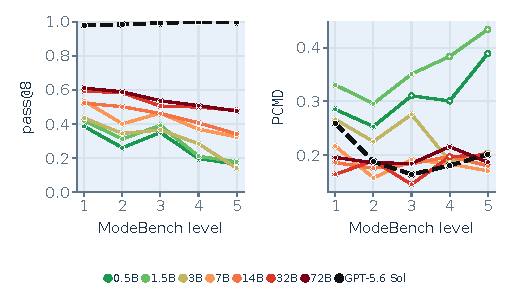
\includegraphics[width=.62\linewidth]{figures/qwen_level_trends.pdf}
  \caption{\textbf{Accuracy and solution diversity vary differently across benchmark levels.}
  Left: \texttt{pass@8}; right: \pmd{}, averaged with equal domain weights
  for each Qwen2.5-Instruct scale (colored lines) and GPT-5.6 Sol (black dashed
  line). This Qwen evaluation augments the 128 held-out prompts with the 384
  training-split prompts where available; none were used to train these
  checkpoints. Filled diversity markers indicate at least 30 prompts with
  two or more correct responses in every domain. Hollow markers average the
  available estimates when at least one domain has insufficient support;
  the set of contributing domains can differ when an estimate is undefined.}

  \label{fig:qwen-level-trends}
\end{figure}

\begin{figure}[!htbp]
  \centering
  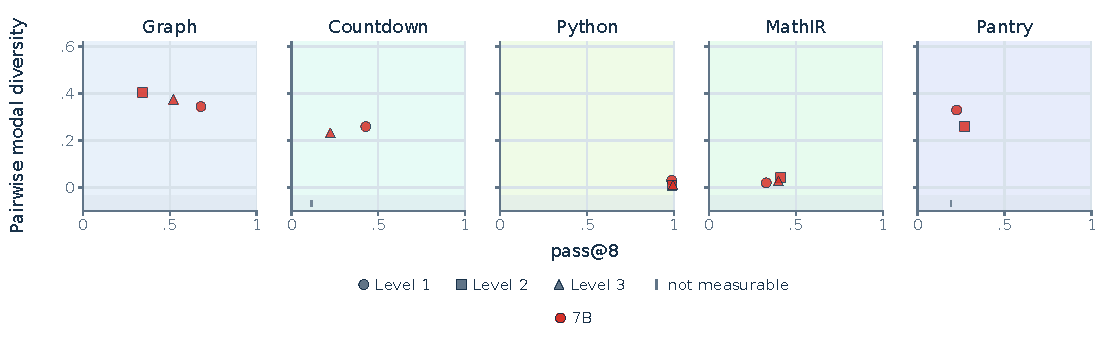
\includegraphics[width=\linewidth]{figures/mode_diversity_level_construction.pdf}
  \caption{\textbf{High accuracy can coexist with low solution diversity.}
  Each row shows one checkpoint before benchmark training, with domains in
  columns, \texttt{pass@8} on the horizontal axis, and \pmd{} on the vertical
  axis. Color indicates parameter count and marker shape indicates level.
  Each measurement uses four groups of eight responses to 128 held-out
  prompts at temperature 1; \pmd{} pools the groups within each prompt.
  Filled markers indicate at least 30 prompts with two or more correct
  responses. Hollow markers indicate 5--29 such prompts and show one standard
  error. Ticks below the axis mark measurements with fewer than five eligible prompts.}

  \label{fig:level-construction}
\end{figure}

\begin{figure}[!htbp]
  \centering
  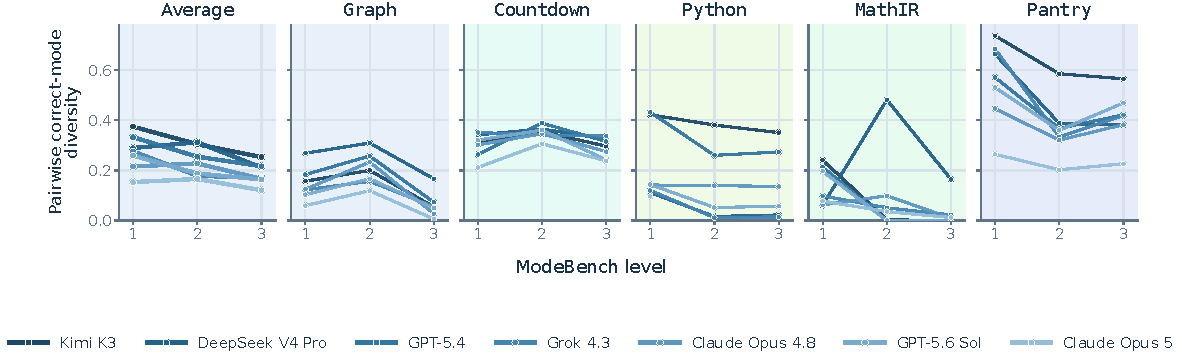
\includegraphics[width=\linewidth]{figures/frontier_level_grid.pdf}
  \caption{\textbf{Mean solution diversity is lower at Level 3 than at Level 1 for every evaluated hosted deployment.}
  Lines show \pmd{} for 7 deployments, with eight
  responses to each of 128 held-out prompts per domain and level. Panels show
  individual domains and their equally weighted mean. For each deployment,
  the set of domains contributing to the mean is fixed across levels.
  Darker lines indicate higher overall diversity. Hollow markers fall below
  the 30-prompt support threshold and are excluded from connecting lines.
  Higher levels change problem structure and add strategy guidance in
  \texttt{MathIR}, \texttt{Python}, and \texttt{PantryPlan}
  (App.~\ref{app:prompt-hint-ablation}); these curves reflect both changes.}

  \label{fig:frontier-level-grid}
\end{figure}

\begin{figure}[!htbp]
  \centering
  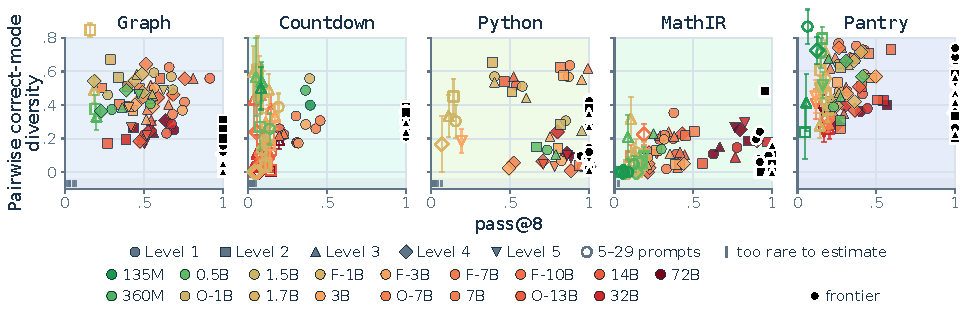
\includegraphics[width=.92\linewidth]{figures/mode_diversity_families_appendix.pdf}
  \caption{\textbf{Models of similar size can differ in solution diversity.}
  SmolLM2, Qwen2.5, Falcon3, and OLMo-2 checkpoints are compared by
  \texttt{pass@8} and \pmd{} across five domains and the available levels,
  before benchmark training. Color indicates parameter count on a logarithmic
  scale; marker shape indicates level. Black markers show the
  7 hosted deployments. Local models use four groups
  of eight responses to 128 held-out prompts per domain and level; hosted
  deployments use eight responses per prompt. Filled markers indicate at
  least 30 prompts with two or more correct responses. Hollow markers
  indicate 5--29 and show one standard error. Ticks below the axis indicate
  fewer than five eligible prompts, for which no diversity estimate is reported.}

  \label{fig:families-appendix}
\end{figure}


\FloatBarrier
\subsection{Other model families at matched scale}
\label{sec:families-appendix}

Fig.~\ref{fig:families-appendix} compares SmolLM2, Qwen2.5, Falcon3, and
OLMo-2 on the same 128 held-out prompts per domain and level. All use four
groups of eight responses, the same verifier, and the same eligibility
thresholds. Comparisons across families use the 4 shared
levels; only Qwen2.5 is evaluated at Level 5. Color denotes parameter count.

Families differ in diversity even at similar parameter counts. Near 7B,
Qwen2.5, Falcon3, and OLMo-2 have different \pmd{} values despite similar
\texttt{pass@8}. Their ordering persists in the 10--15B range, where Falcon3
and OLMo-2 are close. Within parameter-count bands, the median range of
\pmd{} across family means is .166, compared with
.198 across scales within a family, over the
4 shared levels. The earlier .251 summary instead
compares all seven Qwen scales at each level. These descriptive comparisons
do not isolate which pretraining or post-training choices account for the
differences between models.

\clearpage
\subsection{Training and evaluation settings}
\label{app:repro-run-contract}
\label{app:comparison-design}

% [H] pinned this table to the head of the subsection, and being too tall for
% what the previous page had left it took a page of its own and stranded the
% remainder. Floating lets the prose that follows it close the gap.
\begin{table}[!htbp]
  \centering
  \caption{\textbf{Paired comparisons use the same numbers of optimizer updates and fresh rollouts.}
  Treatment and control share the settings below. Both compute replay scores
  and execute the backward pass, but the replay gradient is exactly zero in
  the control. Their buffer contents can differ, so replay workloads, total
  floating-point operations, and wall-clock time are not matched. The control
  receives no additional training in place of replay computation
  (App.~\ref{app:compute-matching}).}

  \label{tab:run-contract}
  \small
  \begin{tabularx}{\linewidth}{@{}P{.23\linewidth}Y@{}}
    \toprule
    \textbf{Component} & \textbf{Setting} \\
    \midrule
    Data & 384 training and 128 disjoint evaluation prompts per domain and
      level; evaluation prompts are excluded from training and replay. \\
    Fresh rollouts & $G=16$, temperature 1, top-$p=1$; one prompt group per update. \\
    Optimization & Eight training passes (3,072 updates), with one PPO epoch
      per batch. $\beta_{\mathrm{KL}}=0$ except in the reference-KL comparison
      (App.~\ref{app:kl-measured}), which varies only this coefficient.
      Paired conditions share initialization, prompt order, optimizer,
      hardware class, and checkpoint frequency. \\
    Evaluation & At passes $0,.5,\ldots,8$: four groups of eight responses
      per prompt at temperature 1 and top-$p=1$, plus a separate greedy
      response at temperature 0. Final comparisons use the last checkpoint. \\
    Replay & Capacity $M=16$ keys per prompt; buffers are selected in
      round-robin order, one per update; $\lambda_{\mathrm{replay}}=.10$.
      The control has zero replay gradient; buffer contents and computational
      workloads may differ between conditions. \\
    Training seeds & Five per model--domain combination; paired comparisons use
      common seeds, with sample sizes reported alongside the results. \\
    Learning rate & Qwen2.5-0.5B and Falcon3-1B: constant $2\times10^{-7}$,
      with Falcon optimizer states stored on the CPU. Qwen2.5-3B: cosine
      decay from a $10^{-7}$ peak to a $10^{-8}$ floor, with 10\% warmup. \\
    Optimizer & Fused Adam in \texttt{bf16} with decoupled weight decay,
      $\beta_1=.9$, $\beta_2=.95$, weight decay $0$, gradient-norm clip $1.0$,
      with gradient checkpointing. CPU offloading uses the corresponding
      CPU optimizer implementation with the same hyperparameters. \\
    Policy update & Parameters are synchronized after every update, and each
      rollout is used once in a single PPO epoch. The symmetric clipping
      threshold is $\varepsilon=.2$. The importance ratio equals $1$ when
      the surrogate is evaluated in this update scheme, so clipping is inactive. \\
    % All twelve cells are the OAT_ZERO_GENERATE_MAX_LENGTH actually submitted,
    % read per domain from the job ledgers rather than from a launcher default:
    %   0.5B  var/artifacts/e72_frontier_source_runs.json
    %           (inherited_eval_config.generate_max_length; the 3B cohort
    %            inherits this record and overrides only the base model)
    %   1B    var/artifacts/e79_falcon1b_aligned_verified_replay_jobs.json
    %   3B    var/artifacts/e80r1_qwen3b_aligned_verified_replay_jobs.json
    % ops/train.sh defaults this to 192, so a domain that is 192 looks the same
    % whether it was chosen or inherited; the ledgers are what distinguish them.
    Response tokens & \texttt{Graph} and \texttt{Countdown}: 192; \texttt{Python}: 192/512/192
      at 0.5B/1B/3B; \texttt{MathIR}: 64/128/64; \texttt{PantryPlan}: 8. \\
    \bottomrule
  \end{tabularx}
\end{table}



For each training seed, \texttt{pass@8} and \texttt{distinct@8} are averaged
over four eight-response groups per prompt and all 128 evaluation prompts;
\texttt{mean@8} is the fraction of correct responses. Responses are independent
within a group. Independence across groups, required for the pooled \pmd{}
interpretation, depends on the sampling procedure described in
App.~\ref{app:metric-sampling}. Evaluation outputs are excluded from training
and replay, and do not determine checkpoint selection or stopping.

Comparisons use paired final checkpoints. Comparisons with five matched
training seeds use nominal pointwise 95\% Student-$t$ intervals; other main
checkpoint comparisons report sample sizes and descriptive means. Diversity
comparisons use the prompt-eligibility thresholds and interval procedures
specified alongside their results. Intervals condition on the fixed evaluation
prompts and sampled responses. The replay-weighting comparison instead uses
a bootstrap over paired training seeds.

% Finish benchmark floats before beginning the prompt examples.
\FloatBarrier
\section{Exact Domain Prompts}
\label{app:prompts}

Each domain's training prompt contains one system message and one user
message, without few-shot examples. Training and evaluation use the same
template within each method. The examples below reproduce the first prompt
from each Level-1 evaluation split in Qwen's chat format. Falcon3 uses the
same message text with its own \texttt{<|system|>} and \texttt{<|user|>}
markers. Models evaluated before benchmark training use their tokenizer's
native chat template (App.~\ref{app:base-levels-all-scales}).
App.~\ref{app:data-levels} describes the different problems and prompting
conditions at Levels 2--5.

The examples preserve the prompt text. A continuation line indented by two
spaces indicates a display line break; replacing that break and indentation
with one space recovers the original text. In the \texttt{PantryPlan}
example, a line break without this indentation is part of the prompt.

% BEGIN generated by ops/check_paper_domain_prompts.py

\filbreak
\subsection{\texttt{Graph} coloring}
\label{app:prompt-graph}

\noindent 384 training and 128 evaluation prompts.

\begin{Verbatim}[fontsize=\scriptsize,frame=single,framesep=4pt,rulecolor=\color{black!25},samepage=true]
<|im_start|>system
Return only the final answer inside \boxed{}. Do not explain.<|im_end|>
<|im_start|>user
Color this graph with vertices 1 through 6. The undirected edges are: (1,2), (1,3),
  (3,5), (3,6), (4,6), (5,6). Assign each vertex one color from {1, 2, 3} so that no
  edge has the same color on both endpoints. A partial coloring is 2??1?2, where ?
  means uncolored. Keep every shown digit fixed. There are exactly 3 question marks.
  Return exactly one final answer and no explanation: exactly 3 digits, each one 1,
  2, or 3, for the missing positions from left to right, inside \boxed{}.<|im_end|>
<|im_start|>assistant
\end{Verbatim}

\filbreak
\subsection{\texttt{Countdown}}
\label{app:prompt-countdown}

\noindent 384 training and 128 evaluation prompts.

\begin{Verbatim}[fontsize=\scriptsize,frame=single,framesep=4pt,rulecolor=\color{black!25},samepage=true]
<|im_start|>system
Return only the final answer inside \boxed{}. Do not explain.<|im_end|>
<|im_start|>user
Using the numbers [3, 6, 9], create an arithmetic expression that equals 18. Use
  each given number exactly once. You may use +, -, *, /, and parentheses. Return
  exactly one final answer and no explanation: the expression inside
  \boxed{}.<|im_end|>
<|im_start|>assistant
\end{Verbatim}

\filbreak
\subsection{\texttt{Python} factors}
\label{app:prompt-python}

\noindent 384 training and 128 evaluation prompts.

\begin{Verbatim}[fontsize=\scriptsize,frame=single,framesep=4pt,rulecolor=\color{black!25},samepage=true]
<|im_start|>system
Return only the final answer inside \boxed{}. Do not explain.<|im_end|>
<|im_start|>user
Write one pure Python function with the exact form lambda n: EXPR. An external
  Python tool will call it once for each n in [18, 82, 91, 93]. For every call,
  return an integer d satisfying 1 < d < n and n % d == 0. Different valid return
  vectors are different solution modes. You may use integer literals, n, +, -, *,
  //, %, comparisons, Boolean operators, and conditional expressions; calls,
  imports, attributes, containers, and other names are forbidden. Return exactly the
  one-line lambda inside \boxed{} and no explanation.<|im_end|>
<|im_start|>assistant
\end{Verbatim}

\filbreak
\subsection{\texttt{MathIR} action menu}
\label{app:prompt-mathir}

\noindent 384 training and 128 evaluation prompts.

\begin{Verbatim}[fontsize=\scriptsize,frame=single,framesep=4pt,rulecolor=\color{black!25},samepage=true]
<|im_start|>system
Return only the final answer inside \boxed{}. Do not explain.<|im_end|>
<|im_start|>user
MathIR linear-menu-v1. Solve for x by choosing an executable action sequence. Every
  selected action is applied exactly to BOTH sides of the current equation, followed
  by exact simplification. Bindings: a=2, b=-9, c=-1. Initial equation: x/a + b = c.
  Action menu: A means div(a); B means add(b); C means sub(b); D means sub(c); E
  means sub(mul(a,b)); F means mul(a). Choose 1-4 action IDs. Illegal operations,
  repeated states, and paths that do not finish with x isolated are rejected. Return
  only the IDs separated by semicolons inside the answer box; for example formatting
  only: \boxed{A;C}. Do not return x's numeric value.<|im_end|>
<|im_start|>assistant
\end{Verbatim}

\subsection{\texttt{PantryPlan}}
\label{app:prompt-pantry}

\noindent 384 training and 128 evaluation prompts.

\begin{Verbatim}[fontsize=\scriptsize,frame=single,framesep=4pt,rulecolor=\color{black!25},samepage=false]
<|im_start|>system
Return only six binary digits and no other text. Each digit maps to the
  corresponding Pantry row in printed order. A trusted environment will choose exact
  quantities on precisely the selected rows.<|im_end|>
<|im_start|>user
Create one feasible high fiber snack from this frozen pantry.
Nutrition values are per 100 g. Quantities are exact integer grams.

Pantry:
- almonds: available=100g, step=25g, minimum-if-used=50g; energy=584kcal,
  protein=21.5g, fiber=10.8g, sodium=0.0mg; tags=tree_nut
- banana: available=125g, step=25g, minimum-if-used=50g; energy=97.0kcal,
  protein=0.74g, fiber=4.62g, sodium=0.0mg; tags=none
- carrots: available=150g, step=25g, minimum-if-used=50g; energy=45.0kcal,
  protein=0.941g, fiber=3.1g, sodium=86.6mg; tags=none
- grape_tomatoes: available=100g, step=25g, minimum-if-used=50g; energy=27.0kcal,
  protein=0.83g, fiber=2.1g, sodium=6.0mg; tags=none
- navel_orange: available=150g, step=25g, minimum-if-used=50g; energy=47.0kcal,
  protein=0.91g, fiber=2.0g, sodium=9.0mg; tags=none
- sunflower_seeds: available=125g, step=25g, minimum-if-used=50g; energy=571kcal,
  protein=18.9g, fiber=7.22g, sodium=0.0mg; tags=none

Use 2 to 4 ingredients.
Forbidden tags: none
Targets:
- mass_g: minimum 125, maximum 200
- energy_kcal: minimum 239.4, maximum 432.25
- protein_g: minimum 6.423
- fiber_g: minimum 3.478
- sodium_mg: maximum 37.6

Choose the ingredient support as a six-bit mask in the exact Pantry row order. Bit 1
  includes that row and bit 0 excludes it.<|im_end|>
<|im_start|>assistant
\end{Verbatim}

% END generated by ops/check_paper_domain_prompts.py

% Shared exact replay update; empirical comparisons are in results.tex.

\section{Replay Algorithm}
\label{app:algorithm}

Verified replay combines learning from newly sampled responses with a
likelihood loss on stored, verified solutions. Each prompt $x$ has a buffer
$\mathcal B_x$ of at most $M$ exemplars, with one response per canonical key.
A round-robin cursor $\sigma$ selects one prompt's buffer at each update,
and all keys in that buffer contribute equally to the replay loss.
Table~\ref{tab:notation} defines the notation;
App.~\ref{app:replay-metric-alignment} relates this objective to diversity.

\subsection{Fresh task advantages}
\label{app:binary-maxrl}

For a group of $G$ fresh responses with verified binary rewards $R_i$ and
$R=\sum_i R_i$, Dr.GRPO uses $A_i=R_i-R/G$, while MaxRL uses
\[
 A_i^{\mathrm{MaxRL}}=
 \begin{cases}
 G R_i/R-1, & R>0,\\
 0, & R=0.
 \end{cases}
\]
The centered MaxRL estimator \citep{tajwar2026maxrl} assigns advantage $-1$
to failures in mixed groups and gives each success greater weight when
successes are scarce. Both objectives assign zero task advantage to every
response in an all-correct or all-failure group. Lemma~\ref{lem:maxrl-mean}
derives MaxRL's mean objective as a harmonic combination of pass@\(k\)
terms. These advantages apply to fresh responses; stored exemplars contribute
through the separate replay loss.

\subsection{Optimizer update}
\label{app:algorithm-update}

\begin{algorithm}[H]
  \caption{\textbf{Verified replay update.} The fresh objective selects Re:Dr or Re:Max.}
  \label{alg:verified-replay-update}
  \small
  \begin{algorithmic}[1]
    \REQUIRE Policy $\pi_\theta$; prompt $x$ and verifier specification
      $s_x$; group size $G$; fresh objective
      $o\in\{\mathrm{MaxRL},\mathrm{Dr.GRPO}\}$; replay weight
      $\lambda_{\mathrm{replay}}$; buffer capacity $M$; buffers and cursor
      $(\mathcal B,\sigma)$
    \ENSURE Updated $(\theta',\mathcal B',\sigma')$
    \STATE Draw the on-policy group
      $\mathcal G=\{y_i\sim\pi_\theta(\cdot\mid x)\}_{i=1}^G$
    \FOR{$i=1,\ldots,G$}
      \STATE Execute $\widetilde c_i\gets V(y_i,s_x)$ and observe task
        reward $R_i$
      \STATE Set $c_i\gets\widetilde c_i$ iff
        $R_i>0\wedge\widetilde c_i\ne\bot$; otherwise set $c_i\gets\bot$
    \ENDFOR
    \STATE Compute fresh task advantages $A_i^{o}$ from $\{R_j\}_{j=1}^G$;
      for $o=\mathrm{MaxRL}$ use the formula in App.~\ref{app:binary-maxrl}
    \STATE After the full group is validated, deterministically retain one
      policy exemplar for each new $c_i\ne\bot$ in $\mathcal B_x$, up to
      capacity $M$
    \STATE $(z,\sigma')\gets\textsc{NextBuffer}
      (\{\mathcal B_u\}_u,\sigma)$ by a fixed round-robin cursor over
      prompts; the replayed prompt $z$ need not be the prompt $x$ that
      supplied the fresh group
    \IF{a replay buffer $\mathcal B_z$ exists}
      \STATE For each exemplar $e_c\in\mathcal B_z$, compute
        $\ell_c=|e_c|^{-1}\log\pi_\theta(e_c\mid z)$
      \STATE $L_{\mathrm{replay}}\gets-|\mathcal B_z|^{-1}
        \sum_{c\in\mathcal B_z}\ell_c$
    \ELSE
      \STATE $L_{\mathrm{replay}}\gets0$
    \ENDIF
    \STATE Set the replay-loss normalization $w_{\mathrm{rep}}\gets(G-1)/G^2$
    \STATE $\theta'\gets\textsc{Update}
      (\theta,L_{\mathrm{PPO}}(A^{o})
      +w_{\mathrm{rep}}\lambda_{\mathrm{replay}}L_{\mathrm{replay}})$
\end{algorithmic}
\end{algorithm}

\subsection{Buffer construction and scheduling}
\label{app:algorithm-bank}

Each buffer is associated with an exact prompt-token sequence. A response
is eligible for storage if it has positive task reward and a valid canonical
key, including responses that reach the generation limit. The entire group
is validated before the buffer is updated. For each newly observed key, we
retain the lexicographically smallest normalized response-token sequence;
new keys are inserted in sorted order. Selection therefore does not depend
on the order of responses within the group. Each buffer holds at most
$M=16$ exemplars, one per key, with no eviction or replacement. Keys first
observed after the buffer is full receive no replay support.

At each update, a deterministic round-robin schedule selects one nonempty
buffer, including buffers containing a single exemplar. The choice does not
use reward magnitudes, evaluation results, a target mode count, or entropy.
The policy scores every stored response in the selected buffer by teacher
forcing, conditioned on its original prompt. Each exemplar contributes its
mean response-token log probability, excluding prompt and padding tokens.

The replay loss is the negative mean score over the selected keys,
weighted by $\lambda_{\mathrm{replay}}(G-1)/G^2$
(Algorithm~\ref{alg:verified-replay-update}). The normalization $(G-1)/G^2$
matches the weight of a single success in a centered Dr.GRPO group: its
advantage is $(G-1)/G$, followed by averaging over $G$ responses
(Lemma~\ref{lem:grpo-mean}). This loss uses only discovered training
exemplars; it requires neither the complete valid-key catalogue nor
evaluation outputs.

\subsection{Control without replay gradients}
\label{app:algorithm-control}

Replay and control use the same validation, buffer construction, scheduling,
and exemplar-scoring procedures. The control sets the replay gradient to
zero while retaining the forward and backward computations. Both conditions
combine the fresh-task and replay gradients in one optimizer step; the
replay gradient is their only difference in the learning objective.

As the policies diverge, they can generate different responses and accumulate
different buffers, which changes the selected exemplars and their lengths.
The conditions match optimizer updates and fresh-rollout budgets, but not
realized floating-point operations or wall-clock time. The control receives
no additional task-gradient updates, fresh rollouts, or training time in
place of replay computation. The comparison isolates the contribution of the
replay learning signal under this design, without establishing an advantage
at equal total compute (App.~\ref{app:compute-matching}).

\subsection{Verifier requirements and applicability}
\label{app:algorithm-identity}

Replay requires a deterministic rule for grouping verified responses into
solution modes. Its canonical key must be computable for every training
response at reasonable cost and must reflect the task's definition of a
solution. In \mb{}, one executable validator determines both correctness
and identity, so buffer construction requires no learned judge or
embedding-similarity threshold.

Final-answer grading, as used for MATH, GSM8K, and AIME, does not distinguish
derivations of the same answer. When a prompt has only one correct answer,
an answer-based key places every successful response in the same mode. The
buffer then holds one exemplar, and replay reinforces it without balancing
alternative derivations. That buffer is the capacity-one arm of
App.~\ref{app:mode-agnostic-replay}, which retains 58\% of the
Re:Dr diversity effect and a correctness gain of +.263 against
Re:Dr's +.352. Measuring and replaying distinct derivations
requires a finer definition of identity.

\texttt{MathIR} uses executed state trajectories as keys. Its catalogue
includes verified four-state routes, but none appears among 27,450
verified draws. Across 115 solved Level-1 prompts, these
draws cover 67\% of the certified two-state modes and
52\% of the three-state modes. Different modes rarely appear
for the same prompt. Terminal \pmd{} averages .006, corresponding
to 1.01 effective verified modes per prompt. These results provide
limited evidence for diversity gains among alternative derivations.

Across the 6 comparisons, including \texttt{MathIR} in the
five-domain mean reduces the \pmd{} gain by .010--.074
relative to the corresponding four-domain mean. At Qwen2.5-0.5B, the Re:Dr
gain is +.294 across all five domains and +.364 across the other
four. App.~\ref{app:hosted-mode-diversity} reports hosted-model results for
the same four-domain subset.

For open-ended derivations, a learned judge could supply a novelty criterion,
but that criterion would require independent validation. Judge decisions can
be inconsistent or disagree with task correctness, and replay may reinforce
distinctions that the judge rewards without improving solution diversity.
Fixing the judge model, prompt, and decoding rule does not by itself ensure
a valid equivalence relation. Where executable keys are available, they can
be used to assess the judge and measure diversity separately from its training
signal. We do not evaluate judge-based replay here.

\subsection{Exemplar quality and length}
\label{app:algorithm-quality}

Canonical verification establishes that a response satisfies the task
constraints. It does not validate every intermediate reasoning step: a
verified response may be verbose or include an unsound explanation. Replay
weights exemplars by solution key without ranking their reasoning quality.

Each key occupies one buffer entry and contributes its exemplar's mean
response-token log probability,
$\ell_c=|e_c|^{-1}\log\pi_\theta(e_c\mid z)$. Longer responses therefore do
not receive more buffer entries or loss weight proportional to their token
count. This normalization still affects the learning target. In a categorical
surrogate with one exemplar of fixed length $L_b$ per key, the effective
weights are proportional to $L_b^{-1}$. With full coverage, the limiting
distribution favors shorter exemplars and is uniform only when lengths are
equal (App.~\ref{app:theory-replay}). This conclusion concerns the surrogate;
mean-token normalization does not imply uniform key probabilities in a
language model or guarantee concise, sound explanations.

Additional length or reasoning-quality filters would change which exemplars
enter or remain in the buffer, and hence change the replay target. We use no
such filters beyond the stated generation limits and verification rules.
Restricting length can exclude valid alternatives: \texttt{MathIR} includes
longer state trajectories, and the observed lambdas for rarer \texttt{Python}
return vectors are longer than those for the modal vector. Evaluating a
quality filter would therefore require measuring both solution quality and
diversity among retained modes.

\section{Fixed Semantic-MaxEnt Comparator}
\label{app:semantic-maxent}

Fixed Semantic-MaxEnt adds a frequency-based bonus to the fresh-response
advantage. It counts previously observed verified keys but does not optimize
the likelihood of stored exemplars. For response $i$ in a group of $G$
responses to prompt $x$, let $n_x(a)$ count earlier successful responses
with key $a$, and let $m_{-i}(a)$ count successful responses with that key
among the other members of the current group. Write
$N_x=\sum_a n_x(a)$, $S_{-i}=\sum_a m_{-i}(a)\le G-1$, and let
$\mathcal K_i$ contain all keys observed in these two sources. Adding one
pseudocount per observed key and reserving one for unseen keys gives,
for $a\in\mathcal K_i$,

\begin{equation}
  \hat p_i(a)=\frac{n_x(a)+m_{-i}(a)+1}{N_x+S_{-i}+|\mathcal K_i|+1},\qquad
  \hat p_i(\textsc{unseen})=\frac{1}{N_x+S_{-i}+|\mathcal K_i|+1}.
  \label{eq:open-set-predictor}
\end{equation}
A response whose key is outside $\mathcal K_i$ receives the probability
assigned to the unseen category. Invalid and unsuccessful responses do not
contribute to the counts.

\paragraph{Counts and advantage calculation.}
Counts are specific to each exact prompt-token sequence and accumulate
throughout training without decay or reset. Only responses with positive
reward and a valid key are counted. Each response is scored using previous
groups and the other successful responses in its current group. Counts for
the full current group are added only after scoring, so a response never
contributes to its own predicted probability.
The added advantage for an eligible successful response is held constant
during differentiation and equals

\begin{equation}
  A^{\rm sem}_{i,t}=\eta\,
  \frac{\min\{-\log\hat p_i(a_i),\kappa\}
    -\E_{\hat p_i}[\min\{-\log\hat p_i(a),\kappa\}]}{\kappa},
  \qquad \eta=.10,\ \kappa=5.
  \label{eq:legacy-semantic-advantage}
\end{equation}
The same $A^{\rm sem}_{i,t}$ applies at every token position $t$ of response
$i$. Invalid and unsuccessful responses receive zero bonus. The fixed scale
$\eta$ bounds the centered bonus in magnitude, while $\kappa$ clips the
surprisal. The bonus can favor an underrepresented verified mode when that
mode appears in a fresh response, but it adds no direct likelihood term for
a stored exemplar absent from the group. If neither previous groups nor the other
successful responses provide a key, the unseen category has probability one
and the bonus is zero. App.~\ref{app:ucpo-progress} reports the comparison.

\paragraph{Relation to conditional entropy.}

For the true conditional distribution $q_\theta=p_\theta(\cdot\mid\mathcal C)$,
\begin{equation}
 \nabla_\theta H(q_\theta)
 =\E_{a\sim q_\theta}[(-\log q_\theta(a))\nabla_\theta\log q_\theta(a)].
 \label{eq:entropy-score-function}
\end{equation}
The frequency predictor generally does not provide an unbiased estimator
of this gradient. To see the distinction, hold a predictor score vector $s$
and baseline $b$ fixed independently of the scored action, for example by
conditioning on the other responses in its group. Averaging the gradients
of successful responses under the unconditional policy gives

\[
 \E_{Z\sim p}[\1\{Z\in\mathcal C\}(s_Z-b)\nabla_\theta\log p_Z]
 =P\E_{c\sim q}[s_c\nabla_\theta\log q_c]
   +(\E_q[s]-b)\nabla_\theta P.
\]
The predictor's baseline need not equal the current conditional mean
$\E_q[s]$. The second term can therefore change correctness as well as the
allocation among correct modes. Even with the exact, unclipped score
$s_c=-\log q_c$ and baseline $b=H(q)$, averaging over all rollout responses
yields $P\nabla_\theta H(q)$, scaled by the probability of success.

The distinction also matters when only one correct key exists. Its
conditional entropy is zero, yet probability assigned to the unseen
category can make its semantic advantage negative after it has been
observed. The bonus is therefore generally not an exact conditional-entropy
gradient, and it provides no guarantee of individual-mode preservation.

% Every part divider opens a fresh page, this one included. It used to run on
% from the comparator section to save the white space below that section's end;
% uniformity across the seven dividers is worth the part page.
\clearpage
\phantomsection
\begin{center}\large\textbf{Part III. Training results}\end{center}
\addcontentsline{toc}{part}{Part III. Training results}

\section{Empirical Results and Comparisons}
\label{app:supporting}

\begin{figure}[!htbp]
\centering
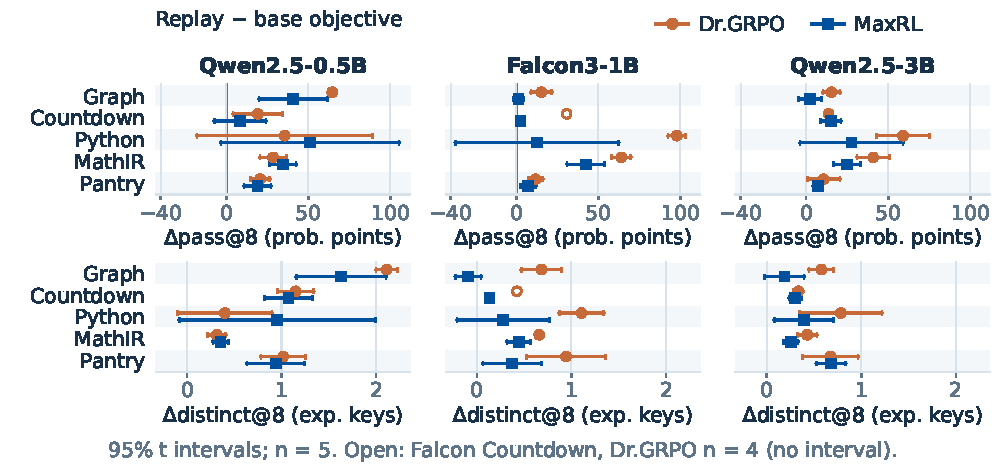
\includegraphics[width=\linewidth]{figures/replay_factorial_effects.pdf}
\caption{\textbf{Replay raises mean correctness at all three model scales.}
Final-checkpoint differences: Re:Dr minus Dr.GRPO (circles) and Re:Max minus
MaxRL (squares), measured in percentage points for \texttt{pass@8} and in
\pmd{} units for diversity. Filled markers use five paired seeds; hollow
markers use fewer. For Re:Dr, correctness uses four seeds in Falcon
\texttt{Countdown}; diversity uses four in Falcon \texttt{Countdown}, one
in Falcon \texttt{MathIR}, and two in Qwen2.5-3B \texttt{Python}. Diversity
requires at least 20 eligible prompts per arm; blanks indicate no eligible
comparison. Bars show nominal paired 95\% Student-$t$ intervals, requiring
five seeds for correctness and at least two for diversity.}
  \label{fig:replay-factorial-effects}
\end{figure}

\subsection{Terminal comparisons across scales}
\label{app:scale-matrix}
\label{app:scale-snapshot}
\label{app:maxrl-scale-extensions}
\label{app:current-campaign-results}

Paired conditions share initialization, training and evaluation prompts,
eight training passes, evaluation requests, the verifier, and replay schedule.
The control uses the same buffer construction and scoring procedures with
zero replay gradient. Policies can develop different buffers and workloads,
so total compute is not matched (App.~\ref{app:compute-matching}).

\crossscaletablematerial

\paragraph{Dr.GRPO retention contrasts.}
\label{app:retention-numerical-detail}

% Floats rather than [H] so it can rise to the page its discussion starts
% on instead of forcing a break and leaving the preceding page part empty.
\begin{table}[!tbp]
  \centering
  \caption{\textbf{Replay improves mean correctness and solution diversity at each tested scale.}
  Final-checkpoint differences between Re:Dr and Dr.GRPO, by domain and
  model. Superscripts indicate fewer than five paired seeds; dashes indicate
  no eligible comparison. Diversity effects require at least 20 eligible
  prompts per arm. Each Avg weights a fixed set of domains equally within
  seed: all five for correctness, and domains eligible for every seed for
  diversity. The diversity mean uses \texttt{Graph} and \texttt{PantryPlan}
  at Falcon3-1B, all domains except \texttt{Python} at Qwen2.5-3B, and all
  five at 0.5B. Eligible prompt subsets may differ between the two arms.}

\label{tab:cross-scale-terminal-effects}
  \scriptsize
  % Keep the two longest domain headers on two lines, as in the main table,
  % so typewriter labels retain their size within the thirteen-column layout.
  \setlength{\tabcolsep}{1.4pt}
  \renewcommand{\arraystretch}{0.92}
  \begin{tabular}{@{}l*{12}{r}@{}}
    \toprule
    & \multicolumn{6}{c}{\textbf{$\Delta$ \texttt{pass@8}}}
      & \multicolumn{6}{c}{\textbf{$\Delta$ \pmd{}}} \\
    \cmidrule(lr){2-7}\cmidrule(l){8-13}
    & \texttt{Graph} & \shortstack{\texttt{Count}\\\texttt{down}} & \texttt{Python} & \texttt{MathIR} & \shortstack{\texttt{Pantry}\\\texttt{Plan}} & Avg
      & \texttt{Graph} & \shortstack{\texttt{Count}\\\texttt{down}} & \texttt{Python} & \texttt{MathIR} & \shortstack{\texttt{Pantry}\\\texttt{Plan}} & Avg \\
    \midrule
    % Generated by build_paper_retention_matrix_tables.py; do not hand edit.
    \qwenmark{}2.5-0.5B & \cellcolor[HTML]{A9D6A0}$+.646$ & \cellcolor[HTML]{C7E0A2}$+.191$ & \cellcolor[HTML]{DBE7A4}$+.356$ & \cellcolor[HTML]{D5E4A3}$+.285$ & \cellcolor[HTML]{A9D6A0}$+.207$ & \cellcolor[HTML]{BCDCA1}$+.337$ & \cellcolor[HTML]{A9D6A0}$+.559$ & \cellcolor[HTML]{A9D6A0}$+.480$ & \cellcolor[HTML]{A9D6A0}$+.082$ & \cellcolor[HTML]{DDE7A4}$+.017$ & \cellcolor[HTML]{A9D6A0}$+.334$ & \cellcolor[HTML]{A9D6A0}$+.294$ \\
    \falconmark{}3-1B & \cellcolor[HTML]{E5EAA5}$+.153$ & \cellcolor[HTML]{A9D6A0}$+.307^{4}$ & \cellcolor[HTML]{A9D6A0}$+.979$ & \cellcolor[HTML]{A9D6A0}$+.640$ & \cellcolor[HTML]{CBE1A3}$+.118$ & \cellcolor[HTML]{A9D6A0}$+.442^{4}$ & \cellcolor[HTML]{D8E6A4}$+.224$ & \cellcolor[HTML]{F3EEA6}$+.032^{4}$ & \textemdash{} & \cellcolor[HTML]{D5E4A3}$+.022^{1}$ & \cellcolor[HTML]{ADD7A0}$+.317$ & \cellcolor[HTML]{AFD8A0}$+.271$ \\
    \qwenmark{}2.5-3B & \cellcolor[HTML]{E5EAA5}$+.154$ & \cellcolor[HTML]{D5E4A3}$+.137$ & \cellcolor[HTML]{C8E0A2}$+.590$ & \cellcolor[HTML]{C6DFA2}$+.409$ & \cellcolor[HTML]{CFE3A3}$+.106$ & \cellcolor[HTML]{C6E0A2}$+.279$ & \cellcolor[HTML]{DFE8A4}$+.176$ & \cellcolor[HTML]{E8EBA5}$+.100$ & \cellcolor[HTML]{CCE1A3}$+.046^{2}$ & \cellcolor[HTML]{E4E9A4}$+.013$ & \cellcolor[HTML]{BEDDA2}$+.247$ & \cellcolor[HTML]{D4E4A3}$+.134$ \\
    \bottomrule

  \end{tabular}
\end{table}

Tables~\ref{tab:core-terminal-endpoints} and~\ref{tab:cross-scale-terminal-effects}
report means for each condition and paired replay effects, respectively.
Adding replay to Dr.GRPO increases mean \texttt{pass@8} and \distk{} in
all 14 comparisons with five paired seeds; \distk{} increases in all 74
individual seed pairs. Because \distk{} also depends on correctness, we use
\pmd{} to measure diversity conditional on a correct response.

For Qwen2.5-0.5B, \texttt{Countdown} \texttt{pass@8} rises from $.480$ to
$.672$, with a \pmd{} gain of $+.480$ (95\% interval $[+.447,+.513]$).
\texttt{Python} correctness rises from $.172$ to $.528$, with a diversity
gain of $+.082$ ($[-.146,+.310]$). \texttt{MathIR} correctness rises from
$.512$ to $.796$, with a diversity gain of $+.017$ ($[+.003,+.031]$).
These are nominal Student-$t$ intervals over five paired training seeds,
without multiple-comparison adjustment. \texttt{Countdown}'s final \pmd{}
values are $.007$ for Dr.GRPO and $.487$ for Re:Dr. Its keys distinguish
computation routes, but these held-out evaluations do not track the survival
of particular routes discovered during training.

Fig.~\ref{fig:maxrl-factorial-scale-extensions} shows the results by domain.
Two-method effects use shared seeds; factorial interactions use seeds shared
by all four methods. Diversity comparisons additionally require enough
verified responses to estimate the conditional distribution.

% Not [H]: this plate is a full text-block tall, so forcing it here left the
% rest of the preceding page blank whenever it did not fit. Letting it float
% fills that page and keeps the plate near the text that cites it by number.
\begin{figure}[!htbp]
  \centering
  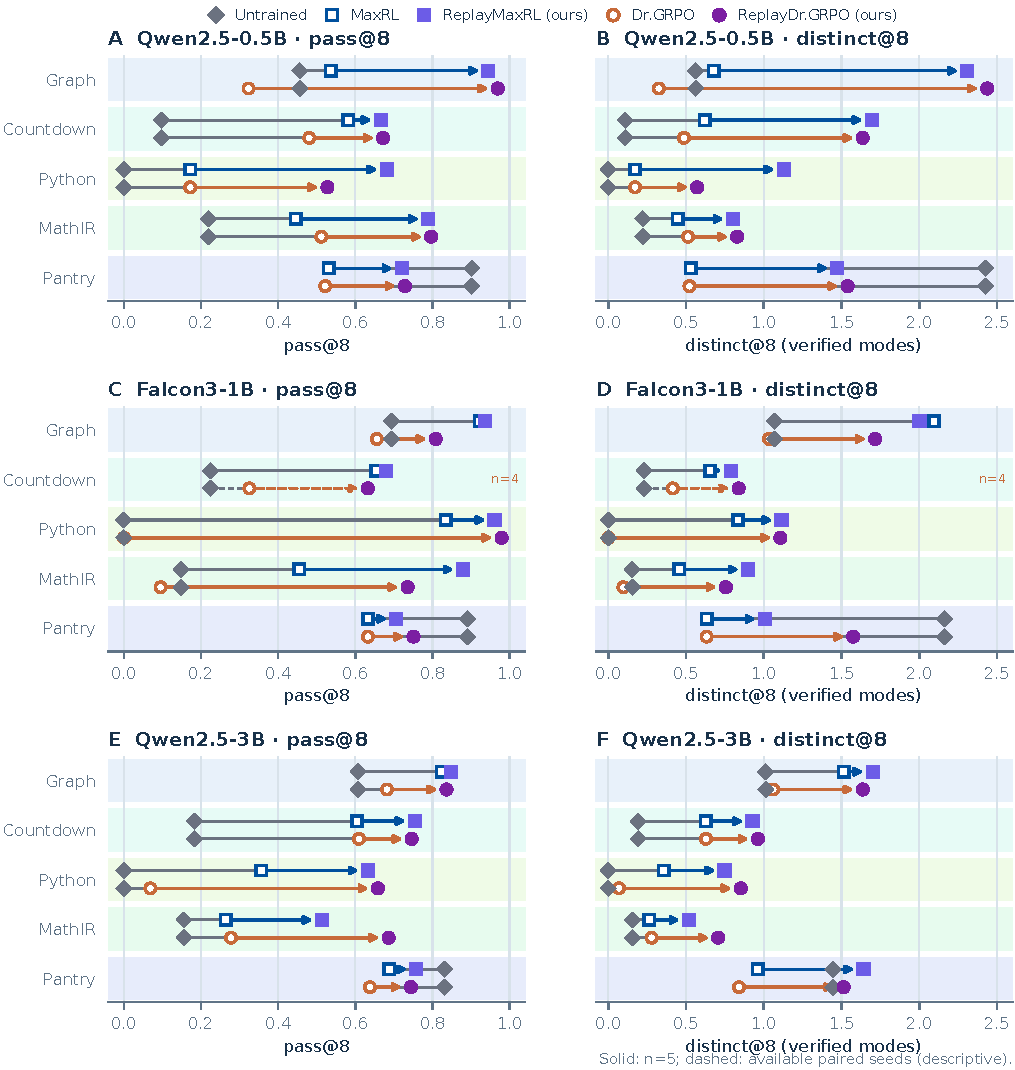
\includegraphics[width=.98\linewidth]
    {figures/e118_scale_extensions_appendix.pdf}
  \caption{\textbf{Replay gains vary by domain and model scale.}
  Final \texttt{pass@8} and \pmd{} at three model scales. Hollow and filled
  markers denote training without and with replay; circles denote Dr.GRPO,
  squares MaxRL, and gray diamonds the model before training. Correctness
  uses five paired seeds except Falcon \texttt{Countdown} Dr.GRPO ($n=4$).
  Diversity averages each arm's eligible seeds separately, requiring at least
  30 eligible prompts per seed. Lines are solid for five control seeds and
  dashed for fewer. Seed counts may differ between arms; estimates below the
  threshold are omitted. Table~\ref{tab:cross-scale-terminal-effects} reports
  paired diversity effects using a 20-prompt threshold. Error bars are omitted.}

  \label{fig:maxrl-factorial-scale-extensions}
\end{figure}


Diversity effects in Fig.~\ref{fig:replay-factorial-effects} and
Table~\ref{tab:cross-scale-terminal-effects} use paired seeds for which
both arms have at least 20 eligible evaluation prompts. The separate-arm
means in Table~\ref{tab:core-terminal-endpoints} and
Fig.~\ref{fig:maxrl-factorial-scale-extensions} instead require 30 eligible
prompts per seed in each arm. Correctness, absolute diversity, and paired
diversity effects can therefore use different seed sets; eligible prompt
subsets can also differ between arms. Diversity-effect intervals use
Student-$t$ with $n-1$ degrees of freedom for $n\ge2$ paired seeds; single-seed
effects have no interval. Correctness and mode-count intervals require five
paired seeds. All intervals are nominal 95\% estimates, without adjustment
for multiple comparisons.

For Qwen2.5-0.5B, Re:Max increases \pmd{} by $+.439$, $+.489$, and
$+.317$ on \texttt{Graph}, \texttt{Countdown}, and \texttt{PantryPlan},
respectively; each five-seed interval excludes zero. Falcon \texttt{Graph}
has a diversity effect of $-.009$ ($[-.034,+.016]$) and a correctness
effect of $+.014$ ($[-.016,+.044]$), both inconclusive. Thus a positive
cross-domain average does not imply improvement in every domain.

For Qwen2.5-3B, the five-seed \pmd{} effects are $+.076$, $+.077$,
$+.058$, $+.006$, and $+.224$ for \texttt{Graph}, \texttt{Countdown},
\texttt{Python}, \texttt{MathIR}, and \texttt{PantryPlan}, respectively.
All diversity intervals exclude zero, although the \texttt{MathIR} effect is
small. Correctness intervals exclude zero for \texttt{Countdown},
\texttt{MathIR}, and \texttt{PantryPlan}, but include zero for \texttt{Graph}
and \texttt{Python}. Across scales, Re:Max exceeds MaxRL in mean \pmd{} in
14 of 15 measurable comparisons; Re:Dr exceeds
Dr.GRPO in 14 of 14. These counts summarize
the signs of the estimated effects, not their statistical significance.

\paragraph{Cross-domain factorial summaries.}
\label{app:factorial-numerical-detail}
Weighting all five domains equally within each paired seed, Re:Max improves
\texttt{pass@8} over MaxRL by $+.307$ at Qwen2.5-0.5B (95\% interval
$[+.208,+.406]$), $+.133$ at Falcon3-1B ($[+.043,+.223]$), and $+.154$
at Qwen2.5-3B ($[+.086,+.222]$). Each comparison uses five seeds. The
corresponding Re:Dr effects are $+.337$, $+.442$, and $+.279$. The Falcon
Dr.GRPO comparison uses four common seeds and has no interval; the other
two use five.

At Qwen2.5-3B, MaxRL and Re:Max have mean correctness $.547$ and $.701$,
and mean \distk{} $.744$ and $1.107$, respectively. Their paired mode-count
difference is $+.363$ ($[+.285,+.441]$). The cross-domain \pmd{} means in
Table~\ref{tab:cross-scale-terminal-effects} use a fixed set of domains
eligible for every contributing seed.

\subsection{Level 1 at Qwen2.5-7B}
\label{app:qwen7b-level1}

We also compare MaxRL and Re:Max at Qwen2.5-7B on Level~1 in
3 domains. The 6 training runs form one
matched treatment--control pair per domain, each trained for
3072 updates with the same prompts, horizon, verifier,
evaluation procedure, and replay schedule as the smaller-scale comparisons.
With one matched seed per domain, these effects are descriptive and have no
confidence intervals.

On \texttt{MathIR}, MaxRL's observed \texttt{pass@8} reaches zero
at update 960 and remains zero at subsequent evaluations.
The final evaluation contains no verified response, so \pmd{} cannot be
estimated. Table~\ref{tab:qwen7b-level1} reports it as undefined rather than
zero. Re:Max, evaluated on the same prompts and seed, reaches
.744 \texttt{pass@8} and .017
\pmd{}. The correctness result remains measurable even though a paired
diversity effect is unavailable.

Where both conditions have measurable diversity, Re:Max increases \pmd{}
by +.298 on \texttt{Graph} and
+.137 on \texttt{Countdown}. These point estimates
exceed the corresponding 3B means, but one seed does not establish a trend
with model scale. Mean \texttt{pass@8} across all 3 domains
is .342 for MaxRL and .789 for Re:Max. Mean
\pmd{} is .028 and .245, respectively, over the
2 domains where both conditions define it. Thus the
correctness mean includes \texttt{MathIR}, while the diversity
mean does not.

\begin{table}[!htbp]
  \centering
  \caption{\textbf{Level-1 correctness and solution diversity at Qwen2.5-7B.}
  Results from 6 runs with 1 matched seed per
  domain after 3072 updates. On \texttt{MathIR},
  MaxRL produces no verified response: its correctness is zero, while its
  \pmd{} and the paired diversity effect are undefined (\texttt{--}).
  Means use 3 domains for correctness and the
  2 jointly eligible domains for diversity. No confidence
  intervals are reported per domain for these single-seed comparisons.}

  \label{tab:qwen7b-level1}
  \small
  \setlength{\tabcolsep}{6pt}
  \begin{tabular}{@{}l*{6}{r}@{}}
    \toprule
    & \multicolumn{2}{c}{\textbf{MaxRL}} & \multicolumn{2}{c}{\textbf{Re:Max}}
      & \multicolumn{2}{c}{\textbf{Re:Max $-$ MaxRL}} \\
    \cmidrule(lr){2-3}\cmidrule(lr){4-5}\cmidrule(lr){6-7}
    \textbf{Domain} & \texttt{pass@8} & \pmd{} & \texttt{pass@8} & \pmd{}
      & \texttt{pass@8} & \pmd{} \\
    \midrule
    % Generated by ops/build_paper_e124_qwen7b_level1.py; do not hand edit.
  \texttt{Countdown} & .631 & .001 & .805 & .138 & +.174 & +.137 \\
  \texttt{Graph} & .396 & .055 & .818 & .353 & +.422 & +.298 \\
  \texttt{MathIR} & .000 & -- & .744 & .017 & +.744 & -- \\
  \midrule
  Mean & .342 & .028 & .789 & .245 & +.447 & +.217 \\
  \bottomrule

  \end{tabular}
\end{table}

\subsection{Results on harder benchmark levels}
\label{app:level2-interim}

\begin{figure}[!htbp]
\centering
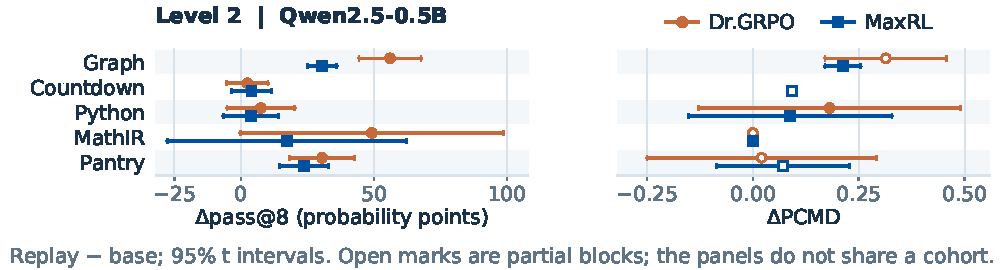
\includegraphics[width=\linewidth]{figures/replay_level2_effects.pdf}
\caption{\textbf{Replay improves Level-2 \texttt{Graph} accuracy and solution diversity.}
Final Re:Dr minus Dr.GRPO (circles) and Re:Max minus MaxRL (squares) effects
for Qwen2.5-0.5B, in percentage points of \texttt{pass@8} and \pmd{} units.
Correctness uses five paired seeds per domain. Diversity requires at least
20 eligible prompts per arm. Re:Dr uses three seeds for \texttt{Graph} and
\texttt{PantryPlan}, four for \texttt{MathIR}, and none for
\texttt{Countdown}; Re:Max uses one for \texttt{Countdown} and four for
\texttt{PantryPlan}. Other comparisons use five. Hollow markers indicate
fewer than five pairs; blanks indicate no eligible pair. Bars show nominal
paired 95\% Student-$t$ intervals for comparisons with at least two seeds.}

  \label{fig:replay-level2-effects}
\end{figure}

Fig.~\ref{fig:level2-admission} compares replay effects across Levels 1--3
using fixed domain sets. Correctness gives equal weight to \texttt{Graph},
\texttt{Countdown}, \texttt{Python}, and \texttt{PantryPlan} within each of
five common training seeds. Diversity first averages eligible seeds within
each arm and domain, then weights \texttt{Graph}, \texttt{MathIR}, and
\texttt{PantryPlan} equally. Its contributing seeds can differ across arms
and levels, so differences between these diversity means are descriptive
and have no intervals. At Level 2, only \texttt{PantryPlan} has sufficient
verified responses before training to estimate diversity; the initial
three-domain diversity mean is therefore undefined.

Each Level-2 method has five final training seeds per domain. The diversity
comparisons in Fig.~\ref{fig:replay-level2-effects} additionally require
eligible prompts in both arms. \texttt{Graph} improves under both objectives:
Re:Max increases \pmd{} by $+.212$ ($[+.170,+.255]$, five seeds), and
Re:Dr by $+.314$ ($[+.170,+.458]$, three seeds). The corresponding
\texttt{Python} effects are $+.088$ and $+.181$, with intervals including
zero; \texttt{MathIR} effects are near zero. \texttt{PantryPlan}
correctness improves by $+.305$ under Re:Dr and $+.237$ under Re:Max,
each measured over five seeds.

Each Level-2 \texttt{MathIR} prompt admits one shortest derivation and four
longer alternatives. Concentration on the shortest route therefore yields
near-zero diversity despite the existence of other valid modes. The levels
also use different held-out problems and can differ in mode-count
distributions and prompt guidance (App.~\ref{app:data-levels}). Cross-level
comparisons consequently do not isolate the causal effect of difficulty.

For each common seed and endpoint $Y$, the replay interaction is
\[
 I=(Y^{\rm Re:Max}-Y^{\rm MaxRL})
    -(Y^{\rm Re:Dr}-Y^{\rm Dr.GRPO}).
\]
A negative interaction means that replay adds less under MaxRL than under
Dr.GRPO; it does not imply that replay harms MaxRL. On Level-2
\texttt{Graph}, MaxRL alone improves \texttt{pass@8} over Dr.GRPO by
$+.233$ ($[+.140,+.325]$), while the replay interaction is $-.256$
($[-.329,-.183]$). Replay improves both objectives, with a smaller
additional benefit under the stronger fresh objective.

\begin{table}[!htbp]
  \centering
  \caption{\textbf{A stronger fresh objective need not increase the additional benefit of replay.}
  Contrasts use five common seeds per domain across all four methods.
  The interaction is
  $(\mathrm{Re:Max}-\mathrm{MaxRL})-(\mathrm{Re:Dr}-\mathrm{Dr.GRPO})$.
  Here $P_8=\texttt{pass@8}$, $D_8=\texttt{distinct@8}$, and $B_8=D_8-P_8$.
  Entries report paired means and nominal 95\% Student-$t$ intervals. Both
  mode-count metrics depend on correctness. The conditional-diversity analysis
  in Fig.~\ref{fig:replay-level2-effects} applies separate eligibility
  requirements, so its seed populations can differ from those in this table.}

\label{tab:level2-factorial-contrasts}
  \scriptsize
  \setlength{\tabcolsep}{3pt}
  \resizebox{\linewidth}{!}{%
  \begin{tabular}{@{}lclrrr@{}}
    \toprule
    \textbf{Domain} & $n$ & \textbf{Contrast} &
    $\Delta P_8$ & $\Delta D_8$ & $\Delta B_8$ \\
    \midrule
    % Domain & paired n & contrast & delta pass@8 & delta distinct@8 & delta extra modes
Graph & 5 & MaxRL $-$ Dr.GRPO & $+.233\;[+.140,+.325]$ & $+.322\;[+.162,+.482]$ & $+.089\;[+.019,+.159]$ \\
Graph & 5 & Re:Max $-$ Re:Dr & $-.023\;[-.062,+.016]$ & $-.029\;[-.198,+.140]$ & $-.006\;[-.142,+.130]$ \\
Graph & 5 & Replay $\times$ MaxRL interaction & $-.256\;[-.329,-.183]$ & $-.351\;[-.446,-.255]$ & $-.095\;[-.186,-.003]$ \\
Countdown & 5 & MaxRL $-$ Dr.GRPO & $-.014\;[-.073,+.045]$ & $-.014\;[-.073,+.045]$ & $+.000\;[+.000,+.000]$ \\
Countdown & 5 & Re:Max $-$ Re:Dr & $+.002\;[-.008,+.012]$ & $-.002\;[-.047,+.044]$ & $-.004\;[-.042,+.035]$ \\
Countdown & 5 & Replay $\times$ MaxRL interaction & $+.016\;[-.047,+.078]$ & $+.012\;[-.068,+.092]$ & $-.004\;[-.042,+.035]$ \\
Python & 5 & MaxRL $-$ Dr.GRPO & $+.000\;[+.000,+.000]$ & $+.000\;[+.000,+.000]$ & $+.000\;[+.000,+.000]$ \\
Python & 5 & Re:Max $-$ Re:Dr & $-.037\;[-.232,+.157]$ & $-.188\;[-.988,+.613]$ & $-.150\;[-1.014,+.713]$ \\
Python & 5 & Replay $\times$ MaxRL interaction & $-.037\;[-.232,+.157]$ & $-.188\;[-.988,+.613]$ & $-.150\;[-1.014,+.713]$ \\
MathIR & 5 & MaxRL $-$ Dr.GRPO & $+.283\;[-.193,+.759]$ & $+.283\;[-.193,+.759]$ & $+.000\;[+.000,+.000]$ \\
MathIR & 5 & Re:Max $-$ Re:Dr & $-.036\;[-.158,+.085]$ & $-.035\;[-.158,+.088]$ & $+.002\;[-.003,+.006]$ \\
MathIR & 5 & Replay $\times$ MaxRL interaction & $-.320\;[-.864,+.225]$ & $-.318\;[-.860,+.224]$ & $+.002\;[-.003,+.006]$ \\
PantryPlan & 5 & MaxRL $-$ Dr.GRPO & $+.019\;[-.067,+.105]$ & $+.019\;[-.081,+.119]$ & $+.000\;[-.021,+.021]$ \\
PantryPlan & 5 & Re:Max $-$ Re:Dr & $-.049\;[-.113,+.014]$ & $-.061\;[-.249,+.128]$ & $-.012\;[-.145,+.122]$ \\
PantryPlan & 5 & Replay $\times$ MaxRL interaction & $-.068\;[-.168,+.032]$ & $-.080\;[-.279,+.119]$ & $-.012\;[-.134,+.110]$ \\
    \bottomrule

  \end{tabular}}
\end{table}


\paragraph{Level-2 \texttt{Graph} results.}
\label{app:levels-numerical-detail}
Before training, Qwen2.5-0.5B \texttt{Graph} \texttt{pass@8} is $.438$
on the Level-1 development split and $.148$ on Level 2. After eight Level-2
training passes, Dr.GRPO and MaxRL reach $.202$ and $.434$, compared
with $.763$ and $.739$ for Re:Dr and Re:Max. The paired correctness gains
are $+.561$ and $+.305$, with 95\% Student-$t$ intervals $[+.445,+.677]$
and $[+.250,+.360]$ over five seeds each. The lowest replay accuracy
($.711$) exceeds the highest accuracy without replay ($.477$). Replay adds
$1.019$ and $.668$ distinct verified modes for the two objectives,
respectively, yielding \texttt{distinct@8} of $1.243$ and $1.214$.

For the three eligible Dr.GRPO seed pairs, \pmd{} rises from $.039$ to
$.353$; for the five MaxRL pairs, it rises from $.112$ to $.325$.
Expressed on the effective-mode scale, these changes are $1.04$ to $1.55$
and $1.13$ to $1.48$, corresponding to ratios of $1.49$ and $1.32$.
Relative increases in \pmd{} are unstable near a zero baseline, so we
report absolute changes instead. The joint improvements in correctness and
diversity do not establish that greater diversity causes better correctness.

\subsection{Accuracy and verified modes throughout training}
\label{app:factorial-training-curves}

Figs.~\ref{fig:factorial-training-accuracy}--\ref{fig:level2-training-pmd}
show correctness and diversity throughout training, using four groups of
eight responses to each of 128 held-out prompts. Lines show seed means;
bands show the range across seeds, rather than confidence intervals. A seed
contributes to conditional diversity only when at least five prompts have
two or more correct responses. The contributing seeds and prompts can
therefore change across methods and checkpoints.

\begin{figure}[!htbp]
  \centering
  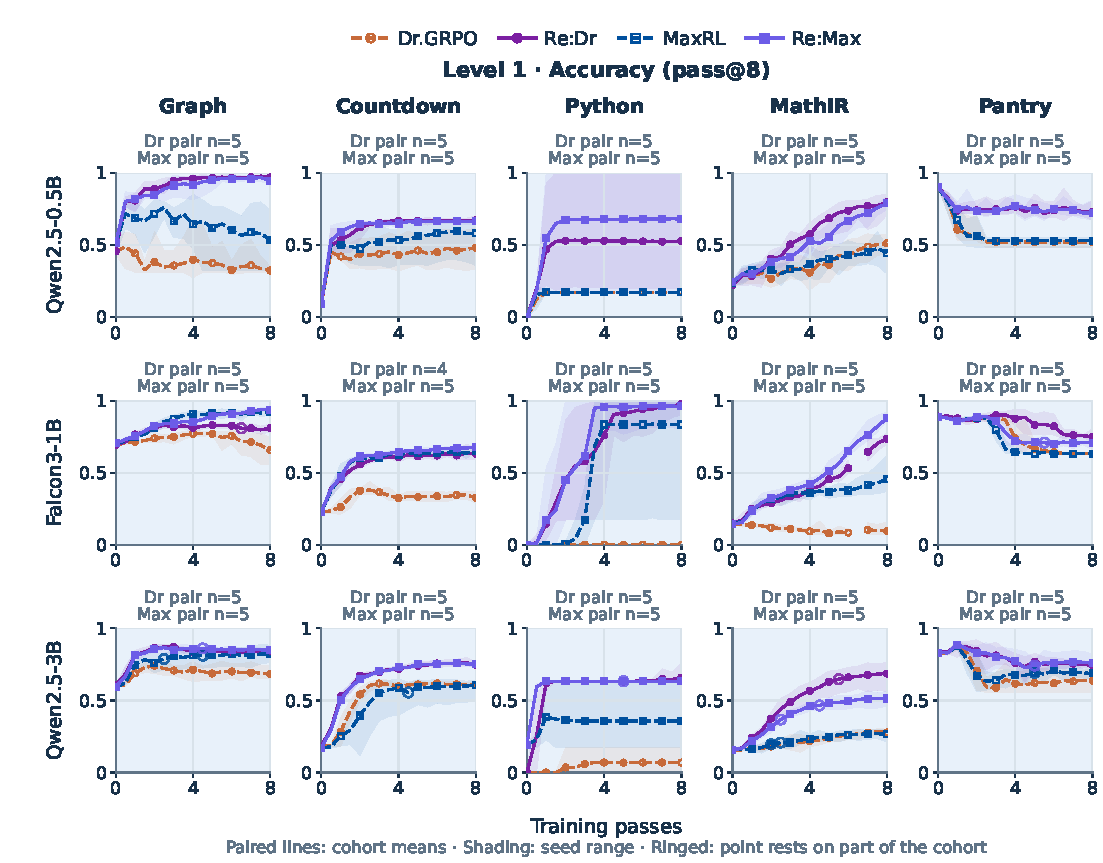
\includegraphics[width=\linewidth]{figures/factorial_training_curves_pass8.pdf}
  \caption{\textbf{Replay improves final accuracy across model scales.}
  \texttt{pass@8} over eight training passes for Dr.GRPO, Re:Dr, MaxRL, and
  Re:Max. Rows show Qwen2.5-0.5B, Falcon3-1B, and Qwen2.5-3B; columns show
  domains. Panel labels give the numbers of paired seeds at the final
  checkpoint. Lines show seed means and bands show seed ranges, rather than
  confidence intervals. Ringed points use fewer seeds than the final comparison.}

  \label{fig:factorial-training-accuracy}
\end{figure}

\begin{figure}[!htbp]
  \centering
  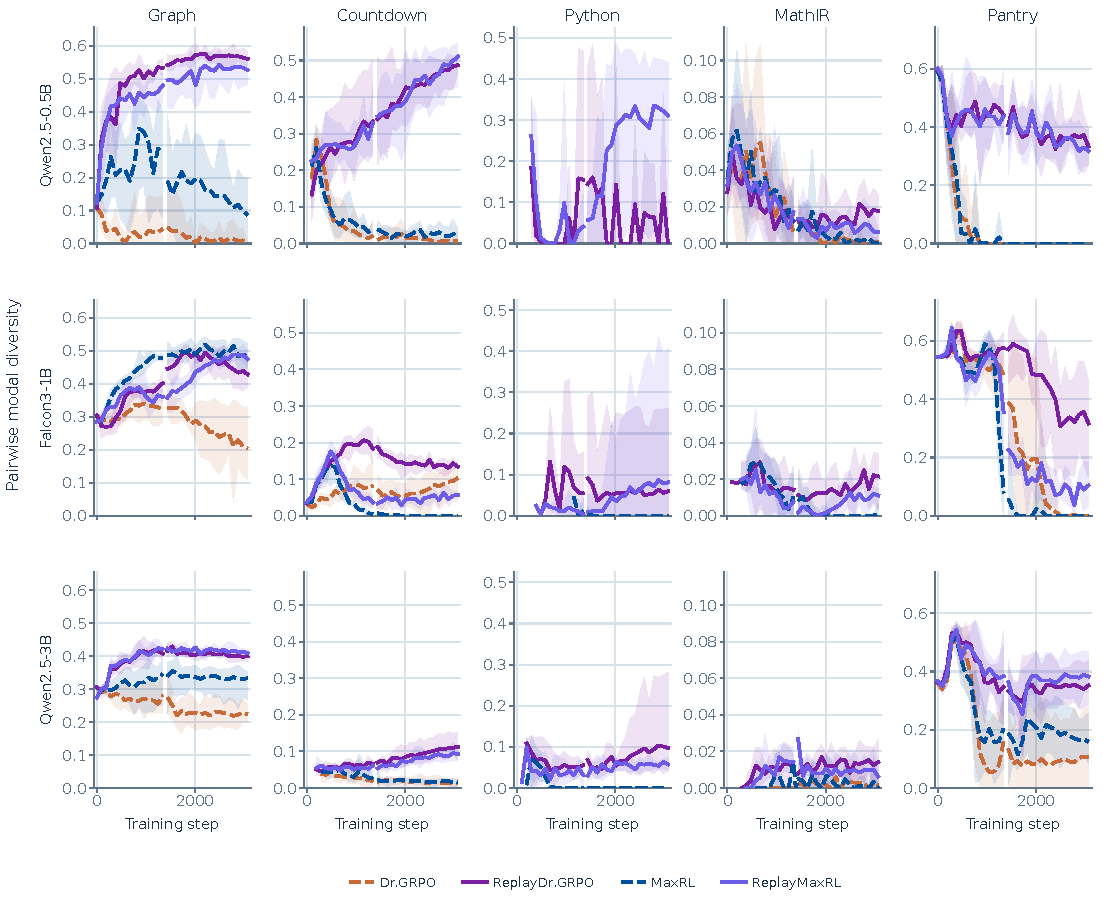
\includegraphics[width=\linewidth]{figures/factorial_training_curves_pmd.pdf}
  \caption{\textbf{Replay limits the loss of \texttt{PantryPlan} solution diversity at every scale.}
\pmd{} throughout training, with model rows and method colours as in
Fig.~\ref{fig:factorial-training-accuracy}. Both fresh objectives reach zero
terminal \texttt{PantryPlan} diversity at 0.5B and 1B, whereas both replay variants
retain multiple solution modes. Lines average one to five eligible seeds
per checkpoint; bands show seed ranges and are absent for a single seed.
A seed contributes when at least five prompts yield at least two correct responses.
Fine dotted segments use fewer seeds, so changes can reflect sample
composition. Gaps indicate undefined estimates. Vertical scales are shared
within each domain.}
  \label{fig:factorial-training-modes}
\end{figure}

\begin{figure}[!htbp]
  \centering
  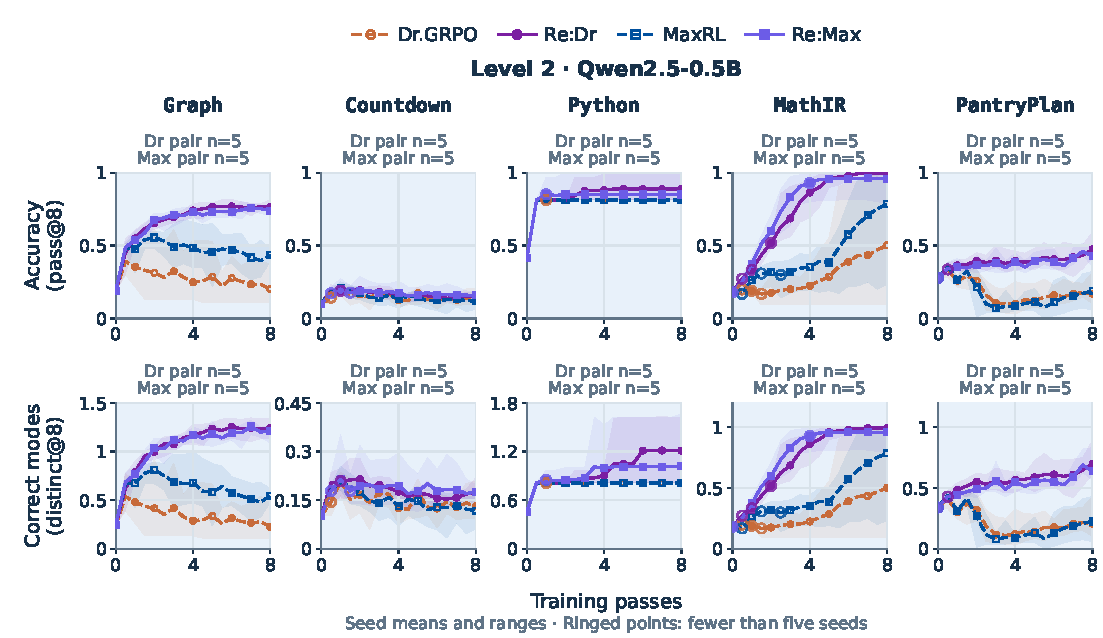
\includegraphics[width=\linewidth]{figures/level2_factorial_training_curves.pdf}
  \caption{\textbf{Replay improves final accuracy and verified-mode counts at Level~2.}
Qwen2.5-0.5B trajectories for Dr.GRPO, Re:Dr, MaxRL, and Re:Max across five
domains. Rows show \texttt{pass@8} and \distk{}; the latter depends on both
correctness and solution diversity. Each objective pair has five matched
seeds at the terminal checkpoint. Lines show seed means and bands show
seed ranges. Ringed points use fewer than five seeds; Fig.~\ref{fig:level2-training-pmd}
reports success-conditional diversity.}
  \label{fig:level2-training-curves}
\end{figure}

\begin{figure}[!htbp]
  \centering
  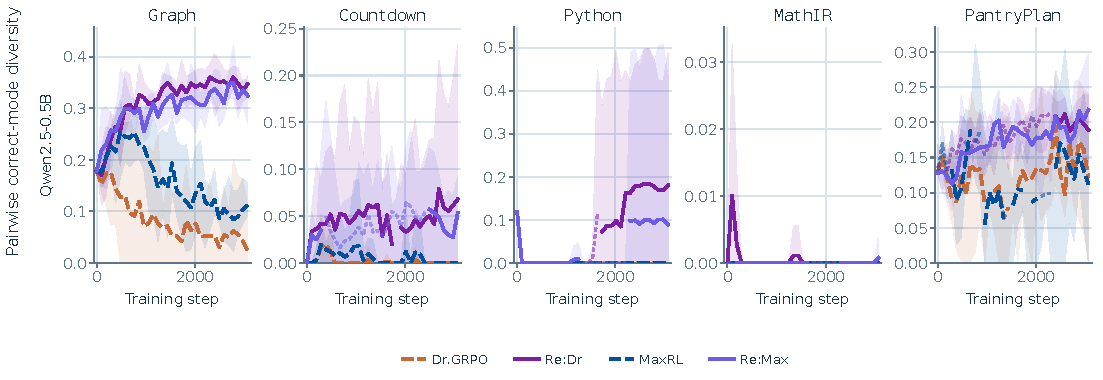
\includegraphics[width=\linewidth]{figures/level2_training_curves_pmd.pdf}
  \caption{\textbf{Replay preserves greater solution diversity on Level-2 \texttt{Graph}.}
\pmd{} during Qwen2.5-0.5B training for the four primary methods. At the
terminal checkpoint, Re:Dr and Re:Max reach $.346$ and $.325$, compared with
$.023$ for Dr.GRPO and $.112$ for MaxRL. \texttt{MathIR} remains near zero under all
four methods. Lines average eligible seeds and bands show seed ranges.
Each seed requires at least five prompts with at least two correct responses.
Fine dotted segments indicate fewer contributing seeds, and gaps indicate that the estimate is undefined.}
  \label{fig:level2-training-pmd}
\end{figure}


\subsection{Supporting comparators}
\label{app:ucpo-progress}

GRPO normalizes rewards within each group; UCPO redistributes the advantage
among fresh on-policy responses; sparse RLEP-Dr reuses verified successes
without uniform weighting by canonical key. We evaluate GRPO in 75 training
runs across three model scales. UCPO and RLEP-Dr cover the two smaller
scales, with 50 and 47 runs, respectively. RLEP-Dr uses two seeds for Falcon
\texttt{Python} and five elsewhere. Fixed Semantic-MaxEnt adds a
frequency-based bonus to fresh responses (App.~\ref{app:semantic-maxent}).
Its four-method factorial covers ten model--domain combinations at the two
smaller scales, with five common seeds except Falcon \texttt{Countdown}
($n=4$). The 3B comparison uses one seed to evaluate adding the bonus to
replay (App.~\ref{app:semantic-current-factorial}).

For GRPO, UCPO, and RLEP-Dr, the diversity contrasts in this subsection
average per-prompt differences over prompts with at least two correct
responses in both arms. Each seed must have at least 30 such jointly
eligible prompts. Table~\ref{tab:direct-comparator-matrix} instead uses
separate 20-prompt thresholds for each arm. On Qwen2.5-0.5B \texttt{Graph},
one UCPO seed and four RLEP-Dr seeds meet the joint criterion; no
\texttt{Python} comparison meets it at any scale.

For Qwen2.5-0.5B, UCPO improves \texttt{Countdown} \texttt{pass@8} by
$+.133$ ($[+.005,+.262]$), while its \pmd{} effect is inconclusive:
$+.002$ ($[-.018,+.023]$). Its \texttt{MathIR} effects are also
inconclusive. RLEP-Dr improves \texttt{MathIR} correctness by $+.126$
($[+.030,+.222]$), with zero measured diversity change; its
\texttt{Countdown} and Falcon \texttt{PantryPlan} effects are inconclusive.
Across GRPO, UCPO, and RLEP-Dr, seven of 34 five-seed correctness intervals
lie above zero. None of the 19 five-seed diversity intervals lies above zero; one lies
below zero, for Falcon \texttt{Countdown} GRPO: $-.105$
($[-.147,-.063]$). At Qwen2.5-3B, all five GRPO correctness intervals and
the three available diversity intervals include zero. These are nominal
paired 95\% Student-$t$ intervals over training seeds.

The uniform versus frequency-weighted replay comparison uses five paired
seeds in each of nine model--domain combinations: all five Qwen2.5-0.5B
domains, plus \texttt{Graph} and \texttt{PantryPlan} at both larger scales.
Changing only the within-buffer weights increases extra verified modes by
$+.318$ per prompt in the Qwen2.5-0.5B average ($[+.272,+.358]$,
paired-seed bootstrap). The correctness effect is inconclusive at $+.010$
($[-.119,+.139]$). This result supports a benefit from uniform weighting
beyond reusing successful responses in proportion to their frequency,
although extra-mode counts still depend on correctness
(App.~\ref{app:frequency-replay-progress}).

RLEP-Dr's offline response pool uses temperature $.7$ and top-$p=.95$;
evaluation uses temperature 1 and top-$p=1$. Its offline data collection
also differs from the online construction of prompt-specific verified replay
buffers, and the next paragraph measures what that difference puts in the pool.

\paragraph{What RLEP-Dr replays.}
\phantomsection\label{app:rlep-pool}
RLEP's protocol harvests its experience pool from a policy that RL has
already trained \citep{zhang2025rlep}: the seed policy samples 64 candidates
per prompt at temperature $.7$ and top-$p=.95$, verified answers are kept, and
a prompt enters the pool only with at least two of them. Here the seed policy
is the paired terminal Dr.GRPO control, so the pool is a sample from the
collapsed endpoint that Sec.~\ref{sec:results-collapse} measures.
Table~\ref{tab:rlep-pool-composition} reads the frozen pools and the learner
telemetry of every RLEP-Dr cell. At Qwen2.5-0.5B,
43\%--79\% of the 384 training prompts hold
no verified trajectory and never receive a replay row. Of the
4393 eligible prompts pooled over all 25
cells, all but 17 hold a single canonical key among
their verified trajectories, and none holds more than 2, so a
two-row replay draw is two copies of one mode with probability at least
.99 in every domain.
Falcon3-1B pools are slightly wider on \texttt{Graph} and \texttt{Countdown},
up to 1.40 keys per eligible prompt, and a same-mode pair
remains the draw with probability
.89--1.00. The online Re:Dr buffer on the
same prompts and seeds holds 2.6--6.9 modes on average
in the three domains where modes are plentiful. RLEP-Dr's replay is therefore
single-mode replay of the control's own endpoint, applied on
21\%--57\% of updates, and its \pmd{} beside the
control is the expected outcome rather than a discrepancy with Re:Dr: no
update rule rehearses a second mode from a pool that holds one.

The two update rules are closer than their descriptions suggest. RLEP's
replay row enters the policy gradient with advantage $1-\bar r$, where
$\bar r$ is the mean reward of the mixed group, so it is a positive-coefficient
log-likelihood term on a stored success, as Re:Dr's replay term is. The
difference is that RLEP's coefficient shrinks toward zero as the prompt is
solved, with a realized mean of .03--.38 across domains
at 0.5B, whereas Re:Dr's is fixed. Whether a likelihood term on a single
stored success can produce breadth is tested directly by the capacity-one arm
of App.~\ref{app:mode-agnostic-replay}, which applies exactly such a term to
one success captured online at first discovery and recovers 58\% of
the Re:Dr effect. What separates the two replay families is thus not the loss
but the buffer: what it stores, from which policy, and from when.

\begin{table}[H]
  \centering
  \caption{\textbf{RLEP-Dr's pools hold one mode per prompt.} Composition of
  the frozen RLEP experience pools and the realized replay dose, averaged over
  seeds. \emph{none} is the share of the 384 training prompts with no verified
  trajectory; \emph{eligible} the share with at least two; \emph{keys} the mean
  number of canonical modes among an eligible prompt's verified trajectories;
  $P(\text{same})$ the probability that a two-row replay draw repeats one
  mode; \emph{updates} the share of optimizer updates that mixed in replay
  rows; $A_{\text{replay}}$ the mean replay advantage $1-\bar r$ on those
  updates. The last column is the mean number of modes in the Re:Dr buffer
  over the within-cohort cells on the same prompts and seeds
  (Tab.~\ref{tab:matched-redr}).}
  \label{tab:rlep-pool-composition}
  \small
  \setlength{\tabcolsep}{5pt}
  \begin{tabular}{@{}lrrrrrrrr@{}}
    \toprule
    \textbf{Domain} & $n$ & \textbf{none} & \textbf{eligible} & \textbf{keys}
      & $P(\text{same})$ & \textbf{updates} & $A_{\text{replay}}$
      & \textbf{Re:Dr modes} \\
    \midrule
    % Generated by ops/build_paper_rlep_pool_composition.py; do not hand edit.
  \multicolumn{9}{@{}l}{\textit{Qwen2.5-0.5B}} \\
  \texttt{Graph} & 5 & 64\% & 36\% & 1.00 & 1.00 & 36\% & .19 & 3.77 \\
  \texttt{Countdown} & 5 & 43\% & 57\% & 1.02 & .99 & 57\% & .11 & 2.56 \\
  \texttt{Python} & 5 & 79\% & 21\% & 1.00 & 1.00 & 21\% & .03 & 1.20 \\
  \texttt{MathIR} & 5 & 43\% & 57\% & 1.00 & 1.00 & 57\% & .38 & 1.15 \\
  \texttt{PantryPlan} & 5 & 43\% & 57\% & 1.00 & 1.00 & 57\% & .03 & 6.88 \\
  \multicolumn{9}{@{}l}{\textit{Falcon3-1B}} \\
  \texttt{Graph} & 5 & 44\% & 56\% & 1.40 & .89 & 56\% & .41 & \textemdash{} \\
  \texttt{Countdown} & 5 & 56\% & 44\% & 1.17 & .95 & 44\% & .24 & \textemdash{} \\
  \texttt{Python} & 2 & 90\% & 10\% & 1.01 & 1.00 & 10\% & .50 & \textemdash{} \\
  \texttt{MathIR} & 5 & 91\% & 9\% & 1.01 & 1.00 & 9\% & .30 & \textemdash{} \\
  \texttt{PantryPlan} & 5 & 41\% & 59\% & 1.00 & 1.00 & 59\% & .09 & \textemdash{} \\
  \bottomrule

  \end{tabular}
\end{table}

\paragraph{Comparator settings.}
\phantomsection\label{app:comparator-settings}
Each comparator shares the non-objective settings of its paired control
(Table~\ref{tab:run-contract}). UCPO uses the published default
$\omega=.2$, and RLEP-Dr uses the published combination of 16 fresh and
2 replay responses. GAPO has no free coefficient; its reward is affinely
mapped to the control's unit range because Dr.GRPO does not normalize by
the group standard deviation. SetPO uses $\lambda=1.0$, giving a diversity
term approximately 5.3\% of the task advantage; its paper provides no
coefficient for the 0.5B verifier-reward setting. Semantic-MaxEnt uses
$\eta=.10$ and $\kappa=5$. Replay uses $\lambda_{\mathrm{replay}}=.10$
and capacity $M=16$, equal to the rollout group size. These settings are
not tuned to \mb{} outcomes, and no method receives a learning-rate sweep.
The results therefore compare the methods at the stated settings;
hyperparameter tuning could improve correctness or diversity.

\paragraph{Interpreting zero diversity.}
In Table~\ref{tab:direct-comparator-matrix}, an em-dash denotes an undefined
paired difference. An exact $.000$ instead denotes a measured zero, with
identical values for both methods in every eligible seed. The
\texttt{Python} \pmd{} column contains measured zeros because, for each
eligible prompt, both methods' verified responses share a single execution
key. High correctness can coexist with this concentration: four of the five
SetPO \texttt{Python} seeds reach \texttt{pass@8} $1.000$ and terminal
\pmd{} $.000$. Every held-out prompt has at least one correct response,
but the verified responses for each prompt use a single mode. Per-response
correctness also increases in all 15 control comparisons
(App.~\ref{app:control-learning-audit}).

\begin{figure}[!htbp]
  \centering
  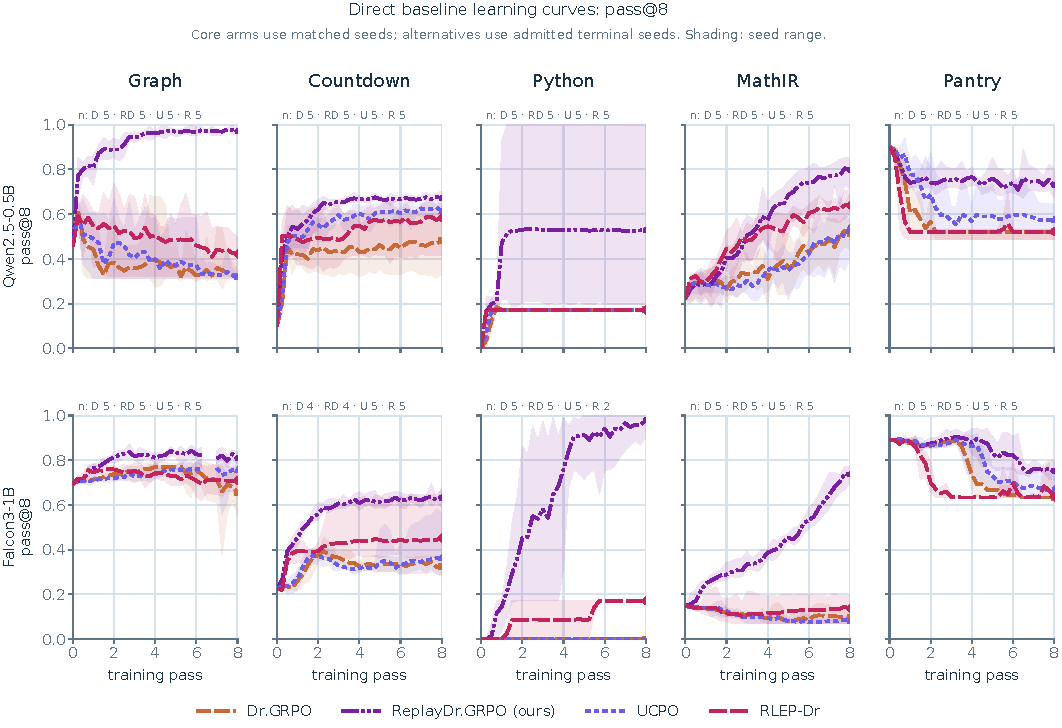
\includegraphics[width=\linewidth]{figures/direct_baseline_learning_curves_pass8.pdf}
  \caption{\textbf{Re:Dr has the highest terminal mean accuracy in every
  displayed comparison.} \texttt{pass@8} during Level-1 training for Dr.GRPO,
  Re:Dr, UCPO, and sparse RLEP-Dr. Rows show Qwen2.5-0.5B and Falcon3-1B;
  columns show the five domains. Lines show seed means and bands show seed
  ranges; gaps indicate unavailable estimates. Dr.GRPO and Re:Dr use paired
  seeds. Comparisons use five seeds except Falcon \texttt{Countdown}
  Dr.GRPO/Re:Dr ($n=4$) and Falcon \texttt{Python} RLEP-Dr ($n=2$), as indicated in the panels.}
  \label{fig:direct-baseline-accuracy-curves}
\end{figure}


\subsection{Diversity-preserving comparators}
\label{app:diversity-comparators}

GAPO~\citep{anschel2025groupaware} and SetPO~\citep{li2026setpo} target
output diversity within the fresh rollout group. Both are evaluated on
Level-1 Qwen2.5-0.5B across five domains and five seeds. GAPO assigns
verifier-positive rollouts the reward $[1-(f_i-1/L)+1]/2$, with zero for
failures, where $f_i$ is the key's frequency among the group's verified
rollouts and $L$ is the prompt's certified number of valid modes.
SetPO augments each rollout's advantage by its marginal contribution to
kernelized set diversity, measured by removing that rollout from the group,
with coefficient $\lambda=1$. It computes similarities using a fixed
\texttt{all-MiniLM-L6-v2} sentence encoder, mean pooling, and cosine
similarity clamped to $[0,1]$. Encoding the responses adds computation.

GAPO increases \pmd{} on \texttt{Countdown} ($+.340$, $[+.112,+.567]$) and \texttt{PantryPlan}
($+.653$, $[+.610,+.696]$), while its \texttt{Python} effect is near zero
with an interval spanning zero. \texttt{Python} has more valid modes than the
sixteen-rollout group can represent on 95\% of training prompts, with up to 3,600
modes. This limits within-group coverage but does not prevent a policy from
assigning mass across the full support. \texttt{MathIR} effects are small across
methods; the largest is Re:Dr's $+.017$ ($[+.003,+.031]$).
SetPO increases \pmd{} on \texttt{PantryPlan} ($+.266$, $[+.177,+.356]$); its other
four domain intervals include zero. Five-domain mean effects are $+.225$
for GAPO, $+.066$ for SetPO, and $+.320$ for Re:Max, although GAPO's
\texttt{PantryPlan} effect is larger than Re:Max's. The effective number
of modes, $\neff$, on \texttt{PantryPlan} is $2.88$ for GAPO and $1.36$
for SetPO, compared with $1.00$ for their shared control. SetPO also raises
\texttt{Python} \texttt{pass@8} from $.338$ to $.834$, a relative increase
of $147\%$. Relative changes in \pmd{} are undefined for \texttt{PantryPlan}
and \texttt{Python} because the control has $\pmd=.000$. GAPO adjusts
rewards using frequencies within the fresh rollout group, whereas replay
balances the likelihood term across verified modes accumulated in the buffer.

GAPO and SetPO share a Dr.GRPO control with matching hardware and
nonoverlapping evaluation draws. Its terminal \pmd{} differs from the
Dr.GRPO control used in the main replay comparison by a mean of $+.003$
over twenty paired comparisons, ranging from $-.014$ to $+.034$. These
observed differences are small relative to the five-domain effects above,
but do not establish equivalence between the controls.

\subsection{Measured KL tradeoffs and replay occupancy}
\label{app:kl-measured}

Table~\ref{tab:reference-kl-measured} compares terminal \pmd{} at
Qwen2.5-0.5B, Level~1, after $3{,}072$ updates. Dr.GRPO with reference KL
uses 6 coefficients, $\beta\in\{0.001, 0.01, 0.04, 0.1, 0.2, 0.3\}$, across
5 domains. These arms use the zero-replay-derivative control
configuration with a nonzero KL coefficient and the initial policy as the
reference. The comparisons match optimizer updates and fresh-rollout
budgets. They do not equalize total computation: reference-policy evaluation
and replay processing incur different costs, and the control does not spend
those costs on additional effective updates or fresh rollouts.

\begin{figure}[t]
  \centering
  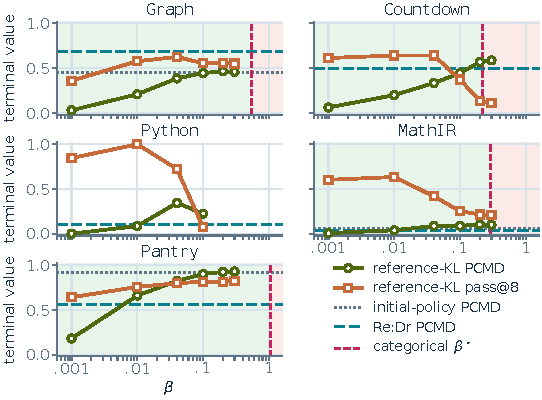
\includegraphics[width=0.78\linewidth]{figures/reference_kl_knee.pdf}
  \caption{\textbf{KL coefficient effects vary by domain.}
  Circles show terminal \pmd{} and squares show \texttt{pass@8} for
  Qwen2.5-0.5B at Level~1; lines connect seed means without uncertainty
  bands. Horizontal rules mark the initial policy's reportable \pmd{}
  (dotted) and Re:Dr's terminal \pmd{} (dashed). Vertical rules mark the
  categorical plug-in threshold $\beta^\star$; green and red indicate
  stationary single-draw correctness above and below one half under that
  calculation. This threshold does not predict the location of the observed
  \texttt{pass@8} knee.}
  \label{fig:reference-kl-knee}
\end{figure}

\paragraph{Initial concentration and coefficient dependence.}
Dr.GRPO without KL reaches \pmd{} at or below $.004$ in all five domains.
MaxRL without replay reaches $.148$ in \texttt{Graph} and at or below $.022$
elsewhere. These low values are consistent with concentration, but the
neural runs do not satisfy the independent-logit assumptions of
Proposition~\ref{thm:grpo-collapse}.
KL produces larger conditional-diversity estimates at several coefficients
in every domain. The response is not uniformly monotone: \texttt{Graph} changes
from $.465$ to $.458$ and \texttt{MathIR} from $.103$ to $.099$ between
$\beta=.2$ and $.3$, while \texttt{Python} changes from $.344$ to $.225$ between
$\beta=.04$ and $.1$.
These are comparisons of point estimates, without a seed-level uncertainty
analysis for their differences.

\begin{table}[t]
  \centering
  \caption{\textbf{KL and replay have different domain-level tradeoffs.}
  Terminal \pmd{} seed means for Qwen2.5-0.5B, Level~1. Superscripts give
  counts below five seeds; dashes indicate unavailable cells. The four
  zero-KL arms use 32 disjoint evaluation streams; KL arms use their own
  disjoint draws with the same estimator. Reference summaries are
  initial-policy \pmd{} and $1-1/\bar k$ for each replay arm, where $\bar k$
  is the mean number of keys replayed per measured update. These do not bound
  neural diversity. The final column computes categorical $\beta^\star$
  from mean initial single-draw correctness.}
  \label{tab:reference-kl-measured}
  \scriptsize
  \setlength{\tabcolsep}{2.5pt}
  \begin{tabular}{@{}lrrrrrrrrrrrrrr@{}}
    \toprule
    & \multicolumn{2}{c}{\textbf{without replay}}
      & \multicolumn{6}{c}{\textbf{$+$ reference KL, by $\beta$}}
      & \multicolumn{2}{c}{\textbf{$+$ replay}}
      & \multicolumn{3}{c}{\textbf{reference summaries}} & \\
    \cmidrule(lr){2-3}\cmidrule(lr){4-9}\cmidrule(lr){10-11}\cmidrule(lr){12-14}
    \textbf{Domain} & Dr.GRPO & MaxRL
      & $.001$ & $.01$ & $.04$ & $.1$ & $.2$ & $.3$
      & \textbf{Re:Dr} & \textbf{Re:Max}
      & Initial & Re:Dr & Re:Max & $\beta^\star$ \\
    \midrule
    % Generated by ops/build_reference_kl_comparison.py; do not hand edit.
  \texttt{Graph}  &  0.003  &  0.148  &  0.029  &  0.207  &  0.385  &  0.444  &  0.465  &  0.458  &  0.686  &  0.625  &  0.45  &  0.75  &  0.70  &  0.55 \\
  \texttt{Countdown}  &  0.004  &  0.022  &  0.060  &  0.198  &  0.333  &  0.444  &  0.568  &  0.587  &  0.497  &  0.531  &  ---  &  0.56  &  0.52  &  0.22 \\
  \texttt{Python}  &  0.000  &  0.000  &  0.000  &  0.086  &  0.344  &  0.225$^{3}$  &  ---  &  ---  &  0.099  &  0.239  &  ---  &  0.15  &  0.42  &  --- \\
  \texttt{MathIR}  &  0.003  &  0.008  &  0.007  &  0.038  &  0.086  &  0.088  &  0.103  &  0.099  &  0.039  &  0.018  &  0.06  &  0.15  &  0.12  &  0.29 \\
  \texttt{Pantry}  &  0.000  &  0.000  &  0.180  &  0.660  &  0.824  &  0.901  &  0.925  &  0.931  &  0.557  &  0.556  &  0.91  &  0.85  &  0.85  &  1.05 \\
  \bottomrule

  \end{tabular}
\end{table}

\paragraph{Stationary predictions and measured checkpoints.}
Proposition~\ref{prop:kl-stationary} identifies the categorical interior
stationary conditional as $q^\star=\mu|_{\mathcal C}$, independently of
$\beta$. It does not bound transient diversity or establish that a finite
neural checkpoint reaches this conditional. The measured \pmd{} varies
with $\beta$ and can exceed the initial estimate: at $\beta=.2$, \texttt{Graph}
reaches $.465$ against $.454$ initially, \texttt{MathIR} $.103$ against $.061$,
and \texttt{Pantry} $.925$ against $.913$. These estimates also condition on each
policy's own verified responses, rather than on a common set of solved
prompts.

For a fixed prompt with $0<\mu(\mathcal C)<1/2$, the Dr.GRPO formula gives
\[
  \beta^\star=\frac{(G-1)/G}{-\operatorname{logit}\mu(\mathcal C)},
  \qquad P^\star(\beta^\star)=\tfrac12.
\]
The displayed values substitute each domain's mean initial correctness
and $G=16$, giving $0.22$--$1.05$.
This aggregation is descriptive: substituting a mean into the nonlinear
stationary formula does not give the mean of its promptwise predictions.
Moreover, $P^\star$ is single-draw correctness, whereas the plotted
\texttt{pass@8} measures success within eight responses. Declines in that
metric already occur below the displayed threshold: \texttt{MathIR} falls from
$.634$ at $\beta=.01$ to $.418$ at $.04$, well below its
$\beta^\star\simeq.29$. \texttt{Countdown} similarly falls from $.642$ at $.04$
to $.372$ at $.1$, below $.22$. The thresholds therefore do not locate
the measured knees. \texttt{Python} has zero observed initial successes, so no
finite plug-in threshold or reportable initial \pmd{} is shown; this
does not establish zero population correctness.

Finite training, shared parameters, prompt sampling, and the adaptive
optimizer can all separate the measured neural trajectory from the
categorical stationary calculation. The comparison does not identify their
individual effects. The boundary-force identities and the two-mode
$\Theta(1/[s\log(1/s)])$ versus $\Theta(\log(1/s))$ recovery result
characterize their stated categorical models, not measured neural recovery
rates.

\paragraph{What buffer occupancy measures.}
For a nonempty fixed uniform categorical buffer with $k$ keys, the limiting
diversity is $1-1/k$. Across such buffers,
$\E[1-1/k]\le1-1/\E[k]$ by Jensen's inequality. The table instead uses
$\bar k$, the number of keys replayed per measured update, averaged within
runs and then across seeds. Buffers change during training, and updates
without replay can contribute zero keys. Thus $1-1/\bar k$ is a
descriptive transform of training occupancy, not an estimate of the
nonempty fixed-buffer expectation in that inequality. Neither quantity
bounds held-out neural \pmd{}.

\texttt{Python} illustrates a possible discovery difference. Re:Max averages
$1.73$ replayed keys per update against Re:Dr's $1.18$, while terminal
\pmd{} is $.239$ versus $.099$. Corollary~\ref{cor:maxrl-starvation}
provides a categorical motivation for stronger fresh learning when
correctness is scarce, but these measurements do not isolate discovery
from prompt weighting, sampling, or optimization. Occupancy also does not
order all outcomes: in \texttt{Countdown}, Re:Max has fewer replayed keys per
update ($2.10$ versus $2.28$) but higher \pmd{} ($.531$ versus $.497$).
In \texttt{Pantry} both arms average about $6.7$ keys and reach about $.557$ \pmd{}.
The capacity of 16 keys would allow a uniform fixed-buffer value of
$1-1/16=.9375$; the occupancy summary near $.85$ is not that capacity
limit and does not prove why KL performs better there.

\paragraph{Observed correctness--diversity comparisons.}
In \texttt{Python} and \texttt{Pantry}, at least one measured KL coefficient exceeds both
replay arms on \pmd{} and has no lower \texttt{pass@8} point estimate.
In \texttt{Countdown} and \texttt{MathIR}, coefficients that exceed both replay arms on
\pmd{} have lower \texttt{pass@8} than both. In \texttt{Graph},
all measured coefficients are below both replay arms on both metrics.
These comparisons concern seed means; they establish neither statistical
dominance nor a ranking at equal total compute.
\paragraph{Relative and absolute readings of the Re:Max effect.}
Table~\ref{tab:reference-kl-measured} carries both arms of the Re:Max versus
Dr.GRPO comparison on one evaluation, so the effect can be read either way.
Equally weighting the five domains, Dr.GRPO reaches \texttt{pass@8} $.405$ and
Re:Max $.772$, a relative increase of $90\%$; averaging the five per-domain
relative increases instead gives $124\%$, because \texttt{Python} rises from a
small base. A relative reading of \pmd{} is not available: terminal Dr.GRPO
\pmd{} is $.000$--$.004$ across these domains and exactly $.000$ in
\texttt{Python} and \texttt{PantryPlan}, so two of the five ratios are
undefined and the rest are dominated by the denominator. The count-valued
reading is well defined instead. Re:Max reaches $\neff$ of $2.66$, $2.13$,
$1.32$, $1.02$ and $2.25$ on \texttt{Graph}, \texttt{Countdown},
\texttt{Python}, \texttt{MathIR} and \texttt{PantryPlan}, against
$1.00$--$1.004$ for Dr.GRPO: a mean ratio of $1.87$ effective verified modes
for each one the control retains. Paired per-seed \pmd{} differences on a
common eligible population, which weight prompts and seeds differently, are
reported in Table~\ref{tab:direct-comparator-matrix}.

Figure~\ref{fig:reference-kl-plane} averages \texttt{Graph}, \texttt{MathIR}, and
\texttt{Pantry}, the three domains with reportable initial \pmd{}, across all
six coefficients. Between $\beta=.2$ and $.3$, mean \pmd{} changes from
$.498$ to $.496$, while \texttt{pass@8} changes from $.527$ to $.528$.

\subsection{Reference quality, discovery, and the scope of the comparison}
\label{app:kl-case}

\paragraph{Reference quality can favor KL.}
A full-support fixed reference yields the full-support categorical
stationary policy in Proposition~\ref{prop:kl-stationary}. Reference KL
uses that policy rather than a replay buffer; it requires reference-policy
evaluation but no rule for admitting exemplars. In \texttt{Pantry} at
$\beta=0.3$, the 5-seed mean reaches
$\pmd{}=0.931$ and \texttt{pass@8} $0.825$.
The replay arm with larger \pmd{} reaches $0.557$ and
$0.797$, respectively. \texttt{Pantry}'s initial \pmd{} is
$0.91$, consistent with a useful reference conditional.
The measurements support reference quality as one possible explanation;
they do not show that replay's capacity or discovery alone causes the
difference.

\paragraph{Reference diversity varies across evaluation populations.}
App.~\ref{app:hosted-mode-diversity} reports 7
hosted deployments with macro \pmd{} spanning 0.14--0.31;
Kimi K3 is highest at 0.31. Of
101 reportable model--domain--level cells,
7 reach $.50$ and the maximum is
$0.74$. These estimates are lower than \texttt{Pantry}'s initial
$0.91$ in the local comparison, but the models,
evaluation populations, and reportability sets differ. The hosted cohort
therefore describes additional candidate reference distributions; it does
not establish how training with those references would perform. Under the
categorical proposition, each reference determines a stationary
conditional, not a ceiling on a retrained neural policy. Replay instead
targets the solution modes represented by its discovered buffer.

\paragraph{Correctness costs depend on the domain and coefficient.}
The largest observed \texttt{pass@8} reduction among KL cells that exceed
both replay arms on \pmd{} occurs in \texttt{MathIR} at
$\beta=0.3$. Its 5-seed mean is
$0.099$ \pmd{} and $0.207$ \texttt{pass@8},
compared with $0.039$ and $0.816$ for
the replay arm with larger \pmd{}. This finite-checkpoint comparison
supports a domain-dependent correctness--diversity tradeoff, without
identifying the categorical threshold as its cause.
Replay's positive dose does not change its full-coverage categorical
limit under Corollary~\ref{cor:replay-no-collapse}, only the rate at which
that limit is approached. A measured
replay-dose sweep would be needed to compare coefficient sensitivity.

\paragraph{Limits of the evidence.}
Reference \pmd{} requires at least 30 defined prompts in an initial
evaluation. This eligibility condition affects which policy conditionals
can be compared. \texttt{Python}'s zero observed initial correctness cannot
support an inheritance explanation for its measured KL gains.
\texttt{MathIR}'s support certificate counts derivations and does not imply
that a policy will produce every certified solution mode.

The categorical results separate a fixed-reference target from a
discovered-buffer target and characterize restoration under their stated
assumptions. The neural measurements compare finite checkpoints. They do
not establish a universal preference between KL and replay, a discovery
cause for every replay shortfall, or an advantage under equal total compute.

\subsection{Uniform versus fresh-frequency replay}
\label{app:frequency-replay-progress}

The weighting ablation uses the same buffer construction and update rule,
changing only the within-buffer target: uniform weights over retained keys
versus weights proportional to verifier-positive fresh-rollout counts.
The resulting policies can produce different buffer contents during training.
Positive contrasts below favor uniform weighting. We report
$B_8=\texttt{distinct@8}-\texttt{pass@8}$, extra verified modes per prompt,
and $P_8=\texttt{pass@8}$. The five-domain Qwen2.5-0.5B aggregate averages
domain effects within each matched seed, giving equal domain weight.

Paired-seed intervals enumerate all $5^5=3{,}125$ ordered bootstrap
resamples of the five paired training seeds and use linearly interpolated
2.5th and 97.5th percentiles. Each resampled seed carries its complete domain
vector for the five-domain aggregate. These nominal intervals quantify seed
variability within the fixed benchmark; prompts and domains are not resampled,
and intervals are not adjusted across comparisons.

The Qwen2.5-0.5B five-domain effect is $+.318$ extra modes per
prompt ($[+.272,+.358]$), with positive within-seed domain averages in all
five seeds. \texttt{Graph}, \texttt{Countdown}, and \texttt{PantryPlan} drive this result; \texttt{Python} and
\texttt{MathIR} remain inconclusive. The $P_8$ effect is $+.010$
($[-.119,+.139]$), establishing neither a gain nor equivalence. \texttt{Python}'s
$P_8$ effects range from $-.781$ to $+.828$ across seeds despite
small extra-mode effects in four seeds.

Falcon3-1B \texttt{Graph} also favors uniform weighting on extra modes ($+.233$,
$[+.182,+.320]$). Its correctness measures differ: $\Delta P_8=+.045$
($[-.0004,+.0910]$) is inconclusive, while the effect on mean per-response
correctness is negative at $-.0152$ ($[-.0214,-.0090]$).
Falcon3-1B \texttt{PantryPlan} is inconclusive on both outcomes:
$\Delta B_8=-.146$ ($[-.564,+.414]$) and $\Delta P_8=-.021$
($[-.063,+.026]$). Qwen2.5-3B \texttt{Graph} has five pairs and an extra-mode effect of
$+.079$ ($[+.011,+.135]$); its $P_8$ interval includes zero.
Qwen2.5-3B \texttt{PantryPlan} also has five pairs, with $\Delta B_8=+.207$
($[+.038,+.377]$) and inconclusive $\Delta P_8$ ($+.011$, $[-.020,+.043]$).

Rehearsing self-generated verified successes is related to rejection-sampling
fine-tuning~\citep{dong2023raft}; here the likelihood term is length-normalized
and combined with the on-policy objective. This ablation isolates the effect
of uniform versus fresh-frequency weighting within that replay procedure.
Uniform weighting increases extra verified modes in several domains.
The inconclusive $P_8$ effects do not establish that weighting leaves accuracy
unchanged or that replay's accuracy and diversity effects have separate causes.

\begin{figure}[H]
\centering
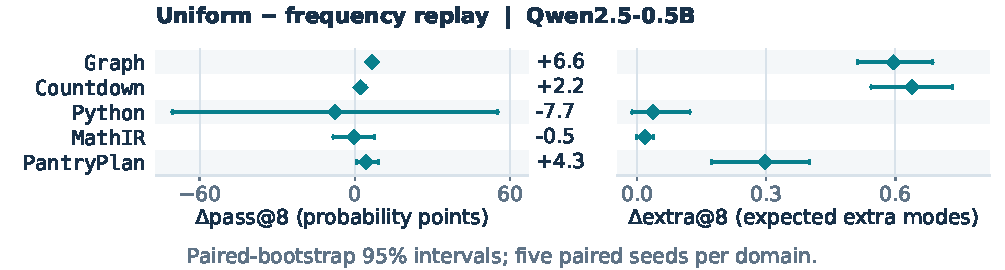
\includegraphics[width=\linewidth]{figures/replay_key_weighting.pdf}
\caption{\textbf{Uniform weighting preserves more verified alternatives.}
Uniform minus frequency-weighted replay at Qwen2.5-0.5B, Level 1, with five matched seeds. Extra modes are $B_8=\texttt{distinct@8}-\texttt{pass@8}$. Bars show nominal 95\% paired-seed bootstrap intervals. The mean gain is $.318$ extra modes, with an inconclusive correctness effect. Extra modes remain coupled to correctness; they do not measure success-conditional \pmd{}.}
\label{fig:replay-key-weighting}
\end{figure}

\clearpage
\section{Fixed Semantic-Entropy Factorials}
\label{app:semantic-current-factorial}
A fixed semantic-entropy bonus can be applied with or without verified replay.
Pantry semantic arms use the registered E85 repairs: original E81/E82/E83
Pantry runs received zero semantic advantage because of an outcome-key defect
and remain excluded. The historical Falcon factorial display had not applied
that repair; no value from its superseded Pantry column is reused here.
The matched four-arm studies compare its effect on Dr.GRPO, its effect on
Re:Dr.GRPO, and the difference of these effects. This restores the full
factorial detail beyond the main semantic-only comparator. We reconstruct
exact terminal four-draw endpoints under the current source-admission policy:
identical repeated metrics are deduplicated, unapproved conflicting retries
abort, and the previously excluded Falcon Countdown replay seed 59 remains
excluded. All three contrasts in that cell therefore use the common four
seeds 55--58; other 0.5B/1B cells use five. No old five-seed Falcon Countdown
interval is reused. Tables report paired seed means and pointwise Student-$t$
95\% intervals, without pooling models or domains.

The Qwen2.5-3B extension has only fixed seed 70 and no semantic-only arm.
Its on-replay comparison is descriptive, has no interval and cannot identify
a factorial interaction. These are fixed-coefficient experiments, not a
sweep over entropy strengths. Their endpoints do not establish that semantic
entropy reproduces the mechanism of a bank that revisits verified keys.
\begin{table}[H]
\centering
\caption{Qwen2.5-0.5B: fixed semantic-entropy effects. Without replay is semantic-only minus Dr.GRPO; on replay is semantic-plus-replay minus Re:Dr.GRPO; interaction subtracts the first effect from the second. Extra modes equal distinct@8 minus pass@8.}
\label{tab:semantic-current-qwen2505b}
\scriptsize
\setlength{\tabcolsep}{3pt}
\begin{tabular}{lr l rrr}
\toprule
Domain & $n$ & Contrast & $\Delta$ pass@8 & $\Delta$ distinct@8 & $\Delta$ extra modes \\
\midrule
Graph & 5 & Without replay & $0.002$ $[-0.028, 0.031]$ & $0.004$ $[-0.034, 0.041]$ & $0.002$ $[-0.010, 0.014]$ \\
Graph & 5 & On replay & $-0.002$ $[-0.027, 0.023]$ & $-0.022$ $[-0.179, 0.135]$ & $-0.020$ $[-0.161, 0.120]$ \\
Graph & 5 & Interaction & $-0.004$ $[-0.035, 0.028]$ & $-0.026$ $[-0.193, 0.141]$ & $-0.022$ $[-0.161, 0.116]$ \\
Countdown & 5 & Without replay & $0.141$ $[-0.047, 0.330]$ & $0.184$ $[0.011, 0.358]$ & $0.043$ $[0.001, 0.085]$ \\
Countdown & 5 & On replay & $-0.003$ $[-0.033, 0.028]$ & $0.115$ $[0.022, 0.209]$ & $0.118$ $[0.004, 0.232]$ \\
Countdown & 5 & Interaction & $-0.144$ $[-0.326, 0.037]$ & $-0.069$ $[-0.233, 0.095]$ & $0.075$ $[-0.051, 0.201]$ \\
Python & 5 & Without replay & $0.000$ $[0.000, 0.000]$ & $0.000$ $[0.000, 0.000]$ & $0.000$ $[0.000, 0.000]$ \\
Python & 5 & On replay & $-0.002$ $[-0.717, 0.714]$ & $0.016$ $[-0.747, 0.780]$ & $0.018$ $[-0.164, 0.200]$ \\
Python & 5 & Interaction & $-0.002$ $[-0.717, 0.714]$ & $0.016$ $[-0.747, 0.780]$ & $0.018$ $[-0.164, 0.200]$ \\
MathIR & 5 & Without replay & $-0.121$ $[-0.349, 0.106]$ & $-0.121$ $[-0.347, 0.105]$ & $0.001$ $[-0.006, 0.008]$ \\
MathIR & 5 & On replay & $0.031$ $[-0.035, 0.097]$ & $0.035$ $[-0.044, 0.114]$ & $0.004$ $[-0.047, 0.055]$ \\
MathIR & 5 & Interaction & $0.153$ $[-0.018, 0.324]$ & $0.156$ $[-0.050, 0.362]$ & $0.003$ $[-0.052, 0.058]$ \\
Pantry & 5 & Without replay & $0.201$ $[0.119, 0.283]$ & $1.120$ $[0.888, 1.352]$ & $0.919$ $[0.713, 1.124]$ \\
Pantry & 5 & On replay & $0.141$ $[0.044, 0.238]$ & $1.095$ $[0.368, 1.823]$ & $0.955$ $[0.321, 1.589]$ \\
Pantry & 5 & Interaction & $-0.061$ $[-0.161, 0.040]$ & $-0.025$ $[-0.826, 0.777]$ & $0.036$ $[-0.682, 0.754]$ \\
\bottomrule
\end{tabular}
\end{table}
\begin{table}[H]
\centering
\caption{Falcon3-1B: fixed semantic-entropy effects. Without replay is semantic-only minus Dr.GRPO; on replay is semantic-plus-replay minus Re:Dr.GRPO; interaction subtracts the first effect from the second. Extra modes equal distinct@8 minus pass@8.}
\label{tab:semantic-current-falcon31b}
\scriptsize
\setlength{\tabcolsep}{3pt}
\begin{tabular}{lr l rrr}
\toprule
Domain & $n$ & Contrast & $\Delta$ pass@8 & $\Delta$ distinct@8 & $\Delta$ extra modes \\
\midrule
Graph & 5 & Without replay & $0.036$ $[-0.192, 0.264]$ & $0.205$ $[-0.483, 0.893]$ & $0.169$ $[-0.292, 0.630]$ \\
Graph & 5 & On replay & $0.001$ $[-0.040, 0.043]$ & $-0.006$ $[-0.113, 0.101]$ & $-0.007$ $[-0.091, 0.077]$ \\
Graph & 5 & Interaction & $-0.035$ $[-0.237, 0.168]$ & $-0.211$ $[-0.886, 0.464]$ & $-0.176$ $[-0.649, 0.297]$ \\
Countdown & 4 & Without replay & $0.004$ $[-0.092, 0.100]$ & $-0.042$ $[-0.258, 0.173]$ & $-0.047$ $[-0.168, 0.074]$ \\
Countdown & 4 & On replay & $0.036$ $[-0.028, 0.101]$ & $0.047$ $[-0.082, 0.177]$ & $0.011$ $[-0.064, 0.087]$ \\
Countdown & 4 & Interaction & $0.032$ $[-0.098, 0.161]$ & $0.090$ $[-0.188, 0.367]$ & $0.058$ $[-0.099, 0.216]$ \\
Python & 5 & Without replay & $0.002$ $[-0.003, 0.008]$ & $0.002$ $[-0.003, 0.008]$ & $0.000$ $[0.000, 0.000]$ \\
Python & 5 & On replay & $-0.133$ $[-0.308, 0.043]$ & $-0.091$ $[-0.503, 0.321]$ & $0.042$ $[-0.296, 0.380]$ \\
Python & 5 & Interaction & $-0.135$ $[-0.310, 0.040]$ & $-0.093$ $[-0.507, 0.321]$ & $0.042$ $[-0.296, 0.380]$ \\
MathIR & 5 & Without replay & $-0.002$ $[-0.063, 0.060]$ & $-0.002$ $[-0.063, 0.060]$ & $0.000$ $[0.000, 0.000]$ \\
MathIR & 5 & On replay & $0.086$ $[0.004, 0.168]$ & $0.108$ $[0.003, 0.214]$ & $0.022$ $[-0.009, 0.054]$ \\
MathIR & 5 & Interaction & $0.087$ $[0.029, 0.146]$ & $0.110$ $[0.043, 0.176]$ & $0.022$ $[-0.009, 0.054]$ \\
Pantry & 5 & Without replay & $0.011$ $[-0.019, 0.041]$ & $0.091$ $[-0.161, 0.342]$ & $0.080$ $[-0.142, 0.301]$ \\
Pantry & 5 & On replay & $0.025$ $[-0.044, 0.094]$ & $0.382$ $[-0.702, 1.465]$ & $0.356$ $[-0.670, 1.382]$ \\
Pantry & 5 & Interaction & $0.014$ $[-0.052, 0.081]$ & $0.291$ $[-0.646, 1.228]$ & $0.277$ $[-0.615, 1.168]$ \\
\bottomrule
\end{tabular}
\end{table}
\begin{table}[H]
\centering
\caption{Qwen2.5-3B: fixed semantic-entropy effects. Without replay is semantic-only minus Dr.GRPO; on replay is semantic-plus-replay minus Re:Dr.GRPO; interaction subtracts the first effect from the second. Extra modes equal distinct@8 minus pass@8.}
\label{tab:semantic-current-qwen253b}
\scriptsize
\setlength{\tabcolsep}{3pt}
\begin{tabular}{lr l rrr}
\toprule
Domain & $n$ & Contrast & $\Delta$ pass@8 & $\Delta$ distinct@8 & $\Delta$ extra modes \\
\midrule
Graph & 1 & On replay & $-0.016$ & $-0.010$ & $0.006$ \\
Countdown & 1 & On replay & $0.039$ & $0.146$ & $0.107$ \\
Python & 1 & On replay & $-0.590$ & $-1.215$ & $-0.625$ \\
MathIR & 1 & On replay & $0.033$ & $0.010$ & $-0.023$ \\
Pantry & 1 & On replay & $0.035$ & $0.393$ & $0.357$ \\
\bottomrule
\end{tabular}
\end{table}
\path{results/semantic_current_summary_20260912.json} retains per-seed
endpoints, source hashes, exclusion evidence and all three metrics.
\path{ops/build_paper_semantic_current_summary.py} reconstructs these contrasts
with the same strict endpoint reader used by the current core comparison, including all documented exclusions.


\newpage
\section{Concentration and Replay Mechanisms}
\label{app:ablations}

\subsection{Concentration with 64 responses per prompt}
\label{app:fresh-concentration}

We evaluate initial and terminal checkpoints on the 128 held-out Level-1
\texttt{Graph} and \texttt{PantryPlan} prompts, drawing 64 responses per
prompt from new sampling streams. This evaluation is separate from the
32-response comparison in Fig.~\ref{fig:concentration-story}. It covers
Qwen2.5-0.5B, Falcon3-1B, and Qwen2.5-3B, with five training seeds for
Dr.GRPO, Re:Dr, MaxRL, and Re:Max. For each model, the five initial
evaluations use independent sampling from the same weights. Each initial
evaluation is paired with one training seed and shared across the four methods.

\paragraph{Matched comparisons.}
We estimate \pmd{} from correct-output pairs and average promptwise
differences over prompts with at least two correct responses in both
conditions, then average the five seed effects equally. Thus positive
changes indicate more diverse correct modes. Matching prompts within each
comparison differs from subtracting means over separately eligible prompts.
The eligible population ranges from 37 to 127 of the 128 prompts across
comparisons and seeds. Effects from different comparisons therefore cannot
be subtracted to reconstruct a trajectory on a common prompt population. Tables~\ref{tab:fresh-concentration-initial}
and~\ref{tab:fresh-concentration-replay} give all 36 contrasts and their
eligible-prompt ranges. Intervals are nominal 95\% paired Student-$t$
intervals with four degrees of freedom. They describe variation over the
five training-seed and initial-sampling pairs, conditional on the fixed
prompts and initial weights. They are unadjusted for multiple comparisons
and do not quantify uncertainty over unseen tasks.

\begin{figure}[t]
 \centering
 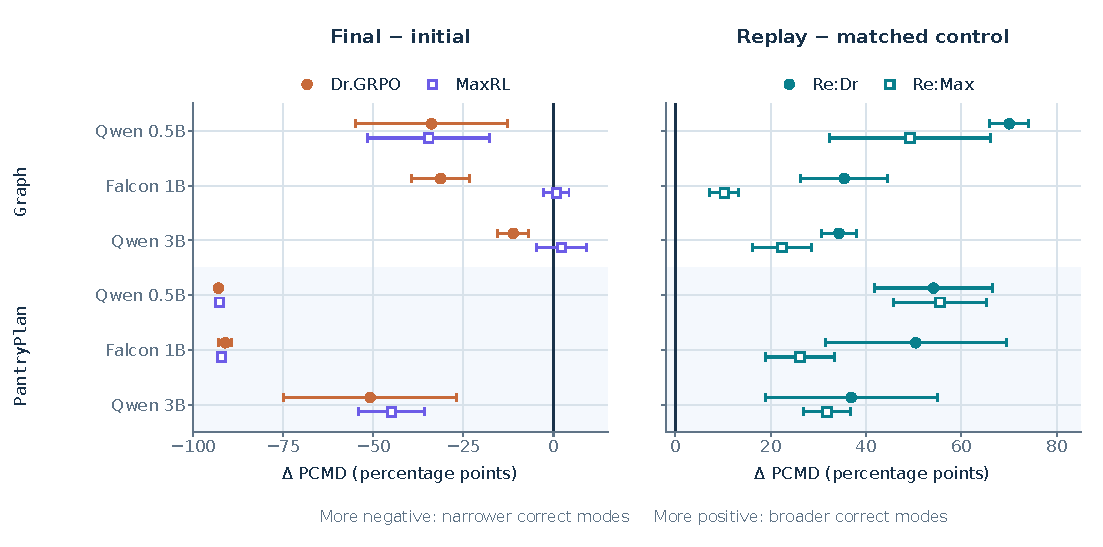
\includegraphics[width=\linewidth]{figures/fresh_concentration_pcmd_20260912.pdf}
 \caption{\textbf{Replay increases correct-mode diversity at a 64-response budget.}
 Left: Dr.GRPO reduces \pmd{} in all six model--domain comparisons;
 MaxRL's change is inconclusive for Falcon3-1B and Qwen2.5-3B \texttt{Graph}.
 Right: replay increases \pmd{} in all twelve comparisons with matched
 trained controls. Points show means over five paired seeds; bars give
 nominal 95\% Student-$t$ intervals. Each contrast uses its own jointly
 eligible Level-1 prompts. Horizontal scales differ between panels.}
 \label{fig:fresh-concentration}
\end{figure}

\paragraph{Concentration and mitigation.}
Dr.GRPO reduces \pmd{} in all six model--domain comparisons and all
30 seed effects. Replay increases \pmd{} relative to its matched trained
control under both objectives in all twelve comparisons and all 60 seed
effects. All eighteen nominal intervals exclude zero
(Fig.~\ref{fig:fresh-concentration}). These directions also hold when
pooling correct pairs, using each policy's own eligible prompts, or
restricting to the intersection of eligible prompts across seeds.
The intersection can be small: for Qwen2.5-0.5B \texttt{Graph}, only five
prompts are jointly eligible across all seeds in comparisons involving Dr.GRPO.

MaxRL alone does not consistently reduce diversity: its Falcon3-1B and
Qwen2.5-3B \texttt{Graph} intervals include zero. An improvement over a
trained control also need not restore initial diversity. Both replay
variants remain below initial \pmd{} in \texttt{PantryPlan} at every
scale, whereas their \texttt{Graph} comparisons exceed the initial value.
These results describe diversity within each comparison's eligible prompt
population; they do not establish recovery of the same individual modes.

\paragraph{Correctness, coverage, and sampling budget.}
All 24 trained-versus-initial comparisons increase per-response
correctness averaged over all evaluation prompts, in every seed. Nevertheless, every
\texttt{PantryPlan} method--scale comparison has lower \texttt{pass@64}
than initialization in every seed. Averaging over all evaluation prompts,
replay improves mean
\texttt{pass@8}, \texttt{distinct@8}, \texttt{pass@64}, and
\texttt{distinct@64} relative to its trained control in all twelve
comparisons; per-response correctness improves in seven of twelve.
On jointly eligible prompts, however, replay lowers mean correctness in
eleven of twelve comparisons. The concentration effects therefore do not
hold correctness fixed.

The eight-response metrics average over subsets of eight responses from
each 64-response pool (rarefaction). For Qwen2.5-3B \texttt{Graph}, Dr.GRPO increases per-response correctness by
14.49 percentage points and \texttt{distinct@8} by 0.112 modes per prompt,
while reducing \pmd{} by 11.20 points and \texttt{distinct@64} by
0.220 modes. The change in verified-mode count reverses sign between
eight and 64 responses in every seed. A gain at one sampling budget thus
need not persist at a larger budget. These evaluations measure the
distribution of correct responses and the modes observed in finite samples;
they do not establish exact mode extinction, recovery of the full support,
or a causal effect of diversity on accuracy.

\input{results/fresh_concentration_20260912_initial_table.tex}
\input{results/fresh_concentration_20260912_replay_table.tex}
\FloatBarrier


\subsection{Conditional concentration from saved training outputs}
\label{app:conditional-concentration}

This retrospective analysis distinguishes the distribution of correct keys
from the probability of producing a correct output. If $P=0$, $C$ is undefined
and $B_2=0$. For a fixed prompt with
correct mass $P>0$, write $q_c=\Pr[V(Y,s_x)=c\mid V(Y,s_x)\ne\bot]$ and define
\begin{equation}
 C(q)=\sum_c q_c^2,\qquad B_2=2P-P^2C(q).
 \label{eq:collision-breadth-bridge}
\end{equation}
The first quantity is the probability that two independent correct outputs
share a key. The second identity follows by expanding
$B_2=\sum_c[1-(1-Pq_c)^2]$. It makes explicit why sampled breadth can
change through correctness or conditional concentration. A decrease in $C$
alone does not imply majorization, larger total support, or recovery of any
particular mode. In particular, observed collisions cannot establish that
an unobserved key has exactly zero probability under the policy.

\paragraph{Connection to the conditional theory.}
Under the assumptions of Theorem~\ref{thm:grpo-collapse}, the time change in
its proof gives $dq_c/d\tau=q_c(q_c-C)$. Consequently,
\begin{equation}
 \frac{dC}{d\tau}
 =2\left(\sum_c q_c^3-C^2\right)
 =2\operatorname{Var}_{c\sim q}(q_c)\ge0.
 \label{eq:collision-flow}
\end{equation}
The variance vanishes exactly when $q$ is uniform on its positive support.
Thus concentration is monotone along this ideal categorical flow, with
strict increase whenever the positive coordinates are unequal. The identity
provides a theoretical basis for the diagnostic; it does not establish
monotonicity for the implemented neural optimizer or a corresponding
monotonic decrease under finite-bank replay.

\paragraph{Estimator and identifiable population.}
The pair statistic is the one defined in App.~\ref{app:metric-sampling}, read
here in the collision orientation, $\widehat C=1-\widehat{\pmd}$, over a prompt's
$R\ge2$ correct samples: the contrast this analysis reports is about
concentration, so the orientation that rises with it is the one to print. Its
promptwise unbiasedness, and the limits of that identity under joint selection,
are established there. We leave $R<2$ undefined, rather than assigning a
concentration value to insufficient correct observations.

For each paired training seed $s$, let $E_s$ contain exactly the prompts with
a defined estimate in both conditions. The reported seed contrast is
$|E_s|^{-1}\sum_{x\in E_s}(\widehat C_{B,x}-\widehat C_{A,x})$ when
$E_s$ is nonempty. We then weight defined training seeds equally, preserving
all registered blocks and their missingness. Before/after contrasts use each
method's own initial checkpoint and step 3,072; replay contrasts compare
matched terminal conditions. No other method substitutes for a missing
initial evaluation. Five defined seeds receive nominal Student-$t$ intervals;
partial blocks are descriptive. These intervals describe the measured seed
means and are not simultaneous guarantees or uncertainty over unseen prompts.

The hosted analysis uses the same promptwise collision concept but pools
correct pairs. At a common sampling budget, the ratio of expected colliding
and correct pair counts is
$\sum_x P_x^2 C(q_x)/\sum_x P_x^2$. Its finite-sample ratio is not generally
unbiased for that target. The training contrast here weights eligible prompts
equally. Changing correctness can change either eligibility or hosted pair
weights, so the two aggregate values are not directly interchangeable.

\paragraph{Retrospective protocol and source coverage.}
The estimator and comparisons were recorded before the initial concentration
contrasts, with the sampling-stream amendment also preceding those effects.
Two retrospective extensions then followed the paper's completed source
census. The first included thirteen newly available terminal checkpoints
and withdrew one conflicted initial checkpoint. The September~12 extension
adds all ten remaining Level-2 Pantry terminal checkpoints, reusing 752
unchanged checkpoint identities and changing no estimator or eligibility
rule. All prior results, caches, and source snapshots remain preserved.
The final collection contains 475 registered runs and 902 available
checkpoint evaluations, with 74 Dr.GRPO and 75 MaxRL Level-1 replay pairs
and 25 pairs per objective at Level~2 before conditional eligibility.
Complete terminal coverage neither supplies missing initial outputs nor
makes every conditional contrast identifiable. Exact source hashes and
both retrospective extensions' timing remain bound to the result artifact.

\paragraph{Sampling-stream audit.}
Four saved eight-output groups do not provide 32 independently seeded
responses. The recorded parent seeds increment by one; the audited vLLM V0
sampler increments each child's seed by its output index. The resulting
nominal stream ranges overlap, giving eleven distinct identifiers. For each
prompt and checkpoint we retain the earliest draw/output position for every
identifier, independently of correctness or key identity. Repeated positions
sometimes disagree, so identical seed integers are not treated as a proof of
identical outputs. Archived actor source is available for 150 of the 400
factorial cells and none of the 75 additional GRPO cells; historical dependency
identity is not cryptographically established for every run. The stream
mapping rests on the audited implementation and recorded neutral request
contract, with the historical-runtime assumption stated explicitly.

The primary eleven-stream comparisons reuse nominal streams across conditions
and remain descriptive after common eligibility. Two additional orientations
compare the lower five identifiers in condition A with the upper six in B,
then reverse the assignment. Each orientation retains its own eligible prompts
and seed counts. Shared identifiers also recur across prompts; neither their
separation across conditions nor these selected-population means establishes
independent prompt observations. Independent fixed-law sampling is an explicit
assumption of the estimator identity, not a conclusion of the source audit.

Original \texttt{mean@8}, \texttt{pass@8}, and \texttt{distinct@8} remain averages
over the four intact groups, reconstructed from all saved verified keys.
Cross-group overlap affects dependence, not linearity of those marginal
averages. The complete result artifact also retains each intact-group
collision comparison, a fixed-first-group check, fixed-across-seed prompt
intersections, and four-condition change differences. A naive concatenated
32-position collision is retained solely as a reuse diagnostic. These views
are not treated as independent replications or substituted for missing cells.

\paragraph{Findings and their limits.}
In Graph and PantryPlan, all twelve Dr.GRPO/GRPO before/after comparisons
across the three scales show increased conditional concentration, with
nominal intervals above zero. Correctness also increases on those same
eligible prompts. Graph's increases range from $.098$ to $.274$; PantryPlan's
range from $.447$ to $.887$. The two disjoint orientations agree in direction
in eleven of these twelve blocks; Falcon Graph with GRPO is the exception.
The evidence therefore supports observed training-induced concentration in
these tasks, with a visible sampling sensitivity, rather than a universal
claim about every RLVR run or exact disappearance of modes.

Re:Dr lowers concentration relative to Dr.GRPO in all six Graph and
PantryPlan comparisons: changes range from $-.756$ to $-.273$ in Graph and
$-.433$ to $-.300$ in PantryPlan. Both disjoint orientations agree in direction
in all six, and their primary nominal intervals lie below zero. These
comparisons also have lower per-sample correctness on their jointly eligible
prompts. They establish a change in the conditional correct-key distribution
on that observable population; they do not hold correctness fixed or imply
that every accuracy measure improves on the same prompts. Full-test
\texttt{pass@8} and sampled breadth remain the separately reported primary
outcomes of the replay experiment.

The other domains constrain the interpretation. Dr.GRPO/GRPO Python initial
outputs provide no jointly eligible prompts at this budget, so their
longitudinal collision contrast is unidentified. Some Countdown initial
comparisons use only one or two eligible prompts per seed. Several MathIR
conditions already have observed collision one, leaving little detectable
change. MaxRL comparisons, incomplete saved-output cohorts, and the two
sampling orientations are reported explicitly in the following tables;
we do not infer a universal concentration benefit from raw breadth gains.

In the completed 3B MaxRL replay cohort, Countdown, Python, and PantryPlan
show lower concentration with nominal intervals below zero; MathIR's measured
contrast is zero. Graph's primary contrast is negative, but its two disjoint
orientations disagree in direction, as they do for Falcon Graph with MaxRL.
At Level 2, both Graph replay contrasts are negative with agreement across
orientations. Complete PantryPlan training still leaves sparse conditional
populations: Re:Dr has a defined collision contrast for three seeds
(2--16 eligible prompts), with mean $+.495$; Re:Max has four defined
seeds (1--19 eligible prompts), with mean $+.439$. Their disjoint-orientation
means are also positive but retain fewer defined seeds. Neither contrast
receives a five-seed interval. Thus the full endpoint breadth gains coexist
with increased concentration on these small jointly correct subsets; they
do not establish uniformly reduced conditional concentration.

\input{results/conditional_concentration_20260912_tables.tex}


\begin{figure}[!htbp]
  \centering
  % One float, two panels: the same contrast read along the scale axis and
  % along the level axis. Equal minipage widths and matched native plate
  % widths, so neither panel is magnified relative to the other.
  \begin{minipage}[t]{.49\linewidth}
    \centering
    \textbf{(A)}\\[1pt]
    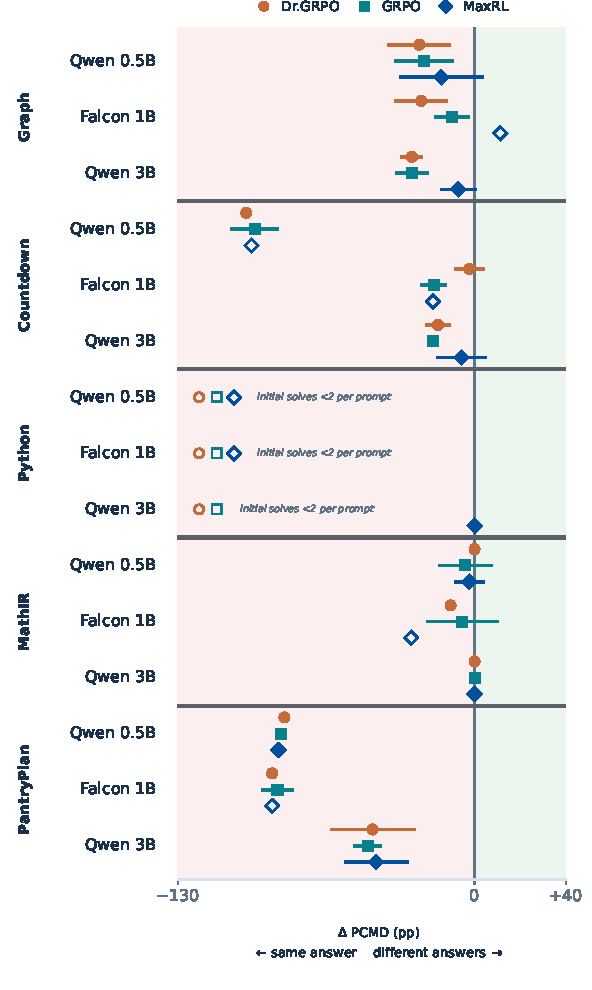
\includegraphics[width=\linewidth]{figures/concentration_story_all_scales.pdf}
  \end{minipage}\hfill
  \begin{minipage}[t]{.49\linewidth}
    \centering
    \textbf{(B)}\\[1pt]
    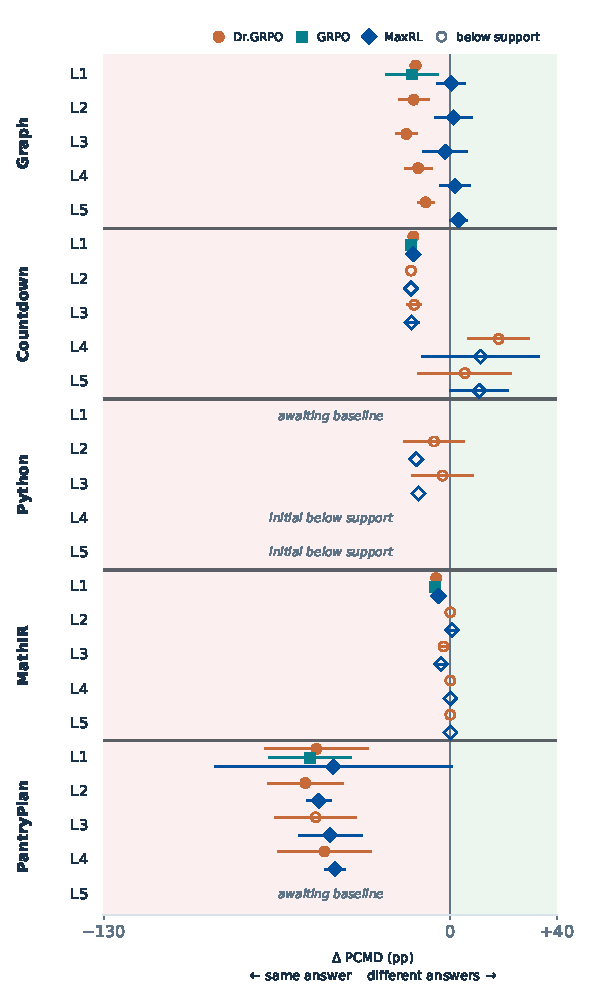
\includegraphics[width=\linewidth]{figures/concentration_levels.pdf}
  \end{minipage}
  \caption{\textbf{\texttt{Graph} and \texttt{PantryPlan} lose conditional solution diversity
  across scales and task levels.} Changes in \pmd{}, in percentage points.
  \textbf{(A)} Initial-to-final changes at Level~1 across three model scales
  and three objectives. Each seed averages over prompts with at least two
  correct responses at both checkpoints. Filled marks and bars show five-seed
  means and nominal paired 95\% Student-$t$ intervals. Open marks show
  means from fewer than five seeds, without intervals; annotated hollow
  symbols identify methods with no jointly eligible prompts. Dr.GRPO and GRPO reduce
  diversity in \texttt{Graph} and \texttt{PantryPlan} at every scale.
  \textbf{(B)} Level-1-trained policies evaluated on Levels~1--5, with
  Levels~2--5 measuring transfer. Available evaluations are averaged within
  each scale, then scales receive equal weight. Evaluations with different
  context limits contribute separately within a scale but do not constitute
  additional training seeds. Each scale uses one initial checkpoint evaluation.
  Bars appear only when one scale contributes and give nominal 95\%
  Student-$t$ intervals over its training seeds. Open marks indicate that at
  least one contributing scale has fewer than 30 eligible initial prompts or
  fewer than 30 eligible trained prompt observations in total. Missing initial
  references have fewer than two eligible prompts. GRPO appears only at
  Level~1. \texttt{Graph} and \texttt{PantryPlan} means decrease at every level; \texttt{Countdown}
  increases at Levels~4--5.}
  \label{fig:concentration-all-scales}
  \label{fig:concentration-levels}
\end{figure}


\subsection{Diversity before and after RLVR-only training}
\label{app:pre-rl-regression}

We evaluate Dr.GRPO and GRPO before training and after eight passes across
three models and five domains. The 150 runs each use four $K=8$ response
groups per checkpoint. Averaged equally across the five domains, extra
verified modes decrease by $98.2\%$--$99.4\%$ at Qwen2.5-0.5B and
$41.5\%$--$71.6\%$ at larger scales. The \texttt{pass@8} mean falls in
10 of the 30 domain--method--scale comparisons, while macro
\texttt{distinct@8} ends above its initial value at Qwen2.5-3B.
Fewer extra verified modes can therefore coexist with a greater probability
of sampling at least one correct response. Finite samples do not establish
that unobserved solution keys have zero probability.

\begin{samepage}
The domain average of \pmd{} includes only domains measurable at both endpoints: \texttt{Graph}, \texttt{MathIR}, and
\texttt{PantryPlan} at 0.5B; \texttt{Graph}, \texttt{Countdown}, and \texttt{PantryPlan} at 1B; and \texttt{Graph} and
\texttt{PantryPlan} at 3B. It declines by $98.5\%$ and $99.7\%$ at Qwen2.5-0.5B under
GRPO and Dr.GRPO, respectively, and by $50.8\%$--$65.1\%$ at the larger
scales. Terminal macro \pmd{} rounds to $.001$ for Dr.GRPO at Qwen2.5-0.5B.
The decline thus also appears in diversity conditional on success. Because
eligibility depends on the number of correct samples, these descriptive
averages do not hold the prompt population or correctness fixed.
App.~\ref{app:conditional-concentration} reports contrasts on jointly eligible
prompts. The decline is not universal: Falcon3-1B \texttt{Countdown} has
increasing \pmd{} under Dr.GRPO, from an initial value of $.033$.

\end{samepage}

Although the initial weights are shared, each method uses its own evaluation
samples. Differences between initial estimates therefore reflect sampling
variability.

\begin{figure}[t]
  \centering
  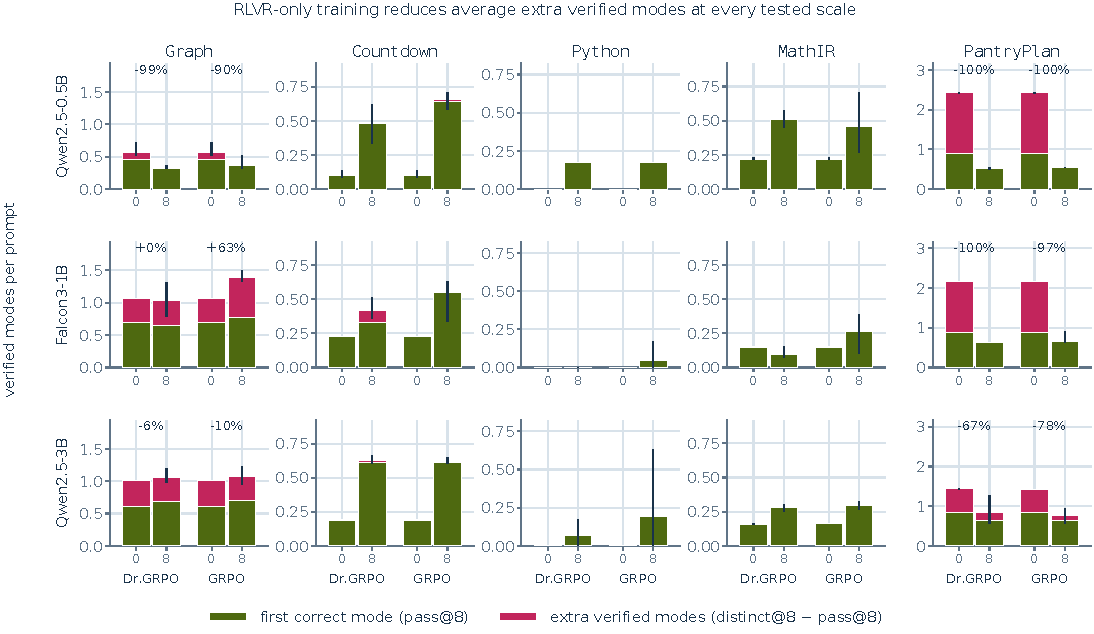
\includegraphics[width=\linewidth]{figures/baseline_collapse_precheck.pdf}
  \caption{\textbf{RLVR-only training reduces average extra verified modes
  at every tested scale.} Bars decompose \texttt{distinct@8} into
  \texttt{pass@8} and extra verified modes before training and after eight
  passes. Panels show Dr.GRPO and GRPO across three models and five domains:
  150 runs, with five seeds per model--domain--method combination and four
  eight-response groups per checkpoint. Whiskers show seed ranges; each
  method uses its own initial evaluation. Percentage changes in extra modes
  are shown for \texttt{Graph} and \texttt{PantryPlan}, whose initial means
  exceed $.05$. The other three domains start at $.011$ or less.}
  \label{fig:baseline-precheck}
\end{figure}




\texttt{Graph} and \texttt{PantryPlan} have substantial initial diversity at every
scale, whereas the other domains start with at most $.011$ extra modes per
prompt. To avoid unstable ratios near zero, retained-diversity percentages
are reported only when the initial extra-mode count exceeds $.05$.
The final $\texttt{distinct@8}$ is below its initial value in six of the
15 Dr.GRPO model--domain combinations. For Re:Dr, this occurs in two
available comparisons, both on \texttt{PantryPlan}; Falcon3-1B
\texttt{Countdown} uses four seeds. Conditional diversity comparisons
also depend on which prompts yield enough correct responses.
App.~\ref{app:conditional-concentration} reports paired contrasts on
jointly eligible prompts, including seed counts and uncertainty. These
held-out evaluations do not track individual modes stored during training.

Uniform sampling over the enumerable action representations gives a
diversity reference for \texttt{Graph} and \texttt{PantryPlan}
(App.~\ref{app:metric-sampling}). No corresponding reference is specified
for the other domains. On \texttt{PantryPlan}, uniform sampling of bit
masks yields higher expected \texttt{distinct@8} than the final sampled
value of every model under both Dr.GRPO and Re:Dr.

\begin{table}[t]
  \centering
  \caption{\textbf{Uniform actions and untrained checkpoints provide absolute diversity references.}
  \emph{Uniform} gives expected \distk{} under uniform sampling of the
  action representation: 27 color strings for \texttt{Graph} and 64 bit masks
  for \texttt{PantryPlan}. \emph{Initial} gives the Dr.GRPO pass-0 reference;
  the final two columns give sampled means after eight training passes.}
  \label{tab:absolute-support-references}
  \scriptsize
  \setlength{\tabcolsep}{4.2pt}
  \begin{tabular}{@{}llrrrr@{}}
    \toprule
    \textbf{Model} & \textbf{Domain} & \textbf{Uniform} & \textbf{Initial}
      & \textbf{Dr.GRPO} & \textbf{Re:Dr} \\
    \midrule
        \qwenmark{}2.5-0.5B & \texttt{Graph} & 1.633 & .561 & .325 & 2.438 \\
     & \texttt{PantryPlan} & 2.153 & 2.426 & .522 & 1.539 \\
    \addlinespace[2pt]
    Falcon3-1B & \texttt{Graph} & 1.633 & 1.070 & 1.034 & 1.717 \\
     & \texttt{PantryPlan} & 2.153 & 2.162 & .633 & 1.576 \\
    \addlinespace[2pt]
    \qwenmark{}2.5-3B & \texttt{Graph} & 1.633 & 1.012 & 1.060 & 1.637 \\
     & \texttt{PantryPlan} & 2.153 & 1.445 & .841 & 1.514 \\
    \bottomrule

  \end{tabular}
\end{table}


\subsection{Vanishing task gradients and repeated outputs}
\label{app:degenerate-groups}

A Dr.GRPO group with identical rewards has exactly zero fresh task gradient.
Only mixed groups, containing both correct and incorrect responses,
provide a nonzero task advantage. Optimizer momentum can still change the
policy when the current task gradient is zero. The table below reports
the fraction of mixed groups over 3,072 Qwen2.5-0.5B updates, averaged
across five seeds.

\begin{center}
\small
\begin{tabular}{@{}lrr@{}}
\toprule
\textbf{Domain} & \textbf{Dr.GRPO} & \textbf{Re:Dr} \\
\midrule
\texttt{Graph} & .144 & .954 \\
\texttt{Countdown} & .140 & .456 \\
\texttt{Python} & .015 & .185 \\
\texttt{MathIR} & .364 & .453 \\
\texttt{PantryPlan} & .123 & .789 \\
\bottomrule
\end{tabular}
\end{center}

Thus 98.5\% of \texttt{Python} control updates carry zero fresh task gradient.
Replay contributes a likelihood gradient from verified responses and can
also change the policy so that subsequent fresh groups contain both correct
and incorrect responses.

All five Qwen2.5-0.5B \texttt{Python} control seeds exhibit observed output collapse.
At pass 0, eight-response groups average 7.99 distinct completion strings
per prompt. By steps 288--480, all 32 temperature-1 responses for each
prompt are identical within each seed and match its greedy completion.
This holds on all 128 prompts and persists at every subsequent evaluation
through step 3,072. The 32 responses span four groups with overlapping sampling
streams (App.~\ref{app:conditional-concentration}); they are not 32 independent
draws. Within eight-response groups, the terminal mean is 1.00 distinct
completion per prompt for the control and 1.97 for replay. The repeated
completion can be incorrect. These finite observations do not rule out
low-probability alternatives.

This sparse binary-reward setting allows fresh task gradients to vanish.
Sampling strategies that favor mixed groups, larger groups, a reference-policy
KL penalty, token-entropy regularization, or broader decoding could change
this behavior. The present comparison does not isolate their effects.

\subsection{The controls learn at the fixed learning rates}
\label{app:control-learning-audit}

The controls use a constant learning rate of $2\times10^{-7}$ at
Qwen2.5-0.5B and Falcon3-1B and a peak rate of $10^{-7}$ with cosine decay
at Qwen2.5-3B (Table~\ref{tab:run-contract}). Learning rates are not swept.
Table~\ref{tab:control-learning-audit} reports changes in accuracy and the
frequency of informative response groups under these schedules. The
results characterize the tested settings without identifying an optimal
schedule for either method.

\begin{table}[t]
  \centering
  \caption{\textbf{Per-response accuracy increases in every control comparison,
  while \texttt{pass@8} can fall.} Accuracy compares initial and last
  available evaluations. Columns show unpaired five-run means for each
  model--domain combination. \texttt{mean@8} measures per-response
  correctness. Mixed gives the mean fraction of rollout groups
  containing both correct and incorrect responses. An unmixed group has
  zero fresh task advantage, although optimizer momentum can still change
  the policy. Training schedules match update counts and fresh-rollout
  budgets; total compute is discussed in App.~\ref{app:compute-accounting}.}
  \label{tab:control-learning-audit}
  \small
  \setlength{\tabcolsep}{5pt}
  \begin{tabular}{@{}llrrrrrrr@{}}
    \toprule
    & & \multicolumn{3}{c}{\textbf{control \texttt{pass@8}}}
      & \multicolumn{2}{c}{\textbf{control \texttt{mean@8}}}
      & \textbf{mixed} & \textbf{Re:Dr} \\
    \cmidrule(lr){3-5}\cmidrule(lr){6-7}
    \textbf{Model} & \textbf{Domain} & initial & terminal & $\Delta$
      & initial & terminal & groups & \texttt{pass@8} \\
    \midrule
    % Generated by ops/build_paper_control_learning_audit.py; do not hand edit.
    Qwen2.5-0.5B & \texttt{Graph} & .456 & .323 & $-$.132 & .178 & .323 & .144 & .969 \\
     & \texttt{Countdown} & .097 & .480 & $+$.383 & .014 & .465 & .140 & .672 \\
     & \texttt{Python} & .000 & .172 & $+$.172 & .000 & .172 & .015 & .528 \\
     & \texttt{MathIR} & .220 & .512 & $+$.292 & .037 & .464 & .364 & .796 \\
     & \texttt{PantryPlan} & .902 & .522 & $-$.380 & .344 & .522 & .123 & .729 \\
    \addlinespace[2pt]
    Falcon3-1B & \texttt{Graph} & .693 & .656 & $-$.037 & .178 & .300 & .777 & .809 \\
     & \texttt{Countdown} & .225 & .328 & $+$.103 & .037 & .268 & .400 & .636 \\
     & \texttt{Python} & .000 & .000 & $+$.000 & .000 & .000 & .009 & .979 \\
     & \texttt{MathIR} & .148 & .095 & $-$.053 & .023 & .068 & .158 & .736 \\
     & \texttt{PantryPlan} & .891 & .633 & $-$.258 & .318 & .633 & .523 & .751 \\
    \addlinespace[2pt]
    Qwen2.5-3B & \texttt{Graph} & .607 & .682 & $+$.075 & .215 & .360 & .706 & .836 \\
     & \texttt{Countdown} & .184 & .609 & $+$.426 & .049 & .569 & .281 & .746 \\
     & \texttt{Python} & .000 & .069 & $+$.069 & .000 & .069 & .011 & .659 \\
     & \texttt{MathIR} & .156 & .278 & $+$.122 & .061 & .168 & .152 & .686 \\
     & \texttt{PantryPlan} & .831 & .638 & $-$.193 & .267 & .558 & .482 & .744 \\
    \bottomrule

  \end{tabular}
\end{table}

\paragraph{Accuracy changes during training.}
Per-response correctness (\texttt{mean@8}) rises in all 15
control comparisons: every control learns under its schedule. What varies
is coverage. Using an absolute-change threshold of $.005$, 8 of the
15 comparisons improve in \texttt{pass@8} and
6 decline, so 7 controls gain per-response accuracy
without a \texttt{pass@8} increase above that threshold. The mean
\texttt{pass@8} change is +0.039; the largest increase is $+0.426$
(\texttt{Countdown} at Qwen2.5-3B) and the largest decrease is $-0.380$
(\texttt{PantryPlan} at Qwen2.5-0.5B). In \texttt{PantryPlan} at Falcon3-1B, per-response correctness rises from
0.318 to 0.633, while \texttt{pass@8}
falls from 0.891 to 0.633.
This combination is consistent with prior observations of increased
single-response accuracy alongside reduced sampling coverage
\citep{yue2025rlvrlimit}.

The gap between \texttt{pass@8} and \texttt{mean@8} is at least $.02$ in
12 initial model--domain comparisons and below $.02$ in
7 terminal comparisons. This gap reflects variation in
correctness within response groups; it does not identify repeated strings
or conditional diversity among correct solution keys. The completion-string
analysis in App.~\ref{app:degenerate-groups} directly measures repetition
for the Qwen2.5-0.5B \texttt{Python} controls.

\paragraph{Sparse fresh reward information.}
Initial \texttt{pass@8} is zero on \texttt{Python} at all three
scales. In \texttt{Python} at Falcon3-1B, only a fraction 0.009 of
updates contain mixed rewards, leaving zero fresh task advantage in
99.1\% of updates. A learning-rate change cannot make an
identically zero current task gradient nonzero, but it can change the effect
of informative updates, optimizer momentum, and subsequent sampling.
The Falcon3-1B \texttt{Python} control's terminal \texttt{pass@8} rounds to $.000$, while Re:Dr
ends at $.979$. This is an accuracy contrast in a sparse-success setting;
conditional mode diversity requires at least two correct responses per
prompt and is undefined when that sampling condition is unmet.

\paragraph{Scope of the comparison.}
Replay and control share the learning rate, schedule, initialization,
prompt stream, optimizer, update count, and fresh-rollout budget.
The comparison measures the effect of replay under these settings.
Per-response correctness increases in the controls, but the absence of a
learning-rate sweep limits conclusions about their optimal performance.
Other learning rates could change accuracy, diversity, and the relative
benefit of replay; the present results do not determine those changes.

The frequency of mixed groups helps characterize these comparisons.
When a control rarely produces mixed groups (App.~\ref{app:degenerate-groups}),
replay provides a likelihood gradient on updates with no fresh task advantage.
We therefore also summarize replay effects in subsets with increasing
control accuracy. Across all 15 model--domain combinations, the mean
Re:Dr minus Dr.GRPO effect is $+.352$ in \texttt{pass@8} and $+.189$
in \pmd{}. Among the 9 combinations with any positive initial-to-final
change in control \texttt{pass@8}, the effects are $+.379$ and $+.118$.
Among the 6 that also have nonzero initial \texttt{pass@8} and at least
10\% mixed rollout groups, they are $+.247$ and $+.136$. Every comparison
in these subsets has positive effects on both metrics; the smallest effects
in the six-comparison subset are $+.137$ in \texttt{pass@8} and $+.013$
in \pmd{}. Its mean diversity effect is about two thirds of the mean
across all comparisons. Table~\ref{tab:control-learning-audit} gives the
control measurements that define these subsets.

\subsection{Likelihood changes with a fixed replay buffer}
\label{app:fixed-bank-survival}

We examine the likelihoods of stored responses during Qwen2.5-0.5B Re:Dr
training on \texttt{Graph}, using five seeds. The buffer contents and counts
of fresh verified responses are held fixed from immediately before the
fresh rollout at step 384. Uniform replay continues through step 3,072
without adding modes. For each stored exemplar, identified by prompt and
canonical mode, we measure mean token log probability $s$ and sequence
log probability $\ell$ whenever it is replayed. Changes compare its first
and final replay visits after the buffer is fixed; these steps can differ
across exemplars.

The 3,406 exemplars span 1,575 seed--prompt pairs, with 8--9 replay visits
per exemplar.
The pooled median change is $+.038$ nat/token (95\% interval
$[+.025,+.048]$), while the 10th percentile is $-.256$ and $2.61\%$ of
exemplars lose more than $.5$ nat/token ($[1.54,3.77]\%$).
The largest observed intermediate decrease is $-1.328$ nat/token. Sequence log
probability has median change $+.154$ nat/sequence ($[+.104,+.198]$),
with $21.99\%$ of exemplars losing more than $.5$ nat/sequence.
Lengths range from 4 to 100 tokens, so the token and sequence thresholds
measure different changes.

\begin{figure}[!htbp]
  \centering
  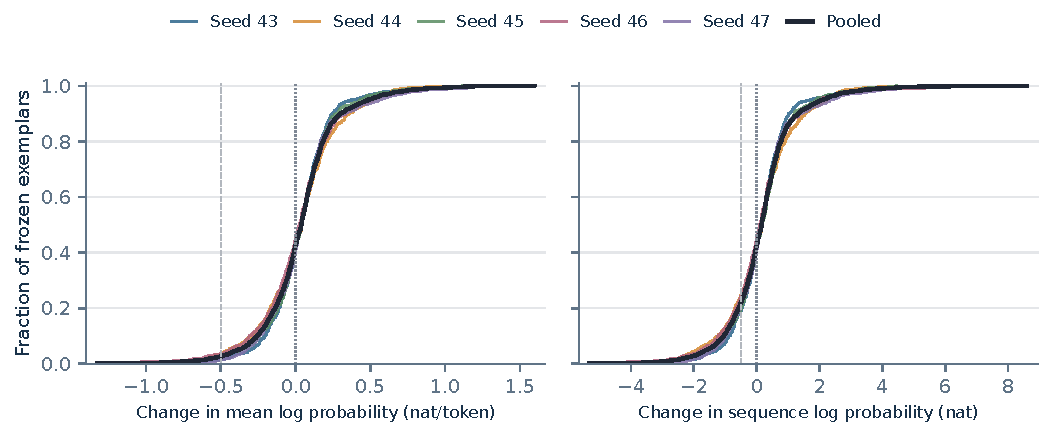
\includegraphics[width=.95\linewidth]{figures/e121_fixed_bank_survival.pdf}
  \caption{\textbf{Median exemplar scores rise, while some exemplars decline.}
  Empirical cumulative distributions of first-to-final score changes for
  3,406 fixed-buffer exemplars from five Qwen2.5-0.5B Re:Dr \texttt{Graph} seeds.
  Panels show mean token and sequence log probability. Colored curves
  represent individual seeds; the pooled curve weights exemplars equally.
  Dotted and dashed vertical lines mark zero and $-.5$, respectively.
  Positive changes indicate higher likelihood for the stored token sequence.
  Sequence likelihood does not measure the total probability of generating
  a canonical solution mode.}
  \label{fig:e121-fixed-bank-survival}
\end{figure}

Pooled summaries weight exemplars equally. Descriptive 95\% percentile
intervals use 10,000 hierarchical bootstrap replicates, resampling prompts
with replacement within each training seed and then resampling the five
seeds with replacement.

Scores are measured at replay visits, so changes between visits are
unobserved. Some stored exemplars lose likelihood despite continued replay.
A matched fixed-buffer control without replay would be needed to isolate
the effect of replay. These sequence-level observations also do not test
the mode-probability floor in Theorem~\ref{thm:replay-retention}.

\clearpage
\phantomsection
\begin{center}\large\textbf{Part IV. What diversity represents}\end{center}
\addcontentsline{toc}{part}{Part IV. What diversity represents}

\section{Matched Prompt-Hint Ablation}
\label{app:prompt-hint-ablation}

\subsection{Removing strategy hints from unchanged problems}

\label{sec:prompt-hint-ablation}

We compare original and neutral prompts on \texttt{Python}, \texttt{MathIR}, and \texttt{PantryPlan} at Levels 2 and 3. Each of the six domain--level combinations uses 32 problems selected independently of model outputs from the 128-problem evaluation split. We sample eight responses per problem under each wording. The original wording uses the standard prompt. The neutral wording removes the \texttt{Python} nested-conditional example and suggestions to test small divisors or dispatch on listed values, the \texttt{MathIR} ordered algebraic-isolation suggestion, and the \texttt{PantryPlan} preference for ingredients high in energy and protein but low in sodium such as seeds or oats. \texttt{MathIR} changes ``those operations'' to ``the operations'' to preserve the instruction to return a menu ID. The problem instance, answer specification, executable verifier, and remaining format requirements are unchanged.

The paired effects are neutral minus original on empirical $P_8=\texttt{pass@8}$ and $D_8=\texttt{distinct@8}$, with $B_8=D_8-P_8$ as extra verified modes per problem. Incorrect, empty, and truncated outputs remain in their eight-draw groups; only verifier-accepted outputs contribute a verified key. Results use strict verification. A sensitivity analysis with normalized formatting preserves every strict success and canonical key and applies the same rules to both arms.

Intervals use 20,000 whole-problem bootstrap resamples, paired across arms and stratified by domain and level. Domain--level combinations receive equal weight in aggregate estimates. The intervals are pointwise 95\% percentile intervals without multiplicity adjustment. With 32 problems per domain and level, an interval crossing zero does not establish equivalence. A zero-width interval reflects zero variation in the observed bootstrap resamples, including identical paired $P_8$ outcomes, and does not establish population equivalence. Correct-pair collision and its certified-support uniform reference use the same correct-pair weights. Eight draws per prompt do not identify total unseen support.



We evaluate the initial Qwen2.5-0.5B-Instruct checkpoint and Level-2-trained Dr.GRPO and Re:Dr checkpoints. \texttt{Python} and \texttt{MathIR} use five matched training seeds; \texttt{PantryPlan} uses two. Level 3 tests transfer from Level 2 training. All checkpoints evaluate the same selected problems under the benchmark syntax constraints and a 192-token generation budget. Five-seed intervals resample whole training seeds and paired problems; \texttt{PantryPlan} intervals condition on its two checkpoints, and initial-model intervals condition on one instruction-tuned checkpoint. These effects concern the specified models, problems, and interface.


\begin{table}[t]
\centering
\scriptsize
\setlength{\tabcolsep}{2.2pt}
\caption{\textbf{Removing \texttt{Python} guidance reduces correctness and observed breadth.} Qwen2.5-0.5B checkpoints under strict verification, with original $\to$ neutral wording. $P_8=\texttt{pass@8}$, $D_8=\texttt{distinct@8}$, and $B_8=D_8-P_8$ use eight draws on each of 32 problems per domain and level. Effects are neutral minus original. $P_8$, $D_8$, and $B_8$ average the displayed number $s$ of checkpoints. Brackets are pointwise 95\% bootstrap intervals: paired problems and training seeds are resampled for five-seed groups; \texttt{PantryPlan} intervals condition on its two checkpoints, and initial-model intervals on one checkpoint. \pmd{} estimates the probability that two correct responses have different canonical keys, averaging checkpoint--problem groups with at least two verified draws in each arm. Its paired population depends on correctness, and repeated problems at different checkpoints count separately. Only 5 of 18 comparisons meet the minimum of 30 such groups; dashes denote the others. These \pmd{} point estimates have no reported uncertainty intervals.}
\label{tab:prompt-hints-local-strict}
\resizebox{\linewidth}{!}{%
\begin{tabular}{llrrrrrrr}
\toprule
Model & Domain/level & $P_8$: O$\to$N & $D_8$: O$\to$N & $\Delta P_8$ [95\%] & $\Delta D_8$ [95\%] & $\Delta B_8$ & \pmd{}: O$\to$N & $\Delta$ \pmd{} \\
\midrule
Initial ($s=1$) & \texttt{Python} L2 & $0.656\to0.125$ & $0.69\to0.12$ & $-0.531\;[-0.719,-0.344]$ & $-0.56\;[-0.75,-0.38]$ & $-0.03$ & -- & -- \\
Initial ($s=1$) & \texttt{MathIR} L2 & $0.250\to0.281$ & $0.25\to0.28$ & $+0.031\;[+0.000,+0.094]$ & $+0.03\;[+0.00,+0.09]$ & $+0.00$ & -- & -- \\
Initial ($s=1$) & \texttt{PantryPlan} L2 & $0.156\to0.188$ & $0.19\to0.22$ & $+0.031\;[+0.000,+0.094]$ & $+0.03\;[+0.00,+0.09]$ & $+0.00$ & -- & -- \\
Initial ($s=1$) & \texttt{Python} L3 & $0.719\to0.031$ & $0.81\to0.03$ & $-0.688\;[-0.844,-0.531]$ & $-0.78\;[-0.97,-0.59]$ & $-0.09$ & -- & -- \\
Initial ($s=1$) & \texttt{MathIR} L3 & $0.219\to0.219$ & $0.22\to0.22$ & $+0.000\;[-0.125,+0.125]$ & $+0.00\;[-0.12,+0.12]$ & $+0.00$ & -- & -- \\
Initial ($s=1$) & \texttt{PantryPlan} L3 & $0.281\to0.312$ & $0.66\to0.69$ & $+0.031\;[+0.000,+0.094]$ & $+0.03\;[-0.06,+0.12]$ & $+0.00$ & -- & -- \\
Dr.GRPO ($s=5$) & \texttt{MathIR} L2 & $0.531\to0.506$ & $0.53\to0.51$ & $-0.025\;[-0.100,+0.031]$ & $-0.03\;[-0.10,+0.03]$ & $+0.00$ & $.000\to.000$ & $+.000$ \\
Dr.GRPO ($s=5$) & \texttt{MathIR} L3 & $0.194\to0.156$ & $0.19\to0.16$ & $-0.037\;[-0.113,+0.019]$ & $-0.04\;[-0.11,+0.02]$ & $+0.00$ & -- & -- \\
Dr.GRPO ($s=2$) & \texttt{PantryPlan} L2 & $0.219\to0.203$ & $0.28\to0.25$ & $-0.016\;[-0.156,+0.125]$ & $-0.03\;[-0.19,+0.12]$ & $-0.02$ & -- & -- \\
Dr.GRPO ($s=2$) & \texttt{PantryPlan} L3 & $0.172\to0.172$ & $0.27\to0.25$ & $+0.000\;[-0.078,+0.078]$ & $-0.02\;[-0.16,+0.11]$ & $-0.02$ & -- & -- \\
Dr.GRPO ($s=5$) & \texttt{Python} L2 & $0.812\to0.000$ & $0.81\to0.00$ & $-0.812\;[-0.938,-0.656]$ & $-0.81\;[-0.94,-0.66]$ & $+0.00$ & -- & -- \\
Dr.GRPO ($s=5$) & \texttt{Python} L3 & $1.000\to0.000$ & $1.00\to0.00$ & $-1.000\;[-1.000,-1.000]$ & $-1.00\;[-1.00,-1.00]$ & $+0.00$ & -- & -- \\
Re:Dr ($s=5$) & \texttt{MathIR} L2 & $0.994\to0.975$ & $0.99\to0.97$ & $-0.019\;[-0.075,+0.000]$ & $-0.02\;[-0.07,+0.00]$ & $+0.00$ & $.000\to.000$ & $+.000$ \\
Re:Dr ($s=5$) & \texttt{MathIR} L3 & $0.312\to0.275$ & $0.31\to0.28$ & $-0.037\;[-0.138,+0.044]$ & $-0.04\;[-0.14,+0.04]$ & $+0.00$ & $.000\to.000$ & $+.000$ \\
Re:Dr ($s=2$) & \texttt{PantryPlan} L2 & $0.516\to0.500$ & $0.75\to0.73$ & $-0.016\;[-0.109,+0.078]$ & $-0.02\;[-0.20,+0.17]$ & $+0.00$ & -- & -- \\
Re:Dr ($s=2$) & \texttt{PantryPlan} L3 & $0.234\to0.281$ & $0.39\to0.50$ & $+0.047\;[+0.000,+0.109]$ & $+0.11\;[+0.05,+0.19]$ & $+0.06$ & -- & -- \\
Re:Dr ($s=5$) & \texttt{Python} L2 & $0.887\to0.556$ & $1.24\to0.68$ & $-0.331\;[-0.525,-0.150]$ & $-0.57\;[-0.85,-0.32]$ & $-0.24$ & $.231\to.173$ & $-.058$ \\
Re:Dr ($s=5$) & \texttt{Python} L3 & $1.000\to0.494$ & $1.42\to0.66$ & $-0.506\;[-0.825,-0.194]$ & $-0.76\;[-1.07,-0.38]$ & $-0.26$ & $.256\to.323$ & $+.067$ \\
\bottomrule
\end{tabular}}
\end{table}


\pmd{} is reported for five of the 18 comparisons in Table~\ref{tab:prompt-hints-local-strict}. Each requires at least thirty checkpoint--problem groups with at least two verified draws under each wording. The same 32 problems are evaluated at each checkpoint, so these group counts include repeated problems across training seeds. Within a comparison, \pmd{} weights eligible groups equally; checkpoints with more eligible problems therefore receive more weight. The population depends on success under both wordings and need not represent all evaluated problems. Three eligible comparisons are \texttt{MathIR}: all observed verified pairs within each eligible group share a canonical key, giving \pmd{} $=.000$ under both wordings. This observation does not limit the number of valid keys. In the two Re:Dr comparisons on \texttt{Python}, hint removal changes \pmd{} from $.231$ to $.173$ at Level 2 and from $.256$ to $.323$ at Level 3, on 66 and 57 eligible checkpoint--problem groups, respectively. The two point estimates have opposite signs; without intervals, they do not establish a shared direction or the reliability of either concentration effect. At Level 3, conditional diversity uses four training seeds, while $P_8$ and $D_8$ use all five; the fifth seed has too few jointly verified responses. A dash denotes an unavailable conditional estimate, not a zero effect.


Formatting normalization adds no verified responses for any Qwen2.5-0.5B checkpoint in this panel; all tabulated estimates and intervals therefore agree under the two grading rules.


\begin{figure}[t]

\centering

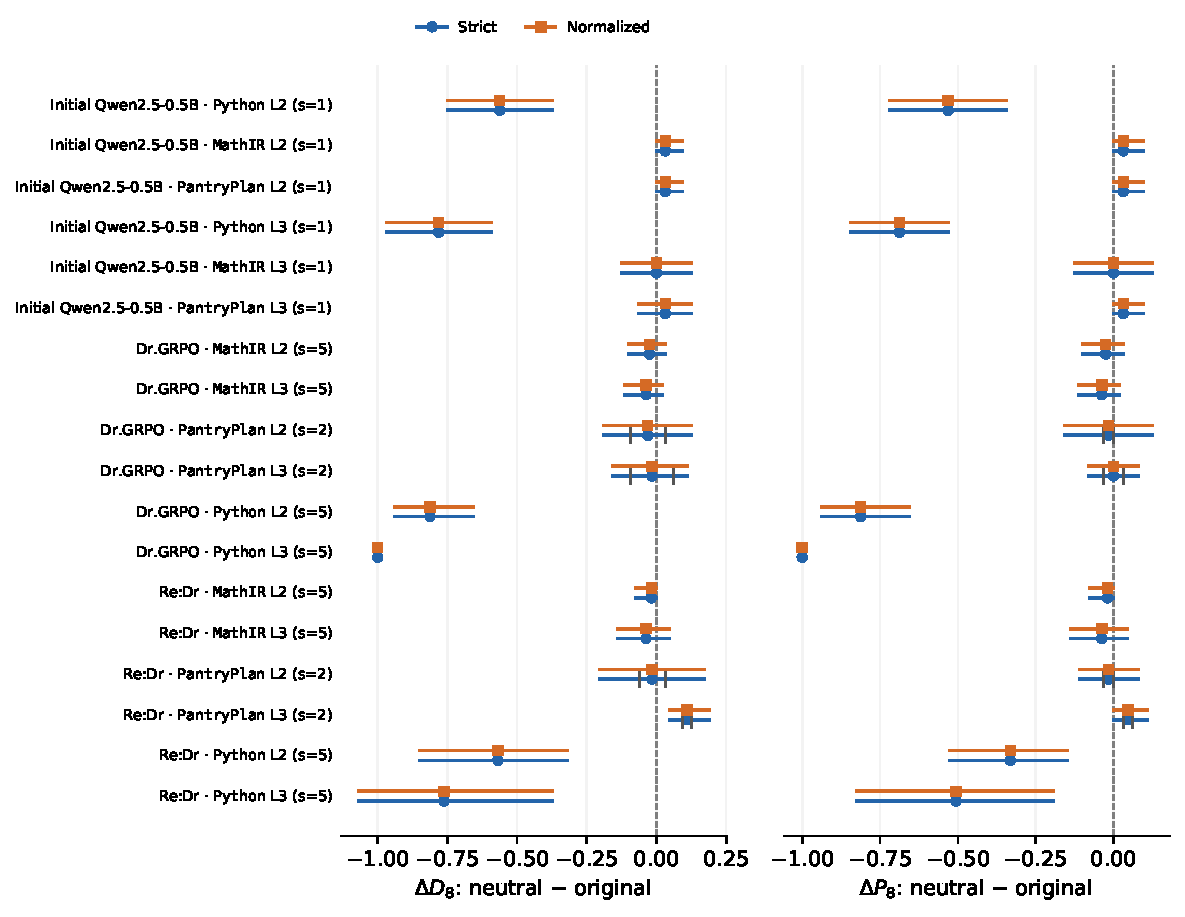
\includegraphics[width=\linewidth]{figures/modebench_prompt_ablation_local.pdf}

\caption{\textbf{\texttt{Python} guidance removal produces the largest wording effects in this panel.} Neutral-minus-original $D_8$ (left) and $P_8$ (right) for the initial Qwen2.5-0.5B checkpoint and Level-2-trained Dr.GRPO and Re:Dr on \texttt{Python}, \texttt{MathIR}, and \texttt{PantryPlan} at Levels 2 and 3, with 32 paired problems and eight draws per arm. Blue circles use strict verification; orange squares use formatting normalization. Horizontal bars are pointwise 95\% bootstrap intervals; the vertical dashed line marks zero. Five-seed groups resample training seeds and paired problems; \texttt{PantryPlan} and initial-model intervals condition on two checkpoints and one checkpoint, respectively. Gray marks show the individual effects for the two \texttt{PantryPlan} training seeds. }

\label{fig:prompt-hints-local}

\end{figure}



\begin{samepage}
\paragraph{Two-seed \texttt{PantryPlan} effects.} Intervals condition on the two checkpoints and do not quantify training-seed variability. The effects for each seed are shown below; each pair gives $(\Delta P_8,\Delta D_8)$.
\begin{center}\small
\begin{tabular}{llcc}
\toprule
Method & Level & First seed & Second seed \\
\midrule
Dr.GRPO & 2 & $(+0.000, +0.03)$ & $(-0.031, -0.09)$ \\
Dr.GRPO & 3 & $(+0.031, +0.06)$ & $(-0.031, -0.09)$ \\
Re:Dr & 2 & $(-0.031, -0.06)$ & $(+0.000, +0.03)$ \\
Re:Dr & 3 & $(+0.031, +0.12)$ & $(+0.062, +0.09)$ \\
\bottomrule
\end{tabular}
\end{center}
\end{samepage}

\paragraph{Scope of the wording intervention.}
The \texttt{Python} intervention removes an executable nested-conditional example
along with divisor-testing and dispatch guidance, and it shortens the prompt.
Its effect concerns this combined change; it does not isolate a preference
cue from example or length effects. Lower \texttt{distinct@8} together with
lower \texttt{pass@8} can reflect reduced correctness rather than increased
concentration among correct outputs. The \pmd{} columns in
Table~\ref{tab:prompt-hints-local-strict} measure conditional diversity on
jointly eligible checkpoint--problem groups. Eligibility itself depends on
correctness, so these comparisons do not hold the full evaluation population
or its accuracy fixed.

\paragraph{Observed prompt dependence.}
\texttt{Python} shows a large loss of correctness after guidance removal. Across the
five Dr.GRPO seeds, mean $P_8$ falls from $.8125$ to zero at Level~2 and from
$1.0$ to zero at Level~3; $D_8$ falls identically and $B_8=0$ in both arms.
With no correct neutral Dr.GRPO outputs, its concentration among correct outputs
is undefined. Re:Dr retains neutral $P_8=.55625$ and $.49375$ and
$D_8=.675$ and $.65625$ at Levels~2 and~3, respectively, while losing
extra verified modes: $\Delta B_8=-.2375$ and $-.25625$. The initial checkpoint
also loses \texttt{Python} correctness (Table~\ref{tab:prompt-hints-local-strict}).
These observations identify substantial dependence on the combined \texttt{Python}
wording intervention; a raw mode-count decline cannot be interpreted solely
as a redistribution among correct answers.


\paragraph{\texttt{Python} responses after hint removal.}
Across 5,120 Dr.GRPO \texttt{Python} responses from five seeds, two levels, and both
wordings, all 2,560 outputs generated with the original wording yield the
same extracted lambda expression, whose body matches the conditional
example in the prompt; 2,320 of these
responses pass verification:
\begin{quote}\footnotesize\ttfamily
lambda n: 2 if n \% 2 == 0 else 3 if n \% 3 == 0 else 5
\end{quote}
\begin{samepage}
Of the 2,560 neutral-wording responses, 1,816 (70.94\%) are invalid Python
expressions, 59 violate other restricted-language rules, 376 return
non-integers, 276 fail the proper-divisor condition, and 33 (1.29\%) have
no extracted candidate after reaching the token limit. Syntax errors are
the largest failure category. The categories follow the first rejection
during extraction, parsing, and execution. They describe output failures
without identifying the training mechanism responsible.

\end{samepage}

\paragraph{Concentration after hint removal.}
Every trained \texttt{MathIR} checkpoint has $B_8=0$ under both wordings at both levels.
Within each problem's eight-draw group, every observed pair of correct
outputs shares a canonical key at every trained checkpoint and level:
correct-pair collision is $1.0$, versus the
uniform reference of $.2$ over five certified modes.
Table~\ref{tab:prompt-hints-local-strict} reports \pmd{} $.000$ under both
wordings in every eligible \texttt{MathIR} comparison. Removing this hint therefore leaves
observed correct outputs concentrated. At Level~2, Re:Dr retains mean $P_8=.975$ without the order hint, compared with $.99375$
with it. Across its five checkpoints, the neutral arm has 4,179 colliding
pairs out of 4,179 correct pairs, from 154 eligible checkpoint--problem
groups; the original arm has 4,382 out of 4,382 pairs from 157 such groups.
Both arms evaluate the same 32 problems at each checkpoint. Thus observed concentration persists after removing the order hint.
The comparison does not measure unseen modes, and the remaining interface
constraints still apply.
\texttt{PantryPlan} effects are mixed. Re:Dr at Level~3 gains $.109375$ in $D_8$,
comprising $.046875$ in $P_8$ and $.0625$ in $B_8$, but this comparison has only
two training seeds. App.~\ref{app:sampling-budget-ablation} evaluates
hosted models under both wordings with 64 draws on sixteen problems per
domain--level combination. Its problem population and sampling budget
differ from the eight-draw evaluation here.


\section{Decoding Temperature, Nucleus, and Budget}
\label{app:decoding-objection}

\paragraph{Temperature at fixed checkpoints.}
Qwen2.5-0.5B Dr.GRPO and Re:Dr checkpoints after eight training passes are
evaluated at $T\in\{.5,.7,1.0,1.3,1.6,2.0\}$, with top-$p=1$ and four
eight-response groups per prompt. Five domains, two methods, and five seeds
give 300 checkpoint--setting evaluations (Fig.~\ref{fig:decoding-objection}A).
The prompt template, evaluation split, response limit, and sampling seeds
are fixed across temperatures. Correct keys are pooled across response
groups for each prompt; the groups have overlapping sampling streams
(App.~\ref{app:conditional-concentration}). Estimates therefore describe
these sampled pools. A seed contributes to the \pmd{} mean when at least
30 prompts yield at least two correct responses. Eligible prompts and seeds
can differ across temperatures and methods.

Across the six temperatures, the largest control \pmd{} is $.021$ in
\texttt{Graph}, $.016$ in \texttt{Countdown}, $.002$ in \texttt{MathIR}, and $.004$ in \texttt{PantryPlan}.
Re:Dr at $T=1$ has corresponding means $.562$, $.485$, $.020$, and $.330$.
These four domains retain five eligible control seeds at every temperature.
\texttt{Python} controls have no seed reaching the 30-prompt threshold, so their
conditional diversity is unidentified under this reporting rule.
The sweep therefore shows low measured control diversity in the four
eligible domains, without establishing that unobserved modes have zero
probability or that every decoding choice would behave the same way.

\paragraph{Hardware sensitivity.}
All evaluations in the temperature sweep use NVIDIA RTX A5000 GPUs.
A paired comparison of A100 and A5000 evaluations at $T=1$ gives mean
absolute \pmd{} difference $.0032$ across twelve comparisons, with maximum
$.0131$. These differences describe the tested hardware comparisons;
they do not bound hardware sensitivity at other checkpoints or settings.

\paragraph{Larger groups and nucleus truncation.}
A separate set of Qwen2.5-0.5B checkpoints trained for twelve passes is evaluated at
eleven settings (Fig.~\ref{fig:decoding-objection}B): the six temperatures
above; two groups of $K=32$ at $T\in\{1.0,1.3,1.6\}$; and four groups
of $K=8$ with top-$p=.95$ at $T\in\{1.0,1.6\}$. The $K=32$ settings
quadruple the group size and double total responses per prompt from 32 to
64. Five domains, two methods, and five seeds give 550 checkpoint--setting
evaluations. The replay variant combines separate mass and within-buffer
balancing terms with novelty and semantic-entropy shaping. Its objective
and training duration therefore differ from the eight-pass Re:Dr comparison.

Control \pmd{} is zero throughout the grid in \texttt{Graph}. Its range is $.006$
to $.031$ in \texttt{Countdown}, $.000$ to $.003$ in \texttt{MathIR}, and $.037$ to $.069$
in \texttt{PantryPlan}.
All eleven settings retain five eligible control seeds in these domains;
\texttt{Python} controls remain below the reporting threshold. The replay markers
provide a descriptive reference for this separate variant, without
identifying the effect of the Re:Dr objective.

Three comparisons hold temperature and nucleus sampling fixed while
increasing both group size and total response budget: $K=8$ and $K=32$ at
$T\in\{1.0,1.3,1.6\}$, top-$p=1$. Across these matched settings, control
\pmd{} changes by at most $.010$ in absolute value, and no
$K=32$ control mean exceeds $.054$. \texttt{Graph} stays at $.000$;
\texttt{Countdown} moves from $.014$--$.027$ to $.013$--$.023$;
\texttt{MathIR} from $.000$--$.001$ to $.001$--$.003$; and \texttt{PantryPlan}
from $.050$--$.063$ to $.045$--$.053$. Each mean uses five eligible seeds.
The larger budget therefore does not move these controls out of their
low-\pmd{} range. This compares sampled pools at fixed checkpoints; it does
not establish that unobserved modes carry zero probability.

\begin{figure}[t]
  \centering
  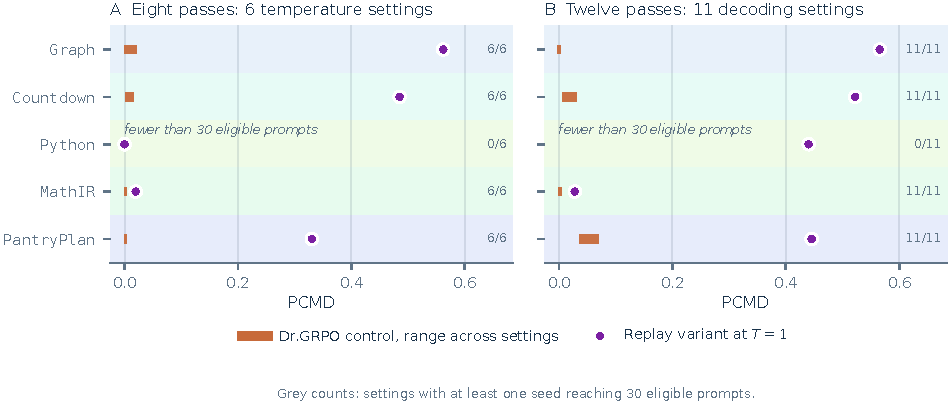
\includegraphics[width=\linewidth]{figures/decoding_objection.pdf}
  \caption{\textbf{Control diversity remains low across the tested decoding
  settings.} Qwen2.5-0.5B terminal \pmd{} across five domains.
  \textbf{(A)} Eight-pass Dr.GRPO/Re:Dr checkpoints at six temperatures
  ($T=.5$--$2.0$): 300 checkpoint--setting evaluations.
  \textbf{(B)} Separate twelve-pass checkpoints at eleven temperature, group-size,
  and nucleus settings: 550 evaluations, using a different replay objective.
  Bars span control means across settings; they are not confidence intervals.
  Markers show the corresponding replay variant at $T=1$, top-$p=1$,
  and $K=8$. Means use seeds with at least 30 prompts having at least two correct
  responses, so control and replay populations need not match. Control bars
  use five seeds outside \texttt{Python}; \texttt{Python} controls have none, while its replay
  markers use two seeds in A and three in B. Counts give eligible settings.
  Ranges narrower than $.004$ are displayed at width $.004$ for visibility.}
  \label{fig:decoding-objection}
\end{figure}

\paragraph{Scope of the decoding comparison.}
Both grids evaluate fixed terminal policies at one model scale. They do not
measure the effects of changing rollout temperature, optimizer settings, or
training duration. Correctness and conditional eligibility can change with
decoding settings; a missing \pmd{} estimate indicates insufficient eligible
prompts, rather than disappearance of all correct solution modes.

\section{Sampling-Budget Ablation}
\label{app:sampling-budget-ablation}

\subsection{Sampling design and estimands}
\label{sec:discovery-curves}
Large-budget \texttt{pass@k} evaluation can reveal differences hidden at smaller budgets \citep{yue2025rlvrlimit}. We evaluate sixteen problems from each of \texttt{Python}, \texttt{MathIR}, and \texttt{PantryPlan} at Levels~2 and~3.

Problems are selected independently of model outputs from the prompt-hint ablation population. Each has original and neutral wordings, with 64 responses per wording from each checkpoint or deployment. Eight-draw estimates use subsets of these same response pools. The initial Qwen2.5-0.5B-Instruct checkpoint has no training-seed replication. Dr.GRPO and Re:Dr use five matched seeds in \texttt{Python} and \texttt{MathIR} and two in \texttt{PantryPlan}. These checkpoints are trained at Level~2, so Level~3 measures transfer.

For a 64-draw pool, let $c$ be the number of correct outputs and $n_j$ the count of verified canonical key $j$. At $k\in\{1,2,4,8,16,32,64\}$, we average over all size-$k$ subsets without replacement:
\[
 P_k=1-\frac{\binom{64-c}{k}}{\binom{64}{k}},\qquad
 D_k=\sum_j\left[1-\frac{\binom{64-n_j}{k}}{\binom{64}{k}}\right],\qquad B_k=D_k-P_k.
\]
Here $P_k$ is the probability of at least one correct response, $D_k$ is the expected number of distinct verified modes, and $B_k$ is the expected number of modes beyond the first success. Infeasible numerator combinations are zero. Incorrect, empty, refused, and truncated responses remain in the pool; only verifier-accepted responses contribute keys. The curve points are correlated because they share a response pool and describe finite-sample discovery. The gains $G_P=P_{64}-P_8$, $G_D=D_{64}-D_8$, and $G_B=B_{64}-B_8$ distinguish improvements in first-success probability from the discovery of additional modes; they do not estimate complete unseen support.

We report strict-verifier results and a formatting-normalization sensitivity analysis that preserves every strict success and canonical key. Intervals use 20,000 whole-problem bootstrap replicates, paired across wordings and stratified by domain and level. Five-seed intervals also resample matched training seeds with shared problem indices; \texttt{PantryPlan} intervals condition on its two checkpoints. Each domain--level comparison contains sixteen problems, and intervals are unadjusted for multiple comparisons. Zero-width intervals indicate no observed resampled variation and do not establish equivalence.

For breadth at a fixed number of correct draws, we average over subsets of $m$ correct responses:
\[
 R_m=\sum_j\left[1-\frac{\binom{c-n_j}{m}}{\binom{c}{m}}\right].
\]
Paired comparisons require $c\ge m$ under both wordings. They therefore condition on observed success, without equating accuracy or estimating diversity for excluded problems.

Eligibility varies with $m$, method, and grading. Trained-checkpoint means weight seeds equally and are undefined if any seed lacks eligible prompts. Conditional intervals retain only bootstrap replicates in which the corresponding mean is defined.

The 64-draw summaries use two prompt weightings. Pooled collision $C$ divides the total number of equal-key correct pairs by the total number of correct pairs within each checkpoint or deployment; a prompt therefore receives weight proportional to $\binom{c}{2}$. Promptwise \pmd{} averages $1-\sum_j\binom{n_j}{2}/\binom{c}{2}$ equally over prompts with $c\ge2$. Each wording's absolute estimate uses its own eligible prompts, whereas the neutral-minus-original contrast $\Delta\pmd$ uses only jointly eligible prompts. Trained-checkpoint estimates then receive equal weight across seeds.

Support references use certified lower bounds $L\le M$: two valid modes in \texttt{Python}, five in \texttt{MathIR}, and the problem-specific certificate count in \texttt{PantryPlan}. Thus $1/L$ is an upper reference for collision under a uniform distribution over full support, and $L[1-(1-1/L)^m]$ is a lower reference for uniform expected breadth. These references describe uniform sampling; they do not bound model breadth, and observed distinct counts may exceed $L$.

In the tables, O/N denotes original/neutral wording, and $\Delta G_D$ is the neutral-minus-original discovery gain. $U$ denotes the uniform reference under the corresponding weighting. $E_O/E_N$ count separately eligible checkpoint--problem pairs with $c\ge2$; $Q_O/Q_N$ count correct response pairs. The counts sum across checkpoints, whereas the estimates weight checkpoints equally. Separate eligibility counts do not give the size of the jointly eligible population used for a contrast.


\begin{table}[!htbp]
\centering\scriptsize
\setlength{\tabcolsep}{3pt}
\caption{\textbf{Discovery gains from eight to 64 draws.} Strict verification; O/N denotes original/neutral wording. Each row reports sixteen problems for one deployment, domain, and level. Intervals resample paired problems, with no replication across model training seeds.}
\label{tab:discovery-gains-frontier-strict}
\resizebox{\linewidth}{!}{%
\begin{tabular}{llrrrr}
\toprule
Model & Domain/level & $G_P$: O/N & $G_D$: O/N & $G_B$: O/N & $\Delta G_D$ [95\%] \\
\midrule
GPT-5.4 & \texttt{Python} L2 & $0.014/0.000$ & $2.017/3.051$ & $2.003/3.051$ & $+1.033\;[-0.044,+2.371]$ \\
GPT-5.6 Sol & \texttt{Python} L2 & $0.000/0.405$ & $0.000/0.866$ & $0.000/0.462$ & $+0.866\;[+0.545,+1.231]$ \\
Grok 4.3 & \texttt{Python} L2 & $0.000/0.000$ & $0.667/1.013$ & $0.667/1.013$ & $+0.346\;[-0.583,+1.128]$ \\
GPT-5.4 & \texttt{Python} L3 & $0.025/0.000$ & $2.100/2.340$ & $2.076/2.340$ & $+0.240\;[-0.379,+0.930]$ \\
GPT-5.6 Sol & \texttt{Python} L3 & $0.000/0.586$ & $0.000/0.759$ & $0.000/0.174$ & $+0.759\;[+0.581,+0.952]$ \\
Grok 4.3 & \texttt{Python} L3 & $0.000/0.000$ & $0.424/1.576$ & $0.424/1.576$ & $+1.152\;[+0.640,+1.689]$ \\
GPT-5.4 & \texttt{MathIR} L2 & $0.043/0.042$ & $0.043/0.909$ & $0.000/0.868$ & $+0.867\;[+0.587,+1.111]$ \\
GPT-5.6 Sol & \texttt{MathIR} L2 & $0.027/0.004$ & $0.027/0.686$ & $0.000/0.682$ & $+0.659\;[+0.416,+0.888]$ \\
Grok 4.3 & \texttt{MathIR} L2 & $0.000/0.001$ & $0.223/0.322$ & $0.223/0.321$ & $+0.099\;[-0.226,+0.438]$ \\
GPT-5.4 & \texttt{MathIR} L3 & $0.000/0.000$ & $0.055/0.663$ & $0.055/0.663$ & $+0.609\;[+0.342,+0.888]$ \\
GPT-5.6 Sol & \texttt{MathIR} L3 & $0.000/0.000$ & $0.000/0.515$ & $0.000/0.515$ & $+0.515\;[+0.318,+0.714]$ \\
Grok 4.3 & \texttt{MathIR} L3 & $0.000/0.000$ & $0.167/0.805$ & $0.167/0.805$ & $+0.638\;[+0.348,+0.935]$ \\
GPT-5.4 & \texttt{PantryPlan} L2 & $0.001/0.015$ & $1.158/2.583$ & $1.156/2.568$ & $+1.426\;[+0.423,+2.641]$ \\
GPT-5.6 Sol & \texttt{PantryPlan} L2 & $0.086/0.101$ & $0.917/1.789$ & $0.831/1.688$ & $+0.872\;[+0.245,+1.575]$ \\
Grok 4.3 & \texttt{PantryPlan} L2 & $0.000/0.000$ & $1.022/3.377$ & $1.022/3.377$ & $+2.354\;[+1.592,+3.123]$ \\
GPT-5.4 & \texttt{PantryPlan} L3 & $0.000/0.002$ & $1.666/3.219$ & $1.666/3.218$ & $+1.553\;[+0.776,+2.367]$ \\
GPT-5.6 Sol & \texttt{PantryPlan} L3 & $0.032/0.129$ & $1.625/1.842$ & $1.592/1.713$ & $+0.217\;[-0.489,+0.921]$ \\
Grok 4.3 & \texttt{PantryPlan} L3 & $0.000/0.000$ & $1.810/4.466$ & $1.810/4.466$ & $+2.656\;[+1.698,+3.640]$ \\
\bottomrule
\end{tabular}}
\end{table}

\begin{table}[!htbp]
\centering\scriptsize
\setlength{\tabcolsep}{3pt}
\caption{\textbf{Discovery gains from eight to 64 draws.} Formatting normalization; O/N denotes original/neutral wording. Each row reports sixteen problems for one deployment, domain, and level. Intervals resample paired problems, with no replication across model training seeds.}
\label{tab:discovery-gains-frontier-normalized-secondary}
\resizebox{\linewidth}{!}{%
\begin{tabular}{llrrrr}
\toprule
Model & Domain/level & $G_P$: O/N & $G_D$: O/N & $G_B$: O/N & $\Delta G_D$ [95\%] \\
\midrule
GPT-5.4 & \texttt{Python} L2 & $0.000/0.000$ & $2.156/3.216$ & $2.156/3.216$ & $+1.060\;[-0.071,+2.386]$ \\
GPT-5.6 Sol & \texttt{Python} L2 & $0.008/0.010$ & $0.113/0.794$ & $0.105/0.784$ & $+0.681\;[+0.351,+1.066]$ \\
Grok 4.3 & \texttt{Python} L2 & $0.000/0.000$ & $0.667/1.013$ & $0.667/1.013$ & $+0.346\;[-0.583,+1.128]$ \\
GPT-5.4 & \texttt{Python} L3 & $0.000/0.000$ & $2.431/2.604$ & $2.431/2.604$ & $+0.173\;[-0.657,+1.075]$ \\
GPT-5.6 Sol & \texttt{Python} L3 & $0.011/0.007$ & $0.120/0.490$ & $0.109/0.483$ & $+0.370\;[+0.112,+0.674]$ \\
Grok 4.3 & \texttt{Python} L3 & $0.000/0.000$ & $0.424/1.576$ & $0.424/1.576$ & $+1.152\;[+0.640,+1.689]$ \\
GPT-5.4 & \texttt{MathIR} L2 & $0.043/0.042$ & $0.043/0.909$ & $0.000/0.868$ & $+0.867\;[+0.587,+1.111]$ \\
GPT-5.6 Sol & \texttt{MathIR} L2 & $0.027/0.004$ & $0.027/0.686$ & $0.000/0.682$ & $+0.659\;[+0.416,+0.888]$ \\
Grok 4.3 & \texttt{MathIR} L2 & $0.000/0.001$ & $0.223/0.322$ & $0.223/0.321$ & $+0.099\;[-0.226,+0.438]$ \\
GPT-5.4 & \texttt{MathIR} L3 & $0.000/0.000$ & $0.055/0.663$ & $0.055/0.663$ & $+0.609\;[+0.342,+0.888]$ \\
GPT-5.6 Sol & \texttt{MathIR} L3 & $0.000/0.000$ & $0.000/0.515$ & $0.000/0.515$ & $+0.515\;[+0.318,+0.714]$ \\
Grok 4.3 & \texttt{MathIR} L3 & $0.000/0.000$ & $0.167/0.805$ & $0.167/0.805$ & $+0.638\;[+0.348,+0.935]$ \\
GPT-5.4 & \texttt{PantryPlan} L2 & $0.001/0.015$ & $1.158/2.583$ & $1.156/2.568$ & $+1.426\;[+0.423,+2.641]$ \\
GPT-5.6 Sol & \texttt{PantryPlan} L2 & $0.004/0.004$ & $0.954/1.834$ & $0.950/1.830$ & $+0.880\;[+0.237,+1.547]$ \\
Grok 4.3 & \texttt{PantryPlan} L2 & $0.000/0.000$ & $1.022/3.377$ & $1.022/3.377$ & $+2.354\;[+1.592,+3.123]$ \\
GPT-5.4 & \texttt{PantryPlan} L3 & $0.000/0.002$ & $1.666/3.219$ & $1.666/3.218$ & $+1.553\;[+0.776,+2.367]$ \\
GPT-5.6 Sol & \texttt{PantryPlan} L3 & $0.001/0.020$ & $1.586/2.462$ & $1.585/2.443$ & $+0.877\;[+0.272,+1.436]$ \\
Grok 4.3 & \texttt{PantryPlan} L3 & $0.000/0.000$ & $1.810/4.466$ & $1.810/4.466$ & $+2.656\;[+1.698,+3.640]$ \\
\bottomrule
\end{tabular}}
\end{table}

\begin{figure}[!htbp]

\centering

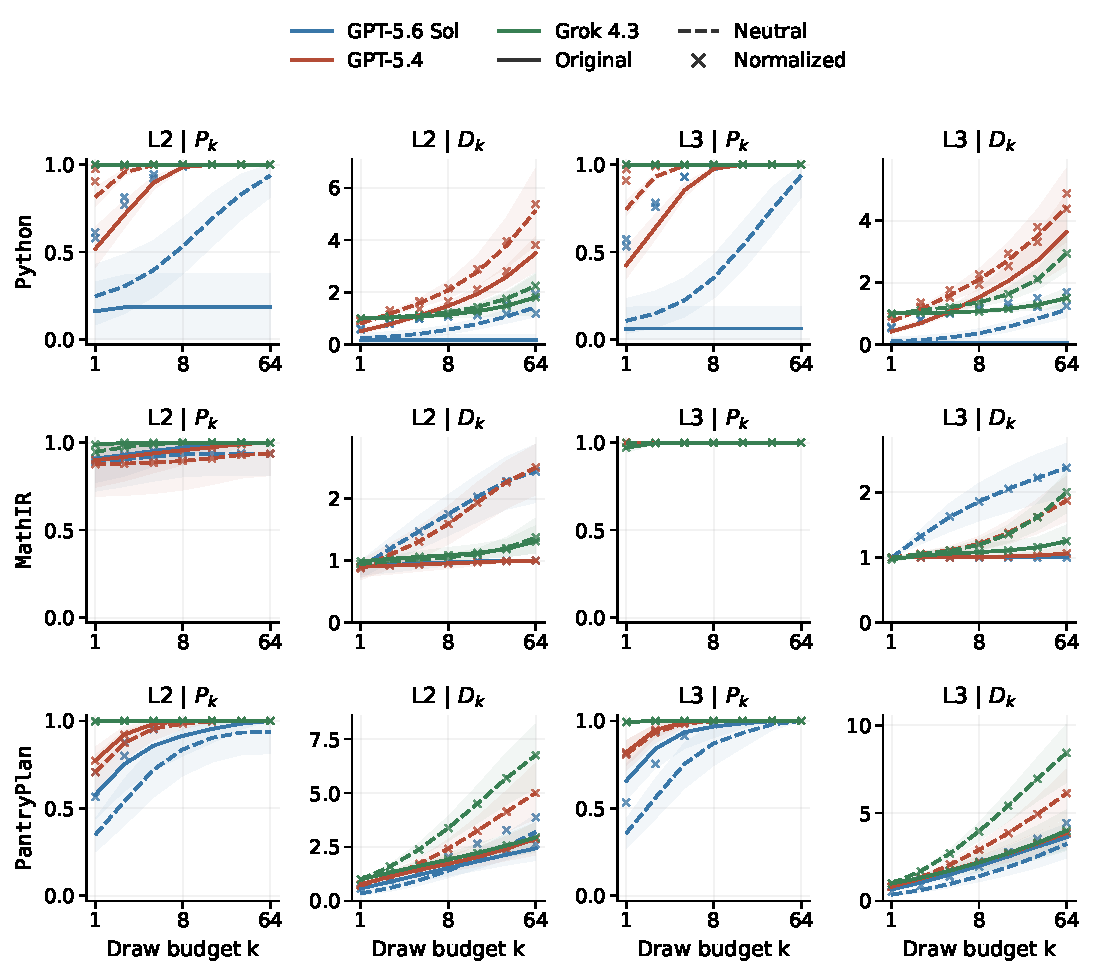
\includegraphics[width=\linewidth,height=0.72\textheight,keepaspectratio]{figures/modebench_discovery_curves_frontier.pdf}

\caption{\textbf{Additional draws reveal solution modes beyond early success.} Hosted deployments; rows show \texttt{Python}, \texttt{MathIR}, and \texttt{PantryPlan}, with paired $P_k$ and $D_k$ columns for Levels~2 and~3. Curves show pass probability $P_k$ and distinct verified modes $D_k$ against draw budget $k$, obtained by averaging over size-$k$ subsets within sixteen 64-draw problem pools per domain and level. Colours identify deployments; solid/dashed lines denote original/neutral wording. Lines use strict verification, crosses formatting normalization, and shading pointwise 95\% bootstrap intervals. Intervals resample paired problems within each domain and level and condition on the deployment.}

\label{fig:discovery-curves-frontier}

\end{figure}

\begin{table}[!htbp]
\centering\scriptsize
\setlength{\tabcolsep}{3pt}
\caption{\textbf{Pair weighting changes the summary of correct-solution diversity.} Strict 64-draw estimates for hosted deployments. Collision $C$ weights prompts by their number of correct pairs; \pmd{} weights eligible prompts equally. Absolute estimates for each wording use their own eligible prompts, whereas $\Delta\pmd$ uses only jointly eligible prompts. Thus $\Delta\pmd$ need not equal the difference between the displayed absolute estimates, and $E_O/E_N$ are separate eligibility counts. Each deployment is fixed; intervals resample paired problems.}
\label{tab:discovery-breadth-frontier}
\resizebox{\linewidth}{!}{%
\begin{tabular}{llrrrrrrrrr}
\toprule
Model & Domain/level & $C_O$ & $C_N$ & $\pmd_O$ & $\pmd_N$ & $U^{C}_O$ & $U^{\pmd}_O$ & $E_O/E_N$ & $Q_O/Q_N$ & $\Delta\pmd$ [95\%] \\
\midrule
GPT-5.4 & \texttt{Python} L2 & $0.790$ & $0.665$ & $0.257$ & $0.341$ & $0.500$ & $0.500$ & 16/16 & 10374/21720 & $+0.084\;[-0.006,+0.186]$ \\
GPT-5.6 Sol & \texttt{Python} L2 & $1.000$ & $0.974$ & $0.000$ & $0.184$ & $0.500$ & $0.500$ & 3/13 & 4467/6074 & $+0.021\;[+0.000,+0.032]$ \\
Grok 4.3 & \texttt{Python} L2 & $0.963$ & $0.938$ & $0.037$ & $0.062$ & $0.500$ & $0.500$ & 16/16 & 32256/32256 & $+0.025\;[+0.002,+0.048]$ \\
GPT-5.4 & \texttt{Python} L3 & $0.732$ & $0.620$ & $0.334$ & $0.384$ & $0.500$ & $0.500$ & 16/16 & 6747/18043 & $+0.050\;[-0.026,+0.128]$ \\
GPT-5.6 Sol & \texttt{Python} L3 & $1.000$ & $0.966$ & $0.000$ & $0.130$ & $0.500$ & $0.500$ & 1/10 & 1953/2097 & $+0.031\;[+0.031,+0.031]$ \\
Grok 4.3 & \texttt{Python} L3 & $0.981$ & $0.893$ & $0.019$ & $0.107$ & $0.500$ & $0.500$ & 16/16 & 32193/32256 & $+0.087\;[+0.041,+0.154]$ \\
GPT-5.4 & \texttt{MathIR} L2 & $1.000$ & $0.756$ & $0.000$ & $0.228$ & $0.200$ & $0.800$ & 16/15 & 28440/28227 & $+0.228\;[+0.161,+0.302]$ \\
GPT-5.6 Sol & \texttt{MathIR} L2 & $1.000$ & $0.678$ & $0.000$ & $0.302$ & $0.200$ & $0.800$ & 16/15 & 28645/28377 & $+0.302\;[+0.200,+0.402]$ \\
Grok 4.3 & \texttt{MathIR} L2 & $0.968$ & $0.985$ & $0.033$ & $0.014$ & $0.200$ & $0.800$ & 16/16 & 31600/29677 & $-0.020\;[-0.076,+0.017]$ \\
GPT-5.4 & \texttt{MathIR} L3 & $0.998$ & $0.944$ & $0.002$ & $0.056$ & $0.200$ & $0.800$ & 16/16 & 32256/32256 & $+0.054\;[+0.027,+0.087]$ \\
GPT-5.6 Sol & \texttt{MathIR} L3 & $1.000$ & $0.676$ & $0.000$ & $0.324$ & $0.200$ & $0.800$ & 16/16 & 32256/32256 & $+0.324\;[+0.208,+0.432]$ \\
Grok 4.3 & \texttt{MathIR} L3 & $0.966$ & $0.949$ & $0.033$ & $0.051$ & $0.200$ & $0.800$ & 16/16 & 30520/32193 & $+0.019\;[-0.046,+0.064]$ \\
GPT-5.4 & \texttt{PantryPlan} L2 & $0.680$ & $0.499$ & $0.252$ & $0.483$ & $0.069$ & $0.934$ & 16/16 & 20097/17436 & $+0.231\;[+0.069,+0.395]$ \\
GPT-5.6 Sol & \texttt{PantryPlan} L2 & $0.674$ & $0.624$ & $0.275$ & $0.474$ & $0.076$ & $0.934$ & 16/15 & 12941/5001 & $+0.180\;[+0.058,+0.327]$ \\
Grok 4.3 & \texttt{PantryPlan} L2 & $0.684$ & $0.412$ & $0.315$ & $0.589$ & $0.066$ & $0.934$ & 16/16 & 32005/32193 & $+0.274\;[+0.143,+0.411]$ \\
GPT-5.4 & \texttt{PantryPlan} L3 & $0.546$ & $0.392$ & $0.431$ & $0.610$ & $0.065$ & $0.937$ & 16/16 & 22332/21975 & $+0.179\;[+0.103,+0.257]$ \\
GPT-5.6 Sol & \texttt{PantryPlan} L3 & $0.566$ & $0.652$ & $0.422$ & $0.441$ & $0.061$ & $0.937$ & 16/16 & 15229/4946 & $+0.019\;[-0.136,+0.172]$ \\
Grok 4.3 & \texttt{PantryPlan} L3 & $0.673$ & $0.294$ & $0.330$ & $0.703$ & $0.063$ & $0.937$ & 16/16 & 31830/31881 & $+0.373\;[+0.224,+0.523]$ \\
\bottomrule
\end{tabular}}
\end{table}

\begin{figure}[!htbp]

\centering

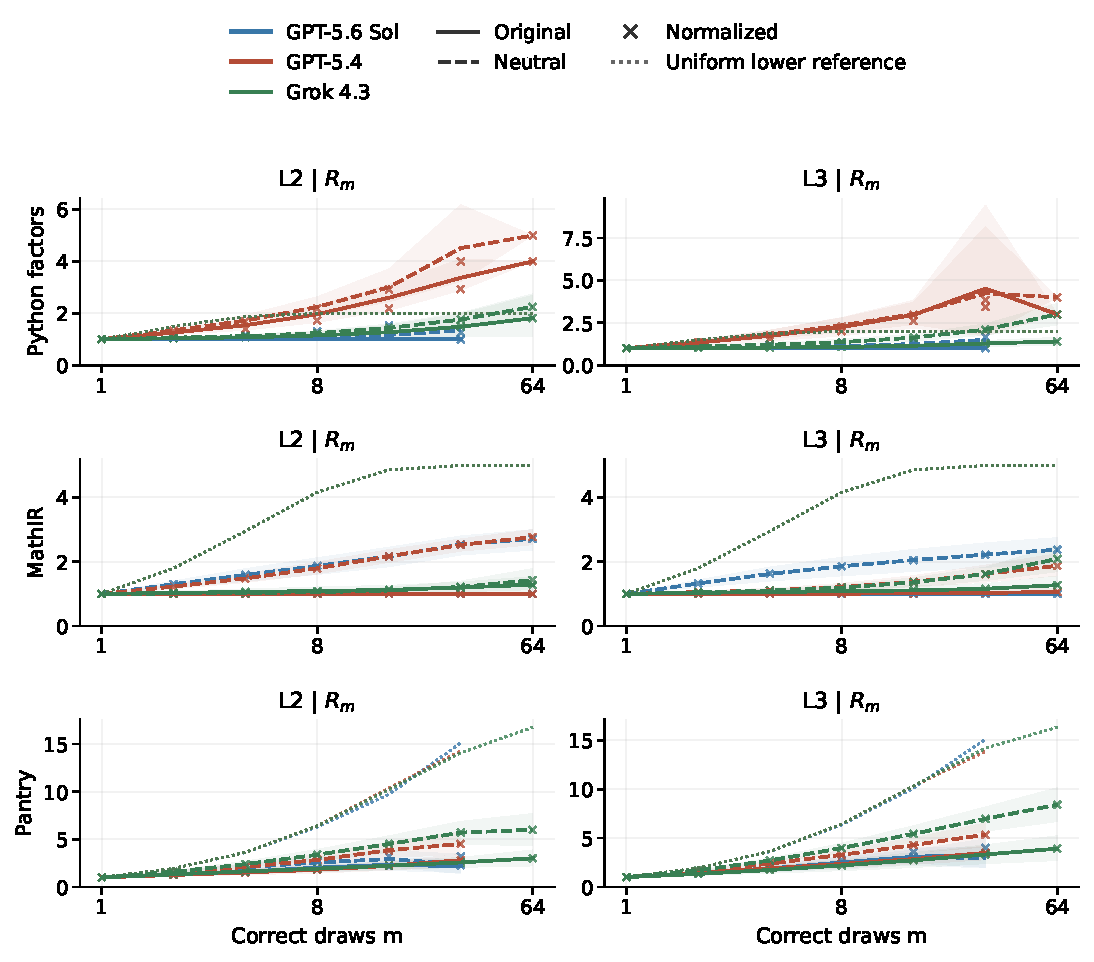
\includegraphics[width=\linewidth,height=0.66\textheight,keepaspectratio]{figures/modebench_discovery_correct_budget_frontier.pdf}

\caption{\textbf{Neutral wording broadens GPT solutions in \texttt{MathIR} at fixed correct-draw budgets.} Hosted deployments; rows show \texttt{Python}, \texttt{MathIR}, and \texttt{PantryPlan}, and columns Levels~2 and~3. Curves show $R_m$, the expected number of distinct verified modes in $m$ correct draws, on prompts with at least $m$ correct outputs under both wordings. Eligibility varies with $m$, method, and grading; gaps mark undefined means. Dotted lines give uniform lower references on prompts eligible under strict grading in both wordings, with the same prompt and checkpoint weighting as the strict curves. Colours identify deployments; solid/dashed lines denote original/neutral wording. Lines use strict verification, crosses formatting normalization, and shading pointwise 95\% bootstrap intervals. Intervals resample paired problems within each domain and level and condition on the deployment.}

\label{fig:discovery-correct-budget-frontier}

\end{figure}

\begin{table}[!htbp]
\centering\scriptsize
\setlength{\tabcolsep}{3pt}
\caption{\textbf{Discovery gains from eight to 64 draws.} Strict verification; O/N denotes original/neutral wording. Qwen2.5-0.5B-Instruct checkpoint means use five training seeds in \texttt{Python} and \texttt{MathIR} and two in \texttt{PantryPlan}; $s=1$ denotes the single initial checkpoint. Five-seed intervals resample seeds and paired prompts; \texttt{PantryPlan} intervals condition on its two checkpoints. Formatting normalization leaves every Qwen estimate unchanged.}
\label{tab:discovery-gains-local-strict}
\resizebox{\linewidth}{!}{%
\begin{tabular}{llrrrr}
\toprule
Model & Domain/level & $G_P$: O/N & $G_D$: O/N & $G_B$: O/N & $\Delta G_D$ [95\%] \\
\midrule
Dr.GRPO ($s=5$) & \texttt{Python} L2 & $0.000/0.000$ & $0.000/0.000$ & $0.000/0.000$ & $+0.000\;[+0.000,+0.000]$ \\
Initial ($s=1$) & \texttt{Python} L2 & $0.147/0.105$ & $0.303/0.165$ & $0.156/0.060$ & $-0.138\;[-0.217,-0.061]$ \\
Re:Dr ($s=5$) & \texttt{Python} L2 & $0.000/0.231$ & $0.058/0.463$ & $0.058/0.232$ & $+0.405\;[+0.185,+0.620]$ \\
Dr.GRPO ($s=5$) & \texttt{Python} L3 & $0.000/0.033$ & $0.000/0.033$ & $0.000/0.000$ & $+0.033\;[+0.000,+0.120]$ \\
Initial ($s=1$) & \texttt{Python} L3 & $0.218/0.096$ & $0.593/0.096$ & $0.376/0.000$ & $-0.497\;[-0.766,-0.270]$ \\
Re:Dr ($s=5$) & \texttt{Python} L3 & $0.000/0.239$ & $0.153/0.531$ & $0.153/0.292$ & $+0.379\;[+0.111,+0.678]$ \\
Dr.GRPO ($s=5$) & \texttt{MathIR} L2 & $0.021/0.017$ & $0.021/0.017$ & $0.000/0.000$ & $-0.004\;[-0.068,+0.045]$ \\
Initial ($s=1$) & \texttt{MathIR} L2 & $0.344/0.235$ & $0.344/0.235$ & $0.000/0.000$ & $-0.109\;[-0.383,+0.164]$ \\
Re:Dr ($s=5$) & \texttt{MathIR} L2 & $0.010/0.011$ & $0.010/0.011$ & $0.000/0.000$ & $+0.001\;[-0.036,+0.050]$ \\
Dr.GRPO ($s=5$) & \texttt{MathIR} L3 & $0.023/0.018$ & $0.026/0.018$ & $0.004/0.000$ & $-0.008\;[-0.065,+0.038]$ \\
Initial ($s=1$) & \texttt{MathIR} L3 & $0.254/0.246$ & $0.359/0.360$ & $0.105/0.114$ & $+0.001\;[-0.123,+0.095]$ \\
Re:Dr ($s=5$) & \texttt{MathIR} L3 & $0.064/0.056$ & $0.064/0.056$ & $0.000/0.000$ & $-0.008\;[-0.099,+0.059]$ \\
Dr.GRPO ($s=2$) & \texttt{PantryPlan} L2 & $0.332/0.323$ & $0.718/0.736$ & $0.386/0.414$ & $+0.018\;[-0.422,+0.433]$ \\
Initial ($s=1$) & \texttt{PantryPlan} L2 & $0.440/0.419$ & $0.857/0.955$ & $0.416/0.537$ & $+0.099\;[-0.201,+0.392]$ \\
Re:Dr ($s=2$) & \texttt{PantryPlan} L2 & $0.141/0.147$ & $0.415/0.429$ & $0.274/0.282$ & $+0.014\;[-0.123,+0.152]$ \\
Dr.GRPO ($s=2$) & \texttt{PantryPlan} L3 & $0.268/0.258$ & $0.949/1.025$ & $0.681/0.766$ & $+0.076\;[-0.237,+0.465]$ \\
Initial ($s=1$) & \texttt{PantryPlan} L3 & $0.259/0.384$ & $0.927/1.078$ & $0.668/0.694$ & $+0.151\;[-0.109,+0.399]$ \\
Re:Dr ($s=2$) & \texttt{PantryPlan} L3 & $0.204/0.149$ & $0.568/0.461$ & $0.364/0.312$ & $-0.107\;[-0.321,+0.098]$ \\
\bottomrule
\end{tabular}}
\end{table}

\begin{figure}[!htbp]

\centering

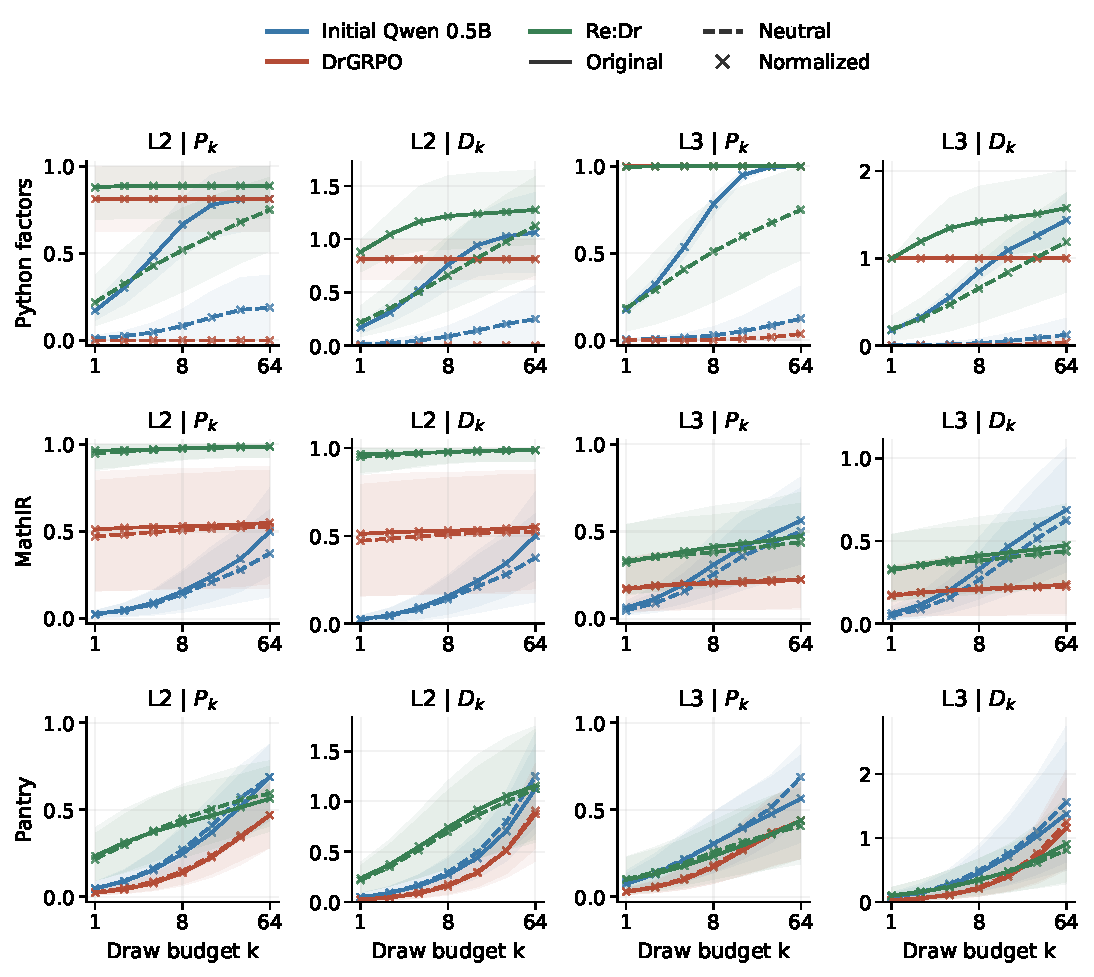
\includegraphics[width=\linewidth,height=0.72\textheight,keepaspectratio]{figures/modebench_discovery_curves_local.pdf}

\caption{\textbf{Additional draws reveal few new \texttt{MathIR} modes after training.} Qwen2.5-0.5B-Instruct checkpoints; rows show \texttt{Python}, \texttt{MathIR}, and \texttt{PantryPlan}, with paired $P_k$ and $D_k$ columns for Levels~2 and~3. Curves show pass probability $P_k$ and distinct verified modes $D_k$ against draw budget $k$, obtained by averaging over size-$k$ subsets within sixteen 64-draw problem pools per domain and level. Colours identify methods; solid/dashed lines denote original/neutral wording. Lines use strict verification, crosses formatting normalization, and shading pointwise 95\% bootstrap intervals. Means weight checkpoints equally: five training seeds in \texttt{Python} and \texttt{MathIR}, two in \texttt{PantryPlan}, and one initial checkpoint. Five-seed intervals resample seeds and paired problems; \texttt{PantryPlan} and initial intervals condition on the observed checkpoints for each method.}

\label{fig:discovery-curves-local}

\end{figure}

\begin{table}[!htbp]
\centering\scriptsize
\setlength{\tabcolsep}{3pt}
\caption{\textbf{Pair weighting changes the summary of correct-solution diversity.} Strict 64-draw estimates for Qwen2.5-0.5B-Instruct checkpoints. Collision $C$ weights prompts by their number of correct pairs; \pmd{} weights eligible prompts equally. Absolute estimates for each wording use their own eligible prompts, whereas $\Delta\pmd$ uses only jointly eligible prompts. Thus $\Delta\pmd$ need not equal the difference between the displayed absolute estimates, and $E_O/E_N$ are separate eligibility counts. Means weight checkpoints equally and are undefined if any seed lacks eligible prompts.}
\label{tab:discovery-breadth-local}
\resizebox{\linewidth}{!}{%
\begin{tabular}{llrrrrrrrrr}
\toprule
Model & Domain/level & $C_O$ & $C_N$ & $\pmd_O$ & $\pmd_N$ & $U^{C}_O$ & $U^{\pmd}_O$ & $E_O/E_N$ & $Q_O/Q_N$ & $\Delta\pmd$ [95\%] \\
\midrule
Dr.GRPO & \texttt{Python} L2 & $1.000$ & $--$ & $0.000$ & $--$ & $0.500$ & $0.500$ & 65/0 & 130977/0 & $--$ \\
Initial & \texttt{Python} L2 & $0.791$ & $0.875$ & $0.097$ & $0.167$ & $0.500$ & $0.500$ & 13/3 & 1270/24 & $-0.252\;[-0.395,+0.019]$ \\
Re:Dr & \texttt{Python} L2 & $0.809$ & $0.800$ & $0.191$ & $0.156$ & $0.500$ & $0.500$ & 71/53 & 140722/18289 & $-0.037\;[-0.139,+0.037]$ \\
Dr.GRPO & \texttt{Python} L3 & $1.000$ & $--$ & $0.000$ & $--$ & $0.500$ & $0.500$ & 80/0 & 161280/0 & $--$ \\
Initial & \texttt{Python} L3 & $0.875$ & $1.000$ & $0.101$ & $0.000$ & $0.500$ & $0.500$ & 16/1 & 1010/3 & $-0.513\;[-0.513,-0.513]$ \\
Re:Dr & \texttt{Python} L3 & $0.805$ & $0.797$ & $0.195$ & $0.227$ & $0.500$ & $0.500$ & 80/52 & 160275/12893 & $+0.030\;[-0.023,+0.117]$ \\
Dr.GRPO & \texttt{MathIR} L2 & $1.000$ & $1.000$ & $0.000$ & $0.000$ & $0.200$ & $0.800$ & 43/42 & 80766/74119 & $+0.000\;[+0.000,+0.000]$ \\
Initial & \texttt{MathIR} L2 & $1.000$ & $1.000$ & $0.000$ & $0.000$ & $0.200$ & $0.800$ & 3/3 & 64/64 & $+0.000\;[+0.000,+0.000]$ \\
Re:Dr & \texttt{MathIR} L2 & $1.000$ & $1.000$ & $0.000$ & $0.000$ & $0.200$ & $0.800$ & 79/79 & 155016/151485 & $+0.000\;[+0.000,+0.000]$ \\
Dr.GRPO & \texttt{MathIR} L3 & $0.980$ & $1.000$ & $0.038$ & $0.000$ & $0.200$ & $0.800$ & 16/18 & 24457/25393 & $-0.038\;[-0.202,+0.000]$ \\
Initial & \texttt{MathIR} L3 & $0.883$ & $0.912$ & $0.128$ & $0.162$ & $0.200$ & $0.800$ & 7/6 & 282/181 & $+0.013\;[-0.014,+0.052]$ \\
Re:Dr & \texttt{MathIR} L3 & $1.000$ & $1.000$ & $0.000$ & $0.000$ & $0.200$ & $0.800$ & 34/34 & 46891/50301 & $+0.000\;[+0.000,+0.000]$ \\
Dr.GRPO & \texttt{PantryPlan} L2 & $0.374$ & $0.276$ & $0.733$ & $0.780$ & $0.047$ & $0.953$ & 9/10 & 101/193 & $+0.220\;[-0.030,+0.470]$ \\
Initial & \texttt{PantryPlan} L2 & $0.849$ & $0.787$ & $0.587$ & $0.623$ & $0.052$ & $0.945$ & 7/10 & 212/178 & $-0.078\;[-0.300,+0.064]$ \\
Re:Dr & \texttt{PantryPlan} L2 & $0.600$ & $0.613$ & $0.343$ & $0.218$ & $0.051$ & $0.942$ & 16/18 & 10144/8510 & $-0.093\;[-0.220,+0.007]$ \\
Dr.GRPO & \texttt{PantryPlan} L3 & $0.203$ & $0.228$ & $0.808$ & $0.680$ & $0.047$ & $0.950$ & 10/12 & 134/165 & $-0.156\;[-0.359,+0.081]$ \\
Initial & \texttt{PantryPlan} L3 & $0.375$ & $0.313$ & $0.307$ & $0.341$ & $0.049$ & $0.945$ & 7/6 & 531/705 & $-0.017\;[-0.109,+0.091]$ \\
Re:Dr & \texttt{PantryPlan} L3 & $0.636$ & $0.666$ & $0.337$ & $0.198$ & $0.051$ & $0.941$ & 10/11 & 4006/3946 & $-0.112\;[-0.319,+0.008]$ \\
\bottomrule
\end{tabular}}
\end{table}

\begin{figure}[!htbp]

\centering

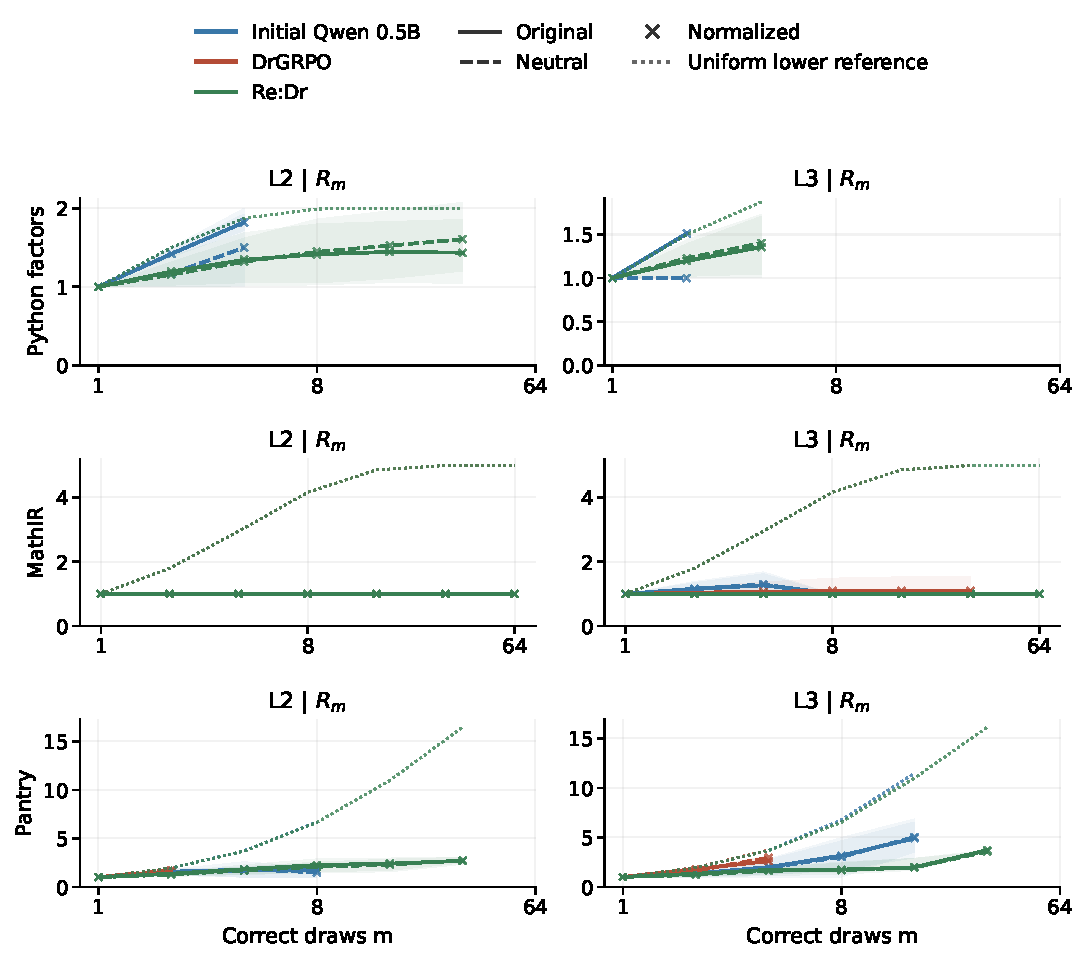
\includegraphics[width=\linewidth,height=0.66\textheight,keepaspectratio]{figures/modebench_discovery_correct_budget_local.pdf}

\caption{\textbf{\texttt{MathIR} correct solutions remain concentrated after training.} Qwen2.5-0.5B-Instruct checkpoints; rows show \texttt{Python}, \texttt{MathIR}, and \texttt{PantryPlan}, and columns Levels~2 and~3. Curves show $R_m$, the expected number of distinct verified modes in $m$ correct draws, on prompts with at least $m$ correct outputs under both wordings. Eligibility varies with $m$, method, and grading; gaps mark undefined means. Dotted lines give uniform lower references on prompts eligible under strict grading in both wordings, with the same prompt and checkpoint weighting as the strict curves. Colours identify methods; solid/dashed lines denote original/neutral wording. Lines use strict verification, crosses formatting normalization, and shading pointwise 95\% bootstrap intervals. Means weight checkpoints equally: five training seeds in \texttt{Python} and \texttt{MathIR}, two in \texttt{PantryPlan}, and one initial checkpoint. Five-seed intervals resample seeds and paired problems; \texttt{PantryPlan} and initial intervals condition on the observed checkpoints for each method.}

\label{fig:discovery-correct-budget-local}

\end{figure}


\subsection{Hosted-model discovery: wording, formatting, and additional draws}
\label{app:hosted-discovery-complete}

The hosted evaluation contains 36,864 responses from GPT-5.4, GPT-5.6 Sol,
and Grok 4.3. Each deployment receives sixteen problems from each of
\texttt{Python}, \texttt{MathIR}, and \texttt{PantryPlan} at Levels~2 and~3,
with two wordings and 64 draws per wording. All three deployments use
medium reasoning effort and an 8,192-token output cap. These settings
differ from the reasoning-disabled main-table evaluation. The \texttt{Python}
comparisons use the same mathematical problems under both wordings.
The hosted models receive no task-specific training in this evaluation.

\paragraph{Neutral wording broadens the GPT models' correct \texttt{MathIR} solutions.}
Both GPT deployments yield at most one verified mode per Level-2 problem
in 64 original-wording draws. Among problems with
at least eight correct responses under both wordings, neutral wording
increases mean breadth at eight correct draws by $.794$ ($[.623,.990]$)
for GPT-5.4 and $.872$ ($[.606,1.123]$) for GPT-5.6 Sol.
The Level-3 effects are $.204$ ($[.106,.320]$) and $.860$
($[.563,1.141]$). These comparisons include fourteen and fifteen jointly
eligible problems at Level~2, respectively, and sixteen for each GPT
deployment at Level~3. Grok 4.3's corresponding intervals include zero at
both levels.

The pointwise intervals resample the sixteen paired problems
within each domain and level, conditioning on the deployment. They do not
include variation across model training seeds. These breadth contrasts
describe jointly eligible problems without equating the wordings' accuracy.

\paragraph{Additional draws reveal more \texttt{PantryPlan} modes after first success.}
Under neutral wording, GPT-5.4 gains $2.583$ and $3.219$ verified modes
between eight and 64 draws at Levels~2 and~3; Grok 4.3 gains $3.377$ and
$4.466$. Grok 4.3's empirical pass probability is already $1.0$ at eight draws
at both levels, so these gains consist entirely of additional modes.
At Level~3 its distinct count rises from $3.972$ to $8.438$.
On jointly eligible problems at eight correct draws, neutral minus
original breadth is $1.781$ ($[1.226,2.338]$) for Grok 4.3 and $.934$
($[.670,1.184]$) for GPT-5.4; GPT-5.6 Sol's Level-3 contrast is
inconclusive. These counts measure finite-sample discovery rather than
exhaustive solution coverage.

\paragraph{Formatting limits GPT-5.6 Sol's strict \texttt{Python} scores.}
GPT-5.6 Sol's original-wording strict pass probability is approximately
$.1875$ at Level~2 and $.0625$ at Level~3 from eight through 64 draws.
Formatting normalization gives $P_{64}=1.0$ under both wordings at both
levels, with all four $P_8$ values above $.989$. The low strict scores
therefore include failures to express valid solutions in the required
format.

After normalization, the neutral-minus-original difference in
discovery gains from eight to 64 draws is $.681$ ($[.351,1.066]$) at Level~2 and $.370$
($[.112,.674]$) at Level~3. Normalization changes response formatting
before applying the same verifier and canonical-key extraction rules.


% Generated by ops/build_paper_gpt56_all_levels32_discovery.py; do not edit.
\subsection{All five domains and all three levels at 512 draws}
\label{app:gpt56-all-levels-discovery}

We evaluate GPT-5.6 Sol on thirty-two problems from each of five domains
at Levels~1, 2, and~3, using the original prompt wording. Problems are
selected independently of model outputs.
Each problem receives 512 responses: 480 problems and 245,760
responses in total. Requests use medium reasoning, an 8,192-token output
limit, and unspecified temperature and top-$p$, with model snapshot
\texttt{gpt-5.6-sol-2026-07-09}. Invalid, refused, and truncated answers remain in the sampling denominator.

Figure~\ref{fig:gpt56-sampling-budget} uses formatting-normalized grading;
Table~\ref{tab:gpt56-all-levels-endpoints} also gives strict-verifier results
on the same response pools. In draw-index order, the first 64 responses
solve 474 of 480 problems after normalization and 418 under strict grading.
At 512 responses, these counts are 477 and 436, respectively.

For a pool of $N=512$ responses, with $c$ correct responses and verified-mode counts $n_j$,
success probability and expected distinct modes in a uniformly sampled $k$-subset are
\[
 P_N(k)=1-\frac{\binom{N-c}{k}}{\binom Nk},\qquad
 D_N(k)=\sum_j\left[1-\frac{\binom{N-n_j}{k}}{\binom Nk}\right],
\]
respectively. We average all thirty-two problems equally within each
domain and level, including problems with no correct response.
Every curve uses the complete 512-response pools at budgets
$k\in\{1,2,4,8,16,32,64,128,256,512\}$. The rarefied estimate at $k=64$
need not equal the result from the first 64 responses in draw-index order.
The gain from the final budget doubling is $D_{512}(512)-D_{512}(256)$.
Pointwise 95\% intervals use 20,000 whole-problem bootstrap replicates
within domain and level; the same resampled problems
form both sides of each contrast. Intervals do not provide simultaneous
coverage across budgets, domains, or levels.

\begin{table}[!htbp]
  \centering
  \footnotesize
  \setlength{\tabcolsep}{4pt}
  \resizebox{\linewidth}{!}{%
  \begin{tabular}{llrrrrr}
    \toprule
    & & & \multicolumn{2}{c}{$D/P$ at 512} & \multicolumn{2}{c}{$\Delta D$, 256 to 512 [95\% CI]} \\
    \cmidrule(lr){4-5}\cmidrule(l){6-7}
    Domain & Level & Known support (range) & Normalized & Strict & Normalized & Strict \\
    \midrule
    \texttt{Graph} & 1 & $6.97$ (4--12) & 2.531/100.0 & 2.531/100.0 & 0.222 [0.142, 0.305] & 0.222 [0.142, 0.305] \\
    \texttt{Graph} & 2 & $6.03$ (4--12) & 2.625/100.0 & 2.625/100.0 & 0.268 [0.170, 0.373] & 0.268 [0.170, 0.373] \\
    \texttt{Graph} & 3 & $6.66$ (4--12) & 1.719/100.0 & 1.719/100.0 & 0.137 [0.059, 0.228] & 0.137 [0.059, 0.228] \\
    \addlinespace[2pt]
    \texttt{Countdown} & 1 & $\geq 4.53$ (2--6) & 3.469/100.0 & 3.375/100.0 & 0.148 [0.070, 0.243] & 0.164 [0.083, 0.259] \\
    \texttt{Countdown} & 2 & $\geq 4.40$ (3--7) & 3.156/100.0 & 3.094/100.0 & 0.218 [0.123, 0.320] & 0.235 [0.136, 0.344] \\
    \texttt{Countdown} & 3 & $\geq 4.25$ (2--8) & 2.812/100.0 & 2.562/100.0 & 0.181 [0.090, 0.289] & 0.191 [0.097, 0.297] \\
    \addlinespace[2pt]
    \texttt{Python} & 1 & $\geq 2.00$ (2) & 3.750/100.0 & 2.875/100.0 & 0.592 [0.438, 0.750] & 0.492 [0.334, 0.656] \\
    \texttt{Python} & 2 & $\geq 2.00$ (2) & 1.438/100.0 & 0.562/43.8 & 0.073 [0.020, 0.135] & 0.148 [0.078, 0.227] \\
    \texttt{Python} & 3 & $\geq 2.00$ (2) & 1.344/100.0 & 0.281/28.1 & 0.013 [0.000, 0.032] & 0.086 [0.031, 0.156] \\
    \addlinespace[2pt]
    \texttt{MathIR} & 1 & $\geq 5.00$ (5) & 1.906/93.8 & 1.906/93.8 & 0.071 [0.012, 0.153] & 0.071 [0.012, 0.153] \\
    \texttt{MathIR} & 2 & $\geq 5.00$ (5) & 1.000/100.0 & 1.000/100.0 & 0.002 [0.000, 0.006] & 0.002 [0.000, 0.006] \\
    \texttt{MathIR} & 3 & $\geq 5.00$ (5) & 0.969/96.9 & 0.969/96.9 & 0.000 [0.000, 0.000] & 0.000 [0.000, 0.000] \\
    \addlinespace[2pt]
    \texttt{PantryPlan} & 1 & $\geq 16.90$ (8--39) & 6.906/100.0 & 6.906/100.0 & 0.622 [0.458, 0.799] & 0.622 [0.458, 0.799] \\
    \texttt{PantryPlan} & 2 & $\geq 16.50$ (8--39) & 4.875/100.0 & 4.625/100.0 & 0.702 [0.476, 0.951] & 0.702 [0.472, 0.962] \\
    \texttt{PantryPlan} & 3 & $\geq 16.87$ (8--40) & 5.562/100.0 & 5.250/100.0 & 0.719 [0.527, 0.914] & 0.678 [0.489, 0.875] \\
    \bottomrule
  \end{tabular}
  }
  \caption{\textbf{Late mode discovery is largest in \texttt{PantryPlan} and Level-1 \texttt{Python}.}
  GPT-5.6 Sol with original wording and 512 responses for each of thirty-two
  problems per domain and level. $D/P$ gives mean distinct verified modes
  and the percentage of problems solved at least once.
  Support gives the mean and range within each domain and level: exact for \texttt{Graph} and a certified
  lower bound elsewhere. Strict and normalized grading use identical pools.
  The paired contrast $\Delta D=D_{512}(512)-D_{512}(256)$ measures the gain
  in expected distinct modes between random subsets of the complete pool, rather than between successive draws.
  Brackets give pointwise 95\% whole-problem bootstrap intervals.}
  \label{tab:gpt56-all-levels-endpoints}
\end{table}

The \texttt{Graph} support count includes every assignment compatible with the fixed colors.
\texttt{Countdown} references enumerate binary expression trees; the validator
also accepts unary negation and retains it in canonical keys, so these
counts are lower bounds. The \texttt{Python}, \texttt{MathIR}, and \texttt{PantryPlan} references
are also certified lower bounds. Exceeding a lower bound does not imply
that all available modes have been discovered.

Figure~\ref{fig:gpt56-sampling-budget} divides the mean distinct-mode count
by the mean enumerated mode count for the same thirty-two problems.
This ratio of means differs from the mean fraction of modes recovered per
problem; the denominator is held fixed when scaling interval endpoints.
The independently certified references in Table~\ref{tab:gpt56-all-levels-endpoints}
can be smaller than these enumerated counts. In \texttt{Python}, the table certifies
at least two modes per problem, while the mean enumerated counts used
in the figure are 222, 335.75, and 354.75 at Levels~1, 2, and~3.

These curves describe random subsets of the observed response pools.
Using them to predict discovery from new responses at each budget also
requires stable sampling behavior across requests; a common model snapshot
and decoding settings do not ensure this. Small or zero gains at the
largest budgets do not rule out rare unseen modes.


\subsection{Discovery at larger sampling budgets}
\label{app:sampling-budget-effects}

The 64-draw comparison in App.~\ref{app:sampling-budget-ablation} uses
36,864 responses from hosted models and 110,592 from Qwen checkpoints,
147,456 in total. Each of the six hosted model--wording combinations
contributes 6,144 responses. The Qwen evaluation includes 25 checkpoints:
each trained checkpoint is evaluated in its training domain at Levels~2
and~3, and the initial checkpoint covers all six domain--level combinations.
Every response remains in its sampling denominator. Formatting normalization
adds no verified Qwen responses, so both grading rules yield identical
estimates for these checkpoints. The sixteen problems per domain and level
differ from the thirty-two used in the 512-draw study
(App.~\ref{app:gpt56-all-levels-discovery}).

\paragraph{Prompt weighting changes the diversity summary.}
Tables~\ref{tab:discovery-breadth-frontier} and~\ref{tab:discovery-breadth-local}
compare two summaries of the 64-response pools. Within each checkpoint or
deployment, collision $C$ pools correct pairs across prompts, weighting each
prompt in proportion to $\binom{c}{2}$. Promptwise \pmd{} gives equal weight
to each prompt with at least two verified responses. Trained-checkpoint
scores then receive equal weight across seeds. Across 70 defined
combinations of model, domain, level, and wording, the median absolute
difference between promptwise \pmd{} and $1-C$ is $.003$, but nineteen
differ by at least $.05$.

For the initial checkpoint under original wording,
Level-2 \texttt{PantryPlan} has $1-C=.151$ and promptwise \pmd{} of $.587$;
Level~3 has $.625$ and $.307$, respectively. Both estimates use seven of
sixteen problems. The direction of the difference depends on which prompts
supply the most correct pairs and therefore receive the largest weights.

Neither weighting holds overall accuracy or the eligible population fixed.
For the initial checkpoint, Level-3 \texttt{Python} has sixteen eligible
problems under original wording and one under neutral wording. Each wording's
absolute estimate uses its own eligible prompts; paired differences use
only jointly eligible prompts. Equal prompt weights therefore describe
conditional diversity within these selected populations
(App.~\ref{app:metric-sampling}).

\paragraph{\texttt{MathIR}: concentration largely persists through 64 draws.}
At Level~2, both trained methods have $B_k=0$ at every measured budget under
both wordings. Re:Dr has $P_8=.9774$ and $P_{64}=.9875$ under original
wording, compared with $.9767$ and $.9875$ under neutral wording. Its $D_k$
equals $P_k$ throughout, so the small increase comes entirely from first
successes. At a budget of eight correct draws, both wordings have $R_8=1$
on the same 76 eligible checkpoint--problem pairs, compared with the
uniform lower reference $5[1-(4/5)^8]=4.1611$ from certified support.
These pairs reuse the same 16 problems across five checkpoints.

At Level~3, both trained methods under neutral wording and Re:Dr under
original wording also yield at most one correct key per checkpoint and
problem. Dr.GRPO under original wording has one exception: one checkpoint--problem
pair contains two keys with counts 28 and 9. Averaging over seeds and problems
gives $B_{64}=.0125$ and $B_{64}-B_8=.0035$. The corresponding equal-seed
correct-pair collision is $.9803$; the other trained \texttt{MathIR}
conditions have collision $1.0$, against the uniform upper reference $.2$.
The larger budget thus reveals a rare additional mode, precluding an exact
single-mode description of every trained condition.

\paragraph{\texttt{Python}: prompt dependence and additional discovery coexist.}
Under original wording, Dr.GRPO has $P_k=D_k=.8125$ at Level~2 and $1.0$
at Level~3 throughout the range from eight to 64 draws. Under neutral wording,
it has zero correct responses out of 5,120 at Level~2 and three out of
5,120 at Level~3. Each success is the only correct response for its
checkpoint--problem pair. The Level~3 mean is therefore
$P_{64}=D_{64}=.0375$, while correct-pair collision remains undefined.

For Re:Dr under original wording, pass probability is unchanged from eight
to 64 draws, but $D_k$ increases by $.0582$ at Level~2 and $.1529$ at
Level~3. Under neutral wording, $P_k$ rises from $.5186$ to $.7500$ and
from $.5109$ to $.7500$, respectively; $D_k$ rises from $.6618$ to $1.1250$
and from $.6561$ to $1.1875$. These final mode counts remain below the
original-wording values of $1.2750$ and $1.5750$. The corresponding gains
in modes beyond the first success are $.2318$ [$.0574,.4565$] and $.2923$
[$.0659,.5445$], with intervals that resample seeds and paired problems.
Larger budgets therefore recover both first successes and additional
verified alternatives for Re:Dr under neutral wording. These unconditional
gains alone do not identify a change in the conditional distribution of
correct solutions.

\paragraph{\texttt{PantryPlan}: eight draws understate observed discovery.}
Across trained checkpoints at both levels and under both wordings,
$D_{64}-D_8$ ranges from $.4151$ to $1.0247$, with gains in modes beyond
the first success ranging from $.2739$ to $.7664$. The initial checkpoint
also gains $.8565$--$1.0778$ modes. For the two observed training seeds,
the Level~3 method ordering changes with the sampling budget. Under original
wording, Dr.GRPO/Re:Dr have $D_8=.2075/.3381$ but
$D_{64}=1.1563/.9063$; neutral wording gives $.2253/.3515$ at eight draws
and $1.2500/.8125$ at 64. These rankings describe the observed checkpoints
and do not establish a population-level method advantage.

\texttt{PantryPlan} has only two training seeds. Comparisons at larger
correct-draw budgets $m$ often have few or no jointly eligible problems.
They condition on observed success, and the equal-seed mean is undefined
when either seed has no eligible problem.

Several trained conditions remain concentrated at 64 draws, while others
continue to yield additional solution modes. A flat curve over a finite
response pool still leaves open the possibility of rare unseen modes.
Here the $k=8$ points average subsets of sixteen 64-response pools per
domain and level; App.~\ref{app:prompt-hint-ablation} uses a separate
eight-draw evaluation on thirty-two problems per domain and level.
The checkpoints are trained at Level~2, so Level~3 results measure transfer;
hosted results describe fixed deployments.


% Concise theory for both papers; full derivations are preserved in
% paper/audits/streamlining_20260911/full_theory.tex.

% Generated by ops/build_paper_inference_followups.py; do not edit numbers.
\section{Inference: Adaptation, Model Mixtures, and Coarser Keys}
\label{app:inference-followups}
We evaluate adaptation to changed requirements, complementarity between
models, and sensitivity to the definition of a solution mode. Model weights
remain fixed during inference. Pointwise 95\% percentile intervals use 20,000
paired whole-problem bootstrap replicates. Resampling preserves all
perturbations, model conditions, and training seeds for each problem;
hosted comparisons resample within each domain and level. These intervals
condition on the observed response pools and training seeds, so they do not
estimate variability across new response pools or training seeds. The 21
model-pair comparisons are dependent, and intervals are unadjusted for
multiple comparisons.

\subsection{\texttt{PantryPlan} portfolios under changed requirements}
\label{app:pantry-adaptation}
We evaluate the initial Qwen2.5-0.5B checkpoint and Level-2 Dr.GRPO and
Re:Dr checkpoints from two matched training seeds on 32 held-out problems.
We derive 192 single-ingredient outages from the task specifications,
independently of generated answers. Exhaustive search over the original
quantity grid finds valid plans for 181 revised tasks. These plans establish
feasibility and are withheld from the model. Five feasible additional dietary
restrictions are reported separately, as they cover only five source problems.

Each portfolio contains eight plans, which we test unchanged against the
revised requirements. If none remains valid, we allow up to eight sequential
recovery calls and stop at the first valid plan. Unresolved portfolios use
all eight calls. Each recovery prompt contains the revised task, initial
portfolio, previous recovery outputs, and deterministic verifier feedback.
Cumulative success includes portfolios that require no recovery. We average
over perturbations within each source problem, then weight problems equally.

The three sampling strategies use the same checkpoints, verifier, and
192-token response cap. Ordinary sampling uses temperature 1.0. Temperature
tuning selects from $\{0.7,1.0,1.3\}$ based on outage survival on 16 separate
development problems (384 responses per checkpoint). Diversity prompting
makes eight sequential calls, requesting a plan with a new ingredient support
and retaining the complete output history, including failures. All strategies
use the same number of initial responses, but their context lengths and total
token costs differ.

\begin{figure}[!htbp]
\centering
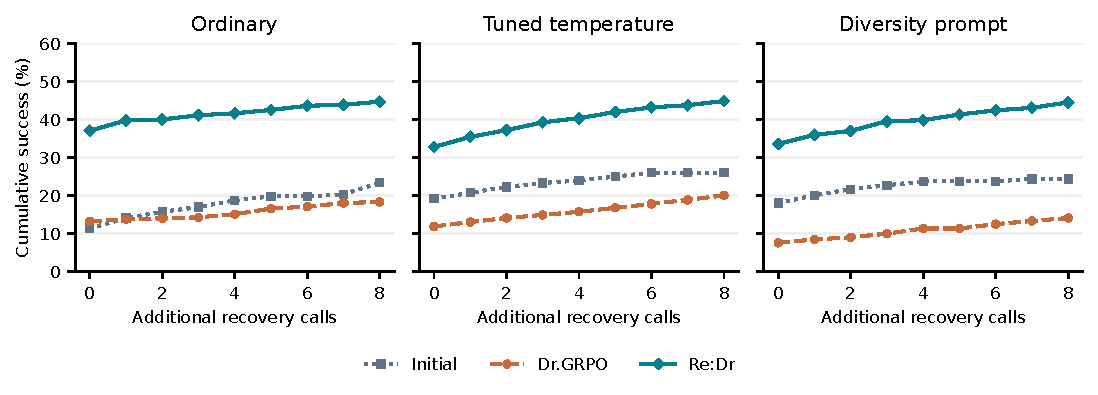
\includegraphics[width=\linewidth]{figures/pantry_adaptation_recovery_20260912.pdf}
\caption{\textbf{Re:Dr improves portfolio survival and success within eight
recovery calls.} Panels compare ordinary sampling, tuned temperature, and
diversity prompting on the same 181 feasible ingredient outages from 32
\texttt{PantryPlan} problems. The horizontal axis is the additional recovery-call budget;
the vertical axis includes success without recovery at zero calls. Curves
average outages within problems, then problems equally. Solid diamonds show
Re:Dr, dashed circles Dr.GRPO, and dotted squares the initial checkpoint;
trained curves average two matched seeds. Pointwise 95\% intervals for
paired differences appear in Table~\ref{tab:pantry-adaptation-contrasts}.}
\label{fig:pantry-adaptation-recovery}
\end{figure}

\begin{table}[!htbp]
\centering
\caption{\textbf{Re:Dr portfolios adapt better to ingredient outages across all three sampling strategies.} Eight initial plans face 181 feasible outages from 32 problems or five additional dietary restrictions from five problems. Survival is success without recovery; By 8 includes success within eight recovery calls (both percentages). Calls count unresolved cases as eight. Token totals count the initial portfolio once per revised task. Entries average perturbations within problems, then problems equally; dietary estimates use only five problems. Labels (a) and (b) denote the two matched training replicates.}
\label{tab:pantry-adaptation}
\scriptsize
\setlength{\tabcolsep}{3pt}
\begin{tabular}{lllrrrrr}
\toprule
Change & Checkpoint & Strategy & Survival & By 8 & Calls & Input tokens & Output tokens \\
\midrule
Outages & Initial & Ordinary & 11.35 & 23.44 & 6.63 & 11301.75 & 376.49 \\
 & Initial & Tuned temperature & 19.17 & 26.04 & 6.13 & 10864.88 & 370.17 \\
 & Initial & Diversity prompt & 18.02 & 24.38 & 6.22 & 11794.81 & 352.87 \\
 & Dr.GRPO (a) & Ordinary & 9.79 & 14.01 & 7.09 & 12439.22 & 823.70 \\
 & Dr.GRPO (a) & Tuned temperature & 13.44 & 16.77 & 6.79 & 12017.57 & 775.44 \\
 & Dr.GRPO (a) & Diversity prompt & 5.21 & 8.39 & 7.44 & 14103.23 & 848.09 \\
 & Dr.GRPO (b) & Ordinary & 16.67 & 22.60 & 6.47 & 11265.39 & 637.59 \\
 & Dr.GRPO (b) & Tuned temperature & 10.31 & 23.39 & 6.75 & 11531.40 & 644.94 \\
 & Dr.GRPO (b) & Diversity prompt & 9.90 & 19.79 & 6.90 & 13124.10 & 731.00 \\
 & Re:Dr (a) & Ordinary & 39.38 & 47.97 & 4.47 & 9078.92 & 297.98 \\
 & Re:Dr (a) & Tuned temperature & 28.23 & 40.94 & 5.19 & 9718.01 & 310.50 \\
 & Re:Dr (a) & Diversity prompt & 36.93 & 47.19 & 4.68 & 10465.22 & 344.02 \\
 & Re:Dr (b) & Ordinary & 34.74 & 41.51 & 4.94 & 9547.16 & 308.52 \\
 & Re:Dr (b) & Tuned temperature & 37.34 & 48.85 & 4.53 & 9148.77 & 300.05 \\
 & Re:Dr (b) & Diversity prompt & 30.26 & 41.93 & 5.06 & 10584.02 & 313.50 \\
\midrule
Dietary & Initial & Ordinary & 0.00 & 20.00 & 6.80 & 11392.80 & 371.20 \\
 & Initial & Tuned temperature & 20.00 & 40.00 & 6.40 & 11175.20 & 387.20 \\
 & Initial & Diversity prompt & 0.00 & 0.00 & 8.00 & 13630.20 & 405.00 \\
 & Dr.GRPO (a) & Ordinary & 0.00 & 0.00 & 8.00 & 13310.20 & 849.20 \\
 & Dr.GRPO (a) & Tuned temperature & 0.00 & 0.00 & 8.00 & 13394.60 & 856.00 \\
 & Dr.GRPO (a) & Diversity prompt & 0.00 & 0.00 & 8.00 & 15045.40 & 939.60 \\
 & Dr.GRPO (b) & Ordinary & 0.00 & 20.00 & 7.40 & 12063.00 & 650.40 \\
 & Dr.GRPO (b) & Tuned temperature & 0.00 & 0.00 & 8.00 & 12544.20 & 615.40 \\
 & Dr.GRPO (b) & Diversity prompt & 0.00 & 0.00 & 8.00 & 14132.40 & 725.60 \\
 & Re:Dr (a) & Ordinary & 20.00 & 60.00 & 5.20 & 9732.60 & 326.00 \\
 & Re:Dr (a) & Tuned temperature & 40.00 & 40.00 & 4.80 & 9402.80 & 307.60 \\
 & Re:Dr (a) & Diversity prompt & 40.00 & 40.00 & 4.80 & 10693.60 & 355.60 \\
 & Re:Dr (b) & Ordinary & 40.00 & 80.00 & 3.20 & 7853.20 & 271.20 \\
 & Re:Dr (b) & Tuned temperature & 40.00 & 80.00 & 3.60 & 8127.80 & 265.20 \\
 & Re:Dr (b) & Diversity prompt & 20.00 & 40.00 & 5.00 & 10738.20 & 341.00 \\
\bottomrule
\end{tabular}
\end{table}


\begin{table}[!htbp]
\centering
\caption{\textbf{Re:Dr raises outage survival and reduces recovery calls.} Entries are Re:Dr minus Dr.GRPO, averaged over two matched seeds on 32 paired problems. Survival and success by eight calls are percentage-point differences; calls include unresolved cases. Brackets are pointwise 95\% paired problem-bootstrap intervals, conditional on the observed training seeds.}
\label{tab:pantry-adaptation-contrasts}
\scriptsize
\setlength{\tabcolsep}{3pt}
\begin{tabular}{lrrr}
\toprule
Strategy & $\Delta$ survival & $\Delta$ by 8 calls & $\Delta$ calls \\
\midrule
Ordinary & $23.83$ $[12.16, 35.89]$ & $26.43$ $[14.69, 38.18]$ & $-2.08$ $[-3.03, -1.14]$ \\
Tuned temperature & $20.91$ $[9.19, 32.89]$ & $24.82$ $[14.04, 35.52]$ & $-1.91$ $[-2.78, -1.05]$ \\
Diversity prompt & $26.04$ $[16.93, 35.65]$ & $30.47$ $[21.51, 39.27]$ & $-2.30$ $[-3.04, -1.57]$ \\
\bottomrule
\end{tabular}
\end{table}

With ordinary sampling, Re:Dr improves survival over Dr.GRPO by 23.83 percentage points
$[12.16,35.89]$, reduces the mean number of recovery calls, capped at eight, by 2.08
$[1.14,3.03]$, and improves success within eight recovery calls by 26.43 points
$[14.69,38.18]$. Mean input and output token totals fall by 2,539.27
$[1,618.01,3,468.86]$ and 427.40 $[386.83,466.30]$, respectively.
The initial portfolios also contain 1.234 more correct responses out of
eight $[.578,1.984]$. Restricting each paired-seed comparison to portfolios
with equal observed correct counts leaves a 1.05-percentage-point survival
gain $[0.00,3.53]$. We first average eligible seed comparisons within each
problem, then average the 19 problems with at least one eligible comparison.
This restriction changes both the problem and seed composition, and equal
observed counts do not establish equal underlying accuracy. The adaptation
gains therefore do not isolate diversity as their causal mechanism.

Per-perturbation token totals represent deploying one portfolio and recovering
from one change in requirements. Input counts include reused prefixes and
do not measure the compute saved by prefix caching. Table~\ref{tab:pantry-collection-cost}
counts each response once across temperature selection, initial portfolios
from tuned-temperature sampling and diversity prompting, and recovery under
all three strategies. It excludes ordinary initial-portfolio generation.
Neither inference cost summary includes training costs.

\begin{table}[!htbp]
\centering
\caption{\textbf{Inference costs include temperature selection and recovery.} Each checkpoint selects $T$ from 384 responses on 16 development problems. Inference totals include this calibration, initial portfolios for tuned-temperature and diversity prompting, and recovery under all three strategies on 32 evaluation problems. Ordinary initial-portfolio generation is excluded. Each response is counted once, including reused input prefixes. Seconds report generation time, excluding training, without hardware normalization. Labels (a) and (b) denote matched training replicates.}
\label{tab:pantry-collection-cost}
\scriptsize
\setlength{\tabcolsep}{3pt}
\begin{tabular}{llrrrrr}
\toprule
Checkpoint & Scope & $T$ & Responses & Input tokens & Output tokens & Seconds \\
\midrule
Dr.GRPO (a) & Calibration & 1.3 & 384 & 229392 & 19871 & 136.3 \\
Dr.GRPO (a) & Inference total & 1.3 & 4874 & 4870884 & 272484 & 3302.0 \\
Dr.GRPO (b) & Calibration & 1.3 & 384 & 229392 & 15544 & 126.5 \\
Dr.GRPO (b) & Inference total & 1.3 & 4634 & 4365524 & 220458 & 2792.9 \\
Re:Dr (a) & Calibration & 0.7 & 384 & 229392 & 8552 & 111.1 \\
Re:Dr (a) & Inference total & 0.7 & 3559 & 3160284 & 92227 & 1527.7 \\
Re:Dr (b) & Calibration & 1.0 & 384 & 229392 & 8585 & 112.5 \\
Re:Dr (b) & Inference total & 1.0 & 3592 & 3169337 & 88300 & 1510.2 \\
Initial & Calibration & 1.3 & 384 & 229392 & 9521 & 123.5 \\
Initial & Inference total & 1.3 & 4416 & 4035069 & 116619 & 1957.4 \\
\bottomrule
\end{tabular}
\end{table}


\subsection{Complementarity across hosted models}
\label{app:cross-model-overlap}
Seven hosted models each produce eight responses to the same 1,920 prompts
(five domains, three levels, and 128 prompts per domain and level), totaling
107,520 responses. We use strict grading and the original Opus 5 \texttt{Python}
interface; the formatting-normalized hosted comparison uses a revised
Opus 5 interface. For each of the 21 model pairs, a mixed portfolio draws four
responses without replacement from each model's eight-response pool. We
compute its expected distinct-mode count exactly over all $\binom{8}{4}^2=4{,}900$
subset pairs, then compare with each constituent's complete eight-response
portfolio and their average. These are expectations within the finite
response pools, conditional on the outputs generated.

Every mixture increases the expected number of distinct solution modes
relative to its average constituent by $.115$--$.266$. Ten pairs improve
on both constituents in point estimates; nine have pointwise intervals
entirely above zero against both. On
prompts with at least four correct responses from each model, we also compare
a mixture of two correct draws per model with four correct draws from either
constituent. All pairwise gains over the average constituent remain positive
($.073$--$.177$ modes). Fixing the number of correct draws conditions on a
different eligible subset for each pair. It does not equate accuracy or the
number of attempts required to obtain those correct responses.

\begin{table}[!htbp]
\centering
\caption{\textbf{Every model pair increases expected distinct modes over its average constituent.} A 4+4 mixture samples without replacement from the two eight-response pools; A and B name the constituents in order. Panel A compares with their average: fine and coarse keys use all 1,920 prompts, while the four-correct-draw comparison uses $n$ prompts with at least four correct responses per model (2+2 mixed versus four per constituent). Panel B compares fine-key distinct modes with each constituent and pass@8 with their average. Entries are distinct-mode differences except pass@8, in percentage points. Brackets are pointwise 95\% paired problem-bootstrap intervals, stratified by domain and level; comparisons share models and prompts.}
\label{tab:cross-model-mixtures}
\scriptsize
\setlength{\tabcolsep}{3pt}
\textbf{A}\par\smallskip
\resizebox{\linewidth}{!}{%
\begin{tabular}{lrrrr}
\toprule
Pair & Fine & Coarse & Four correct draws & $n$ \\
\midrule
DeepSeek V4 Pro + Kimi K3 & $0.148$ $[0.136, 0.160]$ & $0.142$ $[0.131, 0.154]$ & $0.107$ $[0.098, 0.115]$ & 1858 \\
DeepSeek V4 Pro + Opus 4.8 & $0.198$ $[0.185, 0.211]$ & $0.183$ $[0.171, 0.197]$ & $0.153$ $[0.142, 0.164]$ & 1847 \\
DeepSeek V4 Pro + Opus 5 & $0.262$ $[0.249, 0.275]$ & $0.252$ $[0.240, 0.265]$ & $0.177$ $[0.165, 0.190]$ & 1510 \\
DeepSeek V4 Pro + GPT-5.4 & $0.133$ $[0.122, 0.143]$ & $0.127$ $[0.116, 0.138]$ & $0.098$ $[0.090, 0.107]$ & 1695 \\
DeepSeek V4 Pro + GPT-5.6 Sol & $0.235$ $[0.223, 0.247]$ & $0.224$ $[0.212, 0.237]$ & $0.154$ $[0.142, 0.166]$ & 1396 \\
DeepSeek V4 Pro + Grok 4.3 & $0.123$ $[0.112, 0.134]$ & $0.117$ $[0.106, 0.127]$ & $0.091$ $[0.083, 0.099]$ & 1859 \\
Kimi K3 + Opus 4.8 & $0.187$ $[0.174, 0.200]$ & $0.172$ $[0.159, 0.185]$ & $0.138$ $[0.127, 0.148]$ & 1885 \\
Kimi K3 + Opus 5 & $0.266$ $[0.253, 0.279]$ & $0.255$ $[0.242, 0.268]$ & $0.162$ $[0.150, 0.175]$ & 1543 \\
Kimi K3 + GPT-5.4 & $0.127$ $[0.115, 0.139]$ & $0.112$ $[0.101, 0.124]$ & $0.083$ $[0.075, 0.092]$ & 1720 \\
Kimi K3 + GPT-5.6 Sol & $0.202$ $[0.190, 0.214]$ & $0.195$ $[0.183, 0.207]$ & $0.093$ $[0.083, 0.104]$ & 1417 \\
Kimi K3 + Grok 4.3 & $0.115$ $[0.104, 0.126]$ & $0.110$ $[0.099, 0.121]$ & $0.073$ $[0.066, 0.080]$ & 1900 \\
Opus 4.8 + Opus 5 & $0.187$ $[0.176, 0.199]$ & $0.182$ $[0.171, 0.193]$ & $0.098$ $[0.087, 0.109]$ & 1534 \\
Opus 4.8 + GPT-5.4 & $0.201$ $[0.186, 0.215]$ & $0.185$ $[0.172, 0.199]$ & $0.156$ $[0.144, 0.168]$ & 1713 \\
Opus 4.8 + GPT-5.6 Sol & $0.247$ $[0.234, 0.261]$ & $0.237$ $[0.223, 0.250]$ & $0.151$ $[0.138, 0.164]$ & 1409 \\
Opus 4.8 + Grok 4.3 & $0.180$ $[0.167, 0.194]$ & $0.171$ $[0.158, 0.184]$ & $0.141$ $[0.130, 0.153]$ & 1894 \\
Opus 5 + GPT-5.4 & $0.228$ $[0.215, 0.241]$ & $0.217$ $[0.204, 0.230]$ & $0.158$ $[0.145, 0.171]$ & 1493 \\
Opus 5 + GPT-5.6 Sol & $0.169$ $[0.157, 0.182]$ & $0.161$ $[0.149, 0.174]$ & $0.143$ $[0.130, 0.156]$ & 1370 \\
Opus 5 + Grok 4.3 & $0.231$ $[0.219, 0.244]$ & $0.225$ $[0.213, 0.237]$ & $0.145$ $[0.133, 0.157]$ & 1547 \\
GPT-5.4 + GPT-5.6 Sol & $0.156$ $[0.145, 0.167]$ & $0.147$ $[0.136, 0.158]$ & $0.094$ $[0.084, 0.104]$ & 1400 \\
GPT-5.4 + Grok 4.3 & $0.130$ $[0.119, 0.142]$ & $0.121$ $[0.111, 0.132]$ & $0.095$ $[0.086, 0.104]$ & 1722 \\
GPT-5.6 Sol + Grok 4.3 & $0.211$ $[0.199, 0.224]$ & $0.204$ $[0.192, 0.216]$ & $0.118$ $[0.107, 0.130]$ & 1418 \\
\bottomrule
\end{tabular}
}
\par\medskip
\textbf{B}\par\smallskip
\resizebox{\linewidth}{!}{%
\begin{tabular}{lrrr}
\toprule
Pair & $\Delta D$ vs A & $\Delta D$ vs B & $\Delta$ pass@8 vs mean \\
\midrule
DeepSeek V4 Pro + Kimi K3 & $0.279$ $[0.254, 0.304]$ & $0.017$ $[-0.008, 0.043]$ & $0.22$ $[0.08, 0.39]$ \\
DeepSeek V4 Pro + Opus 4.8 & $0.089$ $[0.064, 0.114]$ & $0.307$ $[0.282, 0.332]$ & $0.31$ $[0.15, 0.49]$ \\
DeepSeek V4 Pro + Opus 5 & $-0.061$ $[-0.082, -0.039]$ & $0.585$ $[0.560, 0.610]$ & $7.48$ $[7.19, 7.78]$ \\
DeepSeek V4 Pro + GPT-5.4 & $0.097$ $[0.074, 0.121]$ & $0.168$ $[0.145, 0.192]$ & $0.64$ $[0.41, 0.90]$ \\
DeepSeek V4 Pro + GPT-5.6 Sol & $-0.003$ $[-0.025, 0.019]$ & $0.473$ $[0.447, 0.500]$ & $7.16$ $[6.71, 7.62]$ \\
DeepSeek V4 Pro + Grok 4.3 & $0.059$ $[0.037, 0.082]$ & $0.186$ $[0.163, 0.210]$ & $0.34$ $[0.17, 0.52]$ \\
Kimi K3 + Opus 4.8 & $-0.053$ $[-0.080, -0.027]$ & $0.427$ $[0.401, 0.452]$ & $0.19$ $[0.07, 0.32]$ \\
Kimi K3 + Opus 5 & $-0.188$ $[-0.212, -0.165]$ & $0.719$ $[0.692, 0.747]$ & $7.34$ $[7.08, 7.61]$ \\
Kimi K3 + GPT-5.4 & $-0.040$ $[-0.064, -0.015]$ & $0.293$ $[0.267, 0.320]$ & $0.73$ $[0.48, 1.00]$ \\
Kimi K3 + GPT-5.6 Sol & $-0.167$ $[-0.191, -0.144]$ & $0.571$ $[0.543, 0.600]$ & $7.38$ $[6.92, 7.85]$ \\
Kimi K3 + Grok 4.3 & $-0.080$ $[-0.104, -0.056]$ & $0.309$ $[0.284, 0.335]$ & $0.12$ $[0.03, 0.23]$ \\
Opus 4.8 + Opus 5 & $-0.027$ $[-0.045, -0.009]$ & $0.401$ $[0.379, 0.423]$ & $7.42$ $[7.14, 7.71]$ \\
Opus 4.8 + GPT-5.4 & $0.274$ $[0.248, 0.300]$ & $0.127$ $[0.101, 0.153]$ & $0.93$ $[0.65, 1.24]$ \\
Opus 4.8 + GPT-5.6 Sol & $0.118$ $[0.096, 0.141]$ & $0.377$ $[0.350, 0.403]$ & $7.51$ $[7.03, 7.99]$ \\
Opus 4.8 + Grok 4.3 & $0.226$ $[0.202, 0.250]$ & $0.135$ $[0.110, 0.160]$ & $0.11$ $[0.02, 0.23]$ \\
Opus 5 + GPT-5.4 & $0.515$ $[0.489, 0.541]$ & $-0.060$ $[-0.082, -0.037]$ & $6.30$ $[5.90, 6.71]$ \\
Opus 5 + GPT-5.6 Sol & $0.254$ $[0.232, 0.277]$ & $0.084$ $[0.063, 0.106]$ & $2.11$ $[1.66, 2.57]$ \\
Opus 5 + Grok 4.3 & $0.490$ $[0.467, 0.514]$ & $-0.028$ $[-0.048, -0.007]$ & $7.41$ $[7.13, 7.69]$ \\
GPT-5.4 + GPT-5.6 Sol & $-0.046$ $[-0.067, -0.025]$ & $0.359$ $[0.335, 0.383]$ & $5.61$ $[5.15, 6.08]$ \\
GPT-5.4 + Grok 4.3 & $0.102$ $[0.078, 0.127]$ & $0.159$ $[0.135, 0.182]$ & $0.93$ $[0.65, 1.23]$ \\
GPT-5.6 Sol + Grok 4.3 & $0.386$ $[0.360, 0.412]$ & $0.037$ $[0.015, 0.058]$ & $7.55$ $[7.08, 8.04]$ \\
\bottomrule
\end{tabular}
}
\end{table}

Cross-model collision ranges from $.624$ to $.740$, compared with $.704$
to $.819$ for mean within-model collision. Each pair gives equal weight
to prompts with $\geq2$ correct responses from each model. Absence of
observed overlap does not establish disjoint supports. Gains relative to
the average constituent persist with coarser keys and formatting-normalized
grading. Equal response counts do not equate token use, compute, monetary
cost, or reasoning interfaces across providers. These comparisons of finite
response pools do not identify causal training mechanisms.

\subsection{Sensitivity to task-relevant equivalences}
\label{app:coarser-keys}
We merge solution keys according to task-relevant equivalences and recompute
diversity. \texttt{Graph} merges global color renamings that fix every anchored color;
vertex identities remain fixed. \texttt{Python} groups opposite members $d$ and $n/d$ of the
same unordered proper factor pair, retaining input-vector order. \texttt{Countdown}
flattens associative additions and multiplications and sorts their children,
preserving operands, multiplicity, and subtraction/division boundaries.
\texttt{MathIR} retains its simplified state trajectory, and \texttt{PantryPlan} retains
ingredient supports, whose differences can affect survival under outages. The same domain-specific
map applies to each model's correct responses. Correctness is unchanged;
deterministic merging cannot increase the observed distinct-mode count or
reduce correct-pair collision.

Uniform mass over fine keys generally induces unequal mass across coarse
groups. For \texttt{Graph} and \texttt{Python}, exhaustive enumeration determines both the
number of coarse groups and their sizes, allowing separate collision
references for uniform fine-key mass and uniform coarse-group mass.
\texttt{Countdown}'s full verifier support is unknown, so these uniform references
cannot be computed for that domain.

\begin{table}[!htbp]
\centering
\caption{\textbf{Coarser keys reduce observed mode counts and increase collision.} Strict grading uses eight responses per hosted model on 1,920 prompts. $D@8$ averages all prompts; collision averages prompts with at least two correct responses, with eligibility varying by model. Brackets are pointwise 95\% paired problem-bootstrap intervals, stratified by domain and level.}
\label{tab:hosted-coarse-keys}
\scriptsize
\setlength{\tabcolsep}{3pt}
\begin{tabular}{lrrrr}
\toprule
Model & Fine D@8 & Coarse D@8 & Fine collision & Coarse collision \\
\midrule
DeepSeek V4 Pro & $1.826$ $[1.792, 1.859]$ & $1.762$ $[1.729, 1.795]$ & $0.720$ $[0.710, 0.731]$ & $0.739$ $[0.729, 0.750]$ \\
Kimi K3 & $2.087$ $[2.047, 2.129]$ & $1.952$ $[1.913, 1.992]$ & $0.688$ $[0.678, 0.699]$ & $0.723$ $[0.712, 0.733]$ \\
Opus 4.8 & $1.608$ $[1.575, 1.641]$ & $1.556$ $[1.525, 1.588]$ & $0.795$ $[0.785, 0.805]$ & $0.811$ $[0.801, 0.821]$ \\
Opus 5 & $1.180$ $[1.155, 1.206]$ & $1.152$ $[1.128, 1.177]$ & $0.856$ $[0.845, 0.866]$ & $0.867$ $[0.857, 0.877]$ \\
GPT-5.4 & $1.755$ $[1.718, 1.792]$ & $1.679$ $[1.644, 1.715]$ & $0.729$ $[0.717, 0.741]$ & $0.750$ $[0.739, 0.762]$ \\
GPT-5.6 Sol & $1.349$ $[1.317, 1.382]$ & $1.312$ $[1.281, 1.345]$ & $0.778$ $[0.765, 0.790]$ & $0.794$ $[0.782, 0.806]$ \\
Grok 4.3 & $1.698$ $[1.665, 1.732]$ & $1.645$ $[1.613, 1.679]$ & $0.791$ $[0.782, 0.800]$ & $0.807$ $[0.798, 0.816]$ \\
\bottomrule
\end{tabular}
\end{table}


\begin{table}[!htbp]
\centering
\caption{\textbf{\texttt{Python} diversity gains depend on the factor-pair equivalence and prompt wording.} Entries give Re:Dr minus Dr.GRPO in distinct modes from eight strictly graded responses. Level-2 trained Qwen2.5-0.5B checkpoints use 32 paired evaluation problems per level; means weight seeds equally. Brackets are pointwise 95\% paired problem-bootstrap intervals, conditional on those checkpoints. Fine and coarse keys coincide for \texttt{MathIR} and \texttt{PantryPlan}.}
\label{tab:local-coarse-keys}
\scriptsize
\setlength{\tabcolsep}{3pt}
\begin{tabular}{lrllrr}
\toprule
Domain & Level & Wording & Seeds & Fine $\Delta D@8$ & Coarse $\Delta D@8$ \\
\midrule
\texttt{Python} & 2 & original & 5 & $0.431$ $[0.406, 0.456]$ & $0.075$ $[0.025, 0.138]$ \\
\texttt{MathIR} & 2 & original & 5 & $0.463$ $[0.387, 0.531]$ & $0.463$ $[0.387, 0.531]$ \\
\texttt{PantryPlan} & 2 & original & 2 & $0.469$ $[0.203, 0.750]$ & $0.469$ $[0.203, 0.750]$ \\
\texttt{Python} & 3 & original & 5 & $0.419$ $[0.400, 0.444]$ & $0.000$ $[0.000, 0.000]$ \\
\texttt{MathIR} & 3 & original & 5 & $0.119$ $[0.019, 0.225]$ & $0.119$ $[0.019, 0.225]$ \\
\texttt{PantryPlan} & 3 & original & 2 & $0.125$ $[-0.109, 0.375]$ & $0.125$ $[-0.109, 0.375]$ \\
\texttt{Python} & 2 & neutral & 5 & $0.675$ $[0.519, 0.838]$ & $0.556$ $[0.438, 0.675]$ \\
\texttt{MathIR} & 2 & neutral & 5 & $0.469$ $[0.375, 0.562]$ & $0.469$ $[0.375, 0.562]$ \\
\texttt{PantryPlan} & 2 & neutral & 2 & $0.484$ $[0.234, 0.766]$ & $0.484$ $[0.234, 0.766]$ \\
\texttt{Python} & 3 & neutral & 5 & $0.656$ $[0.537, 0.775]$ & $0.500$ $[0.419, 0.575]$ \\
\texttt{MathIR} & 3 & neutral & 5 & $0.119$ $[0.025, 0.213]$ & $0.119$ $[0.025, 0.213]$ \\
\texttt{PantryPlan} & 3 & neutral & 2 & $0.250$ $[-0.031, 0.562]$ & $0.250$ $[-0.031, 0.562]$ \\
\bottomrule
\end{tabular}
\end{table}

With coarser \texttt{Python} keys, the Re:Dr-minus-Dr.GRPO gain in distinct modes
under original wording falls from $.419$ to zero at Level~3 and from
$.431$ to $.075$ at Level~2. Under neutral wording, the gains remain
$.556$ at Level~2 and $.500$ at Level~3. The original-wording effect can
therefore reflect opposite members of the same factor pair. Its interpretation
depends on both prompt wording and the definition of a solution mode;
neither divisor vectors nor factor-pair vectors identify different algorithms.


% Generated by ops/build_paper_portfolio_withdrawals.py; do not edit numbers.
\section{Portfolio Survival under Withdrawn Options}
\label{app:portfolio-withdrawals}
A portfolio survives a withdrawn option if at least one of its solutions
remains valid. We evaluate survival across all five domains in 474 terminal checkpoint evaluations, each
with 128 prompts and four groups of eight responses per prompt. The groups have
overlapping sampling streams (App.~\ref{app:conditional-concentration}). Replay's
largest gains in expected distinct modes at four verified draws occur in
\texttt{Graph}, \texttt{Countdown}, \texttt{Python} and \texttt{PantryPlan}. Across 38 matched
domain--scale--level--objective comparisons,
\pmd{} gains correlate with survival gains at four verified draws
(Pearson $r=.57$).

\paragraph{Task perturbations.} Each task loses one option: a colour at one
vertex (\texttt{Graph}), an arithmetic operation (\texttt{Countdown}), a returned divisor value
(\texttt{Python}), a menu action (\texttt{MathIR}), or an ingredient (\texttt{PantryPlan}; see
App.~\ref{app:pantry-adaptation}). Options are enumerated from the task
specification. The solution-mode enumeration matches the certified counts for
all 1{,}280 prompts. A surviving certified mode establishes feasibility.
When the certified count is only a lower bound on the verifier's full support,
absence of a surviving mode from the enumeration does not establish infeasibility. Of
9{,}864 options, 9{,}118 retain at least one certified mode. Among these,
8{,}308 are binding: they also remove at least one certified mode. We evaluate
both the binding set and the full set with a feasibility certificate.

\paragraph{Survival criterion.} Each portfolio contains the verified
responses among eight draws. It survives when at least one of these solutions
remains valid after the option is removed. \texttt{Graph}, \texttt{Countdown} and \texttt{Python} determine this directly from
the outcome key, including verified keys outside the enumeration. \texttt{Countdown}
contributes 2 such keys, observed 50 times among the
846{,}398 verified draws in this evaluation: the verifier accepts unary negation, which the
expression enumeration omits. For \texttt{MathIR}, re-enumerating the reduced menu tests
whether the same executed state path remains realizable, possibly through a
different action sequence. For \texttt{PantryPlan}, we test the certified plan
associated with each ingredient-support key. All observed \texttt{MathIR} and \texttt{PantryPlan} keys belong to their
respective enumerations.

\paragraph{Survival conditional on correct draws.} Raw survival depends on
both correctness and the distribution of valid modes. At budgets $m=1,2,4$, we
compute the exact expected survival of a uniformly selected $m$-element subset
of a portfolio's verified draws, as in App.~\ref{app:cross-model-overlap}.
Replay--control contrasts use only prompt--group pairs with at least $m$
verified draws under both methods, so eligibility can change with $m$.
Fixing the number of correct draws does not equalize policy accuracy.
A survival difference can also arise because the modes one method favors are
individually more robust to withdrawals, so a gain that grows with $m$ does
not by itself isolate the contribution of diversity. Expected distinct modes
at the same budget therefore serve as a separate measure of portfolio breadth.

\begin{table}[!htbp]
\centering
\caption{\textbf{Binding withdrawals remove certified modes while retaining a feasibility certificate.} Each row covers 128 prompts. Support is the mean certified mode count per prompt; Options counts single withdrawals. Binding counts options that retain at least one certified mode and remove at least one. Kept is the mean retained fraction of certified modes across binding options. Pairs counts binding pairs of withdrawals, and Kept$_2$ gives the corresponding retained fraction.}
\label{tab:withdrawal-inventory}
\scriptsize
\setlength{\tabcolsep}{3pt}
\begin{tabular}{llrrrrrrr}
\toprule
Domain & Level & Prompts & Support & Options & Binding & Kept & Pairs & Kept$_2$ \\
\midrule
\texttt{Graph} & 1 & 128 & 6.3 & 1152 & 818 & 0.57 & 1957 & 0.34 \\
\texttt{Graph} & 2 & 128 & 6.1 & 1536 & 1068 & 0.57 & 3457 & 0.35 \\
\texttt{Countdown} & 1 & 128 & 4.5 & 512 & 147 & 0.48 & 21 & 0.44 \\
\texttt{Countdown} & 2 & 128 & 4.4 & 512 & 185 & 0.49 & 40 & 0.37 \\
\texttt{Python} & 1 & 128 & 229.4 & 1433 & 1433 & 0.68 & 7716 & 0.50 \\
\texttt{Python} & 2 & 128 & 251.7 & 1647 & 1647 & 0.71 & 10381 & 0.55 \\
\texttt{MathIR} & 1 & 128 & 5.0 & 768 & 448 & 0.40 & 384 & 0.23 \\
\texttt{MathIR} & 2 & 128 & 5.0 & 768 & 512 & 0.45 & 512 & 0.25 \\
\texttt{PantryPlan} & 1 & 128 & 18.2 & 768 & 651 & 0.44 & 1231 & 0.18 \\
\texttt{PantryPlan} & 2 & 128 & 18.2 & 768 & 653 & 0.45 & 1228 & 0.19 \\
\bottomrule
\end{tabular}
\end{table}
\begin{table}[!htbp]
\centering
\caption{\textbf{Both replay arms improve four-draw survival in \texttt{Graph}, \texttt{Python} and \texttt{PantryPlan}.} Each replay arm is compared with its fresh-objective control. Survival differences are percentage points; $\Delta D_4$ is the difference in expected distinct modes at four verified draws. Raw uses all eight responses; Budget columns use the indicated number of verified draws. Fixed-correct-draw results pool jointly eligible prompt--group pairs across matched seeds, scales and levels; raw results use all paired groups. All columns use binding options except Budget 4 (all), which includes every option with a feasibility certificate. Brackets are pointwise 95\% intervals from 20{,}000 paired bootstrap replicates. Each resampled cluster is a prompt within one level and scale, with its groups and seeds kept together; copies at other scales are separate clusters. Intervals condition on the observed seeds.}
\label{tab:withdrawal-contrasts}
\scriptsize
\setlength{\tabcolsep}{3pt}
\begin{tabular}{llrrrrrr}
\toprule
Domain & Arm & Raw & Budget 1 & Budget 2 & Budget 4 & Budget 4 (all) & $\Delta D_4$ \\
\midrule
\texttt{Graph} & Re:Dr & $34.78$ & $0.00$ $[0.00, 0.00]$ & $10.51$ $[8.76, 12.31]$ & $19.65$ $[15.61, 23.82]$ & $15.66$ & 1.290 \\
\texttt{Graph} & Re:Max & $18.98$ & $0.00$ $[0.00, 0.00]$ & $6.62$ $[5.23, 7.98]$ & $10.99$ $[8.25, 13.81]$ & $8.31$ & 0.646 \\
\texttt{Countdown} & Re:Dr & $5.32$ & $3.51$ $[1.88, 5.30]$ & $6.52$ $[4.27, 8.94]$ & $9.58$ $[6.81, 12.63]$ & $2.53$ & 0.626 \\
\texttt{Countdown} & Re:Max & $1.95$ & $-2.40$ $[-4.62, -0.21]$ & $-1.25$ $[-3.70, 1.14]$ & $0.10$ $[-2.62, 2.78]$ & $-0.05$ & 0.490 \\
\texttt{Python} & Re:Dr & $38.99$ & $-0.22$ $[-1.25, 0.91]$ & $4.09$ $[3.17, 5.08]$ & $7.67$ $[6.82, 8.58]$ & $7.67$ & 0.317 \\
\texttt{Python} & Re:Max & $22.84$ & $1.53$ $[0.87, 2.24]$ & $3.85$ $[3.04, 4.72]$ & $5.68$ $[4.80, 6.64]$ & $5.68$ & 0.198 \\
\texttt{MathIR} & Re:Dr & $33.61$ & $0.01$ $[0.00, 0.05]$ & $0.12$ $[0.03, 0.23]$ & $0.14$ $[0.00, 0.30]$ & $0.08$ & 0.004 \\
\texttt{MathIR} & Re:Max & $21.64$ & $0.00$ $[-0.04, 0.05]$ & $0.03$ $[-0.03, 0.10]$ & $0.09$ $[-0.01, 0.21]$ & $0.06$ & 0.003 \\
\texttt{PantryPlan} & Re:Dr & $16.55$ & $-1.11$ $[-1.65, -0.54]$ & $4.36$ $[3.82, 4.87]$ & $9.78$ $[8.90, 10.65]$ & $9.20$ & 0.810 \\
\texttt{PantryPlan} & Re:Max & $13.04$ & $-0.64$ $[-1.04, -0.21]$ & $3.12$ $[2.72, 3.53]$ & $6.61$ $[5.83, 7.39]$ & $6.20$ & 0.547 \\
\bottomrule
\end{tabular}
\end{table}
Raw survival improves in 39 of 40 domain--scale--level--objective
comparisons. At four verified draws, the point estimate is positive in
28 of 39 eligible comparisons; these conditional comparisons cover
fewer prompt--group pairs than raw survival. Outside \texttt{MathIR}, Re:Dr adds between
$.3$ and $1.3$ expected distinct modes at four verified draws, and its pooled
survival gains reach 19.6 percentage points. In \texttt{MathIR}, the corresponding
gains are only $.004$ distinct modes and $.14$ survival points, with an interval
of $[.00,.30]$ after rounding. These small positive estimates are consistent
with the small \pmd{} gain in Table~\ref{tab:cross-scale-terminal-effects}.

\texttt{Graph}'s one-draw contrast is zero by construction. Each binding withdrawal
removes one color at one vertex, and each valid coloring is excluded by
exactly one such withdrawal per variable vertex, so every individual mode
survives the same fraction of binding withdrawals. Including nonbinding options shrinks the contrasts,
because those options leave every certified mode intact; for example,
63\% of \texttt{Countdown} Level-1 options with a feasibility certificate are nonbinding.
The Budget 4 (all) and binding columns therefore describe different withdrawal
populations.
\begin{figure}[!htbp]
  \centering
  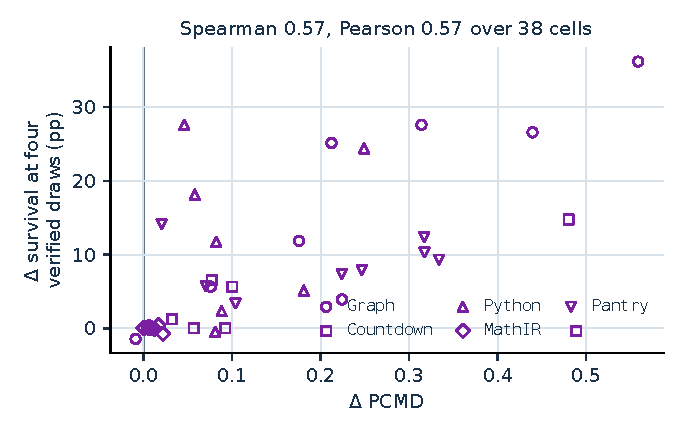
\includegraphics[width=0.62\linewidth]{figures/withdrawal_pmd_agreement.pdf}
  \caption{\textbf{Diversity gains correlate with survival gains after a withdrawal.} Each mark is one replay--fresh-objective contrast in a domain, scale and level. The horizontal axis is the terminal \pmd{} difference; the vertical axis is the percentage-point survival difference at four verified draws, averaged equally over eligible seed-specific contrasts. Survival uses jointly eligible prompt--group pairs within each seed. Marker shape identifies the domain; zero lines mark no change. The 38 comparisons have Pearson and Spearman correlations of $.57$; points show estimates without intervals. The association is descriptive, and the two metrics need not use the same eligible population.}
  \label{fig:withdrawal-pmd-agreement}
\end{figure}

\subsection{Two withdrawals at once}
\label{app:withdrawal-severity}
We next remove two binding options at once. Of the 29{,}213 pairs of binding
single withdrawals, 26{,}927 retain at least one certified mode and enter the
survival comparison. For \texttt{Graph}, \texttt{Countdown}, \texttt{Python} and \texttt{PantryPlan},
a certified mode survives the pair exactly when it survives both individual
withdrawals. \texttt{MathIR} can differ: removing two actions can eliminate every
realization of a state path even when either action alone can be removed.
Re-enumerating the reduced menus shows that no such case occurs here: for all
1{,}344 \texttt{MathIR} pairs, including those that leave no certified mode,
the surviving set equals the intersection of the two single-withdrawal sets.

\begin{table}[!htbp]
\centering
\caption{\textbf{Two withdrawals retain survival gains in \texttt{Graph}, \texttt{Python} and \texttt{PantryPlan}.} Entries are replay--fresh-objective differences in percentage points at two (@2) or four (@4) verified draws. One uses binding single options; Two uses binding pairs with a feasibility certificate. Their eligible prompt populations can differ. Estimates pool jointly eligible groups. Brackets are pointwise 95\% paired prompt-bootstrap intervals with the clustering in Table~\ref{tab:withdrawal-contrasts}.}
\label{tab:withdrawal-severity}
\scriptsize
\setlength{\tabcolsep}{3pt}
\begin{tabular}{llrrrr}
\toprule
Domain & Arm & One @2 & One @4 & Two @2 & Two @4 \\
\midrule
\texttt{Graph} & Re:Dr & $10.51$ & $19.65$ $[15.61, 23.82]$ & $10.02$ & $23.65$ $[19.14, 28.25]$ \\
\texttt{Graph} & Re:Max & $6.62$ & $10.99$ $[8.25, 13.81]$ & $5.93$ & $12.51$ $[9.37, 15.69]$ \\
\texttt{Countdown} & Re:Dr & $6.52$ & $9.58$ $[6.81, 12.63]$ & $3.29$ & $6.11$ $[0.87, 12.22]$ \\
\texttt{Countdown} & Re:Max & $-1.25$ & $0.10$ $[-2.62, 2.78]$ & $-5.53$ & $-4.87$ $[-11.80, 0.76]$ \\
\texttt{Python} & Re:Dr & $4.09$ & $7.67$ $[6.82, 8.58]$ & $5.37$ & $10.10$ $[8.77, 11.55]$ \\
\texttt{Python} & Re:Max & $3.85$ & $5.68$ $[4.80, 6.64]$ & $5.64$ & $8.16$ $[6.79, 9.64]$ \\
\texttt{MathIR} & Re:Dr & $0.12$ & $0.14$ $[0.00, 0.30]$ & $0.18$ & $0.20$ $[0.01, 0.45]$ \\
\texttt{MathIR} & Re:Max & $0.03$ & $0.09$ $[-0.01, 0.21]$ & $0.04$ & $0.12$ $[-0.01, 0.29]$ \\
\texttt{PantryPlan} & Re:Dr & $4.36$ & $9.78$ $[8.90, 10.65]$ & $2.85$ & $7.23$ $[6.51, 7.95]$ \\
\texttt{PantryPlan} & Re:Max & $3.12$ & $6.61$ $[5.83, 7.39]$ & $2.03$ & $4.94$ $[4.35, 5.57]$ \\
\bottomrule
\end{tabular}
\end{table}

Two withdrawals retain less certified support on average
(Table~\ref{tab:withdrawal-inventory}). Re:Dr's pooled survival gain at four
verified draws rises in \texttt{Graph}, \texttt{Python} and \texttt{MathIR}, and falls in \texttt{Countdown} and
\texttt{PantryPlan}. \texttt{Countdown} Level 1 starts with only 4.5 certified modes per prompt;
\texttt{PantryPlan} Level 1 retains only 18\% of its certified modes under a binding pair.
These support differences coincide with the smaller gains but do not
establish their cause. Across domain--scale--level--objective comparisons,
25 of 39 point estimates are positive at four verified draws,
compared with 28 of 39 for single withdrawals.

\subsection{Decoding settings as a substitute}
\label{app:withdrawal-decoding}
Can a better decoding setting give an ordinary policy the same survival?
We evaluate binding Level-1 withdrawals on 128 prompts per domain, using the
separate Qwen2.5-0.5B cohort trained for twelve passes in
App.~\ref{app:decoding-objection}. Its replay variant combines separate mass
and within-buffer balancing terms with novelty and semantic-entropy shaping;
it differs from Re:Dr in both objective and training duration. Five seeds per
arm are evaluated at 11 settings: six temperatures from $.5$ to $2.0$,
three settings with larger groups, and two with top-$p=.95$. Larger groups
increase $K$ from 8 to 32, but use two groups rather than four: total responses
per prompt double from 32 to 64. The reference is $T=1$, top-$p=1$, and four
groups of eight. For each domain, we select the control setting with the
highest four-verified-draw survival on these evaluation prompts, while replay
keeps the reference setting.

\begin{table}[!htbp]
\centering
\caption{\textbf{Replay survival exceeds the selected control setting in all five domains.} Survival at four verified draws is expressed as percentages. Control, Control grid and Replay are equal-seed means on each setting's own eligible groups; the grid column gives the control range and Best its maximizing temperature. $\Delta$ instead pools jointly eligible groups for reference replay minus selected control, so it need not equal the difference of the displayed means. Brackets are pointwise 95\% intervals from 20{,}000 paired prompt-bootstrap replicates, keeping all groups and five seeds of a prompt together. The selected setting stays fixed in the bootstrap; intervals condition on that selection and the seeds.}
\label{tab:withdrawal-decoding}
\scriptsize
\setlength{\tabcolsep}{3pt}
\begin{tabular}{lrrcrr}
\toprule
Domain & Control & Control grid & Best & Replay & $\Delta$ vs best \\
\midrule
\texttt{Graph} & 58.61 & 58.59--58.85 & $T{=}2$ & 95.91 & $36.97$ $[35.53, 38.42]$ \\
\texttt{Countdown} & 15.49 & 12.57--16.16 & $T{=}1.6$ & 40.09 & $28.87$ $[18.98, 38.87]$ \\
\texttt{Python} & 70.54 & 70.36--70.54 & $T{=}0.5$ & 77.56 & $8.33$ $[7.15, 9.69]$ \\
\texttt{MathIR} & 72.23 & 72.18--72.55 & $T{=}2$ & 73.60 & $1.37$ $[0.61, 2.30]$ \\
\texttt{PantryPlan} & 50.65 & 50.02--51.79 & $T{=}2$ & 64.09 & $12.73$ $[10.22, 15.31]$ \\
\bottomrule
\end{tabular}
\end{table}

Control survival spans at most 3.6 percentage points across the grid.
The paired replay gains range from 1.4 to 37.0 points, with all five
pointwise intervals above zero. Every selected control setting changes only the
temperature, keeping eight-response groups and top-$p=1$. The tested decoding
changes therefore do not close the survival gap in this cohort. Because each
control setting is selected on the evaluation prompts, the control's survival
is, if anything, optimistic for new prompts. Finite samples cannot show that
the missing alternative modes have zero probability under the control.

\subsection{Recovery after a withdrawal}
\label{app:withdrawal-recovery}
Recovery is evaluated at the Level-1 Qwen2.5-0.5B terminal Dr.GRPO and Re:Dr
checkpoints from two matched training seeds in each of five domains. Each domain has 32 test and 16 temperature-calibration prompts in a
disjoint split. Prompts without a binding withdrawal that retains a certified
mode are excluded, leaving 28 test and 15 calibration prompts in \texttt{Countdown} and all
prompts elsewhere. Up to four binding options per test prompt give
533 distinct withdrawals, shared by both arms and seeds.

Each initial portfolio contains eight responses. Ordinary sampling uses its
terminal evaluation group at $T=1$. The temperature strategy generates a group
at the temperature in $\{.7,1.0,1.3\}$ maximizing mean survival on the
calibration prompts. The diversity-prompt strategy generates the eight
responses sequentially, with the preceding responses included in each request.
All strategies share the same recovery procedure. If no initial mode survives,
the model generates one response per call at $T=1$, for up to eight calls,
with the revised task, the initial portfolio and previous failed attempts in
context. Recovery stops at the first verified response whose mode survives the
withdrawal.

Survival uses the mode predicates defined above. In \texttt{MathIR}, a retained or newly
generated state path can count as surviving even if realizing it under the
reduced menu requires a different action sequence. \texttt{PantryPlan} responses are
six-bit ingredient-support masks projected onto verified quantities by the
environment (App.~\ref{app:prompt-pantry}); survival is evaluated on the resulting
support key. These outcomes therefore measure whether a mode remains feasible,
not whether the original response text can be reused unchanged.

\begin{table}[!htbp]
\centering
\caption{\textbf{Replay improves ordinary and temperature-tuned recovery in every domain.} Saved is the percentage of withdrawals with a surviving initial mode; By 8 also counts those resolved within eight additional responses. Calls is the mean additional response count, with zero for initial survival and eight for unresolved cases. Each row pools the same withdrawals over two matched seeds. Fresh is Dr.GRPO and Replay is Re:Dr; the three strategies differ only in initial portfolio generation.}
\label{tab:withdrawal-recovery}
\scriptsize
\setlength{\tabcolsep}{3pt}
\begin{tabular}{llrrrrrr}
\toprule
Domain & Strategy & Fresh saved & Fresh by 8 & Fresh calls & Replay saved & Replay by 8 & Replay calls \\
\midrule
\texttt{Graph} & Ordinary & 15.62 & 22.66 & 6.38 & 83.20 & 91.02 & 1.01 \\
\texttt{Graph} & Tuned temperature & 15.62 & 20.31 & 6.55 & 77.34 & 89.06 & 1.36 \\
\texttt{Graph} & Diversity prompt & 29.69 & 30.47 & 5.58 & 62.50 & 74.61 & 2.44 \\
\texttt{Countdown} & Ordinary & 2.70 & 2.70 & 7.78 & 9.46 & 10.81 & 7.23 \\
\texttt{Countdown} & Tuned temperature & 2.70 & 2.70 & 7.78 & 9.46 & 13.51 & 7.05 \\
\texttt{Countdown} & Diversity prompt & 2.70 & 2.70 & 7.78 & 5.41 & 9.46 & 7.41 \\
\texttt{Python} & Ordinary & 14.06 & 14.06 & 6.88 & 69.92 & 77.73 & 2.21 \\
\texttt{Python} & Tuned temperature & 14.06 & 14.06 & 6.88 & 71.88 & 75.78 & 2.12 \\
\texttt{Python} & Diversity prompt & 14.06 & 14.06 & 6.88 & 62.50 & 67.97 & 2.79 \\
\texttt{MathIR} & Ordinary & 38.39 & 44.20 & 4.60 & 58.93 & 65.18 & 2.92 \\
\texttt{MathIR} & Tuned temperature & 37.05 & 45.09 & 4.61 & 63.84 & 67.86 & 2.67 \\
\texttt{MathIR} & Diversity prompt & 41.07 & 45.09 & 4.58 & 47.32 & 53.57 & 3.85 \\
\texttt{PantryPlan} & Ordinary & 31.25 & 31.64 & 5.48 & 47.66 & 52.34 & 4.04 \\
\texttt{PantryPlan} & Tuned temperature & 31.25 & 44.53 & 4.81 & 53.12 & 62.11 & 3.38 \\
\texttt{PantryPlan} & Diversity prompt & 56.64 & 58.20 & 3.39 & 33.98 & 45.70 & 4.71 \\
\bottomrule
\end{tabular}
\end{table}


\begin{table}[!htbp]
\centering
\caption{\textbf{Recovery benefits depend on the initial portfolio strategy.} Entries are paired Re:Dr--Dr.GRPO differences on the same withdrawals under each strategy. Saved and By 8 are percentage points; Calls is additional responses. Brackets are pointwise 95\% intervals from 20{,}000 paired prompt-bootstrap replicates. Each prompt's withdrawals and both training seeds move together; intervals condition on those two matched training seeds.}
\label{tab:withdrawal-recovery-contrast}
\scriptsize
\setlength{\tabcolsep}{3pt}
\begin{tabular}{llrrr}
\toprule
Domain & Strategy & $\Delta$ saved & $\Delta$ by 8 & $\Delta$ calls \\
\midrule
\texttt{Graph} & Ordinary & $67.58$ $[57.81, 76.56]$ & $68.36$ $[59.38, 76.95]$ & $-5.37$ $[-6.05, -4.65]$ \\
\texttt{Graph} & Tuned temperature & $61.72$ $[51.95, 71.09]$ & $68.75$ $[61.33, 75.78]$ & $-5.20$ $[-5.84, -4.52]$ \\
\texttt{Graph} & Diversity prompt & $32.81$ $[21.09, 44.14]$ & $44.14$ $[34.77, 53.12]$ & $-3.14$ $[-3.95, -2.30]$ \\
\texttt{Countdown} & Ordinary & $6.76$ $[1.35, 13.89]$ & $8.11$ $[1.43, 16.18]$ & $-0.55$ $[-1.12, -0.11]$ \\
\texttt{Countdown} & Tuned temperature & $6.76$ $[1.35, 13.89]$ & $10.81$ $[3.33, 19.32]$ & $-0.73$ $[-1.35, -0.21]$ \\
\texttt{Countdown} & Diversity prompt & $2.70$ $[0.00, 6.58]$ & $6.76$ $[1.32, 13.64]$ & $-0.38$ $[-0.76, -0.06]$ \\
\texttt{Python} & Ordinary & $55.86$ $[44.92, 65.23]$ & $63.67$ $[51.56, 74.22]$ & $-4.67$ $[-5.45, -3.76]$ \\
\texttt{Python} & Tuned temperature & $57.81$ $[46.88, 67.19]$ & $61.72$ $[50.39, 71.48]$ & $-4.76$ $[-5.54, -3.87]$ \\
\texttt{Python} & Diversity prompt & $48.44$ $[37.11, 59.38]$ & $53.91$ $[41.80, 65.62]$ & $-4.09$ $[-4.99, -3.14]$ \\
\texttt{MathIR} & Ordinary & $20.54$ $[11.16, 30.09]$ & $20.98$ $[12.71, 29.82]$ & $-1.68$ $[-2.37, -1.02]$ \\
\texttt{MathIR} & Tuned temperature & $26.79$ $[18.26, 35.65]$ & $22.77$ $[13.89, 32.27]$ & $-1.94$ $[-2.66, -1.28]$ \\
\texttt{MathIR} & Diversity prompt & $6.25$ $[-4.09, 16.67]$ & $8.48$ $[-0.46, 18.26]$ & $-0.73$ $[-1.50, 0.03]$ \\
\texttt{PantryPlan} & Ordinary & $16.41$ $[8.20, 25.39]$ & $20.70$ $[11.72, 30.47]$ & $-1.44$ $[-2.18, -0.76]$ \\
\texttt{PantryPlan} & Tuned temperature & $21.88$ $[13.28, 31.25]$ & $17.58$ $[10.94, 24.61]$ & $-1.43$ $[-2.00, -0.91]$ \\
\texttt{PantryPlan} & Diversity prompt & $-22.66$ $[-31.25, -13.67]$ & $-12.50$ $[-21.88, -2.73]$ & $1.32$ $[0.55, 2.05]$ \\
\bottomrule
\end{tabular}
\end{table}

With ordinary or temperature-tuned initial portfolios, replay resolves more
withdrawals and uses fewer recovery responses in every domain. All ten
resolution contrasts and all ten response-count contrasts have pointwise
intervals excluding zero. With ordinary initial portfolios, replay needs
0.55 to 5.37 fewer recovery responses per withdrawal. Summed over all
three strategies and both seeds, replay uses 9{,}872 recovery responses and
the control uses 18{,}335. These totals cover recovery only, excluding initial
portfolios and temperature calibration, and response counts do not account for
token or context lengths or for training compute.

The diversity prompt increases the control's initial survival in \texttt{Graph} and
\texttt{PantryPlan} relative to ordinary sampling, with intervals above zero. For
replay, it lowers the initial-survival point estimate in every domain. The
intervention changes both the request for alternatives and the accumulated
context, and this design does not separate their effects. With both arms using
the diversity prompt, \texttt{PantryPlan} favors the control by 22.66 points of initial survival and 12.50 points of
resolution by eight calls. Replay's initial-survival difference is positive
in the other four domains, ranging from 2.7 to 48.4 points, although the
\texttt{Countdown} and \texttt{MathIR} intervals include zero. \texttt{PantryPlan}'s six-bit response format
permits enumerating support masks, but this comparison does not establish that
enumerability explains the reversal.

\paragraph{Interpretation and limits.} In \texttt{Graph}, \texttt{Countdown}, \texttt{Python} and \texttt{PantryPlan},
Re:Dr's broader four-draw portfolios accompany larger survival gains than in
\texttt{MathIR}. The positive association with \pmd{} is descriptive. Fixing the number
of verified draws conditions on jointly eligible groups; it does not fix policy
accuracy, and eligibility can change with the draw budget. An option enters
the analysis only when a certified mode survives it; where the certified count
is a lower bound on the verifier's support, some excluded options may also be
feasible. The interventions cover single and paired withdrawals rather than
arbitrary task revisions. Recovery outcomes rest on domain-specific mode
predicates, and \texttt{PantryPlan}'s ordering reverses under the diversity prompt. Finally, the intervals quantify prompt-sampling uncertainty within
the observed training cohorts; they do not estimate variability over new
training seeds.


\clearpage
\phantomsection
\begin{center}\large\textbf{Part V. Fixed deployments}\end{center}
\addcontentsline{toc}{part}{Part V. Fixed deployments}

\section{Inference-Only Concentration in a Hosted Model}
\label{app:hosted-concentration}

This exploratory evaluation measures the current output distribution of
GPT-5.6 Sol under the inherited \mb{} interface. It is separate from the matched
training interventions: it adds no frontier-model training, replay comparison,
or controlled model-size contrast. Only the completed, audited deployment
enters these tables.

\paragraph{Protocol and provenance.}
The September 11, 2026 run uses the Azure deployment \texttt{gpt-5.6-sol}; saved
provider headers identify snapshot \texttt{gpt-5.6-sol-2026-07-09}. Each of the
five domains contributes 128 held-out prompts at each of three levels. Eight
stateless requests per prompt yield 15,360 responses. Requests use medium
reasoning, an 8,192-token output limit, no tools and no conversation state.
The service returns temperature $1.0$ and top-$p$ $.98$; neither setting was
overridden. These settings and the hosted natural-language interface differ
from the local training evaluation's token-level grammar constraints.

Level 1 uses the native E118 evaluation splits retained in E124. Level 2 uses
the frozen matched r5 construction; Level 3 uses the matched v3 construction
admitted by the completed canonical v3 confirmation. Level 3 is an exploratory
test extension here, not a third level of the paper's training intervention.
All cells use the multi-answer split. The Level-2/Level-3 support histograms
match a separate fixed-reference Level-1 confirmation reserve, which differs
from the native Level-1 split in Graph, Countdown and Python. Prompts differ
across levels and are not paired by row index. Calibration against small-model
references does not guarantee increasing difficulty for this hosted model.

Exact prompts, dataset identities and hashes, requests, provider-exposed
responses, grades, retry receipts, usage and verifier snapshots are retained
in the experiment's evidence directory. All 15,360 intended samples completed,
with distinct response identifiers; 107 failed API attempts were retained and
recovered by retries. Provider random-number independence and hidden reasoning
contents cannot be audited from the exposed responses.

\begin{table}[!htbp]
  \centering
  \caption{\textbf{Hosted correctness and concentration under strict grading.}
  GPT-5.6 Sol, with medium reasoning. Each level weights five domains equally.
  M and P are \texttt{mean@8} and \texttt{pass@8} (\%); D is raw
  \texttt{distinct@8}. C is the percentage of within-prompt correct pairs
  sharing a mode, pair weighted within each domain. Brackets give pointwise
  95\% intervals from whole-prompt resampling.}
  \label{tab:hosted-levels}
  \small
  \begin{tabular}{@{}rrrrl@{}}
    \toprule
    Level & M & P & D & C (95\% interval) \\
    \midrule
    \input{results/frontier_hosted_20260911_macro_rows.tex}
  \end{tabular}
\end{table}

\paragraph{Metrics and uncertainty.}
Per-response correctness is \texttt{mean@8} in this paper (called
\texttt{pass@1} in the hosted report). Raw \texttt{distinct@8} counts verified
keys across eight draws, including zero for unsolved prompts. For prompt $x$,
let $c_x$ be its number of correct draws and $n_{xc}$ its count for correct
key $c$. The within-cell correct-pair collision estimate is
\[
  \widehat C=
  \frac{\sum_x\sum_c\binom{n_{xc}}{2}}
       {\sum_x\binom{c_x}{2}}.
\]
It describes concentration conditional on successful draws, with prompts
weighted by their number of correct pairs. Level summaries average the five
domain estimates equally. When the certified correct-key count $m_x$ is
available, a uniform-correct-key reference replaces the numerator by
$\sum_x\binom{c_x}{2}/m_x$. This differs from a uniform-action baseline and
is a descriptive reference, not a normative sampling requirement. Countdown's
verifier accepts modes beyond its enumerated binary-expression library,
including unary negation, so its total support is unknown and this reference
is omitted. Intervals use 2,000 whole-prompt bootstrap replicates, seed
20260911, resampling within each domain and level and keeping all eight draws
together. They are pointwise descriptive intervals.

\begin{table}[!htbp]
  \centering
  \caption{\textbf{GPT-5.6 Sol under strict executable grading.}
  Every cell contains 128 prompts and 1,024 responses. M and P are
  \texttt{mean@8} and \texttt{pass@8} (\%); D is \texttt{distinct@8}.
  C is correct-pair collision (\%, with 95\% prompt-bootstrap interval);
  U is the uniform-correct-key collision reference (\%).}
  \label{tab:hosted-strict}
  \small
  \setlength{\tabcolsep}{4pt}
  \begin{tabular}{@{}rlrrrrr@{}}
    \toprule
    Level & Domain & M & P & D & C (95\% interval) & U \\
    \midrule
    \input{results/frontier_hosted_20260911_strict_rows.tex}
  \end{tabular}
\end{table}

\paragraph{Formatting sensitivity.}
Strict grades remain primary. A secondary typography normalizer was introduced
after inspecting the first 15 responses. It fixes a frozen set of presentation
conventions, including escaped Python/LaTeX syntax, and reuses the original
executable validators without repairing calculations or program logic.
It recovers 2,580 additional verified outputs; strict successes and their keys
are retained. This is a post hoc diagnostic, not a replacement benchmark.
All 3,072 primary Python responses passed an independent serial recheck with
no grade changes. One cold-start timeout in the secondary grading cache was
reconciled with repeated serial verification; the original cache and correction
audit remain preserved.

\begin{table}[!htbp]
  \centering
  \caption{\textbf{Post hoc formatting-normalized diagnostic.}
  Same samples and metric definitions as Table~\ref{tab:hosted-strict}, with
  fixed presentation normalization before executable verification. The strict
  table remains primary; normalization was designed after the first 15
  responses.}
  \label{tab:hosted-normalized}
  \small
  \setlength{\tabcolsep}{4pt}
  \begin{tabular}{@{}rlrrrrr@{}}
    \toprule
    Level & Domain & M & P & D & C (95\% interval) & U \\
    \midrule
    \input{results/frontier_hosted_20260911_normalized_rows.tex}
  \end{tabular}
\end{table}

\paragraph{Concentration and level.}
The strict five-domain collision average is $74.0\%$, $82.3\%$ and $84.5\%$
at Levels 1--3; the normalized diagnostic gives $74.1\%$, $81.2\%$ and
$83.6\%$. This aggregate pattern is not a monotonic law within domains.
Graph collision is $89.7\%$, $83.3\%$, then $95.1\%$; normalized PantryPlan
collision is $46.9\%$, $64.0\%$, then $53.0\%$. Normalized overall correctness
also rebounds from $83.2\%$ at Level 2 to $85.7\%$ at Level 3. Thus a higher
level label is not equivalent to a measured increase in difficulty for this
model, and raw distinct-mode counts also change with correctness and support.

Level-3 Graph separates concentration from failed responses particularly
clearly: all 1,024 outputs verify, eight draws produce $1.16$ distinct keys
on average, and 3,407 of 3,584 correct pairs share a key ($95.1\%$). The
uniform-correct-key reference is $19.0\%$; the excess is $76.1$ percentage
points (95\% interval $[73.5,78.3]$). Graph was selected after the GPT run for
this illustration because its correctness is high, support is certified and
formatting normalization changes no scores; both tables report all domains.

\paragraph{Interface and claim limits.}
Level-2/Level-3 MathIR instructions prescribe moving the right-side variable
term left, removing the constant and then dividing. Python instructions
suggest a nested small-divisor conditional chain, and PantryPlan instructions
prefer particular ingredient families. These preferences can concentrate the
very keys being measured. In addition, Level-1 PantryPlan requests a support
mask whose quantities are supplied by a trusted projection; Levels 2--3 ask
the model to provide quantities. MathIR verifies symbolic action compliance,
which can reject a numerically valid shortcut that omits a required symbolic
step. Neither these failures nor the cross-level differences isolate numerical
reasoning ability. Canonical keys describe executed outputs, not hidden
reasoning strategies. Eight draws cannot establish that an unseen mode has
zero probability. The evidence supports concentration under the specified
prompts and deployment configuration; it identifies neither a training cause
nor a causal difficulty or model-size effect.

\paragraph{Reproduction record.}
The source record is
\path{artifacts/frontier_modebench_gpt56sol_20260911/summary.json}.
Its hash, complete cell statistics and run settings are copied into
\path{results/frontier_hosted_20260911.json}; adjacent generated table bodies
supply the displayed values. The evidence directory also retains
\path{completion_audit.json}, \path{prompt_contract_audit.json}, the original
requests and responses, and \path{interpretation_notes.md}. Hosted-model
results are separate from the training-checkpoint archive and its matched-seed
comparisons.


\subsection{Hosted concentration on the success-conditional axis}
\label{app:hosted-mode-diversity}

Table~\ref{tab:hosted-cohort-mode-diversity} reports promptwise \pmd{}
under strict grading and the original task wording. Within each cell it
averages equally over prompts with at least two verified responses; a cell
is reportable when at least thirty prompts qualify. The collision tables
above instead weight prompts by their number of correct pairs. For GPT-5.6
Sol under strict grading, $1-\widehat C$ and promptwise \pmd{} summarize
the same responses with different weights (App.~\ref{app:metric-sampling}).
Fig.~\ref{fig:hosted-verified-breadth} shows the corresponding strict,
original-wording cell estimates in its diversity row. Its accuracy row uses
formatting normalization and revised Opus~5 \texttt{Python} wording, so the two rows
have different grading and, for that deployment and domain, different
prompt conditions.

For GPT-5.6 Sol, strict \texttt{MathIR} \pmd{} is $.000$ at Levels~2 and~3: none of
the 110 and 125 eligible prompts, respectively, contains two different
verified keys. Level-3 \texttt{Graph} has \pmd{} $.049$, although its prompts admit
between four and twelve valid colorings. \texttt{PantryPlan} has higher diversity,
with \pmd{} $.531$, $.386$ and $.455$ across the three levels. \texttt{Python} at
Levels~2 and~3 has only 14 and 15 eligible prompts out of 128, below the
thirty-prompt reporting threshold. These missing entries reflect strict
formatting failures, including LaTeX-escaped Python; this deployment has no
provider refusals in those cells. Opus~5's corresponding missing entries
have a different cause: 1,021 and 1,024 of its 1,024 responses are refusals.

\paragraph{Level 4.}
The GPT-5.6 Sol Level-4 points in Fig.~\ref{fig:base-levels-all-scales}
average to $.181$ across $5$ domains,
using the pair-pooled $1-\widehat C$ statistic and formatting normalization.
This evaluation uses the direct OpenAI service, whereas Levels~1--3 use
Azure. The deployments may differ, so their contrast does not isolate a
level effect. \texttt{Python} is particularly sensitive to grading: strict grading
verifies two of 1,024 responses, compared with 675 after normalization.
Normalization changes the correct-response population on which diversity
is measured. This difference measures sensitivity to output formatting;
it does not establish correctness for the remaining responses.

\paragraph{Concentration across deployments.}
Under strict grading, macro \pmd{} ranges from $.142$ for Claude Opus~5 to
$.320$ for DeepSeek V4 Pro across the seven deployments. They use the thirteen domain--level cells that
are reportable for every deployment, excluding \texttt{Python} at Levels~2 and~3.
The transformed summaries $\neff=1/(1-\text{macro }\pmd)$ range from
$1.17$ to $1.47$. These are transforms of the mean diversity,
not averages of per-cell effective mode counts or bounds on unseen modes.
At the largest observed macro, the corresponding mean probability of
repeating a correct mode is about $.68$ under these prompt and cell weights.

\texttt{MathIR} defines modes by canonical derivation paths; the other domains use
alternative output structures. Removing the three \texttt{MathIR} cells raises every
deployment's macro. Across the ten remaining common cells, the largest
transformed summary is $1.58$, for Kimi~K3. \texttt{Python}
contributes only Level~1 to this comparison, so this is an equal-cell mean,
not an equal-domain mean over four domains. The low diversity summaries
therefore persist without \texttt{MathIR}, although their magnitudes depend on the
mode definitions and averaging population.

Averaging each deployment over its own reportable cells instead changes the
ranking: DeepSeek V4 Pro has $.280$ across its fifteen cells and falls below
Kimi~K3. Domain rankings also differ: GPT-5.4 and Kimi~K3 have higher \texttt{Python}
diversity, while DeepSeek V4 Pro has higher \texttt{Graph} diversity. Every deployment's
per-level mean is lower at Level~3 than at Level~1, although Level~2 does not
always lie between them. Fig.~\ref{fig:frontier-level-grid} shows the
normalized cohort, one deployment per row.

\begin{table}[!htbp]
  \centering
  \caption{\textbf{Seven hosted deployments have low diversity among correct solutions.}
  Strict grading, original wording, 128 prompts per domain--level cell and
  eight stateless requests per prompt. Within-cell \pmd{} weights eligible
  prompts equally. Macro \pmd{} averages the same thirteen cells for every
  deployment, omitting \texttt{Python} L2/L3; $\neff$ transforms that macro.
  L1--L3 columns average each deployment's own reportable cells: five domains
  per level, except four at L2/L3 for GPT-5.6 Sol and Opus~5. Thus the macro
  is not the mean of those three columns. A cell requires thirty prompts
  with at least two verified responses. Entries are point estimates.}
  \label{tab:hosted-cohort-mode-diversity}
  \small
  \begin{tabular}{lccccc}
    \toprule
    & & & \multicolumn{3}{c}{Macro \pmd{} by level} \\
    \cmidrule(lr){4-6}
    Deployment & Macro \pmd{} & $\neff$ & L1 & L2 & L3 \\
    \midrule
    Kimi K3 & .311 & 1.45 & .374 & .307 & .253 \\
DeepSeek V4 Pro & .280 & 1.39 & .289 & .319 & .232 \\
GPT-5.4 & .269 & 1.37 & .338 & .247 & .224 \\
GPT-5.6 Sol & .226 & 1.29 & .256 & .229 & .183 \\
Grok 4.3 & .209 & 1.26 & .275 & .179 & .171 \\
Claude Opus 4.8 & .205 & 1.26 & .217 & .229 & .168 \\
Claude Opus 5 & .142 & 1.17 & .140 & .164 & .121 \\
    \bottomrule

  \end{tabular}
\end{table}

\paragraph{Level comparisons also change prompt guidance.}
The Level-2 and Level-3 system messages add strategy guidance to \texttt{MathIR},
\texttt{Python} and \texttt{PantryPlan}: an algebraic isolation order, a nested small-divisor
chain and a preference over ingredient families. Level~1 lacks this guidance.
In the normalized original-wording cohort, pair-pooled $1-\widehat C$ falls
from Level~1 to Level~3 by $.115$ on average across the
$20$ measured deployment--domain pairs in these domains,
compared with $.048$ across the $14$ pairs in
\texttt{Graph} and \texttt{Countdown}. Averaging the two unguided domains within each model,
$7$ of $7$ deployments also decline.
The guided and unguided domains also differ in their tasks and solution
spaces, so this comparison does not estimate the effect of guidance.

The prompt ablations test the effect of guidance directly, under narrower conditions.
Removing \texttt{MathIR} guidance from the local 0.5B checkpoints leaves observed
\pmd{} at $.000$ under both wordings
(App.~\ref{app:prompt-hint-ablation}). The separate 64-draw hosted study
finds higher Level-2 \texttt{MathIR} diversity under neutral wording for both GPT
deployments at fixed correct-draw budgets, with intervals excluding zero;
Grok's intervals include zero (App.~\ref{app:hosted-discovery-complete}).
These comparisons condition on jointly eligible prompts and do not match
overall accuracy. The local and hosted results come from different models and
evaluation populations, so their responses to wording need not agree. Cross-level narrowing describes
concentration under the specified prompts; it does not isolate task
difficulty from prompting or deployment differences.


% Render this retained display inside its generated numerical appendix.
\AddToHookNext{file/after/gpt56_temperature_curve_20260911_appendix.tex}{%
\begin{figure}[!htbp]
  \centering
  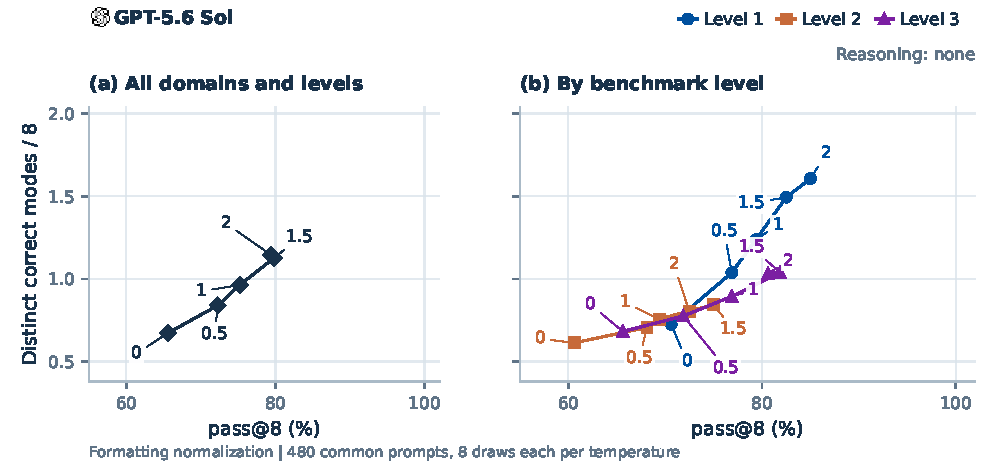
\includegraphics[width=.98\linewidth]{figures/gpt56_temperature_curve.pdf}
  \caption{\textbf{Nonzero temperatures yield greater observed eight-draw coverage.}
  GPT-5.6 Sol with reasoning \texttt{none}, typography normalization, and the same
  480 prompts at each of five temperatures (32 per domain--level cell, eight
  responses each). Left: an equal mean over all 15 domain--level cells; right:
  equal means over five domains at each level, identified by color and marker.
  The horizontal axis is empirical \texttt{pass@8}; the vertical axis averages
  distinct correct solution modes per eight responses, including unsolved prompts
  as zero. Labels give requested temperatures; segments connect measured point
  estimates in temperature order. Table~\ref{tab:gpt56-temperature} gives
  95\% whole-prompt bootstrap intervals. Mode counts depend on
  success and correct-answer variation and need not track \texttt{pass@8}.}
  \label{fig:gpt56-temperature-curve}
\end{figure}
}

\section{Comparison across Hosted Deployments}
\label{app:hosted-comparison}

Figure~\ref{fig:hosted-verified-breadth} compares accuracy and success-conditional
solution-mode diversity across hosted deployments. Its accuracy row uses a
common formatting normalizer and the revised Opus 5 \texttt{Python} instructions at
each level; hollow marks show that deployment's original \texttt{Python} condition.
Other accuracy cells use the original instructions. The diversity row uses
strict grades and original instructions for every deployment, with the
prompt-level estimand and eligibility criteria of App.~\ref{app:hosted-mode-diversity}.
Accuracy includes every response, including refusals and verification failures.
Provider settings differ, so the figure describes the stated configurations
rather than ranking models under matched prompts and compute.

The tables and \texttt{Graph} figure use the original instructions for every deployment.
The \texttt{Python} comparison reports both instruction conditions under strict and
formatting-normalized grading. Level 3 extends the evaluation beyond the
training levels, and difficulty need not increase with level for every hosted deployment.

\input{results/frontier_comparison_20260911_protocol.tex}
\input{results/frontier_comparison_20260911_graph_figure.tex}
\input{results/frontier_comparison_20260911_python_sensitivity.tex}
\input{results/frontier_python_retry_20260911.tex}

\input{results/frontier_temperature_20260911.tex}

\input{results/gpt56_temperature_curve_20260911_appendix.tex}
\input{results/frontier_comparison_20260911_provider_outcomes.tex}

\begin{table}[!htbp]
  \centering
  \caption{\textbf{Hosted deployments average fewer than three distinct correct modes per prompt.}
  Each row averages five domains equally under strict grading and original
  instructions, with 128 prompts per domain and eight responses per prompt.
  M/P are \texttt{mean@8}/\texttt{pass@8} (\%); D averages distinct correct
  solution modes, including zeros. C is correct-pair collision (\%), pooling
  pairs within each domain before averaging domains. Pointwise 95\% intervals
  use 2,000 whole-prompt bootstrap resamples within domains. A dash denotes
  an undefined domain collision and hence an undefined five-domain mean.
  Provider settings differ, so these are descriptive deployment comparisons.}
  \small
  \setlength{\tabcolsep}{3pt}
  \begin{tabular}{@{}lrrrrr@{}}
    \toprule
    Deployment & Level & M & P & D & C (95\% interval) \\
    \midrule
    \input{results/frontier_comparison_20260911_strict_overview_rows.tex}
  \end{tabular}
\end{table}

\input{results/frontier_comparison_20260911_strict_cells.tex}
\input{results/frontier_comparison_20260911_normalized_cells.tex}



% Generated by ops/build_paper_hosted_level_averages.py; do not edit.
\begin{table}[H]
  \centering
  \small
  \setlength{\tabcolsep}{4pt}
  \resizebox{\linewidth}{!}{%
  \begin{tabular}{lrrrrrrrrr}
    \toprule
    & \multicolumn{3}{c}{Level 1} & \multicolumn{3}{c}{Level 2} & \multicolumn{3}{c}{Level 3} \\
    \cmidrule(lr){2-4}\cmidrule(lr){5-7}\cmidrule(lr){8-10}
    Model & \texttt{pass@8} (\%) & \# modes & \pmd{} & \texttt{pass@8} (\%) & \# modes & \pmd{} & \texttt{pass@8} (\%) & \# modes & \pmd{} \\
    \midrule
    \raisebox{-0.15em}{
\includegraphics[width=1.05em,height=1.05em,keepaspectratio]{icons/openai.png}}\hspace{0.4em}GPT-5.6 Sol & 98.0 & 1.80 & .256 & 98.4 & 1.50 & .229\textsuperscript{\textdagger} & 99.2 & 1.45 & .183\textsuperscript{\textdagger} \\
    \raisebox{-0.15em}{
\includegraphics[width=1.05em,height=1.05em,keepaspectratio]{icons/claude.png}}\hspace{0.4em}Claude Opus 5 & 98.3\textsuperscript{\ensuremath{\ddagger}} & 1.43\textsuperscript{\ensuremath{\ddagger}} & .140 & 99.7\textsuperscript{\ensuremath{\ddagger}} & 1.44\textsuperscript{\ensuremath{\ddagger}} & .164\textsuperscript{\textdagger} & 99.8\textsuperscript{\ensuremath{\ddagger}} & 1.36\textsuperscript{\ensuremath{\ddagger}} & .121\textsuperscript{\textdagger} \\
    \raisebox{-0.15em}{
\includegraphics[width=1.05em,height=1.05em,keepaspectratio]{icons/openai.png}}\hspace{0.4em}GPT-5.4 & 98.1 & 2.11 & .338 & 98.4 & 1.72 & .247 & 99.5 & 1.68 & .224 \\
    \raisebox{-0.15em}{
\includegraphics[width=1.05em,height=1.05em,keepaspectratio]{icons/grok_official_docs_print.png}}\hspace{0.4em}Grok 4.3 & 99.5 & 1.97 & .275 & 100.0 & 1.57 & .179 & 100.0 & 1.55 & .171 \\
    \raisebox{-0.15em}{
\includegraphics[width=1.05em,height=1.05em,keepaspectratio]{icons/kimi.png}}\hspace{0.4em}Kimi K3 & 98.4 & 2.31 & .374 & 100.0 & 2.05 & .307 & 100.0 & 1.90 & .253 \\
    \raisebox{-0.15em}{
\includegraphics[width=1.05em,height=1.05em,keepaspectratio]{icons/claude.png}}\hspace{0.4em}Claude Opus 4.8 & 98.8 & 1.64 & .217 & 100.0 & 1.67 & .229 & 99.8 & 1.51 & .168 \\
    \raisebox{-0.15em}{
\includegraphics[width=1.05em,height=1.05em,keepaspectratio]{icons/deepseek.png}}\hspace{0.4em}DeepSeek V4 Pro & 98.4 & 2.01 & .289 & 99.1 & 1.84 & .319 & 99.7 & 1.62 & .232 \\
    \bottomrule
  \end{tabular}}
  \caption{\textbf{High prompt success coexists with few verified solution modes.}
  Each deployment requests medium reasoning effort, with 128 prompts per domain
  and level and eight responses per prompt. \texttt{pass@8} and \# modes use
  formatting-normalized grading and average the five domains equally:
  \texttt{pass@8} is empirical prompt success; \# modes is mean
  \texttt{distinct@8}, including zero for prompts without a verified response.
  \textsuperscript{\ensuremath{\ddagger}} marks the three Claude Opus 5 cells using
  revised \texttt{Python} wording without a system message (App.~\ref{app:hosted-python-prompt}).
  \pmd{} instead uses strict grading and the original wording throughout,
  averaging per-prompt diversity over prompts with at least two verified draws
  and then equally over reportable domains. These are the per-level columns of
  Table~\ref{tab:hosted-cohort-mode-diversity}, not its common-cell macro.
  \textsuperscript{\textdagger} marks four cells omitting \texttt{Python} because fewer
  than thirty prompts qualify: GPT-5.6 Sol has strict-formatting failures;
  Opus 5 has provider refusals. All entries are point estimates.
  Table~\ref{tab:hosted-level-averages-parity} gives normalized success and mode
  counts on the four domains with common wording.}
  \label{tab:hosted-level-averages-medium}
\end{table}


\begin{figure}[!htbp]
  \centering
  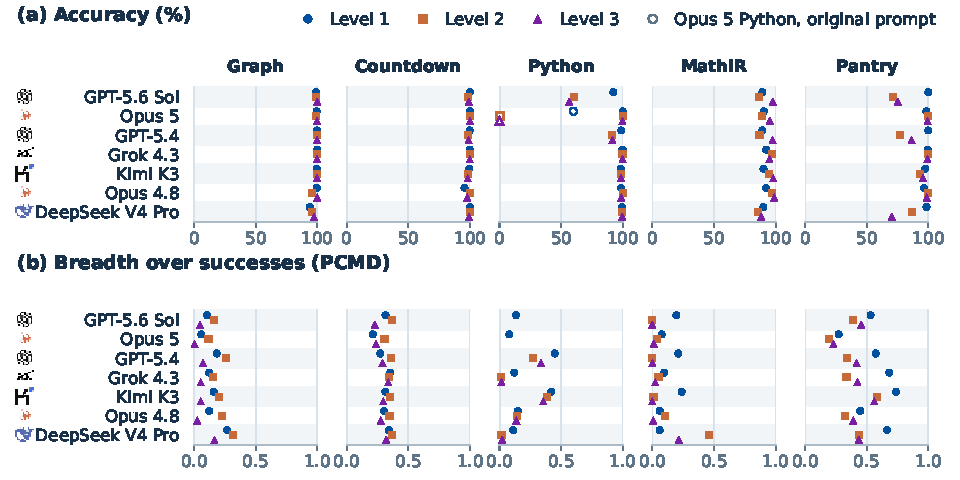
\includegraphics[width=\linewidth]{figures/hosted_verified_breadth.pdf}
  \caption{\textbf{Accurate hosted responses can still concentrate on few solution modes.}
  Columns show domains; colors and marker shapes distinguish Levels~1--3.
  Each deployment--domain--level cell uses 128 prompts and eight responses
  per prompt. Top: formatting-normalized response accuracy. Solid Opus~5
  \texttt{Python} marks use revised task wording without a system message; hollow marks
  show original wording. Bottom: promptwise \pmd{} under strict grading
  and original wording for every deployment, averaging over prompts with
  at least two verified draws. Cells with fewer than thirty eligible prompts
  are omitted. Thus the two rows use different grading and, for Opus~5
  \texttt{Python}, different prompt conditions. All marks are point estimates.
  Table~\ref{tab:hosted-level-averages-medium} gives per-level means;
  Table~\ref{tab:hosted-level-averages-parity} gives normalized success and
  mode counts on the four domains with common wording.}
  \label{fig:hosted-verified-breadth}
\end{figure}

% Generated by ops/build_paper_hosted_level_averages.py; do not edit.
\paragraph{Evaluation parity across deployments.}
One column of this cohort rests on wording the other deployments did not
answer: Claude Opus 5's Python cells in Fig.~\ref{fig:hosted-verified-breadth}
and Table~\ref{tab:hosted-level-averages-medium} use the revised condition of
App.~\ref{app:hosted-python-prompt}. Every other reading in this paper holds one
prompt across all seven deployments, including the \pmd{} column beside them,
Table~\ref{tab:hosted-cohort-mode-diversity} and the strict and normalized cell
tables above. Table~\ref{tab:hosted-level-averages-parity} therefore repeats the
comparison over Graph, Countdown, MathIR and Pantry alone, the four domains that share
one prompt. Claude Opus 5 averages
1.42/1.45/1.35 verified modes there at Levels 1--3,
against 1.43/1.44/1.36 over five domains with the
revised Python cell and 1.36/1.17/1.08
with the original one. It is the least varied deployment at every level under all
three readings, and the revised wording raises its Python breadth rather than
lowering it, so the substituted cell moves the five-domain reading away from
concentration rather than towards it. Which of the other six follows it varies
with Python in or out, as their per-domain disagreement in
Table~\ref{tab:hosted-cohort-mode-diversity} already reports; what survives every
reading is the level, not the order.
How far a Python wording change can carry this domain is itself measured, on
three of the other six: App.~\ref{app:sampling-budget-effects}
answers Python under two wordings at 16 prompts and
64 draws, and pooled \pmd{} moves by between
+.024 and +.131 across its
six deployment--level cells, leaving every one of them concentrated
under both wordings (highest \pmd{} .369,
$\neff$ 1.58). That bounds how far wording carries
this domain; it does not identify what this particular revision would do to a
deployment other than the one that answered it.

\begin{table}[H]
  \centering
  \small
  \setlength{\tabcolsep}{5pt}
  \begin{tabular}{lrrrrrr}
    \toprule
    & \multicolumn{2}{c}{Level 1} & \multicolumn{2}{c}{Level 2} & \multicolumn{2}{c}{Level 3} \\
    \cmidrule(lr){2-3}\cmidrule(lr){4-5}\cmidrule(lr){6-7}
    Model & \texttt{pass@8} (\%) & \# modes & \texttt{pass@8} (\%) & \# modes & \texttt{pass@8} (\%) & \# modes \\
    \midrule
    GPT-5.6 Sol & 97.5 & 1.90 & 98.2 & 1.59 & 99.4 & 1.54 \\
    Claude Opus 5 & 97.9 & 1.42 & 99.6 & 1.45 & 99.8 & 1.35 \\
    GPT-5.4 & 97.7 & 2.00 & 98.0 & 1.68 & 99.4 & 1.62 \\
    Grok 4.3 & 99.4 & 2.12 & 100.0 & 1.70 & 100.0 & 1.68 \\
    Kimi K3 & 98.0 & 2.26 & 100.0 & 1.95 & 100.0 & 1.79 \\
    Claude Opus 4.8 & 98.4 & 1.70 & 100.0 & 1.75 & 99.8 & 1.56 \\
    DeepSeek V4 Pro & 98.0 & 2.16 & 98.8 & 2.04 & 99.6 & 1.75 \\
    \bottomrule
  \end{tabular}
  \caption{\textbf{Hosted success and output diversity with Python excluded.}
  The same draws as Table~\ref{tab:hosted-level-averages-medium}, averaged over
  Graph, Countdown, MathIR and Pantry alone: the four domains every deployment answers
  under one prompt, 128 prompts each and eight responses per prompt. Reading this
  table beside that one shows what the revised Python condition of
  App.~\ref{app:hosted-python-prompt} carries, and what it does not.}
  \label{tab:hosted-level-averages-parity}
\end{table}


% Generated by ops/build_paper_gpt56sol_python_parity.py; do not edit.
\subsection{The revised \texttt{Python} wording on a second deployment}
\label{app:python-wording-second-deployment}

The original and revised \texttt{Python} conditions of App.~\ref{app:hosted-python-prompt}
are evaluated on GPT-5.6 Sol through \path{api.openai.com}. Each condition uses
the same 384 problems, with 128 prompts per level and eight responses per prompt,
medium reasoning effort and an 8,192-token output cap. The original condition
uses the benchmark request; the revised condition asks for a direct expression
without a system message. Public task inputs, allowed operators and the verifier
are unchanged, but wording and system-message presence change together.
Every response reports the model \texttt{gpt-5.6-sol}, but this build cannot be
shown to match the Azure deployment used for the hosted averages, so the two
are treated as separate populations.

\paragraph{Verified success and mode counts decrease under the revised condition.}
There are no provider-declared refusals among the
6,144 responses in this comparison.
The Azure GPT-5.6 Sol cohort also contains no provider-declared refusals;
its missing strict \texttt{Python} diversity entries reflect too few verified draws.
Under normalized grading, the revised condition lowers accuracy and mean
\texttt{distinct@8} at each level (Table~\ref{tab:gpt56sol-python-parity}).
Revised-minus-original differences use all 128 prompts per level, pairing
problems across conditions and resampling whole eight-response groups:
20,000 replicates give pointwise 95\% percentile intervals.
Accuracy differences are fractions of responses; mode-count differences are
modes per prompt:
accuracy $-.689$ $[-.745, -.631]$, $-.420$ $[-.467, -.374]$, $-.370$ $[-.418, -.320]$ at Levels 1--3;
\texttt{distinct@8} $-.945$ $[-1.078, -.820]$, $-.703$ $[-.812, -.594]$, $-.656$ $[-.766, -.547]$ respectively.
The revised normalized cells have
28, 26, 25
prompts with at least two verified responses, all below the 30-prompt
reporting threshold, so their success-conditional diversity and any diversity
contrast are omitted.

\paragraph{Formatting failures accompany the lower scores.}
The literal \LaTeX{} marker \verb|\text{| appears in
862 original-condition and
2,089 revised-condition responses
(28\% and 68\%).
The formatting normalizer does not remove this wrapper; none of these responses
verifies. Among responses without the marker, normalized success is
94.9\% and 59.3\%, respectively.
Absence of this marker does not guarantee parseability. Because the marker
depends on the response, these subsets are not matched comparisons and do not
bound a content or capability effect.

\paragraph{Prompt-interface sensitivity differs across deployments.}
The revised condition increases normalized success and verified mode counts
for Opus 5 (App.~\ref{app:hosted-python-prompt}) but decreases both for this
GPT-5.6 Sol deployment. This comparison does not isolate task wording from the
system message, establish that either task is generally easier, or identify
the effect on the remaining hosted deployments. The four-domain comparison in
Table~\ref{tab:hosted-level-averages-parity} holds the task prompts fixed across
all seven deployments by excluding \texttt{Python}.

\begin{table}[!htbp]
  \centering
  \caption{\textbf{The revised \texttt{Python} condition lowers normalized success and verified mode counts on GPT-5.6 Sol.}
  Both conditions use the same 128 problems per level and eight responses per
  prompt through \texttt{api.openai.com}, with medium reasoning effort and an
  8,192-token output cap. R counts provider-declared refusals; A is response
  accuracy (\%); D is mean \texttt{distinct@8} over all prompts.
  $1-C$ is pair-pooled diversity: the fraction of correct pairs with different
  solution modes, weighting each correct pair equally across prompts.
  Dashes mark cells with fewer than 30 prompts containing at least two
  verified draws. Strict grading uses the original output; normalized grading
  applies the same typography rules to both conditions. Entries are point
  estimates; paired uncertainty for accuracy and mode-count differences is
  given in the surrounding text.}
  \small
  \setlength{\tabcolsep}{4pt}
  \begin{tabular}{@{}llrrrrrrr@{}}
    \toprule
    & & & \multicolumn{3}{c}{Strict} & \multicolumn{3}{c}{Normalized} \\
    \cmidrule(lr){4-6}\cmidrule(lr){7-9}
    Wording & L & R & A & D & $1-C$ & A & D & $1-C$ \\
    \midrule
    Original & 1 & 0 & 37.0 & 1.02 & .106 & 89.8 & 1.36 & .114 \\
     & 2 & 0 & 10.4 & 0.14 & --- & 58.7 & 1.15 & .053 \\
     & 3 & 0 & 13.0 & 0.16 & --- & 56.3 & 1.13 & .048 \\
    \midrule
    Revised, no system & 1 & 0 & 18.7 & 0.27 & --- & 20.9 & 0.41 & --- \\
     & 2 & 0 & 13.4 & 0.26 & --- & 16.7 & 0.45 & --- \\
     & 3 & 0 & 15.5 & 0.25 & --- & 19.3 & 0.48 & --- \\
    \bottomrule
  \end{tabular}
  \label{tab:gpt56sol-python-parity}
\end{table}


% Generated by ops/build_paper_hosted_reasoning_off.py; do not edit.
\begin{table}[H]
  \centering
  \small
  \setlength{\tabcolsep}{5pt}
  \begin{tabular}{lrrrrrr}
    \toprule
    & \multicolumn{2}{c}{Level 1} & \multicolumn{2}{c}{Level 2} & \multicolumn{2}{c}{Level 3} \\
    \cmidrule(lr){2-3}\cmidrule(lr){4-5}\cmidrule(lr){6-7}
    Model & \texttt{pass@8} (\%) & \# modes & \texttt{pass@8} (\%) & \# modes & \texttt{pass@8} (\%) & \# modes \\
    \midrule
    \raisebox{-0.15em}{
\includegraphics[width=1.05em,height=1.05em,keepaspectratio]{icons/openai.png}}\hspace{0.4em}GPT-5.6 Sol & 82.5 & 1.31 & 66.9 & 0.76 & 76.2 & 0.88 \\
    \raisebox{-0.15em}{
\includegraphics[width=1.05em,height=1.05em,keepaspectratio]{icons/openai.png}}\hspace{0.4em}GPT-5.4 & 82.5 & 1.67 & 71.2 & 0.92 & 70.0 & 0.94 \\
    \raisebox{-0.15em}{
\includegraphics[width=1.05em,height=1.05em,keepaspectratio]{icons/grok_official_docs_print.png}}\hspace{0.4em}Grok 4.3 & 82.5 & 1.64 & 86.9 & 1.41 & 90.0 & 1.45 \\
    \raisebox{-0.15em}{
\includegraphics[width=1.05em,height=1.05em,keepaspectratio]{icons/kimi.png}}\hspace{0.4em}Kimi K3 & 92.5 & 1.91 & 92.5 & 1.37 & 95.6 & 1.59 \\
    \raisebox{-0.15em}{
\includegraphics[width=1.05em,height=1.05em,keepaspectratio]{icons/claude.png}}\hspace{0.4em}Claude Opus 4.8 & 91.2 & 1.46 & 100.0 & 1.62 & 100.0 & 1.51 \\
    \bottomrule
  \end{tabular}
  \caption{\textbf{Hosted success and output diversity with reasoning disabled.}
  Each level averages five domains equally: 32 prompts per domain and eight
  responses per prompt. \texttt{pass@8} is the fraction with any verified
  response; \# modes is mean \texttt{distinct@8}, including failures.
  The frozen formatting normalizer applies throughout. Appendix~\ref{app:hosted-reasoning-control}
  gives matched medium-reasoning results.}
  \label{tab:hosted-level-averages}
\end{table}


% Generated by ops/build_paper_hosted_reasoning_off.py; do not edit.
\subsection{Matched reasoning-control comparison}
\label{app:hosted-reasoning-control}
We selected original row indices 0--31 in each of five domains and three
levels, without consulting outputs. Each model and condition therefore has
480 prompts and 3,840 responses. The medium baseline reuses the original
audited responses for these exact prompts and eight sample slots; no new
medium responses were collected. Both conditions preserve the original
system and user prompt bytes, including the original Python wording.
The 128-prompt medium results in Table~\ref{tab:hosted-level-averages-medium}
and Figure~\ref{fig:hosted-verified-breadth} are a separate, larger display;
the comparison below uses only the matched 32-prompt subset.

Only the provider reasoning control changes, with an 8,192-token output
budget retained in both conditions. GPT-5.6 Sol and GPT-5.4 request
\texttt{reasoning.effort=none}; Grok 4.3 and Kimi K3 request
\texttt{reasoning\_effort=none}. Claude Opus 4.8 requests
\texttt{thinking.type=disabled} while retaining
\texttt{output\_config.effort=medium}. These controls denote disabled
explicit reasoning at the endpoint, without establishing the absence of
hidden internal computation. Native response receipts are checked for
control violations. The same frozen formatting normalizer and canonical
mode grader apply to both conditions; the accompanying JSON retains strict
grades, domain-level counts, controls, and source hashes.

\begin{table}[H]
  \centering
  \small
  \setlength{\tabcolsep}{5pt}
  \begin{tabular}{llrrcrrc}
    \toprule
    & & \multicolumn{3}{c}{Medium reasoning} & \multicolumn{3}{c}{Reasoning disabled} \\
    \cmidrule(lr){3-5}\cmidrule(lr){6-8}
    Model & Level & \texttt{pass@8} (\%) & \# modes & \pmd{} & \texttt{pass@8} (\%) & \# modes & \pmd{} \\
    \midrule
    \raisebox{-0.15em}{
\includegraphics[width=1.05em,height=1.05em,keepaspectratio]{icons/openai.png}}\hspace{0.4em}GPT-5.6 Sol & 1 & 96.9 & 1.81 & .311 & 82.5 & 1.31 & .226 \\
     & 2 & 98.8 & 1.54 & .117 & 66.9 & 0.76 & .063 \\
     & 3 & 98.8 & 1.51 & .195 & 76.2 & 0.88 & .095 \\
    \cmidrule(l){2-8}
     & \textit{All} & 98.1 & 1.62 & .226 & 75.2 & 0.99 & .145 \\
    \addlinespace
    \raisebox{-0.15em}{
\includegraphics[width=1.05em,height=1.05em,keepaspectratio]{icons/openai.png}}\hspace{0.4em}GPT-5.4 & 1 & 96.9 & 2.06 & .338 & 82.5 & 1.67 & .347 \\
     & 2 & 99.4 & 1.68 & .162 & 71.2 & 0.92 & .134 \\
     & 3 & 99.4 & 1.82 & .247 & 70.0 & 0.94 & .160 \\
    \cmidrule(l){2-8}
     & \textit{All} & 98.5 & 1.85 & .255 & 74.6 & 1.18 & .224 \\
    \addlinespace
    \raisebox{-0.15em}{
\includegraphics[width=1.05em,height=1.05em,keepaspectratio]{icons/grok_official_docs_print.png}}\hspace{0.4em}Grok 4.3 & 1 & 100.0 & 1.93 & .211 & 82.5 & 1.64 & .493 \\
     & 2 & 100.0 & 1.62 & .136 & 86.9 & 1.41 & .296 \\
     & 3 & 100.0 & 1.54 & .121 & 90.0 & 1.45 & .314 \\
    \cmidrule(l){2-8}
     & \textit{All} & 100.0 & 1.70 & .154 & 86.5 & 1.50 & .364 \\
    \addlinespace
    \raisebox{-0.15em}{
\includegraphics[width=1.05em,height=1.05em,keepaspectratio]{icons/kimi.png}}\hspace{0.4em}Kimi K3 & 1 & 96.9 & 2.27 & .343 & 92.5 & 1.91 & .595 \\
     & 2 & 100.0 & 2.02 & .277 & 92.5 & 1.37 & .335 \\
     & 3 & 100.0 & 1.89 & .264 & 95.6 & 1.59 & .361 \\
    \cmidrule(l){2-8}
     & \textit{All} & 99.0 & 2.06 & .293 & 93.5 & 1.62 & .426 \\
    \addlinespace
    \raisebox{-0.15em}{
\includegraphics[width=1.05em,height=1.05em,keepaspectratio]{icons/claude.png}}\hspace{0.4em}Claude Opus 4.8 & 1 & 98.1 & 1.61 & .202 & 91.2 & 1.46 & .216 \\
     & 2 & 100.0 & 1.67 & .218 & 100.0 & 1.62 & .226 \\
     & 3 & 100.0 & 1.57 & .185 & 100.0 & 1.51 & .185 \\
    \cmidrule(l){2-8}
     & \textit{All} & 99.4 & 1.62 & .202 & 97.1 & 1.53 & .209 \\
    \bottomrule
  \end{tabular}
  \caption{\textbf{Matched medium and disabled reasoning, by level.}
  Each row averages 160 prompts across five domains. All eight responses
  and zero-success prompts are retained. \# modes denotes mean
  \texttt{distinct@8}; estimates use the frozen formatting normalizer.
  \pmd{} is paired within the level: it averages over the prompts of that
  level which return two verified draws in both conditions, between
  65 and 159 of the 160 per cell, and every level cell here clears the
  thirty-prompt support bar.
  The \texttt{pass@8} and \# modes columns use all 160 prompts, so the two
  axes are read on the same draws but not on the same denominators, and the
  paired count behind every level cell is retained in the accompanying
  machine-readable record alongside the per-domain counts.
  The \textit{All} row averages the same 480 prompts and 3,840 responses
  per condition with equal weight on every domain and level; its \pmd{}
  is the paired reading over the
  245--458 prompts per deployment that return two verified draws in both conditions.
  That column separates concentration from lost accuracy, since a prompt
  one condition stopped answering twice leaves the estimate rather than
  entering it as a smaller number; the per-domain readings behind it are
  retained in the accompanying JSON, together with the prompts that only
  one of the two conditions answers twice and so enter neither average.}
  \label{tab:hosted-reasoning-matched-levels}
\end{table}

\paragraph{Incomplete deployments.}
Five of seven registered deployments passed complete-cohort admission,
and neither partial cohort receives a score. They fall short in different
ways, and that decides what can still be read from each.

DeepSeek V4 Pro's draws are intact, so its measurement survives its
exclusion and is reported here: read on the 437 prompts both of its
conditions define, disabling reasoning moves \pmd{} from
$.282$ to $.369$, a change of $+.087$. What that figure
cannot do is join the table, for two reasons and neither is the recovery
shortfall: both of its arms are graded strictly, because the frozen
normalizer was only ever run on admitted cohorts, and one PantryPlan prompt
holds seven draws rather than eight. A caveat cannot put a strictly graded
number on the same scale as a normalized one. The shortfall itself is
slight --- 3,839 of 3,840 sample receipts were recovered, leaving one
unresolved request, which is not counted as a failure --- and it is not
what keeps the deployment out of the table. The figure is reported so the
evidence is not lost, not so it can be compared.

Claude Opus 5 admits no such reading. A native response returned a thinking
block and 40 thinking tokens despite an explicit disabled-thinking request,
so its disabled condition did not disable reasoning. There is no
reasoning-off measurement to preserve, rather than one withheld.

\paragraph{Scope of the comparison.}
Across all five complete deployments, disabling reasoning lowers both
overall \texttt{pass@8} and observed \distk{}. Reduced success also
reduces opportunities to observe distinct successful modes, so those two
columns cannot separate concentration from lost accuracy. \pmd{} can, and
the answer is not uniform: on the prompts both conditions define, breadth
falls for GPT-5.6 Sol and GPT-5.4, is unchanged for Claude Opus 4.8, and
rises for Kimi K3 and Grok 4.3, which more than doubles from $.154$ to
$.364$ while its \distk{} falls. Disabling deliberation concentrates some
deployments and spreads others, so the common fall in \distk{} tracks the
accuracy drop rather than a shared collapse.
Table~\ref{tab:hosted-reasoning-matched-levels} reads the same contrast at
each level, and the direction belongs to the deployment rather than to the
level: GPT-5.6 Sol falls at every level, Grok 4.3 and Kimi K3 rise at
every level, GPT-5.4 is flat at Level 1 and falls at Levels 2 and 3, and
Claude Opus 4.8 stays within $.014$ of zero throughout.
No deployment reverses its own direction from one level to the next, and
no level cell loses the measurement: every one clears the support bar on
prompts both conditions answer twice. Medium and disabled outputs
were collected at different times; matching sample slots are not shared
random seeds. Omitted temperature and \texttt{top\_p} controls retain
provider defaults, which can vary over time. These are descriptive point
estimates without uncertainty intervals, not causal claims about training.


\clearpage
\phantomsection
\begin{center}\large\textbf{Part VI. Idealized analysis}\end{center}
\addcontentsline{toc}{part}{Part VI. Idealized analysis}

\section{Mode Collapse and Verified Replay}
\label{app:theory}

This part collects the idealized analysis behind
Section~\ref{sec:collapse-mechanism}. The winner-take-all limit of
binary-reward policy gradient among equally rewarded outcomes is established
by \citet{sinha2026expected} and \citet{lochab2026ucpo} and is a replicator
system in the sense of \citet{hofbauer1998evolutionary}; we restate it in our
categorical model so that the later statements share its notation, and we do
not reprove it. What this part adds is: an exact identity showing that every
outcome-binary advantage induces the same conditional trajectory, so the
choice among Dr.GRPO, GRPO, and MaxRL rescales time without changing which
mode survives; a starvation bound showing that fresh groups supply no gradient
to a rare mode as its probability vanishes, whereas a fixed verified buffer
does; a uniform-in-time probability floor for every buffered mode under a
fixed replay dose, with the coupon-collection ordering that makes uniform
allocation optimal for finite-budget coverage; and the stationary target of a
reference-KL anchor, whose conditional allocation is the reference's. Every
statement is for one isolated prompt with independent categorical logits and
Euclidean expected-gradient flow. These results do not certify the
implemented AdamW/PPO trajectories. The final subsection states where the
assumptions stop and which signs and orderings the runs were checked against.
Table~\ref{tab:notation} defines the notation.

\subsection{Categorical model, and the known winner-take-all limit}
\label{app:theory-grpo-mean}
\label{app:theory-collapse}
\label{app:theory-objective-inertness}

The categorical model assigns one independent logit to each outcome
category. Its Euclidean mean flow and the subsequent finite-step, sampled,
and neural updates have different assumptions; a neural solution mode need
not have an independently optimized logit.

\begin{assumption}[Categorical mean-flow model]
\label{ass:categorical-mean-flow}
Fix one isolated prompt and a finite category set
$\mathcal A=\mathcal C\mathbin{\dot\cup}\mathcal N$ with $m\ge2$ correct
solution modes and $n\ge1$ incorrect categories, and set
$p_a=\operatorname{softmax}(z)_a$, $P=\sum_{c\in\mathcal C}p_c$, and
$q_c=p_c/P$, so that $P$ measures correctness while $q$ describes how that
correct probability is allocated among the individual correct modes.
\begin{enumerate}
\item[(A1)] \emph{Independent logits.} The policy carries one independently
  optimized logit for every category in $\mathcal A$, including one separate
  logit for each canonical correct mode.
\item[(A2)] \emph{Common length normalization.} Every response uses the same
  fixed length-normalization factor, absorbed into the positive coefficient
  of the group estimator.
\item[(A3)] \emph{Euclidean mean flow.} Updates are the infinitesimal expected
  updates in these logits, taken without optimizer preconditioning and without
  momentum carried between steps.
\item[(A4)] \emph{No competing regularizer.} Explicit reference KL is zero and
  no entropy term is present.
\item[(A5)] \emph{Nondegenerate start.} Logits are finite initially,
  $0<P(0)<1$, and the group size is $G\ge2$.
\end{enumerate}
\end{assumption}

Assumption~\ref{ass:categorical-mean-flow} comprises conditions (A1)--(A5).
AdamW's preconditioning and momentum violate (A3); finite, repeated PPO
updates are outside its infinitesimal on-policy limit. Response-specific
length normalization violates (A2), while reference KL and entropy
regularization violate (A4).

A language model induces probabilities over canonical outcomes, but those
probabilities alone do not determine its update geometry. Aggregating several
response strings into a mode does not generally commute with gradient flow
in response logits. The independent-category model therefore requires an
additional assumption beyond a neural policy and its validator equivalence
classes.

Draw a group $Z_1,\ldots,Z_G\stackrel{\mathrm{iid}}{\sim}p$ with $G\ge2$,
write $R_i=\1[Z_i\in\mathcal C]$, and let $R=\sum_iR_i$. At the on-policy
point where the PPO ratio equals one, consider the common-length estimator
\begin{equation}
  \widehat g_G
  =\frac1G\sum_{i=1}^G
   w(R)\left(R_i-\frac{R}{G}\right)\nabla_z\log p_{Z_i}.
  \label{eq:group-estimator}
\end{equation}
For the Dr.GRPO abstraction \citep{liu2025understanding}, $w(R)=1$ after
absorbing the fixed positive length-normalization factor. Reward-standardized
GRPO \citep{shao2024deepseekmath} with fixed common response-length
normalization takes $w(R)$ to be the reciprocal group reward standard
deviation on mixed groups (with a fixed numerical stabilizer if used).
Standard variable-length GRPO also weights each response by its own inverse
length; that response-specific factor cannot generally be absorbed into
$w(R)$ and is outside this equivalence.
In both cases, $0<w(\ell)<\infty$ for
$\ell\in\{1,\ldots,G-1\}$. The entire update is zero on all-equal
groups, without evaluating an undefined reciprocal standard deviation;
likewise, $w(R)R(G-R)$ below is defined as zero when $R=0$ or $R=G$. All
advantages and normalization weights are detached in the score estimator.

\begin{lemma}[A group baseline does not remove frequency amplification]
\enforcehalffinalproseline
\label{lem:grpo-mean}
For $0<P<1$, the expected update in Equation~\eqref{eq:group-estimator} is
\begin{equation}
  \E[\widehat g_G]
  =c_G(P)\nabla_z P,
  \qquad
  c_G(P)=
  \frac{\E\!\big[w(R)R(G-R)\big]}{G^2P(1-P)}>0.
  \label{eq:expected-group-gradient}
\end{equation}
For the Dr.GRPO abstraction, $c_G(P)=(G-1)/G$. Group centering and reward
standardization rescale the expected gradient without changing its direction
under these assumptions.
\end{lemma}

\begin{proof}
\enforcehalffinalproseline
Condition on the complete binary reward vector, whose sum is $R$. The score
identities give
\[
  \E[\nabla_z\log p_{Z_i}\mid R_i=1]=\nabla_z\log P,
  \qquad
  \E[\nabla_z\log p_{Z_i}\mid R_i=0]
  =\nabla_z\log(1-P).
\]
There are $R$ correct rows with centered reward $(G-R)/G$ and $G-R$
incorrect rows with centered reward $-R/G$. Therefore the conditional
expectation of the unaveraged sum in~\eqref{eq:group-estimator} is
\[
  w(R)\frac{R(G-R)}{G}
  \left(\nabla_z\log P-\nabla_z\log(1-P)\right)
  =w(R)\frac{R(G-R)}{GP(1-P)}\nabla_zP.
\]
The outer factor $1/G$ and expectation over
$R\sim\operatorname{Binomial}(G,P)$ yield~\eqref{eq:expected-group-gradient}.
For $w\equiv1$,
$\E[R(G-R)]=G(G-1)P(1-P)$, proving the Dr.GRPO value.
\end{proof}

The binomial identity also gives the denominator-free expression
\[
 c_G(P)=\frac{G-1}{G}\sum_{j=0}^{G-2}\binom{G-2}{j}
 w(j+1)P^j(1-P)^{G-2-j}.
\]
The binomial weights sum to one, so $c_G$ lies between
$(G-1)\min_j w(j+1)/G$ and $(G-1)\max_j w(j+1)/G$.
Thus $c_G$ extends smoothly and positively to $P=0,1$.

The practical MaxRL estimator has the same mean-gradient direction
\citep[Section~4.3 and App.~D, Theorem~5]{tajwar2026maxrl}. Its all-failure
convention determines the finite-group coefficient.

\begin{lemma}[Binary MaxRL has the same correctness-gradient direction]
\enforcehalffinalproseline
\label{lem:maxrl-mean}
Under Assumption~\ref{ass:categorical-mean-flow}, let MaxRL assign
$A_i^{\mathrm{MaxRL}}=GR_i/R-1$ when $R>0$ and zero when $R=0$, as in
Section~\ref{app:binary-maxrl}. For
$\widehat g_G^{\mathrm{MaxRL}}=G^{-1}\sum_i
 A_i^{\mathrm{MaxRL}}\nabla_z\log p_{Z_i}$ at the on-policy point, the
expected update is
\begin{equation}
  \E[\widehat g_G^{\mathrm{MaxRL}}]
  =c_G^{\mathrm{MaxRL}}(P)\nabla_zP,
  \qquad
  c_G^{\mathrm{MaxRL}}(P)
  =\frac{1-(1-P)^{G-1}}{P}>0,
  \label{eq:maxrl-expected-gradient}
\end{equation}
with continuous endpoint values
$c_G^{\mathrm{MaxRL}}(0)=G-1$ and
$c_G^{\mathrm{MaxRL}}(1)=1$.
\end{lemma}

\begin{proof}
\enforcehalffinalproseline
With $N=G$ and pass rate $P$, the estimator in
\citet[Theorem~5]{tajwar2026maxrl} equals
$\widehat g_G^{\mathrm{MaxRL}}$. Its expected coefficient is
$\sum_{j=0}^{G-2}(1-P)^j$, whose geometric sum gives
Equation~\eqref{eq:maxrl-expected-gradient} and its endpoint values.
The identity requires on-policy independent draws and the score identity.
\end{proof}

Integrating this coefficient gives the potential
\begin{equation}
 \Psi_{\mathrm{MaxRL}}(P)
 :=\int_0^P c_G^{\mathrm{MaxRL}}(s)\,ds
 =\sum_{k=1}^{G-1}\frac{1-(1-P)^k}{k}.
 \label{eq:maxrl-potential-finite-sum}
\end{equation}
In particular, $\Psi_{\mathrm{MaxRL}}(1)=\sum_{k=1}^{G-1}1/k$.
For binary rewards, best@\(k\) equals pass@\(k\), so this is a harmonic
mixture of sampling objectives for $k=1,\ldots,G-1$. The upper limit is
$G-1$ because the implemented centered estimator sets the entire update
to zero on all-failure groups. Subtracting an unconditional score baseline
even on those groups instead gives the order-$G$ estimator. These are exact
finite-group expectations at the on-policy point; subsequent clipping and
adaptive optimization can alter the expected update.

\paragraph{Winner-take-all collapse.}
Consider $\dot z=c_G(P)\nabla_zP$, with any of the smooth positive
coefficients established above: Dr.GRPO, common-length reward-standardized
GRPO, or the specified centered binary MaxRL estimator. This infinitesimal
expected-update model has
no sampling noise and uses independently optimized Euclidean logits. The
conditional dynamics follow the frequency-dependent replicator system
with fitness $f_c(q)=q_c$
\citep{hofbauer1998evolutionary,harper2009informationgeometry}.
The limit below is the outcome-level collapse of
\citet[Theorem~3.1]{sinha2026expected} for softmax outcome logits, and the
indifference-plus-amplification mechanism of
\citet[Sections~4.1--4.2]{lochab2026ucpo}. We restate it in the present
notation and give only the reduction to the replicator flow, which is the
step the replay results reuse; it is not a new result.

\begin{proposition}[Winner-take-all collapse in the categorical mean flow]
\enforcehalffinalproseline
\label{thm:grpo-collapse}
Under Assumption~\ref{ass:categorical-mean-flow}, if the conditional correct-mode
distribution $q(0)$ has a unique largest coordinate $c^\star$, then
\[
  P(t)\longrightarrow1,
  \qquad
  q_{c^\star}(t)\longrightarrow1,
  \qquad
  q_c(t)\longrightarrow0\quad(c\ne c^\star).
\]
Thus these categorical mean flows converge to a single correct solution
mode for generic initial conditions, even though every mode in $\mathcal C$
has exactly the same reward.
\end{proposition}

\begin{proof}
\enforcehalffinalproseline
Since $\dot P=c_G(P)\lVert\nabla_zP\rVert_2^2$ with
$\lVert\nabla_zP\rVert_2^2\ge P^2(1-P)^2(1/m+1/n)$ and $c_G$ positive and
continuous on $[0,1]$, $P$ cannot converge to an interior value, so
$P\to1$. Define the effective time
$\tau(t)=\int_0^t c_G(P(s))P(s)(1-P(s))\,ds$. Every logit has absolute
velocity at most $\dot\tau$, so $\tau(\infty)<\infty$ would give every logit
finite total variation and a finite limit, contradicting $P\to1$; hence
$\tau\to\infty$. On the correct simplex the change of time gives
\begin{equation}
  \frac{dq_c}{d\tau}
  =q_c\left(q_c-\sum_{d\in\mathcal C}q_d^2\right),
  \qquad
  \frac{d}{d\tau}\log\frac{q_c}{q_d}=q_c-q_d,
  \label{eq:grpo-replicator}
\end{equation}
the replicator flow with fitness $f_c(q)=q_c$
\citep{hofbauer1998evolutionary}, which is the log-ratio dynamics of
\citet[Theorem~3.1]{sinha2026expected}. For $c\ne c^\star$ the ratio
$\xi_c=q_c/q_{c^\star}$ satisfies
$d\log\xi_c/d\tau=-q_{c^\star}(1-\xi_c)\le-(1-\xi_c(0))/m$, so every
competitor vanishes relative to the initial leader over infinite effective
time, and normalization gives $q_{c^\star}\to1$.
\end{proof}

If several modes tie for the largest initial probability, symmetry preserves
the tie; the same ratio argument eliminates strictly smaller coordinates and
leaves the tied maxima uniform. An exactly uniform correct distribution is
therefore a special initial condition. The theorem concerns limiting
concentration: finite softmax logits already give positive probabilities at
every finite time, so finite-time positivity alone is not a retention result.

\begin{remark}
Proposition~\ref{thm:grpo-collapse} is asymptotic and requires (A1)--(A5).
Finite-time support loss and convergence of the stochastic neural optimizers
used in the experiments are outside its scope.
\end{remark}

\paragraph{Every outcome-binary advantage follows the same conditional trajectory.}
Expected binary reward is the total correct mass and is indifferent to its
allocation among correct modes \citep[Section~4.1]{lochab2026ucpo}. The
following identity is the finite-group form used below: the choice among
Dr.GRPO, reward-standardized GRPO, a leave-one-out baseline, and centered
MaxRL rescales optimization time along the correctness axis without changing
the trajectory of $q$ or the identity of the surviving mode.

\begin{lemma}[Conditional inertness of outcome-binary objectives]
\label{thm:objective-inertness}
Under Assumption~\ref{ass:categorical-mean-flow}, let $a(\cdot,\cdot)$ be any
detached advantage measurable with respect to the group's binary reward
vector, applied as
$\widehat g_a=G^{-1}\sum_{i}a(R_i,R)\nabla_z\log p_{Z_i}$ at the on-policy
point. Then
\begin{equation}
  \E[\widehat g_a]=c_a(P)\,\nabla_zP,
  \qquad
  c_a(P)=\frac1G\left(
  \frac{\E[R\,a(1,R)]}{P}-\frac{\E[(G-R)\,a(0,R)]}{1-P}\right).
  \label{eq:objective-inertness}
\end{equation}
If $c_a>0$ on $(0,1)$, then under the time change
$d\tau=c_a(P)P(1-P)\,dt$ the conditional distribution $q$ obeys
Equation~\eqref{eq:grpo-replicator} exactly, for every such $a$. Dr.GRPO,
reward-standardized GRPO, a leave-one-out baseline, the centered binary MaxRL
estimator, and any reweighting shaped by a pass@$k$ target are points in this
class. The choice among them rescales optimization time along the correctness
axis and leaves both the trajectory in $q$ and the identity of the surviving
mode unchanged.
\end{lemma}

\begin{proof}
\enforcehalffinalproseline
The score identities used in Lemma~\ref{lem:grpo-mean} give
$\E[\nabla_z\log p_{Z_i}\mid R_i=1]=\nabla_z\log P$ and
$\E[\nabla_z\log p_{Z_i}\mid R_i=0]=\nabla_z\log(1-P)$.
Independence of the draws means that conditioning also on the other rows'
rewards does not change either conditional mean. Since $a(R_i,R)$ depends
only on the binary rewards, conditioning on their complete vector and
summing the $R$ successful and $G-R$ failed rows gives
\[
  \E[\widehat g_a]
  =\frac1G\Big(\E[R\,a(1,R)]\nabla_z\log P
   +\E[(G-R)\,a(0,R)]\nabla_z\log(1-P)\Big).
\]
Substituting $\nabla_z\log P=\nabla_zP/P$ and
$\nabla_z\log(1-P)=-\nabla_zP/(1-P)$ yields
Equation~\eqref{eq:objective-inertness}. Hence
$\frac{d}{dt}\log(q_c/q_d)=\dot z_c-\dot z_d=c_a(P)P(1-P)(q_c-q_d)$.
For $c_a>0$, the positive time change $d\tau=c_a(P)P(1-P)\,dt$ gives
the replicator dynamics in Equation~\eqref{eq:grpo-replicator}.
\end{proof}

For a fixed reward-dependent advantage, the binomial identities
$R\binom GR=G\binom{G-1}{R-1}$ and
$(G-R)\binom GR=G\binom{G-1}{R}$ give
\begin{equation}
 c_a(P)=\sum_{j=0}^{G-1}\binom{G-1}{j}P^j(1-P)^{G-1-j}
 \big[a(1,j+1)-a(0,j)\big],
 \label{eq:inertness-polynomial}
\end{equation}
a polynomial in $P$ of degree at most $G-1$. Finite advantage values
therefore give a smooth, bounded coefficient on $[0,1]$. This bounded coefficient is what the retention argument in
App.~\ref{app:theory-replay} uses.

\begin{corollary}[MaxRL amplification of the correctness gradient]
\enforcehalffinalproseline
\label{cor:maxrl-starvation}
For the coefficients of Lemmas~\ref{lem:grpo-mean} and~\ref{lem:maxrl-mean},
\[
 \frac{c_G^{\mathrm{MaxRL}}(P)}{c_G^{\mathrm{Dr.GRPO}}}
 =\frac{G\big[1-(1-P)^{G-1}\big]}{(G-1)P}.
\]
This ratio is nonincreasing in $P$, with limits $G$ as $P\to0$ and
$G/(G-1)$ as $P\to1$. It is strictly decreasing for $G>2$ and constant
at $2$ for $G=2$. At the same policy, MaxRL therefore multiplies the
Dr.GRPO correctness-gradient coefficient by a factor approaching $G$ when
correctness is small. The probability of a nonzero fresh task component
remains bounded by the mixed-group probability in
Lemma~\ref{lem:replay-gradient-availability} for both estimators.
\end{corollary}

\begin{proof}
\enforcehalffinalproseline
Divide $c_G^{\mathrm{MaxRL}}(P)=[1-(1-P)^{G-1}]/P$ by $(G-1)/G$.
The finite-series identity
$c_G^{\mathrm{MaxRL}}(P)=\sum_{j=0}^{G-2}(1-P)^j$
gives the endpoint limits and monotonicity. For $G=2$ the sum is the
constant $1$; for $G>2$ it contains the strictly decreasing term $1-P$.
\end{proof}

\subsection{A replay signal when fresh groups supply none}
\label{app:theory-gradient-availability}

\begin{lemma}[Fresh-group starvation]
\enforcehalffinalproseline
\label{lem:replay-gradient-availability}
Under Assumption~\ref{ass:categorical-mean-flow} with correctness probability
$P$, draw $G$ fresh categories independently. The probability of a
mixed-reward group is
\[
 h_G(P)=1-P^G-(1-P)^G\le G\min\{P,1-P\}.
\]
Every all-equal group has zero fresh task component for
Equation~\eqref{eq:group-estimator} and for the specified centered MaxRL
estimator, so the probability of a nonzero fresh task component is at most $h_G(P)$.
\end{lemma}

\begin{proof}
\enforcehalffinalproseline
The all-correct and all-incorrect events are disjoint and have probabilities
$P^G$ and $(1-P)^G$. A mixed group needs at least one correct and at least
one incorrect sample, so a union bound over the $G$ draws gives both
$h_G(P)\le GP$ and $h_G(P)\le G(1-P)$, and hence the stated minimum.
\end{proof}

\begin{lemma}[Replay ascent persists as fresh signal vanishes]
\enforcehalffinalproseline
\label{lem:replay-ascent}
Under Assumption~\ref{ass:categorical-mean-flow}, let
$\mathcal B\subseteq\mathcal C$ be a nonempty fixed verified buffer with
normalized positive weights $w_b$, let $R_w=-\sum_b w_b\log p_b$ with replay
coefficient $\rho_w>0$, and extend $w$ by zero outside the buffer to obtain $\bar w$. The
deterministic replay ascent vector is
\[
 v^{\rm replay}=-\rho_w\nabla R_w=\rho_w(\bar w-p),
\]
which vanishes only at $p=\bar w$. If $p_b\le w_b/2$ for a buffered mode, then
$v^{\rm replay}_b\ge\rho_w w_b/2$, even when $b$ is absent from the fresh
group. For a uniform buffer of $k\ge2$ modes and fixed $\rho_w>0$, as
$p\to\mathbf e_b$ at one buffered correct mode, $h_G(P)\to0$ whereas
$\|v^{\rm replay}\|_2\to\rho_w\sqrt{1-1/k}>0$.
\end{lemma}

\begin{proof}
\enforcehalffinalproseline
For $R_w=-\sum_b w_b\log p_b$, the softmax score identity gives
$\partial R_w/\partial z_a=p_a-\bar w_a$, proving the replay formula and
coordinate bound. Finally,
\[
 \|\bar w-\mathbf e_b\|_2^2=(1-1/k)^2+(k-1)/k^2=1-1/k,
\]
which gives the strictly positive limiting norm for $k\ge2$.
\end{proof}

\begin{remark}
A fixed verified buffer can supply a replay signal when the fresh task
gradient is unavailable. Lemma~\ref{lem:replay-gradient-availability}
bounds the probability of a nonzero fresh task component; it does not bound
its magnitude or account for other loss terms, clipping, or momentum. The vector in
Lemma~\ref{lem:replay-ascent} averages the fixed buffer, so a stochastic
exemplar draw realizes it only in expectation, and a nonzero logit coordinate
can still be annihilated by a degenerate neural Jacobian. Replay also need not
increase the next mixed-group probability, since $h_G(P)$ is largest at
$P=1/2$.
\end{remark}

With uniformly bounded detached advantages, the expected sampled-logit
update vanishes as the category probability tends to zero, even when
advantages depend on the group. Exact entropy gradients have unbounded
surprisal weights and therefore require a separate boundary analysis.

\begin{lemma}[Bounded sampled scores have no probability-independent boundary force]
\enforcehalffinalproseline
\label{lem:sampled-score-bound}
Under Assumption~\ref{ass:categorical-mean-flow}, condition on the training history, draw
$Z_1,\ldots,Z_G$ independently from $p$, and let $a_i$ be any detached,
possibly group-dependent advantages with $|a_i|\le B$. To interpret the
bound uniformly as $p_b\to0$, assume a finite $B$ independent of that limit.
At the on-policy point define
\[
 \widehat g=\frac1G\sum_{i=1}^G a_i(\mathbf e_{Z_i}-p).
\]
For every category $b$,
\[
 |\E[\widehat g_b]|\le\E|\widehat g_b|
 \le 2B p_b(1-p_b).
\]
On a group with no draw of $b$, exactly
$\widehat g_b=-p_bG^{-1}\sum_i a_i$; it is zero if the applied advantages
sum to zero. By comparison, the verified-replay component for a fixed target
$w$ has logit velocity $\rho(w_b-p_b)$, which approaches $\rho w_b>0$
for a buffered category as $p_b\to0$.
\end{lemma}

\begin{proof}
\enforcehalffinalproseline
Use the triangle inequality and $|a_i|\le B$. Each marginal draw satisfies
$\E|\1\{Z_i=b\}-p_b|=2p_b(1-p_b)$, irrespective of the dependence of
$a_i$ on the group. On the absence event all indicator terms are zero.
The replay formula follows by differentiating $-\sum_b w_b\log p_b$.
\end{proof}

The bound compares the isolated logit-gradient components. It does not prove
inevitable collapse, rule out retention by a bounded estimator, or guarantee
that replay dominates the full update. An unsampled mode can still change
through softmax normalization or shared parameters. Exact entropy is outside
the uniformly bounded-score premise because its surprisal is unbounded near
zero; the lemma is not an impossibility result for entropy regularization.
Nor does the absence of a mode from a finite sample establish zero probability.

\subsection{Fixed-buffer replay and retention}
\label{app:theory-replay}

Let $\mathcal B\subseteq\mathcal C$ be a nonempty fixed buffer of $k$ modes that
the policy has produced and the validator has accepted. Uniform verified replay
uses one exemplar per buffered mode and, in the categorical reduction, minimizes
\begin{equation}
  R_{\mathcal B}(z)
  =-\frac1k\sum_{b\in\mathcal B}\log p_b.
  \label{eq:verified-replay-loss}
\end{equation}
For the uniform buffer target $w$, the likelihood-replay objective is
$R_{\mathcal B}=H(w)+\mathrm{KL}(w\|p)$
\citep[App.~D.1, v4]{li2025divergence}. The target assigns mass
$1/k$ to each buffered mode and zero elsewhere. Decreasing this loss can raise
total buffer mass as well as redistribute mass within the buffer; the buffer is
not the conditioning event for $p$.

In an averaged continuous-time model, absorb a fixed round-robin replay
frequency and loss scale into an effective dose $\rho>0$. This assumes a
fixed eligible-buffer set and constant relative weighting; it does not identify
finite alternating updates with simultaneous gradient flow. For one
isolated prompt, the categorical mean flow for any of the three fresh
binary-reward estimators with verified replay is
\begin{equation}
  \dot z
  =c_G(P)\nabla_zP-\rho\nabla_zR_{\mathcal B}(z).
  \label{eq:replay-mean-flow}
\end{equation}
Let $\Psi(P)=\int_0^P c_G(s)\,ds$. For the finite-group estimators in Lemmas~\ref{lem:grpo-mean}
and~\ref{lem:maxrl-mean}, $c_G$ has a finite positive extension to $[0,1]$;
in particular, Dr.GRPO has $c_G=(G-1)/G$ and MaxRL has
$c_G=[1-(1-P)^{G-1}]/P$. More generally, Lemma~\ref{thm:objective-inertness} and
Equation~\eqref{eq:inertness-polynomial} give
$c_a(P)\nabla_zP$ for every fixed, bounded reward-measurable advantage,
with $c_a$ a polynomial. Its integral $\Psi_a$ is also bounded on $[0,1]$,
so the retention argument applies even when the fresh coefficient changes
sign. Define
\begin{equation}
  F_{\mathcal B}(z)=\rho R_{\mathcal B}(z)-\Psi(P(z)).
  \label{eq:replay-potential}
\end{equation}
Then~\eqref{eq:replay-mean-flow} is exactly gradient flow
$\dot z=-\nabla_zF_{\mathcal B}$.

\begin{theorem}[Verified replay prevents buffered-mode extinction]
\enforcehalffinalproseline
\label{thm:replay-retention}
Under Assumption~\ref{ass:categorical-mean-flow}, suppose logits are finite
at time $T$ and thereafter the nonempty verified buffer $\mathcal B$ is fixed,
fits within replay capacity, and receives a
fixed positive effective replay dose $\rho$, the fresh objective being any
bounded reward-measurable one in the sense of
Lemma~\ref{thm:objective-inertness}. Set
$\Psi_{\max}=\max_{s\in[0,1]}\Psi(s)$, which is finite, and under
\eqref{eq:replay-mean-flow} define
\[
  C_T
  =R_{\mathcal B}(z(T))
   +\frac{\Psi_{\max}-\Psi(P(T))}{\rho}.
\]
Then for every $b\in\mathcal B$ and every $t\ge T$,
\begin{equation}
  p_b(t)\ge \exp(-kC_T)>0.
  \label{eq:replay-retention-bound}
\end{equation}
Thus each buffered probability is uniformly bounded away from zero for all
$t\ge T$, including asymptotically, even when the buffer does not cover every
correct mode. This is stronger than finite-time positivity, which already
follows from finite softmax logits without replay.
\end{theorem}

\begin{proof}
\enforcehalffinalproseline
The smooth vector field has bounded velocity because $c_G$,
$\nabla_zP$, and $\nabla_zR_{\mathcal B}$ are bounded, so finite initial
logits give a flow for every finite $t\ge T$. Along this flow,
\[
  \frac{d}{dt}F_{\mathcal B}(z(t))
  =-\lVert\nabla_zF_{\mathcal B}(z(t))\rVert_2^2\le0.
\]
Since $\Psi(P(t))\le\Psi_{\max}$,
\[
  R_{\mathcal B}(z(t))
  \le R_{\mathcal B}(z(T))
     +\frac{\Psi_{\max}-\Psi(P(T))}{\rho}
  =C_T.
\]
Every $-\log p_b$ is nonnegative and their sum is
$kR_{\mathcal B}$. Therefore
$-\log p_b(t)\le kC_T$ for every buffered mode, which is exactly
Equation~\eqref{eq:replay-retention-bound} for every time after $T$.
\end{proof}

For the nonnegative coefficients of the named fresh estimators,
$\Psi_{\max}=\Psi(1)$, recovering the simpler constant. Signed coefficients
also satisfy the retention bound, but need not yield $P\to1$.
The elementary floor is qualitative and can be numerically vacuous. For example, at
$k=16$ even a hypothetical $C_T=160$ gives $e^{-2560}$, far below any useful
evaluation probability. The argument establishes a uniform-in-time lower
bound in the stated ideal flow, not practical visibility or a prediction for
the experimental replay loss. The effective dose also depends on relative
fresh/replay frequencies, not the replay coefficient alone.

A common nonnegative, locally integrable rate $\eta(t)$ multiplying both
terms of~\eqref{eq:replay-mean-flow} preserves the energy bound, since
$\dot F_{\mathcal B}=-\eta(t)\|\nabla F_{\mathcal B}\|_2^2\le0$.
The convergence statements below additionally require
$\int_T^\infty\eta(t)\,dt=\infty$ and then follow by reparameterizing
optimization time. Infinitely many replay visits alone establish neither
this condition nor a fixed replay-to-fresh weighting. Different time-varying
relative weights are outside the fixed-potential argument.

\paragraph{Full coverage and the categorical target.}
\begin{corollary}[Conditional full-coverage categorical limit]
\enforcehalffinalproseline
\label{cor:replay-no-collapse}
Assume the conditions of Theorem~\ref{thm:replay-retention} and that by time
$T$ the buffer covers the full correct support, $\mathcal B=\mathcal C$.
Assume additionally $c_G(P)\ge0$ on $[0,1]$, as for the three named
estimators. Let
$u_c=1/m$ on $\mathcal C$. Then the categorical mean flow converges to
\[
  P(t)\longrightarrow1,
  \qquad q(t)\longrightarrow u.
\]
Consequently
\[
  \min_{c\in\mathcal C}q_c(t)\longrightarrow\frac1m,
  \qquad
  \mathcal H(q(t))\longrightarrow\log m,
\]
so asymptotic concentration onto a strict subset of the correct modes is
impossible under full coverage. \pmd{} may nevertheless decline transiently
before converging to its uniform maximum.
\end{corollary}

\begin{proof}
\enforcehalffinalproseline
For full coverage,
\begin{equation}
 R_{\mathcal C}=\log m-\log P+\mathrm{KL}(u\|q).
 \label{eq:replay-mass-uniformity-decomposition}
\end{equation}
The potential is bounded below by $-\Psi_{\max}$, so its descent gives
$\int_T^\infty\|\nabla F_{\mathcal C}\|_2^2dt<\infty$. The fixed reward-measurable
advantage gives a smooth $c_G$ on $[0,1]$, and softmax derivatives and the cross-entropy
gradient are bounded. Thus the Hessian of $F_{\mathcal C}$ and the velocity
are bounded; the gradient along the trajectory is uniformly continuous.
Square integrability then implies $\nabla F_{\mathcal C}\to0$: recurring
gradients of fixed positive size would otherwise contribute energy over
intervals of a uniform minimum length.

Every limiting probability vector therefore satisfies the correct-coordinate
equations
\[
 0=\rho(p_c-1/m)-c_G(P)p_c(1-P).
\]
Summing them gives $0=-(1-P)(\rho+c_G(P)P)$, hence $P=1$. Each correct
coordinate is then $1/m$ and every incorrect coordinate is zero. Compactness
of the probability simplex and uniqueness of this limit establish convergence
of the probability vector.
\end{proof}

\begin{corollary}[Uniform allocation maximizes finite-budget coverage]
\enforcehalffinalproseline
\label{cor:coupon-uniform-coverage}
Fix correctness $P\in(0,1]$ and $m\ge2$ possible correct keys.
Let $D_K(P,q)$ count distinct verified keys in $K$ independent draws with
key probabilities $Pq_1,\ldots,Pq_m$ and failure probability $1-P$.
For $u=(1/m,\ldots,1/m)$, every $K\ge1$ and $r=1,\ldots,m$ satisfy
\begin{equation}
 \Pr[D_K(P,u)\ge r]\ge\Pr[D_K(P,q)\ge r].
 \label{eq:coupon-uniform-coverage}
\end{equation}
Thus uniform conditional allocation maximizes expected \texttt{distinct@}$K$
at fixed correctness, as well as every coverage tail probability. This is
the coupon-collection ordering of
\citet[Theorem~3, v1]{anceaume2015coupon}, applied to independent draws
from a fixed policy over a finite catalogue of verified execution keys.
\end{corollary}
\begin{proof}
\enforcehalffinalproseline
Map each correct key to a coupon of mass $Pq_c$ and every failure to the
null coupon of mass $1-P$. The cited theorem makes the time to collect $r$
distinct non-null coupons stochastically smallest when each has mass $P/m$.
The event that this time is at most $K$ is exactly $D_K\ge r$.
Zero coordinates and $P=1$ follow by continuity of finite-horizon
probabilities. Summing the tail inequalities over $r=1,\ldots,m$ gives the
same ordering of expected distinct counts for every finite sampling budget
at the same correctness level and over the same catalogue of possible keys.
\end{proof}
This sampling optimum does not assert that a training algorithm reaches the
uniform allocation.

\paragraph{Positive weights and the implemented length normalization.}
Uniformity of the target is separate from protection against extinction.
For fixed weights $w_b>0$ with $\sum_{b\in\mathcal B}w_b=1$, define
$R_w=-\sum_b w_b\log p_b$ and use replay coefficient $\rho_w>0$.
The same potential argument gives, for all $t\ge T$,
\[
 p_b(t)\ge\exp(-C_{T,w}/w_b),\qquad
 C_{T,w}=R_w(z(T))+\frac{\Psi_{\max}-\Psi(P(T))}{\rho_w}.
\]
For the following convergence statements assume $c_G\ge0$.
If $\mathcal B=\mathcal C$, then
$R_w=H(w)-\log P+\mathrm{KL}(w\|q)$, and the independent-logit limit is
$P\to1$, $q\to w$. The preceding stationarity proof applies with $1/m$
replaced by $w_c$: summing the correct-coordinate equations forces $P=1$,
then each equation forces $p_c=w_c$.

A partial buffer has a stronger limitation in this same ideal flow. For any
fixed nonempty $\mathcal B\subseteq\mathcal C$ and fixed positive weights
summing to one, extend $w$ by zero to $\bar w$ on all categories. Then
$p(t)\to\bar w$, so even correct modes outside the fixed buffer vanish
asymptotically. For $F=\rho_wR_w-\Psi(P)$, the preceding energy and
bounded-Hessian argument still gives $\nabla F\to0$; neither argument
requires full buffer coverage.
At every subsequential probability limit, the correct-coordinate equations are
\[
 0=\rho_w(p_c-\bar w_c)-c_G(P)p_c(1-P).
\]
Summing over correct categories gives
$0=-(1-P)(\rho_w+c_G(P)P)$, hence $P=1$; each equation then gives
$p_c=\bar w_c$, and all incorrect mass is zero. Compactness and uniqueness
of this limiting probability vector prove convergence. Thus protecting a
fixed set of buffered modes need not preserve unbuffered correct alternatives.
This conclusion concerns the fixed-buffer categorical flow, not changing-buffer
or stochastic neural training.

This distinction matters for the implemented mean-token exemplar loss.
Even if each key were represented by exactly one categorical exemplar of
fixed length $L_b$, its loss would be $A R_w$, where
\[
 A=\frac1k\sum_{b\in\mathcal B}\frac1{L_b},\qquad
 w_b=\frac{L_b^{-1}}{\sum_{j\in\mathcal B}L_j^{-1}}.
\]
Its effective categorical replay coefficient would be $\rho_w=\rho A$.
The full-coverage limit would therefore weight shorter exemplars more, and
would be uniform only for equal lengths. For an actual language model,
$\pi_\theta(e_b\mid x)$ is only one contribution to the total key probability.
Equal averaging of per-token exemplar scores does not imply uniform learned
key probabilities; the categorical uniformity corollary is not that claim.

Full support is an additional premise, not a consequence of replay. In
\texttt{Python} factors, evaluation prompts admit 16--1{,}512 correct execution
modes (mean 229.44), while the buffer capacity is 16. The
full-coverage corollary therefore cannot supply a domain-wide guarantee there. The retention theorem protects only
buffered modes; it supplies no probability floor for an unbuffered key.

\subsection{Reference-KL stationary targets}
\label{app:theory-kl}

Assumption~\ref{ass:categorical-mean-flow}(A4) sets the reference-KL
coefficient to zero, as in the default training setting of
Table~\ref{tab:run-contract}. A positive fixed-reference coefficient changes
the categorical target: for Dr.GRPO and centered MaxRL, the unique
full-support stationary policy allocates its correct mass in the same
proportions as the reference, so the anchor can retain only the diversity its
reference already carries. The measured comparison is in
App.~\ref{app:kl-measured}.

For this analysis, replace (A4) by

\begin{itemize}
\item[(A4$'$)] \emph{Reference KL.} A fixed reference $\mu$ with full support
  on the category set $\mathcal A$ enters with a positive coefficient $\beta$,
  and no entropy term is present alongside it.
\end{itemize}
The KL estimator in GRPO has expectation $\mathrm{KL}(p\,\|\,\mu)$
under samples drawn from $p$ \citep{shao2024deepseekmath}. Unbiasedness of
this value does not imply that differentiating it at fixed samples gives an
unbiased gradient of the distributional KL. With the KL differentiated
exactly, write $D(z)=\mathrm{KL}(p(z)\,\|\,\mu)$. The prompt-isolated
categorical mean flow is
\begin{equation}
  \dot z=c_G(P)\nabla_zP-\beta\nabla_zD(z),
  \qquad
  \nabla_{z_b}D=p_b\big(\log(p_b/\mu_b)-D\big),
  \label{eq:kl-mean-flow}
\end{equation}
which is the negative gradient flow of
$F_\beta(z)=-\Psi(P(z))+\beta D(z)$, with $\Psi'=c_G$ as in
Equation~\eqref{eq:replay-potential}.

\begin{lemma}[Reverse-KL sublevels and replay barriers]
\enforcehalffinalproseline
\label{lem:kl-no-barrier}
For a full-support reference,
$D=\mathrm{KL}(p\|\mu)\le\log(1/\min_a\mu_a)$ on the simplex, while
$R_{\mathcal B}\to\infty$ if a buffered coordinate vanishes. More precisely,
\[
 \inf_{p:p_b=0}D(p)=\log\frac1{1-\mu_b}.
\]
Thus every finite replay-loss sublevel bounds each protected probability
away from zero. A reverse-KL sublevel $\{D\le B\}$ does so for coordinate $b$
if $B<-\log(1-\mu_b)$, but includes a point with $p_b=0$ if
$B\ge-\log(1-\mu_b)$.
\end{lemma}
\begin{proof}
\enforcehalffinalproseline
The global bound follows from $\sum_ap_a\log p_a\le0$ and
$-\sum_ap_a\log\mu_a\le\log(1/\min_a\mu_a)$.
On the face $p_b=0$, write $\widetilde\mu_a=\mu_a/(1-\mu_b)$ for $a\ne b$.
Then $D(p)=\mathrm{KL}(p\|\widetilde\mu)-\log(1-\mu_b)$, whose minimum is
attained at $\widetilde\mu$. Continuity and compactness exclude that face
from any strictly lower sublevel and give a positive coordinate minimum.
For replay, $-\log p_b\le kR_{\mathcal B}$ gives the bound directly.
\end{proof}

Descent of $F_\beta$ gives
$D(p(t))\le [F_\beta(z(T))+\Psi_{\max}]/\beta$.
This energy bound excludes the face $p_b=0$ when its right side is below
$-\log(1-\mu_b)$; an arbitrary initial energy need not satisfy that condition.
A trajectory can have a positive probability floor even when this sublevel
bound does not establish one.

\begin{proposition}[The retained conditional is the reference's]
\enforcehalffinalproseline
\label{prop:kl-stationary}
Under Assumption~\ref{ass:categorical-mean-flow} with (A4$'$), using the
Dr.GRPO or centered MaxRL coefficient, the flow
\eqref{eq:kl-mean-flow} has exactly one stationary policy of full support,
\[
  p^\star_a\propto\mu_ae^{\lambda R_a},
  \qquad
  \lambda=c_G(P^\star)/\beta,
  \qquad
  R_a=\1[a\in\mathcal C],
\]
with $\lambda=(G-1)/(G\beta)$ in closed form for the Dr.GRPO coefficient, and
a unique $\lambda$ for the MaxRL coefficient. Consequently
\[
  q^\star=\mu|_{\mathcal C},
  \qquad
  \mathcal H(q^\star)=\mathcal H(\mu|_{\mathcal C}),
  \qquad
  \operatorname{logit}P^\star=\operatorname{logit}\mu(\mathcal C)+\lambda .
\]
This stationary conditional does not depend on $\beta$: the coefficient sets
the correctness level there and leaves the allocation among correct modes at
the reference's.
\end{proposition}

\begin{proof}
\enforcehalffinalproseline
Stationarity of~\eqref{eq:kl-mean-flow} in a coordinate with $p_b>0$ reads
$c_G(P)(R_b-P)=\beta(\log(p_b/\mu_b)-D)$, so
$\log(p_b/\mu_b)=D+(c_G(P)/\beta)(R_b-P)$ and the $b$-independent terms are
absorbed by normalization, giving the stated form with $\lambda=c_G(P)/\beta$.
Conversely each $\lambda\ge0$ determines
$P(\lambda)=\mu(\mathcal C)e^\lambda/(\mu(\mathcal C)e^\lambda+1-\mu(\mathcal C))$,
strictly increasing from $\mu(\mathcal C)$ to $1$. The consistency requirement
$\lambda=c_G(P(\lambda))/\beta$ has a solution by the intermediate value
theorem, since the left side increases from $0$ without bound while the right
side is positive and bounded; it is unique whenever $c_G$ is non-increasing,
which covers the constant Dr.GRPO coefficient and
$c_G^{\mathrm{MaxRL}}(P)=[1-(1-P)^{G-1}]/P$, nonincreasing from $G-1$
to $1$ and strictly decreasing for $G>2$.
Two correct modes give $\log(p_c/\mu_c)=\log(p_d/\mu_d)$, hence
$q^\star\propto\mu$ on $\mathcal C$, which is $\beta$-free. The logit identity
is $P^\star/(1-P^\star)=[\mu(\mathcal C)/(1-\mu(\mathcal C))]e^\lambda$.
\end{proof}

Dr.GRPO with exact reference KL is an entropy-regularized softmax bandit, so
\citet[Theorem~5 and Lemma~13]{mei2020softmaxpg} give convergence of exact
gradient steps to this stationary policy together with a positive
trajectory-wide probability floor; its Gibbs target is the regularized
maximizer of \citet[Proposition~1]{geist2019regmdp}. We do not restate those
results. The contrast with replay is the one in
Lemma~\ref{lem:sampled-score-bound}: by Equation~\eqref{eq:kl-mean-flow} the
reverse-KL restoring force on a depleted coordinate is proportional to $p_b$
and vanishes with it, whereas replay's force on a buffered coordinate has the
positive limit $\rho w_b$.

\subsection{Where the categorical guarantees stop, and what was measured}
\label{app:theory-evidence-map}
\label{app:theory-entropy}
\label{app:theory-entropy-comparison}
\label{app:theory-neural-replay-response}
\label{app:theory-measured-signatures}

\paragraph{Dependence on optimization geometry.}
For a smooth parameterization $z=z(\theta)$ with Jacobian
$J_\theta=\partial z/\partial\theta$, Euclidean parameter flow instead
induces $\dot z=c_G(P)J_\theta J_\theta^\top\nabla_zP$. Proposition~\ref{thm:grpo-collapse}
uses $J_\theta J_\theta^\top=I$ and does not automatically
extend to arbitrary shared parameters or another optimization metric. Equal
binary reward alone does not force this winner selection. The natural policy
gradient update of \citet[Lemma~15]{agarwal2021policygradient}, specialized to
this bandit, is $p_a^+\propto p_a\exp(\eta c_G(P)R_a)$ and preserves
every ratio of correct probabilities at each finite step. Its continuous
version has $\dot z_a=c_G(P)(R_a-P)$, with
$R_a=\1[a\in\mathcal C]$. The distinction between Euclidean and natural
updates also underlies the tabular entropy identities of
\citet[Theorems~1--2]{cui2025entropy}; entropy and verified-mode diversity
remain different observables.

\paragraph{Exact entropy is a different comparator.}
For a known full correct support and uniform $u$, the elementary identities
\[
 H(q)=\log m-\mathrm{KL}(q\|u),\qquad
 R_u(p)=\log m-\log P+\mathrm{KL}(u\|q)
\]
show that exact conditional entropy and categorical replay both favor a
uniform conditional target. With strictly increasing correctness potential
$\Psi$, both $\Psi(P)+\beta H(q)$ and $\Psi(P)-\rho R_u(p)$ have the unique
global optimum $P=1,q=u$ in probability space on the simplex with $P>0$,
for positive coefficients. This is a boundary limit for finite-logit softmax
policies. The optimum follows from nonnegativity of KL and increasing
$\Psi$; it does not assert convergence of either neural update. The KL direction distinguishes their
loss level sets \citep{pereyra2017confidencepenalty,agarwal2021policygradient}:
replay loss diverges when a protected coordinate vanishes, whereas
conditional entropy can remain $\log(m-1)$ with one missing mode.

Exact full-output entropy is a third objective and also regularizes incorrect
mass. Exact tabular entropy-regularized policy gradient has its own positive
probability and convergence guarantees under specified assumptions
\citep{mei2020softmaxpg}; Proposition~\ref{thm:grpo-collapse} contains no entropy term.
The sampled semantic scores in the experiments are not exact gradients of
full-output or conditional verified-key entropy. Neither their empirical
comparison nor the bounded-score lemma is an impossibility result for entropy.

\paragraph{Discovery and optimization remain separate requirements.}
Retention starts after a verified key enters active memory. Actual insertion
depends on generation, validation, capacity, and eligibility; a positive
sampling probability alone does not establish eventual admission. Once a
non-evicting capacity-16 buffer fills, an unbuffered key can remain ineligible.
Changing membership or exemplar weights changes the loss being bounded, so
fixed-buffer descent cannot simply be carried across those changes. In
particular, the fixed-weight argument does not cover a target whose weights
continue to change with fresh observation counts.

Extending the fixed-potential descent to a discrete, shared-parameter
optimizer would need an energy bound of the form
$F(\theta_{n+1})\le F(\theta_n)+\epsilon_n$ with summable $\epsilon_n$, and
neither a positive replay coefficient nor a small nominal learning rate
establishes one. Adam moments, clipping, momentum, prompt scheduling, and
buffer changes are not covered by the exact-flow proofs, and the experiments
do not establish the required energy control. The one neural statement made
here is local.

With shared parameters, a replay update's effect on a particular exemplar
depends on interference among score gradients and on the optimizer's
response. A lower bound on that exemplar's change in log probability can be
obtained from the realized parameter step, without assuming any global
potential descent.

\begin{proposition}[Local replay response under shared parameters]
\enforcehalffinalproseline
\label{prop:neural-replay-local-response}
For a fixed buffer of $k$ complete exemplars, define
\[
 \ell_b(\theta)=\frac{\log\pi_\theta(e_b\mid x_b)}{L_b},\qquad
 h_b=\nabla_\theta\ell_b(\theta),\qquad
 \bar h=\frac1k\sum_{j=1}^k h_j.
\]
Suppose a step has the form
$\Delta=\eta H(g+\lambda\bar h)+u$, where $\eta,\lambda\ge0$,
$H$ is a fixed symmetric positive semidefinite matrix for this step,
$g$ is the fresh ascent direction, and $u$ is the remaining update.
Assume $\ell_b$ is twice differentiable and its Hessian has operator norm
at most $B_b$ along $\{\theta+s\Delta:0\le s\le1\}$.
Set
\[
 K_{bj}=h_b^\top Hh_j,\qquad
 \kappa_b=\frac1k\sum_jK_{bj},\qquad
 m_b=\eta h_b^\top Hg+\eta\lambda\kappa_b
       +h_b^\top u-\frac{B_b}{2}\|\Delta\|_2^2.
\]
Then
\begin{equation}
 \ell_b(\theta+\Delta)-\ell_b(\theta)\ge m_b,
 \qquad
 \pi_{\theta+\Delta}(e_b\mid x_b)
    \ge\pi_\theta(e_b\mid x_b)e^{L_bm_b}.
 \label{eq:neural-replay-local-response}
\end{equation}
In particular, $m_b>0$ guarantees that this update increases the complete
exemplar's probability, whether or not it appeared among the fresh samples.
\end{proposition}

\begin{proof}
\enforcehalffinalproseline
Taylor's theorem with the Hessian bound gives
$\ell_b(\theta+\Delta)-\ell_b(\theta)
 \ge h_b^\top\Delta-(B_b/2)\|\Delta\|_2^2$.
Substitution of the stated step and
$h_b^\top H\bar h=k^{-1}\sum_jK_{bj}$ proves the first inequality.
Multiplication by $L_b$ and exponentiation prove the second.
\end{proof}

The required replay response is a row average $\kappa_b$ of the score Gram
matrix, not only its nonnegative diagonal entry $K_{bb}$. A sufficient
interference condition is $\kappa_b>0$, with replay strength satisfying
\[
 \eta\lambda\kappa_b>
   -\eta h_b^\top Hg-h_b^\top u
       +\frac{B_b}{2}\|\Delta\|_2^2.
\]
This inequality includes the step's curvature cost, which itself depends on
the chosen dose; arbitrarily increasing $\lambda$ is not a sufficient rule.

The interference condition cannot be dropped. For example, consider three
categorical logits sharing one scalar parameter, with slopes $(1,-2,0)$.
At a point with probabilities $(s,s,1-2s)$, where $0<s<1/4$, let the first
two categories be correct and buffered. Their unit-length log-score gradients
are $h_1=1+s$ and $h_2=-2+s$. Uniform replay alone follows
$\bar h=s-1/2$, so
\[
 \left.\frac{d}{dt}\log p_1\right|_{\dot\theta=\bar h}
   =(1+s)(s-1/2)<0.
\]
Thus shared parameters can make replay initially reduce the probability of
a rare stored mode while improving the average replay score.

For an AdamW step, replay can alter both moment estimates. The proposition
therefore does not identify its $H$ with an unchanged AdamW preconditioner.
It applies to a specified decomposition of the realized step, with any
remaining contribution included in $u$; alternatively its Taylor bound can
be evaluated directly from $h_b^\top\Delta$. Neither the interference margin
nor a curvature bound is established for the experimental runs.
The statement concerns complete stored responses. Raising one such
probability strengthens that exemplar's contribution to its key, but need
not increase total key probability or transfer to a held-out prompt.

\paragraph{Assumptions and the evidence that tests them.}
The results in this part are exact for the flows they assume, and the
paragraphs above state where those assumptions stop. Each result also implies a sign,
an ordering, or a directly countable quantity that does not depend on the
exact-flow assumptions. Those implications are measured elsewhere in this
supplement. The table collects them, together with the case in which the
idealized statement does not carry over to neural training.

\begin{center}
\small
\begin{tabularx}{\linewidth}{@{}p{0.19\linewidth}Xp{0.12\linewidth}X@{}}
\toprule
\textbf{Idealized claim} & \textbf{Implication for neural training} & \textbf{Measured in} & \textbf{What the measurement shows} \\
\midrule
Lemma~\ref{lem:sampled-score-bound}: a group whose rewards agree contributes no fresh task gradient
& Under sparse binary verification many updates carry no fresh task gradient, and replay raises the fraction of mixed groups
& App.~\ref{app:degenerate-groups}
& Mixed-group fractions span $.015$--$.364$ under Dr.GRPO and $.185$--$.954$ under Re:Dr; $98.5\%$ of \texttt{Python} control updates carry zero fresh task gradient \\
\addlinespace
Proposition~\ref{thm:grpo-collapse}: winner-take-all among correct modes
& Training under binary verification retains fewer correct modes than it began with
& Fig.~\ref{fig:concentration-story}, App.~\ref{app:pre-rl-regression}
& Fewer solution modes after training in 14 of 15 comparisons; every \texttt{Python} control seed reaches byte-identical completions on all 128 prompts by steps 288--480 \\
\addlinespace
Uniform rehearsal severs rehearsal frequency from discovery frequency (Eq.~\ref{eq:lm-verified-replay})
& Rehearsing in proportion to discovery restores the self-reinforcement that uniform weighting removes, so uniform weighting retains at least as many modes
& App.~\ref{app:frequency-replay-progress}
& $+.318$ extra modes per prompt ($[+.272,+.358]$), with positive within-seed domain averages in all five seeds, driven by \texttt{Graph}, \texttt{Countdown} and \texttt{PantryPlan}; the paired $P_8$ effect $+.010$ ($[-.119,+.139]$) identifies neither a gain nor equivalence \\
\addlinespace
Theorem~\ref{thm:replay-retention} and Corollary~\ref{cor:replay-no-collapse}: a fixed buffer holds every retained mode above a positive floor
& With shared parameters the floor is not exact for an individual exemplar; typical exemplars rise while a minority falls
& App.~\ref{app:fixed-bank-survival}
& Median change $+.038$ nat/token ($[+.025,+.048]$), tenth percentile $-.256$, and $2.61\%$ of exemplars lose more than $.5$ nat/token ($[1.54,3.77]\%$) \\
\bottomrule
\end{tabularx}
\end{center}

The first three rows measure a quantity the idealized statement names, and each
carries the predicted sign. The fourth row is where the categorical guarantee
does not carry over: a per-exemplar floor is exact in the categorical flow,
while under shared parameters a measurable minority of protected exemplars
falls. Proposition~\ref{prop:neural-replay-local-response} is the statement that
applies in that setting, and it is conditional on a local response term rather
than categorical. The $P_8$ interval in the third row likewise leaves
correctness unidentified, so the ordering it supports concerns retained modes
rather than accuracy.

\paragraph{Measured signatures of the categorical predictions.}
The categorical results predict an ordering among coexisting correct modes and
a direction for which mode is lost. Both are signs rather than trajectories, so
both survive the move to AdamW, clipping and shared parameters, and both are
measurable in the runs already reported. This section measures them on the
five-domain Qwen2.5-0.5B verified-replay pairs and their matched controls
(five seeds per domain, thirty-three evaluated checkpoints per run, thirty-two
sampled draws per prompt). Canonical keys are recorded for incorrect draws as
well, so only draws carrying reward one contribute.

Two estimator choices matter. Ranking a pair of modes and measuring their
starting log-odds from the same draws biases the ordering statistic below one
half, because a mode over-sampled at a checkpoint is both more likely to be
ranked ahead and more likely to fall back at the next one; pooled over
$1.1\times10^5$ pairs that artifact alone reads $.48$ under both objectives.
The draws at each checkpoint are therefore split by index parity: one half
fixes which mode leads, the disjoint half fixes the starting log-odds, and the
next checkpoint supplies the outcome. Counts are Laplace-smoothed so that a
mode reaching zero is a defined move rather than a dropped observation;
discarding those pairs removes precisely the outcome the prediction concerns.

\begin{center}
\small
\begin{tabular}{@{}llrrrr@{}}
\toprule
& & \multicolumn{2}{c}{\textbf{Ordering}} & \multicolumn{1}{c}{\textbf{Loss}} & \textbf{Coexisting} \\
\cmidrule(lr){3-4}\cmidrule(lr){5-5}\cmidrule(lr){6-6}
\textbf{Domain} & \textbf{Arm} & pairs & $\Pr[\text{leader gains}]$ & $\Pr[\text{rarer lost}]$ & first $\to$ last \\
\midrule
\texttt{Graph} & control & 947 & $.693\ [.663,.721]$ & $.911\ [.881,.934]$ & $21.0\to0.2$ \\
               & replay  & 36{,}488 & $.551\ [.546,.557]$ & $.720\ [.711,.728]$ & $21.0\to108.2$ \\
\addlinespace
\texttt{Countdown} & control & 1{,}014 & $.546\ [.516,.577]$ & $.759\ [.720,.794]$ & $1.4\to1.0$ \\
                   & replay  & 16{,}613 & $.461\ [.454,.469]$ & $.836\ [.821,.851]$ & $1.4\to81.2$ \\
\addlinespace
\texttt{PantryPlan} & control & 6{,}081 & $.460\ [.448,.473]$ & $.719\ [.704,.734]$ & $98.2\to0.0$ \\
                    & replay  & 29{,}802 & $.522\ [.516,.528]$ & $.824\ [.816,.831]$ & $98.2\to65.0$ \\
\addlinespace
\texttt{MathIR} & control & 103 & $.447\ [.354,.543]$ & $.667\ [.516,.790]$ & $1.8\to0.2$ \\
                & replay  & 292 & $.555\ [.497,.611]$ & $.734\ [.664,.794]$ & $1.8\to5.2$ \\
\addlinespace
\texttt{Python} & replay & 718 & $.655\ [.619,.688]$ & $.938\ [.852,.976]$ & $0.0\to5.8$ \\
\midrule
All five & control & 8{,}157 & $.499\ [.488,.509]$ & $.744\ [.731,.756]$ & $24.5\to0.3$ \\
         & replay  & 83{,}913 & $.524\ [.521,.527]$ & $.779\ [.773,.784]$ & $24.5\to53.1$ \\
\bottomrule
\end{tabular}
\end{center}

Intervals are Wilson intervals at the nominal $95\%$ level over pairs, which
are not independent across checkpoints or prompts; they describe precision, not
a seed-level test. \texttt{Python} control contributes twelve pairs in total and
is omitted, since control coexistence there is zero throughout.

Read together, the two statistics identify which route concentration takes. The
categorical flow concentrates by reweighting: a leading correct mode draws
probability from its rivals while both remain present. That is not what the runs
show in general. Among modes that both persist across a checkpoint, the leader
gains in $.499$ of control transitions, indistinguishable from chance. Among
pairs in which exactly one mode is absent at the next checkpoint, the missing one
is the rarer member in $.744$ of control transitions and $.779$ of replay
transitions, and that direction holds in every domain, reaching $.911$ in
\texttt{Graph} control. Concentration under binary verification therefore
proceeds mainly by truncation of the rare tail rather than by drift among the
modes that survive, and it reaches the conclusion of
Proposition~\ref{thm:grpo-collapse} by a route the categorical flow does not
describe. The distinction matters for the mechanism: replay acts on exactly the
event that carries the effect, since rehearsing a stored exemplar prevents the
disappearance that truncation depends on, and it does so without needing to win
a reweighting contest.

Drift is present where modes are few and well separated, and absent where they
are many and close. \texttt{Graph} control sits at $.693$ and \texttt{Countdown}
control at $.546$, both above one half, while \texttt{PantryPlan} control runs
below it at $.460$; \texttt{MathIR} is uninformative at this sample size. Pooling
conceals this entirely, because \texttt{PantryPlan} supplies $6{,}081$ of the
$8{,}157$ control pairs and drags the aggregate to chance. The categorical
ordering claim thus describes \texttt{Graph} and \texttt{Countdown}, and does not
describe \texttt{PantryPlan}, whose correct modes are numerous and close in
probability. In \texttt{Graph} both routes operate at once, which is also the
domain where replay retains the most modes.

Coexistence is what both statistics condition on, and it moves in opposite
directions under the two objectives: an average of $24.5$ prompts per run carry
at least two correct modes at the first checkpoint, falling to $0.3$ under the
control and rising to $53.1$ under replay, with \texttt{Graph} rising from $21.0$
to $108.2$. Because the control retains almost no such prompts late in training,
its ordering and loss statistics are computed on a shrinking and atypical set of
prompts; the within-domain statements above are the ones the design supports, and
the cross-arm difference in those two statistics is not like-for-like. Finally,
verified diversity dips below both of its endpoints before recovering in $11$ of
$25$ replay runs against $3$ of $25$ controls, and in all five seeds of both
\texttt{MathIR} and \texttt{PantryPlan}, a transient decline that the
retention floor of Theorem~\ref{thm:replay-retention} permits.

\section{What Verified Replay Costs}
\label{app:replay-cost}

\subsection{What the control matches, and what it does not}
\label{app:compute-matching}

The core factorial matches initialization, data, optimizer settings, 3,072
optimizer updates, and $G=16$ fresh rollouts per visited prompt. Both arms
maintain buffers and use the same configured replay traversal; the control
replaces the replay score derivative with exact zeros. Replay gradients join
the fresh-task gradients before the existing optimizer step. Activating
replay therefore does not add an optimizer step or a fresh rollout, and the
control already incurs replay computation.

This design isolates the effect of applying the replay learning signal under
the common schedule. It does not match total training compute: policies can
produce different rollout lengths and populate different buffers, changing
whether replay executes and how many tokens it processes. Equal code paths
and update counts do not imply equal FLOPs or wall-clock time. More
fundamentally, the control's replay work contributes no learning signal and
is not reassigned to useful baseline updates. We do not report a control
that spends an equivalent budget on extra task-gradient steps, extra fresh
rollouts, or a longer training horizon. The results therefore do not establish
that replay is the best use of an equal total-compute budget.

The uniform-versus-frequency weighting ablation addresses a different
question: how to allocate replay weight among stored modes. It retains the
same buffer construction, scheduling, and update rule, but its policies can
also develop different workloads. It supports a contribution from balancing
modes; it is not a comparison of performance at equal total compute.

\subsection{Token-based cost accounting and its limits}
\label{app:compute-accounting}

Cost estimates use diagnostics from 75 replay runs: five seeds
in each of five domains at Qwen2.5-0.5B, Falcon3-1B, and Qwen2.5-3B.
Table~\ref{tab:replay-cost} compares replay storage and a likelihood-pass
subtotal with the corresponding components of a hypothetical reference-KL
implementation. Those are component estimates; the runtime difference between
replay and its control is measured separately below.

\paragraph{Resident state.}
Under full fine-tuning, a separate fixed reference copy requires
$\Theta(|\theta|)$ parameter bytes. A replay buffer stores prompt and exemplar
token identifiers, whose cost depends on the number of prompts, retained
keys, and token lengths rather than directly on parameter count. The
estimated mean buffer footprint is at most 444~kB across these
families, while the reference copy grows from $0.99$ to $6.17$~GB. The
corresponding reference-to-buffer ratios are 2,554--15,697.
These are component storage estimates, not peak accelerator-memory
measurements: buffer bytes assume four bytes per token and exclude bookkeeping,
optimizer state, and activations. A reference recovered by disabling an
adapter need not incur a separate resident parameter copy.

\paragraph{A likelihood-pass subtotal, not total training FLOPs.}
Let $T_{\mathrm{replay}}$ include the prompt and response tokens processed
by a selected buffer, and $T_{\mathrm{fresh}}$ the corresponding fresh-group
token estimate. Approximating a forward pass by $2|\theta|T$ and its backward
by $4|\theta|T$, the table prices one differentiable replay forward/backward
at $6|\theta|T_{\mathrm{replay}}$ and one reference forward at
$2|\theta|T_{\mathrm{fresh}}$. Thus its reported ratio is
\begin{equation}
  \frac{\text{replay likelihood-pass FLOPs}}{\text{reference-forward FLOPs}}
  \simeq \frac{3T_{\mathrm{replay}}}{T_{\mathrm{fresh}}}
  \approx \frac{3\,\E|\mathcal B|}{G},
  \label{eq:replay-flop-ratio}
\end{equation}
where the final approximation additionally assumes comparable fresh and
stored sequence lengths. Stored exemplars and current rollouts need not have
the same lengths, so occupancy alone does not determine the ratio. The
token-based cell means range from 0.19 to 1.64;
the subtotal is below one in 12 of 15 cells.
The three exceptions are \texttt{PantryPlan}. This denominator is a reference
forward, not the baseline's complete training cost.

The training implementation also makes a detached scoring forward before
the differentiable replay pass. Under the same approximation, these passes
together would cost about $8|\theta|T_{\mathrm{replay}}$, before activation
recomputation and other system costs. The table's $6|\theta|T$ subtotal omits
that scoring pass and cannot estimate total training FLOPs. Both the
active and exact-zero control paths retain scoring and backward computation;
this subtotal must not be interpreted as their measured cost difference.

\paragraph{Measurement scope.}
Workload estimates are averaged within runs and then equally across seeds
in each model--domain cell. Fresh-group token counts use response lengths
and prompt-length estimates. These averages describe the selected likelihood
passes, not cumulative computation through the matched training horizon.
They exclude rollout generation, padding, attention-specific costs,
activation recomputation, verification, buffer maintenance, optimizer work,
communication, and evaluation. They therefore do not establish an
end-to-end speedup or an advantage at equal total compute.

\begin{table}[t]
  \centering
  \caption{\textbf{Replay buffers use less estimated storage than separate reference models.}
  The first row per family gives mean selected-buffer occupancy, reference
  parameter bytes, estimated buffer token bytes, and their storage ratio. The
  second row is the likelihood-pass/reference-forward FLOP ratio of
  Equation~\eqref{eq:replay-flop-ratio}; it excludes the detached scoring pass
  and is not a replay/control overhead ratio. Diagnostics are averaged within
  each run, then across five seeds per cell (75 runs overall).}
  \label{tab:replay-cost}
  \scriptsize
  \setlength{\tabcolsep}{4.2pt}
  \begin{tabular}{@{}lrrrrrrrr@{}}
    \toprule
    \textbf{Family} & \textbf{\texttt{Graph}} & \textbf{\texttt{Countd.}} & \textbf{\texttt{Python}}
      & \textbf{\texttt{MathIR}} & \textbf{\texttt{Pantry}} & \textbf{Ref (GB)}
      & \textbf{Buffer (kB)} & \textbf{Ratio} \\
    \midrule
    % Generated by ops/build_replay_cost_accounting.py; do not hand edit.
  Qwen2.5-0.5B  &  3.98  &  2.28  &  1.18  &  1.17  &  6.74  &  0.99  &  387  &  2,554 \\
  \quad ratio  &  0.75  &  0.43  &  0.22  &  0.22  &  1.26  &  &  &  \\
  Falcon3-1B  &  3.83  &  1.88  &  1.24  &  1.20  &  8.76  &  3.34  &  444  &  7,520 \\
  \quad ratio  &  0.72  &  0.35  &  0.23  &  0.23  &  1.64  &  &  &  \\
  Qwen2.5-3B  &  3.69  &  1.50  &  1.27  &  1.03  &  6.46  &  6.17  &  393  &  15,697 \\
  \quad ratio  &  0.69  &  0.28  &  0.24  &  0.19  &  1.21  &  &  &  \\
  \bottomrule

  \end{tabular}
\end{table}

\paragraph{Measured runtime against the matched control.}
The estimates above price components. What an equal-compute argument needs is
the whole difference, and four cohorts on this panel supply it directly: the
control, Re:Dr, capacity-one replay and the twelve-pass control all ran on the
same two A5000 nodes, on the same prompts and seeds, under the same
runtime. Pairing by domain and seed over 25 cells gives Re:Dr's
overhead as +2.4\% of total learner compute and
+1.1\% of wall clock (Tab.~\ref{tab:replay-runtime}). The two
measures fail differently --- the first is a median per-update learner time
times the update count, reproducible from disk and insensitive to a noisy
neighbour; the second is whole-job elapsed, which also carries evaluation,
checkpointing and I/O but is sensitive to node sharing --- and they agree to
about a point, which is the reason to trust either. Capacity-one replay is
cheaper than the control on both, as a one-slot buffer should be.

This is what makes the next subsection quantitative rather than asserted. The
twelve-pass control received +44.9\% more total learner compute and
+44.7\% more wall clock, so it was handed roughly
19 times the marginal compute replay actually consumes on
the conservative measure, and 39 times on the other. These are
runtime measurements on fixed hardware, not FLOP counts, and they inherit
whatever the scheduler and the collocated vLLM instance contribute; the margin
is wide enough that the conclusion does not turn on the difference.

\begin{table}[!htbp]
  \centering
  \caption{\textbf{Replay's runtime overhead, and what the equal-compute
  control was given.} Paired by domain and seed over 25 cells per
  cohort, Qwen2.5-0.5B at Level~1, all on the same two A5000 nodes.
  Learner hours are a median per-update time times the update count; wall-clock
  hours are whole-job elapsed. Percentages are paired ratios against the
  control in the first row.}
  \label{tab:replay-runtime}
  \small
  \setlength{\tabcolsep}{6pt}
  \begin{tabular}{@{}lrrrr@{}}
    \toprule
    & \multicolumn{2}{c}{\textbf{learner}} & \multicolumn{2}{c}{\textbf{wall clock}} \\
    \cmidrule(lr){2-3}\cmidrule(l){4-5}
    \textbf{Arm} & \textbf{hours} & \textbf{vs control}
      & \textbf{hours} & \textbf{vs control} \\
    \midrule
    % Generated by ops/build_paper_replay_runtime_overhead.py; do not hand edit.
  control, eight passes & 2.80 & --- & 4.90 & --- \\
  Re:Dr replay, eight passes & 2.85 & +2.4\% & 4.95 & +1.1\% \\
  capacity-one replay, eight passes & 2.68 & -4.5\% & 4.76 & -2.8\% \\
  control, twelve passes & 4.05 & +44.9\% & 7.09 & +44.7\% \\
  \bottomrule

  \end{tabular}
\end{table}

\subsection{The control at a longer horizon}
\label{app:compute-budget-control}

An equal-compute comparison requires a baseline that reallocates replay's
work to learning. Additional task-gradient passes over existing fresh groups,
larger fresh-rollout groups, and more fresh-sampling updates beyond the
eight-pass horizon are distinct alternatives. None is represented by a
zero replay derivative. A comparison of their correctness and \pmd{} would
require common cumulative budgets, initialization, task splits, seeds,
evaluation requests, and hardware.

One of those alternatives is measured. The extended-horizon cohort runs the
control objective with only the horizon moved, 12 prompt passes in
place of 8: 4{,}608 optimizer updates against
3{,}072, with 50\% more fresh rollouts, over 25 cells on the
same prompts, seeds, placement, runtime and evaluator. The horizon is
deliberately generous rather than matched, and by a measured margin: Re:Dr's
own overhead over this control is +2.4\% of total learner
compute and +1.1\% of wall clock
(App.~\ref{app:compute-accounting}), while this arm was given
+44.9\% and +44.7\% respectively --- roughly
19 times the marginal compute replay consumes. The resulting
comparison is one-sided in the control's favour, and is read as one-sided.

Spending that budget on more learning does not move the endpoints toward
replay. Averaging the five domains, terminal \texttt{pass@8} goes from
.444 at 8 passes to .434 at 12,
a change of -.010, against .748 for Re:Dr at
8 passes. The longer control is below Re:Dr in
5 of five domains, and the gap it leaves is .314. Diversity
behaves likewise: mean \pmd{} is .013 at the longer horizon and
.004 at the shorter one, against .376 for Re:Dr, which
in effective verified modes is 1.013 and 1.004 against
1.601. Both horizons sit within a hundredth of a mode of answering
every held-out prompt the same way.

\texttt{Python} is the sharpest case, and it moves the wrong way. It is the
domain where $98.5\%$ of control updates carry no fresh task gradient
(App.~\ref{app:degenerate-groups}), and the additional 1,536 updates take
terminal \texttt{pass@8} from .338 to .182, a shift of
-.155. A task gradient that is identically zero is not made
nonzero by granting more of them. Its \pmd{} column carries no estimate at
this horizon: 0 of five cells reach the thirty-prompt
threshold, at a mean of 23.4 defined prompts.

Two qualifications belong with the result. The registered prediction for
diversity was that the longer control would concentrate further or hold; the
measured direction is instead a small rise, higher in 3 of five
domains, at a magnitude that leaves both horizons indistinguishable from a
single verified mode. And cumulative FLOPs or timing on controlled hardware
would have to include rollout generation and every learner pass, with
consistent treatment of evaluation and of any budget overshoot from the final
update; those quantities are outside this measurement. What the cohort
establishes is narrower and one-directional: handed strictly more additional
computation than replay consumes, the control closes neither the correctness
gap nor the diversity gap.

\begin{table}[!htbp]
  \centering
  \caption{\textbf{A longer control horizon closes neither gap.}
  Terminal endpoints for Qwen2.5-0.5B at Level~1, five seeds per cell. The
  control is shown at its 8-pass horizon and at 12
  passes with only that horizon moved; Re:Dr is at 8 passes.
  Means weight the five domains equally. \texttt{Python} \pmd{} at
  12 passes rests on fewer than thirty defining prompts per cell and
  is shown only for completeness.}
  \label{tab:extended-horizon-control}
  \small
  \setlength{\tabcolsep}{5pt}
  \begin{tabular}{@{}l*{6}{r}@{}}
    \toprule
    & \multicolumn{2}{c}{\textbf{control, 8 passes}}
      & \multicolumn{2}{c}{\textbf{control, 12 passes}}
      & \multicolumn{2}{c}{\textbf{Re:Dr, 8 passes}} \\
    \cmidrule(lr){2-3}\cmidrule(lr){4-5}\cmidrule(l){6-7}
    \textbf{Domain} & \texttt{pass@8} & \pmd{} & \texttt{pass@8} & \pmd{}
      & \texttt{pass@8} & \pmd{} \\
    \midrule
    % Generated by ops/build_paper_extended_horizon_control.py; do not hand edit.
  \texttt{Graph} & .325 & .003 & .316 & .000 & .926 & .686 \\
  \texttt{Countdown} & .589 & .017 & .530 & .011 & .674 & .497 \\
  \texttt{Python} & .338 & .000 & .182 & .006 & .525 & .099 \\
  \texttt{MathIR} & .441 & .000 & .582 & .001 & .816 & .039 \\
  \texttt{PantryPlan} & .527 & .000 & .559 & .047 & .797 & .557 \\
  \midrule
  Mean & .444 & .004 & .434 & .013 & .748 & .376 \\
  \bottomrule

  \end{tabular}
\end{table}

\subsection{Replay without mode identity}
\label{app:mode-agnostic-replay}

Re:Dr adds two things to Dr.GRPO at once: a supervised likelihood term on the
policy's own past verified outputs, and the rule that the term is keyed by
canonical mode and rehearsed uniformly across the modes a prompt has
discovered. A reader can accept the second and still ask whether the first
alone explains the result. The question has force in the sparse-gradient
regime: on \texttt{Python}, $98.5\%$ of control updates carry no fresh task
gradient (App.~\ref{app:degenerate-groups}), so almost any likelihood term on
a past success would move the policy.

The single-slot cohort separates them. It is the Re:Dr objective with buffer
capacity set to one, over 25 cells on the matched control's prompts,
seeds, placement and evaluator. The same replay loss, the same coefficient,
the same one scheduled buffer per update, the same admission rule and schedule
are held; the buffer simply retains the first canonical mode each prompt
discovers and no other. Mode identity therefore cannot enter the objective,
and the replay term reduces to a length-normalized likelihood on exactly one
stored success per prompt. The capacity, the retained-mode count and the
live replay derivative are logged at every optimizer step of every cell and
hold at one throughout, so the arm is a single-slot arm by measurement rather
than by configuration.

Most of the diversity effect survives the removal. Averaging the five domains,
\pmd{} is .218 at capacity one against .004 for the matched
control and .372 for Re:Dr: the single-slot arm recovers
58\% of the Re:Dr effect over its control while never seeing a
second key. Correctness moves with it, from .444 to .707
against .796 for Re:Dr; the accuracy gain is a retention effect,
and no part of it is attributed to balancing (Sec.~\ref{sec:results-retention}). The registered expectation was that
capacity-one \pmd{} would not differ systematically from its control, on the
reasoning that the mechanism credited for breadth is absent by construction.
That expectation is not borne out. It was also not what the theory predicts:
Theorem~\ref{thm:replay-retention} floors every buffered mode, and at capacity
one it floors exactly one, which the on-policy winner then joins as a second.
The registered prediction was wrong, not the mechanism, and
Sec.~\ref{sec:results} states the claim accordingly: retaining and rehearsing a
verified success is what produces most of the breadth, and balancing across
retained modes strengthens it.

Balancing is nonetheless what separates the arms, in every domain. The
how much it adds is an interval, not a count of domains. Paired seed by seed,
full Re:Dr minus capacity one is +.155 over 25
cells, 95\% CI $[+.071, +.239]$: keying adds diversity
overall. Per domain it separates on \texttt{Graph} (+.330, CI
$[+.290,\,+.371]$) and \texttt{Countdown} (+.384, CI
$[+.256,\,+.512]$) and is indistinguishable from zero on the other
three. Those three nulls are five-seed intervals, not evidence that keying does
nothing: on \texttt{Python} and \texttt{MathIR} the whole Re:Dr effect at this
level is .111 and .018, so no component of it has
room to separate, and on \texttt{PantryPlan} the single slot already reaches
Re:Dr's level. That includes \texttt{PantryPlan}, at -.063 with CI
$[-.252,\,+.126]$. Counting the domains whose capacity-one point
estimate falls below Re:Dr's would call \texttt{PantryPlan} an exception
where one slot beats the full buffer, but that count is the wrong
instrument: the domain's interval spans zero, so what
the data supports is that keying adds nothing detectable there, not that
removing it helps.

The per-domain recovered fraction is the more honest statistic than the mean,
because it ranges from 1\% to 113\%. It is
reported for every domain next to the effect it was divided by, and no
magnitude threshold decides which domains count. That distinction matters:
the Re:Dr effect itself is present everywhere. Paired within cohort against
its own control, seed by seed, it is positive in 24 of the
25 cells, zero in 1, and negative in 0, and its
five-domain mean is positive in 5 of five. \texttt{MathIR}
carries the smallest effect at +.018 and still shows it in
5 of five seeds against a control that is identically zero.
What varies across domains is the magnitude of the effect, not whether there
is one.

Magnitude at Level~1 is also not a property of the domain. \texttt{Python}'s
Re:Dr effect here is +.111, but at Level~3 replay takes it from
zero to .418 terminal \pmd{} over five seeds in both arms, the
largest gain of any domain at that level --- though also the gain most
sensitive to the choice of canonical key (App.~\ref{app:coarser-keys}).

Placing the intermediate arm on the same axis shows why. Re:Dr differs from
its control in three separable ways --- it retains a verified success at all,
it retains several, and it rehearses them uniformly rather than in proportion
to how often each was discovered --- and a third cohort isolates the middle
step by holding one exemplar per discovered mode and weighting the buffer by
discovery frequency (App.~\ref{app:frequency-replay-progress}). That cohort's
own appendix reports \distk{} rather than \pmd{}, so its \pmd{} is measured
here from its own terminal mode-coverage draws with the estimator used
throughout. The resulting ladder is \emph{not} monotonic
(Tab.~\ref{tab:replay-mechanism-ladder}): retaining many modes under
frequency weighting scores .160, \emph{below} the .218 of
retaining exactly one. Reading the four rungs as steps, retention supplies
+.214, adding frequency-weighted breadth to it costs
-.057, and making the rehearsal uniform supplies +.212.

The reason is that a frequency-weighted buffer concentrates its rehearsal on
the mode that was already common, which is close to what the control does
unaided; a one-slot buffer at least rehearses its single mode against
whatever else the policy samples. Uniformity is therefore not a bonus applied
on top of multi-mode retention. It is what makes multi-mode retention pay at
all, and a larger buffer without it is worse than no choice of buffer
contents. This is also what separates the single-slot arm from self-imitation
learning \citep{oh2018self} and RLEP \citep{zhang2025rlep}, which rehearse
past successes in proportion to how often they recur: the single slot fixes
its exemplar at first discovery and rehearses it at constant weight, which is
uniform rehearsal over one mode, and RLEP, a comparator in
Tab.~\ref{tab:direct-comparator-matrix}, scores below every replay rung here:
its pool holds one mode per eligible prompt, harvested from the collapsed
control after training (App.~\ref{app:rlep-pool}), so it is single-slot
rehearsal of a post-collapse success with a coefficient that vanishes as the
prompt is solved.

Every number above is within cohort: the uniform-rehearsal arm is not the
published Re:Dr cohort but Re:Dr run on this panel,
25 cells on the same prompts, seeds, placement, runtime and evaluator
as the control, at Re:Dr's own buffer capacity with the replay derivative live
at every logged step (Tab.~\ref{tab:matched-redr}). Matched Re:Dr
reaches .372 mean terminal \pmd{} against the published cohort's
.376, a difference of .003, so \pmd{} comparisons against
the published arm stand. Correctness moves further: .796 against
its control's .444, where the published arm reported a lower figure
off a different control.

Three qualifications bound the reading. \texttt{Python} and \texttt{MathIR}
carry \pmd{} near zero in all three arms, so the five-domain separation count
rests on the three domains with a measurable effect. \texttt{Python}'s
correctness at capacity one is bimodal across seeds rather than centred on its
mean, reaching .612 on average from per-seed values spanning
almost the whole interval, and is reported as a finding about supervision in
sparse-reward regimes rather than as a stable endpoint. And 2 of
the 25 cells, both in \texttt{Python}, never discovered a second mode
at all, so the single slot withheld nothing there and the ablation is empty
for those two cells.

\begin{table}[!htbp]
  \centering
  \caption{\textbf{Replay without mode identity recovers most of the breadth
  effect.} Terminal endpoints for Qwen2.5-0.5B at Level~1, five seeds per
  cell, all arms at eight passes. Capacity one retains a single verified
  success per prompt, so the objective never sees a second key; Re:Dr retains
  up to sixteen and rehearses them uniformly. Means weight the five domains
  equally. Three capacity-one cells rest on fewer than thirty defining prompts
  and are included for completeness.}
  \label{tab:mode-agnostic-replay}
  \small
  \setlength{\tabcolsep}{5pt}
  \begin{tabular}{@{}l*{6}{r}@{}}
    \toprule
    & \multicolumn{2}{c}{\textbf{control}}
      & \multicolumn{2}{c}{\textbf{capacity one}}
      & \multicolumn{2}{c}{\textbf{Re:Dr}} \\
    \cmidrule(lr){2-3}\cmidrule(lr){4-5}\cmidrule(l){6-7}
    \textbf{Domain} & \texttt{pass@8} & \pmd{} & \texttt{pass@8} & \pmd{}
      & \texttt{pass@8} & \pmd{} \\
    \midrule
    % Generated by ops/build_paper_mode_agnostic_replay.py; do not hand edit.
  \texttt{Graph} & .325 & .003 & .798 & .380 & .950 & .711 \\
  \texttt{Countdown} & .589 & .017 & .552 & .155 & .663 & .538 \\
  \texttt{Python} & .338 & .000 & .612 & .001 & .842 & .111 \\
  \texttt{MathIR} & .441 & .000 & .794 & .005 & .786 & .018 \\
  \texttt{PantryPlan} & .527 & .000 & .779 & .547 & .738 & .484 \\
  \midrule
  Mean & .444 & .004 & .707 & .218 & .796 & .372 \\
  \bottomrule

  \end{tabular}
\end{table}

\begin{table}[!htbp]
  \centering
  \caption{\textbf{The mechanism ladder is not monotonic.} Terminal \pmd{} for
  Qwen2.5-0.5B at Level~1, five seeds per cell, all arms at eight passes and
  all measured with the same estimator. Retaining many modes under
  discovery-frequency weighting scores below retaining exactly one; uniform
  rehearsal is what converts multi-mode retention into breadth. The recovered
  fraction is the capacity-one effect over the Re:Dr effect; the effect it is
  divided by is given beside it, since on \texttt{Python} and \texttt{MathIR}
  that denominator is small at this level and the ratio is correspondingly
  unstable.}
  \label{tab:replay-mechanism-ladder}
  \small
  \setlength{\tabcolsep}{6pt}
  \begin{tabular}{@{}l*{6}{r}@{}}
    \toprule
    \textbf{Domain} & \textbf{control} & \textbf{capacity one}
      & \textbf{frequency} & \textbf{uniform} & \textbf{Re:Dr effect}
      & \textbf{recovered} \\
    \midrule
    % Generated by ops/build_paper_replay_mechanism_ladder.py; do not hand edit.
  \texttt{Graph} & .003 & .380 & .383 & .711 & .708 & 53\% \\
  \texttt{Countdown} & .017 & .155 & .169 & .538 & .521 & 26\% \\
  \texttt{Python} & .000 & .001 & .002 & .111 & .111 & 1\% \\
  \texttt{MathIR} & .000 & .005 & .005 & .018 & .018 & 26\% \\
  \texttt{PantryPlan} & .000 & .547 & .243 & .484 & .484 & 113\% \\
  \midrule
  Mean & .004 & .218 & .160 & .372 & .368 & \\
  \bottomrule

  \end{tabular}
\end{table}

\begin{table}[!htbp]
  \centering
  \caption{\textbf{Re:Dr on the control's own panel, paired seed by seed.}
  Terminal \pmd{} for Qwen2.5-0.5B at Level~1, 25 cells on the same
  prompts, seeds, placement and evaluator as the control. \emph{Effect} is the
  within-cohort paired difference and \emph{seeds} counts how many of the five
  are strictly positive. The published column is the cross-cohort arm this
  cohort replaces; its five-domain mean differs by .003. The effect is
  positive in 24 of 25 cells and negative in
  0.}
  \label{tab:matched-redr}
  \small
  \setlength{\tabcolsep}{6pt}
  \begin{tabular}{@{}l*{5}{r}@{}}
    \toprule
    \textbf{Domain} & \textbf{control} & \textbf{Re:Dr} & \textbf{effect}
      & \textbf{seeds} & \textbf{published} \\
    \midrule
    % Generated by ops/build_paper_matched_redr.py; do not hand edit.
  \texttt{Graph} & .003 & .711 & +.708 & 5/5 & .686 \\
  \texttt{Countdown} & .017 & .538 & +.521 & 5/5 & .497 \\
  \texttt{Python} & .000 & .111 & +.111 & 4/5 & .099 \\
  \texttt{MathIR} & .000 & .018 & +.018 & 5/5 & .039 \\
  \texttt{PantryPlan} & .000 & .484 & +.484 & 5/5 & .557 \\
  \midrule
  Mean & .004 & .372 & +.368 & 24/25 & .376 \\
  \bottomrule

  \end{tabular}
\end{table}

\clearpage
\phantomsection
\begin{center}\large\textbf{Part VII. Extended comparison}\end{center}
\addcontentsline{toc}{part}{Part VII. Extended comparison}

\section{Diversity-Preserving RLVR: Extended Comparison}
\label{app:related-extended}

Diversity-preserving RLVR methods differ in their measurement, training
signals, and target distributions. \citet{cui2025entropy} study token-level
entropy decline and its relation to policy-update covariance, and report
empirical entropy--performance curves. Clip-Cov removes selected token
updates with positive covariance; KL-Cov applies a KL penalty to tokens with
large covariance. \citet{lochab2026ucpo} analyze binary reward's indifference
to allocation within the correct set and add a forward conditional-KL term
that favors uniform correct-response probabilities. DMPO
\citep{li2026distribution} uses group-level distribution matching motivated
by forward KL. Its implemented penalty is mean squared error between a
Boltzmann reward target and normalized mean-token likelihoods, added to
GRPO. These mechanisms address different aspects of concentration.

\paragraph{Measurement and evaluation populations.}
Token entropy averages uncertainty over generated prefixes and the next-token
distribution. It does not isolate variation among correct solution modes:
incorrect responses and differences between strings with the same execution
key also contribute. UCPO reports \texttt{pass@}$K$ and the fraction of a
correct response's extracted equations absent from the other correct
responses for that prompt \citep[App.~F]{lochab2026ucpo}. DMPO reports
feasibility and solution quality on NP-Bench and MM-NP-Bench; its quality
ratio assigns zero to invalid responses \citep[Section~4.2]{li2026distribution}.
These measures describe different response properties.

At a fixed prompt and sampling law, \texttt{pass@}$K$ depends only on
correctness $P$, while \texttt{distinct@}$K$ depends on both $P$ and the
conditional allocation $q$ (Equation~\eqref{eq:main-occupancy}). Across the
375 untrained measurements in App.~\ref{app:base-levels-all-scales},
\distk{} correlates $.936$ with \texttt{pass@8}.
The population quantity $\pmd(q)=1-\sum_cq_c^2$ is unchanged when $P$
changes at fixed $q$. Its finite-sample estimate still requires verified
responses, and a change in which prompts meet the eligibility threshold
can change an aggregate. Section~\ref{sec:results-collapse} therefore uses
prompts eligible at both checkpoints for its longitudinal contrasts.
\mb{} measures sameness with domain-specific canonical execution keys
returned by its validators; it does not infer key equivalence from a learned
judge or an embedding threshold.

\paragraph{Fresh samples and stored exemplars.}
Clip-Cov and KL-Cov modify token updates on current rollouts; UCPO
redistributes advantage among sampled correct responses; DMPO matches
probabilities within the sampled group. None supplies a likelihood term on
a stored response absent from that group. Absence does not imply an
unchanged mode probability: softmax normalization and shared neural
parameters can change unsampled outputs.

Lemma~\ref{lem:sampled-score-bound} quantifies one categorical comparison.
For an on-policy estimator $G^{-1}\sum_i a_i\nabla_z\log p_{Z_i}$ with
detached row advantages bounded by a finite $B$ independently of $p_b$,
$|\E[\widehat g_b]|\le2Bp_b(1-p_b)$. If $b$ is absent from the group,
its logit component is exactly $-p_bG^{-1}\sum_i a_i$, which is zero when
the advantages sum to zero. This bound concerns the independent-logit
abstraction and the specified bounded component; it does not automatically
cover an entire token-level objective, KL penalty, or neural optimizer.

In the UCPO implementation, let $G^+>0$ count active verifier-positive rows
and let $A^+$ be their common base advantage. The estimate $\hat q_i$ is
obtained by normalizing rollout-policy \emph{sequence likelihoods} over
these rows. For $\omega\in[0,1]$, set $v_i=1/\hat q_i$ and
$A_i=G^+A^+\bigl((1-\omega)/G^++\omega v_i/\sum_jv_j\bigr)$.
Thus $|A_i|\le G^+|A^+|$ and the total positive advantage is conserved.
The weights are not estimates of canonical-key counts. With fixed $G$ and
bounded base advantages, this redistribution satisfies the row-score bound
under the lemma's categorical assumptions. Verified replay instead scores
a fixed stored target: its categorical component is $\rho(w_b-p_b)$,
which approaches $\rho w_b>0$ for a buffered key as $p_b\to0$.
Neither comparison proves inevitable collapse or neural retention.
Exact entropy has unbounded surprisal near zero and is outside the bounded-score
premise (App.~\ref{app:theory-entropy}).

\paragraph{Target distributions and replay weighting.}
For a known full correct category set, uniform categorical replay and exact
conditional entropy favor the same conditional target, with penalties
$\mathrm{KL}(u\|q)$ and $\mathrm{KL}(q\|u)$, respectively
(App.~\ref{app:theory-entropy}). UCPO also targets a uniform distribution
over correct responses. These targets coincide only when they refer to the
same categories. Uniformity over response strings need not be uniformity
over execution keys. A partial buffer covers only discovered keys, and the
implemented mean-token exemplar loss adds length dependence; neither implies
uniform neural key probabilities (App.~\ref{app:theory-replay}).

DMPO's target for sampled row $i$ is proportional to
$\exp(r_i/\alpha)$, with temperature $\alpha>0$
\citep[Eq.~5]{li2026distribution}. Under binary rewards, correct rows have
equal target weights and incorrect rows retain positive target mass.
Conditional on the correct rows, repeated occurrences of a key therefore
receive target mass proportional to their count. This within-group
weighting is distinct from replaying a buffer with weights proportional to
cumulative fresh-rollout key counts. The buffer-weighting ablation is not an
evaluation of DMPO's distribution-matching objective.

The replay ablation holds buffer construction and the update rule fixed while
changing uniform versus fresh-frequency weights; subsequent buffer contents
can differ across policies. On Qwen2.5-0.5B, uniform weighting increases
$B_8=\texttt{distinct@8}-\texttt{pass@8}$ by $+.318$ extra verified modes
per prompt ($[+.272,+.358]$), averaging the five domains within each of five
paired seeds. The \texttt{pass@8} contrast is $+.010$ ($[-.119,+.139]$);
these nominal paired-seed bootstrap intervals establish neither equal
accuracy nor an accuracy gain. Extra-mode counts remain coupled to
correctness. The result supports a benefit from uniform weighting within
this replay procedure (App.~\ref{app:frequency-replay-progress}).

\paragraph{Evaluated comparators.}
The UCPO implementation follows its Equations~16, 47, and~51 and is compared
with Dr.GRPO using matched training seeds at Qwen2.5-0.5B and Falcon3-1B
(App.~\ref{app:ucpo-progress}). In the common-prompt analysis, Qwen2.5-0.5B
\texttt{Countdown} \texttt{pass@8} improves by $+.133$ ($[+.005,+.262]$), while its
\pmd{} contrast is inconclusive: $+.002$ ($[-.018,+.023]$). \texttt{MathIR} effects
are also inconclusive. Intervals are nominal paired 95\% Student-$t$
intervals over five training seeds. The diversity contrasts average promptwise
differences where both arms have at least two verified responses, with at
least 30 common eligible prompts per seed. These populations differ from
comparisons using separate per-arm eligibility thresholds.

Fixed Semantic MaxEnt uses a bounded surprisal bonus on freshly sampled
verified outcomes, based on accumulated and peer counts
(App.~\ref{app:semantic-maxent}). It is not an implementation of Clip-Cov
or KL-Cov and does not provide an exact entropy gradient or an individual-mode
retention guarantee. Sparse RLEP-Dr adapts verified-trajectory replay
\citep{zhang2025rlep} using an offline response pool and a mixed fresh/replay
advantage. It preserves response frequency rather than balancing canonical
keys; its collection and update differ from the online buffer procedure, and
App.~\ref{app:rlep-pool} measures what that pool holds.

Self-imitation learning \citep{oh2018self} and rejection-sampling fine-tuning
\citep{dong2023raft} likewise revisit the learner's own past successes, and
verified replay belongs to that family. They rank stored experience by return
or reward and carry no notion of solution identity, so eight copies of one
verified mode and eight distinct ones are interchangeable targets. Under a
binary verifier every correct response earns the same return, so the ranking
reduces to how often a mode was discovered. What distinguishes verified replay
is therefore not off-policy reuse but the key: one exemplar per canonical
execution key, rehearsed uniformly. The uniform-versus-frequency ablation of
App.~\ref{app:frequency-replay-progress} isolates exactly that difference,
holding the buffer construction and update rule fixed.
Its \texttt{MathIR} correctness gain in App.~\ref{app:ucpo-progress} is consistent
with reuse helping performance without uniform key weighting.
Additional fresh-group comparisons with GAPO and SetPO appear in
App.~\ref{app:diversity-comparators}.

\paragraph{Scope of the comparison.}
UCPO and sparse RLEP-Dr cover the two smaller model scales on \mb{}.
Clip-Cov, KL-Cov, and DMPO are literature comparisons, without direct runs
in this evaluation. \mb{}'s executable domains, verified-key metric, and
eligibility rules differ from the mathematical reasoning and combinatorial
optimization evaluations in those papers. The comparisons therefore assess
the specified mechanisms and benchmark conditions, without ranking the
methods on their original tasks. The categorical boundary calculation and
the buffer-weighting ablation answer separate questions: whether a stored
target can supply a signal without a fresh occurrence, and how weighting
stored keys affects measured performance.

\clearpage
\phantomsection
\begin{center}\large\textbf{Part VIII. Data and reproducibility}\end{center}
\addcontentsline{toc}{part}{Part VIII. Data and reproducibility}

\section{Data and Reproducibility}
\label{app:reproducibility}

\subsection{Evaluation comparisons}
\label{app:source-integrity}
\label{app:initial-provenance}
\label{app:scheduled-provenance}

Paired method comparisons match model, domain, and seed at the specified
training endpoint. Initial references follow each study's protocol.
Historical saved-output comparisons use each method's own initial evaluation.
In the fresh 64-response evaluation (App.~\ref{app:fresh-concentration}),
each training seed is paired with an initial sampling replica shared across
the four methods; all five replicas use the same initial model weights.
Terminal replay effects compare trained checkpoints. Each result states its
measured population, sample size, and conditional-diversity eligibility rule.

\subsection{Datasets and models}
\label{app:repro-artifacts}
\label{app:repro-code}
\label{app:archived-models}

The \href{https://huggingface.co/datasets/od2961/ModeBench}{ModeBench dataset}
provides benchmark tasks by level and domain, with documented split
roles. The
\href{https://huggingface.co/datasets/od2961/ModeBench\#loading}{loading guide}
and \href{https://huggingface.co/datasets/od2961/ModeBench\#evaluation}{evaluation guide}
describe their use and distinguish auxiliary data.
The \href{https://huggingface.co/od2961/maxent-grpo-models}{model repository}
contains terminal checkpoints organized by model, domain, method, and
seed, together with configurations, tokenizers, and applicable base-model
licenses. Model links identify the version used for each export.

\subsection{Analysis resources}
\label{app:repro-recovery}

The \href{https://huggingface.co/od2961/maxent-grpo-models/blob/main/EXPERIMENTS.md}{experiment index}
connects the scale comparisons, MaxRL factorial, Level-2 factorial,
replay-weighting ablation, and supporting controls to their model families.
The \href{https://huggingface.co/od2961/maxent-grpo-models/blob/main/DATA.md}{analysis-input index}
and \href{https://huggingface.co/od2961/maxent-grpo-models/blob/main/RESTORE.md}{model-loading guide}
provide numerical inputs and instructions for using the released models.
Figure data and rendering scripts are listed in
\mbox{\path{paper/FIGURE_MANIFEST.md}}.

 immediately after
% \appendix\onecolumn\raggedbottom. Everything here compiles in that
% context: the appendix counter is already switched, and
% \crossscaletablematerial is already defined in main.tex.
\section*{Appendix Organization}
\label{app:organization}
The appendix is organized into eight parts, with sections and page numbers listed below.

\vspace{0.6em}

\begingroup
\providecommand{\apxpart}[1]{\par\vspace{2pt}\noindent\begingroup\parfillskip=0pt plus 1fil\relax\textbf{#1}\par\endgroup}
\providecommand{\apxdots}{\nobreak\leaders\hbox{\hspace{0.26em}.\hspace{0.26em}}\hfill}
\providecommand{\apxline}[3]{\par\noindent\begingroup
  \rightskip=2.1em plus 1fil\relax \parfillskip=-\rightskip
  \hangindent=#1\hangafter=1 \leavevmode
  #2\apxdots\nobreak\makebox[2.1em][r]{#3}\par\endgroup}
\providecommand{\apxsec}[3]{\apxline{2.4em}{\makebox[2.2em][l]{#1}#2}{#3}}
\providecommand{\apxsub}[3]{\apxline{4.0em}{\hspace*{1.4em}\makebox[2.6em][l]{#1}#2}{#3}}
\scriptsize\linespread{0.97}\selectfont\setlength{\parindent}{0pt}\setlength{\parskip}{0pt}
\apxpart{Part I. Scope and measurement}
\apxsec{\ref{app:metric-details}}{Metric and Objective Details}{\pageref{app:metric-details}}
\apxsub{\ref{app:metric-sampling}}{Measuring success and diversity}{\pageref{app:metric-sampling}}
\apxsub{\ref{app:reported-endpoints}}{Endpoints and the reported diversity axis}{\pageref{app:reported-endpoints}}
\apxsub{\ref{app:replay-metric-alignment}}{Why balance within the replay buffer}{\pageref{app:replay-metric-alignment}}
\apxpart{Part II. Benchmark and method}
\apxsec{\ref{app:data}}{Benchmark and Evaluation Protocol}{\pageref{app:data}}
\apxsub{\ref{app:mode-keying}}{Solution mode definitions and concentration by domain}{\pageref{app:mode-keying}}
\apxsub{\ref{app:data-materialization}}{Dataset splits and validation}{\pageref{app:data-materialization}}
\apxsub{\ref{app:python}}{\texttt{Python} execution and validation}{\pageref{app:python}}
\apxsub{\ref{app:data-levels}}{Matched level constructions}{\pageref{app:data-levels}}
\apxsub{\ref{app:base-levels-all-scales}}{Model performance across all five levels}{\pageref{app:base-levels-all-scales}}
\apxsub{\ref{sec:families-appendix}}{Other model families at matched scale}{\pageref{sec:families-appendix}}
\apxsub{\ref{app:repro-run-contract}}{Training and evaluation settings}{\pageref{app:repro-run-contract}}
\apxsec{\ref{app:prompts}}{Exact Domain Prompts}{\pageref{app:prompts}}
\apxsub{\ref{app:prompt-graph}}{\texttt{Graph} coloring}{\pageref{app:prompt-graph}}
\apxsub{\ref{app:prompt-countdown}}{\texttt{Countdown}}{\pageref{app:prompt-countdown}}
\apxsub{\ref{app:prompt-python}}{\texttt{Python} factors}{\pageref{app:prompt-python}}
\apxsub{\ref{app:prompt-mathir}}{\texttt{MathIR} action menu}{\pageref{app:prompt-mathir}}
\apxsub{\ref{app:prompt-pantry}}{\texttt{PantryPlan}}{\pageref{app:prompt-pantry}}
\apxsec{\ref{app:algorithm}}{Replay Algorithm}{\pageref{app:algorithm}}
\apxsub{\ref{app:binary-maxrl}}{Fresh task advantages}{\pageref{app:binary-maxrl}}
\apxsub{\ref{app:algorithm-update}}{Optimizer update}{\pageref{app:algorithm-update}}
\apxsub{\ref{app:algorithm-bank}}{Buffer construction and scheduling}{\pageref{app:algorithm-bank}}
\apxsub{\ref{app:algorithm-control}}{Control without replay gradients}{\pageref{app:algorithm-control}}
\apxsub{\ref{app:algorithm-identity}}{Verifier requirements and applicability}{\pageref{app:algorithm-identity}}
\apxsub{\ref{app:algorithm-quality}}{Exemplar quality and length}{\pageref{app:algorithm-quality}}
\apxsec{\ref{app:semantic-maxent}}{Fixed Semantic-MaxEnt Comparator}{\pageref{app:semantic-maxent}}
\apxpart{Part III. Training results}
\apxsec{\ref{app:supporting}}{Empirical Results and Comparisons}{\pageref{app:supporting}}
\apxsub{\ref{app:scale-matrix}}{Terminal comparisons across scales}{\pageref{app:scale-matrix}}
\apxsub{\ref{app:qwen7b-level1}}{Level 1 at Qwen2.5-7B}{\pageref{app:qwen7b-level1}}
\apxsub{\ref{app:level2-interim}}{Results on harder benchmark levels}{\pageref{app:level2-interim}}
\apxsub{\ref{app:factorial-training-curves}}{Accuracy and verified modes throughout training}{\pageref{app:factorial-training-curves}}
\apxsub{\ref{app:ucpo-progress}}{Supporting comparators}{\pageref{app:ucpo-progress}}
\apxsub{\ref{app:diversity-comparators}}{Diversity-preserving comparators}{\pageref{app:diversity-comparators}}
\apxsub{\ref{app:kl-measured}}{Measured KL tradeoffs and replay occupancy}{\pageref{app:kl-measured}}
\apxsub{\ref{app:kl-case}}{Reference quality, discovery, and the scope of the comparison}{\pageref{app:kl-case}}
\apxsub{\ref{app:frequency-replay-progress}}{Uniform versus fresh-frequency replay}{\pageref{app:frequency-replay-progress}}
\apxsec{\ref{app:semantic-current-factorial}}{Fixed Semantic-MaxEnt Comparisons}{\pageref{app:semantic-current-factorial}}
\apxsec{\ref{app:ablations}}{Concentration and Replay Mechanisms}{\pageref{app:ablations}}
\apxsub{\ref{app:fresh-concentration}}{Concentration with 64 responses per prompt}{\pageref{app:fresh-concentration}}
\apxsub{\ref{app:conditional-concentration}}{Conditional concentration and sampling dependence}{\pageref{app:conditional-concentration}}
\apxsub{\ref{app:pre-rl-regression}}{Diversity before and after RLVR-only training}{\pageref{app:pre-rl-regression}}
\apxsub{\ref{app:degenerate-groups}}{Vanishing task gradients and repeated outputs}{\pageref{app:degenerate-groups}}
\apxsub{\ref{app:control-learning-audit}}{The controls learn at the fixed learning rates}{\pageref{app:control-learning-audit}}
\apxsub{\ref{app:fixed-bank-survival}}{Likelihood changes with a fixed replay buffer}{\pageref{app:fixed-bank-survival}}
\apxpart{Part IV. What diversity represents}
\apxsec{\ref{app:prompt-hint-ablation}}{Matched Prompt-Hint Ablation}{\pageref{app:prompt-hint-ablation}}
\apxsub{\ref{sec:prompt-hint-ablation}}{Removing strategy hints from unchanged problems}{\pageref{sec:prompt-hint-ablation}}
\apxsec{\ref{app:decoding-objection}}{Decoding Temperature, Nucleus, and Budget}{\pageref{app:decoding-objection}}
\apxsec{\ref{app:sampling-budget-ablation}}{Sampling-Budget Ablation}{\pageref{app:sampling-budget-ablation}}
\apxsub{\ref{sec:discovery-curves}}{Sampling design and estimands}{\pageref{sec:discovery-curves}}
\apxsub{\ref{app:hosted-discovery-complete}}{Hosted discovery: guidance, formatting, and late modes}{\pageref{app:hosted-discovery-complete}}
\apxsub{\ref{app:gpt56-all-levels-discovery}}{All five domains and all three levels at 512 draws}{\pageref{app:gpt56-all-levels-discovery}}
\apxsub{\ref{app:sampling-budget-effects}}{Observed sampling-budget effects}{\pageref{app:sampling-budget-effects}}
\apxsec{\ref{app:inference-followups}}{Inference: Adaptation, Model Mixtures, and Coarser Keys}{\pageref{app:inference-followups}}
\apxsub{\ref{app:pantry-adaptation}}{\texttt{Pantry} portfolios under changed requirements}{\pageref{app:pantry-adaptation}}
\apxsub{\ref{app:cross-model-overlap}}{Complementarity across hosted models}{\pageref{app:cross-model-overlap}}
\apxsub{\ref{app:coarser-keys}}{Sensitivity to task-relevant equivalences}{\pageref{app:coarser-keys}}
\apxsec{\ref{app:portfolio-withdrawals}}{Portfolio Survival under Withdrawn Options}{\pageref{app:portfolio-withdrawals}}
\apxsub{\ref{app:withdrawal-severity}}{Two withdrawals at once}{\pageref{app:withdrawal-severity}}
\apxsub{\ref{app:withdrawal-decoding}}{Decoding settings as a substitute}{\pageref{app:withdrawal-decoding}}
\apxsub{\ref{app:withdrawal-recovery}}{Recovery after a withdrawal}{\pageref{app:withdrawal-recovery}}
\apxpart{Part V. Fixed deployments}
\apxsec{\ref{app:hosted-concentration}}{Inference-Only Concentration in a Hosted Model}{\pageref{app:hosted-concentration}}
\apxsub{\ref{app:hosted-mode-diversity}}{Hosted concentration on the success-conditional axis}{\pageref{app:hosted-mode-diversity}}
\apxsec{\ref{app:hosted-comparison}}{Comparison across Hosted Deployments}{\pageref{app:hosted-comparison}}
\apxsub{\ref{app:hosted-python-prompt}}{\texttt{Python} prompt sensitivity}{\pageref{app:hosted-python-prompt}}
\apxsub{\ref{app:hosted-temperature}}{Requested-temperature sensitivity}{\pageref{app:hosted-temperature}}
\apxsub{\ref{app:gpt56-temperature}}{GPT-5.6 Sol: temperature, pass@8 and verified modes}{\pageref{app:gpt56-temperature}}
\apxsub{\ref{app:hosted-provider-outcomes}}{Native provider outcomes and undefined concentration}{\pageref{app:hosted-provider-outcomes}}
\apxsub{\ref{app:python-wording-second-deployment}}{The revised \texttt{Python} wording on a second deployment}{\pageref{app:python-wording-second-deployment}}
\apxsub{\ref{app:hosted-reasoning-control}}{Matched reasoning-control comparison}{\pageref{app:hosted-reasoning-control}}
\apxpart{Part VI. Idealized analysis}
\apxsec{\ref{app:theory}}{Mode Collapse and Verified Replay}{\pageref{app:theory}}
\apxsub{\ref{app:theory-grpo-mean}}{Categorical model, and the known winner-take-all limit}{\pageref{app:theory-grpo-mean}}
\apxsub{\ref{app:theory-gradient-availability}}{A replay signal when fresh groups supply none}{\pageref{app:theory-gradient-availability}}
\apxsub{\ref{app:theory-replay}}{Fixed-buffer replay and retention}{\pageref{app:theory-replay}}
\apxsub{\ref{app:theory-kl}}{Reference-KL stationary targets}{\pageref{app:theory-kl}}
\apxsub{\ref{app:theory-evidence-map}}{Where the categorical guarantees stop, and what was measured}{\pageref{app:theory-evidence-map}}
\apxsec{\ref{app:replay-cost}}{What Verified Replay Costs}{\pageref{app:replay-cost}}
\apxsub{\ref{app:compute-matching}}{What the control matches, and what it does not}{\pageref{app:compute-matching}}
\apxsub{\ref{app:compute-accounting}}{Token-based cost accounting and its limits}{\pageref{app:compute-accounting}}
\apxsub{\ref{app:compute-budget-control}}{The control at a longer horizon}{\pageref{app:compute-budget-control}}
\apxsub{\ref{app:mode-agnostic-replay}}{Replay without mode identity}{\pageref{app:mode-agnostic-replay}}
\apxpart{Part VII. Extended comparison}
\apxsec{\ref{app:related-extended}}{Diversity-Preserving RLVR: Extended Comparison}{\pageref{app:related-extended}}
\apxpart{Part VIII. Data and reproducibility}
\apxsec{\ref{app:reproducibility}}{Data and Reproducibility}{\pageref{app:reproducibility}}
\apxsub{\ref{app:source-integrity}}{Evaluation comparisons}{\pageref{app:source-integrity}}
\apxsub{\ref{app:repro-artifacts}}{Datasets and models}{\pageref{app:repro-artifacts}}
\apxsub{\ref{app:repro-recovery}}{Analysis resources}{\pageref{app:repro-recovery}}
\par\endgroup

\clearpage
\phantomsection
\section*{Notation}
\label{app:notation}
Table~\ref{tab:notation} summarizes the notation used for the benchmark, replay
algorithm, and theoretical analysis. Prompt and policy indices are omitted
when their meaning is clear from context.

\begin{table}[!htbp]
\centering
\caption{\textbf{Notation.} Symbols reused across the benchmark, the
algorithm, and the idealized analysis.}
\label{tab:notation}
\small
\setlength{\tabcolsep}{5pt}
\begin{tabularx}{\linewidth}{@{}lX@{}}
\toprule
\textbf{Symbol} & \textbf{Meaning} \\
\midrule
\multicolumn{2}{@{}l}{\emph{Benchmark and metrics}}\\
$V(y,s_x)$ & Validator output for response $y$ and specification $s_x$: a canonical execution key, or $\bot$ for failure \\
$\mathcal C_x$ & Set of valid solution keys for prompt $x$, unavailable to the learner \\
$m$ & Number of correct modes a prompt admits, $m=|\mathcal C_x|$ \\
$P$ & Probability that a sampled response is verified correct \\
$q_c$ & Conditional probability of key $c$ given correctness \\
$Z_i$ & Canonical key of the $i$th draw, or $\bot$ \\
$C(q)$ & Conditional collision $\sum_c q_c^2$; the concentration measure \\
\pmd{} & Success-conditional diversity $1-C(q)$; the reported diversity axis \\
\neff{} & Effective number of verified modes, $1/(1-\pmd{})$ \\
$K$ & Number of draws per evaluation group ($K=8$ for the main comparisons) \\
$n_c$, $n_+$ & Number of responses verified on key $c$, and total verified responses, $n_+=\sum_c n_c$ \\
$D_K$, $F_K$ & Distinct verified keys, and correct fraction, in $K$ draws \\
$\bar D_K$ & Expected distinct verified keys, $\E[D_K]=\texttt{distinct@}K$ \\
$B$ & Extra verified modes, $\texttt{distinct@}K-\texttt{pass@}K$ \\
\midrule
\multicolumn{2}{@{}l}{\emph{Algorithm}}\\
$\mathcal B_x$ & Replay buffer for prompt $x$, with capacity $M=16$ keys \\
$k$ & Number of buffered keys, $k=|\mathcal B_x|\le M$; in pass@$k$, the number of evaluation draws \\
$P_{\mathcal B}$ & Total probability mass of buffered keys \\
$e_c$ & Stored exemplar realizing key $c$; $|e_c|$ its token length \\
$\ell_c$ & Mean response-token log probability of the exemplar $e_c$ \\
$G$ & Fresh rollout group size ($G=16$ in training) \\
$R_i$, $R$ & Binary reward of response $i$, and group success count $\sum_iR_i$ \\
$A_i$ & Fresh task advantage of response $i$ \\
$\sigma$ & Round-robin replay cursor \\
$\eta$, $\kappa$ & Scale and clip constants of the Semantic-MaxEnt
  comparator \\
\midrule
\multicolumn{2}{@{}l}{\emph{Idealized analysis}}\\
$\mathcal A$ & Category set, correct modes $\mathcal C$ and incorrect $\mathcal N$ \\
$c_G(P)$, $\Psi$ & Mean-flow correctness coefficient and its potential \\
$\rho$ & Effective replay dose in the mean flow; $\lambda_{\mathrm{replay}}$ its implemented weight \\
$\tau$ & Effective optimization time in the mean flow \\
$C_T$ & Energy constant in the retention bound \\
$\mu$, $\beta$ & Reference policy and its KL coefficient in (A4$'$) \\
$D$ & Reverse divergence $\mathrm{KL}(p\,\|\,\mu)$ to that reference \\
\bottomrule
\end{tabularx}
\end{table}


\clearpage
\phantomsection
\begin{center}\large\textbf{Part I. Scope and measurement}\end{center}
\addcontentsline{toc}{part}{Part I. Scope and measurement}

\section{Metric and Objective Details}
\label{app:metric-details}


Correctness and verified-mode diversity are distinct properties of a policy. For a
prompt $x$ with reference specification $s_x$, the validator maps a response
to either failure or a canonical key:
\[
  V(\cdot,s_x):\mathcal Y\rightarrow \mathcal C_x\cup\{\bot\}.
\]
Here $\mathcal C_x$ is the set of valid solution keys and $\bot$ denotes
failure. The learner observes a key only for a response it generates; neither
the full set $\mathcal C_x$ nor its size is available during training.

For $Y\sim\pi_\theta(\cdot\mid x)$, define the probability of a correct
response and the conditional distribution over the solution key of a verified
correct response:
\[
 P_\theta^+(x)=\Pr[V(Y,s_x)\neq\bot],
 \qquad
 p_\theta^+(c\mid x)=\Pr[V(Y,s_x)=c\mid V(Y,s_x)\neq\bot].
\]
We use the abbreviations $P$ and $q_c$ from the main text when the policy
and prompt are clear. The conditional distribution is defined only when
$P>0$. If $P=0$, \texttt{pass@}$K$, \texttt{distinct@}$K$, and
\texttt{mean@}$K$ are all zero, whereas \pmd{} is undefined.

We use \emph{mode collapse} to describe increasing concentration over correct
solution keys, particularly when correctness remains stable or improves.
Transferring probability from a less probable correct key to a more probable
one decreases $\pmd{}=1-\sum_c q_c^2$ (Lemma~\ref{lem:success-breadth}).
A decrease in \pmd{} alone does not establish that such transfers relate the
distributions, or that any key has zero probability. Finite samples cannot
establish that a mode is absent from the policy.

Estimating \pmd{} requires two verified responses per prompt. We distinguish
estimates with at least 30 eligible prompts from those with less support;
paired training comparisons require at least 20 eligible evaluation prompts in each arm
(App.~\ref{app:reported-endpoints}).

\subsection{Measuring success and diversity}
\label{app:metric-sampling}

For a given prompt, let $n_c$ be the number of responses verified on key $c$
and $n_+=\sum_c n_c$ the total number of verified responses. When
$n_+\ge2$, we estimate \pmd{} as the fraction of verified response pairs
with different keys:

\begin{equation}
 \widehat{\pmd}
 =1-\frac{\sum_c \binom{n_c}{2}}{\binom{n_+}{2}}
 =1-\frac{\sum_c n_c(n_c-1)}{n_+(n_+-1)},
 \label{eq:main-pmd-estimator}
\end{equation}
For independent responses from a fixed policy, this estimator is unbiased
conditional on any verified count $n_+\ge2$. Given that count, the verified
keys are independent draws from $q$, so each pair agrees with probability
$\sum_c q_c^2$. The denominator therefore uses the verified count, rather
than the total sampling budget. This argument does not establish unbiasedness
after additional selection on observed outcomes.

Local evaluations pool four groups of eight responses per prompt; hosted
evaluations use eight responses per prompt. Pooling independent responses
from the same policy increases the number of verified pairs available to
estimate $q$. We report the equally weighted mean of prompt-level estimates
where $n_+\ge2$, with an across-prompt standard error. Pooling pairs across
prompts would instead weight each prompt by its number of verified pairs,
giving greater influence to prompts the policy solves more often.

Some local evaluations reuse sampling streams across groups
(App.~\ref{app:conditional-concentration}). The resulting repeated responses
increase measured collision and reduce estimated \pmd{}, violating the
independence assumption above. A separate evaluation uses 64 responses per
prompt with independent sampling streams for \texttt{Graph} and
\texttt{PantryPlan} (App.~\ref{app:fresh-concentration}). In all six
model-scale--domain comparisons, the paired Re:Dr minus Dr.GRPO \pmd{}
gain is larger in this evaluation by $.122$--$.208$ (mean $.160$), and each
confidence interval for the independently sampled gain excludes zero. Thus,
the replay advantage persists under independent sampling in these comparisons.
The main Level-1 comparisons also use 32 disjoint sampling streams
(Table~\ref{tab:reference-kl-measured}). Estimates from evaluations with
overlapping streams describe diversity within the sampled response pools;
they do not have the independent-sampling interpretation.

Two transformations aid interpretation: $\texttt{rarefied-distinct@}2=1+\pmd$
is the expected number of distinct modes in two independent verified draws,
and $\neff=1/(1-\pmd)$ is the effective number of verified modes. Both are
increasing functions of \pmd{} and order policies identically for a given prompt.

\paragraph{Relation to standard diversity indices.}
\pmd{} is the Gini--Simpson index applied to the conditional distribution
over correct solution keys. It is the complement of Simpson's concentration
measure \citep{simpson1949measurement}, and
Eq.~\eqref{eq:main-pmd-estimator} is its standard unbiased finite-sample
estimator under independent sampling. The effective mode count $\neff$ is
the inverse Simpson index, or Hill number of order two, which expresses
diversity as an equivalent number of equally probable classes
\citep{hill1973diversity,jost2006entropy}. Our notation identifies the
population to which these established indices are applied: verified
responses grouped by canonical execution key. They measure diversity among
correct solutions.

For $K$ independent samples $Y_{1:K}$, let
\[
  D_K=\bigl|\{V(Y_i,s_x):i\le K\}\setminus\{\bot\}\bigr|,
  \qquad
  F_K=K^{-1}\sum_i \1[V(Y_i,s_x)\neq\bot].
\]
\mb{} reports three sampling averages with different units. \texttt{distinct@}$K
=\E[D_K]$ is an expected count in $[0,K]$ of unique verified keys;
\texttt{pass@}$K=\Pr[D_K>0]$ and \texttt{mean@}$K=\E[F_K]$ are probabilities
in $[0,1]$.

\begin{lemma}[Success, sampled diversity, and \pmd{}]
\label{lem:success-breadth}
Fix a prompt, a finite or countable valid-key set, and $K\ge1$ independent
draws from the same fixed sampling law. Let
$\mu_c=\Pr[V(Y,s_x)=c]$ and $P=\sum_c\mu_c$. Then
\begin{equation}
 \texttt{pass@}K=1-(1-P)^K,\qquad
 \bar D_K:=\texttt{distinct@}K=\sum_c[1-(1-\mu_c)^K].
 \label{eq:success-breadth-identities}
\end{equation}
For a finite valid-key set of size $m\ge1$ and $P>0$, write $q_c=\mu_c/P$.
At fixed $P$, concentration lowers $\bar D_K$: if $q$ majorizes $q'$
(its decreasingly sorted partial sums are at least those of $q'$), then
$\bar D_K(P,q)\le\bar D_K(P,q')$. In particular,
\begin{equation}
 1-(1-P)^K\le\bar D_K(P,q)\le m[1-(1-P/m)^K].
 \label{eq:fixed-success-breadth-bounds}
\end{equation}
For $K\ge2$, the lower bound is attained only by concentration on one key,
and the upper bound only by uniform $q$. For $K=1$, $\bar D_1=P$ for every $q$.
At fixed $q$, increasing $P$ cannot decrease $\bar D_K$.
By contrast $\pmd(q)=1-\sum_c q_c^2$ does not involve $P$: it is unchanged when
correctness rises or falls at a fixed allocation. Concentration lowers it: if
$q$ majorizes $q'$ then $\pmd(q)\le\pmd(q')$, strictly unless $q'$ is a
permutation of $q$. It runs from $0$ at a point mass to
$1-1/m$ at the uniform allocation, so its ceiling is set by the number of
valid keys rather than by correctness.
\end{lemma}
\begin{proof}
All $K$ draws fail with probability $(1-P)^K$. For each key $c$, its
appearance indicator has expectation $1-(1-\mu_c)^K$; summing indicators
gives the second identity, also for countably many keys by nonnegativity.
For fixed $P>0$ and $K\ge2$, the function
$f(v)=1-(1-Pv)^K$ is strictly concave on $[0,1]$.
Transferring mass from a larger coordinate to a smaller one without reversing
their order increases $\sum_c f(q_c)$; successive such transfers give the
majorization assertion. The point mass and uniform vector are its extreme
cases, giving the bounds and equality conditions. Finally,
$\partial\bar D_K/\partial P=K\sum_c q_c(1-Pq_c)^{K-1}\ge0$,
which proves monotonicity in correctness.
For the final claim, $\sum_c q_c^2$ is symmetric and convex, so the
same transfer strictly decreases it whenever the two coordinates differ;
$\pmd$ is one minus that sum and no term in it involves $P$. The point mass and
the uniform vector again give its extremes, by the same succession of transfers
that gave the bounds on $\bar D_K$.
\end{proof}

These identities hold separately for each prompt. Because the expressions
are nonlinear, substituting correctness averaged over prompts generally does
not recover the average metric. In both the training and hosted-model studies,
\texttt{pass@}$K$ depends on total correct probability, whereas
\texttt{distinct@}$K$ also depends on how that probability is distributed
over solution keys.

Raw \texttt{distinct@}$K$ measures the number of modes observed at a given
sampling budget; it does not estimate the total number of modes with positive
probability. To define a uniform-sampling reference, consider a finite space
of $N$ actions, of which $N_c$ map to valid key $c$. Uniform independent
action sampling yields $\sum_c[1-(1-N_c/N)^K]$ expected verified keys.
When the $m$ valid actions have distinct keys, this reduces to
$m[1-(1-1/N)^K]$, as in the finite-action references reported in
Table~\ref{tab:absolute-support-references}. Open-ended program and
derivation spaces have no canonical uniform sampling distribution.

\subsection{Endpoints and the reported diversity axis}
\label{app:reported-endpoints}

At the final checkpoint, we report \texttt{pass@}$K$, the probability of at
least one correct response, and \texttt{distinct@}$K$, the expected number of
distinct verified keys. We measure diversity among correct responses with
\pmd{}, which depends only on their conditional distribution $q$
(Lemma~\ref{lem:success-breadth}). By comparison, \texttt{distinct@}$K$
increases with correctness $P$ even when $q$ is unchanged
(Eq.~\eqref{eq:success-breadth-identities}). Across the 375
evaluations of untrained models, the correlation between \texttt{distinct@8}
and \texttt{pass@8} is .936. The corresponding correlation for
\pmd{} is -.332 among the 225 evaluations with sufficient
verified responses. These correlations describe different populations because
some evaluations have too few correct responses to report \pmd{}.

Fig.~\ref{fig:level-construction} illustrates this distinction. For models
with at least 7B parameters, \texttt{Python} \texttt{pass@8} is at least
.988 at Levels 1--3, while \pmd{} never exceeds .044.
A high probability of finding a correct answer therefore coexists with
repeated sampling of the same solution mode.

\paragraph{Support thresholds.}
\phantomsection\label{app:registered-endpoints}
The prompt-level \pmd{} estimator requires at least two verified responses.
The fraction of eligible prompts has correlation .988 with
\texttt{pass@8}; comparisons can therefore differ in both diversity and the
population on which it is estimated. Each reported estimate includes its
eligible prompt count. Filled markers denote at least 30 eligible prompts;
hollow markers denote 5--29 and include standard errors. Estimates based on
fewer than five prompts are omitted. Of the 375 evaluations of
untrained models, 225 meet the 30-prompt threshold. Missing
estimates indicate insufficient observations to measure diversity.

For paired training comparisons, each arm must have at least 20 eligible
evaluation prompts. The eligible subsets may differ between arms, so a
difference in their means can reflect both policy differences and changes in
which prompts are included. The independent-sampling evaluation in
App.~\ref{app:fresh-concentration} instead compares the two conditions on
jointly eligible prompts. These paired contrasts need not equal differences
between means computed on each arm's separately eligible subset.

\pmd{} equals one minus the conditional-collision U-statistic in
App.~\ref{app:conditional-concentration}. The supplementary measure
$\texttt{distinct@}K-\texttt{pass@}K=\E[D_K-\1[D_K>0]]$ counts expected
verified modes beyond the first. Like \pmd{}, it requires no knowledge of
the full valid-key set $\mathcal C_x$, but it also depends on the number of
successful draws. Dividing \texttt{distinct@8} by eight rescales the metric
without removing this dependence on correctness.

\subsection{Why balance within the replay buffer}
\label{app:replay-metric-alignment}

Uniform sampling over buffered keys assigns equal replay frequency to each
stored mode, regardless of how often it was discovered. To examine this
objective, consider an equally weighted categorical loss without length
normalization (Fig.~\ref{fig:replay-bank-balance}). The response-level
objective used in training is given in App.~\ref{app:algorithm}; the
probability of its stored exemplar can differ from the total probability of
all responses with the same key. For $k=|\mathcal B_x|$ buffered keys, let
$p(c)$ denote each key's probability, $P_{\mathcal B}$ their total probability
mass, and $U_k$ the uniform distribution over these keys. Then

\begin{equation}
 -\frac1k\sum_{c\in\mathcal B_x}\log p(c)
 =-\log P_{\mathcal B}+\log k+
   \mathrm{KL}\!\left(U_k\,\|\,
   p(c\mid c\in\mathcal B_x)\right).
 \label{eq:replay-bank-decomposition}
\end{equation}
Minimizing this loss favors both greater total probability on buffered keys
and a more uniform conditional distribution within the buffer. These two
terms have distinct effects. The probability of sampling at least one buffered
key in $K$ independent draws is $1-(1-P_{\mathcal B})^K$, which depends only
on total buffered mass. The expected number of distinct buffered keys is
$\sum_{c\in\mathcal B_x}[1-(1-p(c))^K]$. For $K\ge2$ and
$P_{\mathcal B}>0$, strict concavity makes this expectation largest when
probability is allocated uniformly over the $k$ keys.

Thus, at fixed buffered mass, uniform allocation maximizes sampled diversity
without changing the probability of reaching any buffered key.
Fig.~\ref{fig:replay-bank-decomposition} illustrates this distinction: the
dashed curves show the probability of at least one buffered key, and the
solid curves show the expected number of distinct keys. Their difference is
the expected number of modes beyond the first. Uniform allocation also
maximizes the minimum conditional probability of any buffered key. These
properties characterize the categorical objective; they do not imply that
every combined training update improves both correctness and diversity.

\begin{figure}[!htbp]
  \centering
  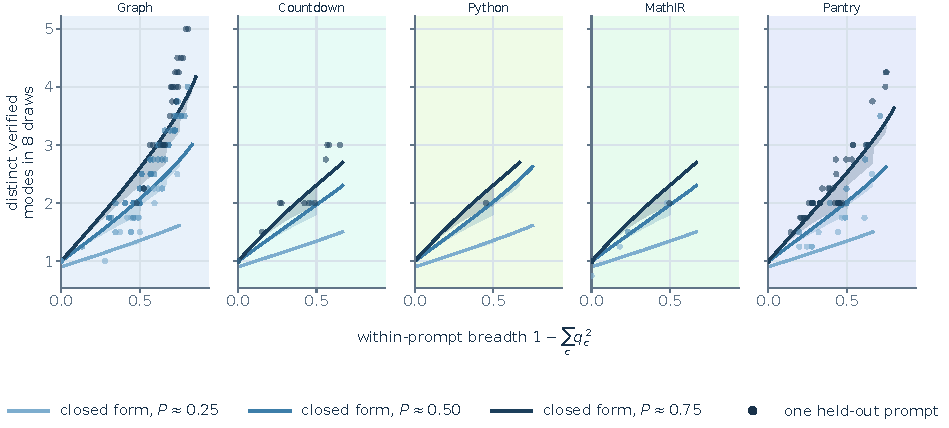
\includegraphics[width=.86\linewidth]{figures/replay_bank_decomposition.pdf}
  \caption{\textbf{Uniform allocation maximizes sampled diversity at fixed buffered probability mass.}
  The horizontal axis traces allocations from a single mode to a uniform
  distribution over $k$ buffered keys. Dashed curves show $1-(1-P)^8$, the
  probability of sampling at least one buffered key when their total mass is
  $P$. Solid curves show the expected number of distinct buffered keys for
  $P\in\{.25,.50,.75\}$; bands span a range of mode counts based on the
  observed prompts and are analytic ranges rather than confidence intervals.
  Points show held-out Level-1 prompts, which have no replay buffer, evaluated
  at the final Re:Dr and
  Re:Max checkpoints of Qwen2.5-0.5B, using one matched seed and grouping
  prompts by their verified response fraction. Their horizontal coordinates
  use empirical key frequencies in $1-\sum_c q_c^2$, rather than the unbiased
  pair estimator. Both coordinates use the same sampled responses, so the
  scatter illustrates agreement with the analytic relationship rather than
  an independent prediction of diversity on new responses.}

  \label{fig:replay-bank-decomposition}
\end{figure}

These properties describe the categorical objective on training-prompt buffers.
Generalization is measured on held-out prompts, whose responses never enter
the buffers. The surrogate alone does not establish that the implemented
response-level objective increases held-out \pmd{}.

% Shared long-paper and workshop benchmark/protocol appendix.

\clearpage
\phantomsection
\begin{center}\large\textbf{Part II. Benchmark and method}\end{center}
\addcontentsline{toc}{part}{Part II. Benchmark and method}

\section{Benchmark and Evaluation Protocol}
\label{app:data}
\label{app:experimental-design}
\label{app:domain-overview}
\label{app:data-inventory}

\mb{} uses a single executable validator to determine correctness and
solution identity, through the map $V(\cdot,s_x)$ defined in
App.~\ref{app:metric-details}. Invalid outputs receive reward zero and no
key; valid outputs receive reward one and a canonical execution key. The
valid-key catalogue and its size are unavailable to the learner and are not
used to schedule replay or determine when training stops.
Table~\ref{tab:tasks} summarizes the five domains and the response variants
that share a key. The datasets are available in the
\href{https://huggingface.co/datasets/od2961/ModeBench}{public release};
the training comparisons in this paper cover Levels 1--3.

\begin{table}[!htbp]
  \centering
  \caption{\textbf{Executable solution identities in the five \mb{} domains.}
  The validator determines both correctness and identity, while the catalogue
  of valid modes is unavailable during training. \emph{Valid modes} reports
  the mean and range of certified catalogue sizes over the Level-1 evaluation
  split. These catalogues need not include every accepted output:
  \texttt{Countdown}, for example, accepts valid keys outside its enumeration.
  \emph{Reached} reports mean distinct verified modes from one hosted
  deployment using 512 draws on 32 prompts
  per domain (Fig.~\ref{fig:gpt56-sampling-budget}). These prompts were
  selected from the evaluation split independently of model outputs. The two
  columns therefore summarize the full split and a subset, respectively.
  \texttt{MathIR}'s catalogue includes longer derivations; limited observed
  coverage does not establish whether these routes are inaccessible or simply
  too rare to observe at the given budget. Higher levels have different
  constructions and mode-count distributions (App.~\ref{app:data-levels}).
  The full prompts and model-specific chat templates appear in App.~\ref{app:prompts}.}

  \label{tab:tasks}
  \scriptsize
  \setlength{\tabcolsep}{5pt}
  \renewcommand{\arraystretch}{1.08}
  \begin{tabularx}{\linewidth}{@{}l
      >{\hsize=1.3\hsize}Y
      >{\hsize=.8\hsize}Y
      >{\hsize=.9\hsize}Y
      rr@{}}
    \toprule
    \textbf{Domain} & \textbf{Generated answer / check} &
    \textbf{Executed key} & \textbf{Equivalent responses} &
    \textbf{Valid modes} & \textbf{Reached} \\
    \midrule
    \texttt{Graph} coloring & Complete assignment; check fixed colors and edges &
    Color vector & Spacing only & 6.27 & 2.53 \\
      & & & & {\scriptsize4--12} & \\
    \addlinespace[2pt]
    \texttt{Countdown} & Parse operands; execute exactly &
    Normalized AST & Commutative order & 4.52 & 3.47 \\
      & & & & {\scriptsize2--8} & \\
    \addlinespace[2pt]
    \texttt{Python} factors & Execute restricted lambda externally &
    Return vector & Programs with the same return vector & 229.44 & 3.75 \\
      & & & & {\scriptsize16--1{,}512} & \\
    \addlinespace[2pt]
    \texttt{MathIR} & Execute bounded action program &
    State trajectory & Programs with the same states & 5.00 & 1.91 \\
      & & & & {\scriptsize5} & \\
    \addlinespace[2pt]
    \texttt{PantryPlan} & Exact ingredient allocation; check all bounds &
    Ingredient support & Quantity and ordering aliases & 18.19 & 6.91 \\
      & & & & {\scriptsize8--40} & \\
    \bottomrule
\end{tabularx}
\end{table}


\subsection{Solution mode definitions and concentration by domain}
\label{app:mode-keying}

\mb{} defines solution modes through three kinds of executable identity.
In \texttt{Countdown} and \texttt{MathIR}, distinct modes are different routes to the same
answer. In \texttt{Python}, they are different return vectors on the public test
inputs. In \texttt{Graph} and \texttt{PantryPlan}, they are different valid answers. The
response budgets also differ (Table~\ref{tab:run-contract}): a \texttt{PantryPlan}
response is a short plan, while a \texttt{Countdown} response is a derivation.
These keys identify verified solutions, not latent reasoning processes.

\paragraph{Sensitivity to the chosen equivalence.}
The canonical key determines which responses count as distinct solutions.
A coarser, task-relevant equivalence can therefore change the measured
diversity gain. App.~\ref{app:coarser-keys} tests one such equivalence per
domain. Most contrasts persist, but the replay gain for Level-3
\texttt{Python} with the original wording falls from $.419$ to zero when
$d$ and $n/d$ are treated as the same unordered factor pair. Among the five
domains, \texttt{Python} is the most sensitive to this choice. Evidence that
the gain extends beyond the original key definitions comes from the other
domains. Training uses the original canonical keys throughout; the coarser
analysis measures sensitivity to alternative definitions of solution identity.

\paragraph{Answer-only training prompts.}
The training prompts request only the final answer
(App.~\ref{app:prompts}), with response budgets chosen accordingly.
Restricting outputs to executable answers allows the validator to determine
solution identity directly, without a learned judge or an embedding-similarity
threshold. The finite solution catalogues also provide the reference values
in Table~\ref{tab:absolute-support-references}. For example, uniform sampling
over the 64 ingredient-selection bit masks in \texttt{PantryPlan} reaches
more verified modes than any trained policy evaluated here.

The training experiments do not measure diversity in long reasoning traces.
The separate hosted-model evaluations include reasoning-enabled deployments
and also exhibit concentration (App.~\ref{app:hosted-mode-diversity}), but
these inference-only observations do not establish how training changes
reasoning behavior.

Across RLVR-only arms, the mean initial-to-terminal increase in conditional
collision is $+0.202$ for route-keyed domains over
98 seed-blocks, $+0.201$ for the behavior-keyed
domain over 15, and $+0.404$ for answer-keyed
domains over 106. All three grouped means increase, with the
largest increase in the answer-keyed group. These comparisons describe
concentration under each definition; differences between domains do not
isolate the effect of choosing a particular key.

\texttt{Countdown}'s mean collision increase is $+0.383$ over
46 seed-blocks, compared with $+0.230$ in \texttt{Graph}.
Thus concentration also occurs among different derivations of a common
answer. \texttt{MathIR} has a smaller increase, $+0.042$. Its certified
catalogue includes longer derivations that are absent from the observed
outputs (App.~\ref{app:algorithm-identity}). Their absence at the evaluated
budgets does not establish that those modes are unreachable.

\paragraph{Explicit-reasoning settings and observed solution counts.}
App.~\ref{app:hosted-reasoning-control} compares five deployments on the
same 480 prompts, with eight responses per prompt and an 8,192-token output
cap in both conditions. Disabling explicit reasoning through the provider
interface lowers overall mean \texttt{distinct@8} in all five deployments:
GPT-5.6 Sol changes from 1.62 to 0.99 and GPT-5.4 from 1.85 to 1.18.
These counts include unsolved prompts and depend on both correctness and
allocation among verified solution modes. Changes in success-conditional
\pmd{} differ across deployments, so lower raw counts do not establish a
common increase in conditional concentration. The requested setting does
not establish the absence of hidden computation, and collection times and
provider defaults can also differ. This comparison therefore describes
solution distributions under the tested configurations, without identifying
an isolated effect of internal deliberation.

\subsection{Dataset splits and validation}
\label{app:data-materialization}

Each domain has disjoint training and evaluation splits
(Table~\ref{tab:run-contract}). \texttt{PantryPlan} and Level 2 also include
separate development splits (App.~\ref{app:data-levels}). For every
\texttt{Python} problem, execution verifies at least two functions with
distinct valid return vectors. For \texttt{MathIR}, each catalogue route is
checked with the same interpreter used to evaluate model outputs.

\begin{table}[!htbp]
\centering
\caption{\textbf{Dataset sizes and certified mode counts.} \texttt{Python} and \texttt{MathIR}
use disjoint training and evaluation splits. Catalogue ranges refer to the
training split; Table~\ref{tab:tasks} gives evaluation-split counts.}

\label{tab:materialization-identities}
\small
\begin{tabular}{@{}lrr@{}}
\toprule
& \textbf{\texttt{Python} factors} & \textbf{\texttt{MathIR} action menu} \\
\midrule
Training problems & 384 & 384 \\
Evaluation problems & 128 & 128 \\
Certified modes per prompt (train) & 16--3{,}600 & 5 \\
\bottomrule
\end{tabular}
\end{table}

\paragraph{\texttt{PantryPlan}.}
\label{app:data-pantry}
\texttt{PantryPlan} contains 384 training, 64 development, and 128 evaluation
prompts across four problem families. The number of feasible ingredient
supports ranges from 8--45 in training and
8--40 in evaluation, with an evaluation mean of
18.19. The validator checks inventory, serving increments, mass,
nutrient bounds, and dietary restrictions using exact arithmetic. The solution
key records which ingredients are used. These checks establish satisfaction
of the stated constraints; they do not assess taste, preparation feasibility,
or food safety.

\subsection{\texttt{Python} execution and validation}
\label{app:python}
\label{app:python-language}

After removing surrounding whitespace, the validator parses each candidate
as a Python expression, with limits of 240 characters and 64 abstract syntax
tree (AST) nodes. The accepted form is \texttt{lambda n: EXPR}, with one
ordinary argument named \texttt{n} and no default value, positional-only,
keyword, or variadic arguments. Integer literals have absolute value at most
10,000. Permitted expressions use \texttt{n}, addition, subtraction,
multiplication, floor division, remainder, integer comparisons, Boolean
\texttt{and}/\texttt{or}, unary plus/minus/\texttt{not}, and conditionals.
The validator rejects Boolean and non-integer literals, calls, imports,
attributes, comprehensions, containers, subscripts, assignment, loops, and
other identifiers.

The task specification contains $J$ distinct integers in $[4,1000]$, with
$2\le J\le8$. Every Level-1 problem uses 4 inputs drawn from
$[6,96]$ and admits at least two valid return vectors.

\paragraph{External execution.}
\label{app:python-process}
Candidate expressions run in an isolated Python process with an empty
\texttt{\_\_builtins\_\_} environment. The process repeats the syntax checks
and evaluates the function on the fixed inputs, subject to a 0.25-second
execution limit and a one-second response deadline. Timeouts, execution errors,
malformed results, non-integer outputs, and failed divisor checks produce
$\bot$ and zero reward. Only a validated integer return vector receives a key.

\paragraph{Behavioral identity.}
\label{app:python-identity}
For each of the $J$ fixed inputs $n_j$, the returned $d_j$ must be an integer
but not a Boolean, satisfy $1<d_j<n_j$, and divide $n_j$ exactly. All checks
must pass. The key is the ordered return vector $(d_1,\ldots,d_J)$;
two programs share a key exactly when these vectors agree. The exact support count
$\prod_j|\{d:1<d<n_j,\ d\mid n_j\}|$ is used only for dataset validation.

\subsection{Matched level constructions}
\label{app:data-levels}

Levels 2--5 expand the search space while preserving the verifier,
canonicalizer, and solution-mode definition. Level 2 is harder for the same
model; Levels 3--5 are calibrated against a fixed Level-1 reference using
larger models, with an exception for Level-4 \texttt{MathIR}.

\paragraph{Level 2.}
Level 2 contains 384 training, 128 development, and 128 evaluation problems,
with no shared problem identities across its splits or with Level 1.
The training distribution of valid-key counts matches that of Level 1.
For \texttt{Graph}, \texttt{Countdown}, \texttt{Python}, and \texttt{MathIR},
the development and evaluation distributions match separate Level-1 reference
sets used for dataset construction. \texttt{PantryPlan} uses its existing
Level-1 splits as references; its 64-prompt development histogram is scaled
by two to define the target counts for the 128-prompt Level-2 development set.

The Level-1 construction reference sets differ from the evaluation sets used
to compare trained policies. Consequently, those evaluation sets have different
valid-key-count distributions across levels in \texttt{Graph},
\texttt{Countdown}, and \texttt{Python}. Cross-level differences reflect both
problem structure and evaluation population, and cannot isolate difficulty
at a fixed distribution of mode counts. Within each level, replay and control
conditions use the same prompts, seeds, fresh-sample objective, and training
budget.

\begin{table}[!htbp]
\centering
\caption{\textbf{Structural differences between Levels 1 and 2.}
The verifier, canonicalizer, and definition of a solution mode are unchanged;
Level 2 expands the search space.}
\label{tab:level2-structure}
\small
\begin{tabularx}{.96\linewidth}{@{}lYY@{}}
\toprule
\textbf{Domain} & \textbf{Level 1} & \textbf{Level 2 structural change} \\
\midrule
\texttt{Graph} coloring & Three hidden vertices & Four hidden vertices \\
\texttt{Countdown} & Three operands & Four operands, with values up to 14 \\
\texttt{Python} factors & Four executed cases, all at most 96 & Four cases, including a value above 96 \\
\texttt{MathIR} & One-sided linear families & Variable-on-both-sides families \\
\texttt{PantryPlan} & Base dietary/composition constraints & More active dietary exclusions and tighter composition \\
\bottomrule
\end{tabularx}
\end{table}

On every domain's development split, fixed Qwen2.5-0.5B has
\texttt{pass@8} in $[.10,.90]$, below its Level-1 construction reference
when both levels use identical decoding settings.

\paragraph{Scale-calibrated Level 3.}
Level 3 is calibrated using Qwen2.5-3B, with Qwen2.5-0.5B on Level 1 as the
reference. Model weights remain fixed. Construction parameters are fitted
on development problems and assessed on held-out prompts. In every domain,
the calibration requires absolute differences from the reference of at most
$.04$ in pass@1 and $.08$ in pass@8, measured using four independent groups
of eight samples per prompt. \distk{} is excluded from the fitting objective.

Both models use their native chat templates, temperature 1, top-$p$ 1, and a
192-token generation limit. \texttt{Graph} prompts request only a boxed final
answer. The other domains receive task-specific solution guidance and use
decoding constrained to legal output syntax, without filtering candidates by
correctness. These criteria establish an empirical match to the reference
success rates rather than a formal two-sided equivalence test.
The Level-3 \texttt{Python} hint ablation removes the strategy guidance
(App.~\ref{app:prompt-hint-ablation}); its difficulty is therefore outside
the scope of this calibration.

\paragraph{Levels 4 and 5.}
Levels 4 and 5 are calibrated with 7B and 14B models, respectively, against
the same Qwen2.5-0.5B Level-1 reference, using pass@1 and pass@8 tolerances
of $.04$ and $.08$.
Level 5 meets these criteria in all five domains. Level 4 meets them in \texttt{Graph},
\texttt{Countdown}, \texttt{Python}, and \texttt{PantryPlan}, but not \texttt{MathIR}.

For \texttt{MathIR}, the reference pass@8/pass@1 ratio is $5.50$, whereas
the largest ratio among the evaluated 7B constructions is $4.16$. A ratio
of mixture means cannot exceed the largest component ratio, so mixing these
constructions cannot reproduce the reference ratio exactly.

The heterogeneity gap, $1-(1-\bar P)^8-\overline{\texttt{pass@8}}$, compares
observed pass@8 with its value if every prompt had the same correctness
$\bar P$. The measured gaps are $.169$--$.398$ at 7B and $.060$ for the
reference. Because the gap depends on mean correctness $\bar P$, these values
are not directly comparable across correctness levels. Each Level-4 domain
contains 384 training, 128 development, and 128 evaluation prompts, disjoint
from other levels. Level-4 \texttt{MathIR} appears in
Figs.~\ref{fig:base-levels-all-scales} and~\ref{fig:level-construction}
but is not difficulty-matched to the reference.

\subsection{Model performance across all five levels}
\label{app:base-levels-all-scales}

Fig.~\ref{fig:base-levels-all-scales} compares Qwen2.5-Instruct across five
levels and domains; Fig.~\ref{fig:families-appendix} adds three model families,
for 375 model--domain--level measurements before benchmark training.
Each measurement uses the same 128 held-out prompts per domain and level,
with four independent groups of eight responses per prompt, totaling 4,096
responses. For \texttt{pass@8} and \distk{}, we score each group, average
within prompts, and then average prompts. For \pmd{}, we pool the four
groups within each prompt (App.~\ref{app:metric-sampling}).

Evaluation uses native chat templates, temperature 1, top-$p=1$, and a
192-token output limit. \texttt{Graph} prompts request boxed final answers;
other domains use task-specific solution guidance and syntax-constrained
decoding. These settings differ from the training evaluations: under the
training template and its larger sample, the same untrained Level-1
\texttt{Python} model defines \pmd{} on 73 of 128 prompts, with mean $.168$
(Section~\ref{sec:results-collapse}). Training effects are therefore measured
against the untrained model under the corresponding evaluation conditions.

Success does not necessarily decrease monotonically with level.
\texttt{pass@8} at the highest evaluated level is below its Level-1 value in
33 of 35 model--domain series. Model scale and
benchmark level also affect diversity differently: the median range of
\pmd{} across scales at a fixed level is .251, compared with
.104 across levels at a fixed scale.

\begin{figure}[!htbp]
  \centering
  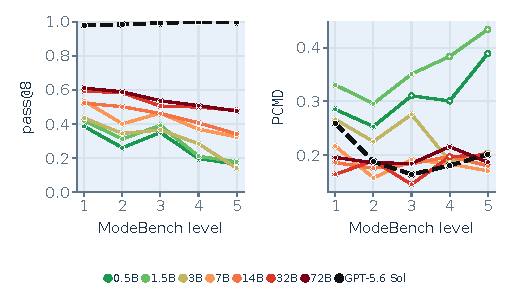
\includegraphics[width=.62\linewidth]{figures/qwen_level_trends.pdf}
  \caption{\textbf{Accuracy and solution diversity vary differently across benchmark levels.}
  Left: \texttt{pass@8}; right: \pmd{}, averaged with equal domain weights
  for each Qwen2.5-Instruct scale (colored lines) and GPT-5.6 Sol (black dashed
  line). This Qwen evaluation augments the 128 held-out prompts with the 384
  training-split prompts where available; none were used to train these
  checkpoints. Filled diversity markers indicate at least 30 prompts with
  two or more correct responses in every domain. Hollow markers average the
  available estimates when at least one domain has insufficient support;
  the set of contributing domains can differ when an estimate is undefined.}

  \label{fig:qwen-level-trends}
\end{figure}

\begin{figure}[!htbp]
  \centering
  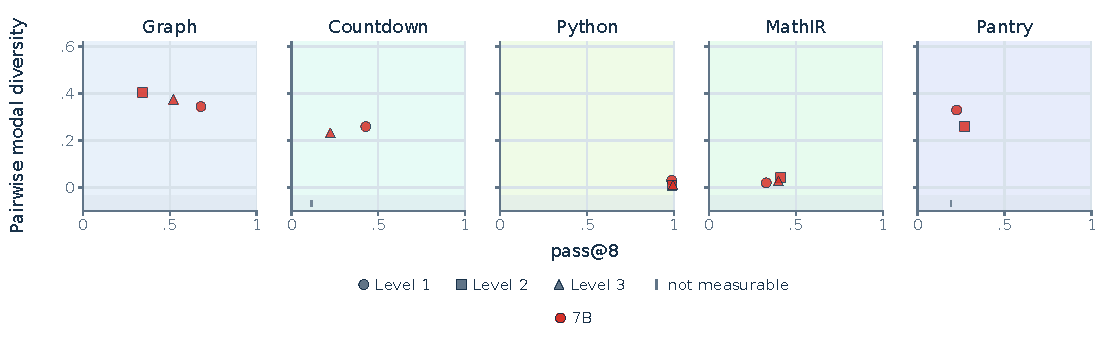
\includegraphics[width=\linewidth]{figures/mode_diversity_level_construction.pdf}
  \caption{\textbf{High accuracy can coexist with low solution diversity.}
  Each row shows one checkpoint before benchmark training, with domains in
  columns, \texttt{pass@8} on the horizontal axis, and \pmd{} on the vertical
  axis. Color indicates parameter count and marker shape indicates level.
  Each measurement uses four groups of eight responses to 128 held-out
  prompts at temperature 1; \pmd{} pools the groups within each prompt.
  Filled markers indicate at least 30 prompts with two or more correct
  responses. Hollow markers indicate 5--29 such prompts and show one standard
  error. Ticks below the axis mark measurements with fewer than five eligible prompts.}

  \label{fig:level-construction}
\end{figure}

\begin{figure}[!htbp]
  \centering
  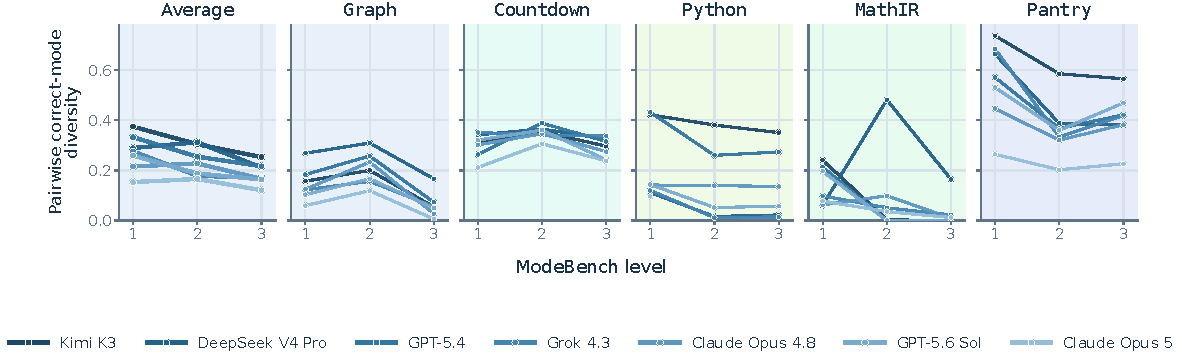
\includegraphics[width=\linewidth]{figures/frontier_level_grid.pdf}
  \caption{\textbf{Mean solution diversity is lower at Level 3 than at Level 1 for every evaluated hosted deployment.}
  Lines show \pmd{} for 7 deployments, with eight
  responses to each of 128 held-out prompts per domain and level. Panels show
  individual domains and their equally weighted mean. For each deployment,
  the set of domains contributing to the mean is fixed across levels.
  Darker lines indicate higher overall diversity. Hollow markers fall below
  the 30-prompt support threshold and are excluded from connecting lines.
  Higher levels change problem structure and add strategy guidance in
  \texttt{MathIR}, \texttt{Python}, and \texttt{PantryPlan}
  (App.~\ref{app:prompt-hint-ablation}); these curves reflect both changes.}

  \label{fig:frontier-level-grid}
\end{figure}

\begin{figure}[!htbp]
  \centering
  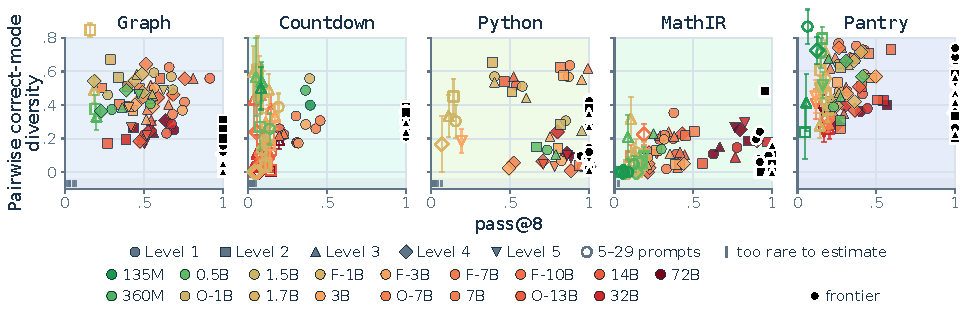
\includegraphics[width=.92\linewidth]{figures/mode_diversity_families_appendix.pdf}
  \caption{\textbf{Models of similar size can differ in solution diversity.}
  SmolLM2, Qwen2.5, Falcon3, and OLMo-2 checkpoints are compared by
  \texttt{pass@8} and \pmd{} across five domains and the available levels,
  before benchmark training. Color indicates parameter count on a logarithmic
  scale; marker shape indicates level. Black markers show the
  7 hosted deployments. Local models use four groups
  of eight responses to 128 held-out prompts per domain and level; hosted
  deployments use eight responses per prompt. Filled markers indicate at
  least 30 prompts with two or more correct responses. Hollow markers
  indicate 5--29 and show one standard error. Ticks below the axis indicate
  fewer than five eligible prompts, for which no diversity estimate is reported.}

  \label{fig:families-appendix}
\end{figure}


\FloatBarrier
\subsection{Other model families at matched scale}
\label{sec:families-appendix}

Fig.~\ref{fig:families-appendix} compares SmolLM2, Qwen2.5, Falcon3, and
OLMo-2 on the same 128 held-out prompts per domain and level. All use four
groups of eight responses, the same verifier, and the same eligibility
thresholds. Comparisons across families use the 4 shared
levels; only Qwen2.5 is evaluated at Level 5. Color denotes parameter count.

Families differ in diversity even at similar parameter counts. Near 7B,
Qwen2.5, Falcon3, and OLMo-2 have different \pmd{} values despite similar
\texttt{pass@8}. Their ordering persists in the 10--15B range, where Falcon3
and OLMo-2 are close. Within parameter-count bands, the median range of
\pmd{} across family means is .166, compared with
.198 across scales within a family, over the
4 shared levels. The earlier .251 summary instead
compares all seven Qwen scales at each level. These descriptive comparisons
do not isolate which pretraining or post-training choices account for the
differences between models.

\clearpage
\subsection{Training and evaluation settings}
\label{app:repro-run-contract}
\label{app:comparison-design}

% [H] pinned this table to the head of the subsection, and being too tall for
% what the previous page had left it took a page of its own and stranded the
% remainder. Floating lets the prose that follows it close the gap.
\begin{table}[!htbp]
  \centering
  \caption{\textbf{Paired comparisons use the same numbers of optimizer updates and fresh rollouts.}
  Treatment and control share the settings below. Both compute replay scores
  and execute the backward pass, but the replay gradient is exactly zero in
  the control. Their buffer contents can differ, so replay workloads, total
  floating-point operations, and wall-clock time are not matched. The control
  receives no additional training in place of replay computation
  (App.~\ref{app:compute-matching}).}

  \label{tab:run-contract}
  \small
  \begin{tabularx}{\linewidth}{@{}P{.23\linewidth}Y@{}}
    \toprule
    \textbf{Component} & \textbf{Setting} \\
    \midrule
    Data & 384 training and 128 disjoint evaluation prompts per domain and
      level; evaluation prompts are excluded from training and replay. \\
    Fresh rollouts & $G=16$, temperature 1, top-$p=1$; one prompt group per update. \\
    Optimization & Eight training passes (3,072 updates), with one PPO epoch
      per batch. $\beta_{\mathrm{KL}}=0$ except in the reference-KL comparison
      (App.~\ref{app:kl-measured}), which varies only this coefficient.
      Paired conditions share initialization, prompt order, optimizer,
      hardware class, and checkpoint frequency. \\
    Evaluation & At passes $0,.5,\ldots,8$: four groups of eight responses
      per prompt at temperature 1 and top-$p=1$, plus a separate greedy
      response at temperature 0. Final comparisons use the last checkpoint. \\
    Replay & Capacity $M=16$ keys per prompt; buffers are selected in
      round-robin order, one per update; $\lambda_{\mathrm{replay}}=.10$.
      The control has zero replay gradient; buffer contents and computational
      workloads may differ between conditions. \\
    Training seeds & Five per model--domain combination; paired comparisons use
      common seeds, with sample sizes reported alongside the results. \\
    Learning rate & Qwen2.5-0.5B and Falcon3-1B: constant $2\times10^{-7}$,
      with Falcon optimizer states stored on the CPU. Qwen2.5-3B: cosine
      decay from a $10^{-7}$ peak to a $10^{-8}$ floor, with 10\% warmup. \\
    Optimizer & Fused Adam in \texttt{bf16} with decoupled weight decay,
      $\beta_1=.9$, $\beta_2=.95$, weight decay $0$, gradient-norm clip $1.0$,
      with gradient checkpointing. CPU offloading uses the corresponding
      CPU optimizer implementation with the same hyperparameters. \\
    Policy update & Parameters are synchronized after every update, and each
      rollout is used once in a single PPO epoch. The symmetric clipping
      threshold is $\varepsilon=.2$. The importance ratio equals $1$ when
      the surrogate is evaluated in this update scheme, so clipping is inactive. \\
    % All twelve cells are the OAT_ZERO_GENERATE_MAX_LENGTH actually submitted,
    % read per domain from the job ledgers rather than from a launcher default:
    %   0.5B  var/artifacts/e72_frontier_source_runs.json
    %           (inherited_eval_config.generate_max_length; the 3B cohort
    %            inherits this record and overrides only the base model)
    %   1B    var/artifacts/e79_falcon1b_aligned_verified_replay_jobs.json
    %   3B    var/artifacts/e80r1_qwen3b_aligned_verified_replay_jobs.json
    % ops/train.sh defaults this to 192, so a domain that is 192 looks the same
    % whether it was chosen or inherited; the ledgers are what distinguish them.
    Response tokens & \texttt{Graph} and \texttt{Countdown}: 192; \texttt{Python}: 192/512/192
      at 0.5B/1B/3B; \texttt{MathIR}: 64/128/64; \texttt{PantryPlan}: 8. \\
    \bottomrule
  \end{tabularx}
\end{table}



For each training seed, \texttt{pass@8} and \texttt{distinct@8} are averaged
over four eight-response groups per prompt and all 128 evaluation prompts;
\texttt{mean@8} is the fraction of correct responses. Responses are independent
within a group. Independence across groups, required for the pooled \pmd{}
interpretation, depends on the sampling procedure described in
App.~\ref{app:metric-sampling}. Evaluation outputs are excluded from training
and replay, and do not determine checkpoint selection or stopping.

Comparisons use paired final checkpoints. Comparisons with five matched
training seeds use nominal pointwise 95\% Student-$t$ intervals; other main
checkpoint comparisons report sample sizes and descriptive means. Diversity
comparisons use the prompt-eligibility thresholds and interval procedures
specified alongside their results. Intervals condition on the fixed evaluation
prompts and sampled responses. The replay-weighting comparison instead uses
a bootstrap over paired training seeds.

% Finish benchmark floats before beginning the prompt examples.
\FloatBarrier
\section{Exact Domain Prompts}
\label{app:prompts}

Each domain's training prompt contains one system message and one user
message, without few-shot examples. Training and evaluation use the same
template within each method. The examples below reproduce the first prompt
from each Level-1 evaluation split in Qwen's chat format. Falcon3 uses the
same message text with its own \texttt{<|system|>} and \texttt{<|user|>}
markers. Models evaluated before benchmark training use their tokenizer's
native chat template (App.~\ref{app:base-levels-all-scales}).
App.~\ref{app:data-levels} describes the different problems and prompting
conditions at Levels 2--5.

The examples preserve the prompt text. A continuation line indented by two
spaces indicates a display line break; replacing that break and indentation
with one space recovers the original text. In the \texttt{PantryPlan}
example, a line break without this indentation is part of the prompt.

% BEGIN generated by ops/check_paper_domain_prompts.py

\filbreak
\subsection{\texttt{Graph} coloring}
\label{app:prompt-graph}

\noindent 384 training and 128 evaluation prompts.

\begin{Verbatim}[fontsize=\scriptsize,frame=single,framesep=4pt,rulecolor=\color{black!25},samepage=true]
<|im_start|>system
Return only the final answer inside \boxed{}. Do not explain.<|im_end|>
<|im_start|>user
Color this graph with vertices 1 through 6. The undirected edges are: (1,2), (1,3),
  (3,5), (3,6), (4,6), (5,6). Assign each vertex one color from {1, 2, 3} so that no
  edge has the same color on both endpoints. A partial coloring is 2??1?2, where ?
  means uncolored. Keep every shown digit fixed. There are exactly 3 question marks.
  Return exactly one final answer and no explanation: exactly 3 digits, each one 1,
  2, or 3, for the missing positions from left to right, inside \boxed{}.<|im_end|>
<|im_start|>assistant
\end{Verbatim}

\filbreak
\subsection{\texttt{Countdown}}
\label{app:prompt-countdown}

\noindent 384 training and 128 evaluation prompts.

\begin{Verbatim}[fontsize=\scriptsize,frame=single,framesep=4pt,rulecolor=\color{black!25},samepage=true]
<|im_start|>system
Return only the final answer inside \boxed{}. Do not explain.<|im_end|>
<|im_start|>user
Using the numbers [3, 6, 9], create an arithmetic expression that equals 18. Use
  each given number exactly once. You may use +, -, *, /, and parentheses. Return
  exactly one final answer and no explanation: the expression inside
  \boxed{}.<|im_end|>
<|im_start|>assistant
\end{Verbatim}

\filbreak
\subsection{\texttt{Python} factors}
\label{app:prompt-python}

\noindent 384 training and 128 evaluation prompts.

\begin{Verbatim}[fontsize=\scriptsize,frame=single,framesep=4pt,rulecolor=\color{black!25},samepage=true]
<|im_start|>system
Return only the final answer inside \boxed{}. Do not explain.<|im_end|>
<|im_start|>user
Write one pure Python function with the exact form lambda n: EXPR. An external
  Python tool will call it once for each n in [18, 82, 91, 93]. For every call,
  return an integer d satisfying 1 < d < n and n % d == 0. Different valid return
  vectors are different solution modes. You may use integer literals, n, +, -, *,
  //, %, comparisons, Boolean operators, and conditional expressions; calls,
  imports, attributes, containers, and other names are forbidden. Return exactly the
  one-line lambda inside \boxed{} and no explanation.<|im_end|>
<|im_start|>assistant
\end{Verbatim}

\filbreak
\subsection{\texttt{MathIR} action menu}
\label{app:prompt-mathir}

\noindent 384 training and 128 evaluation prompts.

\begin{Verbatim}[fontsize=\scriptsize,frame=single,framesep=4pt,rulecolor=\color{black!25},samepage=true]
<|im_start|>system
Return only the final answer inside \boxed{}. Do not explain.<|im_end|>
<|im_start|>user
MathIR linear-menu-v1. Solve for x by choosing an executable action sequence. Every
  selected action is applied exactly to BOTH sides of the current equation, followed
  by exact simplification. Bindings: a=2, b=-9, c=-1. Initial equation: x/a + b = c.
  Action menu: A means div(a); B means add(b); C means sub(b); D means sub(c); E
  means sub(mul(a,b)); F means mul(a). Choose 1-4 action IDs. Illegal operations,
  repeated states, and paths that do not finish with x isolated are rejected. Return
  only the IDs separated by semicolons inside the answer box; for example formatting
  only: \boxed{A;C}. Do not return x's numeric value.<|im_end|>
<|im_start|>assistant
\end{Verbatim}

\subsection{\texttt{PantryPlan}}
\label{app:prompt-pantry}

\noindent 384 training and 128 evaluation prompts.

\begin{Verbatim}[fontsize=\scriptsize,frame=single,framesep=4pt,rulecolor=\color{black!25},samepage=false]
<|im_start|>system
Return only six binary digits and no other text. Each digit maps to the
  corresponding Pantry row in printed order. A trusted environment will choose exact
  quantities on precisely the selected rows.<|im_end|>
<|im_start|>user
Create one feasible high fiber snack from this frozen pantry.
Nutrition values are per 100 g. Quantities are exact integer grams.

Pantry:
- almonds: available=100g, step=25g, minimum-if-used=50g; energy=584kcal,
  protein=21.5g, fiber=10.8g, sodium=0.0mg; tags=tree_nut
- banana: available=125g, step=25g, minimum-if-used=50g; energy=97.0kcal,
  protein=0.74g, fiber=4.62g, sodium=0.0mg; tags=none
- carrots: available=150g, step=25g, minimum-if-used=50g; energy=45.0kcal,
  protein=0.941g, fiber=3.1g, sodium=86.6mg; tags=none
- grape_tomatoes: available=100g, step=25g, minimum-if-used=50g; energy=27.0kcal,
  protein=0.83g, fiber=2.1g, sodium=6.0mg; tags=none
- navel_orange: available=150g, step=25g, minimum-if-used=50g; energy=47.0kcal,
  protein=0.91g, fiber=2.0g, sodium=9.0mg; tags=none
- sunflower_seeds: available=125g, step=25g, minimum-if-used=50g; energy=571kcal,
  protein=18.9g, fiber=7.22g, sodium=0.0mg; tags=none

Use 2 to 4 ingredients.
Forbidden tags: none
Targets:
- mass_g: minimum 125, maximum 200
- energy_kcal: minimum 239.4, maximum 432.25
- protein_g: minimum 6.423
- fiber_g: minimum 3.478
- sodium_mg: maximum 37.6

Choose the ingredient support as a six-bit mask in the exact Pantry row order. Bit 1
  includes that row and bit 0 excludes it.<|im_end|>
<|im_start|>assistant
\end{Verbatim}

% END generated by ops/check_paper_domain_prompts.py

% Shared exact replay update; empirical comparisons are in results.tex.

\section{Replay Algorithm}
\label{app:algorithm}

Verified replay combines learning from newly sampled responses with a
likelihood loss on stored, verified solutions. Each prompt $x$ has a buffer
$\mathcal B_x$ of at most $M$ exemplars, with one response per canonical key.
A round-robin cursor $\sigma$ selects one prompt's buffer at each update,
and all keys in that buffer contribute equally to the replay loss.
Table~\ref{tab:notation} defines the notation;
App.~\ref{app:replay-metric-alignment} relates this objective to diversity.

\subsection{Fresh task advantages}
\label{app:binary-maxrl}

For a group of $G$ fresh responses with verified binary rewards $R_i$ and
$R=\sum_i R_i$, Dr.GRPO uses $A_i=R_i-R/G$, while MaxRL uses
\[
 A_i^{\mathrm{MaxRL}}=
 \begin{cases}
 G R_i/R-1, & R>0,\\
 0, & R=0.
 \end{cases}
\]
The centered MaxRL estimator \citep{tajwar2026maxrl} assigns advantage $-1$
to failures in mixed groups and gives each success greater weight when
successes are scarce. Both objectives assign zero task advantage to every
response in an all-correct or all-failure group. Lemma~\ref{lem:maxrl-mean}
derives MaxRL's mean objective as a harmonic combination of pass@\(k\)
terms. These advantages apply to fresh responses; stored exemplars contribute
through the separate replay loss.

\subsection{Optimizer update}
\label{app:algorithm-update}

\begin{algorithm}[H]
  \caption{\textbf{Verified replay update.} The fresh objective selects Re:Dr or Re:Max.}
  \label{alg:verified-replay-update}
  \small
  \begin{algorithmic}[1]
    \REQUIRE Policy $\pi_\theta$; prompt $x$ and verifier specification
      $s_x$; group size $G$; fresh objective
      $o\in\{\mathrm{MaxRL},\mathrm{Dr.GRPO}\}$; replay weight
      $\lambda_{\mathrm{replay}}$; buffer capacity $M$; buffers and cursor
      $(\mathcal B,\sigma)$
    \ENSURE Updated $(\theta',\mathcal B',\sigma')$
    \STATE Draw the on-policy group
      $\mathcal G=\{y_i\sim\pi_\theta(\cdot\mid x)\}_{i=1}^G$
    \FOR{$i=1,\ldots,G$}
      \STATE Execute $\widetilde c_i\gets V(y_i,s_x)$ and observe task
        reward $R_i$
      \STATE Set $c_i\gets\widetilde c_i$ iff
        $R_i>0\wedge\widetilde c_i\ne\bot$; otherwise set $c_i\gets\bot$
    \ENDFOR
    \STATE Compute fresh task advantages $A_i^{o}$ from $\{R_j\}_{j=1}^G$;
      for $o=\mathrm{MaxRL}$ use the formula in App.~\ref{app:binary-maxrl}
    \STATE After the full group is validated, deterministically retain one
      policy exemplar for each new $c_i\ne\bot$ in $\mathcal B_x$, up to
      capacity $M$
    \STATE $(z,\sigma')\gets\textsc{NextBuffer}
      (\{\mathcal B_u\}_u,\sigma)$ by a fixed round-robin cursor over
      prompts; the replayed prompt $z$ need not be the prompt $x$ that
      supplied the fresh group
    \IF{a replay buffer $\mathcal B_z$ exists}
      \STATE For each exemplar $e_c\in\mathcal B_z$, compute
        $\ell_c=|e_c|^{-1}\log\pi_\theta(e_c\mid z)$
      \STATE $L_{\mathrm{replay}}\gets-|\mathcal B_z|^{-1}
        \sum_{c\in\mathcal B_z}\ell_c$
    \ELSE
      \STATE $L_{\mathrm{replay}}\gets0$
    \ENDIF
    \STATE Set the replay-loss normalization $w_{\mathrm{rep}}\gets(G-1)/G^2$
    \STATE $\theta'\gets\textsc{Update}
      (\theta,L_{\mathrm{PPO}}(A^{o})
      +w_{\mathrm{rep}}\lambda_{\mathrm{replay}}L_{\mathrm{replay}})$
\end{algorithmic}
\end{algorithm}

\subsection{Buffer construction and scheduling}
\label{app:algorithm-bank}

Each buffer is associated with an exact prompt-token sequence. A response
is eligible for storage if it has positive task reward and a valid canonical
key, including responses that reach the generation limit. The entire group
is validated before the buffer is updated. For each newly observed key, we
retain the lexicographically smallest normalized response-token sequence;
new keys are inserted in sorted order. Selection therefore does not depend
on the order of responses within the group. Each buffer holds at most
$M=16$ exemplars, one per key, with no eviction or replacement. Keys first
observed after the buffer is full receive no replay support.

At each update, a deterministic round-robin schedule selects one nonempty
buffer, including buffers containing a single exemplar. The choice does not
use reward magnitudes, evaluation results, a target mode count, or entropy.
The policy scores every stored response in the selected buffer by teacher
forcing, conditioned on its original prompt. Each exemplar contributes its
mean response-token log probability, excluding prompt and padding tokens.

The replay loss is the negative mean score over the selected keys,
weighted by $\lambda_{\mathrm{replay}}(G-1)/G^2$
(Algorithm~\ref{alg:verified-replay-update}). The normalization $(G-1)/G^2$
matches the weight of a single success in a centered Dr.GRPO group: its
advantage is $(G-1)/G$, followed by averaging over $G$ responses
(Lemma~\ref{lem:grpo-mean}). This loss uses only discovered training
exemplars; it requires neither the complete valid-key catalogue nor
evaluation outputs.

\subsection{Control without replay gradients}
\label{app:algorithm-control}

Replay and control use the same validation, buffer construction, scheduling,
and exemplar-scoring procedures. The control sets the replay gradient to
zero while retaining the forward and backward computations. Both conditions
combine the fresh-task and replay gradients in one optimizer step; the
replay gradient is their only difference in the learning objective.

As the policies diverge, they can generate different responses and accumulate
different buffers, which changes the selected exemplars and their lengths.
The conditions match optimizer updates and fresh-rollout budgets, but not
realized floating-point operations or wall-clock time. The control receives
no additional task-gradient updates, fresh rollouts, or training time in
place of replay computation. The comparison isolates the contribution of the
replay learning signal under this design, without establishing an advantage
at equal total compute (App.~\ref{app:compute-matching}).

\subsection{Verifier requirements and applicability}
\label{app:algorithm-identity}

Replay requires a deterministic rule for grouping verified responses into
solution modes. Its canonical key must be computable for every training
response at reasonable cost and must reflect the task's definition of a
solution. In \mb{}, one executable validator determines both correctness
and identity, so buffer construction requires no learned judge or
embedding-similarity threshold.

Final-answer grading, as used for MATH, GSM8K, and AIME, does not distinguish
derivations of the same answer. When a prompt has only one correct answer,
an answer-based key places every successful response in the same mode. The
buffer then holds one exemplar, and replay reinforces it without balancing
alternative derivations. That buffer is the capacity-one arm of
App.~\ref{app:mode-agnostic-replay}, which retains 58\% of the
Re:Dr diversity effect and a correctness gain of +.263 against
Re:Dr's +.352. Measuring and replaying distinct derivations
requires a finer definition of identity.

\texttt{MathIR} uses executed state trajectories as keys. Its catalogue
includes verified four-state routes, but none appears among 27,450
verified draws. Across 115 solved Level-1 prompts, these
draws cover 67\% of the certified two-state modes and
52\% of the three-state modes. Different modes rarely appear
for the same prompt. Terminal \pmd{} averages .006, corresponding
to 1.01 effective verified modes per prompt. These results provide
limited evidence for diversity gains among alternative derivations.

Across the 6 comparisons, including \texttt{MathIR} in the
five-domain mean reduces the \pmd{} gain by .010--.074
relative to the corresponding four-domain mean. At Qwen2.5-0.5B, the Re:Dr
gain is +.294 across all five domains and +.364 across the other
four. App.~\ref{app:hosted-mode-diversity} reports hosted-model results for
the same four-domain subset.

For open-ended derivations, a learned judge could supply a novelty criterion,
but that criterion would require independent validation. Judge decisions can
be inconsistent or disagree with task correctness, and replay may reinforce
distinctions that the judge rewards without improving solution diversity.
Fixing the judge model, prompt, and decoding rule does not by itself ensure
a valid equivalence relation. Where executable keys are available, they can
be used to assess the judge and measure diversity separately from its training
signal. We do not evaluate judge-based replay here.

\subsection{Exemplar quality and length}
\label{app:algorithm-quality}

Canonical verification establishes that a response satisfies the task
constraints. It does not validate every intermediate reasoning step: a
verified response may be verbose or include an unsound explanation. Replay
weights exemplars by solution key without ranking their reasoning quality.

Each key occupies one buffer entry and contributes its exemplar's mean
response-token log probability,
$\ell_c=|e_c|^{-1}\log\pi_\theta(e_c\mid z)$. Longer responses therefore do
not receive more buffer entries or loss weight proportional to their token
count. This normalization still affects the learning target. In a categorical
surrogate with one exemplar of fixed length $L_b$ per key, the effective
weights are proportional to $L_b^{-1}$. With full coverage, the limiting
distribution favors shorter exemplars and is uniform only when lengths are
equal (App.~\ref{app:theory-replay}). This conclusion concerns the surrogate;
mean-token normalization does not imply uniform key probabilities in a
language model or guarantee concise, sound explanations.

Additional length or reasoning-quality filters would change which exemplars
enter or remain in the buffer, and hence change the replay target. We use no
such filters beyond the stated generation limits and verification rules.
Restricting length can exclude valid alternatives: \texttt{MathIR} includes
longer state trajectories, and the observed lambdas for rarer \texttt{Python}
return vectors are longer than those for the modal vector. Evaluating a
quality filter would therefore require measuring both solution quality and
diversity among retained modes.

\section{Fixed Semantic-MaxEnt Comparator}
\label{app:semantic-maxent}

Fixed Semantic-MaxEnt adds a frequency-based bonus to the fresh-response
advantage. It counts previously observed verified keys but does not optimize
the likelihood of stored exemplars. For response $i$ in a group of $G$
responses to prompt $x$, let $n_x(a)$ count earlier successful responses
with key $a$, and let $m_{-i}(a)$ count successful responses with that key
among the other members of the current group. Write
$N_x=\sum_a n_x(a)$, $S_{-i}=\sum_a m_{-i}(a)\le G-1$, and let
$\mathcal K_i$ contain all keys observed in these two sources. Adding one
pseudocount per observed key and reserving one for unseen keys gives,
for $a\in\mathcal K_i$,

\begin{equation}
  \hat p_i(a)=\frac{n_x(a)+m_{-i}(a)+1}{N_x+S_{-i}+|\mathcal K_i|+1},\qquad
  \hat p_i(\textsc{unseen})=\frac{1}{N_x+S_{-i}+|\mathcal K_i|+1}.
  \label{eq:open-set-predictor}
\end{equation}
A response whose key is outside $\mathcal K_i$ receives the probability
assigned to the unseen category. Invalid and unsuccessful responses do not
contribute to the counts.

\paragraph{Counts and advantage calculation.}
Counts are specific to each exact prompt-token sequence and accumulate
throughout training without decay or reset. Only responses with positive
reward and a valid key are counted. Each response is scored using previous
groups and the other successful responses in its current group. Counts for
the full current group are added only after scoring, so a response never
contributes to its own predicted probability.
The added advantage for an eligible successful response is held constant
during differentiation and equals

\begin{equation}
  A^{\rm sem}_{i,t}=\eta\,
  \frac{\min\{-\log\hat p_i(a_i),\kappa\}
    -\E_{\hat p_i}[\min\{-\log\hat p_i(a),\kappa\}]}{\kappa},
  \qquad \eta=.10,\ \kappa=5.
  \label{eq:legacy-semantic-advantage}
\end{equation}
The same $A^{\rm sem}_{i,t}$ applies at every token position $t$ of response
$i$. Invalid and unsuccessful responses receive zero bonus. The fixed scale
$\eta$ bounds the centered bonus in magnitude, while $\kappa$ clips the
surprisal. The bonus can favor an underrepresented verified mode when that
mode appears in a fresh response, but it adds no direct likelihood term for
a stored exemplar absent from the group. If neither previous groups nor the other
successful responses provide a key, the unseen category has probability one
and the bonus is zero. App.~\ref{app:ucpo-progress} reports the comparison.

\paragraph{Relation to conditional entropy.}

For the true conditional distribution $q_\theta=p_\theta(\cdot\mid\mathcal C)$,
\begin{equation}
 \nabla_\theta H(q_\theta)
 =\E_{a\sim q_\theta}[(-\log q_\theta(a))\nabla_\theta\log q_\theta(a)].
 \label{eq:entropy-score-function}
\end{equation}
The frequency predictor generally does not provide an unbiased estimator
of this gradient. To see the distinction, hold a predictor score vector $s$
and baseline $b$ fixed independently of the scored action, for example by
conditioning on the other responses in its group. Averaging the gradients
of successful responses under the unconditional policy gives

\[
 \E_{Z\sim p}[\1\{Z\in\mathcal C\}(s_Z-b)\nabla_\theta\log p_Z]
 =P\E_{c\sim q}[s_c\nabla_\theta\log q_c]
   +(\E_q[s]-b)\nabla_\theta P.
\]
The predictor's baseline need not equal the current conditional mean
$\E_q[s]$. The second term can therefore change correctness as well as the
allocation among correct modes. Even with the exact, unclipped score
$s_c=-\log q_c$ and baseline $b=H(q)$, averaging over all rollout responses
yields $P\nabla_\theta H(q)$, scaled by the probability of success.

The distinction also matters when only one correct key exists. Its
conditional entropy is zero, yet probability assigned to the unseen
category can make its semantic advantage negative after it has been
observed. The bonus is therefore generally not an exact conditional-entropy
gradient, and it provides no guarantee of individual-mode preservation.

% Every part divider opens a fresh page, this one included. It used to run on
% from the comparator section to save the white space below that section's end;
% uniformity across the seven dividers is worth the part page.
\clearpage
\phantomsection
\begin{center}\large\textbf{Part III. Training results}\end{center}
\addcontentsline{toc}{part}{Part III. Training results}

\section{Empirical Results and Comparisons}
\label{app:supporting}

\begin{figure}[!htbp]
\centering
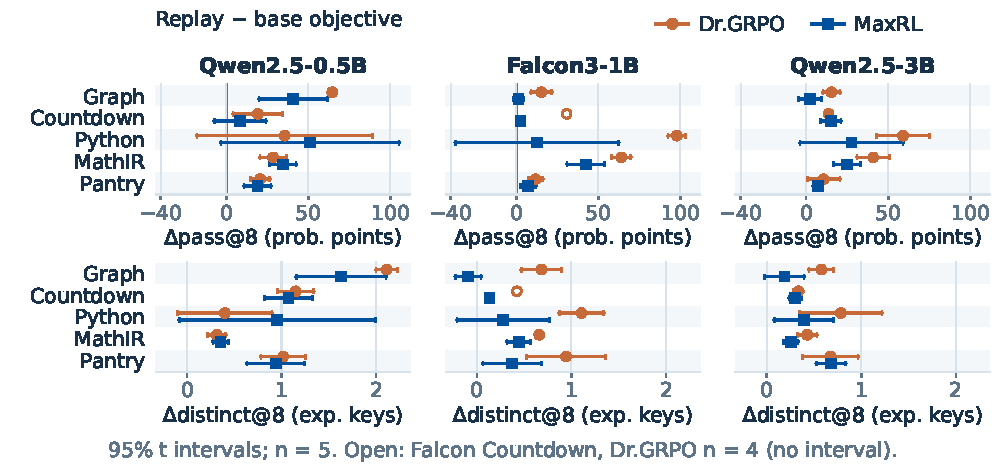
\includegraphics[width=\linewidth]{figures/replay_factorial_effects.pdf}
\caption{\textbf{Replay raises mean correctness at all three model scales.}
Final-checkpoint differences: Re:Dr minus Dr.GRPO (circles) and Re:Max minus
MaxRL (squares), measured in percentage points for \texttt{pass@8} and in
\pmd{} units for diversity. Filled markers use five paired seeds; hollow
markers use fewer. For Re:Dr, correctness uses four seeds in Falcon
\texttt{Countdown}; diversity uses four in Falcon \texttt{Countdown}, one
in Falcon \texttt{MathIR}, and two in Qwen2.5-3B \texttt{Python}. Diversity
requires at least 20 eligible prompts per arm; blanks indicate no eligible
comparison. Bars show nominal paired 95\% Student-$t$ intervals, requiring
five seeds for correctness and at least two for diversity.}
  \label{fig:replay-factorial-effects}
\end{figure}

\subsection{Terminal comparisons across scales}
\label{app:scale-matrix}
\label{app:scale-snapshot}
\label{app:maxrl-scale-extensions}
\label{app:current-campaign-results}

Paired conditions share initialization, training and evaluation prompts,
eight training passes, evaluation requests, the verifier, and replay schedule.
The control uses the same buffer construction and scoring procedures with
zero replay gradient. Policies can develop different buffers and workloads,
so total compute is not matched (App.~\ref{app:compute-matching}).

\crossscaletablematerial

\paragraph{Dr.GRPO retention contrasts.}
\label{app:retention-numerical-detail}

% Floats rather than [H] so it can rise to the page its discussion starts
% on instead of forcing a break and leaving the preceding page part empty.
\begin{table}[!tbp]
  \centering
  \caption{\textbf{Replay improves mean correctness and solution diversity at each tested scale.}
  Final-checkpoint differences between Re:Dr and Dr.GRPO, by domain and
  model. Superscripts indicate fewer than five paired seeds; dashes indicate
  no eligible comparison. Diversity effects require at least 20 eligible
  prompts per arm. Each Avg weights a fixed set of domains equally within
  seed: all five for correctness, and domains eligible for every seed for
  diversity. The diversity mean uses \texttt{Graph} and \texttt{PantryPlan}
  at Falcon3-1B, all domains except \texttt{Python} at Qwen2.5-3B, and all
  five at 0.5B. Eligible prompt subsets may differ between the two arms.}

\label{tab:cross-scale-terminal-effects}
  \scriptsize
  % Keep the two longest domain headers on two lines, as in the main table,
  % so typewriter labels retain their size within the thirteen-column layout.
  \setlength{\tabcolsep}{1.4pt}
  \renewcommand{\arraystretch}{0.92}
  \begin{tabular}{@{}l*{12}{r}@{}}
    \toprule
    & \multicolumn{6}{c}{\textbf{$\Delta$ \texttt{pass@8}}}
      & \multicolumn{6}{c}{\textbf{$\Delta$ \pmd{}}} \\
    \cmidrule(lr){2-7}\cmidrule(l){8-13}
    & \texttt{Graph} & \shortstack{\texttt{Count}\\\texttt{down}} & \texttt{Python} & \texttt{MathIR} & \shortstack{\texttt{Pantry}\\\texttt{Plan}} & Avg
      & \texttt{Graph} & \shortstack{\texttt{Count}\\\texttt{down}} & \texttt{Python} & \texttt{MathIR} & \shortstack{\texttt{Pantry}\\\texttt{Plan}} & Avg \\
    \midrule
    % Generated by build_paper_retention_matrix_tables.py; do not hand edit.
    \qwenmark{}2.5-0.5B & \cellcolor[HTML]{A9D6A0}$+.646$ & \cellcolor[HTML]{C7E0A2}$+.191$ & \cellcolor[HTML]{DBE7A4}$+.356$ & \cellcolor[HTML]{D5E4A3}$+.285$ & \cellcolor[HTML]{A9D6A0}$+.207$ & \cellcolor[HTML]{BCDCA1}$+.337$ & \cellcolor[HTML]{A9D6A0}$+.559$ & \cellcolor[HTML]{A9D6A0}$+.480$ & \cellcolor[HTML]{A9D6A0}$+.082$ & \cellcolor[HTML]{DDE7A4}$+.017$ & \cellcolor[HTML]{A9D6A0}$+.334$ & \cellcolor[HTML]{A9D6A0}$+.294$ \\
    \falconmark{}3-1B & \cellcolor[HTML]{E5EAA5}$+.153$ & \cellcolor[HTML]{A9D6A0}$+.307^{4}$ & \cellcolor[HTML]{A9D6A0}$+.979$ & \cellcolor[HTML]{A9D6A0}$+.640$ & \cellcolor[HTML]{CBE1A3}$+.118$ & \cellcolor[HTML]{A9D6A0}$+.442^{4}$ & \cellcolor[HTML]{D8E6A4}$+.224$ & \cellcolor[HTML]{F3EEA6}$+.032^{4}$ & \textemdash{} & \cellcolor[HTML]{D5E4A3}$+.022^{1}$ & \cellcolor[HTML]{ADD7A0}$+.317$ & \cellcolor[HTML]{AFD8A0}$+.271$ \\
    \qwenmark{}2.5-3B & \cellcolor[HTML]{E5EAA5}$+.154$ & \cellcolor[HTML]{D5E4A3}$+.137$ & \cellcolor[HTML]{C8E0A2}$+.590$ & \cellcolor[HTML]{C6DFA2}$+.409$ & \cellcolor[HTML]{CFE3A3}$+.106$ & \cellcolor[HTML]{C6E0A2}$+.279$ & \cellcolor[HTML]{DFE8A4}$+.176$ & \cellcolor[HTML]{E8EBA5}$+.100$ & \cellcolor[HTML]{CCE1A3}$+.046^{2}$ & \cellcolor[HTML]{E4E9A4}$+.013$ & \cellcolor[HTML]{BEDDA2}$+.247$ & \cellcolor[HTML]{D4E4A3}$+.134$ \\
    \bottomrule

  \end{tabular}
\end{table}

Tables~\ref{tab:core-terminal-endpoints} and~\ref{tab:cross-scale-terminal-effects}
report means for each condition and paired replay effects, respectively.
Adding replay to Dr.GRPO increases mean \texttt{pass@8} and \distk{} in
all 14 comparisons with five paired seeds; \distk{} increases in all 74
individual seed pairs. Because \distk{} also depends on correctness, we use
\pmd{} to measure diversity conditional on a correct response.

For Qwen2.5-0.5B, \texttt{Countdown} \texttt{pass@8} rises from $.480$ to
$.672$, with a \pmd{} gain of $+.480$ (95\% interval $[+.447,+.513]$).
\texttt{Python} correctness rises from $.172$ to $.528$, with a diversity
gain of $+.082$ ($[-.146,+.310]$). \texttt{MathIR} correctness rises from
$.512$ to $.796$, with a diversity gain of $+.017$ ($[+.003,+.031]$).
These are nominal Student-$t$ intervals over five paired training seeds,
without multiple-comparison adjustment. \texttt{Countdown}'s final \pmd{}
values are $.007$ for Dr.GRPO and $.487$ for Re:Dr. Its keys distinguish
computation routes, but these held-out evaluations do not track the survival
of particular routes discovered during training.

Fig.~\ref{fig:maxrl-factorial-scale-extensions} shows the results by domain.
Two-method effects use shared seeds; factorial interactions use seeds shared
by all four methods. Diversity comparisons additionally require enough
verified responses to estimate the conditional distribution.

% Not [H]: this plate is a full text-block tall, so forcing it here left the
% rest of the preceding page blank whenever it did not fit. Letting it float
% fills that page and keeps the plate near the text that cites it by number.
\begin{figure}[!htbp]
  \centering
  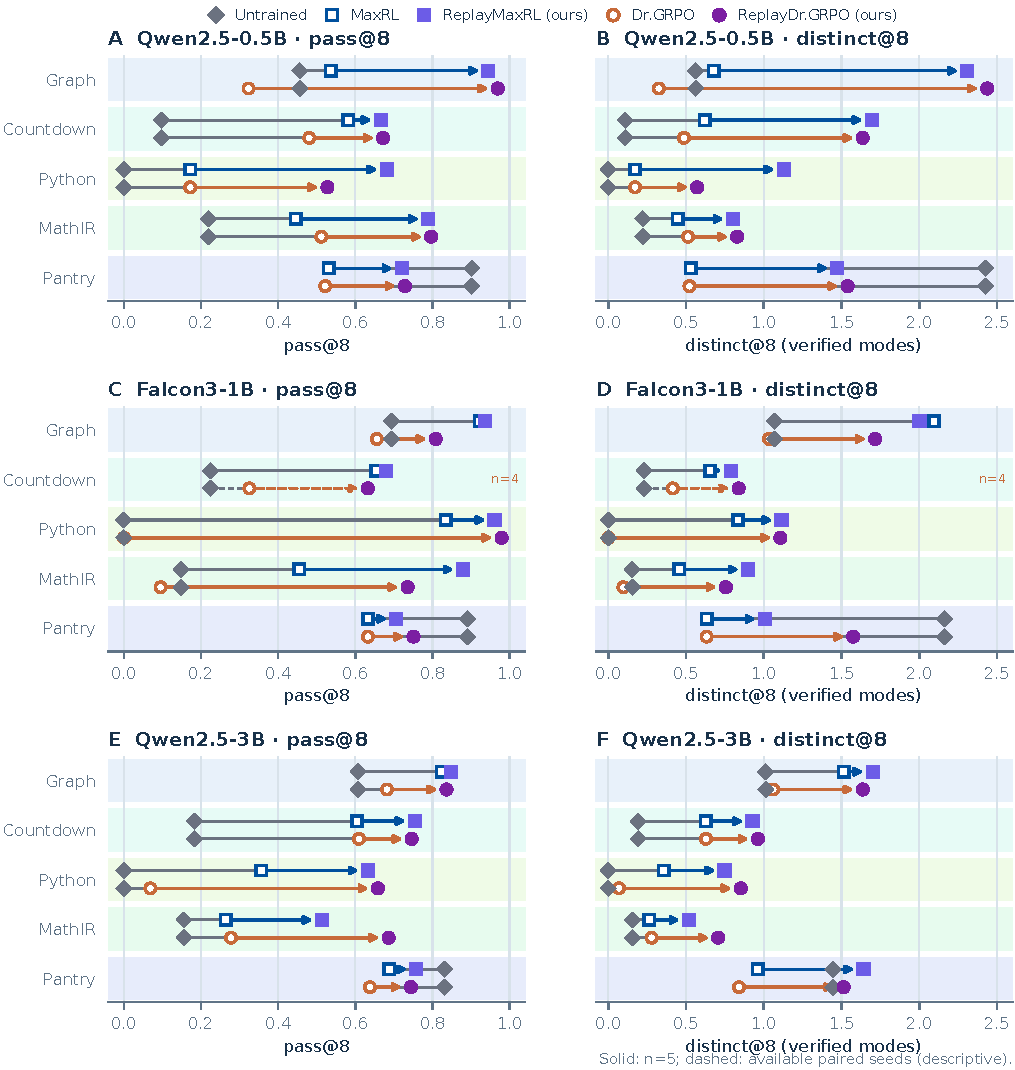
\includegraphics[width=.98\linewidth]
    {figures/e118_scale_extensions_appendix.pdf}
  \caption{\textbf{Replay gains vary by domain and model scale.}
  Final \texttt{pass@8} and \pmd{} at three model scales. Hollow and filled
  markers denote training without and with replay; circles denote Dr.GRPO,
  squares MaxRL, and gray diamonds the model before training. Correctness
  uses five paired seeds except Falcon \texttt{Countdown} Dr.GRPO ($n=4$).
  Diversity averages each arm's eligible seeds separately, requiring at least
  30 eligible prompts per seed. Lines are solid for five control seeds and
  dashed for fewer. Seed counts may differ between arms; estimates below the
  threshold are omitted. Table~\ref{tab:cross-scale-terminal-effects} reports
  paired diversity effects using a 20-prompt threshold. Error bars are omitted.}

  \label{fig:maxrl-factorial-scale-extensions}
\end{figure}


Diversity effects in Fig.~\ref{fig:replay-factorial-effects} and
Table~\ref{tab:cross-scale-terminal-effects} use paired seeds for which
both arms have at least 20 eligible evaluation prompts. The separate-arm
means in Table~\ref{tab:core-terminal-endpoints} and
Fig.~\ref{fig:maxrl-factorial-scale-extensions} instead require 30 eligible
prompts per seed in each arm. Correctness, absolute diversity, and paired
diversity effects can therefore use different seed sets; eligible prompt
subsets can also differ between arms. Diversity-effect intervals use
Student-$t$ with $n-1$ degrees of freedom for $n\ge2$ paired seeds; single-seed
effects have no interval. Correctness and mode-count intervals require five
paired seeds. All intervals are nominal 95\% estimates, without adjustment
for multiple comparisons.

For Qwen2.5-0.5B, Re:Max increases \pmd{} by $+.439$, $+.489$, and
$+.317$ on \texttt{Graph}, \texttt{Countdown}, and \texttt{PantryPlan},
respectively; each five-seed interval excludes zero. Falcon \texttt{Graph}
has a diversity effect of $-.009$ ($[-.034,+.016]$) and a correctness
effect of $+.014$ ($[-.016,+.044]$), both inconclusive. Thus a positive
cross-domain average does not imply improvement in every domain.

For Qwen2.5-3B, the five-seed \pmd{} effects are $+.076$, $+.077$,
$+.058$, $+.006$, and $+.224$ for \texttt{Graph}, \texttt{Countdown},
\texttt{Python}, \texttt{MathIR}, and \texttt{PantryPlan}, respectively.
All diversity intervals exclude zero, although the \texttt{MathIR} effect is
small. Correctness intervals exclude zero for \texttt{Countdown},
\texttt{MathIR}, and \texttt{PantryPlan}, but include zero for \texttt{Graph}
and \texttt{Python}. Across scales, Re:Max exceeds MaxRL in mean \pmd{} in
14 of 15 measurable comparisons; Re:Dr exceeds
Dr.GRPO in 14 of 14. These counts summarize
the signs of the estimated effects, not their statistical significance.

\paragraph{Cross-domain factorial summaries.}
\label{app:factorial-numerical-detail}
Weighting all five domains equally within each paired seed, Re:Max improves
\texttt{pass@8} over MaxRL by $+.307$ at Qwen2.5-0.5B (95\% interval
$[+.208,+.406]$), $+.133$ at Falcon3-1B ($[+.043,+.223]$), and $+.154$
at Qwen2.5-3B ($[+.086,+.222]$). Each comparison uses five seeds. The
corresponding Re:Dr effects are $+.337$, $+.442$, and $+.279$. The Falcon
Dr.GRPO comparison uses four common seeds and has no interval; the other
two use five.

At Qwen2.5-3B, MaxRL and Re:Max have mean correctness $.547$ and $.701$,
and mean \distk{} $.744$ and $1.107$, respectively. Their paired mode-count
difference is $+.363$ ($[+.285,+.441]$). The cross-domain \pmd{} means in
Table~\ref{tab:cross-scale-terminal-effects} use a fixed set of domains
eligible for every contributing seed.

\subsection{Level 1 at Qwen2.5-7B}
\label{app:qwen7b-level1}

We also compare MaxRL and Re:Max at Qwen2.5-7B on Level~1 in
3 domains. The 6 training runs form one
matched treatment--control pair per domain, each trained for
3072 updates with the same prompts, horizon, verifier,
evaluation procedure, and replay schedule as the smaller-scale comparisons.
With one matched seed per domain, these effects are descriptive and have no
confidence intervals.

On \texttt{MathIR}, MaxRL's observed \texttt{pass@8} reaches zero
at update 960 and remains zero at subsequent evaluations.
The final evaluation contains no verified response, so \pmd{} cannot be
estimated. Table~\ref{tab:qwen7b-level1} reports it as undefined rather than
zero. Re:Max, evaluated on the same prompts and seed, reaches
.744 \texttt{pass@8} and .017
\pmd{}. The correctness result remains measurable even though a paired
diversity effect is unavailable.

Where both conditions have measurable diversity, Re:Max increases \pmd{}
by +.298 on \texttt{Graph} and
+.137 on \texttt{Countdown}. These point estimates
exceed the corresponding 3B means, but one seed does not establish a trend
with model scale. Mean \texttt{pass@8} across all 3 domains
is .342 for MaxRL and .789 for Re:Max. Mean
\pmd{} is .028 and .245, respectively, over the
2 domains where both conditions define it. Thus the
correctness mean includes \texttt{MathIR}, while the diversity
mean does not.

\begin{table}[!htbp]
  \centering
  \caption{\textbf{Level-1 correctness and solution diversity at Qwen2.5-7B.}
  Results from 6 runs with 1 matched seed per
  domain after 3072 updates. On \texttt{MathIR},
  MaxRL produces no verified response: its correctness is zero, while its
  \pmd{} and the paired diversity effect are undefined (\texttt{--}).
  Means use 3 domains for correctness and the
  2 jointly eligible domains for diversity. No confidence
  intervals are reported per domain for these single-seed comparisons.}

  \label{tab:qwen7b-level1}
  \small
  \setlength{\tabcolsep}{6pt}
  \begin{tabular}{@{}l*{6}{r}@{}}
    \toprule
    & \multicolumn{2}{c}{\textbf{MaxRL}} & \multicolumn{2}{c}{\textbf{Re:Max}}
      & \multicolumn{2}{c}{\textbf{Re:Max $-$ MaxRL}} \\
    \cmidrule(lr){2-3}\cmidrule(lr){4-5}\cmidrule(lr){6-7}
    \textbf{Domain} & \texttt{pass@8} & \pmd{} & \texttt{pass@8} & \pmd{}
      & \texttt{pass@8} & \pmd{} \\
    \midrule
    % Generated by ops/build_paper_e124_qwen7b_level1.py; do not hand edit.
  \texttt{Countdown} & .631 & .001 & .805 & .138 & +.174 & +.137 \\
  \texttt{Graph} & .396 & .055 & .818 & .353 & +.422 & +.298 \\
  \texttt{MathIR} & .000 & -- & .744 & .017 & +.744 & -- \\
  \midrule
  Mean & .342 & .028 & .789 & .245 & +.447 & +.217 \\
  \bottomrule

  \end{tabular}
\end{table}

\subsection{Results on harder benchmark levels}
\label{app:level2-interim}

\begin{figure}[!htbp]
\centering
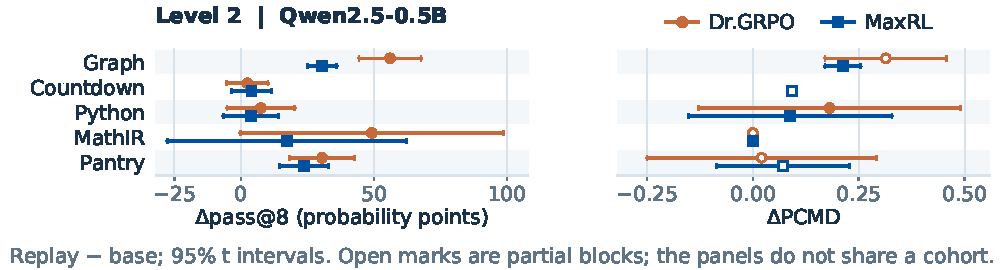
\includegraphics[width=\linewidth]{figures/replay_level2_effects.pdf}
\caption{\textbf{Replay improves Level-2 \texttt{Graph} accuracy and solution diversity.}
Final Re:Dr minus Dr.GRPO (circles) and Re:Max minus MaxRL (squares) effects
for Qwen2.5-0.5B, in percentage points of \texttt{pass@8} and \pmd{} units.
Correctness uses five paired seeds per domain. Diversity requires at least
20 eligible prompts per arm. Re:Dr uses three seeds for \texttt{Graph} and
\texttt{PantryPlan}, four for \texttt{MathIR}, and none for
\texttt{Countdown}; Re:Max uses one for \texttt{Countdown} and four for
\texttt{PantryPlan}. Other comparisons use five. Hollow markers indicate
fewer than five pairs; blanks indicate no eligible pair. Bars show nominal
paired 95\% Student-$t$ intervals for comparisons with at least two seeds.}

  \label{fig:replay-level2-effects}
\end{figure}

Fig.~\ref{fig:level2-admission} compares replay effects across Levels 1--3
using fixed domain sets. Correctness gives equal weight to \texttt{Graph},
\texttt{Countdown}, \texttt{Python}, and \texttt{PantryPlan} within each of
five common training seeds. Diversity first averages eligible seeds within
each arm and domain, then weights \texttt{Graph}, \texttt{MathIR}, and
\texttt{PantryPlan} equally. Its contributing seeds can differ across arms
and levels, so differences between these diversity means are descriptive
and have no intervals. At Level 2, only \texttt{PantryPlan} has sufficient
verified responses before training to estimate diversity; the initial
three-domain diversity mean is therefore undefined.

Each Level-2 method has five final training seeds per domain. The diversity
comparisons in Fig.~\ref{fig:replay-level2-effects} additionally require
eligible prompts in both arms. \texttt{Graph} improves under both objectives:
Re:Max increases \pmd{} by $+.212$ ($[+.170,+.255]$, five seeds), and
Re:Dr by $+.314$ ($[+.170,+.458]$, three seeds). The corresponding
\texttt{Python} effects are $+.088$ and $+.181$, with intervals including
zero; \texttt{MathIR} effects are near zero. \texttt{PantryPlan}
correctness improves by $+.305$ under Re:Dr and $+.237$ under Re:Max,
each measured over five seeds.

Each Level-2 \texttt{MathIR} prompt admits one shortest derivation and four
longer alternatives. Concentration on the shortest route therefore yields
near-zero diversity despite the existence of other valid modes. The levels
also use different held-out problems and can differ in mode-count
distributions and prompt guidance (App.~\ref{app:data-levels}). Cross-level
comparisons consequently do not isolate the causal effect of difficulty.

For each common seed and endpoint $Y$, the replay interaction is
\[
 I=(Y^{\rm Re:Max}-Y^{\rm MaxRL})
    -(Y^{\rm Re:Dr}-Y^{\rm Dr.GRPO}).
\]
A negative interaction means that replay adds less under MaxRL than under
Dr.GRPO; it does not imply that replay harms MaxRL. On Level-2
\texttt{Graph}, MaxRL alone improves \texttt{pass@8} over Dr.GRPO by
$+.233$ ($[+.140,+.325]$), while the replay interaction is $-.256$
($[-.329,-.183]$). Replay improves both objectives, with a smaller
additional benefit under the stronger fresh objective.

\begin{table}[!htbp]
  \centering
  \caption{\textbf{A stronger fresh objective need not increase the additional benefit of replay.}
  Contrasts use five common seeds per domain across all four methods.
  The interaction is
  $(\mathrm{Re:Max}-\mathrm{MaxRL})-(\mathrm{Re:Dr}-\mathrm{Dr.GRPO})$.
  Here $P_8=\texttt{pass@8}$, $D_8=\texttt{distinct@8}$, and $B_8=D_8-P_8$.
  Entries report paired means and nominal 95\% Student-$t$ intervals. Both
  mode-count metrics depend on correctness. The conditional-diversity analysis
  in Fig.~\ref{fig:replay-level2-effects} applies separate eligibility
  requirements, so its seed populations can differ from those in this table.}

\label{tab:level2-factorial-contrasts}
  \scriptsize
  \setlength{\tabcolsep}{3pt}
  \resizebox{\linewidth}{!}{%
  \begin{tabular}{@{}lclrrr@{}}
    \toprule
    \textbf{Domain} & $n$ & \textbf{Contrast} &
    $\Delta P_8$ & $\Delta D_8$ & $\Delta B_8$ \\
    \midrule
    % Domain & paired n & contrast & delta pass@8 & delta distinct@8 & delta extra modes
Graph & 5 & MaxRL $-$ Dr.GRPO & $+.233\;[+.140,+.325]$ & $+.322\;[+.162,+.482]$ & $+.089\;[+.019,+.159]$ \\
Graph & 5 & Re:Max $-$ Re:Dr & $-.023\;[-.062,+.016]$ & $-.029\;[-.198,+.140]$ & $-.006\;[-.142,+.130]$ \\
Graph & 5 & Replay $\times$ MaxRL interaction & $-.256\;[-.329,-.183]$ & $-.351\;[-.446,-.255]$ & $-.095\;[-.186,-.003]$ \\
Countdown & 5 & MaxRL $-$ Dr.GRPO & $-.014\;[-.073,+.045]$ & $-.014\;[-.073,+.045]$ & $+.000\;[+.000,+.000]$ \\
Countdown & 5 & Re:Max $-$ Re:Dr & $+.002\;[-.008,+.012]$ & $-.002\;[-.047,+.044]$ & $-.004\;[-.042,+.035]$ \\
Countdown & 5 & Replay $\times$ MaxRL interaction & $+.016\;[-.047,+.078]$ & $+.012\;[-.068,+.092]$ & $-.004\;[-.042,+.035]$ \\
Python & 5 & MaxRL $-$ Dr.GRPO & $+.000\;[+.000,+.000]$ & $+.000\;[+.000,+.000]$ & $+.000\;[+.000,+.000]$ \\
Python & 5 & Re:Max $-$ Re:Dr & $-.037\;[-.232,+.157]$ & $-.188\;[-.988,+.613]$ & $-.150\;[-1.014,+.713]$ \\
Python & 5 & Replay $\times$ MaxRL interaction & $-.037\;[-.232,+.157]$ & $-.188\;[-.988,+.613]$ & $-.150\;[-1.014,+.713]$ \\
MathIR & 5 & MaxRL $-$ Dr.GRPO & $+.283\;[-.193,+.759]$ & $+.283\;[-.193,+.759]$ & $+.000\;[+.000,+.000]$ \\
MathIR & 5 & Re:Max $-$ Re:Dr & $-.036\;[-.158,+.085]$ & $-.035\;[-.158,+.088]$ & $+.002\;[-.003,+.006]$ \\
MathIR & 5 & Replay $\times$ MaxRL interaction & $-.320\;[-.864,+.225]$ & $-.318\;[-.860,+.224]$ & $+.002\;[-.003,+.006]$ \\
PantryPlan & 5 & MaxRL $-$ Dr.GRPO & $+.019\;[-.067,+.105]$ & $+.019\;[-.081,+.119]$ & $+.000\;[-.021,+.021]$ \\
PantryPlan & 5 & Re:Max $-$ Re:Dr & $-.049\;[-.113,+.014]$ & $-.061\;[-.249,+.128]$ & $-.012\;[-.145,+.122]$ \\
PantryPlan & 5 & Replay $\times$ MaxRL interaction & $-.068\;[-.168,+.032]$ & $-.080\;[-.279,+.119]$ & $-.012\;[-.134,+.110]$ \\
    \bottomrule

  \end{tabular}}
\end{table}


\paragraph{Level-2 \texttt{Graph} results.}
\label{app:levels-numerical-detail}
Before training, Qwen2.5-0.5B \texttt{Graph} \texttt{pass@8} is $.438$
on the Level-1 development split and $.148$ on Level 2. After eight Level-2
training passes, Dr.GRPO and MaxRL reach $.202$ and $.434$, compared
with $.763$ and $.739$ for Re:Dr and Re:Max. The paired correctness gains
are $+.561$ and $+.305$, with 95\% Student-$t$ intervals $[+.445,+.677]$
and $[+.250,+.360]$ over five seeds each. The lowest replay accuracy
($.711$) exceeds the highest accuracy without replay ($.477$). Replay adds
$1.019$ and $.668$ distinct verified modes for the two objectives,
respectively, yielding \texttt{distinct@8} of $1.243$ and $1.214$.

For the three eligible Dr.GRPO seed pairs, \pmd{} rises from $.039$ to
$.353$; for the five MaxRL pairs, it rises from $.112$ to $.325$.
Expressed on the effective-mode scale, these changes are $1.04$ to $1.55$
and $1.13$ to $1.48$, corresponding to ratios of $1.49$ and $1.32$.
Relative increases in \pmd{} are unstable near a zero baseline, so we
report absolute changes instead. The joint improvements in correctness and
diversity do not establish that greater diversity causes better correctness.

\subsection{Accuracy and verified modes throughout training}
\label{app:factorial-training-curves}

Figs.~\ref{fig:factorial-training-accuracy}--\ref{fig:level2-training-pmd}
show correctness and diversity throughout training, using four groups of
eight responses to each of 128 held-out prompts. Lines show seed means;
bands show the range across seeds, rather than confidence intervals. A seed
contributes to conditional diversity only when at least five prompts have
two or more correct responses. The contributing seeds and prompts can
therefore change across methods and checkpoints.

\begin{figure}[!htbp]
  \centering
  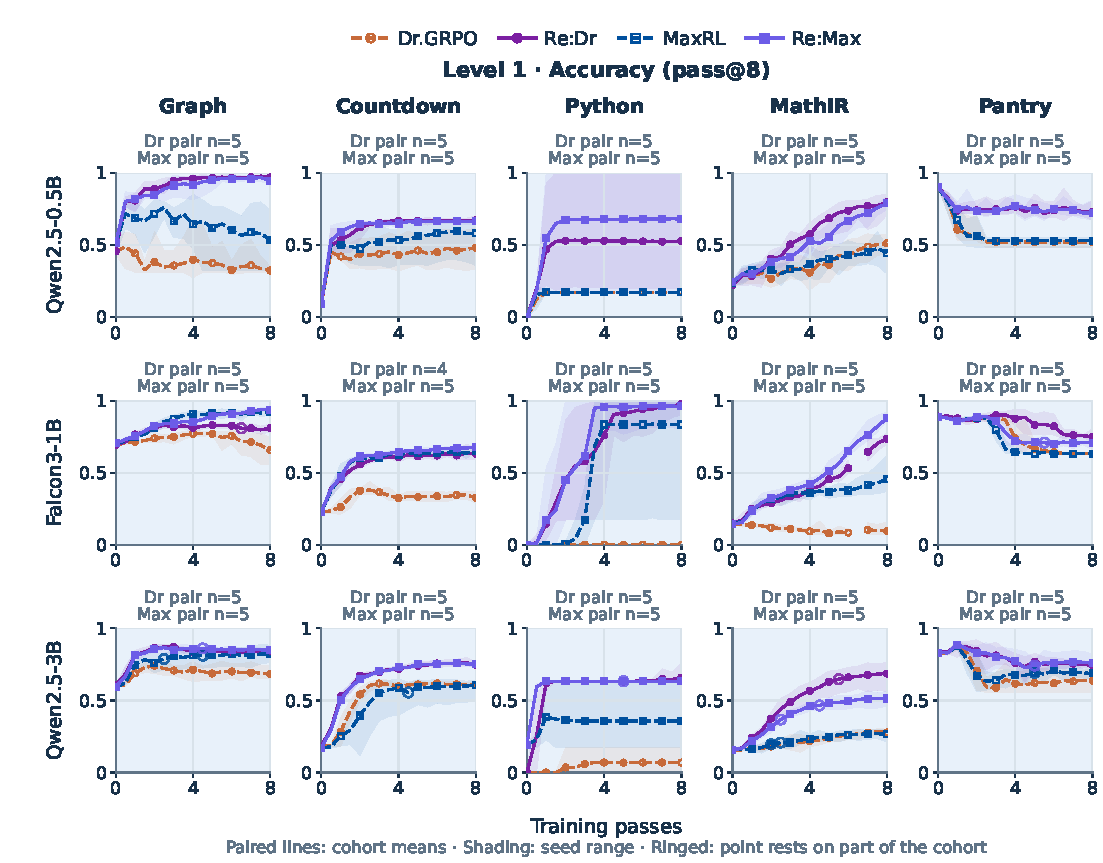
\includegraphics[width=\linewidth]{figures/factorial_training_curves_pass8.pdf}
  \caption{\textbf{Replay improves final accuracy across model scales.}
  \texttt{pass@8} over eight training passes for Dr.GRPO, Re:Dr, MaxRL, and
  Re:Max. Rows show Qwen2.5-0.5B, Falcon3-1B, and Qwen2.5-3B; columns show
  domains. Panel labels give the numbers of paired seeds at the final
  checkpoint. Lines show seed means and bands show seed ranges, rather than
  confidence intervals. Ringed points use fewer seeds than the final comparison.}

  \label{fig:factorial-training-accuracy}
\end{figure}

\begin{figure}[!htbp]
  \centering
  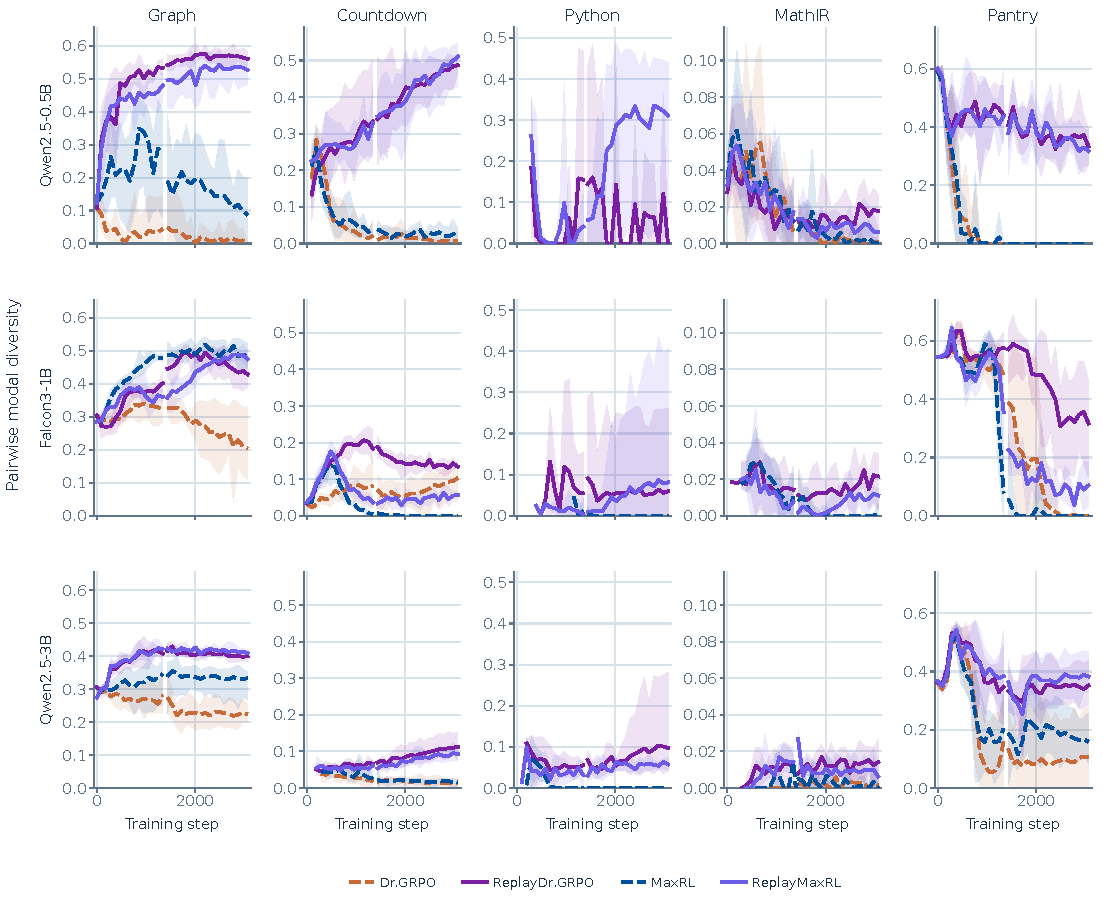
\includegraphics[width=\linewidth]{figures/factorial_training_curves_pmd.pdf}
  \caption{\textbf{Replay limits the loss of \texttt{PantryPlan} solution diversity at every scale.}
\pmd{} throughout training, with model rows and method colours as in
Fig.~\ref{fig:factorial-training-accuracy}. Both fresh objectives reach zero
terminal \texttt{PantryPlan} diversity at 0.5B and 1B, whereas both replay variants
retain multiple solution modes. Lines average one to five eligible seeds
per checkpoint; bands show seed ranges and are absent for a single seed.
A seed contributes when at least five prompts yield at least two correct responses.
Fine dotted segments use fewer seeds, so changes can reflect sample
composition. Gaps indicate undefined estimates. Vertical scales are shared
within each domain.}
  \label{fig:factorial-training-modes}
\end{figure}

\begin{figure}[!htbp]
  \centering
  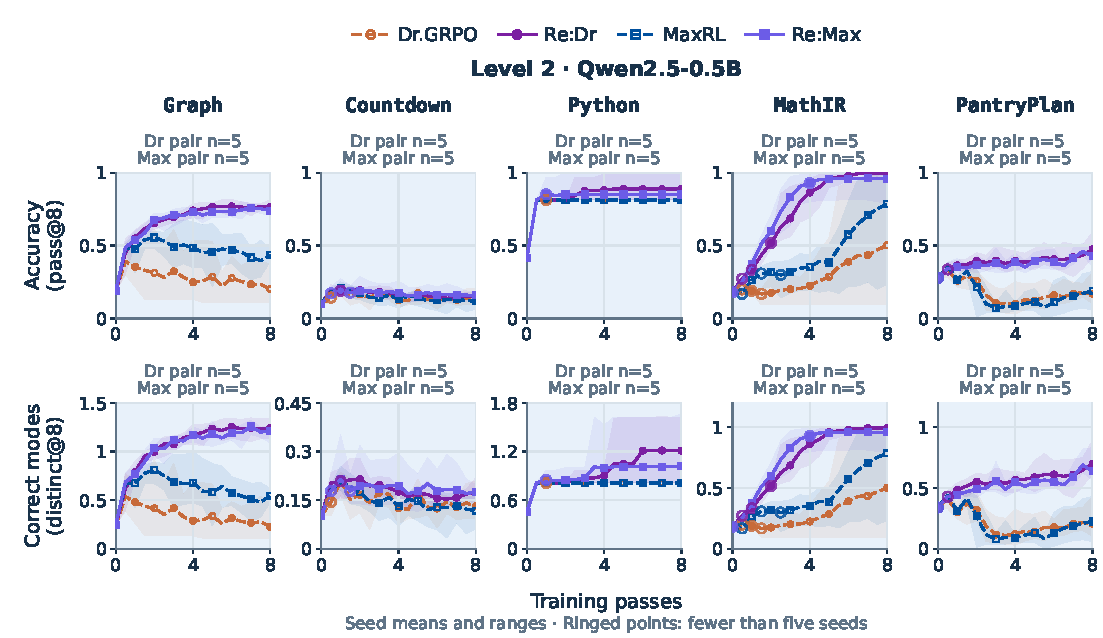
\includegraphics[width=\linewidth]{figures/level2_factorial_training_curves.pdf}
  \caption{\textbf{Replay improves final accuracy and verified-mode counts at Level~2.}
Qwen2.5-0.5B trajectories for Dr.GRPO, Re:Dr, MaxRL, and Re:Max across five
domains. Rows show \texttt{pass@8} and \distk{}; the latter depends on both
correctness and solution diversity. Each objective pair has five matched
seeds at the terminal checkpoint. Lines show seed means and bands show
seed ranges. Ringed points use fewer than five seeds; Fig.~\ref{fig:level2-training-pmd}
reports success-conditional diversity.}
  \label{fig:level2-training-curves}
\end{figure}

\begin{figure}[!htbp]
  \centering
  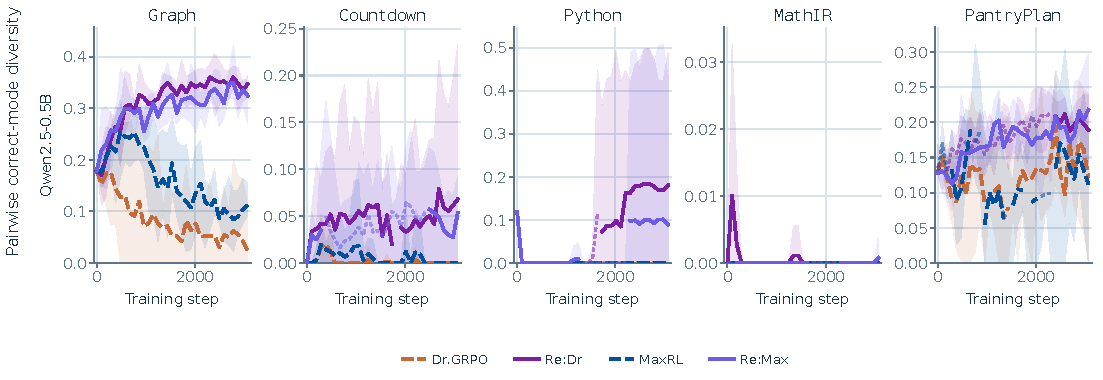
\includegraphics[width=\linewidth]{figures/level2_training_curves_pmd.pdf}
  \caption{\textbf{Replay preserves greater solution diversity on Level-2 \texttt{Graph}.}
\pmd{} during Qwen2.5-0.5B training for the four primary methods. At the
terminal checkpoint, Re:Dr and Re:Max reach $.346$ and $.325$, compared with
$.023$ for Dr.GRPO and $.112$ for MaxRL. \texttt{MathIR} remains near zero under all
four methods. Lines average eligible seeds and bands show seed ranges.
Each seed requires at least five prompts with at least two correct responses.
Fine dotted segments indicate fewer contributing seeds, and gaps indicate that the estimate is undefined.}
  \label{fig:level2-training-pmd}
\end{figure}


\subsection{Supporting comparators}
\label{app:ucpo-progress}

GRPO normalizes rewards within each group; UCPO redistributes the advantage
among fresh on-policy responses; sparse RLEP-Dr reuses verified successes
without uniform weighting by canonical key. We evaluate GRPO in 75 training
runs across three model scales. UCPO and RLEP-Dr cover the two smaller
scales, with 50 and 47 runs, respectively. RLEP-Dr uses two seeds for Falcon
\texttt{Python} and five elsewhere. Fixed Semantic-MaxEnt adds a
frequency-based bonus to fresh responses (App.~\ref{app:semantic-maxent}).
Its four-method factorial covers ten model--domain combinations at the two
smaller scales, with five common seeds except Falcon \texttt{Countdown}
($n=4$). The 3B comparison uses one seed to evaluate adding the bonus to
replay (App.~\ref{app:semantic-current-factorial}).

For GRPO, UCPO, and RLEP-Dr, the diversity contrasts in this subsection
average per-prompt differences over prompts with at least two correct
responses in both arms. Each seed must have at least 30 such jointly
eligible prompts. Table~\ref{tab:direct-comparator-matrix} instead uses
separate 20-prompt thresholds for each arm. On Qwen2.5-0.5B \texttt{Graph},
one UCPO seed and four RLEP-Dr seeds meet the joint criterion; no
\texttt{Python} comparison meets it at any scale.

For Qwen2.5-0.5B, UCPO improves \texttt{Countdown} \texttt{pass@8} by
$+.133$ ($[+.005,+.262]$), while its \pmd{} effect is inconclusive:
$+.002$ ($[-.018,+.023]$). Its \texttt{MathIR} effects are also
inconclusive. RLEP-Dr improves \texttt{MathIR} correctness by $+.126$
($[+.030,+.222]$), with zero measured diversity change; its
\texttt{Countdown} and Falcon \texttt{PantryPlan} effects are inconclusive.
Across GRPO, UCPO, and RLEP-Dr, seven of 34 five-seed correctness intervals
lie above zero. None of the 19 five-seed diversity intervals lies above zero; one lies
below zero, for Falcon \texttt{Countdown} GRPO: $-.105$
($[-.147,-.063]$). At Qwen2.5-3B, all five GRPO correctness intervals and
the three available diversity intervals include zero. These are nominal
paired 95\% Student-$t$ intervals over training seeds.

The uniform versus frequency-weighted replay comparison uses five paired
seeds in each of nine model--domain combinations: all five Qwen2.5-0.5B
domains, plus \texttt{Graph} and \texttt{PantryPlan} at both larger scales.
Changing only the within-buffer weights increases extra verified modes by
$+.318$ per prompt in the Qwen2.5-0.5B average ($[+.272,+.358]$,
paired-seed bootstrap). The correctness effect is inconclusive at $+.010$
($[-.119,+.139]$). This result supports a benefit from uniform weighting
beyond reusing successful responses in proportion to their frequency,
although extra-mode counts still depend on correctness
(App.~\ref{app:frequency-replay-progress}).

RLEP-Dr's offline response pool uses temperature $.7$ and top-$p=.95$;
evaluation uses temperature 1 and top-$p=1$. Its offline data collection
also differs from the online construction of prompt-specific verified replay
buffers, and the next paragraph measures what that difference puts in the pool.

\paragraph{What RLEP-Dr replays.}
\phantomsection\label{app:rlep-pool}
RLEP's protocol harvests its experience pool from a policy that RL has
already trained \citep{zhang2025rlep}: the seed policy samples 64 candidates
per prompt at temperature $.7$ and top-$p=.95$, verified answers are kept, and
a prompt enters the pool only with at least two of them. Here the seed policy
is the paired terminal Dr.GRPO control, so the pool is a sample from the
collapsed endpoint that Sec.~\ref{sec:results-collapse} measures.
Table~\ref{tab:rlep-pool-composition} reads the frozen pools and the learner
telemetry of every RLEP-Dr cell. At Qwen2.5-0.5B,
43\%--79\% of the 384 training prompts hold
no verified trajectory and never receive a replay row. Of the
4393 eligible prompts pooled over all 25
cells, all but 17 hold a single canonical key among
their verified trajectories, and none holds more than 2, so a
two-row replay draw is two copies of one mode with probability at least
.99 in every domain.
Falcon3-1B pools are slightly wider on \texttt{Graph} and \texttt{Countdown},
up to 1.40 keys per eligible prompt, and a same-mode pair
remains the draw with probability
.89--1.00. The online Re:Dr buffer on the
same prompts and seeds holds 2.6--6.9 modes on average
in the three domains where modes are plentiful. RLEP-Dr's replay is therefore
single-mode replay of the control's own endpoint, applied on
21\%--57\% of updates, and its \pmd{} beside the
control is the expected outcome rather than a discrepancy with Re:Dr: no
update rule rehearses a second mode from a pool that holds one.

The two update rules are closer than their descriptions suggest. RLEP's
replay row enters the policy gradient with advantage $1-\bar r$, where
$\bar r$ is the mean reward of the mixed group, so it is a positive-coefficient
log-likelihood term on a stored success, as Re:Dr's replay term is. The
difference is that RLEP's coefficient shrinks toward zero as the prompt is
solved, with a realized mean of .03--.38 across domains
at 0.5B, whereas Re:Dr's is fixed. Whether a likelihood term on a single
stored success can produce breadth is tested directly by the capacity-one arm
of App.~\ref{app:mode-agnostic-replay}, which applies exactly such a term to
one success captured online at first discovery and recovers 58\% of
the Re:Dr effect. What separates the two replay families is thus not the loss
but the buffer: what it stores, from which policy, and from when.

\begin{table}[H]
  \centering
  \caption{\textbf{RLEP-Dr's pools hold one mode per prompt.} Composition of
  the frozen RLEP experience pools and the realized replay dose, averaged over
  seeds. \emph{none} is the share of the 384 training prompts with no verified
  trajectory; \emph{eligible} the share with at least two; \emph{keys} the mean
  number of canonical modes among an eligible prompt's verified trajectories;
  $P(\text{same})$ the probability that a two-row replay draw repeats one
  mode; \emph{updates} the share of optimizer updates that mixed in replay
  rows; $A_{\text{replay}}$ the mean replay advantage $1-\bar r$ on those
  updates. The last column is the mean number of modes in the Re:Dr buffer
  over the within-cohort cells on the same prompts and seeds
  (Tab.~\ref{tab:matched-redr}).}
  \label{tab:rlep-pool-composition}
  \small
  \setlength{\tabcolsep}{5pt}
  \begin{tabular}{@{}lrrrrrrrr@{}}
    \toprule
    \textbf{Domain} & $n$ & \textbf{none} & \textbf{eligible} & \textbf{keys}
      & $P(\text{same})$ & \textbf{updates} & $A_{\text{replay}}$
      & \textbf{Re:Dr modes} \\
    \midrule
    % Generated by ops/build_paper_rlep_pool_composition.py; do not hand edit.
  \multicolumn{9}{@{}l}{\textit{Qwen2.5-0.5B}} \\
  \texttt{Graph} & 5 & 64\% & 36\% & 1.00 & 1.00 & 36\% & .19 & 3.77 \\
  \texttt{Countdown} & 5 & 43\% & 57\% & 1.02 & .99 & 57\% & .11 & 2.56 \\
  \texttt{Python} & 5 & 79\% & 21\% & 1.00 & 1.00 & 21\% & .03 & 1.20 \\
  \texttt{MathIR} & 5 & 43\% & 57\% & 1.00 & 1.00 & 57\% & .38 & 1.15 \\
  \texttt{PantryPlan} & 5 & 43\% & 57\% & 1.00 & 1.00 & 57\% & .03 & 6.88 \\
  \multicolumn{9}{@{}l}{\textit{Falcon3-1B}} \\
  \texttt{Graph} & 5 & 44\% & 56\% & 1.40 & .89 & 56\% & .41 & \textemdash{} \\
  \texttt{Countdown} & 5 & 56\% & 44\% & 1.17 & .95 & 44\% & .24 & \textemdash{} \\
  \texttt{Python} & 2 & 90\% & 10\% & 1.01 & 1.00 & 10\% & .50 & \textemdash{} \\
  \texttt{MathIR} & 5 & 91\% & 9\% & 1.01 & 1.00 & 9\% & .30 & \textemdash{} \\
  \texttt{PantryPlan} & 5 & 41\% & 59\% & 1.00 & 1.00 & 59\% & .09 & \textemdash{} \\
  \bottomrule

  \end{tabular}
\end{table}

\paragraph{Comparator settings.}
\phantomsection\label{app:comparator-settings}
Each comparator shares the non-objective settings of its paired control
(Table~\ref{tab:run-contract}). UCPO uses the published default
$\omega=.2$, and RLEP-Dr uses the published combination of 16 fresh and
2 replay responses. GAPO has no free coefficient; its reward is affinely
mapped to the control's unit range because Dr.GRPO does not normalize by
the group standard deviation. SetPO uses $\lambda=1.0$, giving a diversity
term approximately 5.3\% of the task advantage; its paper provides no
coefficient for the 0.5B verifier-reward setting. Semantic-MaxEnt uses
$\eta=.10$ and $\kappa=5$. Replay uses $\lambda_{\mathrm{replay}}=.10$
and capacity $M=16$, equal to the rollout group size. These settings are
not tuned to \mb{} outcomes, and no method receives a learning-rate sweep.
The results therefore compare the methods at the stated settings;
hyperparameter tuning could improve correctness or diversity.

\paragraph{Interpreting zero diversity.}
In Table~\ref{tab:direct-comparator-matrix}, an em-dash denotes an undefined
paired difference. An exact $.000$ instead denotes a measured zero, with
identical values for both methods in every eligible seed. The
\texttt{Python} \pmd{} column contains measured zeros because, for each
eligible prompt, both methods' verified responses share a single execution
key. High correctness can coexist with this concentration: four of the five
SetPO \texttt{Python} seeds reach \texttt{pass@8} $1.000$ and terminal
\pmd{} $.000$. Every held-out prompt has at least one correct response,
but the verified responses for each prompt use a single mode. Per-response
correctness also increases in all 15 control comparisons
(App.~\ref{app:control-learning-audit}).

\begin{figure}[!htbp]
  \centering
  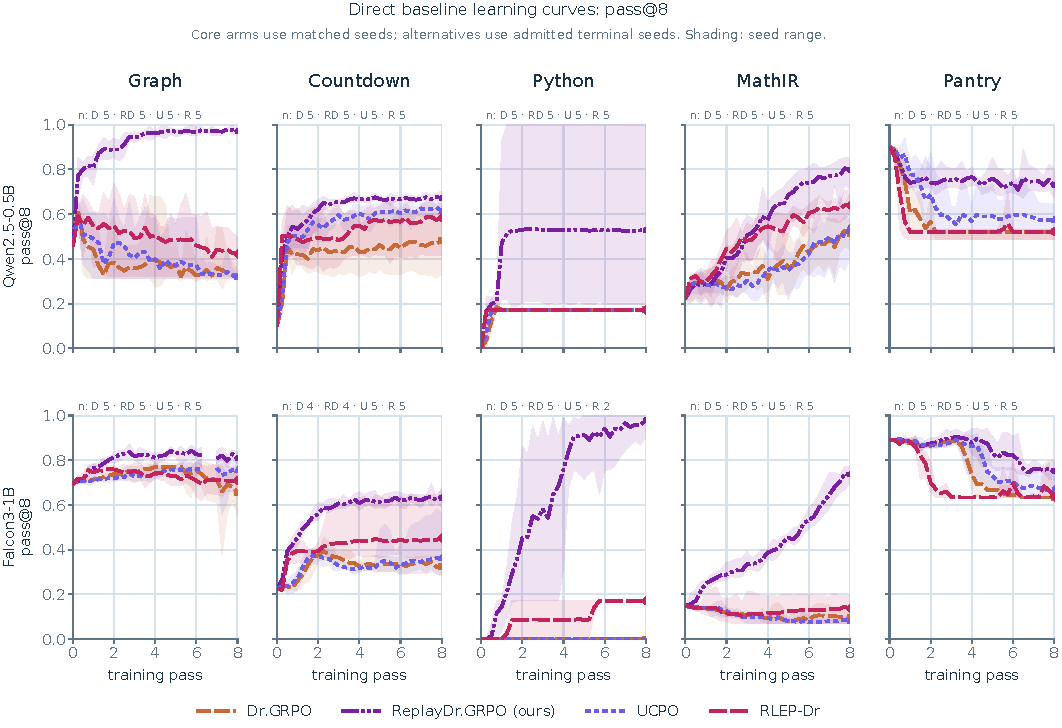
\includegraphics[width=\linewidth]{figures/direct_baseline_learning_curves_pass8.pdf}
  \caption{\textbf{Re:Dr has the highest terminal mean accuracy in every
  displayed comparison.} \texttt{pass@8} during Level-1 training for Dr.GRPO,
  Re:Dr, UCPO, and sparse RLEP-Dr. Rows show Qwen2.5-0.5B and Falcon3-1B;
  columns show the five domains. Lines show seed means and bands show seed
  ranges; gaps indicate unavailable estimates. Dr.GRPO and Re:Dr use paired
  seeds. Comparisons use five seeds except Falcon \texttt{Countdown}
  Dr.GRPO/Re:Dr ($n=4$) and Falcon \texttt{Python} RLEP-Dr ($n=2$), as indicated in the panels.}
  \label{fig:direct-baseline-accuracy-curves}
\end{figure}


\subsection{Diversity-preserving comparators}
\label{app:diversity-comparators}

GAPO~\citep{anschel2025groupaware} and SetPO~\citep{li2026setpo} target
output diversity within the fresh rollout group. Both are evaluated on
Level-1 Qwen2.5-0.5B across five domains and five seeds. GAPO assigns
verifier-positive rollouts the reward $[1-(f_i-1/L)+1]/2$, with zero for
failures, where $f_i$ is the key's frequency among the group's verified
rollouts and $L$ is the prompt's certified number of valid modes.
SetPO augments each rollout's advantage by its marginal contribution to
kernelized set diversity, measured by removing that rollout from the group,
with coefficient $\lambda=1$. It computes similarities using a fixed
\texttt{all-MiniLM-L6-v2} sentence encoder, mean pooling, and cosine
similarity clamped to $[0,1]$. Encoding the responses adds computation.

GAPO increases \pmd{} on \texttt{Countdown} ($+.340$, $[+.112,+.567]$) and \texttt{PantryPlan}
($+.653$, $[+.610,+.696]$), while its \texttt{Python} effect is near zero
with an interval spanning zero. \texttt{Python} has more valid modes than the
sixteen-rollout group can represent on 95\% of training prompts, with up to 3,600
modes. This limits within-group coverage but does not prevent a policy from
assigning mass across the full support. \texttt{MathIR} effects are small across
methods; the largest is Re:Dr's $+.017$ ($[+.003,+.031]$).
SetPO increases \pmd{} on \texttt{PantryPlan} ($+.266$, $[+.177,+.356]$); its other
four domain intervals include zero. Five-domain mean effects are $+.225$
for GAPO, $+.066$ for SetPO, and $+.320$ for Re:Max, although GAPO's
\texttt{PantryPlan} effect is larger than Re:Max's. The effective number
of modes, $\neff$, on \texttt{PantryPlan} is $2.88$ for GAPO and $1.36$
for SetPO, compared with $1.00$ for their shared control. SetPO also raises
\texttt{Python} \texttt{pass@8} from $.338$ to $.834$, a relative increase
of $147\%$. Relative changes in \pmd{} are undefined for \texttt{PantryPlan}
and \texttt{Python} because the control has $\pmd=.000$. GAPO adjusts
rewards using frequencies within the fresh rollout group, whereas replay
balances the likelihood term across verified modes accumulated in the buffer.

GAPO and SetPO share a Dr.GRPO control with matching hardware and
nonoverlapping evaluation draws. Its terminal \pmd{} differs from the
Dr.GRPO control used in the main replay comparison by a mean of $+.003$
over twenty paired comparisons, ranging from $-.014$ to $+.034$. These
observed differences are small relative to the five-domain effects above,
but do not establish equivalence between the controls.

\subsection{Measured KL tradeoffs and replay occupancy}
\label{app:kl-measured}

Table~\ref{tab:reference-kl-measured} compares terminal \pmd{} at
Qwen2.5-0.5B, Level~1, after $3{,}072$ updates. Dr.GRPO with reference KL
uses 6 coefficients, $\beta\in\{0.001, 0.01, 0.04, 0.1, 0.2, 0.3\}$, across
5 domains. These arms use the zero-replay-derivative control
configuration with a nonzero KL coefficient and the initial policy as the
reference. The comparisons match optimizer updates and fresh-rollout
budgets. They do not equalize total computation: reference-policy evaluation
and replay processing incur different costs, and the control does not spend
those costs on additional effective updates or fresh rollouts.

\begin{figure}[t]
  \centering
  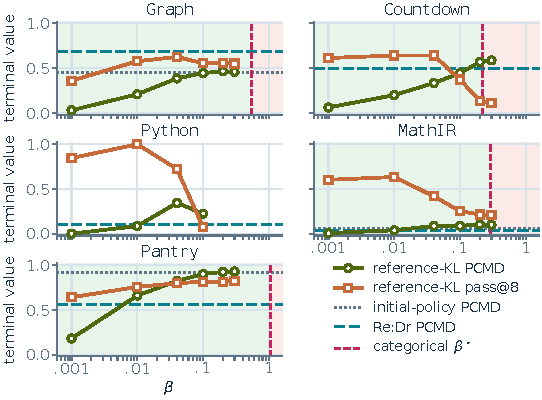
\includegraphics[width=0.78\linewidth]{figures/reference_kl_knee.pdf}
  \caption{\textbf{KL coefficient effects vary by domain.}
  Circles show terminal \pmd{} and squares show \texttt{pass@8} for
  Qwen2.5-0.5B at Level~1; lines connect seed means without uncertainty
  bands. Horizontal rules mark the initial policy's reportable \pmd{}
  (dotted) and Re:Dr's terminal \pmd{} (dashed). Vertical rules mark the
  categorical plug-in threshold $\beta^\star$; green and red indicate
  stationary single-draw correctness above and below one half under that
  calculation. This threshold does not predict the location of the observed
  \texttt{pass@8} knee.}
  \label{fig:reference-kl-knee}
\end{figure}

\paragraph{Initial concentration and coefficient dependence.}
Dr.GRPO without KL reaches \pmd{} at or below $.004$ in all five domains.
MaxRL without replay reaches $.148$ in \texttt{Graph} and at or below $.022$
elsewhere. These low values are consistent with concentration, but the
neural runs do not satisfy the independent-logit assumptions of
Proposition~\ref{thm:grpo-collapse}.
KL produces larger conditional-diversity estimates at several coefficients
in every domain. The response is not uniformly monotone: \texttt{Graph} changes
from $.465$ to $.458$ and \texttt{MathIR} from $.103$ to $.099$ between
$\beta=.2$ and $.3$, while \texttt{Python} changes from $.344$ to $.225$ between
$\beta=.04$ and $.1$.
These are comparisons of point estimates, without a seed-level uncertainty
analysis for their differences.

\begin{table}[t]
  \centering
  \caption{\textbf{KL and replay have different domain-level tradeoffs.}
  Terminal \pmd{} seed means for Qwen2.5-0.5B, Level~1. Superscripts give
  counts below five seeds; dashes indicate unavailable cells. The four
  zero-KL arms use 32 disjoint evaluation streams; KL arms use their own
  disjoint draws with the same estimator. Reference summaries are
  initial-policy \pmd{} and $1-1/\bar k$ for each replay arm, where $\bar k$
  is the mean number of keys replayed per measured update. These do not bound
  neural diversity. The final column computes categorical $\beta^\star$
  from mean initial single-draw correctness.}
  \label{tab:reference-kl-measured}
  \scriptsize
  \setlength{\tabcolsep}{2.5pt}
  \begin{tabular}{@{}lrrrrrrrrrrrrrr@{}}
    \toprule
    & \multicolumn{2}{c}{\textbf{without replay}}
      & \multicolumn{6}{c}{\textbf{$+$ reference KL, by $\beta$}}
      & \multicolumn{2}{c}{\textbf{$+$ replay}}
      & \multicolumn{3}{c}{\textbf{reference summaries}} & \\
    \cmidrule(lr){2-3}\cmidrule(lr){4-9}\cmidrule(lr){10-11}\cmidrule(lr){12-14}
    \textbf{Domain} & Dr.GRPO & MaxRL
      & $.001$ & $.01$ & $.04$ & $.1$ & $.2$ & $.3$
      & \textbf{Re:Dr} & \textbf{Re:Max}
      & Initial & Re:Dr & Re:Max & $\beta^\star$ \\
    \midrule
    % Generated by ops/build_reference_kl_comparison.py; do not hand edit.
  \texttt{Graph}  &  0.003  &  0.148  &  0.029  &  0.207  &  0.385  &  0.444  &  0.465  &  0.458  &  0.686  &  0.625  &  0.45  &  0.75  &  0.70  &  0.55 \\
  \texttt{Countdown}  &  0.004  &  0.022  &  0.060  &  0.198  &  0.333  &  0.444  &  0.568  &  0.587  &  0.497  &  0.531  &  ---  &  0.56  &  0.52  &  0.22 \\
  \texttt{Python}  &  0.000  &  0.000  &  0.000  &  0.086  &  0.344  &  0.225$^{3}$  &  ---  &  ---  &  0.099  &  0.239  &  ---  &  0.15  &  0.42  &  --- \\
  \texttt{MathIR}  &  0.003  &  0.008  &  0.007  &  0.038  &  0.086  &  0.088  &  0.103  &  0.099  &  0.039  &  0.018  &  0.06  &  0.15  &  0.12  &  0.29 \\
  \texttt{Pantry}  &  0.000  &  0.000  &  0.180  &  0.660  &  0.824  &  0.901  &  0.925  &  0.931  &  0.557  &  0.556  &  0.91  &  0.85  &  0.85  &  1.05 \\
  \bottomrule

  \end{tabular}
\end{table}

\paragraph{Stationary predictions and measured checkpoints.}
Proposition~\ref{prop:kl-stationary} identifies the categorical interior
stationary conditional as $q^\star=\mu|_{\mathcal C}$, independently of
$\beta$. It does not bound transient diversity or establish that a finite
neural checkpoint reaches this conditional. The measured \pmd{} varies
with $\beta$ and can exceed the initial estimate: at $\beta=.2$, \texttt{Graph}
reaches $.465$ against $.454$ initially, \texttt{MathIR} $.103$ against $.061$,
and \texttt{Pantry} $.925$ against $.913$. These estimates also condition on each
policy's own verified responses, rather than on a common set of solved
prompts.

For a fixed prompt with $0<\mu(\mathcal C)<1/2$, the Dr.GRPO formula gives
\[
  \beta^\star=\frac{(G-1)/G}{-\operatorname{logit}\mu(\mathcal C)},
  \qquad P^\star(\beta^\star)=\tfrac12.
\]
The displayed values substitute each domain's mean initial correctness
and $G=16$, giving $0.22$--$1.05$.
This aggregation is descriptive: substituting a mean into the nonlinear
stationary formula does not give the mean of its promptwise predictions.
Moreover, $P^\star$ is single-draw correctness, whereas the plotted
\texttt{pass@8} measures success within eight responses. Declines in that
metric already occur below the displayed threshold: \texttt{MathIR} falls from
$.634$ at $\beta=.01$ to $.418$ at $.04$, well below its
$\beta^\star\simeq.29$. \texttt{Countdown} similarly falls from $.642$ at $.04$
to $.372$ at $.1$, below $.22$. The thresholds therefore do not locate
the measured knees. \texttt{Python} has zero observed initial successes, so no
finite plug-in threshold or reportable initial \pmd{} is shown; this
does not establish zero population correctness.

Finite training, shared parameters, prompt sampling, and the adaptive
optimizer can all separate the measured neural trajectory from the
categorical stationary calculation. The comparison does not identify their
individual effects. The boundary-force identities and the two-mode
$\Theta(1/[s\log(1/s)])$ versus $\Theta(\log(1/s))$ recovery result
characterize their stated categorical models, not measured neural recovery
rates.

\paragraph{What buffer occupancy measures.}
For a nonempty fixed uniform categorical buffer with $k$ keys, the limiting
diversity is $1-1/k$. Across such buffers,
$\E[1-1/k]\le1-1/\E[k]$ by Jensen's inequality. The table instead uses
$\bar k$, the number of keys replayed per measured update, averaged within
runs and then across seeds. Buffers change during training, and updates
without replay can contribute zero keys. Thus $1-1/\bar k$ is a
descriptive transform of training occupancy, not an estimate of the
nonempty fixed-buffer expectation in that inequality. Neither quantity
bounds held-out neural \pmd{}.

\texttt{Python} illustrates a possible discovery difference. Re:Max averages
$1.73$ replayed keys per update against Re:Dr's $1.18$, while terminal
\pmd{} is $.239$ versus $.099$. Corollary~\ref{cor:maxrl-starvation}
provides a categorical motivation for stronger fresh learning when
correctness is scarce, but these measurements do not isolate discovery
from prompt weighting, sampling, or optimization. Occupancy also does not
order all outcomes: in \texttt{Countdown}, Re:Max has fewer replayed keys per
update ($2.10$ versus $2.28$) but higher \pmd{} ($.531$ versus $.497$).
In \texttt{Pantry} both arms average about $6.7$ keys and reach about $.557$ \pmd{}.
The capacity of 16 keys would allow a uniform fixed-buffer value of
$1-1/16=.9375$; the occupancy summary near $.85$ is not that capacity
limit and does not prove why KL performs better there.

\paragraph{Observed correctness--diversity comparisons.}
In \texttt{Python} and \texttt{Pantry}, at least one measured KL coefficient exceeds both
replay arms on \pmd{} and has no lower \texttt{pass@8} point estimate.
In \texttt{Countdown} and \texttt{MathIR}, coefficients that exceed both replay arms on
\pmd{} have lower \texttt{pass@8} than both. In \texttt{Graph},
all measured coefficients are below both replay arms on both metrics.
These comparisons concern seed means; they establish neither statistical
dominance nor a ranking at equal total compute.
\paragraph{Relative and absolute readings of the Re:Max effect.}
Table~\ref{tab:reference-kl-measured} carries both arms of the Re:Max versus
Dr.GRPO comparison on one evaluation, so the effect can be read either way.
Equally weighting the five domains, Dr.GRPO reaches \texttt{pass@8} $.405$ and
Re:Max $.772$, a relative increase of $90\%$; averaging the five per-domain
relative increases instead gives $124\%$, because \texttt{Python} rises from a
small base. A relative reading of \pmd{} is not available: terminal Dr.GRPO
\pmd{} is $.000$--$.004$ across these domains and exactly $.000$ in
\texttt{Python} and \texttt{PantryPlan}, so two of the five ratios are
undefined and the rest are dominated by the denominator. The count-valued
reading is well defined instead. Re:Max reaches $\neff$ of $2.66$, $2.13$,
$1.32$, $1.02$ and $2.25$ on \texttt{Graph}, \texttt{Countdown},
\texttt{Python}, \texttt{MathIR} and \texttt{PantryPlan}, against
$1.00$--$1.004$ for Dr.GRPO: a mean ratio of $1.87$ effective verified modes
for each one the control retains. Paired per-seed \pmd{} differences on a
common eligible population, which weight prompts and seeds differently, are
reported in Table~\ref{tab:direct-comparator-matrix}.

Figure~\ref{fig:reference-kl-plane} averages \texttt{Graph}, \texttt{MathIR}, and
\texttt{Pantry}, the three domains with reportable initial \pmd{}, across all
six coefficients. Between $\beta=.2$ and $.3$, mean \pmd{} changes from
$.498$ to $.496$, while \texttt{pass@8} changes from $.527$ to $.528$.

\subsection{Reference quality, discovery, and the scope of the comparison}
\label{app:kl-case}

\paragraph{Reference quality can favor KL.}
A full-support fixed reference yields the full-support categorical
stationary policy in Proposition~\ref{prop:kl-stationary}. Reference KL
uses that policy rather than a replay buffer; it requires reference-policy
evaluation but no rule for admitting exemplars. In \texttt{Pantry} at
$\beta=0.3$, the 5-seed mean reaches
$\pmd{}=0.931$ and \texttt{pass@8} $0.825$.
The replay arm with larger \pmd{} reaches $0.557$ and
$0.797$, respectively. \texttt{Pantry}'s initial \pmd{} is
$0.91$, consistent with a useful reference conditional.
The measurements support reference quality as one possible explanation;
they do not show that replay's capacity or discovery alone causes the
difference.

\paragraph{Reference diversity varies across evaluation populations.}
App.~\ref{app:hosted-mode-diversity} reports 7
hosted deployments with macro \pmd{} spanning 0.14--0.31;
Kimi K3 is highest at 0.31. Of
101 reportable model--domain--level cells,
7 reach $.50$ and the maximum is
$0.74$. These estimates are lower than \texttt{Pantry}'s initial
$0.91$ in the local comparison, but the models,
evaluation populations, and reportability sets differ. The hosted cohort
therefore describes additional candidate reference distributions; it does
not establish how training with those references would perform. Under the
categorical proposition, each reference determines a stationary
conditional, not a ceiling on a retrained neural policy. Replay instead
targets the solution modes represented by its discovered buffer.

\paragraph{Correctness costs depend on the domain and coefficient.}
The largest observed \texttt{pass@8} reduction among KL cells that exceed
both replay arms on \pmd{} occurs in \texttt{MathIR} at
$\beta=0.3$. Its 5-seed mean is
$0.099$ \pmd{} and $0.207$ \texttt{pass@8},
compared with $0.039$ and $0.816$ for
the replay arm with larger \pmd{}. This finite-checkpoint comparison
supports a domain-dependent correctness--diversity tradeoff, without
identifying the categorical threshold as its cause.
Replay's positive dose does not change its full-coverage categorical
limit under Corollary~\ref{cor:replay-no-collapse}, only the rate at which
that limit is approached. A measured
replay-dose sweep would be needed to compare coefficient sensitivity.

\paragraph{Limits of the evidence.}
Reference \pmd{} requires at least 30 defined prompts in an initial
evaluation. This eligibility condition affects which policy conditionals
can be compared. \texttt{Python}'s zero observed initial correctness cannot
support an inheritance explanation for its measured KL gains.
\texttt{MathIR}'s support certificate counts derivations and does not imply
that a policy will produce every certified solution mode.

The categorical results separate a fixed-reference target from a
discovered-buffer target and characterize restoration under their stated
assumptions. The neural measurements compare finite checkpoints. They do
not establish a universal preference between KL and replay, a discovery
cause for every replay shortfall, or an advantage under equal total compute.

\subsection{Uniform versus fresh-frequency replay}
\label{app:frequency-replay-progress}

The weighting ablation uses the same buffer construction and update rule,
changing only the within-buffer target: uniform weights over retained keys
versus weights proportional to verifier-positive fresh-rollout counts.
The resulting policies can produce different buffer contents during training.
Positive contrasts below favor uniform weighting. We report
$B_8=\texttt{distinct@8}-\texttt{pass@8}$, extra verified modes per prompt,
and $P_8=\texttt{pass@8}$. The five-domain Qwen2.5-0.5B aggregate averages
domain effects within each matched seed, giving equal domain weight.

Paired-seed intervals enumerate all $5^5=3{,}125$ ordered bootstrap
resamples of the five paired training seeds and use linearly interpolated
2.5th and 97.5th percentiles. Each resampled seed carries its complete domain
vector for the five-domain aggregate. These nominal intervals quantify seed
variability within the fixed benchmark; prompts and domains are not resampled,
and intervals are not adjusted across comparisons.

The Qwen2.5-0.5B five-domain effect is $+.318$ extra modes per
prompt ($[+.272,+.358]$), with positive within-seed domain averages in all
five seeds. \texttt{Graph}, \texttt{Countdown}, and \texttt{PantryPlan} drive this result; \texttt{Python} and
\texttt{MathIR} remain inconclusive. The $P_8$ effect is $+.010$
($[-.119,+.139]$), establishing neither a gain nor equivalence. \texttt{Python}'s
$P_8$ effects range from $-.781$ to $+.828$ across seeds despite
small extra-mode effects in four seeds.

Falcon3-1B \texttt{Graph} also favors uniform weighting on extra modes ($+.233$,
$[+.182,+.320]$). Its correctness measures differ: $\Delta P_8=+.045$
($[-.0004,+.0910]$) is inconclusive, while the effect on mean per-response
correctness is negative at $-.0152$ ($[-.0214,-.0090]$).
Falcon3-1B \texttt{PantryPlan} is inconclusive on both outcomes:
$\Delta B_8=-.146$ ($[-.564,+.414]$) and $\Delta P_8=-.021$
($[-.063,+.026]$). Qwen2.5-3B \texttt{Graph} has five pairs and an extra-mode effect of
$+.079$ ($[+.011,+.135]$); its $P_8$ interval includes zero.
Qwen2.5-3B \texttt{PantryPlan} also has five pairs, with $\Delta B_8=+.207$
($[+.038,+.377]$) and inconclusive $\Delta P_8$ ($+.011$, $[-.020,+.043]$).

Rehearsing self-generated verified successes is related to rejection-sampling
fine-tuning~\citep{dong2023raft}; here the likelihood term is length-normalized
and combined with the on-policy objective. This ablation isolates the effect
of uniform versus fresh-frequency weighting within that replay procedure.
Uniform weighting increases extra verified modes in several domains.
The inconclusive $P_8$ effects do not establish that weighting leaves accuracy
unchanged or that replay's accuracy and diversity effects have separate causes.

\begin{figure}[H]
\centering
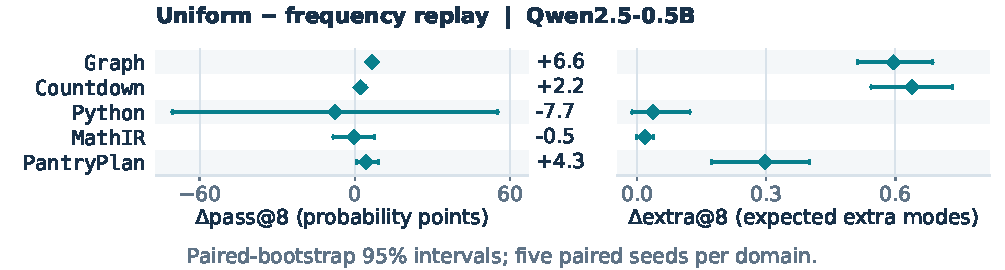
\includegraphics[width=\linewidth]{figures/replay_key_weighting.pdf}
\caption{\textbf{Uniform weighting preserves more verified alternatives.}
Uniform minus frequency-weighted replay at Qwen2.5-0.5B, Level 1, with five matched seeds. Extra modes are $B_8=\texttt{distinct@8}-\texttt{pass@8}$. Bars show nominal 95\% paired-seed bootstrap intervals. The mean gain is $.318$ extra modes, with an inconclusive correctness effect. Extra modes remain coupled to correctness; they do not measure success-conditional \pmd{}.}
\label{fig:replay-key-weighting}
\end{figure}

\clearpage
\section{Fixed Semantic-Entropy Factorials}
\label{app:semantic-current-factorial}
A fixed semantic-entropy bonus can be applied with or without verified replay.
Pantry semantic arms use the registered E85 repairs: original E81/E82/E83
Pantry runs received zero semantic advantage because of an outcome-key defect
and remain excluded. The historical Falcon factorial display had not applied
that repair; no value from its superseded Pantry column is reused here.
The matched four-arm studies compare its effect on Dr.GRPO, its effect on
Re:Dr.GRPO, and the difference of these effects. This restores the full
factorial detail beyond the main semantic-only comparator. We reconstruct
exact terminal four-draw endpoints under the current source-admission policy:
identical repeated metrics are deduplicated, unapproved conflicting retries
abort, and the previously excluded Falcon Countdown replay seed 59 remains
excluded. All three contrasts in that cell therefore use the common four
seeds 55--58; other 0.5B/1B cells use five. No old five-seed Falcon Countdown
interval is reused. Tables report paired seed means and pointwise Student-$t$
95\% intervals, without pooling models or domains.

The Qwen2.5-3B extension has only fixed seed 70 and no semantic-only arm.
Its on-replay comparison is descriptive, has no interval and cannot identify
a factorial interaction. These are fixed-coefficient experiments, not a
sweep over entropy strengths. Their endpoints do not establish that semantic
entropy reproduces the mechanism of a bank that revisits verified keys.
\begin{table}[H]
\centering
\caption{Qwen2.5-0.5B: fixed semantic-entropy effects. Without replay is semantic-only minus Dr.GRPO; on replay is semantic-plus-replay minus Re:Dr.GRPO; interaction subtracts the first effect from the second. Extra modes equal distinct@8 minus pass@8.}
\label{tab:semantic-current-qwen2505b}
\scriptsize
\setlength{\tabcolsep}{3pt}
\begin{tabular}{lr l rrr}
\toprule
Domain & $n$ & Contrast & $\Delta$ pass@8 & $\Delta$ distinct@8 & $\Delta$ extra modes \\
\midrule
Graph & 5 & Without replay & $0.002$ $[-0.028, 0.031]$ & $0.004$ $[-0.034, 0.041]$ & $0.002$ $[-0.010, 0.014]$ \\
Graph & 5 & On replay & $-0.002$ $[-0.027, 0.023]$ & $-0.022$ $[-0.179, 0.135]$ & $-0.020$ $[-0.161, 0.120]$ \\
Graph & 5 & Interaction & $-0.004$ $[-0.035, 0.028]$ & $-0.026$ $[-0.193, 0.141]$ & $-0.022$ $[-0.161, 0.116]$ \\
Countdown & 5 & Without replay & $0.141$ $[-0.047, 0.330]$ & $0.184$ $[0.011, 0.358]$ & $0.043$ $[0.001, 0.085]$ \\
Countdown & 5 & On replay & $-0.003$ $[-0.033, 0.028]$ & $0.115$ $[0.022, 0.209]$ & $0.118$ $[0.004, 0.232]$ \\
Countdown & 5 & Interaction & $-0.144$ $[-0.326, 0.037]$ & $-0.069$ $[-0.233, 0.095]$ & $0.075$ $[-0.051, 0.201]$ \\
Python & 5 & Without replay & $0.000$ $[0.000, 0.000]$ & $0.000$ $[0.000, 0.000]$ & $0.000$ $[0.000, 0.000]$ \\
Python & 5 & On replay & $-0.002$ $[-0.717, 0.714]$ & $0.016$ $[-0.747, 0.780]$ & $0.018$ $[-0.164, 0.200]$ \\
Python & 5 & Interaction & $-0.002$ $[-0.717, 0.714]$ & $0.016$ $[-0.747, 0.780]$ & $0.018$ $[-0.164, 0.200]$ \\
MathIR & 5 & Without replay & $-0.121$ $[-0.349, 0.106]$ & $-0.121$ $[-0.347, 0.105]$ & $0.001$ $[-0.006, 0.008]$ \\
MathIR & 5 & On replay & $0.031$ $[-0.035, 0.097]$ & $0.035$ $[-0.044, 0.114]$ & $0.004$ $[-0.047, 0.055]$ \\
MathIR & 5 & Interaction & $0.153$ $[-0.018, 0.324]$ & $0.156$ $[-0.050, 0.362]$ & $0.003$ $[-0.052, 0.058]$ \\
Pantry & 5 & Without replay & $0.201$ $[0.119, 0.283]$ & $1.120$ $[0.888, 1.352]$ & $0.919$ $[0.713, 1.124]$ \\
Pantry & 5 & On replay & $0.141$ $[0.044, 0.238]$ & $1.095$ $[0.368, 1.823]$ & $0.955$ $[0.321, 1.589]$ \\
Pantry & 5 & Interaction & $-0.061$ $[-0.161, 0.040]$ & $-0.025$ $[-0.826, 0.777]$ & $0.036$ $[-0.682, 0.754]$ \\
\bottomrule
\end{tabular}
\end{table}
\begin{table}[H]
\centering
\caption{Falcon3-1B: fixed semantic-entropy effects. Without replay is semantic-only minus Dr.GRPO; on replay is semantic-plus-replay minus Re:Dr.GRPO; interaction subtracts the first effect from the second. Extra modes equal distinct@8 minus pass@8.}
\label{tab:semantic-current-falcon31b}
\scriptsize
\setlength{\tabcolsep}{3pt}
\begin{tabular}{lr l rrr}
\toprule
Domain & $n$ & Contrast & $\Delta$ pass@8 & $\Delta$ distinct@8 & $\Delta$ extra modes \\
\midrule
Graph & 5 & Without replay & $0.036$ $[-0.192, 0.264]$ & $0.205$ $[-0.483, 0.893]$ & $0.169$ $[-0.292, 0.630]$ \\
Graph & 5 & On replay & $0.001$ $[-0.040, 0.043]$ & $-0.006$ $[-0.113, 0.101]$ & $-0.007$ $[-0.091, 0.077]$ \\
Graph & 5 & Interaction & $-0.035$ $[-0.237, 0.168]$ & $-0.211$ $[-0.886, 0.464]$ & $-0.176$ $[-0.649, 0.297]$ \\
Countdown & 4 & Without replay & $0.004$ $[-0.092, 0.100]$ & $-0.042$ $[-0.258, 0.173]$ & $-0.047$ $[-0.168, 0.074]$ \\
Countdown & 4 & On replay & $0.036$ $[-0.028, 0.101]$ & $0.047$ $[-0.082, 0.177]$ & $0.011$ $[-0.064, 0.087]$ \\
Countdown & 4 & Interaction & $0.032$ $[-0.098, 0.161]$ & $0.090$ $[-0.188, 0.367]$ & $0.058$ $[-0.099, 0.216]$ \\
Python & 5 & Without replay & $0.002$ $[-0.003, 0.008]$ & $0.002$ $[-0.003, 0.008]$ & $0.000$ $[0.000, 0.000]$ \\
Python & 5 & On replay & $-0.133$ $[-0.308, 0.043]$ & $-0.091$ $[-0.503, 0.321]$ & $0.042$ $[-0.296, 0.380]$ \\
Python & 5 & Interaction & $-0.135$ $[-0.310, 0.040]$ & $-0.093$ $[-0.507, 0.321]$ & $0.042$ $[-0.296, 0.380]$ \\
MathIR & 5 & Without replay & $-0.002$ $[-0.063, 0.060]$ & $-0.002$ $[-0.063, 0.060]$ & $0.000$ $[0.000, 0.000]$ \\
MathIR & 5 & On replay & $0.086$ $[0.004, 0.168]$ & $0.108$ $[0.003, 0.214]$ & $0.022$ $[-0.009, 0.054]$ \\
MathIR & 5 & Interaction & $0.087$ $[0.029, 0.146]$ & $0.110$ $[0.043, 0.176]$ & $0.022$ $[-0.009, 0.054]$ \\
Pantry & 5 & Without replay & $0.011$ $[-0.019, 0.041]$ & $0.091$ $[-0.161, 0.342]$ & $0.080$ $[-0.142, 0.301]$ \\
Pantry & 5 & On replay & $0.025$ $[-0.044, 0.094]$ & $0.382$ $[-0.702, 1.465]$ & $0.356$ $[-0.670, 1.382]$ \\
Pantry & 5 & Interaction & $0.014$ $[-0.052, 0.081]$ & $0.291$ $[-0.646, 1.228]$ & $0.277$ $[-0.615, 1.168]$ \\
\bottomrule
\end{tabular}
\end{table}
\begin{table}[H]
\centering
\caption{Qwen2.5-3B: fixed semantic-entropy effects. Without replay is semantic-only minus Dr.GRPO; on replay is semantic-plus-replay minus Re:Dr.GRPO; interaction subtracts the first effect from the second. Extra modes equal distinct@8 minus pass@8.}
\label{tab:semantic-current-qwen253b}
\scriptsize
\setlength{\tabcolsep}{3pt}
\begin{tabular}{lr l rrr}
\toprule
Domain & $n$ & Contrast & $\Delta$ pass@8 & $\Delta$ distinct@8 & $\Delta$ extra modes \\
\midrule
Graph & 1 & On replay & $-0.016$ & $-0.010$ & $0.006$ \\
Countdown & 1 & On replay & $0.039$ & $0.146$ & $0.107$ \\
Python & 1 & On replay & $-0.590$ & $-1.215$ & $-0.625$ \\
MathIR & 1 & On replay & $0.033$ & $0.010$ & $-0.023$ \\
Pantry & 1 & On replay & $0.035$ & $0.393$ & $0.357$ \\
\bottomrule
\end{tabular}
\end{table}
\path{results/semantic_current_summary_20260912.json} retains per-seed
endpoints, source hashes, exclusion evidence and all three metrics.
\path{ops/build_paper_semantic_current_summary.py} reconstructs these contrasts
with the same strict endpoint reader used by the current core comparison, including all documented exclusions.


\newpage
\section{Concentration and Replay Mechanisms}
\label{app:ablations}

\subsection{Concentration with 64 responses per prompt}
\label{app:fresh-concentration}

We evaluate initial and terminal checkpoints on the 128 held-out Level-1
\texttt{Graph} and \texttt{PantryPlan} prompts, drawing 64 responses per
prompt from new sampling streams. This evaluation is separate from the
32-response comparison in Fig.~\ref{fig:concentration-story}. It covers
Qwen2.5-0.5B, Falcon3-1B, and Qwen2.5-3B, with five training seeds for
Dr.GRPO, Re:Dr, MaxRL, and Re:Max. For each model, the five initial
evaluations use independent sampling from the same weights. Each initial
evaluation is paired with one training seed and shared across the four methods.

\paragraph{Matched comparisons.}
We estimate \pmd{} from correct-output pairs and average promptwise
differences over prompts with at least two correct responses in both
conditions, then average the five seed effects equally. Thus positive
changes indicate more diverse correct modes. Matching prompts within each
comparison differs from subtracting means over separately eligible prompts.
The eligible population ranges from 37 to 127 of the 128 prompts across
comparisons and seeds. Effects from different comparisons therefore cannot
be subtracted to reconstruct a trajectory on a common prompt population. Tables~\ref{tab:fresh-concentration-initial}
and~\ref{tab:fresh-concentration-replay} give all 36 contrasts and their
eligible-prompt ranges. Intervals are nominal 95\% paired Student-$t$
intervals with four degrees of freedom. They describe variation over the
five training-seed and initial-sampling pairs, conditional on the fixed
prompts and initial weights. They are unadjusted for multiple comparisons
and do not quantify uncertainty over unseen tasks.

\begin{figure}[t]
 \centering
 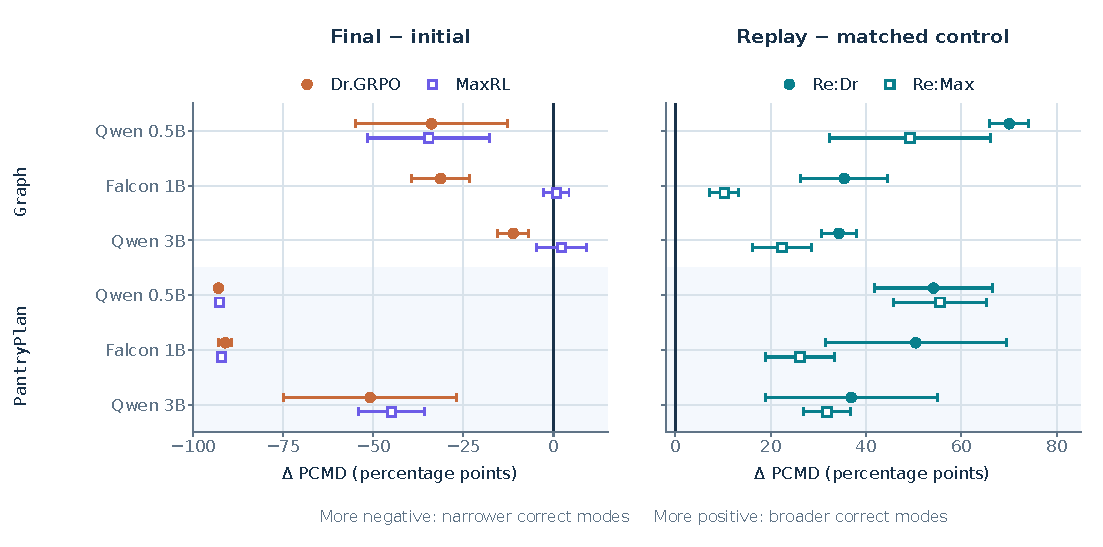
\includegraphics[width=\linewidth]{figures/fresh_concentration_pcmd_20260912.pdf}
 \caption{\textbf{Replay increases correct-mode diversity at a 64-response budget.}
 Left: Dr.GRPO reduces \pmd{} in all six model--domain comparisons;
 MaxRL's change is inconclusive for Falcon3-1B and Qwen2.5-3B \texttt{Graph}.
 Right: replay increases \pmd{} in all twelve comparisons with matched
 trained controls. Points show means over five paired seeds; bars give
 nominal 95\% Student-$t$ intervals. Each contrast uses its own jointly
 eligible Level-1 prompts. Horizontal scales differ between panels.}
 \label{fig:fresh-concentration}
\end{figure}

\paragraph{Concentration and mitigation.}
Dr.GRPO reduces \pmd{} in all six model--domain comparisons and all
30 seed effects. Replay increases \pmd{} relative to its matched trained
control under both objectives in all twelve comparisons and all 60 seed
effects. All eighteen nominal intervals exclude zero
(Fig.~\ref{fig:fresh-concentration}). These directions also hold when
pooling correct pairs, using each policy's own eligible prompts, or
restricting to the intersection of eligible prompts across seeds.
The intersection can be small: for Qwen2.5-0.5B \texttt{Graph}, only five
prompts are jointly eligible across all seeds in comparisons involving Dr.GRPO.

MaxRL alone does not consistently reduce diversity: its Falcon3-1B and
Qwen2.5-3B \texttt{Graph} intervals include zero. An improvement over a
trained control also need not restore initial diversity. Both replay
variants remain below initial \pmd{} in \texttt{PantryPlan} at every
scale, whereas their \texttt{Graph} comparisons exceed the initial value.
These results describe diversity within each comparison's eligible prompt
population; they do not establish recovery of the same individual modes.

\paragraph{Correctness, coverage, and sampling budget.}
All 24 trained-versus-initial comparisons increase per-response
correctness averaged over all evaluation prompts, in every seed. Nevertheless, every
\texttt{PantryPlan} method--scale comparison has lower \texttt{pass@64}
than initialization in every seed. Averaging over all evaluation prompts,
replay improves mean
\texttt{pass@8}, \texttt{distinct@8}, \texttt{pass@64}, and
\texttt{distinct@64} relative to its trained control in all twelve
comparisons; per-response correctness improves in seven of twelve.
On jointly eligible prompts, however, replay lowers mean correctness in
eleven of twelve comparisons. The concentration effects therefore do not
hold correctness fixed.

The eight-response metrics average over subsets of eight responses from
each 64-response pool (rarefaction). For Qwen2.5-3B \texttt{Graph}, Dr.GRPO increases per-response correctness by
14.49 percentage points and \texttt{distinct@8} by 0.112 modes per prompt,
while reducing \pmd{} by 11.20 points and \texttt{distinct@64} by
0.220 modes. The change in verified-mode count reverses sign between
eight and 64 responses in every seed. A gain at one sampling budget thus
need not persist at a larger budget. These evaluations measure the
distribution of correct responses and the modes observed in finite samples;
they do not establish exact mode extinction, recovery of the full support,
or a causal effect of diversity on accuracy.

% Generated by ops/build_paper_fresh_concentration.py; do not hand edit.
\begin{table}[t]
\centering
\small
\setlength{\tabcolsep}{4pt}
\caption{64-response evaluation: trained policy minus initialization. Changes in \pmd{} are in probability units; positive values indicate more diverse correct modes. Brackets give nominal 95\% paired Student-$t$ intervals ($n=5$, four degrees of freedom). The last column gives the range of jointly eligible prompts across seeds, out of 128. Each row uses its own matched prompt population.}
\label{tab:fresh-concentration-initial}
\begin{tabular}{llrr}
\toprule
Domain & Contrast & $\Delta\pmd$ [95\% interval] & Joint prompts \\
\midrule
\multicolumn{4}{l}{\textbf{Qwen2.5-0.5B}} \\
\texttt{Graph} & Dr.GRPO $-$ initial & $-0.338\;[-0.550, -0.126]$ & 37--45 \\
 & Re:Dr $-$ initial & $+0.217\;[+0.190, +0.243]$ & 97--103 \\
 & MaxRL $-$ initial & $-0.346\;[-0.516, -0.177]$ & 37--86 \\
 & Re:Max $-$ initial & $+0.155\;[+0.107, +0.203]$ & 97--101 \\
\texttt{PantryPlan} & Dr.GRPO $-$ initial & $-0.929\;[-0.936, -0.923]$ & 62--68 \\
 & Re:Dr $-$ initial & $-0.357\;[-0.445, -0.269]$ & 109--122 \\
 & MaxRL $-$ initial & $-0.927\;[-0.932, -0.921]$ & 62--71 \\
 & Re:Max $-$ initial & $-0.355\;[-0.438, -0.272]$ & 108--124 \\
\midrule
\multicolumn{4}{l}{\textbf{Falcon3-1B}} \\
\texttt{Graph} & Dr.GRPO $-$ initial & $-0.313\;[-0.393, -0.233]$ & 75--99 \\
 & Re:Dr $-$ initial & $+0.043\;[+0.006, +0.081]$ & 100--107 \\
 & MaxRL $-$ initial & $+0.008\;[-0.027, +0.043]$ & 104--109 \\
 & Re:Max $-$ initial & $+0.119\;[+0.096, +0.141]$ & 106--109 \\
\texttt{PantryPlan} & Dr.GRPO $-$ initial & $-0.910\;[-0.928, -0.893]$ & 81--86 \\
 & Re:Dr $-$ initial & $-0.378\;[-0.507, -0.250]$ & 104--110 \\
 & MaxRL $-$ initial & $-0.921\;[-0.925, -0.916]$ & 81 \\
 & Re:Max $-$ initial & $-0.519\;[-0.575, -0.462]$ & 106--116 \\
\midrule
\multicolumn{4}{l}{\textbf{Qwen2.5-3B}} \\
\texttt{Graph} & Dr.GRPO $-$ initial & $-0.112\;[-0.156, -0.069]$ & 78--86 \\
 & Re:Dr $-$ initial & $+0.226\;[+0.212, +0.240]$ & 88--96 \\
 & MaxRL $-$ initial & $+0.022\;[-0.048, +0.092]$ & 81--93 \\
 & Re:Max $-$ initial & $+0.254\;[+0.234, +0.274]$ & 90--96 \\
\texttt{PantryPlan} & Dr.GRPO $-$ initial & $-0.509\;[-0.750, -0.268]$ & 69--99 \\
 & Re:Dr $-$ initial & $-0.115\;[-0.157, -0.073]$ & 101--110 \\
 & MaxRL $-$ initial & $-0.449\;[-0.541, -0.358]$ & 83--98 \\
 & Re:Max $-$ initial & $-0.116\;[-0.208, -0.024]$ & 105--110 \\
\bottomrule
\end{tabular}
\end{table}

% Generated by ops/build_paper_fresh_concentration.py; do not hand edit.
\begin{table}[t]
\centering
\small
\setlength{\tabcolsep}{4pt}
\caption{64-response evaluation: replay minus its matched trained control. Changes in \pmd{} are in probability units; positive values indicate more diverse correct modes. Brackets give nominal 95\% paired Student-$t$ intervals ($n=5$, four degrees of freedom). The last column gives the range of jointly eligible prompts across seeds, out of 128. Each row uses its own matched prompt population.}
\label{tab:fresh-concentration-replay}
\begin{tabular}{llrr}
\toprule
Domain & Contrast & $\Delta\pmd$ [95\% interval] & Joint prompts \\
\midrule
\multicolumn{4}{l}{\textbf{Qwen2.5-0.5B}} \\
\texttt{Graph} & Re:Dr $-$ Dr.GRPO & $+0.700\;[+0.659, +0.742]$ & 40--46 \\
 & Re:Max $-$ MaxRL & $+0.493\;[+0.324, +0.662]$ & 41--107 \\
\texttt{PantryPlan} & Re:Dr $-$ Dr.GRPO & $+0.542\;[+0.418, +0.665]$ & 62--68 \\
 & Re:Max $-$ MaxRL & $+0.555\;[+0.458, +0.652]$ & 61--71 \\
\midrule
\multicolumn{4}{l}{\textbf{Falcon3-1B}} \\
\texttt{Graph} & Re:Dr $-$ Dr.GRPO & $+0.354\;[+0.264, +0.445]$ & 73--101 \\
 & Re:Max $-$ MaxRL & $+0.103\;[+0.072, +0.133]$ & 122--127 \\
\texttt{PantryPlan} & Re:Dr $-$ Dr.GRPO & $+0.505\;[+0.315, +0.694]$ & 80--84 \\
 & Re:Max $-$ MaxRL & $+0.262\;[+0.190, +0.334]$ & 81 \\
\midrule
\multicolumn{4}{l}{\textbf{Qwen2.5-3B}} \\
\texttt{Graph} & Re:Dr $-$ Dr.GRPO & $+0.343\;[+0.307, +0.380]$ & 94--107 \\
 & Re:Max $-$ MaxRL & $+0.224\;[+0.163, +0.286]$ & 105--123 \\
\texttt{PantryPlan} & Re:Dr $-$ Dr.GRPO & $+0.369\;[+0.188, +0.550]$ & 72--101 \\
 & Re:Max $-$ MaxRL & $+0.319\;[+0.270, +0.367]$ & 89--99 \\
\bottomrule
\end{tabular}
\end{table}

\FloatBarrier


\subsection{Conditional concentration from saved training outputs}
\label{app:conditional-concentration}

This retrospective analysis distinguishes the distribution of correct keys
from the probability of producing a correct output. If $P=0$, $C$ is undefined
and $B_2=0$. For a fixed prompt with
correct mass $P>0$, write $q_c=\Pr[V(Y,s_x)=c\mid V(Y,s_x)\ne\bot]$ and define
\begin{equation}
 C(q)=\sum_c q_c^2,\qquad B_2=2P-P^2C(q).
 \label{eq:collision-breadth-bridge}
\end{equation}
The first quantity is the probability that two independent correct outputs
share a key. The second identity follows by expanding
$B_2=\sum_c[1-(1-Pq_c)^2]$. It makes explicit why sampled breadth can
change through correctness or conditional concentration. A decrease in $C$
alone does not imply majorization, larger total support, or recovery of any
particular mode. In particular, observed collisions cannot establish that
an unobserved key has exactly zero probability under the policy.

\paragraph{Connection to the conditional theory.}
Under the assumptions of Theorem~\ref{thm:grpo-collapse}, the time change in
its proof gives $dq_c/d\tau=q_c(q_c-C)$. Consequently,
\begin{equation}
 \frac{dC}{d\tau}
 =2\left(\sum_c q_c^3-C^2\right)
 =2\operatorname{Var}_{c\sim q}(q_c)\ge0.
 \label{eq:collision-flow}
\end{equation}
The variance vanishes exactly when $q$ is uniform on its positive support.
Thus concentration is monotone along this ideal categorical flow, with
strict increase whenever the positive coordinates are unequal. The identity
provides a theoretical basis for the diagnostic; it does not establish
monotonicity for the implemented neural optimizer or a corresponding
monotonic decrease under finite-bank replay.

\paragraph{Estimator and identifiable population.}
The pair statistic is the one defined in App.~\ref{app:metric-sampling}, read
here in the collision orientation, $\widehat C=1-\widehat{\pmd}$, over a prompt's
$R\ge2$ correct samples: the contrast this analysis reports is about
concentration, so the orientation that rises with it is the one to print. Its
promptwise unbiasedness, and the limits of that identity under joint selection,
are established there. We leave $R<2$ undefined, rather than assigning a
concentration value to insufficient correct observations.

For each paired training seed $s$, let $E_s$ contain exactly the prompts with
a defined estimate in both conditions. The reported seed contrast is
$|E_s|^{-1}\sum_{x\in E_s}(\widehat C_{B,x}-\widehat C_{A,x})$ when
$E_s$ is nonempty. We then weight defined training seeds equally, preserving
all registered blocks and their missingness. Before/after contrasts use each
method's own initial checkpoint and step 3,072; replay contrasts compare
matched terminal conditions. No other method substitutes for a missing
initial evaluation. Five defined seeds receive nominal Student-$t$ intervals;
partial blocks are descriptive. These intervals describe the measured seed
means and are not simultaneous guarantees or uncertainty over unseen prompts.

The hosted analysis uses the same promptwise collision concept but pools
correct pairs. At a common sampling budget, the ratio of expected colliding
and correct pair counts is
$\sum_x P_x^2 C(q_x)/\sum_x P_x^2$. Its finite-sample ratio is not generally
unbiased for that target. The training contrast here weights eligible prompts
equally. Changing correctness can change either eligibility or hosted pair
weights, so the two aggregate values are not directly interchangeable.

\paragraph{Retrospective protocol and source coverage.}
The estimator and comparisons were recorded before the initial concentration
contrasts, with the sampling-stream amendment also preceding those effects.
Two retrospective extensions then followed the paper's completed source
census. The first included thirteen newly available terminal checkpoints
and withdrew one conflicted initial checkpoint. The September~12 extension
adds all ten remaining Level-2 Pantry terminal checkpoints, reusing 752
unchanged checkpoint identities and changing no estimator or eligibility
rule. All prior results, caches, and source snapshots remain preserved.
The final collection contains 475 registered runs and 902 available
checkpoint evaluations, with 74 Dr.GRPO and 75 MaxRL Level-1 replay pairs
and 25 pairs per objective at Level~2 before conditional eligibility.
Complete terminal coverage neither supplies missing initial outputs nor
makes every conditional contrast identifiable. Exact source hashes and
both retrospective extensions' timing remain bound to the result artifact.

\paragraph{Sampling-stream audit.}
Four saved eight-output groups do not provide 32 independently seeded
responses. The recorded parent seeds increment by one; the audited vLLM V0
sampler increments each child's seed by its output index. The resulting
nominal stream ranges overlap, giving eleven distinct identifiers. For each
prompt and checkpoint we retain the earliest draw/output position for every
identifier, independently of correctness or key identity. Repeated positions
sometimes disagree, so identical seed integers are not treated as a proof of
identical outputs. Archived actor source is available for 150 of the 400
factorial cells and none of the 75 additional GRPO cells; historical dependency
identity is not cryptographically established for every run. The stream
mapping rests on the audited implementation and recorded neutral request
contract, with the historical-runtime assumption stated explicitly.

The primary eleven-stream comparisons reuse nominal streams across conditions
and remain descriptive after common eligibility. Two additional orientations
compare the lower five identifiers in condition A with the upper six in B,
then reverse the assignment. Each orientation retains its own eligible prompts
and seed counts. Shared identifiers also recur across prompts; neither their
separation across conditions nor these selected-population means establishes
independent prompt observations. Independent fixed-law sampling is an explicit
assumption of the estimator identity, not a conclusion of the source audit.

Original \texttt{mean@8}, \texttt{pass@8}, and \texttt{distinct@8} remain averages
over the four intact groups, reconstructed from all saved verified keys.
Cross-group overlap affects dependence, not linearity of those marginal
averages. The complete result artifact also retains each intact-group
collision comparison, a fixed-first-group check, fixed-across-seed prompt
intersections, and four-condition change differences. A naive concatenated
32-position collision is retained solely as a reuse diagnostic. These views
are not treated as independent replications or substituted for missing cells.

\paragraph{Findings and their limits.}
In Graph and PantryPlan, all twelve Dr.GRPO/GRPO before/after comparisons
across the three scales show increased conditional concentration, with
nominal intervals above zero. Correctness also increases on those same
eligible prompts. Graph's increases range from $.098$ to $.274$; PantryPlan's
range from $.447$ to $.887$. The two disjoint orientations agree in direction
in eleven of these twelve blocks; Falcon Graph with GRPO is the exception.
The evidence therefore supports observed training-induced concentration in
these tasks, with a visible sampling sensitivity, rather than a universal
claim about every RLVR run or exact disappearance of modes.

Re:Dr lowers concentration relative to Dr.GRPO in all six Graph and
PantryPlan comparisons: changes range from $-.756$ to $-.273$ in Graph and
$-.433$ to $-.300$ in PantryPlan. Both disjoint orientations agree in direction
in all six, and their primary nominal intervals lie below zero. These
comparisons also have lower per-sample correctness on their jointly eligible
prompts. They establish a change in the conditional correct-key distribution
on that observable population; they do not hold correctness fixed or imply
that every accuracy measure improves on the same prompts. Full-test
\texttt{pass@8} and sampled breadth remain the separately reported primary
outcomes of the replay experiment.

The other domains constrain the interpretation. Dr.GRPO/GRPO Python initial
outputs provide no jointly eligible prompts at this budget, so their
longitudinal collision contrast is unidentified. Some Countdown initial
comparisons use only one or two eligible prompts per seed. Several MathIR
conditions already have observed collision one, leaving little detectable
change. MaxRL comparisons, incomplete saved-output cohorts, and the two
sampling orientations are reported explicitly in the following tables;
we do not infer a universal concentration benefit from raw breadth gains.

In the completed 3B MaxRL replay cohort, Countdown, Python, and PantryPlan
show lower concentration with nominal intervals below zero; MathIR's measured
contrast is zero. Graph's primary contrast is negative, but its two disjoint
orientations disagree in direction, as they do for Falcon Graph with MaxRL.
At Level 2, both Graph replay contrasts are negative with agreement across
orientations. Complete PantryPlan training still leaves sparse conditional
populations: Re:Dr has a defined collision contrast for three seeds
(2--16 eligible prompts), with mean $+.495$; Re:Max has four defined
seeds (1--19 eligible prompts), with mean $+.439$. Their disjoint-orientation
means are also positive but retain fewer defined seeds. Neither contrast
receives a five-seed interval. Thus the full endpoint breadth gains coexist
with increased concentration on these small jointly correct subsets; they
do not establish uniformly reduced conditional concentration.

% Generated by ops/exp_scaling/build_paper_conditional_concentration_appendix.py.
\begin{table}[!htbp]
\centering
\scriptsize
\setlength{\tabcolsep}{3pt}
\begin{tabular}{@{}llcrlrrr@{}}
\toprule
Domain & Objective & $n$ & $\Delta\widehat C$ & nominal 95\% interval & $|E_s|$ & split 0 ($n$) & split 1 ($n$) \\
\midrule
\texttt{Graph} & Dr.GRPO & 5 & +0.242 & [+0.110, +0.373] & 17--40 & +0.257 (5) & +0.284 (5) \\
\texttt{Graph} & GRPO & 5 & +0.221 & [+0.097, +0.344] & 15--28 & +0.268 (5) & +0.287 (5) \\
\texttt{Graph} & MaxRL & 5 & +0.145 & [-0.033, +0.324] & 18--40 & +0.115 (5) & +0.174 (5) \\
\texttt{Graph} & Re:Dr & 5 & -0.507 & [-0.558, -0.456] & 45--49 & -0.519 (5) & -0.465 (5) \\
\texttt{Graph} & Re:Max & 5 & -0.399 & [-0.458, -0.339] & 40--51 & -0.436 (5) & -0.348 (5) \\
\texttt{Countdown} & Dr.GRPO & 5 & +1.000 & [+1.000, +1.000] & 1--2 & -- (0) & +1.000 (5) \\
\texttt{Countdown} & GRPO & 5 & +0.964 & [+0.863, +1.065] & 1--2 & -- (0) & +0.920 (5) \\
\texttt{Countdown} & MaxRL & 4 & +0.977 & -- & 0--2 & -- (0) & +1.000 (4) \\
\texttt{Countdown} & Re:Dr & 5 & +0.467 & [+0.117, +0.816] & 1--3 & -- (0) & +0.713 (4) \\
\texttt{Countdown} & Re:Max & 5 & +0.420 & [+0.359, +0.480] & 1--2 & -- (0) & +0.493 (5) \\
\texttt{Python} & Dr.GRPO & 0 & -- & -- & 0 & -- (0) & -- (0) \\
\texttt{Python} & GRPO & 0 & -- & -- & 0 & -- (0) & -- (0) \\
\texttt{Python} & MaxRL & 0 & -- & -- & 0 & -- (0) & -- (0) \\
\texttt{Python} & Re:Dr & 0 & -- & -- & 0 & -- (0) & -- (0) \\
\texttt{Python} & Re:Max & 0 & -- & -- & 0 & -- (0) & -- (0) \\
\texttt{MathIR} & Dr.GRPO & 5 & +0.000 & [+0.000, +0.000] & 5--8 & +0.000 (5) & +0.000 (1) \\
\texttt{MathIR} & GRPO & 5 & +0.040 & [-0.071, +0.151] & 4--10 & +0.000 (5) & +0.250 (2) \\
\texttt{MathIR} & MaxRL & 5 & +0.022 & [-0.039, +0.084] & 5--9 & +0.000 (5) & +0.067 (5) \\
\texttt{MathIR} & Re:Dr & 5 & +0.059 & [-0.046, +0.163] & 8--11 & +0.000 (5) & +0.367 (2) \\
\texttt{MathIR} & Re:Max & 5 & +0.063 & [-0.009, +0.134] & 9--11 & +0.000 (5) & +0.250 (5) \\
\texttt{PantryPlan} & Dr.GRPO & 5 & +0.833 & [+0.819, +0.847] & 54--64 & +1.000 (5) & +1.000 (5) \\
\texttt{PantryPlan} & GRPO & 5 & +0.849 & [+0.845, +0.853] & 64--65 & +1.000 (5) & +1.000 (5) \\
\texttt{PantryPlan} & MaxRL & 5 & +0.859 & [+0.836, +0.881] & 54--65 & +1.000 (5) & +1.000 (5) \\
\texttt{PantryPlan} & Re:Dr & 5 & +0.413 & [+0.345, +0.481] & 78--89 & +0.543 (5) & +0.538 (5) \\
\texttt{PantryPlan} & Re:Max & 5 & +0.446 & [+0.324, +0.567] & 80--88 & +0.593 (5) & +0.550 (5) \\
\bottomrule
\end{tabular}
\caption{\textbf{Initial-to-final conditional concentration: Qwen2.5-0.5B, Level 1.} Each row compares the same method at initialization and step 3,072; positive $\Delta\widehat C$ means greater concentration among correct outputs. $n$ counts seeds with defined estimates; $|E_s|$ gives the range of eligible prompt counts. Splits 0 and 1 reverse the assignment of disjoint stream identifiers, with eligibility determined separately. Nominal 95\% Student-$t$ intervals require five defined seed estimates.}
\end{table}

\begin{table}[!htbp]
\centering
\scriptsize
\setlength{\tabcolsep}{3pt}
\begin{tabular}{@{}llcrlrrr@{}}
\toprule
Domain & Objective & $n$ & $\Delta\widehat C$ & nominal 95\% interval & $|E_s|$ & split 0 ($n$) & split 1 ($n$) \\
\midrule
\texttt{Graph} & Dr.GRPO & 5 & +0.233 & [+0.124, +0.343] & 41--54 & +0.059 (5) & +0.428 (5) \\
\texttt{Graph} & GRPO & 5 & +0.098 & [+0.026, +0.170] & 48--56 & -0.186 (5) & +0.273 (5) \\
\texttt{Graph} & MaxRL & 3 & -0.113 & -- & 48--52 & -0.083 (3) & +0.039 (3) \\
\texttt{Graph} & Re:Dr & 5 & -0.007 & [-0.065, +0.050] & 37--45 & +0.048 (5) & +0.045 (5) \\
\texttt{Graph} & Re:Max & 2 & -0.062 & -- & 51--52 & -0.300 (2) & -0.015 (2) \\
\texttt{Countdown} & Dr.GRPO & 5 & +0.022 & [-0.038, +0.082] & 6--8 & +0.000 (5) & -- (0) \\
\texttt{Countdown} & GRPO & 5 & +0.180 & [+0.128, +0.231] & 6--11 & +0.126 (5) & -- (0) \\
\texttt{Countdown} & MaxRL & 2 & +0.182 & -- & 11 & +0.143 (2) & -- (0) \\
\texttt{Countdown} & Re:Dr & 4 & +0.035 & -- & 10--11 & +0.158 (4) & -- (0) \\
\texttt{Countdown} & Re:Max & 1 & +0.135 & -- & 11 & +0.143 (1) & -- (0) \\
\texttt{Python} & Dr.GRPO & 0 & -- & -- & 0 & -- (0) & -- (0) \\
\texttt{Python} & GRPO & 0 & -- & -- & 0 & -- (0) & -- (0) \\
\texttt{Python} & MaxRL & 0 & -- & -- & 0 & -- (0) & -- (0) \\
\texttt{Python} & Re:Dr & 0 & -- & -- & 0 & -- (0) & -- (0) \\
\texttt{Python} & Re:Max & 0 & -- & -- & -- & -- (0) & -- (0) \\
\texttt{MathIR} & Dr.GRPO & 5 & +0.105 & [+0.088, +0.122] & 6 & -- (0) & +0.098 (5) \\
\texttt{MathIR} & GRPO & 5 & +0.054 & [-0.099, +0.206] & 3--7 & -- (0) & +0.233 (5) \\
\texttt{MathIR} & MaxRL & 1 & +0.278 & -- & 6 & +1.000 (1) & +0.133 (1) \\
\texttt{MathIR} & Re:Dr & 5 & +0.086 & [+0.026, +0.146] & 6--7 & -- (0) & +0.111 (5) \\
\texttt{MathIR} & Re:Max & 2 & +0.167 & -- & 5--6 & +1.000 (2) & +0.000 (2) \\
\texttt{PantryPlan} & Dr.GRPO & 5 & +0.886 & [+0.886, +0.886] & 76 & +1.000 (5) & +1.000 (5) \\
\texttt{PantryPlan} & GRPO & 5 & +0.863 & [+0.798, +0.928] & 76 & +0.945 (5) & +1.000 (5) \\
\texttt{PantryPlan} & MaxRL & 1 & +0.886 & -- & 76 & +1.000 (1) & +1.000 (1) \\
\texttt{PantryPlan} & Re:Dr & 4 & +0.437 & -- & 75--83 & +0.451 (4) & +0.618 (4) \\
\texttt{PantryPlan} & Re:Max & 2 & +0.746 & -- & 76--78 & +0.740 (2) & +0.978 (2) \\
\bottomrule
\end{tabular}
\caption{\textbf{Initial-to-final conditional concentration: Falcon3-1B, Level 1.} Each row compares the same method at initialization and step 3,072; positive $\Delta\widehat C$ means greater concentration among correct outputs. $n$ counts seeds with defined estimates; $|E_s|$ gives the range of eligible prompt counts. Splits 0 and 1 reverse the assignment of disjoint stream identifiers, with eligibility determined separately. Nominal 95\% Student-$t$ intervals require five defined seed estimates.}
\end{table}

\begin{table}[!htbp]
\centering
\scriptsize
\setlength{\tabcolsep}{3pt}
\begin{tabular}{@{}llcrlrrr@{}}
\toprule
Domain & Objective & $n$ & $\Delta\widehat C$ & nominal 95\% interval & $|E_s|$ & split 0 ($n$) & split 1 ($n$) \\
\midrule
\texttt{Graph} & Dr.GRPO & 5 & +0.274 & [+0.232, +0.316] & 44--47 & +0.030 (5) & +0.339 (5) \\
\texttt{Graph} & GRPO & 5 & +0.274 & [+0.207, +0.341] & 46--49 & +0.046 (5) & +0.364 (5) \\
\texttt{Graph} & MaxRL & 5 & +0.072 & [-0.002, +0.145] & 45--55 & -0.208 (5) & +0.215 (5) \\
\texttt{Graph} & Re:Dr & 5 & -0.038 & [-0.060, -0.016] & 48--53 & -0.227 (5) & +0.121 (5) \\
\texttt{Graph} & Re:Max & 5 & -0.145 & [-0.198, -0.093] & 46--52 & -0.220 (5) & +0.165 (5) \\
\texttt{Countdown} & Dr.GRPO & 5 & +0.160 & [+0.109, +0.211] & 11--12 & +0.200 (5) & -0.016 (5) \\
\texttt{Countdown} & GRPO & 5 & +0.182 & [+0.182, +0.182] & 11 & +0.200 (5) & +0.000 (5) \\
\texttt{Countdown} & MaxRL & 5 & +0.056 & [-0.046, +0.159] & 9--11 & +0.050 (5) & +0.000 (5) \\
\texttt{Countdown} & Re:Dr & 5 & +0.020 & [-0.060, +0.099] & 11--15 & +0.169 (5) & -0.071 (5) \\
\texttt{Countdown} & Re:Max & 5 & -0.100 & [-0.145, -0.055] & 10--12 & +0.000 (5) & -0.050 (5) \\
\texttt{Python} & Dr.GRPO & 0 & -- & -- & 0 & -- (0) & -- (0) \\
\texttt{Python} & GRPO & 0 & -- & -- & 0 & -- (0) & -- (0) \\
\texttt{Python} & MaxRL & 5 & +0.000 & [+0.000, +0.000] & 2--9 & +0.000 (2) & +0.000 (5) \\
\texttt{Python} & Re:Dr & 0 & -- & -- & 0 & -- (0) & -- (0) \\
\texttt{Python} & Re:Max & 5 & -0.023 & [-0.050, +0.003] & 9 & +0.000 (5) & -0.040 (5) \\
\texttt{MathIR} & Dr.GRPO & 5 & +0.000 & [+0.000, +0.000] & 11--14 & +0.000 (5) & +0.000 (5) \\
\texttt{MathIR} & GRPO & 5 & +0.000 & [+0.000, +0.000] & 9--11 & +0.000 (5) & +0.000 (5) \\
\texttt{MathIR} & MaxRL & 5 & +0.000 & [+0.000, +0.000] & 7--14 & +0.000 (5) & +0.000 (5) \\
\texttt{MathIR} & Re:Dr & 4 & -0.012 & -- & 14 & +0.000 (4) & +0.000 (4) \\
\texttt{MathIR} & Re:Max & 5 & +0.000 & [+0.000, +0.000] & 12--15 & +0.000 (5) & +0.000 (5) \\
\texttt{PantryPlan} & Dr.GRPO & 5 & +0.447 & [+0.266, +0.627] & 49--67 & +0.478 (5) & +0.245 (5) \\
\texttt{PantryPlan} & GRPO & 5 & +0.469 & [+0.411, +0.526] & 49--62 & +0.514 (5) & +0.271 (5) \\
\texttt{PantryPlan} & MaxRL & 5 & +0.431 & [+0.297, +0.565] & 59--69 & +0.394 (5) & +0.246 (5) \\
\texttt{PantryPlan} & Re:Dr & 5 & +0.184 & [+0.081, +0.288] & 64--71 & +0.087 (5) & +0.037 (5) \\
\texttt{PantryPlan} & Re:Max & 5 & +0.142 & [+0.018, +0.266] & 68--75 & +0.046 (5) & -0.015 (5) \\
\bottomrule
\end{tabular}
\caption{\textbf{Initial-to-final conditional concentration: Qwen2.5-3B, Level 1.} Each row compares the same method at initialization and step 3,072; positive $\Delta\widehat C$ means greater concentration among correct outputs. $n$ counts seeds with defined estimates; $|E_s|$ gives the range of eligible prompt counts. Splits 0 and 1 reverse the assignment of disjoint stream identifiers, with eligibility determined separately. Nominal 95\% Student-$t$ intervals require five defined seed estimates.}
\end{table}

\begin{table}[!htbp]
\centering
\scriptsize
\setlength{\tabcolsep}{3pt}
\begin{tabular}{@{}llcrlrrr@{}}
\toprule
Domain & Objective & $n$ & $\Delta\widehat C$ & nominal 95\% interval & $|E_s|$ & split 0 ($n$) & split 1 ($n$) \\
\midrule
\texttt{Graph} & Dr.GRPO & 5 & +0.625 & [+0.295, +0.955] & 2--10 & +0.633 (2) & +0.860 (5) \\
\texttt{Graph} & MaxRL & 5 & +0.452 & [+0.387, +0.518] & 6--10 & +0.767 (4) & +0.484 (5) \\
\texttt{Graph} & Re:Dr & 5 & -0.204 & [-0.282, -0.126] & 9--11 & +0.033 (5) & -0.372 (5) \\
\texttt{Graph} & Re:Max & 5 & -0.128 & [-0.262, +0.006] & 9--11 & +0.333 (5) & -0.267 (5) \\
\texttt{Countdown} & Dr.GRPO & 1 & +0.000 & -- & 0--1 & -- (0) & -- (0) \\
\texttt{Countdown} & MaxRL & 1 & +0.000 & -- & 0--1 & -- (0) & -- (0) \\
\texttt{Countdown} & Re:Dr & 5 & +0.000 & [+0.000, +0.000] & 1 & -- (0) & -- (0) \\
\texttt{Countdown} & Re:Max & 3 & +0.000 & -- & 0--1 & -- (0) & -- (0) \\
\texttt{Python} & Dr.GRPO & 5 & +0.302 & [+0.302, +0.302] & 32 & +0.000 (5) & +0.378 (5) \\
\texttt{Python} & MaxRL & 5 & +0.302 & [+0.302, +0.302] & 32 & +0.000 (5) & +0.378 (5) \\
\texttt{Python} & Re:Dr & 5 & +0.094 & [-0.259, +0.448] & 32 & -0.224 (5) & +0.146 (5) \\
\texttt{Python} & Re:Max & 5 & +0.199 & [-0.088, +0.485] & 32 & -0.070 (5) & +0.258 (5) \\
\texttt{MathIR} & Dr.GRPO & 3 & +0.000 & -- & 0--5 & -- (0) & +0.000 (3) \\
\texttt{MathIR} & MaxRL & 4 & +0.000 & -- & 0--6 & -- (0) & +0.000 (4) \\
\texttt{MathIR} & Re:Dr & 5 & +0.000 & [+0.000, +0.000] & 6 & -- (0) & +0.000 (5) \\
\texttt{MathIR} & Re:Max & 4 & +0.000 & -- & 6 & -- (0) & +0.000 (4) \\
\texttt{PantryPlan} & Dr.GRPO & 3 & -0.578 & -- & 0--3 & -0.500 (1) & -1.000 (1) \\
\texttt{PantryPlan} & MaxRL & 3 & -0.238 & -- & 1--5 & -1.000 (1) & -1.000 (1) \\
\texttt{PantryPlan} & Re:Dr & 2 & -0.049 & -- & 15--16 & -0.075 (2) & -0.050 (2) \\
\texttt{PantryPlan} & Re:Max & 3 & +0.020 & -- & 18--20 & +0.092 (3) & -0.174 (3) \\
\bottomrule
\end{tabular}
\caption{\textbf{Initial-to-final conditional concentration: Qwen2.5-0.5B, Level 2.} Each row compares the same method at initialization and step 3,072; positive $\Delta\widehat C$ means greater concentration among correct outputs. $n$ counts seeds with defined estimates; $|E_s|$ gives the range of eligible prompt counts. Splits 0 and 1 reverse the assignment of disjoint stream identifiers, with eligibility determined separately. Nominal 95\% Student-$t$ intervals require five defined seed estimates.}
\end{table}

\begin{table}[!htbp]
\centering
\scriptsize
\setlength{\tabcolsep}{3pt}
\begin{tabular}{@{}llcrlrrr@{}}
\toprule
Domain & Control & $n$ & $\Delta\widehat C$ & nominal 95\% interval & $|E_s|$ & split 0 ($n$) & split 1 ($n$) \\
\midrule
\texttt{Graph} & Dr.GRPO & 5 & -0.756 & [-0.831, -0.680] & 37--40 & -0.853 (5) & -0.807 (5) \\
\texttt{Graph} & MaxRL & 5 & -0.587 & [-0.759, -0.414] & 41--73 & -0.625 (5) & -0.605 (5) \\
\texttt{Countdown} & Dr.GRPO & 5 & -0.529 & [-0.605, -0.452] & 42--78 & -0.529 (5) & -0.535 (5) \\
\texttt{Countdown} & MaxRL & 5 & -0.547 & [-0.635, -0.459] & 45--84 & -0.578 (5) & -0.530 (5) \\
\texttt{Python} & Dr.GRPO & 5 & -0.090 & [-0.341, +0.160] & 22 & -0.115 (5) & -0.062 (5) \\
\texttt{Python} & MaxRL & 5 & -0.266 & [-0.577, +0.044] & 22 & -0.298 (5) & -0.272 (5) \\
\texttt{MathIR} & Dr.GRPO & 5 & -0.008 & [-0.017, +0.001] & 44--68 & -0.006 (5) & -0.008 (5) \\
\texttt{MathIR} & MaxRL & 5 & -0.005 & [-0.013, +0.003] & 32--56 & -0.007 (5) & -0.002 (5) \\
\texttt{PantryPlan} & Dr.GRPO & 5 & -0.433 & [-0.518, -0.347] & 54--66 & -0.442 (5) & -0.494 (5) \\
\texttt{PantryPlan} & MaxRL & 5 & -0.417 & [-0.547, -0.288] & 53--71 & -0.363 (5) & -0.508 (5) \\
\bottomrule
\end{tabular}
\caption{\textbf{Replay and conditional concentration: Qwen2.5-0.5B, Level 1.} Each row gives Re:Dr minus Dr.GRPO or Re:Max minus MaxRL at step 3,072; negative $\Delta\widehat C$ means lower concentration among correct outputs. $n$ counts seeds with defined estimates; $|E_s|$ gives the range of eligible prompt counts. Splits 0 and 1 reverse the assignment of disjoint stream identifiers, with eligibility determined separately. Nominal 95\% Student-$t$ intervals require five defined seed estimates.}
\end{table}

\begin{table}[!htbp]
\centering
\scriptsize
\setlength{\tabcolsep}{3pt}
\begin{tabular}{@{}llcrlrrr@{}}
\toprule
Domain & Control & $n$ & $\Delta\widehat C$ & nominal 95\% interval & $|E_s|$ & split 0 ($n$) & split 1 ($n$) \\
\midrule
\texttt{Graph} & Dr.GRPO & 5 & -0.309 & [-0.523, -0.094] & 31--64 & -0.129 (5) & -0.452 (5) \\
\texttt{Graph} & MaxRL & 5 & -0.021 & [-0.040, -0.002] & 95--100 & +0.100 (5) & -0.013 (5) \\
\texttt{Countdown} & Dr.GRPO & 4 & -0.168 & -- & 33--42 & -0.139 (4) & -0.233 (4) \\
\texttt{Countdown} & MaxRL & 5 & -0.063 & [-0.079, -0.047] & 78--81 & -0.062 (5) & -0.063 (5) \\
\texttt{Python} & Dr.GRPO & 0 & -- & -- & 0 & -- (0) & -- (0) \\
\texttt{Python} & MaxRL & 5 & -0.093 & [-0.350, +0.165] & 22--128 & -0.039 (5) & -0.090 (5) \\
\texttt{MathIR} & Dr.GRPO & 5 & +0.004 & [-0.007, +0.015] & 9--14 & +0.000 (5) & +0.000 (5) \\
\texttt{MathIR} & MaxRL & 5 & -0.001 & [-0.010, +0.009] & 40--72 & +0.000 (5) & +0.000 (5) \\
\texttt{PantryPlan} & Dr.GRPO & 5 & -0.404 & [-0.600, -0.209] & 74--81 & -0.435 (5) & -0.352 (5) \\
\texttt{PantryPlan} & MaxRL & 5 & -0.129 & [-0.223, -0.035] & 81 & -0.203 (5) & -0.043 (5) \\
\bottomrule
\end{tabular}
\caption{\textbf{Replay and conditional concentration: Falcon3-1B, Level 1.} Each row gives Re:Dr minus Dr.GRPO or Re:Max minus MaxRL at step 3,072; negative $\Delta\widehat C$ means lower concentration among correct outputs. $n$ counts seeds with defined estimates; $|E_s|$ gives the range of eligible prompt counts. Splits 0 and 1 reverse the assignment of disjoint stream identifiers, with eligibility determined separately. Nominal 95\% Student-$t$ intervals require five defined seed estimates.}
\end{table}

\begin{table}[!htbp]
\centering
\scriptsize
\setlength{\tabcolsep}{3pt}
\begin{tabular}{@{}llcrlrrr@{}}
\toprule
Domain & Control & $n$ & $\Delta\widehat C$ & nominal 95\% interval & $|E_s|$ & split 0 ($n$) & split 1 ($n$) \\
\midrule
\texttt{Graph} & Dr.GRPO & 5 & -0.273 & [-0.299, -0.247] & 54--71 & -0.363 (5) & -0.151 (5) \\
\texttt{Graph} & MaxRL & 5 & -0.162 & [-0.261, -0.062] & 68--83 & -0.169 (5) & +0.059 (5) \\
\texttt{Countdown} & Dr.GRPO & 5 & -0.137 & [-0.183, -0.090] & 70--75 & -0.153 (5) & -0.139 (5) \\
\texttt{Countdown} & MaxRL & 5 & -0.105 & [-0.126, -0.084] & 56--76 & -0.113 (5) & -0.095 (5) \\
\texttt{Python} & Dr.GRPO & 2 & -0.190 & -- & 0--22 & -0.221 (2) & -0.141 (2) \\
\texttt{Python} & MaxRL & 5 & -0.153 & [-0.265, -0.041] & 22--81 & -0.203 (5) & -0.083 (5) \\
\texttt{MathIR} & Dr.GRPO & 5 & -0.010 & [-0.022, +0.003] & 23--34 & -0.017 (5) & +0.003 (5) \\
\texttt{MathIR} & MaxRL & 5 & +0.000 & [+0.000, +0.000] & 21--27 & +0.000 (5) & +0.000 (5) \\
\texttt{PantryPlan} & Dr.GRPO & 5 & -0.300 & [-0.420, -0.179] & 71--83 & -0.337 (5) & -0.305 (5) \\
\texttt{PantryPlan} & MaxRL & 5 & -0.292 & [-0.319, -0.265] & 81--89 & -0.355 (5) & -0.237 (5) \\
\bottomrule
\end{tabular}
\caption{\textbf{Replay and conditional concentration: Qwen2.5-3B, Level 1.} Each row gives Re:Dr minus Dr.GRPO or Re:Max minus MaxRL at step 3,072; negative $\Delta\widehat C$ means lower concentration among correct outputs. $n$ counts seeds with defined estimates; $|E_s|$ gives the range of eligible prompt counts. Splits 0 and 1 reverse the assignment of disjoint stream identifiers, with eligibility determined separately. Nominal 95\% Student-$t$ intervals require five defined seed estimates.}
\end{table}

\begin{table}[!htbp]
\centering
\scriptsize
\setlength{\tabcolsep}{3pt}
\begin{tabular}{@{}llcrlrrr@{}}
\toprule
Domain & Control & $n$ & $\Delta\widehat C$ & nominal 95\% interval & $|E_s|$ & split 0 ($n$) & split 1 ($n$) \\
\midrule
\texttt{Graph} & Dr.GRPO & 5 & -0.577 & [-0.736, -0.418] & 9--25 & -0.599 (5) & -0.544 (5) \\
\texttt{Graph} & MaxRL & 5 & -0.405 & [-0.472, -0.339] & 28--42 & -0.262 (5) & -0.416 (5) \\
\texttt{Countdown} & Dr.GRPO & 4 & -0.230 & -- & 0--9 & -0.281 (4) & -0.292 (4) \\
\texttt{Countdown} & MaxRL & 4 & -0.073 & -- & 0--10 & +0.000 (3) & -0.118 (4) \\
\texttt{Python} & Dr.GRPO & 5 & -0.209 & [-0.563, +0.146] & 104 & -0.219 (5) & -0.234 (5) \\
\texttt{Python} & MaxRL & 5 & -0.106 & [-0.397, +0.184] & 104 & -0.076 (5) & -0.121 (5) \\
\texttt{MathIR} & Dr.GRPO & 5 & +0.000 & [+0.000, +0.000] & 12--122 & +0.000 (5) & +0.000 (5) \\
\texttt{MathIR} & MaxRL & 5 & -0.001 & [-0.004, +0.002] & 29--125 & +0.000 (5) & -0.001 (5) \\
\texttt{PantryPlan} & Dr.GRPO & 3 & +0.495 & -- & 0--16 & +0.656 (1) & +0.554 (2) \\
\texttt{PantryPlan} & MaxRL & 4 & +0.439 & -- & 0--19 & +0.267 (3) & +0.208 (2) \\
\bottomrule
\end{tabular}
\caption{\textbf{Replay and conditional concentration: Qwen2.5-0.5B, Level 2.} Each row gives Re:Dr minus Dr.GRPO or Re:Max minus MaxRL at step 3,072; negative $\Delta\widehat C$ means lower concentration among correct outputs. $n$ counts seeds with defined estimates; $|E_s|$ gives the range of eligible prompt counts. Splits 0 and 1 reverse the assignment of disjoint stream identifiers, with eligibility determined separately. Nominal 95\% Student-$t$ intervals require five defined seed estimates.}
\end{table}




\begin{figure}[!htbp]
  \centering
  % One float, two panels: the same contrast read along the scale axis and
  % along the level axis. Equal minipage widths and matched native plate
  % widths, so neither panel is magnified relative to the other.
  \begin{minipage}[t]{.49\linewidth}
    \centering
    \textbf{(A)}\\[1pt]
    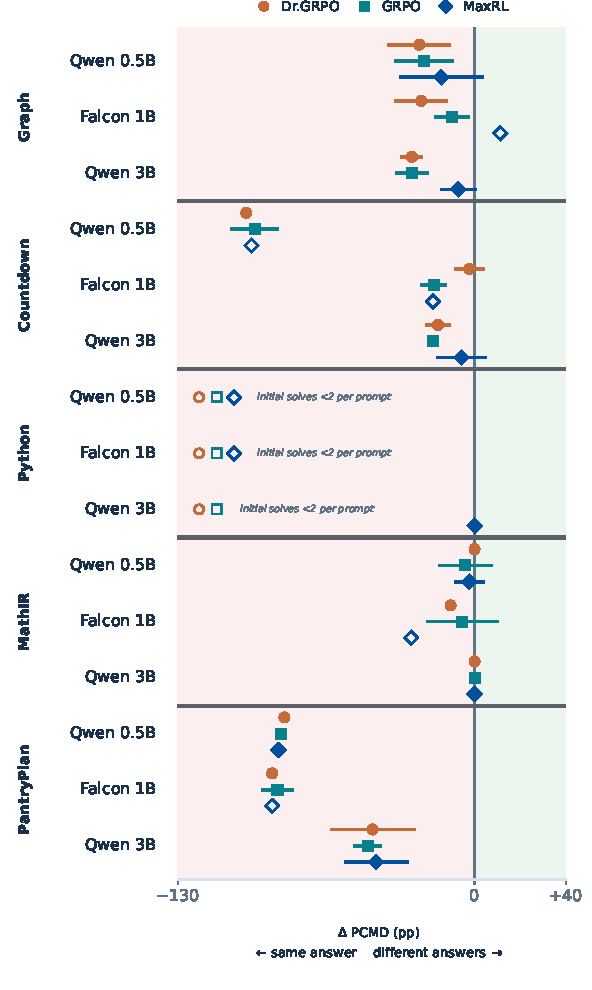
\includegraphics[width=\linewidth]{figures/concentration_story_all_scales.pdf}
  \end{minipage}\hfill
  \begin{minipage}[t]{.49\linewidth}
    \centering
    \textbf{(B)}\\[1pt]
    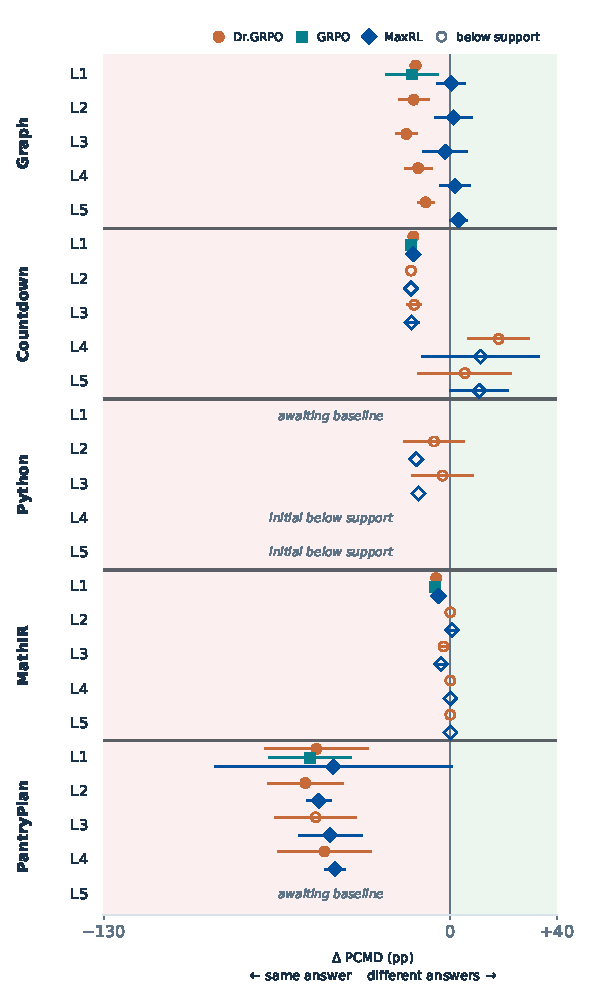
\includegraphics[width=\linewidth]{figures/concentration_levels.pdf}
  \end{minipage}
  \caption{\textbf{\texttt{Graph} and \texttt{PantryPlan} lose conditional solution diversity
  across scales and task levels.} Changes in \pmd{}, in percentage points.
  \textbf{(A)} Initial-to-final changes at Level~1 across three model scales
  and three objectives. Each seed averages over prompts with at least two
  correct responses at both checkpoints. Filled marks and bars show five-seed
  means and nominal paired 95\% Student-$t$ intervals. Open marks show
  means from fewer than five seeds, without intervals; annotated hollow
  symbols identify methods with no jointly eligible prompts. Dr.GRPO and GRPO reduce
  diversity in \texttt{Graph} and \texttt{PantryPlan} at every scale.
  \textbf{(B)} Level-1-trained policies evaluated on Levels~1--5, with
  Levels~2--5 measuring transfer. Available evaluations are averaged within
  each scale, then scales receive equal weight. Evaluations with different
  context limits contribute separately within a scale but do not constitute
  additional training seeds. Each scale uses one initial checkpoint evaluation.
  Bars appear only when one scale contributes and give nominal 95\%
  Student-$t$ intervals over its training seeds. Open marks indicate that at
  least one contributing scale has fewer than 30 eligible initial prompts or
  fewer than 30 eligible trained prompt observations in total. Missing initial
  references have fewer than two eligible prompts. GRPO appears only at
  Level~1. \texttt{Graph} and \texttt{PantryPlan} means decrease at every level; \texttt{Countdown}
  increases at Levels~4--5.}
  \label{fig:concentration-all-scales}
  \label{fig:concentration-levels}
\end{figure}


\subsection{Diversity before and after RLVR-only training}
\label{app:pre-rl-regression}

We evaluate Dr.GRPO and GRPO before training and after eight passes across
three models and five domains. The 150 runs each use four $K=8$ response
groups per checkpoint. Averaged equally across the five domains, extra
verified modes decrease by $98.2\%$--$99.4\%$ at Qwen2.5-0.5B and
$41.5\%$--$71.6\%$ at larger scales. The \texttt{pass@8} mean falls in
10 of the 30 domain--method--scale comparisons, while macro
\texttt{distinct@8} ends above its initial value at Qwen2.5-3B.
Fewer extra verified modes can therefore coexist with a greater probability
of sampling at least one correct response. Finite samples do not establish
that unobserved solution keys have zero probability.

\begin{samepage}
The domain average of \pmd{} includes only domains measurable at both endpoints: \texttt{Graph}, \texttt{MathIR}, and
\texttt{PantryPlan} at 0.5B; \texttt{Graph}, \texttt{Countdown}, and \texttt{PantryPlan} at 1B; and \texttt{Graph} and
\texttt{PantryPlan} at 3B. It declines by $98.5\%$ and $99.7\%$ at Qwen2.5-0.5B under
GRPO and Dr.GRPO, respectively, and by $50.8\%$--$65.1\%$ at the larger
scales. Terminal macro \pmd{} rounds to $.001$ for Dr.GRPO at Qwen2.5-0.5B.
The decline thus also appears in diversity conditional on success. Because
eligibility depends on the number of correct samples, these descriptive
averages do not hold the prompt population or correctness fixed.
App.~\ref{app:conditional-concentration} reports contrasts on jointly eligible
prompts. The decline is not universal: Falcon3-1B \texttt{Countdown} has
increasing \pmd{} under Dr.GRPO, from an initial value of $.033$.

\end{samepage}

Although the initial weights are shared, each method uses its own evaluation
samples. Differences between initial estimates therefore reflect sampling
variability.

\begin{figure}[t]
  \centering
  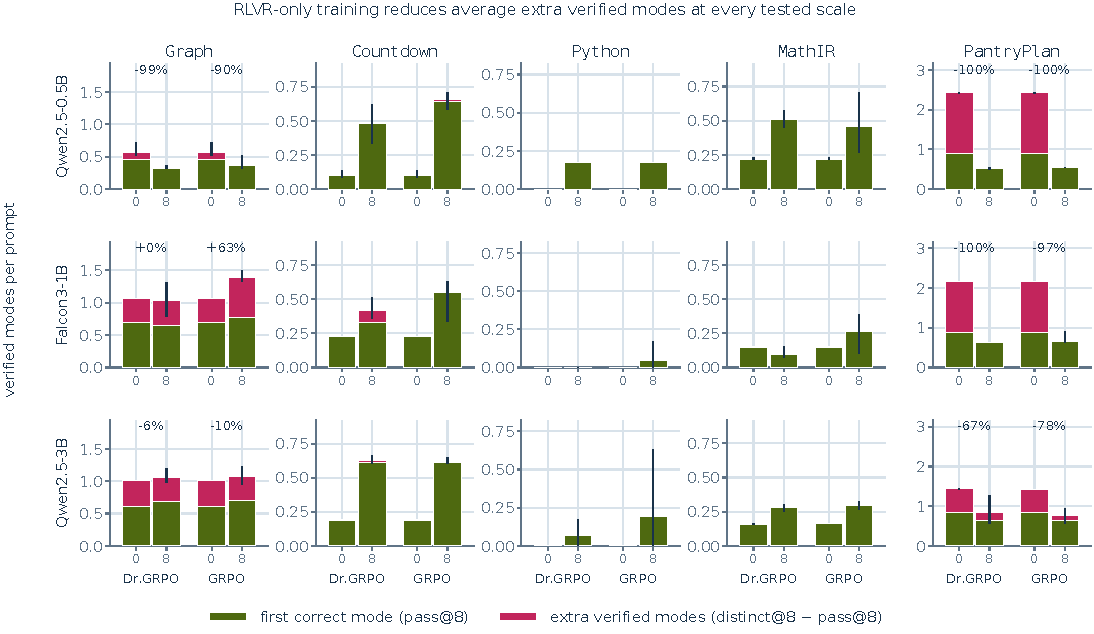
\includegraphics[width=\linewidth]{figures/baseline_collapse_precheck.pdf}
  \caption{\textbf{RLVR-only training reduces average extra verified modes
  at every tested scale.} Bars decompose \texttt{distinct@8} into
  \texttt{pass@8} and extra verified modes before training and after eight
  passes. Panels show Dr.GRPO and GRPO across three models and five domains:
  150 runs, with five seeds per model--domain--method combination and four
  eight-response groups per checkpoint. Whiskers show seed ranges; each
  method uses its own initial evaluation. Percentage changes in extra modes
  are shown for \texttt{Graph} and \texttt{PantryPlan}, whose initial means
  exceed $.05$. The other three domains start at $.011$ or less.}
  \label{fig:baseline-precheck}
\end{figure}




\texttt{Graph} and \texttt{PantryPlan} have substantial initial diversity at every
scale, whereas the other domains start with at most $.011$ extra modes per
prompt. To avoid unstable ratios near zero, retained-diversity percentages
are reported only when the initial extra-mode count exceeds $.05$.
The final $\texttt{distinct@8}$ is below its initial value in six of the
15 Dr.GRPO model--domain combinations. For Re:Dr, this occurs in two
available comparisons, both on \texttt{PantryPlan}; Falcon3-1B
\texttt{Countdown} uses four seeds. Conditional diversity comparisons
also depend on which prompts yield enough correct responses.
App.~\ref{app:conditional-concentration} reports paired contrasts on
jointly eligible prompts, including seed counts and uncertainty. These
held-out evaluations do not track individual modes stored during training.

Uniform sampling over the enumerable action representations gives a
diversity reference for \texttt{Graph} and \texttt{PantryPlan}
(App.~\ref{app:metric-sampling}). No corresponding reference is specified
for the other domains. On \texttt{PantryPlan}, uniform sampling of bit
masks yields higher expected \texttt{distinct@8} than the final sampled
value of every model under both Dr.GRPO and Re:Dr.

\begin{table}[t]
  \centering
  \caption{\textbf{Uniform actions and untrained checkpoints provide absolute diversity references.}
  \emph{Uniform} gives expected \distk{} under uniform sampling of the
  action representation: 27 color strings for \texttt{Graph} and 64 bit masks
  for \texttt{PantryPlan}. \emph{Initial} gives the Dr.GRPO pass-0 reference;
  the final two columns give sampled means after eight training passes.}
  \label{tab:absolute-support-references}
  \scriptsize
  \setlength{\tabcolsep}{4.2pt}
  \begin{tabular}{@{}llrrrr@{}}
    \toprule
    \textbf{Model} & \textbf{Domain} & \textbf{Uniform} & \textbf{Initial}
      & \textbf{Dr.GRPO} & \textbf{Re:Dr} \\
    \midrule
        \qwenmark{}2.5-0.5B & \texttt{Graph} & 1.633 & .561 & .325 & 2.438 \\
     & \texttt{PantryPlan} & 2.153 & 2.426 & .522 & 1.539 \\
    \addlinespace[2pt]
    Falcon3-1B & \texttt{Graph} & 1.633 & 1.070 & 1.034 & 1.717 \\
     & \texttt{PantryPlan} & 2.153 & 2.162 & .633 & 1.576 \\
    \addlinespace[2pt]
    \qwenmark{}2.5-3B & \texttt{Graph} & 1.633 & 1.012 & 1.060 & 1.637 \\
     & \texttt{PantryPlan} & 2.153 & 1.445 & .841 & 1.514 \\
    \bottomrule

  \end{tabular}
\end{table}


\subsection{Vanishing task gradients and repeated outputs}
\label{app:degenerate-groups}

A Dr.GRPO group with identical rewards has exactly zero fresh task gradient.
Only mixed groups, containing both correct and incorrect responses,
provide a nonzero task advantage. Optimizer momentum can still change the
policy when the current task gradient is zero. The table below reports
the fraction of mixed groups over 3,072 Qwen2.5-0.5B updates, averaged
across five seeds.

\begin{center}
\small
\begin{tabular}{@{}lrr@{}}
\toprule
\textbf{Domain} & \textbf{Dr.GRPO} & \textbf{Re:Dr} \\
\midrule
\texttt{Graph} & .144 & .954 \\
\texttt{Countdown} & .140 & .456 \\
\texttt{Python} & .015 & .185 \\
\texttt{MathIR} & .364 & .453 \\
\texttt{PantryPlan} & .123 & .789 \\
\bottomrule
\end{tabular}
\end{center}

Thus 98.5\% of \texttt{Python} control updates carry zero fresh task gradient.
Replay contributes a likelihood gradient from verified responses and can
also change the policy so that subsequent fresh groups contain both correct
and incorrect responses.

All five Qwen2.5-0.5B \texttt{Python} control seeds exhibit observed output collapse.
At pass 0, eight-response groups average 7.99 distinct completion strings
per prompt. By steps 288--480, all 32 temperature-1 responses for each
prompt are identical within each seed and match its greedy completion.
This holds on all 128 prompts and persists at every subsequent evaluation
through step 3,072. The 32 responses span four groups with overlapping sampling
streams (App.~\ref{app:conditional-concentration}); they are not 32 independent
draws. Within eight-response groups, the terminal mean is 1.00 distinct
completion per prompt for the control and 1.97 for replay. The repeated
completion can be incorrect. These finite observations do not rule out
low-probability alternatives.

This sparse binary-reward setting allows fresh task gradients to vanish.
Sampling strategies that favor mixed groups, larger groups, a reference-policy
KL penalty, token-entropy regularization, or broader decoding could change
this behavior. The present comparison does not isolate their effects.

\subsection{The controls learn at the fixed learning rates}
\label{app:control-learning-audit}

The controls use a constant learning rate of $2\times10^{-7}$ at
Qwen2.5-0.5B and Falcon3-1B and a peak rate of $10^{-7}$ with cosine decay
at Qwen2.5-3B (Table~\ref{tab:run-contract}). Learning rates are not swept.
Table~\ref{tab:control-learning-audit} reports changes in accuracy and the
frequency of informative response groups under these schedules. The
results characterize the tested settings without identifying an optimal
schedule for either method.

\begin{table}[t]
  \centering
  \caption{\textbf{Per-response accuracy increases in every control comparison,
  while \texttt{pass@8} can fall.} Accuracy compares initial and last
  available evaluations. Columns show unpaired five-run means for each
  model--domain combination. \texttt{mean@8} measures per-response
  correctness. Mixed gives the mean fraction of rollout groups
  containing both correct and incorrect responses. An unmixed group has
  zero fresh task advantage, although optimizer momentum can still change
  the policy. Training schedules match update counts and fresh-rollout
  budgets; total compute is discussed in App.~\ref{app:compute-accounting}.}
  \label{tab:control-learning-audit}
  \small
  \setlength{\tabcolsep}{5pt}
  \begin{tabular}{@{}llrrrrrrr@{}}
    \toprule
    & & \multicolumn{3}{c}{\textbf{control \texttt{pass@8}}}
      & \multicolumn{2}{c}{\textbf{control \texttt{mean@8}}}
      & \textbf{mixed} & \textbf{Re:Dr} \\
    \cmidrule(lr){3-5}\cmidrule(lr){6-7}
    \textbf{Model} & \textbf{Domain} & initial & terminal & $\Delta$
      & initial & terminal & groups & \texttt{pass@8} \\
    \midrule
    % Generated by ops/build_paper_control_learning_audit.py; do not hand edit.
    Qwen2.5-0.5B & \texttt{Graph} & .456 & .323 & $-$.132 & .178 & .323 & .144 & .969 \\
     & \texttt{Countdown} & .097 & .480 & $+$.383 & .014 & .465 & .140 & .672 \\
     & \texttt{Python} & .000 & .172 & $+$.172 & .000 & .172 & .015 & .528 \\
     & \texttt{MathIR} & .220 & .512 & $+$.292 & .037 & .464 & .364 & .796 \\
     & \texttt{PantryPlan} & .902 & .522 & $-$.380 & .344 & .522 & .123 & .729 \\
    \addlinespace[2pt]
    Falcon3-1B & \texttt{Graph} & .693 & .656 & $-$.037 & .178 & .300 & .777 & .809 \\
     & \texttt{Countdown} & .225 & .328 & $+$.103 & .037 & .268 & .400 & .636 \\
     & \texttt{Python} & .000 & .000 & $+$.000 & .000 & .000 & .009 & .979 \\
     & \texttt{MathIR} & .148 & .095 & $-$.053 & .023 & .068 & .158 & .736 \\
     & \texttt{PantryPlan} & .891 & .633 & $-$.258 & .318 & .633 & .523 & .751 \\
    \addlinespace[2pt]
    Qwen2.5-3B & \texttt{Graph} & .607 & .682 & $+$.075 & .215 & .360 & .706 & .836 \\
     & \texttt{Countdown} & .184 & .609 & $+$.426 & .049 & .569 & .281 & .746 \\
     & \texttt{Python} & .000 & .069 & $+$.069 & .000 & .069 & .011 & .659 \\
     & \texttt{MathIR} & .156 & .278 & $+$.122 & .061 & .168 & .152 & .686 \\
     & \texttt{PantryPlan} & .831 & .638 & $-$.193 & .267 & .558 & .482 & .744 \\
    \bottomrule

  \end{tabular}
\end{table}

\paragraph{Accuracy changes during training.}
Per-response correctness (\texttt{mean@8}) rises in all 15
control comparisons: every control learns under its schedule. What varies
is coverage. Using an absolute-change threshold of $.005$, 8 of the
15 comparisons improve in \texttt{pass@8} and
6 decline, so 7 controls gain per-response accuracy
without a \texttt{pass@8} increase above that threshold. The mean
\texttt{pass@8} change is +0.039; the largest increase is $+0.426$
(\texttt{Countdown} at Qwen2.5-3B) and the largest decrease is $-0.380$
(\texttt{PantryPlan} at Qwen2.5-0.5B). In \texttt{PantryPlan} at Falcon3-1B, per-response correctness rises from
0.318 to 0.633, while \texttt{pass@8}
falls from 0.891 to 0.633.
This combination is consistent with prior observations of increased
single-response accuracy alongside reduced sampling coverage
\citep{yue2025rlvrlimit}.

The gap between \texttt{pass@8} and \texttt{mean@8} is at least $.02$ in
12 initial model--domain comparisons and below $.02$ in
7 terminal comparisons. This gap reflects variation in
correctness within response groups; it does not identify repeated strings
or conditional diversity among correct solution keys. The completion-string
analysis in App.~\ref{app:degenerate-groups} directly measures repetition
for the Qwen2.5-0.5B \texttt{Python} controls.

\paragraph{Sparse fresh reward information.}
Initial \texttt{pass@8} is zero on \texttt{Python} at all three
scales. In \texttt{Python} at Falcon3-1B, only a fraction 0.009 of
updates contain mixed rewards, leaving zero fresh task advantage in
99.1\% of updates. A learning-rate change cannot make an
identically zero current task gradient nonzero, but it can change the effect
of informative updates, optimizer momentum, and subsequent sampling.
The Falcon3-1B \texttt{Python} control's terminal \texttt{pass@8} rounds to $.000$, while Re:Dr
ends at $.979$. This is an accuracy contrast in a sparse-success setting;
conditional mode diversity requires at least two correct responses per
prompt and is undefined when that sampling condition is unmet.

\paragraph{Scope of the comparison.}
Replay and control share the learning rate, schedule, initialization,
prompt stream, optimizer, update count, and fresh-rollout budget.
The comparison measures the effect of replay under these settings.
Per-response correctness increases in the controls, but the absence of a
learning-rate sweep limits conclusions about their optimal performance.
Other learning rates could change accuracy, diversity, and the relative
benefit of replay; the present results do not determine those changes.

The frequency of mixed groups helps characterize these comparisons.
When a control rarely produces mixed groups (App.~\ref{app:degenerate-groups}),
replay provides a likelihood gradient on updates with no fresh task advantage.
We therefore also summarize replay effects in subsets with increasing
control accuracy. Across all 15 model--domain combinations, the mean
Re:Dr minus Dr.GRPO effect is $+.352$ in \texttt{pass@8} and $+.189$
in \pmd{}. Among the 9 combinations with any positive initial-to-final
change in control \texttt{pass@8}, the effects are $+.379$ and $+.118$.
Among the 6 that also have nonzero initial \texttt{pass@8} and at least
10\% mixed rollout groups, they are $+.247$ and $+.136$. Every comparison
in these subsets has positive effects on both metrics; the smallest effects
in the six-comparison subset are $+.137$ in \texttt{pass@8} and $+.013$
in \pmd{}. Its mean diversity effect is about two thirds of the mean
across all comparisons. Table~\ref{tab:control-learning-audit} gives the
control measurements that define these subsets.

\subsection{Likelihood changes with a fixed replay buffer}
\label{app:fixed-bank-survival}

We examine the likelihoods of stored responses during Qwen2.5-0.5B Re:Dr
training on \texttt{Graph}, using five seeds. The buffer contents and counts
of fresh verified responses are held fixed from immediately before the
fresh rollout at step 384. Uniform replay continues through step 3,072
without adding modes. For each stored exemplar, identified by prompt and
canonical mode, we measure mean token log probability $s$ and sequence
log probability $\ell$ whenever it is replayed. Changes compare its first
and final replay visits after the buffer is fixed; these steps can differ
across exemplars.

The 3,406 exemplars span 1,575 seed--prompt pairs, with 8--9 replay visits
per exemplar.
The pooled median change is $+.038$ nat/token (95\% interval
$[+.025,+.048]$), while the 10th percentile is $-.256$ and $2.61\%$ of
exemplars lose more than $.5$ nat/token ($[1.54,3.77]\%$).
The largest observed intermediate decrease is $-1.328$ nat/token. Sequence log
probability has median change $+.154$ nat/sequence ($[+.104,+.198]$),
with $21.99\%$ of exemplars losing more than $.5$ nat/sequence.
Lengths range from 4 to 100 tokens, so the token and sequence thresholds
measure different changes.

\begin{figure}[!htbp]
  \centering
  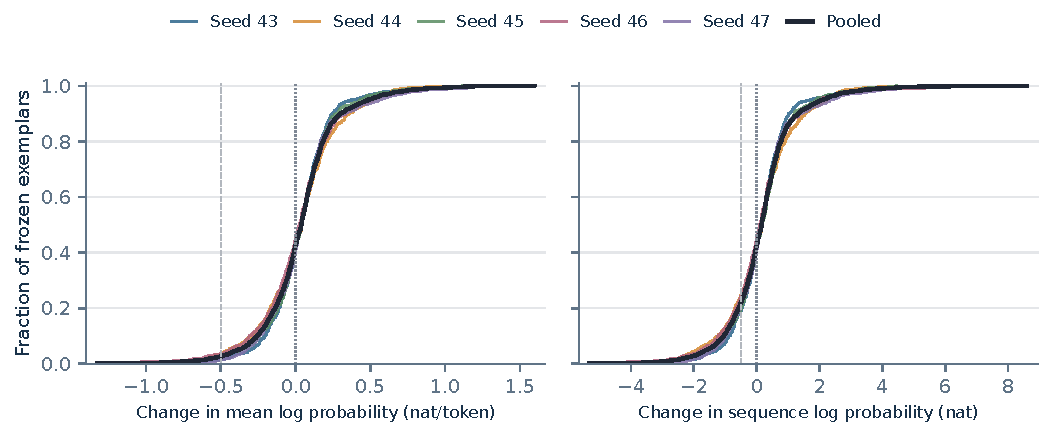
\includegraphics[width=.95\linewidth]{figures/e121_fixed_bank_survival.pdf}
  \caption{\textbf{Median exemplar scores rise, while some exemplars decline.}
  Empirical cumulative distributions of first-to-final score changes for
  3,406 fixed-buffer exemplars from five Qwen2.5-0.5B Re:Dr \texttt{Graph} seeds.
  Panels show mean token and sequence log probability. Colored curves
  represent individual seeds; the pooled curve weights exemplars equally.
  Dotted and dashed vertical lines mark zero and $-.5$, respectively.
  Positive changes indicate higher likelihood for the stored token sequence.
  Sequence likelihood does not measure the total probability of generating
  a canonical solution mode.}
  \label{fig:e121-fixed-bank-survival}
\end{figure}

Pooled summaries weight exemplars equally. Descriptive 95\% percentile
intervals use 10,000 hierarchical bootstrap replicates, resampling prompts
with replacement within each training seed and then resampling the five
seeds with replacement.

Scores are measured at replay visits, so changes between visits are
unobserved. Some stored exemplars lose likelihood despite continued replay.
A matched fixed-buffer control without replay would be needed to isolate
the effect of replay. These sequence-level observations also do not test
the mode-probability floor in Theorem~\ref{thm:replay-retention}.

\clearpage
\phantomsection
\begin{center}\large\textbf{Part IV. What diversity represents}\end{center}
\addcontentsline{toc}{part}{Part IV. What diversity represents}

\section{Matched Prompt-Hint Ablation}
\label{app:prompt-hint-ablation}

\subsection{Removing strategy hints from unchanged problems}

\label{sec:prompt-hint-ablation}

We compare original and neutral prompts on \texttt{Python}, \texttt{MathIR}, and \texttt{PantryPlan} at Levels 2 and 3. Each of the six domain--level combinations uses 32 problems selected independently of model outputs from the 128-problem evaluation split. We sample eight responses per problem under each wording. The original wording uses the standard prompt. The neutral wording removes the \texttt{Python} nested-conditional example and suggestions to test small divisors or dispatch on listed values, the \texttt{MathIR} ordered algebraic-isolation suggestion, and the \texttt{PantryPlan} preference for ingredients high in energy and protein but low in sodium such as seeds or oats. \texttt{MathIR} changes ``those operations'' to ``the operations'' to preserve the instruction to return a menu ID. The problem instance, answer specification, executable verifier, and remaining format requirements are unchanged.

The paired effects are neutral minus original on empirical $P_8=\texttt{pass@8}$ and $D_8=\texttt{distinct@8}$, with $B_8=D_8-P_8$ as extra verified modes per problem. Incorrect, empty, and truncated outputs remain in their eight-draw groups; only verifier-accepted outputs contribute a verified key. Results use strict verification. A sensitivity analysis with normalized formatting preserves every strict success and canonical key and applies the same rules to both arms.

Intervals use 20,000 whole-problem bootstrap resamples, paired across arms and stratified by domain and level. Domain--level combinations receive equal weight in aggregate estimates. The intervals are pointwise 95\% percentile intervals without multiplicity adjustment. With 32 problems per domain and level, an interval crossing zero does not establish equivalence. A zero-width interval reflects zero variation in the observed bootstrap resamples, including identical paired $P_8$ outcomes, and does not establish population equivalence. Correct-pair collision and its certified-support uniform reference use the same correct-pair weights. Eight draws per prompt do not identify total unseen support.



We evaluate the initial Qwen2.5-0.5B-Instruct checkpoint and Level-2-trained Dr.GRPO and Re:Dr checkpoints. \texttt{Python} and \texttt{MathIR} use five matched training seeds; \texttt{PantryPlan} uses two. Level 3 tests transfer from Level 2 training. All checkpoints evaluate the same selected problems under the benchmark syntax constraints and a 192-token generation budget. Five-seed intervals resample whole training seeds and paired problems; \texttt{PantryPlan} intervals condition on its two checkpoints, and initial-model intervals condition on one instruction-tuned checkpoint. These effects concern the specified models, problems, and interface.


\begin{table}[t]
\centering
\scriptsize
\setlength{\tabcolsep}{2.2pt}
\caption{\textbf{Removing \texttt{Python} guidance reduces correctness and observed breadth.} Qwen2.5-0.5B checkpoints under strict verification, with original $\to$ neutral wording. $P_8=\texttt{pass@8}$, $D_8=\texttt{distinct@8}$, and $B_8=D_8-P_8$ use eight draws on each of 32 problems per domain and level. Effects are neutral minus original. $P_8$, $D_8$, and $B_8$ average the displayed number $s$ of checkpoints. Brackets are pointwise 95\% bootstrap intervals: paired problems and training seeds are resampled for five-seed groups; \texttt{PantryPlan} intervals condition on its two checkpoints, and initial-model intervals on one checkpoint. \pmd{} estimates the probability that two correct responses have different canonical keys, averaging checkpoint--problem groups with at least two verified draws in each arm. Its paired population depends on correctness, and repeated problems at different checkpoints count separately. Only 5 of 18 comparisons meet the minimum of 30 such groups; dashes denote the others. These \pmd{} point estimates have no reported uncertainty intervals.}
\label{tab:prompt-hints-local-strict}
\resizebox{\linewidth}{!}{%
\begin{tabular}{llrrrrrrr}
\toprule
Model & Domain/level & $P_8$: O$\to$N & $D_8$: O$\to$N & $\Delta P_8$ [95\%] & $\Delta D_8$ [95\%] & $\Delta B_8$ & \pmd{}: O$\to$N & $\Delta$ \pmd{} \\
\midrule
Initial ($s=1$) & \texttt{Python} L2 & $0.656\to0.125$ & $0.69\to0.12$ & $-0.531\;[-0.719,-0.344]$ & $-0.56\;[-0.75,-0.38]$ & $-0.03$ & -- & -- \\
Initial ($s=1$) & \texttt{MathIR} L2 & $0.250\to0.281$ & $0.25\to0.28$ & $+0.031\;[+0.000,+0.094]$ & $+0.03\;[+0.00,+0.09]$ & $+0.00$ & -- & -- \\
Initial ($s=1$) & \texttt{PantryPlan} L2 & $0.156\to0.188$ & $0.19\to0.22$ & $+0.031\;[+0.000,+0.094]$ & $+0.03\;[+0.00,+0.09]$ & $+0.00$ & -- & -- \\
Initial ($s=1$) & \texttt{Python} L3 & $0.719\to0.031$ & $0.81\to0.03$ & $-0.688\;[-0.844,-0.531]$ & $-0.78\;[-0.97,-0.59]$ & $-0.09$ & -- & -- \\
Initial ($s=1$) & \texttt{MathIR} L3 & $0.219\to0.219$ & $0.22\to0.22$ & $+0.000\;[-0.125,+0.125]$ & $+0.00\;[-0.12,+0.12]$ & $+0.00$ & -- & -- \\
Initial ($s=1$) & \texttt{PantryPlan} L3 & $0.281\to0.312$ & $0.66\to0.69$ & $+0.031\;[+0.000,+0.094]$ & $+0.03\;[-0.06,+0.12]$ & $+0.00$ & -- & -- \\
Dr.GRPO ($s=5$) & \texttt{MathIR} L2 & $0.531\to0.506$ & $0.53\to0.51$ & $-0.025\;[-0.100,+0.031]$ & $-0.03\;[-0.10,+0.03]$ & $+0.00$ & $.000\to.000$ & $+.000$ \\
Dr.GRPO ($s=5$) & \texttt{MathIR} L3 & $0.194\to0.156$ & $0.19\to0.16$ & $-0.037\;[-0.113,+0.019]$ & $-0.04\;[-0.11,+0.02]$ & $+0.00$ & -- & -- \\
Dr.GRPO ($s=2$) & \texttt{PantryPlan} L2 & $0.219\to0.203$ & $0.28\to0.25$ & $-0.016\;[-0.156,+0.125]$ & $-0.03\;[-0.19,+0.12]$ & $-0.02$ & -- & -- \\
Dr.GRPO ($s=2$) & \texttt{PantryPlan} L3 & $0.172\to0.172$ & $0.27\to0.25$ & $+0.000\;[-0.078,+0.078]$ & $-0.02\;[-0.16,+0.11]$ & $-0.02$ & -- & -- \\
Dr.GRPO ($s=5$) & \texttt{Python} L2 & $0.812\to0.000$ & $0.81\to0.00$ & $-0.812\;[-0.938,-0.656]$ & $-0.81\;[-0.94,-0.66]$ & $+0.00$ & -- & -- \\
Dr.GRPO ($s=5$) & \texttt{Python} L3 & $1.000\to0.000$ & $1.00\to0.00$ & $-1.000\;[-1.000,-1.000]$ & $-1.00\;[-1.00,-1.00]$ & $+0.00$ & -- & -- \\
Re:Dr ($s=5$) & \texttt{MathIR} L2 & $0.994\to0.975$ & $0.99\to0.97$ & $-0.019\;[-0.075,+0.000]$ & $-0.02\;[-0.07,+0.00]$ & $+0.00$ & $.000\to.000$ & $+.000$ \\
Re:Dr ($s=5$) & \texttt{MathIR} L3 & $0.312\to0.275$ & $0.31\to0.28$ & $-0.037\;[-0.138,+0.044]$ & $-0.04\;[-0.14,+0.04]$ & $+0.00$ & $.000\to.000$ & $+.000$ \\
Re:Dr ($s=2$) & \texttt{PantryPlan} L2 & $0.516\to0.500$ & $0.75\to0.73$ & $-0.016\;[-0.109,+0.078]$ & $-0.02\;[-0.20,+0.17]$ & $+0.00$ & -- & -- \\
Re:Dr ($s=2$) & \texttt{PantryPlan} L3 & $0.234\to0.281$ & $0.39\to0.50$ & $+0.047\;[+0.000,+0.109]$ & $+0.11\;[+0.05,+0.19]$ & $+0.06$ & -- & -- \\
Re:Dr ($s=5$) & \texttt{Python} L2 & $0.887\to0.556$ & $1.24\to0.68$ & $-0.331\;[-0.525,-0.150]$ & $-0.57\;[-0.85,-0.32]$ & $-0.24$ & $.231\to.173$ & $-.058$ \\
Re:Dr ($s=5$) & \texttt{Python} L3 & $1.000\to0.494$ & $1.42\to0.66$ & $-0.506\;[-0.825,-0.194]$ & $-0.76\;[-1.07,-0.38]$ & $-0.26$ & $.256\to.323$ & $+.067$ \\
\bottomrule
\end{tabular}}
\end{table}


\pmd{} is reported for five of the 18 comparisons in Table~\ref{tab:prompt-hints-local-strict}. Each requires at least thirty checkpoint--problem groups with at least two verified draws under each wording. The same 32 problems are evaluated at each checkpoint, so these group counts include repeated problems across training seeds. Within a comparison, \pmd{} weights eligible groups equally; checkpoints with more eligible problems therefore receive more weight. The population depends on success under both wordings and need not represent all evaluated problems. Three eligible comparisons are \texttt{MathIR}: all observed verified pairs within each eligible group share a canonical key, giving \pmd{} $=.000$ under both wordings. This observation does not limit the number of valid keys. In the two Re:Dr comparisons on \texttt{Python}, hint removal changes \pmd{} from $.231$ to $.173$ at Level 2 and from $.256$ to $.323$ at Level 3, on 66 and 57 eligible checkpoint--problem groups, respectively. The two point estimates have opposite signs; without intervals, they do not establish a shared direction or the reliability of either concentration effect. At Level 3, conditional diversity uses four training seeds, while $P_8$ and $D_8$ use all five; the fifth seed has too few jointly verified responses. A dash denotes an unavailable conditional estimate, not a zero effect.


Formatting normalization adds no verified responses for any Qwen2.5-0.5B checkpoint in this panel; all tabulated estimates and intervals therefore agree under the two grading rules.


\begin{figure}[t]

\centering

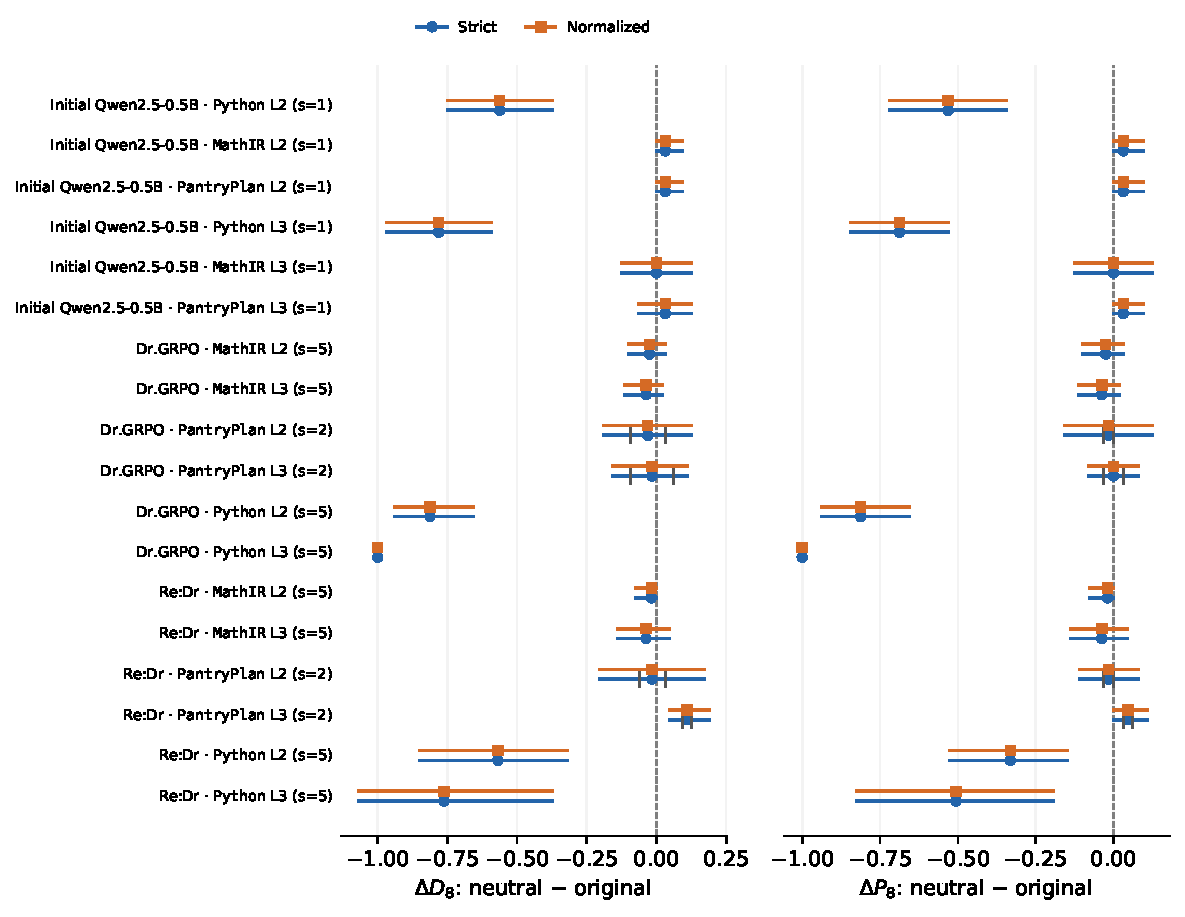
\includegraphics[width=\linewidth]{figures/modebench_prompt_ablation_local.pdf}

\caption{\textbf{\texttt{Python} guidance removal produces the largest wording effects in this panel.} Neutral-minus-original $D_8$ (left) and $P_8$ (right) for the initial Qwen2.5-0.5B checkpoint and Level-2-trained Dr.GRPO and Re:Dr on \texttt{Python}, \texttt{MathIR}, and \texttt{PantryPlan} at Levels 2 and 3, with 32 paired problems and eight draws per arm. Blue circles use strict verification; orange squares use formatting normalization. Horizontal bars are pointwise 95\% bootstrap intervals; the vertical dashed line marks zero. Five-seed groups resample training seeds and paired problems; \texttt{PantryPlan} and initial-model intervals condition on two checkpoints and one checkpoint, respectively. Gray marks show the individual effects for the two \texttt{PantryPlan} training seeds. }

\label{fig:prompt-hints-local}

\end{figure}



\begin{samepage}
\paragraph{Two-seed \texttt{PantryPlan} effects.} Intervals condition on the two checkpoints and do not quantify training-seed variability. The effects for each seed are shown below; each pair gives $(\Delta P_8,\Delta D_8)$.
\begin{center}\small
\begin{tabular}{llcc}
\toprule
Method & Level & First seed & Second seed \\
\midrule
Dr.GRPO & 2 & $(+0.000, +0.03)$ & $(-0.031, -0.09)$ \\
Dr.GRPO & 3 & $(+0.031, +0.06)$ & $(-0.031, -0.09)$ \\
Re:Dr & 2 & $(-0.031, -0.06)$ & $(+0.000, +0.03)$ \\
Re:Dr & 3 & $(+0.031, +0.12)$ & $(+0.062, +0.09)$ \\
\bottomrule
\end{tabular}
\end{center}
\end{samepage}

\paragraph{Scope of the wording intervention.}
The \texttt{Python} intervention removes an executable nested-conditional example
along with divisor-testing and dispatch guidance, and it shortens the prompt.
Its effect concerns this combined change; it does not isolate a preference
cue from example or length effects. Lower \texttt{distinct@8} together with
lower \texttt{pass@8} can reflect reduced correctness rather than increased
concentration among correct outputs. The \pmd{} columns in
Table~\ref{tab:prompt-hints-local-strict} measure conditional diversity on
jointly eligible checkpoint--problem groups. Eligibility itself depends on
correctness, so these comparisons do not hold the full evaluation population
or its accuracy fixed.

\paragraph{Observed prompt dependence.}
\texttt{Python} shows a large loss of correctness after guidance removal. Across the
five Dr.GRPO seeds, mean $P_8$ falls from $.8125$ to zero at Level~2 and from
$1.0$ to zero at Level~3; $D_8$ falls identically and $B_8=0$ in both arms.
With no correct neutral Dr.GRPO outputs, its concentration among correct outputs
is undefined. Re:Dr retains neutral $P_8=.55625$ and $.49375$ and
$D_8=.675$ and $.65625$ at Levels~2 and~3, respectively, while losing
extra verified modes: $\Delta B_8=-.2375$ and $-.25625$. The initial checkpoint
also loses \texttt{Python} correctness (Table~\ref{tab:prompt-hints-local-strict}).
These observations identify substantial dependence on the combined \texttt{Python}
wording intervention; a raw mode-count decline cannot be interpreted solely
as a redistribution among correct answers.


\paragraph{\texttt{Python} responses after hint removal.}
Across 5,120 Dr.GRPO \texttt{Python} responses from five seeds, two levels, and both
wordings, all 2,560 outputs generated with the original wording yield the
same extracted lambda expression, whose body matches the conditional
example in the prompt; 2,320 of these
responses pass verification:
\begin{quote}\footnotesize\ttfamily
lambda n: 2 if n \% 2 == 0 else 3 if n \% 3 == 0 else 5
\end{quote}
\begin{samepage}
Of the 2,560 neutral-wording responses, 1,816 (70.94\%) are invalid Python
expressions, 59 violate other restricted-language rules, 376 return
non-integers, 276 fail the proper-divisor condition, and 33 (1.29\%) have
no extracted candidate after reaching the token limit. Syntax errors are
the largest failure category. The categories follow the first rejection
during extraction, parsing, and execution. They describe output failures
without identifying the training mechanism responsible.

\end{samepage}

\paragraph{Concentration after hint removal.}
Every trained \texttt{MathIR} checkpoint has $B_8=0$ under both wordings at both levels.
Within each problem's eight-draw group, every observed pair of correct
outputs shares a canonical key at every trained checkpoint and level:
correct-pair collision is $1.0$, versus the
uniform reference of $.2$ over five certified modes.
Table~\ref{tab:prompt-hints-local-strict} reports \pmd{} $.000$ under both
wordings in every eligible \texttt{MathIR} comparison. Removing this hint therefore leaves
observed correct outputs concentrated. At Level~2, Re:Dr retains mean $P_8=.975$ without the order hint, compared with $.99375$
with it. Across its five checkpoints, the neutral arm has 4,179 colliding
pairs out of 4,179 correct pairs, from 154 eligible checkpoint--problem
groups; the original arm has 4,382 out of 4,382 pairs from 157 such groups.
Both arms evaluate the same 32 problems at each checkpoint. Thus observed concentration persists after removing the order hint.
The comparison does not measure unseen modes, and the remaining interface
constraints still apply.
\texttt{PantryPlan} effects are mixed. Re:Dr at Level~3 gains $.109375$ in $D_8$,
comprising $.046875$ in $P_8$ and $.0625$ in $B_8$, but this comparison has only
two training seeds. App.~\ref{app:sampling-budget-ablation} evaluates
hosted models under both wordings with 64 draws on sixteen problems per
domain--level combination. Its problem population and sampling budget
differ from the eight-draw evaluation here.


\section{Decoding Temperature, Nucleus, and Budget}
\label{app:decoding-objection}

\paragraph{Temperature at fixed checkpoints.}
Qwen2.5-0.5B Dr.GRPO and Re:Dr checkpoints after eight training passes are
evaluated at $T\in\{.5,.7,1.0,1.3,1.6,2.0\}$, with top-$p=1$ and four
eight-response groups per prompt. Five domains, two methods, and five seeds
give 300 checkpoint--setting evaluations (Fig.~\ref{fig:decoding-objection}A).
The prompt template, evaluation split, response limit, and sampling seeds
are fixed across temperatures. Correct keys are pooled across response
groups for each prompt; the groups have overlapping sampling streams
(App.~\ref{app:conditional-concentration}). Estimates therefore describe
these sampled pools. A seed contributes to the \pmd{} mean when at least
30 prompts yield at least two correct responses. Eligible prompts and seeds
can differ across temperatures and methods.

Across the six temperatures, the largest control \pmd{} is $.021$ in
\texttt{Graph}, $.016$ in \texttt{Countdown}, $.002$ in \texttt{MathIR}, and $.004$ in \texttt{PantryPlan}.
Re:Dr at $T=1$ has corresponding means $.562$, $.485$, $.020$, and $.330$.
These four domains retain five eligible control seeds at every temperature.
\texttt{Python} controls have no seed reaching the 30-prompt threshold, so their
conditional diversity is unidentified under this reporting rule.
The sweep therefore shows low measured control diversity in the four
eligible domains, without establishing that unobserved modes have zero
probability or that every decoding choice would behave the same way.

\paragraph{Hardware sensitivity.}
All evaluations in the temperature sweep use NVIDIA RTX A5000 GPUs.
A paired comparison of A100 and A5000 evaluations at $T=1$ gives mean
absolute \pmd{} difference $.0032$ across twelve comparisons, with maximum
$.0131$. These differences describe the tested hardware comparisons;
they do not bound hardware sensitivity at other checkpoints or settings.

\paragraph{Larger groups and nucleus truncation.}
A separate set of Qwen2.5-0.5B checkpoints trained for twelve passes is evaluated at
eleven settings (Fig.~\ref{fig:decoding-objection}B): the six temperatures
above; two groups of $K=32$ at $T\in\{1.0,1.3,1.6\}$; and four groups
of $K=8$ with top-$p=.95$ at $T\in\{1.0,1.6\}$. The $K=32$ settings
quadruple the group size and double total responses per prompt from 32 to
64. Five domains, two methods, and five seeds give 550 checkpoint--setting
evaluations. The replay variant combines separate mass and within-buffer
balancing terms with novelty and semantic-entropy shaping. Its objective
and training duration therefore differ from the eight-pass Re:Dr comparison.

Control \pmd{} is zero throughout the grid in \texttt{Graph}. Its range is $.006$
to $.031$ in \texttt{Countdown}, $.000$ to $.003$ in \texttt{MathIR}, and $.037$ to $.069$
in \texttt{PantryPlan}.
All eleven settings retain five eligible control seeds in these domains;
\texttt{Python} controls remain below the reporting threshold. The replay markers
provide a descriptive reference for this separate variant, without
identifying the effect of the Re:Dr objective.

Three comparisons hold temperature and nucleus sampling fixed while
increasing both group size and total response budget: $K=8$ and $K=32$ at
$T\in\{1.0,1.3,1.6\}$, top-$p=1$. Across these matched settings, control
\pmd{} changes by at most $.010$ in absolute value, and no
$K=32$ control mean exceeds $.054$. \texttt{Graph} stays at $.000$;
\texttt{Countdown} moves from $.014$--$.027$ to $.013$--$.023$;
\texttt{MathIR} from $.000$--$.001$ to $.001$--$.003$; and \texttt{PantryPlan}
from $.050$--$.063$ to $.045$--$.053$. Each mean uses five eligible seeds.
The larger budget therefore does not move these controls out of their
low-\pmd{} range. This compares sampled pools at fixed checkpoints; it does
not establish that unobserved modes carry zero probability.

\begin{figure}[t]
  \centering
  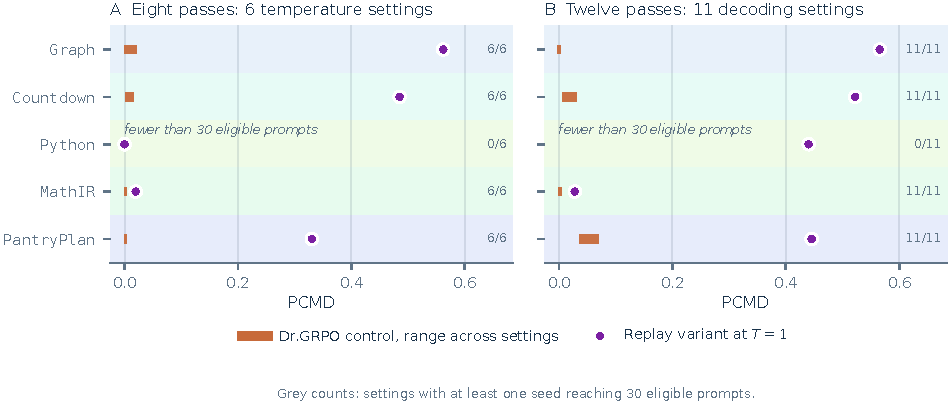
\includegraphics[width=\linewidth]{figures/decoding_objection.pdf}
  \caption{\textbf{Control diversity remains low across the tested decoding
  settings.} Qwen2.5-0.5B terminal \pmd{} across five domains.
  \textbf{(A)} Eight-pass Dr.GRPO/Re:Dr checkpoints at six temperatures
  ($T=.5$--$2.0$): 300 checkpoint--setting evaluations.
  \textbf{(B)} Separate twelve-pass checkpoints at eleven temperature, group-size,
  and nucleus settings: 550 evaluations, using a different replay objective.
  Bars span control means across settings; they are not confidence intervals.
  Markers show the corresponding replay variant at $T=1$, top-$p=1$,
  and $K=8$. Means use seeds with at least 30 prompts having at least two correct
  responses, so control and replay populations need not match. Control bars
  use five seeds outside \texttt{Python}; \texttt{Python} controls have none, while its replay
  markers use two seeds in A and three in B. Counts give eligible settings.
  Ranges narrower than $.004$ are displayed at width $.004$ for visibility.}
  \label{fig:decoding-objection}
\end{figure}

\paragraph{Scope of the decoding comparison.}
Both grids evaluate fixed terminal policies at one model scale. They do not
measure the effects of changing rollout temperature, optimizer settings, or
training duration. Correctness and conditional eligibility can change with
decoding settings; a missing \pmd{} estimate indicates insufficient eligible
prompts, rather than disappearance of all correct solution modes.

\section{Sampling-Budget Ablation}
\label{app:sampling-budget-ablation}

\subsection{Sampling design and estimands}
\label{sec:discovery-curves}
Large-budget \texttt{pass@k} evaluation can reveal differences hidden at smaller budgets \citep{yue2025rlvrlimit}. We evaluate sixteen problems from each of \texttt{Python}, \texttt{MathIR}, and \texttt{PantryPlan} at Levels~2 and~3.

Problems are selected independently of model outputs from the prompt-hint ablation population. Each has original and neutral wordings, with 64 responses per wording from each checkpoint or deployment. Eight-draw estimates use subsets of these same response pools. The initial Qwen2.5-0.5B-Instruct checkpoint has no training-seed replication. Dr.GRPO and Re:Dr use five matched seeds in \texttt{Python} and \texttt{MathIR} and two in \texttt{PantryPlan}. These checkpoints are trained at Level~2, so Level~3 measures transfer.

For a 64-draw pool, let $c$ be the number of correct outputs and $n_j$ the count of verified canonical key $j$. At $k\in\{1,2,4,8,16,32,64\}$, we average over all size-$k$ subsets without replacement:
\[
 P_k=1-\frac{\binom{64-c}{k}}{\binom{64}{k}},\qquad
 D_k=\sum_j\left[1-\frac{\binom{64-n_j}{k}}{\binom{64}{k}}\right],\qquad B_k=D_k-P_k.
\]
Here $P_k$ is the probability of at least one correct response, $D_k$ is the expected number of distinct verified modes, and $B_k$ is the expected number of modes beyond the first success. Infeasible numerator combinations are zero. Incorrect, empty, refused, and truncated responses remain in the pool; only verifier-accepted responses contribute keys. The curve points are correlated because they share a response pool and describe finite-sample discovery. The gains $G_P=P_{64}-P_8$, $G_D=D_{64}-D_8$, and $G_B=B_{64}-B_8$ distinguish improvements in first-success probability from the discovery of additional modes; they do not estimate complete unseen support.

We report strict-verifier results and a formatting-normalization sensitivity analysis that preserves every strict success and canonical key. Intervals use 20,000 whole-problem bootstrap replicates, paired across wordings and stratified by domain and level. Five-seed intervals also resample matched training seeds with shared problem indices; \texttt{PantryPlan} intervals condition on its two checkpoints. Each domain--level comparison contains sixteen problems, and intervals are unadjusted for multiple comparisons. Zero-width intervals indicate no observed resampled variation and do not establish equivalence.

For breadth at a fixed number of correct draws, we average over subsets of $m$ correct responses:
\[
 R_m=\sum_j\left[1-\frac{\binom{c-n_j}{m}}{\binom{c}{m}}\right].
\]
Paired comparisons require $c\ge m$ under both wordings. They therefore condition on observed success, without equating accuracy or estimating diversity for excluded problems.

Eligibility varies with $m$, method, and grading. Trained-checkpoint means weight seeds equally and are undefined if any seed lacks eligible prompts. Conditional intervals retain only bootstrap replicates in which the corresponding mean is defined.

The 64-draw summaries use two prompt weightings. Pooled collision $C$ divides the total number of equal-key correct pairs by the total number of correct pairs within each checkpoint or deployment; a prompt therefore receives weight proportional to $\binom{c}{2}$. Promptwise \pmd{} averages $1-\sum_j\binom{n_j}{2}/\binom{c}{2}$ equally over prompts with $c\ge2$. Each wording's absolute estimate uses its own eligible prompts, whereas the neutral-minus-original contrast $\Delta\pmd$ uses only jointly eligible prompts. Trained-checkpoint estimates then receive equal weight across seeds.

Support references use certified lower bounds $L\le M$: two valid modes in \texttt{Python}, five in \texttt{MathIR}, and the problem-specific certificate count in \texttt{PantryPlan}. Thus $1/L$ is an upper reference for collision under a uniform distribution over full support, and $L[1-(1-1/L)^m]$ is a lower reference for uniform expected breadth. These references describe uniform sampling; they do not bound model breadth, and observed distinct counts may exceed $L$.

In the tables, O/N denotes original/neutral wording, and $\Delta G_D$ is the neutral-minus-original discovery gain. $U$ denotes the uniform reference under the corresponding weighting. $E_O/E_N$ count separately eligible checkpoint--problem pairs with $c\ge2$; $Q_O/Q_N$ count correct response pairs. The counts sum across checkpoints, whereas the estimates weight checkpoints equally. Separate eligibility counts do not give the size of the jointly eligible population used for a contrast.


\begin{table}[!htbp]
\centering\scriptsize
\setlength{\tabcolsep}{3pt}
\caption{\textbf{Discovery gains from eight to 64 draws.} Strict verification; O/N denotes original/neutral wording. Each row reports sixteen problems for one deployment, domain, and level. Intervals resample paired problems, with no replication across model training seeds.}
\label{tab:discovery-gains-frontier-strict}
\resizebox{\linewidth}{!}{%
\begin{tabular}{llrrrr}
\toprule
Model & Domain/level & $G_P$: O/N & $G_D$: O/N & $G_B$: O/N & $\Delta G_D$ [95\%] \\
\midrule
GPT-5.4 & \texttt{Python} L2 & $0.014/0.000$ & $2.017/3.051$ & $2.003/3.051$ & $+1.033\;[-0.044,+2.371]$ \\
GPT-5.6 Sol & \texttt{Python} L2 & $0.000/0.405$ & $0.000/0.866$ & $0.000/0.462$ & $+0.866\;[+0.545,+1.231]$ \\
Grok 4.3 & \texttt{Python} L2 & $0.000/0.000$ & $0.667/1.013$ & $0.667/1.013$ & $+0.346\;[-0.583,+1.128]$ \\
GPT-5.4 & \texttt{Python} L3 & $0.025/0.000$ & $2.100/2.340$ & $2.076/2.340$ & $+0.240\;[-0.379,+0.930]$ \\
GPT-5.6 Sol & \texttt{Python} L3 & $0.000/0.586$ & $0.000/0.759$ & $0.000/0.174$ & $+0.759\;[+0.581,+0.952]$ \\
Grok 4.3 & \texttt{Python} L3 & $0.000/0.000$ & $0.424/1.576$ & $0.424/1.576$ & $+1.152\;[+0.640,+1.689]$ \\
GPT-5.4 & \texttt{MathIR} L2 & $0.043/0.042$ & $0.043/0.909$ & $0.000/0.868$ & $+0.867\;[+0.587,+1.111]$ \\
GPT-5.6 Sol & \texttt{MathIR} L2 & $0.027/0.004$ & $0.027/0.686$ & $0.000/0.682$ & $+0.659\;[+0.416,+0.888]$ \\
Grok 4.3 & \texttt{MathIR} L2 & $0.000/0.001$ & $0.223/0.322$ & $0.223/0.321$ & $+0.099\;[-0.226,+0.438]$ \\
GPT-5.4 & \texttt{MathIR} L3 & $0.000/0.000$ & $0.055/0.663$ & $0.055/0.663$ & $+0.609\;[+0.342,+0.888]$ \\
GPT-5.6 Sol & \texttt{MathIR} L3 & $0.000/0.000$ & $0.000/0.515$ & $0.000/0.515$ & $+0.515\;[+0.318,+0.714]$ \\
Grok 4.3 & \texttt{MathIR} L3 & $0.000/0.000$ & $0.167/0.805$ & $0.167/0.805$ & $+0.638\;[+0.348,+0.935]$ \\
GPT-5.4 & \texttt{PantryPlan} L2 & $0.001/0.015$ & $1.158/2.583$ & $1.156/2.568$ & $+1.426\;[+0.423,+2.641]$ \\
GPT-5.6 Sol & \texttt{PantryPlan} L2 & $0.086/0.101$ & $0.917/1.789$ & $0.831/1.688$ & $+0.872\;[+0.245,+1.575]$ \\
Grok 4.3 & \texttt{PantryPlan} L2 & $0.000/0.000$ & $1.022/3.377$ & $1.022/3.377$ & $+2.354\;[+1.592,+3.123]$ \\
GPT-5.4 & \texttt{PantryPlan} L3 & $0.000/0.002$ & $1.666/3.219$ & $1.666/3.218$ & $+1.553\;[+0.776,+2.367]$ \\
GPT-5.6 Sol & \texttt{PantryPlan} L3 & $0.032/0.129$ & $1.625/1.842$ & $1.592/1.713$ & $+0.217\;[-0.489,+0.921]$ \\
Grok 4.3 & \texttt{PantryPlan} L3 & $0.000/0.000$ & $1.810/4.466$ & $1.810/4.466$ & $+2.656\;[+1.698,+3.640]$ \\
\bottomrule
\end{tabular}}
\end{table}

\begin{table}[!htbp]
\centering\scriptsize
\setlength{\tabcolsep}{3pt}
\caption{\textbf{Discovery gains from eight to 64 draws.} Formatting normalization; O/N denotes original/neutral wording. Each row reports sixteen problems for one deployment, domain, and level. Intervals resample paired problems, with no replication across model training seeds.}
\label{tab:discovery-gains-frontier-normalized-secondary}
\resizebox{\linewidth}{!}{%
\begin{tabular}{llrrrr}
\toprule
Model & Domain/level & $G_P$: O/N & $G_D$: O/N & $G_B$: O/N & $\Delta G_D$ [95\%] \\
\midrule
GPT-5.4 & \texttt{Python} L2 & $0.000/0.000$ & $2.156/3.216$ & $2.156/3.216$ & $+1.060\;[-0.071,+2.386]$ \\
GPT-5.6 Sol & \texttt{Python} L2 & $0.008/0.010$ & $0.113/0.794$ & $0.105/0.784$ & $+0.681\;[+0.351,+1.066]$ \\
Grok 4.3 & \texttt{Python} L2 & $0.000/0.000$ & $0.667/1.013$ & $0.667/1.013$ & $+0.346\;[-0.583,+1.128]$ \\
GPT-5.4 & \texttt{Python} L3 & $0.000/0.000$ & $2.431/2.604$ & $2.431/2.604$ & $+0.173\;[-0.657,+1.075]$ \\
GPT-5.6 Sol & \texttt{Python} L3 & $0.011/0.007$ & $0.120/0.490$ & $0.109/0.483$ & $+0.370\;[+0.112,+0.674]$ \\
Grok 4.3 & \texttt{Python} L3 & $0.000/0.000$ & $0.424/1.576$ & $0.424/1.576$ & $+1.152\;[+0.640,+1.689]$ \\
GPT-5.4 & \texttt{MathIR} L2 & $0.043/0.042$ & $0.043/0.909$ & $0.000/0.868$ & $+0.867\;[+0.587,+1.111]$ \\
GPT-5.6 Sol & \texttt{MathIR} L2 & $0.027/0.004$ & $0.027/0.686$ & $0.000/0.682$ & $+0.659\;[+0.416,+0.888]$ \\
Grok 4.3 & \texttt{MathIR} L2 & $0.000/0.001$ & $0.223/0.322$ & $0.223/0.321$ & $+0.099\;[-0.226,+0.438]$ \\
GPT-5.4 & \texttt{MathIR} L3 & $0.000/0.000$ & $0.055/0.663$ & $0.055/0.663$ & $+0.609\;[+0.342,+0.888]$ \\
GPT-5.6 Sol & \texttt{MathIR} L3 & $0.000/0.000$ & $0.000/0.515$ & $0.000/0.515$ & $+0.515\;[+0.318,+0.714]$ \\
Grok 4.3 & \texttt{MathIR} L3 & $0.000/0.000$ & $0.167/0.805$ & $0.167/0.805$ & $+0.638\;[+0.348,+0.935]$ \\
GPT-5.4 & \texttt{PantryPlan} L2 & $0.001/0.015$ & $1.158/2.583$ & $1.156/2.568$ & $+1.426\;[+0.423,+2.641]$ \\
GPT-5.6 Sol & \texttt{PantryPlan} L2 & $0.004/0.004$ & $0.954/1.834$ & $0.950/1.830$ & $+0.880\;[+0.237,+1.547]$ \\
Grok 4.3 & \texttt{PantryPlan} L2 & $0.000/0.000$ & $1.022/3.377$ & $1.022/3.377$ & $+2.354\;[+1.592,+3.123]$ \\
GPT-5.4 & \texttt{PantryPlan} L3 & $0.000/0.002$ & $1.666/3.219$ & $1.666/3.218$ & $+1.553\;[+0.776,+2.367]$ \\
GPT-5.6 Sol & \texttt{PantryPlan} L3 & $0.001/0.020$ & $1.586/2.462$ & $1.585/2.443$ & $+0.877\;[+0.272,+1.436]$ \\
Grok 4.3 & \texttt{PantryPlan} L3 & $0.000/0.000$ & $1.810/4.466$ & $1.810/4.466$ & $+2.656\;[+1.698,+3.640]$ \\
\bottomrule
\end{tabular}}
\end{table}

\begin{figure}[!htbp]

\centering

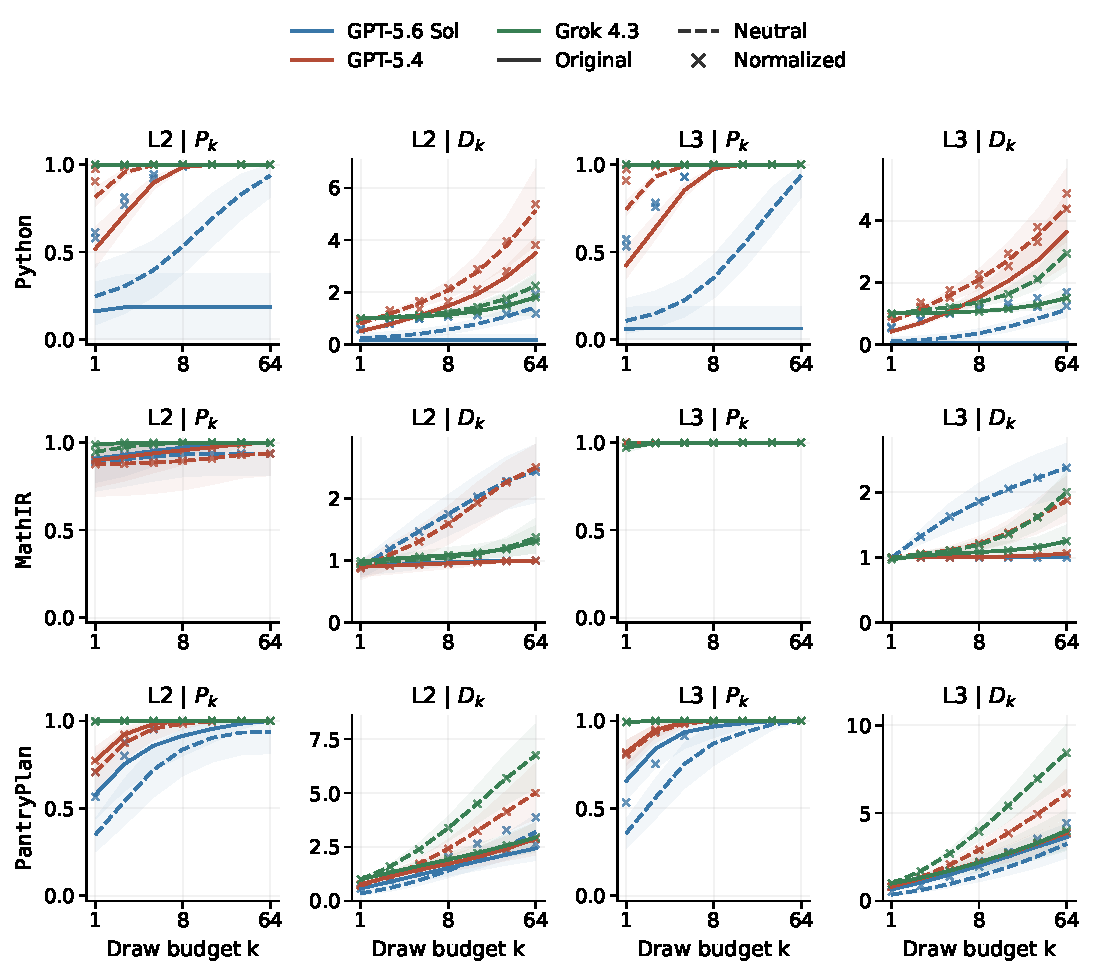
\includegraphics[width=\linewidth,height=0.72\textheight,keepaspectratio]{figures/modebench_discovery_curves_frontier.pdf}

\caption{\textbf{Additional draws reveal solution modes beyond early success.} Hosted deployments; rows show \texttt{Python}, \texttt{MathIR}, and \texttt{PantryPlan}, with paired $P_k$ and $D_k$ columns for Levels~2 and~3. Curves show pass probability $P_k$ and distinct verified modes $D_k$ against draw budget $k$, obtained by averaging over size-$k$ subsets within sixteen 64-draw problem pools per domain and level. Colours identify deployments; solid/dashed lines denote original/neutral wording. Lines use strict verification, crosses formatting normalization, and shading pointwise 95\% bootstrap intervals. Intervals resample paired problems within each domain and level and condition on the deployment.}

\label{fig:discovery-curves-frontier}

\end{figure}

\begin{table}[!htbp]
\centering\scriptsize
\setlength{\tabcolsep}{3pt}
\caption{\textbf{Pair weighting changes the summary of correct-solution diversity.} Strict 64-draw estimates for hosted deployments. Collision $C$ weights prompts by their number of correct pairs; \pmd{} weights eligible prompts equally. Absolute estimates for each wording use their own eligible prompts, whereas $\Delta\pmd$ uses only jointly eligible prompts. Thus $\Delta\pmd$ need not equal the difference between the displayed absolute estimates, and $E_O/E_N$ are separate eligibility counts. Each deployment is fixed; intervals resample paired problems.}
\label{tab:discovery-breadth-frontier}
\resizebox{\linewidth}{!}{%
\begin{tabular}{llrrrrrrrrr}
\toprule
Model & Domain/level & $C_O$ & $C_N$ & $\pmd_O$ & $\pmd_N$ & $U^{C}_O$ & $U^{\pmd}_O$ & $E_O/E_N$ & $Q_O/Q_N$ & $\Delta\pmd$ [95\%] \\
\midrule
GPT-5.4 & \texttt{Python} L2 & $0.790$ & $0.665$ & $0.257$ & $0.341$ & $0.500$ & $0.500$ & 16/16 & 10374/21720 & $+0.084\;[-0.006,+0.186]$ \\
GPT-5.6 Sol & \texttt{Python} L2 & $1.000$ & $0.974$ & $0.000$ & $0.184$ & $0.500$ & $0.500$ & 3/13 & 4467/6074 & $+0.021\;[+0.000,+0.032]$ \\
Grok 4.3 & \texttt{Python} L2 & $0.963$ & $0.938$ & $0.037$ & $0.062$ & $0.500$ & $0.500$ & 16/16 & 32256/32256 & $+0.025\;[+0.002,+0.048]$ \\
GPT-5.4 & \texttt{Python} L3 & $0.732$ & $0.620$ & $0.334$ & $0.384$ & $0.500$ & $0.500$ & 16/16 & 6747/18043 & $+0.050\;[-0.026,+0.128]$ \\
GPT-5.6 Sol & \texttt{Python} L3 & $1.000$ & $0.966$ & $0.000$ & $0.130$ & $0.500$ & $0.500$ & 1/10 & 1953/2097 & $+0.031\;[+0.031,+0.031]$ \\
Grok 4.3 & \texttt{Python} L3 & $0.981$ & $0.893$ & $0.019$ & $0.107$ & $0.500$ & $0.500$ & 16/16 & 32193/32256 & $+0.087\;[+0.041,+0.154]$ \\
GPT-5.4 & \texttt{MathIR} L2 & $1.000$ & $0.756$ & $0.000$ & $0.228$ & $0.200$ & $0.800$ & 16/15 & 28440/28227 & $+0.228\;[+0.161,+0.302]$ \\
GPT-5.6 Sol & \texttt{MathIR} L2 & $1.000$ & $0.678$ & $0.000$ & $0.302$ & $0.200$ & $0.800$ & 16/15 & 28645/28377 & $+0.302\;[+0.200,+0.402]$ \\
Grok 4.3 & \texttt{MathIR} L2 & $0.968$ & $0.985$ & $0.033$ & $0.014$ & $0.200$ & $0.800$ & 16/16 & 31600/29677 & $-0.020\;[-0.076,+0.017]$ \\
GPT-5.4 & \texttt{MathIR} L3 & $0.998$ & $0.944$ & $0.002$ & $0.056$ & $0.200$ & $0.800$ & 16/16 & 32256/32256 & $+0.054\;[+0.027,+0.087]$ \\
GPT-5.6 Sol & \texttt{MathIR} L3 & $1.000$ & $0.676$ & $0.000$ & $0.324$ & $0.200$ & $0.800$ & 16/16 & 32256/32256 & $+0.324\;[+0.208,+0.432]$ \\
Grok 4.3 & \texttt{MathIR} L3 & $0.966$ & $0.949$ & $0.033$ & $0.051$ & $0.200$ & $0.800$ & 16/16 & 30520/32193 & $+0.019\;[-0.046,+0.064]$ \\
GPT-5.4 & \texttt{PantryPlan} L2 & $0.680$ & $0.499$ & $0.252$ & $0.483$ & $0.069$ & $0.934$ & 16/16 & 20097/17436 & $+0.231\;[+0.069,+0.395]$ \\
GPT-5.6 Sol & \texttt{PantryPlan} L2 & $0.674$ & $0.624$ & $0.275$ & $0.474$ & $0.076$ & $0.934$ & 16/15 & 12941/5001 & $+0.180\;[+0.058,+0.327]$ \\
Grok 4.3 & \texttt{PantryPlan} L2 & $0.684$ & $0.412$ & $0.315$ & $0.589$ & $0.066$ & $0.934$ & 16/16 & 32005/32193 & $+0.274\;[+0.143,+0.411]$ \\
GPT-5.4 & \texttt{PantryPlan} L3 & $0.546$ & $0.392$ & $0.431$ & $0.610$ & $0.065$ & $0.937$ & 16/16 & 22332/21975 & $+0.179\;[+0.103,+0.257]$ \\
GPT-5.6 Sol & \texttt{PantryPlan} L3 & $0.566$ & $0.652$ & $0.422$ & $0.441$ & $0.061$ & $0.937$ & 16/16 & 15229/4946 & $+0.019\;[-0.136,+0.172]$ \\
Grok 4.3 & \texttt{PantryPlan} L3 & $0.673$ & $0.294$ & $0.330$ & $0.703$ & $0.063$ & $0.937$ & 16/16 & 31830/31881 & $+0.373\;[+0.224,+0.523]$ \\
\bottomrule
\end{tabular}}
\end{table}

\begin{figure}[!htbp]

\centering

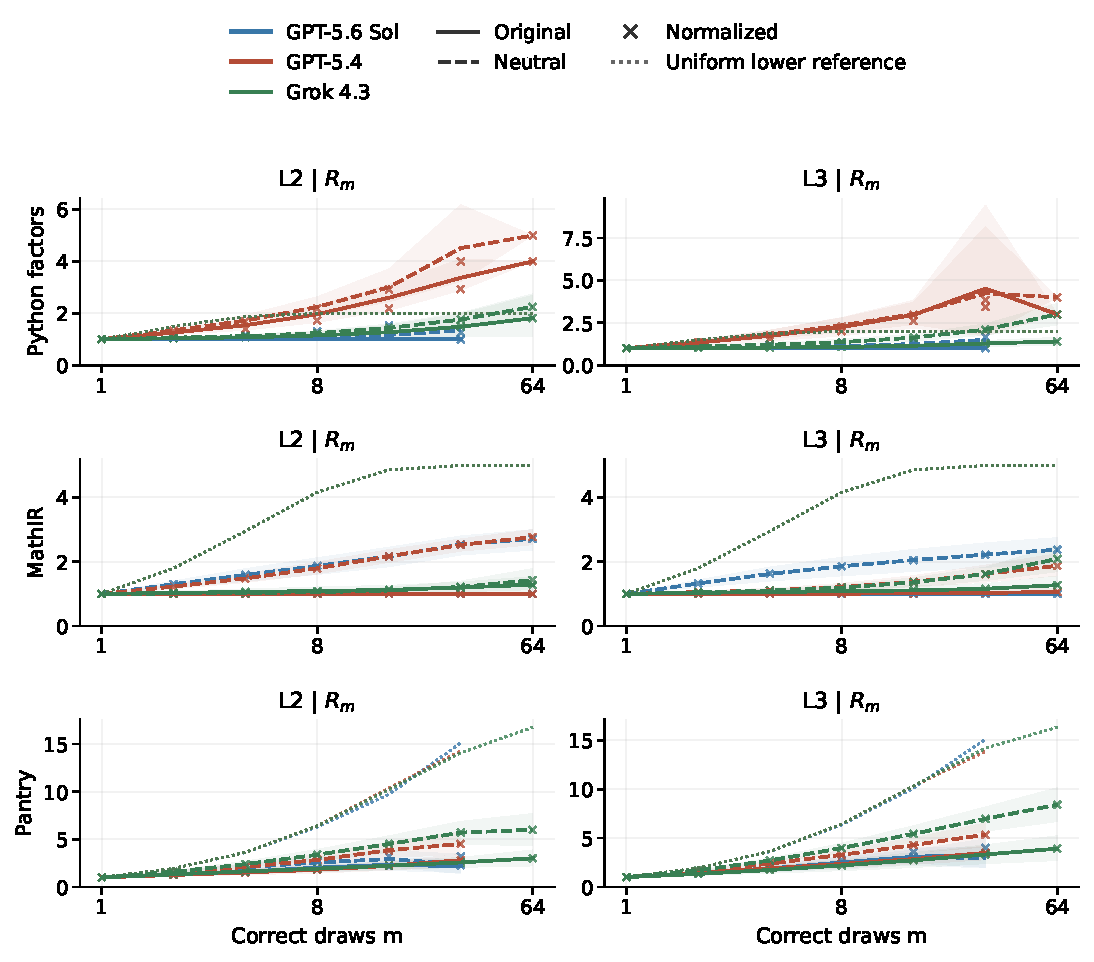
\includegraphics[width=\linewidth,height=0.66\textheight,keepaspectratio]{figures/modebench_discovery_correct_budget_frontier.pdf}

\caption{\textbf{Neutral wording broadens GPT solutions in \texttt{MathIR} at fixed correct-draw budgets.} Hosted deployments; rows show \texttt{Python}, \texttt{MathIR}, and \texttt{PantryPlan}, and columns Levels~2 and~3. Curves show $R_m$, the expected number of distinct verified modes in $m$ correct draws, on prompts with at least $m$ correct outputs under both wordings. Eligibility varies with $m$, method, and grading; gaps mark undefined means. Dotted lines give uniform lower references on prompts eligible under strict grading in both wordings, with the same prompt and checkpoint weighting as the strict curves. Colours identify deployments; solid/dashed lines denote original/neutral wording. Lines use strict verification, crosses formatting normalization, and shading pointwise 95\% bootstrap intervals. Intervals resample paired problems within each domain and level and condition on the deployment.}

\label{fig:discovery-correct-budget-frontier}

\end{figure}

\begin{table}[!htbp]
\centering\scriptsize
\setlength{\tabcolsep}{3pt}
\caption{\textbf{Discovery gains from eight to 64 draws.} Strict verification; O/N denotes original/neutral wording. Qwen2.5-0.5B-Instruct checkpoint means use five training seeds in \texttt{Python} and \texttt{MathIR} and two in \texttt{PantryPlan}; $s=1$ denotes the single initial checkpoint. Five-seed intervals resample seeds and paired prompts; \texttt{PantryPlan} intervals condition on its two checkpoints. Formatting normalization leaves every Qwen estimate unchanged.}
\label{tab:discovery-gains-local-strict}
\resizebox{\linewidth}{!}{%
\begin{tabular}{llrrrr}
\toprule
Model & Domain/level & $G_P$: O/N & $G_D$: O/N & $G_B$: O/N & $\Delta G_D$ [95\%] \\
\midrule
Dr.GRPO ($s=5$) & \texttt{Python} L2 & $0.000/0.000$ & $0.000/0.000$ & $0.000/0.000$ & $+0.000\;[+0.000,+0.000]$ \\
Initial ($s=1$) & \texttt{Python} L2 & $0.147/0.105$ & $0.303/0.165$ & $0.156/0.060$ & $-0.138\;[-0.217,-0.061]$ \\
Re:Dr ($s=5$) & \texttt{Python} L2 & $0.000/0.231$ & $0.058/0.463$ & $0.058/0.232$ & $+0.405\;[+0.185,+0.620]$ \\
Dr.GRPO ($s=5$) & \texttt{Python} L3 & $0.000/0.033$ & $0.000/0.033$ & $0.000/0.000$ & $+0.033\;[+0.000,+0.120]$ \\
Initial ($s=1$) & \texttt{Python} L3 & $0.218/0.096$ & $0.593/0.096$ & $0.376/0.000$ & $-0.497\;[-0.766,-0.270]$ \\
Re:Dr ($s=5$) & \texttt{Python} L3 & $0.000/0.239$ & $0.153/0.531$ & $0.153/0.292$ & $+0.379\;[+0.111,+0.678]$ \\
Dr.GRPO ($s=5$) & \texttt{MathIR} L2 & $0.021/0.017$ & $0.021/0.017$ & $0.000/0.000$ & $-0.004\;[-0.068,+0.045]$ \\
Initial ($s=1$) & \texttt{MathIR} L2 & $0.344/0.235$ & $0.344/0.235$ & $0.000/0.000$ & $-0.109\;[-0.383,+0.164]$ \\
Re:Dr ($s=5$) & \texttt{MathIR} L2 & $0.010/0.011$ & $0.010/0.011$ & $0.000/0.000$ & $+0.001\;[-0.036,+0.050]$ \\
Dr.GRPO ($s=5$) & \texttt{MathIR} L3 & $0.023/0.018$ & $0.026/0.018$ & $0.004/0.000$ & $-0.008\;[-0.065,+0.038]$ \\
Initial ($s=1$) & \texttt{MathIR} L3 & $0.254/0.246$ & $0.359/0.360$ & $0.105/0.114$ & $+0.001\;[-0.123,+0.095]$ \\
Re:Dr ($s=5$) & \texttt{MathIR} L3 & $0.064/0.056$ & $0.064/0.056$ & $0.000/0.000$ & $-0.008\;[-0.099,+0.059]$ \\
Dr.GRPO ($s=2$) & \texttt{PantryPlan} L2 & $0.332/0.323$ & $0.718/0.736$ & $0.386/0.414$ & $+0.018\;[-0.422,+0.433]$ \\
Initial ($s=1$) & \texttt{PantryPlan} L2 & $0.440/0.419$ & $0.857/0.955$ & $0.416/0.537$ & $+0.099\;[-0.201,+0.392]$ \\
Re:Dr ($s=2$) & \texttt{PantryPlan} L2 & $0.141/0.147$ & $0.415/0.429$ & $0.274/0.282$ & $+0.014\;[-0.123,+0.152]$ \\
Dr.GRPO ($s=2$) & \texttt{PantryPlan} L3 & $0.268/0.258$ & $0.949/1.025$ & $0.681/0.766$ & $+0.076\;[-0.237,+0.465]$ \\
Initial ($s=1$) & \texttt{PantryPlan} L3 & $0.259/0.384$ & $0.927/1.078$ & $0.668/0.694$ & $+0.151\;[-0.109,+0.399]$ \\
Re:Dr ($s=2$) & \texttt{PantryPlan} L3 & $0.204/0.149$ & $0.568/0.461$ & $0.364/0.312$ & $-0.107\;[-0.321,+0.098]$ \\
\bottomrule
\end{tabular}}
\end{table}

\begin{figure}[!htbp]

\centering

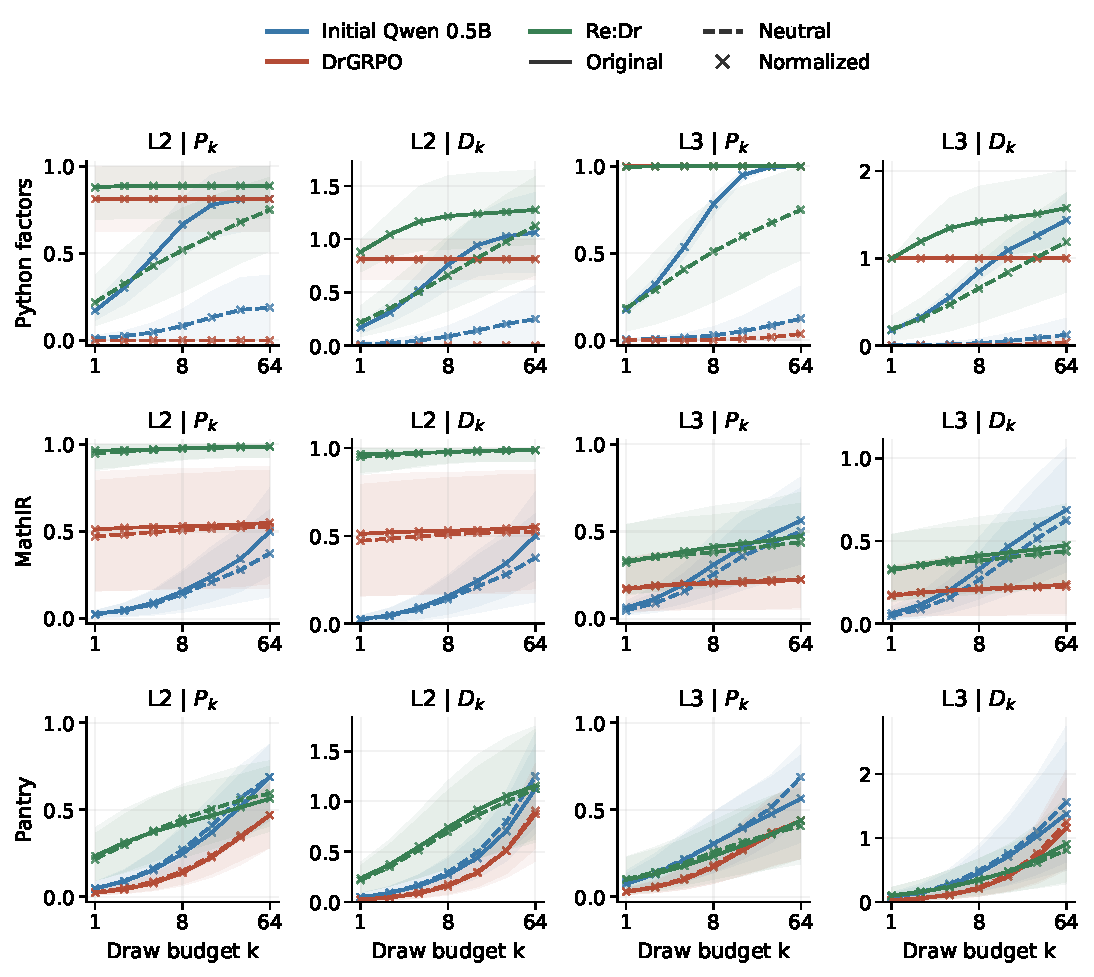
\includegraphics[width=\linewidth,height=0.72\textheight,keepaspectratio]{figures/modebench_discovery_curves_local.pdf}

\caption{\textbf{Additional draws reveal few new \texttt{MathIR} modes after training.} Qwen2.5-0.5B-Instruct checkpoints; rows show \texttt{Python}, \texttt{MathIR}, and \texttt{PantryPlan}, with paired $P_k$ and $D_k$ columns for Levels~2 and~3. Curves show pass probability $P_k$ and distinct verified modes $D_k$ against draw budget $k$, obtained by averaging over size-$k$ subsets within sixteen 64-draw problem pools per domain and level. Colours identify methods; solid/dashed lines denote original/neutral wording. Lines use strict verification, crosses formatting normalization, and shading pointwise 95\% bootstrap intervals. Means weight checkpoints equally: five training seeds in \texttt{Python} and \texttt{MathIR}, two in \texttt{PantryPlan}, and one initial checkpoint. Five-seed intervals resample seeds and paired problems; \texttt{PantryPlan} and initial intervals condition on the observed checkpoints for each method.}

\label{fig:discovery-curves-local}

\end{figure}

\begin{table}[!htbp]
\centering\scriptsize
\setlength{\tabcolsep}{3pt}
\caption{\textbf{Pair weighting changes the summary of correct-solution diversity.} Strict 64-draw estimates for Qwen2.5-0.5B-Instruct checkpoints. Collision $C$ weights prompts by their number of correct pairs; \pmd{} weights eligible prompts equally. Absolute estimates for each wording use their own eligible prompts, whereas $\Delta\pmd$ uses only jointly eligible prompts. Thus $\Delta\pmd$ need not equal the difference between the displayed absolute estimates, and $E_O/E_N$ are separate eligibility counts. Means weight checkpoints equally and are undefined if any seed lacks eligible prompts.}
\label{tab:discovery-breadth-local}
\resizebox{\linewidth}{!}{%
\begin{tabular}{llrrrrrrrrr}
\toprule
Model & Domain/level & $C_O$ & $C_N$ & $\pmd_O$ & $\pmd_N$ & $U^{C}_O$ & $U^{\pmd}_O$ & $E_O/E_N$ & $Q_O/Q_N$ & $\Delta\pmd$ [95\%] \\
\midrule
Dr.GRPO & \texttt{Python} L2 & $1.000$ & $--$ & $0.000$ & $--$ & $0.500$ & $0.500$ & 65/0 & 130977/0 & $--$ \\
Initial & \texttt{Python} L2 & $0.791$ & $0.875$ & $0.097$ & $0.167$ & $0.500$ & $0.500$ & 13/3 & 1270/24 & $-0.252\;[-0.395,+0.019]$ \\
Re:Dr & \texttt{Python} L2 & $0.809$ & $0.800$ & $0.191$ & $0.156$ & $0.500$ & $0.500$ & 71/53 & 140722/18289 & $-0.037\;[-0.139,+0.037]$ \\
Dr.GRPO & \texttt{Python} L3 & $1.000$ & $--$ & $0.000$ & $--$ & $0.500$ & $0.500$ & 80/0 & 161280/0 & $--$ \\
Initial & \texttt{Python} L3 & $0.875$ & $1.000$ & $0.101$ & $0.000$ & $0.500$ & $0.500$ & 16/1 & 1010/3 & $-0.513\;[-0.513,-0.513]$ \\
Re:Dr & \texttt{Python} L3 & $0.805$ & $0.797$ & $0.195$ & $0.227$ & $0.500$ & $0.500$ & 80/52 & 160275/12893 & $+0.030\;[-0.023,+0.117]$ \\
Dr.GRPO & \texttt{MathIR} L2 & $1.000$ & $1.000$ & $0.000$ & $0.000$ & $0.200$ & $0.800$ & 43/42 & 80766/74119 & $+0.000\;[+0.000,+0.000]$ \\
Initial & \texttt{MathIR} L2 & $1.000$ & $1.000$ & $0.000$ & $0.000$ & $0.200$ & $0.800$ & 3/3 & 64/64 & $+0.000\;[+0.000,+0.000]$ \\
Re:Dr & \texttt{MathIR} L2 & $1.000$ & $1.000$ & $0.000$ & $0.000$ & $0.200$ & $0.800$ & 79/79 & 155016/151485 & $+0.000\;[+0.000,+0.000]$ \\
Dr.GRPO & \texttt{MathIR} L3 & $0.980$ & $1.000$ & $0.038$ & $0.000$ & $0.200$ & $0.800$ & 16/18 & 24457/25393 & $-0.038\;[-0.202,+0.000]$ \\
Initial & \texttt{MathIR} L3 & $0.883$ & $0.912$ & $0.128$ & $0.162$ & $0.200$ & $0.800$ & 7/6 & 282/181 & $+0.013\;[-0.014,+0.052]$ \\
Re:Dr & \texttt{MathIR} L3 & $1.000$ & $1.000$ & $0.000$ & $0.000$ & $0.200$ & $0.800$ & 34/34 & 46891/50301 & $+0.000\;[+0.000,+0.000]$ \\
Dr.GRPO & \texttt{PantryPlan} L2 & $0.374$ & $0.276$ & $0.733$ & $0.780$ & $0.047$ & $0.953$ & 9/10 & 101/193 & $+0.220\;[-0.030,+0.470]$ \\
Initial & \texttt{PantryPlan} L2 & $0.849$ & $0.787$ & $0.587$ & $0.623$ & $0.052$ & $0.945$ & 7/10 & 212/178 & $-0.078\;[-0.300,+0.064]$ \\
Re:Dr & \texttt{PantryPlan} L2 & $0.600$ & $0.613$ & $0.343$ & $0.218$ & $0.051$ & $0.942$ & 16/18 & 10144/8510 & $-0.093\;[-0.220,+0.007]$ \\
Dr.GRPO & \texttt{PantryPlan} L3 & $0.203$ & $0.228$ & $0.808$ & $0.680$ & $0.047$ & $0.950$ & 10/12 & 134/165 & $-0.156\;[-0.359,+0.081]$ \\
Initial & \texttt{PantryPlan} L3 & $0.375$ & $0.313$ & $0.307$ & $0.341$ & $0.049$ & $0.945$ & 7/6 & 531/705 & $-0.017\;[-0.109,+0.091]$ \\
Re:Dr & \texttt{PantryPlan} L3 & $0.636$ & $0.666$ & $0.337$ & $0.198$ & $0.051$ & $0.941$ & 10/11 & 4006/3946 & $-0.112\;[-0.319,+0.008]$ \\
\bottomrule
\end{tabular}}
\end{table}

\begin{figure}[!htbp]

\centering

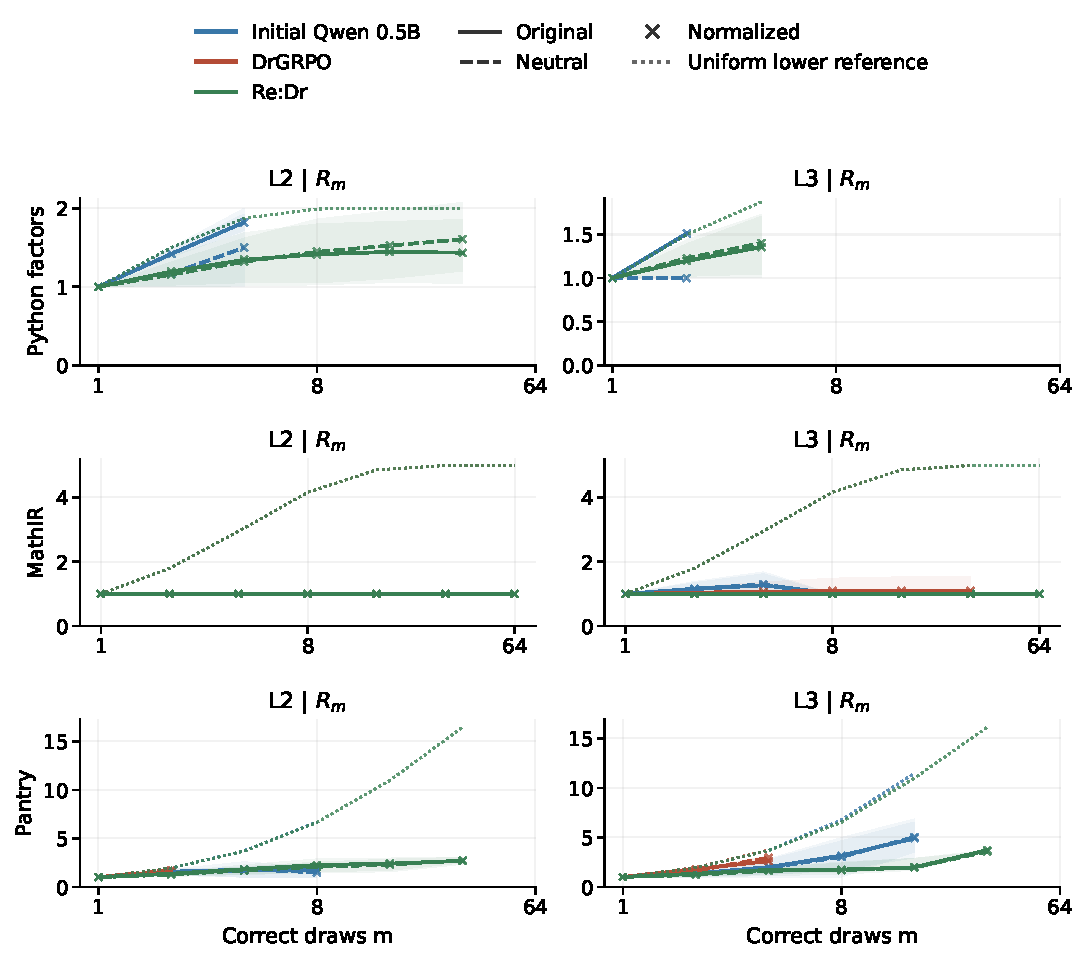
\includegraphics[width=\linewidth,height=0.66\textheight,keepaspectratio]{figures/modebench_discovery_correct_budget_local.pdf}

\caption{\textbf{\texttt{MathIR} correct solutions remain concentrated after training.} Qwen2.5-0.5B-Instruct checkpoints; rows show \texttt{Python}, \texttt{MathIR}, and \texttt{PantryPlan}, and columns Levels~2 and~3. Curves show $R_m$, the expected number of distinct verified modes in $m$ correct draws, on prompts with at least $m$ correct outputs under both wordings. Eligibility varies with $m$, method, and grading; gaps mark undefined means. Dotted lines give uniform lower references on prompts eligible under strict grading in both wordings, with the same prompt and checkpoint weighting as the strict curves. Colours identify methods; solid/dashed lines denote original/neutral wording. Lines use strict verification, crosses formatting normalization, and shading pointwise 95\% bootstrap intervals. Means weight checkpoints equally: five training seeds in \texttt{Python} and \texttt{MathIR}, two in \texttt{PantryPlan}, and one initial checkpoint. Five-seed intervals resample seeds and paired problems; \texttt{PantryPlan} and initial intervals condition on the observed checkpoints for each method.}

\label{fig:discovery-correct-budget-local}

\end{figure}


\subsection{Hosted-model discovery: wording, formatting, and additional draws}
\label{app:hosted-discovery-complete}

The hosted evaluation contains 36,864 responses from GPT-5.4, GPT-5.6 Sol,
and Grok 4.3. Each deployment receives sixteen problems from each of
\texttt{Python}, \texttt{MathIR}, and \texttt{PantryPlan} at Levels~2 and~3,
with two wordings and 64 draws per wording. All three deployments use
medium reasoning effort and an 8,192-token output cap. These settings
differ from the reasoning-disabled main-table evaluation. The \texttt{Python}
comparisons use the same mathematical problems under both wordings.
The hosted models receive no task-specific training in this evaluation.

\paragraph{Neutral wording broadens the GPT models' correct \texttt{MathIR} solutions.}
Both GPT deployments yield at most one verified mode per Level-2 problem
in 64 original-wording draws. Among problems with
at least eight correct responses under both wordings, neutral wording
increases mean breadth at eight correct draws by $.794$ ($[.623,.990]$)
for GPT-5.4 and $.872$ ($[.606,1.123]$) for GPT-5.6 Sol.
The Level-3 effects are $.204$ ($[.106,.320]$) and $.860$
($[.563,1.141]$). These comparisons include fourteen and fifteen jointly
eligible problems at Level~2, respectively, and sixteen for each GPT
deployment at Level~3. Grok 4.3's corresponding intervals include zero at
both levels.

The pointwise intervals resample the sixteen paired problems
within each domain and level, conditioning on the deployment. They do not
include variation across model training seeds. These breadth contrasts
describe jointly eligible problems without equating the wordings' accuracy.

\paragraph{Additional draws reveal more \texttt{PantryPlan} modes after first success.}
Under neutral wording, GPT-5.4 gains $2.583$ and $3.219$ verified modes
between eight and 64 draws at Levels~2 and~3; Grok 4.3 gains $3.377$ and
$4.466$. Grok 4.3's empirical pass probability is already $1.0$ at eight draws
at both levels, so these gains consist entirely of additional modes.
At Level~3 its distinct count rises from $3.972$ to $8.438$.
On jointly eligible problems at eight correct draws, neutral minus
original breadth is $1.781$ ($[1.226,2.338]$) for Grok 4.3 and $.934$
($[.670,1.184]$) for GPT-5.4; GPT-5.6 Sol's Level-3 contrast is
inconclusive. These counts measure finite-sample discovery rather than
exhaustive solution coverage.

\paragraph{Formatting limits GPT-5.6 Sol's strict \texttt{Python} scores.}
GPT-5.6 Sol's original-wording strict pass probability is approximately
$.1875$ at Level~2 and $.0625$ at Level~3 from eight through 64 draws.
Formatting normalization gives $P_{64}=1.0$ under both wordings at both
levels, with all four $P_8$ values above $.989$. The low strict scores
therefore include failures to express valid solutions in the required
format.

After normalization, the neutral-minus-original difference in
discovery gains from eight to 64 draws is $.681$ ($[.351,1.066]$) at Level~2 and $.370$
($[.112,.674]$) at Level~3. Normalization changes response formatting
before applying the same verifier and canonical-key extraction rules.


% Generated by ops/build_paper_gpt56_all_levels32_discovery.py; do not edit.
\subsection{All five domains and all three levels at 512 draws}
\label{app:gpt56-all-levels-discovery}

We evaluate GPT-5.6 Sol on thirty-two problems from each of five domains
at Levels~1, 2, and~3, using the original prompt wording. Problems are
selected independently of model outputs.
Each problem receives 512 responses: 480 problems and 245,760
responses in total. Requests use medium reasoning, an 8,192-token output
limit, and unspecified temperature and top-$p$, with model snapshot
\texttt{gpt-5.6-sol-2026-07-09}. Invalid, refused, and truncated answers remain in the sampling denominator.

Figure~\ref{fig:gpt56-sampling-budget} uses formatting-normalized grading;
Table~\ref{tab:gpt56-all-levels-endpoints} also gives strict-verifier results
on the same response pools. In draw-index order, the first 64 responses
solve 474 of 480 problems after normalization and 418 under strict grading.
At 512 responses, these counts are 477 and 436, respectively.

For a pool of $N=512$ responses, with $c$ correct responses and verified-mode counts $n_j$,
success probability and expected distinct modes in a uniformly sampled $k$-subset are
\[
 P_N(k)=1-\frac{\binom{N-c}{k}}{\binom Nk},\qquad
 D_N(k)=\sum_j\left[1-\frac{\binom{N-n_j}{k}}{\binom Nk}\right],
\]
respectively. We average all thirty-two problems equally within each
domain and level, including problems with no correct response.
Every curve uses the complete 512-response pools at budgets
$k\in\{1,2,4,8,16,32,64,128,256,512\}$. The rarefied estimate at $k=64$
need not equal the result from the first 64 responses in draw-index order.
The gain from the final budget doubling is $D_{512}(512)-D_{512}(256)$.
Pointwise 95\% intervals use 20,000 whole-problem bootstrap replicates
within domain and level; the same resampled problems
form both sides of each contrast. Intervals do not provide simultaneous
coverage across budgets, domains, or levels.

\begin{table}[!htbp]
  \centering
  \footnotesize
  \setlength{\tabcolsep}{4pt}
  \resizebox{\linewidth}{!}{%
  \begin{tabular}{llrrrrr}
    \toprule
    & & & \multicolumn{2}{c}{$D/P$ at 512} & \multicolumn{2}{c}{$\Delta D$, 256 to 512 [95\% CI]} \\
    \cmidrule(lr){4-5}\cmidrule(l){6-7}
    Domain & Level & Known support (range) & Normalized & Strict & Normalized & Strict \\
    \midrule
    \texttt{Graph} & 1 & $6.97$ (4--12) & 2.531/100.0 & 2.531/100.0 & 0.222 [0.142, 0.305] & 0.222 [0.142, 0.305] \\
    \texttt{Graph} & 2 & $6.03$ (4--12) & 2.625/100.0 & 2.625/100.0 & 0.268 [0.170, 0.373] & 0.268 [0.170, 0.373] \\
    \texttt{Graph} & 3 & $6.66$ (4--12) & 1.719/100.0 & 1.719/100.0 & 0.137 [0.059, 0.228] & 0.137 [0.059, 0.228] \\
    \addlinespace[2pt]
    \texttt{Countdown} & 1 & $\geq 4.53$ (2--6) & 3.469/100.0 & 3.375/100.0 & 0.148 [0.070, 0.243] & 0.164 [0.083, 0.259] \\
    \texttt{Countdown} & 2 & $\geq 4.40$ (3--7) & 3.156/100.0 & 3.094/100.0 & 0.218 [0.123, 0.320] & 0.235 [0.136, 0.344] \\
    \texttt{Countdown} & 3 & $\geq 4.25$ (2--8) & 2.812/100.0 & 2.562/100.0 & 0.181 [0.090, 0.289] & 0.191 [0.097, 0.297] \\
    \addlinespace[2pt]
    \texttt{Python} & 1 & $\geq 2.00$ (2) & 3.750/100.0 & 2.875/100.0 & 0.592 [0.438, 0.750] & 0.492 [0.334, 0.656] \\
    \texttt{Python} & 2 & $\geq 2.00$ (2) & 1.438/100.0 & 0.562/43.8 & 0.073 [0.020, 0.135] & 0.148 [0.078, 0.227] \\
    \texttt{Python} & 3 & $\geq 2.00$ (2) & 1.344/100.0 & 0.281/28.1 & 0.013 [0.000, 0.032] & 0.086 [0.031, 0.156] \\
    \addlinespace[2pt]
    \texttt{MathIR} & 1 & $\geq 5.00$ (5) & 1.906/93.8 & 1.906/93.8 & 0.071 [0.012, 0.153] & 0.071 [0.012, 0.153] \\
    \texttt{MathIR} & 2 & $\geq 5.00$ (5) & 1.000/100.0 & 1.000/100.0 & 0.002 [0.000, 0.006] & 0.002 [0.000, 0.006] \\
    \texttt{MathIR} & 3 & $\geq 5.00$ (5) & 0.969/96.9 & 0.969/96.9 & 0.000 [0.000, 0.000] & 0.000 [0.000, 0.000] \\
    \addlinespace[2pt]
    \texttt{PantryPlan} & 1 & $\geq 16.90$ (8--39) & 6.906/100.0 & 6.906/100.0 & 0.622 [0.458, 0.799] & 0.622 [0.458, 0.799] \\
    \texttt{PantryPlan} & 2 & $\geq 16.50$ (8--39) & 4.875/100.0 & 4.625/100.0 & 0.702 [0.476, 0.951] & 0.702 [0.472, 0.962] \\
    \texttt{PantryPlan} & 3 & $\geq 16.87$ (8--40) & 5.562/100.0 & 5.250/100.0 & 0.719 [0.527, 0.914] & 0.678 [0.489, 0.875] \\
    \bottomrule
  \end{tabular}
  }
  \caption{\textbf{Late mode discovery is largest in \texttt{PantryPlan} and Level-1 \texttt{Python}.}
  GPT-5.6 Sol with original wording and 512 responses for each of thirty-two
  problems per domain and level. $D/P$ gives mean distinct verified modes
  and the percentage of problems solved at least once.
  Support gives the mean and range within each domain and level: exact for \texttt{Graph} and a certified
  lower bound elsewhere. Strict and normalized grading use identical pools.
  The paired contrast $\Delta D=D_{512}(512)-D_{512}(256)$ measures the gain
  in expected distinct modes between random subsets of the complete pool, rather than between successive draws.
  Brackets give pointwise 95\% whole-problem bootstrap intervals.}
  \label{tab:gpt56-all-levels-endpoints}
\end{table}

The \texttt{Graph} support count includes every assignment compatible with the fixed colors.
\texttt{Countdown} references enumerate binary expression trees; the validator
also accepts unary negation and retains it in canonical keys, so these
counts are lower bounds. The \texttt{Python}, \texttt{MathIR}, and \texttt{PantryPlan} references
are also certified lower bounds. Exceeding a lower bound does not imply
that all available modes have been discovered.

Figure~\ref{fig:gpt56-sampling-budget} divides the mean distinct-mode count
by the mean enumerated mode count for the same thirty-two problems.
This ratio of means differs from the mean fraction of modes recovered per
problem; the denominator is held fixed when scaling interval endpoints.
The independently certified references in Table~\ref{tab:gpt56-all-levels-endpoints}
can be smaller than these enumerated counts. In \texttt{Python}, the table certifies
at least two modes per problem, while the mean enumerated counts used
in the figure are 222, 335.75, and 354.75 at Levels~1, 2, and~3.

These curves describe random subsets of the observed response pools.
Using them to predict discovery from new responses at each budget also
requires stable sampling behavior across requests; a common model snapshot
and decoding settings do not ensure this. Small or zero gains at the
largest budgets do not rule out rare unseen modes.


\subsection{Discovery at larger sampling budgets}
\label{app:sampling-budget-effects}

The 64-draw comparison in App.~\ref{app:sampling-budget-ablation} uses
36,864 responses from hosted models and 110,592 from Qwen checkpoints,
147,456 in total. Each of the six hosted model--wording combinations
contributes 6,144 responses. The Qwen evaluation includes 25 checkpoints:
each trained checkpoint is evaluated in its training domain at Levels~2
and~3, and the initial checkpoint covers all six domain--level combinations.
Every response remains in its sampling denominator. Formatting normalization
adds no verified Qwen responses, so both grading rules yield identical
estimates for these checkpoints. The sixteen problems per domain and level
differ from the thirty-two used in the 512-draw study
(App.~\ref{app:gpt56-all-levels-discovery}).

\paragraph{Prompt weighting changes the diversity summary.}
Tables~\ref{tab:discovery-breadth-frontier} and~\ref{tab:discovery-breadth-local}
compare two summaries of the 64-response pools. Within each checkpoint or
deployment, collision $C$ pools correct pairs across prompts, weighting each
prompt in proportion to $\binom{c}{2}$. Promptwise \pmd{} gives equal weight
to each prompt with at least two verified responses. Trained-checkpoint
scores then receive equal weight across seeds. Across 70 defined
combinations of model, domain, level, and wording, the median absolute
difference between promptwise \pmd{} and $1-C$ is $.003$, but nineteen
differ by at least $.05$.

For the initial checkpoint under original wording,
Level-2 \texttt{PantryPlan} has $1-C=.151$ and promptwise \pmd{} of $.587$;
Level~3 has $.625$ and $.307$, respectively. Both estimates use seven of
sixteen problems. The direction of the difference depends on which prompts
supply the most correct pairs and therefore receive the largest weights.

Neither weighting holds overall accuracy or the eligible population fixed.
For the initial checkpoint, Level-3 \texttt{Python} has sixteen eligible
problems under original wording and one under neutral wording. Each wording's
absolute estimate uses its own eligible prompts; paired differences use
only jointly eligible prompts. Equal prompt weights therefore describe
conditional diversity within these selected populations
(App.~\ref{app:metric-sampling}).

\paragraph{\texttt{MathIR}: concentration largely persists through 64 draws.}
At Level~2, both trained methods have $B_k=0$ at every measured budget under
both wordings. Re:Dr has $P_8=.9774$ and $P_{64}=.9875$ under original
wording, compared with $.9767$ and $.9875$ under neutral wording. Its $D_k$
equals $P_k$ throughout, so the small increase comes entirely from first
successes. At a budget of eight correct draws, both wordings have $R_8=1$
on the same 76 eligible checkpoint--problem pairs, compared with the
uniform lower reference $5[1-(4/5)^8]=4.1611$ from certified support.
These pairs reuse the same 16 problems across five checkpoints.

At Level~3, both trained methods under neutral wording and Re:Dr under
original wording also yield at most one correct key per checkpoint and
problem. Dr.GRPO under original wording has one exception: one checkpoint--problem
pair contains two keys with counts 28 and 9. Averaging over seeds and problems
gives $B_{64}=.0125$ and $B_{64}-B_8=.0035$. The corresponding equal-seed
correct-pair collision is $.9803$; the other trained \texttt{MathIR}
conditions have collision $1.0$, against the uniform upper reference $.2$.
The larger budget thus reveals a rare additional mode, precluding an exact
single-mode description of every trained condition.

\paragraph{\texttt{Python}: prompt dependence and additional discovery coexist.}
Under original wording, Dr.GRPO has $P_k=D_k=.8125$ at Level~2 and $1.0$
at Level~3 throughout the range from eight to 64 draws. Under neutral wording,
it has zero correct responses out of 5,120 at Level~2 and three out of
5,120 at Level~3. Each success is the only correct response for its
checkpoint--problem pair. The Level~3 mean is therefore
$P_{64}=D_{64}=.0375$, while correct-pair collision remains undefined.

For Re:Dr under original wording, pass probability is unchanged from eight
to 64 draws, but $D_k$ increases by $.0582$ at Level~2 and $.1529$ at
Level~3. Under neutral wording, $P_k$ rises from $.5186$ to $.7500$ and
from $.5109$ to $.7500$, respectively; $D_k$ rises from $.6618$ to $1.1250$
and from $.6561$ to $1.1875$. These final mode counts remain below the
original-wording values of $1.2750$ and $1.5750$. The corresponding gains
in modes beyond the first success are $.2318$ [$.0574,.4565$] and $.2923$
[$.0659,.5445$], with intervals that resample seeds and paired problems.
Larger budgets therefore recover both first successes and additional
verified alternatives for Re:Dr under neutral wording. These unconditional
gains alone do not identify a change in the conditional distribution of
correct solutions.

\paragraph{\texttt{PantryPlan}: eight draws understate observed discovery.}
Across trained checkpoints at both levels and under both wordings,
$D_{64}-D_8$ ranges from $.4151$ to $1.0247$, with gains in modes beyond
the first success ranging from $.2739$ to $.7664$. The initial checkpoint
also gains $.8565$--$1.0778$ modes. For the two observed training seeds,
the Level~3 method ordering changes with the sampling budget. Under original
wording, Dr.GRPO/Re:Dr have $D_8=.2075/.3381$ but
$D_{64}=1.1563/.9063$; neutral wording gives $.2253/.3515$ at eight draws
and $1.2500/.8125$ at 64. These rankings describe the observed checkpoints
and do not establish a population-level method advantage.

\texttt{PantryPlan} has only two training seeds. Comparisons at larger
correct-draw budgets $m$ often have few or no jointly eligible problems.
They condition on observed success, and the equal-seed mean is undefined
when either seed has no eligible problem.

Several trained conditions remain concentrated at 64 draws, while others
continue to yield additional solution modes. A flat curve over a finite
response pool still leaves open the possibility of rare unseen modes.
Here the $k=8$ points average subsets of sixteen 64-response pools per
domain and level; App.~\ref{app:prompt-hint-ablation} uses a separate
eight-draw evaluation on thirty-two problems per domain and level.
The checkpoints are trained at Level~2, so Level~3 results measure transfer;
hosted results describe fixed deployments.


% Concise theory for both papers; full derivations are preserved in
% paper/audits/streamlining_20260911/full_theory.tex.

% Generated by ops/build_paper_inference_followups.py; do not edit numbers.
\section{Inference: Adaptation, Model Mixtures, and Coarser Keys}
\label{app:inference-followups}
We evaluate adaptation to changed requirements, complementarity between
models, and sensitivity to the definition of a solution mode. Model weights
remain fixed during inference. Pointwise 95\% percentile intervals use 20,000
paired whole-problem bootstrap replicates. Resampling preserves all
perturbations, model conditions, and training seeds for each problem;
hosted comparisons resample within each domain and level. These intervals
condition on the observed response pools and training seeds, so they do not
estimate variability across new response pools or training seeds. The 21
model-pair comparisons are dependent, and intervals are unadjusted for
multiple comparisons.

\subsection{\texttt{PantryPlan} portfolios under changed requirements}
\label{app:pantry-adaptation}
We evaluate the initial Qwen2.5-0.5B checkpoint and Level-2 Dr.GRPO and
Re:Dr checkpoints from two matched training seeds on 32 held-out problems.
We derive 192 single-ingredient outages from the task specifications,
independently of generated answers. Exhaustive search over the original
quantity grid finds valid plans for 181 revised tasks. These plans establish
feasibility and are withheld from the model. Five feasible additional dietary
restrictions are reported separately, as they cover only five source problems.

Each portfolio contains eight plans, which we test unchanged against the
revised requirements. If none remains valid, we allow up to eight sequential
recovery calls and stop at the first valid plan. Unresolved portfolios use
all eight calls. Each recovery prompt contains the revised task, initial
portfolio, previous recovery outputs, and deterministic verifier feedback.
Cumulative success includes portfolios that require no recovery. We average
over perturbations within each source problem, then weight problems equally.

The three sampling strategies use the same checkpoints, verifier, and
192-token response cap. Ordinary sampling uses temperature 1.0. Temperature
tuning selects from $\{0.7,1.0,1.3\}$ based on outage survival on 16 separate
development problems (384 responses per checkpoint). Diversity prompting
makes eight sequential calls, requesting a plan with a new ingredient support
and retaining the complete output history, including failures. All strategies
use the same number of initial responses, but their context lengths and total
token costs differ.

\begin{figure}[!htbp]
\centering
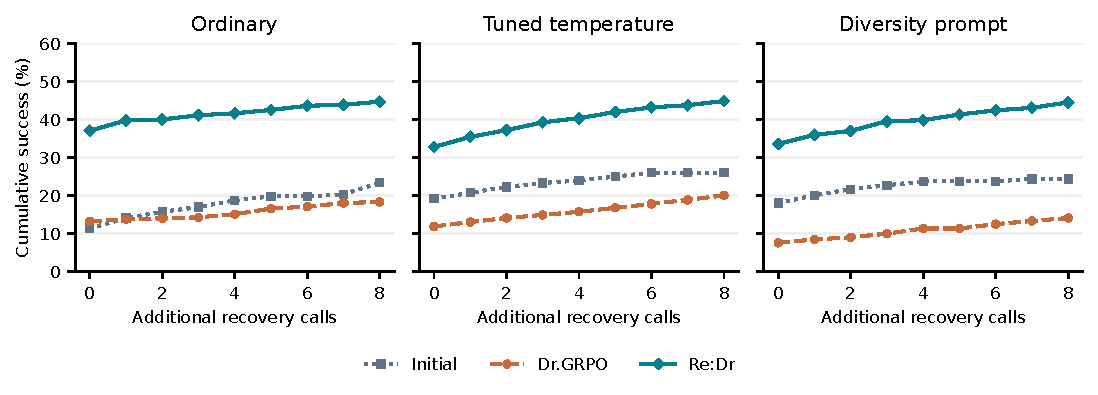
\includegraphics[width=\linewidth]{figures/pantry_adaptation_recovery_20260912.pdf}
\caption{\textbf{Re:Dr improves portfolio survival and success within eight
recovery calls.} Panels compare ordinary sampling, tuned temperature, and
diversity prompting on the same 181 feasible ingredient outages from 32
\texttt{PantryPlan} problems. The horizontal axis is the additional recovery-call budget;
the vertical axis includes success without recovery at zero calls. Curves
average outages within problems, then problems equally. Solid diamonds show
Re:Dr, dashed circles Dr.GRPO, and dotted squares the initial checkpoint;
trained curves average two matched seeds. Pointwise 95\% intervals for
paired differences appear in Table~\ref{tab:pantry-adaptation-contrasts}.}
\label{fig:pantry-adaptation-recovery}
\end{figure}

\begin{table}[!htbp]
\centering
\caption{\textbf{Re:Dr portfolios adapt better to ingredient outages across all three sampling strategies.} Eight initial plans face 181 feasible outages from 32 problems or five additional dietary restrictions from five problems. Survival is success without recovery; By 8 includes success within eight recovery calls (both percentages). Calls count unresolved cases as eight. Token totals count the initial portfolio once per revised task. Entries average perturbations within problems, then problems equally; dietary estimates use only five problems. Labels (a) and (b) denote the two matched training replicates.}
\label{tab:pantry-adaptation}
\scriptsize
\setlength{\tabcolsep}{3pt}
\begin{tabular}{lllrrrrr}
\toprule
Change & Checkpoint & Strategy & Survival & By 8 & Calls & Input tokens & Output tokens \\
\midrule
Outages & Initial & Ordinary & 11.35 & 23.44 & 6.63 & 11301.75 & 376.49 \\
 & Initial & Tuned temperature & 19.17 & 26.04 & 6.13 & 10864.88 & 370.17 \\
 & Initial & Diversity prompt & 18.02 & 24.38 & 6.22 & 11794.81 & 352.87 \\
 & Dr.GRPO (a) & Ordinary & 9.79 & 14.01 & 7.09 & 12439.22 & 823.70 \\
 & Dr.GRPO (a) & Tuned temperature & 13.44 & 16.77 & 6.79 & 12017.57 & 775.44 \\
 & Dr.GRPO (a) & Diversity prompt & 5.21 & 8.39 & 7.44 & 14103.23 & 848.09 \\
 & Dr.GRPO (b) & Ordinary & 16.67 & 22.60 & 6.47 & 11265.39 & 637.59 \\
 & Dr.GRPO (b) & Tuned temperature & 10.31 & 23.39 & 6.75 & 11531.40 & 644.94 \\
 & Dr.GRPO (b) & Diversity prompt & 9.90 & 19.79 & 6.90 & 13124.10 & 731.00 \\
 & Re:Dr (a) & Ordinary & 39.38 & 47.97 & 4.47 & 9078.92 & 297.98 \\
 & Re:Dr (a) & Tuned temperature & 28.23 & 40.94 & 5.19 & 9718.01 & 310.50 \\
 & Re:Dr (a) & Diversity prompt & 36.93 & 47.19 & 4.68 & 10465.22 & 344.02 \\
 & Re:Dr (b) & Ordinary & 34.74 & 41.51 & 4.94 & 9547.16 & 308.52 \\
 & Re:Dr (b) & Tuned temperature & 37.34 & 48.85 & 4.53 & 9148.77 & 300.05 \\
 & Re:Dr (b) & Diversity prompt & 30.26 & 41.93 & 5.06 & 10584.02 & 313.50 \\
\midrule
Dietary & Initial & Ordinary & 0.00 & 20.00 & 6.80 & 11392.80 & 371.20 \\
 & Initial & Tuned temperature & 20.00 & 40.00 & 6.40 & 11175.20 & 387.20 \\
 & Initial & Diversity prompt & 0.00 & 0.00 & 8.00 & 13630.20 & 405.00 \\
 & Dr.GRPO (a) & Ordinary & 0.00 & 0.00 & 8.00 & 13310.20 & 849.20 \\
 & Dr.GRPO (a) & Tuned temperature & 0.00 & 0.00 & 8.00 & 13394.60 & 856.00 \\
 & Dr.GRPO (a) & Diversity prompt & 0.00 & 0.00 & 8.00 & 15045.40 & 939.60 \\
 & Dr.GRPO (b) & Ordinary & 0.00 & 20.00 & 7.40 & 12063.00 & 650.40 \\
 & Dr.GRPO (b) & Tuned temperature & 0.00 & 0.00 & 8.00 & 12544.20 & 615.40 \\
 & Dr.GRPO (b) & Diversity prompt & 0.00 & 0.00 & 8.00 & 14132.40 & 725.60 \\
 & Re:Dr (a) & Ordinary & 20.00 & 60.00 & 5.20 & 9732.60 & 326.00 \\
 & Re:Dr (a) & Tuned temperature & 40.00 & 40.00 & 4.80 & 9402.80 & 307.60 \\
 & Re:Dr (a) & Diversity prompt & 40.00 & 40.00 & 4.80 & 10693.60 & 355.60 \\
 & Re:Dr (b) & Ordinary & 40.00 & 80.00 & 3.20 & 7853.20 & 271.20 \\
 & Re:Dr (b) & Tuned temperature & 40.00 & 80.00 & 3.60 & 8127.80 & 265.20 \\
 & Re:Dr (b) & Diversity prompt & 20.00 & 40.00 & 5.00 & 10738.20 & 341.00 \\
\bottomrule
\end{tabular}
\end{table}


\begin{table}[!htbp]
\centering
\caption{\textbf{Re:Dr raises outage survival and reduces recovery calls.} Entries are Re:Dr minus Dr.GRPO, averaged over two matched seeds on 32 paired problems. Survival and success by eight calls are percentage-point differences; calls include unresolved cases. Brackets are pointwise 95\% paired problem-bootstrap intervals, conditional on the observed training seeds.}
\label{tab:pantry-adaptation-contrasts}
\scriptsize
\setlength{\tabcolsep}{3pt}
\begin{tabular}{lrrr}
\toprule
Strategy & $\Delta$ survival & $\Delta$ by 8 calls & $\Delta$ calls \\
\midrule
Ordinary & $23.83$ $[12.16, 35.89]$ & $26.43$ $[14.69, 38.18]$ & $-2.08$ $[-3.03, -1.14]$ \\
Tuned temperature & $20.91$ $[9.19, 32.89]$ & $24.82$ $[14.04, 35.52]$ & $-1.91$ $[-2.78, -1.05]$ \\
Diversity prompt & $26.04$ $[16.93, 35.65]$ & $30.47$ $[21.51, 39.27]$ & $-2.30$ $[-3.04, -1.57]$ \\
\bottomrule
\end{tabular}
\end{table}

With ordinary sampling, Re:Dr improves survival over Dr.GRPO by 23.83 percentage points
$[12.16,35.89]$, reduces the mean number of recovery calls, capped at eight, by 2.08
$[1.14,3.03]$, and improves success within eight recovery calls by 26.43 points
$[14.69,38.18]$. Mean input and output token totals fall by 2,539.27
$[1,618.01,3,468.86]$ and 427.40 $[386.83,466.30]$, respectively.
The initial portfolios also contain 1.234 more correct responses out of
eight $[.578,1.984]$. Restricting each paired-seed comparison to portfolios
with equal observed correct counts leaves a 1.05-percentage-point survival
gain $[0.00,3.53]$. We first average eligible seed comparisons within each
problem, then average the 19 problems with at least one eligible comparison.
This restriction changes both the problem and seed composition, and equal
observed counts do not establish equal underlying accuracy. The adaptation
gains therefore do not isolate diversity as their causal mechanism.

Per-perturbation token totals represent deploying one portfolio and recovering
from one change in requirements. Input counts include reused prefixes and
do not measure the compute saved by prefix caching. Table~\ref{tab:pantry-collection-cost}
counts each response once across temperature selection, initial portfolios
from tuned-temperature sampling and diversity prompting, and recovery under
all three strategies. It excludes ordinary initial-portfolio generation.
Neither inference cost summary includes training costs.

\begin{table}[!htbp]
\centering
\caption{\textbf{Inference costs include temperature selection and recovery.} Each checkpoint selects $T$ from 384 responses on 16 development problems. Inference totals include this calibration, initial portfolios for tuned-temperature and diversity prompting, and recovery under all three strategies on 32 evaluation problems. Ordinary initial-portfolio generation is excluded. Each response is counted once, including reused input prefixes. Seconds report generation time, excluding training, without hardware normalization. Labels (a) and (b) denote matched training replicates.}
\label{tab:pantry-collection-cost}
\scriptsize
\setlength{\tabcolsep}{3pt}
\begin{tabular}{llrrrrr}
\toprule
Checkpoint & Scope & $T$ & Responses & Input tokens & Output tokens & Seconds \\
\midrule
Dr.GRPO (a) & Calibration & 1.3 & 384 & 229392 & 19871 & 136.3 \\
Dr.GRPO (a) & Inference total & 1.3 & 4874 & 4870884 & 272484 & 3302.0 \\
Dr.GRPO (b) & Calibration & 1.3 & 384 & 229392 & 15544 & 126.5 \\
Dr.GRPO (b) & Inference total & 1.3 & 4634 & 4365524 & 220458 & 2792.9 \\
Re:Dr (a) & Calibration & 0.7 & 384 & 229392 & 8552 & 111.1 \\
Re:Dr (a) & Inference total & 0.7 & 3559 & 3160284 & 92227 & 1527.7 \\
Re:Dr (b) & Calibration & 1.0 & 384 & 229392 & 8585 & 112.5 \\
Re:Dr (b) & Inference total & 1.0 & 3592 & 3169337 & 88300 & 1510.2 \\
Initial & Calibration & 1.3 & 384 & 229392 & 9521 & 123.5 \\
Initial & Inference total & 1.3 & 4416 & 4035069 & 116619 & 1957.4 \\
\bottomrule
\end{tabular}
\end{table}


\subsection{Complementarity across hosted models}
\label{app:cross-model-overlap}
Seven hosted models each produce eight responses to the same 1,920 prompts
(five domains, three levels, and 128 prompts per domain and level), totaling
107,520 responses. We use strict grading and the original Opus 5 \texttt{Python}
interface; the formatting-normalized hosted comparison uses a revised
Opus 5 interface. For each of the 21 model pairs, a mixed portfolio draws four
responses without replacement from each model's eight-response pool. We
compute its expected distinct-mode count exactly over all $\binom{8}{4}^2=4{,}900$
subset pairs, then compare with each constituent's complete eight-response
portfolio and their average. These are expectations within the finite
response pools, conditional on the outputs generated.

Every mixture increases the expected number of distinct solution modes
relative to its average constituent by $.115$--$.266$. Ten pairs improve
on both constituents in point estimates; nine have pointwise intervals
entirely above zero against both. On
prompts with at least four correct responses from each model, we also compare
a mixture of two correct draws per model with four correct draws from either
constituent. All pairwise gains over the average constituent remain positive
($.073$--$.177$ modes). Fixing the number of correct draws conditions on a
different eligible subset for each pair. It does not equate accuracy or the
number of attempts required to obtain those correct responses.

\begin{table}[!htbp]
\centering
\caption{\textbf{Every model pair increases expected distinct modes over its average constituent.} A 4+4 mixture samples without replacement from the two eight-response pools; A and B name the constituents in order. Panel A compares with their average: fine and coarse keys use all 1,920 prompts, while the four-correct-draw comparison uses $n$ prompts with at least four correct responses per model (2+2 mixed versus four per constituent). Panel B compares fine-key distinct modes with each constituent and pass@8 with their average. Entries are distinct-mode differences except pass@8, in percentage points. Brackets are pointwise 95\% paired problem-bootstrap intervals, stratified by domain and level; comparisons share models and prompts.}
\label{tab:cross-model-mixtures}
\scriptsize
\setlength{\tabcolsep}{3pt}
\textbf{A}\par\smallskip
\resizebox{\linewidth}{!}{%
\begin{tabular}{lrrrr}
\toprule
Pair & Fine & Coarse & Four correct draws & $n$ \\
\midrule
DeepSeek V4 Pro + Kimi K3 & $0.148$ $[0.136, 0.160]$ & $0.142$ $[0.131, 0.154]$ & $0.107$ $[0.098, 0.115]$ & 1858 \\
DeepSeek V4 Pro + Opus 4.8 & $0.198$ $[0.185, 0.211]$ & $0.183$ $[0.171, 0.197]$ & $0.153$ $[0.142, 0.164]$ & 1847 \\
DeepSeek V4 Pro + Opus 5 & $0.262$ $[0.249, 0.275]$ & $0.252$ $[0.240, 0.265]$ & $0.177$ $[0.165, 0.190]$ & 1510 \\
DeepSeek V4 Pro + GPT-5.4 & $0.133$ $[0.122, 0.143]$ & $0.127$ $[0.116, 0.138]$ & $0.098$ $[0.090, 0.107]$ & 1695 \\
DeepSeek V4 Pro + GPT-5.6 Sol & $0.235$ $[0.223, 0.247]$ & $0.224$ $[0.212, 0.237]$ & $0.154$ $[0.142, 0.166]$ & 1396 \\
DeepSeek V4 Pro + Grok 4.3 & $0.123$ $[0.112, 0.134]$ & $0.117$ $[0.106, 0.127]$ & $0.091$ $[0.083, 0.099]$ & 1859 \\
Kimi K3 + Opus 4.8 & $0.187$ $[0.174, 0.200]$ & $0.172$ $[0.159, 0.185]$ & $0.138$ $[0.127, 0.148]$ & 1885 \\
Kimi K3 + Opus 5 & $0.266$ $[0.253, 0.279]$ & $0.255$ $[0.242, 0.268]$ & $0.162$ $[0.150, 0.175]$ & 1543 \\
Kimi K3 + GPT-5.4 & $0.127$ $[0.115, 0.139]$ & $0.112$ $[0.101, 0.124]$ & $0.083$ $[0.075, 0.092]$ & 1720 \\
Kimi K3 + GPT-5.6 Sol & $0.202$ $[0.190, 0.214]$ & $0.195$ $[0.183, 0.207]$ & $0.093$ $[0.083, 0.104]$ & 1417 \\
Kimi K3 + Grok 4.3 & $0.115$ $[0.104, 0.126]$ & $0.110$ $[0.099, 0.121]$ & $0.073$ $[0.066, 0.080]$ & 1900 \\
Opus 4.8 + Opus 5 & $0.187$ $[0.176, 0.199]$ & $0.182$ $[0.171, 0.193]$ & $0.098$ $[0.087, 0.109]$ & 1534 \\
Opus 4.8 + GPT-5.4 & $0.201$ $[0.186, 0.215]$ & $0.185$ $[0.172, 0.199]$ & $0.156$ $[0.144, 0.168]$ & 1713 \\
Opus 4.8 + GPT-5.6 Sol & $0.247$ $[0.234, 0.261]$ & $0.237$ $[0.223, 0.250]$ & $0.151$ $[0.138, 0.164]$ & 1409 \\
Opus 4.8 + Grok 4.3 & $0.180$ $[0.167, 0.194]$ & $0.171$ $[0.158, 0.184]$ & $0.141$ $[0.130, 0.153]$ & 1894 \\
Opus 5 + GPT-5.4 & $0.228$ $[0.215, 0.241]$ & $0.217$ $[0.204, 0.230]$ & $0.158$ $[0.145, 0.171]$ & 1493 \\
Opus 5 + GPT-5.6 Sol & $0.169$ $[0.157, 0.182]$ & $0.161$ $[0.149, 0.174]$ & $0.143$ $[0.130, 0.156]$ & 1370 \\
Opus 5 + Grok 4.3 & $0.231$ $[0.219, 0.244]$ & $0.225$ $[0.213, 0.237]$ & $0.145$ $[0.133, 0.157]$ & 1547 \\
GPT-5.4 + GPT-5.6 Sol & $0.156$ $[0.145, 0.167]$ & $0.147$ $[0.136, 0.158]$ & $0.094$ $[0.084, 0.104]$ & 1400 \\
GPT-5.4 + Grok 4.3 & $0.130$ $[0.119, 0.142]$ & $0.121$ $[0.111, 0.132]$ & $0.095$ $[0.086, 0.104]$ & 1722 \\
GPT-5.6 Sol + Grok 4.3 & $0.211$ $[0.199, 0.224]$ & $0.204$ $[0.192, 0.216]$ & $0.118$ $[0.107, 0.130]$ & 1418 \\
\bottomrule
\end{tabular}
}
\par\medskip
\textbf{B}\par\smallskip
\resizebox{\linewidth}{!}{%
\begin{tabular}{lrrr}
\toprule
Pair & $\Delta D$ vs A & $\Delta D$ vs B & $\Delta$ pass@8 vs mean \\
\midrule
DeepSeek V4 Pro + Kimi K3 & $0.279$ $[0.254, 0.304]$ & $0.017$ $[-0.008, 0.043]$ & $0.22$ $[0.08, 0.39]$ \\
DeepSeek V4 Pro + Opus 4.8 & $0.089$ $[0.064, 0.114]$ & $0.307$ $[0.282, 0.332]$ & $0.31$ $[0.15, 0.49]$ \\
DeepSeek V4 Pro + Opus 5 & $-0.061$ $[-0.082, -0.039]$ & $0.585$ $[0.560, 0.610]$ & $7.48$ $[7.19, 7.78]$ \\
DeepSeek V4 Pro + GPT-5.4 & $0.097$ $[0.074, 0.121]$ & $0.168$ $[0.145, 0.192]$ & $0.64$ $[0.41, 0.90]$ \\
DeepSeek V4 Pro + GPT-5.6 Sol & $-0.003$ $[-0.025, 0.019]$ & $0.473$ $[0.447, 0.500]$ & $7.16$ $[6.71, 7.62]$ \\
DeepSeek V4 Pro + Grok 4.3 & $0.059$ $[0.037, 0.082]$ & $0.186$ $[0.163, 0.210]$ & $0.34$ $[0.17, 0.52]$ \\
Kimi K3 + Opus 4.8 & $-0.053$ $[-0.080, -0.027]$ & $0.427$ $[0.401, 0.452]$ & $0.19$ $[0.07, 0.32]$ \\
Kimi K3 + Opus 5 & $-0.188$ $[-0.212, -0.165]$ & $0.719$ $[0.692, 0.747]$ & $7.34$ $[7.08, 7.61]$ \\
Kimi K3 + GPT-5.4 & $-0.040$ $[-0.064, -0.015]$ & $0.293$ $[0.267, 0.320]$ & $0.73$ $[0.48, 1.00]$ \\
Kimi K3 + GPT-5.6 Sol & $-0.167$ $[-0.191, -0.144]$ & $0.571$ $[0.543, 0.600]$ & $7.38$ $[6.92, 7.85]$ \\
Kimi K3 + Grok 4.3 & $-0.080$ $[-0.104, -0.056]$ & $0.309$ $[0.284, 0.335]$ & $0.12$ $[0.03, 0.23]$ \\
Opus 4.8 + Opus 5 & $-0.027$ $[-0.045, -0.009]$ & $0.401$ $[0.379, 0.423]$ & $7.42$ $[7.14, 7.71]$ \\
Opus 4.8 + GPT-5.4 & $0.274$ $[0.248, 0.300]$ & $0.127$ $[0.101, 0.153]$ & $0.93$ $[0.65, 1.24]$ \\
Opus 4.8 + GPT-5.6 Sol & $0.118$ $[0.096, 0.141]$ & $0.377$ $[0.350, 0.403]$ & $7.51$ $[7.03, 7.99]$ \\
Opus 4.8 + Grok 4.3 & $0.226$ $[0.202, 0.250]$ & $0.135$ $[0.110, 0.160]$ & $0.11$ $[0.02, 0.23]$ \\
Opus 5 + GPT-5.4 & $0.515$ $[0.489, 0.541]$ & $-0.060$ $[-0.082, -0.037]$ & $6.30$ $[5.90, 6.71]$ \\
Opus 5 + GPT-5.6 Sol & $0.254$ $[0.232, 0.277]$ & $0.084$ $[0.063, 0.106]$ & $2.11$ $[1.66, 2.57]$ \\
Opus 5 + Grok 4.3 & $0.490$ $[0.467, 0.514]$ & $-0.028$ $[-0.048, -0.007]$ & $7.41$ $[7.13, 7.69]$ \\
GPT-5.4 + GPT-5.6 Sol & $-0.046$ $[-0.067, -0.025]$ & $0.359$ $[0.335, 0.383]$ & $5.61$ $[5.15, 6.08]$ \\
GPT-5.4 + Grok 4.3 & $0.102$ $[0.078, 0.127]$ & $0.159$ $[0.135, 0.182]$ & $0.93$ $[0.65, 1.23]$ \\
GPT-5.6 Sol + Grok 4.3 & $0.386$ $[0.360, 0.412]$ & $0.037$ $[0.015, 0.058]$ & $7.55$ $[7.08, 8.04]$ \\
\bottomrule
\end{tabular}
}
\end{table}

Cross-model collision ranges from $.624$ to $.740$, compared with $.704$
to $.819$ for mean within-model collision. Each pair gives equal weight
to prompts with $\geq2$ correct responses from each model. Absence of
observed overlap does not establish disjoint supports. Gains relative to
the average constituent persist with coarser keys and formatting-normalized
grading. Equal response counts do not equate token use, compute, monetary
cost, or reasoning interfaces across providers. These comparisons of finite
response pools do not identify causal training mechanisms.

\subsection{Sensitivity to task-relevant equivalences}
\label{app:coarser-keys}
We merge solution keys according to task-relevant equivalences and recompute
diversity. \texttt{Graph} merges global color renamings that fix every anchored color;
vertex identities remain fixed. \texttt{Python} groups opposite members $d$ and $n/d$ of the
same unordered proper factor pair, retaining input-vector order. \texttt{Countdown}
flattens associative additions and multiplications and sorts their children,
preserving operands, multiplicity, and subtraction/division boundaries.
\texttt{MathIR} retains its simplified state trajectory, and \texttt{PantryPlan} retains
ingredient supports, whose differences can affect survival under outages. The same domain-specific
map applies to each model's correct responses. Correctness is unchanged;
deterministic merging cannot increase the observed distinct-mode count or
reduce correct-pair collision.

Uniform mass over fine keys generally induces unequal mass across coarse
groups. For \texttt{Graph} and \texttt{Python}, exhaustive enumeration determines both the
number of coarse groups and their sizes, allowing separate collision
references for uniform fine-key mass and uniform coarse-group mass.
\texttt{Countdown}'s full verifier support is unknown, so these uniform references
cannot be computed for that domain.

\begin{table}[!htbp]
\centering
\caption{\textbf{Coarser keys reduce observed mode counts and increase collision.} Strict grading uses eight responses per hosted model on 1,920 prompts. $D@8$ averages all prompts; collision averages prompts with at least two correct responses, with eligibility varying by model. Brackets are pointwise 95\% paired problem-bootstrap intervals, stratified by domain and level.}
\label{tab:hosted-coarse-keys}
\scriptsize
\setlength{\tabcolsep}{3pt}
\begin{tabular}{lrrrr}
\toprule
Model & Fine D@8 & Coarse D@8 & Fine collision & Coarse collision \\
\midrule
DeepSeek V4 Pro & $1.826$ $[1.792, 1.859]$ & $1.762$ $[1.729, 1.795]$ & $0.720$ $[0.710, 0.731]$ & $0.739$ $[0.729, 0.750]$ \\
Kimi K3 & $2.087$ $[2.047, 2.129]$ & $1.952$ $[1.913, 1.992]$ & $0.688$ $[0.678, 0.699]$ & $0.723$ $[0.712, 0.733]$ \\
Opus 4.8 & $1.608$ $[1.575, 1.641]$ & $1.556$ $[1.525, 1.588]$ & $0.795$ $[0.785, 0.805]$ & $0.811$ $[0.801, 0.821]$ \\
Opus 5 & $1.180$ $[1.155, 1.206]$ & $1.152$ $[1.128, 1.177]$ & $0.856$ $[0.845, 0.866]$ & $0.867$ $[0.857, 0.877]$ \\
GPT-5.4 & $1.755$ $[1.718, 1.792]$ & $1.679$ $[1.644, 1.715]$ & $0.729$ $[0.717, 0.741]$ & $0.750$ $[0.739, 0.762]$ \\
GPT-5.6 Sol & $1.349$ $[1.317, 1.382]$ & $1.312$ $[1.281, 1.345]$ & $0.778$ $[0.765, 0.790]$ & $0.794$ $[0.782, 0.806]$ \\
Grok 4.3 & $1.698$ $[1.665, 1.732]$ & $1.645$ $[1.613, 1.679]$ & $0.791$ $[0.782, 0.800]$ & $0.807$ $[0.798, 0.816]$ \\
\bottomrule
\end{tabular}
\end{table}


\begin{table}[!htbp]
\centering
\caption{\textbf{\texttt{Python} diversity gains depend on the factor-pair equivalence and prompt wording.} Entries give Re:Dr minus Dr.GRPO in distinct modes from eight strictly graded responses. Level-2 trained Qwen2.5-0.5B checkpoints use 32 paired evaluation problems per level; means weight seeds equally. Brackets are pointwise 95\% paired problem-bootstrap intervals, conditional on those checkpoints. Fine and coarse keys coincide for \texttt{MathIR} and \texttt{PantryPlan}.}
\label{tab:local-coarse-keys}
\scriptsize
\setlength{\tabcolsep}{3pt}
\begin{tabular}{lrllrr}
\toprule
Domain & Level & Wording & Seeds & Fine $\Delta D@8$ & Coarse $\Delta D@8$ \\
\midrule
\texttt{Python} & 2 & original & 5 & $0.431$ $[0.406, 0.456]$ & $0.075$ $[0.025, 0.138]$ \\
\texttt{MathIR} & 2 & original & 5 & $0.463$ $[0.387, 0.531]$ & $0.463$ $[0.387, 0.531]$ \\
\texttt{PantryPlan} & 2 & original & 2 & $0.469$ $[0.203, 0.750]$ & $0.469$ $[0.203, 0.750]$ \\
\texttt{Python} & 3 & original & 5 & $0.419$ $[0.400, 0.444]$ & $0.000$ $[0.000, 0.000]$ \\
\texttt{MathIR} & 3 & original & 5 & $0.119$ $[0.019, 0.225]$ & $0.119$ $[0.019, 0.225]$ \\
\texttt{PantryPlan} & 3 & original & 2 & $0.125$ $[-0.109, 0.375]$ & $0.125$ $[-0.109, 0.375]$ \\
\texttt{Python} & 2 & neutral & 5 & $0.675$ $[0.519, 0.838]$ & $0.556$ $[0.438, 0.675]$ \\
\texttt{MathIR} & 2 & neutral & 5 & $0.469$ $[0.375, 0.562]$ & $0.469$ $[0.375, 0.562]$ \\
\texttt{PantryPlan} & 2 & neutral & 2 & $0.484$ $[0.234, 0.766]$ & $0.484$ $[0.234, 0.766]$ \\
\texttt{Python} & 3 & neutral & 5 & $0.656$ $[0.537, 0.775]$ & $0.500$ $[0.419, 0.575]$ \\
\texttt{MathIR} & 3 & neutral & 5 & $0.119$ $[0.025, 0.213]$ & $0.119$ $[0.025, 0.213]$ \\
\texttt{PantryPlan} & 3 & neutral & 2 & $0.250$ $[-0.031, 0.562]$ & $0.250$ $[-0.031, 0.562]$ \\
\bottomrule
\end{tabular}
\end{table}

With coarser \texttt{Python} keys, the Re:Dr-minus-Dr.GRPO gain in distinct modes
under original wording falls from $.419$ to zero at Level~3 and from
$.431$ to $.075$ at Level~2. Under neutral wording, the gains remain
$.556$ at Level~2 and $.500$ at Level~3. The original-wording effect can
therefore reflect opposite members of the same factor pair. Its interpretation
depends on both prompt wording and the definition of a solution mode;
neither divisor vectors nor factor-pair vectors identify different algorithms.


% Generated by ops/build_paper_portfolio_withdrawals.py; do not edit numbers.
\section{Portfolio Survival under Withdrawn Options}
\label{app:portfolio-withdrawals}
A portfolio survives a withdrawn option if at least one of its solutions
remains valid. We evaluate survival across all five domains in 474 terminal checkpoint evaluations, each
with 128 prompts and four groups of eight responses per prompt. The groups have
overlapping sampling streams (App.~\ref{app:conditional-concentration}). Replay's
largest gains in expected distinct modes at four verified draws occur in
\texttt{Graph}, \texttt{Countdown}, \texttt{Python} and \texttt{PantryPlan}. Across 38 matched
domain--scale--level--objective comparisons,
\pmd{} gains correlate with survival gains at four verified draws
(Pearson $r=.57$).

\paragraph{Task perturbations.} Each task loses one option: a colour at one
vertex (\texttt{Graph}), an arithmetic operation (\texttt{Countdown}), a returned divisor value
(\texttt{Python}), a menu action (\texttt{MathIR}), or an ingredient (\texttt{PantryPlan}; see
App.~\ref{app:pantry-adaptation}). Options are enumerated from the task
specification. The solution-mode enumeration matches the certified counts for
all 1{,}280 prompts. A surviving certified mode establishes feasibility.
When the certified count is only a lower bound on the verifier's full support,
absence of a surviving mode from the enumeration does not establish infeasibility. Of
9{,}864 options, 9{,}118 retain at least one certified mode. Among these,
8{,}308 are binding: they also remove at least one certified mode. We evaluate
both the binding set and the full set with a feasibility certificate.

\paragraph{Survival criterion.} Each portfolio contains the verified
responses among eight draws. It survives when at least one of these solutions
remains valid after the option is removed. \texttt{Graph}, \texttt{Countdown} and \texttt{Python} determine this directly from
the outcome key, including verified keys outside the enumeration. \texttt{Countdown}
contributes 2 such keys, observed 50 times among the
846{,}398 verified draws in this evaluation: the verifier accepts unary negation, which the
expression enumeration omits. For \texttt{MathIR}, re-enumerating the reduced menu tests
whether the same executed state path remains realizable, possibly through a
different action sequence. For \texttt{PantryPlan}, we test the certified plan
associated with each ingredient-support key. All observed \texttt{MathIR} and \texttt{PantryPlan} keys belong to their
respective enumerations.

\paragraph{Survival conditional on correct draws.} Raw survival depends on
both correctness and the distribution of valid modes. At budgets $m=1,2,4$, we
compute the exact expected survival of a uniformly selected $m$-element subset
of a portfolio's verified draws, as in App.~\ref{app:cross-model-overlap}.
Replay--control contrasts use only prompt--group pairs with at least $m$
verified draws under both methods, so eligibility can change with $m$.
Fixing the number of correct draws does not equalize policy accuracy.
A survival difference can also arise because the modes one method favors are
individually more robust to withdrawals, so a gain that grows with $m$ does
not by itself isolate the contribution of diversity. Expected distinct modes
at the same budget therefore serve as a separate measure of portfolio breadth.

\begin{table}[!htbp]
\centering
\caption{\textbf{Binding withdrawals remove certified modes while retaining a feasibility certificate.} Each row covers 128 prompts. Support is the mean certified mode count per prompt; Options counts single withdrawals. Binding counts options that retain at least one certified mode and remove at least one. Kept is the mean retained fraction of certified modes across binding options. Pairs counts binding pairs of withdrawals, and Kept$_2$ gives the corresponding retained fraction.}
\label{tab:withdrawal-inventory}
\scriptsize
\setlength{\tabcolsep}{3pt}
\begin{tabular}{llrrrrrrr}
\toprule
Domain & Level & Prompts & Support & Options & Binding & Kept & Pairs & Kept$_2$ \\
\midrule
\texttt{Graph} & 1 & 128 & 6.3 & 1152 & 818 & 0.57 & 1957 & 0.34 \\
\texttt{Graph} & 2 & 128 & 6.1 & 1536 & 1068 & 0.57 & 3457 & 0.35 \\
\texttt{Countdown} & 1 & 128 & 4.5 & 512 & 147 & 0.48 & 21 & 0.44 \\
\texttt{Countdown} & 2 & 128 & 4.4 & 512 & 185 & 0.49 & 40 & 0.37 \\
\texttt{Python} & 1 & 128 & 229.4 & 1433 & 1433 & 0.68 & 7716 & 0.50 \\
\texttt{Python} & 2 & 128 & 251.7 & 1647 & 1647 & 0.71 & 10381 & 0.55 \\
\texttt{MathIR} & 1 & 128 & 5.0 & 768 & 448 & 0.40 & 384 & 0.23 \\
\texttt{MathIR} & 2 & 128 & 5.0 & 768 & 512 & 0.45 & 512 & 0.25 \\
\texttt{PantryPlan} & 1 & 128 & 18.2 & 768 & 651 & 0.44 & 1231 & 0.18 \\
\texttt{PantryPlan} & 2 & 128 & 18.2 & 768 & 653 & 0.45 & 1228 & 0.19 \\
\bottomrule
\end{tabular}
\end{table}
\begin{table}[!htbp]
\centering
\caption{\textbf{Both replay arms improve four-draw survival in \texttt{Graph}, \texttt{Python} and \texttt{PantryPlan}.} Each replay arm is compared with its fresh-objective control. Survival differences are percentage points; $\Delta D_4$ is the difference in expected distinct modes at four verified draws. Raw uses all eight responses; Budget columns use the indicated number of verified draws. Fixed-correct-draw results pool jointly eligible prompt--group pairs across matched seeds, scales and levels; raw results use all paired groups. All columns use binding options except Budget 4 (all), which includes every option with a feasibility certificate. Brackets are pointwise 95\% intervals from 20{,}000 paired bootstrap replicates. Each resampled cluster is a prompt within one level and scale, with its groups and seeds kept together; copies at other scales are separate clusters. Intervals condition on the observed seeds.}
\label{tab:withdrawal-contrasts}
\scriptsize
\setlength{\tabcolsep}{3pt}
\begin{tabular}{llrrrrrr}
\toprule
Domain & Arm & Raw & Budget 1 & Budget 2 & Budget 4 & Budget 4 (all) & $\Delta D_4$ \\
\midrule
\texttt{Graph} & Re:Dr & $34.78$ & $0.00$ $[0.00, 0.00]$ & $10.51$ $[8.76, 12.31]$ & $19.65$ $[15.61, 23.82]$ & $15.66$ & 1.290 \\
\texttt{Graph} & Re:Max & $18.98$ & $0.00$ $[0.00, 0.00]$ & $6.62$ $[5.23, 7.98]$ & $10.99$ $[8.25, 13.81]$ & $8.31$ & 0.646 \\
\texttt{Countdown} & Re:Dr & $5.32$ & $3.51$ $[1.88, 5.30]$ & $6.52$ $[4.27, 8.94]$ & $9.58$ $[6.81, 12.63]$ & $2.53$ & 0.626 \\
\texttt{Countdown} & Re:Max & $1.95$ & $-2.40$ $[-4.62, -0.21]$ & $-1.25$ $[-3.70, 1.14]$ & $0.10$ $[-2.62, 2.78]$ & $-0.05$ & 0.490 \\
\texttt{Python} & Re:Dr & $38.99$ & $-0.22$ $[-1.25, 0.91]$ & $4.09$ $[3.17, 5.08]$ & $7.67$ $[6.82, 8.58]$ & $7.67$ & 0.317 \\
\texttt{Python} & Re:Max & $22.84$ & $1.53$ $[0.87, 2.24]$ & $3.85$ $[3.04, 4.72]$ & $5.68$ $[4.80, 6.64]$ & $5.68$ & 0.198 \\
\texttt{MathIR} & Re:Dr & $33.61$ & $0.01$ $[0.00, 0.05]$ & $0.12$ $[0.03, 0.23]$ & $0.14$ $[0.00, 0.30]$ & $0.08$ & 0.004 \\
\texttt{MathIR} & Re:Max & $21.64$ & $0.00$ $[-0.04, 0.05]$ & $0.03$ $[-0.03, 0.10]$ & $0.09$ $[-0.01, 0.21]$ & $0.06$ & 0.003 \\
\texttt{PantryPlan} & Re:Dr & $16.55$ & $-1.11$ $[-1.65, -0.54]$ & $4.36$ $[3.82, 4.87]$ & $9.78$ $[8.90, 10.65]$ & $9.20$ & 0.810 \\
\texttt{PantryPlan} & Re:Max & $13.04$ & $-0.64$ $[-1.04, -0.21]$ & $3.12$ $[2.72, 3.53]$ & $6.61$ $[5.83, 7.39]$ & $6.20$ & 0.547 \\
\bottomrule
\end{tabular}
\end{table}
Raw survival improves in 39 of 40 domain--scale--level--objective
comparisons. At four verified draws, the point estimate is positive in
28 of 39 eligible comparisons; these conditional comparisons cover
fewer prompt--group pairs than raw survival. Outside \texttt{MathIR}, Re:Dr adds between
$.3$ and $1.3$ expected distinct modes at four verified draws, and its pooled
survival gains reach 19.6 percentage points. In \texttt{MathIR}, the corresponding
gains are only $.004$ distinct modes and $.14$ survival points, with an interval
of $[.00,.30]$ after rounding. These small positive estimates are consistent
with the small \pmd{} gain in Table~\ref{tab:cross-scale-terminal-effects}.

\texttt{Graph}'s one-draw contrast is zero by construction. Each binding withdrawal
removes one color at one vertex, and each valid coloring is excluded by
exactly one such withdrawal per variable vertex, so every individual mode
survives the same fraction of binding withdrawals. Including nonbinding options shrinks the contrasts,
because those options leave every certified mode intact; for example,
63\% of \texttt{Countdown} Level-1 options with a feasibility certificate are nonbinding.
The Budget 4 (all) and binding columns therefore describe different withdrawal
populations.
\begin{figure}[!htbp]
  \centering
  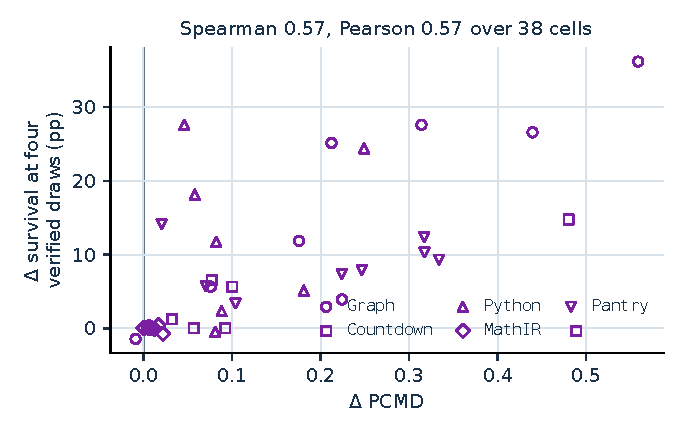
\includegraphics[width=0.62\linewidth]{figures/withdrawal_pmd_agreement.pdf}
  \caption{\textbf{Diversity gains correlate with survival gains after a withdrawal.} Each mark is one replay--fresh-objective contrast in a domain, scale and level. The horizontal axis is the terminal \pmd{} difference; the vertical axis is the percentage-point survival difference at four verified draws, averaged equally over eligible seed-specific contrasts. Survival uses jointly eligible prompt--group pairs within each seed. Marker shape identifies the domain; zero lines mark no change. The 38 comparisons have Pearson and Spearman correlations of $.57$; points show estimates without intervals. The association is descriptive, and the two metrics need not use the same eligible population.}
  \label{fig:withdrawal-pmd-agreement}
\end{figure}

\subsection{Two withdrawals at once}
\label{app:withdrawal-severity}
We next remove two binding options at once. Of the 29{,}213 pairs of binding
single withdrawals, 26{,}927 retain at least one certified mode and enter the
survival comparison. For \texttt{Graph}, \texttt{Countdown}, \texttt{Python} and \texttt{PantryPlan},
a certified mode survives the pair exactly when it survives both individual
withdrawals. \texttt{MathIR} can differ: removing two actions can eliminate every
realization of a state path even when either action alone can be removed.
Re-enumerating the reduced menus shows that no such case occurs here: for all
1{,}344 \texttt{MathIR} pairs, including those that leave no certified mode,
the surviving set equals the intersection of the two single-withdrawal sets.

\begin{table}[!htbp]
\centering
\caption{\textbf{Two withdrawals retain survival gains in \texttt{Graph}, \texttt{Python} and \texttt{PantryPlan}.} Entries are replay--fresh-objective differences in percentage points at two (@2) or four (@4) verified draws. One uses binding single options; Two uses binding pairs with a feasibility certificate. Their eligible prompt populations can differ. Estimates pool jointly eligible groups. Brackets are pointwise 95\% paired prompt-bootstrap intervals with the clustering in Table~\ref{tab:withdrawal-contrasts}.}
\label{tab:withdrawal-severity}
\scriptsize
\setlength{\tabcolsep}{3pt}
\begin{tabular}{llrrrr}
\toprule
Domain & Arm & One @2 & One @4 & Two @2 & Two @4 \\
\midrule
\texttt{Graph} & Re:Dr & $10.51$ & $19.65$ $[15.61, 23.82]$ & $10.02$ & $23.65$ $[19.14, 28.25]$ \\
\texttt{Graph} & Re:Max & $6.62$ & $10.99$ $[8.25, 13.81]$ & $5.93$ & $12.51$ $[9.37, 15.69]$ \\
\texttt{Countdown} & Re:Dr & $6.52$ & $9.58$ $[6.81, 12.63]$ & $3.29$ & $6.11$ $[0.87, 12.22]$ \\
\texttt{Countdown} & Re:Max & $-1.25$ & $0.10$ $[-2.62, 2.78]$ & $-5.53$ & $-4.87$ $[-11.80, 0.76]$ \\
\texttt{Python} & Re:Dr & $4.09$ & $7.67$ $[6.82, 8.58]$ & $5.37$ & $10.10$ $[8.77, 11.55]$ \\
\texttt{Python} & Re:Max & $3.85$ & $5.68$ $[4.80, 6.64]$ & $5.64$ & $8.16$ $[6.79, 9.64]$ \\
\texttt{MathIR} & Re:Dr & $0.12$ & $0.14$ $[0.00, 0.30]$ & $0.18$ & $0.20$ $[0.01, 0.45]$ \\
\texttt{MathIR} & Re:Max & $0.03$ & $0.09$ $[-0.01, 0.21]$ & $0.04$ & $0.12$ $[-0.01, 0.29]$ \\
\texttt{PantryPlan} & Re:Dr & $4.36$ & $9.78$ $[8.90, 10.65]$ & $2.85$ & $7.23$ $[6.51, 7.95]$ \\
\texttt{PantryPlan} & Re:Max & $3.12$ & $6.61$ $[5.83, 7.39]$ & $2.03$ & $4.94$ $[4.35, 5.57]$ \\
\bottomrule
\end{tabular}
\end{table}

Two withdrawals retain less certified support on average
(Table~\ref{tab:withdrawal-inventory}). Re:Dr's pooled survival gain at four
verified draws rises in \texttt{Graph}, \texttt{Python} and \texttt{MathIR}, and falls in \texttt{Countdown} and
\texttt{PantryPlan}. \texttt{Countdown} Level 1 starts with only 4.5 certified modes per prompt;
\texttt{PantryPlan} Level 1 retains only 18\% of its certified modes under a binding pair.
These support differences coincide with the smaller gains but do not
establish their cause. Across domain--scale--level--objective comparisons,
25 of 39 point estimates are positive at four verified draws,
compared with 28 of 39 for single withdrawals.

\subsection{Decoding settings as a substitute}
\label{app:withdrawal-decoding}
Can a better decoding setting give an ordinary policy the same survival?
We evaluate binding Level-1 withdrawals on 128 prompts per domain, using the
separate Qwen2.5-0.5B cohort trained for twelve passes in
App.~\ref{app:decoding-objection}. Its replay variant combines separate mass
and within-buffer balancing terms with novelty and semantic-entropy shaping;
it differs from Re:Dr in both objective and training duration. Five seeds per
arm are evaluated at 11 settings: six temperatures from $.5$ to $2.0$,
three settings with larger groups, and two with top-$p=.95$. Larger groups
increase $K$ from 8 to 32, but use two groups rather than four: total responses
per prompt double from 32 to 64. The reference is $T=1$, top-$p=1$, and four
groups of eight. For each domain, we select the control setting with the
highest four-verified-draw survival on these evaluation prompts, while replay
keeps the reference setting.

\begin{table}[!htbp]
\centering
\caption{\textbf{Replay survival exceeds the selected control setting in all five domains.} Survival at four verified draws is expressed as percentages. Control, Control grid and Replay are equal-seed means on each setting's own eligible groups; the grid column gives the control range and Best its maximizing temperature. $\Delta$ instead pools jointly eligible groups for reference replay minus selected control, so it need not equal the difference of the displayed means. Brackets are pointwise 95\% intervals from 20{,}000 paired prompt-bootstrap replicates, keeping all groups and five seeds of a prompt together. The selected setting stays fixed in the bootstrap; intervals condition on that selection and the seeds.}
\label{tab:withdrawal-decoding}
\scriptsize
\setlength{\tabcolsep}{3pt}
\begin{tabular}{lrrcrr}
\toprule
Domain & Control & Control grid & Best & Replay & $\Delta$ vs best \\
\midrule
\texttt{Graph} & 58.61 & 58.59--58.85 & $T{=}2$ & 95.91 & $36.97$ $[35.53, 38.42]$ \\
\texttt{Countdown} & 15.49 & 12.57--16.16 & $T{=}1.6$ & 40.09 & $28.87$ $[18.98, 38.87]$ \\
\texttt{Python} & 70.54 & 70.36--70.54 & $T{=}0.5$ & 77.56 & $8.33$ $[7.15, 9.69]$ \\
\texttt{MathIR} & 72.23 & 72.18--72.55 & $T{=}2$ & 73.60 & $1.37$ $[0.61, 2.30]$ \\
\texttt{PantryPlan} & 50.65 & 50.02--51.79 & $T{=}2$ & 64.09 & $12.73$ $[10.22, 15.31]$ \\
\bottomrule
\end{tabular}
\end{table}

Control survival spans at most 3.6 percentage points across the grid.
The paired replay gains range from 1.4 to 37.0 points, with all five
pointwise intervals above zero. Every selected control setting changes only the
temperature, keeping eight-response groups and top-$p=1$. The tested decoding
changes therefore do not close the survival gap in this cohort. Because each
control setting is selected on the evaluation prompts, the control's survival
is, if anything, optimistic for new prompts. Finite samples cannot show that
the missing alternative modes have zero probability under the control.

\subsection{Recovery after a withdrawal}
\label{app:withdrawal-recovery}
Recovery is evaluated at the Level-1 Qwen2.5-0.5B terminal Dr.GRPO and Re:Dr
checkpoints from two matched training seeds in each of five domains. Each domain has 32 test and 16 temperature-calibration prompts in a
disjoint split. Prompts without a binding withdrawal that retains a certified
mode are excluded, leaving 28 test and 15 calibration prompts in \texttt{Countdown} and all
prompts elsewhere. Up to four binding options per test prompt give
533 distinct withdrawals, shared by both arms and seeds.

Each initial portfolio contains eight responses. Ordinary sampling uses its
terminal evaluation group at $T=1$. The temperature strategy generates a group
at the temperature in $\{.7,1.0,1.3\}$ maximizing mean survival on the
calibration prompts. The diversity-prompt strategy generates the eight
responses sequentially, with the preceding responses included in each request.
All strategies share the same recovery procedure. If no initial mode survives,
the model generates one response per call at $T=1$, for up to eight calls,
with the revised task, the initial portfolio and previous failed attempts in
context. Recovery stops at the first verified response whose mode survives the
withdrawal.

Survival uses the mode predicates defined above. In \texttt{MathIR}, a retained or newly
generated state path can count as surviving even if realizing it under the
reduced menu requires a different action sequence. \texttt{PantryPlan} responses are
six-bit ingredient-support masks projected onto verified quantities by the
environment (App.~\ref{app:prompt-pantry}); survival is evaluated on the resulting
support key. These outcomes therefore measure whether a mode remains feasible,
not whether the original response text can be reused unchanged.

\begin{table}[!htbp]
\centering
\caption{\textbf{Replay improves ordinary and temperature-tuned recovery in every domain.} Saved is the percentage of withdrawals with a surviving initial mode; By 8 also counts those resolved within eight additional responses. Calls is the mean additional response count, with zero for initial survival and eight for unresolved cases. Each row pools the same withdrawals over two matched seeds. Fresh is Dr.GRPO and Replay is Re:Dr; the three strategies differ only in initial portfolio generation.}
\label{tab:withdrawal-recovery}
\scriptsize
\setlength{\tabcolsep}{3pt}
\begin{tabular}{llrrrrrr}
\toprule
Domain & Strategy & Fresh saved & Fresh by 8 & Fresh calls & Replay saved & Replay by 8 & Replay calls \\
\midrule
\texttt{Graph} & Ordinary & 15.62 & 22.66 & 6.38 & 83.20 & 91.02 & 1.01 \\
\texttt{Graph} & Tuned temperature & 15.62 & 20.31 & 6.55 & 77.34 & 89.06 & 1.36 \\
\texttt{Graph} & Diversity prompt & 29.69 & 30.47 & 5.58 & 62.50 & 74.61 & 2.44 \\
\texttt{Countdown} & Ordinary & 2.70 & 2.70 & 7.78 & 9.46 & 10.81 & 7.23 \\
\texttt{Countdown} & Tuned temperature & 2.70 & 2.70 & 7.78 & 9.46 & 13.51 & 7.05 \\
\texttt{Countdown} & Diversity prompt & 2.70 & 2.70 & 7.78 & 5.41 & 9.46 & 7.41 \\
\texttt{Python} & Ordinary & 14.06 & 14.06 & 6.88 & 69.92 & 77.73 & 2.21 \\
\texttt{Python} & Tuned temperature & 14.06 & 14.06 & 6.88 & 71.88 & 75.78 & 2.12 \\
\texttt{Python} & Diversity prompt & 14.06 & 14.06 & 6.88 & 62.50 & 67.97 & 2.79 \\
\texttt{MathIR} & Ordinary & 38.39 & 44.20 & 4.60 & 58.93 & 65.18 & 2.92 \\
\texttt{MathIR} & Tuned temperature & 37.05 & 45.09 & 4.61 & 63.84 & 67.86 & 2.67 \\
\texttt{MathIR} & Diversity prompt & 41.07 & 45.09 & 4.58 & 47.32 & 53.57 & 3.85 \\
\texttt{PantryPlan} & Ordinary & 31.25 & 31.64 & 5.48 & 47.66 & 52.34 & 4.04 \\
\texttt{PantryPlan} & Tuned temperature & 31.25 & 44.53 & 4.81 & 53.12 & 62.11 & 3.38 \\
\texttt{PantryPlan} & Diversity prompt & 56.64 & 58.20 & 3.39 & 33.98 & 45.70 & 4.71 \\
\bottomrule
\end{tabular}
\end{table}


\begin{table}[!htbp]
\centering
\caption{\textbf{Recovery benefits depend on the initial portfolio strategy.} Entries are paired Re:Dr--Dr.GRPO differences on the same withdrawals under each strategy. Saved and By 8 are percentage points; Calls is additional responses. Brackets are pointwise 95\% intervals from 20{,}000 paired prompt-bootstrap replicates. Each prompt's withdrawals and both training seeds move together; intervals condition on those two matched training seeds.}
\label{tab:withdrawal-recovery-contrast}
\scriptsize
\setlength{\tabcolsep}{3pt}
\begin{tabular}{llrrr}
\toprule
Domain & Strategy & $\Delta$ saved & $\Delta$ by 8 & $\Delta$ calls \\
\midrule
\texttt{Graph} & Ordinary & $67.58$ $[57.81, 76.56]$ & $68.36$ $[59.38, 76.95]$ & $-5.37$ $[-6.05, -4.65]$ \\
\texttt{Graph} & Tuned temperature & $61.72$ $[51.95, 71.09]$ & $68.75$ $[61.33, 75.78]$ & $-5.20$ $[-5.84, -4.52]$ \\
\texttt{Graph} & Diversity prompt & $32.81$ $[21.09, 44.14]$ & $44.14$ $[34.77, 53.12]$ & $-3.14$ $[-3.95, -2.30]$ \\
\texttt{Countdown} & Ordinary & $6.76$ $[1.35, 13.89]$ & $8.11$ $[1.43, 16.18]$ & $-0.55$ $[-1.12, -0.11]$ \\
\texttt{Countdown} & Tuned temperature & $6.76$ $[1.35, 13.89]$ & $10.81$ $[3.33, 19.32]$ & $-0.73$ $[-1.35, -0.21]$ \\
\texttt{Countdown} & Diversity prompt & $2.70$ $[0.00, 6.58]$ & $6.76$ $[1.32, 13.64]$ & $-0.38$ $[-0.76, -0.06]$ \\
\texttt{Python} & Ordinary & $55.86$ $[44.92, 65.23]$ & $63.67$ $[51.56, 74.22]$ & $-4.67$ $[-5.45, -3.76]$ \\
\texttt{Python} & Tuned temperature & $57.81$ $[46.88, 67.19]$ & $61.72$ $[50.39, 71.48]$ & $-4.76$ $[-5.54, -3.87]$ \\
\texttt{Python} & Diversity prompt & $48.44$ $[37.11, 59.38]$ & $53.91$ $[41.80, 65.62]$ & $-4.09$ $[-4.99, -3.14]$ \\
\texttt{MathIR} & Ordinary & $20.54$ $[11.16, 30.09]$ & $20.98$ $[12.71, 29.82]$ & $-1.68$ $[-2.37, -1.02]$ \\
\texttt{MathIR} & Tuned temperature & $26.79$ $[18.26, 35.65]$ & $22.77$ $[13.89, 32.27]$ & $-1.94$ $[-2.66, -1.28]$ \\
\texttt{MathIR} & Diversity prompt & $6.25$ $[-4.09, 16.67]$ & $8.48$ $[-0.46, 18.26]$ & $-0.73$ $[-1.50, 0.03]$ \\
\texttt{PantryPlan} & Ordinary & $16.41$ $[8.20, 25.39]$ & $20.70$ $[11.72, 30.47]$ & $-1.44$ $[-2.18, -0.76]$ \\
\texttt{PantryPlan} & Tuned temperature & $21.88$ $[13.28, 31.25]$ & $17.58$ $[10.94, 24.61]$ & $-1.43$ $[-2.00, -0.91]$ \\
\texttt{PantryPlan} & Diversity prompt & $-22.66$ $[-31.25, -13.67]$ & $-12.50$ $[-21.88, -2.73]$ & $1.32$ $[0.55, 2.05]$ \\
\bottomrule
\end{tabular}
\end{table}

With ordinary or temperature-tuned initial portfolios, replay resolves more
withdrawals and uses fewer recovery responses in every domain. All ten
resolution contrasts and all ten response-count contrasts have pointwise
intervals excluding zero. With ordinary initial portfolios, replay needs
0.55 to 5.37 fewer recovery responses per withdrawal. Summed over all
three strategies and both seeds, replay uses 9{,}872 recovery responses and
the control uses 18{,}335. These totals cover recovery only, excluding initial
portfolios and temperature calibration, and response counts do not account for
token or context lengths or for training compute.

The diversity prompt increases the control's initial survival in \texttt{Graph} and
\texttt{PantryPlan} relative to ordinary sampling, with intervals above zero. For
replay, it lowers the initial-survival point estimate in every domain. The
intervention changes both the request for alternatives and the accumulated
context, and this design does not separate their effects. With both arms using
the diversity prompt, \texttt{PantryPlan} favors the control by 22.66 points of initial survival and 12.50 points of
resolution by eight calls. Replay's initial-survival difference is positive
in the other four domains, ranging from 2.7 to 48.4 points, although the
\texttt{Countdown} and \texttt{MathIR} intervals include zero. \texttt{PantryPlan}'s six-bit response format
permits enumerating support masks, but this comparison does not establish that
enumerability explains the reversal.

\paragraph{Interpretation and limits.} In \texttt{Graph}, \texttt{Countdown}, \texttt{Python} and \texttt{PantryPlan},
Re:Dr's broader four-draw portfolios accompany larger survival gains than in
\texttt{MathIR}. The positive association with \pmd{} is descriptive. Fixing the number
of verified draws conditions on jointly eligible groups; it does not fix policy
accuracy, and eligibility can change with the draw budget. An option enters
the analysis only when a certified mode survives it; where the certified count
is a lower bound on the verifier's support, some excluded options may also be
feasible. The interventions cover single and paired withdrawals rather than
arbitrary task revisions. Recovery outcomes rest on domain-specific mode
predicates, and \texttt{PantryPlan}'s ordering reverses under the diversity prompt. Finally, the intervals quantify prompt-sampling uncertainty within
the observed training cohorts; they do not estimate variability over new
training seeds.


\clearpage
\phantomsection
\begin{center}\large\textbf{Part V. Fixed deployments}\end{center}
\addcontentsline{toc}{part}{Part V. Fixed deployments}

\section{Inference-Only Concentration in a Hosted Model}
\label{app:hosted-concentration}

This exploratory evaluation measures the current output distribution of
GPT-5.6 Sol under the inherited \mb{} interface. It is separate from the matched
training interventions: it adds no frontier-model training, replay comparison,
or controlled model-size contrast. Only the completed, audited deployment
enters these tables.

\paragraph{Protocol and provenance.}
The September 11, 2026 run uses the Azure deployment \texttt{gpt-5.6-sol}; saved
provider headers identify snapshot \texttt{gpt-5.6-sol-2026-07-09}. Each of the
five domains contributes 128 held-out prompts at each of three levels. Eight
stateless requests per prompt yield 15,360 responses. Requests use medium
reasoning, an 8,192-token output limit, no tools and no conversation state.
The service returns temperature $1.0$ and top-$p$ $.98$; neither setting was
overridden. These settings and the hosted natural-language interface differ
from the local training evaluation's token-level grammar constraints.

Level 1 uses the native E118 evaluation splits retained in E124. Level 2 uses
the frozen matched r5 construction; Level 3 uses the matched v3 construction
admitted by the completed canonical v3 confirmation. Level 3 is an exploratory
test extension here, not a third level of the paper's training intervention.
All cells use the multi-answer split. The Level-2/Level-3 support histograms
match a separate fixed-reference Level-1 confirmation reserve, which differs
from the native Level-1 split in Graph, Countdown and Python. Prompts differ
across levels and are not paired by row index. Calibration against small-model
references does not guarantee increasing difficulty for this hosted model.

Exact prompts, dataset identities and hashes, requests, provider-exposed
responses, grades, retry receipts, usage and verifier snapshots are retained
in the experiment's evidence directory. All 15,360 intended samples completed,
with distinct response identifiers; 107 failed API attempts were retained and
recovered by retries. Provider random-number independence and hidden reasoning
contents cannot be audited from the exposed responses.

\begin{table}[!htbp]
  \centering
  \caption{\textbf{Hosted correctness and concentration under strict grading.}
  GPT-5.6 Sol, with medium reasoning. Each level weights five domains equally.
  M and P are \texttt{mean@8} and \texttt{pass@8} (\%); D is raw
  \texttt{distinct@8}. C is the percentage of within-prompt correct pairs
  sharing a mode, pair weighted within each domain. Brackets give pointwise
  95\% intervals from whole-prompt resampling.}
  \label{tab:hosted-levels}
  \small
  \begin{tabular}{@{}rrrrl@{}}
    \toprule
    Level & M & P & D & C (95\% interval) \\
    \midrule
    1 & 83.0 & 95.8 & 1.71 & 74.0 [71.9, 76.1] \\
2 & 62.9 & 77.5 & 1.16 & 82.3 [80.3, 84.4] \\
3 & 68.7 & 80.3 & 1.18 & 84.5 [82.8, 86.2] \\
\bottomrule

  \end{tabular}
\end{table}

\paragraph{Metrics and uncertainty.}
Per-response correctness is \texttt{mean@8} in this paper (called
\texttt{pass@1} in the hosted report). Raw \texttt{distinct@8} counts verified
keys across eight draws, including zero for unsolved prompts. For prompt $x$,
let $c_x$ be its number of correct draws and $n_{xc}$ its count for correct
key $c$. The within-cell correct-pair collision estimate is
\[
  \widehat C=
  \frac{\sum_x\sum_c\binom{n_{xc}}{2}}
       {\sum_x\binom{c_x}{2}}.
\]
It describes concentration conditional on successful draws, with prompts
weighted by their number of correct pairs. Level summaries average the five
domain estimates equally. When the certified correct-key count $m_x$ is
available, a uniform-correct-key reference replaces the numerator by
$\sum_x\binom{c_x}{2}/m_x$. This differs from a uniform-action baseline and
is a descriptive reference, not a normative sampling requirement. Countdown's
verifier accepts modes beyond its enumerated binary-expression library,
including unary negation, so its total support is unknown and this reference
is omitted. Intervals use 2,000 whole-prompt bootstrap replicates, seed
20260911, resampling within each domain and level and keeping all eight draws
together. They are pointwise descriptive intervals.

\begin{table}[!htbp]
  \centering
  \caption{\textbf{GPT-5.6 Sol under strict executable grading.}
  Every cell contains 128 prompts and 1,024 responses. M and P are
  \texttt{mean@8} and \texttt{pass@8} (\%); D is \texttt{distinct@8}.
  C is correct-pair collision (\%, with 95\% prompt-bootstrap interval);
  U is the uniform-correct-key collision reference (\%).}
  \label{tab:hosted-strict}
  \small
  \setlength{\tabcolsep}{4pt}
  \begin{tabular}{@{}rlrrrrr@{}}
    \toprule
    Level & Domain & M & P & D & C (95\% interval) & U \\
    \midrule
    1 & Graph & 99.2 & 100.0 & 1.30 & 89.7 [86.3, 92.8] & 18.3 \\
1 & Countdown & 86.1 & 98.4 & 1.77 & 71.2 [66.1, 75.9] & -- \\
1 & Python & 40.4 & 90.6 & 1.11 & 81.8 [76.9, 87.2] & 0.8 \\
1 & MathIR & 89.3 & 89.8 & 1.38 & 80.3 [75.4, 85.0] & 20.0 \\
1 & PantryPlan & 100.0 & 100.0 & 3.00 & 46.9 [42.2, 51.5] & 6.5 \\
\midrule
2 & Graph & 99.3 & 100.0 & 1.48 & 83.3 [79.6, 87.0] & 18.9 \\
2 & Countdown & 65.4 & 86.7 & 1.57 & 64.7 [59.0, 70.6] & -- \\
2 & Python & 8.5 & 11.7 & 0.12 & 100.0 [100.0, 100.0] & 0.7 \\
2 & MathIR & 86.2 & 93.0 & 0.93 & 100.0 [100.0, 100.0] & 20.0 \\
2 & PantryPlan & 55.3 & 96.1 & 1.72 & 63.6 [56.8, 70.3] & 6.9 \\
\midrule
3 & Graph & 100.0 & 100.0 & 1.16 & 95.1 [92.4, 97.3] & 19.0 \\
3 & Countdown & 71.2 & 89.8 & 1.38 & 76.4 [71.1, 81.8] & -- \\
3 & Python & 9.4 & 14.1 & 0.14 & 100.0 [100.0, 100.0] & 0.9 \\
3 & MathIR & 97.7 & 97.7 & 0.98 & 100.0 [100.0, 100.0] & 20.0 \\
3 & PantryPlan & 65.3 & 100.0 & 2.22 & 51.0 [45.3, 57.3] & 6.8 \\
\bottomrule

  \end{tabular}
\end{table}

\paragraph{Formatting sensitivity.}
Strict grades remain primary. A secondary typography normalizer was introduced
after inspecting the first 15 responses. It fixes a frozen set of presentation
conventions, including escaped Python/LaTeX syntax, and reuses the original
executable validators without repairing calculations or program logic.
It recovers 2,580 additional verified outputs; strict successes and their keys
are retained. This is a post hoc diagnostic, not a replacement benchmark.
All 3,072 primary Python responses passed an independent serial recheck with
no grade changes. One cold-start timeout in the secondary grading cache was
reconciled with repeated serial verification; the original cache and correction
audit remain preserved.

\begin{table}[!htbp]
  \centering
  \caption{\textbf{Post hoc formatting-normalized diagnostic.}
  Same samples and metric definitions as Table~\ref{tab:hosted-strict}, with
  fixed presentation normalization before executable verification. The strict
  table remains primary; normalization was designed after the first 15
  responses.}
  \label{tab:hosted-normalized}
  \small
  \setlength{\tabcolsep}{4pt}
  \begin{tabular}{@{}rlrrrrr@{}}
    \toprule
    Level & Domain & M & P & D & C (95\% interval) & U \\
    \midrule
    1 & \texttt{Graph} & 99.2 & 100.0 & 1.30 & 89.7 [86.3, 92.8] & 18.3 \\
1 & \texttt{Countdown} & 99.9 & 100.0 & 1.93 & 67.9 [63.3, 72.4] & -- \\
1 & \texttt{Python} & 92.4 & 100.0 & 1.41 & 85.6 [82.3, 88.8] & 1.4 \\
1 & \texttt{MathIR} & 89.3 & 89.8 & 1.38 & 80.3 [75.4, 85.0] & 20.0 \\
1 & \texttt{PantryPlan} & 100.0 & 100.0 & 3.00 & 46.9 [42.2, 51.5] & 6.5 \\
\midrule
2 & \texttt{Graph} & 99.3 & 100.0 & 1.48 & 83.3 [79.6, 87.0] & 18.9 \\
2 & \texttt{Countdown} & 98.5 & 100.0 & 1.99 & 63.9 [59.5, 68.4] & -- \\
2 & \texttt{Python} & 60.7 & 99.2 & 1.12 & 94.8 [91.9, 97.2] & 1.1 \\
2 & \texttt{MathIR} & 86.2 & 93.0 & 0.93 & 100.0 [100.0, 100.0] & 20.0 \\
2 & \texttt{PantryPlan} & 71.3 & 100.0 & 1.96 & 64.0 [58.1, 69.6] & 6.8 \\
\midrule
3 & \texttt{Graph} & 100.0 & 100.0 & 1.16 & 95.1 [92.4, 97.3] & 19.0 \\
3 & \texttt{Countdown} & 99.0 & 100.0 & 1.70 & 75.7 [71.2, 80.1] & -- \\
3 & \texttt{Python} & 56.5 & 98.4 & 1.09 & 94.3 [90.8, 97.2] & 1.0 \\
3 & \texttt{MathIR} & 97.7 & 97.7 & 0.98 & 100.0 [100.0, 100.0] & 20.0 \\
3 & \texttt{PantryPlan} & 75.2 & 100.0 & 2.35 & 53.0 [47.3, 58.9] & 6.7 \\
\bottomrule

  \end{tabular}
\end{table}

\paragraph{Concentration and level.}
The strict five-domain collision average is $74.0\%$, $82.3\%$ and $84.5\%$
at Levels 1--3; the normalized diagnostic gives $74.1\%$, $81.2\%$ and
$83.6\%$. This aggregate pattern is not a monotonic law within domains.
Graph collision is $89.7\%$, $83.3\%$, then $95.1\%$; normalized PantryPlan
collision is $46.9\%$, $64.0\%$, then $53.0\%$. Normalized overall correctness
also rebounds from $83.2\%$ at Level 2 to $85.7\%$ at Level 3. Thus a higher
level label is not equivalent to a measured increase in difficulty for this
model, and raw distinct-mode counts also change with correctness and support.

Level-3 Graph separates concentration from failed responses particularly
clearly: all 1,024 outputs verify, eight draws produce $1.16$ distinct keys
on average, and 3,407 of 3,584 correct pairs share a key ($95.1\%$). The
uniform-correct-key reference is $19.0\%$; the excess is $76.1$ percentage
points (95\% interval $[73.5,78.3]$). Graph was selected after the GPT run for
this illustration because its correctness is high, support is certified and
formatting normalization changes no scores; both tables report all domains.

\paragraph{Interface and claim limits.}
Level-2/Level-3 MathIR instructions prescribe moving the right-side variable
term left, removing the constant and then dividing. Python instructions
suggest a nested small-divisor conditional chain, and PantryPlan instructions
prefer particular ingredient families. These preferences can concentrate the
very keys being measured. In addition, Level-1 PantryPlan requests a support
mask whose quantities are supplied by a trusted projection; Levels 2--3 ask
the model to provide quantities. MathIR verifies symbolic action compliance,
which can reject a numerically valid shortcut that omits a required symbolic
step. Neither these failures nor the cross-level differences isolate numerical
reasoning ability. Canonical keys describe executed outputs, not hidden
reasoning strategies. Eight draws cannot establish that an unseen mode has
zero probability. The evidence supports concentration under the specified
prompts and deployment configuration; it identifies neither a training cause
nor a causal difficulty or model-size effect.

\paragraph{Reproduction record.}
The source record is
\path{artifacts/frontier_modebench_gpt56sol_20260911/summary.json}.
Its hash, complete cell statistics and run settings are copied into
\path{results/frontier_hosted_20260911.json}; adjacent generated table bodies
supply the displayed values. The evidence directory also retains
\path{completion_audit.json}, \path{prompt_contract_audit.json}, the original
requests and responses, and \path{interpretation_notes.md}. Hosted-model
results are separate from the training-checkpoint archive and its matched-seed
comparisons.


\subsection{Hosted concentration on the success-conditional axis}
\label{app:hosted-mode-diversity}

Table~\ref{tab:hosted-cohort-mode-diversity} reports promptwise \pmd{}
under strict grading and the original task wording. Within each cell it
averages equally over prompts with at least two verified responses; a cell
is reportable when at least thirty prompts qualify. The collision tables
above instead weight prompts by their number of correct pairs. For GPT-5.6
Sol under strict grading, $1-\widehat C$ and promptwise \pmd{} summarize
the same responses with different weights (App.~\ref{app:metric-sampling}).
Fig.~\ref{fig:hosted-verified-breadth} shows the corresponding strict,
original-wording cell estimates in its diversity row. Its accuracy row uses
formatting normalization and revised Opus~5 \texttt{Python} wording, so the two rows
have different grading and, for that deployment and domain, different
prompt conditions.

For GPT-5.6 Sol, strict \texttt{MathIR} \pmd{} is $.000$ at Levels~2 and~3: none of
the 110 and 125 eligible prompts, respectively, contains two different
verified keys. Level-3 \texttt{Graph} has \pmd{} $.049$, although its prompts admit
between four and twelve valid colorings. \texttt{PantryPlan} has higher diversity,
with \pmd{} $.531$, $.386$ and $.455$ across the three levels. \texttt{Python} at
Levels~2 and~3 has only 14 and 15 eligible prompts out of 128, below the
thirty-prompt reporting threshold. These missing entries reflect strict
formatting failures, including LaTeX-escaped Python; this deployment has no
provider refusals in those cells. Opus~5's corresponding missing entries
have a different cause: 1,021 and 1,024 of its 1,024 responses are refusals.

\paragraph{Level 4.}
The GPT-5.6 Sol Level-4 points in Fig.~\ref{fig:base-levels-all-scales}
average to $.181$ across $5$ domains,
using the pair-pooled $1-\widehat C$ statistic and formatting normalization.
This evaluation uses the direct OpenAI service, whereas Levels~1--3 use
Azure. The deployments may differ, so their contrast does not isolate a
level effect. \texttt{Python} is particularly sensitive to grading: strict grading
verifies two of 1,024 responses, compared with 675 after normalization.
Normalization changes the correct-response population on which diversity
is measured. This difference measures sensitivity to output formatting;
it does not establish correctness for the remaining responses.

\paragraph{Concentration across deployments.}
Under strict grading, macro \pmd{} ranges from $.142$ for Claude Opus~5 to
$.320$ for DeepSeek V4 Pro across the seven deployments. They use the thirteen domain--level cells that
are reportable for every deployment, excluding \texttt{Python} at Levels~2 and~3.
The transformed summaries $\neff=1/(1-\text{macro }\pmd)$ range from
$1.17$ to $1.47$. These are transforms of the mean diversity,
not averages of per-cell effective mode counts or bounds on unseen modes.
At the largest observed macro, the corresponding mean probability of
repeating a correct mode is about $.68$ under these prompt and cell weights.

\texttt{MathIR} defines modes by canonical derivation paths; the other domains use
alternative output structures. Removing the three \texttt{MathIR} cells raises every
deployment's macro. Across the ten remaining common cells, the largest
transformed summary is $1.58$, for Kimi~K3. \texttt{Python}
contributes only Level~1 to this comparison, so this is an equal-cell mean,
not an equal-domain mean over four domains. The low diversity summaries
therefore persist without \texttt{MathIR}, although their magnitudes depend on the
mode definitions and averaging population.

Averaging each deployment over its own reportable cells instead changes the
ranking: DeepSeek V4 Pro has $.280$ across its fifteen cells and falls below
Kimi~K3. Domain rankings also differ: GPT-5.4 and Kimi~K3 have higher \texttt{Python}
diversity, while DeepSeek V4 Pro has higher \texttt{Graph} diversity. Every deployment's
per-level mean is lower at Level~3 than at Level~1, although Level~2 does not
always lie between them. Fig.~\ref{fig:frontier-level-grid} shows the
normalized cohort, one deployment per row.

\begin{table}[!htbp]
  \centering
  \caption{\textbf{Seven hosted deployments have low diversity among correct solutions.}
  Strict grading, original wording, 128 prompts per domain--level cell and
  eight stateless requests per prompt. Within-cell \pmd{} weights eligible
  prompts equally. Macro \pmd{} averages the same thirteen cells for every
  deployment, omitting \texttt{Python} L2/L3; $\neff$ transforms that macro.
  L1--L3 columns average each deployment's own reportable cells: five domains
  per level, except four at L2/L3 for GPT-5.6 Sol and Opus~5. Thus the macro
  is not the mean of those three columns. A cell requires thirty prompts
  with at least two verified responses. Entries are point estimates.}
  \label{tab:hosted-cohort-mode-diversity}
  \small
  \begin{tabular}{lccccc}
    \toprule
    & & & \multicolumn{3}{c}{Macro \pmd{} by level} \\
    \cmidrule(lr){4-6}
    Deployment & Macro \pmd{} & $\neff$ & L1 & L2 & L3 \\
    \midrule
    Kimi K3 & .311 & 1.45 & .374 & .307 & .253 \\
DeepSeek V4 Pro & .280 & 1.39 & .289 & .319 & .232 \\
GPT-5.4 & .269 & 1.37 & .338 & .247 & .224 \\
GPT-5.6 Sol & .226 & 1.29 & .256 & .229 & .183 \\
Grok 4.3 & .209 & 1.26 & .275 & .179 & .171 \\
Claude Opus 4.8 & .205 & 1.26 & .217 & .229 & .168 \\
Claude Opus 5 & .142 & 1.17 & .140 & .164 & .121 \\
    \bottomrule

  \end{tabular}
\end{table}

\paragraph{Level comparisons also change prompt guidance.}
The Level-2 and Level-3 system messages add strategy guidance to \texttt{MathIR},
\texttt{Python} and \texttt{PantryPlan}: an algebraic isolation order, a nested small-divisor
chain and a preference over ingredient families. Level~1 lacks this guidance.
In the normalized original-wording cohort, pair-pooled $1-\widehat C$ falls
from Level~1 to Level~3 by $.115$ on average across the
$20$ measured deployment--domain pairs in these domains,
compared with $.048$ across the $14$ pairs in
\texttt{Graph} and \texttt{Countdown}. Averaging the two unguided domains within each model,
$7$ of $7$ deployments also decline.
The guided and unguided domains also differ in their tasks and solution
spaces, so this comparison does not estimate the effect of guidance.

The prompt ablations test the effect of guidance directly, under narrower conditions.
Removing \texttt{MathIR} guidance from the local 0.5B checkpoints leaves observed
\pmd{} at $.000$ under both wordings
(App.~\ref{app:prompt-hint-ablation}). The separate 64-draw hosted study
finds higher Level-2 \texttt{MathIR} diversity under neutral wording for both GPT
deployments at fixed correct-draw budgets, with intervals excluding zero;
Grok's intervals include zero (App.~\ref{app:hosted-discovery-complete}).
These comparisons condition on jointly eligible prompts and do not match
overall accuracy. The local and hosted results come from different models and
evaluation populations, so their responses to wording need not agree. Cross-level narrowing describes
concentration under the specified prompts; it does not isolate task
difficulty from prompting or deployment differences.


% Render this retained display inside its generated numerical appendix.
\AddToHookNext{file/after/gpt56_temperature_curve_20260911_appendix.tex}{%
\begin{figure}[!htbp]
  \centering
  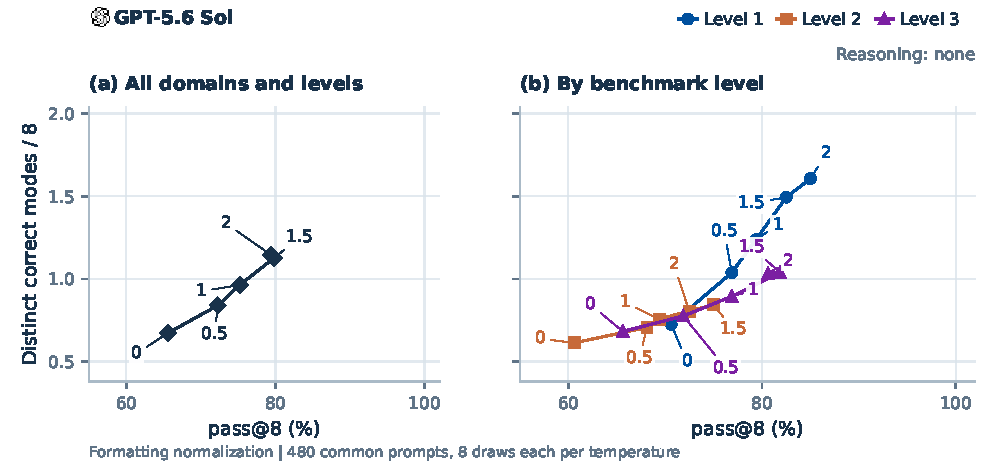
\includegraphics[width=.98\linewidth]{figures/gpt56_temperature_curve.pdf}
  \caption{\textbf{Nonzero temperatures yield greater observed eight-draw coverage.}
  GPT-5.6 Sol with reasoning \texttt{none}, typography normalization, and the same
  480 prompts at each of five temperatures (32 per domain--level cell, eight
  responses each). Left: an equal mean over all 15 domain--level cells; right:
  equal means over five domains at each level, identified by color and marker.
  The horizontal axis is empirical \texttt{pass@8}; the vertical axis averages
  distinct correct solution modes per eight responses, including unsolved prompts
  as zero. Labels give requested temperatures; segments connect measured point
  estimates in temperature order. Table~\ref{tab:gpt56-temperature} gives
  95\% whole-prompt bootstrap intervals. Mode counts depend on
  success and correct-answer variation and need not track \texttt{pass@8}.}
  \label{fig:gpt56-temperature-curve}
\end{figure}
}

\section{Comparison across Hosted Deployments}
\label{app:hosted-comparison}

Figure~\ref{fig:hosted-verified-breadth} compares accuracy and success-conditional
solution-mode diversity across hosted deployments. Its accuracy row uses a
common formatting normalizer and the revised Opus 5 \texttt{Python} instructions at
each level; hollow marks show that deployment's original \texttt{Python} condition.
Other accuracy cells use the original instructions. The diversity row uses
strict grades and original instructions for every deployment, with the
prompt-level estimand and eligibility criteria of App.~\ref{app:hosted-mode-diversity}.
Accuracy includes every response, including refusals and verification failures.
Provider settings differ, so the figure describes the stated configurations
rather than ranking models under matched prompts and compute.

The tables and \texttt{Graph} figure use the original instructions for every deployment.
The \texttt{Python} comparison reports both instruction conditions under strict and
formatting-normalized grading. Level 3 extends the evaluation beyond the
training levels, and difficulty need not increase with level for every hosted deployment.

\paragraph{Evaluation population.}
The deployments are GPT-5.6 Sol, Claude Opus 5, GPT-5.4, Grok 4.3, Kimi K3, Claude Opus 4.8, DeepSeek V4 Pro. The original-instruction cohort contains
107,520 responses: 15,360 per deployment, with the same 128 held-out
prompts in each of five domains and three levels, and eight stateless responses
per prompt. Requests use no model-side tools or conversation history, and
the evaluation includes no task training or replay intervention.

\paragraph{Provider configurations.}
All deployments request medium reasoning effort and an 8,192-token native
output limit. Claude Opus 5 and Claude Opus 4.8 use Anthropic Messages with
adaptive thinking; the other deployments use hosted API routes.

The requested reasoning setting and output limit do not match compute across
providers: effort labels and token accounting have provider-specific meanings.
Temperature and nucleus sampling use provider defaults, whose exact values
are unknown when the provider does not return them.

Strict grading checks the original executable answer; formatting-normalized
grading applies the same typography corrections across deployments before
the executable checks. The tables below report original-instruction results
under both grading rules. Prompt preferences and the Level-1 \texttt{PantryPlan}
interface difference limit comparisons across levels. \texttt{Countdown} has no uniform
reference, because its total support is not certified. This inference-only comparison does not identify a training
cause, a model-size effect, or a difficulty effect. Collision intervals are
pointwise estimates for individual cells, not intervals for paired deployment differences.

The 15,360 scored DeepSeek V4 Pro responses include verification failures
and truncations. Usage totals omit requests without reported usage and
therefore give only a lower bound on the true total cost of all attempted API requests.

\begin{figure}[!htbp]
  \centering
  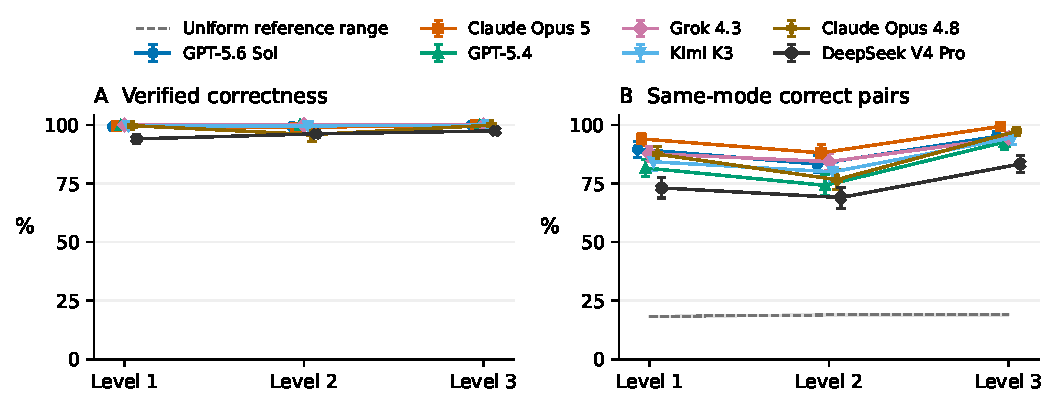
\includegraphics[width=\linewidth]{figures/frontier_comparison_20260911_graph.pdf}
  \caption{\textbf{Hosted \texttt{Graph} answers are usually correct but concentrated relative to uniform sampling.}
  Panel A shows strict per-response accuracy; panel B shows the fraction of
  correct pairs sharing a solution mode, pooling pairs across prompts. Colors
  and markers identify seven deployments, each with the same 128 prompts per
  level and eight stateless responses per prompt. Error bars are pointwise
  95\% intervals from resampling whole prompts. The gray band spans the
  deployments' uniform-correct-mode references, weighted by
  correct-pair counts; the dashed line is their mean. Level labels imply
  neither equal nor monotone difficulty across deployments.}
  \label{fig:hosted-graph-comparison}
\end{figure}

\subsection{A separate Python prompt sensitivity test}
\label{app:hosted-python-prompt}
After the original Opus 5 Python refusals, synthetic tasks were used to select
a direct arithmetic-expression formulation with no system message. We then
collected eight independent draws for every original Python test task: all
384 prompts across three levels, with unchanged adaptive thinking, medium
effort, 8,192 output tokens, allowed operators, public inputs and frozen graders.
The revised user instruction asks for a one-line boxed Python lambda returning
any proper divisor for each listed input. It does not prescribe a preferred divisor.
Both task wording and system-message presence change; collection time also differs.
This exploratory follow-up therefore supports a practical prompt repair without
isolating its cause. Original refusals and all three residual refusals are retained.
The original-protocol appendix tables retain all original Python responses;
the main display uses this complete revised condition with an explicit caption note.

\begin{table}[!htbp]
  \centering
  \caption{\textbf{Opus 5 Python: original versus plain task wording.}
  Each row has 1,024 responses. R counts native refusals; A is per-response accuracy (\%),
  D is \texttt{distinct@8}, and C is correct-pair collision (\%).
  Strict and normalized results use the same frozen grader and typography rule.
  Original Level-2/3 collision is undefined because no prompt has two correct draws.}
  \small
  \setlength{\tabcolsep}{4pt}
  \begin{tabular}{@{}llrrrrrrr@{}}
    \toprule
    & & & \multicolumn{3}{c}{Strict} & \multicolumn{3}{c}{Normalized} \\
    Condition & L & R & A & D & C & A & D & C \\
    \midrule
    Original & 1 & 409 & 38.1 & 0.91 & 93.0 & 60.0 & 1.12 & 90.4 \\
     & 2 & 1021 & 0.3 & 0.02 & -- & 0.3 & 0.02 & -- \\
     & 3 & 1024 & 0.0 & 0.00 & -- & 0.0 & 0.00 & -- \\
    \midrule
    Plain user, no system & 1 & 0 & 74.9 & 1.42 & 80.2 & 100.0 & 1.49 & 79.9 \\
     & 2 & 0 & 71.8 & 1.31 & 84.7 & 100.0 & 1.38 & 85.7 \\
     & 3 & 3 & 76.2 & 1.38 & 82.7 & 99.7 & 1.41 & 84.1 \\
    \bottomrule
  \end{tabular}
\end{table}

The new condition has no API failures or token-limit truncations. Strict grading
accepts 2,282 responses; the frozen rule rescues 787 more
by converting escaped percent signs (\verb|\%|) to Python modulo (\verb|%|).
Thus every non-refused answer passes after this formatting-only correction.
Normalized collision is 79.9/85.7/84.1\%, versus conditional uniform references
of 1.43/1.15/1.15\%. The residual three refusals occur on two prompts whose
other identical requests are accepted. No retry-until-accepted selection is used.

The paired analysis resamples whole eight-draw prompt groups across conditions
(20,000 replicates). Normalized accuracy gains at Levels 1/2/3 are
40.0 [34.7, 45.5], 99.7 [99.3, 100.0], and 99.7 [99.2, 100.0] percentage points
(pointwise 95\% intervals). Output draws themselves are independent, and the
different correct-pair populations preclude interpreting a raw collision
difference as a matched-population prompt effect.

The saved sensitivity record binds the original and revised native receipts,
request payloads, strict regrade audit and frozen normalization outputs.

\paragraph{Separate first-valid retry diagnostic.}
After completing the fixed 3,072-response revised-wording cohort, a separate
condition retries only its three remaining refused slots, retaining the
first verified-valid response. All three succeed on their first additional
request, and all reproduce a mode already seen for that prompt. This uses
3,075 requests to select 3,072 valid responses; its 100\% accepted-set
accuracy follows from selection and is not unconditional model accuracy.
The selected set's \texttt{distinct@8} is unchanged at 1.492, 1.375, 1.414 at
Levels 1--3. Level-3 correct-pair collision changes from 84.0909\% to 84.1518\%;
the other levels are unchanged. All initial and retry responses remain
preserved. The main figure continues to use the complete fixed eight-draw
condition, including its three refusals; these selected-validity results
are only a separate diagnostic with variable request effort.


\subsection{Requested-temperature sensitivity}
\label{app:hosted-temperature}
Grok 4.3 and Kimi K3 each receive requested temperatures $T=1.0$ and
$T=1.5$ on the same 120 tasks: eight prompts in each of five domains and
three levels. Eight responses from separate requests per prompt give 960
responses per deployment--temperature condition and 3,840 in total.
Within each deployment, the two conditions share all non-temperature
request settings and run concurrently. Accuracy and mode counts include
all responses, including verification failures and truncated outputs.

The providers accept both requested temperature settings, but their responses
do not report effective sampling temperatures. DeepSeek is outside this
comparison because its thinking-mode interface ignores the temperature setting.
The results concern these requested settings on this 120-task subset and
do not establish a general temperature response for all hosted deployments.

Each level summary averages five domains equally; All averages the 15
domain--level cells equally. Collision pools correct pairs within each cell,
so tasks with more correct responses receive more weight. Eligible tasks
and pair weights can differ between temperatures; the contrast does not
hold accuracy or the correct-pair population fixed. An undefined cell makes
the corresponding average undefined. Pointwise 95\% intervals use 20,000
paired whole-prompt bootstrap resamples, stratified by domain and level.
Each resampled prompt includes all eight responses. Prompts are paired
across conditions; output draws are not. Intervals have no multiplicity adjustment.

\paragraph{Observed sensitivity.}
For Grok, the observed diversity change is +0.050 [$-$0.058, +0.158] modes, and the collision change is $-$0.78 [$-$3.86, +2.12] percentage points. Both intervals include zero, so neither shows a clear diversity gain.
The per-response accuracy change is $-$2.29 [$-$3.85, $-$0.94] percentage points. These results do not establish invariance to temperature in general.

At $T=1.5$, 696 of Kimi's 960 outputs reach the token limit,
compared with 0 at $T=1.0$. Strict accuracy falls from 96.56\% to 21.25\%, while raw diversity falls from 1.933 to 0.983 modes.
The large increase in truncation accompanies losses in accuracy and distinct modes.
These results do not isolate correct-output concentration at matched accuracy.
The five-domain collision mean is undefined at
$T=1.5$ because some cells have no eligible correct pairs. Neither model
has provider-declared refusals in this experiment.

$\dagger$ marks a defined contrast whose interval is omitted because some
bootstrap resamples have undefined cells. Five-domain averages require all
five cell estimates; conditioning on only the estimable resamples would
change the uncertainty calculation.

\begin{table}[!htbp]
  \centering
  \setlength{\parfillskip}{0pt plus .20\linewidth}
  \caption{\textbf{Higher requested temperature yields no clear Grok diversity gain and much lower Kimi accuracy.} Strict executable grades compare $T=1.5$ with $T=1.0$.
  Each condition contains eight responses on each of 120 tasks.
  Level summaries average five domains equally; All averages 15 domain--level cells.
  A is per-response accuracy (\%); D is mean \texttt{distinct@8};
  C is correct-pair collision (\%), pooling pairs within each cell.
  Differences subtract $T=1.0$ from $T=1.5$: mode counts for D and percentage points for A/C.
  Brackets give pointwise 95\% intervals from paired whole-prompt bootstrap resampling.
  $\dagger$ marks an omitted interval when some resamples have undefined cells;
  -- denotes an undefined estimate or omitted interval.}
  \small
  \setlength{\tabcolsep}{5pt}
  \begin{tabular}{@{}llrrrr@{}}
    \toprule
    Deployment & Level & Metric & $T=1.0$ & $T=1.5$ & Difference [95\% interval] \\
    \midrule
    Grok 4.3 & 1 & A & 98.12 & 95.62 & $-$2.50 [$-$4.06, $-$0.94] \\
     &  & D & 1.900 & 2.000 & +0.100 [$-$0.100, +0.300] \\
     &  & C & 72.89 & 73.16 & +0.27 [$-$6.31, +6.37] \\
     & 2 & A & 99.06 & 99.38 & +0.31 [$-$0.94, +1.56] \\
     &  & D & 1.425 & 1.425 & +0.000 [$-$0.175, +0.200] \\
     &  & C & 86.61 & 85.20 & $-$1.41 [$-$6.26, +3.30] \\
     & 3 & A & 98.75 & 94.06 & $-$4.69 [$-$9.06, $-$0.94] \\
     &  & D & 1.500 & 1.550 & +0.050 [$-$0.125, +0.225] \\
     &  & C & 84.04 & 82.85 & $-$1.20 [$-$5.48, +2.79] \\
     & All & A & 98.65 & 96.35 & $-$2.29 [$-$3.85, $-$0.94] \\
     &  & D & 1.608 & 1.658 & +0.050 [$-$0.058, +0.158] \\
     &  & C & 81.18 & 80.40 & $-$0.78 [$-$3.86, +2.12] \\
    \midrule
    Kimi K3 & 1 & A & 92.50 & 22.50 & $-$70.00 [$-$75.62, $-$63.75] \\
     &  & D & 2.200 & 1.075 & $-$1.125 [$-$1.475, $-$0.775] \\
     &  & C & 66.23 & 53.12 & $-$13.11 [--]$^\dagger$ \\
     & 2 & A & 98.12 & 20.31 & $-$77.81 [$-$82.50, $-$72.81] \\
     &  & D & 1.850 & 0.900 & $-$0.950 [$-$1.300, $-$0.625] \\
     &  & C & 72.18 & 66.55 & $-$5.63 [--]$^\dagger$ \\
     & 3 & A & 99.06 & 20.94 & $-$78.12 [$-$83.75, $-$72.81] \\
     &  & D & 1.750 & 0.975 & $-$0.775 [$-$1.025, $-$0.525] \\
     &  & C & 78.33 & -- & -- \\
     & All & A & 96.56 & 21.25 & $-$75.31 [$-$78.44, $-$72.19] \\
     &  & D & 1.933 & 0.983 & $-$0.950 [$-$1.133, $-$0.767] \\
     &  & C & 72.25 & -- & -- \\
    \bottomrule
  \end{tabular}
\end{table}

\begin{table}[!htbp]
  \centering
  \setlength{\parfillskip}{0pt plus .20\linewidth}
  \caption{\textbf{Formatting normalization leaves the temperature sensitivity largely unchanged.} Only rows differing from strict grading appear; all other rows are identical.
  Each condition contains eight responses on each of 120 tasks.
  Level summaries average five domains equally; All averages 15 domain--level cells.
  A is per-response accuracy (\%); D is mean \texttt{distinct@8};
  C is correct-pair collision (\%), pooling pairs within each cell.
  Differences subtract $T=1.0$ from $T=1.5$: mode counts for D and percentage points for A/C.
  Brackets give pointwise 95\% intervals from paired whole-prompt bootstrap resampling.
  $\dagger$ marks an omitted interval when some resamples have undefined cells;
  -- denotes an undefined estimate or omitted interval.}
  \small
  \setlength{\tabcolsep}{5pt}
  \begin{tabular}{@{}llrrrr@{}}
    \toprule
    Deployment & Level & Metric & $T=1.0$ & $T=1.5$ & Difference [95\% interval] \\
    \midrule
    Kimi K3 & 1 & A & 92.50 & 22.81 & $-$69.69 [$-$75.31, $-$63.44] \\
     & 1 & C & 66.23 & 53.61 & $-$12.62 [--]$^\dagger$ \\
     & 3 & A & 99.38 & 20.94 & $-$78.44 [$-$84.06, $-$73.12] \\
     & 3 & C & 78.18 & -- & -- \\
     & All & A & 96.67 & 21.35 & $-$75.31 [$-$78.44, $-$72.19] \\
     & All & C & 72.20 & -- & -- \\
    \bottomrule
  \end{tabular}
\end{table}

Across the hosted comparisons, \texttt{Countdown} has no uniform reference because its
total support is not certified, so uniform-reference comparisons use the other
four domains. Cross-level differences
also reflect different task populations and do not establish a common ordering
of model difficulty. These inference-only results do not identify a training
or parameter-scale cause of concentration.


\subsection{GPT-5.6 Sol: temperature, pass@8 and verified modes}
\label{app:gpt56-temperature}
Figure~\ref{fig:gpt56-temperature-curve} plots empirical \texttt{pass@8}
against \texttt{distinct@8} for $T\in\{0.0,0.5,1.0,1.5,2.0\}$, with reasoning
\texttt{none}. Each condition uses the same 480 held-out prompts
(32 per domain--level cell), with eight stateless responses per prompt:
3,840 responses per temperature and 19,200 in total. A prompt contributes one
to \texttt{pass@8} if at least one of its eight answers is verified correct,
and contributes its number of distinct correct canonical keys to \texttt{distinct@8}.
Both metrics average over all prompts, including those with no correct answer.
The empirical \texttt{pass@8} uses the observed eight-response groups;
$1-(1-p)^8$ applied to pooled accuracy would ignore differences among prompts.
Raw \texttt{distinct@8} depends on both success and variation among correct
solution modes, so its changes need not track \texttt{pass@8}.

Prompts are selected independently of model outputs within each
domain--level cell. The evaluation comprises 120-prompt and 360-prompt
subsets collected at different times. Temperatures are interleaved for the
360-prompt subset; zero and nonzero temperatures are collected separately
for the 120-prompt subset. Service changes can therefore confound temperature
contrasts, and prompt composition can affect comparisons between subsets.

Requests use the same prompt wording, verifiers and sampling controls
except temperature, with an 8,192-token output cap. Returned metadata
identifies \texttt{gpt-5.6-sol-2026-07-09}, reasoning \texttt{none},
$\texttt{top\_p}=0.98$ and the requested temperature in every condition.
The exposed settings do not establish unchanged internal service behavior
or independent provider randomness. A zero-temperature request does not
establish deterministic outputs. The deployment rejects non-default
temperatures with medium reasoning and rejects temperature 2.5; this
sweep therefore does not test temperature robustness under medium reasoning.

Strict grading applies the executable validators directly. Normalized
grading uses the typography rules in App.~\ref{app:hosted-concentration}
before the same validators, preserving strict successes and their mode keys.

Each level averages five domains equally; All averages all 15 cells.
Pointwise 95\% intervals use 20,000 paired whole-prompt bootstrap
resamples stratified by domain and level, keeping all eight responses
together and matching prompts across temperatures. Individual model
responses are not paired across conditions.
There is no multiplicity adjustment. A zero-width empirical interval
reflects constant observed groups, not certain success on unseen prompts.

\begin{table}[!htbp]
\centering
\setlength{\parfillskip}{0pt plus .20\linewidth}
\caption{\textbf{Nonzero temperatures improve eight-draw coverage in this sweep.}
P is solved prompts (\%, \texttt{pass@8}); D is \texttt{distinct@8};
A is per-response accuracy (\%). G is the grading: S strict,
N formatting-normalized. Each temperature uses the same 480 prompts
(32 per domain--level cell), eight responses each, and reasoning \texttt{none}.
Level rows average five domains equally; All averages all 15 cells.
Brackets give pointwise 95\% whole-prompt bootstrap intervals.}
\label{tab:gpt56-temperature}
\small
\setlength{\tabcolsep}{4pt}
\begin{tabular}{@{}lllrrr@{}}
\toprule
$T$ & Level & G & P [95\% interval] & D [95\% interval] & A [95\% interval] \\
\midrule
0.0 & 1 & S & 55.0 [48.8, 61.3] & 0.569 [0.500, 0.637] & 53.9 [47.7, 60.1] \\
 & 2 &  & 45.0 [39.4, 50.6] & 0.456 [0.400, 0.512] & 39.5 [34.4, 44.7] \\
 & 3 &  & 49.4 [42.5, 56.2] & 0.519 [0.444, 0.594] & 44.5 [38.3, 50.9] \\
 & All &  & 49.8 [46.2, 53.3] & 0.515 [0.475, 0.554] & 46.0 [42.6, 49.4] \\
0.5 & 1 & S & 70.6 [64.4, 76.9] & 0.956 [0.850, 1.069] & 57.5 [51.9, 63.0] \\
 & 2 &  & 50.0 [44.4, 55.6] & 0.525 [0.463, 0.594] & 38.6 [33.9, 43.4] \\
 & 3 &  & 54.4 [48.1, 60.6] & 0.581 [0.506, 0.662] & 43.0 [37.1, 48.9] \\
 & All &  & 58.3 [54.8, 61.9] & 0.688 [0.640, 0.738] & 46.4 [43.3, 49.5] \\
1.0 & 1 & S & 75.6 [69.4, 81.2] & 1.181 [1.050, 1.312] & 57.3 [52.0, 62.7] \\
 & 2 &  & 51.9 [45.6, 58.1] & 0.581 [0.506, 0.662] & 37.6 [33.2, 42.0] \\
 & 3 &  & 60.6 [54.4, 66.9] & 0.713 [0.625, 0.806] & 42.7 [37.3, 48.1] \\
 & All &  & 62.7 [59.2, 66.2] & 0.825 [0.767, 0.885] & 45.9 [42.9, 48.8] \\
1.5 & 1 & S & 80.6 [75.0, 86.2] & 1.413 [1.269, 1.556] & 56.6 [51.7, 61.4] \\
 & 2 &  & 58.1 [51.9, 64.4] & 0.650 [0.569, 0.738] & 38.4 [34.3, 42.7] \\
 & 3 &  & 65.6 [59.4, 71.2] & 0.838 [0.731, 0.956] & 43.0 [38.0, 48.2] \\
 & All &  & 68.1 [64.8, 71.5] & 0.967 [0.900, 1.035] & 46.0 [43.3, 48.8] \\
2.0 & 1 & S & 83.8 [78.1, 88.8] & 1.519 [1.375, 1.663] & 59.7 [54.8, 64.5] \\
 & 2 &  & 54.4 [48.1, 60.6] & 0.600 [0.525, 0.675] & 35.3 [31.4, 39.3] \\
 & 3 &  & 61.9 [56.2, 67.5] & 0.819 [0.719, 0.925] & 40.5 [35.8, 45.5] \\
 & All &  & 66.7 [63.3, 70.0] & 0.979 [0.915, 1.044] & 45.2 [42.6, 47.8] \\
\midrule
0.0 & 1 & N & 70.6 [65.0, 76.2] & 0.725 [0.662, 0.788] & 70.5 [64.5, 76.2] \\
 & 2 &  & 60.6 [55.0, 66.2] & 0.613 [0.556, 0.669] & 54.5 [49.0, 59.9] \\
 & 3 &  & 65.6 [59.4, 71.9] & 0.681 [0.606, 0.756] & 61.4 [55.2, 67.6] \\
 & All &  & 65.6 [62.3, 69.0] & 0.673 [0.635, 0.710] & 62.1 [58.8, 65.5] \\
0.5 & 1 & N & 76.9 [71.2, 82.5] & 1.038 [0.931, 1.150] & 71.7 [66.4, 77.0] \\
 & 2 &  & 68.1 [62.5, 73.8] & 0.706 [0.644, 0.769] & 53.7 [48.8, 58.6] \\
 & 3 &  & 71.9 [65.6, 77.5] & 0.775 [0.700, 0.850] & 58.1 [52.3, 63.9] \\
 & All &  & 72.3 [69.2, 75.4] & 0.840 [0.792, 0.890] & 61.2 [58.2, 64.3] \\
1.0 & 1 & N & 79.4 [73.8, 84.4] & 1.238 [1.106, 1.369] & 70.4 [65.2, 75.5] \\
 & 2 &  & 69.4 [63.7, 75.0] & 0.756 [0.681, 0.831] & 51.6 [47.1, 56.2] \\
 & 3 &  & 76.9 [71.2, 82.5] & 0.894 [0.806, 0.988] & 55.2 [49.8, 60.7] \\
 & All &  & 75.2 [72.1, 78.3] & 0.963 [0.904, 1.021] & 59.1 [56.2, 62.0] \\
1.5 & 1 & N & 82.5 [77.5, 87.5] & 1.494 [1.344, 1.644] & 68.5 [63.7, 73.3] \\
 & 2 &  & 75.0 [69.4, 80.6] & 0.844 [0.762, 0.931] & 49.8 [45.5, 54.3] \\
 & 3 &  & 81.9 [76.2, 87.5] & 1.038 [0.931, 1.156] & 54.7 [49.6, 59.8] \\
 & All &  & 79.8 [76.7, 82.9] & 1.125 [1.056, 1.196] & 57.7 [54.9, 60.5] \\
2.0 & 1 & N & 85.0 [80.0, 90.0] & 1.606 [1.456, 1.762] & 69.6 [64.8, 74.3] \\
 & 2 &  & 72.5 [66.9, 78.1] & 0.800 [0.731, 0.869] & 45.7 [41.7, 49.8] \\
 & 3 &  & 80.6 [75.0, 86.2] & 1.031 [0.931, 1.137] & 52.5 [47.7, 57.5] \\
 & All &  & 79.4 [76.2, 82.5] & 1.146 [1.079, 1.212] & 55.9 [53.3, 58.6] \\
\bottomrule
\end{tabular}
\end{table}

\paragraph{Coverage and sampled solution modes.}
At $T=0.0$ and $T=2.0$, normalized \texttt{pass@8} is 65.62\% and 79.38\%, respectively,
while \texttt{distinct@8} is 0.673 and 1.146.
Across these five measured temperatures, the highest observed aggregate
\texttt{pass@8} occurs at $T=1.5$ and the highest \texttt{distinct@8}
occurs at $T=2.0$. These five temperatures do not establish
a population optimum or a continuous Pareto boundary, and level-specific curves differ.

Per-response accuracy changes from 62.11\% to 55.94\% between the endpoints.
That diagnostic is distinct from \texttt{pass@8}: success within eight
draws and the reliability of an individual draw need not change together as temperature varies.

The paired $T=2.0$ minus $T=0.0$ contrast is 13.8 [10.8, 16.7] \texttt{pass@8} percentage points and 0.473 [0.417, 0.529] distinct correct modes, with pointwise 95\% intervals.

\paragraph{Response outcomes.}
At every temperature, none of the 3,840 outputs is token-limited or a provider-declared refusal.
Unsuccessful answers remain in the eight-response groups.

\paragraph{Sensitivity across prompt subsets.}
We compare the same temperature contrast within each prompt subset.
The subsets differ in prompts and collection periods, so differences
between them do not isolate a causal effect of time. Brackets are
pointwise 95\% intervals.

Across all 480 prompts, the paired $T=2$ minus $T=1.5$ contrast is $-$0.4 [$-$2.5, 1.7] \texttt{pass@8} percentage points and 0.021 [$-$0.029, 0.071] distinct modes.
In the 120-prompt subset it is $-$1.7 [$-$5.0, 0.8] points and $-$0.008 [$-$0.083, 0.067] modes, and in the 360-prompt subset it is 0.0 [$-$2.8, 2.8] points and 0.031 [$-$0.033, 0.094] modes.

\subsection{Native provider outcomes and undefined concentration}
\label{app:hosted-provider-outcomes}
Provider metadata distinguish refusal and filtering from executable correctness.
A refusal does not establish that the underlying model cannot solve the task.
Classification uses native stop reasons, refusal fields and filter metadata;
it does not detect refusals expressed only in ordinary answer text.
An empty visible answer is a failed draw, including when the response contains
reasoning output. Empty-answer and refusal counts therefore need not agree.

Correct-pair collision requires at least two correct draws on one prompt.
It is undefined otherwise, as is a five-domain mean containing any undefined
domain. Dashes denote these undefined values. Accuracy and distinct-mode
counts include all responses, with zero correct modes on unsuccessful prompts.

Native completion states over the 15,360 original-instruction responses per deployment are:

\begin{itemize}\setlength{\itemsep}{0pt}
\item GPT-5.6 Sol --- completed: 15,360
\item Claude Opus 5 --- end\_turn: 12,838, refusal: 2,522
\item GPT-5.4 --- completed: 15,355, incomplete: 5
\item Grok 4.3 --- stop: 15,360
\item Kimi K3 --- length: 15, stop: 15,345
\item Claude Opus 4.8 --- end\_turn: 15,355, max\_tokens: 5
\item DeepSeek V4 Pro --- length: 632, stop: 14,728
\end{itemize}

Claude Opus 5 returns provider-declared refusals for 409, 1,021 and 1,024 of the 1,024 \texttt{Python} requests at Levels 1, 2 and 3, respectively.
The provider assigns them the refusal category cyber (2,454). These labels describe service behavior on factor-selection tasks;
they do not measure concentration among correct \texttt{Python} outputs.

\begin{table}[!htbp]
  \centering
  \caption{\textbf{Provider-declared refusals occur only for Opus 5 in this cohort.} Each original-instruction cell contains 128 prompts with eight responses each (1,024 responses). R counts native refusal signals, F native content filters, and E responses without visible answer text, including reasoning-only outputs. Counters can overlap and are separate from executable grades. Only cells with a nonzero counter appear; the other 83 of 105 cells have $R=F=E=0$, including all cells for GPT-5.6 Sol, Grok 4.3 and Kimi K3. Zero R does not exclude refusals expressed only in answer text.}
  \label{tab:hosted-provider-outcomes}
  \small
  \setlength{\tabcolsep}{5pt}
  \begin{tabular}{@{}llrrrr@{}}
    \toprule
    \textbf{Deployment} & \textbf{L} & \textbf{Domain} &
      \textbf{R} & \textbf{F} & \textbf{E} \\
    \midrule
    Claude Opus 5 & 1 & \texttt{Python} & 409 & 0 & 409 \\
     & 2 & \texttt{Python} & 1021 & 0 & 1021 \\
     & 2 & \texttt{MathIR} & 35 & 0 & 35 \\
     & 3 & \texttt{Python} & 1024 & 0 & 1024 \\
     & 3 & \texttt{MathIR} & 33 & 0 & 32 \\
    GPT-5.4 & 1 & \texttt{PantryPlan} & 0 & 0 & 1 \\
     & 2 & \texttt{Countdown} & 0 & 0 & 1 \\
     & 3 & \texttt{Countdown} & 0 & 0 & 1 \\
     & 3 & \texttt{PantryPlan} & 0 & 0 & 2 \\
    Claude Opus 4.8 & 3 & \texttt{Countdown} & 0 & 0 & 3 \\
     & 3 & \texttt{PantryPlan} & 0 & 0 & 1 \\
    DeepSeek V4 Pro & 1 & \texttt{Graph} & 0 & 0 & 59 \\
     & 1 & \texttt{MathIR} & 0 & 0 & 4 \\
     & 1 & \texttt{PantryPlan} & 0 & 0 & 13 \\
     & 2 & \texttt{Graph} & 0 & 0 & 38 \\
     & 2 & \texttt{Countdown} & 0 & 0 & 1 \\
     & 2 & \texttt{MathIR} & 0 & 0 & 59 \\
     & 2 & \texttt{PantryPlan} & 0 & 0 & 80 \\
     & 3 & \texttt{Graph} & 0 & 0 & 24 \\
     & 3 & \texttt{Countdown} & 0 & 0 & 7 \\
     & 3 & \texttt{MathIR} & 0 & 0 & 100 \\
     & 3 & \texttt{PantryPlan} & 0 & 0 & 246 \\
    \bottomrule
  \end{tabular}
\end{table}



\begin{table}[!htbp]
  \centering
  \caption{\textbf{Hosted deployments average fewer than three distinct correct modes per prompt.}
  Each row averages five domains equally under strict grading and original
  instructions, with 128 prompts per domain and eight responses per prompt.
  M/P are \texttt{mean@8}/\texttt{pass@8} (\%); D averages distinct correct
  solution modes, including zeros. C is correct-pair collision (\%), pooling
  pairs within each domain before averaging domains. Pointwise 95\% intervals
  use 2,000 whole-prompt bootstrap resamples within domains. A dash denotes
  an undefined domain collision and hence an undefined five-domain mean.
  Provider settings differ, so these are descriptive deployment comparisons.}
  \small
  \setlength{\tabcolsep}{3pt}
  \begin{tabular}{@{}lrrrrr@{}}
    \toprule
    Deployment & Level & M & P & D & C (95\% interval) \\
    \midrule
    GPT-5.6 Sol & 1 & 83.0 & 95.8 & 1.71 & 74.0 [71.9, 76.1] \\
GPT-5.6 Sol & 2 & 62.9 & 77.5 & 1.16 & 82.3 [80.3, 84.4] \\
GPT-5.6 Sol & 3 & 68.7 & 80.3 & 1.18 & 84.5 [82.8, 86.2] \\
\midrule
Claude Opus 5 & 1 & 85.3 & 94.5 & 1.32 & 86.3 [84.5, 88.0] \\
Claude Opus 5 & 2 & 76.6 & 80.2 & 1.16 & -- \\
Claude Opus 5 & 3 & 77.8 & 79.8 & 1.07 & -- \\
\midrule
GPT-5.4 & 1 & 93.7 & 98.1 & 2.09 & 67.2 [65.1, 69.3] \\
GPT-5.4 & 2 & 80.6 & 97.7 & 1.61 & 74.7 [72.4, 76.8] \\
GPT-5.4 & 3 & 83.3 & 97.8 & 1.57 & 78.8 [76.9, 80.7] \\
\midrule
Grok 4.3 & 1 & 98.3 & 99.5 & 1.97 & 72.4 [70.7, 74.0] \\
Grok 4.3 & 2 & 99.3 & 100.0 & 1.57 & 82.1 [80.6, 83.7] \\
Grok 4.3 & 3 & 98.8 & 100.0 & 1.55 & 83.0 [81.5, 84.6] \\
\midrule
Kimi K3 & 1 & 96.9 & 98.4 & 2.31 & 62.5 [60.6, 64.4] \\
Kimi K3 & 2 & 96.8 & 100.0 & 2.05 & 69.4 [67.6, 71.2] \\
Kimi K3 & 3 & 97.8 & 100.0 & 1.90 & 74.6 [73.1, 76.2] \\
\midrule
Claude Opus 4.8 & 1 & 96.4 & 98.8 & 1.64 & 78.4 [76.6, 80.3] \\
Claude Opus 4.8 & 2 & 98.5 & 100.0 & 1.67 & 77.2 [75.4, 79.1] \\
Claude Opus 4.8 & 3 & 98.9 & 99.8 & 1.51 & 83.4 [81.8, 84.9] \\
\midrule
DeepSeek V4 Pro & 1 & 96.4 & 98.4 & 2.01 & 71.0 [69.4, 72.7] \\
DeepSeek V4 Pro & 2 & 93.7 & 99.1 & 1.84 & 68.7 [67.0, 70.3] \\
DeepSeek V4 Pro & 3 & 91.0 & 99.7 & 1.62 & 78.8 [76.9, 80.9] \\
\bottomrule

  \end{tabular}
\end{table}

\begin{table}[!htbp]
  \centering
  \caption{\textbf{GPT-5.6 Sol: Strict executable grades.} Each cell has 128 prompts and 1,024 responses. M/P denote \texttt{mean@8}/\texttt{pass@8} (\%); D is \texttt{distinct@8}. C is correct-pair collision (\%) with pointwise 95\% prompt-bootstrap intervals. U is its conditional uniform reference (\%).}
  \small
  \setlength{\tabcolsep}{4pt}
  \begin{tabular}{@{}rlrrrrr@{}}
    \toprule
    Level & Domain & M & P & D & C (95\% interval) & U \\
    \midrule
    1 & Graph & 99.2 & 100.0 & 1.30 & 89.7 [86.3, 92.8] & 18.3 \\
    1 & Countdown & 86.1 & 98.4 & 1.77 & 71.2 [66.1, 75.9] & -- \\
    1 & Python & 40.4 & 90.6 & 1.11 & 81.8 [76.9, 87.2] & 0.8 \\
    1 & MathIR & 89.3 & 89.8 & 1.38 & 80.3 [75.4, 85.0] & 20.0 \\
    1 & PantryPlan & 100.0 & 100.0 & 3.00 & 46.9 [42.2, 51.5] & 6.5 \\
    \midrule
    2 & Graph & 99.3 & 100.0 & 1.48 & 83.3 [79.6, 87.0] & 18.9 \\
    2 & Countdown & 65.4 & 86.7 & 1.57 & 64.7 [59.0, 70.6] & -- \\
    2 & Python & 8.5 & 11.7 & 0.12 & 100.0 [100.0, 100.0] & 0.7 \\
    2 & MathIR & 86.2 & 93.0 & 0.93 & 100.0 [100.0, 100.0] & 20.0 \\
    2 & PantryPlan & 55.3 & 96.1 & 1.72 & 63.6 [56.8, 70.3] & 6.9 \\
    \midrule
    3 & Graph & 100.0 & 100.0 & 1.16 & 95.1 [92.4, 97.3] & 19.0 \\
    3 & Countdown & 71.2 & 89.8 & 1.38 & 76.4 [71.1, 81.8] & -- \\
    3 & Python & 9.4 & 14.1 & 0.14 & 100.0 [100.0, 100.0] & 0.9 \\
    3 & MathIR & 97.7 & 97.7 & 0.98 & 100.0 [100.0, 100.0] & 20.0 \\
    3 & PantryPlan & 65.3 & 100.0 & 2.22 & 51.0 [45.3, 57.3] & 6.8 \\
    \bottomrule
  \end{tabular}
\end{table}

\begin{table}[!htbp]
  \centering
  \caption{\textbf{Claude Opus 5: Strict executable grades.} Each cell has 128 prompts and 1,024 responses. M/P denote \texttt{mean@8}/\texttt{pass@8} (\%); D is \texttt{distinct@8}. C is correct-pair collision (\%) with pointwise 95\% prompt-bootstrap intervals. U is its conditional uniform reference (\%).}
  \small
  \setlength{\tabcolsep}{4pt}
  \begin{tabular}{@{}rlrrrrr@{}}
    \toprule
    Level & Domain & M & P & D & C (95\% interval) & U \\
    \midrule
    1 & Graph & 99.5 & 100.0 & 1.15 & 94.0 [91.3, 96.4] & 18.3 \\
    1 & Countdown & 100.0 & 100.0 & 1.59 & 78.8 [74.6, 83.0] & -- \\
    1 & Python & 38.1 & 81.2 & 0.91 & 93.0 [88.7, 96.6] & 0.7 \\
    1 & MathIR & 90.5 & 91.4 & 1.09 & 92.2 [88.8, 95.4] & 20.0 \\
    1 & PantryPlan & 98.4 & 100.0 & 1.86 & 73.5 [68.5, 78.2] & 6.5 \\
    \midrule
    2 & Graph & 98.9 & 100.0 & 1.32 & 88.1 [84.5, 91.6] & 18.9 \\
    2 & Countdown & 100.0 & 100.0 & 1.81 & 69.3 [65.2, 73.6] & -- \\
    2 & Python & 0.3 & 2.3 & 0.02 & -- & -- \\
    2 & MathIR & 89.1 & 98.4 & 1.06 & 96.5 [93.9, 98.6] & 20.0 \\
    2 & PantryPlan & 94.5 & 100.0 & 1.56 & 80.7 [76.0, 85.3] & 6.4 \\
    \midrule
    3 & Graph & 100.0 & 100.0 & 1.02 & 99.4 [98.3, 100.0] & 19.0 \\
    3 & Countdown & 99.9 & 100.0 & 1.66 & 76.2 [71.7, 80.7] & -- \\
    3 & Python & 0.0 & 0.0 & 0.00 & -- & -- \\
    3 & MathIR & 95.3 & 99.2 & 1.02 & 98.8 [97.5, 99.8] & 20.0 \\
    3 & PantryPlan & 93.6 & 100.0 & 1.63 & 78.8 [74.2, 83.4] & 6.5 \\
    \bottomrule
  \end{tabular}
\end{table}

\begin{table}[!htbp]
  \centering
  \caption{\textbf{GPT-5.4: Strict executable grades.} Each cell has 128 prompts and 1,024 responses. M/P denote \texttt{mean@8}/\texttt{pass@8} (\%); D is \texttt{distinct@8}. C is correct-pair collision (\%) with pointwise 95\% prompt-bootstrap intervals. U is its conditional uniform reference (\%).}
  \small
  \setlength{\tabcolsep}{4pt}
  \begin{tabular}{@{}rlrrrrr@{}}
    \toprule
    Level & Domain & M & P & D & C (95\% interval) & U \\
    \midrule
    1 & Graph & 99.8 & 100.0 & 1.57 & 81.6 [77.8, 85.4] & 18.3 \\
    1 & Countdown & 91.8 & 100.0 & 1.73 & 76.6 [71.2, 81.3] & -- \\
    1 & Python & 87.6 & 100.0 & 2.52 & 56.4 [51.3, 61.5] & 1.4 \\
    1 & MathIR & 89.3 & 90.6 & 1.45 & 78.6 [74.0, 83.4] & 20.0 \\
    1 & PantryPlan & 99.9 & 100.0 & 3.16 & 42.8 [38.4, 47.4] & 6.5 \\
    \midrule
    2 & Graph & 99.9 & 100.0 & 1.74 & 74.2 [69.8, 78.7] & 19.0 \\
    2 & Countdown & 91.1 & 100.0 & 1.98 & 63.0 [58.6, 67.5] & -- \\
    2 & Python & 47.9 & 96.1 & 1.47 & 72.9 [64.6, 80.2] & 1.0 \\
    2 & MathIR & 87.0 & 92.2 & 0.92 & 100.0 [100.0, 100.0] & 20.0 \\
    2 & PantryPlan & 77.0 & 100.0 & 1.93 & 63.2 [58.4, 68.6] & 6.8 \\
    \midrule
    3 & Graph & 99.8 & 100.0 & 1.23 & 92.7 [89.7, 95.4] & 19.0 \\
    3 & Countdown & 82.2 & 93.8 & 1.72 & 69.1 [64.4, 73.5] & -- \\
    3 & Python & 50.1 & 97.7 & 1.58 & 74.4 [68.6, 79.8] & 1.1 \\
    3 & MathIR & 97.7 & 97.7 & 0.98 & 100.0 [100.0, 100.0] & 20.0 \\
    3 & PantryPlan & 86.5 & 100.0 & 2.34 & 57.8 [52.8, 63.4] & 6.6 \\
    \bottomrule
  \end{tabular}
\end{table}

\begin{table}[!htbp]
  \centering
  \caption{\textbf{Grok 4.3: Strict executable grades.} Each cell has 128 prompts and 1,024 responses. M/P denote \texttt{mean@8}/\texttt{pass@8} (\%); D is \texttt{distinct@8}. C is correct-pair collision (\%) with pointwise 95\% prompt-bootstrap intervals. U is its conditional uniform reference (\%).}
  \small
  \setlength{\tabcolsep}{4pt}
  \begin{tabular}{@{}rlrrrrr@{}}
    \toprule
    Level & Domain & M & P & D & C (95\% interval) & U \\
    \midrule
    1 & Graph & 100.0 & 100.0 & 1.40 & 87.8 [84.2, 91.0] & 18.3 \\
    1 & Countdown & 99.9 & 100.0 & 2.05 & 64.8 [60.1, 69.5] & -- \\
    1 & Python & 99.8 & 100.0 & 1.41 & 88.0 [84.8, 91.0] & 1.4 \\
    1 & MathIR & 92.4 & 97.7 & 1.24 & 90.1 [86.9, 93.1] & 20.0 \\
    1 & PantryPlan & 99.4 & 100.0 & 3.77 & 31.4 [27.8, 35.1] & 6.5 \\
    \midrule
    2 & Graph & 99.9 & 100.0 & 1.52 & 84.3 [80.5, 88.0] & 19.0 \\
    2 & Countdown & 99.8 & 100.0 & 1.99 & 65.8 [61.8, 70.2] & -- \\
    2 & Python & 99.8 & 100.0 & 1.05 & 98.8 [97.8, 99.6] & 1.1 \\
    2 & MathIR & 97.5 & 100.0 & 1.12 & 94.9 [92.4, 97.2] & 20.0 \\
    2 & PantryPlan & 99.5 & 100.0 & 2.16 & 66.6 [61.2, 71.4] & 6.5 \\
    \midrule
    3 & Graph & 100.0 & 100.0 & 1.17 & 94.5 [92.0, 96.8] & 19.0 \\
    3 & Countdown & 99.9 & 100.0 & 1.98 & 66.3 [61.7, 71.0] & -- \\
    3 & Python & 99.9 & 100.0 & 1.04 & 98.6 [97.2, 99.6] & 1.2 \\
    3 & MathIR & 95.0 & 100.0 & 1.05 & 97.8 [95.9, 99.3] & 20.0 \\
    3 & PantryPlan & 99.2 & 100.0 & 2.52 & 58.0 [53.1, 63.5] & 6.5 \\
    \bottomrule
  \end{tabular}
\end{table}

\begin{table}[!htbp]
  \centering
  \caption{\textbf{Kimi K3: Strict executable grades.} Each cell has 128 prompts and 1,024 responses. M/P denote \texttt{mean@8}/\texttt{pass@8} (\%); D is \texttt{distinct@8}. C is correct-pair collision (\%) with pointwise 95\% prompt-bootstrap intervals. U is its conditional uniform reference (\%).}
  \small
  \setlength{\tabcolsep}{4pt}
  \begin{tabular}{@{}rlrrrrr@{}}
    \toprule
    Level & Domain & M & P & D & C (95\% interval) & U \\
    \midrule
    1 & Graph & 99.5 & 100.0 & 1.48 & 84.3 [80.4, 87.8] & 18.3 \\
    1 & Countdown & 99.1 & 100.0 & 1.91 & 68.4 [63.8, 73.3] & -- \\
    1 & Python & 97.9 & 100.0 & 2.52 & 57.7 [53.5, 61.9] & 1.4 \\
    1 & MathIR & 90.2 & 92.2 & 1.47 & 75.8 [70.7, 80.7] & 20.0 \\
    1 & PantryPlan & 97.5 & 100.0 & 4.18 & 26.2 [23.1, 29.2] & 6.5 \\
    \midrule
    2 & Graph & 99.6 & 100.0 & 1.62 & 80.0 [76.0, 84.1] & 19.0 \\
    2 & Countdown & 98.4 & 100.0 & 1.98 & 64.4 [59.9, 68.7] & -- \\
    2 & Python & 98.2 & 100.0 & 2.44 & 61.9 [57.6, 66.2] & 1.1 \\
    2 & MathIR & 94.3 & 100.0 & 1.02 & 99.8 [99.3, 100.0] & 20.0 \\
    2 & PantryPlan & 93.3 & 100.0 & 3.20 & 41.3 [36.6, 45.9] & 6.6 \\
    \midrule
    3 & Graph & 99.9 & 100.0 & 1.19 & 94.6 [91.8, 96.9] & 19.0 \\
    3 & Countdown & 97.5 & 100.0 & 1.84 & 70.6 [66.1, 74.8] & -- \\
    3 & Python & 98.0 & 100.0 & 2.34 & 64.7 [60.1, 69.0] & 1.2 \\
    3 & MathIR & 98.1 & 100.0 & 1.00 & 100.0 [100.0, 100.0] & 20.0 \\
    3 & PantryPlan & 95.6 & 100.0 & 3.13 & 43.4 [38.6, 48.3] & 6.5 \\
    \bottomrule
  \end{tabular}
\end{table}

\begin{table}[!htbp]
  \centering
  \caption{\textbf{Claude Opus 4.8: Strict executable grades.} Each cell has 128 prompts and 1,024 responses. M/P denote \texttt{mean@8}/\texttt{pass@8} (\%); D is \texttt{distinct@8}. C is correct-pair collision (\%) with pointwise 95\% prompt-bootstrap intervals. U is its conditional uniform reference (\%).}
  \small
  \setlength{\tabcolsep}{4pt}
  \begin{tabular}{@{}rlrrrrr@{}}
    \toprule
    Level & Domain & M & P & D & C (95\% interval) & U \\
    \midrule
    1 & Graph & 99.7 & 100.0 & 1.34 & 87.5 [83.9, 91.0] & 18.3 \\
    1 & Countdown & 95.6 & 99.2 & 1.78 & 69.8 [64.9, 74.5] & -- \\
    1 & Python & 98.0 & 100.0 & 1.40 & 85.7 [81.7, 89.4] & 1.4 \\
    1 & MathIR & 92.3 & 94.5 & 1.10 & 93.7 [91.1, 96.4] & 20.0 \\
    1 & PantryPlan & 96.6 & 100.0 & 2.59 & 55.3 [50.3, 60.1] & 6.5 \\
    \midrule
    2 & Graph & 95.9 & 100.0 & 1.66 & 76.6 [72.3, 81.1] & 18.8 \\
    2 & Countdown & 99.9 & 100.0 & 1.99 & 65.3 [60.9, 69.9] & -- \\
    2 & Python & 100.0 & 100.0 & 1.34 & 86.0 [82.3, 89.6] & 1.2 \\
    2 & MathIR & 97.0 & 100.0 & 1.24 & 90.1 [86.7, 93.4] & 20.0 \\
    2 & PantryPlan & 99.5 & 100.0 & 2.11 & 67.9 [62.8, 73.1] & 6.5 \\
    \midrule
    3 & Graph & 99.9 & 100.0 & 1.08 & 97.3 [95.5, 98.9] & 19.0 \\
    3 & Countdown & 97.9 & 99.2 & 1.80 & 72.5 [68.2, 76.6] & -- \\
    3 & Python & 98.9 & 100.0 & 1.32 & 86.4 [82.5, 90.1] & 1.2 \\
    3 & MathIR & 99.1 & 100.0 & 1.03 & 99.1 [98.1, 99.8] & 20.0 \\
    3 & PantryPlan & 98.5 & 100.0 & 2.33 & 61.6 [56.7, 66.6] & 6.5 \\
    \bottomrule
  \end{tabular}
\end{table}

\begin{table}[!htbp]
  \centering
  \caption{\textbf{DeepSeek V4 Pro: Strict executable grades.} Each cell has 128 prompts and 1,024 responses. M/P denote \texttt{mean@8}/\texttt{pass@8} (\%); D is \texttt{distinct@8}. C is correct-pair collision (\%) with pointwise 95\% prompt-bootstrap intervals. U is its conditional uniform reference (\%).}
  \small
  \setlength{\tabcolsep}{4pt}
  \begin{tabular}{@{}rlrrrrr@{}}
    \toprule
    Level & Domain & M & P & D & C (95\% interval) & U \\
    \midrule
    1 & Graph & 94.0 & 100.0 & 1.80 & 73.1 [68.8, 77.4] & 18.1 \\
    1 & Countdown & 100.0 & 100.0 & 2.02 & 65.8 [61.4, 70.3] & -- \\
    1 & Python & 99.3 & 100.0 & 1.41 & 88.8 [86.1, 91.4] & 1.4 \\
    1 & MathIR & 90.1 & 92.2 & 1.11 & 93.9 [91.2, 96.2] & 20.0 \\
    1 & PantryPlan & 98.5 & 100.0 & 3.73 & 33.5 [29.8, 37.2] & 6.5 \\
    \midrule
    2 & Graph & 96.2 & 100.0 & 1.97 & 69.0 [64.4, 73.5] & 19.1 \\
    2 & Countdown & 99.9 & 100.0 & 2.04 & 63.4 [59.2, 67.7] & -- \\
    2 & Python & 99.6 & 100.0 & 1.05 & 98.4 [97.1, 99.4] & 1.2 \\
    2 & MathIR & 85.4 & 95.3 & 1.82 & 51.7 [49.8, 53.9] & 20.0 \\
    2 & PantryPlan & 87.1 & 100.0 & 2.34 & 61.1 [56.0, 66.2] & 6.5 \\
    \midrule
    3 & Graph & 97.5 & 100.0 & 1.52 & 83.4 [79.6, 87.0] & 18.9 \\
    3 & Countdown & 99.2 & 100.0 & 1.98 & 67.5 [63.1, 72.2] & -- \\
    3 & Python & 99.6 & 100.0 & 1.08 & 97.8 [96.3, 99.0] & 1.2 \\
    3 & MathIR & 88.5 & 100.0 & 1.44 & 83.6 [79.2, 87.6] & 20.0 \\
    3 & PantryPlan & 70.3 & 98.4 & 2.08 & 61.9 [55.9, 68.2] & 6.5 \\
    \bottomrule
  \end{tabular}
\end{table}

\begin{table}[!htbp]
  \centering
  \caption{\textbf{Post hoc formatting diagnostic: the cells it changes.} Each cell has 128 prompts and 1,024 responses. M/P denote \texttt{mean@8}/\texttt{pass@8} (\%); D is \texttt{distinct@8}. C is correct-pair collision (\%) with pointwise 95\% prompt-bootstrap intervals. U is its conditional uniform reference (\%). Only cells whose normalized grade differs from its strict grade appear; every cell absent here is identical under both gradings. The normalizer rescued no response for Grok 4.3.}
  \scriptsize
  \setlength{\tabcolsep}{4pt}
  \begin{tabular}{@{}lrlrrrrr@{}}
    \toprule
    Deployment & Level & Domain & M & P & D & C (95\% interval) & U \\
    \midrule
    GPT-5.6 Sol & 1 & Countdown & 99.9 & 100.0 & 1.93 & 67.9 [63.3, 72.4] & -- \\
     & 1 & Python & 92.4 & 100.0 & 1.41 & 85.6 [82.3, 88.8] & 1.4 \\
     & 2 & Countdown & 98.5 & 100.0 & 1.99 & 63.9 [59.5, 68.4] & -- \\
     & 2 & Python & 60.7 & 99.2 & 1.12 & 94.8 [91.9, 97.2] & 1.1 \\
     & 2 & PantryPlan & 71.3 & 100.0 & 1.96 & 64.0 [58.1, 69.6] & 6.8 \\
     & 3 & Countdown & 99.0 & 100.0 & 1.70 & 75.7 [71.2, 80.1] & -- \\
     & 3 & Python & 56.5 & 98.4 & 1.09 & 94.3 [90.8, 97.2] & 1.0 \\
     & 3 & PantryPlan & 75.2 & 100.0 & 2.35 & 53.0 [47.3, 58.9] & 6.7 \\
    \addlinespace[2pt]
    Claude Opus 5 & 1 & Python & 60.0 & 94.5 & 1.12 & 90.4 [86.2, 94.3] & 0.9 \\
     & 2 & PantryPlan & 99.9 & 100.0 & 1.61 & 79.7 [75.0, 84.3] & 6.5 \\
     & 3 & Countdown & 100.0 & 100.0 & 1.66 & 76.1 [71.7, 80.7] & -- \\
     & 3 & PantryPlan & 99.4 & 100.0 & 1.70 & 77.3 [72.6, 82.0] & 6.5 \\
    \addlinespace[2pt]
    GPT-5.4 & 1 & Countdown & 99.7 & 100.0 & 1.80 & 73.6 [68.5, 78.3] & -- \\
     & 1 & Python & 98.7 & 100.0 & 2.57 & 56.8 [51.9, 61.6] & 1.4 \\
     & 2 & Countdown & 98.4 & 100.0 & 2.12 & 61.1 [57.0, 65.1] & -- \\
     & 2 & Python & 91.3 & 100.0 & 1.87 & 74.0 [69.4, 78.1] & 1.1 \\
     & 3 & Countdown & 99.0 & 100.0 & 1.96 & 68.4 [64.2, 72.7] & -- \\
     & 3 & Python & 91.6 & 100.0 & 1.91 & 72.6 [68.3, 77.1] & 1.2 \\
    \addlinespace[2pt]
    Kimi K3 & 1 & Countdown & 99.4 & 100.0 & 1.91 & 68.4 [63.9, 73.3] & -- \\
     & 1 & Python & 98.2 & 100.0 & 2.53 & 57.7 [53.5, 61.9] & 1.4 \\
     & 2 & Countdown & 98.7 & 100.0 & 1.98 & 64.5 [60.1, 68.9] & -- \\
     & 2 & Python & 98.3 & 100.0 & 2.44 & 61.9 [57.6, 66.2] & 1.1 \\
     & 2 & PantryPlan & 93.4 & 100.0 & 3.20 & 41.4 [36.7, 46.0] & 6.6 \\
     & 3 & Countdown & 98.1 & 100.0 & 1.84 & 70.3 [65.8, 74.5] & -- \\
     & 3 & Python & 98.5 & 100.0 & 2.34 & 64.9 [60.3, 69.2] & 1.2 \\
    \addlinespace[2pt]
    Claude Opus 4.8 & 1 & Python & 98.6 & 100.0 & 1.40 & 85.8 [81.8, 89.5] & 1.5 \\
     & 3 & PantryPlan & 98.7 & 100.0 & 2.33 & 61.7 [56.7, 66.6] & 6.5 \\
    \addlinespace[2pt]
    DeepSeek V4 Pro & 1 & Python & 99.4 & 100.0 & 1.41 & 88.8 [86.1, 91.4] & 1.4 \\
     & 2 & Python & 99.7 & 100.0 & 1.05 & 98.4 [97.1, 99.4] & 1.2 \\
     & 3 & Python & 99.7 & 100.0 & 1.08 & 97.8 [96.3, 99.0] & 1.2 \\
    \bottomrule
  \end{tabular}
\end{table}




% Generated by ops/build_paper_hosted_level_averages.py; do not edit.
\begin{table}[H]
  \centering
  \small
  \setlength{\tabcolsep}{4pt}
  \resizebox{\linewidth}{!}{%
  \begin{tabular}{lrrrrrrrrr}
    \toprule
    & \multicolumn{3}{c}{Level 1} & \multicolumn{3}{c}{Level 2} & \multicolumn{3}{c}{Level 3} \\
    \cmidrule(lr){2-4}\cmidrule(lr){5-7}\cmidrule(lr){8-10}
    Model & \texttt{pass@8} (\%) & \# modes & \pmd{} & \texttt{pass@8} (\%) & \# modes & \pmd{} & \texttt{pass@8} (\%) & \# modes & \pmd{} \\
    \midrule
    \raisebox{-0.15em}{
\includegraphics[width=1.05em,height=1.05em,keepaspectratio]{icons/openai.png}}\hspace{0.4em}GPT-5.6 Sol & 98.0 & 1.80 & .256 & 98.4 & 1.50 & .229\textsuperscript{\textdagger} & 99.2 & 1.45 & .183\textsuperscript{\textdagger} \\
    \raisebox{-0.15em}{
\includegraphics[width=1.05em,height=1.05em,keepaspectratio]{icons/claude.png}}\hspace{0.4em}Claude Opus 5 & 98.3\textsuperscript{\ensuremath{\ddagger}} & 1.43\textsuperscript{\ensuremath{\ddagger}} & .140 & 99.7\textsuperscript{\ensuremath{\ddagger}} & 1.44\textsuperscript{\ensuremath{\ddagger}} & .164\textsuperscript{\textdagger} & 99.8\textsuperscript{\ensuremath{\ddagger}} & 1.36\textsuperscript{\ensuremath{\ddagger}} & .121\textsuperscript{\textdagger} \\
    \raisebox{-0.15em}{
\includegraphics[width=1.05em,height=1.05em,keepaspectratio]{icons/openai.png}}\hspace{0.4em}GPT-5.4 & 98.1 & 2.11 & .338 & 98.4 & 1.72 & .247 & 99.5 & 1.68 & .224 \\
    \raisebox{-0.15em}{
\includegraphics[width=1.05em,height=1.05em,keepaspectratio]{icons/grok_official_docs_print.png}}\hspace{0.4em}Grok 4.3 & 99.5 & 1.97 & .275 & 100.0 & 1.57 & .179 & 100.0 & 1.55 & .171 \\
    \raisebox{-0.15em}{
\includegraphics[width=1.05em,height=1.05em,keepaspectratio]{icons/kimi.png}}\hspace{0.4em}Kimi K3 & 98.4 & 2.31 & .374 & 100.0 & 2.05 & .307 & 100.0 & 1.90 & .253 \\
    \raisebox{-0.15em}{
\includegraphics[width=1.05em,height=1.05em,keepaspectratio]{icons/claude.png}}\hspace{0.4em}Claude Opus 4.8 & 98.8 & 1.64 & .217 & 100.0 & 1.67 & .229 & 99.8 & 1.51 & .168 \\
    \raisebox{-0.15em}{
\includegraphics[width=1.05em,height=1.05em,keepaspectratio]{icons/deepseek.png}}\hspace{0.4em}DeepSeek V4 Pro & 98.4 & 2.01 & .289 & 99.1 & 1.84 & .319 & 99.7 & 1.62 & .232 \\
    \bottomrule
  \end{tabular}}
  \caption{\textbf{High prompt success coexists with few verified solution modes.}
  Each deployment requests medium reasoning effort, with 128 prompts per domain
  and level and eight responses per prompt. \texttt{pass@8} and \# modes use
  formatting-normalized grading and average the five domains equally:
  \texttt{pass@8} is empirical prompt success; \# modes is mean
  \texttt{distinct@8}, including zero for prompts without a verified response.
  \textsuperscript{\ensuremath{\ddagger}} marks the three Claude Opus 5 cells using
  revised \texttt{Python} wording without a system message (App.~\ref{app:hosted-python-prompt}).
  \pmd{} instead uses strict grading and the original wording throughout,
  averaging per-prompt diversity over prompts with at least two verified draws
  and then equally over reportable domains. These are the per-level columns of
  Table~\ref{tab:hosted-cohort-mode-diversity}, not its common-cell macro.
  \textsuperscript{\textdagger} marks four cells omitting \texttt{Python} because fewer
  than thirty prompts qualify: GPT-5.6 Sol has strict-formatting failures;
  Opus 5 has provider refusals. All entries are point estimates.
  Table~\ref{tab:hosted-level-averages-parity} gives normalized success and mode
  counts on the four domains with common wording.}
  \label{tab:hosted-level-averages-medium}
\end{table}


\begin{figure}[!htbp]
  \centering
  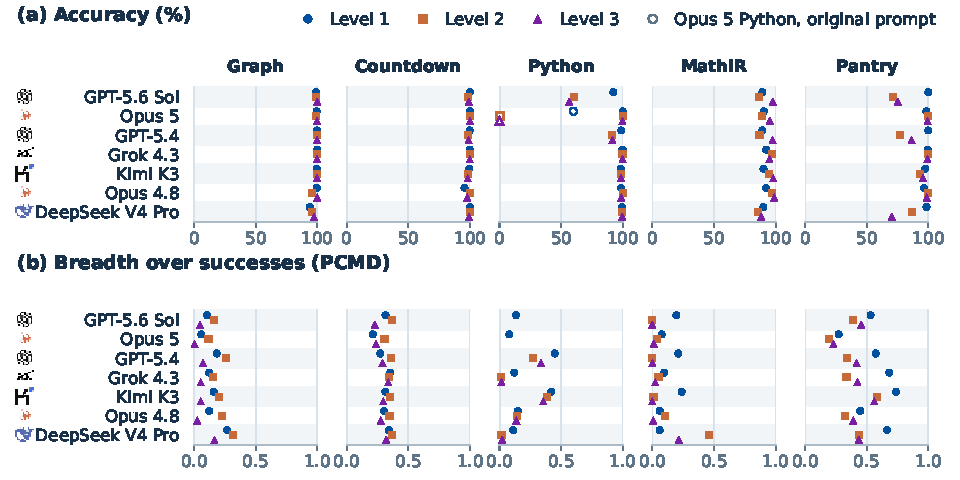
\includegraphics[width=\linewidth]{figures/hosted_verified_breadth.pdf}
  \caption{\textbf{Accurate hosted responses can still concentrate on few solution modes.}
  Columns show domains; colors and marker shapes distinguish Levels~1--3.
  Each deployment--domain--level cell uses 128 prompts and eight responses
  per prompt. Top: formatting-normalized response accuracy. Solid Opus~5
  \texttt{Python} marks use revised task wording without a system message; hollow marks
  show original wording. Bottom: promptwise \pmd{} under strict grading
  and original wording for every deployment, averaging over prompts with
  at least two verified draws. Cells with fewer than thirty eligible prompts
  are omitted. Thus the two rows use different grading and, for Opus~5
  \texttt{Python}, different prompt conditions. All marks are point estimates.
  Table~\ref{tab:hosted-level-averages-medium} gives per-level means;
  Table~\ref{tab:hosted-level-averages-parity} gives normalized success and
  mode counts on the four domains with common wording.}
  \label{fig:hosted-verified-breadth}
\end{figure}

% Generated by ops/build_paper_hosted_level_averages.py; do not edit.
\paragraph{Evaluation parity across deployments.}
One column of this cohort rests on wording the other deployments did not
answer: Claude Opus 5's Python cells in Fig.~\ref{fig:hosted-verified-breadth}
and Table~\ref{tab:hosted-level-averages-medium} use the revised condition of
App.~\ref{app:hosted-python-prompt}. Every other reading in this paper holds one
prompt across all seven deployments, including the \pmd{} column beside them,
Table~\ref{tab:hosted-cohort-mode-diversity} and the strict and normalized cell
tables above. Table~\ref{tab:hosted-level-averages-parity} therefore repeats the
comparison over Graph, Countdown, MathIR and Pantry alone, the four domains that share
one prompt. Claude Opus 5 averages
1.42/1.45/1.35 verified modes there at Levels 1--3,
against 1.43/1.44/1.36 over five domains with the
revised Python cell and 1.36/1.17/1.08
with the original one. It is the least varied deployment at every level under all
three readings, and the revised wording raises its Python breadth rather than
lowering it, so the substituted cell moves the five-domain reading away from
concentration rather than towards it. Which of the other six follows it varies
with Python in or out, as their per-domain disagreement in
Table~\ref{tab:hosted-cohort-mode-diversity} already reports; what survives every
reading is the level, not the order.
How far a Python wording change can carry this domain is itself measured, on
three of the other six: App.~\ref{app:sampling-budget-effects}
answers Python under two wordings at 16 prompts and
64 draws, and pooled \pmd{} moves by between
+.024 and +.131 across its
six deployment--level cells, leaving every one of them concentrated
under both wordings (highest \pmd{} .369,
$\neff$ 1.58). That bounds how far wording carries
this domain; it does not identify what this particular revision would do to a
deployment other than the one that answered it.

\begin{table}[H]
  \centering
  \small
  \setlength{\tabcolsep}{5pt}
  \begin{tabular}{lrrrrrr}
    \toprule
    & \multicolumn{2}{c}{Level 1} & \multicolumn{2}{c}{Level 2} & \multicolumn{2}{c}{Level 3} \\
    \cmidrule(lr){2-3}\cmidrule(lr){4-5}\cmidrule(lr){6-7}
    Model & \texttt{pass@8} (\%) & \# modes & \texttt{pass@8} (\%) & \# modes & \texttt{pass@8} (\%) & \# modes \\
    \midrule
    GPT-5.6 Sol & 97.5 & 1.90 & 98.2 & 1.59 & 99.4 & 1.54 \\
    Claude Opus 5 & 97.9 & 1.42 & 99.6 & 1.45 & 99.8 & 1.35 \\
    GPT-5.4 & 97.7 & 2.00 & 98.0 & 1.68 & 99.4 & 1.62 \\
    Grok 4.3 & 99.4 & 2.12 & 100.0 & 1.70 & 100.0 & 1.68 \\
    Kimi K3 & 98.0 & 2.26 & 100.0 & 1.95 & 100.0 & 1.79 \\
    Claude Opus 4.8 & 98.4 & 1.70 & 100.0 & 1.75 & 99.8 & 1.56 \\
    DeepSeek V4 Pro & 98.0 & 2.16 & 98.8 & 2.04 & 99.6 & 1.75 \\
    \bottomrule
  \end{tabular}
  \caption{\textbf{Hosted success and output diversity with Python excluded.}
  The same draws as Table~\ref{tab:hosted-level-averages-medium}, averaged over
  Graph, Countdown, MathIR and Pantry alone: the four domains every deployment answers
  under one prompt, 128 prompts each and eight responses per prompt. Reading this
  table beside that one shows what the revised Python condition of
  App.~\ref{app:hosted-python-prompt} carries, and what it does not.}
  \label{tab:hosted-level-averages-parity}
\end{table}


% Generated by ops/build_paper_gpt56sol_python_parity.py; do not edit.
\subsection{The revised \texttt{Python} wording on a second deployment}
\label{app:python-wording-second-deployment}

The original and revised \texttt{Python} conditions of App.~\ref{app:hosted-python-prompt}
are evaluated on GPT-5.6 Sol through \path{api.openai.com}. Each condition uses
the same 384 problems, with 128 prompts per level and eight responses per prompt,
medium reasoning effort and an 8,192-token output cap. The original condition
uses the benchmark request; the revised condition asks for a direct expression
without a system message. Public task inputs, allowed operators and the verifier
are unchanged, but wording and system-message presence change together.
Every response reports the model \texttt{gpt-5.6-sol}, but this build cannot be
shown to match the Azure deployment used for the hosted averages, so the two
are treated as separate populations.

\paragraph{Verified success and mode counts decrease under the revised condition.}
There are no provider-declared refusals among the
6,144 responses in this comparison.
The Azure GPT-5.6 Sol cohort also contains no provider-declared refusals;
its missing strict \texttt{Python} diversity entries reflect too few verified draws.
Under normalized grading, the revised condition lowers accuracy and mean
\texttt{distinct@8} at each level (Table~\ref{tab:gpt56sol-python-parity}).
Revised-minus-original differences use all 128 prompts per level, pairing
problems across conditions and resampling whole eight-response groups:
20,000 replicates give pointwise 95\% percentile intervals.
Accuracy differences are fractions of responses; mode-count differences are
modes per prompt:
accuracy $-.689$ $[-.745, -.631]$, $-.420$ $[-.467, -.374]$, $-.370$ $[-.418, -.320]$ at Levels 1--3;
\texttt{distinct@8} $-.945$ $[-1.078, -.820]$, $-.703$ $[-.812, -.594]$, $-.656$ $[-.766, -.547]$ respectively.
The revised normalized cells have
28, 26, 25
prompts with at least two verified responses, all below the 30-prompt
reporting threshold, so their success-conditional diversity and any diversity
contrast are omitted.

\paragraph{Formatting failures accompany the lower scores.}
The literal \LaTeX{} marker \verb|\text{| appears in
862 original-condition and
2,089 revised-condition responses
(28\% and 68\%).
The formatting normalizer does not remove this wrapper; none of these responses
verifies. Among responses without the marker, normalized success is
94.9\% and 59.3\%, respectively.
Absence of this marker does not guarantee parseability. Because the marker
depends on the response, these subsets are not matched comparisons and do not
bound a content or capability effect.

\paragraph{Prompt-interface sensitivity differs across deployments.}
The revised condition increases normalized success and verified mode counts
for Opus 5 (App.~\ref{app:hosted-python-prompt}) but decreases both for this
GPT-5.6 Sol deployment. This comparison does not isolate task wording from the
system message, establish that either task is generally easier, or identify
the effect on the remaining hosted deployments. The four-domain comparison in
Table~\ref{tab:hosted-level-averages-parity} holds the task prompts fixed across
all seven deployments by excluding \texttt{Python}.

\begin{table}[!htbp]
  \centering
  \caption{\textbf{The revised \texttt{Python} condition lowers normalized success and verified mode counts on GPT-5.6 Sol.}
  Both conditions use the same 128 problems per level and eight responses per
  prompt through \texttt{api.openai.com}, with medium reasoning effort and an
  8,192-token output cap. R counts provider-declared refusals; A is response
  accuracy (\%); D is mean \texttt{distinct@8} over all prompts.
  $1-C$ is pair-pooled diversity: the fraction of correct pairs with different
  solution modes, weighting each correct pair equally across prompts.
  Dashes mark cells with fewer than 30 prompts containing at least two
  verified draws. Strict grading uses the original output; normalized grading
  applies the same typography rules to both conditions. Entries are point
  estimates; paired uncertainty for accuracy and mode-count differences is
  given in the surrounding text.}
  \small
  \setlength{\tabcolsep}{4pt}
  \begin{tabular}{@{}llrrrrrrr@{}}
    \toprule
    & & & \multicolumn{3}{c}{Strict} & \multicolumn{3}{c}{Normalized} \\
    \cmidrule(lr){4-6}\cmidrule(lr){7-9}
    Wording & L & R & A & D & $1-C$ & A & D & $1-C$ \\
    \midrule
    Original & 1 & 0 & 37.0 & 1.02 & .106 & 89.8 & 1.36 & .114 \\
     & 2 & 0 & 10.4 & 0.14 & --- & 58.7 & 1.15 & .053 \\
     & 3 & 0 & 13.0 & 0.16 & --- & 56.3 & 1.13 & .048 \\
    \midrule
    Revised, no system & 1 & 0 & 18.7 & 0.27 & --- & 20.9 & 0.41 & --- \\
     & 2 & 0 & 13.4 & 0.26 & --- & 16.7 & 0.45 & --- \\
     & 3 & 0 & 15.5 & 0.25 & --- & 19.3 & 0.48 & --- \\
    \bottomrule
  \end{tabular}
  \label{tab:gpt56sol-python-parity}
\end{table}


% Generated by ops/build_paper_hosted_reasoning_off.py; do not edit.
\begin{table}[H]
  \centering
  \small
  \setlength{\tabcolsep}{5pt}
  \begin{tabular}{lrrrrrr}
    \toprule
    & \multicolumn{2}{c}{Level 1} & \multicolumn{2}{c}{Level 2} & \multicolumn{2}{c}{Level 3} \\
    \cmidrule(lr){2-3}\cmidrule(lr){4-5}\cmidrule(lr){6-7}
    Model & \texttt{pass@8} (\%) & \# modes & \texttt{pass@8} (\%) & \# modes & \texttt{pass@8} (\%) & \# modes \\
    \midrule
    \raisebox{-0.15em}{
\includegraphics[width=1.05em,height=1.05em,keepaspectratio]{icons/openai.png}}\hspace{0.4em}GPT-5.6 Sol & 82.5 & 1.31 & 66.9 & 0.76 & 76.2 & 0.88 \\
    \raisebox{-0.15em}{
\includegraphics[width=1.05em,height=1.05em,keepaspectratio]{icons/openai.png}}\hspace{0.4em}GPT-5.4 & 82.5 & 1.67 & 71.2 & 0.92 & 70.0 & 0.94 \\
    \raisebox{-0.15em}{
\includegraphics[width=1.05em,height=1.05em,keepaspectratio]{icons/grok_official_docs_print.png}}\hspace{0.4em}Grok 4.3 & 82.5 & 1.64 & 86.9 & 1.41 & 90.0 & 1.45 \\
    \raisebox{-0.15em}{
\includegraphics[width=1.05em,height=1.05em,keepaspectratio]{icons/kimi.png}}\hspace{0.4em}Kimi K3 & 92.5 & 1.91 & 92.5 & 1.37 & 95.6 & 1.59 \\
    \raisebox{-0.15em}{
\includegraphics[width=1.05em,height=1.05em,keepaspectratio]{icons/claude.png}}\hspace{0.4em}Claude Opus 4.8 & 91.2 & 1.46 & 100.0 & 1.62 & 100.0 & 1.51 \\
    \bottomrule
  \end{tabular}
  \caption{\textbf{Hosted success and output diversity with reasoning disabled.}
  Each level averages five domains equally: 32 prompts per domain and eight
  responses per prompt. \texttt{pass@8} is the fraction with any verified
  response; \# modes is mean \texttt{distinct@8}, including failures.
  The frozen formatting normalizer applies throughout. Appendix~\ref{app:hosted-reasoning-control}
  gives matched medium-reasoning results.}
  \label{tab:hosted-level-averages}
\end{table}


% Generated by ops/build_paper_hosted_reasoning_off.py; do not edit.
\subsection{Matched reasoning-control comparison}
\label{app:hosted-reasoning-control}
We selected original row indices 0--31 in each of five domains and three
levels, without consulting outputs. Each model and condition therefore has
480 prompts and 3,840 responses. The medium baseline reuses the original
audited responses for these exact prompts and eight sample slots; no new
medium responses were collected. Both conditions preserve the original
system and user prompt bytes, including the original Python wording.
The 128-prompt medium results in Table~\ref{tab:hosted-level-averages-medium}
and Figure~\ref{fig:hosted-verified-breadth} are a separate, larger display;
the comparison below uses only the matched 32-prompt subset.

Only the provider reasoning control changes, with an 8,192-token output
budget retained in both conditions. GPT-5.6 Sol and GPT-5.4 request
\texttt{reasoning.effort=none}; Grok 4.3 and Kimi K3 request
\texttt{reasoning\_effort=none}. Claude Opus 4.8 requests
\texttt{thinking.type=disabled} while retaining
\texttt{output\_config.effort=medium}. These controls denote disabled
explicit reasoning at the endpoint, without establishing the absence of
hidden internal computation. Native response receipts are checked for
control violations. The same frozen formatting normalizer and canonical
mode grader apply to both conditions; the accompanying JSON retains strict
grades, domain-level counts, controls, and source hashes.

\begin{table}[H]
  \centering
  \small
  \setlength{\tabcolsep}{5pt}
  \begin{tabular}{llrrcrrc}
    \toprule
    & & \multicolumn{3}{c}{Medium reasoning} & \multicolumn{3}{c}{Reasoning disabled} \\
    \cmidrule(lr){3-5}\cmidrule(lr){6-8}
    Model & Level & \texttt{pass@8} (\%) & \# modes & \pmd{} & \texttt{pass@8} (\%) & \# modes & \pmd{} \\
    \midrule
    \raisebox{-0.15em}{
\includegraphics[width=1.05em,height=1.05em,keepaspectratio]{icons/openai.png}}\hspace{0.4em}GPT-5.6 Sol & 1 & 96.9 & 1.81 & .311 & 82.5 & 1.31 & .226 \\
     & 2 & 98.8 & 1.54 & .117 & 66.9 & 0.76 & .063 \\
     & 3 & 98.8 & 1.51 & .195 & 76.2 & 0.88 & .095 \\
    \cmidrule(l){2-8}
     & \textit{All} & 98.1 & 1.62 & .226 & 75.2 & 0.99 & .145 \\
    \addlinespace
    \raisebox{-0.15em}{
\includegraphics[width=1.05em,height=1.05em,keepaspectratio]{icons/openai.png}}\hspace{0.4em}GPT-5.4 & 1 & 96.9 & 2.06 & .338 & 82.5 & 1.67 & .347 \\
     & 2 & 99.4 & 1.68 & .162 & 71.2 & 0.92 & .134 \\
     & 3 & 99.4 & 1.82 & .247 & 70.0 & 0.94 & .160 \\
    \cmidrule(l){2-8}
     & \textit{All} & 98.5 & 1.85 & .255 & 74.6 & 1.18 & .224 \\
    \addlinespace
    \raisebox{-0.15em}{
\includegraphics[width=1.05em,height=1.05em,keepaspectratio]{icons/grok_official_docs_print.png}}\hspace{0.4em}Grok 4.3 & 1 & 100.0 & 1.93 & .211 & 82.5 & 1.64 & .493 \\
     & 2 & 100.0 & 1.62 & .136 & 86.9 & 1.41 & .296 \\
     & 3 & 100.0 & 1.54 & .121 & 90.0 & 1.45 & .314 \\
    \cmidrule(l){2-8}
     & \textit{All} & 100.0 & 1.70 & .154 & 86.5 & 1.50 & .364 \\
    \addlinespace
    \raisebox{-0.15em}{
\includegraphics[width=1.05em,height=1.05em,keepaspectratio]{icons/kimi.png}}\hspace{0.4em}Kimi K3 & 1 & 96.9 & 2.27 & .343 & 92.5 & 1.91 & .595 \\
     & 2 & 100.0 & 2.02 & .277 & 92.5 & 1.37 & .335 \\
     & 3 & 100.0 & 1.89 & .264 & 95.6 & 1.59 & .361 \\
    \cmidrule(l){2-8}
     & \textit{All} & 99.0 & 2.06 & .293 & 93.5 & 1.62 & .426 \\
    \addlinespace
    \raisebox{-0.15em}{
\includegraphics[width=1.05em,height=1.05em,keepaspectratio]{icons/claude.png}}\hspace{0.4em}Claude Opus 4.8 & 1 & 98.1 & 1.61 & .202 & 91.2 & 1.46 & .216 \\
     & 2 & 100.0 & 1.67 & .218 & 100.0 & 1.62 & .226 \\
     & 3 & 100.0 & 1.57 & .185 & 100.0 & 1.51 & .185 \\
    \cmidrule(l){2-8}
     & \textit{All} & 99.4 & 1.62 & .202 & 97.1 & 1.53 & .209 \\
    \bottomrule
  \end{tabular}
  \caption{\textbf{Matched medium and disabled reasoning, by level.}
  Each row averages 160 prompts across five domains. All eight responses
  and zero-success prompts are retained. \# modes denotes mean
  \texttt{distinct@8}; estimates use the frozen formatting normalizer.
  \pmd{} is paired within the level: it averages over the prompts of that
  level which return two verified draws in both conditions, between
  65 and 159 of the 160 per cell, and every level cell here clears the
  thirty-prompt support bar.
  The \texttt{pass@8} and \# modes columns use all 160 prompts, so the two
  axes are read on the same draws but not on the same denominators, and the
  paired count behind every level cell is retained in the accompanying
  machine-readable record alongside the per-domain counts.
  The \textit{All} row averages the same 480 prompts and 3,840 responses
  per condition with equal weight on every domain and level; its \pmd{}
  is the paired reading over the
  245--458 prompts per deployment that return two verified draws in both conditions.
  That column separates concentration from lost accuracy, since a prompt
  one condition stopped answering twice leaves the estimate rather than
  entering it as a smaller number; the per-domain readings behind it are
  retained in the accompanying JSON, together with the prompts that only
  one of the two conditions answers twice and so enter neither average.}
  \label{tab:hosted-reasoning-matched-levels}
\end{table}

\paragraph{Incomplete deployments.}
Five of seven registered deployments passed complete-cohort admission,
and neither partial cohort receives a score. They fall short in different
ways, and that decides what can still be read from each.

DeepSeek V4 Pro's draws are intact, so its measurement survives its
exclusion and is reported here: read on the 437 prompts both of its
conditions define, disabling reasoning moves \pmd{} from
$.282$ to $.369$, a change of $+.087$. What that figure
cannot do is join the table, for two reasons and neither is the recovery
shortfall: both of its arms are graded strictly, because the frozen
normalizer was only ever run on admitted cohorts, and one PantryPlan prompt
holds seven draws rather than eight. A caveat cannot put a strictly graded
number on the same scale as a normalized one. The shortfall itself is
slight --- 3,839 of 3,840 sample receipts were recovered, leaving one
unresolved request, which is not counted as a failure --- and it is not
what keeps the deployment out of the table. The figure is reported so the
evidence is not lost, not so it can be compared.

Claude Opus 5 admits no such reading. A native response returned a thinking
block and 40 thinking tokens despite an explicit disabled-thinking request,
so its disabled condition did not disable reasoning. There is no
reasoning-off measurement to preserve, rather than one withheld.

\paragraph{Scope of the comparison.}
Across all five complete deployments, disabling reasoning lowers both
overall \texttt{pass@8} and observed \distk{}. Reduced success also
reduces opportunities to observe distinct successful modes, so those two
columns cannot separate concentration from lost accuracy. \pmd{} can, and
the answer is not uniform: on the prompts both conditions define, breadth
falls for GPT-5.6 Sol and GPT-5.4, is unchanged for Claude Opus 4.8, and
rises for Kimi K3 and Grok 4.3, which more than doubles from $.154$ to
$.364$ while its \distk{} falls. Disabling deliberation concentrates some
deployments and spreads others, so the common fall in \distk{} tracks the
accuracy drop rather than a shared collapse.
Table~\ref{tab:hosted-reasoning-matched-levels} reads the same contrast at
each level, and the direction belongs to the deployment rather than to the
level: GPT-5.6 Sol falls at every level, Grok 4.3 and Kimi K3 rise at
every level, GPT-5.4 is flat at Level 1 and falls at Levels 2 and 3, and
Claude Opus 4.8 stays within $.014$ of zero throughout.
No deployment reverses its own direction from one level to the next, and
no level cell loses the measurement: every one clears the support bar on
prompts both conditions answer twice. Medium and disabled outputs
were collected at different times; matching sample slots are not shared
random seeds. Omitted temperature and \texttt{top\_p} controls retain
provider defaults, which can vary over time. These are descriptive point
estimates without uncertainty intervals, not causal claims about training.


\clearpage
\phantomsection
\begin{center}\large\textbf{Part VI. Idealized analysis}\end{center}
\addcontentsline{toc}{part}{Part VI. Idealized analysis}

\section{Mode Collapse and Verified Replay}
\label{app:theory}

This part collects the idealized analysis behind
Section~\ref{sec:collapse-mechanism}. The winner-take-all limit of
binary-reward policy gradient among equally rewarded outcomes is established
by \citet{sinha2026expected} and \citet{lochab2026ucpo} and is a replicator
system in the sense of \citet{hofbauer1998evolutionary}; we restate it in our
categorical model so that the later statements share its notation, and we do
not reprove it. What this part adds is: an exact identity showing that every
outcome-binary advantage induces the same conditional trajectory, so the
choice among Dr.GRPO, GRPO, and MaxRL rescales time without changing which
mode survives; a starvation bound showing that fresh groups supply no gradient
to a rare mode as its probability vanishes, whereas a fixed verified buffer
does; a uniform-in-time probability floor for every buffered mode under a
fixed replay dose, with the coupon-collection ordering that makes uniform
allocation optimal for finite-budget coverage; and the stationary target of a
reference-KL anchor, whose conditional allocation is the reference's. Every
statement is for one isolated prompt with independent categorical logits and
Euclidean expected-gradient flow. These results do not certify the
implemented AdamW/PPO trajectories. The final subsection states where the
assumptions stop and which signs and orderings the runs were checked against.
Table~\ref{tab:notation} defines the notation.

\subsection{Categorical model, and the known winner-take-all limit}
\label{app:theory-grpo-mean}
\label{app:theory-collapse}
\label{app:theory-objective-inertness}

The categorical model assigns one independent logit to each outcome
category. Its Euclidean mean flow and the subsequent finite-step, sampled,
and neural updates have different assumptions; a neural solution mode need
not have an independently optimized logit.

\begin{assumption}[Categorical mean-flow model]
\label{ass:categorical-mean-flow}
Fix one isolated prompt and a finite category set
$\mathcal A=\mathcal C\mathbin{\dot\cup}\mathcal N$ with $m\ge2$ correct
solution modes and $n\ge1$ incorrect categories, and set
$p_a=\operatorname{softmax}(z)_a$, $P=\sum_{c\in\mathcal C}p_c$, and
$q_c=p_c/P$, so that $P$ measures correctness while $q$ describes how that
correct probability is allocated among the individual correct modes.
\begin{enumerate}
\item[(A1)] \emph{Independent logits.} The policy carries one independently
  optimized logit for every category in $\mathcal A$, including one separate
  logit for each canonical correct mode.
\item[(A2)] \emph{Common length normalization.} Every response uses the same
  fixed length-normalization factor, absorbed into the positive coefficient
  of the group estimator.
\item[(A3)] \emph{Euclidean mean flow.} Updates are the infinitesimal expected
  updates in these logits, taken without optimizer preconditioning and without
  momentum carried between steps.
\item[(A4)] \emph{No competing regularizer.} Explicit reference KL is zero and
  no entropy term is present.
\item[(A5)] \emph{Nondegenerate start.} Logits are finite initially,
  $0<P(0)<1$, and the group size is $G\ge2$.
\end{enumerate}
\end{assumption}

Assumption~\ref{ass:categorical-mean-flow} comprises conditions (A1)--(A5).
AdamW's preconditioning and momentum violate (A3); finite, repeated PPO
updates are outside its infinitesimal on-policy limit. Response-specific
length normalization violates (A2), while reference KL and entropy
regularization violate (A4).

A language model induces probabilities over canonical outcomes, but those
probabilities alone do not determine its update geometry. Aggregating several
response strings into a mode does not generally commute with gradient flow
in response logits. The independent-category model therefore requires an
additional assumption beyond a neural policy and its validator equivalence
classes.

Draw a group $Z_1,\ldots,Z_G\stackrel{\mathrm{iid}}{\sim}p$ with $G\ge2$,
write $R_i=\1[Z_i\in\mathcal C]$, and let $R=\sum_iR_i$. At the on-policy
point where the PPO ratio equals one, consider the common-length estimator
\begin{equation}
  \widehat g_G
  =\frac1G\sum_{i=1}^G
   w(R)\left(R_i-\frac{R}{G}\right)\nabla_z\log p_{Z_i}.
  \label{eq:group-estimator}
\end{equation}
For the Dr.GRPO abstraction \citep{liu2025understanding}, $w(R)=1$ after
absorbing the fixed positive length-normalization factor. Reward-standardized
GRPO \citep{shao2024deepseekmath} with fixed common response-length
normalization takes $w(R)$ to be the reciprocal group reward standard
deviation on mixed groups (with a fixed numerical stabilizer if used).
Standard variable-length GRPO also weights each response by its own inverse
length; that response-specific factor cannot generally be absorbed into
$w(R)$ and is outside this equivalence.
In both cases, $0<w(\ell)<\infty$ for
$\ell\in\{1,\ldots,G-1\}$. The entire update is zero on all-equal
groups, without evaluating an undefined reciprocal standard deviation;
likewise, $w(R)R(G-R)$ below is defined as zero when $R=0$ or $R=G$. All
advantages and normalization weights are detached in the score estimator.

\begin{lemma}[A group baseline does not remove frequency amplification]
\enforcehalffinalproseline
\label{lem:grpo-mean}
For $0<P<1$, the expected update in Equation~\eqref{eq:group-estimator} is
\begin{equation}
  \E[\widehat g_G]
  =c_G(P)\nabla_z P,
  \qquad
  c_G(P)=
  \frac{\E\!\big[w(R)R(G-R)\big]}{G^2P(1-P)}>0.
  \label{eq:expected-group-gradient}
\end{equation}
For the Dr.GRPO abstraction, $c_G(P)=(G-1)/G$. Group centering and reward
standardization rescale the expected gradient without changing its direction
under these assumptions.
\end{lemma}

\begin{proof}
\enforcehalffinalproseline
Condition on the complete binary reward vector, whose sum is $R$. The score
identities give
\[
  \E[\nabla_z\log p_{Z_i}\mid R_i=1]=\nabla_z\log P,
  \qquad
  \E[\nabla_z\log p_{Z_i}\mid R_i=0]
  =\nabla_z\log(1-P).
\]
There are $R$ correct rows with centered reward $(G-R)/G$ and $G-R$
incorrect rows with centered reward $-R/G$. Therefore the conditional
expectation of the unaveraged sum in~\eqref{eq:group-estimator} is
\[
  w(R)\frac{R(G-R)}{G}
  \left(\nabla_z\log P-\nabla_z\log(1-P)\right)
  =w(R)\frac{R(G-R)}{GP(1-P)}\nabla_zP.
\]
The outer factor $1/G$ and expectation over
$R\sim\operatorname{Binomial}(G,P)$ yield~\eqref{eq:expected-group-gradient}.
For $w\equiv1$,
$\E[R(G-R)]=G(G-1)P(1-P)$, proving the Dr.GRPO value.
\end{proof}

The binomial identity also gives the denominator-free expression
\[
 c_G(P)=\frac{G-1}{G}\sum_{j=0}^{G-2}\binom{G-2}{j}
 w(j+1)P^j(1-P)^{G-2-j}.
\]
The binomial weights sum to one, so $c_G$ lies between
$(G-1)\min_j w(j+1)/G$ and $(G-1)\max_j w(j+1)/G$.
Thus $c_G$ extends smoothly and positively to $P=0,1$.

The practical MaxRL estimator has the same mean-gradient direction
\citep[Section~4.3 and App.~D, Theorem~5]{tajwar2026maxrl}. Its all-failure
convention determines the finite-group coefficient.

\begin{lemma}[Binary MaxRL has the same correctness-gradient direction]
\enforcehalffinalproseline
\label{lem:maxrl-mean}
Under Assumption~\ref{ass:categorical-mean-flow}, let MaxRL assign
$A_i^{\mathrm{MaxRL}}=GR_i/R-1$ when $R>0$ and zero when $R=0$, as in
Section~\ref{app:binary-maxrl}. For
$\widehat g_G^{\mathrm{MaxRL}}=G^{-1}\sum_i
 A_i^{\mathrm{MaxRL}}\nabla_z\log p_{Z_i}$ at the on-policy point, the
expected update is
\begin{equation}
  \E[\widehat g_G^{\mathrm{MaxRL}}]
  =c_G^{\mathrm{MaxRL}}(P)\nabla_zP,
  \qquad
  c_G^{\mathrm{MaxRL}}(P)
  =\frac{1-(1-P)^{G-1}}{P}>0,
  \label{eq:maxrl-expected-gradient}
\end{equation}
with continuous endpoint values
$c_G^{\mathrm{MaxRL}}(0)=G-1$ and
$c_G^{\mathrm{MaxRL}}(1)=1$.
\end{lemma}

\begin{proof}
\enforcehalffinalproseline
With $N=G$ and pass rate $P$, the estimator in
\citet[Theorem~5]{tajwar2026maxrl} equals
$\widehat g_G^{\mathrm{MaxRL}}$. Its expected coefficient is
$\sum_{j=0}^{G-2}(1-P)^j$, whose geometric sum gives
Equation~\eqref{eq:maxrl-expected-gradient} and its endpoint values.
The identity requires on-policy independent draws and the score identity.
\end{proof}

Integrating this coefficient gives the potential
\begin{equation}
 \Psi_{\mathrm{MaxRL}}(P)
 :=\int_0^P c_G^{\mathrm{MaxRL}}(s)\,ds
 =\sum_{k=1}^{G-1}\frac{1-(1-P)^k}{k}.
 \label{eq:maxrl-potential-finite-sum}
\end{equation}
In particular, $\Psi_{\mathrm{MaxRL}}(1)=\sum_{k=1}^{G-1}1/k$.
For binary rewards, best@\(k\) equals pass@\(k\), so this is a harmonic
mixture of sampling objectives for $k=1,\ldots,G-1$. The upper limit is
$G-1$ because the implemented centered estimator sets the entire update
to zero on all-failure groups. Subtracting an unconditional score baseline
even on those groups instead gives the order-$G$ estimator. These are exact
finite-group expectations at the on-policy point; subsequent clipping and
adaptive optimization can alter the expected update.

\paragraph{Winner-take-all collapse.}
Consider $\dot z=c_G(P)\nabla_zP$, with any of the smooth positive
coefficients established above: Dr.GRPO, common-length reward-standardized
GRPO, or the specified centered binary MaxRL estimator. This infinitesimal
expected-update model has
no sampling noise and uses independently optimized Euclidean logits. The
conditional dynamics follow the frequency-dependent replicator system
with fitness $f_c(q)=q_c$
\citep{hofbauer1998evolutionary,harper2009informationgeometry}.
The limit below is the outcome-level collapse of
\citet[Theorem~3.1]{sinha2026expected} for softmax outcome logits, and the
indifference-plus-amplification mechanism of
\citet[Sections~4.1--4.2]{lochab2026ucpo}. We restate it in the present
notation and give only the reduction to the replicator flow, which is the
step the replay results reuse; it is not a new result.

\begin{proposition}[Winner-take-all collapse in the categorical mean flow]
\enforcehalffinalproseline
\label{thm:grpo-collapse}
Under Assumption~\ref{ass:categorical-mean-flow}, if the conditional correct-mode
distribution $q(0)$ has a unique largest coordinate $c^\star$, then
\[
  P(t)\longrightarrow1,
  \qquad
  q_{c^\star}(t)\longrightarrow1,
  \qquad
  q_c(t)\longrightarrow0\quad(c\ne c^\star).
\]
Thus these categorical mean flows converge to a single correct solution
mode for generic initial conditions, even though every mode in $\mathcal C$
has exactly the same reward.
\end{proposition}

\begin{proof}
\enforcehalffinalproseline
Since $\dot P=c_G(P)\lVert\nabla_zP\rVert_2^2$ with
$\lVert\nabla_zP\rVert_2^2\ge P^2(1-P)^2(1/m+1/n)$ and $c_G$ positive and
continuous on $[0,1]$, $P$ cannot converge to an interior value, so
$P\to1$. Define the effective time
$\tau(t)=\int_0^t c_G(P(s))P(s)(1-P(s))\,ds$. Every logit has absolute
velocity at most $\dot\tau$, so $\tau(\infty)<\infty$ would give every logit
finite total variation and a finite limit, contradicting $P\to1$; hence
$\tau\to\infty$. On the correct simplex the change of time gives
\begin{equation}
  \frac{dq_c}{d\tau}
  =q_c\left(q_c-\sum_{d\in\mathcal C}q_d^2\right),
  \qquad
  \frac{d}{d\tau}\log\frac{q_c}{q_d}=q_c-q_d,
  \label{eq:grpo-replicator}
\end{equation}
the replicator flow with fitness $f_c(q)=q_c$
\citep{hofbauer1998evolutionary}, which is the log-ratio dynamics of
\citet[Theorem~3.1]{sinha2026expected}. For $c\ne c^\star$ the ratio
$\xi_c=q_c/q_{c^\star}$ satisfies
$d\log\xi_c/d\tau=-q_{c^\star}(1-\xi_c)\le-(1-\xi_c(0))/m$, so every
competitor vanishes relative to the initial leader over infinite effective
time, and normalization gives $q_{c^\star}\to1$.
\end{proof}

If several modes tie for the largest initial probability, symmetry preserves
the tie; the same ratio argument eliminates strictly smaller coordinates and
leaves the tied maxima uniform. An exactly uniform correct distribution is
therefore a special initial condition. The theorem concerns limiting
concentration: finite softmax logits already give positive probabilities at
every finite time, so finite-time positivity alone is not a retention result.

\begin{remark}
Proposition~\ref{thm:grpo-collapse} is asymptotic and requires (A1)--(A5).
Finite-time support loss and convergence of the stochastic neural optimizers
used in the experiments are outside its scope.
\end{remark}

\paragraph{Every outcome-binary advantage follows the same conditional trajectory.}
Expected binary reward is the total correct mass and is indifferent to its
allocation among correct modes \citep[Section~4.1]{lochab2026ucpo}. The
following identity is the finite-group form used below: the choice among
Dr.GRPO, reward-standardized GRPO, a leave-one-out baseline, and centered
MaxRL rescales optimization time along the correctness axis without changing
the trajectory of $q$ or the identity of the surviving mode.

\begin{lemma}[Conditional inertness of outcome-binary objectives]
\label{thm:objective-inertness}
Under Assumption~\ref{ass:categorical-mean-flow}, let $a(\cdot,\cdot)$ be any
detached advantage measurable with respect to the group's binary reward
vector, applied as
$\widehat g_a=G^{-1}\sum_{i}a(R_i,R)\nabla_z\log p_{Z_i}$ at the on-policy
point. Then
\begin{equation}
  \E[\widehat g_a]=c_a(P)\,\nabla_zP,
  \qquad
  c_a(P)=\frac1G\left(
  \frac{\E[R\,a(1,R)]}{P}-\frac{\E[(G-R)\,a(0,R)]}{1-P}\right).
  \label{eq:objective-inertness}
\end{equation}
If $c_a>0$ on $(0,1)$, then under the time change
$d\tau=c_a(P)P(1-P)\,dt$ the conditional distribution $q$ obeys
Equation~\eqref{eq:grpo-replicator} exactly, for every such $a$. Dr.GRPO,
reward-standardized GRPO, a leave-one-out baseline, the centered binary MaxRL
estimator, and any reweighting shaped by a pass@$k$ target are points in this
class. The choice among them rescales optimization time along the correctness
axis and leaves both the trajectory in $q$ and the identity of the surviving
mode unchanged.
\end{lemma}

\begin{proof}
\enforcehalffinalproseline
The score identities used in Lemma~\ref{lem:grpo-mean} give
$\E[\nabla_z\log p_{Z_i}\mid R_i=1]=\nabla_z\log P$ and
$\E[\nabla_z\log p_{Z_i}\mid R_i=0]=\nabla_z\log(1-P)$.
Independence of the draws means that conditioning also on the other rows'
rewards does not change either conditional mean. Since $a(R_i,R)$ depends
only on the binary rewards, conditioning on their complete vector and
summing the $R$ successful and $G-R$ failed rows gives
\[
  \E[\widehat g_a]
  =\frac1G\Big(\E[R\,a(1,R)]\nabla_z\log P
   +\E[(G-R)\,a(0,R)]\nabla_z\log(1-P)\Big).
\]
Substituting $\nabla_z\log P=\nabla_zP/P$ and
$\nabla_z\log(1-P)=-\nabla_zP/(1-P)$ yields
Equation~\eqref{eq:objective-inertness}. Hence
$\frac{d}{dt}\log(q_c/q_d)=\dot z_c-\dot z_d=c_a(P)P(1-P)(q_c-q_d)$.
For $c_a>0$, the positive time change $d\tau=c_a(P)P(1-P)\,dt$ gives
the replicator dynamics in Equation~\eqref{eq:grpo-replicator}.
\end{proof}

For a fixed reward-dependent advantage, the binomial identities
$R\binom GR=G\binom{G-1}{R-1}$ and
$(G-R)\binom GR=G\binom{G-1}{R}$ give
\begin{equation}
 c_a(P)=\sum_{j=0}^{G-1}\binom{G-1}{j}P^j(1-P)^{G-1-j}
 \big[a(1,j+1)-a(0,j)\big],
 \label{eq:inertness-polynomial}
\end{equation}
a polynomial in $P$ of degree at most $G-1$. Finite advantage values
therefore give a smooth, bounded coefficient on $[0,1]$. This bounded coefficient is what the retention argument in
App.~\ref{app:theory-replay} uses.

\begin{corollary}[MaxRL amplification of the correctness gradient]
\enforcehalffinalproseline
\label{cor:maxrl-starvation}
For the coefficients of Lemmas~\ref{lem:grpo-mean} and~\ref{lem:maxrl-mean},
\[
 \frac{c_G^{\mathrm{MaxRL}}(P)}{c_G^{\mathrm{Dr.GRPO}}}
 =\frac{G\big[1-(1-P)^{G-1}\big]}{(G-1)P}.
\]
This ratio is nonincreasing in $P$, with limits $G$ as $P\to0$ and
$G/(G-1)$ as $P\to1$. It is strictly decreasing for $G>2$ and constant
at $2$ for $G=2$. At the same policy, MaxRL therefore multiplies the
Dr.GRPO correctness-gradient coefficient by a factor approaching $G$ when
correctness is small. The probability of a nonzero fresh task component
remains bounded by the mixed-group probability in
Lemma~\ref{lem:replay-gradient-availability} for both estimators.
\end{corollary}

\begin{proof}
\enforcehalffinalproseline
Divide $c_G^{\mathrm{MaxRL}}(P)=[1-(1-P)^{G-1}]/P$ by $(G-1)/G$.
The finite-series identity
$c_G^{\mathrm{MaxRL}}(P)=\sum_{j=0}^{G-2}(1-P)^j$
gives the endpoint limits and monotonicity. For $G=2$ the sum is the
constant $1$; for $G>2$ it contains the strictly decreasing term $1-P$.
\end{proof}

\subsection{A replay signal when fresh groups supply none}
\label{app:theory-gradient-availability}

\begin{lemma}[Fresh-group starvation]
\enforcehalffinalproseline
\label{lem:replay-gradient-availability}
Under Assumption~\ref{ass:categorical-mean-flow} with correctness probability
$P$, draw $G$ fresh categories independently. The probability of a
mixed-reward group is
\[
 h_G(P)=1-P^G-(1-P)^G\le G\min\{P,1-P\}.
\]
Every all-equal group has zero fresh task component for
Equation~\eqref{eq:group-estimator} and for the specified centered MaxRL
estimator, so the probability of a nonzero fresh task component is at most $h_G(P)$.
\end{lemma}

\begin{proof}
\enforcehalffinalproseline
The all-correct and all-incorrect events are disjoint and have probabilities
$P^G$ and $(1-P)^G$. A mixed group needs at least one correct and at least
one incorrect sample, so a union bound over the $G$ draws gives both
$h_G(P)\le GP$ and $h_G(P)\le G(1-P)$, and hence the stated minimum.
\end{proof}

\begin{lemma}[Replay ascent persists as fresh signal vanishes]
\enforcehalffinalproseline
\label{lem:replay-ascent}
Under Assumption~\ref{ass:categorical-mean-flow}, let
$\mathcal B\subseteq\mathcal C$ be a nonempty fixed verified buffer with
normalized positive weights $w_b$, let $R_w=-\sum_b w_b\log p_b$ with replay
coefficient $\rho_w>0$, and extend $w$ by zero outside the buffer to obtain $\bar w$. The
deterministic replay ascent vector is
\[
 v^{\rm replay}=-\rho_w\nabla R_w=\rho_w(\bar w-p),
\]
which vanishes only at $p=\bar w$. If $p_b\le w_b/2$ for a buffered mode, then
$v^{\rm replay}_b\ge\rho_w w_b/2$, even when $b$ is absent from the fresh
group. For a uniform buffer of $k\ge2$ modes and fixed $\rho_w>0$, as
$p\to\mathbf e_b$ at one buffered correct mode, $h_G(P)\to0$ whereas
$\|v^{\rm replay}\|_2\to\rho_w\sqrt{1-1/k}>0$.
\end{lemma}

\begin{proof}
\enforcehalffinalproseline
For $R_w=-\sum_b w_b\log p_b$, the softmax score identity gives
$\partial R_w/\partial z_a=p_a-\bar w_a$, proving the replay formula and
coordinate bound. Finally,
\[
 \|\bar w-\mathbf e_b\|_2^2=(1-1/k)^2+(k-1)/k^2=1-1/k,
\]
which gives the strictly positive limiting norm for $k\ge2$.
\end{proof}

\begin{remark}
A fixed verified buffer can supply a replay signal when the fresh task
gradient is unavailable. Lemma~\ref{lem:replay-gradient-availability}
bounds the probability of a nonzero fresh task component; it does not bound
its magnitude or account for other loss terms, clipping, or momentum. The vector in
Lemma~\ref{lem:replay-ascent} averages the fixed buffer, so a stochastic
exemplar draw realizes it only in expectation, and a nonzero logit coordinate
can still be annihilated by a degenerate neural Jacobian. Replay also need not
increase the next mixed-group probability, since $h_G(P)$ is largest at
$P=1/2$.
\end{remark}

With uniformly bounded detached advantages, the expected sampled-logit
update vanishes as the category probability tends to zero, even when
advantages depend on the group. Exact entropy gradients have unbounded
surprisal weights and therefore require a separate boundary analysis.

\begin{lemma}[Bounded sampled scores have no probability-independent boundary force]
\enforcehalffinalproseline
\label{lem:sampled-score-bound}
Under Assumption~\ref{ass:categorical-mean-flow}, condition on the training history, draw
$Z_1,\ldots,Z_G$ independently from $p$, and let $a_i$ be any detached,
possibly group-dependent advantages with $|a_i|\le B$. To interpret the
bound uniformly as $p_b\to0$, assume a finite $B$ independent of that limit.
At the on-policy point define
\[
 \widehat g=\frac1G\sum_{i=1}^G a_i(\mathbf e_{Z_i}-p).
\]
For every category $b$,
\[
 |\E[\widehat g_b]|\le\E|\widehat g_b|
 \le 2B p_b(1-p_b).
\]
On a group with no draw of $b$, exactly
$\widehat g_b=-p_bG^{-1}\sum_i a_i$; it is zero if the applied advantages
sum to zero. By comparison, the verified-replay component for a fixed target
$w$ has logit velocity $\rho(w_b-p_b)$, which approaches $\rho w_b>0$
for a buffered category as $p_b\to0$.
\end{lemma}

\begin{proof}
\enforcehalffinalproseline
Use the triangle inequality and $|a_i|\le B$. Each marginal draw satisfies
$\E|\1\{Z_i=b\}-p_b|=2p_b(1-p_b)$, irrespective of the dependence of
$a_i$ on the group. On the absence event all indicator terms are zero.
The replay formula follows by differentiating $-\sum_b w_b\log p_b$.
\end{proof}

The bound compares the isolated logit-gradient components. It does not prove
inevitable collapse, rule out retention by a bounded estimator, or guarantee
that replay dominates the full update. An unsampled mode can still change
through softmax normalization or shared parameters. Exact entropy is outside
the uniformly bounded-score premise because its surprisal is unbounded near
zero; the lemma is not an impossibility result for entropy regularization.
Nor does the absence of a mode from a finite sample establish zero probability.

\subsection{Fixed-buffer replay and retention}
\label{app:theory-replay}

Let $\mathcal B\subseteq\mathcal C$ be a nonempty fixed buffer of $k$ modes that
the policy has produced and the validator has accepted. Uniform verified replay
uses one exemplar per buffered mode and, in the categorical reduction, minimizes
\begin{equation}
  R_{\mathcal B}(z)
  =-\frac1k\sum_{b\in\mathcal B}\log p_b.
  \label{eq:verified-replay-loss}
\end{equation}
For the uniform buffer target $w$, the likelihood-replay objective is
$R_{\mathcal B}=H(w)+\mathrm{KL}(w\|p)$
\citep[App.~D.1, v4]{li2025divergence}. The target assigns mass
$1/k$ to each buffered mode and zero elsewhere. Decreasing this loss can raise
total buffer mass as well as redistribute mass within the buffer; the buffer is
not the conditioning event for $p$.

In an averaged continuous-time model, absorb a fixed round-robin replay
frequency and loss scale into an effective dose $\rho>0$. This assumes a
fixed eligible-buffer set and constant relative weighting; it does not identify
finite alternating updates with simultaneous gradient flow. For one
isolated prompt, the categorical mean flow for any of the three fresh
binary-reward estimators with verified replay is
\begin{equation}
  \dot z
  =c_G(P)\nabla_zP-\rho\nabla_zR_{\mathcal B}(z).
  \label{eq:replay-mean-flow}
\end{equation}
Let $\Psi(P)=\int_0^P c_G(s)\,ds$. For the finite-group estimators in Lemmas~\ref{lem:grpo-mean}
and~\ref{lem:maxrl-mean}, $c_G$ has a finite positive extension to $[0,1]$;
in particular, Dr.GRPO has $c_G=(G-1)/G$ and MaxRL has
$c_G=[1-(1-P)^{G-1}]/P$. More generally, Lemma~\ref{thm:objective-inertness} and
Equation~\eqref{eq:inertness-polynomial} give
$c_a(P)\nabla_zP$ for every fixed, bounded reward-measurable advantage,
with $c_a$ a polynomial. Its integral $\Psi_a$ is also bounded on $[0,1]$,
so the retention argument applies even when the fresh coefficient changes
sign. Define
\begin{equation}
  F_{\mathcal B}(z)=\rho R_{\mathcal B}(z)-\Psi(P(z)).
  \label{eq:replay-potential}
\end{equation}
Then~\eqref{eq:replay-mean-flow} is exactly gradient flow
$\dot z=-\nabla_zF_{\mathcal B}$.

\begin{theorem}[Verified replay prevents buffered-mode extinction]
\enforcehalffinalproseline
\label{thm:replay-retention}
Under Assumption~\ref{ass:categorical-mean-flow}, suppose logits are finite
at time $T$ and thereafter the nonempty verified buffer $\mathcal B$ is fixed,
fits within replay capacity, and receives a
fixed positive effective replay dose $\rho$, the fresh objective being any
bounded reward-measurable one in the sense of
Lemma~\ref{thm:objective-inertness}. Set
$\Psi_{\max}=\max_{s\in[0,1]}\Psi(s)$, which is finite, and under
\eqref{eq:replay-mean-flow} define
\[
  C_T
  =R_{\mathcal B}(z(T))
   +\frac{\Psi_{\max}-\Psi(P(T))}{\rho}.
\]
Then for every $b\in\mathcal B$ and every $t\ge T$,
\begin{equation}
  p_b(t)\ge \exp(-kC_T)>0.
  \label{eq:replay-retention-bound}
\end{equation}
Thus each buffered probability is uniformly bounded away from zero for all
$t\ge T$, including asymptotically, even when the buffer does not cover every
correct mode. This is stronger than finite-time positivity, which already
follows from finite softmax logits without replay.
\end{theorem}

\begin{proof}
\enforcehalffinalproseline
The smooth vector field has bounded velocity because $c_G$,
$\nabla_zP$, and $\nabla_zR_{\mathcal B}$ are bounded, so finite initial
logits give a flow for every finite $t\ge T$. Along this flow,
\[
  \frac{d}{dt}F_{\mathcal B}(z(t))
  =-\lVert\nabla_zF_{\mathcal B}(z(t))\rVert_2^2\le0.
\]
Since $\Psi(P(t))\le\Psi_{\max}$,
\[
  R_{\mathcal B}(z(t))
  \le R_{\mathcal B}(z(T))
     +\frac{\Psi_{\max}-\Psi(P(T))}{\rho}
  =C_T.
\]
Every $-\log p_b$ is nonnegative and their sum is
$kR_{\mathcal B}$. Therefore
$-\log p_b(t)\le kC_T$ for every buffered mode, which is exactly
Equation~\eqref{eq:replay-retention-bound} for every time after $T$.
\end{proof}

For the nonnegative coefficients of the named fresh estimators,
$\Psi_{\max}=\Psi(1)$, recovering the simpler constant. Signed coefficients
also satisfy the retention bound, but need not yield $P\to1$.
The elementary floor is qualitative and can be numerically vacuous. For example, at
$k=16$ even a hypothetical $C_T=160$ gives $e^{-2560}$, far below any useful
evaluation probability. The argument establishes a uniform-in-time lower
bound in the stated ideal flow, not practical visibility or a prediction for
the experimental replay loss. The effective dose also depends on relative
fresh/replay frequencies, not the replay coefficient alone.

A common nonnegative, locally integrable rate $\eta(t)$ multiplying both
terms of~\eqref{eq:replay-mean-flow} preserves the energy bound, since
$\dot F_{\mathcal B}=-\eta(t)\|\nabla F_{\mathcal B}\|_2^2\le0$.
The convergence statements below additionally require
$\int_T^\infty\eta(t)\,dt=\infty$ and then follow by reparameterizing
optimization time. Infinitely many replay visits alone establish neither
this condition nor a fixed replay-to-fresh weighting. Different time-varying
relative weights are outside the fixed-potential argument.

\paragraph{Full coverage and the categorical target.}
\begin{corollary}[Conditional full-coverage categorical limit]
\enforcehalffinalproseline
\label{cor:replay-no-collapse}
Assume the conditions of Theorem~\ref{thm:replay-retention} and that by time
$T$ the buffer covers the full correct support, $\mathcal B=\mathcal C$.
Assume additionally $c_G(P)\ge0$ on $[0,1]$, as for the three named
estimators. Let
$u_c=1/m$ on $\mathcal C$. Then the categorical mean flow converges to
\[
  P(t)\longrightarrow1,
  \qquad q(t)\longrightarrow u.
\]
Consequently
\[
  \min_{c\in\mathcal C}q_c(t)\longrightarrow\frac1m,
  \qquad
  \mathcal H(q(t))\longrightarrow\log m,
\]
so asymptotic concentration onto a strict subset of the correct modes is
impossible under full coverage. \pmd{} may nevertheless decline transiently
before converging to its uniform maximum.
\end{corollary}

\begin{proof}
\enforcehalffinalproseline
For full coverage,
\begin{equation}
 R_{\mathcal C}=\log m-\log P+\mathrm{KL}(u\|q).
 \label{eq:replay-mass-uniformity-decomposition}
\end{equation}
The potential is bounded below by $-\Psi_{\max}$, so its descent gives
$\int_T^\infty\|\nabla F_{\mathcal C}\|_2^2dt<\infty$. The fixed reward-measurable
advantage gives a smooth $c_G$ on $[0,1]$, and softmax derivatives and the cross-entropy
gradient are bounded. Thus the Hessian of $F_{\mathcal C}$ and the velocity
are bounded; the gradient along the trajectory is uniformly continuous.
Square integrability then implies $\nabla F_{\mathcal C}\to0$: recurring
gradients of fixed positive size would otherwise contribute energy over
intervals of a uniform minimum length.

Every limiting probability vector therefore satisfies the correct-coordinate
equations
\[
 0=\rho(p_c-1/m)-c_G(P)p_c(1-P).
\]
Summing them gives $0=-(1-P)(\rho+c_G(P)P)$, hence $P=1$. Each correct
coordinate is then $1/m$ and every incorrect coordinate is zero. Compactness
of the probability simplex and uniqueness of this limit establish convergence
of the probability vector.
\end{proof}

\begin{corollary}[Uniform allocation maximizes finite-budget coverage]
\enforcehalffinalproseline
\label{cor:coupon-uniform-coverage}
Fix correctness $P\in(0,1]$ and $m\ge2$ possible correct keys.
Let $D_K(P,q)$ count distinct verified keys in $K$ independent draws with
key probabilities $Pq_1,\ldots,Pq_m$ and failure probability $1-P$.
For $u=(1/m,\ldots,1/m)$, every $K\ge1$ and $r=1,\ldots,m$ satisfy
\begin{equation}
 \Pr[D_K(P,u)\ge r]\ge\Pr[D_K(P,q)\ge r].
 \label{eq:coupon-uniform-coverage}
\end{equation}
Thus uniform conditional allocation maximizes expected \texttt{distinct@}$K$
at fixed correctness, as well as every coverage tail probability. This is
the coupon-collection ordering of
\citet[Theorem~3, v1]{anceaume2015coupon}, applied to independent draws
from a fixed policy over a finite catalogue of verified execution keys.
\end{corollary}
\begin{proof}
\enforcehalffinalproseline
Map each correct key to a coupon of mass $Pq_c$ and every failure to the
null coupon of mass $1-P$. The cited theorem makes the time to collect $r$
distinct non-null coupons stochastically smallest when each has mass $P/m$.
The event that this time is at most $K$ is exactly $D_K\ge r$.
Zero coordinates and $P=1$ follow by continuity of finite-horizon
probabilities. Summing the tail inequalities over $r=1,\ldots,m$ gives the
same ordering of expected distinct counts for every finite sampling budget
at the same correctness level and over the same catalogue of possible keys.
\end{proof}
This sampling optimum does not assert that a training algorithm reaches the
uniform allocation.

\paragraph{Positive weights and the implemented length normalization.}
Uniformity of the target is separate from protection against extinction.
For fixed weights $w_b>0$ with $\sum_{b\in\mathcal B}w_b=1$, define
$R_w=-\sum_b w_b\log p_b$ and use replay coefficient $\rho_w>0$.
The same potential argument gives, for all $t\ge T$,
\[
 p_b(t)\ge\exp(-C_{T,w}/w_b),\qquad
 C_{T,w}=R_w(z(T))+\frac{\Psi_{\max}-\Psi(P(T))}{\rho_w}.
\]
For the following convergence statements assume $c_G\ge0$.
If $\mathcal B=\mathcal C$, then
$R_w=H(w)-\log P+\mathrm{KL}(w\|q)$, and the independent-logit limit is
$P\to1$, $q\to w$. The preceding stationarity proof applies with $1/m$
replaced by $w_c$: summing the correct-coordinate equations forces $P=1$,
then each equation forces $p_c=w_c$.

A partial buffer has a stronger limitation in this same ideal flow. For any
fixed nonempty $\mathcal B\subseteq\mathcal C$ and fixed positive weights
summing to one, extend $w$ by zero to $\bar w$ on all categories. Then
$p(t)\to\bar w$, so even correct modes outside the fixed buffer vanish
asymptotically. For $F=\rho_wR_w-\Psi(P)$, the preceding energy and
bounded-Hessian argument still gives $\nabla F\to0$; neither argument
requires full buffer coverage.
At every subsequential probability limit, the correct-coordinate equations are
\[
 0=\rho_w(p_c-\bar w_c)-c_G(P)p_c(1-P).
\]
Summing over correct categories gives
$0=-(1-P)(\rho_w+c_G(P)P)$, hence $P=1$; each equation then gives
$p_c=\bar w_c$, and all incorrect mass is zero. Compactness and uniqueness
of this limiting probability vector prove convergence. Thus protecting a
fixed set of buffered modes need not preserve unbuffered correct alternatives.
This conclusion concerns the fixed-buffer categorical flow, not changing-buffer
or stochastic neural training.

This distinction matters for the implemented mean-token exemplar loss.
Even if each key were represented by exactly one categorical exemplar of
fixed length $L_b$, its loss would be $A R_w$, where
\[
 A=\frac1k\sum_{b\in\mathcal B}\frac1{L_b},\qquad
 w_b=\frac{L_b^{-1}}{\sum_{j\in\mathcal B}L_j^{-1}}.
\]
Its effective categorical replay coefficient would be $\rho_w=\rho A$.
The full-coverage limit would therefore weight shorter exemplars more, and
would be uniform only for equal lengths. For an actual language model,
$\pi_\theta(e_b\mid x)$ is only one contribution to the total key probability.
Equal averaging of per-token exemplar scores does not imply uniform learned
key probabilities; the categorical uniformity corollary is not that claim.

Full support is an additional premise, not a consequence of replay. In
\texttt{Python} factors, evaluation prompts admit 16--1{,}512 correct execution
modes (mean 229.44), while the buffer capacity is 16. The
full-coverage corollary therefore cannot supply a domain-wide guarantee there. The retention theorem protects only
buffered modes; it supplies no probability floor for an unbuffered key.

\subsection{Reference-KL stationary targets}
\label{app:theory-kl}

Assumption~\ref{ass:categorical-mean-flow}(A4) sets the reference-KL
coefficient to zero, as in the default training setting of
Table~\ref{tab:run-contract}. A positive fixed-reference coefficient changes
the categorical target: for Dr.GRPO and centered MaxRL, the unique
full-support stationary policy allocates its correct mass in the same
proportions as the reference, so the anchor can retain only the diversity its
reference already carries. The measured comparison is in
App.~\ref{app:kl-measured}.

For this analysis, replace (A4) by

\begin{itemize}
\item[(A4$'$)] \emph{Reference KL.} A fixed reference $\mu$ with full support
  on the category set $\mathcal A$ enters with a positive coefficient $\beta$,
  and no entropy term is present alongside it.
\end{itemize}
The KL estimator in GRPO has expectation $\mathrm{KL}(p\,\|\,\mu)$
under samples drawn from $p$ \citep{shao2024deepseekmath}. Unbiasedness of
this value does not imply that differentiating it at fixed samples gives an
unbiased gradient of the distributional KL. With the KL differentiated
exactly, write $D(z)=\mathrm{KL}(p(z)\,\|\,\mu)$. The prompt-isolated
categorical mean flow is
\begin{equation}
  \dot z=c_G(P)\nabla_zP-\beta\nabla_zD(z),
  \qquad
  \nabla_{z_b}D=p_b\big(\log(p_b/\mu_b)-D\big),
  \label{eq:kl-mean-flow}
\end{equation}
which is the negative gradient flow of
$F_\beta(z)=-\Psi(P(z))+\beta D(z)$, with $\Psi'=c_G$ as in
Equation~\eqref{eq:replay-potential}.

\begin{lemma}[Reverse-KL sublevels and replay barriers]
\enforcehalffinalproseline
\label{lem:kl-no-barrier}
For a full-support reference,
$D=\mathrm{KL}(p\|\mu)\le\log(1/\min_a\mu_a)$ on the simplex, while
$R_{\mathcal B}\to\infty$ if a buffered coordinate vanishes. More precisely,
\[
 \inf_{p:p_b=0}D(p)=\log\frac1{1-\mu_b}.
\]
Thus every finite replay-loss sublevel bounds each protected probability
away from zero. A reverse-KL sublevel $\{D\le B\}$ does so for coordinate $b$
if $B<-\log(1-\mu_b)$, but includes a point with $p_b=0$ if
$B\ge-\log(1-\mu_b)$.
\end{lemma}
\begin{proof}
\enforcehalffinalproseline
The global bound follows from $\sum_ap_a\log p_a\le0$ and
$-\sum_ap_a\log\mu_a\le\log(1/\min_a\mu_a)$.
On the face $p_b=0$, write $\widetilde\mu_a=\mu_a/(1-\mu_b)$ for $a\ne b$.
Then $D(p)=\mathrm{KL}(p\|\widetilde\mu)-\log(1-\mu_b)$, whose minimum is
attained at $\widetilde\mu$. Continuity and compactness exclude that face
from any strictly lower sublevel and give a positive coordinate minimum.
For replay, $-\log p_b\le kR_{\mathcal B}$ gives the bound directly.
\end{proof}

Descent of $F_\beta$ gives
$D(p(t))\le [F_\beta(z(T))+\Psi_{\max}]/\beta$.
This energy bound excludes the face $p_b=0$ when its right side is below
$-\log(1-\mu_b)$; an arbitrary initial energy need not satisfy that condition.
A trajectory can have a positive probability floor even when this sublevel
bound does not establish one.

\begin{proposition}[The retained conditional is the reference's]
\enforcehalffinalproseline
\label{prop:kl-stationary}
Under Assumption~\ref{ass:categorical-mean-flow} with (A4$'$), using the
Dr.GRPO or centered MaxRL coefficient, the flow
\eqref{eq:kl-mean-flow} has exactly one stationary policy of full support,
\[
  p^\star_a\propto\mu_ae^{\lambda R_a},
  \qquad
  \lambda=c_G(P^\star)/\beta,
  \qquad
  R_a=\1[a\in\mathcal C],
\]
with $\lambda=(G-1)/(G\beta)$ in closed form for the Dr.GRPO coefficient, and
a unique $\lambda$ for the MaxRL coefficient. Consequently
\[
  q^\star=\mu|_{\mathcal C},
  \qquad
  \mathcal H(q^\star)=\mathcal H(\mu|_{\mathcal C}),
  \qquad
  \operatorname{logit}P^\star=\operatorname{logit}\mu(\mathcal C)+\lambda .
\]
This stationary conditional does not depend on $\beta$: the coefficient sets
the correctness level there and leaves the allocation among correct modes at
the reference's.
\end{proposition}

\begin{proof}
\enforcehalffinalproseline
Stationarity of~\eqref{eq:kl-mean-flow} in a coordinate with $p_b>0$ reads
$c_G(P)(R_b-P)=\beta(\log(p_b/\mu_b)-D)$, so
$\log(p_b/\mu_b)=D+(c_G(P)/\beta)(R_b-P)$ and the $b$-independent terms are
absorbed by normalization, giving the stated form with $\lambda=c_G(P)/\beta$.
Conversely each $\lambda\ge0$ determines
$P(\lambda)=\mu(\mathcal C)e^\lambda/(\mu(\mathcal C)e^\lambda+1-\mu(\mathcal C))$,
strictly increasing from $\mu(\mathcal C)$ to $1$. The consistency requirement
$\lambda=c_G(P(\lambda))/\beta$ has a solution by the intermediate value
theorem, since the left side increases from $0$ without bound while the right
side is positive and bounded; it is unique whenever $c_G$ is non-increasing,
which covers the constant Dr.GRPO coefficient and
$c_G^{\mathrm{MaxRL}}(P)=[1-(1-P)^{G-1}]/P$, nonincreasing from $G-1$
to $1$ and strictly decreasing for $G>2$.
Two correct modes give $\log(p_c/\mu_c)=\log(p_d/\mu_d)$, hence
$q^\star\propto\mu$ on $\mathcal C$, which is $\beta$-free. The logit identity
is $P^\star/(1-P^\star)=[\mu(\mathcal C)/(1-\mu(\mathcal C))]e^\lambda$.
\end{proof}

Dr.GRPO with exact reference KL is an entropy-regularized softmax bandit, so
\citet[Theorem~5 and Lemma~13]{mei2020softmaxpg} give convergence of exact
gradient steps to this stationary policy together with a positive
trajectory-wide probability floor; its Gibbs target is the regularized
maximizer of \citet[Proposition~1]{geist2019regmdp}. We do not restate those
results. The contrast with replay is the one in
Lemma~\ref{lem:sampled-score-bound}: by Equation~\eqref{eq:kl-mean-flow} the
reverse-KL restoring force on a depleted coordinate is proportional to $p_b$
and vanishes with it, whereas replay's force on a buffered coordinate has the
positive limit $\rho w_b$.

\subsection{Where the categorical guarantees stop, and what was measured}
\label{app:theory-evidence-map}
\label{app:theory-entropy}
\label{app:theory-entropy-comparison}
\label{app:theory-neural-replay-response}
\label{app:theory-measured-signatures}

\paragraph{Dependence on optimization geometry.}
For a smooth parameterization $z=z(\theta)$ with Jacobian
$J_\theta=\partial z/\partial\theta$, Euclidean parameter flow instead
induces $\dot z=c_G(P)J_\theta J_\theta^\top\nabla_zP$. Proposition~\ref{thm:grpo-collapse}
uses $J_\theta J_\theta^\top=I$ and does not automatically
extend to arbitrary shared parameters or another optimization metric. Equal
binary reward alone does not force this winner selection. The natural policy
gradient update of \citet[Lemma~15]{agarwal2021policygradient}, specialized to
this bandit, is $p_a^+\propto p_a\exp(\eta c_G(P)R_a)$ and preserves
every ratio of correct probabilities at each finite step. Its continuous
version has $\dot z_a=c_G(P)(R_a-P)$, with
$R_a=\1[a\in\mathcal C]$. The distinction between Euclidean and natural
updates also underlies the tabular entropy identities of
\citet[Theorems~1--2]{cui2025entropy}; entropy and verified-mode diversity
remain different observables.

\paragraph{Exact entropy is a different comparator.}
For a known full correct support and uniform $u$, the elementary identities
\[
 H(q)=\log m-\mathrm{KL}(q\|u),\qquad
 R_u(p)=\log m-\log P+\mathrm{KL}(u\|q)
\]
show that exact conditional entropy and categorical replay both favor a
uniform conditional target. With strictly increasing correctness potential
$\Psi$, both $\Psi(P)+\beta H(q)$ and $\Psi(P)-\rho R_u(p)$ have the unique
global optimum $P=1,q=u$ in probability space on the simplex with $P>0$,
for positive coefficients. This is a boundary limit for finite-logit softmax
policies. The optimum follows from nonnegativity of KL and increasing
$\Psi$; it does not assert convergence of either neural update. The KL direction distinguishes their
loss level sets \citep{pereyra2017confidencepenalty,agarwal2021policygradient}:
replay loss diverges when a protected coordinate vanishes, whereas
conditional entropy can remain $\log(m-1)$ with one missing mode.

Exact full-output entropy is a third objective and also regularizes incorrect
mass. Exact tabular entropy-regularized policy gradient has its own positive
probability and convergence guarantees under specified assumptions
\citep{mei2020softmaxpg}; Proposition~\ref{thm:grpo-collapse} contains no entropy term.
The sampled semantic scores in the experiments are not exact gradients of
full-output or conditional verified-key entropy. Neither their empirical
comparison nor the bounded-score lemma is an impossibility result for entropy.

\paragraph{Discovery and optimization remain separate requirements.}
Retention starts after a verified key enters active memory. Actual insertion
depends on generation, validation, capacity, and eligibility; a positive
sampling probability alone does not establish eventual admission. Once a
non-evicting capacity-16 buffer fills, an unbuffered key can remain ineligible.
Changing membership or exemplar weights changes the loss being bounded, so
fixed-buffer descent cannot simply be carried across those changes. In
particular, the fixed-weight argument does not cover a target whose weights
continue to change with fresh observation counts.

Extending the fixed-potential descent to a discrete, shared-parameter
optimizer would need an energy bound of the form
$F(\theta_{n+1})\le F(\theta_n)+\epsilon_n$ with summable $\epsilon_n$, and
neither a positive replay coefficient nor a small nominal learning rate
establishes one. Adam moments, clipping, momentum, prompt scheduling, and
buffer changes are not covered by the exact-flow proofs, and the experiments
do not establish the required energy control. The one neural statement made
here is local.

With shared parameters, a replay update's effect on a particular exemplar
depends on interference among score gradients and on the optimizer's
response. A lower bound on that exemplar's change in log probability can be
obtained from the realized parameter step, without assuming any global
potential descent.

\begin{proposition}[Local replay response under shared parameters]
\enforcehalffinalproseline
\label{prop:neural-replay-local-response}
For a fixed buffer of $k$ complete exemplars, define
\[
 \ell_b(\theta)=\frac{\log\pi_\theta(e_b\mid x_b)}{L_b},\qquad
 h_b=\nabla_\theta\ell_b(\theta),\qquad
 \bar h=\frac1k\sum_{j=1}^k h_j.
\]
Suppose a step has the form
$\Delta=\eta H(g+\lambda\bar h)+u$, where $\eta,\lambda\ge0$,
$H$ is a fixed symmetric positive semidefinite matrix for this step,
$g$ is the fresh ascent direction, and $u$ is the remaining update.
Assume $\ell_b$ is twice differentiable and its Hessian has operator norm
at most $B_b$ along $\{\theta+s\Delta:0\le s\le1\}$.
Set
\[
 K_{bj}=h_b^\top Hh_j,\qquad
 \kappa_b=\frac1k\sum_jK_{bj},\qquad
 m_b=\eta h_b^\top Hg+\eta\lambda\kappa_b
       +h_b^\top u-\frac{B_b}{2}\|\Delta\|_2^2.
\]
Then
\begin{equation}
 \ell_b(\theta+\Delta)-\ell_b(\theta)\ge m_b,
 \qquad
 \pi_{\theta+\Delta}(e_b\mid x_b)
    \ge\pi_\theta(e_b\mid x_b)e^{L_bm_b}.
 \label{eq:neural-replay-local-response}
\end{equation}
In particular, $m_b>0$ guarantees that this update increases the complete
exemplar's probability, whether or not it appeared among the fresh samples.
\end{proposition}

\begin{proof}
\enforcehalffinalproseline
Taylor's theorem with the Hessian bound gives
$\ell_b(\theta+\Delta)-\ell_b(\theta)
 \ge h_b^\top\Delta-(B_b/2)\|\Delta\|_2^2$.
Substitution of the stated step and
$h_b^\top H\bar h=k^{-1}\sum_jK_{bj}$ proves the first inequality.
Multiplication by $L_b$ and exponentiation prove the second.
\end{proof}

The required replay response is a row average $\kappa_b$ of the score Gram
matrix, not only its nonnegative diagonal entry $K_{bb}$. A sufficient
interference condition is $\kappa_b>0$, with replay strength satisfying
\[
 \eta\lambda\kappa_b>
   -\eta h_b^\top Hg-h_b^\top u
       +\frac{B_b}{2}\|\Delta\|_2^2.
\]
This inequality includes the step's curvature cost, which itself depends on
the chosen dose; arbitrarily increasing $\lambda$ is not a sufficient rule.

The interference condition cannot be dropped. For example, consider three
categorical logits sharing one scalar parameter, with slopes $(1,-2,0)$.
At a point with probabilities $(s,s,1-2s)$, where $0<s<1/4$, let the first
two categories be correct and buffered. Their unit-length log-score gradients
are $h_1=1+s$ and $h_2=-2+s$. Uniform replay alone follows
$\bar h=s-1/2$, so
\[
 \left.\frac{d}{dt}\log p_1\right|_{\dot\theta=\bar h}
   =(1+s)(s-1/2)<0.
\]
Thus shared parameters can make replay initially reduce the probability of
a rare stored mode while improving the average replay score.

For an AdamW step, replay can alter both moment estimates. The proposition
therefore does not identify its $H$ with an unchanged AdamW preconditioner.
It applies to a specified decomposition of the realized step, with any
remaining contribution included in $u$; alternatively its Taylor bound can
be evaluated directly from $h_b^\top\Delta$. Neither the interference margin
nor a curvature bound is established for the experimental runs.
The statement concerns complete stored responses. Raising one such
probability strengthens that exemplar's contribution to its key, but need
not increase total key probability or transfer to a held-out prompt.

\paragraph{Assumptions and the evidence that tests them.}
The results in this part are exact for the flows they assume, and the
paragraphs above state where those assumptions stop. Each result also implies a sign,
an ordering, or a directly countable quantity that does not depend on the
exact-flow assumptions. Those implications are measured elsewhere in this
supplement. The table collects them, together with the case in which the
idealized statement does not carry over to neural training.

\begin{center}
\small
\begin{tabularx}{\linewidth}{@{}p{0.19\linewidth}Xp{0.12\linewidth}X@{}}
\toprule
\textbf{Idealized claim} & \textbf{Implication for neural training} & \textbf{Measured in} & \textbf{What the measurement shows} \\
\midrule
Lemma~\ref{lem:sampled-score-bound}: a group whose rewards agree contributes no fresh task gradient
& Under sparse binary verification many updates carry no fresh task gradient, and replay raises the fraction of mixed groups
& App.~\ref{app:degenerate-groups}
& Mixed-group fractions span $.015$--$.364$ under Dr.GRPO and $.185$--$.954$ under Re:Dr; $98.5\%$ of \texttt{Python} control updates carry zero fresh task gradient \\
\addlinespace
Proposition~\ref{thm:grpo-collapse}: winner-take-all among correct modes
& Training under binary verification retains fewer correct modes than it began with
& Fig.~\ref{fig:concentration-story}, App.~\ref{app:pre-rl-regression}
& Fewer solution modes after training in 14 of 15 comparisons; every \texttt{Python} control seed reaches byte-identical completions on all 128 prompts by steps 288--480 \\
\addlinespace
Uniform rehearsal severs rehearsal frequency from discovery frequency (Eq.~\ref{eq:lm-verified-replay})
& Rehearsing in proportion to discovery restores the self-reinforcement that uniform weighting removes, so uniform weighting retains at least as many modes
& App.~\ref{app:frequency-replay-progress}
& $+.318$ extra modes per prompt ($[+.272,+.358]$), with positive within-seed domain averages in all five seeds, driven by \texttt{Graph}, \texttt{Countdown} and \texttt{PantryPlan}; the paired $P_8$ effect $+.010$ ($[-.119,+.139]$) identifies neither a gain nor equivalence \\
\addlinespace
Theorem~\ref{thm:replay-retention} and Corollary~\ref{cor:replay-no-collapse}: a fixed buffer holds every retained mode above a positive floor
& With shared parameters the floor is not exact for an individual exemplar; typical exemplars rise while a minority falls
& App.~\ref{app:fixed-bank-survival}
& Median change $+.038$ nat/token ($[+.025,+.048]$), tenth percentile $-.256$, and $2.61\%$ of exemplars lose more than $.5$ nat/token ($[1.54,3.77]\%$) \\
\bottomrule
\end{tabularx}
\end{center}

The first three rows measure a quantity the idealized statement names, and each
carries the predicted sign. The fourth row is where the categorical guarantee
does not carry over: a per-exemplar floor is exact in the categorical flow,
while under shared parameters a measurable minority of protected exemplars
falls. Proposition~\ref{prop:neural-replay-local-response} is the statement that
applies in that setting, and it is conditional on a local response term rather
than categorical. The $P_8$ interval in the third row likewise leaves
correctness unidentified, so the ordering it supports concerns retained modes
rather than accuracy.

\paragraph{Measured signatures of the categorical predictions.}
The categorical results predict an ordering among coexisting correct modes and
a direction for which mode is lost. Both are signs rather than trajectories, so
both survive the move to AdamW, clipping and shared parameters, and both are
measurable in the runs already reported. This section measures them on the
five-domain Qwen2.5-0.5B verified-replay pairs and their matched controls
(five seeds per domain, thirty-three evaluated checkpoints per run, thirty-two
sampled draws per prompt). Canonical keys are recorded for incorrect draws as
well, so only draws carrying reward one contribute.

Two estimator choices matter. Ranking a pair of modes and measuring their
starting log-odds from the same draws biases the ordering statistic below one
half, because a mode over-sampled at a checkpoint is both more likely to be
ranked ahead and more likely to fall back at the next one; pooled over
$1.1\times10^5$ pairs that artifact alone reads $.48$ under both objectives.
The draws at each checkpoint are therefore split by index parity: one half
fixes which mode leads, the disjoint half fixes the starting log-odds, and the
next checkpoint supplies the outcome. Counts are Laplace-smoothed so that a
mode reaching zero is a defined move rather than a dropped observation;
discarding those pairs removes precisely the outcome the prediction concerns.

\begin{center}
\small
\begin{tabular}{@{}llrrrr@{}}
\toprule
& & \multicolumn{2}{c}{\textbf{Ordering}} & \multicolumn{1}{c}{\textbf{Loss}} & \textbf{Coexisting} \\
\cmidrule(lr){3-4}\cmidrule(lr){5-5}\cmidrule(lr){6-6}
\textbf{Domain} & \textbf{Arm} & pairs & $\Pr[\text{leader gains}]$ & $\Pr[\text{rarer lost}]$ & first $\to$ last \\
\midrule
\texttt{Graph} & control & 947 & $.693\ [.663,.721]$ & $.911\ [.881,.934]$ & $21.0\to0.2$ \\
               & replay  & 36{,}488 & $.551\ [.546,.557]$ & $.720\ [.711,.728]$ & $21.0\to108.2$ \\
\addlinespace
\texttt{Countdown} & control & 1{,}014 & $.546\ [.516,.577]$ & $.759\ [.720,.794]$ & $1.4\to1.0$ \\
                   & replay  & 16{,}613 & $.461\ [.454,.469]$ & $.836\ [.821,.851]$ & $1.4\to81.2$ \\
\addlinespace
\texttt{PantryPlan} & control & 6{,}081 & $.460\ [.448,.473]$ & $.719\ [.704,.734]$ & $98.2\to0.0$ \\
                    & replay  & 29{,}802 & $.522\ [.516,.528]$ & $.824\ [.816,.831]$ & $98.2\to65.0$ \\
\addlinespace
\texttt{MathIR} & control & 103 & $.447\ [.354,.543]$ & $.667\ [.516,.790]$ & $1.8\to0.2$ \\
                & replay  & 292 & $.555\ [.497,.611]$ & $.734\ [.664,.794]$ & $1.8\to5.2$ \\
\addlinespace
\texttt{Python} & replay & 718 & $.655\ [.619,.688]$ & $.938\ [.852,.976]$ & $0.0\to5.8$ \\
\midrule
All five & control & 8{,}157 & $.499\ [.488,.509]$ & $.744\ [.731,.756]$ & $24.5\to0.3$ \\
         & replay  & 83{,}913 & $.524\ [.521,.527]$ & $.779\ [.773,.784]$ & $24.5\to53.1$ \\
\bottomrule
\end{tabular}
\end{center}

Intervals are Wilson intervals at the nominal $95\%$ level over pairs, which
are not independent across checkpoints or prompts; they describe precision, not
a seed-level test. \texttt{Python} control contributes twelve pairs in total and
is omitted, since control coexistence there is zero throughout.

Read together, the two statistics identify which route concentration takes. The
categorical flow concentrates by reweighting: a leading correct mode draws
probability from its rivals while both remain present. That is not what the runs
show in general. Among modes that both persist across a checkpoint, the leader
gains in $.499$ of control transitions, indistinguishable from chance. Among
pairs in which exactly one mode is absent at the next checkpoint, the missing one
is the rarer member in $.744$ of control transitions and $.779$ of replay
transitions, and that direction holds in every domain, reaching $.911$ in
\texttt{Graph} control. Concentration under binary verification therefore
proceeds mainly by truncation of the rare tail rather than by drift among the
modes that survive, and it reaches the conclusion of
Proposition~\ref{thm:grpo-collapse} by a route the categorical flow does not
describe. The distinction matters for the mechanism: replay acts on exactly the
event that carries the effect, since rehearsing a stored exemplar prevents the
disappearance that truncation depends on, and it does so without needing to win
a reweighting contest.

Drift is present where modes are few and well separated, and absent where they
are many and close. \texttt{Graph} control sits at $.693$ and \texttt{Countdown}
control at $.546$, both above one half, while \texttt{PantryPlan} control runs
below it at $.460$; \texttt{MathIR} is uninformative at this sample size. Pooling
conceals this entirely, because \texttt{PantryPlan} supplies $6{,}081$ of the
$8{,}157$ control pairs and drags the aggregate to chance. The categorical
ordering claim thus describes \texttt{Graph} and \texttt{Countdown}, and does not
describe \texttt{PantryPlan}, whose correct modes are numerous and close in
probability. In \texttt{Graph} both routes operate at once, which is also the
domain where replay retains the most modes.

Coexistence is what both statistics condition on, and it moves in opposite
directions under the two objectives: an average of $24.5$ prompts per run carry
at least two correct modes at the first checkpoint, falling to $0.3$ under the
control and rising to $53.1$ under replay, with \texttt{Graph} rising from $21.0$
to $108.2$. Because the control retains almost no such prompts late in training,
its ordering and loss statistics are computed on a shrinking and atypical set of
prompts; the within-domain statements above are the ones the design supports, and
the cross-arm difference in those two statistics is not like-for-like. Finally,
verified diversity dips below both of its endpoints before recovering in $11$ of
$25$ replay runs against $3$ of $25$ controls, and in all five seeds of both
\texttt{MathIR} and \texttt{PantryPlan}, a transient decline that the
retention floor of Theorem~\ref{thm:replay-retention} permits.

\section{What Verified Replay Costs}
\label{app:replay-cost}

\subsection{What the control matches, and what it does not}
\label{app:compute-matching}

The core factorial matches initialization, data, optimizer settings, 3,072
optimizer updates, and $G=16$ fresh rollouts per visited prompt. Both arms
maintain buffers and use the same configured replay traversal; the control
replaces the replay score derivative with exact zeros. Replay gradients join
the fresh-task gradients before the existing optimizer step. Activating
replay therefore does not add an optimizer step or a fresh rollout, and the
control already incurs replay computation.

This design isolates the effect of applying the replay learning signal under
the common schedule. It does not match total training compute: policies can
produce different rollout lengths and populate different buffers, changing
whether replay executes and how many tokens it processes. Equal code paths
and update counts do not imply equal FLOPs or wall-clock time. More
fundamentally, the control's replay work contributes no learning signal and
is not reassigned to useful baseline updates. We do not report a control
that spends an equivalent budget on extra task-gradient steps, extra fresh
rollouts, or a longer training horizon. The results therefore do not establish
that replay is the best use of an equal total-compute budget.

The uniform-versus-frequency weighting ablation addresses a different
question: how to allocate replay weight among stored modes. It retains the
same buffer construction, scheduling, and update rule, but its policies can
also develop different workloads. It supports a contribution from balancing
modes; it is not a comparison of performance at equal total compute.

\subsection{Token-based cost accounting and its limits}
\label{app:compute-accounting}

Cost estimates use diagnostics from 75 replay runs: five seeds
in each of five domains at Qwen2.5-0.5B, Falcon3-1B, and Qwen2.5-3B.
Table~\ref{tab:replay-cost} compares replay storage and a likelihood-pass
subtotal with the corresponding components of a hypothetical reference-KL
implementation. Those are component estimates; the runtime difference between
replay and its control is measured separately below.

\paragraph{Resident state.}
Under full fine-tuning, a separate fixed reference copy requires
$\Theta(|\theta|)$ parameter bytes. A replay buffer stores prompt and exemplar
token identifiers, whose cost depends on the number of prompts, retained
keys, and token lengths rather than directly on parameter count. The
estimated mean buffer footprint is at most 444~kB across these
families, while the reference copy grows from $0.99$ to $6.17$~GB. The
corresponding reference-to-buffer ratios are 2,554--15,697.
These are component storage estimates, not peak accelerator-memory
measurements: buffer bytes assume four bytes per token and exclude bookkeeping,
optimizer state, and activations. A reference recovered by disabling an
adapter need not incur a separate resident parameter copy.

\paragraph{A likelihood-pass subtotal, not total training FLOPs.}
Let $T_{\mathrm{replay}}$ include the prompt and response tokens processed
by a selected buffer, and $T_{\mathrm{fresh}}$ the corresponding fresh-group
token estimate. Approximating a forward pass by $2|\theta|T$ and its backward
by $4|\theta|T$, the table prices one differentiable replay forward/backward
at $6|\theta|T_{\mathrm{replay}}$ and one reference forward at
$2|\theta|T_{\mathrm{fresh}}$. Thus its reported ratio is
\begin{equation}
  \frac{\text{replay likelihood-pass FLOPs}}{\text{reference-forward FLOPs}}
  \simeq \frac{3T_{\mathrm{replay}}}{T_{\mathrm{fresh}}}
  \approx \frac{3\,\E|\mathcal B|}{G},
  \label{eq:replay-flop-ratio}
\end{equation}
where the final approximation additionally assumes comparable fresh and
stored sequence lengths. Stored exemplars and current rollouts need not have
the same lengths, so occupancy alone does not determine the ratio. The
token-based cell means range from 0.19 to 1.64;
the subtotal is below one in 12 of 15 cells.
The three exceptions are \texttt{PantryPlan}. This denominator is a reference
forward, not the baseline's complete training cost.

The training implementation also makes a detached scoring forward before
the differentiable replay pass. Under the same approximation, these passes
together would cost about $8|\theta|T_{\mathrm{replay}}$, before activation
recomputation and other system costs. The table's $6|\theta|T$ subtotal omits
that scoring pass and cannot estimate total training FLOPs. Both the
active and exact-zero control paths retain scoring and backward computation;
this subtotal must not be interpreted as their measured cost difference.

\paragraph{Measurement scope.}
Workload estimates are averaged within runs and then equally across seeds
in each model--domain cell. Fresh-group token counts use response lengths
and prompt-length estimates. These averages describe the selected likelihood
passes, not cumulative computation through the matched training horizon.
They exclude rollout generation, padding, attention-specific costs,
activation recomputation, verification, buffer maintenance, optimizer work,
communication, and evaluation. They therefore do not establish an
end-to-end speedup or an advantage at equal total compute.

\begin{table}[t]
  \centering
  \caption{\textbf{Replay buffers use less estimated storage than separate reference models.}
  The first row per family gives mean selected-buffer occupancy, reference
  parameter bytes, estimated buffer token bytes, and their storage ratio. The
  second row is the likelihood-pass/reference-forward FLOP ratio of
  Equation~\eqref{eq:replay-flop-ratio}; it excludes the detached scoring pass
  and is not a replay/control overhead ratio. Diagnostics are averaged within
  each run, then across five seeds per cell (75 runs overall).}
  \label{tab:replay-cost}
  \scriptsize
  \setlength{\tabcolsep}{4.2pt}
  \begin{tabular}{@{}lrrrrrrrr@{}}
    \toprule
    \textbf{Family} & \textbf{\texttt{Graph}} & \textbf{\texttt{Countd.}} & \textbf{\texttt{Python}}
      & \textbf{\texttt{MathIR}} & \textbf{\texttt{Pantry}} & \textbf{Ref (GB)}
      & \textbf{Buffer (kB)} & \textbf{Ratio} \\
    \midrule
    % Generated by ops/build_replay_cost_accounting.py; do not hand edit.
  Qwen2.5-0.5B  &  3.98  &  2.28  &  1.18  &  1.17  &  6.74  &  0.99  &  387  &  2,554 \\
  \quad ratio  &  0.75  &  0.43  &  0.22  &  0.22  &  1.26  &  &  &  \\
  Falcon3-1B  &  3.83  &  1.88  &  1.24  &  1.20  &  8.76  &  3.34  &  444  &  7,520 \\
  \quad ratio  &  0.72  &  0.35  &  0.23  &  0.23  &  1.64  &  &  &  \\
  Qwen2.5-3B  &  3.69  &  1.50  &  1.27  &  1.03  &  6.46  &  6.17  &  393  &  15,697 \\
  \quad ratio  &  0.69  &  0.28  &  0.24  &  0.19  &  1.21  &  &  &  \\
  \bottomrule

  \end{tabular}
\end{table}

\paragraph{Measured runtime against the matched control.}
The estimates above price components. What an equal-compute argument needs is
the whole difference, and four cohorts on this panel supply it directly: the
control, Re:Dr, capacity-one replay and the twelve-pass control all ran on the
same two A5000 nodes, on the same prompts and seeds, under the same
runtime. Pairing by domain and seed over 25 cells gives Re:Dr's
overhead as +2.4\% of total learner compute and
+1.1\% of wall clock (Tab.~\ref{tab:replay-runtime}). The two
measures fail differently --- the first is a median per-update learner time
times the update count, reproducible from disk and insensitive to a noisy
neighbour; the second is whole-job elapsed, which also carries evaluation,
checkpointing and I/O but is sensitive to node sharing --- and they agree to
about a point, which is the reason to trust either. Capacity-one replay is
cheaper than the control on both, as a one-slot buffer should be.

This is what makes the next subsection quantitative rather than asserted. The
twelve-pass control received +44.9\% more total learner compute and
+44.7\% more wall clock, so it was handed roughly
19 times the marginal compute replay actually consumes on
the conservative measure, and 39 times on the other. These are
runtime measurements on fixed hardware, not FLOP counts, and they inherit
whatever the scheduler and the collocated vLLM instance contribute; the margin
is wide enough that the conclusion does not turn on the difference.

\begin{table}[!htbp]
  \centering
  \caption{\textbf{Replay's runtime overhead, and what the equal-compute
  control was given.} Paired by domain and seed over 25 cells per
  cohort, Qwen2.5-0.5B at Level~1, all on the same two A5000 nodes.
  Learner hours are a median per-update time times the update count; wall-clock
  hours are whole-job elapsed. Percentages are paired ratios against the
  control in the first row.}
  \label{tab:replay-runtime}
  \small
  \setlength{\tabcolsep}{6pt}
  \begin{tabular}{@{}lrrrr@{}}
    \toprule
    & \multicolumn{2}{c}{\textbf{learner}} & \multicolumn{2}{c}{\textbf{wall clock}} \\
    \cmidrule(lr){2-3}\cmidrule(l){4-5}
    \textbf{Arm} & \textbf{hours} & \textbf{vs control}
      & \textbf{hours} & \textbf{vs control} \\
    \midrule
    % Generated by ops/build_paper_replay_runtime_overhead.py; do not hand edit.
  control, eight passes & 2.80 & --- & 4.90 & --- \\
  Re:Dr replay, eight passes & 2.85 & +2.4\% & 4.95 & +1.1\% \\
  capacity-one replay, eight passes & 2.68 & -4.5\% & 4.76 & -2.8\% \\
  control, twelve passes & 4.05 & +44.9\% & 7.09 & +44.7\% \\
  \bottomrule

  \end{tabular}
\end{table}

\subsection{The control at a longer horizon}
\label{app:compute-budget-control}

An equal-compute comparison requires a baseline that reallocates replay's
work to learning. Additional task-gradient passes over existing fresh groups,
larger fresh-rollout groups, and more fresh-sampling updates beyond the
eight-pass horizon are distinct alternatives. None is represented by a
zero replay derivative. A comparison of their correctness and \pmd{} would
require common cumulative budgets, initialization, task splits, seeds,
evaluation requests, and hardware.

One of those alternatives is measured. The extended-horizon cohort runs the
control objective with only the horizon moved, 12 prompt passes in
place of 8: 4{,}608 optimizer updates against
3{,}072, with 50\% more fresh rollouts, over 25 cells on the
same prompts, seeds, placement, runtime and evaluator. The horizon is
deliberately generous rather than matched, and by a measured margin: Re:Dr's
own overhead over this control is +2.4\% of total learner
compute and +1.1\% of wall clock
(App.~\ref{app:compute-accounting}), while this arm was given
+44.9\% and +44.7\% respectively --- roughly
19 times the marginal compute replay consumes. The resulting
comparison is one-sided in the control's favour, and is read as one-sided.

Spending that budget on more learning does not move the endpoints toward
replay. Averaging the five domains, terminal \texttt{pass@8} goes from
.444 at 8 passes to .434 at 12,
a change of -.010, against .748 for Re:Dr at
8 passes. The longer control is below Re:Dr in
5 of five domains, and the gap it leaves is .314. Diversity
behaves likewise: mean \pmd{} is .013 at the longer horizon and
.004 at the shorter one, against .376 for Re:Dr, which
in effective verified modes is 1.013 and 1.004 against
1.601. Both horizons sit within a hundredth of a mode of answering
every held-out prompt the same way.

\texttt{Python} is the sharpest case, and it moves the wrong way. It is the
domain where $98.5\%$ of control updates carry no fresh task gradient
(App.~\ref{app:degenerate-groups}), and the additional 1,536 updates take
terminal \texttt{pass@8} from .338 to .182, a shift of
-.155. A task gradient that is identically zero is not made
nonzero by granting more of them. Its \pmd{} column carries no estimate at
this horizon: 0 of five cells reach the thirty-prompt
threshold, at a mean of 23.4 defined prompts.

Two qualifications belong with the result. The registered prediction for
diversity was that the longer control would concentrate further or hold; the
measured direction is instead a small rise, higher in 3 of five
domains, at a magnitude that leaves both horizons indistinguishable from a
single verified mode. And cumulative FLOPs or timing on controlled hardware
would have to include rollout generation and every learner pass, with
consistent treatment of evaluation and of any budget overshoot from the final
update; those quantities are outside this measurement. What the cohort
establishes is narrower and one-directional: handed strictly more additional
computation than replay consumes, the control closes neither the correctness
gap nor the diversity gap.

\begin{table}[!htbp]
  \centering
  \caption{\textbf{A longer control horizon closes neither gap.}
  Terminal endpoints for Qwen2.5-0.5B at Level~1, five seeds per cell. The
  control is shown at its 8-pass horizon and at 12
  passes with only that horizon moved; Re:Dr is at 8 passes.
  Means weight the five domains equally. \texttt{Python} \pmd{} at
  12 passes rests on fewer than thirty defining prompts per cell and
  is shown only for completeness.}
  \label{tab:extended-horizon-control}
  \small
  \setlength{\tabcolsep}{5pt}
  \begin{tabular}{@{}l*{6}{r}@{}}
    \toprule
    & \multicolumn{2}{c}{\textbf{control, 8 passes}}
      & \multicolumn{2}{c}{\textbf{control, 12 passes}}
      & \multicolumn{2}{c}{\textbf{Re:Dr, 8 passes}} \\
    \cmidrule(lr){2-3}\cmidrule(lr){4-5}\cmidrule(l){6-7}
    \textbf{Domain} & \texttt{pass@8} & \pmd{} & \texttt{pass@8} & \pmd{}
      & \texttt{pass@8} & \pmd{} \\
    \midrule
    % Generated by ops/build_paper_extended_horizon_control.py; do not hand edit.
  \texttt{Graph} & .325 & .003 & .316 & .000 & .926 & .686 \\
  \texttt{Countdown} & .589 & .017 & .530 & .011 & .674 & .497 \\
  \texttt{Python} & .338 & .000 & .182 & .006 & .525 & .099 \\
  \texttt{MathIR} & .441 & .000 & .582 & .001 & .816 & .039 \\
  \texttt{PantryPlan} & .527 & .000 & .559 & .047 & .797 & .557 \\
  \midrule
  Mean & .444 & .004 & .434 & .013 & .748 & .376 \\
  \bottomrule

  \end{tabular}
\end{table}

\subsection{Replay without mode identity}
\label{app:mode-agnostic-replay}

Re:Dr adds two things to Dr.GRPO at once: a supervised likelihood term on the
policy's own past verified outputs, and the rule that the term is keyed by
canonical mode and rehearsed uniformly across the modes a prompt has
discovered. A reader can accept the second and still ask whether the first
alone explains the result. The question has force in the sparse-gradient
regime: on \texttt{Python}, $98.5\%$ of control updates carry no fresh task
gradient (App.~\ref{app:degenerate-groups}), so almost any likelihood term on
a past success would move the policy.

The single-slot cohort separates them. It is the Re:Dr objective with buffer
capacity set to one, over 25 cells on the matched control's prompts,
seeds, placement and evaluator. The same replay loss, the same coefficient,
the same one scheduled buffer per update, the same admission rule and schedule
are held; the buffer simply retains the first canonical mode each prompt
discovers and no other. Mode identity therefore cannot enter the objective,
and the replay term reduces to a length-normalized likelihood on exactly one
stored success per prompt. The capacity, the retained-mode count and the
live replay derivative are logged at every optimizer step of every cell and
hold at one throughout, so the arm is a single-slot arm by measurement rather
than by configuration.

Most of the diversity effect survives the removal. Averaging the five domains,
\pmd{} is .218 at capacity one against .004 for the matched
control and .372 for Re:Dr: the single-slot arm recovers
58\% of the Re:Dr effect over its control while never seeing a
second key. Correctness moves with it, from .444 to .707
against .796 for Re:Dr; the accuracy gain is a retention effect,
and no part of it is attributed to balancing (Sec.~\ref{sec:results-retention}). The registered expectation was that
capacity-one \pmd{} would not differ systematically from its control, on the
reasoning that the mechanism credited for breadth is absent by construction.
That expectation is not borne out. It was also not what the theory predicts:
Theorem~\ref{thm:replay-retention} floors every buffered mode, and at capacity
one it floors exactly one, which the on-policy winner then joins as a second.
The registered prediction was wrong, not the mechanism, and
Sec.~\ref{sec:results} states the claim accordingly: retaining and rehearsing a
verified success is what produces most of the breadth, and balancing across
retained modes strengthens it.

Balancing is nonetheless what separates the arms, in every domain. The
how much it adds is an interval, not a count of domains. Paired seed by seed,
full Re:Dr minus capacity one is +.155 over 25
cells, 95\% CI $[+.071, +.239]$: keying adds diversity
overall. Per domain it separates on \texttt{Graph} (+.330, CI
$[+.290,\,+.371]$) and \texttt{Countdown} (+.384, CI
$[+.256,\,+.512]$) and is indistinguishable from zero on the other
three. Those three nulls are five-seed intervals, not evidence that keying does
nothing: on \texttt{Python} and \texttt{MathIR} the whole Re:Dr effect at this
level is .111 and .018, so no component of it has
room to separate, and on \texttt{PantryPlan} the single slot already reaches
Re:Dr's level. That includes \texttt{PantryPlan}, at -.063 with CI
$[-.252,\,+.126]$. Counting the domains whose capacity-one point
estimate falls below Re:Dr's would call \texttt{PantryPlan} an exception
where one slot beats the full buffer, but that count is the wrong
instrument: the domain's interval spans zero, so what
the data supports is that keying adds nothing detectable there, not that
removing it helps.

The per-domain recovered fraction is the more honest statistic than the mean,
because it ranges from 1\% to 113\%. It is
reported for every domain next to the effect it was divided by, and no
magnitude threshold decides which domains count. That distinction matters:
the Re:Dr effect itself is present everywhere. Paired within cohort against
its own control, seed by seed, it is positive in 24 of the
25 cells, zero in 1, and negative in 0, and its
five-domain mean is positive in 5 of five. \texttt{MathIR}
carries the smallest effect at +.018 and still shows it in
5 of five seeds against a control that is identically zero.
What varies across domains is the magnitude of the effect, not whether there
is one.

Magnitude at Level~1 is also not a property of the domain. \texttt{Python}'s
Re:Dr effect here is +.111, but at Level~3 replay takes it from
zero to .418 terminal \pmd{} over five seeds in both arms, the
largest gain of any domain at that level --- though also the gain most
sensitive to the choice of canonical key (App.~\ref{app:coarser-keys}).

Placing the intermediate arm on the same axis shows why. Re:Dr differs from
its control in three separable ways --- it retains a verified success at all,
it retains several, and it rehearses them uniformly rather than in proportion
to how often each was discovered --- and a third cohort isolates the middle
step by holding one exemplar per discovered mode and weighting the buffer by
discovery frequency (App.~\ref{app:frequency-replay-progress}). That cohort's
own appendix reports \distk{} rather than \pmd{}, so its \pmd{} is measured
here from its own terminal mode-coverage draws with the estimator used
throughout. The resulting ladder is \emph{not} monotonic
(Tab.~\ref{tab:replay-mechanism-ladder}): retaining many modes under
frequency weighting scores .160, \emph{below} the .218 of
retaining exactly one. Reading the four rungs as steps, retention supplies
+.214, adding frequency-weighted breadth to it costs
-.057, and making the rehearsal uniform supplies +.212.

The reason is that a frequency-weighted buffer concentrates its rehearsal on
the mode that was already common, which is close to what the control does
unaided; a one-slot buffer at least rehearses its single mode against
whatever else the policy samples. Uniformity is therefore not a bonus applied
on top of multi-mode retention. It is what makes multi-mode retention pay at
all, and a larger buffer without it is worse than no choice of buffer
contents. This is also what separates the single-slot arm from self-imitation
learning \citep{oh2018self} and RLEP \citep{zhang2025rlep}, which rehearse
past successes in proportion to how often they recur: the single slot fixes
its exemplar at first discovery and rehearses it at constant weight, which is
uniform rehearsal over one mode, and RLEP, a comparator in
Tab.~\ref{tab:direct-comparator-matrix}, scores below every replay rung here:
its pool holds one mode per eligible prompt, harvested from the collapsed
control after training (App.~\ref{app:rlep-pool}), so it is single-slot
rehearsal of a post-collapse success with a coefficient that vanishes as the
prompt is solved.

Every number above is within cohort: the uniform-rehearsal arm is not the
published Re:Dr cohort but Re:Dr run on this panel,
25 cells on the same prompts, seeds, placement, runtime and evaluator
as the control, at Re:Dr's own buffer capacity with the replay derivative live
at every logged step (Tab.~\ref{tab:matched-redr}). Matched Re:Dr
reaches .372 mean terminal \pmd{} against the published cohort's
.376, a difference of .003, so \pmd{} comparisons against
the published arm stand. Correctness moves further: .796 against
its control's .444, where the published arm reported a lower figure
off a different control.

Three qualifications bound the reading. \texttt{Python} and \texttt{MathIR}
carry \pmd{} near zero in all three arms, so the five-domain separation count
rests on the three domains with a measurable effect. \texttt{Python}'s
correctness at capacity one is bimodal across seeds rather than centred on its
mean, reaching .612 on average from per-seed values spanning
almost the whole interval, and is reported as a finding about supervision in
sparse-reward regimes rather than as a stable endpoint. And 2 of
the 25 cells, both in \texttt{Python}, never discovered a second mode
at all, so the single slot withheld nothing there and the ablation is empty
for those two cells.

\begin{table}[!htbp]
  \centering
  \caption{\textbf{Replay without mode identity recovers most of the breadth
  effect.} Terminal endpoints for Qwen2.5-0.5B at Level~1, five seeds per
  cell, all arms at eight passes. Capacity one retains a single verified
  success per prompt, so the objective never sees a second key; Re:Dr retains
  up to sixteen and rehearses them uniformly. Means weight the five domains
  equally. Three capacity-one cells rest on fewer than thirty defining prompts
  and are included for completeness.}
  \label{tab:mode-agnostic-replay}
  \small
  \setlength{\tabcolsep}{5pt}
  \begin{tabular}{@{}l*{6}{r}@{}}
    \toprule
    & \multicolumn{2}{c}{\textbf{control}}
      & \multicolumn{2}{c}{\textbf{capacity one}}
      & \multicolumn{2}{c}{\textbf{Re:Dr}} \\
    \cmidrule(lr){2-3}\cmidrule(lr){4-5}\cmidrule(l){6-7}
    \textbf{Domain} & \texttt{pass@8} & \pmd{} & \texttt{pass@8} & \pmd{}
      & \texttt{pass@8} & \pmd{} \\
    \midrule
    % Generated by ops/build_paper_mode_agnostic_replay.py; do not hand edit.
  \texttt{Graph} & .325 & .003 & .798 & .380 & .950 & .711 \\
  \texttt{Countdown} & .589 & .017 & .552 & .155 & .663 & .538 \\
  \texttt{Python} & .338 & .000 & .612 & .001 & .842 & .111 \\
  \texttt{MathIR} & .441 & .000 & .794 & .005 & .786 & .018 \\
  \texttt{PantryPlan} & .527 & .000 & .779 & .547 & .738 & .484 \\
  \midrule
  Mean & .444 & .004 & .707 & .218 & .796 & .372 \\
  \bottomrule

  \end{tabular}
\end{table}

\begin{table}[!htbp]
  \centering
  \caption{\textbf{The mechanism ladder is not monotonic.} Terminal \pmd{} for
  Qwen2.5-0.5B at Level~1, five seeds per cell, all arms at eight passes and
  all measured with the same estimator. Retaining many modes under
  discovery-frequency weighting scores below retaining exactly one; uniform
  rehearsal is what converts multi-mode retention into breadth. The recovered
  fraction is the capacity-one effect over the Re:Dr effect; the effect it is
  divided by is given beside it, since on \texttt{Python} and \texttt{MathIR}
  that denominator is small at this level and the ratio is correspondingly
  unstable.}
  \label{tab:replay-mechanism-ladder}
  \small
  \setlength{\tabcolsep}{6pt}
  \begin{tabular}{@{}l*{6}{r}@{}}
    \toprule
    \textbf{Domain} & \textbf{control} & \textbf{capacity one}
      & \textbf{frequency} & \textbf{uniform} & \textbf{Re:Dr effect}
      & \textbf{recovered} \\
    \midrule
    % Generated by ops/build_paper_replay_mechanism_ladder.py; do not hand edit.
  \texttt{Graph} & .003 & .380 & .383 & .711 & .708 & 53\% \\
  \texttt{Countdown} & .017 & .155 & .169 & .538 & .521 & 26\% \\
  \texttt{Python} & .000 & .001 & .002 & .111 & .111 & 1\% \\
  \texttt{MathIR} & .000 & .005 & .005 & .018 & .018 & 26\% \\
  \texttt{PantryPlan} & .000 & .547 & .243 & .484 & .484 & 113\% \\
  \midrule
  Mean & .004 & .218 & .160 & .372 & .368 & \\
  \bottomrule

  \end{tabular}
\end{table}

\begin{table}[!htbp]
  \centering
  \caption{\textbf{Re:Dr on the control's own panel, paired seed by seed.}
  Terminal \pmd{} for Qwen2.5-0.5B at Level~1, 25 cells on the same
  prompts, seeds, placement and evaluator as the control. \emph{Effect} is the
  within-cohort paired difference and \emph{seeds} counts how many of the five
  are strictly positive. The published column is the cross-cohort arm this
  cohort replaces; its five-domain mean differs by .003. The effect is
  positive in 24 of 25 cells and negative in
  0.}
  \label{tab:matched-redr}
  \small
  \setlength{\tabcolsep}{6pt}
  \begin{tabular}{@{}l*{5}{r}@{}}
    \toprule
    \textbf{Domain} & \textbf{control} & \textbf{Re:Dr} & \textbf{effect}
      & \textbf{seeds} & \textbf{published} \\
    \midrule
    % Generated by ops/build_paper_matched_redr.py; do not hand edit.
  \texttt{Graph} & .003 & .711 & +.708 & 5/5 & .686 \\
  \texttt{Countdown} & .017 & .538 & +.521 & 5/5 & .497 \\
  \texttt{Python} & .000 & .111 & +.111 & 4/5 & .099 \\
  \texttt{MathIR} & .000 & .018 & +.018 & 5/5 & .039 \\
  \texttt{PantryPlan} & .000 & .484 & +.484 & 5/5 & .557 \\
  \midrule
  Mean & .004 & .372 & +.368 & 24/25 & .376 \\
  \bottomrule

  \end{tabular}
\end{table}

\clearpage
\phantomsection
\begin{center}\large\textbf{Part VII. Extended comparison}\end{center}
\addcontentsline{toc}{part}{Part VII. Extended comparison}

\section{Diversity-Preserving RLVR: Extended Comparison}
\label{app:related-extended}

Diversity-preserving RLVR methods differ in their measurement, training
signals, and target distributions. \citet{cui2025entropy} study token-level
entropy decline and its relation to policy-update covariance, and report
empirical entropy--performance curves. Clip-Cov removes selected token
updates with positive covariance; KL-Cov applies a KL penalty to tokens with
large covariance. \citet{lochab2026ucpo} analyze binary reward's indifference
to allocation within the correct set and add a forward conditional-KL term
that favors uniform correct-response probabilities. DMPO
\citep{li2026distribution} uses group-level distribution matching motivated
by forward KL. Its implemented penalty is mean squared error between a
Boltzmann reward target and normalized mean-token likelihoods, added to
GRPO. These mechanisms address different aspects of concentration.

\paragraph{Measurement and evaluation populations.}
Token entropy averages uncertainty over generated prefixes and the next-token
distribution. It does not isolate variation among correct solution modes:
incorrect responses and differences between strings with the same execution
key also contribute. UCPO reports \texttt{pass@}$K$ and the fraction of a
correct response's extracted equations absent from the other correct
responses for that prompt \citep[App.~F]{lochab2026ucpo}. DMPO reports
feasibility and solution quality on NP-Bench and MM-NP-Bench; its quality
ratio assigns zero to invalid responses \citep[Section~4.2]{li2026distribution}.
These measures describe different response properties.

At a fixed prompt and sampling law, \texttt{pass@}$K$ depends only on
correctness $P$, while \texttt{distinct@}$K$ depends on both $P$ and the
conditional allocation $q$ (Equation~\eqref{eq:main-occupancy}). Across the
375 untrained measurements in App.~\ref{app:base-levels-all-scales},
\distk{} correlates $.936$ with \texttt{pass@8}.
The population quantity $\pmd(q)=1-\sum_cq_c^2$ is unchanged when $P$
changes at fixed $q$. Its finite-sample estimate still requires verified
responses, and a change in which prompts meet the eligibility threshold
can change an aggregate. Section~\ref{sec:results-collapse} therefore uses
prompts eligible at both checkpoints for its longitudinal contrasts.
\mb{} measures sameness with domain-specific canonical execution keys
returned by its validators; it does not infer key equivalence from a learned
judge or an embedding threshold.

\paragraph{Fresh samples and stored exemplars.}
Clip-Cov and KL-Cov modify token updates on current rollouts; UCPO
redistributes advantage among sampled correct responses; DMPO matches
probabilities within the sampled group. None supplies a likelihood term on
a stored response absent from that group. Absence does not imply an
unchanged mode probability: softmax normalization and shared neural
parameters can change unsampled outputs.

Lemma~\ref{lem:sampled-score-bound} quantifies one categorical comparison.
For an on-policy estimator $G^{-1}\sum_i a_i\nabla_z\log p_{Z_i}$ with
detached row advantages bounded by a finite $B$ independently of $p_b$,
$|\E[\widehat g_b]|\le2Bp_b(1-p_b)$. If $b$ is absent from the group,
its logit component is exactly $-p_bG^{-1}\sum_i a_i$, which is zero when
the advantages sum to zero. This bound concerns the independent-logit
abstraction and the specified bounded component; it does not automatically
cover an entire token-level objective, KL penalty, or neural optimizer.

In the UCPO implementation, let $G^+>0$ count active verifier-positive rows
and let $A^+$ be their common base advantage. The estimate $\hat q_i$ is
obtained by normalizing rollout-policy \emph{sequence likelihoods} over
these rows. For $\omega\in[0,1]$, set $v_i=1/\hat q_i$ and
$A_i=G^+A^+\bigl((1-\omega)/G^++\omega v_i/\sum_jv_j\bigr)$.
Thus $|A_i|\le G^+|A^+|$ and the total positive advantage is conserved.
The weights are not estimates of canonical-key counts. With fixed $G$ and
bounded base advantages, this redistribution satisfies the row-score bound
under the lemma's categorical assumptions. Verified replay instead scores
a fixed stored target: its categorical component is $\rho(w_b-p_b)$,
which approaches $\rho w_b>0$ for a buffered key as $p_b\to0$.
Neither comparison proves inevitable collapse or neural retention.
Exact entropy has unbounded surprisal near zero and is outside the bounded-score
premise (App.~\ref{app:theory-entropy}).

\paragraph{Target distributions and replay weighting.}
For a known full correct category set, uniform categorical replay and exact
conditional entropy favor the same conditional target, with penalties
$\mathrm{KL}(u\|q)$ and $\mathrm{KL}(q\|u)$, respectively
(App.~\ref{app:theory-entropy}). UCPO also targets a uniform distribution
over correct responses. These targets coincide only when they refer to the
same categories. Uniformity over response strings need not be uniformity
over execution keys. A partial buffer covers only discovered keys, and the
implemented mean-token exemplar loss adds length dependence; neither implies
uniform neural key probabilities (App.~\ref{app:theory-replay}).

DMPO's target for sampled row $i$ is proportional to
$\exp(r_i/\alpha)$, with temperature $\alpha>0$
\citep[Eq.~5]{li2026distribution}. Under binary rewards, correct rows have
equal target weights and incorrect rows retain positive target mass.
Conditional on the correct rows, repeated occurrences of a key therefore
receive target mass proportional to their count. This within-group
weighting is distinct from replaying a buffer with weights proportional to
cumulative fresh-rollout key counts. The buffer-weighting ablation is not an
evaluation of DMPO's distribution-matching objective.

The replay ablation holds buffer construction and the update rule fixed while
changing uniform versus fresh-frequency weights; subsequent buffer contents
can differ across policies. On Qwen2.5-0.5B, uniform weighting increases
$B_8=\texttt{distinct@8}-\texttt{pass@8}$ by $+.318$ extra verified modes
per prompt ($[+.272,+.358]$), averaging the five domains within each of five
paired seeds. The \texttt{pass@8} contrast is $+.010$ ($[-.119,+.139]$);
these nominal paired-seed bootstrap intervals establish neither equal
accuracy nor an accuracy gain. Extra-mode counts remain coupled to
correctness. The result supports a benefit from uniform weighting within
this replay procedure (App.~\ref{app:frequency-replay-progress}).

\paragraph{Evaluated comparators.}
The UCPO implementation follows its Equations~16, 47, and~51 and is compared
with Dr.GRPO using matched training seeds at Qwen2.5-0.5B and Falcon3-1B
(App.~\ref{app:ucpo-progress}). In the common-prompt analysis, Qwen2.5-0.5B
\texttt{Countdown} \texttt{pass@8} improves by $+.133$ ($[+.005,+.262]$), while its
\pmd{} contrast is inconclusive: $+.002$ ($[-.018,+.023]$). \texttt{MathIR} effects
are also inconclusive. Intervals are nominal paired 95\% Student-$t$
intervals over five training seeds. The diversity contrasts average promptwise
differences where both arms have at least two verified responses, with at
least 30 common eligible prompts per seed. These populations differ from
comparisons using separate per-arm eligibility thresholds.

Fixed Semantic MaxEnt uses a bounded surprisal bonus on freshly sampled
verified outcomes, based on accumulated and peer counts
(App.~\ref{app:semantic-maxent}). It is not an implementation of Clip-Cov
or KL-Cov and does not provide an exact entropy gradient or an individual-mode
retention guarantee. Sparse RLEP-Dr adapts verified-trajectory replay
\citep{zhang2025rlep} using an offline response pool and a mixed fresh/replay
advantage. It preserves response frequency rather than balancing canonical
keys; its collection and update differ from the online buffer procedure, and
App.~\ref{app:rlep-pool} measures what that pool holds.

Self-imitation learning \citep{oh2018self} and rejection-sampling fine-tuning
\citep{dong2023raft} likewise revisit the learner's own past successes, and
verified replay belongs to that family. They rank stored experience by return
or reward and carry no notion of solution identity, so eight copies of one
verified mode and eight distinct ones are interchangeable targets. Under a
binary verifier every correct response earns the same return, so the ranking
reduces to how often a mode was discovered. What distinguishes verified replay
is therefore not off-policy reuse but the key: one exemplar per canonical
execution key, rehearsed uniformly. The uniform-versus-frequency ablation of
App.~\ref{app:frequency-replay-progress} isolates exactly that difference,
holding the buffer construction and update rule fixed.
Its \texttt{MathIR} correctness gain in App.~\ref{app:ucpo-progress} is consistent
with reuse helping performance without uniform key weighting.
Additional fresh-group comparisons with GAPO and SetPO appear in
App.~\ref{app:diversity-comparators}.

\paragraph{Scope of the comparison.}
UCPO and sparse RLEP-Dr cover the two smaller model scales on \mb{}.
Clip-Cov, KL-Cov, and DMPO are literature comparisons, without direct runs
in this evaluation. \mb{}'s executable domains, verified-key metric, and
eligibility rules differ from the mathematical reasoning and combinatorial
optimization evaluations in those papers. The comparisons therefore assess
the specified mechanisms and benchmark conditions, without ranking the
methods on their original tasks. The categorical boundary calculation and
the buffer-weighting ablation answer separate questions: whether a stored
target can supply a signal without a fresh occurrence, and how weighting
stored keys affects measured performance.

\clearpage
\phantomsection
\begin{center}\large\textbf{Part VIII. Data and reproducibility}\end{center}
\addcontentsline{toc}{part}{Part VIII. Data and reproducibility}

\section{Data and Reproducibility}
\label{app:reproducibility}

\subsection{Evaluation comparisons}
\label{app:source-integrity}
\label{app:initial-provenance}
\label{app:scheduled-provenance}

Paired method comparisons match model, domain, and seed at the specified
training endpoint. Initial references follow each study's protocol.
Historical saved-output comparisons use each method's own initial evaluation.
In the fresh 64-response evaluation (App.~\ref{app:fresh-concentration}),
each training seed is paired with an initial sampling replica shared across
the four methods; all five replicas use the same initial model weights.
Terminal replay effects compare trained checkpoints. Each result states its
measured population, sample size, and conditional-diversity eligibility rule.

\subsection{Datasets and models}
\label{app:repro-artifacts}
\label{app:repro-code}
\label{app:archived-models}

The \href{https://huggingface.co/datasets/od2961/ModeBench}{ModeBench dataset}
provides benchmark tasks by level and domain, with documented split
roles. The
\href{https://huggingface.co/datasets/od2961/ModeBench\#loading}{loading guide}
and \href{https://huggingface.co/datasets/od2961/ModeBench\#evaluation}{evaluation guide}
describe their use and distinguish auxiliary data.
The \href{https://huggingface.co/od2961/maxent-grpo-models}{model repository}
contains terminal checkpoints organized by model, domain, method, and
seed, together with configurations, tokenizers, and applicable base-model
licenses. Model links identify the version used for each export.

\subsection{Analysis resources}
\label{app:repro-recovery}

The \href{https://huggingface.co/od2961/maxent-grpo-models/blob/main/EXPERIMENTS.md}{experiment index}
connects the scale comparisons, MaxRL factorial, Level-2 factorial,
replay-weighting ablation, and supporting controls to their model families.
The \href{https://huggingface.co/od2961/maxent-grpo-models/blob/main/DATA.md}{analysis-input index}
and \href{https://huggingface.co/od2961/maxent-grpo-models/blob/main/RESTORE.md}{model-loading guide}
provide numerical inputs and instructions for using the released models.
Figure data and rendering scripts are listed in
\mbox{\path{paper/FIGURE_MANIFEST.md}}.

 immediately after
% \appendix\onecolumn\raggedbottom. Everything here compiles in that
% context: the appendix counter is already switched, and
% \crossscaletablematerial is already defined in main.tex.
\section*{Appendix Organization}
\label{app:organization}
The appendix is organized into eight parts, with sections and page numbers listed below.

\vspace{0.6em}

\begingroup
\providecommand{\apxpart}[1]{\par\vspace{2pt}\noindent\begingroup\parfillskip=0pt plus 1fil\relax\textbf{#1}\par\endgroup}
\providecommand{\apxdots}{\nobreak\leaders\hbox{\hspace{0.26em}.\hspace{0.26em}}\hfill}
\providecommand{\apxline}[3]{\par\noindent\begingroup
  \rightskip=2.1em plus 1fil\relax \parfillskip=-\rightskip
  \hangindent=#1\hangafter=1 \leavevmode
  #2\apxdots\nobreak\makebox[2.1em][r]{#3}\par\endgroup}
\providecommand{\apxsec}[3]{\apxline{2.4em}{\makebox[2.2em][l]{#1}#2}{#3}}
\providecommand{\apxsub}[3]{\apxline{4.0em}{\hspace*{1.4em}\makebox[2.6em][l]{#1}#2}{#3}}
\scriptsize\linespread{0.97}\selectfont\setlength{\parindent}{0pt}\setlength{\parskip}{0pt}
\apxpart{Part I. Scope and measurement}
\apxsec{\ref{app:metric-details}}{Metric and Objective Details}{\pageref{app:metric-details}}
\apxsub{\ref{app:metric-sampling}}{Measuring success and diversity}{\pageref{app:metric-sampling}}
\apxsub{\ref{app:reported-endpoints}}{Endpoints and the reported diversity axis}{\pageref{app:reported-endpoints}}
\apxsub{\ref{app:replay-metric-alignment}}{Why balance within the replay buffer}{\pageref{app:replay-metric-alignment}}
\apxpart{Part II. Benchmark and method}
\apxsec{\ref{app:data}}{Benchmark and Evaluation Protocol}{\pageref{app:data}}
\apxsub{\ref{app:mode-keying}}{Solution mode definitions and concentration by domain}{\pageref{app:mode-keying}}
\apxsub{\ref{app:data-materialization}}{Dataset splits and validation}{\pageref{app:data-materialization}}
\apxsub{\ref{app:python}}{\texttt{Python} execution and validation}{\pageref{app:python}}
\apxsub{\ref{app:data-levels}}{Matched level constructions}{\pageref{app:data-levels}}
\apxsub{\ref{app:base-levels-all-scales}}{Model performance across all five levels}{\pageref{app:base-levels-all-scales}}
\apxsub{\ref{sec:families-appendix}}{Other model families at matched scale}{\pageref{sec:families-appendix}}
\apxsub{\ref{app:repro-run-contract}}{Training and evaluation settings}{\pageref{app:repro-run-contract}}
\apxsec{\ref{app:prompts}}{Exact Domain Prompts}{\pageref{app:prompts}}
\apxsub{\ref{app:prompt-graph}}{\texttt{Graph} coloring}{\pageref{app:prompt-graph}}
\apxsub{\ref{app:prompt-countdown}}{\texttt{Countdown}}{\pageref{app:prompt-countdown}}
\apxsub{\ref{app:prompt-python}}{\texttt{Python} factors}{\pageref{app:prompt-python}}
\apxsub{\ref{app:prompt-mathir}}{\texttt{MathIR} action menu}{\pageref{app:prompt-mathir}}
\apxsub{\ref{app:prompt-pantry}}{\texttt{PantryPlan}}{\pageref{app:prompt-pantry}}
\apxsec{\ref{app:algorithm}}{Replay Algorithm}{\pageref{app:algorithm}}
\apxsub{\ref{app:binary-maxrl}}{Fresh task advantages}{\pageref{app:binary-maxrl}}
\apxsub{\ref{app:algorithm-update}}{Optimizer update}{\pageref{app:algorithm-update}}
\apxsub{\ref{app:algorithm-bank}}{Buffer construction and scheduling}{\pageref{app:algorithm-bank}}
\apxsub{\ref{app:algorithm-control}}{Control without replay gradients}{\pageref{app:algorithm-control}}
\apxsub{\ref{app:algorithm-identity}}{Verifier requirements and applicability}{\pageref{app:algorithm-identity}}
\apxsub{\ref{app:algorithm-quality}}{Exemplar quality and length}{\pageref{app:algorithm-quality}}
\apxsec{\ref{app:semantic-maxent}}{Fixed Semantic-MaxEnt Comparator}{\pageref{app:semantic-maxent}}
\apxpart{Part III. Training results}
\apxsec{\ref{app:supporting}}{Empirical Results and Comparisons}{\pageref{app:supporting}}
\apxsub{\ref{app:scale-matrix}}{Terminal comparisons across scales}{\pageref{app:scale-matrix}}
\apxsub{\ref{app:qwen7b-level1}}{Level 1 at Qwen2.5-7B}{\pageref{app:qwen7b-level1}}
\apxsub{\ref{app:level2-interim}}{Results on harder benchmark levels}{\pageref{app:level2-interim}}
\apxsub{\ref{app:factorial-training-curves}}{Accuracy and verified modes throughout training}{\pageref{app:factorial-training-curves}}
\apxsub{\ref{app:ucpo-progress}}{Supporting comparators}{\pageref{app:ucpo-progress}}
\apxsub{\ref{app:diversity-comparators}}{Diversity-preserving comparators}{\pageref{app:diversity-comparators}}
\apxsub{\ref{app:kl-measured}}{Measured KL tradeoffs and replay occupancy}{\pageref{app:kl-measured}}
\apxsub{\ref{app:kl-case}}{Reference quality, discovery, and the scope of the comparison}{\pageref{app:kl-case}}
\apxsub{\ref{app:frequency-replay-progress}}{Uniform versus fresh-frequency replay}{\pageref{app:frequency-replay-progress}}
\apxsec{\ref{app:semantic-current-factorial}}{Fixed Semantic-MaxEnt Comparisons}{\pageref{app:semantic-current-factorial}}
\apxsec{\ref{app:ablations}}{Concentration and Replay Mechanisms}{\pageref{app:ablations}}
\apxsub{\ref{app:fresh-concentration}}{Concentration with 64 responses per prompt}{\pageref{app:fresh-concentration}}
\apxsub{\ref{app:conditional-concentration}}{Conditional concentration and sampling dependence}{\pageref{app:conditional-concentration}}
\apxsub{\ref{app:pre-rl-regression}}{Diversity before and after RLVR-only training}{\pageref{app:pre-rl-regression}}
\apxsub{\ref{app:degenerate-groups}}{Vanishing task gradients and repeated outputs}{\pageref{app:degenerate-groups}}
\apxsub{\ref{app:control-learning-audit}}{The controls learn at the fixed learning rates}{\pageref{app:control-learning-audit}}
\apxsub{\ref{app:fixed-bank-survival}}{Likelihood changes with a fixed replay buffer}{\pageref{app:fixed-bank-survival}}
\apxpart{Part IV. What diversity represents}
\apxsec{\ref{app:prompt-hint-ablation}}{Matched Prompt-Hint Ablation}{\pageref{app:prompt-hint-ablation}}
\apxsub{\ref{sec:prompt-hint-ablation}}{Removing strategy hints from unchanged problems}{\pageref{sec:prompt-hint-ablation}}
\apxsec{\ref{app:decoding-objection}}{Decoding Temperature, Nucleus, and Budget}{\pageref{app:decoding-objection}}
\apxsec{\ref{app:sampling-budget-ablation}}{Sampling-Budget Ablation}{\pageref{app:sampling-budget-ablation}}
\apxsub{\ref{sec:discovery-curves}}{Sampling design and estimands}{\pageref{sec:discovery-curves}}
\apxsub{\ref{app:hosted-discovery-complete}}{Hosted discovery: guidance, formatting, and late modes}{\pageref{app:hosted-discovery-complete}}
\apxsub{\ref{app:gpt56-all-levels-discovery}}{All five domains and all three levels at 512 draws}{\pageref{app:gpt56-all-levels-discovery}}
\apxsub{\ref{app:sampling-budget-effects}}{Observed sampling-budget effects}{\pageref{app:sampling-budget-effects}}
\apxsec{\ref{app:inference-followups}}{Inference: Adaptation, Model Mixtures, and Coarser Keys}{\pageref{app:inference-followups}}
\apxsub{\ref{app:pantry-adaptation}}{\texttt{Pantry} portfolios under changed requirements}{\pageref{app:pantry-adaptation}}
\apxsub{\ref{app:cross-model-overlap}}{Complementarity across hosted models}{\pageref{app:cross-model-overlap}}
\apxsub{\ref{app:coarser-keys}}{Sensitivity to task-relevant equivalences}{\pageref{app:coarser-keys}}
\apxsec{\ref{app:portfolio-withdrawals}}{Portfolio Survival under Withdrawn Options}{\pageref{app:portfolio-withdrawals}}
\apxsub{\ref{app:withdrawal-severity}}{Two withdrawals at once}{\pageref{app:withdrawal-severity}}
\apxsub{\ref{app:withdrawal-decoding}}{Decoding settings as a substitute}{\pageref{app:withdrawal-decoding}}
\apxsub{\ref{app:withdrawal-recovery}}{Recovery after a withdrawal}{\pageref{app:withdrawal-recovery}}
\apxpart{Part V. Fixed deployments}
\apxsec{\ref{app:hosted-concentration}}{Inference-Only Concentration in a Hosted Model}{\pageref{app:hosted-concentration}}
\apxsub{\ref{app:hosted-mode-diversity}}{Hosted concentration on the success-conditional axis}{\pageref{app:hosted-mode-diversity}}
\apxsec{\ref{app:hosted-comparison}}{Comparison across Hosted Deployments}{\pageref{app:hosted-comparison}}
\apxsub{\ref{app:hosted-python-prompt}}{\texttt{Python} prompt sensitivity}{\pageref{app:hosted-python-prompt}}
\apxsub{\ref{app:hosted-temperature}}{Requested-temperature sensitivity}{\pageref{app:hosted-temperature}}
\apxsub{\ref{app:gpt56-temperature}}{GPT-5.6 Sol: temperature, pass@8 and verified modes}{\pageref{app:gpt56-temperature}}
\apxsub{\ref{app:hosted-provider-outcomes}}{Native provider outcomes and undefined concentration}{\pageref{app:hosted-provider-outcomes}}
\apxsub{\ref{app:python-wording-second-deployment}}{The revised \texttt{Python} wording on a second deployment}{\pageref{app:python-wording-second-deployment}}
\apxsub{\ref{app:hosted-reasoning-control}}{Matched reasoning-control comparison}{\pageref{app:hosted-reasoning-control}}
\apxpart{Part VI. Idealized analysis}
\apxsec{\ref{app:theory}}{Mode Collapse and Verified Replay}{\pageref{app:theory}}
\apxsub{\ref{app:theory-grpo-mean}}{Categorical model, and the known winner-take-all limit}{\pageref{app:theory-grpo-mean}}
\apxsub{\ref{app:theory-gradient-availability}}{A replay signal when fresh groups supply none}{\pageref{app:theory-gradient-availability}}
\apxsub{\ref{app:theory-replay}}{Fixed-buffer replay and retention}{\pageref{app:theory-replay}}
\apxsub{\ref{app:theory-kl}}{Reference-KL stationary targets}{\pageref{app:theory-kl}}
\apxsub{\ref{app:theory-evidence-map}}{Where the categorical guarantees stop, and what was measured}{\pageref{app:theory-evidence-map}}
\apxsec{\ref{app:replay-cost}}{What Verified Replay Costs}{\pageref{app:replay-cost}}
\apxsub{\ref{app:compute-matching}}{What the control matches, and what it does not}{\pageref{app:compute-matching}}
\apxsub{\ref{app:compute-accounting}}{Token-based cost accounting and its limits}{\pageref{app:compute-accounting}}
\apxsub{\ref{app:compute-budget-control}}{The control at a longer horizon}{\pageref{app:compute-budget-control}}
\apxsub{\ref{app:mode-agnostic-replay}}{Replay without mode identity}{\pageref{app:mode-agnostic-replay}}
\apxpart{Part VII. Extended comparison}
\apxsec{\ref{app:related-extended}}{Diversity-Preserving RLVR: Extended Comparison}{\pageref{app:related-extended}}
\apxpart{Part VIII. Data and reproducibility}
\apxsec{\ref{app:reproducibility}}{Data and Reproducibility}{\pageref{app:reproducibility}}
\apxsub{\ref{app:source-integrity}}{Evaluation comparisons}{\pageref{app:source-integrity}}
\apxsub{\ref{app:repro-artifacts}}{Datasets and models}{\pageref{app:repro-artifacts}}
\apxsub{\ref{app:repro-recovery}}{Analysis resources}{\pageref{app:repro-recovery}}
\par\endgroup

\clearpage
\phantomsection
\section*{Notation}
\label{app:notation}
Table~\ref{tab:notation} summarizes the notation used for the benchmark, replay
algorithm, and theoretical analysis. Prompt and policy indices are omitted
when their meaning is clear from context.

\begin{table}[!htbp]
\centering
\caption{\textbf{Notation.} Symbols reused across the benchmark, the
algorithm, and the idealized analysis.}
\label{tab:notation}
\small
\setlength{\tabcolsep}{5pt}
\begin{tabularx}{\linewidth}{@{}lX@{}}
\toprule
\textbf{Symbol} & \textbf{Meaning} \\
\midrule
\multicolumn{2}{@{}l}{\emph{Benchmark and metrics}}\\
$V(y,s_x)$ & Validator output for response $y$ and specification $s_x$: a canonical execution key, or $\bot$ for failure \\
$\mathcal C_x$ & Set of valid solution keys for prompt $x$, unavailable to the learner \\
$m$ & Number of correct modes a prompt admits, $m=|\mathcal C_x|$ \\
$P$ & Probability that a sampled response is verified correct \\
$q_c$ & Conditional probability of key $c$ given correctness \\
$Z_i$ & Canonical key of the $i$th draw, or $\bot$ \\
$C(q)$ & Conditional collision $\sum_c q_c^2$; the concentration measure \\
\pmd{} & Success-conditional diversity $1-C(q)$; the reported diversity axis \\
\neff{} & Effective number of verified modes, $1/(1-\pmd{})$ \\
$K$ & Number of draws per evaluation group ($K=8$ for the main comparisons) \\
$n_c$, $n_+$ & Number of responses verified on key $c$, and total verified responses, $n_+=\sum_c n_c$ \\
$D_K$, $F_K$ & Distinct verified keys, and correct fraction, in $K$ draws \\
$\bar D_K$ & Expected distinct verified keys, $\E[D_K]=\texttt{distinct@}K$ \\
$B$ & Extra verified modes, $\texttt{distinct@}K-\texttt{pass@}K$ \\
\midrule
\multicolumn{2}{@{}l}{\emph{Algorithm}}\\
$\mathcal B_x$ & Replay buffer for prompt $x$, with capacity $M=16$ keys \\
$k$ & Number of buffered keys, $k=|\mathcal B_x|\le M$; in pass@$k$, the number of evaluation draws \\
$P_{\mathcal B}$ & Total probability mass of buffered keys \\
$e_c$ & Stored exemplar realizing key $c$; $|e_c|$ its token length \\
$\ell_c$ & Mean response-token log probability of the exemplar $e_c$ \\
$G$ & Fresh rollout group size ($G=16$ in training) \\
$R_i$, $R$ & Binary reward of response $i$, and group success count $\sum_iR_i$ \\
$A_i$ & Fresh task advantage of response $i$ \\
$\sigma$ & Round-robin replay cursor \\
$\eta$, $\kappa$ & Scale and clip constants of the Semantic-MaxEnt
  comparator \\
\midrule
\multicolumn{2}{@{}l}{\emph{Idealized analysis}}\\
$\mathcal A$ & Category set, correct modes $\mathcal C$ and incorrect $\mathcal N$ \\
$c_G(P)$, $\Psi$ & Mean-flow correctness coefficient and its potential \\
$\rho$ & Effective replay dose in the mean flow; $\lambda_{\mathrm{replay}}$ its implemented weight \\
$\tau$ & Effective optimization time in the mean flow \\
$C_T$ & Energy constant in the retention bound \\
$\mu$, $\beta$ & Reference policy and its KL coefficient in (A4$'$) \\
$D$ & Reverse divergence $\mathrm{KL}(p\,\|\,\mu)$ to that reference \\
\bottomrule
\end{tabularx}
\end{table}


\clearpage
\phantomsection
\begin{center}\large\textbf{Part I. Scope and measurement}\end{center}
\addcontentsline{toc}{part}{Part I. Scope and measurement}

\section{Metric and Objective Details}
\label{app:metric-details}


Correctness and verified-mode diversity are distinct properties of a policy. For a
prompt $x$ with reference specification $s_x$, the validator maps a response
to either failure or a canonical key:
\[
  V(\cdot,s_x):\mathcal Y\rightarrow \mathcal C_x\cup\{\bot\}.
\]
Here $\mathcal C_x$ is the set of valid solution keys and $\bot$ denotes
failure. The learner observes a key only for a response it generates; neither
the full set $\mathcal C_x$ nor its size is available during training.

For $Y\sim\pi_\theta(\cdot\mid x)$, define the probability of a correct
response and the conditional distribution over the solution key of a verified
correct response:
\[
 P_\theta^+(x)=\Pr[V(Y,s_x)\neq\bot],
 \qquad
 p_\theta^+(c\mid x)=\Pr[V(Y,s_x)=c\mid V(Y,s_x)\neq\bot].
\]
We use the abbreviations $P$ and $q_c$ from the main text when the policy
and prompt are clear. The conditional distribution is defined only when
$P>0$. If $P=0$, \texttt{pass@}$K$, \texttt{distinct@}$K$, and
\texttt{mean@}$K$ are all zero, whereas \pmd{} is undefined.

We use \emph{mode collapse} to describe increasing concentration over correct
solution keys, particularly when correctness remains stable or improves.
Transferring probability from a less probable correct key to a more probable
one decreases $\pmd{}=1-\sum_c q_c^2$ (Lemma~\ref{lem:success-breadth}).
A decrease in \pmd{} alone does not establish that such transfers relate the
distributions, or that any key has zero probability. Finite samples cannot
establish that a mode is absent from the policy.

Estimating \pmd{} requires two verified responses per prompt. We distinguish
estimates with at least 30 eligible prompts from those with less support;
paired training comparisons require at least 20 eligible evaluation prompts in each arm
(App.~\ref{app:reported-endpoints}).

\subsection{Measuring success and diversity}
\label{app:metric-sampling}

For a given prompt, let $n_c$ be the number of responses verified on key $c$
and $n_+=\sum_c n_c$ the total number of verified responses. When
$n_+\ge2$, we estimate \pmd{} as the fraction of verified response pairs
with different keys:

\begin{equation}
 \widehat{\pmd}
 =1-\frac{\sum_c \binom{n_c}{2}}{\binom{n_+}{2}}
 =1-\frac{\sum_c n_c(n_c-1)}{n_+(n_+-1)},
 \label{eq:main-pmd-estimator}
\end{equation}
For independent responses from a fixed policy, this estimator is unbiased
conditional on any verified count $n_+\ge2$. Given that count, the verified
keys are independent draws from $q$, so each pair agrees with probability
$\sum_c q_c^2$. The denominator therefore uses the verified count, rather
than the total sampling budget. This argument does not establish unbiasedness
after additional selection on observed outcomes.

Local evaluations pool four groups of eight responses per prompt; hosted
evaluations use eight responses per prompt. Pooling independent responses
from the same policy increases the number of verified pairs available to
estimate $q$. We report the equally weighted mean of prompt-level estimates
where $n_+\ge2$, with an across-prompt standard error. Pooling pairs across
prompts would instead weight each prompt by its number of verified pairs,
giving greater influence to prompts the policy solves more often.

Some local evaluations reuse sampling streams across groups
(App.~\ref{app:conditional-concentration}). The resulting repeated responses
increase measured collision and reduce estimated \pmd{}, violating the
independence assumption above. A separate evaluation uses 64 responses per
prompt with independent sampling streams for \texttt{Graph} and
\texttt{PantryPlan} (App.~\ref{app:fresh-concentration}). In all six
model-scale--domain comparisons, the paired Re:Dr minus Dr.GRPO \pmd{}
gain is larger in this evaluation by $.122$--$.208$ (mean $.160$), and each
confidence interval for the independently sampled gain excludes zero. Thus,
the replay advantage persists under independent sampling in these comparisons.
The main Level-1 comparisons also use 32 disjoint sampling streams
(Table~\ref{tab:reference-kl-measured}). Estimates from evaluations with
overlapping streams describe diversity within the sampled response pools;
they do not have the independent-sampling interpretation.

Two transformations aid interpretation: $\texttt{rarefied-distinct@}2=1+\pmd$
is the expected number of distinct modes in two independent verified draws,
and $\neff=1/(1-\pmd)$ is the effective number of verified modes. Both are
increasing functions of \pmd{} and order policies identically for a given prompt.

\paragraph{Relation to standard diversity indices.}
\pmd{} is the Gini--Simpson index applied to the conditional distribution
over correct solution keys. It is the complement of Simpson's concentration
measure \citep{simpson1949measurement}, and
Eq.~\eqref{eq:main-pmd-estimator} is its standard unbiased finite-sample
estimator under independent sampling. The effective mode count $\neff$ is
the inverse Simpson index, or Hill number of order two, which expresses
diversity as an equivalent number of equally probable classes
\citep{hill1973diversity,jost2006entropy}. Our notation identifies the
population to which these established indices are applied: verified
responses grouped by canonical execution key. They measure diversity among
correct solutions.

For $K$ independent samples $Y_{1:K}$, let
\[
  D_K=\bigl|\{V(Y_i,s_x):i\le K\}\setminus\{\bot\}\bigr|,
  \qquad
  F_K=K^{-1}\sum_i \1[V(Y_i,s_x)\neq\bot].
\]
\mb{} reports three sampling averages with different units. \texttt{distinct@}$K
=\E[D_K]$ is an expected count in $[0,K]$ of unique verified keys;
\texttt{pass@}$K=\Pr[D_K>0]$ and \texttt{mean@}$K=\E[F_K]$ are probabilities
in $[0,1]$.

\begin{lemma}[Success, sampled diversity, and \pmd{}]
\label{lem:success-breadth}
Fix a prompt, a finite or countable valid-key set, and $K\ge1$ independent
draws from the same fixed sampling law. Let
$\mu_c=\Pr[V(Y,s_x)=c]$ and $P=\sum_c\mu_c$. Then
\begin{equation}
 \texttt{pass@}K=1-(1-P)^K,\qquad
 \bar D_K:=\texttt{distinct@}K=\sum_c[1-(1-\mu_c)^K].
 \label{eq:success-breadth-identities}
\end{equation}
For a finite valid-key set of size $m\ge1$ and $P>0$, write $q_c=\mu_c/P$.
At fixed $P$, concentration lowers $\bar D_K$: if $q$ majorizes $q'$
(its decreasingly sorted partial sums are at least those of $q'$), then
$\bar D_K(P,q)\le\bar D_K(P,q')$. In particular,
\begin{equation}
 1-(1-P)^K\le\bar D_K(P,q)\le m[1-(1-P/m)^K].
 \label{eq:fixed-success-breadth-bounds}
\end{equation}
For $K\ge2$, the lower bound is attained only by concentration on one key,
and the upper bound only by uniform $q$. For $K=1$, $\bar D_1=P$ for every $q$.
At fixed $q$, increasing $P$ cannot decrease $\bar D_K$.
By contrast $\pmd(q)=1-\sum_c q_c^2$ does not involve $P$: it is unchanged when
correctness rises or falls at a fixed allocation. Concentration lowers it: if
$q$ majorizes $q'$ then $\pmd(q)\le\pmd(q')$, strictly unless $q'$ is a
permutation of $q$. It runs from $0$ at a point mass to
$1-1/m$ at the uniform allocation, so its ceiling is set by the number of
valid keys rather than by correctness.
\end{lemma}
\begin{proof}
All $K$ draws fail with probability $(1-P)^K$. For each key $c$, its
appearance indicator has expectation $1-(1-\mu_c)^K$; summing indicators
gives the second identity, also for countably many keys by nonnegativity.
For fixed $P>0$ and $K\ge2$, the function
$f(v)=1-(1-Pv)^K$ is strictly concave on $[0,1]$.
Transferring mass from a larger coordinate to a smaller one without reversing
their order increases $\sum_c f(q_c)$; successive such transfers give the
majorization assertion. The point mass and uniform vector are its extreme
cases, giving the bounds and equality conditions. Finally,
$\partial\bar D_K/\partial P=K\sum_c q_c(1-Pq_c)^{K-1}\ge0$,
which proves monotonicity in correctness.
For the final claim, $\sum_c q_c^2$ is symmetric and convex, so the
same transfer strictly decreases it whenever the two coordinates differ;
$\pmd$ is one minus that sum and no term in it involves $P$. The point mass and
the uniform vector again give its extremes, by the same succession of transfers
that gave the bounds on $\bar D_K$.
\end{proof}

These identities hold separately for each prompt. Because the expressions
are nonlinear, substituting correctness averaged over prompts generally does
not recover the average metric. In both the training and hosted-model studies,
\texttt{pass@}$K$ depends on total correct probability, whereas
\texttt{distinct@}$K$ also depends on how that probability is distributed
over solution keys.

Raw \texttt{distinct@}$K$ measures the number of modes observed at a given
sampling budget; it does not estimate the total number of modes with positive
probability. To define a uniform-sampling reference, consider a finite space
of $N$ actions, of which $N_c$ map to valid key $c$. Uniform independent
action sampling yields $\sum_c[1-(1-N_c/N)^K]$ expected verified keys.
When the $m$ valid actions have distinct keys, this reduces to
$m[1-(1-1/N)^K]$, as in the finite-action references reported in
Table~\ref{tab:absolute-support-references}. Open-ended program and
derivation spaces have no canonical uniform sampling distribution.

\subsection{Endpoints and the reported diversity axis}
\label{app:reported-endpoints}

At the final checkpoint, we report \texttt{pass@}$K$, the probability of at
least one correct response, and \texttt{distinct@}$K$, the expected number of
distinct verified keys. We measure diversity among correct responses with
\pmd{}, which depends only on their conditional distribution $q$
(Lemma~\ref{lem:success-breadth}). By comparison, \texttt{distinct@}$K$
increases with correctness $P$ even when $q$ is unchanged
(Eq.~\eqref{eq:success-breadth-identities}). Across the 375
evaluations of untrained models, the correlation between \texttt{distinct@8}
and \texttt{pass@8} is .936. The corresponding correlation for
\pmd{} is -.332 among the 225 evaluations with sufficient
verified responses. These correlations describe different populations because
some evaluations have too few correct responses to report \pmd{}.

Fig.~\ref{fig:level-construction} illustrates this distinction. For models
with at least 7B parameters, \texttt{Python} \texttt{pass@8} is at least
.988 at Levels 1--3, while \pmd{} never exceeds .044.
A high probability of finding a correct answer therefore coexists with
repeated sampling of the same solution mode.

\paragraph{Support thresholds.}
\phantomsection\label{app:registered-endpoints}
The prompt-level \pmd{} estimator requires at least two verified responses.
The fraction of eligible prompts has correlation .988 with
\texttt{pass@8}; comparisons can therefore differ in both diversity and the
population on which it is estimated. Each reported estimate includes its
eligible prompt count. Filled markers denote at least 30 eligible prompts;
hollow markers denote 5--29 and include standard errors. Estimates based on
fewer than five prompts are omitted. Of the 375 evaluations of
untrained models, 225 meet the 30-prompt threshold. Missing
estimates indicate insufficient observations to measure diversity.

For paired training comparisons, each arm must have at least 20 eligible
evaluation prompts. The eligible subsets may differ between arms, so a
difference in their means can reflect both policy differences and changes in
which prompts are included. The independent-sampling evaluation in
App.~\ref{app:fresh-concentration} instead compares the two conditions on
jointly eligible prompts. These paired contrasts need not equal differences
between means computed on each arm's separately eligible subset.

\pmd{} equals one minus the conditional-collision U-statistic in
App.~\ref{app:conditional-concentration}. The supplementary measure
$\texttt{distinct@}K-\texttt{pass@}K=\E[D_K-\1[D_K>0]]$ counts expected
verified modes beyond the first. Like \pmd{}, it requires no knowledge of
the full valid-key set $\mathcal C_x$, but it also depends on the number of
successful draws. Dividing \texttt{distinct@8} by eight rescales the metric
without removing this dependence on correctness.

\subsection{Why balance within the replay buffer}
\label{app:replay-metric-alignment}

Uniform sampling over buffered keys assigns equal replay frequency to each
stored mode, regardless of how often it was discovered. To examine this
objective, consider an equally weighted categorical loss without length
normalization (Fig.~\ref{fig:replay-bank-balance}). The response-level
objective used in training is given in App.~\ref{app:algorithm}; the
probability of its stored exemplar can differ from the total probability of
all responses with the same key. For $k=|\mathcal B_x|$ buffered keys, let
$p(c)$ denote each key's probability, $P_{\mathcal B}$ their total probability
mass, and $U_k$ the uniform distribution over these keys. Then

\begin{equation}
 -\frac1k\sum_{c\in\mathcal B_x}\log p(c)
 =-\log P_{\mathcal B}+\log k+
   \mathrm{KL}\!\left(U_k\,\|\,
   p(c\mid c\in\mathcal B_x)\right).
 \label{eq:replay-bank-decomposition}
\end{equation}
Minimizing this loss favors both greater total probability on buffered keys
and a more uniform conditional distribution within the buffer. These two
terms have distinct effects. The probability of sampling at least one buffered
key in $K$ independent draws is $1-(1-P_{\mathcal B})^K$, which depends only
on total buffered mass. The expected number of distinct buffered keys is
$\sum_{c\in\mathcal B_x}[1-(1-p(c))^K]$. For $K\ge2$ and
$P_{\mathcal B}>0$, strict concavity makes this expectation largest when
probability is allocated uniformly over the $k$ keys.

Thus, at fixed buffered mass, uniform allocation maximizes sampled diversity
without changing the probability of reaching any buffered key.
Fig.~\ref{fig:replay-bank-decomposition} illustrates this distinction: the
dashed curves show the probability of at least one buffered key, and the
solid curves show the expected number of distinct keys. Their difference is
the expected number of modes beyond the first. Uniform allocation also
maximizes the minimum conditional probability of any buffered key. These
properties characterize the categorical objective; they do not imply that
every combined training update improves both correctness and diversity.

\begin{figure}[!htbp]
  \centering
  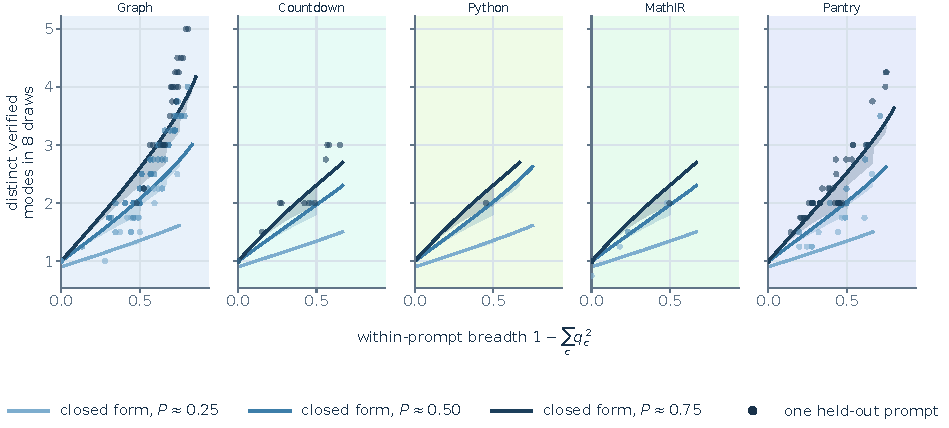
\includegraphics[width=.86\linewidth]{figures/replay_bank_decomposition.pdf}
  \caption{\textbf{Uniform allocation maximizes sampled diversity at fixed buffered probability mass.}
  The horizontal axis traces allocations from a single mode to a uniform
  distribution over $k$ buffered keys. Dashed curves show $1-(1-P)^8$, the
  probability of sampling at least one buffered key when their total mass is
  $P$. Solid curves show the expected number of distinct buffered keys for
  $P\in\{.25,.50,.75\}$; bands span a range of mode counts based on the
  observed prompts and are analytic ranges rather than confidence intervals.
  Points show held-out Level-1 prompts, which have no replay buffer, evaluated
  at the final Re:Dr and
  Re:Max checkpoints of Qwen2.5-0.5B, using one matched seed and grouping
  prompts by their verified response fraction. Their horizontal coordinates
  use empirical key frequencies in $1-\sum_c q_c^2$, rather than the unbiased
  pair estimator. Both coordinates use the same sampled responses, so the
  scatter illustrates agreement with the analytic relationship rather than
  an independent prediction of diversity on new responses.}

  \label{fig:replay-bank-decomposition}
\end{figure}

These properties describe the categorical objective on training-prompt buffers.
Generalization is measured on held-out prompts, whose responses never enter
the buffers. The surrogate alone does not establish that the implemented
response-level objective increases held-out \pmd{}.

% Shared long-paper and workshop benchmark/protocol appendix.

\clearpage
\phantomsection
\begin{center}\large\textbf{Part II. Benchmark and method}\end{center}
\addcontentsline{toc}{part}{Part II. Benchmark and method}

\section{Benchmark and Evaluation Protocol}
\label{app:data}
\label{app:experimental-design}
\label{app:domain-overview}
\label{app:data-inventory}

\mb{} uses a single executable validator to determine correctness and
solution identity, through the map $V(\cdot,s_x)$ defined in
App.~\ref{app:metric-details}. Invalid outputs receive reward zero and no
key; valid outputs receive reward one and a canonical execution key. The
valid-key catalogue and its size are unavailable to the learner and are not
used to schedule replay or determine when training stops.
Table~\ref{tab:tasks} summarizes the five domains and the response variants
that share a key. The datasets are available in the
\href{https://huggingface.co/datasets/od2961/ModeBench}{public release};
the training comparisons in this paper cover Levels 1--3.

\begin{table}[!htbp]
  \centering
  \caption{\textbf{Executable solution identities in the five \mb{} domains.}
  The validator determines both correctness and identity, while the catalogue
  of valid modes is unavailable during training. \emph{Valid modes} reports
  the mean and range of certified catalogue sizes over the Level-1 evaluation
  split. These catalogues need not include every accepted output:
  \texttt{Countdown}, for example, accepts valid keys outside its enumeration.
  \emph{Reached} reports mean distinct verified modes from one hosted
  deployment using 512 draws on 32 prompts
  per domain (Fig.~\ref{fig:gpt56-sampling-budget}). These prompts were
  selected from the evaluation split independently of model outputs. The two
  columns therefore summarize the full split and a subset, respectively.
  \texttt{MathIR}'s catalogue includes longer derivations; limited observed
  coverage does not establish whether these routes are inaccessible or simply
  too rare to observe at the given budget. Higher levels have different
  constructions and mode-count distributions (App.~\ref{app:data-levels}).
  The full prompts and model-specific chat templates appear in App.~\ref{app:prompts}.}

  \label{tab:tasks}
  \scriptsize
  \setlength{\tabcolsep}{5pt}
  \renewcommand{\arraystretch}{1.08}
  \begin{tabularx}{\linewidth}{@{}l
      >{\hsize=1.3\hsize}Y
      >{\hsize=.8\hsize}Y
      >{\hsize=.9\hsize}Y
      rr@{}}
    \toprule
    \textbf{Domain} & \textbf{Generated answer / check} &
    \textbf{Executed key} & \textbf{Equivalent responses} &
    \textbf{Valid modes} & \textbf{Reached} \\
    \midrule
    \texttt{Graph} coloring & Complete assignment; check fixed colors and edges &
    Color vector & Spacing only & 6.27 & 2.53 \\
      & & & & {\scriptsize4--12} & \\
    \addlinespace[2pt]
    \texttt{Countdown} & Parse operands; execute exactly &
    Normalized AST & Commutative order & 4.52 & 3.47 \\
      & & & & {\scriptsize2--8} & \\
    \addlinespace[2pt]
    \texttt{Python} factors & Execute restricted lambda externally &
    Return vector & Programs with the same return vector & 229.44 & 3.75 \\
      & & & & {\scriptsize16--1{,}512} & \\
    \addlinespace[2pt]
    \texttt{MathIR} & Execute bounded action program &
    State trajectory & Programs with the same states & 5.00 & 1.91 \\
      & & & & {\scriptsize5} & \\
    \addlinespace[2pt]
    \texttt{PantryPlan} & Exact ingredient allocation; check all bounds &
    Ingredient support & Quantity and ordering aliases & 18.19 & 6.91 \\
      & & & & {\scriptsize8--40} & \\
    \bottomrule
\end{tabularx}
\end{table}


\subsection{Solution mode definitions and concentration by domain}
\label{app:mode-keying}

\mb{} defines solution modes through three kinds of executable identity.
In \texttt{Countdown} and \texttt{MathIR}, distinct modes are different routes to the same
answer. In \texttt{Python}, they are different return vectors on the public test
inputs. In \texttt{Graph} and \texttt{PantryPlan}, they are different valid answers. The
response budgets also differ (Table~\ref{tab:run-contract}): a \texttt{PantryPlan}
response is a short plan, while a \texttt{Countdown} response is a derivation.
These keys identify verified solutions, not latent reasoning processes.

\paragraph{Sensitivity to the chosen equivalence.}
The canonical key determines which responses count as distinct solutions.
A coarser, task-relevant equivalence can therefore change the measured
diversity gain. App.~\ref{app:coarser-keys} tests one such equivalence per
domain. Most contrasts persist, but the replay gain for Level-3
\texttt{Python} with the original wording falls from $.419$ to zero when
$d$ and $n/d$ are treated as the same unordered factor pair. Among the five
domains, \texttt{Python} is the most sensitive to this choice. Evidence that
the gain extends beyond the original key definitions comes from the other
domains. Training uses the original canonical keys throughout; the coarser
analysis measures sensitivity to alternative definitions of solution identity.

\paragraph{Answer-only training prompts.}
The training prompts request only the final answer
(App.~\ref{app:prompts}), with response budgets chosen accordingly.
Restricting outputs to executable answers allows the validator to determine
solution identity directly, without a learned judge or an embedding-similarity
threshold. The finite solution catalogues also provide the reference values
in Table~\ref{tab:absolute-support-references}. For example, uniform sampling
over the 64 ingredient-selection bit masks in \texttt{PantryPlan} reaches
more verified modes than any trained policy evaluated here.

The training experiments do not measure diversity in long reasoning traces.
The separate hosted-model evaluations include reasoning-enabled deployments
and also exhibit concentration (App.~\ref{app:hosted-mode-diversity}), but
these inference-only observations do not establish how training changes
reasoning behavior.

Across RLVR-only arms, the mean initial-to-terminal increase in conditional
collision is $+0.202$ for route-keyed domains over
98 seed-blocks, $+0.201$ for the behavior-keyed
domain over 15, and $+0.404$ for answer-keyed
domains over 106. All three grouped means increase, with the
largest increase in the answer-keyed group. These comparisons describe
concentration under each definition; differences between domains do not
isolate the effect of choosing a particular key.

\texttt{Countdown}'s mean collision increase is $+0.383$ over
46 seed-blocks, compared with $+0.230$ in \texttt{Graph}.
Thus concentration also occurs among different derivations of a common
answer. \texttt{MathIR} has a smaller increase, $+0.042$. Its certified
catalogue includes longer derivations that are absent from the observed
outputs (App.~\ref{app:algorithm-identity}). Their absence at the evaluated
budgets does not establish that those modes are unreachable.

\paragraph{Explicit-reasoning settings and observed solution counts.}
App.~\ref{app:hosted-reasoning-control} compares five deployments on the
same 480 prompts, with eight responses per prompt and an 8,192-token output
cap in both conditions. Disabling explicit reasoning through the provider
interface lowers overall mean \texttt{distinct@8} in all five deployments:
GPT-5.6 Sol changes from 1.62 to 0.99 and GPT-5.4 from 1.85 to 1.18.
These counts include unsolved prompts and depend on both correctness and
allocation among verified solution modes. Changes in success-conditional
\pmd{} differ across deployments, so lower raw counts do not establish a
common increase in conditional concentration. The requested setting does
not establish the absence of hidden computation, and collection times and
provider defaults can also differ. This comparison therefore describes
solution distributions under the tested configurations, without identifying
an isolated effect of internal deliberation.

\subsection{Dataset splits and validation}
\label{app:data-materialization}

Each domain has disjoint training and evaluation splits
(Table~\ref{tab:run-contract}). \texttt{PantryPlan} and Level 2 also include
separate development splits (App.~\ref{app:data-levels}). For every
\texttt{Python} problem, execution verifies at least two functions with
distinct valid return vectors. For \texttt{MathIR}, each catalogue route is
checked with the same interpreter used to evaluate model outputs.

\begin{table}[!htbp]
\centering
\caption{\textbf{Dataset sizes and certified mode counts.} \texttt{Python} and \texttt{MathIR}
use disjoint training and evaluation splits. Catalogue ranges refer to the
training split; Table~\ref{tab:tasks} gives evaluation-split counts.}

\label{tab:materialization-identities}
\small
\begin{tabular}{@{}lrr@{}}
\toprule
& \textbf{\texttt{Python} factors} & \textbf{\texttt{MathIR} action menu} \\
\midrule
Training problems & 384 & 384 \\
Evaluation problems & 128 & 128 \\
Certified modes per prompt (train) & 16--3{,}600 & 5 \\
\bottomrule
\end{tabular}
\end{table}

\paragraph{\texttt{PantryPlan}.}
\label{app:data-pantry}
\texttt{PantryPlan} contains 384 training, 64 development, and 128 evaluation
prompts across four problem families. The number of feasible ingredient
supports ranges from 8--45 in training and
8--40 in evaluation, with an evaluation mean of
18.19. The validator checks inventory, serving increments, mass,
nutrient bounds, and dietary restrictions using exact arithmetic. The solution
key records which ingredients are used. These checks establish satisfaction
of the stated constraints; they do not assess taste, preparation feasibility,
or food safety.

\subsection{\texttt{Python} execution and validation}
\label{app:python}
\label{app:python-language}

After removing surrounding whitespace, the validator parses each candidate
as a Python expression, with limits of 240 characters and 64 abstract syntax
tree (AST) nodes. The accepted form is \texttt{lambda n: EXPR}, with one
ordinary argument named \texttt{n} and no default value, positional-only,
keyword, or variadic arguments. Integer literals have absolute value at most
10,000. Permitted expressions use \texttt{n}, addition, subtraction,
multiplication, floor division, remainder, integer comparisons, Boolean
\texttt{and}/\texttt{or}, unary plus/minus/\texttt{not}, and conditionals.
The validator rejects Boolean and non-integer literals, calls, imports,
attributes, comprehensions, containers, subscripts, assignment, loops, and
other identifiers.

The task specification contains $J$ distinct integers in $[4,1000]$, with
$2\le J\le8$. Every Level-1 problem uses 4 inputs drawn from
$[6,96]$ and admits at least two valid return vectors.

\paragraph{External execution.}
\label{app:python-process}
Candidate expressions run in an isolated Python process with an empty
\texttt{\_\_builtins\_\_} environment. The process repeats the syntax checks
and evaluates the function on the fixed inputs, subject to a 0.25-second
execution limit and a one-second response deadline. Timeouts, execution errors,
malformed results, non-integer outputs, and failed divisor checks produce
$\bot$ and zero reward. Only a validated integer return vector receives a key.

\paragraph{Behavioral identity.}
\label{app:python-identity}
For each of the $J$ fixed inputs $n_j$, the returned $d_j$ must be an integer
but not a Boolean, satisfy $1<d_j<n_j$, and divide $n_j$ exactly. All checks
must pass. The key is the ordered return vector $(d_1,\ldots,d_J)$;
two programs share a key exactly when these vectors agree. The exact support count
$\prod_j|\{d:1<d<n_j,\ d\mid n_j\}|$ is used only for dataset validation.

\subsection{Matched level constructions}
\label{app:data-levels}

Levels 2--5 expand the search space while preserving the verifier,
canonicalizer, and solution-mode definition. Level 2 is harder for the same
model; Levels 3--5 are calibrated against a fixed Level-1 reference using
larger models, with an exception for Level-4 \texttt{MathIR}.

\paragraph{Level 2.}
Level 2 contains 384 training, 128 development, and 128 evaluation problems,
with no shared problem identities across its splits or with Level 1.
The training distribution of valid-key counts matches that of Level 1.
For \texttt{Graph}, \texttt{Countdown}, \texttt{Python}, and \texttt{MathIR},
the development and evaluation distributions match separate Level-1 reference
sets used for dataset construction. \texttt{PantryPlan} uses its existing
Level-1 splits as references; its 64-prompt development histogram is scaled
by two to define the target counts for the 128-prompt Level-2 development set.

The Level-1 construction reference sets differ from the evaluation sets used
to compare trained policies. Consequently, those evaluation sets have different
valid-key-count distributions across levels in \texttt{Graph},
\texttt{Countdown}, and \texttt{Python}. Cross-level differences reflect both
problem structure and evaluation population, and cannot isolate difficulty
at a fixed distribution of mode counts. Within each level, replay and control
conditions use the same prompts, seeds, fresh-sample objective, and training
budget.

\begin{table}[!htbp]
\centering
\caption{\textbf{Structural differences between Levels 1 and 2.}
The verifier, canonicalizer, and definition of a solution mode are unchanged;
Level 2 expands the search space.}
\label{tab:level2-structure}
\small
\begin{tabularx}{.96\linewidth}{@{}lYY@{}}
\toprule
\textbf{Domain} & \textbf{Level 1} & \textbf{Level 2 structural change} \\
\midrule
\texttt{Graph} coloring & Three hidden vertices & Four hidden vertices \\
\texttt{Countdown} & Three operands & Four operands, with values up to 14 \\
\texttt{Python} factors & Four executed cases, all at most 96 & Four cases, including a value above 96 \\
\texttt{MathIR} & One-sided linear families & Variable-on-both-sides families \\
\texttt{PantryPlan} & Base dietary/composition constraints & More active dietary exclusions and tighter composition \\
\bottomrule
\end{tabularx}
\end{table}

On every domain's development split, fixed Qwen2.5-0.5B has
\texttt{pass@8} in $[.10,.90]$, below its Level-1 construction reference
when both levels use identical decoding settings.

\paragraph{Scale-calibrated Level 3.}
Level 3 is calibrated using Qwen2.5-3B, with Qwen2.5-0.5B on Level 1 as the
reference. Model weights remain fixed. Construction parameters are fitted
on development problems and assessed on held-out prompts. In every domain,
the calibration requires absolute differences from the reference of at most
$.04$ in pass@1 and $.08$ in pass@8, measured using four independent groups
of eight samples per prompt. \distk{} is excluded from the fitting objective.

Both models use their native chat templates, temperature 1, top-$p$ 1, and a
192-token generation limit. \texttt{Graph} prompts request only a boxed final
answer. The other domains receive task-specific solution guidance and use
decoding constrained to legal output syntax, without filtering candidates by
correctness. These criteria establish an empirical match to the reference
success rates rather than a formal two-sided equivalence test.
The Level-3 \texttt{Python} hint ablation removes the strategy guidance
(App.~\ref{app:prompt-hint-ablation}); its difficulty is therefore outside
the scope of this calibration.

\paragraph{Levels 4 and 5.}
Levels 4 and 5 are calibrated with 7B and 14B models, respectively, against
the same Qwen2.5-0.5B Level-1 reference, using pass@1 and pass@8 tolerances
of $.04$ and $.08$.
Level 5 meets these criteria in all five domains. Level 4 meets them in \texttt{Graph},
\texttt{Countdown}, \texttt{Python}, and \texttt{PantryPlan}, but not \texttt{MathIR}.

For \texttt{MathIR}, the reference pass@8/pass@1 ratio is $5.50$, whereas
the largest ratio among the evaluated 7B constructions is $4.16$. A ratio
of mixture means cannot exceed the largest component ratio, so mixing these
constructions cannot reproduce the reference ratio exactly.

The heterogeneity gap, $1-(1-\bar P)^8-\overline{\texttt{pass@8}}$, compares
observed pass@8 with its value if every prompt had the same correctness
$\bar P$. The measured gaps are $.169$--$.398$ at 7B and $.060$ for the
reference. Because the gap depends on mean correctness $\bar P$, these values
are not directly comparable across correctness levels. Each Level-4 domain
contains 384 training, 128 development, and 128 evaluation prompts, disjoint
from other levels. Level-4 \texttt{MathIR} appears in
Figs.~\ref{fig:base-levels-all-scales} and~\ref{fig:level-construction}
but is not difficulty-matched to the reference.

\subsection{Model performance across all five levels}
\label{app:base-levels-all-scales}

Fig.~\ref{fig:base-levels-all-scales} compares Qwen2.5-Instruct across five
levels and domains; Fig.~\ref{fig:families-appendix} adds three model families,
for 375 model--domain--level measurements before benchmark training.
Each measurement uses the same 128 held-out prompts per domain and level,
with four independent groups of eight responses per prompt, totaling 4,096
responses. For \texttt{pass@8} and \distk{}, we score each group, average
within prompts, and then average prompts. For \pmd{}, we pool the four
groups within each prompt (App.~\ref{app:metric-sampling}).

Evaluation uses native chat templates, temperature 1, top-$p=1$, and a
192-token output limit. \texttt{Graph} prompts request boxed final answers;
other domains use task-specific solution guidance and syntax-constrained
decoding. These settings differ from the training evaluations: under the
training template and its larger sample, the same untrained Level-1
\texttt{Python} model defines \pmd{} on 73 of 128 prompts, with mean $.168$
(Section~\ref{sec:results-collapse}). Training effects are therefore measured
against the untrained model under the corresponding evaluation conditions.

Success does not necessarily decrease monotonically with level.
\texttt{pass@8} at the highest evaluated level is below its Level-1 value in
33 of 35 model--domain series. Model scale and
benchmark level also affect diversity differently: the median range of
\pmd{} across scales at a fixed level is .251, compared with
.104 across levels at a fixed scale.

\begin{figure}[!htbp]
  \centering
  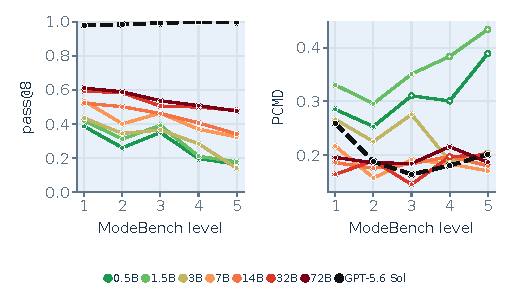
\includegraphics[width=.62\linewidth]{figures/qwen_level_trends.pdf}
  \caption{\textbf{Accuracy and solution diversity vary differently across benchmark levels.}
  Left: \texttt{pass@8}; right: \pmd{}, averaged with equal domain weights
  for each Qwen2.5-Instruct scale (colored lines) and GPT-5.6 Sol (black dashed
  line). This Qwen evaluation augments the 128 held-out prompts with the 384
  training-split prompts where available; none were used to train these
  checkpoints. Filled diversity markers indicate at least 30 prompts with
  two or more correct responses in every domain. Hollow markers average the
  available estimates when at least one domain has insufficient support;
  the set of contributing domains can differ when an estimate is undefined.}

  \label{fig:qwen-level-trends}
\end{figure}

\begin{figure}[!htbp]
  \centering
  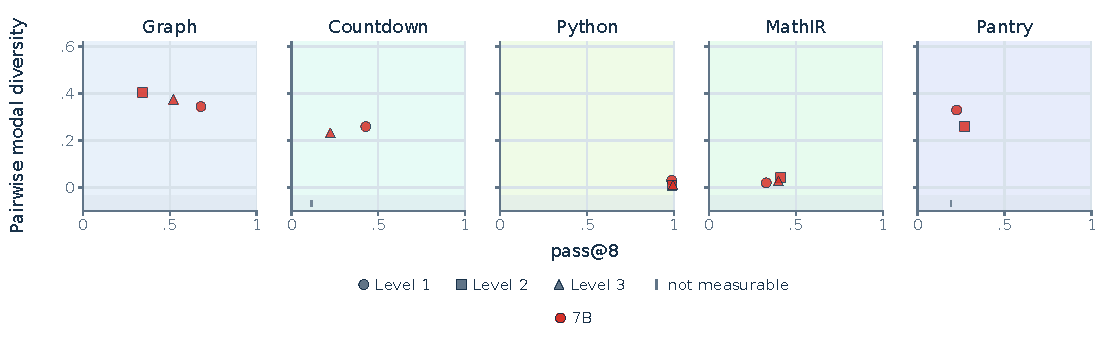
\includegraphics[width=\linewidth]{figures/mode_diversity_level_construction.pdf}
  \caption{\textbf{High accuracy can coexist with low solution diversity.}
  Each row shows one checkpoint before benchmark training, with domains in
  columns, \texttt{pass@8} on the horizontal axis, and \pmd{} on the vertical
  axis. Color indicates parameter count and marker shape indicates level.
  Each measurement uses four groups of eight responses to 128 held-out
  prompts at temperature 1; \pmd{} pools the groups within each prompt.
  Filled markers indicate at least 30 prompts with two or more correct
  responses. Hollow markers indicate 5--29 such prompts and show one standard
  error. Ticks below the axis mark measurements with fewer than five eligible prompts.}

  \label{fig:level-construction}
\end{figure}

\begin{figure}[!htbp]
  \centering
  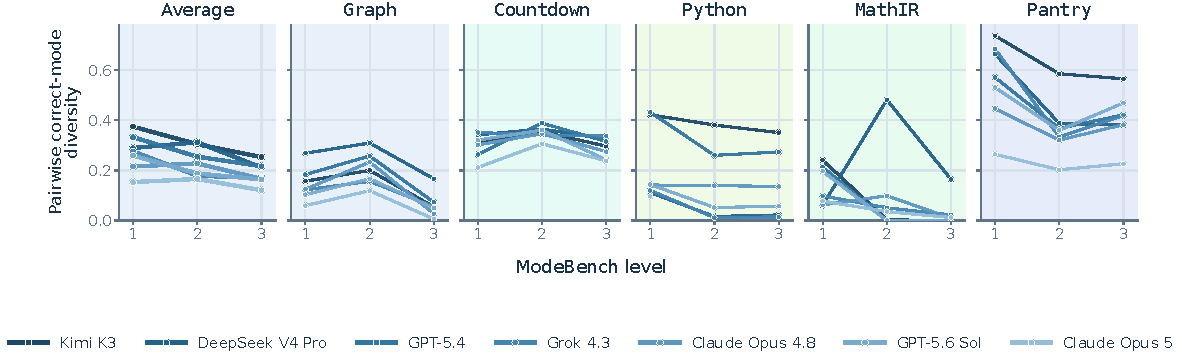
\includegraphics[width=\linewidth]{figures/frontier_level_grid.pdf}
  \caption{\textbf{Mean solution diversity is lower at Level 3 than at Level 1 for every evaluated hosted deployment.}
  Lines show \pmd{} for 7 deployments, with eight
  responses to each of 128 held-out prompts per domain and level. Panels show
  individual domains and their equally weighted mean. For each deployment,
  the set of domains contributing to the mean is fixed across levels.
  Darker lines indicate higher overall diversity. Hollow markers fall below
  the 30-prompt support threshold and are excluded from connecting lines.
  Higher levels change problem structure and add strategy guidance in
  \texttt{MathIR}, \texttt{Python}, and \texttt{PantryPlan}
  (App.~\ref{app:prompt-hint-ablation}); these curves reflect both changes.}

  \label{fig:frontier-level-grid}
\end{figure}

\begin{figure}[!htbp]
  \centering
  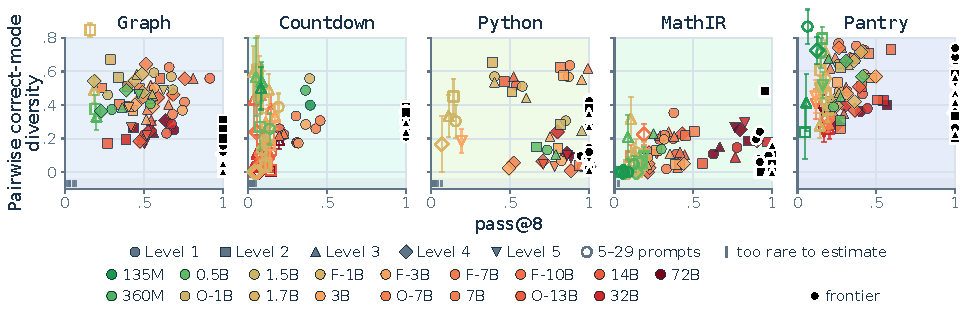
\includegraphics[width=.92\linewidth]{figures/mode_diversity_families_appendix.pdf}
  \caption{\textbf{Models of similar size can differ in solution diversity.}
  SmolLM2, Qwen2.5, Falcon3, and OLMo-2 checkpoints are compared by
  \texttt{pass@8} and \pmd{} across five domains and the available levels,
  before benchmark training. Color indicates parameter count on a logarithmic
  scale; marker shape indicates level. Black markers show the
  7 hosted deployments. Local models use four groups
  of eight responses to 128 held-out prompts per domain and level; hosted
  deployments use eight responses per prompt. Filled markers indicate at
  least 30 prompts with two or more correct responses. Hollow markers
  indicate 5--29 and show one standard error. Ticks below the axis indicate
  fewer than five eligible prompts, for which no diversity estimate is reported.}

  \label{fig:families-appendix}
\end{figure}


\FloatBarrier
\subsection{Other model families at matched scale}
\label{sec:families-appendix}

Fig.~\ref{fig:families-appendix} compares SmolLM2, Qwen2.5, Falcon3, and
OLMo-2 on the same 128 held-out prompts per domain and level. All use four
groups of eight responses, the same verifier, and the same eligibility
thresholds. Comparisons across families use the 4 shared
levels; only Qwen2.5 is evaluated at Level 5. Color denotes parameter count.

Families differ in diversity even at similar parameter counts. Near 7B,
Qwen2.5, Falcon3, and OLMo-2 have different \pmd{} values despite similar
\texttt{pass@8}. Their ordering persists in the 10--15B range, where Falcon3
and OLMo-2 are close. Within parameter-count bands, the median range of
\pmd{} across family means is .166, compared with
.198 across scales within a family, over the
4 shared levels. The earlier .251 summary instead
compares all seven Qwen scales at each level. These descriptive comparisons
do not isolate which pretraining or post-training choices account for the
differences between models.

\clearpage
\subsection{Training and evaluation settings}
\label{app:repro-run-contract}
\label{app:comparison-design}

% [H] pinned this table to the head of the subsection, and being too tall for
% what the previous page had left it took a page of its own and stranded the
% remainder. Floating lets the prose that follows it close the gap.
\begin{table}[!htbp]
  \centering
  \caption{\textbf{Paired comparisons use the same numbers of optimizer updates and fresh rollouts.}
  Treatment and control share the settings below. Both compute replay scores
  and execute the backward pass, but the replay gradient is exactly zero in
  the control. Their buffer contents can differ, so replay workloads, total
  floating-point operations, and wall-clock time are not matched. The control
  receives no additional training in place of replay computation
  (App.~\ref{app:compute-matching}).}

  \label{tab:run-contract}
  \small
  \begin{tabularx}{\linewidth}{@{}P{.23\linewidth}Y@{}}
    \toprule
    \textbf{Component} & \textbf{Setting} \\
    \midrule
    Data & 384 training and 128 disjoint evaluation prompts per domain and
      level; evaluation prompts are excluded from training and replay. \\
    Fresh rollouts & $G=16$, temperature 1, top-$p=1$; one prompt group per update. \\
    Optimization & Eight training passes (3,072 updates), with one PPO epoch
      per batch. $\beta_{\mathrm{KL}}=0$ except in the reference-KL comparison
      (App.~\ref{app:kl-measured}), which varies only this coefficient.
      Paired conditions share initialization, prompt order, optimizer,
      hardware class, and checkpoint frequency. \\
    Evaluation & At passes $0,.5,\ldots,8$: four groups of eight responses
      per prompt at temperature 1 and top-$p=1$, plus a separate greedy
      response at temperature 0. Final comparisons use the last checkpoint. \\
    Replay & Capacity $M=16$ keys per prompt; buffers are selected in
      round-robin order, one per update; $\lambda_{\mathrm{replay}}=.10$.
      The control has zero replay gradient; buffer contents and computational
      workloads may differ between conditions. \\
    Training seeds & Five per model--domain combination; paired comparisons use
      common seeds, with sample sizes reported alongside the results. \\
    Learning rate & Qwen2.5-0.5B and Falcon3-1B: constant $2\times10^{-7}$,
      with Falcon optimizer states stored on the CPU. Qwen2.5-3B: cosine
      decay from a $10^{-7}$ peak to a $10^{-8}$ floor, with 10\% warmup. \\
    Optimizer & Fused Adam in \texttt{bf16} with decoupled weight decay,
      $\beta_1=.9$, $\beta_2=.95$, weight decay $0$, gradient-norm clip $1.0$,
      with gradient checkpointing. CPU offloading uses the corresponding
      CPU optimizer implementation with the same hyperparameters. \\
    Policy update & Parameters are synchronized after every update, and each
      rollout is used once in a single PPO epoch. The symmetric clipping
      threshold is $\varepsilon=.2$. The importance ratio equals $1$ when
      the surrogate is evaluated in this update scheme, so clipping is inactive. \\
    % All twelve cells are the OAT_ZERO_GENERATE_MAX_LENGTH actually submitted,
    % read per domain from the job ledgers rather than from a launcher default:
    %   0.5B  var/artifacts/e72_frontier_source_runs.json
    %           (inherited_eval_config.generate_max_length; the 3B cohort
    %            inherits this record and overrides only the base model)
    %   1B    var/artifacts/e79_falcon1b_aligned_verified_replay_jobs.json
    %   3B    var/artifacts/e80r1_qwen3b_aligned_verified_replay_jobs.json
    % ops/train.sh defaults this to 192, so a domain that is 192 looks the same
    % whether it was chosen or inherited; the ledgers are what distinguish them.
    Response tokens & \texttt{Graph} and \texttt{Countdown}: 192; \texttt{Python}: 192/512/192
      at 0.5B/1B/3B; \texttt{MathIR}: 64/128/64; \texttt{PantryPlan}: 8. \\
    \bottomrule
  \end{tabularx}
\end{table}



For each training seed, \texttt{pass@8} and \texttt{distinct@8} are averaged
over four eight-response groups per prompt and all 128 evaluation prompts;
\texttt{mean@8} is the fraction of correct responses. Responses are independent
within a group. Independence across groups, required for the pooled \pmd{}
interpretation, depends on the sampling procedure described in
App.~\ref{app:metric-sampling}. Evaluation outputs are excluded from training
and replay, and do not determine checkpoint selection or stopping.

Comparisons use paired final checkpoints. Comparisons with five matched
training seeds use nominal pointwise 95\% Student-$t$ intervals; other main
checkpoint comparisons report sample sizes and descriptive means. Diversity
comparisons use the prompt-eligibility thresholds and interval procedures
specified alongside their results. Intervals condition on the fixed evaluation
prompts and sampled responses. The replay-weighting comparison instead uses
a bootstrap over paired training seeds.

% Finish benchmark floats before beginning the prompt examples.
\FloatBarrier
\section{Exact Domain Prompts}
\label{app:prompts}

Each domain's training prompt contains one system message and one user
message, without few-shot examples. Training and evaluation use the same
template within each method. The examples below reproduce the first prompt
from each Level-1 evaluation split in Qwen's chat format. Falcon3 uses the
same message text with its own \texttt{<|system|>} and \texttt{<|user|>}
markers. Models evaluated before benchmark training use their tokenizer's
native chat template (App.~\ref{app:base-levels-all-scales}).
App.~\ref{app:data-levels} describes the different problems and prompting
conditions at Levels 2--5.

The examples preserve the prompt text. A continuation line indented by two
spaces indicates a display line break; replacing that break and indentation
with one space recovers the original text. In the \texttt{PantryPlan}
example, a line break without this indentation is part of the prompt.

% BEGIN generated by ops/check_paper_domain_prompts.py

\filbreak
\subsection{\texttt{Graph} coloring}
\label{app:prompt-graph}

\noindent 384 training and 128 evaluation prompts.

\begin{Verbatim}[fontsize=\scriptsize,frame=single,framesep=4pt,rulecolor=\color{black!25},samepage=true]
<|im_start|>system
Return only the final answer inside \boxed{}. Do not explain.<|im_end|>
<|im_start|>user
Color this graph with vertices 1 through 6. The undirected edges are: (1,2), (1,3),
  (3,5), (3,6), (4,6), (5,6). Assign each vertex one color from {1, 2, 3} so that no
  edge has the same color on both endpoints. A partial coloring is 2??1?2, where ?
  means uncolored. Keep every shown digit fixed. There are exactly 3 question marks.
  Return exactly one final answer and no explanation: exactly 3 digits, each one 1,
  2, or 3, for the missing positions from left to right, inside \boxed{}.<|im_end|>
<|im_start|>assistant
\end{Verbatim}

\filbreak
\subsection{\texttt{Countdown}}
\label{app:prompt-countdown}

\noindent 384 training and 128 evaluation prompts.

\begin{Verbatim}[fontsize=\scriptsize,frame=single,framesep=4pt,rulecolor=\color{black!25},samepage=true]
<|im_start|>system
Return only the final answer inside \boxed{}. Do not explain.<|im_end|>
<|im_start|>user
Using the numbers [3, 6, 9], create an arithmetic expression that equals 18. Use
  each given number exactly once. You may use +, -, *, /, and parentheses. Return
  exactly one final answer and no explanation: the expression inside
  \boxed{}.<|im_end|>
<|im_start|>assistant
\end{Verbatim}

\filbreak
\subsection{\texttt{Python} factors}
\label{app:prompt-python}

\noindent 384 training and 128 evaluation prompts.

\begin{Verbatim}[fontsize=\scriptsize,frame=single,framesep=4pt,rulecolor=\color{black!25},samepage=true]
<|im_start|>system
Return only the final answer inside \boxed{}. Do not explain.<|im_end|>
<|im_start|>user
Write one pure Python function with the exact form lambda n: EXPR. An external
  Python tool will call it once for each n in [18, 82, 91, 93]. For every call,
  return an integer d satisfying 1 < d < n and n % d == 0. Different valid return
  vectors are different solution modes. You may use integer literals, n, +, -, *,
  //, %, comparisons, Boolean operators, and conditional expressions; calls,
  imports, attributes, containers, and other names are forbidden. Return exactly the
  one-line lambda inside \boxed{} and no explanation.<|im_end|>
<|im_start|>assistant
\end{Verbatim}

\filbreak
\subsection{\texttt{MathIR} action menu}
\label{app:prompt-mathir}

\noindent 384 training and 128 evaluation prompts.

\begin{Verbatim}[fontsize=\scriptsize,frame=single,framesep=4pt,rulecolor=\color{black!25},samepage=true]
<|im_start|>system
Return only the final answer inside \boxed{}. Do not explain.<|im_end|>
<|im_start|>user
MathIR linear-menu-v1. Solve for x by choosing an executable action sequence. Every
  selected action is applied exactly to BOTH sides of the current equation, followed
  by exact simplification. Bindings: a=2, b=-9, c=-1. Initial equation: x/a + b = c.
  Action menu: A means div(a); B means add(b); C means sub(b); D means sub(c); E
  means sub(mul(a,b)); F means mul(a). Choose 1-4 action IDs. Illegal operations,
  repeated states, and paths that do not finish with x isolated are rejected. Return
  only the IDs separated by semicolons inside the answer box; for example formatting
  only: \boxed{A;C}. Do not return x's numeric value.<|im_end|>
<|im_start|>assistant
\end{Verbatim}

\subsection{\texttt{PantryPlan}}
\label{app:prompt-pantry}

\noindent 384 training and 128 evaluation prompts.

\begin{Verbatim}[fontsize=\scriptsize,frame=single,framesep=4pt,rulecolor=\color{black!25},samepage=false]
<|im_start|>system
Return only six binary digits and no other text. Each digit maps to the
  corresponding Pantry row in printed order. A trusted environment will choose exact
  quantities on precisely the selected rows.<|im_end|>
<|im_start|>user
Create one feasible high fiber snack from this frozen pantry.
Nutrition values are per 100 g. Quantities are exact integer grams.

Pantry:
- almonds: available=100g, step=25g, minimum-if-used=50g; energy=584kcal,
  protein=21.5g, fiber=10.8g, sodium=0.0mg; tags=tree_nut
- banana: available=125g, step=25g, minimum-if-used=50g; energy=97.0kcal,
  protein=0.74g, fiber=4.62g, sodium=0.0mg; tags=none
- carrots: available=150g, step=25g, minimum-if-used=50g; energy=45.0kcal,
  protein=0.941g, fiber=3.1g, sodium=86.6mg; tags=none
- grape_tomatoes: available=100g, step=25g, minimum-if-used=50g; energy=27.0kcal,
  protein=0.83g, fiber=2.1g, sodium=6.0mg; tags=none
- navel_orange: available=150g, step=25g, minimum-if-used=50g; energy=47.0kcal,
  protein=0.91g, fiber=2.0g, sodium=9.0mg; tags=none
- sunflower_seeds: available=125g, step=25g, minimum-if-used=50g; energy=571kcal,
  protein=18.9g, fiber=7.22g, sodium=0.0mg; tags=none

Use 2 to 4 ingredients.
Forbidden tags: none
Targets:
- mass_g: minimum 125, maximum 200
- energy_kcal: minimum 239.4, maximum 432.25
- protein_g: minimum 6.423
- fiber_g: minimum 3.478
- sodium_mg: maximum 37.6

Choose the ingredient support as a six-bit mask in the exact Pantry row order. Bit 1
  includes that row and bit 0 excludes it.<|im_end|>
<|im_start|>assistant
\end{Verbatim}

% END generated by ops/check_paper_domain_prompts.py

% Shared exact replay update; empirical comparisons are in results.tex.

\section{Replay Algorithm}
\label{app:algorithm}

Verified replay combines learning from newly sampled responses with a
likelihood loss on stored, verified solutions. Each prompt $x$ has a buffer
$\mathcal B_x$ of at most $M$ exemplars, with one response per canonical key.
A round-robin cursor $\sigma$ selects one prompt's buffer at each update,
and all keys in that buffer contribute equally to the replay loss.
Table~\ref{tab:notation} defines the notation;
App.~\ref{app:replay-metric-alignment} relates this objective to diversity.

\subsection{Fresh task advantages}
\label{app:binary-maxrl}

For a group of $G$ fresh responses with verified binary rewards $R_i$ and
$R=\sum_i R_i$, Dr.GRPO uses $A_i=R_i-R/G$, while MaxRL uses
\[
 A_i^{\mathrm{MaxRL}}=
 \begin{cases}
 G R_i/R-1, & R>0,\\
 0, & R=0.
 \end{cases}
\]
The centered MaxRL estimator \citep{tajwar2026maxrl} assigns advantage $-1$
to failures in mixed groups and gives each success greater weight when
successes are scarce. Both objectives assign zero task advantage to every
response in an all-correct or all-failure group. Lemma~\ref{lem:maxrl-mean}
derives MaxRL's mean objective as a harmonic combination of pass@\(k\)
terms. These advantages apply to fresh responses; stored exemplars contribute
through the separate replay loss.

\subsection{Optimizer update}
\label{app:algorithm-update}

\begin{algorithm}[H]
  \caption{\textbf{Verified replay update.} The fresh objective selects Re:Dr or Re:Max.}
  \label{alg:verified-replay-update}
  \small
  \begin{algorithmic}[1]
    \REQUIRE Policy $\pi_\theta$; prompt $x$ and verifier specification
      $s_x$; group size $G$; fresh objective
      $o\in\{\mathrm{MaxRL},\mathrm{Dr.GRPO}\}$; replay weight
      $\lambda_{\mathrm{replay}}$; buffer capacity $M$; buffers and cursor
      $(\mathcal B,\sigma)$
    \ENSURE Updated $(\theta',\mathcal B',\sigma')$
    \STATE Draw the on-policy group
      $\mathcal G=\{y_i\sim\pi_\theta(\cdot\mid x)\}_{i=1}^G$
    \FOR{$i=1,\ldots,G$}
      \STATE Execute $\widetilde c_i\gets V(y_i,s_x)$ and observe task
        reward $R_i$
      \STATE Set $c_i\gets\widetilde c_i$ iff
        $R_i>0\wedge\widetilde c_i\ne\bot$; otherwise set $c_i\gets\bot$
    \ENDFOR
    \STATE Compute fresh task advantages $A_i^{o}$ from $\{R_j\}_{j=1}^G$;
      for $o=\mathrm{MaxRL}$ use the formula in App.~\ref{app:binary-maxrl}
    \STATE After the full group is validated, deterministically retain one
      policy exemplar for each new $c_i\ne\bot$ in $\mathcal B_x$, up to
      capacity $M$
    \STATE $(z,\sigma')\gets\textsc{NextBuffer}
      (\{\mathcal B_u\}_u,\sigma)$ by a fixed round-robin cursor over
      prompts; the replayed prompt $z$ need not be the prompt $x$ that
      supplied the fresh group
    \IF{a replay buffer $\mathcal B_z$ exists}
      \STATE For each exemplar $e_c\in\mathcal B_z$, compute
        $\ell_c=|e_c|^{-1}\log\pi_\theta(e_c\mid z)$
      \STATE $L_{\mathrm{replay}}\gets-|\mathcal B_z|^{-1}
        \sum_{c\in\mathcal B_z}\ell_c$
    \ELSE
      \STATE $L_{\mathrm{replay}}\gets0$
    \ENDIF
    \STATE Set the replay-loss normalization $w_{\mathrm{rep}}\gets(G-1)/G^2$
    \STATE $\theta'\gets\textsc{Update}
      (\theta,L_{\mathrm{PPO}}(A^{o})
      +w_{\mathrm{rep}}\lambda_{\mathrm{replay}}L_{\mathrm{replay}})$
\end{algorithmic}
\end{algorithm}

\subsection{Buffer construction and scheduling}
\label{app:algorithm-bank}

Each buffer is associated with an exact prompt-token sequence. A response
is eligible for storage if it has positive task reward and a valid canonical
key, including responses that reach the generation limit. The entire group
is validated before the buffer is updated. For each newly observed key, we
retain the lexicographically smallest normalized response-token sequence;
new keys are inserted in sorted order. Selection therefore does not depend
on the order of responses within the group. Each buffer holds at most
$M=16$ exemplars, one per key, with no eviction or replacement. Keys first
observed after the buffer is full receive no replay support.

At each update, a deterministic round-robin schedule selects one nonempty
buffer, including buffers containing a single exemplar. The choice does not
use reward magnitudes, evaluation results, a target mode count, or entropy.
The policy scores every stored response in the selected buffer by teacher
forcing, conditioned on its original prompt. Each exemplar contributes its
mean response-token log probability, excluding prompt and padding tokens.

The replay loss is the negative mean score over the selected keys,
weighted by $\lambda_{\mathrm{replay}}(G-1)/G^2$
(Algorithm~\ref{alg:verified-replay-update}). The normalization $(G-1)/G^2$
matches the weight of a single success in a centered Dr.GRPO group: its
advantage is $(G-1)/G$, followed by averaging over $G$ responses
(Lemma~\ref{lem:grpo-mean}). This loss uses only discovered training
exemplars; it requires neither the complete valid-key catalogue nor
evaluation outputs.

\subsection{Control without replay gradients}
\label{app:algorithm-control}

Replay and control use the same validation, buffer construction, scheduling,
and exemplar-scoring procedures. The control sets the replay gradient to
zero while retaining the forward and backward computations. Both conditions
combine the fresh-task and replay gradients in one optimizer step; the
replay gradient is their only difference in the learning objective.

As the policies diverge, they can generate different responses and accumulate
different buffers, which changes the selected exemplars and their lengths.
The conditions match optimizer updates and fresh-rollout budgets, but not
realized floating-point operations or wall-clock time. The control receives
no additional task-gradient updates, fresh rollouts, or training time in
place of replay computation. The comparison isolates the contribution of the
replay learning signal under this design, without establishing an advantage
at equal total compute (App.~\ref{app:compute-matching}).

\subsection{Verifier requirements and applicability}
\label{app:algorithm-identity}

Replay requires a deterministic rule for grouping verified responses into
solution modes. Its canonical key must be computable for every training
response at reasonable cost and must reflect the task's definition of a
solution. In \mb{}, one executable validator determines both correctness
and identity, so buffer construction requires no learned judge or
embedding-similarity threshold.

Final-answer grading, as used for MATH, GSM8K, and AIME, does not distinguish
derivations of the same answer. When a prompt has only one correct answer,
an answer-based key places every successful response in the same mode. The
buffer then holds one exemplar, and replay reinforces it without balancing
alternative derivations. That buffer is the capacity-one arm of
App.~\ref{app:mode-agnostic-replay}, which retains 58\% of the
Re:Dr diversity effect and a correctness gain of +.263 against
Re:Dr's +.352. Measuring and replaying distinct derivations
requires a finer definition of identity.

\texttt{MathIR} uses executed state trajectories as keys. Its catalogue
includes verified four-state routes, but none appears among 27,450
verified draws. Across 115 solved Level-1 prompts, these
draws cover 67\% of the certified two-state modes and
52\% of the three-state modes. Different modes rarely appear
for the same prompt. Terminal \pmd{} averages .006, corresponding
to 1.01 effective verified modes per prompt. These results provide
limited evidence for diversity gains among alternative derivations.

Across the 6 comparisons, including \texttt{MathIR} in the
five-domain mean reduces the \pmd{} gain by .010--.074
relative to the corresponding four-domain mean. At Qwen2.5-0.5B, the Re:Dr
gain is +.294 across all five domains and +.364 across the other
four. App.~\ref{app:hosted-mode-diversity} reports hosted-model results for
the same four-domain subset.

For open-ended derivations, a learned judge could supply a novelty criterion,
but that criterion would require independent validation. Judge decisions can
be inconsistent or disagree with task correctness, and replay may reinforce
distinctions that the judge rewards without improving solution diversity.
Fixing the judge model, prompt, and decoding rule does not by itself ensure
a valid equivalence relation. Where executable keys are available, they can
be used to assess the judge and measure diversity separately from its training
signal. We do not evaluate judge-based replay here.

\subsection{Exemplar quality and length}
\label{app:algorithm-quality}

Canonical verification establishes that a response satisfies the task
constraints. It does not validate every intermediate reasoning step: a
verified response may be verbose or include an unsound explanation. Replay
weights exemplars by solution key without ranking their reasoning quality.

Each key occupies one buffer entry and contributes its exemplar's mean
response-token log probability,
$\ell_c=|e_c|^{-1}\log\pi_\theta(e_c\mid z)$. Longer responses therefore do
not receive more buffer entries or loss weight proportional to their token
count. This normalization still affects the learning target. In a categorical
surrogate with one exemplar of fixed length $L_b$ per key, the effective
weights are proportional to $L_b^{-1}$. With full coverage, the limiting
distribution favors shorter exemplars and is uniform only when lengths are
equal (App.~\ref{app:theory-replay}). This conclusion concerns the surrogate;
mean-token normalization does not imply uniform key probabilities in a
language model or guarantee concise, sound explanations.

Additional length or reasoning-quality filters would change which exemplars
enter or remain in the buffer, and hence change the replay target. We use no
such filters beyond the stated generation limits and verification rules.
Restricting length can exclude valid alternatives: \texttt{MathIR} includes
longer state trajectories, and the observed lambdas for rarer \texttt{Python}
return vectors are longer than those for the modal vector. Evaluating a
quality filter would therefore require measuring both solution quality and
diversity among retained modes.

\section{Fixed Semantic-MaxEnt Comparator}
\label{app:semantic-maxent}

Fixed Semantic-MaxEnt adds a frequency-based bonus to the fresh-response
advantage. It counts previously observed verified keys but does not optimize
the likelihood of stored exemplars. For response $i$ in a group of $G$
responses to prompt $x$, let $n_x(a)$ count earlier successful responses
with key $a$, and let $m_{-i}(a)$ count successful responses with that key
among the other members of the current group. Write
$N_x=\sum_a n_x(a)$, $S_{-i}=\sum_a m_{-i}(a)\le G-1$, and let
$\mathcal K_i$ contain all keys observed in these two sources. Adding one
pseudocount per observed key and reserving one for unseen keys gives,
for $a\in\mathcal K_i$,

\begin{equation}
  \hat p_i(a)=\frac{n_x(a)+m_{-i}(a)+1}{N_x+S_{-i}+|\mathcal K_i|+1},\qquad
  \hat p_i(\textsc{unseen})=\frac{1}{N_x+S_{-i}+|\mathcal K_i|+1}.
  \label{eq:open-set-predictor}
\end{equation}
A response whose key is outside $\mathcal K_i$ receives the probability
assigned to the unseen category. Invalid and unsuccessful responses do not
contribute to the counts.

\paragraph{Counts and advantage calculation.}
Counts are specific to each exact prompt-token sequence and accumulate
throughout training without decay or reset. Only responses with positive
reward and a valid key are counted. Each response is scored using previous
groups and the other successful responses in its current group. Counts for
the full current group are added only after scoring, so a response never
contributes to its own predicted probability.
The added advantage for an eligible successful response is held constant
during differentiation and equals

\begin{equation}
  A^{\rm sem}_{i,t}=\eta\,
  \frac{\min\{-\log\hat p_i(a_i),\kappa\}
    -\E_{\hat p_i}[\min\{-\log\hat p_i(a),\kappa\}]}{\kappa},
  \qquad \eta=.10,\ \kappa=5.
  \label{eq:legacy-semantic-advantage}
\end{equation}
The same $A^{\rm sem}_{i,t}$ applies at every token position $t$ of response
$i$. Invalid and unsuccessful responses receive zero bonus. The fixed scale
$\eta$ bounds the centered bonus in magnitude, while $\kappa$ clips the
surprisal. The bonus can favor an underrepresented verified mode when that
mode appears in a fresh response, but it adds no direct likelihood term for
a stored exemplar absent from the group. If neither previous groups nor the other
successful responses provide a key, the unseen category has probability one
and the bonus is zero. App.~\ref{app:ucpo-progress} reports the comparison.

\paragraph{Relation to conditional entropy.}

For the true conditional distribution $q_\theta=p_\theta(\cdot\mid\mathcal C)$,
\begin{equation}
 \nabla_\theta H(q_\theta)
 =\E_{a\sim q_\theta}[(-\log q_\theta(a))\nabla_\theta\log q_\theta(a)].
 \label{eq:entropy-score-function}
\end{equation}
The frequency predictor generally does not provide an unbiased estimator
of this gradient. To see the distinction, hold a predictor score vector $s$
and baseline $b$ fixed independently of the scored action, for example by
conditioning on the other responses in its group. Averaging the gradients
of successful responses under the unconditional policy gives

\[
 \E_{Z\sim p}[\1\{Z\in\mathcal C\}(s_Z-b)\nabla_\theta\log p_Z]
 =P\E_{c\sim q}[s_c\nabla_\theta\log q_c]
   +(\E_q[s]-b)\nabla_\theta P.
\]
The predictor's baseline need not equal the current conditional mean
$\E_q[s]$. The second term can therefore change correctness as well as the
allocation among correct modes. Even with the exact, unclipped score
$s_c=-\log q_c$ and baseline $b=H(q)$, averaging over all rollout responses
yields $P\nabla_\theta H(q)$, scaled by the probability of success.

The distinction also matters when only one correct key exists. Its
conditional entropy is zero, yet probability assigned to the unseen
category can make its semantic advantage negative after it has been
observed. The bonus is therefore generally not an exact conditional-entropy
gradient, and it provides no guarantee of individual-mode preservation.

% Every part divider opens a fresh page, this one included. It used to run on
% from the comparator section to save the white space below that section's end;
% uniformity across the seven dividers is worth the part page.
\clearpage
\phantomsection
\begin{center}\large\textbf{Part III. Training results}\end{center}
\addcontentsline{toc}{part}{Part III. Training results}

\section{Empirical Results and Comparisons}
\label{app:supporting}

\begin{figure}[!htbp]
\centering
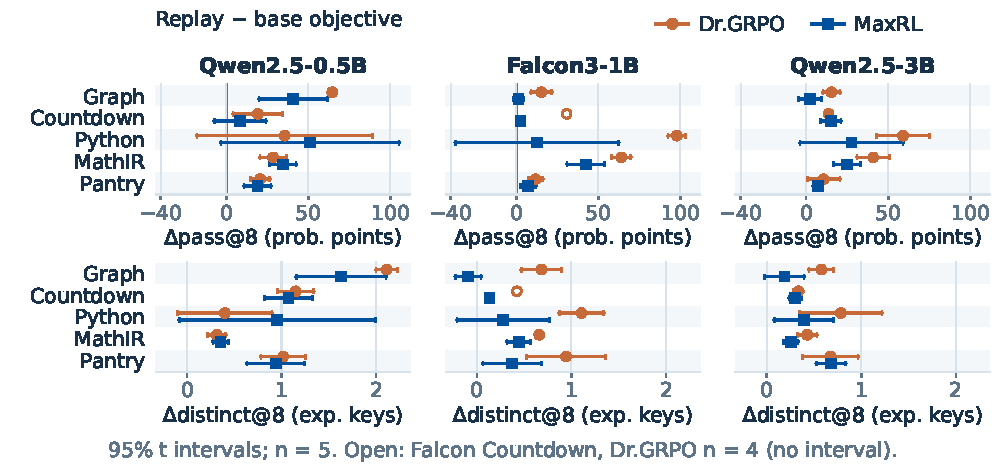
\includegraphics[width=\linewidth]{figures/replay_factorial_effects.pdf}
\caption{\textbf{Replay raises mean correctness at all three model scales.}
Final-checkpoint differences: Re:Dr minus Dr.GRPO (circles) and Re:Max minus
MaxRL (squares), measured in percentage points for \texttt{pass@8} and in
\pmd{} units for diversity. Filled markers use five paired seeds; hollow
markers use fewer. For Re:Dr, correctness uses four seeds in Falcon
\texttt{Countdown}; diversity uses four in Falcon \texttt{Countdown}, one
in Falcon \texttt{MathIR}, and two in Qwen2.5-3B \texttt{Python}. Diversity
requires at least 20 eligible prompts per arm; blanks indicate no eligible
comparison. Bars show nominal paired 95\% Student-$t$ intervals, requiring
five seeds for correctness and at least two for diversity.}
  \label{fig:replay-factorial-effects}
\end{figure}

\subsection{Terminal comparisons across scales}
\label{app:scale-matrix}
\label{app:scale-snapshot}
\label{app:maxrl-scale-extensions}
\label{app:current-campaign-results}

Paired conditions share initialization, training and evaluation prompts,
eight training passes, evaluation requests, the verifier, and replay schedule.
The control uses the same buffer construction and scoring procedures with
zero replay gradient. Policies can develop different buffers and workloads,
so total compute is not matched (App.~\ref{app:compute-matching}).

\crossscaletablematerial

\paragraph{Dr.GRPO retention contrasts.}
\label{app:retention-numerical-detail}

% Floats rather than [H] so it can rise to the page its discussion starts
% on instead of forcing a break and leaving the preceding page part empty.
\begin{table}[!tbp]
  \centering
  \caption{\textbf{Replay improves mean correctness and solution diversity at each tested scale.}
  Final-checkpoint differences between Re:Dr and Dr.GRPO, by domain and
  model. Superscripts indicate fewer than five paired seeds; dashes indicate
  no eligible comparison. Diversity effects require at least 20 eligible
  prompts per arm. Each Avg weights a fixed set of domains equally within
  seed: all five for correctness, and domains eligible for every seed for
  diversity. The diversity mean uses \texttt{Graph} and \texttt{PantryPlan}
  at Falcon3-1B, all domains except \texttt{Python} at Qwen2.5-3B, and all
  five at 0.5B. Eligible prompt subsets may differ between the two arms.}

\label{tab:cross-scale-terminal-effects}
  \scriptsize
  % Keep the two longest domain headers on two lines, as in the main table,
  % so typewriter labels retain their size within the thirteen-column layout.
  \setlength{\tabcolsep}{1.4pt}
  \renewcommand{\arraystretch}{0.92}
  \begin{tabular}{@{}l*{12}{r}@{}}
    \toprule
    & \multicolumn{6}{c}{\textbf{$\Delta$ \texttt{pass@8}}}
      & \multicolumn{6}{c}{\textbf{$\Delta$ \pmd{}}} \\
    \cmidrule(lr){2-7}\cmidrule(l){8-13}
    & \texttt{Graph} & \shortstack{\texttt{Count}\\\texttt{down}} & \texttt{Python} & \texttt{MathIR} & \shortstack{\texttt{Pantry}\\\texttt{Plan}} & Avg
      & \texttt{Graph} & \shortstack{\texttt{Count}\\\texttt{down}} & \texttt{Python} & \texttt{MathIR} & \shortstack{\texttt{Pantry}\\\texttt{Plan}} & Avg \\
    \midrule
    % Generated by build_paper_retention_matrix_tables.py; do not hand edit.
    \qwenmark{}2.5-0.5B & \cellcolor[HTML]{A9D6A0}$+.646$ & \cellcolor[HTML]{C7E0A2}$+.191$ & \cellcolor[HTML]{DBE7A4}$+.356$ & \cellcolor[HTML]{D5E4A3}$+.285$ & \cellcolor[HTML]{A9D6A0}$+.207$ & \cellcolor[HTML]{BCDCA1}$+.337$ & \cellcolor[HTML]{A9D6A0}$+.559$ & \cellcolor[HTML]{A9D6A0}$+.480$ & \cellcolor[HTML]{A9D6A0}$+.082$ & \cellcolor[HTML]{DDE7A4}$+.017$ & \cellcolor[HTML]{A9D6A0}$+.334$ & \cellcolor[HTML]{A9D6A0}$+.294$ \\
    \falconmark{}3-1B & \cellcolor[HTML]{E5EAA5}$+.153$ & \cellcolor[HTML]{A9D6A0}$+.307^{4}$ & \cellcolor[HTML]{A9D6A0}$+.979$ & \cellcolor[HTML]{A9D6A0}$+.640$ & \cellcolor[HTML]{CBE1A3}$+.118$ & \cellcolor[HTML]{A9D6A0}$+.442^{4}$ & \cellcolor[HTML]{D8E6A4}$+.224$ & \cellcolor[HTML]{F3EEA6}$+.032^{4}$ & \textemdash{} & \cellcolor[HTML]{D5E4A3}$+.022^{1}$ & \cellcolor[HTML]{ADD7A0}$+.317$ & \cellcolor[HTML]{AFD8A0}$+.271$ \\
    \qwenmark{}2.5-3B & \cellcolor[HTML]{E5EAA5}$+.154$ & \cellcolor[HTML]{D5E4A3}$+.137$ & \cellcolor[HTML]{C8E0A2}$+.590$ & \cellcolor[HTML]{C6DFA2}$+.409$ & \cellcolor[HTML]{CFE3A3}$+.106$ & \cellcolor[HTML]{C6E0A2}$+.279$ & \cellcolor[HTML]{DFE8A4}$+.176$ & \cellcolor[HTML]{E8EBA5}$+.100$ & \cellcolor[HTML]{CCE1A3}$+.046^{2}$ & \cellcolor[HTML]{E4E9A4}$+.013$ & \cellcolor[HTML]{BEDDA2}$+.247$ & \cellcolor[HTML]{D4E4A3}$+.134$ \\
    \bottomrule

  \end{tabular}
\end{table}

Tables~\ref{tab:core-terminal-endpoints} and~\ref{tab:cross-scale-terminal-effects}
report means for each condition and paired replay effects, respectively.
Adding replay to Dr.GRPO increases mean \texttt{pass@8} and \distk{} in
all 14 comparisons with five paired seeds; \distk{} increases in all 74
individual seed pairs. Because \distk{} also depends on correctness, we use
\pmd{} to measure diversity conditional on a correct response.

For Qwen2.5-0.5B, \texttt{Countdown} \texttt{pass@8} rises from $.480$ to
$.672$, with a \pmd{} gain of $+.480$ (95\% interval $[+.447,+.513]$).
\texttt{Python} correctness rises from $.172$ to $.528$, with a diversity
gain of $+.082$ ($[-.146,+.310]$). \texttt{MathIR} correctness rises from
$.512$ to $.796$, with a diversity gain of $+.017$ ($[+.003,+.031]$).
These are nominal Student-$t$ intervals over five paired training seeds,
without multiple-comparison adjustment. \texttt{Countdown}'s final \pmd{}
values are $.007$ for Dr.GRPO and $.487$ for Re:Dr. Its keys distinguish
computation routes, but these held-out evaluations do not track the survival
of particular routes discovered during training.

Fig.~\ref{fig:maxrl-factorial-scale-extensions} shows the results by domain.
Two-method effects use shared seeds; factorial interactions use seeds shared
by all four methods. Diversity comparisons additionally require enough
verified responses to estimate the conditional distribution.

% Not [H]: this plate is a full text-block tall, so forcing it here left the
% rest of the preceding page blank whenever it did not fit. Letting it float
% fills that page and keeps the plate near the text that cites it by number.
\begin{figure}[!htbp]
  \centering
  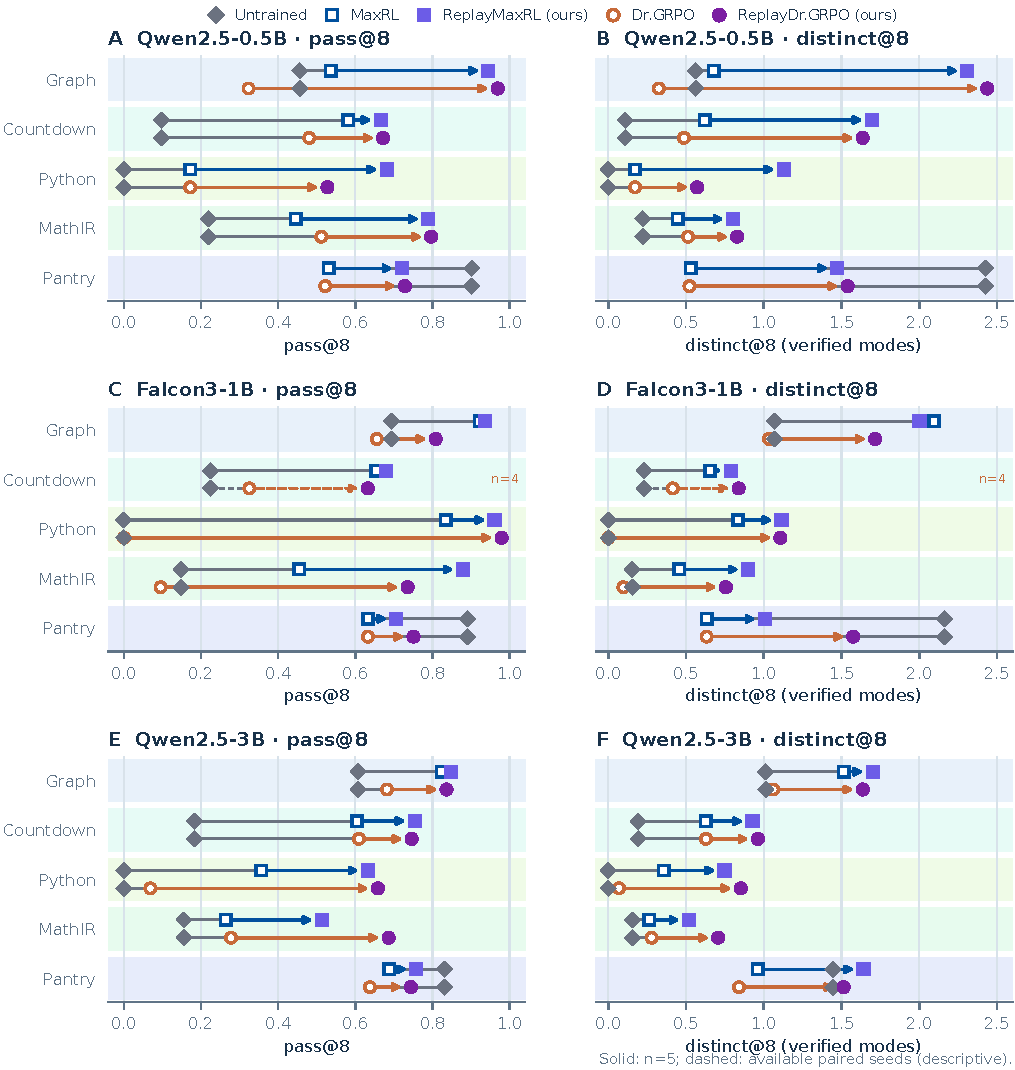
\includegraphics[width=.98\linewidth]
    {figures/e118_scale_extensions_appendix.pdf}
  \caption{\textbf{Replay gains vary by domain and model scale.}
  Final \texttt{pass@8} and \pmd{} at three model scales. Hollow and filled
  markers denote training without and with replay; circles denote Dr.GRPO,
  squares MaxRL, and gray diamonds the model before training. Correctness
  uses five paired seeds except Falcon \texttt{Countdown} Dr.GRPO ($n=4$).
  Diversity averages each arm's eligible seeds separately, requiring at least
  30 eligible prompts per seed. Lines are solid for five control seeds and
  dashed for fewer. Seed counts may differ between arms; estimates below the
  threshold are omitted. Table~\ref{tab:cross-scale-terminal-effects} reports
  paired diversity effects using a 20-prompt threshold. Error bars are omitted.}

  \label{fig:maxrl-factorial-scale-extensions}
\end{figure}


Diversity effects in Fig.~\ref{fig:replay-factorial-effects} and
Table~\ref{tab:cross-scale-terminal-effects} use paired seeds for which
both arms have at least 20 eligible evaluation prompts. The separate-arm
means in Table~\ref{tab:core-terminal-endpoints} and
Fig.~\ref{fig:maxrl-factorial-scale-extensions} instead require 30 eligible
prompts per seed in each arm. Correctness, absolute diversity, and paired
diversity effects can therefore use different seed sets; eligible prompt
subsets can also differ between arms. Diversity-effect intervals use
Student-$t$ with $n-1$ degrees of freedom for $n\ge2$ paired seeds; single-seed
effects have no interval. Correctness and mode-count intervals require five
paired seeds. All intervals are nominal 95\% estimates, without adjustment
for multiple comparisons.

For Qwen2.5-0.5B, Re:Max increases \pmd{} by $+.439$, $+.489$, and
$+.317$ on \texttt{Graph}, \texttt{Countdown}, and \texttt{PantryPlan},
respectively; each five-seed interval excludes zero. Falcon \texttt{Graph}
has a diversity effect of $-.009$ ($[-.034,+.016]$) and a correctness
effect of $+.014$ ($[-.016,+.044]$), both inconclusive. Thus a positive
cross-domain average does not imply improvement in every domain.

For Qwen2.5-3B, the five-seed \pmd{} effects are $+.076$, $+.077$,
$+.058$, $+.006$, and $+.224$ for \texttt{Graph}, \texttt{Countdown},
\texttt{Python}, \texttt{MathIR}, and \texttt{PantryPlan}, respectively.
All diversity intervals exclude zero, although the \texttt{MathIR} effect is
small. Correctness intervals exclude zero for \texttt{Countdown},
\texttt{MathIR}, and \texttt{PantryPlan}, but include zero for \texttt{Graph}
and \texttt{Python}. Across scales, Re:Max exceeds MaxRL in mean \pmd{} in
14 of 15 measurable comparisons; Re:Dr exceeds
Dr.GRPO in 14 of 14. These counts summarize
the signs of the estimated effects, not their statistical significance.

\paragraph{Cross-domain factorial summaries.}
\label{app:factorial-numerical-detail}
Weighting all five domains equally within each paired seed, Re:Max improves
\texttt{pass@8} over MaxRL by $+.307$ at Qwen2.5-0.5B (95\% interval
$[+.208,+.406]$), $+.133$ at Falcon3-1B ($[+.043,+.223]$), and $+.154$
at Qwen2.5-3B ($[+.086,+.222]$). Each comparison uses five seeds. The
corresponding Re:Dr effects are $+.337$, $+.442$, and $+.279$. The Falcon
Dr.GRPO comparison uses four common seeds and has no interval; the other
two use five.

At Qwen2.5-3B, MaxRL and Re:Max have mean correctness $.547$ and $.701$,
and mean \distk{} $.744$ and $1.107$, respectively. Their paired mode-count
difference is $+.363$ ($[+.285,+.441]$). The cross-domain \pmd{} means in
Table~\ref{tab:cross-scale-terminal-effects} use a fixed set of domains
eligible for every contributing seed.

\subsection{Level 1 at Qwen2.5-7B}
\label{app:qwen7b-level1}

We also compare MaxRL and Re:Max at Qwen2.5-7B on Level~1 in
3 domains. The 6 training runs form one
matched treatment--control pair per domain, each trained for
3072 updates with the same prompts, horizon, verifier,
evaluation procedure, and replay schedule as the smaller-scale comparisons.
With one matched seed per domain, these effects are descriptive and have no
confidence intervals.

On \texttt{MathIR}, MaxRL's observed \texttt{pass@8} reaches zero
at update 960 and remains zero at subsequent evaluations.
The final evaluation contains no verified response, so \pmd{} cannot be
estimated. Table~\ref{tab:qwen7b-level1} reports it as undefined rather than
zero. Re:Max, evaluated on the same prompts and seed, reaches
.744 \texttt{pass@8} and .017
\pmd{}. The correctness result remains measurable even though a paired
diversity effect is unavailable.

Where both conditions have measurable diversity, Re:Max increases \pmd{}
by +.298 on \texttt{Graph} and
+.137 on \texttt{Countdown}. These point estimates
exceed the corresponding 3B means, but one seed does not establish a trend
with model scale. Mean \texttt{pass@8} across all 3 domains
is .342 for MaxRL and .789 for Re:Max. Mean
\pmd{} is .028 and .245, respectively, over the
2 domains where both conditions define it. Thus the
correctness mean includes \texttt{MathIR}, while the diversity
mean does not.

\begin{table}[!htbp]
  \centering
  \caption{\textbf{Level-1 correctness and solution diversity at Qwen2.5-7B.}
  Results from 6 runs with 1 matched seed per
  domain after 3072 updates. On \texttt{MathIR},
  MaxRL produces no verified response: its correctness is zero, while its
  \pmd{} and the paired diversity effect are undefined (\texttt{--}).
  Means use 3 domains for correctness and the
  2 jointly eligible domains for diversity. No confidence
  intervals are reported per domain for these single-seed comparisons.}

  \label{tab:qwen7b-level1}
  \small
  \setlength{\tabcolsep}{6pt}
  \begin{tabular}{@{}l*{6}{r}@{}}
    \toprule
    & \multicolumn{2}{c}{\textbf{MaxRL}} & \multicolumn{2}{c}{\textbf{Re:Max}}
      & \multicolumn{2}{c}{\textbf{Re:Max $-$ MaxRL}} \\
    \cmidrule(lr){2-3}\cmidrule(lr){4-5}\cmidrule(lr){6-7}
    \textbf{Domain} & \texttt{pass@8} & \pmd{} & \texttt{pass@8} & \pmd{}
      & \texttt{pass@8} & \pmd{} \\
    \midrule
    % Generated by ops/build_paper_e124_qwen7b_level1.py; do not hand edit.
  \texttt{Countdown} & .631 & .001 & .805 & .138 & +.174 & +.137 \\
  \texttt{Graph} & .396 & .055 & .818 & .353 & +.422 & +.298 \\
  \texttt{MathIR} & .000 & -- & .744 & .017 & +.744 & -- \\
  \midrule
  Mean & .342 & .028 & .789 & .245 & +.447 & +.217 \\
  \bottomrule

  \end{tabular}
\end{table}

\subsection{Results on harder benchmark levels}
\label{app:level2-interim}

\begin{figure}[!htbp]
\centering
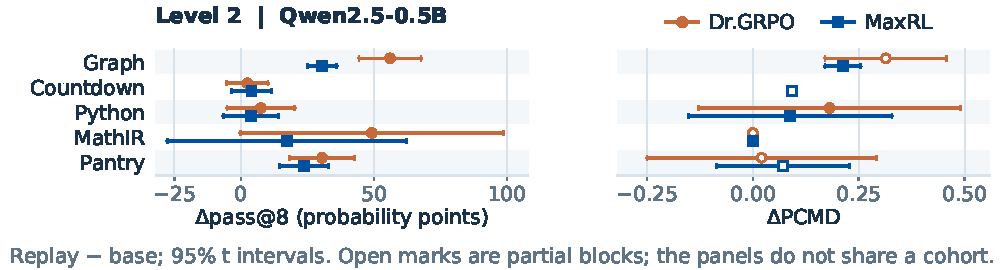
\includegraphics[width=\linewidth]{figures/replay_level2_effects.pdf}
\caption{\textbf{Replay improves Level-2 \texttt{Graph} accuracy and solution diversity.}
Final Re:Dr minus Dr.GRPO (circles) and Re:Max minus MaxRL (squares) effects
for Qwen2.5-0.5B, in percentage points of \texttt{pass@8} and \pmd{} units.
Correctness uses five paired seeds per domain. Diversity requires at least
20 eligible prompts per arm. Re:Dr uses three seeds for \texttt{Graph} and
\texttt{PantryPlan}, four for \texttt{MathIR}, and none for
\texttt{Countdown}; Re:Max uses one for \texttt{Countdown} and four for
\texttt{PantryPlan}. Other comparisons use five. Hollow markers indicate
fewer than five pairs; blanks indicate no eligible pair. Bars show nominal
paired 95\% Student-$t$ intervals for comparisons with at least two seeds.}

  \label{fig:replay-level2-effects}
\end{figure}

Fig.~\ref{fig:level2-admission} compares replay effects across Levels 1--3
using fixed domain sets. Correctness gives equal weight to \texttt{Graph},
\texttt{Countdown}, \texttt{Python}, and \texttt{PantryPlan} within each of
five common training seeds. Diversity first averages eligible seeds within
each arm and domain, then weights \texttt{Graph}, \texttt{MathIR}, and
\texttt{PantryPlan} equally. Its contributing seeds can differ across arms
and levels, so differences between these diversity means are descriptive
and have no intervals. At Level 2, only \texttt{PantryPlan} has sufficient
verified responses before training to estimate diversity; the initial
three-domain diversity mean is therefore undefined.

Each Level-2 method has five final training seeds per domain. The diversity
comparisons in Fig.~\ref{fig:replay-level2-effects} additionally require
eligible prompts in both arms. \texttt{Graph} improves under both objectives:
Re:Max increases \pmd{} by $+.212$ ($[+.170,+.255]$, five seeds), and
Re:Dr by $+.314$ ($[+.170,+.458]$, three seeds). The corresponding
\texttt{Python} effects are $+.088$ and $+.181$, with intervals including
zero; \texttt{MathIR} effects are near zero. \texttt{PantryPlan}
correctness improves by $+.305$ under Re:Dr and $+.237$ under Re:Max,
each measured over five seeds.

Each Level-2 \texttt{MathIR} prompt admits one shortest derivation and four
longer alternatives. Concentration on the shortest route therefore yields
near-zero diversity despite the existence of other valid modes. The levels
also use different held-out problems and can differ in mode-count
distributions and prompt guidance (App.~\ref{app:data-levels}). Cross-level
comparisons consequently do not isolate the causal effect of difficulty.

For each common seed and endpoint $Y$, the replay interaction is
\[
 I=(Y^{\rm Re:Max}-Y^{\rm MaxRL})
    -(Y^{\rm Re:Dr}-Y^{\rm Dr.GRPO}).
\]
A negative interaction means that replay adds less under MaxRL than under
Dr.GRPO; it does not imply that replay harms MaxRL. On Level-2
\texttt{Graph}, MaxRL alone improves \texttt{pass@8} over Dr.GRPO by
$+.233$ ($[+.140,+.325]$), while the replay interaction is $-.256$
($[-.329,-.183]$). Replay improves both objectives, with a smaller
additional benefit under the stronger fresh objective.

\begin{table}[!htbp]
  \centering
  \caption{\textbf{A stronger fresh objective need not increase the additional benefit of replay.}
  Contrasts use five common seeds per domain across all four methods.
  The interaction is
  $(\mathrm{Re:Max}-\mathrm{MaxRL})-(\mathrm{Re:Dr}-\mathrm{Dr.GRPO})$.
  Here $P_8=\texttt{pass@8}$, $D_8=\texttt{distinct@8}$, and $B_8=D_8-P_8$.
  Entries report paired means and nominal 95\% Student-$t$ intervals. Both
  mode-count metrics depend on correctness. The conditional-diversity analysis
  in Fig.~\ref{fig:replay-level2-effects} applies separate eligibility
  requirements, so its seed populations can differ from those in this table.}

\label{tab:level2-factorial-contrasts}
  \scriptsize
  \setlength{\tabcolsep}{3pt}
  \resizebox{\linewidth}{!}{%
  \begin{tabular}{@{}lclrrr@{}}
    \toprule
    \textbf{Domain} & $n$ & \textbf{Contrast} &
    $\Delta P_8$ & $\Delta D_8$ & $\Delta B_8$ \\
    \midrule
    % Domain & paired n & contrast & delta pass@8 & delta distinct@8 & delta extra modes
Graph & 5 & MaxRL $-$ Dr.GRPO & $+.233\;[+.140,+.325]$ & $+.322\;[+.162,+.482]$ & $+.089\;[+.019,+.159]$ \\
Graph & 5 & Re:Max $-$ Re:Dr & $-.023\;[-.062,+.016]$ & $-.029\;[-.198,+.140]$ & $-.006\;[-.142,+.130]$ \\
Graph & 5 & Replay $\times$ MaxRL interaction & $-.256\;[-.329,-.183]$ & $-.351\;[-.446,-.255]$ & $-.095\;[-.186,-.003]$ \\
Countdown & 5 & MaxRL $-$ Dr.GRPO & $-.014\;[-.073,+.045]$ & $-.014\;[-.073,+.045]$ & $+.000\;[+.000,+.000]$ \\
Countdown & 5 & Re:Max $-$ Re:Dr & $+.002\;[-.008,+.012]$ & $-.002\;[-.047,+.044]$ & $-.004\;[-.042,+.035]$ \\
Countdown & 5 & Replay $\times$ MaxRL interaction & $+.016\;[-.047,+.078]$ & $+.012\;[-.068,+.092]$ & $-.004\;[-.042,+.035]$ \\
Python & 5 & MaxRL $-$ Dr.GRPO & $+.000\;[+.000,+.000]$ & $+.000\;[+.000,+.000]$ & $+.000\;[+.000,+.000]$ \\
Python & 5 & Re:Max $-$ Re:Dr & $-.037\;[-.232,+.157]$ & $-.188\;[-.988,+.613]$ & $-.150\;[-1.014,+.713]$ \\
Python & 5 & Replay $\times$ MaxRL interaction & $-.037\;[-.232,+.157]$ & $-.188\;[-.988,+.613]$ & $-.150\;[-1.014,+.713]$ \\
MathIR & 5 & MaxRL $-$ Dr.GRPO & $+.283\;[-.193,+.759]$ & $+.283\;[-.193,+.759]$ & $+.000\;[+.000,+.000]$ \\
MathIR & 5 & Re:Max $-$ Re:Dr & $-.036\;[-.158,+.085]$ & $-.035\;[-.158,+.088]$ & $+.002\;[-.003,+.006]$ \\
MathIR & 5 & Replay $\times$ MaxRL interaction & $-.320\;[-.864,+.225]$ & $-.318\;[-.860,+.224]$ & $+.002\;[-.003,+.006]$ \\
PantryPlan & 5 & MaxRL $-$ Dr.GRPO & $+.019\;[-.067,+.105]$ & $+.019\;[-.081,+.119]$ & $+.000\;[-.021,+.021]$ \\
PantryPlan & 5 & Re:Max $-$ Re:Dr & $-.049\;[-.113,+.014]$ & $-.061\;[-.249,+.128]$ & $-.012\;[-.145,+.122]$ \\
PantryPlan & 5 & Replay $\times$ MaxRL interaction & $-.068\;[-.168,+.032]$ & $-.080\;[-.279,+.119]$ & $-.012\;[-.134,+.110]$ \\
    \bottomrule

  \end{tabular}}
\end{table}


\paragraph{Level-2 \texttt{Graph} results.}
\label{app:levels-numerical-detail}
Before training, Qwen2.5-0.5B \texttt{Graph} \texttt{pass@8} is $.438$
on the Level-1 development split and $.148$ on Level 2. After eight Level-2
training passes, Dr.GRPO and MaxRL reach $.202$ and $.434$, compared
with $.763$ and $.739$ for Re:Dr and Re:Max. The paired correctness gains
are $+.561$ and $+.305$, with 95\% Student-$t$ intervals $[+.445,+.677]$
and $[+.250,+.360]$ over five seeds each. The lowest replay accuracy
($.711$) exceeds the highest accuracy without replay ($.477$). Replay adds
$1.019$ and $.668$ distinct verified modes for the two objectives,
respectively, yielding \texttt{distinct@8} of $1.243$ and $1.214$.

For the three eligible Dr.GRPO seed pairs, \pmd{} rises from $.039$ to
$.353$; for the five MaxRL pairs, it rises from $.112$ to $.325$.
Expressed on the effective-mode scale, these changes are $1.04$ to $1.55$
and $1.13$ to $1.48$, corresponding to ratios of $1.49$ and $1.32$.
Relative increases in \pmd{} are unstable near a zero baseline, so we
report absolute changes instead. The joint improvements in correctness and
diversity do not establish that greater diversity causes better correctness.

\subsection{Accuracy and verified modes throughout training}
\label{app:factorial-training-curves}

Figs.~\ref{fig:factorial-training-accuracy}--\ref{fig:level2-training-pmd}
show correctness and diversity throughout training, using four groups of
eight responses to each of 128 held-out prompts. Lines show seed means;
bands show the range across seeds, rather than confidence intervals. A seed
contributes to conditional diversity only when at least five prompts have
two or more correct responses. The contributing seeds and prompts can
therefore change across methods and checkpoints.

\begin{figure}[!htbp]
  \centering
  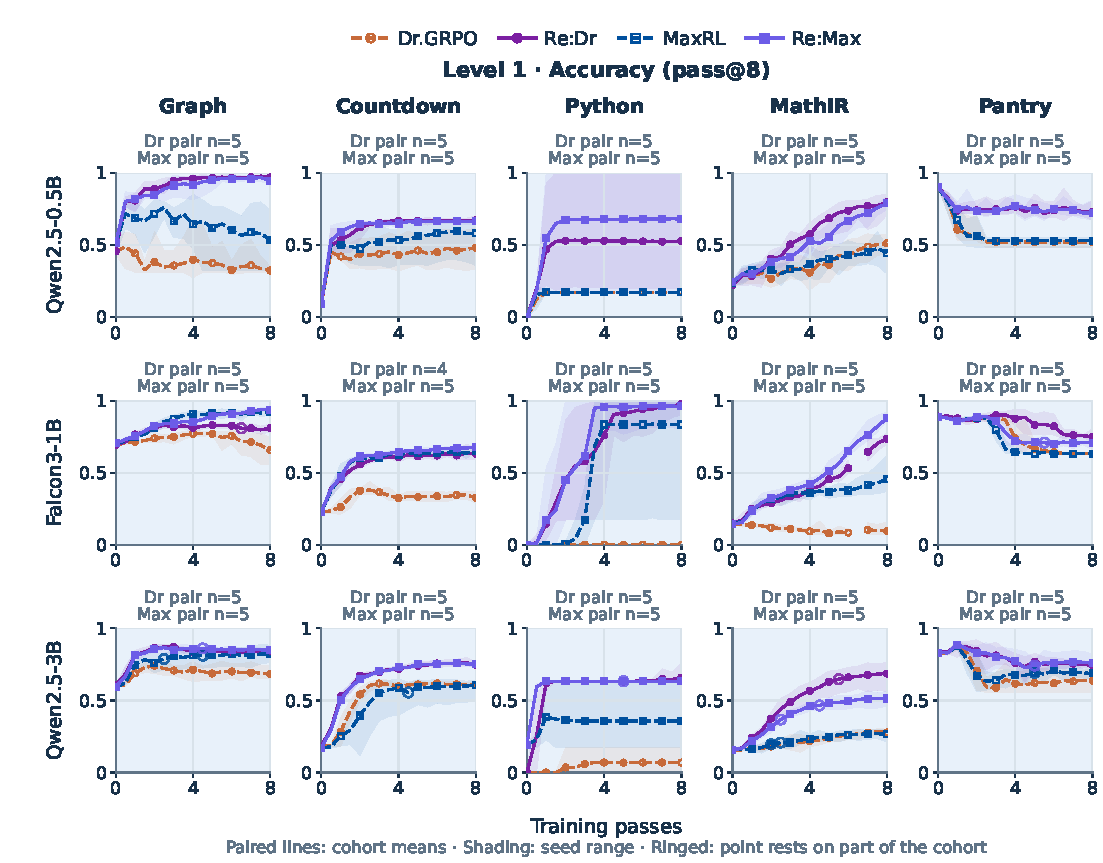
\includegraphics[width=\linewidth]{figures/factorial_training_curves_pass8.pdf}
  \caption{\textbf{Replay improves final accuracy across model scales.}
  \texttt{pass@8} over eight training passes for Dr.GRPO, Re:Dr, MaxRL, and
  Re:Max. Rows show Qwen2.5-0.5B, Falcon3-1B, and Qwen2.5-3B; columns show
  domains. Panel labels give the numbers of paired seeds at the final
  checkpoint. Lines show seed means and bands show seed ranges, rather than
  confidence intervals. Ringed points use fewer seeds than the final comparison.}

  \label{fig:factorial-training-accuracy}
\end{figure}

\begin{figure}[!htbp]
  \centering
  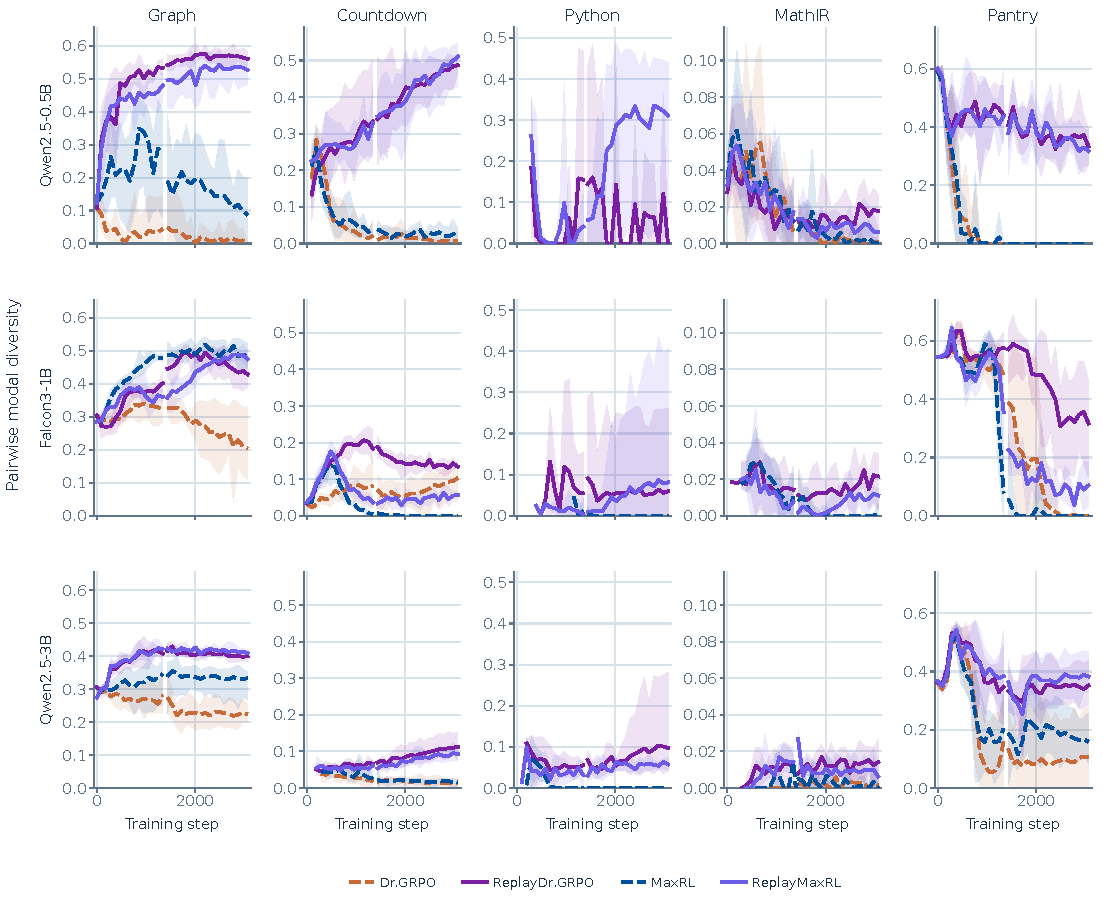
\includegraphics[width=\linewidth]{figures/factorial_training_curves_pmd.pdf}
  \caption{\textbf{Replay limits the loss of \texttt{PantryPlan} solution diversity at every scale.}
\pmd{} throughout training, with model rows and method colours as in
Fig.~\ref{fig:factorial-training-accuracy}. Both fresh objectives reach zero
terminal \texttt{PantryPlan} diversity at 0.5B and 1B, whereas both replay variants
retain multiple solution modes. Lines average one to five eligible seeds
per checkpoint; bands show seed ranges and are absent for a single seed.
A seed contributes when at least five prompts yield at least two correct responses.
Fine dotted segments use fewer seeds, so changes can reflect sample
composition. Gaps indicate undefined estimates. Vertical scales are shared
within each domain.}
  \label{fig:factorial-training-modes}
\end{figure}

\begin{figure}[!htbp]
  \centering
  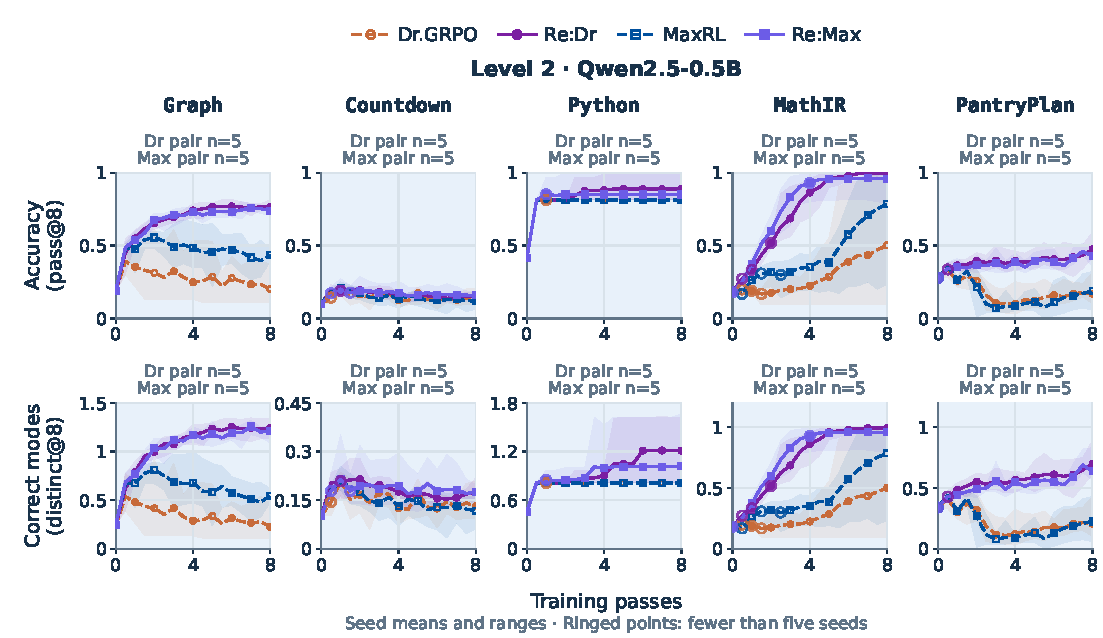
\includegraphics[width=\linewidth]{figures/level2_factorial_training_curves.pdf}
  \caption{\textbf{Replay improves final accuracy and verified-mode counts at Level~2.}
Qwen2.5-0.5B trajectories for Dr.GRPO, Re:Dr, MaxRL, and Re:Max across five
domains. Rows show \texttt{pass@8} and \distk{}; the latter depends on both
correctness and solution diversity. Each objective pair has five matched
seeds at the terminal checkpoint. Lines show seed means and bands show
seed ranges. Ringed points use fewer than five seeds; Fig.~\ref{fig:level2-training-pmd}
reports success-conditional diversity.}
  \label{fig:level2-training-curves}
\end{figure}

\begin{figure}[!htbp]
  \centering
  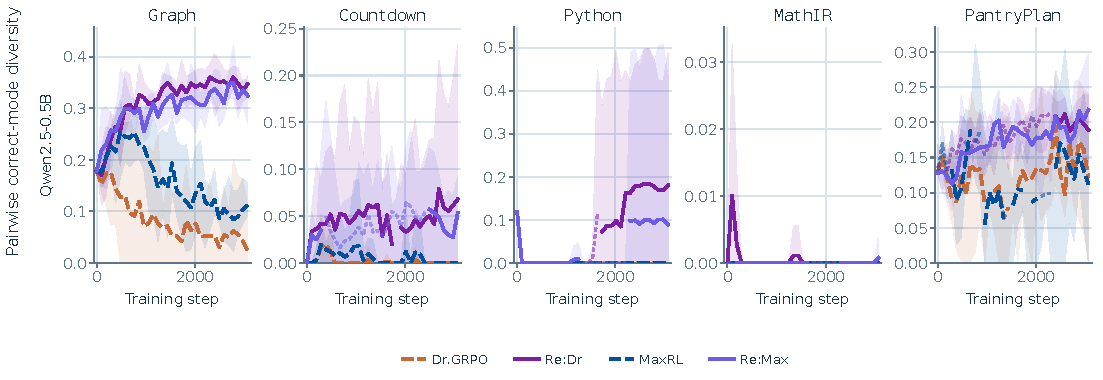
\includegraphics[width=\linewidth]{figures/level2_training_curves_pmd.pdf}
  \caption{\textbf{Replay preserves greater solution diversity on Level-2 \texttt{Graph}.}
\pmd{} during Qwen2.5-0.5B training for the four primary methods. At the
terminal checkpoint, Re:Dr and Re:Max reach $.346$ and $.325$, compared with
$.023$ for Dr.GRPO and $.112$ for MaxRL. \texttt{MathIR} remains near zero under all
four methods. Lines average eligible seeds and bands show seed ranges.
Each seed requires at least five prompts with at least two correct responses.
Fine dotted segments indicate fewer contributing seeds, and gaps indicate that the estimate is undefined.}
  \label{fig:level2-training-pmd}
\end{figure}


\subsection{Supporting comparators}
\label{app:ucpo-progress}

GRPO normalizes rewards within each group; UCPO redistributes the advantage
among fresh on-policy responses; sparse RLEP-Dr reuses verified successes
without uniform weighting by canonical key. We evaluate GRPO in 75 training
runs across three model scales. UCPO and RLEP-Dr cover the two smaller
scales, with 50 and 47 runs, respectively. RLEP-Dr uses two seeds for Falcon
\texttt{Python} and five elsewhere. Fixed Semantic-MaxEnt adds a
frequency-based bonus to fresh responses (App.~\ref{app:semantic-maxent}).
Its four-method factorial covers ten model--domain combinations at the two
smaller scales, with five common seeds except Falcon \texttt{Countdown}
($n=4$). The 3B comparison uses one seed to evaluate adding the bonus to
replay (App.~\ref{app:semantic-current-factorial}).

For GRPO, UCPO, and RLEP-Dr, the diversity contrasts in this subsection
average per-prompt differences over prompts with at least two correct
responses in both arms. Each seed must have at least 30 such jointly
eligible prompts. Table~\ref{tab:direct-comparator-matrix} instead uses
separate 20-prompt thresholds for each arm. On Qwen2.5-0.5B \texttt{Graph},
one UCPO seed and four RLEP-Dr seeds meet the joint criterion; no
\texttt{Python} comparison meets it at any scale.

For Qwen2.5-0.5B, UCPO improves \texttt{Countdown} \texttt{pass@8} by
$+.133$ ($[+.005,+.262]$), while its \pmd{} effect is inconclusive:
$+.002$ ($[-.018,+.023]$). Its \texttt{MathIR} effects are also
inconclusive. RLEP-Dr improves \texttt{MathIR} correctness by $+.126$
($[+.030,+.222]$), with zero measured diversity change; its
\texttt{Countdown} and Falcon \texttt{PantryPlan} effects are inconclusive.
Across GRPO, UCPO, and RLEP-Dr, seven of 34 five-seed correctness intervals
lie above zero. None of the 19 five-seed diversity intervals lies above zero; one lies
below zero, for Falcon \texttt{Countdown} GRPO: $-.105$
($[-.147,-.063]$). At Qwen2.5-3B, all five GRPO correctness intervals and
the three available diversity intervals include zero. These are nominal
paired 95\% Student-$t$ intervals over training seeds.

The uniform versus frequency-weighted replay comparison uses five paired
seeds in each of nine model--domain combinations: all five Qwen2.5-0.5B
domains, plus \texttt{Graph} and \texttt{PantryPlan} at both larger scales.
Changing only the within-buffer weights increases extra verified modes by
$+.318$ per prompt in the Qwen2.5-0.5B average ($[+.272,+.358]$,
paired-seed bootstrap). The correctness effect is inconclusive at $+.010$
($[-.119,+.139]$). This result supports a benefit from uniform weighting
beyond reusing successful responses in proportion to their frequency,
although extra-mode counts still depend on correctness
(App.~\ref{app:frequency-replay-progress}).

RLEP-Dr's offline response pool uses temperature $.7$ and top-$p=.95$;
evaluation uses temperature 1 and top-$p=1$. Its offline data collection
also differs from the online construction of prompt-specific verified replay
buffers, and the next paragraph measures what that difference puts in the pool.

\paragraph{What RLEP-Dr replays.}
\phantomsection\label{app:rlep-pool}
RLEP's protocol harvests its experience pool from a policy that RL has
already trained \citep{zhang2025rlep}: the seed policy samples 64 candidates
per prompt at temperature $.7$ and top-$p=.95$, verified answers are kept, and
a prompt enters the pool only with at least two of them. Here the seed policy
is the paired terminal Dr.GRPO control, so the pool is a sample from the
collapsed endpoint that Sec.~\ref{sec:results-collapse} measures.
Table~\ref{tab:rlep-pool-composition} reads the frozen pools and the learner
telemetry of every RLEP-Dr cell. At Qwen2.5-0.5B,
43\%--79\% of the 384 training prompts hold
no verified trajectory and never receive a replay row. Of the
4393 eligible prompts pooled over all 25
cells, all but 17 hold a single canonical key among
their verified trajectories, and none holds more than 2, so a
two-row replay draw is two copies of one mode with probability at least
.99 in every domain.
Falcon3-1B pools are slightly wider on \texttt{Graph} and \texttt{Countdown},
up to 1.40 keys per eligible prompt, and a same-mode pair
remains the draw with probability
.89--1.00. The online Re:Dr buffer on the
same prompts and seeds holds 2.6--6.9 modes on average
in the three domains where modes are plentiful. RLEP-Dr's replay is therefore
single-mode replay of the control's own endpoint, applied on
21\%--57\% of updates, and its \pmd{} beside the
control is the expected outcome rather than a discrepancy with Re:Dr: no
update rule rehearses a second mode from a pool that holds one.

The two update rules are closer than their descriptions suggest. RLEP's
replay row enters the policy gradient with advantage $1-\bar r$, where
$\bar r$ is the mean reward of the mixed group, so it is a positive-coefficient
log-likelihood term on a stored success, as Re:Dr's replay term is. The
difference is that RLEP's coefficient shrinks toward zero as the prompt is
solved, with a realized mean of .03--.38 across domains
at 0.5B, whereas Re:Dr's is fixed. Whether a likelihood term on a single
stored success can produce breadth is tested directly by the capacity-one arm
of App.~\ref{app:mode-agnostic-replay}, which applies exactly such a term to
one success captured online at first discovery and recovers 58\% of
the Re:Dr effect. What separates the two replay families is thus not the loss
but the buffer: what it stores, from which policy, and from when.

\begin{table}[H]
  \centering
  \caption{\textbf{RLEP-Dr's pools hold one mode per prompt.} Composition of
  the frozen RLEP experience pools and the realized replay dose, averaged over
  seeds. \emph{none} is the share of the 384 training prompts with no verified
  trajectory; \emph{eligible} the share with at least two; \emph{keys} the mean
  number of canonical modes among an eligible prompt's verified trajectories;
  $P(\text{same})$ the probability that a two-row replay draw repeats one
  mode; \emph{updates} the share of optimizer updates that mixed in replay
  rows; $A_{\text{replay}}$ the mean replay advantage $1-\bar r$ on those
  updates. The last column is the mean number of modes in the Re:Dr buffer
  over the within-cohort cells on the same prompts and seeds
  (Tab.~\ref{tab:matched-redr}).}
  \label{tab:rlep-pool-composition}
  \small
  \setlength{\tabcolsep}{5pt}
  \begin{tabular}{@{}lrrrrrrrr@{}}
    \toprule
    \textbf{Domain} & $n$ & \textbf{none} & \textbf{eligible} & \textbf{keys}
      & $P(\text{same})$ & \textbf{updates} & $A_{\text{replay}}$
      & \textbf{Re:Dr modes} \\
    \midrule
    % Generated by ops/build_paper_rlep_pool_composition.py; do not hand edit.
  \multicolumn{9}{@{}l}{\textit{Qwen2.5-0.5B}} \\
  \texttt{Graph} & 5 & 64\% & 36\% & 1.00 & 1.00 & 36\% & .19 & 3.77 \\
  \texttt{Countdown} & 5 & 43\% & 57\% & 1.02 & .99 & 57\% & .11 & 2.56 \\
  \texttt{Python} & 5 & 79\% & 21\% & 1.00 & 1.00 & 21\% & .03 & 1.20 \\
  \texttt{MathIR} & 5 & 43\% & 57\% & 1.00 & 1.00 & 57\% & .38 & 1.15 \\
  \texttt{PantryPlan} & 5 & 43\% & 57\% & 1.00 & 1.00 & 57\% & .03 & 6.88 \\
  \multicolumn{9}{@{}l}{\textit{Falcon3-1B}} \\
  \texttt{Graph} & 5 & 44\% & 56\% & 1.40 & .89 & 56\% & .41 & \textemdash{} \\
  \texttt{Countdown} & 5 & 56\% & 44\% & 1.17 & .95 & 44\% & .24 & \textemdash{} \\
  \texttt{Python} & 2 & 90\% & 10\% & 1.01 & 1.00 & 10\% & .50 & \textemdash{} \\
  \texttt{MathIR} & 5 & 91\% & 9\% & 1.01 & 1.00 & 9\% & .30 & \textemdash{} \\
  \texttt{PantryPlan} & 5 & 41\% & 59\% & 1.00 & 1.00 & 59\% & .09 & \textemdash{} \\
  \bottomrule

  \end{tabular}
\end{table}

\paragraph{Comparator settings.}
\phantomsection\label{app:comparator-settings}
Each comparator shares the non-objective settings of its paired control
(Table~\ref{tab:run-contract}). UCPO uses the published default
$\omega=.2$, and RLEP-Dr uses the published combination of 16 fresh and
2 replay responses. GAPO has no free coefficient; its reward is affinely
mapped to the control's unit range because Dr.GRPO does not normalize by
the group standard deviation. SetPO uses $\lambda=1.0$, giving a diversity
term approximately 5.3\% of the task advantage; its paper provides no
coefficient for the 0.5B verifier-reward setting. Semantic-MaxEnt uses
$\eta=.10$ and $\kappa=5$. Replay uses $\lambda_{\mathrm{replay}}=.10$
and capacity $M=16$, equal to the rollout group size. These settings are
not tuned to \mb{} outcomes, and no method receives a learning-rate sweep.
The results therefore compare the methods at the stated settings;
hyperparameter tuning could improve correctness or diversity.

\paragraph{Interpreting zero diversity.}
In Table~\ref{tab:direct-comparator-matrix}, an em-dash denotes an undefined
paired difference. An exact $.000$ instead denotes a measured zero, with
identical values for both methods in every eligible seed. The
\texttt{Python} \pmd{} column contains measured zeros because, for each
eligible prompt, both methods' verified responses share a single execution
key. High correctness can coexist with this concentration: four of the five
SetPO \texttt{Python} seeds reach \texttt{pass@8} $1.000$ and terminal
\pmd{} $.000$. Every held-out prompt has at least one correct response,
but the verified responses for each prompt use a single mode. Per-response
correctness also increases in all 15 control comparisons
(App.~\ref{app:control-learning-audit}).

\begin{figure}[!htbp]
  \centering
  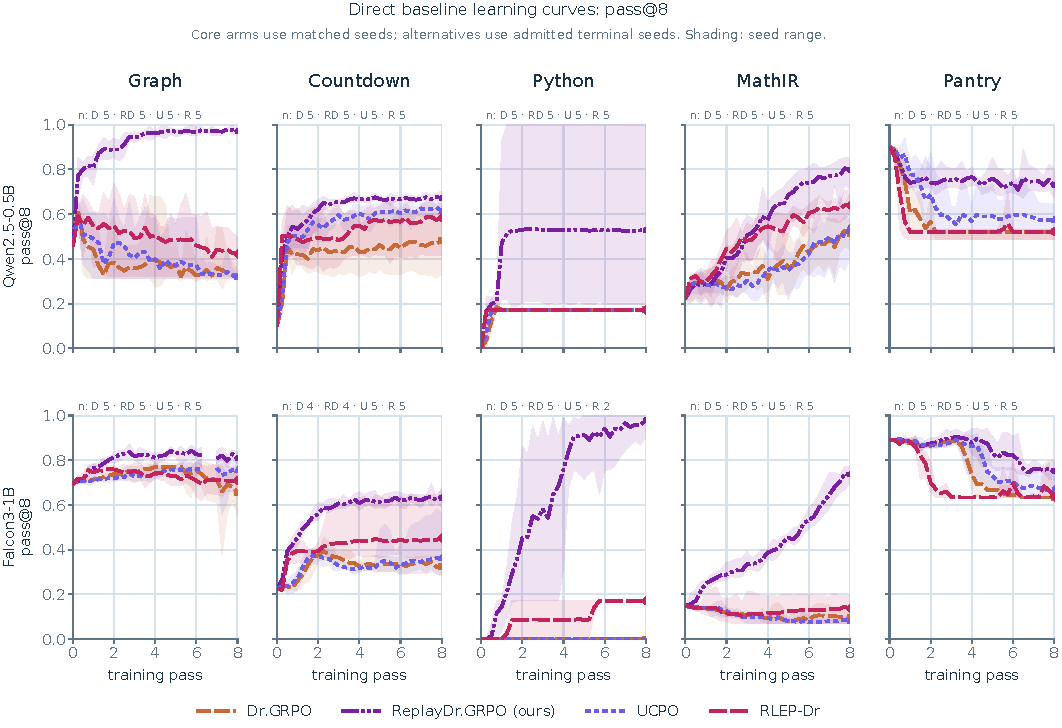
\includegraphics[width=\linewidth]{figures/direct_baseline_learning_curves_pass8.pdf}
  \caption{\textbf{Re:Dr has the highest terminal mean accuracy in every
  displayed comparison.} \texttt{pass@8} during Level-1 training for Dr.GRPO,
  Re:Dr, UCPO, and sparse RLEP-Dr. Rows show Qwen2.5-0.5B and Falcon3-1B;
  columns show the five domains. Lines show seed means and bands show seed
  ranges; gaps indicate unavailable estimates. Dr.GRPO and Re:Dr use paired
  seeds. Comparisons use five seeds except Falcon \texttt{Countdown}
  Dr.GRPO/Re:Dr ($n=4$) and Falcon \texttt{Python} RLEP-Dr ($n=2$), as indicated in the panels.}
  \label{fig:direct-baseline-accuracy-curves}
\end{figure}


\subsection{Diversity-preserving comparators}
\label{app:diversity-comparators}

GAPO~\citep{anschel2025groupaware} and SetPO~\citep{li2026setpo} target
output diversity within the fresh rollout group. Both are evaluated on
Level-1 Qwen2.5-0.5B across five domains and five seeds. GAPO assigns
verifier-positive rollouts the reward $[1-(f_i-1/L)+1]/2$, with zero for
failures, where $f_i$ is the key's frequency among the group's verified
rollouts and $L$ is the prompt's certified number of valid modes.
SetPO augments each rollout's advantage by its marginal contribution to
kernelized set diversity, measured by removing that rollout from the group,
with coefficient $\lambda=1$. It computes similarities using a fixed
\texttt{all-MiniLM-L6-v2} sentence encoder, mean pooling, and cosine
similarity clamped to $[0,1]$. Encoding the responses adds computation.

GAPO increases \pmd{} on \texttt{Countdown} ($+.340$, $[+.112,+.567]$) and \texttt{PantryPlan}
($+.653$, $[+.610,+.696]$), while its \texttt{Python} effect is near zero
with an interval spanning zero. \texttt{Python} has more valid modes than the
sixteen-rollout group can represent on 95\% of training prompts, with up to 3,600
modes. This limits within-group coverage but does not prevent a policy from
assigning mass across the full support. \texttt{MathIR} effects are small across
methods; the largest is Re:Dr's $+.017$ ($[+.003,+.031]$).
SetPO increases \pmd{} on \texttt{PantryPlan} ($+.266$, $[+.177,+.356]$); its other
four domain intervals include zero. Five-domain mean effects are $+.225$
for GAPO, $+.066$ for SetPO, and $+.320$ for Re:Max, although GAPO's
\texttt{PantryPlan} effect is larger than Re:Max's. The effective number
of modes, $\neff$, on \texttt{PantryPlan} is $2.88$ for GAPO and $1.36$
for SetPO, compared with $1.00$ for their shared control. SetPO also raises
\texttt{Python} \texttt{pass@8} from $.338$ to $.834$, a relative increase
of $147\%$. Relative changes in \pmd{} are undefined for \texttt{PantryPlan}
and \texttt{Python} because the control has $\pmd=.000$. GAPO adjusts
rewards using frequencies within the fresh rollout group, whereas replay
balances the likelihood term across verified modes accumulated in the buffer.

GAPO and SetPO share a Dr.GRPO control with matching hardware and
nonoverlapping evaluation draws. Its terminal \pmd{} differs from the
Dr.GRPO control used in the main replay comparison by a mean of $+.003$
over twenty paired comparisons, ranging from $-.014$ to $+.034$. These
observed differences are small relative to the five-domain effects above,
but do not establish equivalence between the controls.

\subsection{Measured KL tradeoffs and replay occupancy}
\label{app:kl-measured}

Table~\ref{tab:reference-kl-measured} compares terminal \pmd{} at
Qwen2.5-0.5B, Level~1, after $3{,}072$ updates. Dr.GRPO with reference KL
uses 6 coefficients, $\beta\in\{0.001, 0.01, 0.04, 0.1, 0.2, 0.3\}$, across
5 domains. These arms use the zero-replay-derivative control
configuration with a nonzero KL coefficient and the initial policy as the
reference. The comparisons match optimizer updates and fresh-rollout
budgets. They do not equalize total computation: reference-policy evaluation
and replay processing incur different costs, and the control does not spend
those costs on additional effective updates or fresh rollouts.

\begin{figure}[t]
  \centering
  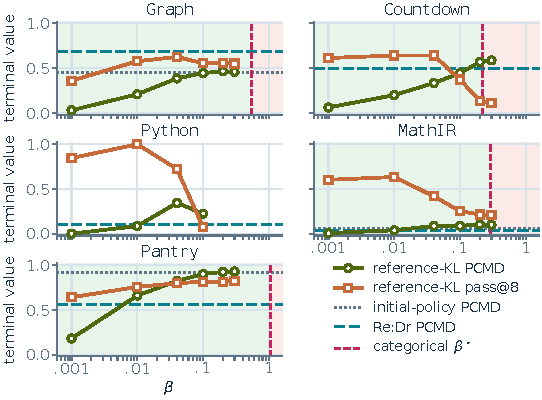
\includegraphics[width=0.78\linewidth]{figures/reference_kl_knee.pdf}
  \caption{\textbf{KL coefficient effects vary by domain.}
  Circles show terminal \pmd{} and squares show \texttt{pass@8} for
  Qwen2.5-0.5B at Level~1; lines connect seed means without uncertainty
  bands. Horizontal rules mark the initial policy's reportable \pmd{}
  (dotted) and Re:Dr's terminal \pmd{} (dashed). Vertical rules mark the
  categorical plug-in threshold $\beta^\star$; green and red indicate
  stationary single-draw correctness above and below one half under that
  calculation. This threshold does not predict the location of the observed
  \texttt{pass@8} knee.}
  \label{fig:reference-kl-knee}
\end{figure}

\paragraph{Initial concentration and coefficient dependence.}
Dr.GRPO without KL reaches \pmd{} at or below $.004$ in all five domains.
MaxRL without replay reaches $.148$ in \texttt{Graph} and at or below $.022$
elsewhere. These low values are consistent with concentration, but the
neural runs do not satisfy the independent-logit assumptions of
Proposition~\ref{thm:grpo-collapse}.
KL produces larger conditional-diversity estimates at several coefficients
in every domain. The response is not uniformly monotone: \texttt{Graph} changes
from $.465$ to $.458$ and \texttt{MathIR} from $.103$ to $.099$ between
$\beta=.2$ and $.3$, while \texttt{Python} changes from $.344$ to $.225$ between
$\beta=.04$ and $.1$.
These are comparisons of point estimates, without a seed-level uncertainty
analysis for their differences.

\begin{table}[t]
  \centering
  \caption{\textbf{KL and replay have different domain-level tradeoffs.}
  Terminal \pmd{} seed means for Qwen2.5-0.5B, Level~1. Superscripts give
  counts below five seeds; dashes indicate unavailable cells. The four
  zero-KL arms use 32 disjoint evaluation streams; KL arms use their own
  disjoint draws with the same estimator. Reference summaries are
  initial-policy \pmd{} and $1-1/\bar k$ for each replay arm, where $\bar k$
  is the mean number of keys replayed per measured update. These do not bound
  neural diversity. The final column computes categorical $\beta^\star$
  from mean initial single-draw correctness.}
  \label{tab:reference-kl-measured}
  \scriptsize
  \setlength{\tabcolsep}{2.5pt}
  \begin{tabular}{@{}lrrrrrrrrrrrrrr@{}}
    \toprule
    & \multicolumn{2}{c}{\textbf{without replay}}
      & \multicolumn{6}{c}{\textbf{$+$ reference KL, by $\beta$}}
      & \multicolumn{2}{c}{\textbf{$+$ replay}}
      & \multicolumn{3}{c}{\textbf{reference summaries}} & \\
    \cmidrule(lr){2-3}\cmidrule(lr){4-9}\cmidrule(lr){10-11}\cmidrule(lr){12-14}
    \textbf{Domain} & Dr.GRPO & MaxRL
      & $.001$ & $.01$ & $.04$ & $.1$ & $.2$ & $.3$
      & \textbf{Re:Dr} & \textbf{Re:Max}
      & Initial & Re:Dr & Re:Max & $\beta^\star$ \\
    \midrule
    % Generated by ops/build_reference_kl_comparison.py; do not hand edit.
  \texttt{Graph}  &  0.003  &  0.148  &  0.029  &  0.207  &  0.385  &  0.444  &  0.465  &  0.458  &  0.686  &  0.625  &  0.45  &  0.75  &  0.70  &  0.55 \\
  \texttt{Countdown}  &  0.004  &  0.022  &  0.060  &  0.198  &  0.333  &  0.444  &  0.568  &  0.587  &  0.497  &  0.531  &  ---  &  0.56  &  0.52  &  0.22 \\
  \texttt{Python}  &  0.000  &  0.000  &  0.000  &  0.086  &  0.344  &  0.225$^{3}$  &  ---  &  ---  &  0.099  &  0.239  &  ---  &  0.15  &  0.42  &  --- \\
  \texttt{MathIR}  &  0.003  &  0.008  &  0.007  &  0.038  &  0.086  &  0.088  &  0.103  &  0.099  &  0.039  &  0.018  &  0.06  &  0.15  &  0.12  &  0.29 \\
  \texttt{Pantry}  &  0.000  &  0.000  &  0.180  &  0.660  &  0.824  &  0.901  &  0.925  &  0.931  &  0.557  &  0.556  &  0.91  &  0.85  &  0.85  &  1.05 \\
  \bottomrule

  \end{tabular}
\end{table}

\paragraph{Stationary predictions and measured checkpoints.}
Proposition~\ref{prop:kl-stationary} identifies the categorical interior
stationary conditional as $q^\star=\mu|_{\mathcal C}$, independently of
$\beta$. It does not bound transient diversity or establish that a finite
neural checkpoint reaches this conditional. The measured \pmd{} varies
with $\beta$ and can exceed the initial estimate: at $\beta=.2$, \texttt{Graph}
reaches $.465$ against $.454$ initially, \texttt{MathIR} $.103$ against $.061$,
and \texttt{Pantry} $.925$ against $.913$. These estimates also condition on each
policy's own verified responses, rather than on a common set of solved
prompts.

For a fixed prompt with $0<\mu(\mathcal C)<1/2$, the Dr.GRPO formula gives
\[
  \beta^\star=\frac{(G-1)/G}{-\operatorname{logit}\mu(\mathcal C)},
  \qquad P^\star(\beta^\star)=\tfrac12.
\]
The displayed values substitute each domain's mean initial correctness
and $G=16$, giving $0.22$--$1.05$.
This aggregation is descriptive: substituting a mean into the nonlinear
stationary formula does not give the mean of its promptwise predictions.
Moreover, $P^\star$ is single-draw correctness, whereas the plotted
\texttt{pass@8} measures success within eight responses. Declines in that
metric already occur below the displayed threshold: \texttt{MathIR} falls from
$.634$ at $\beta=.01$ to $.418$ at $.04$, well below its
$\beta^\star\simeq.29$. \texttt{Countdown} similarly falls from $.642$ at $.04$
to $.372$ at $.1$, below $.22$. The thresholds therefore do not locate
the measured knees. \texttt{Python} has zero observed initial successes, so no
finite plug-in threshold or reportable initial \pmd{} is shown; this
does not establish zero population correctness.

Finite training, shared parameters, prompt sampling, and the adaptive
optimizer can all separate the measured neural trajectory from the
categorical stationary calculation. The comparison does not identify their
individual effects. The boundary-force identities and the two-mode
$\Theta(1/[s\log(1/s)])$ versus $\Theta(\log(1/s))$ recovery result
characterize their stated categorical models, not measured neural recovery
rates.

\paragraph{What buffer occupancy measures.}
For a nonempty fixed uniform categorical buffer with $k$ keys, the limiting
diversity is $1-1/k$. Across such buffers,
$\E[1-1/k]\le1-1/\E[k]$ by Jensen's inequality. The table instead uses
$\bar k$, the number of keys replayed per measured update, averaged within
runs and then across seeds. Buffers change during training, and updates
without replay can contribute zero keys. Thus $1-1/\bar k$ is a
descriptive transform of training occupancy, not an estimate of the
nonempty fixed-buffer expectation in that inequality. Neither quantity
bounds held-out neural \pmd{}.

\texttt{Python} illustrates a possible discovery difference. Re:Max averages
$1.73$ replayed keys per update against Re:Dr's $1.18$, while terminal
\pmd{} is $.239$ versus $.099$. Corollary~\ref{cor:maxrl-starvation}
provides a categorical motivation for stronger fresh learning when
correctness is scarce, but these measurements do not isolate discovery
from prompt weighting, sampling, or optimization. Occupancy also does not
order all outcomes: in \texttt{Countdown}, Re:Max has fewer replayed keys per
update ($2.10$ versus $2.28$) but higher \pmd{} ($.531$ versus $.497$).
In \texttt{Pantry} both arms average about $6.7$ keys and reach about $.557$ \pmd{}.
The capacity of 16 keys would allow a uniform fixed-buffer value of
$1-1/16=.9375$; the occupancy summary near $.85$ is not that capacity
limit and does not prove why KL performs better there.

\paragraph{Observed correctness--diversity comparisons.}
In \texttt{Python} and \texttt{Pantry}, at least one measured KL coefficient exceeds both
replay arms on \pmd{} and has no lower \texttt{pass@8} point estimate.
In \texttt{Countdown} and \texttt{MathIR}, coefficients that exceed both replay arms on
\pmd{} have lower \texttt{pass@8} than both. In \texttt{Graph},
all measured coefficients are below both replay arms on both metrics.
These comparisons concern seed means; they establish neither statistical
dominance nor a ranking at equal total compute.
\paragraph{Relative and absolute readings of the Re:Max effect.}
Table~\ref{tab:reference-kl-measured} carries both arms of the Re:Max versus
Dr.GRPO comparison on one evaluation, so the effect can be read either way.
Equally weighting the five domains, Dr.GRPO reaches \texttt{pass@8} $.405$ and
Re:Max $.772$, a relative increase of $90\%$; averaging the five per-domain
relative increases instead gives $124\%$, because \texttt{Python} rises from a
small base. A relative reading of \pmd{} is not available: terminal Dr.GRPO
\pmd{} is $.000$--$.004$ across these domains and exactly $.000$ in
\texttt{Python} and \texttt{PantryPlan}, so two of the five ratios are
undefined and the rest are dominated by the denominator. The count-valued
reading is well defined instead. Re:Max reaches $\neff$ of $2.66$, $2.13$,
$1.32$, $1.02$ and $2.25$ on \texttt{Graph}, \texttt{Countdown},
\texttt{Python}, \texttt{MathIR} and \texttt{PantryPlan}, against
$1.00$--$1.004$ for Dr.GRPO: a mean ratio of $1.87$ effective verified modes
for each one the control retains. Paired per-seed \pmd{} differences on a
common eligible population, which weight prompts and seeds differently, are
reported in Table~\ref{tab:direct-comparator-matrix}.

Figure~\ref{fig:reference-kl-plane} averages \texttt{Graph}, \texttt{MathIR}, and
\texttt{Pantry}, the three domains with reportable initial \pmd{}, across all
six coefficients. Between $\beta=.2$ and $.3$, mean \pmd{} changes from
$.498$ to $.496$, while \texttt{pass@8} changes from $.527$ to $.528$.

\subsection{Reference quality, discovery, and the scope of the comparison}
\label{app:kl-case}

\paragraph{Reference quality can favor KL.}
A full-support fixed reference yields the full-support categorical
stationary policy in Proposition~\ref{prop:kl-stationary}. Reference KL
uses that policy rather than a replay buffer; it requires reference-policy
evaluation but no rule for admitting exemplars. In \texttt{Pantry} at
$\beta=0.3$, the 5-seed mean reaches
$\pmd{}=0.931$ and \texttt{pass@8} $0.825$.
The replay arm with larger \pmd{} reaches $0.557$ and
$0.797$, respectively. \texttt{Pantry}'s initial \pmd{} is
$0.91$, consistent with a useful reference conditional.
The measurements support reference quality as one possible explanation;
they do not show that replay's capacity or discovery alone causes the
difference.

\paragraph{Reference diversity varies across evaluation populations.}
App.~\ref{app:hosted-mode-diversity} reports 7
hosted deployments with macro \pmd{} spanning 0.14--0.31;
Kimi K3 is highest at 0.31. Of
101 reportable model--domain--level cells,
7 reach $.50$ and the maximum is
$0.74$. These estimates are lower than \texttt{Pantry}'s initial
$0.91$ in the local comparison, but the models,
evaluation populations, and reportability sets differ. The hosted cohort
therefore describes additional candidate reference distributions; it does
not establish how training with those references would perform. Under the
categorical proposition, each reference determines a stationary
conditional, not a ceiling on a retrained neural policy. Replay instead
targets the solution modes represented by its discovered buffer.

\paragraph{Correctness costs depend on the domain and coefficient.}
The largest observed \texttt{pass@8} reduction among KL cells that exceed
both replay arms on \pmd{} occurs in \texttt{MathIR} at
$\beta=0.3$. Its 5-seed mean is
$0.099$ \pmd{} and $0.207$ \texttt{pass@8},
compared with $0.039$ and $0.816$ for
the replay arm with larger \pmd{}. This finite-checkpoint comparison
supports a domain-dependent correctness--diversity tradeoff, without
identifying the categorical threshold as its cause.
Replay's positive dose does not change its full-coverage categorical
limit under Corollary~\ref{cor:replay-no-collapse}, only the rate at which
that limit is approached. A measured
replay-dose sweep would be needed to compare coefficient sensitivity.

\paragraph{Limits of the evidence.}
Reference \pmd{} requires at least 30 defined prompts in an initial
evaluation. This eligibility condition affects which policy conditionals
can be compared. \texttt{Python}'s zero observed initial correctness cannot
support an inheritance explanation for its measured KL gains.
\texttt{MathIR}'s support certificate counts derivations and does not imply
that a policy will produce every certified solution mode.

The categorical results separate a fixed-reference target from a
discovered-buffer target and characterize restoration under their stated
assumptions. The neural measurements compare finite checkpoints. They do
not establish a universal preference between KL and replay, a discovery
cause for every replay shortfall, or an advantage under equal total compute.

\subsection{Uniform versus fresh-frequency replay}
\label{app:frequency-replay-progress}

The weighting ablation uses the same buffer construction and update rule,
changing only the within-buffer target: uniform weights over retained keys
versus weights proportional to verifier-positive fresh-rollout counts.
The resulting policies can produce different buffer contents during training.
Positive contrasts below favor uniform weighting. We report
$B_8=\texttt{distinct@8}-\texttt{pass@8}$, extra verified modes per prompt,
and $P_8=\texttt{pass@8}$. The five-domain Qwen2.5-0.5B aggregate averages
domain effects within each matched seed, giving equal domain weight.

Paired-seed intervals enumerate all $5^5=3{,}125$ ordered bootstrap
resamples of the five paired training seeds and use linearly interpolated
2.5th and 97.5th percentiles. Each resampled seed carries its complete domain
vector for the five-domain aggregate. These nominal intervals quantify seed
variability within the fixed benchmark; prompts and domains are not resampled,
and intervals are not adjusted across comparisons.

The Qwen2.5-0.5B five-domain effect is $+.318$ extra modes per
prompt ($[+.272,+.358]$), with positive within-seed domain averages in all
five seeds. \texttt{Graph}, \texttt{Countdown}, and \texttt{PantryPlan} drive this result; \texttt{Python} and
\texttt{MathIR} remain inconclusive. The $P_8$ effect is $+.010$
($[-.119,+.139]$), establishing neither a gain nor equivalence. \texttt{Python}'s
$P_8$ effects range from $-.781$ to $+.828$ across seeds despite
small extra-mode effects in four seeds.

Falcon3-1B \texttt{Graph} also favors uniform weighting on extra modes ($+.233$,
$[+.182,+.320]$). Its correctness measures differ: $\Delta P_8=+.045$
($[-.0004,+.0910]$) is inconclusive, while the effect on mean per-response
correctness is negative at $-.0152$ ($[-.0214,-.0090]$).
Falcon3-1B \texttt{PantryPlan} is inconclusive on both outcomes:
$\Delta B_8=-.146$ ($[-.564,+.414]$) and $\Delta P_8=-.021$
($[-.063,+.026]$). Qwen2.5-3B \texttt{Graph} has five pairs and an extra-mode effect of
$+.079$ ($[+.011,+.135]$); its $P_8$ interval includes zero.
Qwen2.5-3B \texttt{PantryPlan} also has five pairs, with $\Delta B_8=+.207$
($[+.038,+.377]$) and inconclusive $\Delta P_8$ ($+.011$, $[-.020,+.043]$).

Rehearsing self-generated verified successes is related to rejection-sampling
fine-tuning~\citep{dong2023raft}; here the likelihood term is length-normalized
and combined with the on-policy objective. This ablation isolates the effect
of uniform versus fresh-frequency weighting within that replay procedure.
Uniform weighting increases extra verified modes in several domains.
The inconclusive $P_8$ effects do not establish that weighting leaves accuracy
unchanged or that replay's accuracy and diversity effects have separate causes.

\begin{figure}[H]
\centering
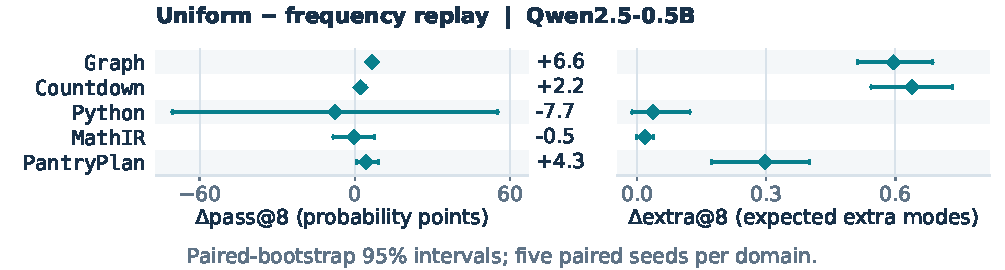
\includegraphics[width=\linewidth]{figures/replay_key_weighting.pdf}
\caption{\textbf{Uniform weighting preserves more verified alternatives.}
Uniform minus frequency-weighted replay at Qwen2.5-0.5B, Level 1, with five matched seeds. Extra modes are $B_8=\texttt{distinct@8}-\texttt{pass@8}$. Bars show nominal 95\% paired-seed bootstrap intervals. The mean gain is $.318$ extra modes, with an inconclusive correctness effect. Extra modes remain coupled to correctness; they do not measure success-conditional \pmd{}.}
\label{fig:replay-key-weighting}
\end{figure}

\clearpage
\section{Fixed Semantic-Entropy Factorials}
\label{app:semantic-current-factorial}
A fixed semantic-entropy bonus can be applied with or without verified replay.
Pantry semantic arms use the registered E85 repairs: original E81/E82/E83
Pantry runs received zero semantic advantage because of an outcome-key defect
and remain excluded. The historical Falcon factorial display had not applied
that repair; no value from its superseded Pantry column is reused here.
The matched four-arm studies compare its effect on Dr.GRPO, its effect on
Re:Dr.GRPO, and the difference of these effects. This restores the full
factorial detail beyond the main semantic-only comparator. We reconstruct
exact terminal four-draw endpoints under the current source-admission policy:
identical repeated metrics are deduplicated, unapproved conflicting retries
abort, and the previously excluded Falcon Countdown replay seed 59 remains
excluded. All three contrasts in that cell therefore use the common four
seeds 55--58; other 0.5B/1B cells use five. No old five-seed Falcon Countdown
interval is reused. Tables report paired seed means and pointwise Student-$t$
95\% intervals, without pooling models or domains.

The Qwen2.5-3B extension has only fixed seed 70 and no semantic-only arm.
Its on-replay comparison is descriptive, has no interval and cannot identify
a factorial interaction. These are fixed-coefficient experiments, not a
sweep over entropy strengths. Their endpoints do not establish that semantic
entropy reproduces the mechanism of a bank that revisits verified keys.
\begin{table}[H]
\centering
\caption{Qwen2.5-0.5B: fixed semantic-entropy effects. Without replay is semantic-only minus Dr.GRPO; on replay is semantic-plus-replay minus Re:Dr.GRPO; interaction subtracts the first effect from the second. Extra modes equal distinct@8 minus pass@8.}
\label{tab:semantic-current-qwen2505b}
\scriptsize
\setlength{\tabcolsep}{3pt}
\begin{tabular}{lr l rrr}
\toprule
Domain & $n$ & Contrast & $\Delta$ pass@8 & $\Delta$ distinct@8 & $\Delta$ extra modes \\
\midrule
Graph & 5 & Without replay & $0.002$ $[-0.028, 0.031]$ & $0.004$ $[-0.034, 0.041]$ & $0.002$ $[-0.010, 0.014]$ \\
Graph & 5 & On replay & $-0.002$ $[-0.027, 0.023]$ & $-0.022$ $[-0.179, 0.135]$ & $-0.020$ $[-0.161, 0.120]$ \\
Graph & 5 & Interaction & $-0.004$ $[-0.035, 0.028]$ & $-0.026$ $[-0.193, 0.141]$ & $-0.022$ $[-0.161, 0.116]$ \\
Countdown & 5 & Without replay & $0.141$ $[-0.047, 0.330]$ & $0.184$ $[0.011, 0.358]$ & $0.043$ $[0.001, 0.085]$ \\
Countdown & 5 & On replay & $-0.003$ $[-0.033, 0.028]$ & $0.115$ $[0.022, 0.209]$ & $0.118$ $[0.004, 0.232]$ \\
Countdown & 5 & Interaction & $-0.144$ $[-0.326, 0.037]$ & $-0.069$ $[-0.233, 0.095]$ & $0.075$ $[-0.051, 0.201]$ \\
Python & 5 & Without replay & $0.000$ $[0.000, 0.000]$ & $0.000$ $[0.000, 0.000]$ & $0.000$ $[0.000, 0.000]$ \\
Python & 5 & On replay & $-0.002$ $[-0.717, 0.714]$ & $0.016$ $[-0.747, 0.780]$ & $0.018$ $[-0.164, 0.200]$ \\
Python & 5 & Interaction & $-0.002$ $[-0.717, 0.714]$ & $0.016$ $[-0.747, 0.780]$ & $0.018$ $[-0.164, 0.200]$ \\
MathIR & 5 & Without replay & $-0.121$ $[-0.349, 0.106]$ & $-0.121$ $[-0.347, 0.105]$ & $0.001$ $[-0.006, 0.008]$ \\
MathIR & 5 & On replay & $0.031$ $[-0.035, 0.097]$ & $0.035$ $[-0.044, 0.114]$ & $0.004$ $[-0.047, 0.055]$ \\
MathIR & 5 & Interaction & $0.153$ $[-0.018, 0.324]$ & $0.156$ $[-0.050, 0.362]$ & $0.003$ $[-0.052, 0.058]$ \\
Pantry & 5 & Without replay & $0.201$ $[0.119, 0.283]$ & $1.120$ $[0.888, 1.352]$ & $0.919$ $[0.713, 1.124]$ \\
Pantry & 5 & On replay & $0.141$ $[0.044, 0.238]$ & $1.095$ $[0.368, 1.823]$ & $0.955$ $[0.321, 1.589]$ \\
Pantry & 5 & Interaction & $-0.061$ $[-0.161, 0.040]$ & $-0.025$ $[-0.826, 0.777]$ & $0.036$ $[-0.682, 0.754]$ \\
\bottomrule
\end{tabular}
\end{table}
\begin{table}[H]
\centering
\caption{Falcon3-1B: fixed semantic-entropy effects. Without replay is semantic-only minus Dr.GRPO; on replay is semantic-plus-replay minus Re:Dr.GRPO; interaction subtracts the first effect from the second. Extra modes equal distinct@8 minus pass@8.}
\label{tab:semantic-current-falcon31b}
\scriptsize
\setlength{\tabcolsep}{3pt}
\begin{tabular}{lr l rrr}
\toprule
Domain & $n$ & Contrast & $\Delta$ pass@8 & $\Delta$ distinct@8 & $\Delta$ extra modes \\
\midrule
Graph & 5 & Without replay & $0.036$ $[-0.192, 0.264]$ & $0.205$ $[-0.483, 0.893]$ & $0.169$ $[-0.292, 0.630]$ \\
Graph & 5 & On replay & $0.001$ $[-0.040, 0.043]$ & $-0.006$ $[-0.113, 0.101]$ & $-0.007$ $[-0.091, 0.077]$ \\
Graph & 5 & Interaction & $-0.035$ $[-0.237, 0.168]$ & $-0.211$ $[-0.886, 0.464]$ & $-0.176$ $[-0.649, 0.297]$ \\
Countdown & 4 & Without replay & $0.004$ $[-0.092, 0.100]$ & $-0.042$ $[-0.258, 0.173]$ & $-0.047$ $[-0.168, 0.074]$ \\
Countdown & 4 & On replay & $0.036$ $[-0.028, 0.101]$ & $0.047$ $[-0.082, 0.177]$ & $0.011$ $[-0.064, 0.087]$ \\
Countdown & 4 & Interaction & $0.032$ $[-0.098, 0.161]$ & $0.090$ $[-0.188, 0.367]$ & $0.058$ $[-0.099, 0.216]$ \\
Python & 5 & Without replay & $0.002$ $[-0.003, 0.008]$ & $0.002$ $[-0.003, 0.008]$ & $0.000$ $[0.000, 0.000]$ \\
Python & 5 & On replay & $-0.133$ $[-0.308, 0.043]$ & $-0.091$ $[-0.503, 0.321]$ & $0.042$ $[-0.296, 0.380]$ \\
Python & 5 & Interaction & $-0.135$ $[-0.310, 0.040]$ & $-0.093$ $[-0.507, 0.321]$ & $0.042$ $[-0.296, 0.380]$ \\
MathIR & 5 & Without replay & $-0.002$ $[-0.063, 0.060]$ & $-0.002$ $[-0.063, 0.060]$ & $0.000$ $[0.000, 0.000]$ \\
MathIR & 5 & On replay & $0.086$ $[0.004, 0.168]$ & $0.108$ $[0.003, 0.214]$ & $0.022$ $[-0.009, 0.054]$ \\
MathIR & 5 & Interaction & $0.087$ $[0.029, 0.146]$ & $0.110$ $[0.043, 0.176]$ & $0.022$ $[-0.009, 0.054]$ \\
Pantry & 5 & Without replay & $0.011$ $[-0.019, 0.041]$ & $0.091$ $[-0.161, 0.342]$ & $0.080$ $[-0.142, 0.301]$ \\
Pantry & 5 & On replay & $0.025$ $[-0.044, 0.094]$ & $0.382$ $[-0.702, 1.465]$ & $0.356$ $[-0.670, 1.382]$ \\
Pantry & 5 & Interaction & $0.014$ $[-0.052, 0.081]$ & $0.291$ $[-0.646, 1.228]$ & $0.277$ $[-0.615, 1.168]$ \\
\bottomrule
\end{tabular}
\end{table}
\begin{table}[H]
\centering
\caption{Qwen2.5-3B: fixed semantic-entropy effects. Without replay is semantic-only minus Dr.GRPO; on replay is semantic-plus-replay minus Re:Dr.GRPO; interaction subtracts the first effect from the second. Extra modes equal distinct@8 minus pass@8.}
\label{tab:semantic-current-qwen253b}
\scriptsize
\setlength{\tabcolsep}{3pt}
\begin{tabular}{lr l rrr}
\toprule
Domain & $n$ & Contrast & $\Delta$ pass@8 & $\Delta$ distinct@8 & $\Delta$ extra modes \\
\midrule
Graph & 1 & On replay & $-0.016$ & $-0.010$ & $0.006$ \\
Countdown & 1 & On replay & $0.039$ & $0.146$ & $0.107$ \\
Python & 1 & On replay & $-0.590$ & $-1.215$ & $-0.625$ \\
MathIR & 1 & On replay & $0.033$ & $0.010$ & $-0.023$ \\
Pantry & 1 & On replay & $0.035$ & $0.393$ & $0.357$ \\
\bottomrule
\end{tabular}
\end{table}
\path{results/semantic_current_summary_20260912.json} retains per-seed
endpoints, source hashes, exclusion evidence and all three metrics.
\path{ops/build_paper_semantic_current_summary.py} reconstructs these contrasts
with the same strict endpoint reader used by the current core comparison, including all documented exclusions.


\newpage
\section{Concentration and Replay Mechanisms}
\label{app:ablations}

\subsection{Concentration with 64 responses per prompt}
\label{app:fresh-concentration}

We evaluate initial and terminal checkpoints on the 128 held-out Level-1
\texttt{Graph} and \texttt{PantryPlan} prompts, drawing 64 responses per
prompt from new sampling streams. This evaluation is separate from the
32-response comparison in Fig.~\ref{fig:concentration-story}. It covers
Qwen2.5-0.5B, Falcon3-1B, and Qwen2.5-3B, with five training seeds for
Dr.GRPO, Re:Dr, MaxRL, and Re:Max. For each model, the five initial
evaluations use independent sampling from the same weights. Each initial
evaluation is paired with one training seed and shared across the four methods.

\paragraph{Matched comparisons.}
We estimate \pmd{} from correct-output pairs and average promptwise
differences over prompts with at least two correct responses in both
conditions, then average the five seed effects equally. Thus positive
changes indicate more diverse correct modes. Matching prompts within each
comparison differs from subtracting means over separately eligible prompts.
The eligible population ranges from 37 to 127 of the 128 prompts across
comparisons and seeds. Effects from different comparisons therefore cannot
be subtracted to reconstruct a trajectory on a common prompt population. Tables~\ref{tab:fresh-concentration-initial}
and~\ref{tab:fresh-concentration-replay} give all 36 contrasts and their
eligible-prompt ranges. Intervals are nominal 95\% paired Student-$t$
intervals with four degrees of freedom. They describe variation over the
five training-seed and initial-sampling pairs, conditional on the fixed
prompts and initial weights. They are unadjusted for multiple comparisons
and do not quantify uncertainty over unseen tasks.

\begin{figure}[t]
 \centering
 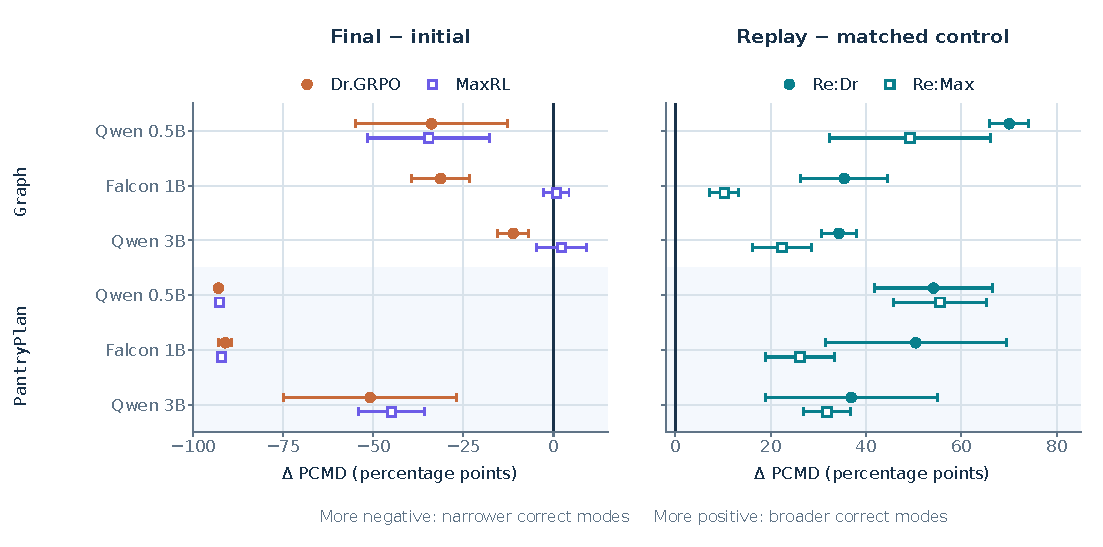
\includegraphics[width=\linewidth]{figures/fresh_concentration_pcmd_20260912.pdf}
 \caption{\textbf{Replay increases correct-mode diversity at a 64-response budget.}
 Left: Dr.GRPO reduces \pmd{} in all six model--domain comparisons;
 MaxRL's change is inconclusive for Falcon3-1B and Qwen2.5-3B \texttt{Graph}.
 Right: replay increases \pmd{} in all twelve comparisons with matched
 trained controls. Points show means over five paired seeds; bars give
 nominal 95\% Student-$t$ intervals. Each contrast uses its own jointly
 eligible Level-1 prompts. Horizontal scales differ between panels.}
 \label{fig:fresh-concentration}
\end{figure}

\paragraph{Concentration and mitigation.}
Dr.GRPO reduces \pmd{} in all six model--domain comparisons and all
30 seed effects. Replay increases \pmd{} relative to its matched trained
control under both objectives in all twelve comparisons and all 60 seed
effects. All eighteen nominal intervals exclude zero
(Fig.~\ref{fig:fresh-concentration}). These directions also hold when
pooling correct pairs, using each policy's own eligible prompts, or
restricting to the intersection of eligible prompts across seeds.
The intersection can be small: for Qwen2.5-0.5B \texttt{Graph}, only five
prompts are jointly eligible across all seeds in comparisons involving Dr.GRPO.

MaxRL alone does not consistently reduce diversity: its Falcon3-1B and
Qwen2.5-3B \texttt{Graph} intervals include zero. An improvement over a
trained control also need not restore initial diversity. Both replay
variants remain below initial \pmd{} in \texttt{PantryPlan} at every
scale, whereas their \texttt{Graph} comparisons exceed the initial value.
These results describe diversity within each comparison's eligible prompt
population; they do not establish recovery of the same individual modes.

\paragraph{Correctness, coverage, and sampling budget.}
All 24 trained-versus-initial comparisons increase per-response
correctness averaged over all evaluation prompts, in every seed. Nevertheless, every
\texttt{PantryPlan} method--scale comparison has lower \texttt{pass@64}
than initialization in every seed. Averaging over all evaluation prompts,
replay improves mean
\texttt{pass@8}, \texttt{distinct@8}, \texttt{pass@64}, and
\texttt{distinct@64} relative to its trained control in all twelve
comparisons; per-response correctness improves in seven of twelve.
On jointly eligible prompts, however, replay lowers mean correctness in
eleven of twelve comparisons. The concentration effects therefore do not
hold correctness fixed.

The eight-response metrics average over subsets of eight responses from
each 64-response pool (rarefaction). For Qwen2.5-3B \texttt{Graph}, Dr.GRPO increases per-response correctness by
14.49 percentage points and \texttt{distinct@8} by 0.112 modes per prompt,
while reducing \pmd{} by 11.20 points and \texttt{distinct@64} by
0.220 modes. The change in verified-mode count reverses sign between
eight and 64 responses in every seed. A gain at one sampling budget thus
need not persist at a larger budget. These evaluations measure the
distribution of correct responses and the modes observed in finite samples;
they do not establish exact mode extinction, recovery of the full support,
or a causal effect of diversity on accuracy.

% Generated by ops/build_paper_fresh_concentration.py; do not hand edit.
\begin{table}[t]
\centering
\small
\setlength{\tabcolsep}{4pt}
\caption{64-response evaluation: trained policy minus initialization. Changes in \pmd{} are in probability units; positive values indicate more diverse correct modes. Brackets give nominal 95\% paired Student-$t$ intervals ($n=5$, four degrees of freedom). The last column gives the range of jointly eligible prompts across seeds, out of 128. Each row uses its own matched prompt population.}
\label{tab:fresh-concentration-initial}
\begin{tabular}{llrr}
\toprule
Domain & Contrast & $\Delta\pmd$ [95\% interval] & Joint prompts \\
\midrule
\multicolumn{4}{l}{\textbf{Qwen2.5-0.5B}} \\
\texttt{Graph} & Dr.GRPO $-$ initial & $-0.338\;[-0.550, -0.126]$ & 37--45 \\
 & Re:Dr $-$ initial & $+0.217\;[+0.190, +0.243]$ & 97--103 \\
 & MaxRL $-$ initial & $-0.346\;[-0.516, -0.177]$ & 37--86 \\
 & Re:Max $-$ initial & $+0.155\;[+0.107, +0.203]$ & 97--101 \\
\texttt{PantryPlan} & Dr.GRPO $-$ initial & $-0.929\;[-0.936, -0.923]$ & 62--68 \\
 & Re:Dr $-$ initial & $-0.357\;[-0.445, -0.269]$ & 109--122 \\
 & MaxRL $-$ initial & $-0.927\;[-0.932, -0.921]$ & 62--71 \\
 & Re:Max $-$ initial & $-0.355\;[-0.438, -0.272]$ & 108--124 \\
\midrule
\multicolumn{4}{l}{\textbf{Falcon3-1B}} \\
\texttt{Graph} & Dr.GRPO $-$ initial & $-0.313\;[-0.393, -0.233]$ & 75--99 \\
 & Re:Dr $-$ initial & $+0.043\;[+0.006, +0.081]$ & 100--107 \\
 & MaxRL $-$ initial & $+0.008\;[-0.027, +0.043]$ & 104--109 \\
 & Re:Max $-$ initial & $+0.119\;[+0.096, +0.141]$ & 106--109 \\
\texttt{PantryPlan} & Dr.GRPO $-$ initial & $-0.910\;[-0.928, -0.893]$ & 81--86 \\
 & Re:Dr $-$ initial & $-0.378\;[-0.507, -0.250]$ & 104--110 \\
 & MaxRL $-$ initial & $-0.921\;[-0.925, -0.916]$ & 81 \\
 & Re:Max $-$ initial & $-0.519\;[-0.575, -0.462]$ & 106--116 \\
\midrule
\multicolumn{4}{l}{\textbf{Qwen2.5-3B}} \\
\texttt{Graph} & Dr.GRPO $-$ initial & $-0.112\;[-0.156, -0.069]$ & 78--86 \\
 & Re:Dr $-$ initial & $+0.226\;[+0.212, +0.240]$ & 88--96 \\
 & MaxRL $-$ initial & $+0.022\;[-0.048, +0.092]$ & 81--93 \\
 & Re:Max $-$ initial & $+0.254\;[+0.234, +0.274]$ & 90--96 \\
\texttt{PantryPlan} & Dr.GRPO $-$ initial & $-0.509\;[-0.750, -0.268]$ & 69--99 \\
 & Re:Dr $-$ initial & $-0.115\;[-0.157, -0.073]$ & 101--110 \\
 & MaxRL $-$ initial & $-0.449\;[-0.541, -0.358]$ & 83--98 \\
 & Re:Max $-$ initial & $-0.116\;[-0.208, -0.024]$ & 105--110 \\
\bottomrule
\end{tabular}
\end{table}

% Generated by ops/build_paper_fresh_concentration.py; do not hand edit.
\begin{table}[t]
\centering
\small
\setlength{\tabcolsep}{4pt}
\caption{64-response evaluation: replay minus its matched trained control. Changes in \pmd{} are in probability units; positive values indicate more diverse correct modes. Brackets give nominal 95\% paired Student-$t$ intervals ($n=5$, four degrees of freedom). The last column gives the range of jointly eligible prompts across seeds, out of 128. Each row uses its own matched prompt population.}
\label{tab:fresh-concentration-replay}
\begin{tabular}{llrr}
\toprule
Domain & Contrast & $\Delta\pmd$ [95\% interval] & Joint prompts \\
\midrule
\multicolumn{4}{l}{\textbf{Qwen2.5-0.5B}} \\
\texttt{Graph} & Re:Dr $-$ Dr.GRPO & $+0.700\;[+0.659, +0.742]$ & 40--46 \\
 & Re:Max $-$ MaxRL & $+0.493\;[+0.324, +0.662]$ & 41--107 \\
\texttt{PantryPlan} & Re:Dr $-$ Dr.GRPO & $+0.542\;[+0.418, +0.665]$ & 62--68 \\
 & Re:Max $-$ MaxRL & $+0.555\;[+0.458, +0.652]$ & 61--71 \\
\midrule
\multicolumn{4}{l}{\textbf{Falcon3-1B}} \\
\texttt{Graph} & Re:Dr $-$ Dr.GRPO & $+0.354\;[+0.264, +0.445]$ & 73--101 \\
 & Re:Max $-$ MaxRL & $+0.103\;[+0.072, +0.133]$ & 122--127 \\
\texttt{PantryPlan} & Re:Dr $-$ Dr.GRPO & $+0.505\;[+0.315, +0.694]$ & 80--84 \\
 & Re:Max $-$ MaxRL & $+0.262\;[+0.190, +0.334]$ & 81 \\
\midrule
\multicolumn{4}{l}{\textbf{Qwen2.5-3B}} \\
\texttt{Graph} & Re:Dr $-$ Dr.GRPO & $+0.343\;[+0.307, +0.380]$ & 94--107 \\
 & Re:Max $-$ MaxRL & $+0.224\;[+0.163, +0.286]$ & 105--123 \\
\texttt{PantryPlan} & Re:Dr $-$ Dr.GRPO & $+0.369\;[+0.188, +0.550]$ & 72--101 \\
 & Re:Max $-$ MaxRL & $+0.319\;[+0.270, +0.367]$ & 89--99 \\
\bottomrule
\end{tabular}
\end{table}

\FloatBarrier


\subsection{Conditional concentration from saved training outputs}
\label{app:conditional-concentration}

This retrospective analysis distinguishes the distribution of correct keys
from the probability of producing a correct output. If $P=0$, $C$ is undefined
and $B_2=0$. For a fixed prompt with
correct mass $P>0$, write $q_c=\Pr[V(Y,s_x)=c\mid V(Y,s_x)\ne\bot]$ and define
\begin{equation}
 C(q)=\sum_c q_c^2,\qquad B_2=2P-P^2C(q).
 \label{eq:collision-breadth-bridge}
\end{equation}
The first quantity is the probability that two independent correct outputs
share a key. The second identity follows by expanding
$B_2=\sum_c[1-(1-Pq_c)^2]$. It makes explicit why sampled breadth can
change through correctness or conditional concentration. A decrease in $C$
alone does not imply majorization, larger total support, or recovery of any
particular mode. In particular, observed collisions cannot establish that
an unobserved key has exactly zero probability under the policy.

\paragraph{Connection to the conditional theory.}
Under the assumptions of Theorem~\ref{thm:grpo-collapse}, the time change in
its proof gives $dq_c/d\tau=q_c(q_c-C)$. Consequently,
\begin{equation}
 \frac{dC}{d\tau}
 =2\left(\sum_c q_c^3-C^2\right)
 =2\operatorname{Var}_{c\sim q}(q_c)\ge0.
 \label{eq:collision-flow}
\end{equation}
The variance vanishes exactly when $q$ is uniform on its positive support.
Thus concentration is monotone along this ideal categorical flow, with
strict increase whenever the positive coordinates are unequal. The identity
provides a theoretical basis for the diagnostic; it does not establish
monotonicity for the implemented neural optimizer or a corresponding
monotonic decrease under finite-bank replay.

\paragraph{Estimator and identifiable population.}
The pair statistic is the one defined in App.~\ref{app:metric-sampling}, read
here in the collision orientation, $\widehat C=1-\widehat{\pmd}$, over a prompt's
$R\ge2$ correct samples: the contrast this analysis reports is about
concentration, so the orientation that rises with it is the one to print. Its
promptwise unbiasedness, and the limits of that identity under joint selection,
are established there. We leave $R<2$ undefined, rather than assigning a
concentration value to insufficient correct observations.

For each paired training seed $s$, let $E_s$ contain exactly the prompts with
a defined estimate in both conditions. The reported seed contrast is
$|E_s|^{-1}\sum_{x\in E_s}(\widehat C_{B,x}-\widehat C_{A,x})$ when
$E_s$ is nonempty. We then weight defined training seeds equally, preserving
all registered blocks and their missingness. Before/after contrasts use each
method's own initial checkpoint and step 3,072; replay contrasts compare
matched terminal conditions. No other method substitutes for a missing
initial evaluation. Five defined seeds receive nominal Student-$t$ intervals;
partial blocks are descriptive. These intervals describe the measured seed
means and are not simultaneous guarantees or uncertainty over unseen prompts.

The hosted analysis uses the same promptwise collision concept but pools
correct pairs. At a common sampling budget, the ratio of expected colliding
and correct pair counts is
$\sum_x P_x^2 C(q_x)/\sum_x P_x^2$. Its finite-sample ratio is not generally
unbiased for that target. The training contrast here weights eligible prompts
equally. Changing correctness can change either eligibility or hosted pair
weights, so the two aggregate values are not directly interchangeable.

\paragraph{Retrospective protocol and source coverage.}
The estimator and comparisons were recorded before the initial concentration
contrasts, with the sampling-stream amendment also preceding those effects.
Two retrospective extensions then followed the paper's completed source
census. The first included thirteen newly available terminal checkpoints
and withdrew one conflicted initial checkpoint. The September~12 extension
adds all ten remaining Level-2 Pantry terminal checkpoints, reusing 752
unchanged checkpoint identities and changing no estimator or eligibility
rule. All prior results, caches, and source snapshots remain preserved.
The final collection contains 475 registered runs and 902 available
checkpoint evaluations, with 74 Dr.GRPO and 75 MaxRL Level-1 replay pairs
and 25 pairs per objective at Level~2 before conditional eligibility.
Complete terminal coverage neither supplies missing initial outputs nor
makes every conditional contrast identifiable. Exact source hashes and
both retrospective extensions' timing remain bound to the result artifact.

\paragraph{Sampling-stream audit.}
Four saved eight-output groups do not provide 32 independently seeded
responses. The recorded parent seeds increment by one; the audited vLLM V0
sampler increments each child's seed by its output index. The resulting
nominal stream ranges overlap, giving eleven distinct identifiers. For each
prompt and checkpoint we retain the earliest draw/output position for every
identifier, independently of correctness or key identity. Repeated positions
sometimes disagree, so identical seed integers are not treated as a proof of
identical outputs. Archived actor source is available for 150 of the 400
factorial cells and none of the 75 additional GRPO cells; historical dependency
identity is not cryptographically established for every run. The stream
mapping rests on the audited implementation and recorded neutral request
contract, with the historical-runtime assumption stated explicitly.

The primary eleven-stream comparisons reuse nominal streams across conditions
and remain descriptive after common eligibility. Two additional orientations
compare the lower five identifiers in condition A with the upper six in B,
then reverse the assignment. Each orientation retains its own eligible prompts
and seed counts. Shared identifiers also recur across prompts; neither their
separation across conditions nor these selected-population means establishes
independent prompt observations. Independent fixed-law sampling is an explicit
assumption of the estimator identity, not a conclusion of the source audit.

Original \texttt{mean@8}, \texttt{pass@8}, and \texttt{distinct@8} remain averages
over the four intact groups, reconstructed from all saved verified keys.
Cross-group overlap affects dependence, not linearity of those marginal
averages. The complete result artifact also retains each intact-group
collision comparison, a fixed-first-group check, fixed-across-seed prompt
intersections, and four-condition change differences. A naive concatenated
32-position collision is retained solely as a reuse diagnostic. These views
are not treated as independent replications or substituted for missing cells.

\paragraph{Findings and their limits.}
In Graph and PantryPlan, all twelve Dr.GRPO/GRPO before/after comparisons
across the three scales show increased conditional concentration, with
nominal intervals above zero. Correctness also increases on those same
eligible prompts. Graph's increases range from $.098$ to $.274$; PantryPlan's
range from $.447$ to $.887$. The two disjoint orientations agree in direction
in eleven of these twelve blocks; Falcon Graph with GRPO is the exception.
The evidence therefore supports observed training-induced concentration in
these tasks, with a visible sampling sensitivity, rather than a universal
claim about every RLVR run or exact disappearance of modes.

Re:Dr lowers concentration relative to Dr.GRPO in all six Graph and
PantryPlan comparisons: changes range from $-.756$ to $-.273$ in Graph and
$-.433$ to $-.300$ in PantryPlan. Both disjoint orientations agree in direction
in all six, and their primary nominal intervals lie below zero. These
comparisons also have lower per-sample correctness on their jointly eligible
prompts. They establish a change in the conditional correct-key distribution
on that observable population; they do not hold correctness fixed or imply
that every accuracy measure improves on the same prompts. Full-test
\texttt{pass@8} and sampled breadth remain the separately reported primary
outcomes of the replay experiment.

The other domains constrain the interpretation. Dr.GRPO/GRPO Python initial
outputs provide no jointly eligible prompts at this budget, so their
longitudinal collision contrast is unidentified. Some Countdown initial
comparisons use only one or two eligible prompts per seed. Several MathIR
conditions already have observed collision one, leaving little detectable
change. MaxRL comparisons, incomplete saved-output cohorts, and the two
sampling orientations are reported explicitly in the following tables;
we do not infer a universal concentration benefit from raw breadth gains.

In the completed 3B MaxRL replay cohort, Countdown, Python, and PantryPlan
show lower concentration with nominal intervals below zero; MathIR's measured
contrast is zero. Graph's primary contrast is negative, but its two disjoint
orientations disagree in direction, as they do for Falcon Graph with MaxRL.
At Level 2, both Graph replay contrasts are negative with agreement across
orientations. Complete PantryPlan training still leaves sparse conditional
populations: Re:Dr has a defined collision contrast for three seeds
(2--16 eligible prompts), with mean $+.495$; Re:Max has four defined
seeds (1--19 eligible prompts), with mean $+.439$. Their disjoint-orientation
means are also positive but retain fewer defined seeds. Neither contrast
receives a five-seed interval. Thus the full endpoint breadth gains coexist
with increased concentration on these small jointly correct subsets; they
do not establish uniformly reduced conditional concentration.

% Generated by ops/exp_scaling/build_paper_conditional_concentration_appendix.py.
\begin{table}[!htbp]
\centering
\scriptsize
\setlength{\tabcolsep}{3pt}
\begin{tabular}{@{}llcrlrrr@{}}
\toprule
Domain & Objective & $n$ & $\Delta\widehat C$ & nominal 95\% interval & $|E_s|$ & split 0 ($n$) & split 1 ($n$) \\
\midrule
\texttt{Graph} & Dr.GRPO & 5 & +0.242 & [+0.110, +0.373] & 17--40 & +0.257 (5) & +0.284 (5) \\
\texttt{Graph} & GRPO & 5 & +0.221 & [+0.097, +0.344] & 15--28 & +0.268 (5) & +0.287 (5) \\
\texttt{Graph} & MaxRL & 5 & +0.145 & [-0.033, +0.324] & 18--40 & +0.115 (5) & +0.174 (5) \\
\texttt{Graph} & Re:Dr & 5 & -0.507 & [-0.558, -0.456] & 45--49 & -0.519 (5) & -0.465 (5) \\
\texttt{Graph} & Re:Max & 5 & -0.399 & [-0.458, -0.339] & 40--51 & -0.436 (5) & -0.348 (5) \\
\texttt{Countdown} & Dr.GRPO & 5 & +1.000 & [+1.000, +1.000] & 1--2 & -- (0) & +1.000 (5) \\
\texttt{Countdown} & GRPO & 5 & +0.964 & [+0.863, +1.065] & 1--2 & -- (0) & +0.920 (5) \\
\texttt{Countdown} & MaxRL & 4 & +0.977 & -- & 0--2 & -- (0) & +1.000 (4) \\
\texttt{Countdown} & Re:Dr & 5 & +0.467 & [+0.117, +0.816] & 1--3 & -- (0) & +0.713 (4) \\
\texttt{Countdown} & Re:Max & 5 & +0.420 & [+0.359, +0.480] & 1--2 & -- (0) & +0.493 (5) \\
\texttt{Python} & Dr.GRPO & 0 & -- & -- & 0 & -- (0) & -- (0) \\
\texttt{Python} & GRPO & 0 & -- & -- & 0 & -- (0) & -- (0) \\
\texttt{Python} & MaxRL & 0 & -- & -- & 0 & -- (0) & -- (0) \\
\texttt{Python} & Re:Dr & 0 & -- & -- & 0 & -- (0) & -- (0) \\
\texttt{Python} & Re:Max & 0 & -- & -- & 0 & -- (0) & -- (0) \\
\texttt{MathIR} & Dr.GRPO & 5 & +0.000 & [+0.000, +0.000] & 5--8 & +0.000 (5) & +0.000 (1) \\
\texttt{MathIR} & GRPO & 5 & +0.040 & [-0.071, +0.151] & 4--10 & +0.000 (5) & +0.250 (2) \\
\texttt{MathIR} & MaxRL & 5 & +0.022 & [-0.039, +0.084] & 5--9 & +0.000 (5) & +0.067 (5) \\
\texttt{MathIR} & Re:Dr & 5 & +0.059 & [-0.046, +0.163] & 8--11 & +0.000 (5) & +0.367 (2) \\
\texttt{MathIR} & Re:Max & 5 & +0.063 & [-0.009, +0.134] & 9--11 & +0.000 (5) & +0.250 (5) \\
\texttt{PantryPlan} & Dr.GRPO & 5 & +0.833 & [+0.819, +0.847] & 54--64 & +1.000 (5) & +1.000 (5) \\
\texttt{PantryPlan} & GRPO & 5 & +0.849 & [+0.845, +0.853] & 64--65 & +1.000 (5) & +1.000 (5) \\
\texttt{PantryPlan} & MaxRL & 5 & +0.859 & [+0.836, +0.881] & 54--65 & +1.000 (5) & +1.000 (5) \\
\texttt{PantryPlan} & Re:Dr & 5 & +0.413 & [+0.345, +0.481] & 78--89 & +0.543 (5) & +0.538 (5) \\
\texttt{PantryPlan} & Re:Max & 5 & +0.446 & [+0.324, +0.567] & 80--88 & +0.593 (5) & +0.550 (5) \\
\bottomrule
\end{tabular}
\caption{\textbf{Initial-to-final conditional concentration: Qwen2.5-0.5B, Level 1.} Each row compares the same method at initialization and step 3,072; positive $\Delta\widehat C$ means greater concentration among correct outputs. $n$ counts seeds with defined estimates; $|E_s|$ gives the range of eligible prompt counts. Splits 0 and 1 reverse the assignment of disjoint stream identifiers, with eligibility determined separately. Nominal 95\% Student-$t$ intervals require five defined seed estimates.}
\end{table}

\begin{table}[!htbp]
\centering
\scriptsize
\setlength{\tabcolsep}{3pt}
\begin{tabular}{@{}llcrlrrr@{}}
\toprule
Domain & Objective & $n$ & $\Delta\widehat C$ & nominal 95\% interval & $|E_s|$ & split 0 ($n$) & split 1 ($n$) \\
\midrule
\texttt{Graph} & Dr.GRPO & 5 & +0.233 & [+0.124, +0.343] & 41--54 & +0.059 (5) & +0.428 (5) \\
\texttt{Graph} & GRPO & 5 & +0.098 & [+0.026, +0.170] & 48--56 & -0.186 (5) & +0.273 (5) \\
\texttt{Graph} & MaxRL & 3 & -0.113 & -- & 48--52 & -0.083 (3) & +0.039 (3) \\
\texttt{Graph} & Re:Dr & 5 & -0.007 & [-0.065, +0.050] & 37--45 & +0.048 (5) & +0.045 (5) \\
\texttt{Graph} & Re:Max & 2 & -0.062 & -- & 51--52 & -0.300 (2) & -0.015 (2) \\
\texttt{Countdown} & Dr.GRPO & 5 & +0.022 & [-0.038, +0.082] & 6--8 & +0.000 (5) & -- (0) \\
\texttt{Countdown} & GRPO & 5 & +0.180 & [+0.128, +0.231] & 6--11 & +0.126 (5) & -- (0) \\
\texttt{Countdown} & MaxRL & 2 & +0.182 & -- & 11 & +0.143 (2) & -- (0) \\
\texttt{Countdown} & Re:Dr & 4 & +0.035 & -- & 10--11 & +0.158 (4) & -- (0) \\
\texttt{Countdown} & Re:Max & 1 & +0.135 & -- & 11 & +0.143 (1) & -- (0) \\
\texttt{Python} & Dr.GRPO & 0 & -- & -- & 0 & -- (0) & -- (0) \\
\texttt{Python} & GRPO & 0 & -- & -- & 0 & -- (0) & -- (0) \\
\texttt{Python} & MaxRL & 0 & -- & -- & 0 & -- (0) & -- (0) \\
\texttt{Python} & Re:Dr & 0 & -- & -- & 0 & -- (0) & -- (0) \\
\texttt{Python} & Re:Max & 0 & -- & -- & -- & -- (0) & -- (0) \\
\texttt{MathIR} & Dr.GRPO & 5 & +0.105 & [+0.088, +0.122] & 6 & -- (0) & +0.098 (5) \\
\texttt{MathIR} & GRPO & 5 & +0.054 & [-0.099, +0.206] & 3--7 & -- (0) & +0.233 (5) \\
\texttt{MathIR} & MaxRL & 1 & +0.278 & -- & 6 & +1.000 (1) & +0.133 (1) \\
\texttt{MathIR} & Re:Dr & 5 & +0.086 & [+0.026, +0.146] & 6--7 & -- (0) & +0.111 (5) \\
\texttt{MathIR} & Re:Max & 2 & +0.167 & -- & 5--6 & +1.000 (2) & +0.000 (2) \\
\texttt{PantryPlan} & Dr.GRPO & 5 & +0.886 & [+0.886, +0.886] & 76 & +1.000 (5) & +1.000 (5) \\
\texttt{PantryPlan} & GRPO & 5 & +0.863 & [+0.798, +0.928] & 76 & +0.945 (5) & +1.000 (5) \\
\texttt{PantryPlan} & MaxRL & 1 & +0.886 & -- & 76 & +1.000 (1) & +1.000 (1) \\
\texttt{PantryPlan} & Re:Dr & 4 & +0.437 & -- & 75--83 & +0.451 (4) & +0.618 (4) \\
\texttt{PantryPlan} & Re:Max & 2 & +0.746 & -- & 76--78 & +0.740 (2) & +0.978 (2) \\
\bottomrule
\end{tabular}
\caption{\textbf{Initial-to-final conditional concentration: Falcon3-1B, Level 1.} Each row compares the same method at initialization and step 3,072; positive $\Delta\widehat C$ means greater concentration among correct outputs. $n$ counts seeds with defined estimates; $|E_s|$ gives the range of eligible prompt counts. Splits 0 and 1 reverse the assignment of disjoint stream identifiers, with eligibility determined separately. Nominal 95\% Student-$t$ intervals require five defined seed estimates.}
\end{table}

\begin{table}[!htbp]
\centering
\scriptsize
\setlength{\tabcolsep}{3pt}
\begin{tabular}{@{}llcrlrrr@{}}
\toprule
Domain & Objective & $n$ & $\Delta\widehat C$ & nominal 95\% interval & $|E_s|$ & split 0 ($n$) & split 1 ($n$) \\
\midrule
\texttt{Graph} & Dr.GRPO & 5 & +0.274 & [+0.232, +0.316] & 44--47 & +0.030 (5) & +0.339 (5) \\
\texttt{Graph} & GRPO & 5 & +0.274 & [+0.207, +0.341] & 46--49 & +0.046 (5) & +0.364 (5) \\
\texttt{Graph} & MaxRL & 5 & +0.072 & [-0.002, +0.145] & 45--55 & -0.208 (5) & +0.215 (5) \\
\texttt{Graph} & Re:Dr & 5 & -0.038 & [-0.060, -0.016] & 48--53 & -0.227 (5) & +0.121 (5) \\
\texttt{Graph} & Re:Max & 5 & -0.145 & [-0.198, -0.093] & 46--52 & -0.220 (5) & +0.165 (5) \\
\texttt{Countdown} & Dr.GRPO & 5 & +0.160 & [+0.109, +0.211] & 11--12 & +0.200 (5) & -0.016 (5) \\
\texttt{Countdown} & GRPO & 5 & +0.182 & [+0.182, +0.182] & 11 & +0.200 (5) & +0.000 (5) \\
\texttt{Countdown} & MaxRL & 5 & +0.056 & [-0.046, +0.159] & 9--11 & +0.050 (5) & +0.000 (5) \\
\texttt{Countdown} & Re:Dr & 5 & +0.020 & [-0.060, +0.099] & 11--15 & +0.169 (5) & -0.071 (5) \\
\texttt{Countdown} & Re:Max & 5 & -0.100 & [-0.145, -0.055] & 10--12 & +0.000 (5) & -0.050 (5) \\
\texttt{Python} & Dr.GRPO & 0 & -- & -- & 0 & -- (0) & -- (0) \\
\texttt{Python} & GRPO & 0 & -- & -- & 0 & -- (0) & -- (0) \\
\texttt{Python} & MaxRL & 5 & +0.000 & [+0.000, +0.000] & 2--9 & +0.000 (2) & +0.000 (5) \\
\texttt{Python} & Re:Dr & 0 & -- & -- & 0 & -- (0) & -- (0) \\
\texttt{Python} & Re:Max & 5 & -0.023 & [-0.050, +0.003] & 9 & +0.000 (5) & -0.040 (5) \\
\texttt{MathIR} & Dr.GRPO & 5 & +0.000 & [+0.000, +0.000] & 11--14 & +0.000 (5) & +0.000 (5) \\
\texttt{MathIR} & GRPO & 5 & +0.000 & [+0.000, +0.000] & 9--11 & +0.000 (5) & +0.000 (5) \\
\texttt{MathIR} & MaxRL & 5 & +0.000 & [+0.000, +0.000] & 7--14 & +0.000 (5) & +0.000 (5) \\
\texttt{MathIR} & Re:Dr & 4 & -0.012 & -- & 14 & +0.000 (4) & +0.000 (4) \\
\texttt{MathIR} & Re:Max & 5 & +0.000 & [+0.000, +0.000] & 12--15 & +0.000 (5) & +0.000 (5) \\
\texttt{PantryPlan} & Dr.GRPO & 5 & +0.447 & [+0.266, +0.627] & 49--67 & +0.478 (5) & +0.245 (5) \\
\texttt{PantryPlan} & GRPO & 5 & +0.469 & [+0.411, +0.526] & 49--62 & +0.514 (5) & +0.271 (5) \\
\texttt{PantryPlan} & MaxRL & 5 & +0.431 & [+0.297, +0.565] & 59--69 & +0.394 (5) & +0.246 (5) \\
\texttt{PantryPlan} & Re:Dr & 5 & +0.184 & [+0.081, +0.288] & 64--71 & +0.087 (5) & +0.037 (5) \\
\texttt{PantryPlan} & Re:Max & 5 & +0.142 & [+0.018, +0.266] & 68--75 & +0.046 (5) & -0.015 (5) \\
\bottomrule
\end{tabular}
\caption{\textbf{Initial-to-final conditional concentration: Qwen2.5-3B, Level 1.} Each row compares the same method at initialization and step 3,072; positive $\Delta\widehat C$ means greater concentration among correct outputs. $n$ counts seeds with defined estimates; $|E_s|$ gives the range of eligible prompt counts. Splits 0 and 1 reverse the assignment of disjoint stream identifiers, with eligibility determined separately. Nominal 95\% Student-$t$ intervals require five defined seed estimates.}
\end{table}

\begin{table}[!htbp]
\centering
\scriptsize
\setlength{\tabcolsep}{3pt}
\begin{tabular}{@{}llcrlrrr@{}}
\toprule
Domain & Objective & $n$ & $\Delta\widehat C$ & nominal 95\% interval & $|E_s|$ & split 0 ($n$) & split 1 ($n$) \\
\midrule
\texttt{Graph} & Dr.GRPO & 5 & +0.625 & [+0.295, +0.955] & 2--10 & +0.633 (2) & +0.860 (5) \\
\texttt{Graph} & MaxRL & 5 & +0.452 & [+0.387, +0.518] & 6--10 & +0.767 (4) & +0.484 (5) \\
\texttt{Graph} & Re:Dr & 5 & -0.204 & [-0.282, -0.126] & 9--11 & +0.033 (5) & -0.372 (5) \\
\texttt{Graph} & Re:Max & 5 & -0.128 & [-0.262, +0.006] & 9--11 & +0.333 (5) & -0.267 (5) \\
\texttt{Countdown} & Dr.GRPO & 1 & +0.000 & -- & 0--1 & -- (0) & -- (0) \\
\texttt{Countdown} & MaxRL & 1 & +0.000 & -- & 0--1 & -- (0) & -- (0) \\
\texttt{Countdown} & Re:Dr & 5 & +0.000 & [+0.000, +0.000] & 1 & -- (0) & -- (0) \\
\texttt{Countdown} & Re:Max & 3 & +0.000 & -- & 0--1 & -- (0) & -- (0) \\
\texttt{Python} & Dr.GRPO & 5 & +0.302 & [+0.302, +0.302] & 32 & +0.000 (5) & +0.378 (5) \\
\texttt{Python} & MaxRL & 5 & +0.302 & [+0.302, +0.302] & 32 & +0.000 (5) & +0.378 (5) \\
\texttt{Python} & Re:Dr & 5 & +0.094 & [-0.259, +0.448] & 32 & -0.224 (5) & +0.146 (5) \\
\texttt{Python} & Re:Max & 5 & +0.199 & [-0.088, +0.485] & 32 & -0.070 (5) & +0.258 (5) \\
\texttt{MathIR} & Dr.GRPO & 3 & +0.000 & -- & 0--5 & -- (0) & +0.000 (3) \\
\texttt{MathIR} & MaxRL & 4 & +0.000 & -- & 0--6 & -- (0) & +0.000 (4) \\
\texttt{MathIR} & Re:Dr & 5 & +0.000 & [+0.000, +0.000] & 6 & -- (0) & +0.000 (5) \\
\texttt{MathIR} & Re:Max & 4 & +0.000 & -- & 6 & -- (0) & +0.000 (4) \\
\texttt{PantryPlan} & Dr.GRPO & 3 & -0.578 & -- & 0--3 & -0.500 (1) & -1.000 (1) \\
\texttt{PantryPlan} & MaxRL & 3 & -0.238 & -- & 1--5 & -1.000 (1) & -1.000 (1) \\
\texttt{PantryPlan} & Re:Dr & 2 & -0.049 & -- & 15--16 & -0.075 (2) & -0.050 (2) \\
\texttt{PantryPlan} & Re:Max & 3 & +0.020 & -- & 18--20 & +0.092 (3) & -0.174 (3) \\
\bottomrule
\end{tabular}
\caption{\textbf{Initial-to-final conditional concentration: Qwen2.5-0.5B, Level 2.} Each row compares the same method at initialization and step 3,072; positive $\Delta\widehat C$ means greater concentration among correct outputs. $n$ counts seeds with defined estimates; $|E_s|$ gives the range of eligible prompt counts. Splits 0 and 1 reverse the assignment of disjoint stream identifiers, with eligibility determined separately. Nominal 95\% Student-$t$ intervals require five defined seed estimates.}
\end{table}

\begin{table}[!htbp]
\centering
\scriptsize
\setlength{\tabcolsep}{3pt}
\begin{tabular}{@{}llcrlrrr@{}}
\toprule
Domain & Control & $n$ & $\Delta\widehat C$ & nominal 95\% interval & $|E_s|$ & split 0 ($n$) & split 1 ($n$) \\
\midrule
\texttt{Graph} & Dr.GRPO & 5 & -0.756 & [-0.831, -0.680] & 37--40 & -0.853 (5) & -0.807 (5) \\
\texttt{Graph} & MaxRL & 5 & -0.587 & [-0.759, -0.414] & 41--73 & -0.625 (5) & -0.605 (5) \\
\texttt{Countdown} & Dr.GRPO & 5 & -0.529 & [-0.605, -0.452] & 42--78 & -0.529 (5) & -0.535 (5) \\
\texttt{Countdown} & MaxRL & 5 & -0.547 & [-0.635, -0.459] & 45--84 & -0.578 (5) & -0.530 (5) \\
\texttt{Python} & Dr.GRPO & 5 & -0.090 & [-0.341, +0.160] & 22 & -0.115 (5) & -0.062 (5) \\
\texttt{Python} & MaxRL & 5 & -0.266 & [-0.577, +0.044] & 22 & -0.298 (5) & -0.272 (5) \\
\texttt{MathIR} & Dr.GRPO & 5 & -0.008 & [-0.017, +0.001] & 44--68 & -0.006 (5) & -0.008 (5) \\
\texttt{MathIR} & MaxRL & 5 & -0.005 & [-0.013, +0.003] & 32--56 & -0.007 (5) & -0.002 (5) \\
\texttt{PantryPlan} & Dr.GRPO & 5 & -0.433 & [-0.518, -0.347] & 54--66 & -0.442 (5) & -0.494 (5) \\
\texttt{PantryPlan} & MaxRL & 5 & -0.417 & [-0.547, -0.288] & 53--71 & -0.363 (5) & -0.508 (5) \\
\bottomrule
\end{tabular}
\caption{\textbf{Replay and conditional concentration: Qwen2.5-0.5B, Level 1.} Each row gives Re:Dr minus Dr.GRPO or Re:Max minus MaxRL at step 3,072; negative $\Delta\widehat C$ means lower concentration among correct outputs. $n$ counts seeds with defined estimates; $|E_s|$ gives the range of eligible prompt counts. Splits 0 and 1 reverse the assignment of disjoint stream identifiers, with eligibility determined separately. Nominal 95\% Student-$t$ intervals require five defined seed estimates.}
\end{table}

\begin{table}[!htbp]
\centering
\scriptsize
\setlength{\tabcolsep}{3pt}
\begin{tabular}{@{}llcrlrrr@{}}
\toprule
Domain & Control & $n$ & $\Delta\widehat C$ & nominal 95\% interval & $|E_s|$ & split 0 ($n$) & split 1 ($n$) \\
\midrule
\texttt{Graph} & Dr.GRPO & 5 & -0.309 & [-0.523, -0.094] & 31--64 & -0.129 (5) & -0.452 (5) \\
\texttt{Graph} & MaxRL & 5 & -0.021 & [-0.040, -0.002] & 95--100 & +0.100 (5) & -0.013 (5) \\
\texttt{Countdown} & Dr.GRPO & 4 & -0.168 & -- & 33--42 & -0.139 (4) & -0.233 (4) \\
\texttt{Countdown} & MaxRL & 5 & -0.063 & [-0.079, -0.047] & 78--81 & -0.062 (5) & -0.063 (5) \\
\texttt{Python} & Dr.GRPO & 0 & -- & -- & 0 & -- (0) & -- (0) \\
\texttt{Python} & MaxRL & 5 & -0.093 & [-0.350, +0.165] & 22--128 & -0.039 (5) & -0.090 (5) \\
\texttt{MathIR} & Dr.GRPO & 5 & +0.004 & [-0.007, +0.015] & 9--14 & +0.000 (5) & +0.000 (5) \\
\texttt{MathIR} & MaxRL & 5 & -0.001 & [-0.010, +0.009] & 40--72 & +0.000 (5) & +0.000 (5) \\
\texttt{PantryPlan} & Dr.GRPO & 5 & -0.404 & [-0.600, -0.209] & 74--81 & -0.435 (5) & -0.352 (5) \\
\texttt{PantryPlan} & MaxRL & 5 & -0.129 & [-0.223, -0.035] & 81 & -0.203 (5) & -0.043 (5) \\
\bottomrule
\end{tabular}
\caption{\textbf{Replay and conditional concentration: Falcon3-1B, Level 1.} Each row gives Re:Dr minus Dr.GRPO or Re:Max minus MaxRL at step 3,072; negative $\Delta\widehat C$ means lower concentration among correct outputs. $n$ counts seeds with defined estimates; $|E_s|$ gives the range of eligible prompt counts. Splits 0 and 1 reverse the assignment of disjoint stream identifiers, with eligibility determined separately. Nominal 95\% Student-$t$ intervals require five defined seed estimates.}
\end{table}

\begin{table}[!htbp]
\centering
\scriptsize
\setlength{\tabcolsep}{3pt}
\begin{tabular}{@{}llcrlrrr@{}}
\toprule
Domain & Control & $n$ & $\Delta\widehat C$ & nominal 95\% interval & $|E_s|$ & split 0 ($n$) & split 1 ($n$) \\
\midrule
\texttt{Graph} & Dr.GRPO & 5 & -0.273 & [-0.299, -0.247] & 54--71 & -0.363 (5) & -0.151 (5) \\
\texttt{Graph} & MaxRL & 5 & -0.162 & [-0.261, -0.062] & 68--83 & -0.169 (5) & +0.059 (5) \\
\texttt{Countdown} & Dr.GRPO & 5 & -0.137 & [-0.183, -0.090] & 70--75 & -0.153 (5) & -0.139 (5) \\
\texttt{Countdown} & MaxRL & 5 & -0.105 & [-0.126, -0.084] & 56--76 & -0.113 (5) & -0.095 (5) \\
\texttt{Python} & Dr.GRPO & 2 & -0.190 & -- & 0--22 & -0.221 (2) & -0.141 (2) \\
\texttt{Python} & MaxRL & 5 & -0.153 & [-0.265, -0.041] & 22--81 & -0.203 (5) & -0.083 (5) \\
\texttt{MathIR} & Dr.GRPO & 5 & -0.010 & [-0.022, +0.003] & 23--34 & -0.017 (5) & +0.003 (5) \\
\texttt{MathIR} & MaxRL & 5 & +0.000 & [+0.000, +0.000] & 21--27 & +0.000 (5) & +0.000 (5) \\
\texttt{PantryPlan} & Dr.GRPO & 5 & -0.300 & [-0.420, -0.179] & 71--83 & -0.337 (5) & -0.305 (5) \\
\texttt{PantryPlan} & MaxRL & 5 & -0.292 & [-0.319, -0.265] & 81--89 & -0.355 (5) & -0.237 (5) \\
\bottomrule
\end{tabular}
\caption{\textbf{Replay and conditional concentration: Qwen2.5-3B, Level 1.} Each row gives Re:Dr minus Dr.GRPO or Re:Max minus MaxRL at step 3,072; negative $\Delta\widehat C$ means lower concentration among correct outputs. $n$ counts seeds with defined estimates; $|E_s|$ gives the range of eligible prompt counts. Splits 0 and 1 reverse the assignment of disjoint stream identifiers, with eligibility determined separately. Nominal 95\% Student-$t$ intervals require five defined seed estimates.}
\end{table}

\begin{table}[!htbp]
\centering
\scriptsize
\setlength{\tabcolsep}{3pt}
\begin{tabular}{@{}llcrlrrr@{}}
\toprule
Domain & Control & $n$ & $\Delta\widehat C$ & nominal 95\% interval & $|E_s|$ & split 0 ($n$) & split 1 ($n$) \\
\midrule
\texttt{Graph} & Dr.GRPO & 5 & -0.577 & [-0.736, -0.418] & 9--25 & -0.599 (5) & -0.544 (5) \\
\texttt{Graph} & MaxRL & 5 & -0.405 & [-0.472, -0.339] & 28--42 & -0.262 (5) & -0.416 (5) \\
\texttt{Countdown} & Dr.GRPO & 4 & -0.230 & -- & 0--9 & -0.281 (4) & -0.292 (4) \\
\texttt{Countdown} & MaxRL & 4 & -0.073 & -- & 0--10 & +0.000 (3) & -0.118 (4) \\
\texttt{Python} & Dr.GRPO & 5 & -0.209 & [-0.563, +0.146] & 104 & -0.219 (5) & -0.234 (5) \\
\texttt{Python} & MaxRL & 5 & -0.106 & [-0.397, +0.184] & 104 & -0.076 (5) & -0.121 (5) \\
\texttt{MathIR} & Dr.GRPO & 5 & +0.000 & [+0.000, +0.000] & 12--122 & +0.000 (5) & +0.000 (5) \\
\texttt{MathIR} & MaxRL & 5 & -0.001 & [-0.004, +0.002] & 29--125 & +0.000 (5) & -0.001 (5) \\
\texttt{PantryPlan} & Dr.GRPO & 3 & +0.495 & -- & 0--16 & +0.656 (1) & +0.554 (2) \\
\texttt{PantryPlan} & MaxRL & 4 & +0.439 & -- & 0--19 & +0.267 (3) & +0.208 (2) \\
\bottomrule
\end{tabular}
\caption{\textbf{Replay and conditional concentration: Qwen2.5-0.5B, Level 2.} Each row gives Re:Dr minus Dr.GRPO or Re:Max minus MaxRL at step 3,072; negative $\Delta\widehat C$ means lower concentration among correct outputs. $n$ counts seeds with defined estimates; $|E_s|$ gives the range of eligible prompt counts. Splits 0 and 1 reverse the assignment of disjoint stream identifiers, with eligibility determined separately. Nominal 95\% Student-$t$ intervals require five defined seed estimates.}
\end{table}




\begin{figure}[!htbp]
  \centering
  % One float, two panels: the same contrast read along the scale axis and
  % along the level axis. Equal minipage widths and matched native plate
  % widths, so neither panel is magnified relative to the other.
  \begin{minipage}[t]{.49\linewidth}
    \centering
    \textbf{(A)}\\[1pt]
    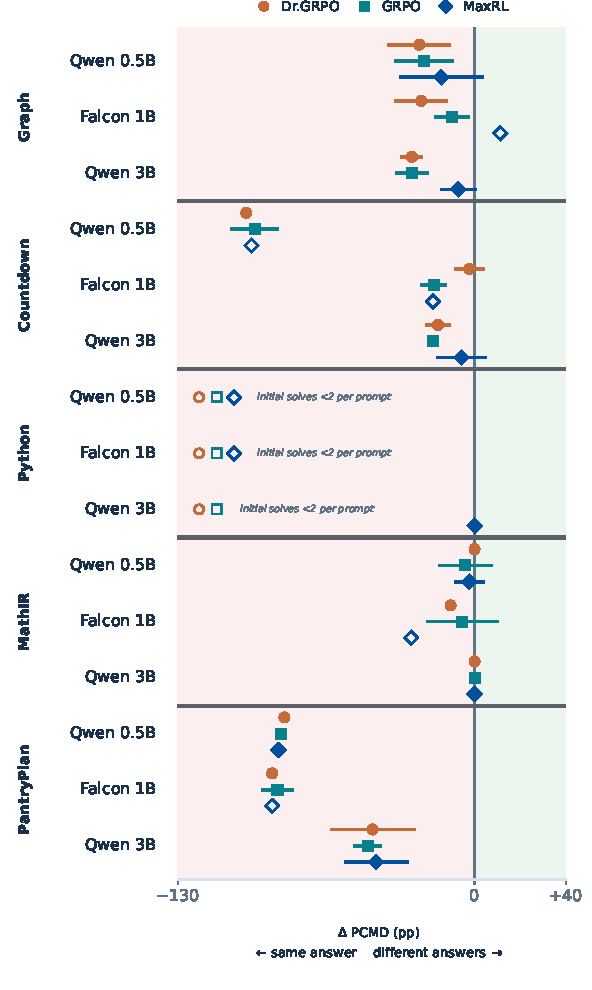
\includegraphics[width=\linewidth]{figures/concentration_story_all_scales.pdf}
  \end{minipage}\hfill
  \begin{minipage}[t]{.49\linewidth}
    \centering
    \textbf{(B)}\\[1pt]
    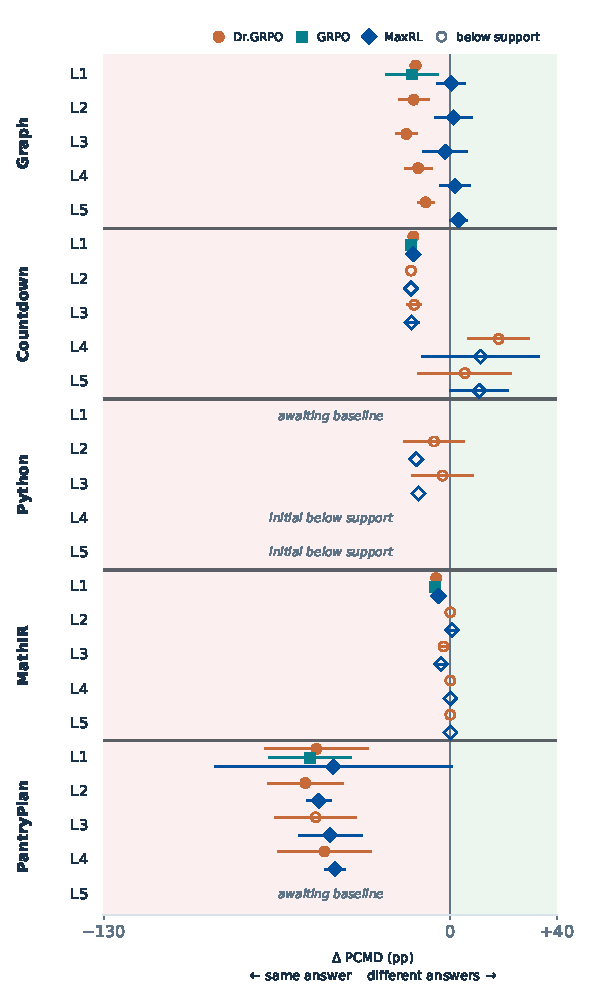
\includegraphics[width=\linewidth]{figures/concentration_levels.pdf}
  \end{minipage}
  \caption{\textbf{\texttt{Graph} and \texttt{PantryPlan} lose conditional solution diversity
  across scales and task levels.} Changes in \pmd{}, in percentage points.
  \textbf{(A)} Initial-to-final changes at Level~1 across three model scales
  and three objectives. Each seed averages over prompts with at least two
  correct responses at both checkpoints. Filled marks and bars show five-seed
  means and nominal paired 95\% Student-$t$ intervals. Open marks show
  means from fewer than five seeds, without intervals; annotated hollow
  symbols identify methods with no jointly eligible prompts. Dr.GRPO and GRPO reduce
  diversity in \texttt{Graph} and \texttt{PantryPlan} at every scale.
  \textbf{(B)} Level-1-trained policies evaluated on Levels~1--5, with
  Levels~2--5 measuring transfer. Available evaluations are averaged within
  each scale, then scales receive equal weight. Evaluations with different
  context limits contribute separately within a scale but do not constitute
  additional training seeds. Each scale uses one initial checkpoint evaluation.
  Bars appear only when one scale contributes and give nominal 95\%
  Student-$t$ intervals over its training seeds. Open marks indicate that at
  least one contributing scale has fewer than 30 eligible initial prompts or
  fewer than 30 eligible trained prompt observations in total. Missing initial
  references have fewer than two eligible prompts. GRPO appears only at
  Level~1. \texttt{Graph} and \texttt{PantryPlan} means decrease at every level; \texttt{Countdown}
  increases at Levels~4--5.}
  \label{fig:concentration-all-scales}
  \label{fig:concentration-levels}
\end{figure}


\subsection{Diversity before and after RLVR-only training}
\label{app:pre-rl-regression}

We evaluate Dr.GRPO and GRPO before training and after eight passes across
three models and five domains. The 150 runs each use four $K=8$ response
groups per checkpoint. Averaged equally across the five domains, extra
verified modes decrease by $98.2\%$--$99.4\%$ at Qwen2.5-0.5B and
$41.5\%$--$71.6\%$ at larger scales. The \texttt{pass@8} mean falls in
10 of the 30 domain--method--scale comparisons, while macro
\texttt{distinct@8} ends above its initial value at Qwen2.5-3B.
Fewer extra verified modes can therefore coexist with a greater probability
of sampling at least one correct response. Finite samples do not establish
that unobserved solution keys have zero probability.

\begin{samepage}
The domain average of \pmd{} includes only domains measurable at both endpoints: \texttt{Graph}, \texttt{MathIR}, and
\texttt{PantryPlan} at 0.5B; \texttt{Graph}, \texttt{Countdown}, and \texttt{PantryPlan} at 1B; and \texttt{Graph} and
\texttt{PantryPlan} at 3B. It declines by $98.5\%$ and $99.7\%$ at Qwen2.5-0.5B under
GRPO and Dr.GRPO, respectively, and by $50.8\%$--$65.1\%$ at the larger
scales. Terminal macro \pmd{} rounds to $.001$ for Dr.GRPO at Qwen2.5-0.5B.
The decline thus also appears in diversity conditional on success. Because
eligibility depends on the number of correct samples, these descriptive
averages do not hold the prompt population or correctness fixed.
App.~\ref{app:conditional-concentration} reports contrasts on jointly eligible
prompts. The decline is not universal: Falcon3-1B \texttt{Countdown} has
increasing \pmd{} under Dr.GRPO, from an initial value of $.033$.

\end{samepage}

Although the initial weights are shared, each method uses its own evaluation
samples. Differences between initial estimates therefore reflect sampling
variability.

\begin{figure}[t]
  \centering
  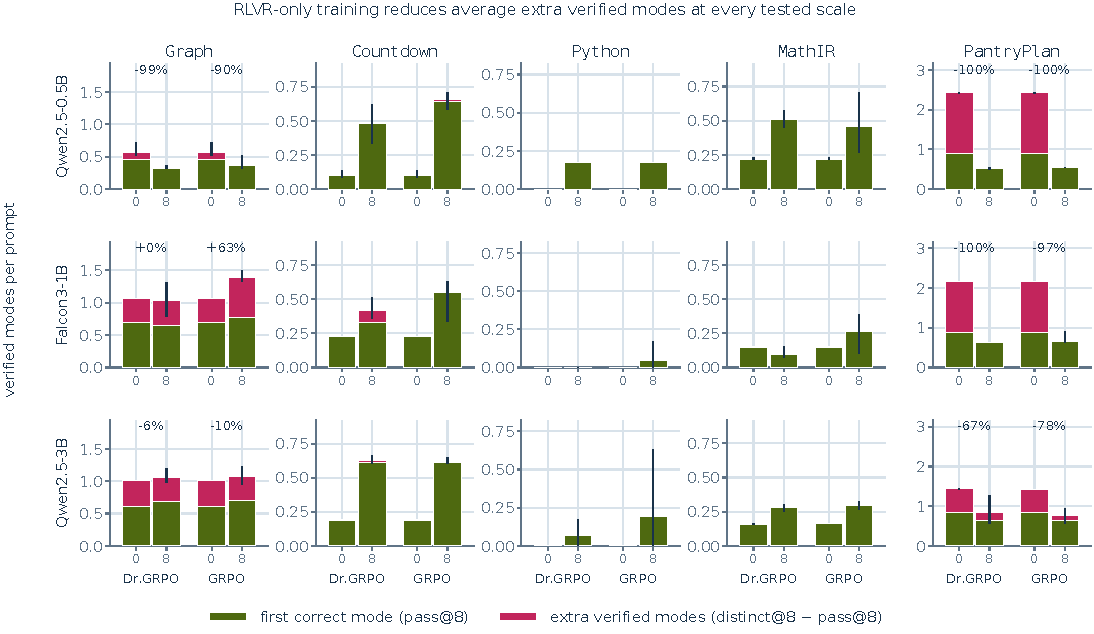
\includegraphics[width=\linewidth]{figures/baseline_collapse_precheck.pdf}
  \caption{\textbf{RLVR-only training reduces average extra verified modes
  at every tested scale.} Bars decompose \texttt{distinct@8} into
  \texttt{pass@8} and extra verified modes before training and after eight
  passes. Panels show Dr.GRPO and GRPO across three models and five domains:
  150 runs, with five seeds per model--domain--method combination and four
  eight-response groups per checkpoint. Whiskers show seed ranges; each
  method uses its own initial evaluation. Percentage changes in extra modes
  are shown for \texttt{Graph} and \texttt{PantryPlan}, whose initial means
  exceed $.05$. The other three domains start at $.011$ or less.}
  \label{fig:baseline-precheck}
\end{figure}




\texttt{Graph} and \texttt{PantryPlan} have substantial initial diversity at every
scale, whereas the other domains start with at most $.011$ extra modes per
prompt. To avoid unstable ratios near zero, retained-diversity percentages
are reported only when the initial extra-mode count exceeds $.05$.
The final $\texttt{distinct@8}$ is below its initial value in six of the
15 Dr.GRPO model--domain combinations. For Re:Dr, this occurs in two
available comparisons, both on \texttt{PantryPlan}; Falcon3-1B
\texttt{Countdown} uses four seeds. Conditional diversity comparisons
also depend on which prompts yield enough correct responses.
App.~\ref{app:conditional-concentration} reports paired contrasts on
jointly eligible prompts, including seed counts and uncertainty. These
held-out evaluations do not track individual modes stored during training.

Uniform sampling over the enumerable action representations gives a
diversity reference for \texttt{Graph} and \texttt{PantryPlan}
(App.~\ref{app:metric-sampling}). No corresponding reference is specified
for the other domains. On \texttt{PantryPlan}, uniform sampling of bit
masks yields higher expected \texttt{distinct@8} than the final sampled
value of every model under both Dr.GRPO and Re:Dr.

\begin{table}[t]
  \centering
  \caption{\textbf{Uniform actions and untrained checkpoints provide absolute diversity references.}
  \emph{Uniform} gives expected \distk{} under uniform sampling of the
  action representation: 27 color strings for \texttt{Graph} and 64 bit masks
  for \texttt{PantryPlan}. \emph{Initial} gives the Dr.GRPO pass-0 reference;
  the final two columns give sampled means after eight training passes.}
  \label{tab:absolute-support-references}
  \scriptsize
  \setlength{\tabcolsep}{4.2pt}
  \begin{tabular}{@{}llrrrr@{}}
    \toprule
    \textbf{Model} & \textbf{Domain} & \textbf{Uniform} & \textbf{Initial}
      & \textbf{Dr.GRPO} & \textbf{Re:Dr} \\
    \midrule
        \qwenmark{}2.5-0.5B & \texttt{Graph} & 1.633 & .561 & .325 & 2.438 \\
     & \texttt{PantryPlan} & 2.153 & 2.426 & .522 & 1.539 \\
    \addlinespace[2pt]
    Falcon3-1B & \texttt{Graph} & 1.633 & 1.070 & 1.034 & 1.717 \\
     & \texttt{PantryPlan} & 2.153 & 2.162 & .633 & 1.576 \\
    \addlinespace[2pt]
    \qwenmark{}2.5-3B & \texttt{Graph} & 1.633 & 1.012 & 1.060 & 1.637 \\
     & \texttt{PantryPlan} & 2.153 & 1.445 & .841 & 1.514 \\
    \bottomrule

  \end{tabular}
\end{table}


\subsection{Vanishing task gradients and repeated outputs}
\label{app:degenerate-groups}

A Dr.GRPO group with identical rewards has exactly zero fresh task gradient.
Only mixed groups, containing both correct and incorrect responses,
provide a nonzero task advantage. Optimizer momentum can still change the
policy when the current task gradient is zero. The table below reports
the fraction of mixed groups over 3,072 Qwen2.5-0.5B updates, averaged
across five seeds.

\begin{center}
\small
\begin{tabular}{@{}lrr@{}}
\toprule
\textbf{Domain} & \textbf{Dr.GRPO} & \textbf{Re:Dr} \\
\midrule
\texttt{Graph} & .144 & .954 \\
\texttt{Countdown} & .140 & .456 \\
\texttt{Python} & .015 & .185 \\
\texttt{MathIR} & .364 & .453 \\
\texttt{PantryPlan} & .123 & .789 \\
\bottomrule
\end{tabular}
\end{center}

Thus 98.5\% of \texttt{Python} control updates carry zero fresh task gradient.
Replay contributes a likelihood gradient from verified responses and can
also change the policy so that subsequent fresh groups contain both correct
and incorrect responses.

All five Qwen2.5-0.5B \texttt{Python} control seeds exhibit observed output collapse.
At pass 0, eight-response groups average 7.99 distinct completion strings
per prompt. By steps 288--480, all 32 temperature-1 responses for each
prompt are identical within each seed and match its greedy completion.
This holds on all 128 prompts and persists at every subsequent evaluation
through step 3,072. The 32 responses span four groups with overlapping sampling
streams (App.~\ref{app:conditional-concentration}); they are not 32 independent
draws. Within eight-response groups, the terminal mean is 1.00 distinct
completion per prompt for the control and 1.97 for replay. The repeated
completion can be incorrect. These finite observations do not rule out
low-probability alternatives.

This sparse binary-reward setting allows fresh task gradients to vanish.
Sampling strategies that favor mixed groups, larger groups, a reference-policy
KL penalty, token-entropy regularization, or broader decoding could change
this behavior. The present comparison does not isolate their effects.

\subsection{The controls learn at the fixed learning rates}
\label{app:control-learning-audit}

The controls use a constant learning rate of $2\times10^{-7}$ at
Qwen2.5-0.5B and Falcon3-1B and a peak rate of $10^{-7}$ with cosine decay
at Qwen2.5-3B (Table~\ref{tab:run-contract}). Learning rates are not swept.
Table~\ref{tab:control-learning-audit} reports changes in accuracy and the
frequency of informative response groups under these schedules. The
results characterize the tested settings without identifying an optimal
schedule for either method.

\begin{table}[t]
  \centering
  \caption{\textbf{Per-response accuracy increases in every control comparison,
  while \texttt{pass@8} can fall.} Accuracy compares initial and last
  available evaluations. Columns show unpaired five-run means for each
  model--domain combination. \texttt{mean@8} measures per-response
  correctness. Mixed gives the mean fraction of rollout groups
  containing both correct and incorrect responses. An unmixed group has
  zero fresh task advantage, although optimizer momentum can still change
  the policy. Training schedules match update counts and fresh-rollout
  budgets; total compute is discussed in App.~\ref{app:compute-accounting}.}
  \label{tab:control-learning-audit}
  \small
  \setlength{\tabcolsep}{5pt}
  \begin{tabular}{@{}llrrrrrrr@{}}
    \toprule
    & & \multicolumn{3}{c}{\textbf{control \texttt{pass@8}}}
      & \multicolumn{2}{c}{\textbf{control \texttt{mean@8}}}
      & \textbf{mixed} & \textbf{Re:Dr} \\
    \cmidrule(lr){3-5}\cmidrule(lr){6-7}
    \textbf{Model} & \textbf{Domain} & initial & terminal & $\Delta$
      & initial & terminal & groups & \texttt{pass@8} \\
    \midrule
    % Generated by ops/build_paper_control_learning_audit.py; do not hand edit.
    Qwen2.5-0.5B & \texttt{Graph} & .456 & .323 & $-$.132 & .178 & .323 & .144 & .969 \\
     & \texttt{Countdown} & .097 & .480 & $+$.383 & .014 & .465 & .140 & .672 \\
     & \texttt{Python} & .000 & .172 & $+$.172 & .000 & .172 & .015 & .528 \\
     & \texttt{MathIR} & .220 & .512 & $+$.292 & .037 & .464 & .364 & .796 \\
     & \texttt{PantryPlan} & .902 & .522 & $-$.380 & .344 & .522 & .123 & .729 \\
    \addlinespace[2pt]
    Falcon3-1B & \texttt{Graph} & .693 & .656 & $-$.037 & .178 & .300 & .777 & .809 \\
     & \texttt{Countdown} & .225 & .328 & $+$.103 & .037 & .268 & .400 & .636 \\
     & \texttt{Python} & .000 & .000 & $+$.000 & .000 & .000 & .009 & .979 \\
     & \texttt{MathIR} & .148 & .095 & $-$.053 & .023 & .068 & .158 & .736 \\
     & \texttt{PantryPlan} & .891 & .633 & $-$.258 & .318 & .633 & .523 & .751 \\
    \addlinespace[2pt]
    Qwen2.5-3B & \texttt{Graph} & .607 & .682 & $+$.075 & .215 & .360 & .706 & .836 \\
     & \texttt{Countdown} & .184 & .609 & $+$.426 & .049 & .569 & .281 & .746 \\
     & \texttt{Python} & .000 & .069 & $+$.069 & .000 & .069 & .011 & .659 \\
     & \texttt{MathIR} & .156 & .278 & $+$.122 & .061 & .168 & .152 & .686 \\
     & \texttt{PantryPlan} & .831 & .638 & $-$.193 & .267 & .558 & .482 & .744 \\
    \bottomrule

  \end{tabular}
\end{table}

\paragraph{Accuracy changes during training.}
Per-response correctness (\texttt{mean@8}) rises in all 15
control comparisons: every control learns under its schedule. What varies
is coverage. Using an absolute-change threshold of $.005$, 8 of the
15 comparisons improve in \texttt{pass@8} and
6 decline, so 7 controls gain per-response accuracy
without a \texttt{pass@8} increase above that threshold. The mean
\texttt{pass@8} change is +0.039; the largest increase is $+0.426$
(\texttt{Countdown} at Qwen2.5-3B) and the largest decrease is $-0.380$
(\texttt{PantryPlan} at Qwen2.5-0.5B). In \texttt{PantryPlan} at Falcon3-1B, per-response correctness rises from
0.318 to 0.633, while \texttt{pass@8}
falls from 0.891 to 0.633.
This combination is consistent with prior observations of increased
single-response accuracy alongside reduced sampling coverage
\citep{yue2025rlvrlimit}.

The gap between \texttt{pass@8} and \texttt{mean@8} is at least $.02$ in
12 initial model--domain comparisons and below $.02$ in
7 terminal comparisons. This gap reflects variation in
correctness within response groups; it does not identify repeated strings
or conditional diversity among correct solution keys. The completion-string
analysis in App.~\ref{app:degenerate-groups} directly measures repetition
for the Qwen2.5-0.5B \texttt{Python} controls.

\paragraph{Sparse fresh reward information.}
Initial \texttt{pass@8} is zero on \texttt{Python} at all three
scales. In \texttt{Python} at Falcon3-1B, only a fraction 0.009 of
updates contain mixed rewards, leaving zero fresh task advantage in
99.1\% of updates. A learning-rate change cannot make an
identically zero current task gradient nonzero, but it can change the effect
of informative updates, optimizer momentum, and subsequent sampling.
The Falcon3-1B \texttt{Python} control's terminal \texttt{pass@8} rounds to $.000$, while Re:Dr
ends at $.979$. This is an accuracy contrast in a sparse-success setting;
conditional mode diversity requires at least two correct responses per
prompt and is undefined when that sampling condition is unmet.

\paragraph{Scope of the comparison.}
Replay and control share the learning rate, schedule, initialization,
prompt stream, optimizer, update count, and fresh-rollout budget.
The comparison measures the effect of replay under these settings.
Per-response correctness increases in the controls, but the absence of a
learning-rate sweep limits conclusions about their optimal performance.
Other learning rates could change accuracy, diversity, and the relative
benefit of replay; the present results do not determine those changes.

The frequency of mixed groups helps characterize these comparisons.
When a control rarely produces mixed groups (App.~\ref{app:degenerate-groups}),
replay provides a likelihood gradient on updates with no fresh task advantage.
We therefore also summarize replay effects in subsets with increasing
control accuracy. Across all 15 model--domain combinations, the mean
Re:Dr minus Dr.GRPO effect is $+.352$ in \texttt{pass@8} and $+.189$
in \pmd{}. Among the 9 combinations with any positive initial-to-final
change in control \texttt{pass@8}, the effects are $+.379$ and $+.118$.
Among the 6 that also have nonzero initial \texttt{pass@8} and at least
10\% mixed rollout groups, they are $+.247$ and $+.136$. Every comparison
in these subsets has positive effects on both metrics; the smallest effects
in the six-comparison subset are $+.137$ in \texttt{pass@8} and $+.013$
in \pmd{}. Its mean diversity effect is about two thirds of the mean
across all comparisons. Table~\ref{tab:control-learning-audit} gives the
control measurements that define these subsets.

\subsection{Likelihood changes with a fixed replay buffer}
\label{app:fixed-bank-survival}

We examine the likelihoods of stored responses during Qwen2.5-0.5B Re:Dr
training on \texttt{Graph}, using five seeds. The buffer contents and counts
of fresh verified responses are held fixed from immediately before the
fresh rollout at step 384. Uniform replay continues through step 3,072
without adding modes. For each stored exemplar, identified by prompt and
canonical mode, we measure mean token log probability $s$ and sequence
log probability $\ell$ whenever it is replayed. Changes compare its first
and final replay visits after the buffer is fixed; these steps can differ
across exemplars.

The 3,406 exemplars span 1,575 seed--prompt pairs, with 8--9 replay visits
per exemplar.
The pooled median change is $+.038$ nat/token (95\% interval
$[+.025,+.048]$), while the 10th percentile is $-.256$ and $2.61\%$ of
exemplars lose more than $.5$ nat/token ($[1.54,3.77]\%$).
The largest observed intermediate decrease is $-1.328$ nat/token. Sequence log
probability has median change $+.154$ nat/sequence ($[+.104,+.198]$),
with $21.99\%$ of exemplars losing more than $.5$ nat/sequence.
Lengths range from 4 to 100 tokens, so the token and sequence thresholds
measure different changes.

\begin{figure}[!htbp]
  \centering
  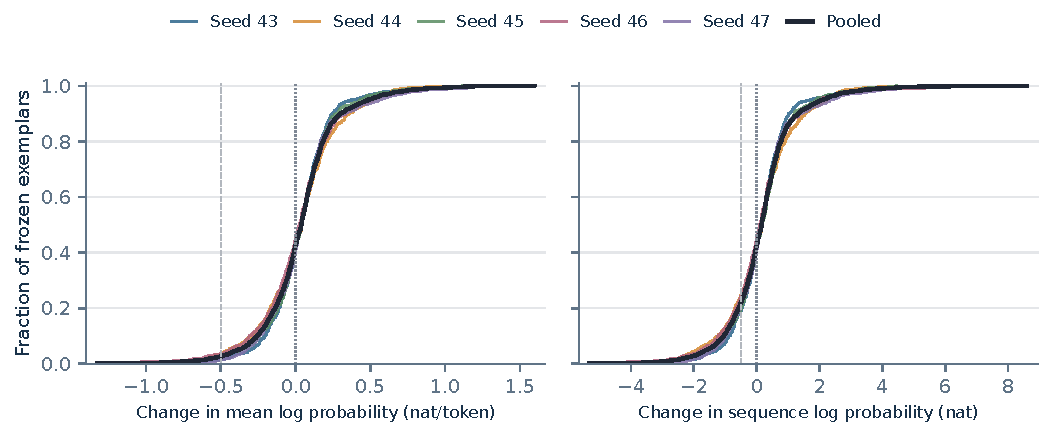
\includegraphics[width=.95\linewidth]{figures/e121_fixed_bank_survival.pdf}
  \caption{\textbf{Median exemplar scores rise, while some exemplars decline.}
  Empirical cumulative distributions of first-to-final score changes for
  3,406 fixed-buffer exemplars from five Qwen2.5-0.5B Re:Dr \texttt{Graph} seeds.
  Panels show mean token and sequence log probability. Colored curves
  represent individual seeds; the pooled curve weights exemplars equally.
  Dotted and dashed vertical lines mark zero and $-.5$, respectively.
  Positive changes indicate higher likelihood for the stored token sequence.
  Sequence likelihood does not measure the total probability of generating
  a canonical solution mode.}
  \label{fig:e121-fixed-bank-survival}
\end{figure}

Pooled summaries weight exemplars equally. Descriptive 95\% percentile
intervals use 10,000 hierarchical bootstrap replicates, resampling prompts
with replacement within each training seed and then resampling the five
seeds with replacement.

Scores are measured at replay visits, so changes between visits are
unobserved. Some stored exemplars lose likelihood despite continued replay.
A matched fixed-buffer control without replay would be needed to isolate
the effect of replay. These sequence-level observations also do not test
the mode-probability floor in Theorem~\ref{thm:replay-retention}.

\clearpage
\phantomsection
\begin{center}\large\textbf{Part IV. What diversity represents}\end{center}
\addcontentsline{toc}{part}{Part IV. What diversity represents}

\section{Matched Prompt-Hint Ablation}
\label{app:prompt-hint-ablation}

\subsection{Removing strategy hints from unchanged problems}

\label{sec:prompt-hint-ablation}

We compare original and neutral prompts on \texttt{Python}, \texttt{MathIR}, and \texttt{PantryPlan} at Levels 2 and 3. Each of the six domain--level combinations uses 32 problems selected independently of model outputs from the 128-problem evaluation split. We sample eight responses per problem under each wording. The original wording uses the standard prompt. The neutral wording removes the \texttt{Python} nested-conditional example and suggestions to test small divisors or dispatch on listed values, the \texttt{MathIR} ordered algebraic-isolation suggestion, and the \texttt{PantryPlan} preference for ingredients high in energy and protein but low in sodium such as seeds or oats. \texttt{MathIR} changes ``those operations'' to ``the operations'' to preserve the instruction to return a menu ID. The problem instance, answer specification, executable verifier, and remaining format requirements are unchanged.

The paired effects are neutral minus original on empirical $P_8=\texttt{pass@8}$ and $D_8=\texttt{distinct@8}$, with $B_8=D_8-P_8$ as extra verified modes per problem. Incorrect, empty, and truncated outputs remain in their eight-draw groups; only verifier-accepted outputs contribute a verified key. Results use strict verification. A sensitivity analysis with normalized formatting preserves every strict success and canonical key and applies the same rules to both arms.

Intervals use 20,000 whole-problem bootstrap resamples, paired across arms and stratified by domain and level. Domain--level combinations receive equal weight in aggregate estimates. The intervals are pointwise 95\% percentile intervals without multiplicity adjustment. With 32 problems per domain and level, an interval crossing zero does not establish equivalence. A zero-width interval reflects zero variation in the observed bootstrap resamples, including identical paired $P_8$ outcomes, and does not establish population equivalence. Correct-pair collision and its certified-support uniform reference use the same correct-pair weights. Eight draws per prompt do not identify total unseen support.



We evaluate the initial Qwen2.5-0.5B-Instruct checkpoint and Level-2-trained Dr.GRPO and Re:Dr checkpoints. \texttt{Python} and \texttt{MathIR} use five matched training seeds; \texttt{PantryPlan} uses two. Level 3 tests transfer from Level 2 training. All checkpoints evaluate the same selected problems under the benchmark syntax constraints and a 192-token generation budget. Five-seed intervals resample whole training seeds and paired problems; \texttt{PantryPlan} intervals condition on its two checkpoints, and initial-model intervals condition on one instruction-tuned checkpoint. These effects concern the specified models, problems, and interface.


\begin{table}[t]
\centering
\scriptsize
\setlength{\tabcolsep}{2.2pt}
\caption{\textbf{Removing \texttt{Python} guidance reduces correctness and observed breadth.} Qwen2.5-0.5B checkpoints under strict verification, with original $\to$ neutral wording. $P_8=\texttt{pass@8}$, $D_8=\texttt{distinct@8}$, and $B_8=D_8-P_8$ use eight draws on each of 32 problems per domain and level. Effects are neutral minus original. $P_8$, $D_8$, and $B_8$ average the displayed number $s$ of checkpoints. Brackets are pointwise 95\% bootstrap intervals: paired problems and training seeds are resampled for five-seed groups; \texttt{PantryPlan} intervals condition on its two checkpoints, and initial-model intervals on one checkpoint. \pmd{} estimates the probability that two correct responses have different canonical keys, averaging checkpoint--problem groups with at least two verified draws in each arm. Its paired population depends on correctness, and repeated problems at different checkpoints count separately. Only 5 of 18 comparisons meet the minimum of 30 such groups; dashes denote the others. These \pmd{} point estimates have no reported uncertainty intervals.}
\label{tab:prompt-hints-local-strict}
\resizebox{\linewidth}{!}{%
\begin{tabular}{llrrrrrrr}
\toprule
Model & Domain/level & $P_8$: O$\to$N & $D_8$: O$\to$N & $\Delta P_8$ [95\%] & $\Delta D_8$ [95\%] & $\Delta B_8$ & \pmd{}: O$\to$N & $\Delta$ \pmd{} \\
\midrule
Initial ($s=1$) & \texttt{Python} L2 & $0.656\to0.125$ & $0.69\to0.12$ & $-0.531\;[-0.719,-0.344]$ & $-0.56\;[-0.75,-0.38]$ & $-0.03$ & -- & -- \\
Initial ($s=1$) & \texttt{MathIR} L2 & $0.250\to0.281$ & $0.25\to0.28$ & $+0.031\;[+0.000,+0.094]$ & $+0.03\;[+0.00,+0.09]$ & $+0.00$ & -- & -- \\
Initial ($s=1$) & \texttt{PantryPlan} L2 & $0.156\to0.188$ & $0.19\to0.22$ & $+0.031\;[+0.000,+0.094]$ & $+0.03\;[+0.00,+0.09]$ & $+0.00$ & -- & -- \\
Initial ($s=1$) & \texttt{Python} L3 & $0.719\to0.031$ & $0.81\to0.03$ & $-0.688\;[-0.844,-0.531]$ & $-0.78\;[-0.97,-0.59]$ & $-0.09$ & -- & -- \\
Initial ($s=1$) & \texttt{MathIR} L3 & $0.219\to0.219$ & $0.22\to0.22$ & $+0.000\;[-0.125,+0.125]$ & $+0.00\;[-0.12,+0.12]$ & $+0.00$ & -- & -- \\
Initial ($s=1$) & \texttt{PantryPlan} L3 & $0.281\to0.312$ & $0.66\to0.69$ & $+0.031\;[+0.000,+0.094]$ & $+0.03\;[-0.06,+0.12]$ & $+0.00$ & -- & -- \\
Dr.GRPO ($s=5$) & \texttt{MathIR} L2 & $0.531\to0.506$ & $0.53\to0.51$ & $-0.025\;[-0.100,+0.031]$ & $-0.03\;[-0.10,+0.03]$ & $+0.00$ & $.000\to.000$ & $+.000$ \\
Dr.GRPO ($s=5$) & \texttt{MathIR} L3 & $0.194\to0.156$ & $0.19\to0.16$ & $-0.037\;[-0.113,+0.019]$ & $-0.04\;[-0.11,+0.02]$ & $+0.00$ & -- & -- \\
Dr.GRPO ($s=2$) & \texttt{PantryPlan} L2 & $0.219\to0.203$ & $0.28\to0.25$ & $-0.016\;[-0.156,+0.125]$ & $-0.03\;[-0.19,+0.12]$ & $-0.02$ & -- & -- \\
Dr.GRPO ($s=2$) & \texttt{PantryPlan} L3 & $0.172\to0.172$ & $0.27\to0.25$ & $+0.000\;[-0.078,+0.078]$ & $-0.02\;[-0.16,+0.11]$ & $-0.02$ & -- & -- \\
Dr.GRPO ($s=5$) & \texttt{Python} L2 & $0.812\to0.000$ & $0.81\to0.00$ & $-0.812\;[-0.938,-0.656]$ & $-0.81\;[-0.94,-0.66]$ & $+0.00$ & -- & -- \\
Dr.GRPO ($s=5$) & \texttt{Python} L3 & $1.000\to0.000$ & $1.00\to0.00$ & $-1.000\;[-1.000,-1.000]$ & $-1.00\;[-1.00,-1.00]$ & $+0.00$ & -- & -- \\
Re:Dr ($s=5$) & \texttt{MathIR} L2 & $0.994\to0.975$ & $0.99\to0.97$ & $-0.019\;[-0.075,+0.000]$ & $-0.02\;[-0.07,+0.00]$ & $+0.00$ & $.000\to.000$ & $+.000$ \\
Re:Dr ($s=5$) & \texttt{MathIR} L3 & $0.312\to0.275$ & $0.31\to0.28$ & $-0.037\;[-0.138,+0.044]$ & $-0.04\;[-0.14,+0.04]$ & $+0.00$ & $.000\to.000$ & $+.000$ \\
Re:Dr ($s=2$) & \texttt{PantryPlan} L2 & $0.516\to0.500$ & $0.75\to0.73$ & $-0.016\;[-0.109,+0.078]$ & $-0.02\;[-0.20,+0.17]$ & $+0.00$ & -- & -- \\
Re:Dr ($s=2$) & \texttt{PantryPlan} L3 & $0.234\to0.281$ & $0.39\to0.50$ & $+0.047\;[+0.000,+0.109]$ & $+0.11\;[+0.05,+0.19]$ & $+0.06$ & -- & -- \\
Re:Dr ($s=5$) & \texttt{Python} L2 & $0.887\to0.556$ & $1.24\to0.68$ & $-0.331\;[-0.525,-0.150]$ & $-0.57\;[-0.85,-0.32]$ & $-0.24$ & $.231\to.173$ & $-.058$ \\
Re:Dr ($s=5$) & \texttt{Python} L3 & $1.000\to0.494$ & $1.42\to0.66$ & $-0.506\;[-0.825,-0.194]$ & $-0.76\;[-1.07,-0.38]$ & $-0.26$ & $.256\to.323$ & $+.067$ \\
\bottomrule
\end{tabular}}
\end{table}


\pmd{} is reported for five of the 18 comparisons in Table~\ref{tab:prompt-hints-local-strict}. Each requires at least thirty checkpoint--problem groups with at least two verified draws under each wording. The same 32 problems are evaluated at each checkpoint, so these group counts include repeated problems across training seeds. Within a comparison, \pmd{} weights eligible groups equally; checkpoints with more eligible problems therefore receive more weight. The population depends on success under both wordings and need not represent all evaluated problems. Three eligible comparisons are \texttt{MathIR}: all observed verified pairs within each eligible group share a canonical key, giving \pmd{} $=.000$ under both wordings. This observation does not limit the number of valid keys. In the two Re:Dr comparisons on \texttt{Python}, hint removal changes \pmd{} from $.231$ to $.173$ at Level 2 and from $.256$ to $.323$ at Level 3, on 66 and 57 eligible checkpoint--problem groups, respectively. The two point estimates have opposite signs; without intervals, they do not establish a shared direction or the reliability of either concentration effect. At Level 3, conditional diversity uses four training seeds, while $P_8$ and $D_8$ use all five; the fifth seed has too few jointly verified responses. A dash denotes an unavailable conditional estimate, not a zero effect.


Formatting normalization adds no verified responses for any Qwen2.5-0.5B checkpoint in this panel; all tabulated estimates and intervals therefore agree under the two grading rules.


\begin{figure}[t]

\centering

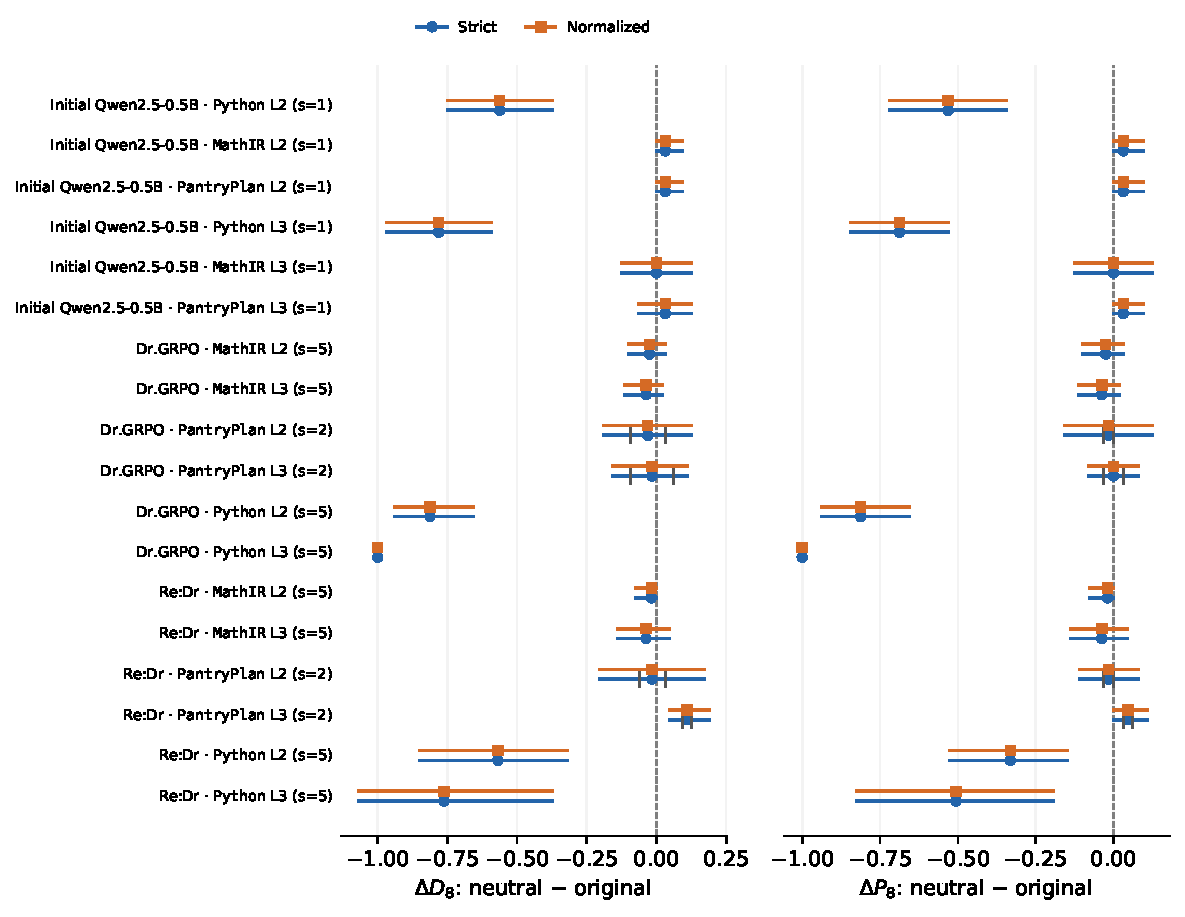
\includegraphics[width=\linewidth]{figures/modebench_prompt_ablation_local.pdf}

\caption{\textbf{\texttt{Python} guidance removal produces the largest wording effects in this panel.} Neutral-minus-original $D_8$ (left) and $P_8$ (right) for the initial Qwen2.5-0.5B checkpoint and Level-2-trained Dr.GRPO and Re:Dr on \texttt{Python}, \texttt{MathIR}, and \texttt{PantryPlan} at Levels 2 and 3, with 32 paired problems and eight draws per arm. Blue circles use strict verification; orange squares use formatting normalization. Horizontal bars are pointwise 95\% bootstrap intervals; the vertical dashed line marks zero. Five-seed groups resample training seeds and paired problems; \texttt{PantryPlan} and initial-model intervals condition on two checkpoints and one checkpoint, respectively. Gray marks show the individual effects for the two \texttt{PantryPlan} training seeds. }

\label{fig:prompt-hints-local}

\end{figure}



\begin{samepage}
\paragraph{Two-seed \texttt{PantryPlan} effects.} Intervals condition on the two checkpoints and do not quantify training-seed variability. The effects for each seed are shown below; each pair gives $(\Delta P_8,\Delta D_8)$.
\begin{center}\small
\begin{tabular}{llcc}
\toprule
Method & Level & First seed & Second seed \\
\midrule
Dr.GRPO & 2 & $(+0.000, +0.03)$ & $(-0.031, -0.09)$ \\
Dr.GRPO & 3 & $(+0.031, +0.06)$ & $(-0.031, -0.09)$ \\
Re:Dr & 2 & $(-0.031, -0.06)$ & $(+0.000, +0.03)$ \\
Re:Dr & 3 & $(+0.031, +0.12)$ & $(+0.062, +0.09)$ \\
\bottomrule
\end{tabular}
\end{center}
\end{samepage}

\paragraph{Scope of the wording intervention.}
The \texttt{Python} intervention removes an executable nested-conditional example
along with divisor-testing and dispatch guidance, and it shortens the prompt.
Its effect concerns this combined change; it does not isolate a preference
cue from example or length effects. Lower \texttt{distinct@8} together with
lower \texttt{pass@8} can reflect reduced correctness rather than increased
concentration among correct outputs. The \pmd{} columns in
Table~\ref{tab:prompt-hints-local-strict} measure conditional diversity on
jointly eligible checkpoint--problem groups. Eligibility itself depends on
correctness, so these comparisons do not hold the full evaluation population
or its accuracy fixed.

\paragraph{Observed prompt dependence.}
\texttt{Python} shows a large loss of correctness after guidance removal. Across the
five Dr.GRPO seeds, mean $P_8$ falls from $.8125$ to zero at Level~2 and from
$1.0$ to zero at Level~3; $D_8$ falls identically and $B_8=0$ in both arms.
With no correct neutral Dr.GRPO outputs, its concentration among correct outputs
is undefined. Re:Dr retains neutral $P_8=.55625$ and $.49375$ and
$D_8=.675$ and $.65625$ at Levels~2 and~3, respectively, while losing
extra verified modes: $\Delta B_8=-.2375$ and $-.25625$. The initial checkpoint
also loses \texttt{Python} correctness (Table~\ref{tab:prompt-hints-local-strict}).
These observations identify substantial dependence on the combined \texttt{Python}
wording intervention; a raw mode-count decline cannot be interpreted solely
as a redistribution among correct answers.


\paragraph{\texttt{Python} responses after hint removal.}
Across 5,120 Dr.GRPO \texttt{Python} responses from five seeds, two levels, and both
wordings, all 2,560 outputs generated with the original wording yield the
same extracted lambda expression, whose body matches the conditional
example in the prompt; 2,320 of these
responses pass verification:
\begin{quote}\footnotesize\ttfamily
lambda n: 2 if n \% 2 == 0 else 3 if n \% 3 == 0 else 5
\end{quote}
\begin{samepage}
Of the 2,560 neutral-wording responses, 1,816 (70.94\%) are invalid Python
expressions, 59 violate other restricted-language rules, 376 return
non-integers, 276 fail the proper-divisor condition, and 33 (1.29\%) have
no extracted candidate after reaching the token limit. Syntax errors are
the largest failure category. The categories follow the first rejection
during extraction, parsing, and execution. They describe output failures
without identifying the training mechanism responsible.

\end{samepage}

\paragraph{Concentration after hint removal.}
Every trained \texttt{MathIR} checkpoint has $B_8=0$ under both wordings at both levels.
Within each problem's eight-draw group, every observed pair of correct
outputs shares a canonical key at every trained checkpoint and level:
correct-pair collision is $1.0$, versus the
uniform reference of $.2$ over five certified modes.
Table~\ref{tab:prompt-hints-local-strict} reports \pmd{} $.000$ under both
wordings in every eligible \texttt{MathIR} comparison. Removing this hint therefore leaves
observed correct outputs concentrated. At Level~2, Re:Dr retains mean $P_8=.975$ without the order hint, compared with $.99375$
with it. Across its five checkpoints, the neutral arm has 4,179 colliding
pairs out of 4,179 correct pairs, from 154 eligible checkpoint--problem
groups; the original arm has 4,382 out of 4,382 pairs from 157 such groups.
Both arms evaluate the same 32 problems at each checkpoint. Thus observed concentration persists after removing the order hint.
The comparison does not measure unseen modes, and the remaining interface
constraints still apply.
\texttt{PantryPlan} effects are mixed. Re:Dr at Level~3 gains $.109375$ in $D_8$,
comprising $.046875$ in $P_8$ and $.0625$ in $B_8$, but this comparison has only
two training seeds. App.~\ref{app:sampling-budget-ablation} evaluates
hosted models under both wordings with 64 draws on sixteen problems per
domain--level combination. Its problem population and sampling budget
differ from the eight-draw evaluation here.


\section{Decoding Temperature, Nucleus, and Budget}
\label{app:decoding-objection}

\paragraph{Temperature at fixed checkpoints.}
Qwen2.5-0.5B Dr.GRPO and Re:Dr checkpoints after eight training passes are
evaluated at $T\in\{.5,.7,1.0,1.3,1.6,2.0\}$, with top-$p=1$ and four
eight-response groups per prompt. Five domains, two methods, and five seeds
give 300 checkpoint--setting evaluations (Fig.~\ref{fig:decoding-objection}A).
The prompt template, evaluation split, response limit, and sampling seeds
are fixed across temperatures. Correct keys are pooled across response
groups for each prompt; the groups have overlapping sampling streams
(App.~\ref{app:conditional-concentration}). Estimates therefore describe
these sampled pools. A seed contributes to the \pmd{} mean when at least
30 prompts yield at least two correct responses. Eligible prompts and seeds
can differ across temperatures and methods.

Across the six temperatures, the largest control \pmd{} is $.021$ in
\texttt{Graph}, $.016$ in \texttt{Countdown}, $.002$ in \texttt{MathIR}, and $.004$ in \texttt{PantryPlan}.
Re:Dr at $T=1$ has corresponding means $.562$, $.485$, $.020$, and $.330$.
These four domains retain five eligible control seeds at every temperature.
\texttt{Python} controls have no seed reaching the 30-prompt threshold, so their
conditional diversity is unidentified under this reporting rule.
The sweep therefore shows low measured control diversity in the four
eligible domains, without establishing that unobserved modes have zero
probability or that every decoding choice would behave the same way.

\paragraph{Hardware sensitivity.}
All evaluations in the temperature sweep use NVIDIA RTX A5000 GPUs.
A paired comparison of A100 and A5000 evaluations at $T=1$ gives mean
absolute \pmd{} difference $.0032$ across twelve comparisons, with maximum
$.0131$. These differences describe the tested hardware comparisons;
they do not bound hardware sensitivity at other checkpoints or settings.

\paragraph{Larger groups and nucleus truncation.}
A separate set of Qwen2.5-0.5B checkpoints trained for twelve passes is evaluated at
eleven settings (Fig.~\ref{fig:decoding-objection}B): the six temperatures
above; two groups of $K=32$ at $T\in\{1.0,1.3,1.6\}$; and four groups
of $K=8$ with top-$p=.95$ at $T\in\{1.0,1.6\}$. The $K=32$ settings
quadruple the group size and double total responses per prompt from 32 to
64. Five domains, two methods, and five seeds give 550 checkpoint--setting
evaluations. The replay variant combines separate mass and within-buffer
balancing terms with novelty and semantic-entropy shaping. Its objective
and training duration therefore differ from the eight-pass Re:Dr comparison.

Control \pmd{} is zero throughout the grid in \texttt{Graph}. Its range is $.006$
to $.031$ in \texttt{Countdown}, $.000$ to $.003$ in \texttt{MathIR}, and $.037$ to $.069$
in \texttt{PantryPlan}.
All eleven settings retain five eligible control seeds in these domains;
\texttt{Python} controls remain below the reporting threshold. The replay markers
provide a descriptive reference for this separate variant, without
identifying the effect of the Re:Dr objective.

Three comparisons hold temperature and nucleus sampling fixed while
increasing both group size and total response budget: $K=8$ and $K=32$ at
$T\in\{1.0,1.3,1.6\}$, top-$p=1$. Across these matched settings, control
\pmd{} changes by at most $.010$ in absolute value, and no
$K=32$ control mean exceeds $.054$. \texttt{Graph} stays at $.000$;
\texttt{Countdown} moves from $.014$--$.027$ to $.013$--$.023$;
\texttt{MathIR} from $.000$--$.001$ to $.001$--$.003$; and \texttt{PantryPlan}
from $.050$--$.063$ to $.045$--$.053$. Each mean uses five eligible seeds.
The larger budget therefore does not move these controls out of their
low-\pmd{} range. This compares sampled pools at fixed checkpoints; it does
not establish that unobserved modes carry zero probability.

\begin{figure}[t]
  \centering
  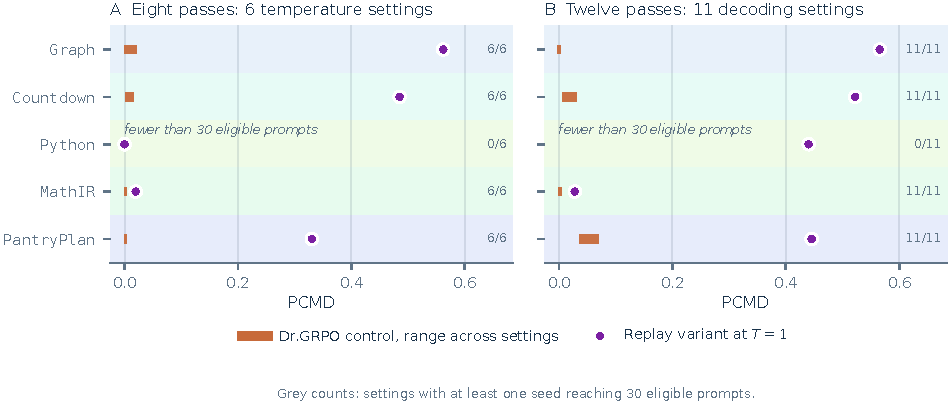
\includegraphics[width=\linewidth]{figures/decoding_objection.pdf}
  \caption{\textbf{Control diversity remains low across the tested decoding
  settings.} Qwen2.5-0.5B terminal \pmd{} across five domains.
  \textbf{(A)} Eight-pass Dr.GRPO/Re:Dr checkpoints at six temperatures
  ($T=.5$--$2.0$): 300 checkpoint--setting evaluations.
  \textbf{(B)} Separate twelve-pass checkpoints at eleven temperature, group-size,
  and nucleus settings: 550 evaluations, using a different replay objective.
  Bars span control means across settings; they are not confidence intervals.
  Markers show the corresponding replay variant at $T=1$, top-$p=1$,
  and $K=8$. Means use seeds with at least 30 prompts having at least two correct
  responses, so control and replay populations need not match. Control bars
  use five seeds outside \texttt{Python}; \texttt{Python} controls have none, while its replay
  markers use two seeds in A and three in B. Counts give eligible settings.
  Ranges narrower than $.004$ are displayed at width $.004$ for visibility.}
  \label{fig:decoding-objection}
\end{figure}

\paragraph{Scope of the decoding comparison.}
Both grids evaluate fixed terminal policies at one model scale. They do not
measure the effects of changing rollout temperature, optimizer settings, or
training duration. Correctness and conditional eligibility can change with
decoding settings; a missing \pmd{} estimate indicates insufficient eligible
prompts, rather than disappearance of all correct solution modes.

\section{Sampling-Budget Ablation}
\label{app:sampling-budget-ablation}

\subsection{Sampling design and estimands}
\label{sec:discovery-curves}
Large-budget \texttt{pass@k} evaluation can reveal differences hidden at smaller budgets \citep{yue2025rlvrlimit}. We evaluate sixteen problems from each of \texttt{Python}, \texttt{MathIR}, and \texttt{PantryPlan} at Levels~2 and~3.

Problems are selected independently of model outputs from the prompt-hint ablation population. Each has original and neutral wordings, with 64 responses per wording from each checkpoint or deployment. Eight-draw estimates use subsets of these same response pools. The initial Qwen2.5-0.5B-Instruct checkpoint has no training-seed replication. Dr.GRPO and Re:Dr use five matched seeds in \texttt{Python} and \texttt{MathIR} and two in \texttt{PantryPlan}. These checkpoints are trained at Level~2, so Level~3 measures transfer.

For a 64-draw pool, let $c$ be the number of correct outputs and $n_j$ the count of verified canonical key $j$. At $k\in\{1,2,4,8,16,32,64\}$, we average over all size-$k$ subsets without replacement:
\[
 P_k=1-\frac{\binom{64-c}{k}}{\binom{64}{k}},\qquad
 D_k=\sum_j\left[1-\frac{\binom{64-n_j}{k}}{\binom{64}{k}}\right],\qquad B_k=D_k-P_k.
\]
Here $P_k$ is the probability of at least one correct response, $D_k$ is the expected number of distinct verified modes, and $B_k$ is the expected number of modes beyond the first success. Infeasible numerator combinations are zero. Incorrect, empty, refused, and truncated responses remain in the pool; only verifier-accepted responses contribute keys. The curve points are correlated because they share a response pool and describe finite-sample discovery. The gains $G_P=P_{64}-P_8$, $G_D=D_{64}-D_8$, and $G_B=B_{64}-B_8$ distinguish improvements in first-success probability from the discovery of additional modes; they do not estimate complete unseen support.

We report strict-verifier results and a formatting-normalization sensitivity analysis that preserves every strict success and canonical key. Intervals use 20,000 whole-problem bootstrap replicates, paired across wordings and stratified by domain and level. Five-seed intervals also resample matched training seeds with shared problem indices; \texttt{PantryPlan} intervals condition on its two checkpoints. Each domain--level comparison contains sixteen problems, and intervals are unadjusted for multiple comparisons. Zero-width intervals indicate no observed resampled variation and do not establish equivalence.

For breadth at a fixed number of correct draws, we average over subsets of $m$ correct responses:
\[
 R_m=\sum_j\left[1-\frac{\binom{c-n_j}{m}}{\binom{c}{m}}\right].
\]
Paired comparisons require $c\ge m$ under both wordings. They therefore condition on observed success, without equating accuracy or estimating diversity for excluded problems.

Eligibility varies with $m$, method, and grading. Trained-checkpoint means weight seeds equally and are undefined if any seed lacks eligible prompts. Conditional intervals retain only bootstrap replicates in which the corresponding mean is defined.

The 64-draw summaries use two prompt weightings. Pooled collision $C$ divides the total number of equal-key correct pairs by the total number of correct pairs within each checkpoint or deployment; a prompt therefore receives weight proportional to $\binom{c}{2}$. Promptwise \pmd{} averages $1-\sum_j\binom{n_j}{2}/\binom{c}{2}$ equally over prompts with $c\ge2$. Each wording's absolute estimate uses its own eligible prompts, whereas the neutral-minus-original contrast $\Delta\pmd$ uses only jointly eligible prompts. Trained-checkpoint estimates then receive equal weight across seeds.

Support references use certified lower bounds $L\le M$: two valid modes in \texttt{Python}, five in \texttt{MathIR}, and the problem-specific certificate count in \texttt{PantryPlan}. Thus $1/L$ is an upper reference for collision under a uniform distribution over full support, and $L[1-(1-1/L)^m]$ is a lower reference for uniform expected breadth. These references describe uniform sampling; they do not bound model breadth, and observed distinct counts may exceed $L$.

In the tables, O/N denotes original/neutral wording, and $\Delta G_D$ is the neutral-minus-original discovery gain. $U$ denotes the uniform reference under the corresponding weighting. $E_O/E_N$ count separately eligible checkpoint--problem pairs with $c\ge2$; $Q_O/Q_N$ count correct response pairs. The counts sum across checkpoints, whereas the estimates weight checkpoints equally. Separate eligibility counts do not give the size of the jointly eligible population used for a contrast.


\begin{table}[!htbp]
\centering\scriptsize
\setlength{\tabcolsep}{3pt}
\caption{\textbf{Discovery gains from eight to 64 draws.} Strict verification; O/N denotes original/neutral wording. Each row reports sixteen problems for one deployment, domain, and level. Intervals resample paired problems, with no replication across model training seeds.}
\label{tab:discovery-gains-frontier-strict}
\resizebox{\linewidth}{!}{%
\begin{tabular}{llrrrr}
\toprule
Model & Domain/level & $G_P$: O/N & $G_D$: O/N & $G_B$: O/N & $\Delta G_D$ [95\%] \\
\midrule
GPT-5.4 & \texttt{Python} L2 & $0.014/0.000$ & $2.017/3.051$ & $2.003/3.051$ & $+1.033\;[-0.044,+2.371]$ \\
GPT-5.6 Sol & \texttt{Python} L2 & $0.000/0.405$ & $0.000/0.866$ & $0.000/0.462$ & $+0.866\;[+0.545,+1.231]$ \\
Grok 4.3 & \texttt{Python} L2 & $0.000/0.000$ & $0.667/1.013$ & $0.667/1.013$ & $+0.346\;[-0.583,+1.128]$ \\
GPT-5.4 & \texttt{Python} L3 & $0.025/0.000$ & $2.100/2.340$ & $2.076/2.340$ & $+0.240\;[-0.379,+0.930]$ \\
GPT-5.6 Sol & \texttt{Python} L3 & $0.000/0.586$ & $0.000/0.759$ & $0.000/0.174$ & $+0.759\;[+0.581,+0.952]$ \\
Grok 4.3 & \texttt{Python} L3 & $0.000/0.000$ & $0.424/1.576$ & $0.424/1.576$ & $+1.152\;[+0.640,+1.689]$ \\
GPT-5.4 & \texttt{MathIR} L2 & $0.043/0.042$ & $0.043/0.909$ & $0.000/0.868$ & $+0.867\;[+0.587,+1.111]$ \\
GPT-5.6 Sol & \texttt{MathIR} L2 & $0.027/0.004$ & $0.027/0.686$ & $0.000/0.682$ & $+0.659\;[+0.416,+0.888]$ \\
Grok 4.3 & \texttt{MathIR} L2 & $0.000/0.001$ & $0.223/0.322$ & $0.223/0.321$ & $+0.099\;[-0.226,+0.438]$ \\
GPT-5.4 & \texttt{MathIR} L3 & $0.000/0.000$ & $0.055/0.663$ & $0.055/0.663$ & $+0.609\;[+0.342,+0.888]$ \\
GPT-5.6 Sol & \texttt{MathIR} L3 & $0.000/0.000$ & $0.000/0.515$ & $0.000/0.515$ & $+0.515\;[+0.318,+0.714]$ \\
Grok 4.3 & \texttt{MathIR} L3 & $0.000/0.000$ & $0.167/0.805$ & $0.167/0.805$ & $+0.638\;[+0.348,+0.935]$ \\
GPT-5.4 & \texttt{PantryPlan} L2 & $0.001/0.015$ & $1.158/2.583$ & $1.156/2.568$ & $+1.426\;[+0.423,+2.641]$ \\
GPT-5.6 Sol & \texttt{PantryPlan} L2 & $0.086/0.101$ & $0.917/1.789$ & $0.831/1.688$ & $+0.872\;[+0.245,+1.575]$ \\
Grok 4.3 & \texttt{PantryPlan} L2 & $0.000/0.000$ & $1.022/3.377$ & $1.022/3.377$ & $+2.354\;[+1.592,+3.123]$ \\
GPT-5.4 & \texttt{PantryPlan} L3 & $0.000/0.002$ & $1.666/3.219$ & $1.666/3.218$ & $+1.553\;[+0.776,+2.367]$ \\
GPT-5.6 Sol & \texttt{PantryPlan} L3 & $0.032/0.129$ & $1.625/1.842$ & $1.592/1.713$ & $+0.217\;[-0.489,+0.921]$ \\
Grok 4.3 & \texttt{PantryPlan} L3 & $0.000/0.000$ & $1.810/4.466$ & $1.810/4.466$ & $+2.656\;[+1.698,+3.640]$ \\
\bottomrule
\end{tabular}}
\end{table}

\begin{table}[!htbp]
\centering\scriptsize
\setlength{\tabcolsep}{3pt}
\caption{\textbf{Discovery gains from eight to 64 draws.} Formatting normalization; O/N denotes original/neutral wording. Each row reports sixteen problems for one deployment, domain, and level. Intervals resample paired problems, with no replication across model training seeds.}
\label{tab:discovery-gains-frontier-normalized-secondary}
\resizebox{\linewidth}{!}{%
\begin{tabular}{llrrrr}
\toprule
Model & Domain/level & $G_P$: O/N & $G_D$: O/N & $G_B$: O/N & $\Delta G_D$ [95\%] \\
\midrule
GPT-5.4 & \texttt{Python} L2 & $0.000/0.000$ & $2.156/3.216$ & $2.156/3.216$ & $+1.060\;[-0.071,+2.386]$ \\
GPT-5.6 Sol & \texttt{Python} L2 & $0.008/0.010$ & $0.113/0.794$ & $0.105/0.784$ & $+0.681\;[+0.351,+1.066]$ \\
Grok 4.3 & \texttt{Python} L2 & $0.000/0.000$ & $0.667/1.013$ & $0.667/1.013$ & $+0.346\;[-0.583,+1.128]$ \\
GPT-5.4 & \texttt{Python} L3 & $0.000/0.000$ & $2.431/2.604$ & $2.431/2.604$ & $+0.173\;[-0.657,+1.075]$ \\
GPT-5.6 Sol & \texttt{Python} L3 & $0.011/0.007$ & $0.120/0.490$ & $0.109/0.483$ & $+0.370\;[+0.112,+0.674]$ \\
Grok 4.3 & \texttt{Python} L3 & $0.000/0.000$ & $0.424/1.576$ & $0.424/1.576$ & $+1.152\;[+0.640,+1.689]$ \\
GPT-5.4 & \texttt{MathIR} L2 & $0.043/0.042$ & $0.043/0.909$ & $0.000/0.868$ & $+0.867\;[+0.587,+1.111]$ \\
GPT-5.6 Sol & \texttt{MathIR} L2 & $0.027/0.004$ & $0.027/0.686$ & $0.000/0.682$ & $+0.659\;[+0.416,+0.888]$ \\
Grok 4.3 & \texttt{MathIR} L2 & $0.000/0.001$ & $0.223/0.322$ & $0.223/0.321$ & $+0.099\;[-0.226,+0.438]$ \\
GPT-5.4 & \texttt{MathIR} L3 & $0.000/0.000$ & $0.055/0.663$ & $0.055/0.663$ & $+0.609\;[+0.342,+0.888]$ \\
GPT-5.6 Sol & \texttt{MathIR} L3 & $0.000/0.000$ & $0.000/0.515$ & $0.000/0.515$ & $+0.515\;[+0.318,+0.714]$ \\
Grok 4.3 & \texttt{MathIR} L3 & $0.000/0.000$ & $0.167/0.805$ & $0.167/0.805$ & $+0.638\;[+0.348,+0.935]$ \\
GPT-5.4 & \texttt{PantryPlan} L2 & $0.001/0.015$ & $1.158/2.583$ & $1.156/2.568$ & $+1.426\;[+0.423,+2.641]$ \\
GPT-5.6 Sol & \texttt{PantryPlan} L2 & $0.004/0.004$ & $0.954/1.834$ & $0.950/1.830$ & $+0.880\;[+0.237,+1.547]$ \\
Grok 4.3 & \texttt{PantryPlan} L2 & $0.000/0.000$ & $1.022/3.377$ & $1.022/3.377$ & $+2.354\;[+1.592,+3.123]$ \\
GPT-5.4 & \texttt{PantryPlan} L3 & $0.000/0.002$ & $1.666/3.219$ & $1.666/3.218$ & $+1.553\;[+0.776,+2.367]$ \\
GPT-5.6 Sol & \texttt{PantryPlan} L3 & $0.001/0.020$ & $1.586/2.462$ & $1.585/2.443$ & $+0.877\;[+0.272,+1.436]$ \\
Grok 4.3 & \texttt{PantryPlan} L3 & $0.000/0.000$ & $1.810/4.466$ & $1.810/4.466$ & $+2.656\;[+1.698,+3.640]$ \\
\bottomrule
\end{tabular}}
\end{table}

\begin{figure}[!htbp]

\centering

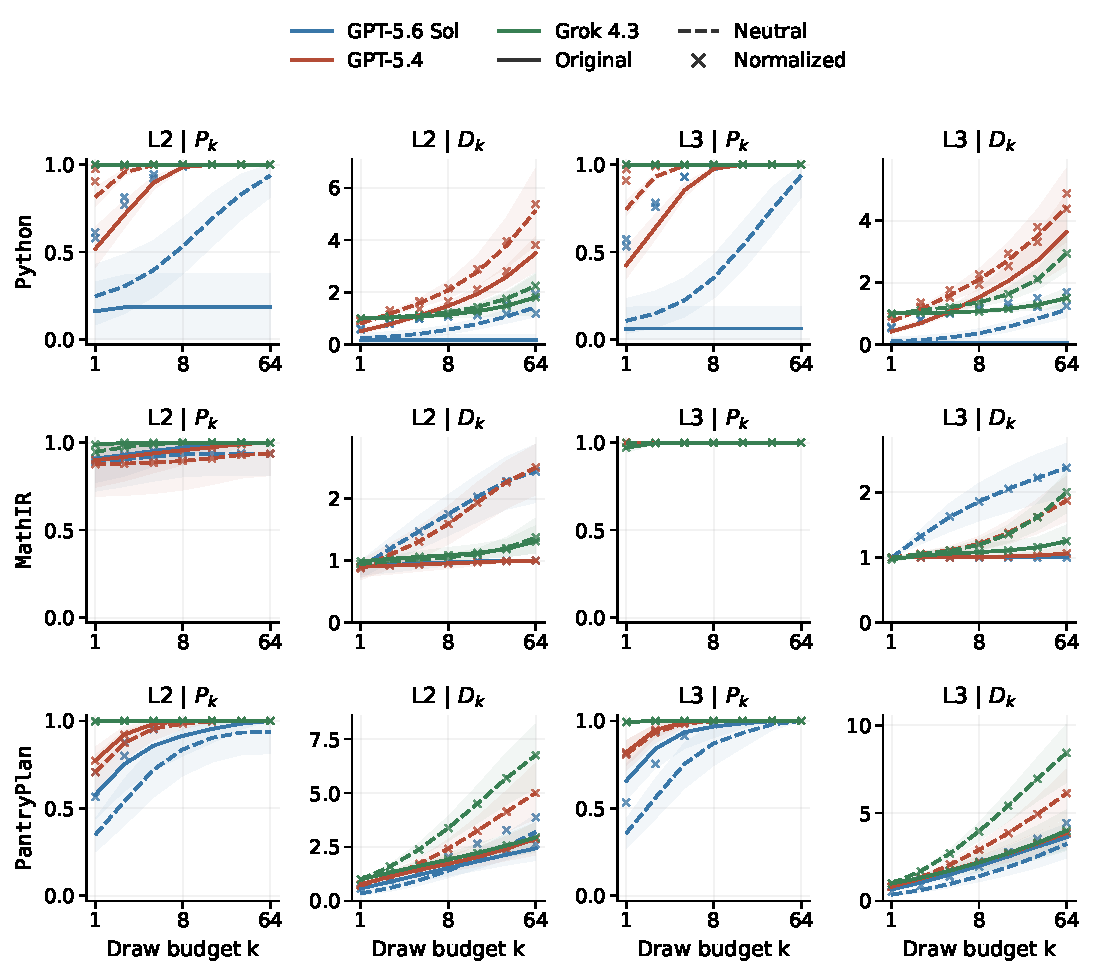
\includegraphics[width=\linewidth,height=0.72\textheight,keepaspectratio]{figures/modebench_discovery_curves_frontier.pdf}

\caption{\textbf{Additional draws reveal solution modes beyond early success.} Hosted deployments; rows show \texttt{Python}, \texttt{MathIR}, and \texttt{PantryPlan}, with paired $P_k$ and $D_k$ columns for Levels~2 and~3. Curves show pass probability $P_k$ and distinct verified modes $D_k$ against draw budget $k$, obtained by averaging over size-$k$ subsets within sixteen 64-draw problem pools per domain and level. Colours identify deployments; solid/dashed lines denote original/neutral wording. Lines use strict verification, crosses formatting normalization, and shading pointwise 95\% bootstrap intervals. Intervals resample paired problems within each domain and level and condition on the deployment.}

\label{fig:discovery-curves-frontier}

\end{figure}

\begin{table}[!htbp]
\centering\scriptsize
\setlength{\tabcolsep}{3pt}
\caption{\textbf{Pair weighting changes the summary of correct-solution diversity.} Strict 64-draw estimates for hosted deployments. Collision $C$ weights prompts by their number of correct pairs; \pmd{} weights eligible prompts equally. Absolute estimates for each wording use their own eligible prompts, whereas $\Delta\pmd$ uses only jointly eligible prompts. Thus $\Delta\pmd$ need not equal the difference between the displayed absolute estimates, and $E_O/E_N$ are separate eligibility counts. Each deployment is fixed; intervals resample paired problems.}
\label{tab:discovery-breadth-frontier}
\resizebox{\linewidth}{!}{%
\begin{tabular}{llrrrrrrrrr}
\toprule
Model & Domain/level & $C_O$ & $C_N$ & $\pmd_O$ & $\pmd_N$ & $U^{C}_O$ & $U^{\pmd}_O$ & $E_O/E_N$ & $Q_O/Q_N$ & $\Delta\pmd$ [95\%] \\
\midrule
GPT-5.4 & \texttt{Python} L2 & $0.790$ & $0.665$ & $0.257$ & $0.341$ & $0.500$ & $0.500$ & 16/16 & 10374/21720 & $+0.084\;[-0.006,+0.186]$ \\
GPT-5.6 Sol & \texttt{Python} L2 & $1.000$ & $0.974$ & $0.000$ & $0.184$ & $0.500$ & $0.500$ & 3/13 & 4467/6074 & $+0.021\;[+0.000,+0.032]$ \\
Grok 4.3 & \texttt{Python} L2 & $0.963$ & $0.938$ & $0.037$ & $0.062$ & $0.500$ & $0.500$ & 16/16 & 32256/32256 & $+0.025\;[+0.002,+0.048]$ \\
GPT-5.4 & \texttt{Python} L3 & $0.732$ & $0.620$ & $0.334$ & $0.384$ & $0.500$ & $0.500$ & 16/16 & 6747/18043 & $+0.050\;[-0.026,+0.128]$ \\
GPT-5.6 Sol & \texttt{Python} L3 & $1.000$ & $0.966$ & $0.000$ & $0.130$ & $0.500$ & $0.500$ & 1/10 & 1953/2097 & $+0.031\;[+0.031,+0.031]$ \\
Grok 4.3 & \texttt{Python} L3 & $0.981$ & $0.893$ & $0.019$ & $0.107$ & $0.500$ & $0.500$ & 16/16 & 32193/32256 & $+0.087\;[+0.041,+0.154]$ \\
GPT-5.4 & \texttt{MathIR} L2 & $1.000$ & $0.756$ & $0.000$ & $0.228$ & $0.200$ & $0.800$ & 16/15 & 28440/28227 & $+0.228\;[+0.161,+0.302]$ \\
GPT-5.6 Sol & \texttt{MathIR} L2 & $1.000$ & $0.678$ & $0.000$ & $0.302$ & $0.200$ & $0.800$ & 16/15 & 28645/28377 & $+0.302\;[+0.200,+0.402]$ \\
Grok 4.3 & \texttt{MathIR} L2 & $0.968$ & $0.985$ & $0.033$ & $0.014$ & $0.200$ & $0.800$ & 16/16 & 31600/29677 & $-0.020\;[-0.076,+0.017]$ \\
GPT-5.4 & \texttt{MathIR} L3 & $0.998$ & $0.944$ & $0.002$ & $0.056$ & $0.200$ & $0.800$ & 16/16 & 32256/32256 & $+0.054\;[+0.027,+0.087]$ \\
GPT-5.6 Sol & \texttt{MathIR} L3 & $1.000$ & $0.676$ & $0.000$ & $0.324$ & $0.200$ & $0.800$ & 16/16 & 32256/32256 & $+0.324\;[+0.208,+0.432]$ \\
Grok 4.3 & \texttt{MathIR} L3 & $0.966$ & $0.949$ & $0.033$ & $0.051$ & $0.200$ & $0.800$ & 16/16 & 30520/32193 & $+0.019\;[-0.046,+0.064]$ \\
GPT-5.4 & \texttt{PantryPlan} L2 & $0.680$ & $0.499$ & $0.252$ & $0.483$ & $0.069$ & $0.934$ & 16/16 & 20097/17436 & $+0.231\;[+0.069,+0.395]$ \\
GPT-5.6 Sol & \texttt{PantryPlan} L2 & $0.674$ & $0.624$ & $0.275$ & $0.474$ & $0.076$ & $0.934$ & 16/15 & 12941/5001 & $+0.180\;[+0.058,+0.327]$ \\
Grok 4.3 & \texttt{PantryPlan} L2 & $0.684$ & $0.412$ & $0.315$ & $0.589$ & $0.066$ & $0.934$ & 16/16 & 32005/32193 & $+0.274\;[+0.143,+0.411]$ \\
GPT-5.4 & \texttt{PantryPlan} L3 & $0.546$ & $0.392$ & $0.431$ & $0.610$ & $0.065$ & $0.937$ & 16/16 & 22332/21975 & $+0.179\;[+0.103,+0.257]$ \\
GPT-5.6 Sol & \texttt{PantryPlan} L3 & $0.566$ & $0.652$ & $0.422$ & $0.441$ & $0.061$ & $0.937$ & 16/16 & 15229/4946 & $+0.019\;[-0.136,+0.172]$ \\
Grok 4.3 & \texttt{PantryPlan} L3 & $0.673$ & $0.294$ & $0.330$ & $0.703$ & $0.063$ & $0.937$ & 16/16 & 31830/31881 & $+0.373\;[+0.224,+0.523]$ \\
\bottomrule
\end{tabular}}
\end{table}

\begin{figure}[!htbp]

\centering

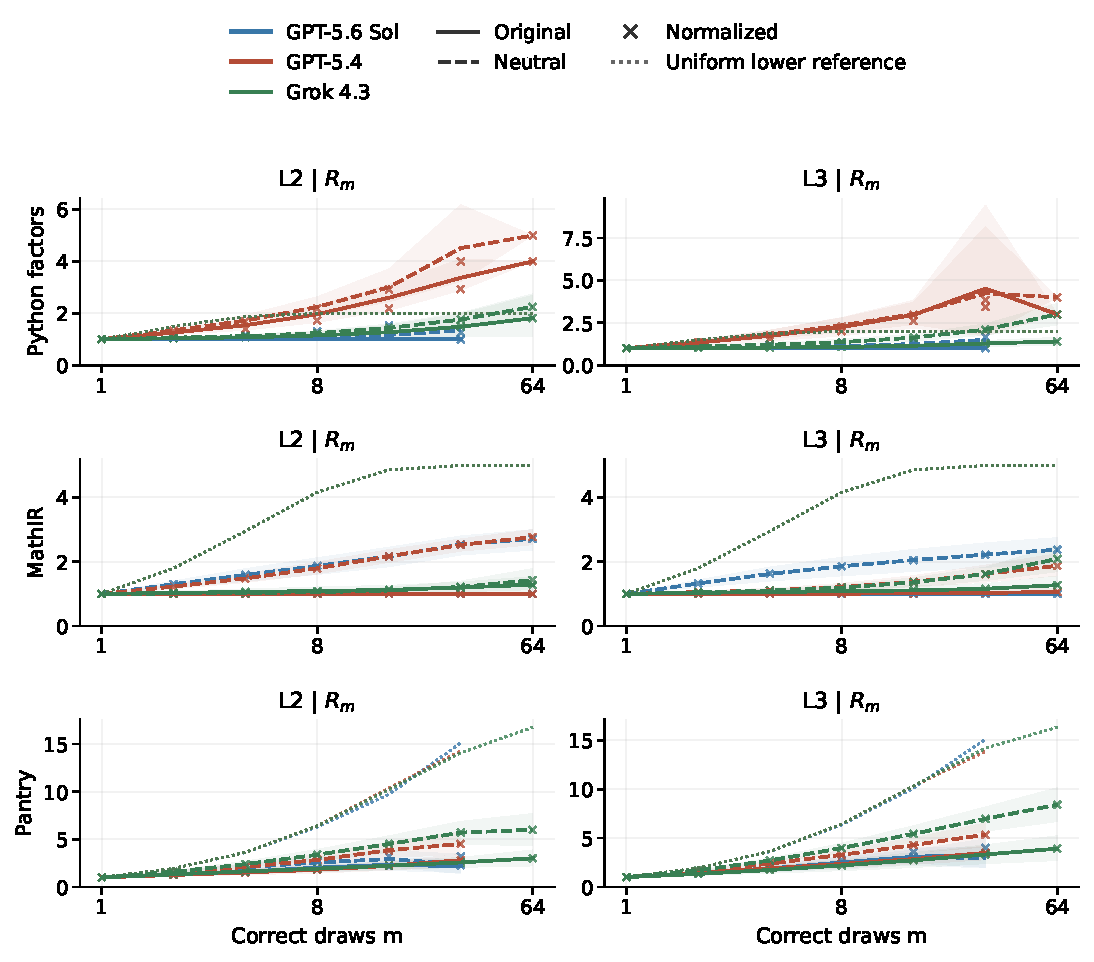
\includegraphics[width=\linewidth,height=0.66\textheight,keepaspectratio]{figures/modebench_discovery_correct_budget_frontier.pdf}

\caption{\textbf{Neutral wording broadens GPT solutions in \texttt{MathIR} at fixed correct-draw budgets.} Hosted deployments; rows show \texttt{Python}, \texttt{MathIR}, and \texttt{PantryPlan}, and columns Levels~2 and~3. Curves show $R_m$, the expected number of distinct verified modes in $m$ correct draws, on prompts with at least $m$ correct outputs under both wordings. Eligibility varies with $m$, method, and grading; gaps mark undefined means. Dotted lines give uniform lower references on prompts eligible under strict grading in both wordings, with the same prompt and checkpoint weighting as the strict curves. Colours identify deployments; solid/dashed lines denote original/neutral wording. Lines use strict verification, crosses formatting normalization, and shading pointwise 95\% bootstrap intervals. Intervals resample paired problems within each domain and level and condition on the deployment.}

\label{fig:discovery-correct-budget-frontier}

\end{figure}

\begin{table}[!htbp]
\centering\scriptsize
\setlength{\tabcolsep}{3pt}
\caption{\textbf{Discovery gains from eight to 64 draws.} Strict verification; O/N denotes original/neutral wording. Qwen2.5-0.5B-Instruct checkpoint means use five training seeds in \texttt{Python} and \texttt{MathIR} and two in \texttt{PantryPlan}; $s=1$ denotes the single initial checkpoint. Five-seed intervals resample seeds and paired prompts; \texttt{PantryPlan} intervals condition on its two checkpoints. Formatting normalization leaves every Qwen estimate unchanged.}
\label{tab:discovery-gains-local-strict}
\resizebox{\linewidth}{!}{%
\begin{tabular}{llrrrr}
\toprule
Model & Domain/level & $G_P$: O/N & $G_D$: O/N & $G_B$: O/N & $\Delta G_D$ [95\%] \\
\midrule
Dr.GRPO ($s=5$) & \texttt{Python} L2 & $0.000/0.000$ & $0.000/0.000$ & $0.000/0.000$ & $+0.000\;[+0.000,+0.000]$ \\
Initial ($s=1$) & \texttt{Python} L2 & $0.147/0.105$ & $0.303/0.165$ & $0.156/0.060$ & $-0.138\;[-0.217,-0.061]$ \\
Re:Dr ($s=5$) & \texttt{Python} L2 & $0.000/0.231$ & $0.058/0.463$ & $0.058/0.232$ & $+0.405\;[+0.185,+0.620]$ \\
Dr.GRPO ($s=5$) & \texttt{Python} L3 & $0.000/0.033$ & $0.000/0.033$ & $0.000/0.000$ & $+0.033\;[+0.000,+0.120]$ \\
Initial ($s=1$) & \texttt{Python} L3 & $0.218/0.096$ & $0.593/0.096$ & $0.376/0.000$ & $-0.497\;[-0.766,-0.270]$ \\
Re:Dr ($s=5$) & \texttt{Python} L3 & $0.000/0.239$ & $0.153/0.531$ & $0.153/0.292$ & $+0.379\;[+0.111,+0.678]$ \\
Dr.GRPO ($s=5$) & \texttt{MathIR} L2 & $0.021/0.017$ & $0.021/0.017$ & $0.000/0.000$ & $-0.004\;[-0.068,+0.045]$ \\
Initial ($s=1$) & \texttt{MathIR} L2 & $0.344/0.235$ & $0.344/0.235$ & $0.000/0.000$ & $-0.109\;[-0.383,+0.164]$ \\
Re:Dr ($s=5$) & \texttt{MathIR} L2 & $0.010/0.011$ & $0.010/0.011$ & $0.000/0.000$ & $+0.001\;[-0.036,+0.050]$ \\
Dr.GRPO ($s=5$) & \texttt{MathIR} L3 & $0.023/0.018$ & $0.026/0.018$ & $0.004/0.000$ & $-0.008\;[-0.065,+0.038]$ \\
Initial ($s=1$) & \texttt{MathIR} L3 & $0.254/0.246$ & $0.359/0.360$ & $0.105/0.114$ & $+0.001\;[-0.123,+0.095]$ \\
Re:Dr ($s=5$) & \texttt{MathIR} L3 & $0.064/0.056$ & $0.064/0.056$ & $0.000/0.000$ & $-0.008\;[-0.099,+0.059]$ \\
Dr.GRPO ($s=2$) & \texttt{PantryPlan} L2 & $0.332/0.323$ & $0.718/0.736$ & $0.386/0.414$ & $+0.018\;[-0.422,+0.433]$ \\
Initial ($s=1$) & \texttt{PantryPlan} L2 & $0.440/0.419$ & $0.857/0.955$ & $0.416/0.537$ & $+0.099\;[-0.201,+0.392]$ \\
Re:Dr ($s=2$) & \texttt{PantryPlan} L2 & $0.141/0.147$ & $0.415/0.429$ & $0.274/0.282$ & $+0.014\;[-0.123,+0.152]$ \\
Dr.GRPO ($s=2$) & \texttt{PantryPlan} L3 & $0.268/0.258$ & $0.949/1.025$ & $0.681/0.766$ & $+0.076\;[-0.237,+0.465]$ \\
Initial ($s=1$) & \texttt{PantryPlan} L3 & $0.259/0.384$ & $0.927/1.078$ & $0.668/0.694$ & $+0.151\;[-0.109,+0.399]$ \\
Re:Dr ($s=2$) & \texttt{PantryPlan} L3 & $0.204/0.149$ & $0.568/0.461$ & $0.364/0.312$ & $-0.107\;[-0.321,+0.098]$ \\
\bottomrule
\end{tabular}}
\end{table}

\begin{figure}[!htbp]

\centering

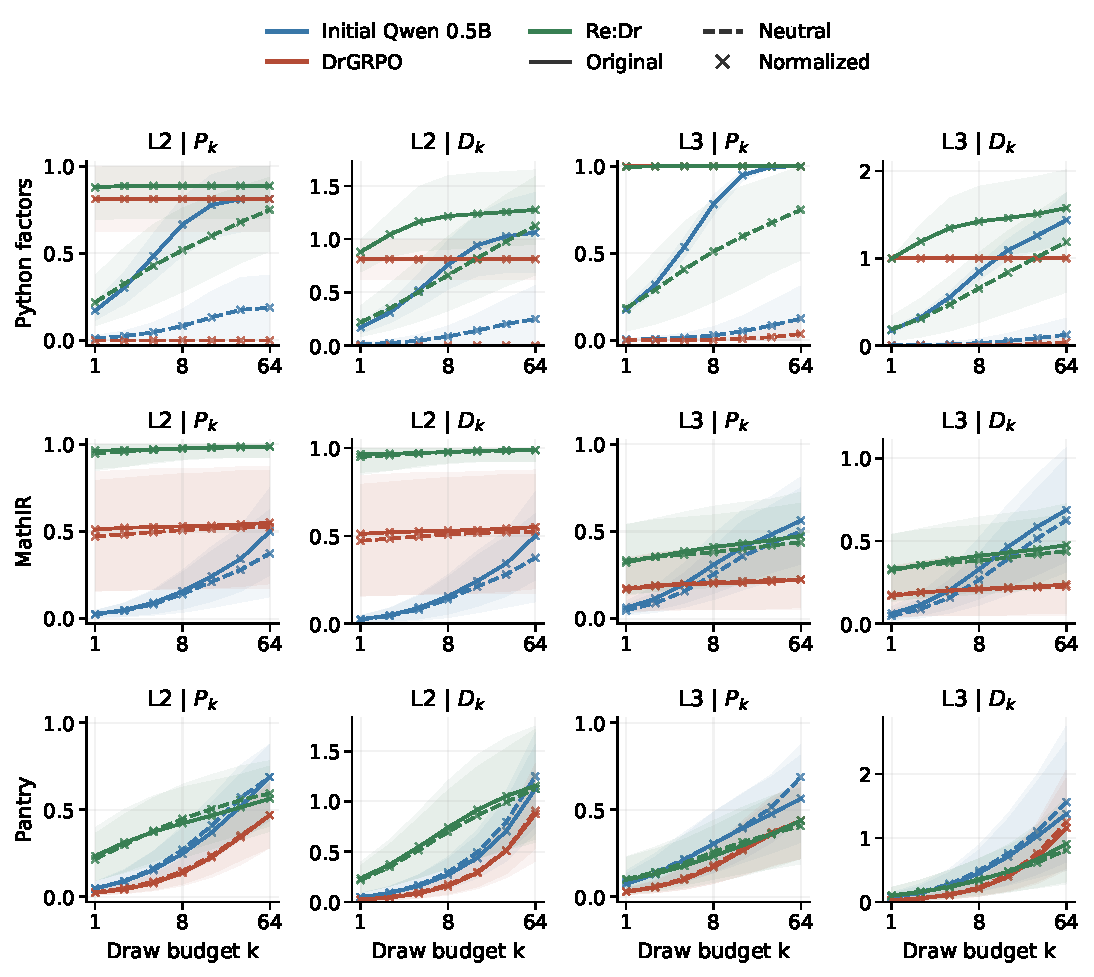
\includegraphics[width=\linewidth,height=0.72\textheight,keepaspectratio]{figures/modebench_discovery_curves_local.pdf}

\caption{\textbf{Additional draws reveal few new \texttt{MathIR} modes after training.} Qwen2.5-0.5B-Instruct checkpoints; rows show \texttt{Python}, \texttt{MathIR}, and \texttt{PantryPlan}, with paired $P_k$ and $D_k$ columns for Levels~2 and~3. Curves show pass probability $P_k$ and distinct verified modes $D_k$ against draw budget $k$, obtained by averaging over size-$k$ subsets within sixteen 64-draw problem pools per domain and level. Colours identify methods; solid/dashed lines denote original/neutral wording. Lines use strict verification, crosses formatting normalization, and shading pointwise 95\% bootstrap intervals. Means weight checkpoints equally: five training seeds in \texttt{Python} and \texttt{MathIR}, two in \texttt{PantryPlan}, and one initial checkpoint. Five-seed intervals resample seeds and paired problems; \texttt{PantryPlan} and initial intervals condition on the observed checkpoints for each method.}

\label{fig:discovery-curves-local}

\end{figure}

\begin{table}[!htbp]
\centering\scriptsize
\setlength{\tabcolsep}{3pt}
\caption{\textbf{Pair weighting changes the summary of correct-solution diversity.} Strict 64-draw estimates for Qwen2.5-0.5B-Instruct checkpoints. Collision $C$ weights prompts by their number of correct pairs; \pmd{} weights eligible prompts equally. Absolute estimates for each wording use their own eligible prompts, whereas $\Delta\pmd$ uses only jointly eligible prompts. Thus $\Delta\pmd$ need not equal the difference between the displayed absolute estimates, and $E_O/E_N$ are separate eligibility counts. Means weight checkpoints equally and are undefined if any seed lacks eligible prompts.}
\label{tab:discovery-breadth-local}
\resizebox{\linewidth}{!}{%
\begin{tabular}{llrrrrrrrrr}
\toprule
Model & Domain/level & $C_O$ & $C_N$ & $\pmd_O$ & $\pmd_N$ & $U^{C}_O$ & $U^{\pmd}_O$ & $E_O/E_N$ & $Q_O/Q_N$ & $\Delta\pmd$ [95\%] \\
\midrule
Dr.GRPO & \texttt{Python} L2 & $1.000$ & $--$ & $0.000$ & $--$ & $0.500$ & $0.500$ & 65/0 & 130977/0 & $--$ \\
Initial & \texttt{Python} L2 & $0.791$ & $0.875$ & $0.097$ & $0.167$ & $0.500$ & $0.500$ & 13/3 & 1270/24 & $-0.252\;[-0.395,+0.019]$ \\
Re:Dr & \texttt{Python} L2 & $0.809$ & $0.800$ & $0.191$ & $0.156$ & $0.500$ & $0.500$ & 71/53 & 140722/18289 & $-0.037\;[-0.139,+0.037]$ \\
Dr.GRPO & \texttt{Python} L3 & $1.000$ & $--$ & $0.000$ & $--$ & $0.500$ & $0.500$ & 80/0 & 161280/0 & $--$ \\
Initial & \texttt{Python} L3 & $0.875$ & $1.000$ & $0.101$ & $0.000$ & $0.500$ & $0.500$ & 16/1 & 1010/3 & $-0.513\;[-0.513,-0.513]$ \\
Re:Dr & \texttt{Python} L3 & $0.805$ & $0.797$ & $0.195$ & $0.227$ & $0.500$ & $0.500$ & 80/52 & 160275/12893 & $+0.030\;[-0.023,+0.117]$ \\
Dr.GRPO & \texttt{MathIR} L2 & $1.000$ & $1.000$ & $0.000$ & $0.000$ & $0.200$ & $0.800$ & 43/42 & 80766/74119 & $+0.000\;[+0.000,+0.000]$ \\
Initial & \texttt{MathIR} L2 & $1.000$ & $1.000$ & $0.000$ & $0.000$ & $0.200$ & $0.800$ & 3/3 & 64/64 & $+0.000\;[+0.000,+0.000]$ \\
Re:Dr & \texttt{MathIR} L2 & $1.000$ & $1.000$ & $0.000$ & $0.000$ & $0.200$ & $0.800$ & 79/79 & 155016/151485 & $+0.000\;[+0.000,+0.000]$ \\
Dr.GRPO & \texttt{MathIR} L3 & $0.980$ & $1.000$ & $0.038$ & $0.000$ & $0.200$ & $0.800$ & 16/18 & 24457/25393 & $-0.038\;[-0.202,+0.000]$ \\
Initial & \texttt{MathIR} L3 & $0.883$ & $0.912$ & $0.128$ & $0.162$ & $0.200$ & $0.800$ & 7/6 & 282/181 & $+0.013\;[-0.014,+0.052]$ \\
Re:Dr & \texttt{MathIR} L3 & $1.000$ & $1.000$ & $0.000$ & $0.000$ & $0.200$ & $0.800$ & 34/34 & 46891/50301 & $+0.000\;[+0.000,+0.000]$ \\
Dr.GRPO & \texttt{PantryPlan} L2 & $0.374$ & $0.276$ & $0.733$ & $0.780$ & $0.047$ & $0.953$ & 9/10 & 101/193 & $+0.220\;[-0.030,+0.470]$ \\
Initial & \texttt{PantryPlan} L2 & $0.849$ & $0.787$ & $0.587$ & $0.623$ & $0.052$ & $0.945$ & 7/10 & 212/178 & $-0.078\;[-0.300,+0.064]$ \\
Re:Dr & \texttt{PantryPlan} L2 & $0.600$ & $0.613$ & $0.343$ & $0.218$ & $0.051$ & $0.942$ & 16/18 & 10144/8510 & $-0.093\;[-0.220,+0.007]$ \\
Dr.GRPO & \texttt{PantryPlan} L3 & $0.203$ & $0.228$ & $0.808$ & $0.680$ & $0.047$ & $0.950$ & 10/12 & 134/165 & $-0.156\;[-0.359,+0.081]$ \\
Initial & \texttt{PantryPlan} L3 & $0.375$ & $0.313$ & $0.307$ & $0.341$ & $0.049$ & $0.945$ & 7/6 & 531/705 & $-0.017\;[-0.109,+0.091]$ \\
Re:Dr & \texttt{PantryPlan} L3 & $0.636$ & $0.666$ & $0.337$ & $0.198$ & $0.051$ & $0.941$ & 10/11 & 4006/3946 & $-0.112\;[-0.319,+0.008]$ \\
\bottomrule
\end{tabular}}
\end{table}

\begin{figure}[!htbp]

\centering

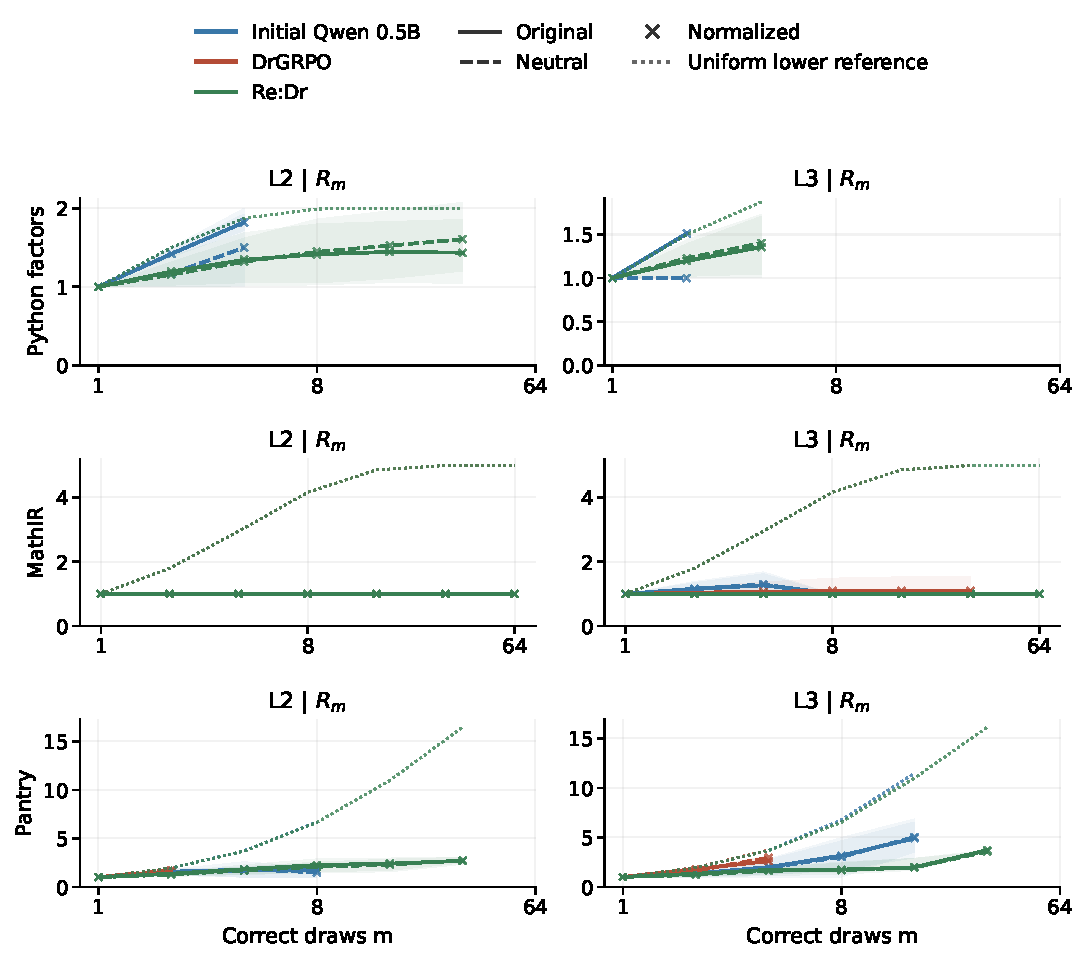
\includegraphics[width=\linewidth,height=0.66\textheight,keepaspectratio]{figures/modebench_discovery_correct_budget_local.pdf}

\caption{\textbf{\texttt{MathIR} correct solutions remain concentrated after training.} Qwen2.5-0.5B-Instruct checkpoints; rows show \texttt{Python}, \texttt{MathIR}, and \texttt{PantryPlan}, and columns Levels~2 and~3. Curves show $R_m$, the expected number of distinct verified modes in $m$ correct draws, on prompts with at least $m$ correct outputs under both wordings. Eligibility varies with $m$, method, and grading; gaps mark undefined means. Dotted lines give uniform lower references on prompts eligible under strict grading in both wordings, with the same prompt and checkpoint weighting as the strict curves. Colours identify methods; solid/dashed lines denote original/neutral wording. Lines use strict verification, crosses formatting normalization, and shading pointwise 95\% bootstrap intervals. Means weight checkpoints equally: five training seeds in \texttt{Python} and \texttt{MathIR}, two in \texttt{PantryPlan}, and one initial checkpoint. Five-seed intervals resample seeds and paired problems; \texttt{PantryPlan} and initial intervals condition on the observed checkpoints for each method.}

\label{fig:discovery-correct-budget-local}

\end{figure}


\subsection{Hosted-model discovery: wording, formatting, and additional draws}
\label{app:hosted-discovery-complete}

The hosted evaluation contains 36,864 responses from GPT-5.4, GPT-5.6 Sol,
and Grok 4.3. Each deployment receives sixteen problems from each of
\texttt{Python}, \texttt{MathIR}, and \texttt{PantryPlan} at Levels~2 and~3,
with two wordings and 64 draws per wording. All three deployments use
medium reasoning effort and an 8,192-token output cap. These settings
differ from the reasoning-disabled main-table evaluation. The \texttt{Python}
comparisons use the same mathematical problems under both wordings.
The hosted models receive no task-specific training in this evaluation.

\paragraph{Neutral wording broadens the GPT models' correct \texttt{MathIR} solutions.}
Both GPT deployments yield at most one verified mode per Level-2 problem
in 64 original-wording draws. Among problems with
at least eight correct responses under both wordings, neutral wording
increases mean breadth at eight correct draws by $.794$ ($[.623,.990]$)
for GPT-5.4 and $.872$ ($[.606,1.123]$) for GPT-5.6 Sol.
The Level-3 effects are $.204$ ($[.106,.320]$) and $.860$
($[.563,1.141]$). These comparisons include fourteen and fifteen jointly
eligible problems at Level~2, respectively, and sixteen for each GPT
deployment at Level~3. Grok 4.3's corresponding intervals include zero at
both levels.

The pointwise intervals resample the sixteen paired problems
within each domain and level, conditioning on the deployment. They do not
include variation across model training seeds. These breadth contrasts
describe jointly eligible problems without equating the wordings' accuracy.

\paragraph{Additional draws reveal more \texttt{PantryPlan} modes after first success.}
Under neutral wording, GPT-5.4 gains $2.583$ and $3.219$ verified modes
between eight and 64 draws at Levels~2 and~3; Grok 4.3 gains $3.377$ and
$4.466$. Grok 4.3's empirical pass probability is already $1.0$ at eight draws
at both levels, so these gains consist entirely of additional modes.
At Level~3 its distinct count rises from $3.972$ to $8.438$.
On jointly eligible problems at eight correct draws, neutral minus
original breadth is $1.781$ ($[1.226,2.338]$) for Grok 4.3 and $.934$
($[.670,1.184]$) for GPT-5.4; GPT-5.6 Sol's Level-3 contrast is
inconclusive. These counts measure finite-sample discovery rather than
exhaustive solution coverage.

\paragraph{Formatting limits GPT-5.6 Sol's strict \texttt{Python} scores.}
GPT-5.6 Sol's original-wording strict pass probability is approximately
$.1875$ at Level~2 and $.0625$ at Level~3 from eight through 64 draws.
Formatting normalization gives $P_{64}=1.0$ under both wordings at both
levels, with all four $P_8$ values above $.989$. The low strict scores
therefore include failures to express valid solutions in the required
format.

After normalization, the neutral-minus-original difference in
discovery gains from eight to 64 draws is $.681$ ($[.351,1.066]$) at Level~2 and $.370$
($[.112,.674]$) at Level~3. Normalization changes response formatting
before applying the same verifier and canonical-key extraction rules.


% Generated by ops/build_paper_gpt56_all_levels32_discovery.py; do not edit.
\subsection{All five domains and all three levels at 512 draws}
\label{app:gpt56-all-levels-discovery}

We evaluate GPT-5.6 Sol on thirty-two problems from each of five domains
at Levels~1, 2, and~3, using the original prompt wording. Problems are
selected independently of model outputs.
Each problem receives 512 responses: 480 problems and 245,760
responses in total. Requests use medium reasoning, an 8,192-token output
limit, and unspecified temperature and top-$p$, with model snapshot
\texttt{gpt-5.6-sol-2026-07-09}. Invalid, refused, and truncated answers remain in the sampling denominator.

Figure~\ref{fig:gpt56-sampling-budget} uses formatting-normalized grading;
Table~\ref{tab:gpt56-all-levels-endpoints} also gives strict-verifier results
on the same response pools. In draw-index order, the first 64 responses
solve 474 of 480 problems after normalization and 418 under strict grading.
At 512 responses, these counts are 477 and 436, respectively.

For a pool of $N=512$ responses, with $c$ correct responses and verified-mode counts $n_j$,
success probability and expected distinct modes in a uniformly sampled $k$-subset are
\[
 P_N(k)=1-\frac{\binom{N-c}{k}}{\binom Nk},\qquad
 D_N(k)=\sum_j\left[1-\frac{\binom{N-n_j}{k}}{\binom Nk}\right],
\]
respectively. We average all thirty-two problems equally within each
domain and level, including problems with no correct response.
Every curve uses the complete 512-response pools at budgets
$k\in\{1,2,4,8,16,32,64,128,256,512\}$. The rarefied estimate at $k=64$
need not equal the result from the first 64 responses in draw-index order.
The gain from the final budget doubling is $D_{512}(512)-D_{512}(256)$.
Pointwise 95\% intervals use 20,000 whole-problem bootstrap replicates
within domain and level; the same resampled problems
form both sides of each contrast. Intervals do not provide simultaneous
coverage across budgets, domains, or levels.

\begin{table}[!htbp]
  \centering
  \footnotesize
  \setlength{\tabcolsep}{4pt}
  \resizebox{\linewidth}{!}{%
  \begin{tabular}{llrrrrr}
    \toprule
    & & & \multicolumn{2}{c}{$D/P$ at 512} & \multicolumn{2}{c}{$\Delta D$, 256 to 512 [95\% CI]} \\
    \cmidrule(lr){4-5}\cmidrule(l){6-7}
    Domain & Level & Known support (range) & Normalized & Strict & Normalized & Strict \\
    \midrule
    \texttt{Graph} & 1 & $6.97$ (4--12) & 2.531/100.0 & 2.531/100.0 & 0.222 [0.142, 0.305] & 0.222 [0.142, 0.305] \\
    \texttt{Graph} & 2 & $6.03$ (4--12) & 2.625/100.0 & 2.625/100.0 & 0.268 [0.170, 0.373] & 0.268 [0.170, 0.373] \\
    \texttt{Graph} & 3 & $6.66$ (4--12) & 1.719/100.0 & 1.719/100.0 & 0.137 [0.059, 0.228] & 0.137 [0.059, 0.228] \\
    \addlinespace[2pt]
    \texttt{Countdown} & 1 & $\geq 4.53$ (2--6) & 3.469/100.0 & 3.375/100.0 & 0.148 [0.070, 0.243] & 0.164 [0.083, 0.259] \\
    \texttt{Countdown} & 2 & $\geq 4.40$ (3--7) & 3.156/100.0 & 3.094/100.0 & 0.218 [0.123, 0.320] & 0.235 [0.136, 0.344] \\
    \texttt{Countdown} & 3 & $\geq 4.25$ (2--8) & 2.812/100.0 & 2.562/100.0 & 0.181 [0.090, 0.289] & 0.191 [0.097, 0.297] \\
    \addlinespace[2pt]
    \texttt{Python} & 1 & $\geq 2.00$ (2) & 3.750/100.0 & 2.875/100.0 & 0.592 [0.438, 0.750] & 0.492 [0.334, 0.656] \\
    \texttt{Python} & 2 & $\geq 2.00$ (2) & 1.438/100.0 & 0.562/43.8 & 0.073 [0.020, 0.135] & 0.148 [0.078, 0.227] \\
    \texttt{Python} & 3 & $\geq 2.00$ (2) & 1.344/100.0 & 0.281/28.1 & 0.013 [0.000, 0.032] & 0.086 [0.031, 0.156] \\
    \addlinespace[2pt]
    \texttt{MathIR} & 1 & $\geq 5.00$ (5) & 1.906/93.8 & 1.906/93.8 & 0.071 [0.012, 0.153] & 0.071 [0.012, 0.153] \\
    \texttt{MathIR} & 2 & $\geq 5.00$ (5) & 1.000/100.0 & 1.000/100.0 & 0.002 [0.000, 0.006] & 0.002 [0.000, 0.006] \\
    \texttt{MathIR} & 3 & $\geq 5.00$ (5) & 0.969/96.9 & 0.969/96.9 & 0.000 [0.000, 0.000] & 0.000 [0.000, 0.000] \\
    \addlinespace[2pt]
    \texttt{PantryPlan} & 1 & $\geq 16.90$ (8--39) & 6.906/100.0 & 6.906/100.0 & 0.622 [0.458, 0.799] & 0.622 [0.458, 0.799] \\
    \texttt{PantryPlan} & 2 & $\geq 16.50$ (8--39) & 4.875/100.0 & 4.625/100.0 & 0.702 [0.476, 0.951] & 0.702 [0.472, 0.962] \\
    \texttt{PantryPlan} & 3 & $\geq 16.87$ (8--40) & 5.562/100.0 & 5.250/100.0 & 0.719 [0.527, 0.914] & 0.678 [0.489, 0.875] \\
    \bottomrule
  \end{tabular}
  }
  \caption{\textbf{Late mode discovery is largest in \texttt{PantryPlan} and Level-1 \texttt{Python}.}
  GPT-5.6 Sol with original wording and 512 responses for each of thirty-two
  problems per domain and level. $D/P$ gives mean distinct verified modes
  and the percentage of problems solved at least once.
  Support gives the mean and range within each domain and level: exact for \texttt{Graph} and a certified
  lower bound elsewhere. Strict and normalized grading use identical pools.
  The paired contrast $\Delta D=D_{512}(512)-D_{512}(256)$ measures the gain
  in expected distinct modes between random subsets of the complete pool, rather than between successive draws.
  Brackets give pointwise 95\% whole-problem bootstrap intervals.}
  \label{tab:gpt56-all-levels-endpoints}
\end{table}

The \texttt{Graph} support count includes every assignment compatible with the fixed colors.
\texttt{Countdown} references enumerate binary expression trees; the validator
also accepts unary negation and retains it in canonical keys, so these
counts are lower bounds. The \texttt{Python}, \texttt{MathIR}, and \texttt{PantryPlan} references
are also certified lower bounds. Exceeding a lower bound does not imply
that all available modes have been discovered.

Figure~\ref{fig:gpt56-sampling-budget} divides the mean distinct-mode count
by the mean enumerated mode count for the same thirty-two problems.
This ratio of means differs from the mean fraction of modes recovered per
problem; the denominator is held fixed when scaling interval endpoints.
The independently certified references in Table~\ref{tab:gpt56-all-levels-endpoints}
can be smaller than these enumerated counts. In \texttt{Python}, the table certifies
at least two modes per problem, while the mean enumerated counts used
in the figure are 222, 335.75, and 354.75 at Levels~1, 2, and~3.

These curves describe random subsets of the observed response pools.
Using them to predict discovery from new responses at each budget also
requires stable sampling behavior across requests; a common model snapshot
and decoding settings do not ensure this. Small or zero gains at the
largest budgets do not rule out rare unseen modes.


\subsection{Discovery at larger sampling budgets}
\label{app:sampling-budget-effects}

The 64-draw comparison in App.~\ref{app:sampling-budget-ablation} uses
36,864 responses from hosted models and 110,592 from Qwen checkpoints,
147,456 in total. Each of the six hosted model--wording combinations
contributes 6,144 responses. The Qwen evaluation includes 25 checkpoints:
each trained checkpoint is evaluated in its training domain at Levels~2
and~3, and the initial checkpoint covers all six domain--level combinations.
Every response remains in its sampling denominator. Formatting normalization
adds no verified Qwen responses, so both grading rules yield identical
estimates for these checkpoints. The sixteen problems per domain and level
differ from the thirty-two used in the 512-draw study
(App.~\ref{app:gpt56-all-levels-discovery}).

\paragraph{Prompt weighting changes the diversity summary.}
Tables~\ref{tab:discovery-breadth-frontier} and~\ref{tab:discovery-breadth-local}
compare two summaries of the 64-response pools. Within each checkpoint or
deployment, collision $C$ pools correct pairs across prompts, weighting each
prompt in proportion to $\binom{c}{2}$. Promptwise \pmd{} gives equal weight
to each prompt with at least two verified responses. Trained-checkpoint
scores then receive equal weight across seeds. Across 70 defined
combinations of model, domain, level, and wording, the median absolute
difference between promptwise \pmd{} and $1-C$ is $.003$, but nineteen
differ by at least $.05$.

For the initial checkpoint under original wording,
Level-2 \texttt{PantryPlan} has $1-C=.151$ and promptwise \pmd{} of $.587$;
Level~3 has $.625$ and $.307$, respectively. Both estimates use seven of
sixteen problems. The direction of the difference depends on which prompts
supply the most correct pairs and therefore receive the largest weights.

Neither weighting holds overall accuracy or the eligible population fixed.
For the initial checkpoint, Level-3 \texttt{Python} has sixteen eligible
problems under original wording and one under neutral wording. Each wording's
absolute estimate uses its own eligible prompts; paired differences use
only jointly eligible prompts. Equal prompt weights therefore describe
conditional diversity within these selected populations
(App.~\ref{app:metric-sampling}).

\paragraph{\texttt{MathIR}: concentration largely persists through 64 draws.}
At Level~2, both trained methods have $B_k=0$ at every measured budget under
both wordings. Re:Dr has $P_8=.9774$ and $P_{64}=.9875$ under original
wording, compared with $.9767$ and $.9875$ under neutral wording. Its $D_k$
equals $P_k$ throughout, so the small increase comes entirely from first
successes. At a budget of eight correct draws, both wordings have $R_8=1$
on the same 76 eligible checkpoint--problem pairs, compared with the
uniform lower reference $5[1-(4/5)^8]=4.1611$ from certified support.
These pairs reuse the same 16 problems across five checkpoints.

At Level~3, both trained methods under neutral wording and Re:Dr under
original wording also yield at most one correct key per checkpoint and
problem. Dr.GRPO under original wording has one exception: one checkpoint--problem
pair contains two keys with counts 28 and 9. Averaging over seeds and problems
gives $B_{64}=.0125$ and $B_{64}-B_8=.0035$. The corresponding equal-seed
correct-pair collision is $.9803$; the other trained \texttt{MathIR}
conditions have collision $1.0$, against the uniform upper reference $.2$.
The larger budget thus reveals a rare additional mode, precluding an exact
single-mode description of every trained condition.

\paragraph{\texttt{Python}: prompt dependence and additional discovery coexist.}
Under original wording, Dr.GRPO has $P_k=D_k=.8125$ at Level~2 and $1.0$
at Level~3 throughout the range from eight to 64 draws. Under neutral wording,
it has zero correct responses out of 5,120 at Level~2 and three out of
5,120 at Level~3. Each success is the only correct response for its
checkpoint--problem pair. The Level~3 mean is therefore
$P_{64}=D_{64}=.0375$, while correct-pair collision remains undefined.

For Re:Dr under original wording, pass probability is unchanged from eight
to 64 draws, but $D_k$ increases by $.0582$ at Level~2 and $.1529$ at
Level~3. Under neutral wording, $P_k$ rises from $.5186$ to $.7500$ and
from $.5109$ to $.7500$, respectively; $D_k$ rises from $.6618$ to $1.1250$
and from $.6561$ to $1.1875$. These final mode counts remain below the
original-wording values of $1.2750$ and $1.5750$. The corresponding gains
in modes beyond the first success are $.2318$ [$.0574,.4565$] and $.2923$
[$.0659,.5445$], with intervals that resample seeds and paired problems.
Larger budgets therefore recover both first successes and additional
verified alternatives for Re:Dr under neutral wording. These unconditional
gains alone do not identify a change in the conditional distribution of
correct solutions.

\paragraph{\texttt{PantryPlan}: eight draws understate observed discovery.}
Across trained checkpoints at both levels and under both wordings,
$D_{64}-D_8$ ranges from $.4151$ to $1.0247$, with gains in modes beyond
the first success ranging from $.2739$ to $.7664$. The initial checkpoint
also gains $.8565$--$1.0778$ modes. For the two observed training seeds,
the Level~3 method ordering changes with the sampling budget. Under original
wording, Dr.GRPO/Re:Dr have $D_8=.2075/.3381$ but
$D_{64}=1.1563/.9063$; neutral wording gives $.2253/.3515$ at eight draws
and $1.2500/.8125$ at 64. These rankings describe the observed checkpoints
and do not establish a population-level method advantage.

\texttt{PantryPlan} has only two training seeds. Comparisons at larger
correct-draw budgets $m$ often have few or no jointly eligible problems.
They condition on observed success, and the equal-seed mean is undefined
when either seed has no eligible problem.

Several trained conditions remain concentrated at 64 draws, while others
continue to yield additional solution modes. A flat curve over a finite
response pool still leaves open the possibility of rare unseen modes.
Here the $k=8$ points average subsets of sixteen 64-response pools per
domain and level; App.~\ref{app:prompt-hint-ablation} uses a separate
eight-draw evaluation on thirty-two problems per domain and level.
The checkpoints are trained at Level~2, so Level~3 results measure transfer;
hosted results describe fixed deployments.


% Concise theory for both papers; full derivations are preserved in
% paper/audits/streamlining_20260911/full_theory.tex.

% Generated by ops/build_paper_inference_followups.py; do not edit numbers.
\section{Inference: Adaptation, Model Mixtures, and Coarser Keys}
\label{app:inference-followups}
We evaluate adaptation to changed requirements, complementarity between
models, and sensitivity to the definition of a solution mode. Model weights
remain fixed during inference. Pointwise 95\% percentile intervals use 20,000
paired whole-problem bootstrap replicates. Resampling preserves all
perturbations, model conditions, and training seeds for each problem;
hosted comparisons resample within each domain and level. These intervals
condition on the observed response pools and training seeds, so they do not
estimate variability across new response pools or training seeds. The 21
model-pair comparisons are dependent, and intervals are unadjusted for
multiple comparisons.

\subsection{\texttt{PantryPlan} portfolios under changed requirements}
\label{app:pantry-adaptation}
We evaluate the initial Qwen2.5-0.5B checkpoint and Level-2 Dr.GRPO and
Re:Dr checkpoints from two matched training seeds on 32 held-out problems.
We derive 192 single-ingredient outages from the task specifications,
independently of generated answers. Exhaustive search over the original
quantity grid finds valid plans for 181 revised tasks. These plans establish
feasibility and are withheld from the model. Five feasible additional dietary
restrictions are reported separately, as they cover only five source problems.

Each portfolio contains eight plans, which we test unchanged against the
revised requirements. If none remains valid, we allow up to eight sequential
recovery calls and stop at the first valid plan. Unresolved portfolios use
all eight calls. Each recovery prompt contains the revised task, initial
portfolio, previous recovery outputs, and deterministic verifier feedback.
Cumulative success includes portfolios that require no recovery. We average
over perturbations within each source problem, then weight problems equally.

The three sampling strategies use the same checkpoints, verifier, and
192-token response cap. Ordinary sampling uses temperature 1.0. Temperature
tuning selects from $\{0.7,1.0,1.3\}$ based on outage survival on 16 separate
development problems (384 responses per checkpoint). Diversity prompting
makes eight sequential calls, requesting a plan with a new ingredient support
and retaining the complete output history, including failures. All strategies
use the same number of initial responses, but their context lengths and total
token costs differ.

\begin{figure}[!htbp]
\centering
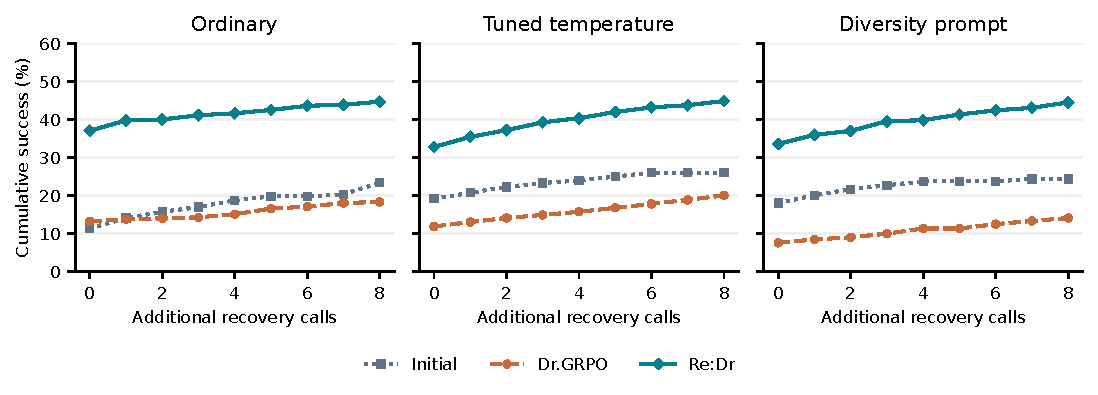
\includegraphics[width=\linewidth]{figures/pantry_adaptation_recovery_20260912.pdf}
\caption{\textbf{Re:Dr improves portfolio survival and success within eight
recovery calls.} Panels compare ordinary sampling, tuned temperature, and
diversity prompting on the same 181 feasible ingredient outages from 32
\texttt{PantryPlan} problems. The horizontal axis is the additional recovery-call budget;
the vertical axis includes success without recovery at zero calls. Curves
average outages within problems, then problems equally. Solid diamonds show
Re:Dr, dashed circles Dr.GRPO, and dotted squares the initial checkpoint;
trained curves average two matched seeds. Pointwise 95\% intervals for
paired differences appear in Table~\ref{tab:pantry-adaptation-contrasts}.}
\label{fig:pantry-adaptation-recovery}
\end{figure}

\begin{table}[!htbp]
\centering
\caption{\textbf{Re:Dr portfolios adapt better to ingredient outages across all three sampling strategies.} Eight initial plans face 181 feasible outages from 32 problems or five additional dietary restrictions from five problems. Survival is success without recovery; By 8 includes success within eight recovery calls (both percentages). Calls count unresolved cases as eight. Token totals count the initial portfolio once per revised task. Entries average perturbations within problems, then problems equally; dietary estimates use only five problems. Labels (a) and (b) denote the two matched training replicates.}
\label{tab:pantry-adaptation}
\scriptsize
\setlength{\tabcolsep}{3pt}
\begin{tabular}{lllrrrrr}
\toprule
Change & Checkpoint & Strategy & Survival & By 8 & Calls & Input tokens & Output tokens \\
\midrule
Outages & Initial & Ordinary & 11.35 & 23.44 & 6.63 & 11301.75 & 376.49 \\
 & Initial & Tuned temperature & 19.17 & 26.04 & 6.13 & 10864.88 & 370.17 \\
 & Initial & Diversity prompt & 18.02 & 24.38 & 6.22 & 11794.81 & 352.87 \\
 & Dr.GRPO (a) & Ordinary & 9.79 & 14.01 & 7.09 & 12439.22 & 823.70 \\
 & Dr.GRPO (a) & Tuned temperature & 13.44 & 16.77 & 6.79 & 12017.57 & 775.44 \\
 & Dr.GRPO (a) & Diversity prompt & 5.21 & 8.39 & 7.44 & 14103.23 & 848.09 \\
 & Dr.GRPO (b) & Ordinary & 16.67 & 22.60 & 6.47 & 11265.39 & 637.59 \\
 & Dr.GRPO (b) & Tuned temperature & 10.31 & 23.39 & 6.75 & 11531.40 & 644.94 \\
 & Dr.GRPO (b) & Diversity prompt & 9.90 & 19.79 & 6.90 & 13124.10 & 731.00 \\
 & Re:Dr (a) & Ordinary & 39.38 & 47.97 & 4.47 & 9078.92 & 297.98 \\
 & Re:Dr (a) & Tuned temperature & 28.23 & 40.94 & 5.19 & 9718.01 & 310.50 \\
 & Re:Dr (a) & Diversity prompt & 36.93 & 47.19 & 4.68 & 10465.22 & 344.02 \\
 & Re:Dr (b) & Ordinary & 34.74 & 41.51 & 4.94 & 9547.16 & 308.52 \\
 & Re:Dr (b) & Tuned temperature & 37.34 & 48.85 & 4.53 & 9148.77 & 300.05 \\
 & Re:Dr (b) & Diversity prompt & 30.26 & 41.93 & 5.06 & 10584.02 & 313.50 \\
\midrule
Dietary & Initial & Ordinary & 0.00 & 20.00 & 6.80 & 11392.80 & 371.20 \\
 & Initial & Tuned temperature & 20.00 & 40.00 & 6.40 & 11175.20 & 387.20 \\
 & Initial & Diversity prompt & 0.00 & 0.00 & 8.00 & 13630.20 & 405.00 \\
 & Dr.GRPO (a) & Ordinary & 0.00 & 0.00 & 8.00 & 13310.20 & 849.20 \\
 & Dr.GRPO (a) & Tuned temperature & 0.00 & 0.00 & 8.00 & 13394.60 & 856.00 \\
 & Dr.GRPO (a) & Diversity prompt & 0.00 & 0.00 & 8.00 & 15045.40 & 939.60 \\
 & Dr.GRPO (b) & Ordinary & 0.00 & 20.00 & 7.40 & 12063.00 & 650.40 \\
 & Dr.GRPO (b) & Tuned temperature & 0.00 & 0.00 & 8.00 & 12544.20 & 615.40 \\
 & Dr.GRPO (b) & Diversity prompt & 0.00 & 0.00 & 8.00 & 14132.40 & 725.60 \\
 & Re:Dr (a) & Ordinary & 20.00 & 60.00 & 5.20 & 9732.60 & 326.00 \\
 & Re:Dr (a) & Tuned temperature & 40.00 & 40.00 & 4.80 & 9402.80 & 307.60 \\
 & Re:Dr (a) & Diversity prompt & 40.00 & 40.00 & 4.80 & 10693.60 & 355.60 \\
 & Re:Dr (b) & Ordinary & 40.00 & 80.00 & 3.20 & 7853.20 & 271.20 \\
 & Re:Dr (b) & Tuned temperature & 40.00 & 80.00 & 3.60 & 8127.80 & 265.20 \\
 & Re:Dr (b) & Diversity prompt & 20.00 & 40.00 & 5.00 & 10738.20 & 341.00 \\
\bottomrule
\end{tabular}
\end{table}


\begin{table}[!htbp]
\centering
\caption{\textbf{Re:Dr raises outage survival and reduces recovery calls.} Entries are Re:Dr minus Dr.GRPO, averaged over two matched seeds on 32 paired problems. Survival and success by eight calls are percentage-point differences; calls include unresolved cases. Brackets are pointwise 95\% paired problem-bootstrap intervals, conditional on the observed training seeds.}
\label{tab:pantry-adaptation-contrasts}
\scriptsize
\setlength{\tabcolsep}{3pt}
\begin{tabular}{lrrr}
\toprule
Strategy & $\Delta$ survival & $\Delta$ by 8 calls & $\Delta$ calls \\
\midrule
Ordinary & $23.83$ $[12.16, 35.89]$ & $26.43$ $[14.69, 38.18]$ & $-2.08$ $[-3.03, -1.14]$ \\
Tuned temperature & $20.91$ $[9.19, 32.89]$ & $24.82$ $[14.04, 35.52]$ & $-1.91$ $[-2.78, -1.05]$ \\
Diversity prompt & $26.04$ $[16.93, 35.65]$ & $30.47$ $[21.51, 39.27]$ & $-2.30$ $[-3.04, -1.57]$ \\
\bottomrule
\end{tabular}
\end{table}

With ordinary sampling, Re:Dr improves survival over Dr.GRPO by 23.83 percentage points
$[12.16,35.89]$, reduces the mean number of recovery calls, capped at eight, by 2.08
$[1.14,3.03]$, and improves success within eight recovery calls by 26.43 points
$[14.69,38.18]$. Mean input and output token totals fall by 2,539.27
$[1,618.01,3,468.86]$ and 427.40 $[386.83,466.30]$, respectively.
The initial portfolios also contain 1.234 more correct responses out of
eight $[.578,1.984]$. Restricting each paired-seed comparison to portfolios
with equal observed correct counts leaves a 1.05-percentage-point survival
gain $[0.00,3.53]$. We first average eligible seed comparisons within each
problem, then average the 19 problems with at least one eligible comparison.
This restriction changes both the problem and seed composition, and equal
observed counts do not establish equal underlying accuracy. The adaptation
gains therefore do not isolate diversity as their causal mechanism.

Per-perturbation token totals represent deploying one portfolio and recovering
from one change in requirements. Input counts include reused prefixes and
do not measure the compute saved by prefix caching. Table~\ref{tab:pantry-collection-cost}
counts each response once across temperature selection, initial portfolios
from tuned-temperature sampling and diversity prompting, and recovery under
all three strategies. It excludes ordinary initial-portfolio generation.
Neither inference cost summary includes training costs.

\begin{table}[!htbp]
\centering
\caption{\textbf{Inference costs include temperature selection and recovery.} Each checkpoint selects $T$ from 384 responses on 16 development problems. Inference totals include this calibration, initial portfolios for tuned-temperature and diversity prompting, and recovery under all three strategies on 32 evaluation problems. Ordinary initial-portfolio generation is excluded. Each response is counted once, including reused input prefixes. Seconds report generation time, excluding training, without hardware normalization. Labels (a) and (b) denote matched training replicates.}
\label{tab:pantry-collection-cost}
\scriptsize
\setlength{\tabcolsep}{3pt}
\begin{tabular}{llrrrrr}
\toprule
Checkpoint & Scope & $T$ & Responses & Input tokens & Output tokens & Seconds \\
\midrule
Dr.GRPO (a) & Calibration & 1.3 & 384 & 229392 & 19871 & 136.3 \\
Dr.GRPO (a) & Inference total & 1.3 & 4874 & 4870884 & 272484 & 3302.0 \\
Dr.GRPO (b) & Calibration & 1.3 & 384 & 229392 & 15544 & 126.5 \\
Dr.GRPO (b) & Inference total & 1.3 & 4634 & 4365524 & 220458 & 2792.9 \\
Re:Dr (a) & Calibration & 0.7 & 384 & 229392 & 8552 & 111.1 \\
Re:Dr (a) & Inference total & 0.7 & 3559 & 3160284 & 92227 & 1527.7 \\
Re:Dr (b) & Calibration & 1.0 & 384 & 229392 & 8585 & 112.5 \\
Re:Dr (b) & Inference total & 1.0 & 3592 & 3169337 & 88300 & 1510.2 \\
Initial & Calibration & 1.3 & 384 & 229392 & 9521 & 123.5 \\
Initial & Inference total & 1.3 & 4416 & 4035069 & 116619 & 1957.4 \\
\bottomrule
\end{tabular}
\end{table}


\subsection{Complementarity across hosted models}
\label{app:cross-model-overlap}
Seven hosted models each produce eight responses to the same 1,920 prompts
(five domains, three levels, and 128 prompts per domain and level), totaling
107,520 responses. We use strict grading and the original Opus 5 \texttt{Python}
interface; the formatting-normalized hosted comparison uses a revised
Opus 5 interface. For each of the 21 model pairs, a mixed portfolio draws four
responses without replacement from each model's eight-response pool. We
compute its expected distinct-mode count exactly over all $\binom{8}{4}^2=4{,}900$
subset pairs, then compare with each constituent's complete eight-response
portfolio and their average. These are expectations within the finite
response pools, conditional on the outputs generated.

Every mixture increases the expected number of distinct solution modes
relative to its average constituent by $.115$--$.266$. Ten pairs improve
on both constituents in point estimates; nine have pointwise intervals
entirely above zero against both. On
prompts with at least four correct responses from each model, we also compare
a mixture of two correct draws per model with four correct draws from either
constituent. All pairwise gains over the average constituent remain positive
($.073$--$.177$ modes). Fixing the number of correct draws conditions on a
different eligible subset for each pair. It does not equate accuracy or the
number of attempts required to obtain those correct responses.

\begin{table}[!htbp]
\centering
\caption{\textbf{Every model pair increases expected distinct modes over its average constituent.} A 4+4 mixture samples without replacement from the two eight-response pools; A and B name the constituents in order. Panel A compares with their average: fine and coarse keys use all 1,920 prompts, while the four-correct-draw comparison uses $n$ prompts with at least four correct responses per model (2+2 mixed versus four per constituent). Panel B compares fine-key distinct modes with each constituent and pass@8 with their average. Entries are distinct-mode differences except pass@8, in percentage points. Brackets are pointwise 95\% paired problem-bootstrap intervals, stratified by domain and level; comparisons share models and prompts.}
\label{tab:cross-model-mixtures}
\scriptsize
\setlength{\tabcolsep}{3pt}
\textbf{A}\par\smallskip
\resizebox{\linewidth}{!}{%
\begin{tabular}{lrrrr}
\toprule
Pair & Fine & Coarse & Four correct draws & $n$ \\
\midrule
DeepSeek V4 Pro + Kimi K3 & $0.148$ $[0.136, 0.160]$ & $0.142$ $[0.131, 0.154]$ & $0.107$ $[0.098, 0.115]$ & 1858 \\
DeepSeek V4 Pro + Opus 4.8 & $0.198$ $[0.185, 0.211]$ & $0.183$ $[0.171, 0.197]$ & $0.153$ $[0.142, 0.164]$ & 1847 \\
DeepSeek V4 Pro + Opus 5 & $0.262$ $[0.249, 0.275]$ & $0.252$ $[0.240, 0.265]$ & $0.177$ $[0.165, 0.190]$ & 1510 \\
DeepSeek V4 Pro + GPT-5.4 & $0.133$ $[0.122, 0.143]$ & $0.127$ $[0.116, 0.138]$ & $0.098$ $[0.090, 0.107]$ & 1695 \\
DeepSeek V4 Pro + GPT-5.6 Sol & $0.235$ $[0.223, 0.247]$ & $0.224$ $[0.212, 0.237]$ & $0.154$ $[0.142, 0.166]$ & 1396 \\
DeepSeek V4 Pro + Grok 4.3 & $0.123$ $[0.112, 0.134]$ & $0.117$ $[0.106, 0.127]$ & $0.091$ $[0.083, 0.099]$ & 1859 \\
Kimi K3 + Opus 4.8 & $0.187$ $[0.174, 0.200]$ & $0.172$ $[0.159, 0.185]$ & $0.138$ $[0.127, 0.148]$ & 1885 \\
Kimi K3 + Opus 5 & $0.266$ $[0.253, 0.279]$ & $0.255$ $[0.242, 0.268]$ & $0.162$ $[0.150, 0.175]$ & 1543 \\
Kimi K3 + GPT-5.4 & $0.127$ $[0.115, 0.139]$ & $0.112$ $[0.101, 0.124]$ & $0.083$ $[0.075, 0.092]$ & 1720 \\
Kimi K3 + GPT-5.6 Sol & $0.202$ $[0.190, 0.214]$ & $0.195$ $[0.183, 0.207]$ & $0.093$ $[0.083, 0.104]$ & 1417 \\
Kimi K3 + Grok 4.3 & $0.115$ $[0.104, 0.126]$ & $0.110$ $[0.099, 0.121]$ & $0.073$ $[0.066, 0.080]$ & 1900 \\
Opus 4.8 + Opus 5 & $0.187$ $[0.176, 0.199]$ & $0.182$ $[0.171, 0.193]$ & $0.098$ $[0.087, 0.109]$ & 1534 \\
Opus 4.8 + GPT-5.4 & $0.201$ $[0.186, 0.215]$ & $0.185$ $[0.172, 0.199]$ & $0.156$ $[0.144, 0.168]$ & 1713 \\
Opus 4.8 + GPT-5.6 Sol & $0.247$ $[0.234, 0.261]$ & $0.237$ $[0.223, 0.250]$ & $0.151$ $[0.138, 0.164]$ & 1409 \\
Opus 4.8 + Grok 4.3 & $0.180$ $[0.167, 0.194]$ & $0.171$ $[0.158, 0.184]$ & $0.141$ $[0.130, 0.153]$ & 1894 \\
Opus 5 + GPT-5.4 & $0.228$ $[0.215, 0.241]$ & $0.217$ $[0.204, 0.230]$ & $0.158$ $[0.145, 0.171]$ & 1493 \\
Opus 5 + GPT-5.6 Sol & $0.169$ $[0.157, 0.182]$ & $0.161$ $[0.149, 0.174]$ & $0.143$ $[0.130, 0.156]$ & 1370 \\
Opus 5 + Grok 4.3 & $0.231$ $[0.219, 0.244]$ & $0.225$ $[0.213, 0.237]$ & $0.145$ $[0.133, 0.157]$ & 1547 \\
GPT-5.4 + GPT-5.6 Sol & $0.156$ $[0.145, 0.167]$ & $0.147$ $[0.136, 0.158]$ & $0.094$ $[0.084, 0.104]$ & 1400 \\
GPT-5.4 + Grok 4.3 & $0.130$ $[0.119, 0.142]$ & $0.121$ $[0.111, 0.132]$ & $0.095$ $[0.086, 0.104]$ & 1722 \\
GPT-5.6 Sol + Grok 4.3 & $0.211$ $[0.199, 0.224]$ & $0.204$ $[0.192, 0.216]$ & $0.118$ $[0.107, 0.130]$ & 1418 \\
\bottomrule
\end{tabular}
}
\par\medskip
\textbf{B}\par\smallskip
\resizebox{\linewidth}{!}{%
\begin{tabular}{lrrr}
\toprule
Pair & $\Delta D$ vs A & $\Delta D$ vs B & $\Delta$ pass@8 vs mean \\
\midrule
DeepSeek V4 Pro + Kimi K3 & $0.279$ $[0.254, 0.304]$ & $0.017$ $[-0.008, 0.043]$ & $0.22$ $[0.08, 0.39]$ \\
DeepSeek V4 Pro + Opus 4.8 & $0.089$ $[0.064, 0.114]$ & $0.307$ $[0.282, 0.332]$ & $0.31$ $[0.15, 0.49]$ \\
DeepSeek V4 Pro + Opus 5 & $-0.061$ $[-0.082, -0.039]$ & $0.585$ $[0.560, 0.610]$ & $7.48$ $[7.19, 7.78]$ \\
DeepSeek V4 Pro + GPT-5.4 & $0.097$ $[0.074, 0.121]$ & $0.168$ $[0.145, 0.192]$ & $0.64$ $[0.41, 0.90]$ \\
DeepSeek V4 Pro + GPT-5.6 Sol & $-0.003$ $[-0.025, 0.019]$ & $0.473$ $[0.447, 0.500]$ & $7.16$ $[6.71, 7.62]$ \\
DeepSeek V4 Pro + Grok 4.3 & $0.059$ $[0.037, 0.082]$ & $0.186$ $[0.163, 0.210]$ & $0.34$ $[0.17, 0.52]$ \\
Kimi K3 + Opus 4.8 & $-0.053$ $[-0.080, -0.027]$ & $0.427$ $[0.401, 0.452]$ & $0.19$ $[0.07, 0.32]$ \\
Kimi K3 + Opus 5 & $-0.188$ $[-0.212, -0.165]$ & $0.719$ $[0.692, 0.747]$ & $7.34$ $[7.08, 7.61]$ \\
Kimi K3 + GPT-5.4 & $-0.040$ $[-0.064, -0.015]$ & $0.293$ $[0.267, 0.320]$ & $0.73$ $[0.48, 1.00]$ \\
Kimi K3 + GPT-5.6 Sol & $-0.167$ $[-0.191, -0.144]$ & $0.571$ $[0.543, 0.600]$ & $7.38$ $[6.92, 7.85]$ \\
Kimi K3 + Grok 4.3 & $-0.080$ $[-0.104, -0.056]$ & $0.309$ $[0.284, 0.335]$ & $0.12$ $[0.03, 0.23]$ \\
Opus 4.8 + Opus 5 & $-0.027$ $[-0.045, -0.009]$ & $0.401$ $[0.379, 0.423]$ & $7.42$ $[7.14, 7.71]$ \\
Opus 4.8 + GPT-5.4 & $0.274$ $[0.248, 0.300]$ & $0.127$ $[0.101, 0.153]$ & $0.93$ $[0.65, 1.24]$ \\
Opus 4.8 + GPT-5.6 Sol & $0.118$ $[0.096, 0.141]$ & $0.377$ $[0.350, 0.403]$ & $7.51$ $[7.03, 7.99]$ \\
Opus 4.8 + Grok 4.3 & $0.226$ $[0.202, 0.250]$ & $0.135$ $[0.110, 0.160]$ & $0.11$ $[0.02, 0.23]$ \\
Opus 5 + GPT-5.4 & $0.515$ $[0.489, 0.541]$ & $-0.060$ $[-0.082, -0.037]$ & $6.30$ $[5.90, 6.71]$ \\
Opus 5 + GPT-5.6 Sol & $0.254$ $[0.232, 0.277]$ & $0.084$ $[0.063, 0.106]$ & $2.11$ $[1.66, 2.57]$ \\
Opus 5 + Grok 4.3 & $0.490$ $[0.467, 0.514]$ & $-0.028$ $[-0.048, -0.007]$ & $7.41$ $[7.13, 7.69]$ \\
GPT-5.4 + GPT-5.6 Sol & $-0.046$ $[-0.067, -0.025]$ & $0.359$ $[0.335, 0.383]$ & $5.61$ $[5.15, 6.08]$ \\
GPT-5.4 + Grok 4.3 & $0.102$ $[0.078, 0.127]$ & $0.159$ $[0.135, 0.182]$ & $0.93$ $[0.65, 1.23]$ \\
GPT-5.6 Sol + Grok 4.3 & $0.386$ $[0.360, 0.412]$ & $0.037$ $[0.015, 0.058]$ & $7.55$ $[7.08, 8.04]$ \\
\bottomrule
\end{tabular}
}
\end{table}

Cross-model collision ranges from $.624$ to $.740$, compared with $.704$
to $.819$ for mean within-model collision. Each pair gives equal weight
to prompts with $\geq2$ correct responses from each model. Absence of
observed overlap does not establish disjoint supports. Gains relative to
the average constituent persist with coarser keys and formatting-normalized
grading. Equal response counts do not equate token use, compute, monetary
cost, or reasoning interfaces across providers. These comparisons of finite
response pools do not identify causal training mechanisms.

\subsection{Sensitivity to task-relevant equivalences}
\label{app:coarser-keys}
We merge solution keys according to task-relevant equivalences and recompute
diversity. \texttt{Graph} merges global color renamings that fix every anchored color;
vertex identities remain fixed. \texttt{Python} groups opposite members $d$ and $n/d$ of the
same unordered proper factor pair, retaining input-vector order. \texttt{Countdown}
flattens associative additions and multiplications and sorts their children,
preserving operands, multiplicity, and subtraction/division boundaries.
\texttt{MathIR} retains its simplified state trajectory, and \texttt{PantryPlan} retains
ingredient supports, whose differences can affect survival under outages. The same domain-specific
map applies to each model's correct responses. Correctness is unchanged;
deterministic merging cannot increase the observed distinct-mode count or
reduce correct-pair collision.

Uniform mass over fine keys generally induces unequal mass across coarse
groups. For \texttt{Graph} and \texttt{Python}, exhaustive enumeration determines both the
number of coarse groups and their sizes, allowing separate collision
references for uniform fine-key mass and uniform coarse-group mass.
\texttt{Countdown}'s full verifier support is unknown, so these uniform references
cannot be computed for that domain.

\begin{table}[!htbp]
\centering
\caption{\textbf{Coarser keys reduce observed mode counts and increase collision.} Strict grading uses eight responses per hosted model on 1,920 prompts. $D@8$ averages all prompts; collision averages prompts with at least two correct responses, with eligibility varying by model. Brackets are pointwise 95\% paired problem-bootstrap intervals, stratified by domain and level.}
\label{tab:hosted-coarse-keys}
\scriptsize
\setlength{\tabcolsep}{3pt}
\begin{tabular}{lrrrr}
\toprule
Model & Fine D@8 & Coarse D@8 & Fine collision & Coarse collision \\
\midrule
DeepSeek V4 Pro & $1.826$ $[1.792, 1.859]$ & $1.762$ $[1.729, 1.795]$ & $0.720$ $[0.710, 0.731]$ & $0.739$ $[0.729, 0.750]$ \\
Kimi K3 & $2.087$ $[2.047, 2.129]$ & $1.952$ $[1.913, 1.992]$ & $0.688$ $[0.678, 0.699]$ & $0.723$ $[0.712, 0.733]$ \\
Opus 4.8 & $1.608$ $[1.575, 1.641]$ & $1.556$ $[1.525, 1.588]$ & $0.795$ $[0.785, 0.805]$ & $0.811$ $[0.801, 0.821]$ \\
Opus 5 & $1.180$ $[1.155, 1.206]$ & $1.152$ $[1.128, 1.177]$ & $0.856$ $[0.845, 0.866]$ & $0.867$ $[0.857, 0.877]$ \\
GPT-5.4 & $1.755$ $[1.718, 1.792]$ & $1.679$ $[1.644, 1.715]$ & $0.729$ $[0.717, 0.741]$ & $0.750$ $[0.739, 0.762]$ \\
GPT-5.6 Sol & $1.349$ $[1.317, 1.382]$ & $1.312$ $[1.281, 1.345]$ & $0.778$ $[0.765, 0.790]$ & $0.794$ $[0.782, 0.806]$ \\
Grok 4.3 & $1.698$ $[1.665, 1.732]$ & $1.645$ $[1.613, 1.679]$ & $0.791$ $[0.782, 0.800]$ & $0.807$ $[0.798, 0.816]$ \\
\bottomrule
\end{tabular}
\end{table}


\begin{table}[!htbp]
\centering
\caption{\textbf{\texttt{Python} diversity gains depend on the factor-pair equivalence and prompt wording.} Entries give Re:Dr minus Dr.GRPO in distinct modes from eight strictly graded responses. Level-2 trained Qwen2.5-0.5B checkpoints use 32 paired evaluation problems per level; means weight seeds equally. Brackets are pointwise 95\% paired problem-bootstrap intervals, conditional on those checkpoints. Fine and coarse keys coincide for \texttt{MathIR} and \texttt{PantryPlan}.}
\label{tab:local-coarse-keys}
\scriptsize
\setlength{\tabcolsep}{3pt}
\begin{tabular}{lrllrr}
\toprule
Domain & Level & Wording & Seeds & Fine $\Delta D@8$ & Coarse $\Delta D@8$ \\
\midrule
\texttt{Python} & 2 & original & 5 & $0.431$ $[0.406, 0.456]$ & $0.075$ $[0.025, 0.138]$ \\
\texttt{MathIR} & 2 & original & 5 & $0.463$ $[0.387, 0.531]$ & $0.463$ $[0.387, 0.531]$ \\
\texttt{PantryPlan} & 2 & original & 2 & $0.469$ $[0.203, 0.750]$ & $0.469$ $[0.203, 0.750]$ \\
\texttt{Python} & 3 & original & 5 & $0.419$ $[0.400, 0.444]$ & $0.000$ $[0.000, 0.000]$ \\
\texttt{MathIR} & 3 & original & 5 & $0.119$ $[0.019, 0.225]$ & $0.119$ $[0.019, 0.225]$ \\
\texttt{PantryPlan} & 3 & original & 2 & $0.125$ $[-0.109, 0.375]$ & $0.125$ $[-0.109, 0.375]$ \\
\texttt{Python} & 2 & neutral & 5 & $0.675$ $[0.519, 0.838]$ & $0.556$ $[0.438, 0.675]$ \\
\texttt{MathIR} & 2 & neutral & 5 & $0.469$ $[0.375, 0.562]$ & $0.469$ $[0.375, 0.562]$ \\
\texttt{PantryPlan} & 2 & neutral & 2 & $0.484$ $[0.234, 0.766]$ & $0.484$ $[0.234, 0.766]$ \\
\texttt{Python} & 3 & neutral & 5 & $0.656$ $[0.537, 0.775]$ & $0.500$ $[0.419, 0.575]$ \\
\texttt{MathIR} & 3 & neutral & 5 & $0.119$ $[0.025, 0.213]$ & $0.119$ $[0.025, 0.213]$ \\
\texttt{PantryPlan} & 3 & neutral & 2 & $0.250$ $[-0.031, 0.562]$ & $0.250$ $[-0.031, 0.562]$ \\
\bottomrule
\end{tabular}
\end{table}

With coarser \texttt{Python} keys, the Re:Dr-minus-Dr.GRPO gain in distinct modes
under original wording falls from $.419$ to zero at Level~3 and from
$.431$ to $.075$ at Level~2. Under neutral wording, the gains remain
$.556$ at Level~2 and $.500$ at Level~3. The original-wording effect can
therefore reflect opposite members of the same factor pair. Its interpretation
depends on both prompt wording and the definition of a solution mode;
neither divisor vectors nor factor-pair vectors identify different algorithms.


% Generated by ops/build_paper_portfolio_withdrawals.py; do not edit numbers.
\section{Portfolio Survival under Withdrawn Options}
\label{app:portfolio-withdrawals}
A portfolio survives a withdrawn option if at least one of its solutions
remains valid. We evaluate survival across all five domains in 474 terminal checkpoint evaluations, each
with 128 prompts and four groups of eight responses per prompt. The groups have
overlapping sampling streams (App.~\ref{app:conditional-concentration}). Replay's
largest gains in expected distinct modes at four verified draws occur in
\texttt{Graph}, \texttt{Countdown}, \texttt{Python} and \texttt{PantryPlan}. Across 38 matched
domain--scale--level--objective comparisons,
\pmd{} gains correlate with survival gains at four verified draws
(Pearson $r=.57$).

\paragraph{Task perturbations.} Each task loses one option: a colour at one
vertex (\texttt{Graph}), an arithmetic operation (\texttt{Countdown}), a returned divisor value
(\texttt{Python}), a menu action (\texttt{MathIR}), or an ingredient (\texttt{PantryPlan}; see
App.~\ref{app:pantry-adaptation}). Options are enumerated from the task
specification. The solution-mode enumeration matches the certified counts for
all 1{,}280 prompts. A surviving certified mode establishes feasibility.
When the certified count is only a lower bound on the verifier's full support,
absence of a surviving mode from the enumeration does not establish infeasibility. Of
9{,}864 options, 9{,}118 retain at least one certified mode. Among these,
8{,}308 are binding: they also remove at least one certified mode. We evaluate
both the binding set and the full set with a feasibility certificate.

\paragraph{Survival criterion.} Each portfolio contains the verified
responses among eight draws. It survives when at least one of these solutions
remains valid after the option is removed. \texttt{Graph}, \texttt{Countdown} and \texttt{Python} determine this directly from
the outcome key, including verified keys outside the enumeration. \texttt{Countdown}
contributes 2 such keys, observed 50 times among the
846{,}398 verified draws in this evaluation: the verifier accepts unary negation, which the
expression enumeration omits. For \texttt{MathIR}, re-enumerating the reduced menu tests
whether the same executed state path remains realizable, possibly through a
different action sequence. For \texttt{PantryPlan}, we test the certified plan
associated with each ingredient-support key. All observed \texttt{MathIR} and \texttt{PantryPlan} keys belong to their
respective enumerations.

\paragraph{Survival conditional on correct draws.} Raw survival depends on
both correctness and the distribution of valid modes. At budgets $m=1,2,4$, we
compute the exact expected survival of a uniformly selected $m$-element subset
of a portfolio's verified draws, as in App.~\ref{app:cross-model-overlap}.
Replay--control contrasts use only prompt--group pairs with at least $m$
verified draws under both methods, so eligibility can change with $m$.
Fixing the number of correct draws does not equalize policy accuracy.
A survival difference can also arise because the modes one method favors are
individually more robust to withdrawals, so a gain that grows with $m$ does
not by itself isolate the contribution of diversity. Expected distinct modes
at the same budget therefore serve as a separate measure of portfolio breadth.

\begin{table}[!htbp]
\centering
\caption{\textbf{Binding withdrawals remove certified modes while retaining a feasibility certificate.} Each row covers 128 prompts. Support is the mean certified mode count per prompt; Options counts single withdrawals. Binding counts options that retain at least one certified mode and remove at least one. Kept is the mean retained fraction of certified modes across binding options. Pairs counts binding pairs of withdrawals, and Kept$_2$ gives the corresponding retained fraction.}
\label{tab:withdrawal-inventory}
\scriptsize
\setlength{\tabcolsep}{3pt}
\begin{tabular}{llrrrrrrr}
\toprule
Domain & Level & Prompts & Support & Options & Binding & Kept & Pairs & Kept$_2$ \\
\midrule
\texttt{Graph} & 1 & 128 & 6.3 & 1152 & 818 & 0.57 & 1957 & 0.34 \\
\texttt{Graph} & 2 & 128 & 6.1 & 1536 & 1068 & 0.57 & 3457 & 0.35 \\
\texttt{Countdown} & 1 & 128 & 4.5 & 512 & 147 & 0.48 & 21 & 0.44 \\
\texttt{Countdown} & 2 & 128 & 4.4 & 512 & 185 & 0.49 & 40 & 0.37 \\
\texttt{Python} & 1 & 128 & 229.4 & 1433 & 1433 & 0.68 & 7716 & 0.50 \\
\texttt{Python} & 2 & 128 & 251.7 & 1647 & 1647 & 0.71 & 10381 & 0.55 \\
\texttt{MathIR} & 1 & 128 & 5.0 & 768 & 448 & 0.40 & 384 & 0.23 \\
\texttt{MathIR} & 2 & 128 & 5.0 & 768 & 512 & 0.45 & 512 & 0.25 \\
\texttt{PantryPlan} & 1 & 128 & 18.2 & 768 & 651 & 0.44 & 1231 & 0.18 \\
\texttt{PantryPlan} & 2 & 128 & 18.2 & 768 & 653 & 0.45 & 1228 & 0.19 \\
\bottomrule
\end{tabular}
\end{table}
\begin{table}[!htbp]
\centering
\caption{\textbf{Both replay arms improve four-draw survival in \texttt{Graph}, \texttt{Python} and \texttt{PantryPlan}.} Each replay arm is compared with its fresh-objective control. Survival differences are percentage points; $\Delta D_4$ is the difference in expected distinct modes at four verified draws. Raw uses all eight responses; Budget columns use the indicated number of verified draws. Fixed-correct-draw results pool jointly eligible prompt--group pairs across matched seeds, scales and levels; raw results use all paired groups. All columns use binding options except Budget 4 (all), which includes every option with a feasibility certificate. Brackets are pointwise 95\% intervals from 20{,}000 paired bootstrap replicates. Each resampled cluster is a prompt within one level and scale, with its groups and seeds kept together; copies at other scales are separate clusters. Intervals condition on the observed seeds.}
\label{tab:withdrawal-contrasts}
\scriptsize
\setlength{\tabcolsep}{3pt}
\begin{tabular}{llrrrrrr}
\toprule
Domain & Arm & Raw & Budget 1 & Budget 2 & Budget 4 & Budget 4 (all) & $\Delta D_4$ \\
\midrule
\texttt{Graph} & Re:Dr & $34.78$ & $0.00$ $[0.00, 0.00]$ & $10.51$ $[8.76, 12.31]$ & $19.65$ $[15.61, 23.82]$ & $15.66$ & 1.290 \\
\texttt{Graph} & Re:Max & $18.98$ & $0.00$ $[0.00, 0.00]$ & $6.62$ $[5.23, 7.98]$ & $10.99$ $[8.25, 13.81]$ & $8.31$ & 0.646 \\
\texttt{Countdown} & Re:Dr & $5.32$ & $3.51$ $[1.88, 5.30]$ & $6.52$ $[4.27, 8.94]$ & $9.58$ $[6.81, 12.63]$ & $2.53$ & 0.626 \\
\texttt{Countdown} & Re:Max & $1.95$ & $-2.40$ $[-4.62, -0.21]$ & $-1.25$ $[-3.70, 1.14]$ & $0.10$ $[-2.62, 2.78]$ & $-0.05$ & 0.490 \\
\texttt{Python} & Re:Dr & $38.99$ & $-0.22$ $[-1.25, 0.91]$ & $4.09$ $[3.17, 5.08]$ & $7.67$ $[6.82, 8.58]$ & $7.67$ & 0.317 \\
\texttt{Python} & Re:Max & $22.84$ & $1.53$ $[0.87, 2.24]$ & $3.85$ $[3.04, 4.72]$ & $5.68$ $[4.80, 6.64]$ & $5.68$ & 0.198 \\
\texttt{MathIR} & Re:Dr & $33.61$ & $0.01$ $[0.00, 0.05]$ & $0.12$ $[0.03, 0.23]$ & $0.14$ $[0.00, 0.30]$ & $0.08$ & 0.004 \\
\texttt{MathIR} & Re:Max & $21.64$ & $0.00$ $[-0.04, 0.05]$ & $0.03$ $[-0.03, 0.10]$ & $0.09$ $[-0.01, 0.21]$ & $0.06$ & 0.003 \\
\texttt{PantryPlan} & Re:Dr & $16.55$ & $-1.11$ $[-1.65, -0.54]$ & $4.36$ $[3.82, 4.87]$ & $9.78$ $[8.90, 10.65]$ & $9.20$ & 0.810 \\
\texttt{PantryPlan} & Re:Max & $13.04$ & $-0.64$ $[-1.04, -0.21]$ & $3.12$ $[2.72, 3.53]$ & $6.61$ $[5.83, 7.39]$ & $6.20$ & 0.547 \\
\bottomrule
\end{tabular}
\end{table}
Raw survival improves in 39 of 40 domain--scale--level--objective
comparisons. At four verified draws, the point estimate is positive in
28 of 39 eligible comparisons; these conditional comparisons cover
fewer prompt--group pairs than raw survival. Outside \texttt{MathIR}, Re:Dr adds between
$.3$ and $1.3$ expected distinct modes at four verified draws, and its pooled
survival gains reach 19.6 percentage points. In \texttt{MathIR}, the corresponding
gains are only $.004$ distinct modes and $.14$ survival points, with an interval
of $[.00,.30]$ after rounding. These small positive estimates are consistent
with the small \pmd{} gain in Table~\ref{tab:cross-scale-terminal-effects}.

\texttt{Graph}'s one-draw contrast is zero by construction. Each binding withdrawal
removes one color at one vertex, and each valid coloring is excluded by
exactly one such withdrawal per variable vertex, so every individual mode
survives the same fraction of binding withdrawals. Including nonbinding options shrinks the contrasts,
because those options leave every certified mode intact; for example,
63\% of \texttt{Countdown} Level-1 options with a feasibility certificate are nonbinding.
The Budget 4 (all) and binding columns therefore describe different withdrawal
populations.
\begin{figure}[!htbp]
  \centering
  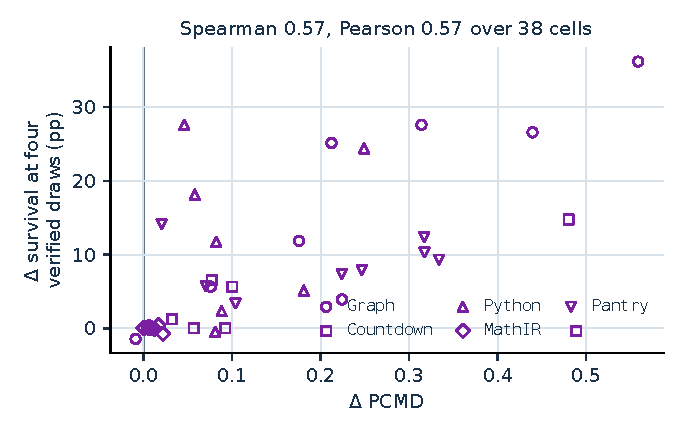
\includegraphics[width=0.62\linewidth]{figures/withdrawal_pmd_agreement.pdf}
  \caption{\textbf{Diversity gains correlate with survival gains after a withdrawal.} Each mark is one replay--fresh-objective contrast in a domain, scale and level. The horizontal axis is the terminal \pmd{} difference; the vertical axis is the percentage-point survival difference at four verified draws, averaged equally over eligible seed-specific contrasts. Survival uses jointly eligible prompt--group pairs within each seed. Marker shape identifies the domain; zero lines mark no change. The 38 comparisons have Pearson and Spearman correlations of $.57$; points show estimates without intervals. The association is descriptive, and the two metrics need not use the same eligible population.}
  \label{fig:withdrawal-pmd-agreement}
\end{figure}

\subsection{Two withdrawals at once}
\label{app:withdrawal-severity}
We next remove two binding options at once. Of the 29{,}213 pairs of binding
single withdrawals, 26{,}927 retain at least one certified mode and enter the
survival comparison. For \texttt{Graph}, \texttt{Countdown}, \texttt{Python} and \texttt{PantryPlan},
a certified mode survives the pair exactly when it survives both individual
withdrawals. \texttt{MathIR} can differ: removing two actions can eliminate every
realization of a state path even when either action alone can be removed.
Re-enumerating the reduced menus shows that no such case occurs here: for all
1{,}344 \texttt{MathIR} pairs, including those that leave no certified mode,
the surviving set equals the intersection of the two single-withdrawal sets.

\begin{table}[!htbp]
\centering
\caption{\textbf{Two withdrawals retain survival gains in \texttt{Graph}, \texttt{Python} and \texttt{PantryPlan}.} Entries are replay--fresh-objective differences in percentage points at two (@2) or four (@4) verified draws. One uses binding single options; Two uses binding pairs with a feasibility certificate. Their eligible prompt populations can differ. Estimates pool jointly eligible groups. Brackets are pointwise 95\% paired prompt-bootstrap intervals with the clustering in Table~\ref{tab:withdrawal-contrasts}.}
\label{tab:withdrawal-severity}
\scriptsize
\setlength{\tabcolsep}{3pt}
\begin{tabular}{llrrrr}
\toprule
Domain & Arm & One @2 & One @4 & Two @2 & Two @4 \\
\midrule
\texttt{Graph} & Re:Dr & $10.51$ & $19.65$ $[15.61, 23.82]$ & $10.02$ & $23.65$ $[19.14, 28.25]$ \\
\texttt{Graph} & Re:Max & $6.62$ & $10.99$ $[8.25, 13.81]$ & $5.93$ & $12.51$ $[9.37, 15.69]$ \\
\texttt{Countdown} & Re:Dr & $6.52$ & $9.58$ $[6.81, 12.63]$ & $3.29$ & $6.11$ $[0.87, 12.22]$ \\
\texttt{Countdown} & Re:Max & $-1.25$ & $0.10$ $[-2.62, 2.78]$ & $-5.53$ & $-4.87$ $[-11.80, 0.76]$ \\
\texttt{Python} & Re:Dr & $4.09$ & $7.67$ $[6.82, 8.58]$ & $5.37$ & $10.10$ $[8.77, 11.55]$ \\
\texttt{Python} & Re:Max & $3.85$ & $5.68$ $[4.80, 6.64]$ & $5.64$ & $8.16$ $[6.79, 9.64]$ \\
\texttt{MathIR} & Re:Dr & $0.12$ & $0.14$ $[0.00, 0.30]$ & $0.18$ & $0.20$ $[0.01, 0.45]$ \\
\texttt{MathIR} & Re:Max & $0.03$ & $0.09$ $[-0.01, 0.21]$ & $0.04$ & $0.12$ $[-0.01, 0.29]$ \\
\texttt{PantryPlan} & Re:Dr & $4.36$ & $9.78$ $[8.90, 10.65]$ & $2.85$ & $7.23$ $[6.51, 7.95]$ \\
\texttt{PantryPlan} & Re:Max & $3.12$ & $6.61$ $[5.83, 7.39]$ & $2.03$ & $4.94$ $[4.35, 5.57]$ \\
\bottomrule
\end{tabular}
\end{table}

Two withdrawals retain less certified support on average
(Table~\ref{tab:withdrawal-inventory}). Re:Dr's pooled survival gain at four
verified draws rises in \texttt{Graph}, \texttt{Python} and \texttt{MathIR}, and falls in \texttt{Countdown} and
\texttt{PantryPlan}. \texttt{Countdown} Level 1 starts with only 4.5 certified modes per prompt;
\texttt{PantryPlan} Level 1 retains only 18\% of its certified modes under a binding pair.
These support differences coincide with the smaller gains but do not
establish their cause. Across domain--scale--level--objective comparisons,
25 of 39 point estimates are positive at four verified draws,
compared with 28 of 39 for single withdrawals.

\subsection{Decoding settings as a substitute}
\label{app:withdrawal-decoding}
Can a better decoding setting give an ordinary policy the same survival?
We evaluate binding Level-1 withdrawals on 128 prompts per domain, using the
separate Qwen2.5-0.5B cohort trained for twelve passes in
App.~\ref{app:decoding-objection}. Its replay variant combines separate mass
and within-buffer balancing terms with novelty and semantic-entropy shaping;
it differs from Re:Dr in both objective and training duration. Five seeds per
arm are evaluated at 11 settings: six temperatures from $.5$ to $2.0$,
three settings with larger groups, and two with top-$p=.95$. Larger groups
increase $K$ from 8 to 32, but use two groups rather than four: total responses
per prompt double from 32 to 64. The reference is $T=1$, top-$p=1$, and four
groups of eight. For each domain, we select the control setting with the
highest four-verified-draw survival on these evaluation prompts, while replay
keeps the reference setting.

\begin{table}[!htbp]
\centering
\caption{\textbf{Replay survival exceeds the selected control setting in all five domains.} Survival at four verified draws is expressed as percentages. Control, Control grid and Replay are equal-seed means on each setting's own eligible groups; the grid column gives the control range and Best its maximizing temperature. $\Delta$ instead pools jointly eligible groups for reference replay minus selected control, so it need not equal the difference of the displayed means. Brackets are pointwise 95\% intervals from 20{,}000 paired prompt-bootstrap replicates, keeping all groups and five seeds of a prompt together. The selected setting stays fixed in the bootstrap; intervals condition on that selection and the seeds.}
\label{tab:withdrawal-decoding}
\scriptsize
\setlength{\tabcolsep}{3pt}
\begin{tabular}{lrrcrr}
\toprule
Domain & Control & Control grid & Best & Replay & $\Delta$ vs best \\
\midrule
\texttt{Graph} & 58.61 & 58.59--58.85 & $T{=}2$ & 95.91 & $36.97$ $[35.53, 38.42]$ \\
\texttt{Countdown} & 15.49 & 12.57--16.16 & $T{=}1.6$ & 40.09 & $28.87$ $[18.98, 38.87]$ \\
\texttt{Python} & 70.54 & 70.36--70.54 & $T{=}0.5$ & 77.56 & $8.33$ $[7.15, 9.69]$ \\
\texttt{MathIR} & 72.23 & 72.18--72.55 & $T{=}2$ & 73.60 & $1.37$ $[0.61, 2.30]$ \\
\texttt{PantryPlan} & 50.65 & 50.02--51.79 & $T{=}2$ & 64.09 & $12.73$ $[10.22, 15.31]$ \\
\bottomrule
\end{tabular}
\end{table}

Control survival spans at most 3.6 percentage points across the grid.
The paired replay gains range from 1.4 to 37.0 points, with all five
pointwise intervals above zero. Every selected control setting changes only the
temperature, keeping eight-response groups and top-$p=1$. The tested decoding
changes therefore do not close the survival gap in this cohort. Because each
control setting is selected on the evaluation prompts, the control's survival
is, if anything, optimistic for new prompts. Finite samples cannot show that
the missing alternative modes have zero probability under the control.

\subsection{Recovery after a withdrawal}
\label{app:withdrawal-recovery}
Recovery is evaluated at the Level-1 Qwen2.5-0.5B terminal Dr.GRPO and Re:Dr
checkpoints from two matched training seeds in each of five domains. Each domain has 32 test and 16 temperature-calibration prompts in a
disjoint split. Prompts without a binding withdrawal that retains a certified
mode are excluded, leaving 28 test and 15 calibration prompts in \texttt{Countdown} and all
prompts elsewhere. Up to four binding options per test prompt give
533 distinct withdrawals, shared by both arms and seeds.

Each initial portfolio contains eight responses. Ordinary sampling uses its
terminal evaluation group at $T=1$. The temperature strategy generates a group
at the temperature in $\{.7,1.0,1.3\}$ maximizing mean survival on the
calibration prompts. The diversity-prompt strategy generates the eight
responses sequentially, with the preceding responses included in each request.
All strategies share the same recovery procedure. If no initial mode survives,
the model generates one response per call at $T=1$, for up to eight calls,
with the revised task, the initial portfolio and previous failed attempts in
context. Recovery stops at the first verified response whose mode survives the
withdrawal.

Survival uses the mode predicates defined above. In \texttt{MathIR}, a retained or newly
generated state path can count as surviving even if realizing it under the
reduced menu requires a different action sequence. \texttt{PantryPlan} responses are
six-bit ingredient-support masks projected onto verified quantities by the
environment (App.~\ref{app:prompt-pantry}); survival is evaluated on the resulting
support key. These outcomes therefore measure whether a mode remains feasible,
not whether the original response text can be reused unchanged.

\begin{table}[!htbp]
\centering
\caption{\textbf{Replay improves ordinary and temperature-tuned recovery in every domain.} Saved is the percentage of withdrawals with a surviving initial mode; By 8 also counts those resolved within eight additional responses. Calls is the mean additional response count, with zero for initial survival and eight for unresolved cases. Each row pools the same withdrawals over two matched seeds. Fresh is Dr.GRPO and Replay is Re:Dr; the three strategies differ only in initial portfolio generation.}
\label{tab:withdrawal-recovery}
\scriptsize
\setlength{\tabcolsep}{3pt}
\begin{tabular}{llrrrrrr}
\toprule
Domain & Strategy & Fresh saved & Fresh by 8 & Fresh calls & Replay saved & Replay by 8 & Replay calls \\
\midrule
\texttt{Graph} & Ordinary & 15.62 & 22.66 & 6.38 & 83.20 & 91.02 & 1.01 \\
\texttt{Graph} & Tuned temperature & 15.62 & 20.31 & 6.55 & 77.34 & 89.06 & 1.36 \\
\texttt{Graph} & Diversity prompt & 29.69 & 30.47 & 5.58 & 62.50 & 74.61 & 2.44 \\
\texttt{Countdown} & Ordinary & 2.70 & 2.70 & 7.78 & 9.46 & 10.81 & 7.23 \\
\texttt{Countdown} & Tuned temperature & 2.70 & 2.70 & 7.78 & 9.46 & 13.51 & 7.05 \\
\texttt{Countdown} & Diversity prompt & 2.70 & 2.70 & 7.78 & 5.41 & 9.46 & 7.41 \\
\texttt{Python} & Ordinary & 14.06 & 14.06 & 6.88 & 69.92 & 77.73 & 2.21 \\
\texttt{Python} & Tuned temperature & 14.06 & 14.06 & 6.88 & 71.88 & 75.78 & 2.12 \\
\texttt{Python} & Diversity prompt & 14.06 & 14.06 & 6.88 & 62.50 & 67.97 & 2.79 \\
\texttt{MathIR} & Ordinary & 38.39 & 44.20 & 4.60 & 58.93 & 65.18 & 2.92 \\
\texttt{MathIR} & Tuned temperature & 37.05 & 45.09 & 4.61 & 63.84 & 67.86 & 2.67 \\
\texttt{MathIR} & Diversity prompt & 41.07 & 45.09 & 4.58 & 47.32 & 53.57 & 3.85 \\
\texttt{PantryPlan} & Ordinary & 31.25 & 31.64 & 5.48 & 47.66 & 52.34 & 4.04 \\
\texttt{PantryPlan} & Tuned temperature & 31.25 & 44.53 & 4.81 & 53.12 & 62.11 & 3.38 \\
\texttt{PantryPlan} & Diversity prompt & 56.64 & 58.20 & 3.39 & 33.98 & 45.70 & 4.71 \\
\bottomrule
\end{tabular}
\end{table}


\begin{table}[!htbp]
\centering
\caption{\textbf{Recovery benefits depend on the initial portfolio strategy.} Entries are paired Re:Dr--Dr.GRPO differences on the same withdrawals under each strategy. Saved and By 8 are percentage points; Calls is additional responses. Brackets are pointwise 95\% intervals from 20{,}000 paired prompt-bootstrap replicates. Each prompt's withdrawals and both training seeds move together; intervals condition on those two matched training seeds.}
\label{tab:withdrawal-recovery-contrast}
\scriptsize
\setlength{\tabcolsep}{3pt}
\begin{tabular}{llrrr}
\toprule
Domain & Strategy & $\Delta$ saved & $\Delta$ by 8 & $\Delta$ calls \\
\midrule
\texttt{Graph} & Ordinary & $67.58$ $[57.81, 76.56]$ & $68.36$ $[59.38, 76.95]$ & $-5.37$ $[-6.05, -4.65]$ \\
\texttt{Graph} & Tuned temperature & $61.72$ $[51.95, 71.09]$ & $68.75$ $[61.33, 75.78]$ & $-5.20$ $[-5.84, -4.52]$ \\
\texttt{Graph} & Diversity prompt & $32.81$ $[21.09, 44.14]$ & $44.14$ $[34.77, 53.12]$ & $-3.14$ $[-3.95, -2.30]$ \\
\texttt{Countdown} & Ordinary & $6.76$ $[1.35, 13.89]$ & $8.11$ $[1.43, 16.18]$ & $-0.55$ $[-1.12, -0.11]$ \\
\texttt{Countdown} & Tuned temperature & $6.76$ $[1.35, 13.89]$ & $10.81$ $[3.33, 19.32]$ & $-0.73$ $[-1.35, -0.21]$ \\
\texttt{Countdown} & Diversity prompt & $2.70$ $[0.00, 6.58]$ & $6.76$ $[1.32, 13.64]$ & $-0.38$ $[-0.76, -0.06]$ \\
\texttt{Python} & Ordinary & $55.86$ $[44.92, 65.23]$ & $63.67$ $[51.56, 74.22]$ & $-4.67$ $[-5.45, -3.76]$ \\
\texttt{Python} & Tuned temperature & $57.81$ $[46.88, 67.19]$ & $61.72$ $[50.39, 71.48]$ & $-4.76$ $[-5.54, -3.87]$ \\
\texttt{Python} & Diversity prompt & $48.44$ $[37.11, 59.38]$ & $53.91$ $[41.80, 65.62]$ & $-4.09$ $[-4.99, -3.14]$ \\
\texttt{MathIR} & Ordinary & $20.54$ $[11.16, 30.09]$ & $20.98$ $[12.71, 29.82]$ & $-1.68$ $[-2.37, -1.02]$ \\
\texttt{MathIR} & Tuned temperature & $26.79$ $[18.26, 35.65]$ & $22.77$ $[13.89, 32.27]$ & $-1.94$ $[-2.66, -1.28]$ \\
\texttt{MathIR} & Diversity prompt & $6.25$ $[-4.09, 16.67]$ & $8.48$ $[-0.46, 18.26]$ & $-0.73$ $[-1.50, 0.03]$ \\
\texttt{PantryPlan} & Ordinary & $16.41$ $[8.20, 25.39]$ & $20.70$ $[11.72, 30.47]$ & $-1.44$ $[-2.18, -0.76]$ \\
\texttt{PantryPlan} & Tuned temperature & $21.88$ $[13.28, 31.25]$ & $17.58$ $[10.94, 24.61]$ & $-1.43$ $[-2.00, -0.91]$ \\
\texttt{PantryPlan} & Diversity prompt & $-22.66$ $[-31.25, -13.67]$ & $-12.50$ $[-21.88, -2.73]$ & $1.32$ $[0.55, 2.05]$ \\
\bottomrule
\end{tabular}
\end{table}

With ordinary or temperature-tuned initial portfolios, replay resolves more
withdrawals and uses fewer recovery responses in every domain. All ten
resolution contrasts and all ten response-count contrasts have pointwise
intervals excluding zero. With ordinary initial portfolios, replay needs
0.55 to 5.37 fewer recovery responses per withdrawal. Summed over all
three strategies and both seeds, replay uses 9{,}872 recovery responses and
the control uses 18{,}335. These totals cover recovery only, excluding initial
portfolios and temperature calibration, and response counts do not account for
token or context lengths or for training compute.

The diversity prompt increases the control's initial survival in \texttt{Graph} and
\texttt{PantryPlan} relative to ordinary sampling, with intervals above zero. For
replay, it lowers the initial-survival point estimate in every domain. The
intervention changes both the request for alternatives and the accumulated
context, and this design does not separate their effects. With both arms using
the diversity prompt, \texttt{PantryPlan} favors the control by 22.66 points of initial survival and 12.50 points of
resolution by eight calls. Replay's initial-survival difference is positive
in the other four domains, ranging from 2.7 to 48.4 points, although the
\texttt{Countdown} and \texttt{MathIR} intervals include zero. \texttt{PantryPlan}'s six-bit response format
permits enumerating support masks, but this comparison does not establish that
enumerability explains the reversal.

\paragraph{Interpretation and limits.} In \texttt{Graph}, \texttt{Countdown}, \texttt{Python} and \texttt{PantryPlan},
Re:Dr's broader four-draw portfolios accompany larger survival gains than in
\texttt{MathIR}. The positive association with \pmd{} is descriptive. Fixing the number
of verified draws conditions on jointly eligible groups; it does not fix policy
accuracy, and eligibility can change with the draw budget. An option enters
the analysis only when a certified mode survives it; where the certified count
is a lower bound on the verifier's support, some excluded options may also be
feasible. The interventions cover single and paired withdrawals rather than
arbitrary task revisions. Recovery outcomes rest on domain-specific mode
predicates, and \texttt{PantryPlan}'s ordering reverses under the diversity prompt. Finally, the intervals quantify prompt-sampling uncertainty within
the observed training cohorts; they do not estimate variability over new
training seeds.


\clearpage
\phantomsection
\begin{center}\large\textbf{Part V. Fixed deployments}\end{center}
\addcontentsline{toc}{part}{Part V. Fixed deployments}

\section{Inference-Only Concentration in a Hosted Model}
\label{app:hosted-concentration}

This exploratory evaluation measures the current output distribution of
GPT-5.6 Sol under the inherited \mb{} interface. It is separate from the matched
training interventions: it adds no frontier-model training, replay comparison,
or controlled model-size contrast. Only the completed, audited deployment
enters these tables.

\paragraph{Protocol and provenance.}
The September 11, 2026 run uses the Azure deployment \texttt{gpt-5.6-sol}; saved
provider headers identify snapshot \texttt{gpt-5.6-sol-2026-07-09}. Each of the
five domains contributes 128 held-out prompts at each of three levels. Eight
stateless requests per prompt yield 15,360 responses. Requests use medium
reasoning, an 8,192-token output limit, no tools and no conversation state.
The service returns temperature $1.0$ and top-$p$ $.98$; neither setting was
overridden. These settings and the hosted natural-language interface differ
from the local training evaluation's token-level grammar constraints.

Level 1 uses the native E118 evaluation splits retained in E124. Level 2 uses
the frozen matched r5 construction; Level 3 uses the matched v3 construction
admitted by the completed canonical v3 confirmation. Level 3 is an exploratory
test extension here, not a third level of the paper's training intervention.
All cells use the multi-answer split. The Level-2/Level-3 support histograms
match a separate fixed-reference Level-1 confirmation reserve, which differs
from the native Level-1 split in Graph, Countdown and Python. Prompts differ
across levels and are not paired by row index. Calibration against small-model
references does not guarantee increasing difficulty for this hosted model.

Exact prompts, dataset identities and hashes, requests, provider-exposed
responses, grades, retry receipts, usage and verifier snapshots are retained
in the experiment's evidence directory. All 15,360 intended samples completed,
with distinct response identifiers; 107 failed API attempts were retained and
recovered by retries. Provider random-number independence and hidden reasoning
contents cannot be audited from the exposed responses.

\begin{table}[!htbp]
  \centering
  \caption{\textbf{Hosted correctness and concentration under strict grading.}
  GPT-5.6 Sol, with medium reasoning. Each level weights five domains equally.
  M and P are \texttt{mean@8} and \texttt{pass@8} (\%); D is raw
  \texttt{distinct@8}. C is the percentage of within-prompt correct pairs
  sharing a mode, pair weighted within each domain. Brackets give pointwise
  95\% intervals from whole-prompt resampling.}
  \label{tab:hosted-levels}
  \small
  \begin{tabular}{@{}rrrrl@{}}
    \toprule
    Level & M & P & D & C (95\% interval) \\
    \midrule
    1 & 83.0 & 95.8 & 1.71 & 74.0 [71.9, 76.1] \\
2 & 62.9 & 77.5 & 1.16 & 82.3 [80.3, 84.4] \\
3 & 68.7 & 80.3 & 1.18 & 84.5 [82.8, 86.2] \\
\bottomrule

  \end{tabular}
\end{table}

\paragraph{Metrics and uncertainty.}
Per-response correctness is \texttt{mean@8} in this paper (called
\texttt{pass@1} in the hosted report). Raw \texttt{distinct@8} counts verified
keys across eight draws, including zero for unsolved prompts. For prompt $x$,
let $c_x$ be its number of correct draws and $n_{xc}$ its count for correct
key $c$. The within-cell correct-pair collision estimate is
\[
  \widehat C=
  \frac{\sum_x\sum_c\binom{n_{xc}}{2}}
       {\sum_x\binom{c_x}{2}}.
\]
It describes concentration conditional on successful draws, with prompts
weighted by their number of correct pairs. Level summaries average the five
domain estimates equally. When the certified correct-key count $m_x$ is
available, a uniform-correct-key reference replaces the numerator by
$\sum_x\binom{c_x}{2}/m_x$. This differs from a uniform-action baseline and
is a descriptive reference, not a normative sampling requirement. Countdown's
verifier accepts modes beyond its enumerated binary-expression library,
including unary negation, so its total support is unknown and this reference
is omitted. Intervals use 2,000 whole-prompt bootstrap replicates, seed
20260911, resampling within each domain and level and keeping all eight draws
together. They are pointwise descriptive intervals.

\begin{table}[!htbp]
  \centering
  \caption{\textbf{GPT-5.6 Sol under strict executable grading.}
  Every cell contains 128 prompts and 1,024 responses. M and P are
  \texttt{mean@8} and \texttt{pass@8} (\%); D is \texttt{distinct@8}.
  C is correct-pair collision (\%, with 95\% prompt-bootstrap interval);
  U is the uniform-correct-key collision reference (\%).}
  \label{tab:hosted-strict}
  \small
  \setlength{\tabcolsep}{4pt}
  \begin{tabular}{@{}rlrrrrr@{}}
    \toprule
    Level & Domain & M & P & D & C (95\% interval) & U \\
    \midrule
    1 & Graph & 99.2 & 100.0 & 1.30 & 89.7 [86.3, 92.8] & 18.3 \\
1 & Countdown & 86.1 & 98.4 & 1.77 & 71.2 [66.1, 75.9] & -- \\
1 & Python & 40.4 & 90.6 & 1.11 & 81.8 [76.9, 87.2] & 0.8 \\
1 & MathIR & 89.3 & 89.8 & 1.38 & 80.3 [75.4, 85.0] & 20.0 \\
1 & PantryPlan & 100.0 & 100.0 & 3.00 & 46.9 [42.2, 51.5] & 6.5 \\
\midrule
2 & Graph & 99.3 & 100.0 & 1.48 & 83.3 [79.6, 87.0] & 18.9 \\
2 & Countdown & 65.4 & 86.7 & 1.57 & 64.7 [59.0, 70.6] & -- \\
2 & Python & 8.5 & 11.7 & 0.12 & 100.0 [100.0, 100.0] & 0.7 \\
2 & MathIR & 86.2 & 93.0 & 0.93 & 100.0 [100.0, 100.0] & 20.0 \\
2 & PantryPlan & 55.3 & 96.1 & 1.72 & 63.6 [56.8, 70.3] & 6.9 \\
\midrule
3 & Graph & 100.0 & 100.0 & 1.16 & 95.1 [92.4, 97.3] & 19.0 \\
3 & Countdown & 71.2 & 89.8 & 1.38 & 76.4 [71.1, 81.8] & -- \\
3 & Python & 9.4 & 14.1 & 0.14 & 100.0 [100.0, 100.0] & 0.9 \\
3 & MathIR & 97.7 & 97.7 & 0.98 & 100.0 [100.0, 100.0] & 20.0 \\
3 & PantryPlan & 65.3 & 100.0 & 2.22 & 51.0 [45.3, 57.3] & 6.8 \\
\bottomrule

  \end{tabular}
\end{table}

\paragraph{Formatting sensitivity.}
Strict grades remain primary. A secondary typography normalizer was introduced
after inspecting the first 15 responses. It fixes a frozen set of presentation
conventions, including escaped Python/LaTeX syntax, and reuses the original
executable validators without repairing calculations or program logic.
It recovers 2,580 additional verified outputs; strict successes and their keys
are retained. This is a post hoc diagnostic, not a replacement benchmark.
All 3,072 primary Python responses passed an independent serial recheck with
no grade changes. One cold-start timeout in the secondary grading cache was
reconciled with repeated serial verification; the original cache and correction
audit remain preserved.

\begin{table}[!htbp]
  \centering
  \caption{\textbf{Post hoc formatting-normalized diagnostic.}
  Same samples and metric definitions as Table~\ref{tab:hosted-strict}, with
  fixed presentation normalization before executable verification. The strict
  table remains primary; normalization was designed after the first 15
  responses.}
  \label{tab:hosted-normalized}
  \small
  \setlength{\tabcolsep}{4pt}
  \begin{tabular}{@{}rlrrrrr@{}}
    \toprule
    Level & Domain & M & P & D & C (95\% interval) & U \\
    \midrule
    1 & \texttt{Graph} & 99.2 & 100.0 & 1.30 & 89.7 [86.3, 92.8] & 18.3 \\
1 & \texttt{Countdown} & 99.9 & 100.0 & 1.93 & 67.9 [63.3, 72.4] & -- \\
1 & \texttt{Python} & 92.4 & 100.0 & 1.41 & 85.6 [82.3, 88.8] & 1.4 \\
1 & \texttt{MathIR} & 89.3 & 89.8 & 1.38 & 80.3 [75.4, 85.0] & 20.0 \\
1 & \texttt{PantryPlan} & 100.0 & 100.0 & 3.00 & 46.9 [42.2, 51.5] & 6.5 \\
\midrule
2 & \texttt{Graph} & 99.3 & 100.0 & 1.48 & 83.3 [79.6, 87.0] & 18.9 \\
2 & \texttt{Countdown} & 98.5 & 100.0 & 1.99 & 63.9 [59.5, 68.4] & -- \\
2 & \texttt{Python} & 60.7 & 99.2 & 1.12 & 94.8 [91.9, 97.2] & 1.1 \\
2 & \texttt{MathIR} & 86.2 & 93.0 & 0.93 & 100.0 [100.0, 100.0] & 20.0 \\
2 & \texttt{PantryPlan} & 71.3 & 100.0 & 1.96 & 64.0 [58.1, 69.6] & 6.8 \\
\midrule
3 & \texttt{Graph} & 100.0 & 100.0 & 1.16 & 95.1 [92.4, 97.3] & 19.0 \\
3 & \texttt{Countdown} & 99.0 & 100.0 & 1.70 & 75.7 [71.2, 80.1] & -- \\
3 & \texttt{Python} & 56.5 & 98.4 & 1.09 & 94.3 [90.8, 97.2] & 1.0 \\
3 & \texttt{MathIR} & 97.7 & 97.7 & 0.98 & 100.0 [100.0, 100.0] & 20.0 \\
3 & \texttt{PantryPlan} & 75.2 & 100.0 & 2.35 & 53.0 [47.3, 58.9] & 6.7 \\
\bottomrule

  \end{tabular}
\end{table}

\paragraph{Concentration and level.}
The strict five-domain collision average is $74.0\%$, $82.3\%$ and $84.5\%$
at Levels 1--3; the normalized diagnostic gives $74.1\%$, $81.2\%$ and
$83.6\%$. This aggregate pattern is not a monotonic law within domains.
Graph collision is $89.7\%$, $83.3\%$, then $95.1\%$; normalized PantryPlan
collision is $46.9\%$, $64.0\%$, then $53.0\%$. Normalized overall correctness
also rebounds from $83.2\%$ at Level 2 to $85.7\%$ at Level 3. Thus a higher
level label is not equivalent to a measured increase in difficulty for this
model, and raw distinct-mode counts also change with correctness and support.

Level-3 Graph separates concentration from failed responses particularly
clearly: all 1,024 outputs verify, eight draws produce $1.16$ distinct keys
on average, and 3,407 of 3,584 correct pairs share a key ($95.1\%$). The
uniform-correct-key reference is $19.0\%$; the excess is $76.1$ percentage
points (95\% interval $[73.5,78.3]$). Graph was selected after the GPT run for
this illustration because its correctness is high, support is certified and
formatting normalization changes no scores; both tables report all domains.

\paragraph{Interface and claim limits.}
Level-2/Level-3 MathIR instructions prescribe moving the right-side variable
term left, removing the constant and then dividing. Python instructions
suggest a nested small-divisor conditional chain, and PantryPlan instructions
prefer particular ingredient families. These preferences can concentrate the
very keys being measured. In addition, Level-1 PantryPlan requests a support
mask whose quantities are supplied by a trusted projection; Levels 2--3 ask
the model to provide quantities. MathIR verifies symbolic action compliance,
which can reject a numerically valid shortcut that omits a required symbolic
step. Neither these failures nor the cross-level differences isolate numerical
reasoning ability. Canonical keys describe executed outputs, not hidden
reasoning strategies. Eight draws cannot establish that an unseen mode has
zero probability. The evidence supports concentration under the specified
prompts and deployment configuration; it identifies neither a training cause
nor a causal difficulty or model-size effect.

\paragraph{Reproduction record.}
The source record is
\path{artifacts/frontier_modebench_gpt56sol_20260911/summary.json}.
Its hash, complete cell statistics and run settings are copied into
\path{results/frontier_hosted_20260911.json}; adjacent generated table bodies
supply the displayed values. The evidence directory also retains
\path{completion_audit.json}, \path{prompt_contract_audit.json}, the original
requests and responses, and \path{interpretation_notes.md}. Hosted-model
results are separate from the training-checkpoint archive and its matched-seed
comparisons.


\subsection{Hosted concentration on the success-conditional axis}
\label{app:hosted-mode-diversity}

Table~\ref{tab:hosted-cohort-mode-diversity} reports promptwise \pmd{}
under strict grading and the original task wording. Within each cell it
averages equally over prompts with at least two verified responses; a cell
is reportable when at least thirty prompts qualify. The collision tables
above instead weight prompts by their number of correct pairs. For GPT-5.6
Sol under strict grading, $1-\widehat C$ and promptwise \pmd{} summarize
the same responses with different weights (App.~\ref{app:metric-sampling}).
Fig.~\ref{fig:hosted-verified-breadth} shows the corresponding strict,
original-wording cell estimates in its diversity row. Its accuracy row uses
formatting normalization and revised Opus~5 \texttt{Python} wording, so the two rows
have different grading and, for that deployment and domain, different
prompt conditions.

For GPT-5.6 Sol, strict \texttt{MathIR} \pmd{} is $.000$ at Levels~2 and~3: none of
the 110 and 125 eligible prompts, respectively, contains two different
verified keys. Level-3 \texttt{Graph} has \pmd{} $.049$, although its prompts admit
between four and twelve valid colorings. \texttt{PantryPlan} has higher diversity,
with \pmd{} $.531$, $.386$ and $.455$ across the three levels. \texttt{Python} at
Levels~2 and~3 has only 14 and 15 eligible prompts out of 128, below the
thirty-prompt reporting threshold. These missing entries reflect strict
formatting failures, including LaTeX-escaped Python; this deployment has no
provider refusals in those cells. Opus~5's corresponding missing entries
have a different cause: 1,021 and 1,024 of its 1,024 responses are refusals.

\paragraph{Level 4.}
The GPT-5.6 Sol Level-4 points in Fig.~\ref{fig:base-levels-all-scales}
average to $.181$ across $5$ domains,
using the pair-pooled $1-\widehat C$ statistic and formatting normalization.
This evaluation uses the direct OpenAI service, whereas Levels~1--3 use
Azure. The deployments may differ, so their contrast does not isolate a
level effect. \texttt{Python} is particularly sensitive to grading: strict grading
verifies two of 1,024 responses, compared with 675 after normalization.
Normalization changes the correct-response population on which diversity
is measured. This difference measures sensitivity to output formatting;
it does not establish correctness for the remaining responses.

\paragraph{Concentration across deployments.}
Under strict grading, macro \pmd{} ranges from $.142$ for Claude Opus~5 to
$.320$ for DeepSeek V4 Pro across the seven deployments. They use the thirteen domain--level cells that
are reportable for every deployment, excluding \texttt{Python} at Levels~2 and~3.
The transformed summaries $\neff=1/(1-\text{macro }\pmd)$ range from
$1.17$ to $1.47$. These are transforms of the mean diversity,
not averages of per-cell effective mode counts or bounds on unseen modes.
At the largest observed macro, the corresponding mean probability of
repeating a correct mode is about $.68$ under these prompt and cell weights.

\texttt{MathIR} defines modes by canonical derivation paths; the other domains use
alternative output structures. Removing the three \texttt{MathIR} cells raises every
deployment's macro. Across the ten remaining common cells, the largest
transformed summary is $1.58$, for Kimi~K3. \texttt{Python}
contributes only Level~1 to this comparison, so this is an equal-cell mean,
not an equal-domain mean over four domains. The low diversity summaries
therefore persist without \texttt{MathIR}, although their magnitudes depend on the
mode definitions and averaging population.

Averaging each deployment over its own reportable cells instead changes the
ranking: DeepSeek V4 Pro has $.280$ across its fifteen cells and falls below
Kimi~K3. Domain rankings also differ: GPT-5.4 and Kimi~K3 have higher \texttt{Python}
diversity, while DeepSeek V4 Pro has higher \texttt{Graph} diversity. Every deployment's
per-level mean is lower at Level~3 than at Level~1, although Level~2 does not
always lie between them. Fig.~\ref{fig:frontier-level-grid} shows the
normalized cohort, one deployment per row.

\begin{table}[!htbp]
  \centering
  \caption{\textbf{Seven hosted deployments have low diversity among correct solutions.}
  Strict grading, original wording, 128 prompts per domain--level cell and
  eight stateless requests per prompt. Within-cell \pmd{} weights eligible
  prompts equally. Macro \pmd{} averages the same thirteen cells for every
  deployment, omitting \texttt{Python} L2/L3; $\neff$ transforms that macro.
  L1--L3 columns average each deployment's own reportable cells: five domains
  per level, except four at L2/L3 for GPT-5.6 Sol and Opus~5. Thus the macro
  is not the mean of those three columns. A cell requires thirty prompts
  with at least two verified responses. Entries are point estimates.}
  \label{tab:hosted-cohort-mode-diversity}
  \small
  \begin{tabular}{lccccc}
    \toprule
    & & & \multicolumn{3}{c}{Macro \pmd{} by level} \\
    \cmidrule(lr){4-6}
    Deployment & Macro \pmd{} & $\neff$ & L1 & L2 & L3 \\
    \midrule
    Kimi K3 & .311 & 1.45 & .374 & .307 & .253 \\
DeepSeek V4 Pro & .280 & 1.39 & .289 & .319 & .232 \\
GPT-5.4 & .269 & 1.37 & .338 & .247 & .224 \\
GPT-5.6 Sol & .226 & 1.29 & .256 & .229 & .183 \\
Grok 4.3 & .209 & 1.26 & .275 & .179 & .171 \\
Claude Opus 4.8 & .205 & 1.26 & .217 & .229 & .168 \\
Claude Opus 5 & .142 & 1.17 & .140 & .164 & .121 \\
    \bottomrule

  \end{tabular}
\end{table}

\paragraph{Level comparisons also change prompt guidance.}
The Level-2 and Level-3 system messages add strategy guidance to \texttt{MathIR},
\texttt{Python} and \texttt{PantryPlan}: an algebraic isolation order, a nested small-divisor
chain and a preference over ingredient families. Level~1 lacks this guidance.
In the normalized original-wording cohort, pair-pooled $1-\widehat C$ falls
from Level~1 to Level~3 by $.115$ on average across the
$20$ measured deployment--domain pairs in these domains,
compared with $.048$ across the $14$ pairs in
\texttt{Graph} and \texttt{Countdown}. Averaging the two unguided domains within each model,
$7$ of $7$ deployments also decline.
The guided and unguided domains also differ in their tasks and solution
spaces, so this comparison does not estimate the effect of guidance.

The prompt ablations test the effect of guidance directly, under narrower conditions.
Removing \texttt{MathIR} guidance from the local 0.5B checkpoints leaves observed
\pmd{} at $.000$ under both wordings
(App.~\ref{app:prompt-hint-ablation}). The separate 64-draw hosted study
finds higher Level-2 \texttt{MathIR} diversity under neutral wording for both GPT
deployments at fixed correct-draw budgets, with intervals excluding zero;
Grok's intervals include zero (App.~\ref{app:hosted-discovery-complete}).
These comparisons condition on jointly eligible prompts and do not match
overall accuracy. The local and hosted results come from different models and
evaluation populations, so their responses to wording need not agree. Cross-level narrowing describes
concentration under the specified prompts; it does not isolate task
difficulty from prompting or deployment differences.


% Render this retained display inside its generated numerical appendix.
\AddToHookNext{file/after/gpt56_temperature_curve_20260911_appendix.tex}{%
\begin{figure}[!htbp]
  \centering
  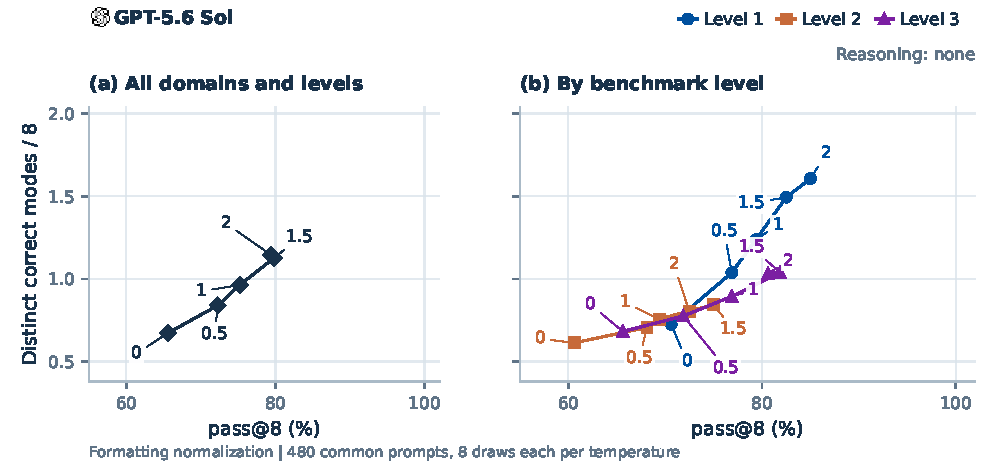
\includegraphics[width=.98\linewidth]{figures/gpt56_temperature_curve.pdf}
  \caption{\textbf{Nonzero temperatures yield greater observed eight-draw coverage.}
  GPT-5.6 Sol with reasoning \texttt{none}, typography normalization, and the same
  480 prompts at each of five temperatures (32 per domain--level cell, eight
  responses each). Left: an equal mean over all 15 domain--level cells; right:
  equal means over five domains at each level, identified by color and marker.
  The horizontal axis is empirical \texttt{pass@8}; the vertical axis averages
  distinct correct solution modes per eight responses, including unsolved prompts
  as zero. Labels give requested temperatures; segments connect measured point
  estimates in temperature order. Table~\ref{tab:gpt56-temperature} gives
  95\% whole-prompt bootstrap intervals. Mode counts depend on
  success and correct-answer variation and need not track \texttt{pass@8}.}
  \label{fig:gpt56-temperature-curve}
\end{figure}
}

\section{Comparison across Hosted Deployments}
\label{app:hosted-comparison}

Figure~\ref{fig:hosted-verified-breadth} compares accuracy and success-conditional
solution-mode diversity across hosted deployments. Its accuracy row uses a
common formatting normalizer and the revised Opus 5 \texttt{Python} instructions at
each level; hollow marks show that deployment's original \texttt{Python} condition.
Other accuracy cells use the original instructions. The diversity row uses
strict grades and original instructions for every deployment, with the
prompt-level estimand and eligibility criteria of App.~\ref{app:hosted-mode-diversity}.
Accuracy includes every response, including refusals and verification failures.
Provider settings differ, so the figure describes the stated configurations
rather than ranking models under matched prompts and compute.

The tables and \texttt{Graph} figure use the original instructions for every deployment.
The \texttt{Python} comparison reports both instruction conditions under strict and
formatting-normalized grading. Level 3 extends the evaluation beyond the
training levels, and difficulty need not increase with level for every hosted deployment.

\paragraph{Evaluation population.}
The deployments are GPT-5.6 Sol, Claude Opus 5, GPT-5.4, Grok 4.3, Kimi K3, Claude Opus 4.8, DeepSeek V4 Pro. The original-instruction cohort contains
107,520 responses: 15,360 per deployment, with the same 128 held-out
prompts in each of five domains and three levels, and eight stateless responses
per prompt. Requests use no model-side tools or conversation history, and
the evaluation includes no task training or replay intervention.

\paragraph{Provider configurations.}
All deployments request medium reasoning effort and an 8,192-token native
output limit. Claude Opus 5 and Claude Opus 4.8 use Anthropic Messages with
adaptive thinking; the other deployments use hosted API routes.

The requested reasoning setting and output limit do not match compute across
providers: effort labels and token accounting have provider-specific meanings.
Temperature and nucleus sampling use provider defaults, whose exact values
are unknown when the provider does not return them.

Strict grading checks the original executable answer; formatting-normalized
grading applies the same typography corrections across deployments before
the executable checks. The tables below report original-instruction results
under both grading rules. Prompt preferences and the Level-1 \texttt{PantryPlan}
interface difference limit comparisons across levels. \texttt{Countdown} has no uniform
reference, because its total support is not certified. This inference-only comparison does not identify a training
cause, a model-size effect, or a difficulty effect. Collision intervals are
pointwise estimates for individual cells, not intervals for paired deployment differences.

The 15,360 scored DeepSeek V4 Pro responses include verification failures
and truncations. Usage totals omit requests without reported usage and
therefore give only a lower bound on the true total cost of all attempted API requests.

\begin{figure}[!htbp]
  \centering
  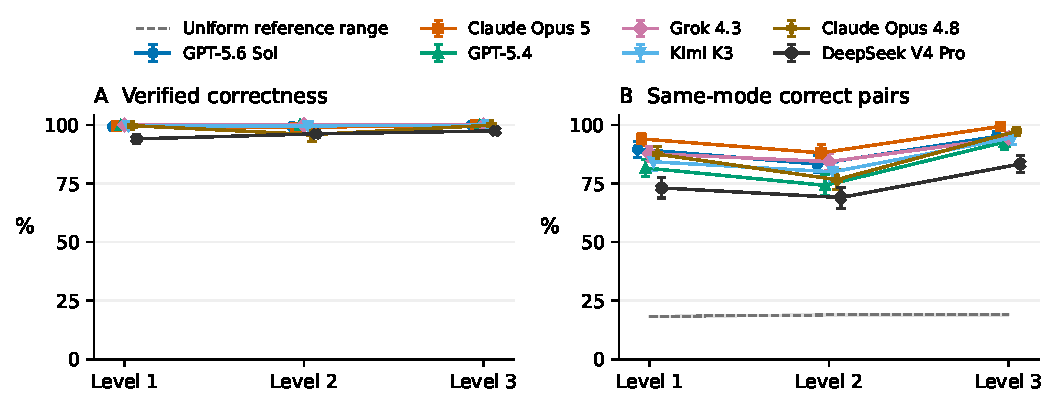
\includegraphics[width=\linewidth]{figures/frontier_comparison_20260911_graph.pdf}
  \caption{\textbf{Hosted \texttt{Graph} answers are usually correct but concentrated relative to uniform sampling.}
  Panel A shows strict per-response accuracy; panel B shows the fraction of
  correct pairs sharing a solution mode, pooling pairs across prompts. Colors
  and markers identify seven deployments, each with the same 128 prompts per
  level and eight stateless responses per prompt. Error bars are pointwise
  95\% intervals from resampling whole prompts. The gray band spans the
  deployments' uniform-correct-mode references, weighted by
  correct-pair counts; the dashed line is their mean. Level labels imply
  neither equal nor monotone difficulty across deployments.}
  \label{fig:hosted-graph-comparison}
\end{figure}

\subsection{A separate Python prompt sensitivity test}
\label{app:hosted-python-prompt}
After the original Opus 5 Python refusals, synthetic tasks were used to select
a direct arithmetic-expression formulation with no system message. We then
collected eight independent draws for every original Python test task: all
384 prompts across three levels, with unchanged adaptive thinking, medium
effort, 8,192 output tokens, allowed operators, public inputs and frozen graders.
The revised user instruction asks for a one-line boxed Python lambda returning
any proper divisor for each listed input. It does not prescribe a preferred divisor.
Both task wording and system-message presence change; collection time also differs.
This exploratory follow-up therefore supports a practical prompt repair without
isolating its cause. Original refusals and all three residual refusals are retained.
The original-protocol appendix tables retain all original Python responses;
the main display uses this complete revised condition with an explicit caption note.

\begin{table}[!htbp]
  \centering
  \caption{\textbf{Opus 5 Python: original versus plain task wording.}
  Each row has 1,024 responses. R counts native refusals; A is per-response accuracy (\%),
  D is \texttt{distinct@8}, and C is correct-pair collision (\%).
  Strict and normalized results use the same frozen grader and typography rule.
  Original Level-2/3 collision is undefined because no prompt has two correct draws.}
  \small
  \setlength{\tabcolsep}{4pt}
  \begin{tabular}{@{}llrrrrrrr@{}}
    \toprule
    & & & \multicolumn{3}{c}{Strict} & \multicolumn{3}{c}{Normalized} \\
    Condition & L & R & A & D & C & A & D & C \\
    \midrule
    Original & 1 & 409 & 38.1 & 0.91 & 93.0 & 60.0 & 1.12 & 90.4 \\
     & 2 & 1021 & 0.3 & 0.02 & -- & 0.3 & 0.02 & -- \\
     & 3 & 1024 & 0.0 & 0.00 & -- & 0.0 & 0.00 & -- \\
    \midrule
    Plain user, no system & 1 & 0 & 74.9 & 1.42 & 80.2 & 100.0 & 1.49 & 79.9 \\
     & 2 & 0 & 71.8 & 1.31 & 84.7 & 100.0 & 1.38 & 85.7 \\
     & 3 & 3 & 76.2 & 1.38 & 82.7 & 99.7 & 1.41 & 84.1 \\
    \bottomrule
  \end{tabular}
\end{table}

The new condition has no API failures or token-limit truncations. Strict grading
accepts 2,282 responses; the frozen rule rescues 787 more
by converting escaped percent signs (\verb|\%|) to Python modulo (\verb|%|).
Thus every non-refused answer passes after this formatting-only correction.
Normalized collision is 79.9/85.7/84.1\%, versus conditional uniform references
of 1.43/1.15/1.15\%. The residual three refusals occur on two prompts whose
other identical requests are accepted. No retry-until-accepted selection is used.

The paired analysis resamples whole eight-draw prompt groups across conditions
(20,000 replicates). Normalized accuracy gains at Levels 1/2/3 are
40.0 [34.7, 45.5], 99.7 [99.3, 100.0], and 99.7 [99.2, 100.0] percentage points
(pointwise 95\% intervals). Output draws themselves are independent, and the
different correct-pair populations preclude interpreting a raw collision
difference as a matched-population prompt effect.

The saved sensitivity record binds the original and revised native receipts,
request payloads, strict regrade audit and frozen normalization outputs.

\paragraph{Separate first-valid retry diagnostic.}
After completing the fixed 3,072-response revised-wording cohort, a separate
condition retries only its three remaining refused slots, retaining the
first verified-valid response. All three succeed on their first additional
request, and all reproduce a mode already seen for that prompt. This uses
3,075 requests to select 3,072 valid responses; its 100\% accepted-set
accuracy follows from selection and is not unconditional model accuracy.
The selected set's \texttt{distinct@8} is unchanged at 1.492, 1.375, 1.414 at
Levels 1--3. Level-3 correct-pair collision changes from 84.0909\% to 84.1518\%;
the other levels are unchanged. All initial and retry responses remain
preserved. The main figure continues to use the complete fixed eight-draw
condition, including its three refusals; these selected-validity results
are only a separate diagnostic with variable request effort.


\subsection{Requested-temperature sensitivity}
\label{app:hosted-temperature}
Grok 4.3 and Kimi K3 each receive requested temperatures $T=1.0$ and
$T=1.5$ on the same 120 tasks: eight prompts in each of five domains and
three levels. Eight responses from separate requests per prompt give 960
responses per deployment--temperature condition and 3,840 in total.
Within each deployment, the two conditions share all non-temperature
request settings and run concurrently. Accuracy and mode counts include
all responses, including verification failures and truncated outputs.

The providers accept both requested temperature settings, but their responses
do not report effective sampling temperatures. DeepSeek is outside this
comparison because its thinking-mode interface ignores the temperature setting.
The results concern these requested settings on this 120-task subset and
do not establish a general temperature response for all hosted deployments.

Each level summary averages five domains equally; All averages the 15
domain--level cells equally. Collision pools correct pairs within each cell,
so tasks with more correct responses receive more weight. Eligible tasks
and pair weights can differ between temperatures; the contrast does not
hold accuracy or the correct-pair population fixed. An undefined cell makes
the corresponding average undefined. Pointwise 95\% intervals use 20,000
paired whole-prompt bootstrap resamples, stratified by domain and level.
Each resampled prompt includes all eight responses. Prompts are paired
across conditions; output draws are not. Intervals have no multiplicity adjustment.

\paragraph{Observed sensitivity.}
For Grok, the observed diversity change is +0.050 [$-$0.058, +0.158] modes, and the collision change is $-$0.78 [$-$3.86, +2.12] percentage points. Both intervals include zero, so neither shows a clear diversity gain.
The per-response accuracy change is $-$2.29 [$-$3.85, $-$0.94] percentage points. These results do not establish invariance to temperature in general.

At $T=1.5$, 696 of Kimi's 960 outputs reach the token limit,
compared with 0 at $T=1.0$. Strict accuracy falls from 96.56\% to 21.25\%, while raw diversity falls from 1.933 to 0.983 modes.
The large increase in truncation accompanies losses in accuracy and distinct modes.
These results do not isolate correct-output concentration at matched accuracy.
The five-domain collision mean is undefined at
$T=1.5$ because some cells have no eligible correct pairs. Neither model
has provider-declared refusals in this experiment.

$\dagger$ marks a defined contrast whose interval is omitted because some
bootstrap resamples have undefined cells. Five-domain averages require all
five cell estimates; conditioning on only the estimable resamples would
change the uncertainty calculation.

\begin{table}[!htbp]
  \centering
  \setlength{\parfillskip}{0pt plus .20\linewidth}
  \caption{\textbf{Higher requested temperature yields no clear Grok diversity gain and much lower Kimi accuracy.} Strict executable grades compare $T=1.5$ with $T=1.0$.
  Each condition contains eight responses on each of 120 tasks.
  Level summaries average five domains equally; All averages 15 domain--level cells.
  A is per-response accuracy (\%); D is mean \texttt{distinct@8};
  C is correct-pair collision (\%), pooling pairs within each cell.
  Differences subtract $T=1.0$ from $T=1.5$: mode counts for D and percentage points for A/C.
  Brackets give pointwise 95\% intervals from paired whole-prompt bootstrap resampling.
  $\dagger$ marks an omitted interval when some resamples have undefined cells;
  -- denotes an undefined estimate or omitted interval.}
  \small
  \setlength{\tabcolsep}{5pt}
  \begin{tabular}{@{}llrrrr@{}}
    \toprule
    Deployment & Level & Metric & $T=1.0$ & $T=1.5$ & Difference [95\% interval] \\
    \midrule
    Grok 4.3 & 1 & A & 98.12 & 95.62 & $-$2.50 [$-$4.06, $-$0.94] \\
     &  & D & 1.900 & 2.000 & +0.100 [$-$0.100, +0.300] \\
     &  & C & 72.89 & 73.16 & +0.27 [$-$6.31, +6.37] \\
     & 2 & A & 99.06 & 99.38 & +0.31 [$-$0.94, +1.56] \\
     &  & D & 1.425 & 1.425 & +0.000 [$-$0.175, +0.200] \\
     &  & C & 86.61 & 85.20 & $-$1.41 [$-$6.26, +3.30] \\
     & 3 & A & 98.75 & 94.06 & $-$4.69 [$-$9.06, $-$0.94] \\
     &  & D & 1.500 & 1.550 & +0.050 [$-$0.125, +0.225] \\
     &  & C & 84.04 & 82.85 & $-$1.20 [$-$5.48, +2.79] \\
     & All & A & 98.65 & 96.35 & $-$2.29 [$-$3.85, $-$0.94] \\
     &  & D & 1.608 & 1.658 & +0.050 [$-$0.058, +0.158] \\
     &  & C & 81.18 & 80.40 & $-$0.78 [$-$3.86, +2.12] \\
    \midrule
    Kimi K3 & 1 & A & 92.50 & 22.50 & $-$70.00 [$-$75.62, $-$63.75] \\
     &  & D & 2.200 & 1.075 & $-$1.125 [$-$1.475, $-$0.775] \\
     &  & C & 66.23 & 53.12 & $-$13.11 [--]$^\dagger$ \\
     & 2 & A & 98.12 & 20.31 & $-$77.81 [$-$82.50, $-$72.81] \\
     &  & D & 1.850 & 0.900 & $-$0.950 [$-$1.300, $-$0.625] \\
     &  & C & 72.18 & 66.55 & $-$5.63 [--]$^\dagger$ \\
     & 3 & A & 99.06 & 20.94 & $-$78.12 [$-$83.75, $-$72.81] \\
     &  & D & 1.750 & 0.975 & $-$0.775 [$-$1.025, $-$0.525] \\
     &  & C & 78.33 & -- & -- \\
     & All & A & 96.56 & 21.25 & $-$75.31 [$-$78.44, $-$72.19] \\
     &  & D & 1.933 & 0.983 & $-$0.950 [$-$1.133, $-$0.767] \\
     &  & C & 72.25 & -- & -- \\
    \bottomrule
  \end{tabular}
\end{table}

\begin{table}[!htbp]
  \centering
  \setlength{\parfillskip}{0pt plus .20\linewidth}
  \caption{\textbf{Formatting normalization leaves the temperature sensitivity largely unchanged.} Only rows differing from strict grading appear; all other rows are identical.
  Each condition contains eight responses on each of 120 tasks.
  Level summaries average five domains equally; All averages 15 domain--level cells.
  A is per-response accuracy (\%); D is mean \texttt{distinct@8};
  C is correct-pair collision (\%), pooling pairs within each cell.
  Differences subtract $T=1.0$ from $T=1.5$: mode counts for D and percentage points for A/C.
  Brackets give pointwise 95\% intervals from paired whole-prompt bootstrap resampling.
  $\dagger$ marks an omitted interval when some resamples have undefined cells;
  -- denotes an undefined estimate or omitted interval.}
  \small
  \setlength{\tabcolsep}{5pt}
  \begin{tabular}{@{}llrrrr@{}}
    \toprule
    Deployment & Level & Metric & $T=1.0$ & $T=1.5$ & Difference [95\% interval] \\
    \midrule
    Kimi K3 & 1 & A & 92.50 & 22.81 & $-$69.69 [$-$75.31, $-$63.44] \\
     & 1 & C & 66.23 & 53.61 & $-$12.62 [--]$^\dagger$ \\
     & 3 & A & 99.38 & 20.94 & $-$78.44 [$-$84.06, $-$73.12] \\
     & 3 & C & 78.18 & -- & -- \\
     & All & A & 96.67 & 21.35 & $-$75.31 [$-$78.44, $-$72.19] \\
     & All & C & 72.20 & -- & -- \\
    \bottomrule
  \end{tabular}
\end{table}

Across the hosted comparisons, \texttt{Countdown} has no uniform reference because its
total support is not certified, so uniform-reference comparisons use the other
four domains. Cross-level differences
also reflect different task populations and do not establish a common ordering
of model difficulty. These inference-only results do not identify a training
or parameter-scale cause of concentration.


\subsection{GPT-5.6 Sol: temperature, pass@8 and verified modes}
\label{app:gpt56-temperature}
Figure~\ref{fig:gpt56-temperature-curve} plots empirical \texttt{pass@8}
against \texttt{distinct@8} for $T\in\{0.0,0.5,1.0,1.5,2.0\}$, with reasoning
\texttt{none}. Each condition uses the same 480 held-out prompts
(32 per domain--level cell), with eight stateless responses per prompt:
3,840 responses per temperature and 19,200 in total. A prompt contributes one
to \texttt{pass@8} if at least one of its eight answers is verified correct,
and contributes its number of distinct correct canonical keys to \texttt{distinct@8}.
Both metrics average over all prompts, including those with no correct answer.
The empirical \texttt{pass@8} uses the observed eight-response groups;
$1-(1-p)^8$ applied to pooled accuracy would ignore differences among prompts.
Raw \texttt{distinct@8} depends on both success and variation among correct
solution modes, so its changes need not track \texttt{pass@8}.

Prompts are selected independently of model outputs within each
domain--level cell. The evaluation comprises 120-prompt and 360-prompt
subsets collected at different times. Temperatures are interleaved for the
360-prompt subset; zero and nonzero temperatures are collected separately
for the 120-prompt subset. Service changes can therefore confound temperature
contrasts, and prompt composition can affect comparisons between subsets.

Requests use the same prompt wording, verifiers and sampling controls
except temperature, with an 8,192-token output cap. Returned metadata
identifies \texttt{gpt-5.6-sol-2026-07-09}, reasoning \texttt{none},
$\texttt{top\_p}=0.98$ and the requested temperature in every condition.
The exposed settings do not establish unchanged internal service behavior
or independent provider randomness. A zero-temperature request does not
establish deterministic outputs. The deployment rejects non-default
temperatures with medium reasoning and rejects temperature 2.5; this
sweep therefore does not test temperature robustness under medium reasoning.

Strict grading applies the executable validators directly. Normalized
grading uses the typography rules in App.~\ref{app:hosted-concentration}
before the same validators, preserving strict successes and their mode keys.

Each level averages five domains equally; All averages all 15 cells.
Pointwise 95\% intervals use 20,000 paired whole-prompt bootstrap
resamples stratified by domain and level, keeping all eight responses
together and matching prompts across temperatures. Individual model
responses are not paired across conditions.
There is no multiplicity adjustment. A zero-width empirical interval
reflects constant observed groups, not certain success on unseen prompts.

\begin{table}[!htbp]
\centering
\setlength{\parfillskip}{0pt plus .20\linewidth}
\caption{\textbf{Nonzero temperatures improve eight-draw coverage in this sweep.}
P is solved prompts (\%, \texttt{pass@8}); D is \texttt{distinct@8};
A is per-response accuracy (\%). G is the grading: S strict,
N formatting-normalized. Each temperature uses the same 480 prompts
(32 per domain--level cell), eight responses each, and reasoning \texttt{none}.
Level rows average five domains equally; All averages all 15 cells.
Brackets give pointwise 95\% whole-prompt bootstrap intervals.}
\label{tab:gpt56-temperature}
\small
\setlength{\tabcolsep}{4pt}
\begin{tabular}{@{}lllrrr@{}}
\toprule
$T$ & Level & G & P [95\% interval] & D [95\% interval] & A [95\% interval] \\
\midrule
0.0 & 1 & S & 55.0 [48.8, 61.3] & 0.569 [0.500, 0.637] & 53.9 [47.7, 60.1] \\
 & 2 &  & 45.0 [39.4, 50.6] & 0.456 [0.400, 0.512] & 39.5 [34.4, 44.7] \\
 & 3 &  & 49.4 [42.5, 56.2] & 0.519 [0.444, 0.594] & 44.5 [38.3, 50.9] \\
 & All &  & 49.8 [46.2, 53.3] & 0.515 [0.475, 0.554] & 46.0 [42.6, 49.4] \\
0.5 & 1 & S & 70.6 [64.4, 76.9] & 0.956 [0.850, 1.069] & 57.5 [51.9, 63.0] \\
 & 2 &  & 50.0 [44.4, 55.6] & 0.525 [0.463, 0.594] & 38.6 [33.9, 43.4] \\
 & 3 &  & 54.4 [48.1, 60.6] & 0.581 [0.506, 0.662] & 43.0 [37.1, 48.9] \\
 & All &  & 58.3 [54.8, 61.9] & 0.688 [0.640, 0.738] & 46.4 [43.3, 49.5] \\
1.0 & 1 & S & 75.6 [69.4, 81.2] & 1.181 [1.050, 1.312] & 57.3 [52.0, 62.7] \\
 & 2 &  & 51.9 [45.6, 58.1] & 0.581 [0.506, 0.662] & 37.6 [33.2, 42.0] \\
 & 3 &  & 60.6 [54.4, 66.9] & 0.713 [0.625, 0.806] & 42.7 [37.3, 48.1] \\
 & All &  & 62.7 [59.2, 66.2] & 0.825 [0.767, 0.885] & 45.9 [42.9, 48.8] \\
1.5 & 1 & S & 80.6 [75.0, 86.2] & 1.413 [1.269, 1.556] & 56.6 [51.7, 61.4] \\
 & 2 &  & 58.1 [51.9, 64.4] & 0.650 [0.569, 0.738] & 38.4 [34.3, 42.7] \\
 & 3 &  & 65.6 [59.4, 71.2] & 0.838 [0.731, 0.956] & 43.0 [38.0, 48.2] \\
 & All &  & 68.1 [64.8, 71.5] & 0.967 [0.900, 1.035] & 46.0 [43.3, 48.8] \\
2.0 & 1 & S & 83.8 [78.1, 88.8] & 1.519 [1.375, 1.663] & 59.7 [54.8, 64.5] \\
 & 2 &  & 54.4 [48.1, 60.6] & 0.600 [0.525, 0.675] & 35.3 [31.4, 39.3] \\
 & 3 &  & 61.9 [56.2, 67.5] & 0.819 [0.719, 0.925] & 40.5 [35.8, 45.5] \\
 & All &  & 66.7 [63.3, 70.0] & 0.979 [0.915, 1.044] & 45.2 [42.6, 47.8] \\
\midrule
0.0 & 1 & N & 70.6 [65.0, 76.2] & 0.725 [0.662, 0.788] & 70.5 [64.5, 76.2] \\
 & 2 &  & 60.6 [55.0, 66.2] & 0.613 [0.556, 0.669] & 54.5 [49.0, 59.9] \\
 & 3 &  & 65.6 [59.4, 71.9] & 0.681 [0.606, 0.756] & 61.4 [55.2, 67.6] \\
 & All &  & 65.6 [62.3, 69.0] & 0.673 [0.635, 0.710] & 62.1 [58.8, 65.5] \\
0.5 & 1 & N & 76.9 [71.2, 82.5] & 1.038 [0.931, 1.150] & 71.7 [66.4, 77.0] \\
 & 2 &  & 68.1 [62.5, 73.8] & 0.706 [0.644, 0.769] & 53.7 [48.8, 58.6] \\
 & 3 &  & 71.9 [65.6, 77.5] & 0.775 [0.700, 0.850] & 58.1 [52.3, 63.9] \\
 & All &  & 72.3 [69.2, 75.4] & 0.840 [0.792, 0.890] & 61.2 [58.2, 64.3] \\
1.0 & 1 & N & 79.4 [73.8, 84.4] & 1.238 [1.106, 1.369] & 70.4 [65.2, 75.5] \\
 & 2 &  & 69.4 [63.7, 75.0] & 0.756 [0.681, 0.831] & 51.6 [47.1, 56.2] \\
 & 3 &  & 76.9 [71.2, 82.5] & 0.894 [0.806, 0.988] & 55.2 [49.8, 60.7] \\
 & All &  & 75.2 [72.1, 78.3] & 0.963 [0.904, 1.021] & 59.1 [56.2, 62.0] \\
1.5 & 1 & N & 82.5 [77.5, 87.5] & 1.494 [1.344, 1.644] & 68.5 [63.7, 73.3] \\
 & 2 &  & 75.0 [69.4, 80.6] & 0.844 [0.762, 0.931] & 49.8 [45.5, 54.3] \\
 & 3 &  & 81.9 [76.2, 87.5] & 1.038 [0.931, 1.156] & 54.7 [49.6, 59.8] \\
 & All &  & 79.8 [76.7, 82.9] & 1.125 [1.056, 1.196] & 57.7 [54.9, 60.5] \\
2.0 & 1 & N & 85.0 [80.0, 90.0] & 1.606 [1.456, 1.762] & 69.6 [64.8, 74.3] \\
 & 2 &  & 72.5 [66.9, 78.1] & 0.800 [0.731, 0.869] & 45.7 [41.7, 49.8] \\
 & 3 &  & 80.6 [75.0, 86.2] & 1.031 [0.931, 1.137] & 52.5 [47.7, 57.5] \\
 & All &  & 79.4 [76.2, 82.5] & 1.146 [1.079, 1.212] & 55.9 [53.3, 58.6] \\
\bottomrule
\end{tabular}
\end{table}

\paragraph{Coverage and sampled solution modes.}
At $T=0.0$ and $T=2.0$, normalized \texttt{pass@8} is 65.62\% and 79.38\%, respectively,
while \texttt{distinct@8} is 0.673 and 1.146.
Across these five measured temperatures, the highest observed aggregate
\texttt{pass@8} occurs at $T=1.5$ and the highest \texttt{distinct@8}
occurs at $T=2.0$. These five temperatures do not establish
a population optimum or a continuous Pareto boundary, and level-specific curves differ.

Per-response accuracy changes from 62.11\% to 55.94\% between the endpoints.
That diagnostic is distinct from \texttt{pass@8}: success within eight
draws and the reliability of an individual draw need not change together as temperature varies.

The paired $T=2.0$ minus $T=0.0$ contrast is 13.8 [10.8, 16.7] \texttt{pass@8} percentage points and 0.473 [0.417, 0.529] distinct correct modes, with pointwise 95\% intervals.

\paragraph{Response outcomes.}
At every temperature, none of the 3,840 outputs is token-limited or a provider-declared refusal.
Unsuccessful answers remain in the eight-response groups.

\paragraph{Sensitivity across prompt subsets.}
We compare the same temperature contrast within each prompt subset.
The subsets differ in prompts and collection periods, so differences
between them do not isolate a causal effect of time. Brackets are
pointwise 95\% intervals.

Across all 480 prompts, the paired $T=2$ minus $T=1.5$ contrast is $-$0.4 [$-$2.5, 1.7] \texttt{pass@8} percentage points and 0.021 [$-$0.029, 0.071] distinct modes.
In the 120-prompt subset it is $-$1.7 [$-$5.0, 0.8] points and $-$0.008 [$-$0.083, 0.067] modes, and in the 360-prompt subset it is 0.0 [$-$2.8, 2.8] points and 0.031 [$-$0.033, 0.094] modes.

\subsection{Native provider outcomes and undefined concentration}
\label{app:hosted-provider-outcomes}
Provider metadata distinguish refusal and filtering from executable correctness.
A refusal does not establish that the underlying model cannot solve the task.
Classification uses native stop reasons, refusal fields and filter metadata;
it does not detect refusals expressed only in ordinary answer text.
An empty visible answer is a failed draw, including when the response contains
reasoning output. Empty-answer and refusal counts therefore need not agree.

Correct-pair collision requires at least two correct draws on one prompt.
It is undefined otherwise, as is a five-domain mean containing any undefined
domain. Dashes denote these undefined values. Accuracy and distinct-mode
counts include all responses, with zero correct modes on unsuccessful prompts.

Native completion states over the 15,360 original-instruction responses per deployment are:

\begin{itemize}\setlength{\itemsep}{0pt}
\item GPT-5.6 Sol --- completed: 15,360
\item Claude Opus 5 --- end\_turn: 12,838, refusal: 2,522
\item GPT-5.4 --- completed: 15,355, incomplete: 5
\item Grok 4.3 --- stop: 15,360
\item Kimi K3 --- length: 15, stop: 15,345
\item Claude Opus 4.8 --- end\_turn: 15,355, max\_tokens: 5
\item DeepSeek V4 Pro --- length: 632, stop: 14,728
\end{itemize}

Claude Opus 5 returns provider-declared refusals for 409, 1,021 and 1,024 of the 1,024 \texttt{Python} requests at Levels 1, 2 and 3, respectively.
The provider assigns them the refusal category cyber (2,454). These labels describe service behavior on factor-selection tasks;
they do not measure concentration among correct \texttt{Python} outputs.

\begin{table}[!htbp]
  \centering
  \caption{\textbf{Provider-declared refusals occur only for Opus 5 in this cohort.} Each original-instruction cell contains 128 prompts with eight responses each (1,024 responses). R counts native refusal signals, F native content filters, and E responses without visible answer text, including reasoning-only outputs. Counters can overlap and are separate from executable grades. Only cells with a nonzero counter appear; the other 83 of 105 cells have $R=F=E=0$, including all cells for GPT-5.6 Sol, Grok 4.3 and Kimi K3. Zero R does not exclude refusals expressed only in answer text.}
  \label{tab:hosted-provider-outcomes}
  \small
  \setlength{\tabcolsep}{5pt}
  \begin{tabular}{@{}llrrrr@{}}
    \toprule
    \textbf{Deployment} & \textbf{L} & \textbf{Domain} &
      \textbf{R} & \textbf{F} & \textbf{E} \\
    \midrule
    Claude Opus 5 & 1 & \texttt{Python} & 409 & 0 & 409 \\
     & 2 & \texttt{Python} & 1021 & 0 & 1021 \\
     & 2 & \texttt{MathIR} & 35 & 0 & 35 \\
     & 3 & \texttt{Python} & 1024 & 0 & 1024 \\
     & 3 & \texttt{MathIR} & 33 & 0 & 32 \\
    GPT-5.4 & 1 & \texttt{PantryPlan} & 0 & 0 & 1 \\
     & 2 & \texttt{Countdown} & 0 & 0 & 1 \\
     & 3 & \texttt{Countdown} & 0 & 0 & 1 \\
     & 3 & \texttt{PantryPlan} & 0 & 0 & 2 \\
    Claude Opus 4.8 & 3 & \texttt{Countdown} & 0 & 0 & 3 \\
     & 3 & \texttt{PantryPlan} & 0 & 0 & 1 \\
    DeepSeek V4 Pro & 1 & \texttt{Graph} & 0 & 0 & 59 \\
     & 1 & \texttt{MathIR} & 0 & 0 & 4 \\
     & 1 & \texttt{PantryPlan} & 0 & 0 & 13 \\
     & 2 & \texttt{Graph} & 0 & 0 & 38 \\
     & 2 & \texttt{Countdown} & 0 & 0 & 1 \\
     & 2 & \texttt{MathIR} & 0 & 0 & 59 \\
     & 2 & \texttt{PantryPlan} & 0 & 0 & 80 \\
     & 3 & \texttt{Graph} & 0 & 0 & 24 \\
     & 3 & \texttt{Countdown} & 0 & 0 & 7 \\
     & 3 & \texttt{MathIR} & 0 & 0 & 100 \\
     & 3 & \texttt{PantryPlan} & 0 & 0 & 246 \\
    \bottomrule
  \end{tabular}
\end{table}



\begin{table}[!htbp]
  \centering
  \caption{\textbf{Hosted deployments average fewer than three distinct correct modes per prompt.}
  Each row averages five domains equally under strict grading and original
  instructions, with 128 prompts per domain and eight responses per prompt.
  M/P are \texttt{mean@8}/\texttt{pass@8} (\%); D averages distinct correct
  solution modes, including zeros. C is correct-pair collision (\%), pooling
  pairs within each domain before averaging domains. Pointwise 95\% intervals
  use 2,000 whole-prompt bootstrap resamples within domains. A dash denotes
  an undefined domain collision and hence an undefined five-domain mean.
  Provider settings differ, so these are descriptive deployment comparisons.}
  \small
  \setlength{\tabcolsep}{3pt}
  \begin{tabular}{@{}lrrrrr@{}}
    \toprule
    Deployment & Level & M & P & D & C (95\% interval) \\
    \midrule
    GPT-5.6 Sol & 1 & 83.0 & 95.8 & 1.71 & 74.0 [71.9, 76.1] \\
GPT-5.6 Sol & 2 & 62.9 & 77.5 & 1.16 & 82.3 [80.3, 84.4] \\
GPT-5.6 Sol & 3 & 68.7 & 80.3 & 1.18 & 84.5 [82.8, 86.2] \\
\midrule
Claude Opus 5 & 1 & 85.3 & 94.5 & 1.32 & 86.3 [84.5, 88.0] \\
Claude Opus 5 & 2 & 76.6 & 80.2 & 1.16 & -- \\
Claude Opus 5 & 3 & 77.8 & 79.8 & 1.07 & -- \\
\midrule
GPT-5.4 & 1 & 93.7 & 98.1 & 2.09 & 67.2 [65.1, 69.3] \\
GPT-5.4 & 2 & 80.6 & 97.7 & 1.61 & 74.7 [72.4, 76.8] \\
GPT-5.4 & 3 & 83.3 & 97.8 & 1.57 & 78.8 [76.9, 80.7] \\
\midrule
Grok 4.3 & 1 & 98.3 & 99.5 & 1.97 & 72.4 [70.7, 74.0] \\
Grok 4.3 & 2 & 99.3 & 100.0 & 1.57 & 82.1 [80.6, 83.7] \\
Grok 4.3 & 3 & 98.8 & 100.0 & 1.55 & 83.0 [81.5, 84.6] \\
\midrule
Kimi K3 & 1 & 96.9 & 98.4 & 2.31 & 62.5 [60.6, 64.4] \\
Kimi K3 & 2 & 96.8 & 100.0 & 2.05 & 69.4 [67.6, 71.2] \\
Kimi K3 & 3 & 97.8 & 100.0 & 1.90 & 74.6 [73.1, 76.2] \\
\midrule
Claude Opus 4.8 & 1 & 96.4 & 98.8 & 1.64 & 78.4 [76.6, 80.3] \\
Claude Opus 4.8 & 2 & 98.5 & 100.0 & 1.67 & 77.2 [75.4, 79.1] \\
Claude Opus 4.8 & 3 & 98.9 & 99.8 & 1.51 & 83.4 [81.8, 84.9] \\
\midrule
DeepSeek V4 Pro & 1 & 96.4 & 98.4 & 2.01 & 71.0 [69.4, 72.7] \\
DeepSeek V4 Pro & 2 & 93.7 & 99.1 & 1.84 & 68.7 [67.0, 70.3] \\
DeepSeek V4 Pro & 3 & 91.0 & 99.7 & 1.62 & 78.8 [76.9, 80.9] \\
\bottomrule

  \end{tabular}
\end{table}

\begin{table}[!htbp]
  \centering
  \caption{\textbf{GPT-5.6 Sol: Strict executable grades.} Each cell has 128 prompts and 1,024 responses. M/P denote \texttt{mean@8}/\texttt{pass@8} (\%); D is \texttt{distinct@8}. C is correct-pair collision (\%) with pointwise 95\% prompt-bootstrap intervals. U is its conditional uniform reference (\%).}
  \small
  \setlength{\tabcolsep}{4pt}
  \begin{tabular}{@{}rlrrrrr@{}}
    \toprule
    Level & Domain & M & P & D & C (95\% interval) & U \\
    \midrule
    1 & Graph & 99.2 & 100.0 & 1.30 & 89.7 [86.3, 92.8] & 18.3 \\
    1 & Countdown & 86.1 & 98.4 & 1.77 & 71.2 [66.1, 75.9] & -- \\
    1 & Python & 40.4 & 90.6 & 1.11 & 81.8 [76.9, 87.2] & 0.8 \\
    1 & MathIR & 89.3 & 89.8 & 1.38 & 80.3 [75.4, 85.0] & 20.0 \\
    1 & PantryPlan & 100.0 & 100.0 & 3.00 & 46.9 [42.2, 51.5] & 6.5 \\
    \midrule
    2 & Graph & 99.3 & 100.0 & 1.48 & 83.3 [79.6, 87.0] & 18.9 \\
    2 & Countdown & 65.4 & 86.7 & 1.57 & 64.7 [59.0, 70.6] & -- \\
    2 & Python & 8.5 & 11.7 & 0.12 & 100.0 [100.0, 100.0] & 0.7 \\
    2 & MathIR & 86.2 & 93.0 & 0.93 & 100.0 [100.0, 100.0] & 20.0 \\
    2 & PantryPlan & 55.3 & 96.1 & 1.72 & 63.6 [56.8, 70.3] & 6.9 \\
    \midrule
    3 & Graph & 100.0 & 100.0 & 1.16 & 95.1 [92.4, 97.3] & 19.0 \\
    3 & Countdown & 71.2 & 89.8 & 1.38 & 76.4 [71.1, 81.8] & -- \\
    3 & Python & 9.4 & 14.1 & 0.14 & 100.0 [100.0, 100.0] & 0.9 \\
    3 & MathIR & 97.7 & 97.7 & 0.98 & 100.0 [100.0, 100.0] & 20.0 \\
    3 & PantryPlan & 65.3 & 100.0 & 2.22 & 51.0 [45.3, 57.3] & 6.8 \\
    \bottomrule
  \end{tabular}
\end{table}

\begin{table}[!htbp]
  \centering
  \caption{\textbf{Claude Opus 5: Strict executable grades.} Each cell has 128 prompts and 1,024 responses. M/P denote \texttt{mean@8}/\texttt{pass@8} (\%); D is \texttt{distinct@8}. C is correct-pair collision (\%) with pointwise 95\% prompt-bootstrap intervals. U is its conditional uniform reference (\%).}
  \small
  \setlength{\tabcolsep}{4pt}
  \begin{tabular}{@{}rlrrrrr@{}}
    \toprule
    Level & Domain & M & P & D & C (95\% interval) & U \\
    \midrule
    1 & Graph & 99.5 & 100.0 & 1.15 & 94.0 [91.3, 96.4] & 18.3 \\
    1 & Countdown & 100.0 & 100.0 & 1.59 & 78.8 [74.6, 83.0] & -- \\
    1 & Python & 38.1 & 81.2 & 0.91 & 93.0 [88.7, 96.6] & 0.7 \\
    1 & MathIR & 90.5 & 91.4 & 1.09 & 92.2 [88.8, 95.4] & 20.0 \\
    1 & PantryPlan & 98.4 & 100.0 & 1.86 & 73.5 [68.5, 78.2] & 6.5 \\
    \midrule
    2 & Graph & 98.9 & 100.0 & 1.32 & 88.1 [84.5, 91.6] & 18.9 \\
    2 & Countdown & 100.0 & 100.0 & 1.81 & 69.3 [65.2, 73.6] & -- \\
    2 & Python & 0.3 & 2.3 & 0.02 & -- & -- \\
    2 & MathIR & 89.1 & 98.4 & 1.06 & 96.5 [93.9, 98.6] & 20.0 \\
    2 & PantryPlan & 94.5 & 100.0 & 1.56 & 80.7 [76.0, 85.3] & 6.4 \\
    \midrule
    3 & Graph & 100.0 & 100.0 & 1.02 & 99.4 [98.3, 100.0] & 19.0 \\
    3 & Countdown & 99.9 & 100.0 & 1.66 & 76.2 [71.7, 80.7] & -- \\
    3 & Python & 0.0 & 0.0 & 0.00 & -- & -- \\
    3 & MathIR & 95.3 & 99.2 & 1.02 & 98.8 [97.5, 99.8] & 20.0 \\
    3 & PantryPlan & 93.6 & 100.0 & 1.63 & 78.8 [74.2, 83.4] & 6.5 \\
    \bottomrule
  \end{tabular}
\end{table}

\begin{table}[!htbp]
  \centering
  \caption{\textbf{GPT-5.4: Strict executable grades.} Each cell has 128 prompts and 1,024 responses. M/P denote \texttt{mean@8}/\texttt{pass@8} (\%); D is \texttt{distinct@8}. C is correct-pair collision (\%) with pointwise 95\% prompt-bootstrap intervals. U is its conditional uniform reference (\%).}
  \small
  \setlength{\tabcolsep}{4pt}
  \begin{tabular}{@{}rlrrrrr@{}}
    \toprule
    Level & Domain & M & P & D & C (95\% interval) & U \\
    \midrule
    1 & Graph & 99.8 & 100.0 & 1.57 & 81.6 [77.8, 85.4] & 18.3 \\
    1 & Countdown & 91.8 & 100.0 & 1.73 & 76.6 [71.2, 81.3] & -- \\
    1 & Python & 87.6 & 100.0 & 2.52 & 56.4 [51.3, 61.5] & 1.4 \\
    1 & MathIR & 89.3 & 90.6 & 1.45 & 78.6 [74.0, 83.4] & 20.0 \\
    1 & PantryPlan & 99.9 & 100.0 & 3.16 & 42.8 [38.4, 47.4] & 6.5 \\
    \midrule
    2 & Graph & 99.9 & 100.0 & 1.74 & 74.2 [69.8, 78.7] & 19.0 \\
    2 & Countdown & 91.1 & 100.0 & 1.98 & 63.0 [58.6, 67.5] & -- \\
    2 & Python & 47.9 & 96.1 & 1.47 & 72.9 [64.6, 80.2] & 1.0 \\
    2 & MathIR & 87.0 & 92.2 & 0.92 & 100.0 [100.0, 100.0] & 20.0 \\
    2 & PantryPlan & 77.0 & 100.0 & 1.93 & 63.2 [58.4, 68.6] & 6.8 \\
    \midrule
    3 & Graph & 99.8 & 100.0 & 1.23 & 92.7 [89.7, 95.4] & 19.0 \\
    3 & Countdown & 82.2 & 93.8 & 1.72 & 69.1 [64.4, 73.5] & -- \\
    3 & Python & 50.1 & 97.7 & 1.58 & 74.4 [68.6, 79.8] & 1.1 \\
    3 & MathIR & 97.7 & 97.7 & 0.98 & 100.0 [100.0, 100.0] & 20.0 \\
    3 & PantryPlan & 86.5 & 100.0 & 2.34 & 57.8 [52.8, 63.4] & 6.6 \\
    \bottomrule
  \end{tabular}
\end{table}

\begin{table}[!htbp]
  \centering
  \caption{\textbf{Grok 4.3: Strict executable grades.} Each cell has 128 prompts and 1,024 responses. M/P denote \texttt{mean@8}/\texttt{pass@8} (\%); D is \texttt{distinct@8}. C is correct-pair collision (\%) with pointwise 95\% prompt-bootstrap intervals. U is its conditional uniform reference (\%).}
  \small
  \setlength{\tabcolsep}{4pt}
  \begin{tabular}{@{}rlrrrrr@{}}
    \toprule
    Level & Domain & M & P & D & C (95\% interval) & U \\
    \midrule
    1 & Graph & 100.0 & 100.0 & 1.40 & 87.8 [84.2, 91.0] & 18.3 \\
    1 & Countdown & 99.9 & 100.0 & 2.05 & 64.8 [60.1, 69.5] & -- \\
    1 & Python & 99.8 & 100.0 & 1.41 & 88.0 [84.8, 91.0] & 1.4 \\
    1 & MathIR & 92.4 & 97.7 & 1.24 & 90.1 [86.9, 93.1] & 20.0 \\
    1 & PantryPlan & 99.4 & 100.0 & 3.77 & 31.4 [27.8, 35.1] & 6.5 \\
    \midrule
    2 & Graph & 99.9 & 100.0 & 1.52 & 84.3 [80.5, 88.0] & 19.0 \\
    2 & Countdown & 99.8 & 100.0 & 1.99 & 65.8 [61.8, 70.2] & -- \\
    2 & Python & 99.8 & 100.0 & 1.05 & 98.8 [97.8, 99.6] & 1.1 \\
    2 & MathIR & 97.5 & 100.0 & 1.12 & 94.9 [92.4, 97.2] & 20.0 \\
    2 & PantryPlan & 99.5 & 100.0 & 2.16 & 66.6 [61.2, 71.4] & 6.5 \\
    \midrule
    3 & Graph & 100.0 & 100.0 & 1.17 & 94.5 [92.0, 96.8] & 19.0 \\
    3 & Countdown & 99.9 & 100.0 & 1.98 & 66.3 [61.7, 71.0] & -- \\
    3 & Python & 99.9 & 100.0 & 1.04 & 98.6 [97.2, 99.6] & 1.2 \\
    3 & MathIR & 95.0 & 100.0 & 1.05 & 97.8 [95.9, 99.3] & 20.0 \\
    3 & PantryPlan & 99.2 & 100.0 & 2.52 & 58.0 [53.1, 63.5] & 6.5 \\
    \bottomrule
  \end{tabular}
\end{table}

\begin{table}[!htbp]
  \centering
  \caption{\textbf{Kimi K3: Strict executable grades.} Each cell has 128 prompts and 1,024 responses. M/P denote \texttt{mean@8}/\texttt{pass@8} (\%); D is \texttt{distinct@8}. C is correct-pair collision (\%) with pointwise 95\% prompt-bootstrap intervals. U is its conditional uniform reference (\%).}
  \small
  \setlength{\tabcolsep}{4pt}
  \begin{tabular}{@{}rlrrrrr@{}}
    \toprule
    Level & Domain & M & P & D & C (95\% interval) & U \\
    \midrule
    1 & Graph & 99.5 & 100.0 & 1.48 & 84.3 [80.4, 87.8] & 18.3 \\
    1 & Countdown & 99.1 & 100.0 & 1.91 & 68.4 [63.8, 73.3] & -- \\
    1 & Python & 97.9 & 100.0 & 2.52 & 57.7 [53.5, 61.9] & 1.4 \\
    1 & MathIR & 90.2 & 92.2 & 1.47 & 75.8 [70.7, 80.7] & 20.0 \\
    1 & PantryPlan & 97.5 & 100.0 & 4.18 & 26.2 [23.1, 29.2] & 6.5 \\
    \midrule
    2 & Graph & 99.6 & 100.0 & 1.62 & 80.0 [76.0, 84.1] & 19.0 \\
    2 & Countdown & 98.4 & 100.0 & 1.98 & 64.4 [59.9, 68.7] & -- \\
    2 & Python & 98.2 & 100.0 & 2.44 & 61.9 [57.6, 66.2] & 1.1 \\
    2 & MathIR & 94.3 & 100.0 & 1.02 & 99.8 [99.3, 100.0] & 20.0 \\
    2 & PantryPlan & 93.3 & 100.0 & 3.20 & 41.3 [36.6, 45.9] & 6.6 \\
    \midrule
    3 & Graph & 99.9 & 100.0 & 1.19 & 94.6 [91.8, 96.9] & 19.0 \\
    3 & Countdown & 97.5 & 100.0 & 1.84 & 70.6 [66.1, 74.8] & -- \\
    3 & Python & 98.0 & 100.0 & 2.34 & 64.7 [60.1, 69.0] & 1.2 \\
    3 & MathIR & 98.1 & 100.0 & 1.00 & 100.0 [100.0, 100.0] & 20.0 \\
    3 & PantryPlan & 95.6 & 100.0 & 3.13 & 43.4 [38.6, 48.3] & 6.5 \\
    \bottomrule
  \end{tabular}
\end{table}

\begin{table}[!htbp]
  \centering
  \caption{\textbf{Claude Opus 4.8: Strict executable grades.} Each cell has 128 prompts and 1,024 responses. M/P denote \texttt{mean@8}/\texttt{pass@8} (\%); D is \texttt{distinct@8}. C is correct-pair collision (\%) with pointwise 95\% prompt-bootstrap intervals. U is its conditional uniform reference (\%).}
  \small
  \setlength{\tabcolsep}{4pt}
  \begin{tabular}{@{}rlrrrrr@{}}
    \toprule
    Level & Domain & M & P & D & C (95\% interval) & U \\
    \midrule
    1 & Graph & 99.7 & 100.0 & 1.34 & 87.5 [83.9, 91.0] & 18.3 \\
    1 & Countdown & 95.6 & 99.2 & 1.78 & 69.8 [64.9, 74.5] & -- \\
    1 & Python & 98.0 & 100.0 & 1.40 & 85.7 [81.7, 89.4] & 1.4 \\
    1 & MathIR & 92.3 & 94.5 & 1.10 & 93.7 [91.1, 96.4] & 20.0 \\
    1 & PantryPlan & 96.6 & 100.0 & 2.59 & 55.3 [50.3, 60.1] & 6.5 \\
    \midrule
    2 & Graph & 95.9 & 100.0 & 1.66 & 76.6 [72.3, 81.1] & 18.8 \\
    2 & Countdown & 99.9 & 100.0 & 1.99 & 65.3 [60.9, 69.9] & -- \\
    2 & Python & 100.0 & 100.0 & 1.34 & 86.0 [82.3, 89.6] & 1.2 \\
    2 & MathIR & 97.0 & 100.0 & 1.24 & 90.1 [86.7, 93.4] & 20.0 \\
    2 & PantryPlan & 99.5 & 100.0 & 2.11 & 67.9 [62.8, 73.1] & 6.5 \\
    \midrule
    3 & Graph & 99.9 & 100.0 & 1.08 & 97.3 [95.5, 98.9] & 19.0 \\
    3 & Countdown & 97.9 & 99.2 & 1.80 & 72.5 [68.2, 76.6] & -- \\
    3 & Python & 98.9 & 100.0 & 1.32 & 86.4 [82.5, 90.1] & 1.2 \\
    3 & MathIR & 99.1 & 100.0 & 1.03 & 99.1 [98.1, 99.8] & 20.0 \\
    3 & PantryPlan & 98.5 & 100.0 & 2.33 & 61.6 [56.7, 66.6] & 6.5 \\
    \bottomrule
  \end{tabular}
\end{table}

\begin{table}[!htbp]
  \centering
  \caption{\textbf{DeepSeek V4 Pro: Strict executable grades.} Each cell has 128 prompts and 1,024 responses. M/P denote \texttt{mean@8}/\texttt{pass@8} (\%); D is \texttt{distinct@8}. C is correct-pair collision (\%) with pointwise 95\% prompt-bootstrap intervals. U is its conditional uniform reference (\%).}
  \small
  \setlength{\tabcolsep}{4pt}
  \begin{tabular}{@{}rlrrrrr@{}}
    \toprule
    Level & Domain & M & P & D & C (95\% interval) & U \\
    \midrule
    1 & Graph & 94.0 & 100.0 & 1.80 & 73.1 [68.8, 77.4] & 18.1 \\
    1 & Countdown & 100.0 & 100.0 & 2.02 & 65.8 [61.4, 70.3] & -- \\
    1 & Python & 99.3 & 100.0 & 1.41 & 88.8 [86.1, 91.4] & 1.4 \\
    1 & MathIR & 90.1 & 92.2 & 1.11 & 93.9 [91.2, 96.2] & 20.0 \\
    1 & PantryPlan & 98.5 & 100.0 & 3.73 & 33.5 [29.8, 37.2] & 6.5 \\
    \midrule
    2 & Graph & 96.2 & 100.0 & 1.97 & 69.0 [64.4, 73.5] & 19.1 \\
    2 & Countdown & 99.9 & 100.0 & 2.04 & 63.4 [59.2, 67.7] & -- \\
    2 & Python & 99.6 & 100.0 & 1.05 & 98.4 [97.1, 99.4] & 1.2 \\
    2 & MathIR & 85.4 & 95.3 & 1.82 & 51.7 [49.8, 53.9] & 20.0 \\
    2 & PantryPlan & 87.1 & 100.0 & 2.34 & 61.1 [56.0, 66.2] & 6.5 \\
    \midrule
    3 & Graph & 97.5 & 100.0 & 1.52 & 83.4 [79.6, 87.0] & 18.9 \\
    3 & Countdown & 99.2 & 100.0 & 1.98 & 67.5 [63.1, 72.2] & -- \\
    3 & Python & 99.6 & 100.0 & 1.08 & 97.8 [96.3, 99.0] & 1.2 \\
    3 & MathIR & 88.5 & 100.0 & 1.44 & 83.6 [79.2, 87.6] & 20.0 \\
    3 & PantryPlan & 70.3 & 98.4 & 2.08 & 61.9 [55.9, 68.2] & 6.5 \\
    \bottomrule
  \end{tabular}
\end{table}

\begin{table}[!htbp]
  \centering
  \caption{\textbf{Post hoc formatting diagnostic: the cells it changes.} Each cell has 128 prompts and 1,024 responses. M/P denote \texttt{mean@8}/\texttt{pass@8} (\%); D is \texttt{distinct@8}. C is correct-pair collision (\%) with pointwise 95\% prompt-bootstrap intervals. U is its conditional uniform reference (\%). Only cells whose normalized grade differs from its strict grade appear; every cell absent here is identical under both gradings. The normalizer rescued no response for Grok 4.3.}
  \scriptsize
  \setlength{\tabcolsep}{4pt}
  \begin{tabular}{@{}lrlrrrrr@{}}
    \toprule
    Deployment & Level & Domain & M & P & D & C (95\% interval) & U \\
    \midrule
    GPT-5.6 Sol & 1 & Countdown & 99.9 & 100.0 & 1.93 & 67.9 [63.3, 72.4] & -- \\
     & 1 & Python & 92.4 & 100.0 & 1.41 & 85.6 [82.3, 88.8] & 1.4 \\
     & 2 & Countdown & 98.5 & 100.0 & 1.99 & 63.9 [59.5, 68.4] & -- \\
     & 2 & Python & 60.7 & 99.2 & 1.12 & 94.8 [91.9, 97.2] & 1.1 \\
     & 2 & PantryPlan & 71.3 & 100.0 & 1.96 & 64.0 [58.1, 69.6] & 6.8 \\
     & 3 & Countdown & 99.0 & 100.0 & 1.70 & 75.7 [71.2, 80.1] & -- \\
     & 3 & Python & 56.5 & 98.4 & 1.09 & 94.3 [90.8, 97.2] & 1.0 \\
     & 3 & PantryPlan & 75.2 & 100.0 & 2.35 & 53.0 [47.3, 58.9] & 6.7 \\
    \addlinespace[2pt]
    Claude Opus 5 & 1 & Python & 60.0 & 94.5 & 1.12 & 90.4 [86.2, 94.3] & 0.9 \\
     & 2 & PantryPlan & 99.9 & 100.0 & 1.61 & 79.7 [75.0, 84.3] & 6.5 \\
     & 3 & Countdown & 100.0 & 100.0 & 1.66 & 76.1 [71.7, 80.7] & -- \\
     & 3 & PantryPlan & 99.4 & 100.0 & 1.70 & 77.3 [72.6, 82.0] & 6.5 \\
    \addlinespace[2pt]
    GPT-5.4 & 1 & Countdown & 99.7 & 100.0 & 1.80 & 73.6 [68.5, 78.3] & -- \\
     & 1 & Python & 98.7 & 100.0 & 2.57 & 56.8 [51.9, 61.6] & 1.4 \\
     & 2 & Countdown & 98.4 & 100.0 & 2.12 & 61.1 [57.0, 65.1] & -- \\
     & 2 & Python & 91.3 & 100.0 & 1.87 & 74.0 [69.4, 78.1] & 1.1 \\
     & 3 & Countdown & 99.0 & 100.0 & 1.96 & 68.4 [64.2, 72.7] & -- \\
     & 3 & Python & 91.6 & 100.0 & 1.91 & 72.6 [68.3, 77.1] & 1.2 \\
    \addlinespace[2pt]
    Kimi K3 & 1 & Countdown & 99.4 & 100.0 & 1.91 & 68.4 [63.9, 73.3] & -- \\
     & 1 & Python & 98.2 & 100.0 & 2.53 & 57.7 [53.5, 61.9] & 1.4 \\
     & 2 & Countdown & 98.7 & 100.0 & 1.98 & 64.5 [60.1, 68.9] & -- \\
     & 2 & Python & 98.3 & 100.0 & 2.44 & 61.9 [57.6, 66.2] & 1.1 \\
     & 2 & PantryPlan & 93.4 & 100.0 & 3.20 & 41.4 [36.7, 46.0] & 6.6 \\
     & 3 & Countdown & 98.1 & 100.0 & 1.84 & 70.3 [65.8, 74.5] & -- \\
     & 3 & Python & 98.5 & 100.0 & 2.34 & 64.9 [60.3, 69.2] & 1.2 \\
    \addlinespace[2pt]
    Claude Opus 4.8 & 1 & Python & 98.6 & 100.0 & 1.40 & 85.8 [81.8, 89.5] & 1.5 \\
     & 3 & PantryPlan & 98.7 & 100.0 & 2.33 & 61.7 [56.7, 66.6] & 6.5 \\
    \addlinespace[2pt]
    DeepSeek V4 Pro & 1 & Python & 99.4 & 100.0 & 1.41 & 88.8 [86.1, 91.4] & 1.4 \\
     & 2 & Python & 99.7 & 100.0 & 1.05 & 98.4 [97.1, 99.4] & 1.2 \\
     & 3 & Python & 99.7 & 100.0 & 1.08 & 97.8 [96.3, 99.0] & 1.2 \\
    \bottomrule
  \end{tabular}
\end{table}




% Generated by ops/build_paper_hosted_level_averages.py; do not edit.
\begin{table}[H]
  \centering
  \small
  \setlength{\tabcolsep}{4pt}
  \resizebox{\linewidth}{!}{%
  \begin{tabular}{lrrrrrrrrr}
    \toprule
    & \multicolumn{3}{c}{Level 1} & \multicolumn{3}{c}{Level 2} & \multicolumn{3}{c}{Level 3} \\
    \cmidrule(lr){2-4}\cmidrule(lr){5-7}\cmidrule(lr){8-10}
    Model & \texttt{pass@8} (\%) & \# modes & \pmd{} & \texttt{pass@8} (\%) & \# modes & \pmd{} & \texttt{pass@8} (\%) & \# modes & \pmd{} \\
    \midrule
    \raisebox{-0.15em}{
\includegraphics[width=1.05em,height=1.05em,keepaspectratio]{icons/openai.png}}\hspace{0.4em}GPT-5.6 Sol & 98.0 & 1.80 & .256 & 98.4 & 1.50 & .229\textsuperscript{\textdagger} & 99.2 & 1.45 & .183\textsuperscript{\textdagger} \\
    \raisebox{-0.15em}{
\includegraphics[width=1.05em,height=1.05em,keepaspectratio]{icons/claude.png}}\hspace{0.4em}Claude Opus 5 & 98.3\textsuperscript{\ensuremath{\ddagger}} & 1.43\textsuperscript{\ensuremath{\ddagger}} & .140 & 99.7\textsuperscript{\ensuremath{\ddagger}} & 1.44\textsuperscript{\ensuremath{\ddagger}} & .164\textsuperscript{\textdagger} & 99.8\textsuperscript{\ensuremath{\ddagger}} & 1.36\textsuperscript{\ensuremath{\ddagger}} & .121\textsuperscript{\textdagger} \\
    \raisebox{-0.15em}{
\includegraphics[width=1.05em,height=1.05em,keepaspectratio]{icons/openai.png}}\hspace{0.4em}GPT-5.4 & 98.1 & 2.11 & .338 & 98.4 & 1.72 & .247 & 99.5 & 1.68 & .224 \\
    \raisebox{-0.15em}{
\includegraphics[width=1.05em,height=1.05em,keepaspectratio]{icons/grok_official_docs_print.png}}\hspace{0.4em}Grok 4.3 & 99.5 & 1.97 & .275 & 100.0 & 1.57 & .179 & 100.0 & 1.55 & .171 \\
    \raisebox{-0.15em}{
\includegraphics[width=1.05em,height=1.05em,keepaspectratio]{icons/kimi.png}}\hspace{0.4em}Kimi K3 & 98.4 & 2.31 & .374 & 100.0 & 2.05 & .307 & 100.0 & 1.90 & .253 \\
    \raisebox{-0.15em}{
\includegraphics[width=1.05em,height=1.05em,keepaspectratio]{icons/claude.png}}\hspace{0.4em}Claude Opus 4.8 & 98.8 & 1.64 & .217 & 100.0 & 1.67 & .229 & 99.8 & 1.51 & .168 \\
    \raisebox{-0.15em}{
\includegraphics[width=1.05em,height=1.05em,keepaspectratio]{icons/deepseek.png}}\hspace{0.4em}DeepSeek V4 Pro & 98.4 & 2.01 & .289 & 99.1 & 1.84 & .319 & 99.7 & 1.62 & .232 \\
    \bottomrule
  \end{tabular}}
  \caption{\textbf{High prompt success coexists with few verified solution modes.}
  Each deployment requests medium reasoning effort, with 128 prompts per domain
  and level and eight responses per prompt. \texttt{pass@8} and \# modes use
  formatting-normalized grading and average the five domains equally:
  \texttt{pass@8} is empirical prompt success; \# modes is mean
  \texttt{distinct@8}, including zero for prompts without a verified response.
  \textsuperscript{\ensuremath{\ddagger}} marks the three Claude Opus 5 cells using
  revised \texttt{Python} wording without a system message (App.~\ref{app:hosted-python-prompt}).
  \pmd{} instead uses strict grading and the original wording throughout,
  averaging per-prompt diversity over prompts with at least two verified draws
  and then equally over reportable domains. These are the per-level columns of
  Table~\ref{tab:hosted-cohort-mode-diversity}, not its common-cell macro.
  \textsuperscript{\textdagger} marks four cells omitting \texttt{Python} because fewer
  than thirty prompts qualify: GPT-5.6 Sol has strict-formatting failures;
  Opus 5 has provider refusals. All entries are point estimates.
  Table~\ref{tab:hosted-level-averages-parity} gives normalized success and mode
  counts on the four domains with common wording.}
  \label{tab:hosted-level-averages-medium}
\end{table}


\begin{figure}[!htbp]
  \centering
  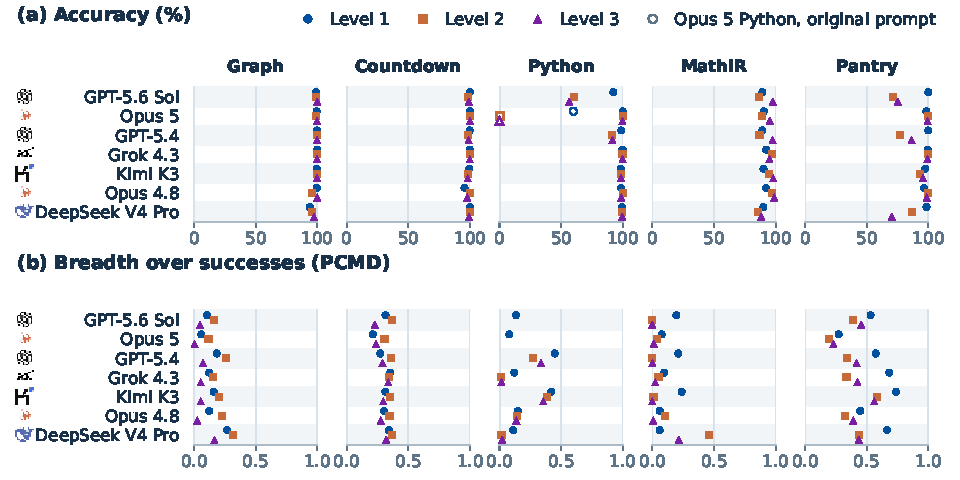
\includegraphics[width=\linewidth]{figures/hosted_verified_breadth.pdf}
  \caption{\textbf{Accurate hosted responses can still concentrate on few solution modes.}
  Columns show domains; colors and marker shapes distinguish Levels~1--3.
  Each deployment--domain--level cell uses 128 prompts and eight responses
  per prompt. Top: formatting-normalized response accuracy. Solid Opus~5
  \texttt{Python} marks use revised task wording without a system message; hollow marks
  show original wording. Bottom: promptwise \pmd{} under strict grading
  and original wording for every deployment, averaging over prompts with
  at least two verified draws. Cells with fewer than thirty eligible prompts
  are omitted. Thus the two rows use different grading and, for Opus~5
  \texttt{Python}, different prompt conditions. All marks are point estimates.
  Table~\ref{tab:hosted-level-averages-medium} gives per-level means;
  Table~\ref{tab:hosted-level-averages-parity} gives normalized success and
  mode counts on the four domains with common wording.}
  \label{fig:hosted-verified-breadth}
\end{figure}

% Generated by ops/build_paper_hosted_level_averages.py; do not edit.
\paragraph{Evaluation parity across deployments.}
One column of this cohort rests on wording the other deployments did not
answer: Claude Opus 5's Python cells in Fig.~\ref{fig:hosted-verified-breadth}
and Table~\ref{tab:hosted-level-averages-medium} use the revised condition of
App.~\ref{app:hosted-python-prompt}. Every other reading in this paper holds one
prompt across all seven deployments, including the \pmd{} column beside them,
Table~\ref{tab:hosted-cohort-mode-diversity} and the strict and normalized cell
tables above. Table~\ref{tab:hosted-level-averages-parity} therefore repeats the
comparison over Graph, Countdown, MathIR and Pantry alone, the four domains that share
one prompt. Claude Opus 5 averages
1.42/1.45/1.35 verified modes there at Levels 1--3,
against 1.43/1.44/1.36 over five domains with the
revised Python cell and 1.36/1.17/1.08
with the original one. It is the least varied deployment at every level under all
three readings, and the revised wording raises its Python breadth rather than
lowering it, so the substituted cell moves the five-domain reading away from
concentration rather than towards it. Which of the other six follows it varies
with Python in or out, as their per-domain disagreement in
Table~\ref{tab:hosted-cohort-mode-diversity} already reports; what survives every
reading is the level, not the order.
How far a Python wording change can carry this domain is itself measured, on
three of the other six: App.~\ref{app:sampling-budget-effects}
answers Python under two wordings at 16 prompts and
64 draws, and pooled \pmd{} moves by between
+.024 and +.131 across its
six deployment--level cells, leaving every one of them concentrated
under both wordings (highest \pmd{} .369,
$\neff$ 1.58). That bounds how far wording carries
this domain; it does not identify what this particular revision would do to a
deployment other than the one that answered it.

\begin{table}[H]
  \centering
  \small
  \setlength{\tabcolsep}{5pt}
  \begin{tabular}{lrrrrrr}
    \toprule
    & \multicolumn{2}{c}{Level 1} & \multicolumn{2}{c}{Level 2} & \multicolumn{2}{c}{Level 3} \\
    \cmidrule(lr){2-3}\cmidrule(lr){4-5}\cmidrule(lr){6-7}
    Model & \texttt{pass@8} (\%) & \# modes & \texttt{pass@8} (\%) & \# modes & \texttt{pass@8} (\%) & \# modes \\
    \midrule
    GPT-5.6 Sol & 97.5 & 1.90 & 98.2 & 1.59 & 99.4 & 1.54 \\
    Claude Opus 5 & 97.9 & 1.42 & 99.6 & 1.45 & 99.8 & 1.35 \\
    GPT-5.4 & 97.7 & 2.00 & 98.0 & 1.68 & 99.4 & 1.62 \\
    Grok 4.3 & 99.4 & 2.12 & 100.0 & 1.70 & 100.0 & 1.68 \\
    Kimi K3 & 98.0 & 2.26 & 100.0 & 1.95 & 100.0 & 1.79 \\
    Claude Opus 4.8 & 98.4 & 1.70 & 100.0 & 1.75 & 99.8 & 1.56 \\
    DeepSeek V4 Pro & 98.0 & 2.16 & 98.8 & 2.04 & 99.6 & 1.75 \\
    \bottomrule
  \end{tabular}
  \caption{\textbf{Hosted success and output diversity with Python excluded.}
  The same draws as Table~\ref{tab:hosted-level-averages-medium}, averaged over
  Graph, Countdown, MathIR and Pantry alone: the four domains every deployment answers
  under one prompt, 128 prompts each and eight responses per prompt. Reading this
  table beside that one shows what the revised Python condition of
  App.~\ref{app:hosted-python-prompt} carries, and what it does not.}
  \label{tab:hosted-level-averages-parity}
\end{table}


% Generated by ops/build_paper_gpt56sol_python_parity.py; do not edit.
\subsection{The revised \texttt{Python} wording on a second deployment}
\label{app:python-wording-second-deployment}

The original and revised \texttt{Python} conditions of App.~\ref{app:hosted-python-prompt}
are evaluated on GPT-5.6 Sol through \path{api.openai.com}. Each condition uses
the same 384 problems, with 128 prompts per level and eight responses per prompt,
medium reasoning effort and an 8,192-token output cap. The original condition
uses the benchmark request; the revised condition asks for a direct expression
without a system message. Public task inputs, allowed operators and the verifier
are unchanged, but wording and system-message presence change together.
Every response reports the model \texttt{gpt-5.6-sol}, but this build cannot be
shown to match the Azure deployment used for the hosted averages, so the two
are treated as separate populations.

\paragraph{Verified success and mode counts decrease under the revised condition.}
There are no provider-declared refusals among the
6,144 responses in this comparison.
The Azure GPT-5.6 Sol cohort also contains no provider-declared refusals;
its missing strict \texttt{Python} diversity entries reflect too few verified draws.
Under normalized grading, the revised condition lowers accuracy and mean
\texttt{distinct@8} at each level (Table~\ref{tab:gpt56sol-python-parity}).
Revised-minus-original differences use all 128 prompts per level, pairing
problems across conditions and resampling whole eight-response groups:
20,000 replicates give pointwise 95\% percentile intervals.
Accuracy differences are fractions of responses; mode-count differences are
modes per prompt:
accuracy $-.689$ $[-.745, -.631]$, $-.420$ $[-.467, -.374]$, $-.370$ $[-.418, -.320]$ at Levels 1--3;
\texttt{distinct@8} $-.945$ $[-1.078, -.820]$, $-.703$ $[-.812, -.594]$, $-.656$ $[-.766, -.547]$ respectively.
The revised normalized cells have
28, 26, 25
prompts with at least two verified responses, all below the 30-prompt
reporting threshold, so their success-conditional diversity and any diversity
contrast are omitted.

\paragraph{Formatting failures accompany the lower scores.}
The literal \LaTeX{} marker \verb|\text{| appears in
862 original-condition and
2,089 revised-condition responses
(28\% and 68\%).
The formatting normalizer does not remove this wrapper; none of these responses
verifies. Among responses without the marker, normalized success is
94.9\% and 59.3\%, respectively.
Absence of this marker does not guarantee parseability. Because the marker
depends on the response, these subsets are not matched comparisons and do not
bound a content or capability effect.

\paragraph{Prompt-interface sensitivity differs across deployments.}
The revised condition increases normalized success and verified mode counts
for Opus 5 (App.~\ref{app:hosted-python-prompt}) but decreases both for this
GPT-5.6 Sol deployment. This comparison does not isolate task wording from the
system message, establish that either task is generally easier, or identify
the effect on the remaining hosted deployments. The four-domain comparison in
Table~\ref{tab:hosted-level-averages-parity} holds the task prompts fixed across
all seven deployments by excluding \texttt{Python}.

\begin{table}[!htbp]
  \centering
  \caption{\textbf{The revised \texttt{Python} condition lowers normalized success and verified mode counts on GPT-5.6 Sol.}
  Both conditions use the same 128 problems per level and eight responses per
  prompt through \texttt{api.openai.com}, with medium reasoning effort and an
  8,192-token output cap. R counts provider-declared refusals; A is response
  accuracy (\%); D is mean \texttt{distinct@8} over all prompts.
  $1-C$ is pair-pooled diversity: the fraction of correct pairs with different
  solution modes, weighting each correct pair equally across prompts.
  Dashes mark cells with fewer than 30 prompts containing at least two
  verified draws. Strict grading uses the original output; normalized grading
  applies the same typography rules to both conditions. Entries are point
  estimates; paired uncertainty for accuracy and mode-count differences is
  given in the surrounding text.}
  \small
  \setlength{\tabcolsep}{4pt}
  \begin{tabular}{@{}llrrrrrrr@{}}
    \toprule
    & & & \multicolumn{3}{c}{Strict} & \multicolumn{3}{c}{Normalized} \\
    \cmidrule(lr){4-6}\cmidrule(lr){7-9}
    Wording & L & R & A & D & $1-C$ & A & D & $1-C$ \\
    \midrule
    Original & 1 & 0 & 37.0 & 1.02 & .106 & 89.8 & 1.36 & .114 \\
     & 2 & 0 & 10.4 & 0.14 & --- & 58.7 & 1.15 & .053 \\
     & 3 & 0 & 13.0 & 0.16 & --- & 56.3 & 1.13 & .048 \\
    \midrule
    Revised, no system & 1 & 0 & 18.7 & 0.27 & --- & 20.9 & 0.41 & --- \\
     & 2 & 0 & 13.4 & 0.26 & --- & 16.7 & 0.45 & --- \\
     & 3 & 0 & 15.5 & 0.25 & --- & 19.3 & 0.48 & --- \\
    \bottomrule
  \end{tabular}
  \label{tab:gpt56sol-python-parity}
\end{table}


% Generated by ops/build_paper_hosted_reasoning_off.py; do not edit.
\begin{table}[H]
  \centering
  \small
  \setlength{\tabcolsep}{5pt}
  \begin{tabular}{lrrrrrr}
    \toprule
    & \multicolumn{2}{c}{Level 1} & \multicolumn{2}{c}{Level 2} & \multicolumn{2}{c}{Level 3} \\
    \cmidrule(lr){2-3}\cmidrule(lr){4-5}\cmidrule(lr){6-7}
    Model & \texttt{pass@8} (\%) & \# modes & \texttt{pass@8} (\%) & \# modes & \texttt{pass@8} (\%) & \# modes \\
    \midrule
    \raisebox{-0.15em}{
\includegraphics[width=1.05em,height=1.05em,keepaspectratio]{icons/openai.png}}\hspace{0.4em}GPT-5.6 Sol & 82.5 & 1.31 & 66.9 & 0.76 & 76.2 & 0.88 \\
    \raisebox{-0.15em}{
\includegraphics[width=1.05em,height=1.05em,keepaspectratio]{icons/openai.png}}\hspace{0.4em}GPT-5.4 & 82.5 & 1.67 & 71.2 & 0.92 & 70.0 & 0.94 \\
    \raisebox{-0.15em}{
\includegraphics[width=1.05em,height=1.05em,keepaspectratio]{icons/grok_official_docs_print.png}}\hspace{0.4em}Grok 4.3 & 82.5 & 1.64 & 86.9 & 1.41 & 90.0 & 1.45 \\
    \raisebox{-0.15em}{
\includegraphics[width=1.05em,height=1.05em,keepaspectratio]{icons/kimi.png}}\hspace{0.4em}Kimi K3 & 92.5 & 1.91 & 92.5 & 1.37 & 95.6 & 1.59 \\
    \raisebox{-0.15em}{
\includegraphics[width=1.05em,height=1.05em,keepaspectratio]{icons/claude.png}}\hspace{0.4em}Claude Opus 4.8 & 91.2 & 1.46 & 100.0 & 1.62 & 100.0 & 1.51 \\
    \bottomrule
  \end{tabular}
  \caption{\textbf{Hosted success and output diversity with reasoning disabled.}
  Each level averages five domains equally: 32 prompts per domain and eight
  responses per prompt. \texttt{pass@8} is the fraction with any verified
  response; \# modes is mean \texttt{distinct@8}, including failures.
  The frozen formatting normalizer applies throughout. Appendix~\ref{app:hosted-reasoning-control}
  gives matched medium-reasoning results.}
  \label{tab:hosted-level-averages}
\end{table}


% Generated by ops/build_paper_hosted_reasoning_off.py; do not edit.
\subsection{Matched reasoning-control comparison}
\label{app:hosted-reasoning-control}
We selected original row indices 0--31 in each of five domains and three
levels, without consulting outputs. Each model and condition therefore has
480 prompts and 3,840 responses. The medium baseline reuses the original
audited responses for these exact prompts and eight sample slots; no new
medium responses were collected. Both conditions preserve the original
system and user prompt bytes, including the original Python wording.
The 128-prompt medium results in Table~\ref{tab:hosted-level-averages-medium}
and Figure~\ref{fig:hosted-verified-breadth} are a separate, larger display;
the comparison below uses only the matched 32-prompt subset.

Only the provider reasoning control changes, with an 8,192-token output
budget retained in both conditions. GPT-5.6 Sol and GPT-5.4 request
\texttt{reasoning.effort=none}; Grok 4.3 and Kimi K3 request
\texttt{reasoning\_effort=none}. Claude Opus 4.8 requests
\texttt{thinking.type=disabled} while retaining
\texttt{output\_config.effort=medium}. These controls denote disabled
explicit reasoning at the endpoint, without establishing the absence of
hidden internal computation. Native response receipts are checked for
control violations. The same frozen formatting normalizer and canonical
mode grader apply to both conditions; the accompanying JSON retains strict
grades, domain-level counts, controls, and source hashes.

\begin{table}[H]
  \centering
  \small
  \setlength{\tabcolsep}{5pt}
  \begin{tabular}{llrrcrrc}
    \toprule
    & & \multicolumn{3}{c}{Medium reasoning} & \multicolumn{3}{c}{Reasoning disabled} \\
    \cmidrule(lr){3-5}\cmidrule(lr){6-8}
    Model & Level & \texttt{pass@8} (\%) & \# modes & \pmd{} & \texttt{pass@8} (\%) & \# modes & \pmd{} \\
    \midrule
    \raisebox{-0.15em}{
\includegraphics[width=1.05em,height=1.05em,keepaspectratio]{icons/openai.png}}\hspace{0.4em}GPT-5.6 Sol & 1 & 96.9 & 1.81 & .311 & 82.5 & 1.31 & .226 \\
     & 2 & 98.8 & 1.54 & .117 & 66.9 & 0.76 & .063 \\
     & 3 & 98.8 & 1.51 & .195 & 76.2 & 0.88 & .095 \\
    \cmidrule(l){2-8}
     & \textit{All} & 98.1 & 1.62 & .226 & 75.2 & 0.99 & .145 \\
    \addlinespace
    \raisebox{-0.15em}{
\includegraphics[width=1.05em,height=1.05em,keepaspectratio]{icons/openai.png}}\hspace{0.4em}GPT-5.4 & 1 & 96.9 & 2.06 & .338 & 82.5 & 1.67 & .347 \\
     & 2 & 99.4 & 1.68 & .162 & 71.2 & 0.92 & .134 \\
     & 3 & 99.4 & 1.82 & .247 & 70.0 & 0.94 & .160 \\
    \cmidrule(l){2-8}
     & \textit{All} & 98.5 & 1.85 & .255 & 74.6 & 1.18 & .224 \\
    \addlinespace
    \raisebox{-0.15em}{
\includegraphics[width=1.05em,height=1.05em,keepaspectratio]{icons/grok_official_docs_print.png}}\hspace{0.4em}Grok 4.3 & 1 & 100.0 & 1.93 & .211 & 82.5 & 1.64 & .493 \\
     & 2 & 100.0 & 1.62 & .136 & 86.9 & 1.41 & .296 \\
     & 3 & 100.0 & 1.54 & .121 & 90.0 & 1.45 & .314 \\
    \cmidrule(l){2-8}
     & \textit{All} & 100.0 & 1.70 & .154 & 86.5 & 1.50 & .364 \\
    \addlinespace
    \raisebox{-0.15em}{
\includegraphics[width=1.05em,height=1.05em,keepaspectratio]{icons/kimi.png}}\hspace{0.4em}Kimi K3 & 1 & 96.9 & 2.27 & .343 & 92.5 & 1.91 & .595 \\
     & 2 & 100.0 & 2.02 & .277 & 92.5 & 1.37 & .335 \\
     & 3 & 100.0 & 1.89 & .264 & 95.6 & 1.59 & .361 \\
    \cmidrule(l){2-8}
     & \textit{All} & 99.0 & 2.06 & .293 & 93.5 & 1.62 & .426 \\
    \addlinespace
    \raisebox{-0.15em}{
\includegraphics[width=1.05em,height=1.05em,keepaspectratio]{icons/claude.png}}\hspace{0.4em}Claude Opus 4.8 & 1 & 98.1 & 1.61 & .202 & 91.2 & 1.46 & .216 \\
     & 2 & 100.0 & 1.67 & .218 & 100.0 & 1.62 & .226 \\
     & 3 & 100.0 & 1.57 & .185 & 100.0 & 1.51 & .185 \\
    \cmidrule(l){2-8}
     & \textit{All} & 99.4 & 1.62 & .202 & 97.1 & 1.53 & .209 \\
    \bottomrule
  \end{tabular}
  \caption{\textbf{Matched medium and disabled reasoning, by level.}
  Each row averages 160 prompts across five domains. All eight responses
  and zero-success prompts are retained. \# modes denotes mean
  \texttt{distinct@8}; estimates use the frozen formatting normalizer.
  \pmd{} is paired within the level: it averages over the prompts of that
  level which return two verified draws in both conditions, between
  65 and 159 of the 160 per cell, and every level cell here clears the
  thirty-prompt support bar.
  The \texttt{pass@8} and \# modes columns use all 160 prompts, so the two
  axes are read on the same draws but not on the same denominators, and the
  paired count behind every level cell is retained in the accompanying
  machine-readable record alongside the per-domain counts.
  The \textit{All} row averages the same 480 prompts and 3,840 responses
  per condition with equal weight on every domain and level; its \pmd{}
  is the paired reading over the
  245--458 prompts per deployment that return two verified draws in both conditions.
  That column separates concentration from lost accuracy, since a prompt
  one condition stopped answering twice leaves the estimate rather than
  entering it as a smaller number; the per-domain readings behind it are
  retained in the accompanying JSON, together with the prompts that only
  one of the two conditions answers twice and so enter neither average.}
  \label{tab:hosted-reasoning-matched-levels}
\end{table}

\paragraph{Incomplete deployments.}
Five of seven registered deployments passed complete-cohort admission,
and neither partial cohort receives a score. They fall short in different
ways, and that decides what can still be read from each.

DeepSeek V4 Pro's draws are intact, so its measurement survives its
exclusion and is reported here: read on the 437 prompts both of its
conditions define, disabling reasoning moves \pmd{} from
$.282$ to $.369$, a change of $+.087$. What that figure
cannot do is join the table, for two reasons and neither is the recovery
shortfall: both of its arms are graded strictly, because the frozen
normalizer was only ever run on admitted cohorts, and one PantryPlan prompt
holds seven draws rather than eight. A caveat cannot put a strictly graded
number on the same scale as a normalized one. The shortfall itself is
slight --- 3,839 of 3,840 sample receipts were recovered, leaving one
unresolved request, which is not counted as a failure --- and it is not
what keeps the deployment out of the table. The figure is reported so the
evidence is not lost, not so it can be compared.

Claude Opus 5 admits no such reading. A native response returned a thinking
block and 40 thinking tokens despite an explicit disabled-thinking request,
so its disabled condition did not disable reasoning. There is no
reasoning-off measurement to preserve, rather than one withheld.

\paragraph{Scope of the comparison.}
Across all five complete deployments, disabling reasoning lowers both
overall \texttt{pass@8} and observed \distk{}. Reduced success also
reduces opportunities to observe distinct successful modes, so those two
columns cannot separate concentration from lost accuracy. \pmd{} can, and
the answer is not uniform: on the prompts both conditions define, breadth
falls for GPT-5.6 Sol and GPT-5.4, is unchanged for Claude Opus 4.8, and
rises for Kimi K3 and Grok 4.3, which more than doubles from $.154$ to
$.364$ while its \distk{} falls. Disabling deliberation concentrates some
deployments and spreads others, so the common fall in \distk{} tracks the
accuracy drop rather than a shared collapse.
Table~\ref{tab:hosted-reasoning-matched-levels} reads the same contrast at
each level, and the direction belongs to the deployment rather than to the
level: GPT-5.6 Sol falls at every level, Grok 4.3 and Kimi K3 rise at
every level, GPT-5.4 is flat at Level 1 and falls at Levels 2 and 3, and
Claude Opus 4.8 stays within $.014$ of zero throughout.
No deployment reverses its own direction from one level to the next, and
no level cell loses the measurement: every one clears the support bar on
prompts both conditions answer twice. Medium and disabled outputs
were collected at different times; matching sample slots are not shared
random seeds. Omitted temperature and \texttt{top\_p} controls retain
provider defaults, which can vary over time. These are descriptive point
estimates without uncertainty intervals, not causal claims about training.


\clearpage
\phantomsection
\begin{center}\large\textbf{Part VI. Idealized analysis}\end{center}
\addcontentsline{toc}{part}{Part VI. Idealized analysis}

\section{Mode Collapse and Verified Replay}
\label{app:theory}

This part collects the idealized analysis behind
Section~\ref{sec:collapse-mechanism}. The winner-take-all limit of
binary-reward policy gradient among equally rewarded outcomes is established
by \citet{sinha2026expected} and \citet{lochab2026ucpo} and is a replicator
system in the sense of \citet{hofbauer1998evolutionary}; we restate it in our
categorical model so that the later statements share its notation, and we do
not reprove it. What this part adds is: an exact identity showing that every
outcome-binary advantage induces the same conditional trajectory, so the
choice among Dr.GRPO, GRPO, and MaxRL rescales time without changing which
mode survives; a starvation bound showing that fresh groups supply no gradient
to a rare mode as its probability vanishes, whereas a fixed verified buffer
does; a uniform-in-time probability floor for every buffered mode under a
fixed replay dose, with the coupon-collection ordering that makes uniform
allocation optimal for finite-budget coverage; and the stationary target of a
reference-KL anchor, whose conditional allocation is the reference's. Every
statement is for one isolated prompt with independent categorical logits and
Euclidean expected-gradient flow. These results do not certify the
implemented AdamW/PPO trajectories. The final subsection states where the
assumptions stop and which signs and orderings the runs were checked against.
Table~\ref{tab:notation} defines the notation.

\subsection{Categorical model, and the known winner-take-all limit}
\label{app:theory-grpo-mean}
\label{app:theory-collapse}
\label{app:theory-objective-inertness}

The categorical model assigns one independent logit to each outcome
category. Its Euclidean mean flow and the subsequent finite-step, sampled,
and neural updates have different assumptions; a neural solution mode need
not have an independently optimized logit.

\begin{assumption}[Categorical mean-flow model]
\label{ass:categorical-mean-flow}
Fix one isolated prompt and a finite category set
$\mathcal A=\mathcal C\mathbin{\dot\cup}\mathcal N$ with $m\ge2$ correct
solution modes and $n\ge1$ incorrect categories, and set
$p_a=\operatorname{softmax}(z)_a$, $P=\sum_{c\in\mathcal C}p_c$, and
$q_c=p_c/P$, so that $P$ measures correctness while $q$ describes how that
correct probability is allocated among the individual correct modes.
\begin{enumerate}
\item[(A1)] \emph{Independent logits.} The policy carries one independently
  optimized logit for every category in $\mathcal A$, including one separate
  logit for each canonical correct mode.
\item[(A2)] \emph{Common length normalization.} Every response uses the same
  fixed length-normalization factor, absorbed into the positive coefficient
  of the group estimator.
\item[(A3)] \emph{Euclidean mean flow.} Updates are the infinitesimal expected
  updates in these logits, taken without optimizer preconditioning and without
  momentum carried between steps.
\item[(A4)] \emph{No competing regularizer.} Explicit reference KL is zero and
  no entropy term is present.
\item[(A5)] \emph{Nondegenerate start.} Logits are finite initially,
  $0<P(0)<1$, and the group size is $G\ge2$.
\end{enumerate}
\end{assumption}

Assumption~\ref{ass:categorical-mean-flow} comprises conditions (A1)--(A5).
AdamW's preconditioning and momentum violate (A3); finite, repeated PPO
updates are outside its infinitesimal on-policy limit. Response-specific
length normalization violates (A2), while reference KL and entropy
regularization violate (A4).

A language model induces probabilities over canonical outcomes, but those
probabilities alone do not determine its update geometry. Aggregating several
response strings into a mode does not generally commute with gradient flow
in response logits. The independent-category model therefore requires an
additional assumption beyond a neural policy and its validator equivalence
classes.

Draw a group $Z_1,\ldots,Z_G\stackrel{\mathrm{iid}}{\sim}p$ with $G\ge2$,
write $R_i=\1[Z_i\in\mathcal C]$, and let $R=\sum_iR_i$. At the on-policy
point where the PPO ratio equals one, consider the common-length estimator
\begin{equation}
  \widehat g_G
  =\frac1G\sum_{i=1}^G
   w(R)\left(R_i-\frac{R}{G}\right)\nabla_z\log p_{Z_i}.
  \label{eq:group-estimator}
\end{equation}
For the Dr.GRPO abstraction \citep{liu2025understanding}, $w(R)=1$ after
absorbing the fixed positive length-normalization factor. Reward-standardized
GRPO \citep{shao2024deepseekmath} with fixed common response-length
normalization takes $w(R)$ to be the reciprocal group reward standard
deviation on mixed groups (with a fixed numerical stabilizer if used).
Standard variable-length GRPO also weights each response by its own inverse
length; that response-specific factor cannot generally be absorbed into
$w(R)$ and is outside this equivalence.
In both cases, $0<w(\ell)<\infty$ for
$\ell\in\{1,\ldots,G-1\}$. The entire update is zero on all-equal
groups, without evaluating an undefined reciprocal standard deviation;
likewise, $w(R)R(G-R)$ below is defined as zero when $R=0$ or $R=G$. All
advantages and normalization weights are detached in the score estimator.

\begin{lemma}[A group baseline does not remove frequency amplification]
\enforcehalffinalproseline
\label{lem:grpo-mean}
For $0<P<1$, the expected update in Equation~\eqref{eq:group-estimator} is
\begin{equation}
  \E[\widehat g_G]
  =c_G(P)\nabla_z P,
  \qquad
  c_G(P)=
  \frac{\E\!\big[w(R)R(G-R)\big]}{G^2P(1-P)}>0.
  \label{eq:expected-group-gradient}
\end{equation}
For the Dr.GRPO abstraction, $c_G(P)=(G-1)/G$. Group centering and reward
standardization rescale the expected gradient without changing its direction
under these assumptions.
\end{lemma}

\begin{proof}
\enforcehalffinalproseline
Condition on the complete binary reward vector, whose sum is $R$. The score
identities give
\[
  \E[\nabla_z\log p_{Z_i}\mid R_i=1]=\nabla_z\log P,
  \qquad
  \E[\nabla_z\log p_{Z_i}\mid R_i=0]
  =\nabla_z\log(1-P).
\]
There are $R$ correct rows with centered reward $(G-R)/G$ and $G-R$
incorrect rows with centered reward $-R/G$. Therefore the conditional
expectation of the unaveraged sum in~\eqref{eq:group-estimator} is
\[
  w(R)\frac{R(G-R)}{G}
  \left(\nabla_z\log P-\nabla_z\log(1-P)\right)
  =w(R)\frac{R(G-R)}{GP(1-P)}\nabla_zP.
\]
The outer factor $1/G$ and expectation over
$R\sim\operatorname{Binomial}(G,P)$ yield~\eqref{eq:expected-group-gradient}.
For $w\equiv1$,
$\E[R(G-R)]=G(G-1)P(1-P)$, proving the Dr.GRPO value.
\end{proof}

The binomial identity also gives the denominator-free expression
\[
 c_G(P)=\frac{G-1}{G}\sum_{j=0}^{G-2}\binom{G-2}{j}
 w(j+1)P^j(1-P)^{G-2-j}.
\]
The binomial weights sum to one, so $c_G$ lies between
$(G-1)\min_j w(j+1)/G$ and $(G-1)\max_j w(j+1)/G$.
Thus $c_G$ extends smoothly and positively to $P=0,1$.

The practical MaxRL estimator has the same mean-gradient direction
\citep[Section~4.3 and App.~D, Theorem~5]{tajwar2026maxrl}. Its all-failure
convention determines the finite-group coefficient.

\begin{lemma}[Binary MaxRL has the same correctness-gradient direction]
\enforcehalffinalproseline
\label{lem:maxrl-mean}
Under Assumption~\ref{ass:categorical-mean-flow}, let MaxRL assign
$A_i^{\mathrm{MaxRL}}=GR_i/R-1$ when $R>0$ and zero when $R=0$, as in
Section~\ref{app:binary-maxrl}. For
$\widehat g_G^{\mathrm{MaxRL}}=G^{-1}\sum_i
 A_i^{\mathrm{MaxRL}}\nabla_z\log p_{Z_i}$ at the on-policy point, the
expected update is
\begin{equation}
  \E[\widehat g_G^{\mathrm{MaxRL}}]
  =c_G^{\mathrm{MaxRL}}(P)\nabla_zP,
  \qquad
  c_G^{\mathrm{MaxRL}}(P)
  =\frac{1-(1-P)^{G-1}}{P}>0,
  \label{eq:maxrl-expected-gradient}
\end{equation}
with continuous endpoint values
$c_G^{\mathrm{MaxRL}}(0)=G-1$ and
$c_G^{\mathrm{MaxRL}}(1)=1$.
\end{lemma}

\begin{proof}
\enforcehalffinalproseline
With $N=G$ and pass rate $P$, the estimator in
\citet[Theorem~5]{tajwar2026maxrl} equals
$\widehat g_G^{\mathrm{MaxRL}}$. Its expected coefficient is
$\sum_{j=0}^{G-2}(1-P)^j$, whose geometric sum gives
Equation~\eqref{eq:maxrl-expected-gradient} and its endpoint values.
The identity requires on-policy independent draws and the score identity.
\end{proof}

Integrating this coefficient gives the potential
\begin{equation}
 \Psi_{\mathrm{MaxRL}}(P)
 :=\int_0^P c_G^{\mathrm{MaxRL}}(s)\,ds
 =\sum_{k=1}^{G-1}\frac{1-(1-P)^k}{k}.
 \label{eq:maxrl-potential-finite-sum}
\end{equation}
In particular, $\Psi_{\mathrm{MaxRL}}(1)=\sum_{k=1}^{G-1}1/k$.
For binary rewards, best@\(k\) equals pass@\(k\), so this is a harmonic
mixture of sampling objectives for $k=1,\ldots,G-1$. The upper limit is
$G-1$ because the implemented centered estimator sets the entire update
to zero on all-failure groups. Subtracting an unconditional score baseline
even on those groups instead gives the order-$G$ estimator. These are exact
finite-group expectations at the on-policy point; subsequent clipping and
adaptive optimization can alter the expected update.

\paragraph{Winner-take-all collapse.}
Consider $\dot z=c_G(P)\nabla_zP$, with any of the smooth positive
coefficients established above: Dr.GRPO, common-length reward-standardized
GRPO, or the specified centered binary MaxRL estimator. This infinitesimal
expected-update model has
no sampling noise and uses independently optimized Euclidean logits. The
conditional dynamics follow the frequency-dependent replicator system
with fitness $f_c(q)=q_c$
\citep{hofbauer1998evolutionary,harper2009informationgeometry}.
The limit below is the outcome-level collapse of
\citet[Theorem~3.1]{sinha2026expected} for softmax outcome logits, and the
indifference-plus-amplification mechanism of
\citet[Sections~4.1--4.2]{lochab2026ucpo}. We restate it in the present
notation and give only the reduction to the replicator flow, which is the
step the replay results reuse; it is not a new result.

\begin{proposition}[Winner-take-all collapse in the categorical mean flow]
\enforcehalffinalproseline
\label{thm:grpo-collapse}
Under Assumption~\ref{ass:categorical-mean-flow}, if the conditional correct-mode
distribution $q(0)$ has a unique largest coordinate $c^\star$, then
\[
  P(t)\longrightarrow1,
  \qquad
  q_{c^\star}(t)\longrightarrow1,
  \qquad
  q_c(t)\longrightarrow0\quad(c\ne c^\star).
\]
Thus these categorical mean flows converge to a single correct solution
mode for generic initial conditions, even though every mode in $\mathcal C$
has exactly the same reward.
\end{proposition}

\begin{proof}
\enforcehalffinalproseline
Since $\dot P=c_G(P)\lVert\nabla_zP\rVert_2^2$ with
$\lVert\nabla_zP\rVert_2^2\ge P^2(1-P)^2(1/m+1/n)$ and $c_G$ positive and
continuous on $[0,1]$, $P$ cannot converge to an interior value, so
$P\to1$. Define the effective time
$\tau(t)=\int_0^t c_G(P(s))P(s)(1-P(s))\,ds$. Every logit has absolute
velocity at most $\dot\tau$, so $\tau(\infty)<\infty$ would give every logit
finite total variation and a finite limit, contradicting $P\to1$; hence
$\tau\to\infty$. On the correct simplex the change of time gives
\begin{equation}
  \frac{dq_c}{d\tau}
  =q_c\left(q_c-\sum_{d\in\mathcal C}q_d^2\right),
  \qquad
  \frac{d}{d\tau}\log\frac{q_c}{q_d}=q_c-q_d,
  \label{eq:grpo-replicator}
\end{equation}
the replicator flow with fitness $f_c(q)=q_c$
\citep{hofbauer1998evolutionary}, which is the log-ratio dynamics of
\citet[Theorem~3.1]{sinha2026expected}. For $c\ne c^\star$ the ratio
$\xi_c=q_c/q_{c^\star}$ satisfies
$d\log\xi_c/d\tau=-q_{c^\star}(1-\xi_c)\le-(1-\xi_c(0))/m$, so every
competitor vanishes relative to the initial leader over infinite effective
time, and normalization gives $q_{c^\star}\to1$.
\end{proof}

If several modes tie for the largest initial probability, symmetry preserves
the tie; the same ratio argument eliminates strictly smaller coordinates and
leaves the tied maxima uniform. An exactly uniform correct distribution is
therefore a special initial condition. The theorem concerns limiting
concentration: finite softmax logits already give positive probabilities at
every finite time, so finite-time positivity alone is not a retention result.

\begin{remark}
Proposition~\ref{thm:grpo-collapse} is asymptotic and requires (A1)--(A5).
Finite-time support loss and convergence of the stochastic neural optimizers
used in the experiments are outside its scope.
\end{remark}

\paragraph{Every outcome-binary advantage follows the same conditional trajectory.}
Expected binary reward is the total correct mass and is indifferent to its
allocation among correct modes \citep[Section~4.1]{lochab2026ucpo}. The
following identity is the finite-group form used below: the choice among
Dr.GRPO, reward-standardized GRPO, a leave-one-out baseline, and centered
MaxRL rescales optimization time along the correctness axis without changing
the trajectory of $q$ or the identity of the surviving mode.

\begin{lemma}[Conditional inertness of outcome-binary objectives]
\label{thm:objective-inertness}
Under Assumption~\ref{ass:categorical-mean-flow}, let $a(\cdot,\cdot)$ be any
detached advantage measurable with respect to the group's binary reward
vector, applied as
$\widehat g_a=G^{-1}\sum_{i}a(R_i,R)\nabla_z\log p_{Z_i}$ at the on-policy
point. Then
\begin{equation}
  \E[\widehat g_a]=c_a(P)\,\nabla_zP,
  \qquad
  c_a(P)=\frac1G\left(
  \frac{\E[R\,a(1,R)]}{P}-\frac{\E[(G-R)\,a(0,R)]}{1-P}\right).
  \label{eq:objective-inertness}
\end{equation}
If $c_a>0$ on $(0,1)$, then under the time change
$d\tau=c_a(P)P(1-P)\,dt$ the conditional distribution $q$ obeys
Equation~\eqref{eq:grpo-replicator} exactly, for every such $a$. Dr.GRPO,
reward-standardized GRPO, a leave-one-out baseline, the centered binary MaxRL
estimator, and any reweighting shaped by a pass@$k$ target are points in this
class. The choice among them rescales optimization time along the correctness
axis and leaves both the trajectory in $q$ and the identity of the surviving
mode unchanged.
\end{lemma}

\begin{proof}
\enforcehalffinalproseline
The score identities used in Lemma~\ref{lem:grpo-mean} give
$\E[\nabla_z\log p_{Z_i}\mid R_i=1]=\nabla_z\log P$ and
$\E[\nabla_z\log p_{Z_i}\mid R_i=0]=\nabla_z\log(1-P)$.
Independence of the draws means that conditioning also on the other rows'
rewards does not change either conditional mean. Since $a(R_i,R)$ depends
only on the binary rewards, conditioning on their complete vector and
summing the $R$ successful and $G-R$ failed rows gives
\[
  \E[\widehat g_a]
  =\frac1G\Big(\E[R\,a(1,R)]\nabla_z\log P
   +\E[(G-R)\,a(0,R)]\nabla_z\log(1-P)\Big).
\]
Substituting $\nabla_z\log P=\nabla_zP/P$ and
$\nabla_z\log(1-P)=-\nabla_zP/(1-P)$ yields
Equation~\eqref{eq:objective-inertness}. Hence
$\frac{d}{dt}\log(q_c/q_d)=\dot z_c-\dot z_d=c_a(P)P(1-P)(q_c-q_d)$.
For $c_a>0$, the positive time change $d\tau=c_a(P)P(1-P)\,dt$ gives
the replicator dynamics in Equation~\eqref{eq:grpo-replicator}.
\end{proof}

For a fixed reward-dependent advantage, the binomial identities
$R\binom GR=G\binom{G-1}{R-1}$ and
$(G-R)\binom GR=G\binom{G-1}{R}$ give
\begin{equation}
 c_a(P)=\sum_{j=0}^{G-1}\binom{G-1}{j}P^j(1-P)^{G-1-j}
 \big[a(1,j+1)-a(0,j)\big],
 \label{eq:inertness-polynomial}
\end{equation}
a polynomial in $P$ of degree at most $G-1$. Finite advantage values
therefore give a smooth, bounded coefficient on $[0,1]$. This bounded coefficient is what the retention argument in
App.~\ref{app:theory-replay} uses.

\begin{corollary}[MaxRL amplification of the correctness gradient]
\enforcehalffinalproseline
\label{cor:maxrl-starvation}
For the coefficients of Lemmas~\ref{lem:grpo-mean} and~\ref{lem:maxrl-mean},
\[
 \frac{c_G^{\mathrm{MaxRL}}(P)}{c_G^{\mathrm{Dr.GRPO}}}
 =\frac{G\big[1-(1-P)^{G-1}\big]}{(G-1)P}.
\]
This ratio is nonincreasing in $P$, with limits $G$ as $P\to0$ and
$G/(G-1)$ as $P\to1$. It is strictly decreasing for $G>2$ and constant
at $2$ for $G=2$. At the same policy, MaxRL therefore multiplies the
Dr.GRPO correctness-gradient coefficient by a factor approaching $G$ when
correctness is small. The probability of a nonzero fresh task component
remains bounded by the mixed-group probability in
Lemma~\ref{lem:replay-gradient-availability} for both estimators.
\end{corollary}

\begin{proof}
\enforcehalffinalproseline
Divide $c_G^{\mathrm{MaxRL}}(P)=[1-(1-P)^{G-1}]/P$ by $(G-1)/G$.
The finite-series identity
$c_G^{\mathrm{MaxRL}}(P)=\sum_{j=0}^{G-2}(1-P)^j$
gives the endpoint limits and monotonicity. For $G=2$ the sum is the
constant $1$; for $G>2$ it contains the strictly decreasing term $1-P$.
\end{proof}

\subsection{A replay signal when fresh groups supply none}
\label{app:theory-gradient-availability}

\begin{lemma}[Fresh-group starvation]
\enforcehalffinalproseline
\label{lem:replay-gradient-availability}
Under Assumption~\ref{ass:categorical-mean-flow} with correctness probability
$P$, draw $G$ fresh categories independently. The probability of a
mixed-reward group is
\[
 h_G(P)=1-P^G-(1-P)^G\le G\min\{P,1-P\}.
\]
Every all-equal group has zero fresh task component for
Equation~\eqref{eq:group-estimator} and for the specified centered MaxRL
estimator, so the probability of a nonzero fresh task component is at most $h_G(P)$.
\end{lemma}

\begin{proof}
\enforcehalffinalproseline
The all-correct and all-incorrect events are disjoint and have probabilities
$P^G$ and $(1-P)^G$. A mixed group needs at least one correct and at least
one incorrect sample, so a union bound over the $G$ draws gives both
$h_G(P)\le GP$ and $h_G(P)\le G(1-P)$, and hence the stated minimum.
\end{proof}

\begin{lemma}[Replay ascent persists as fresh signal vanishes]
\enforcehalffinalproseline
\label{lem:replay-ascent}
Under Assumption~\ref{ass:categorical-mean-flow}, let
$\mathcal B\subseteq\mathcal C$ be a nonempty fixed verified buffer with
normalized positive weights $w_b$, let $R_w=-\sum_b w_b\log p_b$ with replay
coefficient $\rho_w>0$, and extend $w$ by zero outside the buffer to obtain $\bar w$. The
deterministic replay ascent vector is
\[
 v^{\rm replay}=-\rho_w\nabla R_w=\rho_w(\bar w-p),
\]
which vanishes only at $p=\bar w$. If $p_b\le w_b/2$ for a buffered mode, then
$v^{\rm replay}_b\ge\rho_w w_b/2$, even when $b$ is absent from the fresh
group. For a uniform buffer of $k\ge2$ modes and fixed $\rho_w>0$, as
$p\to\mathbf e_b$ at one buffered correct mode, $h_G(P)\to0$ whereas
$\|v^{\rm replay}\|_2\to\rho_w\sqrt{1-1/k}>0$.
\end{lemma}

\begin{proof}
\enforcehalffinalproseline
For $R_w=-\sum_b w_b\log p_b$, the softmax score identity gives
$\partial R_w/\partial z_a=p_a-\bar w_a$, proving the replay formula and
coordinate bound. Finally,
\[
 \|\bar w-\mathbf e_b\|_2^2=(1-1/k)^2+(k-1)/k^2=1-1/k,
\]
which gives the strictly positive limiting norm for $k\ge2$.
\end{proof}

\begin{remark}
A fixed verified buffer can supply a replay signal when the fresh task
gradient is unavailable. Lemma~\ref{lem:replay-gradient-availability}
bounds the probability of a nonzero fresh task component; it does not bound
its magnitude or account for other loss terms, clipping, or momentum. The vector in
Lemma~\ref{lem:replay-ascent} averages the fixed buffer, so a stochastic
exemplar draw realizes it only in expectation, and a nonzero logit coordinate
can still be annihilated by a degenerate neural Jacobian. Replay also need not
increase the next mixed-group probability, since $h_G(P)$ is largest at
$P=1/2$.
\end{remark}

With uniformly bounded detached advantages, the expected sampled-logit
update vanishes as the category probability tends to zero, even when
advantages depend on the group. Exact entropy gradients have unbounded
surprisal weights and therefore require a separate boundary analysis.

\begin{lemma}[Bounded sampled scores have no probability-independent boundary force]
\enforcehalffinalproseline
\label{lem:sampled-score-bound}
Under Assumption~\ref{ass:categorical-mean-flow}, condition on the training history, draw
$Z_1,\ldots,Z_G$ independently from $p$, and let $a_i$ be any detached,
possibly group-dependent advantages with $|a_i|\le B$. To interpret the
bound uniformly as $p_b\to0$, assume a finite $B$ independent of that limit.
At the on-policy point define
\[
 \widehat g=\frac1G\sum_{i=1}^G a_i(\mathbf e_{Z_i}-p).
\]
For every category $b$,
\[
 |\E[\widehat g_b]|\le\E|\widehat g_b|
 \le 2B p_b(1-p_b).
\]
On a group with no draw of $b$, exactly
$\widehat g_b=-p_bG^{-1}\sum_i a_i$; it is zero if the applied advantages
sum to zero. By comparison, the verified-replay component for a fixed target
$w$ has logit velocity $\rho(w_b-p_b)$, which approaches $\rho w_b>0$
for a buffered category as $p_b\to0$.
\end{lemma}

\begin{proof}
\enforcehalffinalproseline
Use the triangle inequality and $|a_i|\le B$. Each marginal draw satisfies
$\E|\1\{Z_i=b\}-p_b|=2p_b(1-p_b)$, irrespective of the dependence of
$a_i$ on the group. On the absence event all indicator terms are zero.
The replay formula follows by differentiating $-\sum_b w_b\log p_b$.
\end{proof}

The bound compares the isolated logit-gradient components. It does not prove
inevitable collapse, rule out retention by a bounded estimator, or guarantee
that replay dominates the full update. An unsampled mode can still change
through softmax normalization or shared parameters. Exact entropy is outside
the uniformly bounded-score premise because its surprisal is unbounded near
zero; the lemma is not an impossibility result for entropy regularization.
Nor does the absence of a mode from a finite sample establish zero probability.

\subsection{Fixed-buffer replay and retention}
\label{app:theory-replay}

Let $\mathcal B\subseteq\mathcal C$ be a nonempty fixed buffer of $k$ modes that
the policy has produced and the validator has accepted. Uniform verified replay
uses one exemplar per buffered mode and, in the categorical reduction, minimizes
\begin{equation}
  R_{\mathcal B}(z)
  =-\frac1k\sum_{b\in\mathcal B}\log p_b.
  \label{eq:verified-replay-loss}
\end{equation}
For the uniform buffer target $w$, the likelihood-replay objective is
$R_{\mathcal B}=H(w)+\mathrm{KL}(w\|p)$
\citep[App.~D.1, v4]{li2025divergence}. The target assigns mass
$1/k$ to each buffered mode and zero elsewhere. Decreasing this loss can raise
total buffer mass as well as redistribute mass within the buffer; the buffer is
not the conditioning event for $p$.

In an averaged continuous-time model, absorb a fixed round-robin replay
frequency and loss scale into an effective dose $\rho>0$. This assumes a
fixed eligible-buffer set and constant relative weighting; it does not identify
finite alternating updates with simultaneous gradient flow. For one
isolated prompt, the categorical mean flow for any of the three fresh
binary-reward estimators with verified replay is
\begin{equation}
  \dot z
  =c_G(P)\nabla_zP-\rho\nabla_zR_{\mathcal B}(z).
  \label{eq:replay-mean-flow}
\end{equation}
Let $\Psi(P)=\int_0^P c_G(s)\,ds$. For the finite-group estimators in Lemmas~\ref{lem:grpo-mean}
and~\ref{lem:maxrl-mean}, $c_G$ has a finite positive extension to $[0,1]$;
in particular, Dr.GRPO has $c_G=(G-1)/G$ and MaxRL has
$c_G=[1-(1-P)^{G-1}]/P$. More generally, Lemma~\ref{thm:objective-inertness} and
Equation~\eqref{eq:inertness-polynomial} give
$c_a(P)\nabla_zP$ for every fixed, bounded reward-measurable advantage,
with $c_a$ a polynomial. Its integral $\Psi_a$ is also bounded on $[0,1]$,
so the retention argument applies even when the fresh coefficient changes
sign. Define
\begin{equation}
  F_{\mathcal B}(z)=\rho R_{\mathcal B}(z)-\Psi(P(z)).
  \label{eq:replay-potential}
\end{equation}
Then~\eqref{eq:replay-mean-flow} is exactly gradient flow
$\dot z=-\nabla_zF_{\mathcal B}$.

\begin{theorem}[Verified replay prevents buffered-mode extinction]
\enforcehalffinalproseline
\label{thm:replay-retention}
Under Assumption~\ref{ass:categorical-mean-flow}, suppose logits are finite
at time $T$ and thereafter the nonempty verified buffer $\mathcal B$ is fixed,
fits within replay capacity, and receives a
fixed positive effective replay dose $\rho$, the fresh objective being any
bounded reward-measurable one in the sense of
Lemma~\ref{thm:objective-inertness}. Set
$\Psi_{\max}=\max_{s\in[0,1]}\Psi(s)$, which is finite, and under
\eqref{eq:replay-mean-flow} define
\[
  C_T
  =R_{\mathcal B}(z(T))
   +\frac{\Psi_{\max}-\Psi(P(T))}{\rho}.
\]
Then for every $b\in\mathcal B$ and every $t\ge T$,
\begin{equation}
  p_b(t)\ge \exp(-kC_T)>0.
  \label{eq:replay-retention-bound}
\end{equation}
Thus each buffered probability is uniformly bounded away from zero for all
$t\ge T$, including asymptotically, even when the buffer does not cover every
correct mode. This is stronger than finite-time positivity, which already
follows from finite softmax logits without replay.
\end{theorem}

\begin{proof}
\enforcehalffinalproseline
The smooth vector field has bounded velocity because $c_G$,
$\nabla_zP$, and $\nabla_zR_{\mathcal B}$ are bounded, so finite initial
logits give a flow for every finite $t\ge T$. Along this flow,
\[
  \frac{d}{dt}F_{\mathcal B}(z(t))
  =-\lVert\nabla_zF_{\mathcal B}(z(t))\rVert_2^2\le0.
\]
Since $\Psi(P(t))\le\Psi_{\max}$,
\[
  R_{\mathcal B}(z(t))
  \le R_{\mathcal B}(z(T))
     +\frac{\Psi_{\max}-\Psi(P(T))}{\rho}
  =C_T.
\]
Every $-\log p_b$ is nonnegative and their sum is
$kR_{\mathcal B}$. Therefore
$-\log p_b(t)\le kC_T$ for every buffered mode, which is exactly
Equation~\eqref{eq:replay-retention-bound} for every time after $T$.
\end{proof}

For the nonnegative coefficients of the named fresh estimators,
$\Psi_{\max}=\Psi(1)$, recovering the simpler constant. Signed coefficients
also satisfy the retention bound, but need not yield $P\to1$.
The elementary floor is qualitative and can be numerically vacuous. For example, at
$k=16$ even a hypothetical $C_T=160$ gives $e^{-2560}$, far below any useful
evaluation probability. The argument establishes a uniform-in-time lower
bound in the stated ideal flow, not practical visibility or a prediction for
the experimental replay loss. The effective dose also depends on relative
fresh/replay frequencies, not the replay coefficient alone.

A common nonnegative, locally integrable rate $\eta(t)$ multiplying both
terms of~\eqref{eq:replay-mean-flow} preserves the energy bound, since
$\dot F_{\mathcal B}=-\eta(t)\|\nabla F_{\mathcal B}\|_2^2\le0$.
The convergence statements below additionally require
$\int_T^\infty\eta(t)\,dt=\infty$ and then follow by reparameterizing
optimization time. Infinitely many replay visits alone establish neither
this condition nor a fixed replay-to-fresh weighting. Different time-varying
relative weights are outside the fixed-potential argument.

\paragraph{Full coverage and the categorical target.}
\begin{corollary}[Conditional full-coverage categorical limit]
\enforcehalffinalproseline
\label{cor:replay-no-collapse}
Assume the conditions of Theorem~\ref{thm:replay-retention} and that by time
$T$ the buffer covers the full correct support, $\mathcal B=\mathcal C$.
Assume additionally $c_G(P)\ge0$ on $[0,1]$, as for the three named
estimators. Let
$u_c=1/m$ on $\mathcal C$. Then the categorical mean flow converges to
\[
  P(t)\longrightarrow1,
  \qquad q(t)\longrightarrow u.
\]
Consequently
\[
  \min_{c\in\mathcal C}q_c(t)\longrightarrow\frac1m,
  \qquad
  \mathcal H(q(t))\longrightarrow\log m,
\]
so asymptotic concentration onto a strict subset of the correct modes is
impossible under full coverage. \pmd{} may nevertheless decline transiently
before converging to its uniform maximum.
\end{corollary}

\begin{proof}
\enforcehalffinalproseline
For full coverage,
\begin{equation}
 R_{\mathcal C}=\log m-\log P+\mathrm{KL}(u\|q).
 \label{eq:replay-mass-uniformity-decomposition}
\end{equation}
The potential is bounded below by $-\Psi_{\max}$, so its descent gives
$\int_T^\infty\|\nabla F_{\mathcal C}\|_2^2dt<\infty$. The fixed reward-measurable
advantage gives a smooth $c_G$ on $[0,1]$, and softmax derivatives and the cross-entropy
gradient are bounded. Thus the Hessian of $F_{\mathcal C}$ and the velocity
are bounded; the gradient along the trajectory is uniformly continuous.
Square integrability then implies $\nabla F_{\mathcal C}\to0$: recurring
gradients of fixed positive size would otherwise contribute energy over
intervals of a uniform minimum length.

Every limiting probability vector therefore satisfies the correct-coordinate
equations
\[
 0=\rho(p_c-1/m)-c_G(P)p_c(1-P).
\]
Summing them gives $0=-(1-P)(\rho+c_G(P)P)$, hence $P=1$. Each correct
coordinate is then $1/m$ and every incorrect coordinate is zero. Compactness
of the probability simplex and uniqueness of this limit establish convergence
of the probability vector.
\end{proof}

\begin{corollary}[Uniform allocation maximizes finite-budget coverage]
\enforcehalffinalproseline
\label{cor:coupon-uniform-coverage}
Fix correctness $P\in(0,1]$ and $m\ge2$ possible correct keys.
Let $D_K(P,q)$ count distinct verified keys in $K$ independent draws with
key probabilities $Pq_1,\ldots,Pq_m$ and failure probability $1-P$.
For $u=(1/m,\ldots,1/m)$, every $K\ge1$ and $r=1,\ldots,m$ satisfy
\begin{equation}
 \Pr[D_K(P,u)\ge r]\ge\Pr[D_K(P,q)\ge r].
 \label{eq:coupon-uniform-coverage}
\end{equation}
Thus uniform conditional allocation maximizes expected \texttt{distinct@}$K$
at fixed correctness, as well as every coverage tail probability. This is
the coupon-collection ordering of
\citet[Theorem~3, v1]{anceaume2015coupon}, applied to independent draws
from a fixed policy over a finite catalogue of verified execution keys.
\end{corollary}
\begin{proof}
\enforcehalffinalproseline
Map each correct key to a coupon of mass $Pq_c$ and every failure to the
null coupon of mass $1-P$. The cited theorem makes the time to collect $r$
distinct non-null coupons stochastically smallest when each has mass $P/m$.
The event that this time is at most $K$ is exactly $D_K\ge r$.
Zero coordinates and $P=1$ follow by continuity of finite-horizon
probabilities. Summing the tail inequalities over $r=1,\ldots,m$ gives the
same ordering of expected distinct counts for every finite sampling budget
at the same correctness level and over the same catalogue of possible keys.
\end{proof}
This sampling optimum does not assert that a training algorithm reaches the
uniform allocation.

\paragraph{Positive weights and the implemented length normalization.}
Uniformity of the target is separate from protection against extinction.
For fixed weights $w_b>0$ with $\sum_{b\in\mathcal B}w_b=1$, define
$R_w=-\sum_b w_b\log p_b$ and use replay coefficient $\rho_w>0$.
The same potential argument gives, for all $t\ge T$,
\[
 p_b(t)\ge\exp(-C_{T,w}/w_b),\qquad
 C_{T,w}=R_w(z(T))+\frac{\Psi_{\max}-\Psi(P(T))}{\rho_w}.
\]
For the following convergence statements assume $c_G\ge0$.
If $\mathcal B=\mathcal C$, then
$R_w=H(w)-\log P+\mathrm{KL}(w\|q)$, and the independent-logit limit is
$P\to1$, $q\to w$. The preceding stationarity proof applies with $1/m$
replaced by $w_c$: summing the correct-coordinate equations forces $P=1$,
then each equation forces $p_c=w_c$.

A partial buffer has a stronger limitation in this same ideal flow. For any
fixed nonempty $\mathcal B\subseteq\mathcal C$ and fixed positive weights
summing to one, extend $w$ by zero to $\bar w$ on all categories. Then
$p(t)\to\bar w$, so even correct modes outside the fixed buffer vanish
asymptotically. For $F=\rho_wR_w-\Psi(P)$, the preceding energy and
bounded-Hessian argument still gives $\nabla F\to0$; neither argument
requires full buffer coverage.
At every subsequential probability limit, the correct-coordinate equations are
\[
 0=\rho_w(p_c-\bar w_c)-c_G(P)p_c(1-P).
\]
Summing over correct categories gives
$0=-(1-P)(\rho_w+c_G(P)P)$, hence $P=1$; each equation then gives
$p_c=\bar w_c$, and all incorrect mass is zero. Compactness and uniqueness
of this limiting probability vector prove convergence. Thus protecting a
fixed set of buffered modes need not preserve unbuffered correct alternatives.
This conclusion concerns the fixed-buffer categorical flow, not changing-buffer
or stochastic neural training.

This distinction matters for the implemented mean-token exemplar loss.
Even if each key were represented by exactly one categorical exemplar of
fixed length $L_b$, its loss would be $A R_w$, where
\[
 A=\frac1k\sum_{b\in\mathcal B}\frac1{L_b},\qquad
 w_b=\frac{L_b^{-1}}{\sum_{j\in\mathcal B}L_j^{-1}}.
\]
Its effective categorical replay coefficient would be $\rho_w=\rho A$.
The full-coverage limit would therefore weight shorter exemplars more, and
would be uniform only for equal lengths. For an actual language model,
$\pi_\theta(e_b\mid x)$ is only one contribution to the total key probability.
Equal averaging of per-token exemplar scores does not imply uniform learned
key probabilities; the categorical uniformity corollary is not that claim.

Full support is an additional premise, not a consequence of replay. In
\texttt{Python} factors, evaluation prompts admit 16--1{,}512 correct execution
modes (mean 229.44), while the buffer capacity is 16. The
full-coverage corollary therefore cannot supply a domain-wide guarantee there. The retention theorem protects only
buffered modes; it supplies no probability floor for an unbuffered key.

\subsection{Reference-KL stationary targets}
\label{app:theory-kl}

Assumption~\ref{ass:categorical-mean-flow}(A4) sets the reference-KL
coefficient to zero, as in the default training setting of
Table~\ref{tab:run-contract}. A positive fixed-reference coefficient changes
the categorical target: for Dr.GRPO and centered MaxRL, the unique
full-support stationary policy allocates its correct mass in the same
proportions as the reference, so the anchor can retain only the diversity its
reference already carries. The measured comparison is in
App.~\ref{app:kl-measured}.

For this analysis, replace (A4) by

\begin{itemize}
\item[(A4$'$)] \emph{Reference KL.} A fixed reference $\mu$ with full support
  on the category set $\mathcal A$ enters with a positive coefficient $\beta$,
  and no entropy term is present alongside it.
\end{itemize}
The KL estimator in GRPO has expectation $\mathrm{KL}(p\,\|\,\mu)$
under samples drawn from $p$ \citep{shao2024deepseekmath}. Unbiasedness of
this value does not imply that differentiating it at fixed samples gives an
unbiased gradient of the distributional KL. With the KL differentiated
exactly, write $D(z)=\mathrm{KL}(p(z)\,\|\,\mu)$. The prompt-isolated
categorical mean flow is
\begin{equation}
  \dot z=c_G(P)\nabla_zP-\beta\nabla_zD(z),
  \qquad
  \nabla_{z_b}D=p_b\big(\log(p_b/\mu_b)-D\big),
  \label{eq:kl-mean-flow}
\end{equation}
which is the negative gradient flow of
$F_\beta(z)=-\Psi(P(z))+\beta D(z)$, with $\Psi'=c_G$ as in
Equation~\eqref{eq:replay-potential}.

\begin{lemma}[Reverse-KL sublevels and replay barriers]
\enforcehalffinalproseline
\label{lem:kl-no-barrier}
For a full-support reference,
$D=\mathrm{KL}(p\|\mu)\le\log(1/\min_a\mu_a)$ on the simplex, while
$R_{\mathcal B}\to\infty$ if a buffered coordinate vanishes. More precisely,
\[
 \inf_{p:p_b=0}D(p)=\log\frac1{1-\mu_b}.
\]
Thus every finite replay-loss sublevel bounds each protected probability
away from zero. A reverse-KL sublevel $\{D\le B\}$ does so for coordinate $b$
if $B<-\log(1-\mu_b)$, but includes a point with $p_b=0$ if
$B\ge-\log(1-\mu_b)$.
\end{lemma}
\begin{proof}
\enforcehalffinalproseline
The global bound follows from $\sum_ap_a\log p_a\le0$ and
$-\sum_ap_a\log\mu_a\le\log(1/\min_a\mu_a)$.
On the face $p_b=0$, write $\widetilde\mu_a=\mu_a/(1-\mu_b)$ for $a\ne b$.
Then $D(p)=\mathrm{KL}(p\|\widetilde\mu)-\log(1-\mu_b)$, whose minimum is
attained at $\widetilde\mu$. Continuity and compactness exclude that face
from any strictly lower sublevel and give a positive coordinate minimum.
For replay, $-\log p_b\le kR_{\mathcal B}$ gives the bound directly.
\end{proof}

Descent of $F_\beta$ gives
$D(p(t))\le [F_\beta(z(T))+\Psi_{\max}]/\beta$.
This energy bound excludes the face $p_b=0$ when its right side is below
$-\log(1-\mu_b)$; an arbitrary initial energy need not satisfy that condition.
A trajectory can have a positive probability floor even when this sublevel
bound does not establish one.

\begin{proposition}[The retained conditional is the reference's]
\enforcehalffinalproseline
\label{prop:kl-stationary}
Under Assumption~\ref{ass:categorical-mean-flow} with (A4$'$), using the
Dr.GRPO or centered MaxRL coefficient, the flow
\eqref{eq:kl-mean-flow} has exactly one stationary policy of full support,
\[
  p^\star_a\propto\mu_ae^{\lambda R_a},
  \qquad
  \lambda=c_G(P^\star)/\beta,
  \qquad
  R_a=\1[a\in\mathcal C],
\]
with $\lambda=(G-1)/(G\beta)$ in closed form for the Dr.GRPO coefficient, and
a unique $\lambda$ for the MaxRL coefficient. Consequently
\[
  q^\star=\mu|_{\mathcal C},
  \qquad
  \mathcal H(q^\star)=\mathcal H(\mu|_{\mathcal C}),
  \qquad
  \operatorname{logit}P^\star=\operatorname{logit}\mu(\mathcal C)+\lambda .
\]
This stationary conditional does not depend on $\beta$: the coefficient sets
the correctness level there and leaves the allocation among correct modes at
the reference's.
\end{proposition}

\begin{proof}
\enforcehalffinalproseline
Stationarity of~\eqref{eq:kl-mean-flow} in a coordinate with $p_b>0$ reads
$c_G(P)(R_b-P)=\beta(\log(p_b/\mu_b)-D)$, so
$\log(p_b/\mu_b)=D+(c_G(P)/\beta)(R_b-P)$ and the $b$-independent terms are
absorbed by normalization, giving the stated form with $\lambda=c_G(P)/\beta$.
Conversely each $\lambda\ge0$ determines
$P(\lambda)=\mu(\mathcal C)e^\lambda/(\mu(\mathcal C)e^\lambda+1-\mu(\mathcal C))$,
strictly increasing from $\mu(\mathcal C)$ to $1$. The consistency requirement
$\lambda=c_G(P(\lambda))/\beta$ has a solution by the intermediate value
theorem, since the left side increases from $0$ without bound while the right
side is positive and bounded; it is unique whenever $c_G$ is non-increasing,
which covers the constant Dr.GRPO coefficient and
$c_G^{\mathrm{MaxRL}}(P)=[1-(1-P)^{G-1}]/P$, nonincreasing from $G-1$
to $1$ and strictly decreasing for $G>2$.
Two correct modes give $\log(p_c/\mu_c)=\log(p_d/\mu_d)$, hence
$q^\star\propto\mu$ on $\mathcal C$, which is $\beta$-free. The logit identity
is $P^\star/(1-P^\star)=[\mu(\mathcal C)/(1-\mu(\mathcal C))]e^\lambda$.
\end{proof}

Dr.GRPO with exact reference KL is an entropy-regularized softmax bandit, so
\citet[Theorem~5 and Lemma~13]{mei2020softmaxpg} give convergence of exact
gradient steps to this stationary policy together with a positive
trajectory-wide probability floor; its Gibbs target is the regularized
maximizer of \citet[Proposition~1]{geist2019regmdp}. We do not restate those
results. The contrast with replay is the one in
Lemma~\ref{lem:sampled-score-bound}: by Equation~\eqref{eq:kl-mean-flow} the
reverse-KL restoring force on a depleted coordinate is proportional to $p_b$
and vanishes with it, whereas replay's force on a buffered coordinate has the
positive limit $\rho w_b$.

\subsection{Where the categorical guarantees stop, and what was measured}
\label{app:theory-evidence-map}
\label{app:theory-entropy}
\label{app:theory-entropy-comparison}
\label{app:theory-neural-replay-response}
\label{app:theory-measured-signatures}

\paragraph{Dependence on optimization geometry.}
For a smooth parameterization $z=z(\theta)$ with Jacobian
$J_\theta=\partial z/\partial\theta$, Euclidean parameter flow instead
induces $\dot z=c_G(P)J_\theta J_\theta^\top\nabla_zP$. Proposition~\ref{thm:grpo-collapse}
uses $J_\theta J_\theta^\top=I$ and does not automatically
extend to arbitrary shared parameters or another optimization metric. Equal
binary reward alone does not force this winner selection. The natural policy
gradient update of \citet[Lemma~15]{agarwal2021policygradient}, specialized to
this bandit, is $p_a^+\propto p_a\exp(\eta c_G(P)R_a)$ and preserves
every ratio of correct probabilities at each finite step. Its continuous
version has $\dot z_a=c_G(P)(R_a-P)$, with
$R_a=\1[a\in\mathcal C]$. The distinction between Euclidean and natural
updates also underlies the tabular entropy identities of
\citet[Theorems~1--2]{cui2025entropy}; entropy and verified-mode diversity
remain different observables.

\paragraph{Exact entropy is a different comparator.}
For a known full correct support and uniform $u$, the elementary identities
\[
 H(q)=\log m-\mathrm{KL}(q\|u),\qquad
 R_u(p)=\log m-\log P+\mathrm{KL}(u\|q)
\]
show that exact conditional entropy and categorical replay both favor a
uniform conditional target. With strictly increasing correctness potential
$\Psi$, both $\Psi(P)+\beta H(q)$ and $\Psi(P)-\rho R_u(p)$ have the unique
global optimum $P=1,q=u$ in probability space on the simplex with $P>0$,
for positive coefficients. This is a boundary limit for finite-logit softmax
policies. The optimum follows from nonnegativity of KL and increasing
$\Psi$; it does not assert convergence of either neural update. The KL direction distinguishes their
loss level sets \citep{pereyra2017confidencepenalty,agarwal2021policygradient}:
replay loss diverges when a protected coordinate vanishes, whereas
conditional entropy can remain $\log(m-1)$ with one missing mode.

Exact full-output entropy is a third objective and also regularizes incorrect
mass. Exact tabular entropy-regularized policy gradient has its own positive
probability and convergence guarantees under specified assumptions
\citep{mei2020softmaxpg}; Proposition~\ref{thm:grpo-collapse} contains no entropy term.
The sampled semantic scores in the experiments are not exact gradients of
full-output or conditional verified-key entropy. Neither their empirical
comparison nor the bounded-score lemma is an impossibility result for entropy.

\paragraph{Discovery and optimization remain separate requirements.}
Retention starts after a verified key enters active memory. Actual insertion
depends on generation, validation, capacity, and eligibility; a positive
sampling probability alone does not establish eventual admission. Once a
non-evicting capacity-16 buffer fills, an unbuffered key can remain ineligible.
Changing membership or exemplar weights changes the loss being bounded, so
fixed-buffer descent cannot simply be carried across those changes. In
particular, the fixed-weight argument does not cover a target whose weights
continue to change with fresh observation counts.

Extending the fixed-potential descent to a discrete, shared-parameter
optimizer would need an energy bound of the form
$F(\theta_{n+1})\le F(\theta_n)+\epsilon_n$ with summable $\epsilon_n$, and
neither a positive replay coefficient nor a small nominal learning rate
establishes one. Adam moments, clipping, momentum, prompt scheduling, and
buffer changes are not covered by the exact-flow proofs, and the experiments
do not establish the required energy control. The one neural statement made
here is local.

With shared parameters, a replay update's effect on a particular exemplar
depends on interference among score gradients and on the optimizer's
response. A lower bound on that exemplar's change in log probability can be
obtained from the realized parameter step, without assuming any global
potential descent.

\begin{proposition}[Local replay response under shared parameters]
\enforcehalffinalproseline
\label{prop:neural-replay-local-response}
For a fixed buffer of $k$ complete exemplars, define
\[
 \ell_b(\theta)=\frac{\log\pi_\theta(e_b\mid x_b)}{L_b},\qquad
 h_b=\nabla_\theta\ell_b(\theta),\qquad
 \bar h=\frac1k\sum_{j=1}^k h_j.
\]
Suppose a step has the form
$\Delta=\eta H(g+\lambda\bar h)+u$, where $\eta,\lambda\ge0$,
$H$ is a fixed symmetric positive semidefinite matrix for this step,
$g$ is the fresh ascent direction, and $u$ is the remaining update.
Assume $\ell_b$ is twice differentiable and its Hessian has operator norm
at most $B_b$ along $\{\theta+s\Delta:0\le s\le1\}$.
Set
\[
 K_{bj}=h_b^\top Hh_j,\qquad
 \kappa_b=\frac1k\sum_jK_{bj},\qquad
 m_b=\eta h_b^\top Hg+\eta\lambda\kappa_b
       +h_b^\top u-\frac{B_b}{2}\|\Delta\|_2^2.
\]
Then
\begin{equation}
 \ell_b(\theta+\Delta)-\ell_b(\theta)\ge m_b,
 \qquad
 \pi_{\theta+\Delta}(e_b\mid x_b)
    \ge\pi_\theta(e_b\mid x_b)e^{L_bm_b}.
 \label{eq:neural-replay-local-response}
\end{equation}
In particular, $m_b>0$ guarantees that this update increases the complete
exemplar's probability, whether or not it appeared among the fresh samples.
\end{proposition}

\begin{proof}
\enforcehalffinalproseline
Taylor's theorem with the Hessian bound gives
$\ell_b(\theta+\Delta)-\ell_b(\theta)
 \ge h_b^\top\Delta-(B_b/2)\|\Delta\|_2^2$.
Substitution of the stated step and
$h_b^\top H\bar h=k^{-1}\sum_jK_{bj}$ proves the first inequality.
Multiplication by $L_b$ and exponentiation prove the second.
\end{proof}

The required replay response is a row average $\kappa_b$ of the score Gram
matrix, not only its nonnegative diagonal entry $K_{bb}$. A sufficient
interference condition is $\kappa_b>0$, with replay strength satisfying
\[
 \eta\lambda\kappa_b>
   -\eta h_b^\top Hg-h_b^\top u
       +\frac{B_b}{2}\|\Delta\|_2^2.
\]
This inequality includes the step's curvature cost, which itself depends on
the chosen dose; arbitrarily increasing $\lambda$ is not a sufficient rule.

The interference condition cannot be dropped. For example, consider three
categorical logits sharing one scalar parameter, with slopes $(1,-2,0)$.
At a point with probabilities $(s,s,1-2s)$, where $0<s<1/4$, let the first
two categories be correct and buffered. Their unit-length log-score gradients
are $h_1=1+s$ and $h_2=-2+s$. Uniform replay alone follows
$\bar h=s-1/2$, so
\[
 \left.\frac{d}{dt}\log p_1\right|_{\dot\theta=\bar h}
   =(1+s)(s-1/2)<0.
\]
Thus shared parameters can make replay initially reduce the probability of
a rare stored mode while improving the average replay score.

For an AdamW step, replay can alter both moment estimates. The proposition
therefore does not identify its $H$ with an unchanged AdamW preconditioner.
It applies to a specified decomposition of the realized step, with any
remaining contribution included in $u$; alternatively its Taylor bound can
be evaluated directly from $h_b^\top\Delta$. Neither the interference margin
nor a curvature bound is established for the experimental runs.
The statement concerns complete stored responses. Raising one such
probability strengthens that exemplar's contribution to its key, but need
not increase total key probability or transfer to a held-out prompt.

\paragraph{Assumptions and the evidence that tests them.}
The results in this part are exact for the flows they assume, and the
paragraphs above state where those assumptions stop. Each result also implies a sign,
an ordering, or a directly countable quantity that does not depend on the
exact-flow assumptions. Those implications are measured elsewhere in this
supplement. The table collects them, together with the case in which the
idealized statement does not carry over to neural training.

\begin{center}
\small
\begin{tabularx}{\linewidth}{@{}p{0.19\linewidth}Xp{0.12\linewidth}X@{}}
\toprule
\textbf{Idealized claim} & \textbf{Implication for neural training} & \textbf{Measured in} & \textbf{What the measurement shows} \\
\midrule
Lemma~\ref{lem:sampled-score-bound}: a group whose rewards agree contributes no fresh task gradient
& Under sparse binary verification many updates carry no fresh task gradient, and replay raises the fraction of mixed groups
& App.~\ref{app:degenerate-groups}
& Mixed-group fractions span $.015$--$.364$ under Dr.GRPO and $.185$--$.954$ under Re:Dr; $98.5\%$ of \texttt{Python} control updates carry zero fresh task gradient \\
\addlinespace
Proposition~\ref{thm:grpo-collapse}: winner-take-all among correct modes
& Training under binary verification retains fewer correct modes than it began with
& Fig.~\ref{fig:concentration-story}, App.~\ref{app:pre-rl-regression}
& Fewer solution modes after training in 14 of 15 comparisons; every \texttt{Python} control seed reaches byte-identical completions on all 128 prompts by steps 288--480 \\
\addlinespace
Uniform rehearsal severs rehearsal frequency from discovery frequency (Eq.~\ref{eq:lm-verified-replay})
& Rehearsing in proportion to discovery restores the self-reinforcement that uniform weighting removes, so uniform weighting retains at least as many modes
& App.~\ref{app:frequency-replay-progress}
& $+.318$ extra modes per prompt ($[+.272,+.358]$), with positive within-seed domain averages in all five seeds, driven by \texttt{Graph}, \texttt{Countdown} and \texttt{PantryPlan}; the paired $P_8$ effect $+.010$ ($[-.119,+.139]$) identifies neither a gain nor equivalence \\
\addlinespace
Theorem~\ref{thm:replay-retention} and Corollary~\ref{cor:replay-no-collapse}: a fixed buffer holds every retained mode above a positive floor
& With shared parameters the floor is not exact for an individual exemplar; typical exemplars rise while a minority falls
& App.~\ref{app:fixed-bank-survival}
& Median change $+.038$ nat/token ($[+.025,+.048]$), tenth percentile $-.256$, and $2.61\%$ of exemplars lose more than $.5$ nat/token ($[1.54,3.77]\%$) \\
\bottomrule
\end{tabularx}
\end{center}

The first three rows measure a quantity the idealized statement names, and each
carries the predicted sign. The fourth row is where the categorical guarantee
does not carry over: a per-exemplar floor is exact in the categorical flow,
while under shared parameters a measurable minority of protected exemplars
falls. Proposition~\ref{prop:neural-replay-local-response} is the statement that
applies in that setting, and it is conditional on a local response term rather
than categorical. The $P_8$ interval in the third row likewise leaves
correctness unidentified, so the ordering it supports concerns retained modes
rather than accuracy.

\paragraph{Measured signatures of the categorical predictions.}
The categorical results predict an ordering among coexisting correct modes and
a direction for which mode is lost. Both are signs rather than trajectories, so
both survive the move to AdamW, clipping and shared parameters, and both are
measurable in the runs already reported. This section measures them on the
five-domain Qwen2.5-0.5B verified-replay pairs and their matched controls
(five seeds per domain, thirty-three evaluated checkpoints per run, thirty-two
sampled draws per prompt). Canonical keys are recorded for incorrect draws as
well, so only draws carrying reward one contribute.

Two estimator choices matter. Ranking a pair of modes and measuring their
starting log-odds from the same draws biases the ordering statistic below one
half, because a mode over-sampled at a checkpoint is both more likely to be
ranked ahead and more likely to fall back at the next one; pooled over
$1.1\times10^5$ pairs that artifact alone reads $.48$ under both objectives.
The draws at each checkpoint are therefore split by index parity: one half
fixes which mode leads, the disjoint half fixes the starting log-odds, and the
next checkpoint supplies the outcome. Counts are Laplace-smoothed so that a
mode reaching zero is a defined move rather than a dropped observation;
discarding those pairs removes precisely the outcome the prediction concerns.

\begin{center}
\small
\begin{tabular}{@{}llrrrr@{}}
\toprule
& & \multicolumn{2}{c}{\textbf{Ordering}} & \multicolumn{1}{c}{\textbf{Loss}} & \textbf{Coexisting} \\
\cmidrule(lr){3-4}\cmidrule(lr){5-5}\cmidrule(lr){6-6}
\textbf{Domain} & \textbf{Arm} & pairs & $\Pr[\text{leader gains}]$ & $\Pr[\text{rarer lost}]$ & first $\to$ last \\
\midrule
\texttt{Graph} & control & 947 & $.693\ [.663,.721]$ & $.911\ [.881,.934]$ & $21.0\to0.2$ \\
               & replay  & 36{,}488 & $.551\ [.546,.557]$ & $.720\ [.711,.728]$ & $21.0\to108.2$ \\
\addlinespace
\texttt{Countdown} & control & 1{,}014 & $.546\ [.516,.577]$ & $.759\ [.720,.794]$ & $1.4\to1.0$ \\
                   & replay  & 16{,}613 & $.461\ [.454,.469]$ & $.836\ [.821,.851]$ & $1.4\to81.2$ \\
\addlinespace
\texttt{PantryPlan} & control & 6{,}081 & $.460\ [.448,.473]$ & $.719\ [.704,.734]$ & $98.2\to0.0$ \\
                    & replay  & 29{,}802 & $.522\ [.516,.528]$ & $.824\ [.816,.831]$ & $98.2\to65.0$ \\
\addlinespace
\texttt{MathIR} & control & 103 & $.447\ [.354,.543]$ & $.667\ [.516,.790]$ & $1.8\to0.2$ \\
                & replay  & 292 & $.555\ [.497,.611]$ & $.734\ [.664,.794]$ & $1.8\to5.2$ \\
\addlinespace
\texttt{Python} & replay & 718 & $.655\ [.619,.688]$ & $.938\ [.852,.976]$ & $0.0\to5.8$ \\
\midrule
All five & control & 8{,}157 & $.499\ [.488,.509]$ & $.744\ [.731,.756]$ & $24.5\to0.3$ \\
         & replay  & 83{,}913 & $.524\ [.521,.527]$ & $.779\ [.773,.784]$ & $24.5\to53.1$ \\
\bottomrule
\end{tabular}
\end{center}

Intervals are Wilson intervals at the nominal $95\%$ level over pairs, which
are not independent across checkpoints or prompts; they describe precision, not
a seed-level test. \texttt{Python} control contributes twelve pairs in total and
is omitted, since control coexistence there is zero throughout.

Read together, the two statistics identify which route concentration takes. The
categorical flow concentrates by reweighting: a leading correct mode draws
probability from its rivals while both remain present. That is not what the runs
show in general. Among modes that both persist across a checkpoint, the leader
gains in $.499$ of control transitions, indistinguishable from chance. Among
pairs in which exactly one mode is absent at the next checkpoint, the missing one
is the rarer member in $.744$ of control transitions and $.779$ of replay
transitions, and that direction holds in every domain, reaching $.911$ in
\texttt{Graph} control. Concentration under binary verification therefore
proceeds mainly by truncation of the rare tail rather than by drift among the
modes that survive, and it reaches the conclusion of
Proposition~\ref{thm:grpo-collapse} by a route the categorical flow does not
describe. The distinction matters for the mechanism: replay acts on exactly the
event that carries the effect, since rehearsing a stored exemplar prevents the
disappearance that truncation depends on, and it does so without needing to win
a reweighting contest.

Drift is present where modes are few and well separated, and absent where they
are many and close. \texttt{Graph} control sits at $.693$ and \texttt{Countdown}
control at $.546$, both above one half, while \texttt{PantryPlan} control runs
below it at $.460$; \texttt{MathIR} is uninformative at this sample size. Pooling
conceals this entirely, because \texttt{PantryPlan} supplies $6{,}081$ of the
$8{,}157$ control pairs and drags the aggregate to chance. The categorical
ordering claim thus describes \texttt{Graph} and \texttt{Countdown}, and does not
describe \texttt{PantryPlan}, whose correct modes are numerous and close in
probability. In \texttt{Graph} both routes operate at once, which is also the
domain where replay retains the most modes.

Coexistence is what both statistics condition on, and it moves in opposite
directions under the two objectives: an average of $24.5$ prompts per run carry
at least two correct modes at the first checkpoint, falling to $0.3$ under the
control and rising to $53.1$ under replay, with \texttt{Graph} rising from $21.0$
to $108.2$. Because the control retains almost no such prompts late in training,
its ordering and loss statistics are computed on a shrinking and atypical set of
prompts; the within-domain statements above are the ones the design supports, and
the cross-arm difference in those two statistics is not like-for-like. Finally,
verified diversity dips below both of its endpoints before recovering in $11$ of
$25$ replay runs against $3$ of $25$ controls, and in all five seeds of both
\texttt{MathIR} and \texttt{PantryPlan}, a transient decline that the
retention floor of Theorem~\ref{thm:replay-retention} permits.

\section{What Verified Replay Costs}
\label{app:replay-cost}

\subsection{What the control matches, and what it does not}
\label{app:compute-matching}

The core factorial matches initialization, data, optimizer settings, 3,072
optimizer updates, and $G=16$ fresh rollouts per visited prompt. Both arms
maintain buffers and use the same configured replay traversal; the control
replaces the replay score derivative with exact zeros. Replay gradients join
the fresh-task gradients before the existing optimizer step. Activating
replay therefore does not add an optimizer step or a fresh rollout, and the
control already incurs replay computation.

This design isolates the effect of applying the replay learning signal under
the common schedule. It does not match total training compute: policies can
produce different rollout lengths and populate different buffers, changing
whether replay executes and how many tokens it processes. Equal code paths
and update counts do not imply equal FLOPs or wall-clock time. More
fundamentally, the control's replay work contributes no learning signal and
is not reassigned to useful baseline updates. We do not report a control
that spends an equivalent budget on extra task-gradient steps, extra fresh
rollouts, or a longer training horizon. The results therefore do not establish
that replay is the best use of an equal total-compute budget.

The uniform-versus-frequency weighting ablation addresses a different
question: how to allocate replay weight among stored modes. It retains the
same buffer construction, scheduling, and update rule, but its policies can
also develop different workloads. It supports a contribution from balancing
modes; it is not a comparison of performance at equal total compute.

\subsection{Token-based cost accounting and its limits}
\label{app:compute-accounting}

Cost estimates use diagnostics from 75 replay runs: five seeds
in each of five domains at Qwen2.5-0.5B, Falcon3-1B, and Qwen2.5-3B.
Table~\ref{tab:replay-cost} compares replay storage and a likelihood-pass
subtotal with the corresponding components of a hypothetical reference-KL
implementation. Those are component estimates; the runtime difference between
replay and its control is measured separately below.

\paragraph{Resident state.}
Under full fine-tuning, a separate fixed reference copy requires
$\Theta(|\theta|)$ parameter bytes. A replay buffer stores prompt and exemplar
token identifiers, whose cost depends on the number of prompts, retained
keys, and token lengths rather than directly on parameter count. The
estimated mean buffer footprint is at most 444~kB across these
families, while the reference copy grows from $0.99$ to $6.17$~GB. The
corresponding reference-to-buffer ratios are 2,554--15,697.
These are component storage estimates, not peak accelerator-memory
measurements: buffer bytes assume four bytes per token and exclude bookkeeping,
optimizer state, and activations. A reference recovered by disabling an
adapter need not incur a separate resident parameter copy.

\paragraph{A likelihood-pass subtotal, not total training FLOPs.}
Let $T_{\mathrm{replay}}$ include the prompt and response tokens processed
by a selected buffer, and $T_{\mathrm{fresh}}$ the corresponding fresh-group
token estimate. Approximating a forward pass by $2|\theta|T$ and its backward
by $4|\theta|T$, the table prices one differentiable replay forward/backward
at $6|\theta|T_{\mathrm{replay}}$ and one reference forward at
$2|\theta|T_{\mathrm{fresh}}$. Thus its reported ratio is
\begin{equation}
  \frac{\text{replay likelihood-pass FLOPs}}{\text{reference-forward FLOPs}}
  \simeq \frac{3T_{\mathrm{replay}}}{T_{\mathrm{fresh}}}
  \approx \frac{3\,\E|\mathcal B|}{G},
  \label{eq:replay-flop-ratio}
\end{equation}
where the final approximation additionally assumes comparable fresh and
stored sequence lengths. Stored exemplars and current rollouts need not have
the same lengths, so occupancy alone does not determine the ratio. The
token-based cell means range from 0.19 to 1.64;
the subtotal is below one in 12 of 15 cells.
The three exceptions are \texttt{PantryPlan}. This denominator is a reference
forward, not the baseline's complete training cost.

The training implementation also makes a detached scoring forward before
the differentiable replay pass. Under the same approximation, these passes
together would cost about $8|\theta|T_{\mathrm{replay}}$, before activation
recomputation and other system costs. The table's $6|\theta|T$ subtotal omits
that scoring pass and cannot estimate total training FLOPs. Both the
active and exact-zero control paths retain scoring and backward computation;
this subtotal must not be interpreted as their measured cost difference.

\paragraph{Measurement scope.}
Workload estimates are averaged within runs and then equally across seeds
in each model--domain cell. Fresh-group token counts use response lengths
and prompt-length estimates. These averages describe the selected likelihood
passes, not cumulative computation through the matched training horizon.
They exclude rollout generation, padding, attention-specific costs,
activation recomputation, verification, buffer maintenance, optimizer work,
communication, and evaluation. They therefore do not establish an
end-to-end speedup or an advantage at equal total compute.

\begin{table}[t]
  \centering
  \caption{\textbf{Replay buffers use less estimated storage than separate reference models.}
  The first row per family gives mean selected-buffer occupancy, reference
  parameter bytes, estimated buffer token bytes, and their storage ratio. The
  second row is the likelihood-pass/reference-forward FLOP ratio of
  Equation~\eqref{eq:replay-flop-ratio}; it excludes the detached scoring pass
  and is not a replay/control overhead ratio. Diagnostics are averaged within
  each run, then across five seeds per cell (75 runs overall).}
  \label{tab:replay-cost}
  \scriptsize
  \setlength{\tabcolsep}{4.2pt}
  \begin{tabular}{@{}lrrrrrrrr@{}}
    \toprule
    \textbf{Family} & \textbf{\texttt{Graph}} & \textbf{\texttt{Countd.}} & \textbf{\texttt{Python}}
      & \textbf{\texttt{MathIR}} & \textbf{\texttt{Pantry}} & \textbf{Ref (GB)}
      & \textbf{Buffer (kB)} & \textbf{Ratio} \\
    \midrule
    % Generated by ops/build_replay_cost_accounting.py; do not hand edit.
  Qwen2.5-0.5B  &  3.98  &  2.28  &  1.18  &  1.17  &  6.74  &  0.99  &  387  &  2,554 \\
  \quad ratio  &  0.75  &  0.43  &  0.22  &  0.22  &  1.26  &  &  &  \\
  Falcon3-1B  &  3.83  &  1.88  &  1.24  &  1.20  &  8.76  &  3.34  &  444  &  7,520 \\
  \quad ratio  &  0.72  &  0.35  &  0.23  &  0.23  &  1.64  &  &  &  \\
  Qwen2.5-3B  &  3.69  &  1.50  &  1.27  &  1.03  &  6.46  &  6.17  &  393  &  15,697 \\
  \quad ratio  &  0.69  &  0.28  &  0.24  &  0.19  &  1.21  &  &  &  \\
  \bottomrule

  \end{tabular}
\end{table}

\paragraph{Measured runtime against the matched control.}
The estimates above price components. What an equal-compute argument needs is
the whole difference, and four cohorts on this panel supply it directly: the
control, Re:Dr, capacity-one replay and the twelve-pass control all ran on the
same two A5000 nodes, on the same prompts and seeds, under the same
runtime. Pairing by domain and seed over 25 cells gives Re:Dr's
overhead as +2.4\% of total learner compute and
+1.1\% of wall clock (Tab.~\ref{tab:replay-runtime}). The two
measures fail differently --- the first is a median per-update learner time
times the update count, reproducible from disk and insensitive to a noisy
neighbour; the second is whole-job elapsed, which also carries evaluation,
checkpointing and I/O but is sensitive to node sharing --- and they agree to
about a point, which is the reason to trust either. Capacity-one replay is
cheaper than the control on both, as a one-slot buffer should be.

This is what makes the next subsection quantitative rather than asserted. The
twelve-pass control received +44.9\% more total learner compute and
+44.7\% more wall clock, so it was handed roughly
19 times the marginal compute replay actually consumes on
the conservative measure, and 39 times on the other. These are
runtime measurements on fixed hardware, not FLOP counts, and they inherit
whatever the scheduler and the collocated vLLM instance contribute; the margin
is wide enough that the conclusion does not turn on the difference.

\begin{table}[!htbp]
  \centering
  \caption{\textbf{Replay's runtime overhead, and what the equal-compute
  control was given.} Paired by domain and seed over 25 cells per
  cohort, Qwen2.5-0.5B at Level~1, all on the same two A5000 nodes.
  Learner hours are a median per-update time times the update count; wall-clock
  hours are whole-job elapsed. Percentages are paired ratios against the
  control in the first row.}
  \label{tab:replay-runtime}
  \small
  \setlength{\tabcolsep}{6pt}
  \begin{tabular}{@{}lrrrr@{}}
    \toprule
    & \multicolumn{2}{c}{\textbf{learner}} & \multicolumn{2}{c}{\textbf{wall clock}} \\
    \cmidrule(lr){2-3}\cmidrule(l){4-5}
    \textbf{Arm} & \textbf{hours} & \textbf{vs control}
      & \textbf{hours} & \textbf{vs control} \\
    \midrule
    % Generated by ops/build_paper_replay_runtime_overhead.py; do not hand edit.
  control, eight passes & 2.80 & --- & 4.90 & --- \\
  Re:Dr replay, eight passes & 2.85 & +2.4\% & 4.95 & +1.1\% \\
  capacity-one replay, eight passes & 2.68 & -4.5\% & 4.76 & -2.8\% \\
  control, twelve passes & 4.05 & +44.9\% & 7.09 & +44.7\% \\
  \bottomrule

  \end{tabular}
\end{table}

\subsection{The control at a longer horizon}
\label{app:compute-budget-control}

An equal-compute comparison requires a baseline that reallocates replay's
work to learning. Additional task-gradient passes over existing fresh groups,
larger fresh-rollout groups, and more fresh-sampling updates beyond the
eight-pass horizon are distinct alternatives. None is represented by a
zero replay derivative. A comparison of their correctness and \pmd{} would
require common cumulative budgets, initialization, task splits, seeds,
evaluation requests, and hardware.

One of those alternatives is measured. The extended-horizon cohort runs the
control objective with only the horizon moved, 12 prompt passes in
place of 8: 4{,}608 optimizer updates against
3{,}072, with 50\% more fresh rollouts, over 25 cells on the
same prompts, seeds, placement, runtime and evaluator. The horizon is
deliberately generous rather than matched, and by a measured margin: Re:Dr's
own overhead over this control is +2.4\% of total learner
compute and +1.1\% of wall clock
(App.~\ref{app:compute-accounting}), while this arm was given
+44.9\% and +44.7\% respectively --- roughly
19 times the marginal compute replay consumes. The resulting
comparison is one-sided in the control's favour, and is read as one-sided.

Spending that budget on more learning does not move the endpoints toward
replay. Averaging the five domains, terminal \texttt{pass@8} goes from
.444 at 8 passes to .434 at 12,
a change of -.010, against .748 for Re:Dr at
8 passes. The longer control is below Re:Dr in
5 of five domains, and the gap it leaves is .314. Diversity
behaves likewise: mean \pmd{} is .013 at the longer horizon and
.004 at the shorter one, against .376 for Re:Dr, which
in effective verified modes is 1.013 and 1.004 against
1.601. Both horizons sit within a hundredth of a mode of answering
every held-out prompt the same way.

\texttt{Python} is the sharpest case, and it moves the wrong way. It is the
domain where $98.5\%$ of control updates carry no fresh task gradient
(App.~\ref{app:degenerate-groups}), and the additional 1,536 updates take
terminal \texttt{pass@8} from .338 to .182, a shift of
-.155. A task gradient that is identically zero is not made
nonzero by granting more of them. Its \pmd{} column carries no estimate at
this horizon: 0 of five cells reach the thirty-prompt
threshold, at a mean of 23.4 defined prompts.

Two qualifications belong with the result. The registered prediction for
diversity was that the longer control would concentrate further or hold; the
measured direction is instead a small rise, higher in 3 of five
domains, at a magnitude that leaves both horizons indistinguishable from a
single verified mode. And cumulative FLOPs or timing on controlled hardware
would have to include rollout generation and every learner pass, with
consistent treatment of evaluation and of any budget overshoot from the final
update; those quantities are outside this measurement. What the cohort
establishes is narrower and one-directional: handed strictly more additional
computation than replay consumes, the control closes neither the correctness
gap nor the diversity gap.

\begin{table}[!htbp]
  \centering
  \caption{\textbf{A longer control horizon closes neither gap.}
  Terminal endpoints for Qwen2.5-0.5B at Level~1, five seeds per cell. The
  control is shown at its 8-pass horizon and at 12
  passes with only that horizon moved; Re:Dr is at 8 passes.
  Means weight the five domains equally. \texttt{Python} \pmd{} at
  12 passes rests on fewer than thirty defining prompts per cell and
  is shown only for completeness.}
  \label{tab:extended-horizon-control}
  \small
  \setlength{\tabcolsep}{5pt}
  \begin{tabular}{@{}l*{6}{r}@{}}
    \toprule
    & \multicolumn{2}{c}{\textbf{control, 8 passes}}
      & \multicolumn{2}{c}{\textbf{control, 12 passes}}
      & \multicolumn{2}{c}{\textbf{Re:Dr, 8 passes}} \\
    \cmidrule(lr){2-3}\cmidrule(lr){4-5}\cmidrule(l){6-7}
    \textbf{Domain} & \texttt{pass@8} & \pmd{} & \texttt{pass@8} & \pmd{}
      & \texttt{pass@8} & \pmd{} \\
    \midrule
    % Generated by ops/build_paper_extended_horizon_control.py; do not hand edit.
  \texttt{Graph} & .325 & .003 & .316 & .000 & .926 & .686 \\
  \texttt{Countdown} & .589 & .017 & .530 & .011 & .674 & .497 \\
  \texttt{Python} & .338 & .000 & .182 & .006 & .525 & .099 \\
  \texttt{MathIR} & .441 & .000 & .582 & .001 & .816 & .039 \\
  \texttt{PantryPlan} & .527 & .000 & .559 & .047 & .797 & .557 \\
  \midrule
  Mean & .444 & .004 & .434 & .013 & .748 & .376 \\
  \bottomrule

  \end{tabular}
\end{table}

\subsection{Replay without mode identity}
\label{app:mode-agnostic-replay}

Re:Dr adds two things to Dr.GRPO at once: a supervised likelihood term on the
policy's own past verified outputs, and the rule that the term is keyed by
canonical mode and rehearsed uniformly across the modes a prompt has
discovered. A reader can accept the second and still ask whether the first
alone explains the result. The question has force in the sparse-gradient
regime: on \texttt{Python}, $98.5\%$ of control updates carry no fresh task
gradient (App.~\ref{app:degenerate-groups}), so almost any likelihood term on
a past success would move the policy.

The single-slot cohort separates them. It is the Re:Dr objective with buffer
capacity set to one, over 25 cells on the matched control's prompts,
seeds, placement and evaluator. The same replay loss, the same coefficient,
the same one scheduled buffer per update, the same admission rule and schedule
are held; the buffer simply retains the first canonical mode each prompt
discovers and no other. Mode identity therefore cannot enter the objective,
and the replay term reduces to a length-normalized likelihood on exactly one
stored success per prompt. The capacity, the retained-mode count and the
live replay derivative are logged at every optimizer step of every cell and
hold at one throughout, so the arm is a single-slot arm by measurement rather
than by configuration.

Most of the diversity effect survives the removal. Averaging the five domains,
\pmd{} is .218 at capacity one against .004 for the matched
control and .372 for Re:Dr: the single-slot arm recovers
58\% of the Re:Dr effect over its control while never seeing a
second key. Correctness moves with it, from .444 to .707
against .796 for Re:Dr; the accuracy gain is a retention effect,
and no part of it is attributed to balancing (Sec.~\ref{sec:results-retention}). The registered expectation was that
capacity-one \pmd{} would not differ systematically from its control, on the
reasoning that the mechanism credited for breadth is absent by construction.
That expectation is not borne out. It was also not what the theory predicts:
Theorem~\ref{thm:replay-retention} floors every buffered mode, and at capacity
one it floors exactly one, which the on-policy winner then joins as a second.
The registered prediction was wrong, not the mechanism, and
Sec.~\ref{sec:results} states the claim accordingly: retaining and rehearsing a
verified success is what produces most of the breadth, and balancing across
retained modes strengthens it.

Balancing is nonetheless what separates the arms, in every domain. The
how much it adds is an interval, not a count of domains. Paired seed by seed,
full Re:Dr minus capacity one is +.155 over 25
cells, 95\% CI $[+.071, +.239]$: keying adds diversity
overall. Per domain it separates on \texttt{Graph} (+.330, CI
$[+.290,\,+.371]$) and \texttt{Countdown} (+.384, CI
$[+.256,\,+.512]$) and is indistinguishable from zero on the other
three. Those three nulls are five-seed intervals, not evidence that keying does
nothing: on \texttt{Python} and \texttt{MathIR} the whole Re:Dr effect at this
level is .111 and .018, so no component of it has
room to separate, and on \texttt{PantryPlan} the single slot already reaches
Re:Dr's level. That includes \texttt{PantryPlan}, at -.063 with CI
$[-.252,\,+.126]$. Counting the domains whose capacity-one point
estimate falls below Re:Dr's would call \texttt{PantryPlan} an exception
where one slot beats the full buffer, but that count is the wrong
instrument: the domain's interval spans zero, so what
the data supports is that keying adds nothing detectable there, not that
removing it helps.

The per-domain recovered fraction is the more honest statistic than the mean,
because it ranges from 1\% to 113\%. It is
reported for every domain next to the effect it was divided by, and no
magnitude threshold decides which domains count. That distinction matters:
the Re:Dr effect itself is present everywhere. Paired within cohort against
its own control, seed by seed, it is positive in 24 of the
25 cells, zero in 1, and negative in 0, and its
five-domain mean is positive in 5 of five. \texttt{MathIR}
carries the smallest effect at +.018 and still shows it in
5 of five seeds against a control that is identically zero.
What varies across domains is the magnitude of the effect, not whether there
is one.

Magnitude at Level~1 is also not a property of the domain. \texttt{Python}'s
Re:Dr effect here is +.111, but at Level~3 replay takes it from
zero to .418 terminal \pmd{} over five seeds in both arms, the
largest gain of any domain at that level --- though also the gain most
sensitive to the choice of canonical key (App.~\ref{app:coarser-keys}).

Placing the intermediate arm on the same axis shows why. Re:Dr differs from
its control in three separable ways --- it retains a verified success at all,
it retains several, and it rehearses them uniformly rather than in proportion
to how often each was discovered --- and a third cohort isolates the middle
step by holding one exemplar per discovered mode and weighting the buffer by
discovery frequency (App.~\ref{app:frequency-replay-progress}). That cohort's
own appendix reports \distk{} rather than \pmd{}, so its \pmd{} is measured
here from its own terminal mode-coverage draws with the estimator used
throughout. The resulting ladder is \emph{not} monotonic
(Tab.~\ref{tab:replay-mechanism-ladder}): retaining many modes under
frequency weighting scores .160, \emph{below} the .218 of
retaining exactly one. Reading the four rungs as steps, retention supplies
+.214, adding frequency-weighted breadth to it costs
-.057, and making the rehearsal uniform supplies +.212.

The reason is that a frequency-weighted buffer concentrates its rehearsal on
the mode that was already common, which is close to what the control does
unaided; a one-slot buffer at least rehearses its single mode against
whatever else the policy samples. Uniformity is therefore not a bonus applied
on top of multi-mode retention. It is what makes multi-mode retention pay at
all, and a larger buffer without it is worse than no choice of buffer
contents. This is also what separates the single-slot arm from self-imitation
learning \citep{oh2018self} and RLEP \citep{zhang2025rlep}, which rehearse
past successes in proportion to how often they recur: the single slot fixes
its exemplar at first discovery and rehearses it at constant weight, which is
uniform rehearsal over one mode, and RLEP, a comparator in
Tab.~\ref{tab:direct-comparator-matrix}, scores below every replay rung here:
its pool holds one mode per eligible prompt, harvested from the collapsed
control after training (App.~\ref{app:rlep-pool}), so it is single-slot
rehearsal of a post-collapse success with a coefficient that vanishes as the
prompt is solved.

Every number above is within cohort: the uniform-rehearsal arm is not the
published Re:Dr cohort but Re:Dr run on this panel,
25 cells on the same prompts, seeds, placement, runtime and evaluator
as the control, at Re:Dr's own buffer capacity with the replay derivative live
at every logged step (Tab.~\ref{tab:matched-redr}). Matched Re:Dr
reaches .372 mean terminal \pmd{} against the published cohort's
.376, a difference of .003, so \pmd{} comparisons against
the published arm stand. Correctness moves further: .796 against
its control's .444, where the published arm reported a lower figure
off a different control.

Three qualifications bound the reading. \texttt{Python} and \texttt{MathIR}
carry \pmd{} near zero in all three arms, so the five-domain separation count
rests on the three domains with a measurable effect. \texttt{Python}'s
correctness at capacity one is bimodal across seeds rather than centred on its
mean, reaching .612 on average from per-seed values spanning
almost the whole interval, and is reported as a finding about supervision in
sparse-reward regimes rather than as a stable endpoint. And 2 of
the 25 cells, both in \texttt{Python}, never discovered a second mode
at all, so the single slot withheld nothing there and the ablation is empty
for those two cells.

\begin{table}[!htbp]
  \centering
  \caption{\textbf{Replay without mode identity recovers most of the breadth
  effect.} Terminal endpoints for Qwen2.5-0.5B at Level~1, five seeds per
  cell, all arms at eight passes. Capacity one retains a single verified
  success per prompt, so the objective never sees a second key; Re:Dr retains
  up to sixteen and rehearses them uniformly. Means weight the five domains
  equally. Three capacity-one cells rest on fewer than thirty defining prompts
  and are included for completeness.}
  \label{tab:mode-agnostic-replay}
  \small
  \setlength{\tabcolsep}{5pt}
  \begin{tabular}{@{}l*{6}{r}@{}}
    \toprule
    & \multicolumn{2}{c}{\textbf{control}}
      & \multicolumn{2}{c}{\textbf{capacity one}}
      & \multicolumn{2}{c}{\textbf{Re:Dr}} \\
    \cmidrule(lr){2-3}\cmidrule(lr){4-5}\cmidrule(l){6-7}
    \textbf{Domain} & \texttt{pass@8} & \pmd{} & \texttt{pass@8} & \pmd{}
      & \texttt{pass@8} & \pmd{} \\
    \midrule
    % Generated by ops/build_paper_mode_agnostic_replay.py; do not hand edit.
  \texttt{Graph} & .325 & .003 & .798 & .380 & .950 & .711 \\
  \texttt{Countdown} & .589 & .017 & .552 & .155 & .663 & .538 \\
  \texttt{Python} & .338 & .000 & .612 & .001 & .842 & .111 \\
  \texttt{MathIR} & .441 & .000 & .794 & .005 & .786 & .018 \\
  \texttt{PantryPlan} & .527 & .000 & .779 & .547 & .738 & .484 \\
  \midrule
  Mean & .444 & .004 & .707 & .218 & .796 & .372 \\
  \bottomrule

  \end{tabular}
\end{table}

\begin{table}[!htbp]
  \centering
  \caption{\textbf{The mechanism ladder is not monotonic.} Terminal \pmd{} for
  Qwen2.5-0.5B at Level~1, five seeds per cell, all arms at eight passes and
  all measured with the same estimator. Retaining many modes under
  discovery-frequency weighting scores below retaining exactly one; uniform
  rehearsal is what converts multi-mode retention into breadth. The recovered
  fraction is the capacity-one effect over the Re:Dr effect; the effect it is
  divided by is given beside it, since on \texttt{Python} and \texttt{MathIR}
  that denominator is small at this level and the ratio is correspondingly
  unstable.}
  \label{tab:replay-mechanism-ladder}
  \small
  \setlength{\tabcolsep}{6pt}
  \begin{tabular}{@{}l*{6}{r}@{}}
    \toprule
    \textbf{Domain} & \textbf{control} & \textbf{capacity one}
      & \textbf{frequency} & \textbf{uniform} & \textbf{Re:Dr effect}
      & \textbf{recovered} \\
    \midrule
    % Generated by ops/build_paper_replay_mechanism_ladder.py; do not hand edit.
  \texttt{Graph} & .003 & .380 & .383 & .711 & .708 & 53\% \\
  \texttt{Countdown} & .017 & .155 & .169 & .538 & .521 & 26\% \\
  \texttt{Python} & .000 & .001 & .002 & .111 & .111 & 1\% \\
  \texttt{MathIR} & .000 & .005 & .005 & .018 & .018 & 26\% \\
  \texttt{PantryPlan} & .000 & .547 & .243 & .484 & .484 & 113\% \\
  \midrule
  Mean & .004 & .218 & .160 & .372 & .368 & \\
  \bottomrule

  \end{tabular}
\end{table}

\begin{table}[!htbp]
  \centering
  \caption{\textbf{Re:Dr on the control's own panel, paired seed by seed.}
  Terminal \pmd{} for Qwen2.5-0.5B at Level~1, 25 cells on the same
  prompts, seeds, placement and evaluator as the control. \emph{Effect} is the
  within-cohort paired difference and \emph{seeds} counts how many of the five
  are strictly positive. The published column is the cross-cohort arm this
  cohort replaces; its five-domain mean differs by .003. The effect is
  positive in 24 of 25 cells and negative in
  0.}
  \label{tab:matched-redr}
  \small
  \setlength{\tabcolsep}{6pt}
  \begin{tabular}{@{}l*{5}{r}@{}}
    \toprule
    \textbf{Domain} & \textbf{control} & \textbf{Re:Dr} & \textbf{effect}
      & \textbf{seeds} & \textbf{published} \\
    \midrule
    % Generated by ops/build_paper_matched_redr.py; do not hand edit.
  \texttt{Graph} & .003 & .711 & +.708 & 5/5 & .686 \\
  \texttt{Countdown} & .017 & .538 & +.521 & 5/5 & .497 \\
  \texttt{Python} & .000 & .111 & +.111 & 4/5 & .099 \\
  \texttt{MathIR} & .000 & .018 & +.018 & 5/5 & .039 \\
  \texttt{PantryPlan} & .000 & .484 & +.484 & 5/5 & .557 \\
  \midrule
  Mean & .004 & .372 & +.368 & 24/25 & .376 \\
  \bottomrule

  \end{tabular}
\end{table}

\clearpage
\phantomsection
\begin{center}\large\textbf{Part VII. Extended comparison}\end{center}
\addcontentsline{toc}{part}{Part VII. Extended comparison}

\section{Diversity-Preserving RLVR: Extended Comparison}
\label{app:related-extended}

Diversity-preserving RLVR methods differ in their measurement, training
signals, and target distributions. \citet{cui2025entropy} study token-level
entropy decline and its relation to policy-update covariance, and report
empirical entropy--performance curves. Clip-Cov removes selected token
updates with positive covariance; KL-Cov applies a KL penalty to tokens with
large covariance. \citet{lochab2026ucpo} analyze binary reward's indifference
to allocation within the correct set and add a forward conditional-KL term
that favors uniform correct-response probabilities. DMPO
\citep{li2026distribution} uses group-level distribution matching motivated
by forward KL. Its implemented penalty is mean squared error between a
Boltzmann reward target and normalized mean-token likelihoods, added to
GRPO. These mechanisms address different aspects of concentration.

\paragraph{Measurement and evaluation populations.}
Token entropy averages uncertainty over generated prefixes and the next-token
distribution. It does not isolate variation among correct solution modes:
incorrect responses and differences between strings with the same execution
key also contribute. UCPO reports \texttt{pass@}$K$ and the fraction of a
correct response's extracted equations absent from the other correct
responses for that prompt \citep[App.~F]{lochab2026ucpo}. DMPO reports
feasibility and solution quality on NP-Bench and MM-NP-Bench; its quality
ratio assigns zero to invalid responses \citep[Section~4.2]{li2026distribution}.
These measures describe different response properties.

At a fixed prompt and sampling law, \texttt{pass@}$K$ depends only on
correctness $P$, while \texttt{distinct@}$K$ depends on both $P$ and the
conditional allocation $q$ (Equation~\eqref{eq:main-occupancy}). Across the
375 untrained measurements in App.~\ref{app:base-levels-all-scales},
\distk{} correlates $.936$ with \texttt{pass@8}.
The population quantity $\pmd(q)=1-\sum_cq_c^2$ is unchanged when $P$
changes at fixed $q$. Its finite-sample estimate still requires verified
responses, and a change in which prompts meet the eligibility threshold
can change an aggregate. Section~\ref{sec:results-collapse} therefore uses
prompts eligible at both checkpoints for its longitudinal contrasts.
\mb{} measures sameness with domain-specific canonical execution keys
returned by its validators; it does not infer key equivalence from a learned
judge or an embedding threshold.

\paragraph{Fresh samples and stored exemplars.}
Clip-Cov and KL-Cov modify token updates on current rollouts; UCPO
redistributes advantage among sampled correct responses; DMPO matches
probabilities within the sampled group. None supplies a likelihood term on
a stored response absent from that group. Absence does not imply an
unchanged mode probability: softmax normalization and shared neural
parameters can change unsampled outputs.

Lemma~\ref{lem:sampled-score-bound} quantifies one categorical comparison.
For an on-policy estimator $G^{-1}\sum_i a_i\nabla_z\log p_{Z_i}$ with
detached row advantages bounded by a finite $B$ independently of $p_b$,
$|\E[\widehat g_b]|\le2Bp_b(1-p_b)$. If $b$ is absent from the group,
its logit component is exactly $-p_bG^{-1}\sum_i a_i$, which is zero when
the advantages sum to zero. This bound concerns the independent-logit
abstraction and the specified bounded component; it does not automatically
cover an entire token-level objective, KL penalty, or neural optimizer.

In the UCPO implementation, let $G^+>0$ count active verifier-positive rows
and let $A^+$ be their common base advantage. The estimate $\hat q_i$ is
obtained by normalizing rollout-policy \emph{sequence likelihoods} over
these rows. For $\omega\in[0,1]$, set $v_i=1/\hat q_i$ and
$A_i=G^+A^+\bigl((1-\omega)/G^++\omega v_i/\sum_jv_j\bigr)$.
Thus $|A_i|\le G^+|A^+|$ and the total positive advantage is conserved.
The weights are not estimates of canonical-key counts. With fixed $G$ and
bounded base advantages, this redistribution satisfies the row-score bound
under the lemma's categorical assumptions. Verified replay instead scores
a fixed stored target: its categorical component is $\rho(w_b-p_b)$,
which approaches $\rho w_b>0$ for a buffered key as $p_b\to0$.
Neither comparison proves inevitable collapse or neural retention.
Exact entropy has unbounded surprisal near zero and is outside the bounded-score
premise (App.~\ref{app:theory-entropy}).

\paragraph{Target distributions and replay weighting.}
For a known full correct category set, uniform categorical replay and exact
conditional entropy favor the same conditional target, with penalties
$\mathrm{KL}(u\|q)$ and $\mathrm{KL}(q\|u)$, respectively
(App.~\ref{app:theory-entropy}). UCPO also targets a uniform distribution
over correct responses. These targets coincide only when they refer to the
same categories. Uniformity over response strings need not be uniformity
over execution keys. A partial buffer covers only discovered keys, and the
implemented mean-token exemplar loss adds length dependence; neither implies
uniform neural key probabilities (App.~\ref{app:theory-replay}).

DMPO's target for sampled row $i$ is proportional to
$\exp(r_i/\alpha)$, with temperature $\alpha>0$
\citep[Eq.~5]{li2026distribution}. Under binary rewards, correct rows have
equal target weights and incorrect rows retain positive target mass.
Conditional on the correct rows, repeated occurrences of a key therefore
receive target mass proportional to their count. This within-group
weighting is distinct from replaying a buffer with weights proportional to
cumulative fresh-rollout key counts. The buffer-weighting ablation is not an
evaluation of DMPO's distribution-matching objective.

The replay ablation holds buffer construction and the update rule fixed while
changing uniform versus fresh-frequency weights; subsequent buffer contents
can differ across policies. On Qwen2.5-0.5B, uniform weighting increases
$B_8=\texttt{distinct@8}-\texttt{pass@8}$ by $+.318$ extra verified modes
per prompt ($[+.272,+.358]$), averaging the five domains within each of five
paired seeds. The \texttt{pass@8} contrast is $+.010$ ($[-.119,+.139]$);
these nominal paired-seed bootstrap intervals establish neither equal
accuracy nor an accuracy gain. Extra-mode counts remain coupled to
correctness. The result supports a benefit from uniform weighting within
this replay procedure (App.~\ref{app:frequency-replay-progress}).

\paragraph{Evaluated comparators.}
The UCPO implementation follows its Equations~16, 47, and~51 and is compared
with Dr.GRPO using matched training seeds at Qwen2.5-0.5B and Falcon3-1B
(App.~\ref{app:ucpo-progress}). In the common-prompt analysis, Qwen2.5-0.5B
\texttt{Countdown} \texttt{pass@8} improves by $+.133$ ($[+.005,+.262]$), while its
\pmd{} contrast is inconclusive: $+.002$ ($[-.018,+.023]$). \texttt{MathIR} effects
are also inconclusive. Intervals are nominal paired 95\% Student-$t$
intervals over five training seeds. The diversity contrasts average promptwise
differences where both arms have at least two verified responses, with at
least 30 common eligible prompts per seed. These populations differ from
comparisons using separate per-arm eligibility thresholds.

Fixed Semantic MaxEnt uses a bounded surprisal bonus on freshly sampled
verified outcomes, based on accumulated and peer counts
(App.~\ref{app:semantic-maxent}). It is not an implementation of Clip-Cov
or KL-Cov and does not provide an exact entropy gradient or an individual-mode
retention guarantee. Sparse RLEP-Dr adapts verified-trajectory replay
\citep{zhang2025rlep} using an offline response pool and a mixed fresh/replay
advantage. It preserves response frequency rather than balancing canonical
keys; its collection and update differ from the online buffer procedure, and
App.~\ref{app:rlep-pool} measures what that pool holds.

Self-imitation learning \citep{oh2018self} and rejection-sampling fine-tuning
\citep{dong2023raft} likewise revisit the learner's own past successes, and
verified replay belongs to that family. They rank stored experience by return
or reward and carry no notion of solution identity, so eight copies of one
verified mode and eight distinct ones are interchangeable targets. Under a
binary verifier every correct response earns the same return, so the ranking
reduces to how often a mode was discovered. What distinguishes verified replay
is therefore not off-policy reuse but the key: one exemplar per canonical
execution key, rehearsed uniformly. The uniform-versus-frequency ablation of
App.~\ref{app:frequency-replay-progress} isolates exactly that difference,
holding the buffer construction and update rule fixed.
Its \texttt{MathIR} correctness gain in App.~\ref{app:ucpo-progress} is consistent
with reuse helping performance without uniform key weighting.
Additional fresh-group comparisons with GAPO and SetPO appear in
App.~\ref{app:diversity-comparators}.

\paragraph{Scope of the comparison.}
UCPO and sparse RLEP-Dr cover the two smaller model scales on \mb{}.
Clip-Cov, KL-Cov, and DMPO are literature comparisons, without direct runs
in this evaluation. \mb{}'s executable domains, verified-key metric, and
eligibility rules differ from the mathematical reasoning and combinatorial
optimization evaluations in those papers. The comparisons therefore assess
the specified mechanisms and benchmark conditions, without ranking the
methods on their original tasks. The categorical boundary calculation and
the buffer-weighting ablation answer separate questions: whether a stored
target can supply a signal without a fresh occurrence, and how weighting
stored keys affects measured performance.

\clearpage
\phantomsection
\begin{center}\large\textbf{Part VIII. Data and reproducibility}\end{center}
\addcontentsline{toc}{part}{Part VIII. Data and reproducibility}

\section{Data and Reproducibility}
\label{app:reproducibility}

\subsection{Evaluation comparisons}
\label{app:source-integrity}
\label{app:initial-provenance}
\label{app:scheduled-provenance}

Paired method comparisons match model, domain, and seed at the specified
training endpoint. Initial references follow each study's protocol.
Historical saved-output comparisons use each method's own initial evaluation.
In the fresh 64-response evaluation (App.~\ref{app:fresh-concentration}),
each training seed is paired with an initial sampling replica shared across
the four methods; all five replicas use the same initial model weights.
Terminal replay effects compare trained checkpoints. Each result states its
measured population, sample size, and conditional-diversity eligibility rule.

\subsection{Datasets and models}
\label{app:repro-artifacts}
\label{app:repro-code}
\label{app:archived-models}

The \href{https://huggingface.co/datasets/od2961/ModeBench}{ModeBench dataset}
provides benchmark tasks by level and domain, with documented split
roles. The
\href{https://huggingface.co/datasets/od2961/ModeBench\#loading}{loading guide}
and \href{https://huggingface.co/datasets/od2961/ModeBench\#evaluation}{evaluation guide}
describe their use and distinguish auxiliary data.
The \href{https://huggingface.co/od2961/maxent-grpo-models}{model repository}
contains terminal checkpoints organized by model, domain, method, and
seed, together with configurations, tokenizers, and applicable base-model
licenses. Model links identify the version used for each export.

\subsection{Analysis resources}
\label{app:repro-recovery}

The \href{https://huggingface.co/od2961/maxent-grpo-models/blob/main/EXPERIMENTS.md}{experiment index}
connects the scale comparisons, MaxRL factorial, Level-2 factorial,
replay-weighting ablation, and supporting controls to their model families.
The \href{https://huggingface.co/od2961/maxent-grpo-models/blob/main/DATA.md}{analysis-input index}
and \href{https://huggingface.co/od2961/maxent-grpo-models/blob/main/RESTORE.md}{model-loading guide}
provide numerical inputs and instructions for using the released models.
Figure data and rendering scripts are listed in
\mbox{\path{paper/FIGURE_MANIFEST.md}}.

